\RequirePackage[l2tabu, orthodox]{nag} %编译时,给出过时命令和不规范使用警告。

\documentclass[UTF8, fontset = sourcesans, a4paper, twoside, openany, zihao =
-4, scheme=chinese, no-math]{ctexbook}

\XeTeXgenerateactualtext=1

\usepackage[backend=biber,style=gb7714-2015,backref=true]{biblatex}
\addbibresource[location=local]{ref/refs.bib}

\usepackage{verse}

\ctexset{%
  abstractname = {摘\quad 要},  % book类没有摘要
  today = {small},
  subsection/format += \centering,
  part/pagestyle = empty,
  chapter = {
    pagestyle = empty, beforeskip = {-30pt}, afterskip = {20pt plus 5pt}},
  section =
  {beforeskip = {3ex plus 1ex minus 0.2ex}, afterskip = {2.3ex plus 0.2ex}},
  subsection =
  {beforeskip = {3ex plus 1ex minus 0.2ex}, afterskip = {1.5ex plus 0.2ex}},
  subsubsection =
  {beforeskip = {3ex plus 1ex minus 0.2ex}, afterskip = {1.5ex plus 0.2ex}}
}
\xeCJKsetup{CJKmath=true}

% 插图所需的宏包
\usepackage{graphicx}
\graphicspath{{figures/}}

\usepackage{caption}
\captionsetup{font=small, labelfont=bf}
\usepackage{subcaption}

\usepackage{amsmath, amssymb, xfrac}
\usepackage[math-style=ISO, bold-style=ISO]{unicode-math} %注意,unicode-math与被其认为过时的bm包不兼容,不要\usepackage{bm}

% \makeatletter
% \renewcommand{\normalsize}{
%   \zihao{4}
%     \abovedisplayskip 14\p@ \@plus5\p@ \@minus7\p@
%     \abovedisplayshortskip \z@ \@plus3\p@
%     \belowdisplayshortskip 6.5\p@ \@plus3.5\p@ \@minus3\p@
%     \belowdisplayskip \abovedisplayskip
%     \let\@listi\@listI
% }

% \renewcommand{\small}{
%   \zihao{-4}
%     \abovedisplayskip 12\p@ \@plus4\p@ \@minus7\p@
%     \abovedisplayshortskip \z@ \@plus3\p@
%     \belowdisplayshortskip 6.5\p@ \@plus3.5\p@ \@minus3\p@
%     \belowdisplayskip \abovedisplayskip
%     \let\@listi\@listI
% }

% \renewcommand{\footnotesize}{
%   \zihao{5}
%     \abovedisplayskip 11\p@ \@plus3\p@ \@minus7\p@
%     \abovedisplayshortskip \z@ \@plus3\p@
%     \belowdisplayshortskip 6.5\p@ \@plus3.5\p@ \@minus3\p@
%     \def\@listi{\leftmargin\leftmargini
%                 \topsep 9\p@ \@plus3\p@ \@minus5\p@
%                 \parsep 4.5\p@ \@plus2\p@ \@minus\p@
%                 \itemsep \parsep}
%     \belowdisplayskip \abovedisplayskip
%     \let\@listi\@listI
% }

% \renewcommand{\scriptsize}{\zihao{-5}}
% \renewcommand{\tiny}{\zihao{6}}
% \makeatother

\setmainfont[Scale=1.1]{Libertinus Serif}
% \setsansfont{Libertinus Sans}
\setmathfont[Scale = 1.1]{Libertinus Math}  % 因Libertinus目前的数学字体暂还没
                                % 有粗体,这里设置为允许伪粗体渲染。

\setsansfont{TeX Gyre Heros}
\defaultfontfeatures{Scale=MatchLowercase}

\usepackage[bodytextleadingratio = 1.6, restoremathleading = true,
footnoteleadingratio = 1.56]{zhlineskip}
%
% \setmainfont{Source Han Serif CN}
% \setsansfont[BoldFont=Source Han Sans CN Medium]{Source Han Sans CN Normal}


\usepackage{etoolbox}
\usepackage{zref-perpage}
\zmakeperpage{footnote}

% % for number of footnote
% 作者:刘海洋
% 链接:https://www.zhihu.com/question/53030087/answer/136097745
% 来源:知乎
% 著作权归作者所有。商业转载请联系作者获得授权,非商业转载请注明出处。

\makeatletter

% 无上标的 \@makefnmark
\def\nosuper@makefnmark{\hbox{\normalfont\@thefnmark\space}}

% 补丁
\patchcmd\@makefntext{\@makefnmark}{\nosuper@makefnmark}{}{}

%% 不用 etoolbox 的另一种打临时热补丁的写法
% \let\save@makefntext\@makefntext
% \long\def\@makefntext#1{{%
%   \let\@makefnmark\nosuper@makefnmark
%   \save@makefntext{#1}}}

% XeTeX 或 LuaTeX 下带圈数字 \thefootnote 的一种定义
\usepackage{xunicode-addon}
\newfontfamily\fnmarkfont{ipam.ttf}
\renewcommand\thefootnote{{\fnmarkfont\textcircled{\arabic{footnote}}}}
\makeatother

\AtBeginEnvironment{quotation}{\kaishu}


\usepackage{fancyhdr, geometry}

\geometry{%
  a4paper,
  heightrounded,
  includemp = false, % includes the margin notes, \marginparwidth and \marginparsep, into body when calculating horizontal calculation.
  inner = 3.5cm,
  outer = 3cm,
  % marginparwidth = 80pt,
  top = 3cm,
  bottom = 3cm,
  headheight = 9mm,
  headsep = 10mm,
  footskip = 10mm,
}
% \makeatletter
%  \def\@textbottom{\vskip \z@ \@plus 1pt}
%  \let\@texttop\relax
% \makeatother
% \pagestyle{headings}
% \fancyhf{} % clear all header and footer fields
% \lhead{}
% \rhead{}
% \chead{\slshape \zihao{5} \leftmark}
\pagestyle{fancy}
\fancyhead[LE,RO]{\slshape \zihao{5} \rightmark}
\fancyhead[LO,RE]{\slshape \zihao{5} \leftmark}
\fancyfoot[C]{\zihao{5} \thepage}
\renewcommand{\headrulewidth}{0.75pt}
\renewcommand{\footrulewidth}{0pt}
\fancyheadoffset{0cm}

\renewcommand{\bibfont}{\zihao{5}}
\setlength\parskip{0em plus 3pt minus 1pt}

% \usepackage{footnotebackref}  %bug
\usepackage{hyperref}

% from package hyperref
\hypersetup{%
  colorlinks,
  citecolor=magenta,
  linkcolor=blue,
  bookmarksnumbered = true,
  pdftitle = {读书笔记},
  pdfcreator = {sd44sd44@yeah.net},
  pdfauthor = {蛋疼的蛋蛋},
    % pdfsubject = {},
    % pdfkeywords = {}
}
% for format of contents

\usepackage{bookmark}
\usepackage{booktabs}
\usepackage{tabularx}
\usepackage{lscape}

\usepackage{float} %允许浮动体强制在下方
% 双栏排版
\usepackage{multicol}
\setlength\columnsep{20pt} % This is the default columnsep for all pages
% 有时候, 浮动的边注在双面模式下会出现在错误的一侧, mparhack 可以修正该问题
% \usepackage{mparhack}


% for format of contents
\usepackage{tocloft}
\usepackage{tocbibind}

\renewcommand\cftdot{…}
\renewcommand{\cftdotsep}{0}
% \renewcommand\cftsecleader{\cftdotfill{\cftdotsep}} % ctexart的目录中,section也加点。
% \renewcommand*{\cftchapleader}{\cftdotfill{\cftdotsep}} % ctexbook中,chapter也加点。

\renewcommand{\cfttoctitlefont}{\hfill\Large\bfseries}
\renewcommand{\cftaftertoctitle}{\hfill} %使“目录”居中显示,将其中的toc改为lof
                                %和lot,则会使浮动体列表和表格列表也居中显示

% \renewcommand{\contentsname}{\hspace*{\fill}\bfseries\Large
% 目录 \hspace*{\fill}}   % 不使用tocloft宏包时也适用的命令。

% 设置目录中各级缩进
\setlength{\cftsecindent}{2em}
\setlength{\cftsubsecindent}{4em}
% 设置目录中 chapter 章节编号的宽度 (ctex 章节编号为中文, 需要特别注意).
% 参考 <<LaTeX 入门>>, 刘海洋 编著, 电子工业出版社, 2013.6
% \settowidth\cftchapnumwidth{第十章} % 最宽的可能编号
% \renewcommand\cftchapaftersnumb{\hspace{0.5em}} % 额外间距

% 定义所有的图片文件在 figures 子目录下
\graphicspath{{figures/}}
%
% dedication environment

\newenvironment{dedication}
  {\clearpage           % we want a new page
   \large
   \thispagestyle{empty}% no header and footer
   \vspace*{\stretch{1}}% some space at the top
   \slshape             % the text is in slshape
   % \raggedleft          % flush to the right margin
  }
  {\par % end the paragraph
   \vspace{\stretch{3}} % space at bottom is three times that at the top
   \clearpage           % finish off the page
  }

% 使用unicode字体中的单个罗马数字实现
\makeatletter
% \def\rnum#1{\symbol{\numexpr"216F+#1\relax}}
% \def\Rnum#1{\symbol{\numexpr"215F+#1\relax}}
% \def\uroman#1{\rnum{\the\value{#1}}}
% \def\uRoman#1{\Rnum{\the\value{#1}}}

\newcommand{\Rnum}[1]{\uppercase\expandafter{\romannumeral #1\relax}}
\makeatother
% \title {新型城镇化规划进行中的\\丁家庄城中村社会调查报告}
% \author{孙滨 \and  \url{http://sd44.github.com}}
% \date{\today}

\usepackage{enumitem}
\setlist{leftmargin= \parindent, itemindent = \parindent, listparindent =
  \parindent, %labelindent = \parindent,
  parsep = 0ex, partopsep = 0ex, itemsep = 0.5em }

\setlist[description]{style=standard, font=\large\sffamily\bfseries}
\usepackage{multirow, tikz}
\tikzset{every picture/.style={/utils/exec={\footnotesize}}}
\usetikzlibrary{calc,patterns,decorations.pathreplacing, intersections}
\usetikzlibrary{arrows,arrows.meta, datavisualization}

\newdimen\XCoord
\newdimen\YCoord

\newcommand*{\ExtractCoordinate}[1]{\path (#1); \pgfgetlastxy{\XCoord}{\YCoord};}%
% \newcommand*{\LabelCurrentCoordinate}[2]{\fill [#1] ($(\XCoord,\YCoord)$) circle (2pt) node [right] {#2}}%
\usepackage{tcolorbox}
\tcbuselibrary{most}


\newtcolorbox{mybox}[2][]{enhanced jigsaw,fonttitle = \large\sffamily\bfseries, fontupper =
  \small\itshape, fontlower = \small\itshape, before upper={\parindent=2\ccwd},
  left=20pt, title=#2,#1}

\RequirePackage{cleveref}
\crefname{equation}{公式}{公式}
\crefname{table}{表}{表}
\crefname{figure}{图}{图}
\crefformat{equation}{#2式~\textnormal{(}#1\textnormal{)}~#3}
\crefformat{figure}{#2图~#1~#3}
\crefformat{table}{#2表~#1~#3}
\crefformat{listing}{#2清单~#1~#3}
\crefformat{page}{#2第~#1~页#3}
\crefformat{line}{#2第~#1~行#3}
\crefformat{part}{#2第~#1~部#3}
\crefformat{chapter}{#2第~#1~章#3}
\crefformat{section}{#2~#1~节#3}
\crefformat{subsection}{#2~#1~节#3}
\crefformat{appendix}{#2附录~#1~#3}
\crefformat{enumi}{#2第~#1~点#3}
\crefformat{footnote}{#2脚注~#1~#3}
\crefformat{definition}{#2定义~#1~#3}
\crefformat{notation}{#2记号~#1~#3}
\crefformat{theorem}{#2定理~#1~#3}
\crefformat{lemma}{#2引理~#1~#3}
\crefformat{corollary}{#2推论~#1~#3}
\crefformat{proposition}{#2命题~#1~#3}
\crefformat{fact}{#2事实~#1~#3}
\crefformat{assumption}{#2假设~#1~#3}
\crefformat{conjecture}{#2猜想~#1~#3}
\crefformat{hypothesis}{#2假说~#1~#3}
\crefformat{axiom}{#2公理~#1~#3}
\crefformat{postulate}{#2公设~#1~#3}
\crefformat{principle}{#2定律~#1~#3}
\crefformat{problem}{#2问题~#1~#3}
\crefformat{exercise}{#2习题~#1~#3}
\crefformat{example}{#2例~#1~#3}
\crefformat{remark}{#2评注~#1~#3}
\crefformat{proof}{#2证明~#1~#3}
\crefformat{solution}{#2解~#1~#3}
\crefformat{algorithm}{#2算法~#1~#3}
\crefformat{result}{#2结果~#1~#3}
\crefname{appendix}{附录}{附录}
\crefname{enumi}{Point}{Points}
\crefname{footnote}{脚注}{脚注}
\crefname{theorem}{定理}{定理}
\crefname{lemma}{引理}{引理}
\crefname{corollary}{推论}{推论}
\crefname{proposition}{命题}{命题}
\crefname{definition}{定义}{定义}
\crefname{result}{R\'esultat}{R\'esultats}
\crefname{example}{例}{例}
\crefname{remark}{Remarque}{Remarques}
\crefname{note}{Commentaire}{Commentaires}
\crefname{algorithm}{算法}{算法}
\crefname{line}{行}{行}


\begin{document}
\frontmatter
% \include{data/titlepage}
%\include{data/dedication}

%% 目录
\tableofcontents

%%% 其它部分
% 插图索引
\clearpage
\listoffigures
% 表格索引
\clearpage
\listoftables

% 公式索引
% \listofequations
%\pagenumbering{Alph}
% \include{dta/preface}

%% 符号对照表
%\input{data/denotation}
%%% 正文部分
% \chapter{中文版前言}

本书由四部分内容组成:前古典经济学(公元前800--1776年)、古典经济学及其批判
(1776--19世纪90年代)、新古典经济学及其批判(19世纪90年代--20世纪30年代)、现代
经济学及其批判(20世纪30年代至今)。

\chapter{英文版第四版前言}

经济学思想至关重要。然而,在现代经济学教学中,对\textbf{方法}的强调普遍胜过
对\textbf{思想}的重视。我们认为这是一种很大的遗憾。

我们对使用新古典(neoclaasical)一词来描述从大约1950年开始的现代正统主流经济思想
并不满意。……在21世纪早期,现代经济学已经充分区别于新古典经济学了。

在这一版中,我们特意将现代经济学作为一个不同流派加以区别。因此,第三部分涵盖了新
古典经济学,它起始于大约1870年,终止于1950--2000年(变动是渐进的,而非革命性的)。

具体来说,现代经济学比古典经济学更关注增长和动态,而新古典经济学则比现代经济学更
加关注价值。


\mainmatter
\chapter{导言}

\section{现代经济学思想的核心焦点}

人们可感知的需要通常是无限的,人类常常是贪得无厌的,然而资源(经常被划分为土地、
劳动、资本及企业家才能)却是有限的。为了解决稀缺性问题,需要一种社会机制在无限的
选择中间来分配有限的资源。其中的一个方面便涉及如何\textbf{限制个人需要、增加资源
  供给}的意愿。

从历史上来看,人们曾经运用过四种机制来处理稀缺性问题。第一种机制,也是最古老的机
制是强制方式,它流行于早期社会,今天仍然被使用着。第二种机制是传统惯例,它强调根
据以往的方式分配资源。随着文明的出现,产生了第三种分配资源的社会机制即权威,它所
采取的形式是政府和教会制度。第四种分配资源的社会机制则是随着时间不断发展起来的市
场(当前主要资源分配机制)。……都有,且运行过程也不是线性的……

公平、公正与合理问题就深埋在稀缺性问题中……资源分配机制决定谁得到资源。谁得不到
资源。

\subsection{现代经济理论的划分}

在现代经济思想中,与相对稀缺性相连的问题一般被划分为微观经济学与宏观经济学。微观
经济学考虑资源配置与收入分配问题,宏观经济学考虑经济体的稳定与增长问题。配置问题
(生产什么与如何生产)与分配问题(实际收入如何在社会成员间分配)一般归于微观经济
理论。

宏观经济学聚焦于经济体的稳定与增长,关注整体经济的总变量:收入与就业水平、价格总
水平、经济增长率等。

\section{我们研究经济思想史所采用的方法}

\subsection{相对论者的方法与绝对论者的方法}

相对论者的方法relativist approach和绝对论者的方法absolutionist approach

相对论历史学家们关心:(1)引起人们考察某些经济问题的历史、经济、社会和政治力量
是什么;(2)这些力量塑造新型理论内容的方式。他们主张在每个经济理论的发展过程中,
历史都扮演着一定的角色。

绝对论经济学家【下文中有时称作辉格党(Whigs)】强调内在力量如经济学中日益盛行的
专业化,对经济理论发展的解释。绝对论者宣称,理论的进步不仅仅反映了历史环境,而且
取决于训练有素的专业人员对未决问题或似是而非观点的发现与解释……按照这一观点,有
可能绝对地按照理论的价值进行排序;并且最新近的理论很可能存在较少的错误,比较早的
理论更贴近事实。

我们的观点……无论……都是不能令人信服的。应将经济思想史看成是学科的外在力量与内
在力量相互作用的动态过程,这些力量会产生新的理论。

\subsection{正统的经济学家与非正统的经济学家}

辉格党认为全部经济思想是观念的演进,目标朝向现代思想的终场,可事实是终场还远着
呢……

非正统经济理论(heterodox economic theory)现代非正统流派中包括奥地利流派、制度
主义流派、后凯恩斯主义流派、激进主义流派,每一种流派都与主流分享一段历史。

现代正统理论家主要集中在资源配置、分配、稳定与增长这四个问题上,非正统经济学家则
研究社会与经济中产生变化的力量。正统经济学家认为具体的社会制度、政治制度与经济制
度是既定的(也就是他们没兴趣解释的那些事情),并在这些制度背景下研究经济行为,非
正统经济学家则聚焦于导致这些制度演变的力量。

非正统经济学家与正统经济学家的区别经常表现在所注意的问题上,而不是理论本身直接对
立上。

\section{非正统经济学家的角色}

\section{呈现思想多样性时的问题}

\section{方法论问题}

\subsection{作为一门艺术与作为一门科学的经济学}

经济思想中最重要的区别也许是经济学艺术(the art of economics)、实证经济学
(positive economics,也称经济学科学)与规范经济学(normative ecnomics)之间的区
别。实证经济学所关心的是支配经济活动的力量。它会问诸如此类的问题:经济体是怎样运
转的?决定收入与分配的力量是什么?这些询问的唯一目的是为了了解而了解,处理经济变
量之间实证的、事务性的关系,经常表述为“是什么”。规范性的判断应当尽可能少地进入
分析。规范经济学明确地关注应当怎样的问题。它是经济学的哲学分支,使经济学与道德
相结合。

经济学艺术关注政策问题。它将经济学的科学性(是什么)与规范经济学(应当怎样)联系
起来,提出如下问题:如果这些是一个经济体的规范性目标,并且如果这是经济体运转的方
式,那么,这个经济体怎样才能最好地实现这些目标?

实证经济学、规范经济学和经济学艺术三者之间的区别是很大的……完全不同的方法……实
证经济学的方法是形式化的、抽象的;它试图将经济力量与政治和社会力量区分开。经济学
艺术的方法更加复杂,因为它关注政策,而且必须致力于政治社会力量与经济力量相互关系
的研究。在经济学一书中,必须给从实证经济学中抽象出来的问题添加所有的维度。

德国历史学派与英国马歇尔学派都提倡,主要的精力应当放在经济学艺术上。他们从亚当·
斯密的著作中汲取力量来拥护这一主张。现代正统经济学家则集中于实证经济学,在大卫·李
嘉图的著作中为其立场寻找支持……我们在本章附录中对方法论的讨论也将遵循这一焦点。
然而,当我们考察不同经济学家提出的经济政策时,我们将回到经济学艺术中很多有趣的问
题上。

\subsection{经验验证的重要性}

就像科学方法中所力证的那样,成长中的科学界努力发现真理时所借助的手段,包括经过专
门训练的经验观察。这使得推理与经验观察的综合成为必须。……我们将简单地界定在讨论
中其重要作用的三个术语,即归纳的(inductive)、演绎的(deductive)及溯因的
(abductive)方法。

溯因法把历史、制度与经验研究结合在一起,以获得真理;然而,它并不声称提供了一个权
威性的理论,因为当我们处理一个复杂的系统时,权威性的理论会超越我们的领会。

\section{从经济思想史研究中获得的益处}

\section{本章扩展内容}

\subsection{经济学专业及其方法}

经济学的专业化只是在最近一百年中才发生的。即使我们采取较为宽泛的观点,将经济学视
为一门知识学科,它也仍然相对年轻。1500年之前,没有什么群体专门去了解经济学。

从1776年至1876年的这段时期,见证了政治经济学学科的日益专业化。

到了1900年,政治经济学有了一个新的名称:经济学(economics),并且作为一门美国和
欧洲大学的课程。

\subsection{经济学思想的传播}

“发表或者毁灭”统治着残酷竞争的学界。

\subsection{方法论思想的演进}

\begin{enumerate}
\item 逻辑实证主义的兴起。1920年代后期由维也纳学派发起,将演绎推理与实证主义家让
  事实为自己辩护的愿望连接起来。

  逻辑实证主义家认为,科学家发展了一种演绎结构(一种逻辑理论),产生了在经验上可
  以验证的命题。然而,只有当一种演绎理论在经验上被检验与核实之后,它才能被认同是
  正确的。

  正是逻辑实证主义使规范经济学与实证经济学之间的区别形式化……规范性的论述不符合
  这一科学方法……

摘自
\href{https://zh.wikipedia.org/wiki/%E9%80%BB%E8%BE%91%E5%AE%9E%E8%AF%81%E4%B8%BB%E4%B9%89}{维基}:
  \begin{quotation}
    对逻辑实证主义的批评:对于从感官经验知识得来的知识,逻辑实证主义不能给出一个
    满意的描绘。这同过去的激进经验主义面临的问题是一样的。逻辑实证主义取决于如此
    服务于科学的逻辑:某个具有特殊威信的证实理论。然而最终谁也没能提出这样的理
    论。
  \end{quotation}


\item 从逻辑实证主义到证伪主义。波普尔在20世纪30年代提出,经验检验并不能确定一种
  理论的真相,只能确定假象,这就是为什么波普尔的方法有时被称为证伪主义
  (falsificationism)的原因。根据波普尔的观点,根本没有可能性来“证实”一种理论,
  原因是人们不可能完成理论的所有可能性检验。……理论预言结果的发生,只能表明理论
  尚未被证明是错误的。……下一次实验可能会产生与理论预言不一致的错误。

\item 从证伪主义到范式。对波普尔理论的现代否定:一些理论的检验预言并不能得到检验;
  难以决定理论被证伪或没有被证伪。例如,检验程序缺陷、外在因素;研究者的心态,研
  究者未能检验已确立理论的含义,便假定理论的含义是正确的,主观错误。

  托马斯·库恩《科学革命的结构》。范式是一种既定的方法以及构成研究者分析组成部分
  的知识体,它遵循着任何既定时期所公认的对主流科学思想的教科书陈述。库恩认为,大
  多数科学研究是规范科学(normal science),研究者试图解决在现有范式的框架内所提
  出的难题。这一研究经常使得范式未能说明的不规则现象频繁出现,但是,这种不规则的
  存在还不足以颠覆占统治地位的范式……一旦这样一种出众的范式得到发展,一场科学革
  命就成为可能。

  占优势地位的理论不一定是最好的理论


\item 从范式到研究纲领。伊姆雷·拉卡托斯(Imre Lakatos),现有理论可能并不包含真
  理。……他观察到科学家们从事发展竞争性研究纲领时,每个研究纲领不仅包含对一系列
  的数据进行分析和政委,而且包含无可非议地接受一系列的硬核逻辑假设。每项研究都从
  硬核中得出一组周边假设,然后试图对它们进行证伪。对某一个周边假设的证伪并不要求
  放弃理论,但是会引起对逻辑结构的重新考虑或调整。只有当“足够多”的周边假设被证
  伪时,硬核假设才被重新考虑。如果对周边假设进行证伪的过程继续进行,拉卡托斯就将
  研究纲领称作是进步的,否则被称作退化的。拉卡托斯的研究有两个重要特征:(1)承
  认证伪过程的复杂性;(2)早期的分析要求某一种理论成为主流,拉卡托斯则提出多种
  可利用理论同时存在。

  摘自
  \href{https://zh.wikipedia.org/wiki/%E7%A0%94%E7%A9%B6%E7%BA%B2%E9%A2%86}{维基百科}:
    \begin{quotation}
      拉卡托斯提出的研究纲领是由一个稳定、不容改变的“硬核”(hard core)与一个允
      许调整以应对批评的“保护带”(protective belt)构成的。拉卡托斯认为,科学发
      展的模式即是不同科学研究纲领间动态变化的过程。当调整一个研究纲领的保护带已
      不足以预见新的事实以及解释以往的事实时,这个纲领变由进步的变为退步的,并会
      被新的进步的研究纲领所取代。而退步的研究纲领也可能在以后卷土重来,重新成为
      进步的纲领。
    \end{quotation}

\item 从研究纲领到社会学方法与修辞方法。从某一方面来看,我们上面所描述的发展越来
  越多地原理逻辑实证主义,但是从另一方面来看,认识到经验检验的局限性又是对逻辑实
  证主义的完善与改进。

  保罗·卡尔·费耶阿本德(德语:Paul Karl Feyerabend)《反对方法:无政府主义知识论
  纲要》。对任何方法的认同都限制了解决问题的创造力,因此,最好的科学只限于没有方
  法的科学——换个说法,一切尽随其变。尽管他的激进观点最初看上去很疯狂,然而,就阐
  明修辞方法与社会方法只是来说,他提出了一些新的观点,影响了经济新方法近来的发展。

  因为它们拒绝假设存在终极的、神圣的真理,所以,它们便找到其它理由来解释为什么人
  们相信他们所相信的。

  方法论中的修辞方法(rhetorical approach)强调语言的说服力。该方法主张,一种理
  论之所以被接受,不是因为它本来就是正确的,而是因为理论的提倡者借助他们出众的修
  辞,成功地使其他人相信理论的价值。社会方法考察社会与制度约束,这些约束影响着对
  一种理论的认可。资金、职业、媒体的控制……

\item 后修辞学方法。混乱……极端观点,最善言辞的研究者赢得胜利,而无视其研究价值
  的大小。

  后修辞学方法(postrhetorical methodology),将费耶阿本德的见解与更加切实可行的
  方法相结合,并且强调溯因胜过演绎与归纳。……后修辞经济学家将会仔细调查研究者研
  究特定理论的动机,以怀疑论来看待与研究者自身利益或预想观点相符合的研究结果,
  “让每一朵花儿绽放”。最
  后,与逻辑实证主义者或证伪主义者相比,后修辞经济学家将非常有可能遵循贝叶斯统计
  而不是古典统计。

  贝叶斯主义者(Bayesians)认为,人们能够发现语句中更高级或更低级的真理,但不是
  终极真理。贝叶斯的影响将会造成对古典统计检验的重新解释,致使它们不太精确,不太
  有说服力,不能独立代表某一具体置信水平。在未来的方法论中,关于研究者以及研究信
  息,将有可能成为统计报告中的一个必要组成部分。

\end{enumerate}

\part{前古典经济学}

回顾这些前古典经济学家时,重要的是记住两点。第一,他们只是说出了经济体有限的方面,
并没有将他们的分析扩大到一个全面的经济系统中。……第二,发生在几个世纪中的经济思
想的变化,部分地反映出社会经济结构的变化。例如,在英国,经院哲学经济思想源自于封
建主义,而重商主义理论则源自于商业资本主义。出现在自由重商主义著作中的古典自由放
任观点,也与生产者资本主义的萌芽有联系。

\chapter{早期前古典经济思想}

本书将公元前800年到1500年划分为早期前古典阶段,将1500年至亚当·斯密《国富论》出版
的1776年划分为前古典时期。

我们将早期前古典阶段(preclassical period)划分为四个分阶段:(1)早期东方经济思
想,管子(公元前725--前645)为代表。(2)希腊思想,赫西俄德(公元前800年)《工
作与时日》、色诺芬(公元前435--前355)《增加雅典国家收入的方法》、亚里士多德《政
治论》为代表(3)阿拉伯--伊斯兰思想,安萨里(1058--1111)、伊本·赫勒敦(1332--1406)
(4)托马斯·阿奎那《神学大全》。

\section{一些粗略的概括}

现代经济理论认为,所有经济问题的源泉都是相对稀缺性,注意力集中在市场。早前前古典
经济学思想家不像现代经济学家那样特别关注资源配置的效率,他们是为了公平与生活质
量而去考虑不同类型经济活动的结果。

两个重要主题从早期前古典学说中显露出来。第一个主题涉及用来分析社会的研究层
面。\textbf{这一类经济学家认为,将任何一种特定的活动——如经济活动——与其他活动相分
  离是不合适的。}

第二个主题是关注一些粗略的哲学问题,尤其是关注合理、公正与公平问题。

\section{非西方的经济思想}

《管子》,远远超越了公共事务管理的墨子。书中包含属于经济思想核心的很多观点,其中
最重要的可能是他的“轻/重”理论,它可以被视为是对供给、需求理论的语言。其他还包
括他对数量理论的语言、对反周期财政政策的讨论,以及市场运转的语言。

趋利避害……物品和货币的轻重(物品充裕则轻,价格下跌。物品“锁藏”则重,价格下
跌……货币重指货币价格上涨,产品价格下降;货币轻指货币价格下降,产品价格上升)。
为阻止这种波动,他建议国家在货币重时购买商品,货币轻时卖出商品。这不仅有助于稳定
价格水平,而且还能为政府赚钱。

\section{希腊思想}

赫西俄德《神谱》,稀缺性并不起因于和有限资源及无限欲望相关的人类环境。更合适的解
释是:它是当潘多拉打开魔盒时所释放的邪恶之一。赫西俄德是个农场主,对效率很感兴趣。

早期经济学家因对稀缺性及其含义,以及对经济体的概念还不具备真正的洞察力,所以对社
会层面的效率问题不感兴趣。源自与希腊语的经济学一次,被色诺芬作为《经济论》这本书
的题目而使用……希腊人所使用的这一术语,是指生产者与(或)家庭层面的有效管理。色
诺芬在著作中采用了有效管理的概念,并且在家庭、生产者、军事、公共事务层面上使用了
这一概念。

\section{亚里士多德}

德谟克利特不仅主张劳动分工,而且认为财产私有权作为一种动力,会导致更多的经济活动。
柏拉图《理想国》中认为武士与哲学家——其理想国中的统治阶级,不应当拥有私人财产
(private property),但是应当掌控公共财产(communal property),以避免对财产的
争夺,这种争夺会将他们的注意力从更重要的事情上展开。然而,亚里士多德认为私人财产
在社会中发挥着有益的作用,不应当制定规则来限制私人手中的财产数量。它一方面是谴责
追求经济利益的行为,同时又认可拥有私人财产的权利,这种明显的矛盾在16世纪之前,一
直使道德哲学家们感动苦恼。

亚里士多德对经济思想的主要贡献涉及商品交换与交换中货币的使用。他说,人们的需要是
适度的,但人们的欲望是无限的。因此,满足需求(needs)的商品生产是恰当与正常的,
但是,力图满足无限欲望的产品生产就是不正常的。……很难确定生产出售活动是在满足需
要还是在满足过度欲望;但是他假定,如果市场交换采取物物交换的形式,活动的目的就是
满足正常需要,并且不存在想要的经济利益。但是使用货币作为媒介,就表明交换的目的是
货币收益,这是亚里士多德所谴责的。

亚里士多德提出的令人关注的论点之一是,通过减少消费改变人们的态度,来对待稀缺性问
题。对于各种乌托邦人士和社会主义者来说,这是一个有力的论点,他们希望通过排除稀缺
性固有的冲突来结束社会冲突。

\section{阿拉伯--伊斯兰思想}

众所周知,希腊思想被翻译成拉丁文,是为了供来自拉丁语而非希腊语的经院哲学使用。在
很多学科中,阿拉伯人做出了属于自己的重要贡献。

现代经济学家是从整个人类生活的角度来提炼经济活动的,尤其是21世纪……然而,阿拉
伯--伊斯兰经济学家出于拯救的缘故去考虑人类活动的所有方面,尤其是活动的后果。

征税

在较重要的阿拉伯--伊斯兰经济学家中,正式提出经济问题的是艾布·哈米德·安萨里与伊本·赫
勒敦。

\subsection{艾布·哈米德·安萨里}

他关于市场通过自愿交换不断演进的描述,对于一个11世纪的创作者来说,是非常有洞察力
的。他关于随着专业化和劳动分工的发展,市场如何连接与调整经济活动的见解也是如此。

安萨里观察到,在他所处的时代,一个面包可能是一千个甚至更多工人的产品。认识到越来
越多的专业化与劳动分工导致经济交换,安萨里暗示了物物交换的困难,以及随之发生的对
货币的需要,货币便利了交换。他也考察了许多其它的经济话题:公共支出、征税与借贷、
制造硬币与降低硬币价值、利息与高利贷,以及如何更好地征税,以便适当地在全社会分散
税务负担。

\subsection{伊本·赫勒敦}

他对经济问题最令人注目的见解,可能起因于对如下问题广泛而彻底的考察,即他的国家怎
样具有今天所称的发展周期,从低收入、低工艺技能以及少量经济剩余的农村沙漠生活社会,
演变为劳动生产率和收入、经济剩余、人口增长都较高的农业占优势的非游牧社会。以今天
的观点来看,我们能看到伊本·赫勒敦所考察的很多经济话题:人口、利润、供给、需求、
价格、奢侈品、总剩余、资本构成。

\subsection{需求与欲望}

按照现代正统理论家的观点,在市场经济中,区分需求与欲望在客观上是不可能的。他们感
到,亚里士多德所奉行的准则应当被视为是与其时代相应的指导方针,但并不适合于我们的
时代,因为他们与现今的经济现状不协调。……人是否合乎道德地从事产品生产与交换,应
当最终留给个人去决定。但是,很多非正统流派,例如制度主义者,不赞同这一立场。……
需求能够并且一定要与欲望区分开来。

\section{经院哲学}

经院哲学时期从罗马帝国衰落之前开始,到重商主义在西欧开始时结束。

\subsection{经院哲学思想的封建基础}

尽管供市场销售的产品生产,在整个中世纪得到增加,但是它并没有在日常生活中扮演支配
角色。封建经济由社会中的自给农业组成,不是依靠市场而是依靠惯例、习俗与权威来维系
社会。社会被分为四个集团:奴隶、地主、皇室及牧师。全部土地基本上归罗马天主教教会
或国王所有。地主或贵族享有土地使用权并可以世袭,并履行对应的义务。

每个领地或庄园都是一个几乎完全的经济与政治单位,通常有自己的教堂。教堂由地主兴建,
并由地主任命牧师。……一般来说,与封建庄园相比,领地都得到了较好的惯例,这在一定
程度上是因为牧师是唯一精通阅读与写作的阶层。

全部土地都属于上帝,上帝或者将土地交给君权神授的国王;或者交给教会掌管。如果一个
人不承认其上级的权威,就是与上帝的意愿相对立,因为上帝赋予了他们权威,这个人下辈
子的救赎就会受到危及。

大部分经济史学家将技术的变化视为封建主义衰老的主要原因。农业技术变革对领地的影响
足以造成混乱。来自水和风的机械力取代了人力和畜力,基于此,制造业开始启动。

中世纪学派提出的道德问题今天也是切题的。从最宽泛的角度来看,我们仍然要问自己“美
好生活”是由什么构成的。……中世纪教会所担心的是,越来越多的经济活动,将把人类的
智力与心灵,从对宗教和道德的关注转向物质享乐主义。

经院哲学关注价格体系中的公正或公正缺失,它适用于当今的社会与经济体系。

\subsection{托马斯·阿奎那}

经院哲学实质上提出的还是同样的核心经济问题:私有财产制度以及公平价格与高利贷的概
念。……它努力调和教堂的宗教教义与当时慢慢增加的经济活动。

托马斯·阿奎那的重要性在于,他融合了宗教教义与亚里士多德的著作,这位经院哲学经济
学说提供了大量内容。他不得不对《圣经》中谴责私人财产、财富以及追求经济利益的大量
相关内容作出判断。依据《新约圣经》,早期基督教思想认为公共财产符合自然法则,私人
拥有的财产不符合这一理想。……早期经院哲学经院哲学经济学家长期努力地去证实,普通
教徒的私人财产权与宗教教义并不矛盾。

阿奎那改变了亚里士多德的思想,因此他能够有说服力地指出,私人财产并不违背自然法则。
尽管他承认在自然法则下,所有的财产都是公共性的,但他坚持认为,私人财产的增长是对
自然法则的一种补充,与之不矛盾。

\begin{quotation}
  我们可能会说,对人类来说裸露身体是符合自然法则的,因为自然没有给予他衣服,但是
  技术发明了衣服。在这个意义上,占有所有东西……可以说成符合自然法则,因为占有上
  的差别……不是自然带两耳,而是人类为了生活利益设计出来的。《神学》p47。
\end{quotation}

再次仿效亚里士多德,阿奎那赞成由国家制定私人财产规则,并认可私人财产的不平等分配。
然而,遵循柏拉图的精神,阿奎那仍然提倡对那些坚定投身于宗教的人来说,短缺与公共生
活是一种理想状态,原因在于公共生活能够使他们将最多的经历专门用于宗教活动。

阿奎那断言,当市场上发生交换行为以适应贸易各方的需要时(亚里士多德关于需求的概
念),不会涉及道德问题。但是,当个人抱有收益预期而为市场生产时,只有当他们的动机
是仁慈的时候,他们的价格才是公正的,他们的行为才是合乎道德的。

一些经济理论史家主张,包括阿奎那在内的经院哲学将公正价格视为劳动成本的对应词。其
他人则说它是效用的对应词,还有一些人将它视为生产总成本的对应词。因此,经院哲学的
公正价格概念也可以有选择地被堪称是下面这些理论或观点的先驱,即李嘉图--马克思劳动
价值理论、边际效用观点,以及古典--新古典理论中所暗示的竞争性市场产生理想公正价格
的观点。另一种被广泛持有的观点,是将经院哲学公正价格概念视为能够保持封建主义等级
的一组社会经济力量中的一个完整组成部分。该主张认为,如果市场上的所有价格都是公正
价格,那么,没有人能够通过经济手段改变他或她的社会地位。经院哲学中经济分析的缺失,
使其难以准确判断“公正价格”意味着什么。

在经院哲学学说中高利贷具有《圣经》上的以及亚里士多德式的意义,即任何获益行
为。……《圣经》对高利贷的谴责,源于强者而利用弱者这一风险。此外,亚里士多德提出
通过借贷而获益是不正常的,因为货币是不生殖的。从早期对获益相当严格的禁止到后来的
接受——至少为了商业目的、经院哲学的观点逐渐得以缓和。

\chapter{重商主义、重农主义及古典经济思想的其他先驱}

1600年至1750年,这150年间的特点是经济活动的增加。在经济上、社会上、政治上自给自
足的封建主义领地,正在给越来越多的贸易、领地外城市的增长,以及单一民族国家的成长
让路 。个人的活动更少受控于封建社会的习俗、惯例以及教会的权威。为市场而进行的产
品生产变得越发重要,并且土地、劳动、资本开始在市场上被购买与销售。这些都为工业革
命奠定了基础。

在这一时期,经济思想从简单的关于个人、家庭、生产者的观点,向更复杂的将经济体视为
其自身规律与相互关系的一个系统的观点演进。

\section{重商主义}

经院哲学的经济文献出自中世纪牧师之手,重商主义的经济理论则是商人的杰作。他们创作
的文献集中于经济政策问题上,通常与商人经济学家试图推动的某一利益相关联。

\subsection{每个人都是他自己的经济学家}

重商主义时代每位经济学家倾向于集中一个主题,没有哪一个经济学家能够令人印象深刻地
综合这些贡献。

\subsection{权力与财富}

可以将重商主义最准确地理解为,它是对当时问题做出的智力反应。重商主义时期,领地减
少,单一民族国家增多,重商主义者试图确定能够推动国家权力与财富增加的最佳政策。

重商主义者是在世界总财富固定不变这一假设下着手进行研究的。经院哲学利用相同假设已
经推断出,当贸易发生在个人之间时,一个人所获得的必然是另一个人所失去的。重商主义
者将这一推理应用于国家之间的贸易,得出结论说一国财富与经济权力的增加,是在损害其
它国家财富与权力的情况下实现的。因此,重商主义者强调国际贸易是增加一国财富与权力
的一种手段,并且特别集中研究国家之间的贸易平衡问题。

根据大多数重商主义者的观点,经济活动的目的是生产——不像古典经济学后来主张的那样是
消费。……他们提倡通过同时鼓励生产、增加出口、以及抑制国内消费来增加国家财富。因
此,一个国家的财富是依靠很多国家的贫困来支撑的。尽管重商主义者把很大精力放在生产
上,但是却认为一个国家内部产品的大量供给是不合需要的。伴随低水平国内消费的高水平
生产,使得出口增加,这将会增加国家的财富与权力。……提倡低工资……

\subsection{贸易平衡}

为了实现所谓的贸易顺差,一个国家应当通过关税、配额、津贴、税收等手段来鼓励出口,
限制进口;应当通过政府干预国内经济,以及通过对外贸易规则来刺激生产;应当对从国外
进口的制造业产品征收保护性关税;应当鼓励进口用于制造出口产品的廉价原材料。

重商主义者对贸易平衡(balance of trade)的特性与意义的看法不一致。

许多早期重商主义者不是根据一个国家的产品生产量或者消费量来界定财富,而是根据贵金
属的拥有量来界定财富。他们赞成贸易顺差,原因在于它将导致贵金属流入国内经济以达成
贸易平衡。

后来很多的重商主义者指出,只有将所有国家考虑在内的总体贸易平衡才是有意义的。如果
为出口产品所进口廉价原材料,那么暂时的贸易逆差和金银出口会导致总体贸易平衡的
改善。

\subsection{货币与重商主义}

重商主义文献的一个主要特点是,深信货币因素(monetary factors)而非实际因素是经济
活动与经济增长的首要的决定因素。他们相信,货币数量的变化引起了实际产量水平——布匹
码数与谷物蒲式耳数的变化。

亚当·斯密与古典经济学主张,经济活动的水平与经济增长率依赖于很多实际因素:劳动的
数量、自然资源、资本品、制度改革。古典经济学家断言,货币数量的任何变化,既不影响
产量水平也不影响增长水平,只影响价格总水平。

\subsection{重商主义的现代分析}

凯恩斯在《通论》中认为,重商主义者对于促进经济发展的可行性政策已经有了深刻的了解。
但是,亚当·斯密与古典经济学家,以及从1776年至凯恩斯时期的历代正统经济思想家们,
则很少在大部分重商主义文献中发现什么优点。……斯密与其他古典经济学家强调决定产量
水平的世纪因素,他们的理论几乎专门集中于供给方面。而凯恩斯强调总需求的作用。……
凯恩斯赞成重商主义者关于消费不足的观点,宣称他们关于增加货币数量将会使产量增加的
想法是合理的。凯恩斯说,重商主义者主张贸易顺差将增加国内支出,并因此提高收入与就
业水平。

一些对重商主义的评论,仔细而彻底检查的不是其支持者的观点,而是他们的动机。用现代
经济学的行话来说,重商主义者是“寻租者”。他们被利益动机所驱使,利用政府为他们自
身获取经济特权。他们通常都是商人,支持政府准许垄断,以使商人垄断者能够索要比没有
垄断特权时更高的价格。


\subsection{重商主义者的理论贡献}

重商主义阶段后期,经济分析质量的提高相当显著,以至于这一时期被描述为包含着科学的
经济学的过渡时期。

后期重商主义者最重要的成就或许是清楚地认可了对经济体进行分析的可能性。这一发展代
表了当时自然科学中盛行的态度正向社会科学转变。因果分析法替代了经院哲学的道德分析
法(并不代表与过去完全决裂)。但是,认为解释自然规律的方法同样能用来发现经济规律
的观点,标志着持续发展的经济理论向前迈出了重要一步。

此时对因果关系的认识机械。重商主义者中的一些人也正确地推论出,低于均衡价格的最高
限价将导致超额需求与短缺。后期重商主义者在激励经济活动时,常常运用经济人与利益动
机的概念。他们说,政府不能改变人类的根本天性,尤其是他们以自我为中心的驱动力。政
治家将这些因素视为既定,试图形成一套法律与制度来引导这些驱动力,以期增强国家的权
力与繁荣。

很多后期重商主义者已经开始认识到他们的先驱所犯的严重的分析错误。例如,他们认识到
硬币并不是一个国家财富的衡量标准;对所有国家来说,不可能存在一种贸易顺差;没有一
个国家能够长期保持贸易顺差;贸易可以互惠于各国;实行专业化与劳动分工的国家将具有
优势。越来越多的经济学家提出减少政府干预的数量。因此,重商主义文献中包含早期古典
自由主义的观点。

然而,没有一位前古典经济学家能够对市场经济的运行——价格的形成与稀缺资源的配置方式
提出完整的观点。重商主义者相信,私人利益与公共福利之间存在根本的冲突。因此,他们
认为,对于政府来说有必要将私人的自我利益引导到公共利益上来。古典经济学家则在系统
中找到了基本的协调,将公共利益视为个人追求自我利益自然而然的结果。

\section{古典经济思想的影响力先驱}

\subsection{托马斯·孟}

他是东印度公司的一名董事,斯密认为他是最主要的重商主义者。

美国学生是在对美洲殖民地历史的了解过程中,间接获得有关重商主义理论与实践知识的。
英国政策的设计目的就是为了使殖民地成为原材料出口经济体,并依赖于英国的制造业产品。

托马斯·孟提出了重商主义的典型观点,但反驳那些包含批评东印度公司的较为原始的重商
主义观点。他指出,尽管与所有其他国家实现了贸易顺差是合意的,贵金属流出到所有其他
国家是不合意的,但是,与印度的贸易逆差以及出口贵金属到印度却有益于英国,因为这些
实践扩大了英国与所有国家的贸易平衡,增加了金银的流入。

\subsection{威廉·配第}

他是第一个提倡测量经济变量的经济学家,出身贫寒,最终以一个有钱人的身份终结一生。
他的经济著作不是普通的论文,它们都源于配第在实践中感兴趣的事件,例如征税、政治、
货币、度量。

配第受到广泛的哲学运动的影响,这些运动发生在他出生之前和他在世期间。亚里士多德与
经院哲学几乎全用文字来阐述他们的论点,但是笛卡尔、霍布斯、培根使用归纳法、经验论
和数学受到了智力群体的关注。

配第提出应当使用数字、重量以及尺度术语来表达观点,应当只接受本质上具有明显基础的
论文,这种开创性见解是经济学现代思想的基石。尽管配第对统计学的早期应用显得有些原
始……

\subsection{伯纳德·曼德维尔}

他使用与众不同的活泼的语言与思想,以一种寓言诗的形式传达信息。《蜜蜂的寓言:私人的
恶习,公众的利益》不仅激怒了他同时代的人,而且也持续不断地使文学、哲学、心理学以
及经济学的学生意兴盎然。

他的讽刺诗抨击了所谓的感情脆弱的道德家……道德并不是用纯粹理性的原理制成。曼德维
尔认为自私是一种道德恶习,但是如果自私的举动被政府适当地加以引导是能够产生社会利
益的……他发现世界是邪恶的,但仍主张“在一个熟练政治家的灵巧管理下,私人恶习有可
能变成公众利益。”

重商主义的信仰具体变现为对产品的恐惧,对生产过剩与消费不足的关注。个人储蓄并不受
欢迎,因为它会引起更低的消费、更低的产量以及更低的就业。但是,就当时和现在的很多
人来说,储蓄是一种美德而支出则是一种恶习。曼德维尔嘲笑他们。

曼德维尔主张拥有大量人口与童工,并谴责懒惰。拥有劳动力参与率高的大量人口,会导致
低工资,这将使国家在出口与国际贸易方面具有竞争优势。低工资也保证了劳动的充足供给,
较高的工资将减少劳动供给。曼德维尔注意到了一条向下倾斜的劳动力供给曲线(downward-sloping labor curve)。

斯密的不同意见:
\begin{quotation}
  因此,对劳动的优厚报酬,既是不断增长的财富带来的结果,也是造成人口日益增长的原
  因。对充足的劳动报酬发出怨言,就是对最大公共繁荣的必然结果与原因发出悲叹。既然
  劳动的优厚报酬鼓励了生育,它也就使平民产业得到增长。劳动报酬是对产业的一种鼓励,
  就像人类所有其他品质一样,这种鼓励又根据他所得到的鼓励而成比例地增加。
\end{quotation}

曼德维尔认为政府的任务就是接受满身恶习的有缺点的人类,并且通过规则与制度,将其行
为引导到社会利益上来。然而,重商主义者的社会利益(其中财富是由多数勤劳的穷人构成)
与古典经济学的社会利益完全不同。

摘自维基:
\begin{quotation}
  曼德维尔主张,如果想以道德说教为手段并以“公共精神”为基础来建立一个充满美德的
  繁荣社会,那纯粹是一种“浪漫的奇想”。遵循着这一思路,曼德维尔差不多最早提出了
  社会秩序的自发生成说:不是人之美德和良善而是制度性规则使品德不良的恶人也能为社
  会的福祉服务;而制约人们自私的恶行的绝大多数制度规则,则是在充满罪恶和欺骗的商
  业行为的人类实践中生成的。
\end{quotation}

\subsection{大卫·休谟}

休谟对经济学的关注有限,这是经济学的损失。他被称为自由的重商主义者,其理论包含重
商主义者到古典政治经济学的过渡,也是斯密好友。他接受了约翰·洛克的见解,认为一个经
济体的经济活动水平取决于货币数量及其周转速度,并对一国的贸易平衡、货币数量以及价
格总水平之间的关系进行了相当完整的描述。

在国际贸易理论中,黄金流动价格机制(price specie-flow mechanism)被认为是休谟的
贡献。休谟指出,一个经济体不可能持续保持很多重商主义者所提倡的贸易顺差。贸易顺差
将导致经济体内金银(硬币)数量增加。货币数量增加将使具有贸易顺差的经济体价格水平
上升。另外的一国或多国将一定拥有不利的平衡,并伴随金银的减少以及价格总水平的持续
下跌,因为相对于其他经济体来说价格较高,所以,最初拥有贸易顺差的经济体出口减少,
进口增加。……这一过程最终导致贸易平衡的自动调整。

休谟就实际产量与就业水平上货币供给逐渐增加的后果所提出的看法,体现了他的重商主义
观点。……休谟认为,尽管一国货币的绝对量不影响实际产量,但是,货币供给的逐渐增加
将会引起产量的增加。

他主张经济自由的增长与政治自由的增长是结合在一起的。

应当是什么(规范性陈述)不能由是什么(实证性陈述)而来。(Hume's Dictum)。

\subsection{理查德·坎蒂隆}

银行家,英国人当时忽视了坎蒂隆的著作。1881年,威廉·斯坦利·杰文斯重新发现了坎蒂隆
的著作,并且给予很高的称赞——“政治经济学中的第一个系统疗法”、“政治经济学的摇
篮”。

他是部分的重商主义者(对外贸易观点),部分的重农主义者(农业在经济体中的首要作用)
以及部分的重农主义--古典学派(经济体不同部门的相关性)。配第通过创作具有应用特征的
著作探讨经济话题,与配第不同,坎蒂隆在两点上是新式的:(1)他通过推理过程来建立经
济学基本原理;(2)他试图收集数据,并在检验原理的过程中加以使用。

坎蒂隆具有重要影响的见解是关于自我规制的市场体制,该体制通过个人私利这一媒介来协调生产者
与消费者的活动,这一见解在较小范围内为一些重农主义者和自由重商主义者所持有。企业
家追逐利润过程中,产生出比在政府干预下更高级的社会成果。……他没有借助斯密而力量
寻找自由放任的借口,然而,这一点可以解释为什么对他的赞誉被忽视了。

他对价格决定力量的解释令人惊讶地新式,因为他区分了由短期因素决定的市场价格与他所
谓的内在价值即长期均衡价格。他能给将其对价格与市场的分析应用于国际贸易,并且观察
发生在国际贸易中的调整过程。

他最熟练的一些技术分析不是在微观经济学而是在宏观经济学中,即货币供给变化对价格与
生产的影响。他把经济划分成部门,分析收入在部门之间的流动。影响到了魁奈……

\subsection{重农主义}

尽管在18世纪的法国重商主义相当风光,然而异常崭新而短命的被称为重农主义的运动于
1750年左右在法国掀起。

重农学派的著作在所有主要点上都表达了显著的一致性,有三个原因可以解释这一点:(1)
重农主义是在法国发展起来的;\footnote{法国农业特点是其几次变革的一个重要因素。例
  如后现代兴起于法国,其中原因之一就为农业为基础的社会变成了主要以城市和工业为基
  础的社会。}(2)重农主义的观点是大约在1750--1780年这段相对较短的时间内提出来的。
(据说之前没人知道重农主义观点,之后只有少数经济学听说过);(3)公认的知识领袖——弗
朗索瓦·魁奈。

\subsection{自然法则}

重农主义者特有的观点,集中体现在他们的政策表述中关于自然法则(natural law)的作
用上。他们主张,自然法则支配着经济体的运作,尽管这些法则独立于人类意志,但是人类
能够客观地发现它们——正如人类能够发现自然科学法则一样。这一观点极大地促进了经济学
与社会科学的发展。

\subsection{经济体的相关性}

重农主义者认为,为了研究与分析问题,有必要通过分离主要经济变量来构建理论模型。通
过运用这一方法,他们在宏观经济与微观经济的分析层面上,就经济体不同部门的相互依赖
取得了重要见解。

他们主要关注的是发展的宏观经济过程。他们认识到法国在应用农业技术方面落后于英国,
南北技术水平差异大,国家发展不均衡。为了解决这一问题,像英国与法国的重商主义者那
样,重农主义者希望能够发现国民财富的性质与原因。……重农主义者研究了重置价值的创
造,并推断财富起源于农业或者自然。

在重农主义者所处时代的经济体中,产生了支付社会实际生产成本之外的生产剩余。对这种
剩余的来源与规模的探寻,使他们形成了净产品(net product)的概念。农业生产过程
提供了关于净产品的一个范例。在各种生产要素——种子、劳动、机器等被支付后,每年的收
成都有剩余。重农主义者将其视为由自然生产力而产生的。根据他们的观点,劳动只能生产
出支付劳动成本的产品,这一点也适用于其它生产要素,只有土地例外。……只有农业生产
能够返还社会超过社会生产成本的产量,这一信仰今天看来可能似乎有些力气,但它可以通
过下面的事实得到解释,即重农主义者集中注意力于物质生产力而不是价值生产力。此外,
当时法国产业生产力并不明显……只有少数雇工的小雇主似乎没有制造任何剩余,并且其生
活水平与其雇员也没有太大的差别。……从而,地租是对社会净产品的一种考量。

图3.2是重农主义实质分析的一个简化,它显示了社会化的三个部门:农民、地主、技工与
仆人,没有对外部门、政治部门或者技工水平以上的制造部门。

图3.3环流图表。农民被置于环流的中心,因为(根据重农主义者的观点)土地是生产净产
品的唯一要素。……只有对农民来说,宏观部门内部的流动才是至关重要的,因为只有他们
才生产净价值。

重农主义者认为,魁奈《经济表》原始地表现了:(1)经济体不同部门之间的货币收入流;
(2)净产品在经济体中的创造与每年的循环。魁奈的经济学代表了经济学发展中方法论的
进步——试图依靠抽象分析原有现实。

本书对魁奈的认识介绍不足。推荐大家阅读知乎@寒霜血蝶的文
章,\href{https://zhuanlan.zhihu.com/p/28194917}{马克思之前的生产理论:魁奈(
  一}和\href{https://zhuanlan.zhihu.com/p/28210526}{马克思之前的的社会再生产理论:
  魁奈(二)}

\begin{figure}[ht]
  \centering
  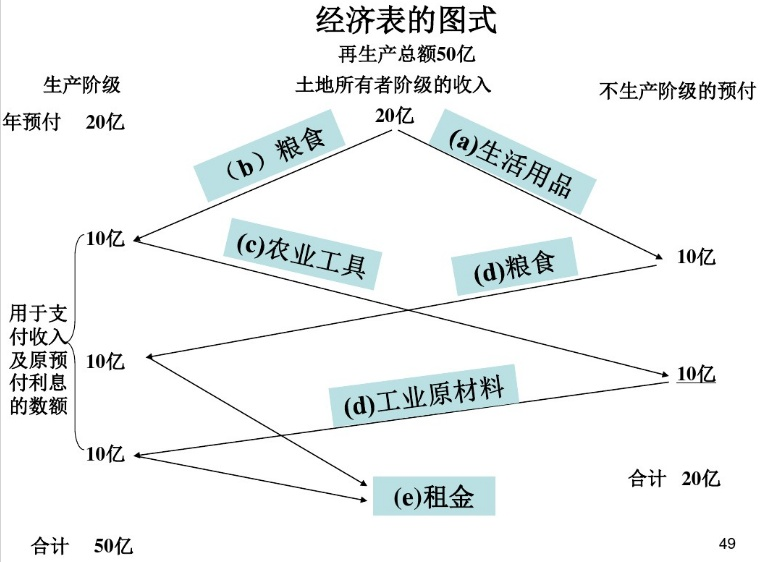
\includegraphics[width=\linewidth]{kuinai.jpg}
  \caption{\label{fig:label}摘自知乎 寒霜雪蝶 的文章 }
\end{figure}

重农主义者不仅就经济体不同部门之间的关系建立结论,而且试图量化它们的规模。在这一
方面,重农主义先于诺贝尔奖获得者瓦西里·里昂惕夫于20世纪30年代所提出的著名的“投
入——产出表”,并且先于以计量经济学家而知名的数量经济学家专业小组所做的工作。经济
表证明了经济体不同部门相互依赖的存在。

\subsection{重农主义经济政策}

重农主义者对微观经济理论的贡献不如他们对宏观经济理论的贡献那么大。他们认为,获得
最大收益的愿望是人类经济活动的根本动机。价格在市场中通过经济活动而得以形成;价格
的形成能够被加以研究,因为它受独立于人类已知的自然法则所支配。他们的价格理论不连
贯,但是他们推导自由竞争导致最优价格;如果每个个体都追求自己的私利,那么社会将从
中受益。此外,他们认为,净产品的唯一源泉是农业,据此推断税收负担将最终依赖于土
地。……重农主义者开始意识到在经济体不同部门活动一体化过程中价格所起的作用。像更
加敏感的重商主义者一样,他们认识到,看上去在市场经济中独立经营的个人,实际上是在
为其他人而经营,这些独立的活动通过价格体制结合在一起。

重农主义者认为,存在一种比人类所设计的任何秩序都优越的自然秩序,所以,他们把经济
体想象成在很大程度上是自我规制的,并因此拒绝重商主义体系所施加的控制。政府特有的
任务是实行自由放任的政策——对事物不加干涉。这一观点被斯密以及后来的经济学家所领悟。

重农主义者认为,经济增长的主要障碍来自重商主义者对国内与国外贸易的规制政策。他们
尤其反对重商主义者的税收体制,提倡对土地征收单一税。

反对法国禁止谷物出口,反对对谷物价格控制。因为重农主义者没有预见到制造业的发展,
所以他们推断自由放任政策将引起法国农业的巨大增长,就像封建经济的小规模农业被大规
模农业所替代一样。因而,法国经济体的财富与权力也将增加。……重商主义者提倡鼓励贸
易顺差的政策——尤其是国际贸易形式的交换。重农主义者则认为净产品的源泉是农业(生
产,而不是交换),并主张自由放任会引起农业生产的增加,最终引致更大的经济增长。

\section{西班牙经济思想}

哥伦布1492年发现新大陆,西班牙成为强国,黄金大量流入造成西班牙国内价格水平上
升……货币数量论……

马丁·阿斯皮利奎塔的成就在于他能够观察到西班牙价格总水平的上升,并从通货膨胀很多
可能的原因中抽象出金银流入与价格上涨之间的关系。货币数量论的脉络:阿斯皮利奎塔——
马歇尔——福利德曼。

像其他经院哲学著作一样,路易斯·摩里纳关于公正与法律的著作本身就在关注发展中的经
济体的道德方面。他主张,在能够对任何一个特定市场作出道德判断之前,有必要了解特定
的市场事实上是如何实行的。……他经济陈述的16世纪的观点,即我们今天所称的供需定理
以及货币数量理论。

像英国与法国后期重商主义一样,在西班牙重商主义末期,经济学家们很少倾向于支持政府
在对外贸易上的严格规制,而是更多倾向于自由的经济思想。彼得罗·罗德瑞库兹·康姆庞曼
斯伯爵是一位相当多产的经济学家。他认为美洲流入到西班牙的金银具有可怕后果。因为西
班牙人能够比较便宜买到法国与英国的产品,所以,西班牙的生产能力就不能像欧洲其他国
家那样得到充分发展,这将最终导致金银从西班牙流向英法及低地国家。康姆庞曼斯提倡给
予外贸较大自由以及其他一些措施,这使得他既是一位重要的后期重商主义者,也是一位早
期的自由主义者。

\section{总结}

重商主义者和重农主义者公认经济体能够被正式加以研究。同时,他们发展抽象方法,也是
第一批模型构建者。……所以有充足的理由将重商主义者与重农主义者视为第一批经济理论
家。

威廉·配第在本质上是一个重商主义者,其重要性在于他最早试图将经济学置于经验观察之
中。斯密对政治算术的反对,以及获取相当精确数据的难题,使量化运动延迟了将近一百年。

就重商主义的死亡来说,可能没有比大卫·休谟的宣言总结得更好的了:“我由此要斗胆声
明,不仅作为一个人,而且作为一个英国人,我祈祷德国、西班牙、意大利甚至是法国自身
的商业繁荣昌盛。”

\part{古典经济思想及其批判}

通常所说的经济学古典时期,涵盖了一百多年的经济思想,其方向与主要贡献者几乎为英国
人所垄断。

从1776年到1820年几乎是斯密时代,从大约1820年到19世纪50年代是李嘉图时代,从19世纪
50年代到19世纪90年代是约翰·斯图亚特·穆勒时代。

另外两位先行思想家是马尔萨斯与马克思,尽管他们在某些方面来看属于古典学派,但是与
作为古典经济学的拥护者相比,他们作为古典经济学批评家的意义更大。马尔萨斯的人口理
论符合古典理论,但是马尔萨斯在他对经济体某些宏观方面的分析中,以及在他对地主阶层
的作用与重要性的捍卫中,却引人注目地背离了正统的古典传统。但是,我们将单独考察马
尔萨斯与李嘉图之间关于经济体自动实现资源充分利用的著名论战。卡尔·马克思从古典经
济学中汲取了一些因素,加入了不同的看法和一些新的分析概念,得出了与古典理论及政策
直接相对立的结论。

\subsection*{古典政治经济学}
\addcontentsline{toc}{subsection}{古典政治经济学}

与重商主义思想最大的不同是,他们对经济力量自然运作所产生的结果持赞同态度。在古典
经济学家眼里,经济体制通常是和谐的,这与重商主义者与经院哲学的信仰尖锐对立,重商
主义者与经院哲学均认为市场的特征在于不和谐,需要进行限制和干预。

法国重农主义者最早引人注目地提出了下面的观点,即针对相对稀缺性产生的冲突,市场自
动地提供和谐的解决办法……政府应当对经济体采用自由放任的政策……

古典学派确信借助自由这一手段,经济体能够最有效率地运行。他们断言,个人与厂商应当
不受政府干预地自由交易。除此之外,古典学派认识到,政治自由与经济自由是不可分割地
绑在一起的,亮着彼此影响。

但他们也非常了解社会冲突,尤其是地主与那些提倡经济增长与变革,并从中获益的人之间
的冲突。正像斯密与李嘉图两人所理解的那样,资本主义的长期趋势导致了这些不和谐的后
果。

经济体制中和谐概念相关的两条显著的发展路径。一方面是,主流正统经济思想尽管一直不
断地接受和谐运行的经济体制这一基本前提,却正通过越来越多地鼓吹经济问题的政治反应
而非经济反应,缓慢而稳定地弱化这一前提。另一方面,一些非主流经济学家否认古典经济
学所认同的和谐性,并发现了体制中的一些基本冲突,这些冲突需要对制度结构进行主要变
革才能加以解决。马克思主义思想是下面这种经济思想最重要的例子,即认为经济体制充满
了矛盾冲突,通过市场力量无法予以解决。

古典经济学派的第二个特征是它对经济增长的关注。……宏观……所以古典经济学家致力于
发掘决定经济增长率的力量、文化、政治、社会、历史因素。这方面凯恩斯主义者的主要关
注点是决定经济活动水平的力量。他们考虑某一时点上一个经济体是否在低于资源充分利用
的水平上运用。古典经济学派对这一问题并不感兴趣,因为他们已经假设经济体倾向于在资
源充分利用的水平上运行。当现代宏观经济学背离凯恩斯主义宏观经济学时,又回到了这些
相同的问题与假设上来,所以,现代宏观经济学家有时也被称为“新古典经济学家”。

古典经济学家对增长的关注使得他们去研究市场,研究作为资源配置者的价格体制。……古
典学派延续了重商主义者的传统,因为两者都聚焦于我们今天所谓的“宏观经济学”。

相比古典经济学,新古典经济学在比较静态的框架中研究市场,目的是使下面的这些问题更
加清楚,即什么力量决定了相对价格,生产了什么种类与数量的消费者产品,利用了什么种
类与规模的经济计划,收入的个人分配与功能分配是如何决定的。直到19世纪70年代,初生
的新古典经济理论才将经济学家的注意力从增长上引开,几乎专门研究有关在供选择的用途
之间分配稀缺资源的微观经济问题。

斯密经济学的最后一个统一特征代表了与重商主义思想的显著背离。尽管重商主义者的理论
结构是不牢固的,但是他们相信自己有能力了解经济体的运行。一旦他们认为自己获得了这
方面的知识,就会认为对他们所洞察的经济体运行中的任何缺陷进行修补是合适的。这种修
补要么通过变更制度结构,要么通过允许政府干预来实现。……重商主义者的角色认知与亚
当·斯密的怀疑论完全相对,斯密向胆敢以其判断来替代市场判断的政治家贤人提出了质疑。

\subsection*{马克思的政治经济学}
\addcontentsline{toc}{subsection}{马克思的政治经济学}

卡尔·马克思是古典经济学最重要的批评家,也是打造古典(classical)一词的人。马克思
是经济思想史的学生……影响马克思的最重要的经济学家是李嘉图。尽管古典经济学派发现
经济体是基本和谐的,并因此提倡自由放任的政府政策,但他们同时也发现了很多冲突。其
中之一就是地主与资本家之间的冲突。马克思指向资本家与劳动者之间的经济冲突。他改造
了古典学派的劳动价值理论以支持他的观点,即劳动者受到资本家的剥削。

古典经济理论与新古典理论不同,其分析的事物与结构是动态的。亚当·斯密集中研究经济
增长,大卫·李嘉图对资本主义中发生的收入分配的长期变化感兴趣。马克思的经济分析只
是其兴趣点的一部分,他的兴趣点是引起历史变革的力量。然而,古典学派所研究的一些相
同的动态问题,也引起了马克思的兴趣,例如,随着时间的变化,收入分配发生怎样的变化,
利润率将采取怎样的进程,大众福利水平的前景如何。

李嘉图和马克思都对劳动价值论感兴趣,但并不是因为它解释了某一时点上什么力量决定了
相对价格,也不是因为它把在可替代的用途之间有效分配稀缺资源的问题说得更清楚。马克
思想表明,剥削是如何根植于劳动者不拥有生产手段的体制中的;李嘉图则运用劳动价值论
来解释随着时间的变化收入分配的变化。

马克思对古典经济学的另一借鉴:对古典学派来说,主要的参与者是资本家、地主、劳动者。
在某种意义上,古典理论是对经济运行和对这些阶级的未来的一种分析。古典学派与马克思
都将社会中的动态因素视为资本家阶级活动的结果。

古典学派与马克思之间的差异比他们的相似之处更加显著,他们之间最重要的分歧是相互抵
触的意识形态上的观点。古典学派发现,资本家的利润动机导致经济体中资本的有效配置,
并导致储蓄,这将促进经济的增长和财富的增加。马克思则将资本家的活动看做是最终有害
于无产阶级和社会的。

\chapter{亚当·斯密}

\section{亚当·斯密的博学多才}

经济学家、大学教师。私密讲授一系列课程,其中包括我们现在所称的社会科学与人类学,他
主要对道德哲学感兴趣。他注意到经济自由与政治自由之间的重要关系,私人财产权利与公
正状态之间的重要关系,以及由利己主义所推动的个体与由关注其行为对他人产生的后果所
推动的个体之间的重要关系。

曼德维尔的讽刺风格令其对重商主义立场的表述广为流行。曼德维尔与斯密都是从人类利己
本性这一相同的假设出发,但却得出了相反的结论。曼德维尔主张,个人对私利的追求,会
产生很多不良的社会和经济后果,因此他为政府干预经济构建了一个实例。

斯密所处的时代,已有的不同研究领域之间不存在清晰的界定:哲学、自然科学、社会科学、
道德都被当做真理统一体的不同方面来对待,而不是当做单独的学科。此外,从事研究的知
识精英受到了严格意义上的教育,他们被要求掌握最宽广的人类知识。

这种多学科方法的一个后果是,那些像亚当·斯密一样,主要探求我们现在称为社会科学与
道德知识的人认为,牛顿在物理学中所建立的科学严密性,在他们主要努力的领域中也能够
达到。显然,斯密及其同时代的人,能容易地把今天被称做实证性的问题与规范性的问题相
混合。

斯密对经济学范围的认识,继承了英国重商主义者的观点。他对解释国民财富的性质与原因
感兴趣。现代经济学家将斯密描述为对决定经济增长力量感兴趣的宏观理论家。然而,斯密
所考察的力量比现代经济学家所研究的力量要宽泛,他用政治的、社会的、历史的材料来填
充其经济模型。他注意到了相对价格的决定——今天包含在微观经济理论中——但是,它的主要
兴趣在经济发展与推动经济增长的政策上。

因为斯密断定经济体总是充分使用其生产资源的,所以,他没有触及宏观经济学中的一个重
要问题:当经济体的生产能力既定时,什么力量决定收入与就业水平?

斯密将演绎理论与历史描述相结合的方法论也值得注意。他的理论模型缺少优雅与严密,但
是,他对经济体中的相互关系和经济体运转的描述,以及他将历史实例组合进分析中的能力,
是无可比拟的。

\subsection{新教与资本主义:是否是一种因果联系}

R.H·托尼《宗教与资本主义的兴起》,马克思·韦伯《新教伦理与资本主义精神》认为宗教
改革与新教伦理观的兴起,极大地促进了产业革命与资本主义的出现。我们已经了解,天主
教教义的根源在亚里士多德,它与新产业秩序的成长相敌对。但是,约翰·加尔文及其追随
者的教义,确实与经济活动兼容的。韦伯--托尼的论题是宗教直接有助于资本主义体系的兴
起。韦伯与托尼受到很多经济学家的批评,然而,他们两人都是细致小心的学者。他们承认,
在宗教观点、经济行为以及经济制度之间确定因果关系的次序是极为困难的。例如,他们认
识到,因果关系也会涵盖在从经济制度到宗教观点中,产业革命与资本主义的发展可能同等
程度地说明了新教伦理观的发展与认同。

经院哲学教条主张,表现为个人财富的经济活动的成功,是罪孽行为的强烈指征——索要过高
的价格,以高利率放款,过分注重收益却少关注灵魂救赎。根据经院哲学伦理观,经济活动
的成功显示了永恒拯救的语言。经院哲学还认为,努力工作有益于灵魂,炫耀性消费应当予
以避免。强调劳动与节俭美德的宗教观点,被认为是促进现代经济社会出现的主要因素。

\section{斯密的市场分析与政策结论}

有两种可行的方法来分析亚当·斯密的著作。一种方法是考察整体的理论结构与政策含义,
这些政策含义或者内在于理论体系中,或者由斯密明确地予以表述。另一种是详细地考察理
论结构,来评价理论内在的一致性抑或一致性的缺失(专注于理论技巧方面)。本书专注于
第一种方法,全面地考察斯密的理论结构,同时考察从更详细的经济分析中产生的政策结论。

斯密作为一位经济学家的强大实力在于,他洞察了:(1)经济体组成部分的相互依赖;(2)
用来推动一国财富的政策。

\subsection{前后关联的经济政策}

斯密提倡自由放任,并不是因为他认为市场是完美的,而是因为联系到他所处时代英国的历
史与制度结构,市场通常会比政府干预产生更好的结果。

斯密是经济学艺术大师。前后关联的经济政策(contextual economic policy),就是另一
种表达经济学艺术观点的方式。后来的经济思想家在方法上有所改变。李嘉图对自由放任的
倡导是前后不关联的,这与其抽象的无历史记载的方式相一致。穆勒与马歇尔回归到斯密的
传统上来,在所做的分析与政策结论中,他们明智地设法将理论、历史与当时的制度相结合。

现代经济学正在偏离抽象的理论化,很多现代经济学家与政治学家正在考察政府与政府政策
如何才能实际发挥作用。这些现代公共选择理论家们劳动的一个无意识结果,可能就是重新
引起人们对前后关联的经济政策——经济艺术的兴趣。

\subsection{自然秩序、和谐与自由放任}

受到物理学发展的影响,重商主义者和斯密认为,依靠严格的分析是有可能发现经济体的规
则的,他们都就人类本性作出相同的假定:人类是有理性的,是有私心的,很大程度上受经
济利己主义的驱使。

斯密体系与大多数重商主义者体系的一个区别在于他的假设,即竞争性市场在极大程度上是
存在的,在这些市场内部,生产要素自由流动,从而提升了它们的经济优势。第二个区别是
下面的假设,即经济体的自然运转过程,能够比人类做出的任何安排更有效地解决冲突。

\begin{quotation}
  他受着一只看不见的手的引导,去尽力达到一个并非他本意(人的自利)想要达到的目的。
  并非其本意对社会来说不一定是坏事。他追求自己的利益,往往能使他比在真正出于本意
  的情况下更有效地促进社会的利益。我从未听说那些假装为公共利益而从事贸易的人会做
  什么善事。的确,这种虚伪在商人中间并不常见,所以,基本不需要费什么口舌来劝阻商
  人的这种虚伪。
\end{quotation}

斯密得出其主要政策结论的推论法非常简单。人类是理性的,是有私心的,受利己主义的驱
使。如果放任不管,每个个体将追求他或她自身的私利,在促进私利的同时也促进了社会利
益。政府不应当干预这一进程,而应当遵循自由放任的政策……资本家是根据最终产品来看
待市场的,为了增加收入而生产人们所期望的商品。资本家之间的竞争,将使这些产品在某
一生产成本下生产出来,这一生产成本将返还生产者正好足够支付不同生产要素机会成本的
一个数量……消费者通过他们在市场上的货币选票来引导经济体;消费者欲望的改变在价格
的上升和下降——因而在利润的上升和下降中得到体现。斯密断定,在没有计划和政府指导的
情况下,市场如何导致消费着欲望在最低可能的社会成本上得到满足,这将是一个其妙的过
程。按照现代经济学的术语,斯密断定,在没有政府干预的竞争性市场上会出现资源的最佳
配置。

\subsection{竞争性市场的运作}

斯密能够比以前的经济学家更准确地详细说明,源于竞争的价格在长期中为什么等于生产成
本这一道理。在他对价格形成与资源配置的分析中,他将短期价格称为“市场价格”,将长
期价格称作“自然价格”。他主要关注长期自然价格的形成。……因而产生的自然价格将使
资源得到最佳配置,原因在于消费者以最低的可能成本获得了他们想要的产品,同时,最大
的增长率得以保证。

确立了竞争性市场的优越性之后,斯密便毫无困难地构建起他反对垄断与政府干预的论
据。……他意识到垄断者将会通过限制产量来索要较高价格。值得注意的是,斯密提倡的自
由放任是以竞争性市场的存在为假定性条件和准则的。

私密反对政府干预经济的主张具有政治的、哲学的、经济的基础。他认为,一般而言,任何
政府干预都是不合意的,原因在于它侵害了个人正常的权利和自由。……斯密认为,尽管重
商主义者关于政府干预的很多主张都声称促进了社会利益,但其实是增进了个人私利。对国
内与国外商业的管制,不是有利于国家,而是有利于商人。……鉴于政府的运作方式,它们
将不可避免地有害于而不是有益于社会利益。从这个意义上讲,现代公共选择理论的根源,
可以追溯到亚当·斯密关于商人如何利用政府使自己富足的认识上。

然而,斯密对自由放任的拥护是有所限定的,因为他引用了几个领域,并认为在他所处时代
历史的、政治的、制度的背景下,在这些领域实行政府干预是必要的。例如,保护幼稚产业
的关税;政府应当提供国家防卫,修建并维护道路和学校,维护公正以及进行人口登记。更
重要的是,斯密提倡政府提供具有极大社会有益但私人市场因为没有充足利润而不去提供的
产品,以此来限定他对自由放任的主张。例如,教育。如果听任市场调节,那么市场所提供
的教育将少于社会所需要的(现代福利经济学的大量内容涉及外部性、第三方或溢出效应,
以及如果获得最大社会福利该如何考虑这些问题)。

在倡导自由放任政策的过程中,斯密非常谨慎。只有当竞争性力量存在并将私利引向社会利
益时,看不见的手才用来结合公共利益与私人利益。

\subsection{资本与资本家}

他指出,一国的现有财富取决于资本积累,原因在于资本积累决定了劳动分工和参加生产性
劳动的人口比例。其次,斯密断定资本积累也会导致经济发展。再次,与资本积累相结合的
个人私利导致资本在各产业之间的最佳配置。

资本家在经济体运行中扮演着主要角色。他对财富与利润的追逐,引导着经济体实现资源的
有效配置与经济增长。在一个私有财产经济体中,资本的来源是个人储蓄。斯密认为,劳动
并不能够积累资本,原因在于工资水平仅仅能够满足直接的消费欲望。他观察到,部分地主
阶级拥有足够的收入来积累资本,但是,他们却将这些收入花在非生产性劳动上,以满足他
们奢侈生活的无限欲望。……一部分正在兴起的产业阶级是对社会有益的人,他们为了利润
而奋斗,努力积累资本,通过储蓄和投资来增加他们的财富。因此,有利于资本家的收入不
平等分配,具有巨大的社会重要性。没有收入的不平等分配,就不可能有经济增长,因为全
部的年产出将被消费掉。

\subsection{斯密对政策的影响}

它的主要政策结论是政府应当接受自由放任的政策。这一结论对工业化国家的经济政策影响
巨大。它已经成为社会的经济意识形态……可以说,没有哪一个观点,没有哪一个经济学家,
对经济与社会的发展产生过更重要的影响。

\section{国民财富的性质与原因}

在《国富论》第一句中,斯密解释了国民财富的性质这一概念。这样他就将自己的观点与重商
主义者和重农主义者的观点区别开来。

\begin{quotation}
对每一个国家来说,供应全国人民每年消费的生活必需品与便利品的根本来源,是全体国民
每年的劳动;那些被消费掉的必需品与便利品,如果不是由该劳动直接生产出来的,便是用
该劳动的产出物向国外购买的。
\end{quotation}

在《国富论》全书的很多地方,斯密严厉指责重商主义者关注金银的积累,以及将金银等同
于一国的财富。……财富是产品与服务的年流量,而不是贵金属的累积储备量。他也揭示了
出口和进口之间的联系,认识到出口的基本作用是支付进口。此外,在他的开篇语中,他暗
示说经济活动的最终目的是消费,在《国富论》后面的章节中,他就这一立场予以了给全面
的阐释。这就进一步将斯密的经济学与重商主义的经济学加以区分,后者将生产视为其本身
的目的。最后,在强调劳动是一个国家财富的源泉时,斯密又与重农主义者不同,后者强调
的是土地。

\begin{quotation}
  消费是所有生产的唯一目的与意义;生产者的利益应该受照顾,但不该超过也许是促进消
  费者利益所必要的程度。……但在重商主义里,为了生产者的利益,消费者的利益几乎不
  断的被牺牲;它似乎认为,所有勤劳与商业活动的最终目的与意义,在于生产,而不在于
  消费。(《国富论》第四卷第八章末尾)
\end{quotation}

斯密继而建议,国家的财富应当按照人均指标来衡量。其实,斯密的这一看法一直被继承到
现在。

\begin{quotation}
消费是所有生产的唯一目的与意义;生产者的利益是应该受照顾,但不该超过也许是促进消
费者利益所必要的程度。此一箴言是如此纯然不证自明,只有想法荒谬的人,才会想要加以
证明。但在重商主义里,为了生产者的利益,消费者的利益几乎不断的被牺牲;他似乎认为,
所有勤劳与商业活动的最终目的与意义,在于生产,而不在于消费。

就限制所有可能和我们自己的产物或制造品一起竞争的国外商品进口而言,国内消费者的利
益显然是生产者利益的牺牲品。完全是为了后者的利益,前者才被迫承受这种独占几乎总是
会带来的价格上升的压迫。(谢宗华、李华夏所译《国富论》527页)
\end{quotation}

\subsection{国民财富的原因}

斯密主张,一个国家的财富即我们今天所称的一个国家的收入,取决于:(1)劳动生产力;
(2)有效使用或者生产性使用的劳动者的比例。因为他假设经济体将自动实现资源的充分
利用,所以他只考察那些决定一国产品与服务生产能力的因素。

\begin{description}
\item [劳动生产力] 在《国富论》第一篇中,斯密阐述了劳动生产力取决于劳动分工,强
  调这一原理。尽管斯密认可专业化与劳动分工的经济利益,但他也察觉到一些严重的社会
  成本。劳动分工的一个社会缺点是工人被赋予重复性的任务,这些任务很快就变得单调乏
  味。人们成了依赖于生产过程的机器……而失掉人性。但是,斯密毫不怀疑最终通过劳动
  分工增加了人类福利。

  劳动分工依次取决于斯密所谓的市场范围(extent of the market)与资本的积累。市场
  越大,可销售的数量越多,劳动分工的机会就越多。……劳动分工受到资本积累的限制,
  原因在于生产过程是耗时的:随着劳动分工的增加,劳动者不在为其自身的消费生产产品,
  在耗时的生产过程中,必须保持一定的消费品储备来维持劳动者。这一数量的产品来自于
  储蓄,即斯密所谓的资本。资本家的一个主要功能是为缩短生产开始与最终产品销售之间
  的时间间隔而提供手段。


\item[生产性与非生产性劳动] 根据斯密的观点,资本积累也决定了生产性劳动者与非生产
  性劳动者之间的比率。斯密对是否生产性劳动的尝试另其困惑,也反映了他所做出的规范
  或价值判断。然而,它也表明斯密意识到经济增长的问题。他主张生产可销售商品所使用
  的劳动是生产性劳动,而生产服务所使用的劳动则是非生产性劳动。资本家有益于经济增
  长与发展;而地主在仆人和其他无形产品上的花费、司法与军事人员等则是浪费。“资本
  因过度借鉴而增加,因挥霍浪费和不正当行为而减少。”

  斯密强调,通过下列分配方式,可以获得最高的经济增长率,即将大量收入分配给储蓄和
  投资的资本家,而将少量收入分配给地主,因为他们将钱花在仆人身上,并且“没有留下
  任何东西作为消费的回报。”此外,因为经济增长受到政府非生产性劳动支出的约束,所
  以较小政府就可以给政府征收较低的税,以便他们能够积累更多的资本。
\end{description}

\subsection{对国民财富原因的总结}

\begin{figure}[ht]
  \centering
  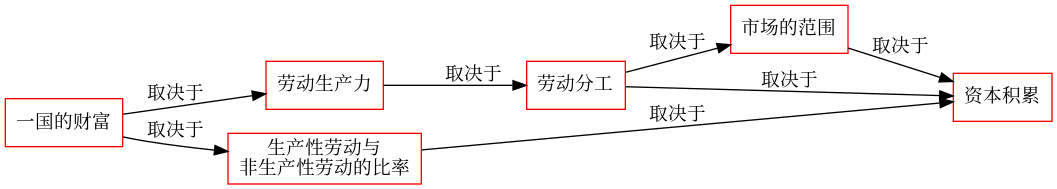
\includegraphics[width=\linewidth]{simi.png}
  \caption{\label{fig:simi}一国财富的决定因素 }
\end{figure}

增加劳动力,通过机器工具或者劳动分工等提高已雇佣的劳动者的生产力,几乎都需要追加
资本。

对亚当·斯密来说,资本积累毫无疑问要求一个自由市场与私人制度框架。……在私人财产
体制中,对高资本积累率的进一步要求就是不平等的收入分配。

\section{国际贸易}

斯密主张非规制的对外贸易,理由是如果两国各自用生产成本较低的产品去交换生产成本较
高的产品,这种交换对双方来说都是有利的。用经济学的语言来说,这就是著名的对外贸易
的绝对成本学说。而且,这一学说不局限于国际贸易,它也适用于一个国家的内部贸易。

用现代经济学语言来说,随着劳动变得越来越专业化,存在收益递增(成本递减)的情形。
斯密认识到,如果两个个体出生时拥有相等的天赋并保持这一天赋不变,如果他们实行分工
并交换其产品,那么,他们中的任何一个人都不具有优势。然而,如果两个个体通过劳动专
业化变得更加熟练,那么两人所生产产品的成本都减少了,两人都从专业化与贸易中获益。
从斯密的这一见解中,产生了如下对自由贸易的发展至为关键的共识,随着时间的变化,任
何国家都能够通过专业化与劳动分工自动得获得生产某些产品的绝对成本优势,并且所有国
家都能够从此产生的国际贸易中获益。斯密认为,自由放任的政策将不断导致所有国家更高
的福利水平。

斯密在其广泛的社会科学与历史框架中,就经济分析做出的较少抽象而更多制度性的见解,
以及所使用的方法,直到今天还吸引着越来越多的注意力。政治经济学这一术语从经济学行
话中已经消失一百年了,但是,很多经济学家现在正迫切要求回归到更加斯密化的经济学范
围中,就像属于所暗示的那样。公共选择理论与新制度经济学两者的根源都能追溯到亚当·
斯密。

\section{价值理论}

价格或价格

(1)是什么决定了一件产品的价格?用现代经济学的语言来说,是什么决定了相对价格?(2)
是什么决定了价格总水平?(3)什么是福利的最佳度量标准?第一和第三个问题是现代微观
经济学的部分内容;尽管第二个问题难以用通常简单的“宏观--微观二分法”来判断,但是
一般情况下它都被包含在宏观经济学的宽广范围中。对上述任何一个问题,斯密都没有提供
明确的答案。原因在于,他自己对什么决定了相对价格的讨论,与自己试图发现不同时期福
利变化的度量相混合。
一组经济学家认为,斯密有三个相对价格理论(劳动成本、劳动支配、生产成本),以及一
个解释价格总水平的理论。另一组经济学家则认为,斯密研究了生产成本的相对价格理论,
度量不同时期福利变化的理论,以及价格总水平理论。后一组经济学家否认斯密曾涉及劳动
的相对价格理论。我们认为,斯密对这些理论都进行了试验:对于简单社会而言的由劳动成
本与劳动支配所组成的相对价格理论;对于发达经济体而言的生产成本的相对价格理论;衡
量不同时期福利变化的指数形成过程;以及解释价格总水平的理论。

\subsection{相对价格}

尽管亚当·斯密将相对价格解释为由供给或者生产成本单独决定的。但是,他并没有完全忽
视需求的作用。他认为市场价格或者短期价格是由供需双方决定的。自然价格,或者长期均
衡价格通常取决于生产成本,虽然有时斯密也表示自然价格取决于需求与供给。这些不一致
为经济理论史家们争论斯密的真正含义提供了丰富的机会。

斯密对他所处时代经济体中相对价格形成的分析,区分为两个时间段和经济体的两个宽泛的
部门,分别是短期与长期、农业与制造业。在短期或者市场阶段,斯密在制造业与农业中都
发现了向下倾斜的需求曲线与向上倾斜的供给曲线;因此,市场价格取决于需求与供给(两
个曲线的横坐标均为数量,纵坐标为价格)。斯密对长期中发生的更为复杂的“自然价
格”的分析,包含着一些矛盾。对农业部门来说,自然价格取决于供需,原因在于长期供给
曲线向上倾斜,表明成本递增。但是,对制造业部门来说,长期供给曲线有时被假定为完全
富有弹性(水平的),表明成本不变,价格完全取决于生产成本;在分析的另一些地方,又
向下倾斜,表明成本递减,自然价格就取决于供需双方。

斯密对制造业产品自然价格决定因素的陈述,存多种解释。……斯密前后一贯地注意到需求
在自然价格形成中,以及将资源在经济体不同部门之间配置时的作用。不过,无视长期供给
曲线在制造业中的形状,主要强调生产成本对自然价格的决定,这是斯密以及后来的古典经
济学家的特点。

经院哲学对相对价格问题感兴趣,原因在于他们关注交换的道德方面;重商主义者则是因为
他们认为财富是在交换过程中产生的。尽管斯密有时也从道德方面讨论相对价格,然而他对
相对价格的决定因素感兴趣还有更重要的原因。一旦经济体实行专业化与劳动分工,交换就
成为必须。第一,如果交换处于高于物物交换水平的状况下,就会存在交换媒介——货币——的
问题。第二,存在价值或相对价格的问题。用斯密的话来说就是,什么原理决定了产品的相
对价值或交换价值?第三,存在经济体的产量如何在那些参与生产的主体之间进行分割(收
入分配)的问题。

\subsection{价值的含义}

\begin{quotation}
必须注意“价值”一词有两个不同的意思。有时它表示某一特别物品的效用;有时则表示该
物品给予占有者购买其他物品的能力。前者也许可称之为“使用价值”,而后者或许可称之
为“交换价值”。那些具有最大使用价值的物品,往往几乎或完全没有交换价值;相反地,
那些具有最大交换价值的物品,却往往几乎或完全没有使用价值。没有什么东西比水更有用,
可是水却几乎买不到任何东西。相反的,钻石几乎没有使用价值;但拿钻石去交换,往往可
以得到大量的其他物品。(谢宗华《国富论》21页)
\end{quotation}

按照斯密的观点,交换价值是一种商品购买其它产品的能力——它的价格。这是市场所表达的
一种客观度量。他关于使用价值的概念是含糊的。一方面是,使用价值有道德内涵,因此是
对经院哲学的回归。比如钻石基本没有什么使用价值。另一方面,使用价值是一种商品满足
需要的能力,是因持有或消费一件产品而获得的效用——总效用、平均效用、边际效用等。斯
密的关注点是总效用,这就模糊了他对需求如何在价格决定中发挥作用的理解。(直到斯密
创作《国富论》一百年之后,边际效用与价值之间的关系才被经济学家所理解。)显然,水
的总效用超过了钻石的总效用。然而,因为商品的边际效用经常随着其消费得更多而递减,
钻石的边际效用就更高。我们愿意为一件商品所支付的价格——我们对获得又一单位商品所寄
予的价值——不仅取决于商品的总效用,而且取决于其边际效用。因为斯密对总效用的关注,
斯密就既不能为“钻石——水悖论”找到满意的解决办法,也不能了解使用价值和交换价值之
间的关系。

\subsection{斯密关于相对价格}

因为斯密对相对价格的决定因素有些困惑,所以,他发展了与这些因素相关的三个独立的理
论:(1)劳动成本价值理论;(2)劳动支配价值理论;(3)生产成本价值理论。

他假设了经济体两种截然不同的状态:初期野蛮状态或原始社会,其中资本还没有被积累起
来,土地未被使用;发达经济体,其中资本与土地不再是资源充足的产品(他们具有超过零
以上的价格)。

\begin{description}
\item[原始社会中的劳动成本理论]

按照斯密的劳动成本理论,在还不存在土地与资本的经济体中,或者土地与资本还是无限充
足的自然资源的经济体中,一件产品的交换价值或者价格,由生产产品所需的劳动量决定。
斯密认识到生产一件产品所需的劳动量不能简单地用时钟表示的时间数量来度量,原因在于,
除了时间之外,也必须考虑有关的精巧或者技能,以及任务的艰难与困苦。

在这一点上,斯密遇到了所有的劳动成本价值理论都遇到的,仍未被后来的经济学家成功地
予以解决的一个难题。如果劳动量是一个以上变量的函数,那么,我们必须找到一种方法来
说明所有变量的相对重要性。斯密试图将时间、艰难程度以及精巧程度还原为一个共同分母
的问题。

但斯密的建议仅仅是重申了问题,而不是为问题提供解决办法。其价值理论的目的是解释相
对价格的那些决定力量,但是工资本身就是其理论必须解释的经济体中的很多价格之一。斯
密利用一套价格,也就是工资,来解释另一套价格。

\item[原始社会中的劳动支配]
按照斯密的观点,在劳动支配理论中,一件产品的价值等价于产品的劳动成本。1海狸=2野
鹿。

\item[发达经济体中的劳动理论]
  资本已经被积累,土地也已被利用,它们不再是资源充足的产品。并且,一件产品的最终
  价格,也必须包括当做利润的资本家的收益以及当做地租的地主的收益。最终价格形成了
  由工资、利润、地租这些要素报酬所构成的收入。


\item[相对价格的生产成本理论]
  斯密一直努力发展经济体中产品最终价格不仅仅包含劳动成本的劳动价值理论,但是他最
  终还是放弃了下面的这种观点,即任何劳动价值理论都适用于像他所处时代一样发达的经
  济体。斯密似乎发现,一旦资本被积累起来,土地被加以利用,并且,一旦必须支付利润、
  地租、还有劳动,能唯一适当地解释价格的就是生产成本理论。在成本理论中,一件商品
  的价值取决于对所有生产要素的支付:除了劳动之外,还有土地和资本。在斯密的体系中,
  利润这一术语既包含我们今天所理解的利润,也包括利息。在斯密假设平均成本不随着产
  量增加而增加的地方,无论使用总成本还是平均成本,这一计算都能得出相同的价格。在
  斯密假设平均成本随着产量而变化的时候,价格就取决于供需双方。然而,在分析长期自
  然价格的决定时,即使当供给曲线不被假设为完全富有弹性时,斯密也强调供给与生产成
  本。斯密主张,竞争占优势的地方,商人、劳动者、地主的私利将导致与生产成本相等的
  自然价格。
\end{description}

\section{分配理论}

劳动是为大部分家庭所拥有的唯一的生产要素,因此,家庭的收入一般取决于工资率与工作
时间的长度。拥有资本的那些家庭所获得的财产收入量,取决于家庭所拥有的资本与土地的
数量以及这些要素的价格。

因为工资、利润、底足都是经济体中的价格,所以,它们的相对价格——连同个人出售的劳动、
资本、土地数量一起——决定了收入的分配。尽管收入分配不是斯密主要关注的内容,他还是
提出了几个不同的有时甚至矛盾的工资、利润、地租理论。我们将只限于涉及其分析中领先
于后来经济学家的一些方面进行阐述和批判。

\subsection{工资}

在《国富论》第一篇第八章中,他提出了最低工资理论、生产力理论、讨价还价理论、剩余
要求权理论、工资基金理论……有矛盾之处。

斯密指出,在对工资的讨价还价过程中,劳动处于劣势。他说,因为雇主比雇员的人数少,
所以雇主能够很容易地联合起来巩固他们的地位。此外,法律允许雇主联合,但是禁止雇员
组成联盟。按照斯密的说法,议会有很多反对提高工资的法案,但没有一个反对降低工资的。
最后,即使在罢工期间或停工期间不雇佣劳动,雇主也有足够的资源来维持他们的生活。但
是在另一方面,“没有工作,很多工人生存不了一星期,很少有人能生存一个月,几乎没有
人能生存一年。”在这些章节中,斯密削弱了市场力量的有益运作过程,并似乎已经意识到
其完全竞争性市场的假设收到了限制。

\subsection{工资基金学说}

斯密在对工资的讨论中,提出了他的工资基金学说,这一观点成为古典经产学的一个重要分
析工具。假定存在一个固定的资本基金,专门用以支付工资。因为生产过程是耗时的,所以
从生产过程开始到产品最终销售之间,需要以前生产的产品供劳动者用于衣食住行等。这些
库存产品或资本被称为工资基金,其来源是资本家的储蓄或者消费中断。给定劳动力和工资
基金的规模,工资率就可以确定为:工资率=工资基金/劳动力。

\subsection{利润}

令人奇怪的是,自己对利润性质与源泉的讨论极其简短。一般而言,古典经济学家都没有做
太多的努力来解释这些。显然,斯密毫无疑问地接受了下面的这种合理性,即利润是因资本
家执行了对社会有用的功能而对他的一种支付(参考工资基金等)。按照斯密的观点,劳动
者允许从其产量中进行利润的扣除,原因在于,劳动者并不拥有工作所用的原料和独立的支
持手段。于是,利润在此就由两部分构成:纯利息收入和风险收入。

在斯密的原始经济体中,劳动者获得了全部产品,但是在他自己所处的时代,劳动者不得不
与资本家和地主一起分享产品。斯密从未解释为什么要从劳动的产量中扣除利润和地租……

\subsection{地租}

斯密至少提出了四种地租理论,所有的理论都互相矛盾。地租的起源从不同角度被认为是:
(1)地主的需求;(2)垄断;(3)差异化的优势;(4)大自然的施舍。

\subsection{随着时间变化的利润率}

他对不同时期利润率的变化极其感兴趣。他预测,随着时间的推移,利润率将会下降,原因
有三。(1)劳动市场的竞争。资本积累将引起资本家之间在劳动市场上的竞争,其结果是
工资上升。斯密断言工资上升将致使利润下降。(2)商品市场的竞争。斯密推论,随着产
量增加,生产者之间的竞争加剧,结果是商品价格下降,利润减少。这也暗示了整个经济体
生产过剩的可能性,它与斯密所主张的不可能发生生产过剩的观点相冲突。(3)投资市场
的竞争。显然,斯密认为投资机会是有限的,因此,资本积累的增加将致使利润下降。当他
考察什么历史资料对研究利息率的长期趋势有用时,数据支持了他的理论推论。他的确也注
意到一些殖民地的特征是高工资与高利润并存。


\subsection{福利与价格总水平}

《国富论》第一篇第五章“论商品的真实价格与名义价格或其劳动价格与货币价格”。我们
认为,斯密试图在本章回答几个问题,尽管这些问题相互关联,但是当他们被同时加以考察
时,又会产生混淆。他努力去发现:第一,决定价格总水平的因素;第二,不同时期福利变
化的最佳度量。第二个问题更加困难。我们应当怎样用一种明确的方式来界定福利,使得福
利变化能够被度量出来呢?假设经济体制生产唯一的一种最终产品——野鹿。根据所消费的野
鹿数量,就能界定和度量经济体的福利。对社会来说,较大数量的野鹿消费代表了福利的增
加,较少数量的消费则代表福利的减少或者“不幸福”。当我们引进第二种最终产品海狸时,
问题就变得复杂了。我们能毫不含糊地说两者消费都增加,则福利也增加;两者消费都减少,
则福利也减少。但是,如果海狸的消费增加了,野鹿的消费减少了,又该怎样判断福利呢?
社会中,那些给海狸较高评价的人,他们的福利将会增加;那些给野鹿较高评价的人,他们
的福利将会减少。对于一个生产两种或者更多产品的经济体来说,有可能界定和度量其福利
的变化么?斯密试图回答这个问题。

如果用社会的总消费或者产量来界定福利,那么,对多产品的经济体来说,首先要解决的问
题就是,找到一种加总产品数量或者产品消费的方式。这一问题的一个可能的解决方案是,
将所有商品都转换为共同的度量标准。在今天的经济体中,我们通过加总每件商品的货币价
值来度量产量,已获得我们成为GDP的一个总数。从当年到下一年,如果GDP增加了,我们就
能断定福利增加了吗?

通过这种方法来度量多产品经济体中产量的变化,也呈现出一些困难。原因在于,即标准货
币本身是可变的。价格总水平变化,产量的货币价值也变化。斯密考虑了使用黄金或者记账
单位作为共同的度量标准的可能性,但又断定,因为这些商品的价格也在变化,所以在这一
用途上它们不是令人满意的。于是,他转向了劳动,但却发现劳动的价格也随时间而变化。
最后,它能够找到的用来评定福利变化的唯一不变的度量标准是劳动的负效用\footnote{负
  效用是指某种东西所具有的,不但不能给人们带来某种欲望的满足,反而给人们带来了不
  舒适或痛苦的能力。如垃圾、废气一类物品。负效用一般是在消费者消费商品得到最大满
  足程度之后出现的,因为这时消费者对该种商品消费得到的总效用已经达到了最大值,如
  果再继续增加这种商品的消费量,就必然产生负效用。}。

\begin{quotation}
所以,劳动看来显然是唯一普遍的,也是唯一精确的价值衡量标准。或者说,劳动是唯一可
让我们随时随地据以比较各种商品价值的标准。(顾版《国富论》28页)
\end{quotation}

 考虑到斯密关于能够用劳动负效用来计算福利指标的结论,度量福利变化的问题就容易解
 决了。(将货币收入与名义价格转换为实际收入与实际价格后)如果我们能用较少的劳动
 生产相同的产量,那么,我们将拥有更多的闲暇,经济状况就会更好。

 度量福利的变化远比斯密所设想的要复杂得多,然而我们不能涉及全部问题。斯密没有论
 述如何界定或度量劳动的负效用。这一点看来完全是主观的。直到20世纪,正统经济学家
 才对他的假设之一提出质疑,即较多的产品比较少的产品要好,或者说,没有增加劳动负
 效用而使产量增加,必定总会导致福利增加。在斯密的著作中,组成总产量的各种产品不
 是他关注的问题。产量的增加就是福利的改进。斯密及后来的正统经济学家,不考虑扩大
 的产量所带来的“生活质量”,他们较少注意或者不去注意以污染或其他有害外部性存在
 的成本,这些成本是为不断增大的产量所进行的预付。

 确定社会的长期增长率,是亚当·斯密主要关心的一个问题。随着我们步入21世纪,经济增
 长及其原因和结果这一问题又变得突出了。“新增长理论”,罗伯特·巴罗和阿尔伯特·F·
 阿戴斯与爱德华·L·格拉瑟等人的现代经验方法试图了解国家财富的原因。

 \section{总结}

 斯密对经济思想的贡献与影响是巨大的,大大超过他所处时代的其他任何一位经济学家。
 他领会了支配市场经济的重要观念和力量。然而他未能详细阐述关于相对价格、价格总水
 平及福利变化的单独理论,并对它们进行清楚的区分。(其他内容请看前文,不再摘抄)。

 斯密并不是一个纯粹的理论家。相反,他是一位政治经济学家,他能够用描述性的和历史
 的材料来补充市场经济中不同部门相关性这一极其重要的认识……穆勒追随纯粹的理论家
 李嘉图,马歇尔又追随穆勒;穆勒与马歇尔都试图使经济学回归到亚当·斯密前后关联的分
 析与政策上来。很少有例外的是,马歇尔以来的正统经济学家的分析方法,几乎专门集中
 于纯粹的抽象理论,很少关注历史与制度材料,抛弃了斯密的方法论。然而,抛弃了斯密
 自由放任政策主张的非正统经济学家却一直延续着他的方法论。

 \chapter{李嘉图与马尔萨斯}

 李嘉图是金融世界的人士,马尔萨斯则是精神世界的人物。

 \section{大卫·李嘉图——一个理论家的理论家}

李嘉图是一个由股票经纪人转变而成的经济学家,他对经济理论的许多领域都作出了重要贡
献,包括方法论、价值理论、国际贸易、公共财政、收益递减、地租。

\subsection{斯密《国富论》与李嘉图《原理》之间的时期}

李嘉图《政治经济学及赋税原理》1817年出版之前,亚当·斯密1776年出版的《国富论》一
直支配着英国的思想。这期间的四十年,尽管对经济分析有一些重要贡献,但是未出现过重
要的经济理论。托马斯·罗伯特·马尔萨斯在1798年发表了一篇短文,1803年出版了一部著作,
都是关于人口的;1815年,韦斯特、托伦斯、马尔萨斯及李嘉图分别发表了地租概念和经济
意义的短文。

因为马尔萨斯的人口论题对于理解李嘉图理论的某些部分是基本性的,所以我们将首先考察
它;然后再讨论和评价李嘉图;最后,又将回到马尔萨斯,考察他在,政治经济学原理》
1820中所发展的关注经济体在充分就业下自动运转能力的观点。作为经济思想发展中最生动
的辩论之一,马尔萨斯与李嘉图激烈地辩论过这一问题。

\section{马尔萨斯的人口学说}

马尔萨斯的主要论题是人口增加快于食物供给增加,这一观点并不是由他最早提出的。斯密
与本杰明·富兰克林等人的著作中也能找到这一论题。然而马尔萨斯对人口问题的论述影响
最大。

\subsection{对时代问题进行思考性回应的人口理论}

似乎有三个因素。第一个因素是人口对食物供给造成的压力。1790年后,英国进口食物成为
必需,价格也显著上升。第二个因素是低收入阶级在工厂生产代替家庭生产、英国开始城市
化背景下的日益贫困。第三个因素是发生在罗伯特·马尔萨斯与其父丹尼尔·马尔萨斯之间的
争论。丹尼尔·马尔萨斯所接受的戈徳温和康德桑特的基本观点是:个人的特性并不是通过遗
传而获得的,而是通过他或她生活的环境塑造的。戈徳温尤其为他所赶到的周围世界的艰难、
贫困、不幸以及恶行所困扰。他断言,对此负主要责任的是政府,也因此被一些人称为哲学
无政府主义之父。罗伯特·马尔萨斯尤其试图证明,贫穷与不幸并不是社会制度与政治制度的
结果,这些制度的变革不会消除社会的罪恶。罗伯特·马尔萨斯于1798年匿名出版人口论,书
籍全名为“影响社会将来改善的人口原理论说,并评戈德温等学者的学说”

\subsection{人口论题}

马尔萨斯在其短文第一版中所确立的基本原理,建立在两个假设之上:(1)食物对于人类
的生存是必须的,(2)两性之间的性爱是必须的并将保持不变。他推断,与食物供给相比,
人口趋向于以更快的速度增长,这就是贫穷与不幸的原因。尽管马尔萨斯承认土地供给的有
限性,但是他没有利用农业中的收益递减原理来证明经济体不能显著地增加食物供给这一主
张是正确的。……马尔萨斯不认可技术的发展有可能解决人口问题,这也使他的很多理论无
效。

他断定人口控制将会逐步使人口增长率符合食物供给增长率。第一版中,他假定了积极的与
预防性的这两种类型的人口控制。积极的人口控制即通过战争、饥荒、疾病以及类似的灾难
来提高死亡率。预防性的人口控制即降低出生率,它功过延缓婚姻而得以实现,但他也认为
晚婚不可避免会产生婚前性行为,从而仍然会产生苦难、堕落等社会问题。

\subsection{关于人口论题的争论}

1803年,马尔萨斯发表《人口论》第二版,与第一版有差异。他不再试图批评他的父亲、戈
徳温以及康德桑特的观点。取而代之,他决定用一种现有数据所许可的科学方式来清晰说明
人口问题。第一版方法完全是演绎的,他在第二版中稍微进行了归纳,并通过统计数据来支
持论点。

在第一版中,人口不受控制导致恶行与不幸。第二版中引进了一种新的人口控制:道德限制,
或者说,无力赡养子女的人不要结婚,并且在婚前要保持贞操。这种新的控制,摧毁了马尔
萨斯反对乌托邦的部分主张,但是他不再关注于反驳乌托邦。

\begin{description}
\item[马尔萨斯的人口论题] 他从来不严肃地讨论通过避孕的方法控制人口的可行性。此外,
  马尔萨斯对为了有孩子而发生性关系的本能欲望感到困惑。尽管在所有社会的人群中,性
  冲动都是强烈的,但是日益提高的富裕程度和教育水平,趋向于在性欲与生孩子决策之间
  产生差别。另一个难点是马尔萨斯的武断假设,即食物供给的增加无法快于人口的增加。

  马尔萨斯的人口论题在古典经济学的理论与政策中找到了应用。由斯密提出,李嘉图及其
  追随者予以扩展的工资基金学说,意味着劳动的实际工资提高将导致人口增加,并最终使
  工资率恢复到以前的水平。因此便存在下面的争论,即提高社会上低收入群体经济福利的
  任何尝试,都将受挫于人口规模的增加。……古典经济学家利用马尔萨斯人口学说作为反
  对穷人法的论据。他们通过结合马尔萨斯论题与工资基金学说而完成的对工资率的分析,
  被称为工资铁律(the iron lay of wages)。

  英国自然学家查尔斯·达尔文和A.R·华莱士各自阐明了众所周知的达尔文进化论。两人都
  承认,马尔萨斯对他们的思想产生了重要影响。

  大卫·李嘉图将马尔萨斯的人口理论组合到古典政治经济学中。
\end{description}

\section{李嘉图:方法、政策、范围}

李嘉图对经济思想发展的影响超过了他对纯经济理论的贡献,也使经济学家偏离亚当·斯密
所提倡的经济学方法与范围,改变了研究方向。

\subsection{李嘉图的方法}

斯密用两种方式来处理政治经济学问题:(1)运用演绎理论来分析他所处时代的经济体;
(2)呈现同时代人描述性的、非正式的叙述以及呈现历史上的制度。斯密的方法将理论与
历史上的描述性材料相混合。在另一方面,李嘉图代表了忙碌的纯理论家。他从他所处时代
的经济体中进行抽象,构建了基于演绎方法的一种分析。他的技艺如此杰出,以至于今天他
还为纯理论家们所钦佩,即使他的数学技能略显笨拙。但是,李嘉图的经济学具有强烈的政
策导向。他所处时代亟待解决的问题是对进口到英国的谷物征收关税以及关税对收入分配的
影响。

\subsection{李嘉图与经济政策}

李嘉图关注当时英国升高的谷物价格、地租以及英国经济结构变革所导致的更为普遍却极端
重要的问题——工业的相对增长与农业的相对下降。……问题集中于实行自由的国际贸易还是
规制的国际贸易。

李嘉图的政策方法对后来经济学家政策制定方式的发展具有重要影响。他对一项好政策的表
达方式是从非本质的事物中进行抽象,构建一个揭示变量之间因果关系的高度理性化的模型。
当理论模型用来制定经济政策的基础时,为了获得较强的理论结论,有必要抽象掉甚至冻结
一些可能对结果有重要影响的变量。李嘉图这种非关联的理论化政策制定方式,其难点在于:
在现实世界的政策制定中,这些“被冻结”的既定变量经常是开放的,并会产生意想不到的
结果。李嘉图的方法(高度抽象)与他的政策方法(非关联)最终成为主流经济思想所奉行
的道路。

李嘉图主义的两个成分一直保留到今天:高度抽象的理论和基于抽象模型的非关联的政策制
定,前者通过假设消除了如此多的变量,以至于最终的结论没有争论的余地。

\subsection{李嘉图思想所界定的经济学范围}

在经济学的基本任务这一观念上,李嘉图代表了一个转折点。亚当·斯密延续了重商主义对
国民财富决定力量的关注。李嘉图则主张经济学的主要目的是确定支配地主、资本家以及劳
动者之间收入分配的法则。

李嘉图全神贯注于现在被称作收入的功能性分配的研究,收入的功能性分配是指年产量流向
劳动、土地及资本的相对份额。在现代国民收入账户中,国民收入被界定为按照要素价格对
生产要素进行的支配。当现代理论家分析收入的功能性分配时,他们经常使用经济体的总生
产函数这一概念。

李嘉图尤其被不同时期收入的功能性分配的变化所吸引,在他的体系中,这是宏观经济学的
一部分。他在由三个阶级组成的社会背景下考虑这一问题:获得利润与利息的资本家、获得
地租的地主以及获得工资的劳动者。像斯密一样,李嘉图不得不在微观层面上阐明理论(尽
管李嘉图的确考虑了许多其他宏观问题,例如人口理论、工资基金学说、劳动力规模、价格
总水平以及经济体的短期和长期稳定)。他特别对导致不同时期收入变化的因素感兴趣。然
而,他主要关注收入分配变化对资本积累率与经济增长率的影响。因此,他的工作具有如下
效果,即把后来的经济研究引导到微观经济问题而不是宏观经济问题上,这一效果与他的意
图恰好相反。

\section{李嘉图的模型}

在经济活动中,资本家充当了主要角色:他们是生产者、指挥者以及最重要的参与者。他们
为经济体执行两个主要功能。第一,他们有助于资源的有效配置,原因在于他们将资本转移
到收益最高的领域,在这一领域中,如果完全竞争性的市场占优势,那么消费者需求就能以
最低的、可能的社会成本得到满足。第二,他们通过储蓄与投资来发动经济增长。

尽管李嘉图采用劳动成本理论来解释不同时期相对价格的变化,但在他的模型中,劳动在本
质上是被动的。他使用工资基金学说与马尔萨斯的人口理论来解释劳动者的实际工资:实际
工资=工资基金/劳动力。工资基金取决于资本积累,劳动力规模受马尔萨斯人口理论的支配。
如果作为资本积累的结果,工资基金、短期实际工资、人口、劳动力将以此增加。当劳动力
充分增加,使实际工资恢复到与文化相关的维持生活的最低水平时,便存在长期均衡。

显然,对什么是维持生活的看法,随着时间和文化的不同而不同。李嘉图所说的维持最低生
活水平的工资,并不是一个客观的不变的福利水平,而是与特定时间与文化相联系的。

在李嘉图的体系中,地主仅仅是寄生虫。在李嘉图看来,土地的供给曲线是完全无弹性的,
土地的社会机会成本为零。地主获得地租收入,仅仅是因为拥有一种生产要素,他并没有提
供任何对社会有益的作用。

李嘉图模型中,$总收益 - (维持最低生活水平的工资+折旧)=净收益$。因此,经收益由利
润、地租以及维持最低生活水平的工资之上的部分组成。在长期均衡中,工资将处在维持最
低生活水平的工资上,净收益就等于利润加上地租。工人与地主总是将他们的全部收入花在
消费商,因此利润成了储蓄或资本积累的唯一来源。李嘉图断定,作为经济增长率减小的结
果,当利润下降、地租上升时,随着时间的变化,将会发生有利于地主的收入再分配。

\subsection{时代难题:《谷物法》}

关于这一时期谷物法,引发广泛争议。很多主张扰乱了李嘉图。其中之一是较高的关税将导
致较低的谷物价格。这种主张认为,较高的关税鼓励英国农业中更多的投资,结果是产量或
供给增加,当他们进入市场时谷物价格将会下降。李嘉图不同意这些结论。另一个主张是谷
物的高价格是高地租的结果。按照这一推理,地租是决定价格的因素。李嘉图也不赞同,他
辩论说地租是价格被决定的因素。李嘉图清楚认识到谷物法的根本问题在于收入的分配。较
高的关税将使收入有利于地主。

\subsection{分析工具与假设}

当李嘉图试图处理由《谷物法》争议所引起的很多政策问题时,他利用了很多分析工具与假
设,发展出一个精细的扩展模型。在考察其理论之前我们应当先熟悉这些工具和假设。

\begin{enumerate}
\item 劳动成本理论:不同时期相对价格的变化,可用以时间度量的劳动成本的变化来解释。

\item 中性货币(neutral money):货币供给的变化,可以引起绝对价格与相对价格水平
  两者的变化。然而,与货币供给变化所引起的其他现象不同,李嘉图对不同时期相对价格
  的变化更感兴趣,所以他在其模型中假设,货币供给的变化不引起相对价格的变化。

\item 劳动与资本的固定生产系数:只能使用劳动与资本投入的一种联合来生产既定的产量。
  对每种类型的经济生产而言,技术上的考虑使得劳动——资本比例是固定的,且不随着产量
  的变化而变化。


\item 制造业收益不变,农业收益递减:制造业的供给曲线是水平的,或者完全富有弹性的。
  农业供给曲线向上倾斜(随着产量扩张,边际成本递增)。


\item 充分就业:长期中,经济体在资源充分利用的水平上趋向自动运转。


\item 完全竞争:市场包含很多独立的生产者,他们的产品具有同质性,任何一个单独的销
  售者都不能影响市场价格。


\item 经济参与者:个人在他们的经济活动中都是理性的和精于计算的。资本家为获得最高
  的利润率,工人为获得最高的工资,地主为获得最高的地租而努力。在完全竞争性市场中,
  这样一种社会的相互作用,将导致具有类似风险的投资,其利润率统一,具有相同技能与
  培训的劳动力,其工资水平统一,具有相同肥力的土地,其地租水平相同。

\item 马尔萨斯人口论:人口趋向于以快于食物供给的速度增加。

\item  工资基金学说:工资率等于工资基金除以劳动力规模。
\end{enumerate}

\section{李嘉图的地租理论}

\subsection{收益递减}

\subsection{从产品一方看地租}

李嘉图主张,之所以存在地租,是基于如下原因:(1)肥沃土地的稀缺性;(2)收益递减
规律。

李嘉图将地租视为给地主的一种支付,它等于不同肥力土地上的利润率。在竞争性市场上,
市场力量的运行使两种级别土地的利润率相等。

假设A级土地使用3个单位的劳动与资本组合,B级土地使用2个单位的组合,C级使用一个。如
图所示。集约边际描述了追加资本与劳动组合对既定地块的影响,反映了边际收益递减原理。
如果地租是对地主的支付,它等于不同级别土地上的利润率,那么A级土地地租
为 $270-80\times 3 = 30$ ,B级地租为 $170- 80 \times 2 = 10$ ,C没有地租。

\begin{table}[htbp]
  \centering
  \caption{集约边际与粗放边际(用蒲式耳计算的边际产品)}
  \label{tab:lijiatu}
    \begin{tabular}{@{}c  c c c@{}}
      \toprule
      \multirow{2}*{} & \multicolumn{3}{c}{\shortstack{粗放边际 \\ \tikz [ultra thick] \draw [->] (0,0) -- (2,0);}} \\ \cline{2-4}
      &地块A & 地块B & 地块C  \\ \midrule
      \multirow{3}*{\tikz [ultra thick] \draw [->] (0,1) -- node[left]{\shortstack{集\\约\\边\\际}}(0,0);} & 100 & 90 & 80  \\
      & 90 & 80 & \\
      & 80 & & \\ \bottomrule
    \end{tabular}%
\end{table}

\subsection{从成本一方看地租}

随着连续投入劳动与资本组合,A级土地的边际产品下降。表述这一结果的另一种方式是说,
随着土地更加集约化耕作,生产谷物的边际成本上升。边际成本被界定为生产最终产品的一
个增加量所需增加的总成本。假定资本与劳动的一单位组合在市场上卖100美元,在A级土地
上生产第100蒲式耳谷物的边际成本就等于1美元,第190蒲式耳谷物的边际成本为1.11美元
($100/90$),最后一单位蒲式耳谷物的边际成本为1.25美元($100/80$)。B级、C级土地
上生产的最后一单位蒲式耳谷物的边际成本也等于1.25美元。如果完全竞争性市场存在,一
定是这种情形。在长期均衡小,根据定义,当三种级别土地上的边际实物产品相等时,增加
量的边际成本必定相等。

从成本一方来度量地租,不是使用小麦的蒲式耳数,而是使用货币。销售者之间的竞争使得
市场上只有一个价格,该价格等于最低效率下生产出来的谷物的边际成本。在竞争性市场中,
个别厂商的供给曲线就是他们的边际成本曲线,行业供给曲线是个别厂商供给曲线的加总。
因假设一单位劳动与资本的总成本是100美元,那么对A级土地来说,总收益是$270 \times
1.25 = 337.5$美元,地租为37.5美元。B级土地地租为12.5美元。

这一简单的农业模型揭示出地租概念和竞争性市场运作的几个要点:(1)市场中农场主之
间的竞争,将促使谷物价格等于成本最高的单位产量的边际成本;(2)对土地的竞争,将
使得地租支付给拥有最肥沃土地的地主;(3)竞争将导致所有级别土地具有统一的利润率。
甚至在今天复杂的经济体中,这些相同的竞争性力量都对价格、地租以及利润的决定有影响。
因此在李嘉图的方案中,地租是价格被决定的因素,而不是决定价格的因素。谷物的高价格
不是由高地租决定的;高地租是由高的谷物价格决定的。

能够看到,《谷物法》所施加的进口限制,使得集约边际与粗放边际向下推进,其原因在于
肥沃土地的稀缺性和收益递减原则。新增劳动与资本组合的边际实物产品将下降,这就等于
说边际成本将上升,其结果是谷物价格与地租都上升了。

在李嘉图对地租的分析中,他声称地主的地租性收入是一种不劳而获的收入,这非常适合对
地租征税。1879年,美国人亨利·乔治的《进步与贫困》极大地推动了对土地征税这一观念。
乔治提倡对土地征收一种能完全消除地租的税。他主张,如果所有的土地都如此征税,所产
生的收入将足以支付政府的所有支出。单一税运动。

\subsection{对地租概念更一般的看法}

今天,大部分经济学家都同意李嘉图的如下观点,即将社会作为一个整体来看,地租并不是
生产成本,因此,也不是价格的决定因素。土地的数量接近固定;因此,当供给的数量不增
加时,需求的增加将导致较高的价格(地租)。从这个角度来考虑地租,土地的机会成本为
零。

然而,从社会个别成员的角度来看,地租就是生产成本,从而是价格的决定因素。想要在生
产过程中使用土地的人,或者想要利用土地价值的人,面临他人竞争,必须为获得并保留土
地的服务进行支付。如农场主的地租数量等于土地的机会成本——等于土地在可替代的其他用
途上能够获得的地租数量。

\subsection{李嘉图的价值理论}

马尔萨斯主张对进口谷物提高关税将有益于英国,李嘉图则赞同国际贸易,反对关税。

李嘉图与贸易保护论者都同意较高的关税将导致较高的货币工资。双方都赞同,随着不太肥
沃的土地被加以利用以及耕种的土地得到更多的精耕细作,关税的提高将使土地边际量向下
推进,结果是谷物的生产成本增加。为了使工人维持最低生活水平,就要提高货币工资(工
人食物预算)。利用斯密的价值理论,贸易保护者认为较高的货币工资不一定减少利润。

一些贸易保护论者也提出,取消或降低谷物关税,将使食物价格与货币工资下降,最终引起
所有价格的普遍下降,从而导致经济衰退。因此,为了确定取消谷物关税对英国带来的利益,
李嘉图试图反驳当时盛行的生产成本理论。

大多数价值理论者试图解释既定时间点上相对价格的决定力量。然而,按照李嘉图的观点,
价值理论的主要难题是解释导致不同时期相对价格变化的经济力量。利用不变价值的度量,
我们就能够确定,如果海狸价格上升,那么它是因为海狸生产变得更加昂贵,还是因为野鹿
生产变得不太昂贵。

李嘉图花费了一些精力试图阐明不随时间而改变的绝对价值的度量。但是,李嘉图还是没能
令人满意地阐明绝对价值的度量。因此我们转向李嘉图对价值的主要关注点:是什么导致了
不同时期相对价格的变化。

\subsection{李嘉图的劳动成本价值理论}

李嘉图与斯密的价值观点不同。他在《原理》开头写道:“商品的价值或它所能交换的任何
其他商品的数量,取决于商品生产所必须的相对劳动量,而不取决于支付这一劳动的报酬的
多少。”李嘉图想强调斯密在阐明相对价格的劳动成本理论时,受到混乱与循环推论的限制,
李嘉图自己则没有为此干扰。通过下面的论断,即支付给劳动者的工资是对必要劳动时间的
度量,斯密已经解决了生产一件商品所必须的劳动量的度量问题(技能、难易程度、精巧问
题)。李嘉图认为,这是一个循环推论,在他的开篇语中,他明确地表示,价值取决于生产
所必须的劳动量,而不取决于支付给劳动者的工资。

斯密在“钻石--水悖论”中阐述过使用价值与交换价值的混淆问题,但他没有看到使用价值
与交换价值之间的联系。与斯密不同,李嘉图主张,使用价值尽管不是交换价值的度量,但
是,对交换价值的存在来说却是基本的。用现代术语来说,李嘉图是在说,商品在市场上具
有实际价格之前,必须存在一种需求,但是需求并不是对价格的度量。能够产生效用的商品
的价格具有两种来源:它们的稀缺性及生产他们所需的劳动量。

名贵的绘画、古币、酒等,他们的供给不能增加,供给曲线完全没有弹性。李嘉图说“他们
的价值与最初生产时所需的劳动量完全无关,而是随着那些愿意拥有它们的人的财富和偏好
的变化而变化。”

竞争性生产所生产的产品

李嘉图将那些稀缺的、不能自由地再生产的商品从他的劳动价值理论中排除出去,原因在于
他们“只占市场日常交换商品中的很小部分”。因此,他的价值理论只适用于能够自由地再
生产的商品以及完全竞争性市场所生产的商品。他假设经济体中制造业部门所生产的产品的
供给曲线完全富有弹性,这就是说对于制造业而言,他假设成本不变。对于农业部门,李嘉
图假设成本增加,所以,供给曲线向右上方倾斜。

分析完斯密对相对价格决定因素的解释之后,李嘉图放弃了劳动支配理论与生产成本价值理
论,而赞成劳动成本价值理论。尽管亚当·斯密否定了资本与劳动获得收益的经济体中的劳
动成本理论,李嘉图却主张,这一理论对于他自己所处的时代来说是适合的。

\begin{quotation}
  亚当·斯密,看到了在生产中,劳动者的工资同他的生产物价值不相等,看到了当作资本,一个
  商品的价值增殖,不是比例于它里面的劳动,而是比例于它支配的别人的劳动。因此,他就主
  张。在资本主义开始以后,商品的价值就不再是由生产它所必要的劳动来决定,而是由它所
  能购得的或支配的活劳动来决定。

  李嘉图正确地指责了亚当·斯密的这种混乱,说明生产商品所消耗的劳动量,和这一商品所能
  支配的活劳动量或劳动报酬是不相等的。商品中包含有多少劳动,和这种劳动有多少归劳动
  者自己是没有关系的,后者的变动并不影响前者;并且,既然承认商品中所含的劳动,在工资
  成立以前,已经是价值的尺度,就没有理由再说,在工资成立之后,它就不再是价值的尺度了。
  但李嘉图是没有真正认清亚当·斯密的错误所在的,因此,他的这种指责,也就不可能击中要
  害,将问题予以解决。

  亚当·斯密的错误,在于他混同了劳动量与劳动价值,没有能够把劳动价值与劳动力的价值
  区别开来。他不了解劳动的价值仅仅是劳动力价值的转化形态。因此,他就提出了劳动量
  决定商品价值与劳动价值决定商品价值的双重观点。其实其劳动价值决定商品价值的观点,
  是一种错误的循环论证。(《李嘉图著作和通信集(一),中译本序言)
\end{quotation}

\subsection{劳动成本价值理论的难点}

我们下一步的任务是简要说明李嘉图对五个基本问题的解决,这些问题是任何准备发展劳动
价值论的理论家都要面临的:(1)度量劳动量;(2)反应劳动技能变化这一事实;(3)
将资本产品当作影响价格的因素来加以说明;(4)在价格决定中说明土地;(5)在价格决
定中说明利润。

\begin{description}
\item[劳动量的度量] 斯密不愿意使用钟点或者实践作为劳动量的度量,因为他认为劳动技
  能与工作的艰难也是相关的。他主张,对技能与艰难的评估,通过市场中的“讨价还价与
  商谈”得以确定……李嘉图看出,斯密的逻辑是错误的,恰恰是劳动量决定了相对价格,
  而不是支付给劳动者的工资。李嘉图的解决办法是,通过用生产一件产品相关的时间量来
  度量劳动量,即只通过时钟的钟点来度量。


\item[劳动的不同技能] 熟练劳动问题。劳动不是同质产品,所以一小时的劳动的时间,可
  能生产出不同的产量。李嘉图仍用支付给劳动者的工资来度量他们的相对生产力,来解决
  劳动技能问题。从表面上看,李嘉图使自己陷入了斯密一样的循环推论,因为相对工资就
  是价格,它却被用来解释相对价格。可使,李嘉图的推论并不是循环推论,原因在于,他
  没有试图解释某一时点上的相对价格,而是设计了一种理论来解释不同时期相对价格的变
  化。

  他在回应循环推论的异议时指出,因不同技能而产生的支付给劳动者的工资差别,如果在
  不同时期保持不变,那么,最终产品价格的变化,将不是由支付给劳动者的工资引起
  的。……李嘉图关于支付给拥有不同技能劳动者的工资,在不同时期保持不变的假设存在
  有问题的地方;但是,如果承认这一假设,并考虑到他所试图解决的问题,他用时钟的钟
  点来度量劳动的办法就不是循环推论。


\item[资本产品] 几乎所有商品的生产都要求使用劳动与资本两种因素。在劳动成本理论中,
  资本对最终产品价格的影响是怎样的呢?李嘉图通过如下办法来处理这一问题,即把资本
  当成是储藏起来的劳动,也就是在以前阶段被使用的劳动(过去劳动)。劳动与资本共同
  生产的商品,其所包含的劳动量,由立刻被使用的劳动量,加上储藏在用来生产最终产品
  的资本产品中的劳动量来度量。(资本产品中有一些消耗和贬值)那么,使用这一资本产
  品生产一件最终产品所需的总劳动,就等于立刻使用的劳动小时数,加上资本产品消耗的
  一小时劳动。

  李嘉图对资本产品问题的解决,并不完全令人满意,李嘉图加总过去所有的劳动与利息成
  本,这与专门基于劳动的价值理论不一致。


\item[地租] 一旦土地成为一种经济产品,亚当·斯密的劳动价值理论就无法得到发展,这
  也是他转向生产成本理论的一个原因。李嘉图通过其地租理论解决了这个问题。在他看来,
  一蒲式耳小麦的价格取决于最低效率下生产的蒲式耳小麦的边际成本。价格是在边际量下
  被确定下来的,边际量上没有地租。正像我们看到的那样,地租是被价格决定的,不
  是决定价格的因素。因此,不同肥力土地所获得的地租,不会影响不同时期相对价格的变
  化。


\item[利润] 任何劳动价值理论所固有的另一个难点是确定利润的角色。如果利润是不同商
  品最终结果的一个不同百分比,那么相对价格或者相对价格的变化,就不能单独通过劳动
  而被准确地加以度量。劳动密集型和资本密集型、资本周转速度的不同(固定资本与流动
  资本之间的比例)都有不同利润。

  李嘉图推断,这些问题不会改变他的基本主张,即不同时期相对价格的变化,取决于包含
  在商品中的相对劳动量的变化。他的结论是,利润率的影响在数量上并不重要。
\end{description}

\subsection{李嘉图主张劳动价值理论吗}

这个问题从两个方面困扰着经济思想史学家:(1)李嘉图主张劳动价值论吗?(2)李嘉图
改变了他对劳动价值论有点的看法吗?李嘉图并不主张理论上的劳动价值理论,原因在于,
他承认生产产品所要求的劳动量的变化,并不是导致相对价格变化的唯一力量。然而,他的
确认为,解释相对价格的变化时,生产产品所必须的劳动量的变化,在数量上是最关键的成
份。

乔治·斯蒂格勒(1911-1991)在对李嘉图的理论进行分类时,将93\%归为劳动价值理论。

\subsection{李嘉图价值理论总结}

(1)与亚当·斯密相反,李嘉图主张,使用价值对交换价值的存在来说是有必要的。(2)
仅仅对于那些在纯粹竞争的市场条件下生产的、能够自由地在生产的产品来说,他的劳动价
值理论才得到发展。(3)他的主要关注点是,解释导致不同时期相对价格变化的经济力量。
(4)尽管市场价格或者说短期价格的变化,可能由很多需求与供给因素所决定,然而自然
价格或者说长期均衡价格的变化,却通过生产商品所要求的劳动量的变化得到解释。(5)
尽管某些因素修改了这些原理,尤其是利润这一因素,但是,它们没有扰乱如下本质结论,
即价值理论中,相对价格的变化多半是用生产产品所需的劳动量来解释的。

\section{李嘉图的分配理论}

李嘉图主要关注的三个问题:在某一时点上,什么决定了收入在工资、利润以及地租之间的
功能性分配;随着时间的发展,不同时期的收入分配将会怎样;《谷物法》给收入分配与经
济增长速度造成的后果是什么。在李嘉图发展价值理论与地租理论之前,他未能回答这些问
题。

\subsection{分配理论}

借助简单的曲线图,我们能从李嘉图的模型中,逐步看到他关于分配的主张。在模型中,资
本与劳动的组合以固定的比例被添加到经济体可利用的数量固定的土地上。

\begin{figure}[ht]
  \centering
  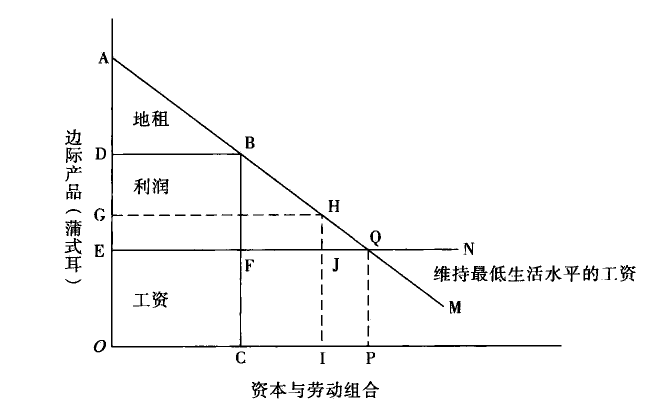
\includegraphics[scale=0.8]{lijiatu.png}
  \caption{\label{fig:lijiatu}静止状态 }
\end{figure}

曲线ABHQM代表了这些边际实物产品。假设距离OC所表示的资本与劳动组合以某一数量投入
到可利用的土地上……所投入的最后一单位资本与劳动组合的边际产品由距离BC表示,模型
中总的农业产量等于面积OABC。李嘉图的问题是确定总产量在工资、利润、地租之间的分配。
李嘉图的分析是灵巧的,因为有三个变量要确定,他通过减法来获得不同份额。正因为这一
原因,李嘉图的收入分配理论经常被称为剩余理论。

维持最低生活水平的工资,通过马尔萨斯人口理论得出,在我们的例子中,假定工资是直
线EFJQN。于是工资率就是FC,总工资是面积OEFC。……需要注意到,利润水平取决于最后
一单位资本与劳动组合的边际产品及维持最低生活水平的实际工资。

\subsection{不同时期的收入分配}

斯密预测,作为劳动、投资以及商品市场竞争的结果,随着时间的推移,利润率将下降。李
嘉图赞成这个观点,但他否认了斯密的所有理由。

斯密的第一个理由与他自己的生产成本价值理论不一致。随着劳动市场竞争加剧和工资上升,
在生产成本价值理论下,没有理由断定利润必定下降。李嘉图通过运用马尔萨斯的人口学说
来反驳斯密,他指出,如果竞争的确抬高了实际工资,那么,人口的增加将在长期中扩大劳
动力的规模,于是工资又将下降到以前的水平。

他通过萨伊定律的主张来反驳斯密关于下降的利润、投资市场与商品市场上竞争的第二个和
第三个理由。李嘉图认为,斯密对利润下降的第二个和第三个解释意味着存在普遍的产出过
剩。其原因在于投资市场的竞争只有在下列条件下才导致利润下降,既不可能按照以前的价
格销售由于新的投资而增加的产量。李嘉图认为,由于新的投资而增加的产量,能够按照以
前的价格销售掉;因此,利润率不会下降。他用同样的主张来反驳斯密关于利润下降的第三
个理由,指出商品市场的竞争不会导致价格总水平下降。在本章末尾,我们将再次考虑萨伊
定律。

李嘉图认为利润将下降,但理由是:早期经济体以高利润和高资本积累率为特征,原因在于
资本积累的源泉是利润。这种资本积累提高了利润率,结果实际工资上升,依照马尔萨斯人
口学说,人口规模将增加。增加的人口要求大量的农业产品……级差地租,地租上升与利润
下降,直至利润率接近为零、资本积累停止。

随着农业利润率的下降,资本将转移,以利用制造业较高的利润率。然而,长期均衡下,整
个经济体中各处的利润率都相等;所以,随着农业中利润率的下降,制造业中的利润率也必
将下降……最终达到所谓的古典静止状态。

利用上图,随着成长的经济体中资本积累与人口增长的发生……如果边际量得到扩展,使OI
表示所投入的最后一单位资本与劳动组合,那么我们会发现,新的更高的地租水平是面积
GAH;利润减少为面积EGHJ;总工资现在是OEJI。随着边际量被推出更远,地租水平提高,
知道总产品只由工资与地租组成、利润等于零为止。这就是静止状态;当OP这么多资本与劳
动的组合被运用时,就达到了这一状态:地租为EAQ,工资为OEQP,利润为零。

\subsection{回到《谷物法》}

尽管李嘉图已经断定,经济体的长期趋势将会导致收入的重新分配,即从资本家流向地主,
然而他之所以反对《谷物法》,是因为它加速了这一过程。因为经济增长的源泉是资本家的
资本积累,所以《谷物法》减缓经济增长速度、加快静止状态到来这一不受欢迎的后果。

李嘉图还提出了第二个主张来反对《谷物法》,即对国际贸易的阻碍减少了世界上所有经济
体的福利。为了了解这一推论,我们必须先来考察他的比较优势学说。

\section{比较优势}

应用于国际贸易中的比较优势学说,明显地体现了李嘉图头脑的极端精明。亚当·斯密对产
品跨国界的自由运动所获得的收益进行了分析。李嘉图拓展了斯密的分析,强调了自由贸易
主张。

用国际贸易理论的术语来说,如果一国在一种商品的生产中拥有绝对优势,另一国在另一种
商品的生产中拥有绝对优势,那么通过专门生产那些生产成本最低的商品,各国都能获益。

\subsection{绝对优势}

通过每单位劳动成本来衡量一国相比它国是否有绝对优势。

\subsection{比较优势}

但是,当一国在所有商品的生产上都更有效率时,又会怎样呢?

% Please add the following required packages to your document preamble:
% \usepackage{booktabs}
% \usepackage{graphicx}
\begin{table}[htbp]
  \centering
  \caption{每单位劳动的产量}
  \label{tab:bijiaoyoushi}
    \begin{tabular}{@{}ccc@{}}
      \toprule
      \textbf{国家} & \textbf{酒(加仑)} & \textbf{布(码)}   \\ \midrule
      英国 & 12 & 6   \\
      葡萄牙& 8 &  1  \\ \bottomrule
    \end{tabular}%
\end{table}

与葡萄牙相比,英国在两个行业都具有绝对优势,两种产品用劳动时间度量的生产成本在英
国都较少。然而,决定国际贸易是否有益的关键因素是比较优势,而不是绝对优势。比较优
势是通过考察每个经济体内部的相对生产力来予以确定的。

在这个例子中,英国在布匹生产上具有比较优势。即在英国,每码布匹新增产量意味着两加
仑酒的损失,而在葡萄牙,为了多获得一码布必须放弃8加仑的酒。葡萄牙在酒生产上具有
比较优势。即在葡萄牙,只用1/8码布的损失,就能多获得一加仑的酒,而英国必须放弃1/2
的布,才能生产出一加仑的酒。

在7.9加仑酒交换1码布与2.1加仑酒交换1码布的价格之间,英国与葡萄牙两个都能从交易中
获益。

依靠比较优势学说,李嘉图证明了,国际贸易收益的决定因素不是绝对优势,而是相对优势。
尽管英国在每个行业都拥有绝对优势,但只要葡萄牙在一个行业拥有比较优势,英国就能从
与葡萄牙的贸易中获益。

在李嘉图关于资源充分利用的假设下,如果要生产更多的任何一种产品,随着资源从收缩性
行业向扩展性行业转义,一些产品的产量必须被减少,多生产的产品的成本,将通过所损失
的产品数量得到度量。

\begin{table}[htbp]
  \centering
  \caption{机会成本}
  \label{tab:机会成本}
    \begin{tabular}{@{}ccc@{}}
      \toprule
      \textbf{国家} & \textbf{酒(加仑)} & \textbf{布(码)}   \\ \midrule
      英国 & 1/2码布 & 2加仑酒   \\
      葡萄牙& 1/8码步 &  8加仑酒  \\ \bottomrule
    \end{tabular}%
\end{table}

然而李嘉图未能考虑问题的另一方面:布和酒的国际价格是怎样的?贸易收益如何在国家之
间分割?在李嘉图使用的例子中,他假设国际贸易中的价格或者说酒和布匹之间的交换比率,
将被确定在最有利于各国的价格中间点上;因此,贸易收益将在两个国家之间被平均分割。
托伦斯也考虑了这个问题,但约翰·斯图亚特·穆勒正确地解决了这个问题,他断定贸易条件
或国际价格,将取决于参与贸易的国家商品需求的绝对力量。

《谷物法》不仅通过收入的重新分配,使收入从资本家流向地主,从而减缓了英国的经济增
长速度,而且减少了所有国家普通公民的福利。比较优势学说揭露了“关税负担是由外国人
承担的”这一流行观点中的谬误。

李嘉图用比较优势理论所证明的是,各方之间的资源贸易或交换,能使双方收益。重商主义
者主张保护行业免受对外贸易侵害,斯密的绝对优势原理使之受到损伤,比较优势学说则几
乎将它推翻。更重要的是,该学说也表明,即使由于相对稀缺性而使社会上存在冲突,然而
经济参与者之间的资源交换,将导致更大的总产量和共有的收益。

\subsection{李嘉图、斯密以及贸易基础}

在比较优势主张下国内或国际贸易的发展为市场体制的发展提供了强大的推动力,个体能够
追随他们的自我私利,加入到自愿的而有共同利益的交换中,这种交换也有益于整个社会。
然而,从另一个角度来看,比较优势主张的出现,非常有悖常理地阻止了经济理论的发展,
因此也阻碍了问我们对经济体的理解。原因在于,李嘉图的比较优势主张依赖于如下假设,
即个体与社会的相对生产力都是既定的与固定的。经济学家将这种固定的和既定的变量称作
“外生的”,表明他们的价值是在特定模型的结构之外决定的。比较优势模型显示了从贸易
中获得的好处,因此,它在定位上是静态的。

当我们考察亚当·斯密的开放与自由贸易主张时会发现,其绝对优势观念的基础是一种动态
的而非静态的设想,即随着时间的发展,劳动分工将导致生产力提高。专业化与劳动分工将
导致较高的生产力。将斯密的这个见解应用于国际贸易时,人们可能会指出,今天没有显示
出比较优势的两个国家,通过实行专业化,尤其是生产过程的专业化,能够随着时间的变化
而发展出比较优势来。直到20世纪后半期,经济学家才着手发展这种动态的贸易理论,其中,
内生决定的收益递增开始出现。

斯密与李嘉图对贸易基础的不同理解,反映了他们不同的方法论。斯密是一位运用前后关联
的分析来发展其经济政策的大师。李嘉图比斯密拥有更加抽象的方法和更加非关联的政策方
法,他也非常擅长经济学艺术。李嘉图运用劳动价值理论、比较优势模型及其他同样抽象的
假设,缺乏前后关联的基础。其模型推断,自由实现的资源交换将增加经济馅饼的规模。显
然,从斯密与李嘉图的例子中可以看到,经济政策艺术可以为拥有不同方法倾向的经济学家
所精通。

\section{资本主义经济体的稳定与增长}

李嘉图与马尔萨斯之间对资本主义体制保持资源充分利用能力的争论,极大地影响了经济理
论的发展。在经济文献中,这一争论被认为是对萨伊定律的争论。李嘉图赢得了这场争论;
从那时直到20世纪30年代凯恩斯发展了其宏观经济理论并批评了李嘉图的观点为止,正统经
济理论很少关注由萨伊定律引发的问题。萨伊定律的实质是,资本主义体制将自动实现资源
的充分利用和较高的经济增长速度(马克斯认为萨伊定律实则建立在物物交换基础之上)。
李嘉图、詹姆斯·凯勒以及萨伊赞同这一立场,马尔萨斯对他进行抨击。

\subsection{重商主义者的总需求观点}

大多数重商主义者认为,个人的借鉴与储蓄友谊与国家。然而,一些人,例如曼德维尔则提
出,储蓄引起失业,较多的消费支出将增加经济活动,并因此使经济体受益。曼德维尔主张,
繁荣与就业是通过支出,尤其是奢侈型的消费支出得到增进的,并且储蓄对于经济体是有害
的,原因在于它较低的产量与就业水平。

\subsection{斯密的总需求观点}

斯密否定了曼德维尔以及具有相似意向的重商主义者的观点。他赞扬节俭与储蓄;根据他的
分析,资本积累才是繁荣与增长的主要决定力量。他提出,消费不足主义者认为消费不足将
导致衰退和低增长速度,他们错认了形势,原因在于他们未能了解储蓄与投资过程以及这一
过程对经济体的影响。对斯密来说,储蓄并没有减少总需求,仅仅使需求从消费产品改为投
资产品。

\subsection{马尔萨斯的消费不足主义}

马尔萨斯《政治经济学原理》

斯密断定,经济进步取决于劳动力的规模与效率、自然资源的数量与质量、制度结构以及资
本积累的数量,他认为资本积累是决定经济发展的关键因素。李嘉图也将资本积累视为一个
国家财富增长的主要源泉。这一分析仅基于总供给一方:增长只收到一个国家劳动、资本以
及自然资源供给增加程度的限制。但是,如果最终产品的总需求小于总供给,产出量少与资
源充足利用时的产量,或者说出现衰退,那么情况将会怎样呢?

曾经提出过消费不足或过量生产可能性的少数重商主义者,因斯密对他们立场的反驳而受到
有力压制。不过,在19世纪早期,这一问题再次被提出。劳德戴尔伯爵、西斯蒙第等质疑了
经济体自动引起资源充分利用的能力。1820年,马尔萨斯提出了这些问题,1936年版《原理》
第2篇中,他提出有必要考察需求一方,或者说他所称的“有效需求”。马尔萨斯从未精确
地陈述他使用的有效需求是什么含义,他对萨伊定律所引发的问题的理解,也的确令人困惑。
但是,他意识到保持资源充分利用存在着困难,尽管他还没有清楚地掌握这些困难的准确性
质。

他的比较天真的主张是,劳动者没有获得全部产品,因此,单独就劳动者需求而言,不足以
按照满意的价格购买全部最终产品。马尔萨斯接受了下面的这种观点,即储蓄并不意味着贮
藏,储蓄将作为投资支出流回到市场上。有时他主张货币的其它功能,质疑李嘉图关于货币
仅是一种交换媒介,没有人滞留购买力的观点,但是他从未将这些简介发展成对衰退的一种
货币解释。

他对经济体某些问题也有比较成熟的见解,他主张“储蓄--投资”过程无法无限期地继续下
去而不导致长期停滞。存在一个经济体能够吸收的适宜的资本积累率,过多的储蓄与投资将
引起难以应付的问题。储蓄过程导致消费产品需求减少,投资过程导致未来更多的消费产品
的生产。此外,马尔萨斯意识到要保持资本主义体制中资源的充分利用,总产量水平和总消
费水平一定要保持扩张。

马尔萨斯断定,因为劳动者与资本家方面存在不充分的有效需求,所以,一定要通过社会上
那些只消费不生产的人来填充缺口。这些非生产性的消费者就是那些提供服务的人(教士、
教师、仆人、公务员以及其他人)和地主。这样,地主的社会作用之一就是不生产而消费,
从而有助于防止衰退和经济体的最终停滞。

\subsection{萨伊定律}

正统古典经济学家拒绝接受劳德戴尔、西斯蒙第以及马尔萨斯的批判。他们的观点得到萨伊、
詹姆斯·穆勒以及李嘉图有力而明确的认同与发展,他们主张,在生产产品的过程中产生了充
足的购买力,能按照满意的价格将这些产品带离市场。过量生产或者他们所谓的供过于求可
能发生在特定市场,但是整个经济体不可能有普遍的过量生产。经济活动总体水平的下降,
将只持续一个较短时期,原因在于,市场会自动地将经济恢复到资源充分利用的状态。因此,
古典学者强调,在长期中不存在过量的资本积累。

经济体的年产值,作为购买力被经济体成员获得。于是,总能够产生充足的购买力,把生产
出的产品带离市场,这不会有什么问题。此外,古典学者认识到,在特定市场上需求与供给
不可能相吻合,可能存在特定商品的过量生产——某一特定行业的超额供给。特定行业的这种
供过于求,是市场力量作用于需求方或供给方的一种表现。但是,一个行业的超额供给,意
味着必定存在对另一个行业产品的超额需求。在一个存在可变价格与资本流动的经济体中,
生产要素将离开具有超额供给的行业,流向具有超额需求的行业。因此,在长期中,能够保
证所有资源的充分利用。

尽管产生了充足的购买力,将所有生产出来的商品带离市场,然而,有什么来保证这种购买
力在市场上得到实现呢?萨伊定律所蕴含的答案,经常被简单地表述如下:供给创造出他自
身的需求。供给创造潜在的需求,这不会有什么问题,但是,关键的问题是,潜在需求是否
能够作为有效需求在市场上得到实现。李嘉图、詹姆斯·穆勒、萨伊通过简单地做出下面的
断言来处理这一问题,即所有潜在购买力都会作为消费者产品或生产者产品需求回到市场上。
实质上,他们回到了斯密储蓄决策即投资决策的观点上。他们否认贮藏的可能性——没有人将
黄金锁在箱子里。在他们的体系中,货币只是一种交换媒介;因此,他们否定衰退或停滞的
任何可能的货币原因。然而,马尔萨斯从未清楚地认识到这些难点。在接受理论检验所必需
的全部假设的同时,他又试图反驳理论本身,从来没有能够阐明这一见解,形成合理的批评,
或者发展另一种可替代的关于收入水平与经济增长速度决定因素的理论。

\subsection{关于金银的争论、亨利·桑顿以及李嘉图的货币理论}

李嘉图对萨伊定律的看法,是在发生于19世纪早期的争论中得到发展的——“金银争论”;争
论的焦点是拿破仑战争期间通货膨胀的原因是什么。金银通货主义者主张,通货膨胀的原因
是发生在战争期间的货币扩张。反金银通货主义者则认为,如果不包括诸如歉收这类实际原
因,通货膨胀的原因是比较复杂的。他们赞同真实票据学说(Real Bills Doctrine),该
学说主张如果货币发行涉及短期金融商业操作(例如存货融资),则不会有货币的过度发行。
当货币增加不超过实际交易需要时,通货膨胀的原因就不在货币部门。罗伯特·托伦斯是反
金银通货主义者观点的主要支持者——《论货币与纸通货》。

李嘉图很快就成为了金银通货主义者观点的主要说明者,这一观点类似于今天现代货币主义
者的观点——通货膨胀总是一种货币现象。对李嘉图而言,经济体中的“活动”是在实际部门;
货币只不过是隐藏在实体经济后面的一层面纱;他在争论中的作品就是用来揭开那层面纱的。

李嘉图的威信使其观点遮蔽了亨利·桑顿的观点。他是一位非常敏感和有思想的经济学家,
著有《大不列颠的票据信用》。桑顿通过利息率和银行的贷款实践来探寻货币的影响,在此
过程中,他意识到影响实体经济的货币非均衡的可能性,从而意识到货币影响实体经济。对
桑顿而言,货币不仅仅是一种面纱。在其讨论中,他甚至认识到实际利率与名义利率的区别。
但可惜的是,他从这些较成熟的观点中退出了,使得被认为是标准的古典货币理论停留在过
于简单化的基础上,并以李嘉图版本的货币数量理论——面纱——为中心。

\subsection{技术性失业}

1821年出版的《原理》第三版中,李嘉图加入了论机器一章。之前李嘉图分为劳动节约型机
器的使用不会减少对劳动的需求,“论机器”中,李嘉图声明:“劳动阶级认为采用机器往
往有损于他们的利益的看法并非基于成见和错误,而是符合于政治经济学正确原理的。”。

就像前面的引语所暗示的那样,李嘉图对技术性事业可能性的讨论,与他关于不可能存在普
遍供过于求的观点不相一致。他认为,如果最新使用的机器,是通过将流动资本转换成固定
资本来筹集资金的,那么工资基金将会减少,事业将会产生。

\subsection{凯恩斯伦马尔萨斯与李嘉图}

人们现在对马尔萨斯与李嘉图之间就萨伊定律所作争论的关注,以及对马尔萨斯除人口论题
外其他经济观点的关注,在很大程度上源于凯恩斯所作的《传记文集》(Essays and
Skeches in Biography)以及《通论》。凯恩斯提出了三个相关的问题:(1)关于萨伊定
律的“马尔萨斯——李嘉图争论”;(2)适合于经济学的方法;(3)在这两个问题上李嘉图
对马尔萨斯的胜利,对经济学作为一门学科后来发展所产生的影响。

\begin{quotation}
李嘉图胜利的完整程度始终是出乎意料和难以理解的事情。看来一定是由于在一系列事物上
他的学说能适合该学说所存在的社会的要求。我设想,该学说所得到的结论和没有经济学知
识的普通人所预期的结论具有很大不同之处给他带来智慧上的威信。它的教言在实践上的严
酷和难以接受反而使它具有优越性。它的可以被作为宏大而符合逻辑的上层建筑的基础使它
具有学术上的瑰丽。它能把社会上的许多不公正之处和明显的残酷事实解释为在进步中不可
避免的后果,以及把改变这些事态的企图解释为弊大于利的事情使它受到统治者的赞赏。它
为资本家们的自由行动提供理论根据,使它能得到统治者背后的主要社会力量的支持。(高
版《通论》38页)
\end{quotation}

在关于马尔萨斯的短文中,凯恩斯赞扬马尔萨斯能够理解经济体保持充分就业的困难,他引
用马尔萨斯给李嘉图的信“来表明马尔萨斯完全理解了超额利润通过它对利润的影响而影响
产量。”经济思想史学家承认,凯恩斯大大曲解了马尔萨斯关于经济体无力实现充分就业的
含糊观点。尽管马尔萨斯的直觉可能是正确的,但是,他对李嘉图的批评是含糊的和不完善
的,并且就像凯恩斯所正确注释的那样,他没有提供一种可替代的理论解释来代替萨伊定律。

尽管马尔萨斯《人口原理》第一版是严格演绎的,但是第二版以及后来的版本却更加归纳。
凯恩斯坚定地赞成马尔萨斯的方法,批评李嘉图的抽象模型。……凯恩斯给予马尔萨斯和其
他人进一步的赞扬,认为他们“这些人凭借着他们的直觉,宁愿对真理作出模糊的和不完整
的认识,但绝不坚持错误的看法;而那种来自简单逻辑推理的错误说法固然明白准确,固然
前后一致,但却建立在不符合事实的假设前提之上。”(高版 《通论》385页)

凯恩斯观点的困难在于,它以一种后见之明呈现出来……马尔萨斯的观点使部分非生产性消
费者,尤其是地主的利益合理化;后者的观点使资本家的利益合理化。其它机构将有可能替
我们回答这个问题——正如凯恩斯所主张的,公认的观点一定拥有“权威身后占优势的社会力
量的支持”。

\section{总结}

19世纪的第一个二十五年为经济理论带来很多新贡献。唯一具有可比性的另一个重要短时期
是20世纪30年代。在那个时候,大萧条将经济学家的注意力转向了一些新的问题。李嘉图使
经济学的范围从几乎专门关注经济增长问题,转向包括不同时期收入功能性分配变化问题。
李嘉图对收入分配的关注,使他与以前的经济学家相比,将更多的注意力放在阐明价值理论
或相对价格的微观经济问题上。……他对萨伊定律和货币数量理论的捍卫,也使某些宏观问
题的考察,从后来的古典正统经济文献中被成功地排除掉。

李嘉图代表了从斯密方法——理论与历史描述的松散结合,转向高度抽象的经济模型方法的明
显突破。


%%% Local Variables:
%%% mode: latex
%%% TeX-master: "../../main"
%%% End:

\chapter{约翰·斯图亚特·穆勒与古典经济学的衰落}

穆勒是一位天才的与众不同的思想家,对经济学、政治学和哲学都作出了重大贡献。他巨大
的思想力,是通过他父亲詹姆斯·穆勒的高广度和强度的天才精英教育而实现的……其心理
代价是穆勒二十岁时表现出来的精神抑郁,所幸的是,经过一段时间的消沉之后,穆勒重新
恢复了健康,并成为他所处时代以及所有时代中最主要的知识分子之一。

穆勒实质上是一位社会哲学家,他下决心要提高个人在社会中的作用。与他父亲和李嘉图的
悲观主义不同,他提出了保守的乐观主义,预期了一个良好社会的发展。他经济思想的主要
来源有:早年在斯密、李嘉图、他的父亲及边沁古典经济学方面所受的影响;傅立叶和圣西
门的社会主义著作;孔德的著作(他使穆勒将经济学仅仅视为人类社会行为的一个方面);
最后是穆勒的朋友哈里特·泰勒,她后来成了他的妻子,人文社会主义。穆勒既是一位古典
自由主义者,也是一位社会改革家。他认为他的主要任务是写一本对李嘉图的学术思想进行
清晰说明的书,并将19世纪第二个二十五年期间出现的新观点融合进去。然而,穆勒是一位
对国际贸易理论以及对“供给——需求”分析作出了重要贡献的原创思想家。

穆勒的《政治经济学原理》代表了对古典经济理论的最大修正,也代表了古典经济学理论的
顶点。当时对李嘉图有很多批评,穆勒对这些批评作出了回应。这些批评有三个主要来源。
第一,越来越多的证据显示,李嘉图学说与从英国经济体运转中获得的经验结果不一致。马
尔萨斯人口理论是李嘉图体系的一个实质性前提,与之相反,不断增多的证据表明,随着人
口增加,实际人均收入提高了,而不是减少了;并且,农业中技术的进步,使农业正经历着
收益递增而不是收益递减。第二,学者们开始彻底研究李嘉图的理论结构,尤其是他的劳动
价值论,并且发现李嘉图对需求的处理,以及对利润在价格决定中作用的处理是欠缺的。第
三,许多人道主义者和经济学家,忽视经济思想的技术内容,猛烈抨击李嘉图理论结构所代
表的新兴资本主义经济体的基础。

经济思想后来的很多发展都出自于对萨伊、李嘉图等长期供需均衡的批评。此外,由法国、瑞士、
德国以及英国经济学家创造的越来越多的社会主义文献集,对古典观点——依靠资本主义经济
体不受阻碍地运转,能完美地实现经济和谐——提出了质疑。

批评中更加技术性的内容,多是那些把经济学作为主业而不是作为副业来研究的人提出的。
他们的主要目标是部分地否定马尔萨斯的人口学说、历史上的农业收益递减以及工资基金学
说,并且用他们的理论来代替劳动价值理论。在他们的价值理论中,利润是决定价格的因素,
需求与效用在相对价格决定中的作用被扩大了。这种分析形势最终接触了边际效用学派和阿
尔弗雷德·马歇尔经济学的果实,前者始于19世纪70年代。

\section{李嘉图之后经济学的发展}

\subsection{对古典经济学的早期批判}

很多早期古典经济学的批评家将19世纪西欧资本主义的运转视为不和谐。大部分批评者都提
倡用非暴力手段消除社会冲突,尽管所开出的治疗药房随着经济学家的不同而不同。早期社
会主义者间接影响了正统理论的发展,却直接影响了穆勒,尤其是对英国立法和工人运动的
形成产生了重要作用。“实际上,19世纪30年代的大多数理论发展,尤其是涉及把利润的性
质当做一种收入来源的理论,都或多或少是有意识地反对传播社会主义意识形态的结果。”

\subsection{经济学的范围与方法}

李嘉图转从斯密理论与历史描述的松散结合转向抽象演绎的理论模型,很少直接论述方法问
题。但是,他后来的追随者就经济学的适当方法达成了几乎完全一致的看法。他们的新李嘉
图方法将经济学看做是一门基于某些简单假设的学科。因此,经济学家的任务是纠正体系的
逻辑,以确保结论是根据既定假设得出来的。在后李嘉图时期,当经济理论与可利用的经验
数据之间出现冲突时,这样一种方法观点及其有助于经济理论的发展,其原因在于,他使
经济学家可以忽视数据。

在此期间,涉及经济学范围和方法的最佳并且是最清楚的两个论述,是由拿骚·西尼尔和穆
勒作出的。在《政治经济学大纲》中,西尼尔将政治经济学界定为处理“财富的性质、生产
以及分配”。西尼尔认为,经济学家已经浪费了时间去试图收集更多的经验信息,应当位经
济学家确定努力的方向,即提高经济理论的逻辑一致性。

西尼尔指出,作为一门科学,经济学的基础依赖于四个基本主张:(1)理性原理,即人们
是理性的和精于计算的,并且希望以最小的牺牲获得财富;(2)马尔萨斯人口学说;(3)
农业收益递减原理;(4)历史上的产业收益递增原理。将经济学视为纯粹演绎性学科,对
经济理论的发展具有重要影响;但在考察这些后果之前,我们先着眼于细腻而方法论观点中
另一个引人注意的方面。

西尼尔是明确主张经济学应当是实证科学的最早的经济学家之一。他认为作为一个科学家,
经济学家应当注意区分规范判断与市政经济分析。例如他在以下两者之间所做的区别:(1)
支配财富性质与生产的一般法则;(2)支配收入分配的原理,它反映了经济体的特定习俗
和制度结构。穆勒后来就生产法则(是像引力定律一样的自然法则)和作为其体系基础的分
配法则(不固定,来自于特定的社会与制度安排)作了区分。西尼尔主张,作
为一个科学家,经济学家能够指出各种经济行为的后果,或者达到既定目标的可能途径,但
是,他或她不应当离开实证科学分析的领域,不应对既定活动形式上的要求作出价值判断简
单地说,经济学家应当是他或她关心“是什么”“而不是应当是什么”。经济学家的“结论,
无论其一般性和真相是什么,都不允许他增添一个字符的建议。”

认同李嘉图所实践、细腻而所阐述的方法,对李嘉图之后的经济学产生了不幸的影响。19世
纪30到40年代变得明显的理论与现实之间的冲突,在很大程度上被忽视了;尽管经验证据与
李嘉图理论体系的几个基本前提相矛盾,然而,经济学家还是顽强地坚持着李嘉图的模型。

\subsection{马尔萨斯的人口理论}

李嘉图的《原理》出版后,深切关注人口问题的经济学家为避免马尔萨斯人口论中过量人口
严重后果问题,主张家庭使用一些避孕措施。

西尼尔认为,历史证明表明食物供给人口比人口增加得更快。

\subsection{工资基金学说}

作为一种短期工资理论,工资基金学说简单地主张,工资率取决于劳动的供需。他们实际上
不是现代经济学中使用的供需。工资基金的规模是积累的资本中支付给劳动的部分,它使劳
动需求固定。给定工资基金的规模,短期工资率就通过用劳动市场上的人数除工资基金而得
到。于是在短期中,工资基金在量上是固定的,劳动数量是固定的,工资率被唯一地确定下
来。

随着马尔萨斯人口理论的远去,工资基金学说不得不承担起作为短期和长期工资理论的重担。
这是它不可能做到的,原因在于,工资基金学说中没有一处说到有关劳动的长期供给的内容。
在这一时期的经济学家的著作中,似乎对工资基金学说的看法与对劳动工会的态度之间没有
什么联系:主张工资基金学说的很多经济学家其实明确赞成组成劳动工会。不过,在通俗文
献中,工资基金学说是以反对通过工会的经济主张而知名的。穆勒于1869年对工资基金学说
作出了著名的否定,并且后来的经济学家对穆勒的这一否定赋予了重要性。

\subsection{历史上的收益递减}

对英国的经济来说,所有可以利用的数据都表明,李嘉图基于历史上的收益递减的预测是错
误的。马克·布劳格被一些人认为是对这一时期进行研究的最精明的现代学者。他曾说道
“理论与现实之间的分离,可能从来没有比在李嘉图经济学全盛时期更加彻底。”……这种
分离根植于李嘉图的方法论中,为李嘉图所实践、西尼尔所揭示的方法论,专门强调从一组
既定的假设中进行推理的演绎过程;因此,它使李嘉图主义者忽视他们的模型与是时间的矛
盾,而使自己忙于完善其理论结构的优雅型。大多数非正统经济思想的一个共同点是:他们
都认为,正统经济理论精确地显示出李嘉图经济学的缺陷——正统模型与事实之间的冲突以及
完善其理论结构的演绎过程和内在一致性所收到的困扰。

\subsection{未采取的道路:查尔斯·巴比奇与收益递增}

巴比奇是以机械计算器的发明者而知名,但他也是一位敏锐的经济观察家,他写了一本比李
嘉图著作要好得多的书,描述大量生产的性质与含义。内森·罗森伯格指出,巴比奇捕捉到
了通过重复劳动和大量生产能够实现的成本节省,并且看到收益递增将成为行业的驱动力,
巴比奇能被视为现代产业经济学复杂方法之父。

\subsection{下降的利润率}

按照李嘉图的观点,农产品的成本增加时,边际土地上的利润随着边际内土地地租的提高而
下降,这一趋势将会持续下去,知道利润率接近为零,并且因收入由资本家向地主的再分配
而产生静止状态。但是,这一断言的正确性也只能通过经验证据而不是理论得到确定。度量
不同时期经济体利润率变化的统计问题相当有难度,19世纪也没有这种度量所要求的统计工
具。当然,一些经济学家也质疑今天是否拥有这些统计工具。尽管缺乏对历史上农业收益递
减以及对利润率下降和静止状态最终到来的经验证明,但是李嘉图主义者——尤其是穆勒——仍
然坚持这些预测。

\subsection{利润(利息)理论}

李嘉图断定,利润率的变化对于解释不同时期相对价格的变化所起的作用并不重要。她认为,
尽管相对价格在理论上取决于劳动成本和资本成本,资本成本为利润,然而利润在实际中所
起的作用如此无关紧要,以至于能将它们忽略掉。可见,李嘉图的价值理论实际上就是生产
成本理论,只有劳动一种成本。

李嘉图式社会主义者利用李嘉图的劳动价值理论来表明劳动承受着剥削……恰恰是为了纠正
李嘉图价值理论的逻辑缺陷,并支持盛行的意识形态反对李嘉图式社会主义者的进攻,使得
经济学家们将他们的注意力转向了利润。

在后李嘉图阶段的早期,对利润理论和价值理论最重要的贡献是由拿骚·西尼尔作出的,他
最先试图发展一种利息节欲理论(abstinence theory of interest)。西尼尔在他的价值
理论中,比李嘉图更强调需求方面的效用;在论及供给方面时,他又强调以无效用作为实际
生产成本。利用古典经济学的基本心理假设,他主张人们都是理性和精于计算的。如果我们
要生产资本产品,一些人就一定要放弃消费,除非因这一痛苦而给资本家以报酬,否则他们
不会放弃消费。因为资本与劳动两者对最终产品的生产都有必要,所以他们的价格必定足以
支付这两种实际生产成本。因此,西尼尔发展了一种生产成本价值理论,其中工资是对劳动
的返还,利润是对资本供给者的返还。

古典经济学没有对利润与利息进行区别。西尼尔致力于发展一种利息理论,该理论成为19世
纪末期发展起来的庞巴维克理论的前身。西尼尔遵循着古典惯例,他所进行的讨论只涉及供
给方面。他仅考察了储蓄供给曲线的决定力量,而利息理论也应当解释对投资的需求。作为
一种反对社会主义者的主张,西尼尔的利息结余理论存在几个缺点。他主张储蓄的供给曲线
是完全有弹性的,并且储蓄所招致的痛苦成本或者说无效用,对于富人和穷人来说是相同的。
因为他专门将利息看成是对痛苦成本或者说是对放弃消费的无效用的支付,所以通过遗产或
赠送而获得的资本的利息收入,就没有牺牲社会公正或经济公正。因此最后,就利息的社会
公正而言,西尼尔的利息理论所提出的问题,可能比它回答的问题还要多。

\section{穆勒思想的背景}

\subsection{穆勒的经济学方法}

他把经济学当做使用演绎方法的假设科学。经济学家作出某些假设,然后从这些假设中演绎
出结论。因为实验方法对经济学家来说不可用,所以他们必须依靠演绎技术,而不能运用自
然科学中非常富有成效的归纳技术。然而,穆勒小心地指出,经济学家从其演绎模型中得出
的结论,应当通过与事实的比较予以经验。按照穆勒的观点,应用演绎模型预测的结果与历
史事实之间缺乏一致性,这显示出重要的却未被注意到的“干扰原因”。这些原因可能会导
致新的更多的假设,这些假设再通过演绎推理产生新的结论,或者它们可能是经济学家未考
虑到的非经济因素的结果。

经济学家假定了一个抽象的经济人,完全受着拥有财富欲望的激励。然而,穆勒认识到,尽
管这种抽象产生了一些有用的结论,但它最终还要与更加复杂的人类社会与人类活动模型相
结合。

西尼尔区分了实证经济学与规范经济学,目的是将规范性的判断从经济研究中消除掉,穆勒
吸取了这一划分,目的却是将社会哲学问题并入到李嘉图模型中。

在《自传》中,穆勒论述了其生产法则与分配法则概念的来源,他的主要灵感源自于印证圣
西门主义者的社会主义著作,穆勒证实哈里特·泰勒是使它确信区分生产法则与分配法则之
重要性的人。李嘉图理论对静止状态的预测,尤其是其中有关工资将停留在维持生活的最低
水平上的预测,遭到穆勒更加乐观态度的反对,穆勒深信随着时间的变化,社会将以一种贤
明而人性的方式来行动,所以将会产生更加平等而公正的收入分配。穆勒赞成高遗产税,但
反对累进税,原因在于他担心累进税的阻碍效应。他也提倡形成生产者合作,并且认为当工
人不仅获得工资,而且从这些合作中获得利润和利息时,他们将会有更大的动力来提高生产
力。此外,他认为农业收益递减可以通过增加对人的教导以及晚婚和节育来降低人口率。

现代正统经济理论揭示了生产法则与收入的功能性分配之间的密切关系。最终产品与服务市
场零售价格的决定力量,与各种生产要素价格的决定力量密切相连。投入与产出之间的实物
关系被经济学家称作生产函数,它决定了不同生产要素的边际实物生产力,并且一种生产要
素的市场价格部分地由这一生产力来决定。然而,关于个人收入分配的决定力量,现代正统
理论只有很少的阐述。个人收入分配取决于一组更加宽泛的非经济变量,如一个社会的法律、
习俗以及制度安排,因此按照正统经济学的观点,个人收入分配在经济学学科之外。此外,
正统理论家不愿意考察与个人收入分配相关的问题,原因在于它涉及规范性问题和价值判断
人。如果将穆勒的理论转换成现代经济理论术语,那么穆勒将会主张在不同要素的边际生产
力与个人收入分配之间,只存在一种松散的联系。社会不能修正生产函数,但是社会确实有
能力实现一种与其自身价值判断相一致的个人收入分配。

\subsection{穆勒的折衷主义}

穆勒的巨大实力是他的折衷主义,这也是两位最重要的后穆勒主义英国经济学家马歇尔与凯
恩斯的实力。

\subsection{杰里米·边沁的影响}

穆勒及其同时代的人致力于将理论与政策相结合,对他们影响最大的是英国人杰里米·边沁
的著作。1780年,边沁第一部重要著作出版之后,他便成为了一群改革者的智力领袖,这群
人以哲学激进分子或者说功利主义者而著称。马尔萨斯之前,边沁就主张节欲;边沁主义者
后来曾提倡一连串改革,包括全民投票(含女性)、监狱改革、言论和出版自由、文职以及
工会合法化等。边沁从一个简单前提开始,即人们受到两种强烈欲望的激励:获得愉快和避
免痛苦。如果社会能够度量愉快和痛苦,那么就能创造出导致多数人的最大幸福的法律。按
照边沁的观点,度量愉快与痛苦的最佳办法要借助于货币指标。因此,边沁及其追随者希望
设计出导致多数人的最大利益的法律,从而使社会改革成为一门精密科学。

然而,穆勒也部分地否定被他父亲所接受的边沁主义的某些方面。在他生命的剩余时间里,
在避开边沁理论结构某些方面的同时,他也继续分享边沁对社会改革的关注。边沁主义体系
中的两个部分格外扰乱他。首先是其中的教条主义,尤其明显的是,哲学激进主义者坚决主张快乐主义
的愉快——痛苦计算,能够被用来分析所有的人类行为。受到孔德和其他人的影响,穆勒不能
接受这样一种狭隘的观点,这一观点似乎忽视了将人类和其他动物区分开的很多因素。第二
个干扰是,在某些方面,激进主义者并不足够激进。

\subsection{自由放任、干预抑或社会主义}

这种分类很难适用于穆勒。也许,表现像穆勒这样敏感而复杂的思想家特色的最好方式是认
为在公共政策方面,他代表了古典自由主义与社会主义之间的一个中点。他的社会主义不是
马克思主义的,并且穆勒显然与马克思有很少的联系。然而,他的确区分了革命社会主义者
(左翼革命的)与哲学社会主义者(右翼进化的),他自己的观点似乎更倾向于后者。

穆勒在他的短文《论自由,1959)中,试图表述政府与公民之间的适当关系。一些强烈的古
典自由主义成分包含在内:当政府反对个人意愿时,唯一正当的权力行使是“阻止伤害其他
人。他自身的利益,无论物质上的还是精神上的,都不是充足的理由。”然而,《原理》中
他又有些异常。在对实际社会行为的讨论中,穆勒又被迫放弃了这种强烈的自由主义观点,
他在一般规律的例外上发现了异常。在《原理》中,他有一处作了有力的自由主义陈述,
“总之,自由放任应当是通用的惯例:除非为一些巨大利益所要求,否则对它的每种违背都
是某种罪恶。”另一处他又逐渐从严格的自由放任观点中退出,声称“政府的唯一目的是保
护个人和财产,这是不能接受的。政府的目标就像社会联盟的目标一样广泛。它们由所有的
有益行为以及所有对罪恶的免疫力组成,这些都是政府的存在所能直接或间接给予的。”换
句话说,穆勒承认政府干预的缺失不一定必然导致最大的自由,因为对自由来说,存在很多
其他限制,这些限制只有立法或者政府才能消除。

穆勒对地主的谴责是尖锐的,他的政策建议是从地主那里拿走地租和土地价值的额外增加额。
穆勒并不强调劳动者与社会其他成员,尤其是资本家之间的阶级冲突;然而,其全部社会哲
学和他所提倡的主要项目,例如全民教育、借助遗产税的收入再分配、工会的组成、工作日
的缩短以及对人口增长率的限制,都暗示着除了那些与土地所有权相联系的冲突与不和谐之
外,体系中还存在着其它的冲突与不和谐。

穆勒对私人财产的论述,反映出他将古典自由主义与社会改革相混合。财产权不是绝对的,
当社会断定财产权与公共利益发生冲突时,它能够废除或者改变这些权利。

就像他否定社会主义者所认为的私人财产是社会罪恶的主要原因一样,穆勒也不能接受社会
主义者所认为的竞争是导致社会困难的一个原因。“对竞争的每一种限制都是一种罪恶,对
竞争的每一种扩充,即使暂时伤害性地影响到一些劳动者阶层,但最终也总是有益的。”穆
勒对竞争的这些赞同观点,与他对工会的支持及其通过使用垄断力量改善劳动者状况的其他
尝试之间的矛盾,给他带来而一些难题。工会“远不是对自由劳动市场的一种妨碍,反而是
自由市场的一种必要手段;是使劳动的销售者能够在竞争体制下,正当地招股自身利益的一
种不可缺少的办法”。

\subsection{一种不同的静止状态}

穆勒的折衷主义和他带给经济学的人道主义,没有一处比在对经济体长期趋势的论述中得到
更好的反映了。尽管经验证据相反,穆勒仍然坚持基本的李嘉图模型,该模型预测了利润率
下降与静止状态。但是,穆勒的静止状态不是李嘉图所预想的那种消沉。与到目前为止几乎
所有的正统经济学家相反,穆勒不能确信经济处于成长中的国家,例如他所处时代的英国是
否是一个理想的居住地。穆勒发现,一个繁荣的成长的经济体存在很多应受责难的方面,例
如“踩踏、挤压、推搡以及践踏”。在著名的有关静止状态一章中,穆勒以批评的眼光来看
待他自己的社会,并勾画出他对未来的希望。穆勒对美好社会所设定的标准是个体幸福、福
利的提高。他明确地表示,这些东西不一定用物质产品来度量。产量增加和人口增加本身不
一定是有益的,也不能自动地有益于社会。按照穆勒的观点,静止状态可能是非常渴望的一
种社会形态,随着经济活动的步伐放缓,更多的注意力将被集中在个体上以及他的非经济和
经济福利上。“只有在世界上落后的国家,增加人口还是它们一项主要目标;在那些最发达
的国家,经济上需要的是一种更好的分配。……在没有一个人贫穷,没有一个人希望更加富
有的同时,也没有任何理由担心,其他人向前的努力会把自己向后推。”

\subsection{穆勒的社会哲学}

\section{穆勒的经济学}

\subsection{理论的作用}

由于受到正统与非正统思想家著作的影响,穆勒总是批评地对待技术性的经济理论。理查德·琼
斯《略伦财富的分配>1831年版,一般性地批评了古典观点,并特别批评了李嘉图的地租理
论,因为他们的分析忽视了经济体的历史与制度环境。琼斯被称作历史学派的先驱者,他质
疑李嘉图的分析在所有时间和所有地点的应用,并提倡用一种更加经验性的方法来解释制度
结构的变化。穆勒的《原理》第2篇第4章“关于竞争与习俗”部分,含蓄地认可了琼斯的这
一批评,这表明穆勒认识到,抽象的经济理论必须通过历史上盛行的制度的了解来加以调和。
因此,穆勒主张竞争与习俗两种力量支配着收入分配。“在所有场合,他们(英国经济学
家)都倾向于表达自己的思想,好像他们认为竞争实际上其作用一样,而不管竞争起作用的
趋势显示出什么。”

穆勒采取了一种相对的历史观点,指出市场经济中竞争发生作用是一种有较少经验的历史现
象,如果我们回过头看就会发现,习俗传统在解决有关收入分配的经济问题上起着主要作
用。……他认识到李嘉图体系假定经济体中存在一组参与者即生意人,他们被获取利润这一
强烈欲望激励着,正是通过他们的活动,资源得到配置,市场达到了均衡。然而,也有不存
在这一类参与者的经济体,即使是市场经济,如果其中“缺乏有魄力的竞争者,那些拥有资
本的人也宁愿把它留在原地,以一种更宁静的方式通过资本获得较少的利润”。此处,以及
在他书中的其他地方,穆勒一直在考虑一个问题,即应当给与抽象理论多大的重要性,又应
当给予制度的--历史的材料多大的重要性。这一问题被不同的非正统经济学家一次又一次地
提出来,今天仍然有待于我们去解决。

一些社会力量,如习俗修改其至否定了基于竞争性过程的预测,面对这样的社会力量,经济
学家为什么还要不断地使用竞争性模型?“如果我们认为只有通过竞争原理,政治经济学才
能具备科学的特性,那么这就可以得到部分的理解。”但只有当我们接受对科学的下面这种界
定时,这一奇怪的结论才有意义:经济理论或模型要想是科学的,就要能够得出严格的且准
确的结论。换句话说,科学要求必须作出准确的预测,并且,预测发生的概率应当等于1。这
一观点将当时流行的对科学的看法由自然科学延伸至经济学。然而今天,我们能够将预期发
生概率小于1的研究领域当做科学研究领域来接受。因而,现代物理学承认,阻止试验在完全
一致的条件下重复进行的随机现象是可能发生的。在关于竞争与经济科学的陈述中,穆勒似
乎接受了科学的狭义概念。然而,在他的大部分著作中,他更倾向于今天对科学的看法。


穆勒对理论作用的看法一一因为在实践中,在某一既定社会背景下,诸如习俗一类的其他因
素可能会更改理论预测,所以,不能不加批评地接受理论上的结果一一使他与李嘉图有所区别,
而更接近于斯密的观点。在对亚当斯密的考察中,我们发现,斯密的经济政策主张,并不是
应用于机械社会中的抽象理论工具,而是一种前后关联的分析,它反映出斯密对纯理论主张
如何在某一既定社会背景下起作用这一问题的看法。

穆勒通过与共产主义做比较,来考察资本主义与私人财产的优点,我们能从中感受到他的折衷
主义,这种折衷主义也体现了斯密式的前后关联的分析。穆勒认为他应当选择纯理论上的共
产主义,用来与现有的货本主义做对比,但是,他立刻又声称这并不是一个合适的选择依据。
因为拿现有的资本主义(并且事实上,是经过社会改革的资本主义)与共产主义做比较,正如很可
能要显示的那样,打破了有利于私人资本主义制度的平衡。

斯密与穆勒的前后关联的分析,基本上根植于他们宽泛的经济学方法一一把经济活动仅仅看
成是所有活动的一个组成部分。这一点与李嘉图以及追随李嘉图路线的大批主流经济学家比
较狭罕的注意力尖锐对立。

\subsection{价值理论}

穆勒提出的价值理论或者相对价格理论,是对李嘉图劳动价值理论的根本否定,尽管穆勒强
调其理论的特征不是对李嘉图教条的背离,而是过去理论的延续。他提出了一种生产成本价
值理论,其中,货币成本基本上代表了实际成本或者是劳动与节制的无效用。在这点上,穆
勒与西尼尔两人有可以比较的价值理论。穆勒认为,价值理论的目的是解释相对价格,绝对
价值是以价值的不变度量为基础的,他放弃了李嘉图对绝对价值的探索。在对地租的论述中,
他认识到土地的机会成本并不总是为零,在土地具有可替代用途的情形中,地租就是社会生
产成本。尽管穆勒没有按照马歇尔的方式对短期与长期作出区别,但是,他看上去的确对这
一区别有含糊的认识,并且将他的主要任务看成是解释相对价格在长期中是如何决定的。尽
管他没有清楚地阐明供给与需求,但是,他的价值理论清楚地反映出如下认识,即需求的数
量与供给的数量是价格的函数。由于这一原因,我们可以用熟知的马歇尔形式来呈现穆勒的
长期价格理论,这样做对两个人都是公平的。

对一件产品来说,要想拥有交换价值或者价格,就必须是有用的和难以获得的;但是,仅在不
寻常的情况下使用价值才决定交换价值或者价格。


\begin{figure}[ht]
  \centering
  \subcaptionbox{供给完全无弹性\label{fig:mulea}}{%
  \begin{tikzpicture}[scale=0.6]
    \draw[very thick] (0,5) -- node[left, text width =1em] {价格} ++ (0,-5) -- node[below] {数量} ++ (5,0);
    \draw (2.6,4.6) node[above] {供给} -- (2.6,0);
    \draw (0.7,4) -- +(-40:5) node[below right] {需求};
  \end{tikzpicture}%
  }\hfill
  \subcaptionbox{供给完全弹性\label{fig:muleb}}{%
  \begin{tikzpicture}[scale=0.6]
    \draw[very thick] (0,5) -- node[left, text width =1em] {价格} ++ (0,-5) -- node[below] {数量} ++ (5,0);
    \draw (0,2.3)  -- (4.5,2.3) node[right] {供给};
    \draw (0.5,4) -- +(-47:4.5) node[below right] {需求};
  \end{tikzpicture}%
  }\hfill
  \subcaptionbox{边际成本递增\label{fig:mulec}}{%
  \begin{tikzpicture}[scale=0.6]
    \draw[very thick] (0,5) -- node[left, text width =1em] {价格} ++ (0,-5) -- node[below] {数量} ++ (5,0);
    \draw (0.7,0.15) -- +(40:4.5) node[right] {供给};
    \draw (0.7,4) -- +(-40:5) node[below right] {需求};
  \end{tikzpicture}
  }
  \caption{用马歇尔形式呈现穆勒的长期价格理论}
  \label{fig:mulema}
\end{figure}

第一组,在供给受到绝对限制的地方,供给曲线完全没有弹性(垂直的),价格取决于供给和
需求(见\cref{fig:mulea}),它包括酒、艺术品、绝版的书籍、古币、土地的位置价值,以
及随着人口密度提高所有潜在的土地。他也利用这个例子来分析垄断者能够人为地限制供给
的垄断情形。第二组商品是制造业产品,供给曲线拥有完全弹性(水平的),穆勒断定这些产
品的生产成本决定了它们的价格。穆勒假定,所有制造业都处于成本不变的情况
下(见\cref{fig:muleb});即随着产量提高,边际成本不变。穆勒的第三组商品是农业中生
产的产品,他假定随着产量扩大,边际成本递增,这些商品的价格取决于最不利条件下的生
产成本(见\cref{fig:mulec})。因此,他将边际收益递减原理应用到农业生产中,但没有应
用到制造业产品上。尽管穆勒仔细地解释了任何商品在具有价格之前,效用(需求)与获取的
困难(供给)两者都必须存在,然而,其结论中的术语使供求定理在三组产品中的基本适用性变
得不明显。

穆勒清楚地看出了通过需求与供给力量,如何导致了市场均衡价格,也看出了:
\begin{quotation}
  适当的数学推导是等式的推导。需求与供给,即需要的数量与提供的数量将变得相等。如
  果在某一时刻不相等,竞争将使它们相等,在这一过程中,所借助的方式是价值的调整。
  如果需求增加,价值提高;如果需求减少,价值下降;此外,如果供给减少,价值提高;
  如果供给增加,价值下降。
\end{quotation}

当需要的数量等于供应的数量时,就实现了最终的均衡。

尽管穆勒没有使用数学公式/表格或者“供给-需求”曲线,他对价格决定的分析也显著地超
越了李嘉图的分析,这尤其是因为他所提出的概念性的工具明显地与“供给--需求”函数一
致。他未能涵盖的唯一一组商品是那些成本递减、拥有向下倾斜的长期供给曲线的商品。

在讨论下列问题时,称勒对价值理论也作出了一些原创性的贡献,这些问题包括非竞争性的
商品(他意识到劳动市场上的流动性远远不充分),厂商按照固定比例生产两种或更多产品
时的定价(羊毛与羊肉),当土地有可替代的用途时作为价格决定因素的地租,以及规模经济。
他对价值理论发展表示出的满意,在他下面的观点中显示出来:“幸亏,对于现在或任何未
来的经济学家来说,现在所保留的(1848)有关价值的定律中,没有什么需要整理的,有关这
一主题的理论是完全的。”

很多在穆勒之后进行创作的经济学家因这段陈述而感到愉快,这也可能是为什么马歇尔提出,
他自己对微观经济理论的贡献很快将会陈旧的原因。然而可以证实的是,从穆勒以来,我们
对供给与需求在竞争性市场下的资源配置中所起作用的一般理解,没有发生基本的改变。当
然,出现了很多允许更多技术性分析和更多见解的进展;但是,穆勒能够运用原始的技术工
具,完全不借助数学符号,完成对市场的重要分析,并很少有分析性的错误。称勒微观经济
理论的主要遗漏,直到20世纪30年代才得以弥补,这一遗漏是指他未能分析不完全竞争市场。
一些人可能会说,这一遗漏依旧在在,尚待弥补。

\subsection{国际贸易理论}

经济分析史学家因穆勒对国际贸易理论的页献而给予其赞扬。特别是穆勒对国际贸易收益在
贸易国之间分割的分析,可能是他对技术性的经济理论最重要最持久的贡献。借助比较优势
主张,李嘉图支持并扩展了斯密对非规制国际贸易收益的分析。……尽管李嘉图能够通过利
用比较优势来表明各国从贸易中获得的收益,然而,他没有说明酒和布的国际价格是什么,
以及贸易收益如何在两个国家之间进行分配。显然,英国更喜欢用1码布交换尽可能多的酒,
和葡萄牙更喜欢为了1码布而放弃尽可能少的酒。李嘉图简单地提出进出口交换比率或者说国
际价格将大约位于两个国内价格的中间。

穆勒考虑了贸易收益如何分割,并且给出了一个令人惊讶的正确答案,这样说是考虑到他没
有利用数学工具,同时,弹性的概念还没有被开发出来这一事实。马歇尔与埃奇沃斯两人后
来利用数学辅助和图表技术,更加精确地呈现了穆勒的主张,两个人都认可并且赞扬了穆勒
的贡献。穆勒断定,进出口交换比率取决于两个国家对进口产品的需求。在刚才引用的例子
中,如果英国对进口酒的需求远大于葡萄牙对进口布的需求,那么,交换比率和贸易收益将
有利于葡萄牙,国际价格将接近于2加仑酒换1码布。葡萄牙不必放弃更多的酒来获得布。对
进口品需求的相对力量,取决于“双方消费者的倾向与状况”,国际价格或者说进出口交换
比率将是这样一个价值,它使“每个国家所需的从邻国进口的商品数量,将恰好足够相互支
付”。穆勒进一步展示了他所谓的“消费者的倾向与状况”是什么含义,这清楚地表明他正
在讨论需求曲线的位置与弹性,尽管他从未明确地形成需求弹性的概念,但是,他描述了有
弹性、无弹性、单一弹性的情形。

穆勒对贸易理论的其他贡献不太重要,但仍显示出他的分析能力。他将运输成本引进到对外
贸易的分析中,并且说明即使在具有比较成本差异的情况下,运输成本也有可能导致贸易不
会发生。他还分析了关税对于进出口交换比率的影响,指出价格与收入两者的变化如何引起
国家之间的贸易均衡,并且显示了由国家之间单方面转移支付所引起的贸易调整。穆靳之后,
直到Gotthard Bertil Ohlin,(1899一1979)和凯恩斯对古典国际贸易理论作出重大变动之
前,这期间经历了将近一百年的时间。

\subsection[穆勒的货币理论与超额供给]{穆勒的货币理论与超额供给:萨伊定律的重新思
  考}
马尔萨斯、查尔摩斯(Chalmers)、西斯蒙第都对萨伊定律进行过拌击,穆勒关注着这些批评,
并在他的一篇题为“关于消费对生产的影响”(Of the Influence of Consumptionon
Production)一文中反驳了这些批评。这篇文章写于大约1830年,但直到1844年才在《略论
政治经济学某些有待解决的问题》中发表,同时也收于《原理》第3篇第14章“关于超额供
给”中。穆勒捍卫萨伊定律,反对很多消费不足主义者的主张,即认为如果财富节省少一些、
非生产性消费支出多一些,经济体的经济状况就会变好。20世纪之前,没有人能够比得上他
对萨伊定律的捍卫。穆勒承认,随着市场对可变的供给与需求状况作出反应,有可能存在个
别商品的超额供给,但是他认为,将这一分析引入宏观经济学,并推论说所有商品的超额供
给会永远存在,则是不合逻辑的。在对萨伊定律的捍卫中,穆勒对三种可能的经济体进行了
区分:物物交换的经济体、货币是一种商品且不存在信用的经济体以及存在信用货币的经济
体。他公开将货币引入对可能的一般性生产过剩的讨论中,通过这种方式,穆勒大大地改进
了支持萨伊定律的主张,这些主张以前是由李嘉图、詹姆斯.穆勒及萨伊本人提出的。

穆勒非常清楚地表明,在一个物物交换的经济体中,永远不会存在总需求不足,因为提供商
品的决策就预示着对商品的需求。在一个简单的物物交换的经济体中,个人或厂商仅仅出于
需要而生产产品,并与其他产品交换。……如果引入货币,但是货币的唯一功能只是作为交
换的媒介,那么,结论是相同的。然而,如果货币部分地执行价值贮藏的功能,那么,销售
者可能不会立刻回到市场上去购买,人尽管产生了足够的总购买力来实现充分就业,但是在
现阶段并不能得到行使,从而会导致总的超额供给。

在研究这些问题时,穆勒通过发展经济周期心理理论,将亨利·桑顿成熟的货币分析再次引入
古典观点中。穆勒表明,当信用被引入时,就存在商品超额总供给的可能性。扩张和繁荣期
间信用的过度发行,紧跟着可能就是信用收缩,这是工商业界悲观主义的结果。
\begin{quotation}
  这种时候,才真正存在商品超过货币需求的过剩;换名话说,存在一种货币的供给不足。
  由于大量信用突然灭绝,每个人都不喜欢失去现款,很多人不惜代价急于得到现款。因此,
  几乎每个人都是销售者,简直没有任何购买者。
\end{quotation}

按照稳勒的观点,将信用货币引入经济体,会使超额总供给成为可能,这并不是因为马尔萨
斯总量供过于求意义上的生产过剩,而是因为工商业界预期的改变。穆勒说,任何这样的超
额供给将持续较短时间,随着价格在经济体中发生变化,紧跟着的将是充分就业。穆勒对萨
伊定律所引起的问题以及货币在经济体中作用的讨论,其实际效应是反对马尔萨斯的指责,
捍卫古典体系的基本部分,并且基于信用货币与经济信心之间的相互作用,发展出一种简单
的经济周期波动心理理论。

\subsection{通货流派与银行流派}

穆勒有关货币理论的观点,是在时代背景中得到发展的,也反映出他的如下方法论,即对实
际问题的反应指导着理论研究,而不是理论发展独立于政策问题。当时的背景是金银争论的
延续,以及如何处理周期性的萧条和正在发生的金融中断。

金银争论的延续被称为通货流派/银行流派争论。通货流派(Currency School)维持金银主义
者的观点,主张纸币本位与金本位的混合应当受到强硬规则的制约,像严格的金本位一样来
实行。他们认为这一政策是阻止货币通货膨胀发行的唯一方法。银行流派(Banking School)
则主张,需要更加富有弹性的货币政策,只要银行遵循了真实票据学说,就不需要对纸币发
行实行控制。

穆勒认为,银行流派在市场平静的正常时期是正确的,但是他并不认为真实票据学说总是适
宜的。他认为可能会发生投机性的金融繁荣。在这种时候,通货流派关于纸币发行与黄金相
结合的政策就是适当的政策。

\subsection{工资基金:穆勒的放弃}

工资基金学说被一些经济学家和很多知名经济学家用来反对组成工会。根据工资基金理论,
工资率是由劳动力的规模和工资基金的规模决定的,劳动者提高工资的任何尝试,无论借助
什么手段,都将是无效的。穆勒认为,他对经济思想的唯一贡献是区分了固定的生产法则与
由制度和文化决定的分配法则,并且,他作出这种区分的理由是使他的人道主义能够缓和李
嘉图主义者的保守结论。

尽管穆勒接受了工资基金学说,但是他仍然支持组成工会。这点上,他遵循了亚当·私密的
推理。斯密曾经指出,单个的无组织的劳动者与雇主就工资率进行讨价还价时,处于一种竞
争性的劣势。在穆勒看来,工会与罢工似乎是劳动者试图用来平衡雇主企业力量的一种适当
的工具。穆勒坚持工资基金学说这一情况,有可能被解释为他对无规制的人口增长后果的强
烈关注。《原理》第七版出版之前,穆勒在对威廉·桑顿的书评中,表现出他几乎完全赞同
了桑顿的主张,并断定那些认为工会无法提高工资的说法是无效的。

工资基金学说断言,劳动需求被工资基金的规模完全固定住了。穆勒现在放弃了这一观点,
他认为,尽管能够用来支付工资的最大基金数量是固定的,但是既定的劳动力与工资率也可
能并不用尽这一固定量。按照这一推理,工资率就不是最后被决定的;存在一系列的可能工
资。工会因此能够通过讨价还价的过程来提高工资。

然而,1871年出版的《原理》第七版在这点上并没有作出变动,原因在于,穆勒认为,这些
新的发展“要合并到关于政治经济学的一般论述中还不太成熟”。这相当令人困惑,因为
在1862年,在他的《原理》第五版中,穆勒已经推断工资率取决于雇主与雇员的讨价还价能
力,劳动者提高其能力的一个重要方法就是通过联合。这一矛盾是穆勒在流露其人道主义情
感时,又试图停留在古典经济学一般框架中的又一个简单例子;前者提倡以更加平等的收入分
配为中心的社会改革,后者则是他年轻的时候从其父亲那里学习来的。

\section{总结}

通过对李嘉图《原理》【〔1817年版)之后五十余年中正统经济理论发展的考察,可以揭示出
引人注意的矛盾与相反趋势。经济学的日益专业化,社会主义和人道主义著作的增加,以及
理论与事实之间的冲突都掀起了对李嘉图分析的批判。经济学家变得更加了解他们的学科,
并开始忙于研究经济学的范围与方法问题,以及实证经济思想与规范经济思想之间的区别。
随着经济发展和更多数据变得可用,理论与事实之间越来越大的分离变得明显了,并就主要
的李嘉图集成提出了重要质疑,诸如马尔萨斯人口理论、历史上的收益递减原理以及随着时
间变化利润率下降的预测。

后李嘉图时期最引人注意和令人惊异的方面,是经济学家面对相矛盾的经验证据,依然坚持
李嘉图模型预测的这种韧性。这在很大程度上可以通过他们对非常抽象和演绎的李嘉图模型
的热情接受得到解释。对严格的劳动价值理论中固有的逻辑难题的逐渐了解,以及对李嘉图
式社会主义者所施加的批评的回应,导致了利息的节制理论和生产成本价值理论的发展,其
中,劳动成本与资本成本两者都是组成部分。

这就是约翰斯图亚特.穆勒脱颖而出的环境,他在很小的年龄就被用李嘉图传统加以培养,但他
对资本主义经济的不公正有强烈而深刻的感受。他尝试着将古典自由主义的不感情用事与社
会改革的人道主义相结合,来推进一个较少关注商业事务、更多关注个人提高与自我实现艺
术的社会和经济。

穆勒对社会改革的关注,使他坚持强调下列两者的区别,即不变的生产法则与可变的分配法
则的区别,后者受到制度的决定,并支配着个人收人分配。他努力建立理论与政策应用之间
的一致性,这使他更多地与斯密的传统而不是与李嘉图的传统结盟。他的折衷主义使他难以
在意识形态上分类;他的著作中包含着古典自由主义与自由放任的明显张力,然而,他也经常
提人对经济体实行政府干预。对穆勒来说,地主与社会其他成员之间的利益冲突是体系中的
不和谐因素。但是,他否定社会主义者对私人财产和竞争的谴责,指出了一些可以保留这些
制度的好处、同时消除其明显罪恶的调整措施。此外,他的乐观主义形成了关于静止状态的
一种新观点,摆脱了阴郁的李嘉图色彩。

穆勒对经济理论作出了持久的重要的贡献。尽管他并不承认,但他最终还是否定了李嘉图的
劳动价值理论,就此发展出了一种包含劳动成本与资本成本的长期生产成本价值理论。






%%% Local Variables:
%%% mode: latex
%%% TeX-master: "../../main"
%%% End:

\chapter{卡尔·马克思及其对古典经济学的批判}

卡尔·马克思是一位经济学家,同时也是一位哲学家、社会学家、预言家、革命家,他的生
涯证明了经济理论的重要性。他的作品鼓舞着一代又一代经济思想家,因为他的缘故整个社
会被改变了。因此,考察像卡尔·马克思这样一位具有不同寻常影响力的人的观点,对我们
来说始终都是重要的。

\section{对马克思的总体看法}

马克思首先并且最重要的是一位哲学家,他觉得他的工作不但是解释和分析社会,而且是推动
他所期待的社会变革。作为一个有派别的变革倡导者,他与斯密、李嘉图或者约翰·斯图亚特,
穆勒并没有区别。然而,与古典经济学家相反,马克思提倡社会与经济的基本革命,而不是
小的边际变化。马克思科社理论方面很少涉及怎样组织社会主义或者共产主义经济体。

马克思的经济理论是其历史理论在资本主义经济体中的应用。他希望揭开资本主义运行的规
律。当其他古典经济学家将注意力集中在经济体的静态均衡上时,马克思则将注意力集中于
变革的动态过程。马克思的经济学帮助人们了解构成市场基础的力量,而标准的古典分析在
组织和运转社会主义经济体时又是有益的。

已故的奥斯卡·兰格(Oskar Lange,1904一1965)反复强调这一观点。他主张,马克思的经济
分析和正统的经济分析应当被视为互相补充的,而不是相互排斥的。兰格说,通过运用正统
的新古典理论,能够获得对市场日常运行的理解;而要获得对资本主义进化发展的理解,只能
在马克思的框架中完成。

讨论增长时,马克思强调了技术与收益递增的决定作用。他认为,由于技术的原因,厂商将
会变得越来越大。在强调这点时,马克思预见到了现代内生增长理论家所做的研究,他们使
现代经济学回到对增长与收益递增的关注上。与现代研究相比,马克思的讨论更加广泛和深
远,并将注意力集中于同样的问题上——技术在决定经济体运转中的重要性,以及收益递增
的念义。
\begin{tcolorbox}[title = {《共产党宣言》中的共产主义是什么样的},
  fonttitle = \sffamily\bfseries, fontupper = \small, fontlower =
  \small\itshape, left=20pt]
  \begin{multicols}{2}
    \begin{enumerate}
    \item 剥夺地产,把地租用于国家支出。
    \item 征收高额累进税。
    \item 废除继承权。
    \item 没收一切流亡分子和叛乱分子的财产。
    \item 通过拥有国家资本和独享垄断权的国家\\银行,把信贷集中在国家手里。
    \item 把全部运输业集中在国家的手里。
    \item 按照总的计划增加国家工厂和生产工具,开垦荒地和政良土壤。
    \item 实行普遍劳动义务制,成立产业军,特别是在农业方面。
    \item 把农业和工业结合起来,促使城乡对立逐步消灭。
    \item 对所有儿童实行公共的和免费的教育;取消现在这种形式的儿童的工厂劳动;把教
      育同物质生产结合起来,等等,
    \end{enumerate}
  \end{multicols}
  % \tcblower
  % This is the lower part.
\end{tcolorbox}


\subsection{马克思观点的智力来源}
马克思出生于一个犹太教家庭,他的家庭后来转为基督教,青年马克思开始时研究法律,但
是很快就变得对哲学感兴趣。在他的研究早期,他被另一位德国经济学家G.W.F·黑格
尔(Georg Wilhelm Friedrich Hegel,1770一1831)的知识思想所吸引。就像我们将要看到的,
这一思想成为马克思体系中的重要成分。在获得哲学博士学位之后,由于观点激进,马克思
未能找到一份学术职位,因此他转到报社工作。他的政治观点对于他所处时代的德国来说,
是激进的但还不是社会主义的,这使得他被驱逐出德国。在巴黎和和布鲁塞尔,他开始研究
法国社会主义思想与古典政治经济学。马克思拥有非凡的智力,同时有着强烈的阅读与研究
动力。被从巴黎和布鲁塞尔驱逐之后,他移居到伦敦,花费了其生命最后33年的时间,在世
界上最大的图书馆之一——大英博物馆中阅读与写作。

\subsection{马克思的历史理论}

马克思的思想结合了黑格尔的哲学、法国乌托邦思想以及古典政治经济学——尤其是李嘉图主
义。马克思对资本主义的分析,是他的历史理论在其所处时代的一种应用,他的历史理论来
自于黑格尔。黑格尔认为,历史不会像很多人所认为的那样,通过一系列重复情形循环地往前
推进,而是通过一组三种力量的相互作用,沿着一条直线日益增进地向前移动,他将这三种
力量称为论题(thesis正题)、对立面(antithesis反题)、综合(synthesis合题)。因为这些力
量是意识形态的,所以它只存在于观点的研究中,不存在于能够找到历史规律的过去事件的
研究中。按照黑格尔的观点,在任意既定时间都存在一个公认的观点或者说论题,但是很快就
会与它的相反种物或者说对立面相抵触。在这些观点的冲突中形成了一种综合,它代表了真
理的更高形式,并又成了一个新的论题。这个新的论题同样受到它的对立面的对抗,并被转
化成一个新的综合,等等。这样,在一个永无休止的观念链条中,每个观念都更加接近真理,通
过一个无休止的过程,历史得到了发展。在这个过程中,借助诱导冲突的变革,所有的事情都
逐渐变得更加完美。黑格尔将这一过程以及研究过程的方法称为辩证法。

马克思在历史中——总的来说是在现实中——察觉到了一种类似的过程,并使用了一种类似
的方法来研究它,他也称其为辩证法。但是,黑格尔哲学与马克思哲学的重大区别是,黑格
尔的哲学是唯心主义的,而马克思的哲学是唯物主义的。对于黑格尔来说,发生变革的本体
是观念,对马克思来说则是物质,马克思声称物质本身就包含着持续冲突的萌芽。因此,马
克思的哲学被称为辨证唯物主义(dialectical materialism)。

引起马克思注意的重大问题是:能够形成一种解释不同时期不同社会组织方式的理论吗?这一
理论能被用来预测社会未来可能的组织方式吗? 我们称作封建主义和资本主义的社会结构,
是能被加以分析的进化发展中的一部分,抑或仅仅是随机历史事件的结果?

马克思指责资本主义的中产阶级经济学家,说他们创作时就好像只有过去而没有未来一
样——从早先制度演化来的资本主义制度,仿佛是一种永远存在的理想的社会结构。因此,马克
思体系中的一个重要成分就是变革。马克思认为,尽管我们不可能准确地知道未来将会带来
什么,但是,我们的确知道它与过去和现在不同。

通过将历史变革的主要决定因素(尽管不是唯一因素)集中于唯物主义力量或者经济力量上,
马克思彻底改革了社会科学的思想。

\begin{quotation}
  我所得出的以及曾经得出的,并始终作为我研究主线的一般结论,可以主要概括如下:在
  人类从事生产的社会中,人们是一些明确关系的组成部分,这些关系是他们的意志所必需
  的并独立于他们的意志;这些生产关系对应于他们物质生产能力的明确发展阶段。这些生产
  关系的总和构成了社会的经济结构——实际基础,法律的与政治的上层建筑建立在这一基础
  之上,明确的社会意识形态与这一基础相适应。物质生活中的生产方式决定了社会生活、
  政治生活以及精神生活过程的一般特征。不是人类的意识决定了他们的存在,而是相反,他
  们的社会存在决定了他们的意识。在社会生产力发展的某一阶段上,它与现有的生产关系
  发生冲突,或者——使用同一事物的法律表述——与以前在其中运转的财产关系发生冲突。就
  生产力的发展形态而言,这些关系变成了它们的束缚。接看,社会革命的时期就到来了。
  随着经济基础的变革,整个广大的上层建筑或多或少地被迅速转变。
\end{quotation}

马克思认为,除了没有阶级的社会之外,有所有的社会都能解析成两个部分:生产力与生产关
系。生产力是社会生产物质产品时所使用的技术;表现为劳动技能、科学知识、工具以及资本
产品,它们天然是动态的。生产关系是比赛规则;存在着一个人与另一个人之间的关系即社会
关系,以及人与物之间的关系即财产关系。为了进行生产,必须解决经济秩序问题;历史上
决定的生产关系提供了一定的制度框架,人们在该框架内做出经济决策。与动态的和变化的
生产力相反,生产关系是静态的并与过去相黏合。生产关系的静态性质被马克思所说的社会
上层建筑所加强,它的作用是维持历史上既定的生产关系。社会上层建筑由艺术、文学、音
乐、哲学、法律、宗教以及其他社会公认的文化形态所构成,它的主要目的是保持生产关系
的完整无缺——维持现状。

静态的生产关系是马克思辩证法的论题,动态的变化的生产力是对立面。在任何历史阶段的
初始,生产力与生产关系之间都是和谐的,但是,随着时间的发展,变化的生产力引发了系统
中的矛盾,因为现有的生产关系(制度)不再适应生产力(技术)。马克思说,这些矛盾将会
在阶级斗争中显露出自身来。最后,矛盾会变得如此激烈,以至于会有一个社会革命阶段,
并会导致一套新的生产关系产生。新的生产关系就是综合,它是旧论题(生产关系)与对立面
(生产力)冲突的结果,这些生产关系就变成了新的论题。在这一点上,历史再次出现和谐,
然而,动态的变化的生产力确保了新的了矛很快就会形成。

\subsection{近看辩证法}

考察马克思的社会上层建筑概念,将有助于分清马克思的历史理论与马克思主义对待社会的
态度。马克思对个体自身的实现感兴趣。这一兴趣最清楚地展现在他的《1844年经济学与哲
学手稿》中,这一著作消失了80年,直到1932年才出版。在这些早期手稿中,马克思解释了他
反对资本主义的哲学理由,以及他如何认为资本主义使人类异化(alienation)了自身。根据
马克思的观点,私人财产与市场使人类所接触到的一切东西减值并被贬低,因此,使人类疏远
了真正的自我。从而,市场的真实存在——尤其是劳动市场——破坏了人类获得真正幸福的能力。

马克思认为古典经济学简单地接受了市场,并没有考虑私人财产的性质,以及市场的存在给
人们造成的影响。他主张有必要研究如下事物之间的联系,即“私人财产、贪婪与劳动、资
本、土地财产分离之间的关系;交换与竞争之间、人的价值与贬值之间、垄断与竞争之间等的
关系;所有这些疏远与货币体系之间的联系”。因此,他对古典经济学的主要批评是,古典经
济学没有考虑生产力如何破坏了生产关系。

马克思主张,一旦市场最后产生了能够满足人类物质需要的生产力,财产权和市场中固有的异
化将使个体脱离市场,并形成一个消除了私人财产及与之相连的异化的社会。

马克思的历史理论探寻了从封建主义到资本主义的社会发展,以及社会末来的发展。按照马
克思所预测的,社会将进入社会主义社会,并最终进入共产主义社会。马克思主张,在封建
阶段早期,生产关系适合当时存在的生产力,并且这些生产关系借助社会上层建筑得到支撑
与加强。然而,变化的生产力很快摧毁了这一和谐,因为封建主义制度结构与发展中的农业
技术、增加的贸易以及制造业的出现相矛盾。和生产力与生产关系之间的这些冲突,在阶级
斗争中显现出来,最终形成了一套新的生产关系——资本主义。

像封建主义一样,资本主义包含了其自身毁灭的种子,因为随着生产力的变革,不可避免地会
形成冲突。随着资本主义的衰落,将会出现一套新的生产关系,马克思称之为社会主义;社会
主义最终将依次让位给共产主义。在我们转向马克思对资本主义的详细考察之前,马克思的
历史理论所提出的几个其他问题也值得我们关注。

\subsection{社会主义与共产主义}

根据马克思的观点,社会主义是一套跟在资本主义之后的生产关系,它包含着资本主义的一
些残余。他说,资本主义的一个主要特征是资本这种生产手段,不为无产阶级拥有或支配。
发生在资本主义向社会主义转变过程中的主要变革是剥夺者被剥夺——无产阶级拥有生产手段。
然而,社会主义中的一种资本主义残余表现为仍然主要通过使用激励机制来组织经济活动:为
了引导人们劳动,必须给予报酬。

按照马克思所使用的共产主义概念,它将从社会主义经济体中诞生。共产主义经济体完全不
同于社会主义经济体。人们不再受货币或物质激励而去工作,资本主义下存在的社会阶级,
在社会主义下将在较低程度上存在,到共产主义则将会消失。共产主义是一个废除了国家的
没有阶级的社会。在社会主义下,每个人按照他或她的能力为经济过程做出贡献,并且按照他
或她的贡献获得收入;在共产主义下,每个人按照他或她的能力做出贡献,但按照他或她的需
要进行消费。”可以看到,马克思认为人类会变得完美,人类的善良被视为受到了现有社会
的抑制与扭曲。这一思路延续了从威廉.戈德温(Wiliam Godwin,1756一1836)开始的哲学无
政府主义的智力血统。

\section{马克思的经济理论}

马克思的体系是哲学分析、社会学分析以及经济分析的混合,因此将其纯经济理论与其他理
论分开有些不公平。在探寻生产力与生产关系之间的矛盾时,马克思将其历史理论应用到他
所处时代的社会中,确信资本主义不可避免地要瓦解。他认为,这些矛盾在阶级斗争中显露出
来,其原因在于,正如他在《共产党宜言》中所阐述的,所有社会的历史都是阶级半争的历
史。一种社会的生产关系以至制度结构的基本决定因素将是生产力。马克思断言,与手推磨
相适应的制度结构是封建主义,与蒸汽机相适应的制度结构是资本主义。技术过程的逻辑产
生了使蒸汽磨能够从手推磨进化而来的条件与力量,随着生产力的变革,旧的生产关系必须
让位给更加适合的制度形态。因此,马克思将现在视为辩证法历史演变的一部分。

\subsection{马克思的方法论}

马克思研究经济体的方法是非传统的。现代经济理论尤其是微观经济理论,试图了解经济体
的全部,使用的方法是考察经济体的组成部分,例如,家庭、厂商以及市场价格。而马克思
从整个社会和经济体的层面开始,通过考察它们对其组成部分的影响来分析它们。从而,在
现代方法论中,主要的因果关系是从部分到整体,而在马克思的方案中,则是整体决定了部
分。对马克思理论与现代经济理论不同方法的这种描述只是一种简化描述,原因在于,两者
都考虑到了部分与整体之间的相互作用,但是又的确在方向上体现出了基本区别。

\subsection{商品与阶级}

马克思通过考察拥有生产手段的资本家与只在市场上出卖劳动的无产阶级之间的交换关系开
始他的分析。他认为,资本主义的主要特征之一是劳动与生产手段所有权的分离。资本主义下,
劳动者不再拥有和车间、工具或者生产过程的生产资料。因此,资本主义本质上是两个阶级
的社会,资本主义社会最重要的一个方面是交换,即发生在资本家与无产阶级之间的工资议
价。基于这一原因,马克思形成了一种解释商品价格或者说交换价值的理论。因为对解释财
产收入的来源特别感兴趣,所以,他考察了下列两种价格的决定力量,即劳动所生产的商品的
价格(价值),以及劳动所获得的价格(劳动力价值),后者是对劳动生产性努力的支付。

李嘉图的经济理论,以及随后的正统微观经济理论,都以商品价格开始他们对经济体的分析。
所以,人们通常假设马克思对同样的基本问题,即解释商品价格的决定力量感兴趣。然而,
马克思并不主要对形成一种相对价格理论感兴趣。他的兴趣所在是工资,他认为这是资本主
义制度中最为关键的因素,因为工资揭示了一种矛盾,该矛盾有助于解释资本主义制度的运动
规律。对他来说,劳动价值理论是更广泛目的的一种手段——目的就是了解社会的演变。

按照马克思的观点,在前资本主义经济体中,人们主要是为了使用价值而生产产品;也就是说
商品被生产出来,是为了生产者消费用的。资本主义的一个主要特征是资本家生产商品不是
为了它们的使用价值,而是为了它们的交换价值。因此,要了和解资本主义,就需要了解发
生在商品所有者之间的交换关系,最重要的是资本家与无产阶级之间的关系。

可以用另一种方式表达这一点。按照马克思的观点,资本主义制度中的商品价格代表了两种不
同的关系:(1)商品之间的定量关系(两头海狸交换一头野鹿);(2)经济体中个人之间的社会关
系或定性关系。作为经济体中价格的工资,代表了资本家与无产阶级之间的定量关系,也代
表了两者之间的社会关系或定性关系。马克思对价格感兴趣,主要是就它们揭示了这些社会
关系而言的;他对价格感兴趣的第二个原因是它们反映了商品之间的定量关系。

\subsection{马克思的劳动价值理论}

在形成一种相对价格理论,或者说商品之间定量关系的过程中,马克思实质上使用了李嘉图的
劳动价值理论。商品在它们的价格中时现出某种定量关系,按照马克思的观点,这意味着所
有的商品必须包含一种共同的成分,这种成分一定存在于某种可度量的数量中。马克思考虑
用使用价值或者说效用这一概念作为这种共同的成分,但是最后否定了这种可能性。之后,他
转向以劳动作为共同的成分,并断定正是生产商品所需要的劳动时间的数量制约着商品的相
对价格。作为劳动价值理论的倡导者,马克思解决了内在于劳动价值理论阐述中的各种问题,
就像李嘉图在他之前所做的那样,并且实质上遵循了李嘉图的解决办法,马克思能够就劳动
价位理论中的难题给予比较清楚的呈现,得是与李嘉图相比,他没有更多的能力来解决这一
问题。

对马克思而言,生产商品的唯一社会成本就是劳动。在最高的抽象层面上,马克思忽略了劳
动的不同技能,确信社会可利用的生产商品的总劳动是一个同质的量,他称其为抽象劳
动(abstractlabor)。商品的相对价格反映了生产产品所必需的这种抽象劳动供给的数量,它
用时钟的小时数来度量。社会必要劳动时间被界定为当时拥有平均劳动熟练程度的人所花费
的时间。对于高于平均技能水平的劳动来说,通过度量其较高的生产力,并进行适当的调整,
可被还原为平均水平。我们看到,斯密用支付给劳动的工资来度量劳动技能的差异,为此陷
入循环推论。马克思通过假设劳动技能的差异不仅通过工资,而且通过物质生产力差异来度
量,从而避开了一些问题。

劳动价值理论提出的另一个问题是如何解释资本产品对相对价格的影响。马克思使用李嘉图
的办法来回答这个问题,认为资本是贮藏起来的劳动。于是,生产一件商品所要求的劳动时
间就是立刻投入的劳动的小时数加上在生产过程中和毁坏的资本所要求的小时数。马克思的
方案和李嘉图的方案一样,未能考虑到如下事实,即在资本被使用的情形中,可能为基金支
付了利息,这些基金用来支付贮藏在资本中的间接劳动,时间是从间接劳动的支付时间开始
到产品销售时间为止。

劳动价值理论还必须解决因土地不同肥力所引起的问题。马克思通过采用李嘉图的级差地租
理论来应对这个问题,优等肥力土地上较高的劳动生产力,被地主作为级差地租吸收了。竞争
将导致优等级别土地的地租上升,直到所有级别土地的利润这者相等。因此,地租是被价格
决定的,而不是决定价格的因系。

内在于劳动价值理论中的最后一个难题来自利润对价格的影响。这个问题的一个关键方面涉
及不同行业的“劳动——资本比率”。与较低资本密集度的行业相比,高度资本密集的行业所
生产的产品,其利润占其最终价格的比例较大。基于对李嘉图的详细研究,马克思完全知道
这个问题,但是在《资本论》头两卷中,他自始至终都通过假设所有的行业和厂商拥有相同的
资本密集度来回避这个问题。(蛋蛋注:资本论第一卷是资本的一般规律,全部——一般——特
殊——个别是哲学术语,本书作者首先没有意识到这点。即使对马克思抱有一定肯定态度的西
经学者往往弱视资本论二、三卷。第三卷中梦幻的、颠倒的,资本主义的发展反过来反对它
赖以生存的生产力没有被重视。)然而,他在第三卷中结束了这个假定,并
且试图设计一个具有内在一致性的劳动价值理论。但是,他未能做到这一点,就像李嘉图未
能做到一样。在更加近距离地考察这个问题之前,我人需要更多地熟悉马克思的其它一些概
念。

\subsection{剩余价值与剥削}

马克思主要将劳动价值理论用做发展剩余价值全与剥削概念的工具。在此,我们不去关注劳
动价值理论的数学方面以及专业细节。我们关注的是,马克思将生产概念化,将它分成两个
部分:生产成本与剩余价值(surplus value),前者指生产商品所花费的劳动时间,后者指产
品价格与其生产成本之间的差额。

马克思对价值的论述包含着客观成分,它使经济体的某些方面能够被加以观察,但是,它也明
确地包含着意识形态的成分。剥去意识形态的色彩后,马克思的预言是简单的,即与所需要
的相比,任何经济体将生产出更多的产品与服务,以支付全部实际社会生产成本。因此,从
一国的总年产量中减去生产这些产量必须支付的全部实际成本,将会形成一个剩余,它可以
被称为剩余价值。这些实际成本包括劳动成本与资本成本。因而,马克思的剩余价值与重农
主义者的净产品概念相似。剩余是如何被分割的是一个复杂的问题,涉及哲学与法律方面的
问题。在马克思进行创作的时代,这些问题非常令人担心。工业革命导致了世界上生产出的
年剩余价值大量增加。马克思提出了一个合理的问题:在社会参与者之间分配这种社会生产的
剩余的一种公平办法是什么?

但是,马克思并不满足于仅仅提出这个问题,他也不满足于指出:在
他所处的时代,社会馅饼的切割是不公平、不公正、不合理的。马克思超越了这一点,宣称
劳动所生产的剩余被拿走了,原因在于,它不拥有生产手段的所有权。

\section{马克思对资本主义的分析}

为了揭示资本主义运动规律,辨别生产力与生产关系之间的矛盾,马克思将其历史理论应用
到他所处时代的社会与经济中。他关注经济体的长期趋势,当他考察现在时,总是将它放在
历史之中。在对资本主义的分析中,他阐明了某些原理,它们业已以马克思主义原理而著称,
一些马克思主义者对待它们,就像一些正统经济学家对待供求原理一样,怀着差不多同样的
敬意。马克思的资本主义规律包括如下内容:失业的后备军、下降的利润率、经济危机、产业
日益集中于少数厂商、无产阶级越来越贫困。

在对资本主义经济学的分析中,除了少数例外,马克思运用了基本的古典经济学工具,尤其
是李嘉图的理论。因此,他假设了:(1)解释相对价格的劳动成本理论,(2)货币中
立,(3)制造业收益不变,(4)农业收益递减,(5)完全竞争,(6)理性的精于计算的经济
人,,(7)修订过的工资基金学说。在他的大多数分析中,他否定了李嘉图的生产不变系数、
充分就业假设以及马尔萨斯的人口学说。

马克思与李嘉图在资本主义经济学分析中表现出的部分差别,并不是来自他们基本分析框架
的任何差别,而是来自他们各自意识形态的差别,认识到这一点很重要。因为马克思对资本
主义不满,他着眼于寻找制度中的缺陷或矛盾来考察它;李嘉图基本上接受了资本主义,把它
视为经济过程的一个和谐结果。马克思模型中的主要参与者,与李嘉图模型一样,都是资本
家。资本家对利润的寻求和对利润率变动的反应,在很大程度上解释了资本主义制度的动态
性。但是,在马克思的体系中,资本家理性地且精于计算地追求他们的经济利益,播下了他
们自身毁灭的种子,而在李嘉图的体系中,这些同样理性且精于计算的资本家,在追求他们
自身私利的过程中,促进了社会利益。尽管古典经济学家对静止状态的长期预测的确是悲观的,
但这样一种状态并不是资本主义的缺陷;相反,在他们看来,这是根据马尔萨斯的人口学说和
历史上的农业收益递减得出的。然而,对马克思来说,资本主义制度产生了不合意的社会后
果;他认为随着时间的变化,当资本主义中的矛盾变得更加明显时,作为历史的一个阶段的资
本主义将会逝去。(蛋蛋注:罗莎·卢森堡认为资本主义将崩溃,中后期的考茨基认为在马
恩原文中,没有一处提及资本主义必将崩溃,只是不断面临危机)

失北后各年马克思否定马尔萨斯的人口理论。在古典分析中,这一理论对于解释利润的存在
来说是必要的。古典经济学家认为,资本积累导致了劳动需求增加和劳动的实际工资上升。
如果工资随着资本积累而持续上升,那么,利润水平将会下降。然而,马尔萨斯的人口学说,解
释了为什么工资不上升到使利润停止存在的那个水平:,因为工资的任何上升将导致更多的人
口和劳动力,因此,工资将下降到维持生活的最低水平。所以马尔萨斯的人口理论不仅解释
了古典体系中利润的存在,而且部分地解释了工资率的决定力量。

马克思反对马尔萨斯的理论,这意味着他必须寻找一些其他的工具来解释剩余价值与利润的
存在。在马克思的模型中,资本积累的增加将增加劳动的需求。随着工资率的上升,什么阻
止了剩余价值与利润降为零?马克思对这一问题的回答,在于他的失业后备军这一概念,它在
马克思体系中所起的理论作用,与马尔萨斯的人口理论在古典模型中所起的作用是相同的。
按照马克思的观点,市场上总是存在劳动的超额供给,它具有压低工资、使剩余价值和利润为
正数的作用。他注意到失业后备军可以从几种来源中得到补充。当机器在生产过程中取代了
人时,就发生了直接的补充。资本家对利润的寻求促使他们使用新机器,因而提高了经济体的
资本密集程度。被新机器取代的工人人,没有被吸收到经济体的其他领域中。间接补充来自
于新成员进入劳动力大军。完成学业的孩子们,以及随着家庭责任变化而希望进入劳动市场
的家庭主妇们找不到工作,从而进入失业的行列。这些失业后备军压低了竞争性劳动市场上
的工资(蛋蛋注:有必要加入国家政府资本主义意识形态人为制造失业后备军的政策影响,
这点将会厘清后几段内容)。

在马克思的体系中,后备军的规模以及利润与工资的水平,随着经济周期而变化。在经济活
动与资本积累扩张时期,工资提高,后备军的规模减少。工资的提高最终导致利润下降,资
本家通过用机器取代劳动对此做出反应。资本取代劳动所形成的失业,推动工资向下并恢复
了利润。

失业的后备军概念与正统分析中的一些方面相反。李嘉图在其《原理》第三版新的“论机
器”一章中提出了短期技术性失业的可能性。在古典体系中,技术性失业或者除了摩擦性失业
之外的任何失业在长期中都不可能存在。马克思关于长期的持续的技术性失业的假设,相当
于是对预测资源充分利用的萨伊定律的一个否定。大多数正统经济理论,由于以下原因从来
不愿意接受马克思的失业后备军概念:后备军的概念暗示了劳动超额供给的存在,即存在没有
出清的劳动市场,但是,如果供给的数量超过了需求的数量,并且存在竞争性的市场,那么,
经济力量将会推动价格向下,直到供给的数量等于需求的数量,并且市场出清。因为马克思
假定了完全竞争的市场,所以,正统经济学家认为马克思自身体系的逻辑,使其持续的技术
性失业的概念无效。

马克思主义者反对这一看法,他们指出,正统的框架是一种相对静止一一它假定当供给与需
求的力量发生作用,降低了工资并减少了失业时,若其他条件保持不变,尤其是当劳动市场
出清时,不会发生机器对人的替代。马克思主义者承认,考虑到正统理论的静态框架,正统分
析在理论上是正确的,但是他们认为,对劳动市场更加动态的分析,将会考虑到持久的非均
衡。将注意力集中在动态搜索理论上的现代正统宏观经济学家,赞同如下观点,即相对静态
框架中可能存在看上去像长期非均衡的某种东西,尽管他们认为,超额劳动供给暗示着经济
体中存在一个平均的高于竞争性均衡水平的工资。

一种可能的可以用来探究马克思的失业后备军概念有效性的方法,是考察随时间变化的失业
水平。然而,这一过程并不能给出明确的答案,因为用于统计度量的失业定义包含一些偏差。
在大多数国家,失业的人被认为是正在寻找工作但又未能找到工作的劳动力队伍的一部分。人
口中的一些成员并没有正在寻找工作,原因在于,过去他们没有能力找到工作,因而就从劳
动力队伍中退出来了。如果就业机会能够改善,那个工人就有可能重新返回劳动力队伍中。
劳动力队伍中的积极者与总人口的比率,通常称为参加率,它直接随着经济活动水平而变
化。“一个希望全职就业但正在从事兼职工作的人,通常被认为属于就业者队伍。马克思主
义者主张,退出劳动力队伍的人和从事兼职工作的人,促进了工资率的下降,他们应当包含
在失业的后备军中。因此,对美国经济来说,例如6\%的统计失业率,并不是失业后备军规模
的充分体现,因为它没有将劳动力中愿意但是未能获得全职就业的那部分考虑进去。(蛋蛋
注:关于失业人数统计,可参考美国失业率统计分档U1-U6,最普遍宣传的是U3失业率。即使
是U6失业率也未覆盖U1、U2 \url{https://www.haojingui.com/shiyelv/2048.html})


\subsection{下降的利润率}

在马克思所说的将最终导致资本主义灭亡的生产力与生产关系矛盾中,其中一个重要的矛盾
是利润率的下降。在此,他遵循了斯密、李嘉图、穆勒的古典传统,他们全都预测随着时间
的变化,利润率将会下降。。

根据马克思的观点,资本家具有资本积累的强大动力。马克思认为,商品与劳动市场上的竞争,
将会导致利润按照下列方式下降。资本积累意味着将要支付更多的资本给劳动,这促使工资
上升,失业后备军规模减小,利润率下降。资本家通过用机器取代劳动,对工资上升与利润
下降做出肥应一一增加经济体中的资本数量,而这将促使利润率更低。马克思意在表明每个
个别资本家,在对工资上升与利润下降做出反应时,所采取的行动将会有力地进一步降低经
济体中的利润率。

商品市场的竞争也将导致利润率的连续下降,原因在于,为了以较低的价格出上售最终产品,
资本家不断地试图降低生产成本。这些竞争性的力量,引导资本家寻找新的低成本的生产方法,
以减少生产既定商品所必需的劳动时间。这些新的更有效率的生产技术,几乎总是要求增加资
本,这将导致利润率下降。因此,马克思断定,劳动与资本市场上的竞争必然引起资本的增
加,接着会引起利润率的下降。

然而,因为经济体中资本数量的增加,产生了影响利润率的两种相反的力量,所以问题比这
更复杂。若其他条件保持不变,资本数量的增加将引起利润率的下降,原因在于收益递减原
理一一增加的资本降低了生产力。然而,资本数量的增加通常与新技术相混合,这会降低成
本,从而提高利润率。简而言之,当其他条件变化时,随着时间的发展,利润率是否下降取
决于资本积累变动速度与技术改进变动速度的比较。理论上不能确定这些相反力量的结果一
一这是一个经验问题。(蛋蛋注:马克思对利润率下降是个经验论述,这点是毋庸置疑的,
后来人也尝试以数学实证等方法来解释或否定利润率下降,目前尚无定论。本书在此方面阐
述的最大缺陷在于马克思并非是假设其他条件保持不变,而是长期内技术提高的普遍化,不
变资本对可变资本(劳动力价值)的比例提高等一系列因素将使利润率归回原点并保持下降
态势。)

因此必须断定,即使限制在马克思的模型结构中,随着时间的变化,利润率采取什么进程,
将取决于收益递减与技术改进这样两种力量的相对增长速度。马克思设置了一个不断下降的
利润率,尽管他的模型并没有为此提供理论基础。马克思、斯密、李嘉图,还有约翰·斯图亚
特·穆勒都因为实质上相同的原因,得出了利润率将会下降的结论:收益递减抵消了技术改
进。

然而,预测利润率变化时一个关键的因素是难以预测的,即预测技术发展的速度。技术发展
会在未来足以抵消资本积累引起的收益递减的速度吗?这个问题很难回答,很大程度上是因为,
经济学家还无法拥有能够满意地解释技术发展速度的理论。缺乏这样一种理论时,经济学家
倾向于低估技术发展的未来预期速度。这也是为什么斯密、李嘉图、穆勒都断定长期中利润
率将下降的原因。它也是为什么马尔萨斯断定,与食物供给相比,人口趋向于以更快的速度
增加的原因。借助图中的简单图形,能够更精确地吝焦这个问题。

\begin{figure}[ht]
  \centering
\begin{tikzpicture}
  \draw[very thick] (0,5) -- node[left=12pt, text width =1em] {利润率} ++(0,-5) -- node[below=10pt] {资本} ++ (10,0);
  \draw[dashed] (1.5,0) node[below]{$C_1$} -- (1.5,2) -- (0,2) node[left]{$P_1$};
  \draw[dashed] (2.5,0) node[below]{$C_2$} -- (2.5,2.4) -- (0,2.4) node[left]{$P_3$};
  \draw[dashed] (2.5,1.5) -- (0,1.5) node[left]{$P_2$};
  \path (1.5,2) -- (2.5,1.5) coordinate[pos=-1.2](dd) coordinate[pos=3](ff);
  \draw (dd) node [above]{$M$} -- (ff);
  \draw[shorten <= -3.8cm, shorten >= 3cm](2.5,2.4) -- +($(dd)-(ff)$);
  \draw (2.5,2.4) node [above, xshift=-1.5cm, yshift=0.8cm] {$M'$};
\end{tikzpicture}%
\caption{\label{fig:marxlirun}利润率的下降 }
\end{figure}

我们用向下倾斜的曲线M表示资本积累增加引起的收益递减,或者今天所知的投资支出。其他
条件保持不变,由于收益递减,增加的资本积累$\Delta C=(C_2 - C_1)$引起利润率
从$P_1$下降到$P_2$,。并且,其他条件保持不变,技术发展意味着利润率提高,这能通过曲
线村向上移动到M'在图形上表示出来。因此,通过沿着水平轴的运动来表示资本积累增加,
通过曲线用向上移动来表示技术发展。在\cref{fig:marxlirun}所代表的例子中,技术发展
较多地抵消了与资本积累增加相连的收益递减,所以利润率由$P_1$提高到$P_3$,。容易看出,
存在其他两种可能;M'的移动正好使利润率保持不变,或者其移动使利润率随着时间的变化而
下降。再者,随着时间的变化,利润率将会怎样变动,只能通过参考经验信息来决定,而不
能通过纯理论来决定。不幸的是,度量某一经济体不同时期利润率变动的统计问题是非常有
难度的。


无论如何,马克思主张随看时间的变化,利润率将会下取,并且这是制度中生产力与生产关
系之间矛盾的一种表现。他声称利润率的下降是由资本家的活动引起的,因此,他们是制度
最终瓦解机制的一个组成部分。尽管在古典模型中,长期利润率的下降引起了一种静止状态,但
是,在马克思的模型中,它是引起资本主义瓦解的一个因素。此外,马克思有关利润率下降的
观点,构成了他的经济危机和产业集中程度提高理论的一部分,并且构成了“马克思——列
宁”关于帝国主义概念的一部分。

\subsection{经济危机的起因}

马克思对经济活动总水平波动原因的全部分析,包含在对资本主义制度内在矛盾更一般的描
述中。因此,说马克思自己的经济周期理论与他的追随者的理论相对立是不正确的。他提出了
很多经济波动的原因,但是,这些提议从来没有被清楚地描绘在他的作品中。然而马克思主
张,资本主义下生产力与生产关系之间的一个主要矛盾是内在于资本主义经济体中的周期性
萧条,这一点是没有问题的。尽管马克思本人没有清楚地区分他关于经济波动根源和性质的
不同见解,但是,为了清楚的缘故,我们在此将进行区分。

作为主要前提之一,古典经济学认同萨伊定律:除了总产量的较小波动之外,资本主义经济体
倾向于在充分就业的水平上运转。马克思抨击了这一古典观点,断言它呈现了一种对资本主
义扭曲和非历史的看法。马克思认为,在一个简单的物物交换的经济体中,人们生产产品,
或者是为通过直接消费这些商品而获得使用价值,或者是为了通过交换所生产的产品而获得
使用价值。在这些情况下,生产与消费是完全同步的。家庭生产鞋子是为了它自己使用,或者
用来交换要消费的食物。因而,经济活动或生产背后的全部动机就是获得使用价值。将货币引
进到这样一种经济体中,不一定改变生产的方向而使之远离使用价值。在一个货币经济体中,
人们生产他们用来交换货币的商品;货币接着被用来交换能给消费者提供使用价值的商品。在
这样的经济体中,货币仅仅是一种交换的媒介,它促进了劳动分工与贸易。这样两种经济体能
被示意性地表示如下:
% Please add the following required packages to your document preamble:
% \usepackage{booktabs}
% \usepackage{graphicx}
\begin{table}[htbp]
  \centering
    \begin{tabular}{@{}llr@{}}
     简单经济体 &  $C \rightarrow C$ & $C=商品$ \\
     货币经济体 &  $C \rightarrow M \rightarrow C$ & $C=商品$ \\
     资本主义经济体 &  $ M \rightarrow C \rightarrow M'$ & $\Delta M = M' - M$
    \end{tabular}%
\end{table}

资本主义代表了经济活动方向的改变,从使用价值的生产转向了交换价值的生产。指挥生产
过程的资本家希望获得利润。他带着货币进入市场,购买不同的生产要素,并且把它们的活
动引导到商品生产上。然后,他在市场上用这些商品交换货币。他的成功用他获得的剩余价
值来度量,即他最初的货币数量与最终的货币数量之间的差额$\Delta M$。马克思不断地强调,资
本主义下经济活动的方向是交换价值与利润。他批评李嘉图对萨伊定律的认同,理由是萨伊
定律暗示了物物交换的经济体与资本主义经济体之间没有根本的区别,货币仅仅是促进了劳
动分工与贸易的交换媒介。

在一个物物交换的经济体中,或者在一个货币只是一种交换媒介,并且经济活动的方向是生产
使用价值的经济体中,不会有生产过剩的问题。人们只在他们想要消费这些产品,或者用它们
去交换并消费其他商品的时候,才去生产产品。在资本主义下,经济活动的方向是交换价值与
利润,生产过剩就成为一种可能。马克思研究经济波动的基本方法,是考察资本家对利润率
变动的反应,即对“$\Delta M/M$的比率”或者$P$变动的反应。马克思断定,利润率的变动
将引起投资支出的变动,并且他引证投资支出的这种波动,来表明它是经济活动总水平流动
的主要原因。马殉思对投资支出的兴趣,为很多现代宏观经济学家所共有。

\subsection{周期循环的波动}

循环周期是马克思提出的有关经济波动的一个模型。他猜测技术进步的爆发能够产生一个经
济周期。技术进步将引起资本积累和劳动需求增加。后备军的规模将减少,工资将上升,剩余
价值将减少,剩余价值率将下降,利润率也将下降。随着经济体螺旋向下进入萧条,利润率
的下降将导致资本积累减少。但是,根据马克思的观点,萧条中包含了迟早会形成经济活动
新的扩张的因素。随着总产量下降,失业后备军的规模扩大。这种闲置劳动的竞争压力降低
了工资,并因此提供了较大的利润机会。这些较大的利润会激励更多的资本积累,随着周期的
上升阶段开始,经济活动将会增加。马克思提出,萧条自我纠正的另一个方面是它们对资本价
值的破坏。因为利润是用货币计算的,所以,由于从周期的繁荣阶段结转来的固定资产价值
膨胀,无利可图的业务随着经济萧条期间资产价值降低变得有利可图了。因技术进发而开始
的周期,随着资本设备的消耗,未来可能会产生更多的周期。如果随着时间的变化,所有的
工厂和设备都被均匀地替换了,那么,将会存在一个不变的投资水平来替代消耗掉的资本产品。
然而,当技术进步期间投入使用的资本产品突然要求立刻置换上时,就会形成一个置换周期。

\subsection{比例失调危机}

一旦经济体从物物交换阶段运行到高度的劳动专业化以及利用货币和和市场的阶段,协调经
济体不同部门的产量水平,就可能存在着困难。在资本主义下,市场机制执行这一功能,,但
是,马克思质疑市场平稳地再分配资源的能力。假定行业A的产品需求增加了,行业B生产的商
品需求减少了。在一个平稳作用的资本主义经济体中,行业A的价格与利润将上升,行业B的价
格与利润将下降。为了应对变化的利润,资本家从收缩的行业向扩张的行业转移资源。行
业B的超额供给,或者说生产过剩将因此持续一个较短时期,对经济活动的总体水平不会有明
显的有影响。被李嘉图称作分供过于求的一个行业中的生产过剩,不会扩散到经济体的其余
行业并导致经济活动的总体下降,或者说萧条。(蛋蛋注:马克思的论述是第一部类——生产
部类,第二部类——消费部类,需注意不是单个行业。另外IIB奢侈品部类被后来的学者从消费
部类中分离出来,划归为第III部类。)

马克思主张,在经济体的不同分市场上,供给与需求并不总是完全吻合,因而资源再分配的
全部过程,不会像在古典模型中那样平稳地发挥作用。他的理论是,随着需求减少,B行业中
产生的失业,将扩散到经济体其余行业,并引起经济活动总体下降,这一观点与正统古典经
济学家的倾向直接相反。古典理论指望市场解决资源配置的问题。它强调均衡,认为非均衡
的状况只持续较短时间,均衡与非均衡之间会发生平稳的过渡。马克叫假定了制度的不和谐,
并寻找市场力量发挥作用时的基本矛盾。正统理论并没有太多注意比例失调危机理论,认为
相对于整个经济体来说,个别行业太小了,以至于一个行业生产过剩的扩散,导致经济活动
总体下降是不太可能的。他们还认为,资源的流动性比马克思认可的要大。然而,如今像汽
车这样的主要行业的生产过剩,可能会令人信服地扩散到经济体的其余行业。

\subsection{利润率下降与经济危机}

到目前为止已经考察的马克思的两个经济危机理论,即周期循环的流动与比例失调危机,清
楚地否定了萨伊定律。马克思将他的利润率下降规律结合到这两个理论中。因此,他的如下
理论:当技术不能平稳发展时就会导致萧条的理论,因为一个行业的生产过剩能对经济体的其
他行业产生不利影响,所以将会发生比例失调危机的理论,以及利润率将稳步下降的理论,
全部都是某个综合观点的不同方面,这个观点即资本主义不能在资源充分利用的状态下,提
供稳定的经济活动水平。

马克思对萧条一一或者说危机,就像他的说法那样一一还有另外一种不寻常的解释,这种解
释认同了萨伊定律。他说,即使我们做了所有必要的假设,以便能够让萨伊定律成立,资本
主义仍然会由于内在的导致经济危机的矛盾而失败。在马克思的模型中,资本主义经济体无
疑取决于资本家的行为,资本家对利润率变化和预期利润变化的反应,是解释经济危机的重
要部分。马克思利用他的利润率长期连续下降规律来解释经济活动的短期波动,断言资本家
在寻求较高利润的过程中,增加了资本支出从而导致利润率下降。资本家将通过减少投资支
出,周期性地对利润率的这种下降做出反应,这将引起经济活动的波动并造成危机。因此,
即使在一个认同萨伊定律的模型中,马克思也推论出了和危机。

\subsection{经济危机:一个总结}

马克思对经济周期根源和性质的解释,与他对资本主义更广泛的分析缠绕在一起。他没有完
全接受任何一个理论并开发其全部的内涵和含义。关于马克思对经济周期理论所作贡献的性
质与重要性,引起了马克思主义者自身之间以及经济思想史学家之间的很多争论。尽管马克
思的各种危机理论的相对重要性为经济思想史学家们所争论,然而也存在一般的共识,即认
为马克思的确就经济活动的波动提出了三种独特的解释利润率的下降、新技术的不均衡使用、
经济体一个部门发生的比例失调经扩散引起经济活动总体水平的下降。马克思的作品也包含
了一些更加含糊的提示,这些提示涉及经济波动的消费不足主义解释,但是这些研究从未继
续下去。

尽管马克思没有充分地发展其经济危机理论,但他明确指出,经济活动的周期性波动是资本
主义经济体的基本组成部分,也是导致资本主义最终灭亡的基本矛盾的更多表现。他将这些
周期性的波动视为制度所固有的,原因在于它们是以资本家的活动为基础的,而资本家寻求
利润并对利润率的变动做出反应。认识到这一点也是很重要的。无论马克思的经济危机理论
如何表述,毫无疑问的是,马克思的如下观点代表了将资本主义作为一种经济制度的重要见
解,这个观点就是,由于存在内在矛盾,资本主义本质上是不稳定的,面临着经济活动的周
期性波动。然而马克思对资本主义内在不稳定的看法,在20世纪30年代之前,被正统经济理
论极大地和忽视了。

\subsection{资本积累与资本集中}

尽管基本的马克思模型假设了完全竞争的市场,市场上每个行业中存在大量的小厂商,然而,
马克思也意识到了厂商规模的逐渐增大,其后果是竞争削弱、垄断力量增大。马克思断定,
这一现象来自于资本积聚和资本集中的增加。当个别资本家积累越来越多的资本时,就发生
了资本积聚的增加,从而增加了他们所控制的资本的绝对量。厂商或生产的经济单位的规模
相应增加,市场竞争度趋向于变弱。

竞争减弱更重要的原因是资本的集中。资本集中是通过将已经存在的资本进行重新分配而发
生的,方式是使资本的所有权和控制处于越来越少的人手中。马克思认为,较大的厂商能够
获得规模经济,因此,与较小的厂商相比,能以较低的平均成本进行生产。大的低成本厂商
与小厂商之间的竞争,将会导致小厂商被排挤掉,从而产生垄断。

资本集中的增加,通过信用制度和经济组织的公司形式得到加强。从管在马克思所处的时代,
公司才刚刚开始显示其重要性,然而,马克思对公司经济的成长所带来的一些长期后果表现
出了非凡的洞察力。公司资本主义的特征在于如下事实:
\begin{quotation}
  那种本身建立在社会生产方式的基础上并以生产资料和劳动力的社会集中为前提的资本,在
  这里直接取得了社会资本(即那些直接联合起来的个人的资本)的形式,而与私人资本相对
  立,并且它的企业也表现为社会企业,而与私人企业相对立。这是作为私人财产的资本在资
  本主义生产方式本身范围内的扬弃。3. 实际执行职能的资本家转化为单纯的经理,别人的
  资本的管理人,而资本所有者则转化为单纯的所有者,单纯的货币资本家。(《资本论》第
  三卷,2009版,494-495页)
\end{quotation}

马克思的观点是:资本积累、规模经济、信用市场的成长以及公司在经济组织中所占的优势,
将引起资本积累,同时集中到越来越少的人手中。竞争将会通过自身的灭亡而结束,大公司
将呈现出垄断实力。随着大公司实现所有权与控制权的分离,将会出现很多不合意的社会后
果:
\begin{quotation}
  这是资本主义生产方式在资本主义生产方式本身范围内的扬弃,因而是一个自行扬弃的矛
  盾,这个矛盾明显地表现为通向一种新的生产形式的单纯过渡点。它作为这样的矛盾在现象
  上也会表现出来。它在一定部门中造成了垄断,因而引起国家的干涉。它再生产出了一种新
  的金融贵族,一种新的寄生虫,一一发起人、创业人和徒有其名的董事,并在创立公司、发行
  股票和进行股票交易方面再生产出了一整套投机和欺诈活动。这是一种没有私有财产控制
  的私人生产。(《资本论》第三卷,2009版,497页)
\end{quotation}

按照马克思的观点,大厂商及其垄断实力和信用资本的壮大,只不过是资本主义内部导致资
本主义最终灭亡的生产力与生产关系矛盾的又一个例证。

\subsection{无产阶级贫困的加剧}

马克思将导致资本主义灭亡的另一个制度予盾称为无产阶级贫困的增加。绝对贫困增加学说
是他在早期著作中提出的。但是,从1848年《共产党宣言》出版到1867年《资本论》第一卷
出版期间,他放弃了这一观点。有人认为,马克思在大英博物馆中的长期研究,使他了解到了
产业工人生活水平的提高,从而使他改变了观点。然而,马克思确实继续认为,即使无产阶级
的实际收入提高,其相对收入状况也将随着时间的变化而下降。马克思使用维持最低生活水
平的工资这一术语来确定工资被降低的下限。这里指的是文化上的最低生活水平,而不是生
物上的最低生活水平。他认识到,随着时间的变化,维持文化上的最低生活水平的工资将会
上升。最后,也是最重要的,马克思一贯认为,资本主义最不合意的结果之一,是生活质量
这种无形因素的恶化。在资本主义社会中工作,工作已不再给予人们它能够给予的快乐。专
业化和劳动分工以及导致劳动生产力提高的所有因素,也使得劳动者“因终身重复同一种开
细的操作而被弱化,并因此变为仅仅是人的一个部分”。马克思断言,无论资本主义会给社
会带来怎样的物质利益,伴随着这种物质利益的,是给大众个体带来的巨大的无形成本。

\section{总结}

马克思的分析超越了纯粹的经济学。他以一种独特的方式,将经济分析同哲学和社会因素相
结合,这使得我们很难单独考察他的经济贡献。

马克思的分析代表了黑格尔哲学、法国社会主义思想、古典政治经济学的结合。马克思自
认的目的是解释资本主义运动规律,为了达到这一目的,他运用了他的历史理论和辩证唯物
主义。由于对资本主义不满,他寻找制度中动态的生产力与静态的生产关系之间的矛盾,这
些矛盾将导致资本主义的瓦解和社会主义这种新的经济秩序的出现。虽然他离开了正统经济
学的目的和方法,但是,他借鉴了李嘉图理论中的很多方面,他的意识形态观点使他的结论与
古典分析的结论完全不同。

他利用劳动价值理论来表明资本主义下无产阶级遭受着剥削,也解释了相对价格的决定力量。
他对资本主义的批判必须和他的价值理论分开来评价。马克思对资本主义运动规律的描
述——失业后备军、利润率的下降、经济危机不可避免地发生、资本的积育和和集中一一缺乏
技术上更为复杂的理论分析,趋向于概括性的描述,并引起了很多矛盾性的阐释。然而,在
全部概括的后面,马克思持有一种其前辈没有超越的观点,即将资本主义视为一种动态的变
化的经济秩序。自由放任资本主义在保持繁荣、防止失业和衰退方面的确存在困难,所有权
和控制权相分离的大公司已经从竞争中出现了。

马克思宏观经济著述中尤其与现代经济学家有关的一个方面,是他对经济危机所作的分析。
就他的微观经济学来说,他关于资本积聚和集中的观点,今天仍然具有吸引力。现代经济理
论家都没有充分地涉及这些问题。

%%% Local Variables:
%%% mode: latex
%%% TeX-master: "../../main"
%%% End:

\part{新古典经济思想及其批判}

19世纪70年代早期,来自三个不同国家、拥有三种不同背景的三位经济学家分别独立地提出:
一件商品的价值或者价格,取决于商品\textbf{对消费者的边际效用}。1871年,威廉·斯坦
利·杰文斯用英语出版了他的《政治经济学理论》,卡尔·门格尔用德语出版了他的《国民经
济学原理》。三年之后,在瑞士教书的法国经济学家莱昂·瓦尔拉斯用法语出版了他的《纯粹
政治经济学纲要》。这些经济学家的重要贡献——以及阿尔费雷德·马歇尔,他在19世纪60年代
后期就形成了这些观点,但直到1890年才将它们发表——在经济理论中运用了边际分析。他们
的工作是后来被称之为新古典经济思想的开始。

到了19世纪90年代,很多经济学家认识到这一工具能够被用于分析收入分配的决定力量,他
们发展了\textbf{边际要素生产力}概念。这一时期边际分析的增加,引起人们将注意力几乎
专门放在微观经济理论问题上。这样,从1870年至1930年正统经济理论或者说新古典经济理
论在很大程度上忽视了宏观经济问题,即收入水平及其增长速度的决定力量。在微观经济理
论范围内,新的分析主要被用于如下情形,即竞争性市场在可替代的用途之间配置稀缺资源。
边际分析在方法上基本上是\textbf{演绎}的,使用了高度抽象的家庭与厂商模型,家庭与厂
商被假定为试图使效用和利润最大化。这些抽象模型的发展,引起了关于方法论的争议,我
们将对此予以考察。

尽管杰文斯、门格尔、瓦尔拉斯对于边际分析的出现来说都是重要的,然而,杰文斯和门格
尔集中于边际分析的应用。杰文斯是在\textbf{家庭}层面上进行研究,门格尔是
在\textbf{家庭与厂商}两个层面上进行研究。对瓦尔拉斯来说,边际分析的应用仅仅
是\textbf{阐明一般均衡模型的一种手段}。杰文斯和门格尔寻找因果关系的简单线路;瓦尔
拉斯看到了所有经济变量的相关性。马歇尔在他的局部均衡系统中,使用边际分析作为一个
建筑构件,并且也看到了所有价格和所有经济活动的相关性。正是瓦尔拉斯和马歇尔理论上
较强的复杂性,使他们对后来的经济思想产生了深远的影响。

瓦尔拉斯的工作与马歇尔的工作的区别在于,瓦尔拉斯的分析是以这样一种方式组织的,即
同时分析所有的市场——一种一般均衡,,而不是一种局部均衡。方法上的差别代表了关于经
济学目的的不同方法论观点。马歇尔把经济学视为分析的发动机,以考虑真实世界的问题。
他认识到了一般均衡问题,但是,他认为它们应当保留在人们的内心中,需要的时候再调出
来。瓦尔拉斯较多地关注理论结构的正式逻辑,较少关注将其用于真实世界的政策问题。

马歇尔与瓦尔拉斯都有资格作为新古典经济学之父,新古典经济学将价格看成是由供给与需
求两者决定的,并且认识到所有经济活动的复杂相关性。价格的双重决定以及意识到所有变
量的互相依赖,标志着古典劳动价值理论、古典生产成本价值理论以及古典收入分配剩余理
论的终结。

因为新古典分析的形成实际上是一系列稍微不相关的发展的一部分,所以,我们把
对1870——1900年期间的论述分为几章。第8章考察边际分析的一些先驱者和经济学家杰文斯、
门格尔以及瓦尔拉斯,19世纪70年代早期他们将边际分析大量用于需求理论。第9章研究了边
际分析在生产理论中的应用,和由此产生的边际生产力概念,以及紧跟着对资本和利息理论
的贡献。接下来的两章展现了两个人的贡献,他们铸就了完整的市场理论。其中,第10章探讨
了阿尔弗雷德·马歇尔的经济学,他形成了当前局部均衡分析或供求分析的基本框架,并试图
解决这一时期提出的很多理论和方法问题。第11章考察了1874年首次由菜昂·瓦尔拉斯提出的
一般均衡模型。

在最后两章中,我们将讨论对新古典经济学的一些主要批评,这些主张对于现代经济学的塑造
是重要的。在第12章中,我们考察对新古典经济学的一些早期批判,即德国历史学派和美国制
度主义。在第13章中,我们将回顾奥地利经济学家和其他经济学家,他们考察了社会主义经济
的理论基础。我们将在第17章中转向非正统经济学家,考察几个现代非正统群体,在经济思
想的演进中,他们仍然扮演着一定的角色。

\chapter{杰文斯、门格尔以及边际分析的基础}

19世纪最后三十年见证了新古典微观经济理论的诞生。在这一时期,一套新的分析工具的建
立,促使古典经济学向新古典经济学转变。其中最为重要的分析工具是边际分析,它开始使
数学在经济分析中的运用显著增加。然而,对边际分析的认可以及对其重要性和含义的充分
认识,不是一夜之间发生的;它们在1870年至1900年期间缓慢地发展。边际分析首次值得注意
的应用是在需求定理中。19世纪70年代早期,三位学者独立地将边际分析应用于需求定理,
形成了边际效用的概念。其中的两位——瓦尔拉斯和门格尔也将边际分析应用于厂商理论中。
瓦尔拉斯甚至超越了边际分析的应用,阐述了一般均衡分析,我们将在第11章中涉及这个问题。

边际主义者一致认为,经济学通常关注资源配置或者微观经济学,但是,就所应用的适当方法
来说,他们有不同的看法:杰文斯提倡更多的经验研究;门格尔主张抽象演绎逻辑,瓦尔拉斯
则提倡数学方法。

这三位伟大的边际主义者对后来经济思想的发展产生了深远的影响,我们将对此做出评价并
结束本章内容。

\section{历史链接}

早期古典学者(以亚当斯密为例)提供了一个明显的对比。他们主要对分析经济发展过程、发
现并实行能够产生较高经济增长率的政策感兴趣。斯密是一位以关联性政策为导向的发展型
的宏观经济学家,他很少对抽象的经济理论感兴趣。他的方法反映出他在人文学科和社会科
学方面受到的广泛训练,是理论与历史描述的一种松散结合,不同于未来更加数学化的方
法。

19世纪早期,李嘉图转变了经济学的范围和方法。首先,他由关联性的分析转变为比较抽象
的演绎分析,强调抽象模型中内在逻辑一致性的重要性。他这么做,为新古典经济学提供了
方法上的依据。其次,李嘉图认为,经济学不应当集中在发展问题上,而应当主要集中研究不
同时期决定收入功能性分配的力量。这使得他去考察当时为人所知的价值理论或者价格理论,
也就是现在所知的微观经济理论。在分析不同时期收入分配的决定力量时,李嘉图在其地租
理论中开始运用边际分析,其地租理论后来成为微观经济理论的一个主要组成部分。

在紧随李嘉图之后的时期,经济理论与资本主义制度本身受到人道主义者和社会主义者的许
多批评。尽管这些批评对经济理论的技术性内容没有什么影响,但是,它们的确质疑了自由
放任是一种理想的政府政策的古典假设,并引发了变革,这些变革进一步使这一专业
对1870年至1900年之间的发展有所准备。随着经济学变得更加专业化,经济学家开始仔细察
看古典理论的技术性内容,尤其是劳动价值理论。在约输·斯图亚特·穆勒和拿骚·西尼尔的掌
控下,古典经济学采用了生产成本价值理论,既包含资本成本,也包含劳动成本。

李嘉图的理论与英国经济实际运行之间越来越多的矛盾,也为这一时期的发展做出了贡献。
特别是,人口增加与大多数人实际收入上升同时发生。因此,经验证据反驶了马尔萨斯的人
口学说,但是,当时的经济学家仍然坚持它是古典体系的基本假定。当穆勒在1869年最终从对
工资基金学说的忠诚中退出时,古典体系的衰落就几乎完成了。那时,李嘉图体系中的三个
基本工具和假设——劳动价值理论、马尔萨斯人口学说、工资基金学说——事实上已经被放
弃了。1874年,在《政治经济学若干基本原理》中,J.E·加尼斯(J.E.Caimes,1823--1875)试
图挽救古典体系,但是没有什么效果。

\subsection{边际分析的先驱者}

古典经济学并不是在一夜之间变成新古典经济学的;观点与理论结构的重塑是逐渐发生的。
例如,效用的观点在经济文献中已经存在很长时间。大约两千年前,亚里士多德就运用了使
用价值的概念,18世纪后半部分,杰里米·边沁也在功利主义哲学中使用了效用的概念。

19世纪,一群二流经济学家对如下原理已经拥有清晰的概念,即随着消费产品数量的增加,产
品将给消费者带来递减的边际效用。然而,这些经济学家中没有一个人能够详细而充分地阐
述边际效用递减的概念,或者将它用于解决经济问题。回顾往事,凭借几近完美的后见之明,
我们能看到,边际分析最早是在1834年出现的,当时,塞缪尔·蒙迪福特·兰格菲尔
德(SamuelMountifortLongfield,1802——1884)在《政治经济学讲义》中因不满于劳动价值理
论,发展了一种边际生产力理论。W.F·劳埃德(W.F.Lloyd)……朱尔斯·杜皮特(Jules
Dupuit)……、赫尔曼·海因里希·戈森……理查德·詹宁斯……尽管安东尼·奥古斯丁·古诺在
他的《财富理论之数学原理的研究》一书中没有呈现效用理论,但是,在运用边际工具来发
展相当透彻的厂商经济学分析方面,他是最早的且对以后有巨大影响的一位思想家。他能够
界定需求,确定在较低价格上需求的数量将会增加。

另一位重要的经济学家是约翰·海因里希·冯·杜能(Johann Heinrich von Thünen
1783--1850)。约瑟夫·熊彼特将杜能描述为是一位在他自己所处的时代之前进行创作的经济
学家。在共同以《孤立国》为名出版的几部书中,冯·杜能通过微积分学来运用边际分析,他
认识到了工资的边际生产力理论、收益递减规律以及地租方面的一些重要见解。他和古诺是
最早的数理经济学家。这些经济学家中的一些人,后来被发现是“被忽视了的经济学家”,
但是另一些人,尤其是古诺和冯·杜能(阿尔弗雷德·马歇尔对他们产生的影响表示感谢)对后
来的经济理论做出了显著贡献。

乔治,斯蒂格勒就效用理论的发展进行创作时观察到:

\begin{quotation}
  效用生产手段(例如收入或者面包)的等量增加,引起效用增量的递减,这个原理是一件平凡
  的事情。对这件平凡事情的陈述,最早出版时是偶然的;它在经济学的发展中并不具有重要性,
  并没有授予其作者智力名望。只有当这一陈述在逻辑上得到发展,或者明确地用于经济问题
  时,它才获得了关注,并且只有当相当多的经济学家被说服,将它融入到他们的分析中时,它才获得了
  重要性。关注与重要性当然是程度问题。
\end{quotation}

由遵循斯蒂格勒的说法,当我们确定集中考察哪些经济学家时,我们的标准是他们对后来经济
思想和政策的影响。

\section{杰文斯、门格尔以及瓦尔拉斯}

在1871年至1874年期闻,杰文斯、门格尔以及瓦尔拉斯出版了对正统经济理论产生影响
的书。他们的影响虽然不是直接的,但却在19世纪最后的二十五年中发展着,他们的后继者即
边际效用的第二代理论家,为一些“新”观点而战,并逐渐获得了认同。杰文斯、门格尔以
及瓦尔拉斯关于最终产品价值或价格决定力量的观点十分相似,所以我们通过主题来考察他
们,而不是分别对他们进行论述。

在这些边际分析发展者之间,存在一些非常重要的差别,在本章后半部分我们将予以研究。
尤其是就经济学的适当方法而言,他们有不同的看法。门格尔应当受到特别的关注,原因是
现代奥地利学派声称门格尔是他们的智力来源。然而,瓦尔拉斯的一般均衡分析,以及他将
边际概念与一般均衡理论的结合,也因为它们后来在现代微观经济理论中的重要性而显得独
一无二。他们的贡献足以重要到完全有理由单独开设一章。

\subsection{这是理论上的一次革命吗}

这三位相互独立工作的经济学家确信,他们发展了一种独特的革命性
分析,用来解释决定相对价格的力量。杰文斯最为简洁地陈述了这一点:
\begin{quotation}
  不断的思考和研究使我得出有些新奇的观点,即价值完全取决于效用。流行的观点认为劳
  动是价值的起源,而不是效用;有些人其至明确地声称劳动是价值的原因。
\end{quotation}

门格尔的陈述从个人角度看比较谦逊,虽然有些民族主义:
\begin{quotation}
  对我来说,特别高兴的事情是,这里所论述的领域,由我们学科中最一般的原理组成,真
  实地说,它丝毫不是德国政治经济学近来发展的产物;这里所试图从事的是对我们学科中最
  重要原理的改革,因此是建立在以前工作所设置的基础之上,那些工作几乎完全是由于德
  国学者的勤奋所致,
\end{quotation}

瓦尔拉斯因其一般均衡分析而者称,他也相信其贡献的原创性和独
特性:
\begin{quotation}
  现在我能够开始出版一部关于政治经济和社会经济要素的著述,且确信这是一个新的计划,
  并按照一种原创性的方法来详细阐述。我斗胆地说,我所得出的结论在几个方面不同于当
  前的经济科学。
\end{quotation}

杰文斯对经济理论的贡献主要是将边际分析用于需求。门格尔的贡献是将边际分析用于需求
与供给,虽然对供给注意不多。瓦尔拉斯的贡献是将边际分析用于需求与供给,他也对供给
注意不多,并且他的贡献还在于阐明了经济体的一般均衡模型。是的,他们是原创性的,因为
他们的观点在某种程度上影响了经济理论后来的发展,以前运用边际分析的经济学家们的观
点,并不具备这种影响(例如,戈森和古诺)。但是,他们的工作在什么程度上是革命性的,
只能通过比较他们的观点和以前的古典理论,以及依靠新古典微观经济理论后来的发展来决
定。

\subsection{古典价值理论的不充分}

三位经济学家都发现,对于解释价格的决定力量来说,古典价值理论是不充分的。其中主要的
批评是生产成本价值理论缺乏一般性,其原因在于很多产品的价格不能在古典框架中加以分
析。他们批评李嘉图的劳动价值理论,以及西尼尔和穆勒的生产成本理论,因为那些理论需
要对具有固定供给的产品价格进行单独的解释。具有完全无弹性(垂直的)供给曲线的产品价
值或者价格——例如,土地、稀有古币、绘画或者酒——并不取决于它们的生产成本。生产
成本价值理论的问题还在于,它认为一件产品的价格或者价值,来自于过去发生的成本。杰
文斯、门格尔以及瓦尔拉斯都认为,产品生产中发生的大量成本,不一定导致高价格。按照
边际效用理论的观点,价值取决于效用或者消费,不是来自于过去,而是来自于未来。无论在
产品生产中发生了什么成本,当产品到达市场时,其价格将取决于购买者预期获得的效用。
错误地预见对其产品需求的生产者,痛苦地明白这一点。呆滞商品(dead stock)这一术语用
来指需求下降从而使价格低于生产成本的产品。杰文斯辛辣地表达了这一点:“事实是,曾经
支出的劳动对任何商品的未来价值都没有影响,它永远离开并失去了。在商业中,过去的事
永远都是过去的事。”

因此,这三位经济学家致力研究的问题是:价值是因最终产品中的生产要素而产生(就像古典
价值理论所主张的那样),还是最终产品决定了生产要素的价值。边际效用学派断言,生产要
素是有价值的,但是其价值的范围是由消费这些要素所生产的最终产品获得的边际效用决定
的。然而,生产要素或者说中间产品,并不在最终产品上赋予价值。理查德·维特利是李嘉图
劳动价值理论的一位早期批评家,他在19世纪30年代非常巧妙地提出了这一观点,当时他说,
因为人们都忙于搜寻珍珠,所以珍珠不贵重;但是,因为珍珠贵重,所以人们都忙于搜寻珍
珠。

根据边际效用经济学家的观点,前古典与古典经济理论的另一个基本缺陷是,它们未能认识
到,价格决定中的重要因素不是总效用或平均效用,而是边际效用。亚当·斯密从较早的文献
中挖据出了古老的“钻石——水悖论”:钻石具有和较高的价格但较低的效用,水具有较低的
价格但较高的效用。古典理论家不能说明这一悖论,原因在于,他们根据钻石和水带给消费
者的总效用来思考这个问题,并不了解边际效用的重要性。\cref{tab:mengeer}模仿门格尔使用过的表
格,很容易地举例说明了这个悖论。

% Please add the following required packages to your document preamble:
% \usepackage{booktabs}
% \usepackage{graphicx}
\begin{table}[htbp]
  \centering
  \caption{门格尔的表格(各商品种类的边际效用)}
  \label{tab:mengeer}
  \begin{tabular}{@{}c|*{10}{c}@{}}
    \toprule
    被消费单位 &\Rnum{1}& \Rnum{2} & \Rnum{3} & \Rnum{4} & \Rnum{5} &
                                                                      \Rnum{6}& \Rnum{7} & \Rnum{8} & \Rnum{9} & \Rnum{10} \\ \midrule
    1 &10 & 9 & 8 & 7 & 6 & 5 & 4 & 3 & 2 & 1 \\
    2 &9 & 8 & 7 & 6 & 5 & 4 & 3 & 2 & 1 & 0\\
    3 &8 & 7 & 6 & 5 & 4 & 3 & 2 & 1 & 0 \\
    4 &7 & 6 & 5 & 4 & 3 & 2 & 1 & 0 \\
    5 &6 & 5 & 4 & 3 & 2 & 1 & 0 \\
    6 &5 & 4 & 3 & 2 & 1 & 0 \\
    7 &4 & 3 & 2 & 1 & 0 \\
    8 &3 & 2 & 1 & 0 \\
    9 &2 & 1 & 0 \\
    10 &1 & 0 \\
    11 &0 \\ \bottomrule
  \end{tabular}%
\end{table}


随着更多的商品被消费,商品的边际效用递减。假设第I种产品是水,第II种产品是钻石。如果消费
者已经消费了8单位的水,没有消费钻石,那么,下一单位水的边际效用将只有2,但是,第一
单位钻石的边际效用将是3。水的总效用是其边际效用的总和,显然大于钻石的总效用,然而,
另一单位钻石的价值高于另一单位水的价值。按照边际效用经济学家的观点,古典经济学家
未能认识到这一原理在解释价格中的重要性,这正是为什么他们没有能力发展一种正确的价
格理论的主要原因之一。钻石的价格高于水的价格,原因在于,正是边际效用决定了消费者的
选择,从而决定了价格。

\subsection{什么是效用}

边际效用经济学家遵循了正统古典经济理论的如下假定,即个人是理性的和精于计算的。消
费者或家庭在作购买决策时,考虑他们预期从产品消费中享受到的边际效用。这就引起了两
个问题什么是效用,以及它是怎样度量的?杰文斯、门格尔、瓦尔拉斯解决这些问题的方法几
乎是相同的:他们根本不直接回答这些问题。没有人使用边际效用(marginal utility)这一术
语;门格尔甚至不用效用(utility)这一词,而宁可说“满足的重要性”。三个人都假设存在
效用,并且个人的内省将发现不同最终产品的不同效用。对他们来说,效用显然是一种没有
明确度量单位的心理现象。是用线性空间(如一英寸),还是体积(如一夸特),抑或重量(如一
盎司)来度量效用?他们认为,效用是最终产品或者消费者产品的一个特征,但是,生产要素和
只能间接消费的产品怎样呢?我们应当怎样度量不是为了消费,而是为了与其他商品交换而获
得的产品的效用呢?门格尔比杰文斯或瓦尔拉斯更加关注最后这个问题。这些产品从它们最终
交换来的产品消费中获得效用,杰文斯将这种产品的效用称为“获得的效用”。

因此,杰文斯、门格尔还有瓦尔拉斯,并没有清楚地解释效用概念的性质,他们假定了现在
为人所知的边际效用递减(diminishing marginal utility)原理,声称随着一件产品的消费
增加,其边际效用减少。这是基于无论边际效用是什么,它都能够被度量这一假设。门格尔
和瓦尔拉斯没有论述可度量性。杰文斯说尽管我们现在没有能力度量效用,但是,进一步的发
展会在将来实现这种度量。然而,从他们著作中所给的例子来看,显然,三个人都假定了效
用最重要的可度量性。

作为一个初步估计值,杰文斯和瓦尔拉斯利用效用函数的数学表达,假设所消费产品的数量
和效用的数量能够连续分割。两个人都认识到这一假设的非现实性,并在他们的表达中人允
许不可分性的存在,这导致了不连续的函数。因为门格尔的方法只是运用了算术表格,所以,他
的所有函数都是不连续的。绘图时连续函数具有平滑的曲线,而不连续的函数具有台阶状的
曲线。这一点具有较小的理论意义。例如,戈森第二定律断言,消费者将通过购买来使其总
效用最大,所以,花在一种产品上最后一单位的货币,与花在任何其它产品上的最后一单位货
币相比,提供了相同的边际效用。这一效用最大化(utility maximization)命题的代数表达是:
\begin{equation}\label{eq:second}
  \frac{MU_A}{P_A} = \frac{MU_B}{P_B} = \frac{MU_C}{P_C}
\end{equation}

如果效用函数是连续的(具有平滑的曲线),那么,即使发生数量与效用的微小变动,也能
使等式得到满足。但是,如果效用函数是不连续的,那么,在等式不被满足的情况下,消费
者也可能实现了最大化。

\subsection{效用的比较}

假定效用能够被度量,这又会引起为外一系列问题。三位经济学家都假定个人有能力对不同
商品的效用进行比较,而没有去检验这个问题。因此,另一杯啤酒的边际效用就能与另一双
鞋的边际效用进行比较。一个更重要的问题涉及人与人之间的效用比较(interpersonal
comparisons of utility):一个人从消费另一杯啤酒中获得的效用,有可能与另一个人从消
费另一双鞋子或另一杯啤酒中获得的效用进行比较吗?门格尔与瓦尔拉斯从未涉及过这样的问
题,然而,他们的分析并不依赖于人与人之间的效用比较是可能的这一假设。杰文斯认为,
这种比较是不可能的,但是(按照其作品的典型方式)他还是进行了这种比较。

我们将在后面返回到人与人的效用比较上,原因在于,它们对于某些公共政策和福利经济学
的问题来说,还是有意义的。在此期间,简单地看一个杰文斯的例子将会有所帮助。杰文斯
认为,给收入高的人一个额外的收入量,与给收入低的人同样的收入量相比,将会产生较低
的边际效用。这就假定了人与人之间的效用比较是可能的。杰文斯只是提出可以进行人与人
之间的效用比较。

如果我们假设人与人之间的效用比较是可能的,并且每个人拥有相同的收入效用函数(例如,
收入的第999美元的边际效用,对每个人来说都是相同的),那么考虑到这两个假设,收入的
一种理想分配(即社会总效用最大的分配)将是收入的平均分配。从\cref{fig:hood1}中能够看出这一结
论。

\begin{figure}[ht]
  \centering
  \subcaptionbox{\label{fig:hood1}罗宾·胡德效应 }{%
    \begin{tikzpicture}[scale=0.8]
      \draw (0,0) node[below left] {$O$};
      \draw[very thick] (0,5) -- node[left=10pt, text width =1em] {收入的边际效用} ++(0,-5)  -- node[below=10pt] {收入} ++ (7,0);
      \draw[dashed] (2,0) node[below]{$P$} -- (2,2.2) node[above]{$B$};
      \draw[dashed] (4,0) node[below]{$R$} -- (4,1.8) node[above]{$A$};
      \path (2,2.2) -- (4,1.8) coordinate[pos=-0.6](dd) coordinate[pos=2](ff);
      \draw (dd) node[left]{$I$} --(ff) node[right]{$I'$};
    \end{tikzpicture}%
  }\hfill
  \subcaptionbox{\label{fig:hood2}相反的罗宾·胡德效应}{%
    \begin{tikzpicture}[scale=0.8]
      \draw (0,0) node[below left] {$O$};
      \draw[very thick] (0,5) -- node[left=10pt, text width =1em] {收入的边际效用} ++(0,-5)  -- node[below=10pt] {收入} ++ (7,0);
      \draw[dashed] (2,0) node[below]{$P$} -- (2,2.2) node[above]{$B$};
      \draw[dashed] (4,0) node[below]{$R$} -- (4,2.8) node[above] {$A$};
      \path (2,2.2) -- (4,1.8) coordinate[pos=-0.6](dd) coordinate[pos=2](ff);
      \draw (dd) node[left]{$p$} --(ff) node[right]{$p'$};
      \coordinate (ff2) at ([yshift=1cm] ff);
      \coordinate (dd2) at ([yshift=1cm] dd);
      \draw (dd2) node[left]{$r$} -- (ff2) node[right]{$r'$};
    \end{tikzpicture}%
  }
  \caption{穷人与富人收入的边际效用比较}
  \label{fig:hood}
\end{figure}

两个假设使我们能够用一条曲线$II'$来表示富裕者和贫穷者收入的边际效用函数。(暗含的
第三个假设是边际效用递减原理也运用于收入。)假定富裕者的收入为$OR$,贫穷者的收入
为$OP$。向富裕者征收的一美元税,使其总效用减少了$RA$,如果这一美元给了贫穷者,将使
其总效用增加$PB$。收入从富裕者向贫穷者的转移,增加了社会总效用,原因在于$PB>RA$。
此外,如果重复这一过程,社会总效用将增加,直至富裕者与贫穷者的收入相等为省。

假定我们改变了其中一个假设,假设个人具有不同的收入效用函数,并且高收入者收入的边际
效用函数位于低收入者的上方。这一模型用\cref{fig:hood2}表示。曲线$rr'$表示富裕者收
入的边际效用递减,曲线$pp'$表示贫穷者收入的边际效用。两条曲线的相对位置表明,富裕
者比贫穷者能够从既定的收入量中获得更多的边际效用。通过拿走贫穷者的收入给富裕者,
将实现社会总效用最大的理想的收入分配,原因是$RA>PB$。可以将其称为相反的罗宾·胡德
效应。显然,初始收入分配不同,或者曲线$pp'和rr'$的位置不同,将会导致不同的结
论。

无论杰文斯、门格尔还是瓦尔拉斯,都没有对收入分配的含义进行研究,原因在于,他们认
为——杰文斯明确地,门格尔和瓦尔拉斯含蓄地——表示人与人之间的效用比较是不可能的。

\subsection{效用函数}

尽管杰文斯、门格尔、瓦尔拉斯没有清楚地考察效用函数的准确形式和性质,但杰文
斯和瓦尔拉斯还是写出了将总效用与所消费的产品数量相联系的等式,并且门格尔的语言和
算术例子也表明,他的总效用函数概念与杰文斯和瓦尔拉斯的概念是相同的。按照这些经济
学家的观点,个人从消费一件产品中所获得的效用,唯一地取决于其所消费的那种产品的数量。
它并不取决于所消费的其它产品的数量。总效用函数,即从消费所有产品中获得的效用,因此就是一种加法函
数,杰文斯和瓦尔拉斯用下列形式来表示:
\[总效用=f^1(Q_a)+f^2(Q_b)+f^3(Q_c)+ \cdots\]

这表明总效用它否定了产品之交互补或替代关系的存在。但在现代微观经济理论中,这些互补
和替代关系并没有被否定,总效用函数被写成了更一般的形式,例如:
\[总效用=f(Q_a,Q_b,Q_c\cdots)\]

\subsection{效用、需求以及交换}

使杰文斯、门格尔、瓦尔拉斯与他们的前辈(除了戈森之外)相区列
的是,他们不仅假定了边际效用递减原理,而且试图确定消费者效用最大
化的条件。并形成一种交换理论。杰文斯和瓦尔拉斯由于对效用与需求之
间关系的研究而相当有名。瓦尔拉斯由于数学能力较强,在这些研究方面
他是三个人中最成功的。尽管他不太关注边际效用递减的概念,但是,他
对经济体不同部门的相关性有更成熟的理解。

戈森第二定律表明,消费者通过如下方式支出有限的收入能使效用最
大化,即花在任何一种特定产品上的最后一单位货币所产生的边际效用,
与花在任何其他产品上的最后一单位货币所产生的边际效用相等。

尽管门格尔和杰文斯确立了这一假设的精髓(门格尔做了语言上的解释,以及粗略的算术举
例,杰文斯运用了比较成熟的数学符号),留给瓦尔拉斯的正是在他著名的《纯粹政治经济学
纲要》第8讲中,从数学上得出消费者效用最大化时成立的等式。

如果个别消费者效用是解释个人和市场需求的根本力量,那么,就有必要表明效用函数与需求
曲线之间的关系。门格尔没有对这一过程进行尝试,没有直接在语言上、图形上或者算术上
涉及需求曲线。杰文斯在其分析中使用了需求函数,但是未能确立效用与需求之间的关系。瓦
尔拉斯能够确立效用与需求之间的关系,并表明需求背后的根本力量是边际效用。

三位先驱者都试图说明边际效用、消费者满足最大化以及产品交换之
间在市场上的关系。门格尔是最不成功的。杰文斯能够说明两种产品、两
个个体的简单市场上的这些关系。如果个体G拥有谷物,个体H拥有牛肉,
他们以物易物,那么,均衡的最终位置能被简明地表述为:“任何两种商品
的交换比率,在交换完成之后,将是可供消费的商品数量的最后效用程度
比率的倒数”。杰文斯的陈述能被转换成下面的等式:
\[ \frac{谷物对G的MU}{牛肉对G的MU} = \frac{谷物对H的MU}{牛肉对H的MU} = \frac{交
    易的牛肉数量}{交易的谷物数量} = \frac{谷物的价格}{牛肉的价格} \]

与杰文斯或门格尔相比,瓦尔拉斯以一种更加彻底和一般性的方式表明了边际效用、消费者
满足最大化以及交换之间的关系。

\subsection{生产要素的价值}

古典价值理论主张相对价格取决于生产成本,强调效用的早期经济学家对此予以批评。他们
说这意味着价值来自于过去;他们的观点与之相反,认为价值来自于未来,来自于消费最终产
品时所享受到的预期效用。这些边际效用经济学家怎样解释生产要素的价格呢?关于这个问题,
杰文斯和门格尔一方与瓦尔拉斯另一方之间存在重大区别。

杰文斯和门格尔两人都讨论了这个问题,尽管门格尔的处理比杰文斯更加完全,然而,两个
人实质上取得了相同的结论。他们认为,价值的因果关系不是从生产成本到最终价格,而是相
反的方向,因而他们提出生产要素不是决定价格的因素(price-determining),而是被价格
决定的(price-determined)。一件最终产品的价格取决于其边际效用,生产要素(另外也称
为中间产品或较高次序的产品)的价格取决于所生产的最终产品的效用。因此,杰文斯和门格
尔在局部均衡的框架中处理最终产品和生产要素之间的因果关系。因为瓦尔拉斯在其一般均
衡分析中阐明了对价值的考虑,所以,他比杰文斯或门格尔更充分地了解这个问题,并且把因
果关系看得更加复杂。

\subsection{对杰文斯和门格尔的评价}

通过比较杰文斯和门格尔的价值理论与约翰·斯图亚特·穆勒的价值理论,我们能够看到,杰
文斯和门格尔对古典价值理论的批评,在很多方面是不正确和不充分的。正如我们
在\cref{cha:mill}和在\cref{fig:mulema}中看到的那样,穆勒设想了价值的三种可能情形,
完全无弹性的(垂直的)供给曲线;制造业的完全有弹性的(水平的)供给曲线,穆勒假定制
造业由成本不变的行业组成;以及代表农业的向上倾斜的供给曲线,穆勒假定农业是成本递增
的行业。穆勒断定,在成本不变的行业中,生产成本单独决定价格。杰文斯和门格尔没能反
驶这一点。

对于供给固定从而拥有完全无弹性(垂直的)供给曲线的商品来说,穆勒认为供给与需求决定
了价格。杰文斯与门格尔也没能反驳这个假设。他们的说法是在供给既定的情况下,需求决定
价格。他们很可能同样有理由说,在需求既定的情况下,供给决定价格。杰文斯和门格尔没
有分析穆勒成本递增行业向上倾斜的供给曲线,原因在于,他们总是假设成本是既定的。这并
不意味着穆勒的价值理论没有缺点,但是,它的确表明杰文其和门格尔没能支持他们自己的
所有主张。

门格尔简洁地陈述了他对古典价值理论的批评:“在我们学科以前的发展中,最惊人的具有最
深远后果的基本错误之一,是认为因为产品在对我们来说有价值的生产中被使用了,所以产
品为我们获得价值。”门格尔断言,恰恰是效用而不是生产成本决定了价值。“产品的价值起
因于它们与我们的需要有关联,它不是内在于产品本身中的。”因为杰文斯的陈述更激烈,
所以,他显得稍微敏感些:“反复的思考与研究,使我得到一种颇有几分新奇的意见。即价值完全取决于
效用。”

杰文斯和门格尔使用的例子却表明,价值或者价格并不完全取决于效用或需求,而是取决于供
给与需求两者。尽管这些经济学家和他们的弟子宣称,价值唯一地取决于效用,然而,他们
自己的分析否定了这一假设。在这点上杰文斯是最好的例子。他的《政治经济学理论》第二
段以我们刚才引用过的句子作为开头。在做了这一强烈的表述之后,杰文斯接下来的四句话
反驳了他自己。

\begin{quotation}
  流行的观点认为价值的起源是劳动,而不是效用,甚至有人断言说劳动是价值的原因。反
  之,我却要说明,我们只需细心探索出效用变化——取决于我们所拥有的商品量——的自然法
  则,关于交换,即可得到满意的理论。普通的供求律是这个理论的一个必然的结果罢了。这
  一理论是和事实调和的;即令表面上相信劳动是价值原因的理由,这种理由亦不是不能解释。
  劳动常决定价值,但只间接地决定价值;那边是增加或限制供给,以变化商品的效用程度。
  (郭大力译《政治经济学理论》1984版,29页)
\end{quotation}


杰文斯进一步摧毁了(1)他所认为的价值完全取决于效用的主张,(2)他在《政治经济学理论》
第4章中所声称的对古典价值理论的反驳形成了他的交换理论。在此,他正确地表明,假定两
种产品的固定供给为两个个体所持有,那么这些产品的价格与所交换的数量,将取决于两种
产品对两个个体的边际效用。尽管这一假设在形式上是正确的,然而,它没有包括供给不是
固定的而是变动的这种通常的经济状态。当杰文斯不再讨论供给固定的假设,开始分析成本、
供给、边际效用以及价格之间的关系时,他得出了下面的因果关系,

\begin{quotation}
  \noindent 生产成本决定供给;\\
  供给决定最后的效用程度;\\
  最后的效用程度决定价值。(同上,131页)
\end{quotation}

可以依据若干理由来批评这一假设。首先,杰文斯没有提供成本或供给理论。此外,该假设
认为一连串的因果关系是从生产成本到价值或者价格。如果这样的一连串因果关系的确存在,
那么将有可能忽略这一连串的中间部分,得出生产成本决定价值的结论。

杰文斯和门格尔的错误在于,他们试图寻找边际效用与价格之间简单的单行道的因果关系。
他们没有觉察到成本、供给、需求以及价格是彼此相互依赖、相互决定的。

\subsection{古典价值理论与新兴的新古典价值的比较}

在穆勒的第一种情形中\cref{fig:mulea},当供给完全没有弹性(垂直的)时,古典生产成本
价值理论没有充分解释价格的决定力量。在这些情况下,价格取决于供给与需求,生产成本
可能对供给没有影响。但是,价格只取决于需求的“杰文斯-门格尔”观点也不能令人满意,
原因在于,穆勒这时假定供给是固定的。穆勒在第一种情形中所给出的几个例子解释了这一
点。假定供给仅存一张的错版邮票,价格将由需求水平来确定。价格取决于供给和需求两者
的观点,能通过假定发现了十枚这样的邮票来得到证明:在这种情况下,供给曲线将向右移
动,价格将会下降。第二个例子,一天天腐烂下去的食品店水果,食品店将降低价格来获得
任何需求,因为得到一些收入要好于商品腐烂。第三个例子,供给固定,但是被“生产者-销
售者”以某一价格持有的制造业产品。这样的一种价格通常被称为“保留价格”,可以由生
产者根据生产成本适当地加以确定。在这个例子中,供给曲线看上去像相反的字母L,水平部
分代表成本水平,垂直部分代表产品现有的总库存。

在穆勒的第二种情形中\cref{fig:muleb},供给完全有弹性(水平的)且存在不变成本,价格
完全取决于生产成本。此时,穆勒所代表的古典价值理论完全正确,“杰文斯-门格尔”观点
完全无效。

正如面对第一种情形一样,,“杰文斯-门格尔”和古典理论两者都未能解释穆勒的第三种情
形中价格的决定\cref{fig:mulec},在这种情形中,供给曲线向上倾斜(成本道增的特点所
在)。在这些情况下,穆勒断定,价格取决于最不利条件下的生产成本。用现代术语来说,价
格取决于最后生产的产品的边际成本。在既定需求下,生产成本或者供给决定价格。杰文斯
和门格尔断定价格取决于边际效用:在既定供给下,需求决定价格。因为价格既然取决于供
给与需求两者,所以双方的观点都是错误的。此外,杰文斯和门格尔与古典学者都犯了同样
的错误,即试图寻找简单的因果链条来解释价格:古典的因果关系是从生产成本到价格,而
杰文斯--门格尔的因果关系是从效用到价格。他们都未能看到这些变量是相互依赖的,并且
相互决定彼此的价值。就像我们将在第10章和第11章中看到的那样,马歇尔与瓦尔拉斯的非
凡才智使他们领会了这种相互依赖。

杰文斯和门格尔在他们对边际分析的说明中存在一些问题和欠缺;后来的经济学家认识到了
这些问题和欠缺,并予以改善。例如,杰文斯只解决了一部分最大化难题,仅将其注意力限
制在消费者一方。门格尔注意并解决了难题的两个方面:家庭与厂商。三位边际主义的创始
人中,没有一位从最终产品市场深入到要素市场,并形成边际生产力分析的概念与含义。这
些进步意义重大,足以在第9章中引起特别的注意。

杰文斯和瓦尔拉斯没有直接的追随者来“整理”他们对边际分析的首次接触。门格尔则比较
幸运,他有两个学生,他们立刻开始从事效用和边际主义事业,接下来我们考察他们对经济
思想潮流的贡献。

\section{第二代奥地利学者}

\subsection{弗里德里希·冯·维色}

当门格尔1871年出版他的《原理》时,维色(Friedrich von Wieser,1851--1926)年方二十。
他同欧根.冯,庞巴维克(Eugen von Bohm--Bawerk,1851--1914)一起,都是门格尔的学生,
维色于1903年在维也纳大学接替了门格尔的职位。庞巴维克也在那所大学教书。而且他们也
有自己的学生:路德维格-汉:米塞斯(Ludwig von Mises,1881--1973)和约瑟夫熊彼特。米
塞斯还培养了一大批新一代的经济学家。由于受门格尔及维也纳大学的影响,使思想史学家
们不得不谈及奥地利学派(Austrianschool),我们将在本章和后面的一些章节中给予考察。

像门格尔一样,维色也不使用任何数学,而是通过运用抽象的鲁滨逊·克鲁索语言模型来形成
他的主张。他第一个使用了“边际效用”这一术语,“边际效用”后来在经济学家之间成为
公认的表述。维色开创性的工作涉及成本和生产要素;他证明了投入或生产要素怎样通过一
个归因(imputation)过程,从最终产品那里获得价值。价值的因果关系,在单行线中从最终
消费者产品的边际效用返回,直达生产消费者产品的各种投入。古典学者认为生产要素是决
定价格的因素。维色则断定它们是被价格决定的。他未能利用任何哪怕是最简单的数学作为
例子,这妨碍了他继续获得成本方面的重要见解以及发展边际生产力分析。

生产要素的价格是被产品价格决定的还是决定产品价格的因素,利用\cref{fig:weise}就能得到阐明。假
定我们有三种最终产品——苹果、香蕉、胡萝卜——一种单一的生产要素即劳动被用来生产这些
产品,假定所消费的最终产品数量及其边际效用这样来确定,即另一单位A的边际效用大于另
一单位B的边际效用,另一单位B的边际效用大于另一单位C的边际效用。胡萝卜(C)是所生产
的边际产品,苹果(A)和香蕉(B)指的是边际内最终产品(intramarginal final goods)。利用
\cref{fig:weise},奥地利学者断言,边际产品C的边际效用,决定了边际生产要素的价值,因此,生产
要素的价格是被产品价格决定的。边际内最终产品A与B的价值,取决于在它们的创造过程中
被使用的生产要素的价值,所以对于边际内最终产品而言,生产要素是决定价格的因素。
\begin{figure}[ht]
  \centering
  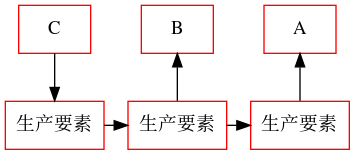
\includegraphics[scale=0.8]{weisebianji.png}
  \caption{\label{fig:weise}价值因果关系}
\end{figure}

边际效用经济学家认为,古典经济学家在声称价格取决于生产成本时是错误
的。\cref{fig:weise}揭示了这一所谓误解的准确性质。如果我们只考虑边际内产品,或者
肤浅地着眼于价格的形成,那么因果关系似乎就是从生产要素到价格——要素是决定价格的
因素。然而,根据边际效用经济学家的观点,仔细考虑这一过程就会发现,用来度量生产要
素价格的是生产要素在所生产的边际(或者说最后的最终产品,本例即胡萝卜(C))中产生的边际效
用。

\subsection{欧根·冯·庞巴维克}

庞巴维克与维色年龄相同;两人都是门格尔的学生,他们是朋友也是连襟。维色主要在奥地
利和德国有影响力,而庞巴维克在英国和美国更加为人所知。在庞巴维克的第一本书出版之
后,他在英国收了一个弟子,名叫威廉·斯马特(William Smart),他翻译了庞巴维克1890年
的《资本与利息》和1891年的《资本实证论》。门格尔在说英语的国家影响较小的一个原因
是,他的《原理》直到1950年才被翻译成英文出版。庞巴维克是一位造诣深厚的学者,他在
资本与利息领域的著作出版了三卷。第一卷《资本与利息:经济理论的批判史》涉及了远至
希腊的150多位经济学家。他花了大约二十年的时间来完成这套三卷本著作,在这期间的大部
分时间里,他是奥地利政府的重要人物。他对经济学的贡献,包括他对门格尔边际效用观点
的清晰说明与扩充,以及对资本与利息理论的发展(我们将在第9章中予以探讨)。像他的老师
门格尔以及他的同事和朋友维色一样,庞巴维克也没有运用数学。他运用推理的单因果关系
线条,详细说明关于价值或价格形成的观点,但他没有看出瓦尔拉斯和马歇尔所指出的相互
决定关系,这种关系现已成为现代经济思想的一个重要构件。

\subsection{走哪一条路——变化中的经济学范围与方法}

杰文斯、门格尔还有瓦尔拉斯,对现代经济学的技术工具做出了重大贡献,他们对于后来经
济思想的范围与方法也具有深远的影响。

三位经济学家都格外关注资源配置,或者被称作微观经济理论的东西。考虑到门格尔,我们
必须对这一宽泛的陈述进行限定,他在其《原理》第5部分考察了知识在人类福利进步中的作
用和影响。门格尔希望这样做能够补充和完善亚当·斯密对劳动分工的强调,即把劳动分工视
为国民福利提高的主要原因。不幸的是,门格尔的见解,即知识的作用是经济增长与发展的
因素,并没有被下一代的经济学家继续予以研究,他们变得几乎专门对资源配置感兴趣。
在1870--1900年期间,经济学从涉及斯密、李嘉图、穆勒的问题,转向研究价格系统如何运
行来分配稀缺资源。

尽管关于经济学的适当范围,杰文斯、门格尔、瓦尔拉斯之间具有几乎完全的一致性,然而,
关于适当的方法,他们的观点还是有分歧的。杰文斯追随威廉·配第的路线,提倡更多地运
用统计过程来确定经济变量之间的因果关系。门格尔偏重于更多地运用抽象推理,通过演绎
逻辑的使用构建学术模型。在这点上,他沿袭了李嘉图的方法。门格尔的研究缺乏数学、统
计学以及对历史过程或制度安排的论述。瓦尔拉斯的方法同样也缺少对时间或地点的抽象,
但是他确信,通过运用数学,能够了解市场经济的相关性和相互的因果关系。

经济学主流主要沿着两条道路前进:其一是更多地运用数学形式的抽象推理,即瓦尔拉斯所
建议的道路;另一个是更多地强调运用统计过程检验理论假设,即杰文斯所建议的道路。在
本书第四部分“现代经济学及其批判”中,我们将转向这类问题。

\subsection{杰文斯、门格尔以及瓦尔拉斯对后来经济学家的影响}

杰文斯从未有过追随者,所以,不存在杰文斯经济思想流派。马歇尔对英国经济思想的支配,
室息了杰文斯的贡献。杰文斯46岁时在一次游泳事故中过时离世,这也是他缺少追随者的原
因。瓦尔拉斯对边际分析的贡献,完全因其对一般均衡的阐述而失色。门格尔对经济学家和
经济学后来发展的影响,仍然在继续中。受到门格尔影响的相当多的经济学家在德国、英国
以及美国从事教学和研究;较早的一群人中包括米塞斯和熊彼特,较近的一群人中包括弗里
德里希·冯·哈耶克(1899--1992)、戈特弗里德·哈伯勒(1900--1995)以及奥斯卡·摩根斯
特恩(OskarMorgenstern,1902--1977)。在这些经济学家中,有些人独自研究,在任何重
要的方面都没有遵循奥地利传统,但有些人的确符合某种模式,我们能够描绘出从门格尔开
始,经维色、庞巴维克、米塞斯、哈耶克,到20世纪末奥地利经济学的世系。门格尔所提倡
的方法并没有为主流经济思想家所接受,他们更多地使用包含数学和统计学的方法。然而,
奥地利传统足以引起注意,所以,我们将在第13章中予以论述,并在第17章详细考察其现代
拥护者,那一章包含了一些现代非主流经济思想。

在受到门格尔影响的人中,很多都是市场驱动型经济体的拥护者,他们不满于社会主义者提
供的可替代选择。米塞斯和哈耶克在20世纪20年代开始的辩论中扮演了重要的角色,这些辩
论涉及:(1)社会主义经济体有效配置资源的能力,(2)资本主义、社会主义、经济与政治自
由三者之间的关系。我们在第13童中将转向这些问题,考察从事资本主义和社会主义研究的
奥地利经济学家及其他经济学家。

\section{总结}

凭借对边际分析的贡献,杰文斯、门格尔还有瓦尔拉斯,开创了新古典经济学。杰文斯和门
格尔认为,他们用需求导向的边际效用价值理论,替代供给导向的生产成本价值理论,对经
济理论进行着革命。然而,他们的希望没能得到实现,原因在于,他们专门强调需求方面,
同古典学者强调供给方面一样不完善。事实上,关于价值问题,杰文斯的和门格尔的看法从
根本上说是不合理的,因为他们在寻找边际效用与价格之间简单的因果关系。当古典经济学
家本质上假定需求既定,从而推断供给决定价格时,杰文斯和门格尔则假定供给既定,并推
断需求决定价格。瓦尔拉斯对价值问题有更加清晰的理解,因为他认识到经济体组成部分的
相互依赖。

三位经济学家对经济理论做出了五个永久性的贡献。(1)他们对边际效用和需求作用的强调,
促使后来的经济学家更多地注意价值理论中的这一部分内容。(2)他们对边际分析的运用,
导致人们对更普遍地使用这一方法的公认,这种公认对经济理论的发展产生了重要后果。
到1890年,边际分析已经被扩展到不仅涵盖家庭需求方面和厂商供给方面,而且包括厂商对
生产要素的需求方面。(3)杰文斯和瓦尔拉斯在经济理论化过程中对数学的应用,使经济学
家了解了这种分析类型的能力,并最终导致如今数学模型在经济思想中占支配地位。(4)就
提供市场经济不同部门相关性的见解,以及为后来的理论工作提供基础而言,瓦尔拉斯的一
般均衡模型是开创性的。(5)杰文斯对统计学的运用和认可,对于用计量经济学方法进行理论
检验的出现来说,泵重要的一步。

然而,边际分析的传播并不是迅速的,关于这一新方法,引起了很多和争议。我们将在接下
来的三章中研究边际主义和新古典微观经济学的成长。


%%% Local Variables:
%%% mode: latex
%%% TeX-master: "../../main"
%%% End:

\chapter{向新古典经济学的过渡:扩展的边际分析}

第一代边际理论家杰文斯、门格尔以及瓦尔拉斯,通过提出边际分析改变了经济学方
法。……更为显著的是,它结束了约翰·斯图亚特·穆勒的古典经济学。但是第一代理论家只
能部分地想象出这种工具的有用性。他们不能理解其发现的全部分量:相比古典学派,他们
强调\textbf{理论内容}方面的区别,远甚于强调\textbf{方法论}的区别。

因为早期边际主义者如此着力强调他们与李嘉图劳动价值理论结论的区别,所以他们未能认
识到自己与李嘉图构建的抽象模型之间的密切关系。\textbf{李嘉图在解释地租的决定力量
  时,也运用了边际分析。}通过运用数学工具,边际分析家们将边际主义逐渐应用于微观经
济学理论的各个部分。杰文斯和瓦尔拉斯两人都受过数学训练,但门格尔没有。第二代边际
理论家,除了门格尔的奥地利弟子之外,都运用微积分对经济理论的前沿问题进行研究。

由第一代边际理论家引起的潮流一直持续到现在。使用令人难忘的数学方法,发展高度抽象
的模型,这是今天的常态。这些发展受到一些人的地址,尤其是阿尔弗雷德·马歇尔、德国
与英国历史学派、美国制度主义者、新奥地利经济学家、激进经济学家,以及很多不被划分
为主流的经济学家。

\section{扩展的边际分析:第二代}

杰文斯、门格尔、瓦尔拉斯的理论内容在很多方面还有不完善之处。他们将边际分析几乎专
门用于需求理论,差不多完全忽视了供给理论。杰文斯和门格尔很少注意供给,原因是他们
为价值几乎唯一地取决于边际效用的观念所困扰。瓦尔拉斯也没有明显地专注于供给方面,
因为他在一般均衡模型集中于经济变量的相关性。

他们的模型绝大部分都假定供给是既定的,并且资源配置问题仅仅是在可替代的用途之间分
配固定供给的问题。更具体地说,他们没有解释当生产要素供给不固定时这些要素价格的决
定力量;没有解释收入分配的决定力量;没有对厂商经济学进行有意义的分析;没有洞察到
一些独特的问题,这些问题是在发展理论的过程中为了解释工资、地租、利润以及利息而必
须加以解决的。

实际上,边际分析已经被两位较早期的经济学家应用于要素定价和收入分配中,然而像戈森
一样,他们的成就在很大程度上被同时代的人忽视了。蒙迪福特·兰格菲尔德在《政治经济学
讲义》(1834)中批评了劳动价值理论,提出了一种边际生产力分配理论。但他并不为杰文
斯、门格尔、瓦尔拉斯以及马歇尔所知,他的著作1903年才通过E.R.A·塞利格曼的介绍而引
起经济学界人士的注意。尽管冯·杜能对微观经济学问题具有比较重要的见解,但是,阿尔弗
雷德·马歇尔似乎是早期唯一一个发现冯·杜能边际生产力巨大影响力的人。

实际上,\textbf{冯·杜能看来是将微积分应用于经济理论中的第一人。}他不仅能够形成不
同要素边际产品的概念,而且提出了一个基于这些原理的相当正确的分配理论。在冯·杜能用
了将近二十年的努力来应对“\textbf{所有的经济力量决定要素价格}”这一简单陈述所表达
的问题后,他非常满意自己的最终结果,所以,他要求在他的墓碑上刻上他关于劳动工资的
公式。但不幸的是,他的成就对后来的经济思想几乎没有直接的影响,虽然马歇尔大方地向
冯·杜能致谢。

第二代边际主义者凭借一种广泛应用于需求和供给理论的新工具,使经济理论得以复苏。然
而,这一工具几乎专门用来分析需求方面,尤其是家庭理论,很少用来分析供给理论或者厂
商理论。

来自奥地利、英国、瑞典以及美国的经济学家们,都对这一理论主体有显著的贡献,这不仅
表明这些成就代表了众多学者的共同努力,而且表明经济学作为一种学术上的努力,正变得
日益专业化。

\section{边际生产力理论}

收益递减原理在现代经济理论中发挥着根本性的作用。在微观经济理论中,它解释了厂商短
期供给曲线的形状,以及厂商的生产要素需求曲线形状。

李嘉图研究了今天所谓的农业生产函数,即土地的物质投入与物质产出之间的关系。他假定
生产过程中资本对劳动的比率因可利用的技术而固定,并且资本与劳动的组合以这种技术上
不变的比例添加到数量固定的土地上。在这些假设的基础上,他断定,对于连续的资本与劳
动组合来说,所形成的产量将呈现边际产品递减的特征。

经济分析史中的异常之一是,从李嘉图将边际生产力分析应用于地租的决定,到边际生产力
分析普遍应用于所有生产要素,花了将近七十五年的时间。一个类似的异常是,李嘉图所形
成的用于供给方面的边际分析,在19世纪70年代经历了首次重大扩展,当时,它不仅被用于
分析边际生产力,而且被用于分析边际效用。第二代边际主义者,最终挖掘出了为人所知的
收入的边际生产力理论的基础。这些经济学家中最重要的是奥地利学者弗里德里希·冯·维色
和欧根·冯·庞巴维克;美国学者约翰·贝茨·克拉克(John Bates Clark,1847--1938);瑞
典学者纳特·维克塞尔(Knut Wieksell,1851--1926);以及英国经济学家菲利普·亨利·维
克斯蒂德(Philip Henry Wicksteed,1844--1927)和弗朗西斯·Y·埃奇沃斯。这些经济学家,
连同杰文斯、门格尔、瓦尔拉斯以及马软尔,都是这一时期正统经济理论的智力伟人。他们
的首部重要著作都出现在1871年至1893年期间。

\subsection{收益递减原理}

如果保持一种生产要素不变,增加一种可变要素到这种不变要素上,因此形成的产量经常是
一开始增加速度递增,然后增加速度递减,最终递减。\cref{tab:productfunc}的例子显示了物质投入
与物质产出之间的这种关系。

% Please add the following required packages to your document preamble:
% \usepackage{booktabs}
% \usepackage{graphicx}
\begin{table}[htbp]
  \centering
  \caption{生产函数}
  \label{tab:productfunc}
  \small
  \begin{tabularx}{\linewidth}{@{}XXXX@{}}
    \toprule
    劳动 & 劳动的总产品\newline(谷物吨数) & 劳动的平均产品\newline(谷物吨数) & 劳动的边际产品\newline(谷物吨数) \\ \midrule
    0 & 0 & 0 & 0 \\
    1 & 10 & 10.0 & 10 \\
    2 & 21 & 10.5 & 11 \\
    3 & 33 & 11.0 & 12 \\
    4 & 46 & 11.5 & 13 \\
    5 & 58 & 11.6 & 12 \\
    6 & 68 & 11.3 & 10 \\
    7 & 75 & 10.7 &  7\\
    8 & 80 & 10.0 &  5\\
    9 & 83 &  9.2 &  3\\
    10 & 83 &  8.3 &  0\\
    11 & 80 &  7.3 &  -3\\ \bottomrule
  \end{tabularx}%
\end{table}

如果土地数量保持不变,例如为100英亩,每年使用1个人,那么将会发现总产品为10吨谷物。
然后用每年使用2个人来重复试验,记录一个21吨的谷物产量,等等。注
意,\cref{tab:productfunc}中劳动总产品一列的数据,被假定为在给定的不变投入和可变
投入数量下,能够被生产出的最大量的产品。简言之,它假定实现了最大化的技术效率。此
外,当记录这些“投入--产出”关系时,假定技术水平保持不变。

\begin{figure}[ht]
  \centering
  \begin{tikzpicture}[scale=0.8, baseline, remember picture]
    \datavisualization [school book axes,visualize as smooth line/.list={tpl,ap,mpl}
, style sheet=strong colors,
    % style sheet=vary dashing,
    % legend=north west inside,
    tpl={pin in data={text=$TP_L$, pos = 0.8}},
    y axis={length=5cm,ticks={step=10},label=总产品\phantom{/劳动}}, x axis={label=劳动,length = 8cm},
    ]
    data [set=tpl] {
      x, y
      0, 0
      1, 10
      2, 21
      3, 33
      4, 46
      5, 58
      6, 68
      7,75
      8,80
      9,83
      10,83
      11,80
    }

    info {
      \coordinate (blaL1) at (visualization cs: x=4, y=46);
      \coordinate (blaL2) at (visualization cs: x=5.25, y=61);
      \coordinate (blaL3) at (visualization cs: x=10, y=83);
    }
    ;
  \end{tikzpicture}

  \begin{tikzpicture}[scale=0.8,baseline,remember picture]
    \datavisualization [ school book axes, visualize as smooth line/.list={tpl,ap,mpl}, style sheet=strong colors,
    % style sheet=vary dashing,
    % legend=north west inside,
    ap={pin in data={text=$AP_L$, pos = 0.7}},
    mpl={pin in data={text=$MP_L$,  pos =0.75, }},
    y axis={label=总产品/劳动,length=5cm,ticks={step=2}}, x axis={label=劳动,length = 8cm},
    ]

    data [set=ap] {
      x, y
      0, 0
      1, 10
      2, 10.5
      3, 11
      4, 11.5
      5, 11.6
      6, 11.3
      7,10.7
      8,10.0
      9,9.2
      10,8.3
      11,7.3
    }

    data [set=mpl] {
      x, y
      0, 0
      1, 10
      2, 11
      3, 12
      4, 13
      5, 12
      6, 10
      7,7
      8,5
      9,3
      10,0
      11,-3
    }

    info {
      \coordinate (L10) at (visualization cs: x=4,y=0);
      \coordinate (L20) at (visualization cs: x=5.25,y=0);
      \coordinate (L30) at (visualization cs: x=10,y=0);
    }
    ;
  \end{tikzpicture}

  \begin{tikzpicture}[remember picture, overlay]
    \draw [blue,dashed,thick] (blaL1)  -- (L10)node [below = 12pt] {$L_1$} ;
    \draw[red,dashed,thick] (blaL2)  -- (L20) node [below = 12pt] {$L_2$};
    \draw [dashed,thick] (blaL3)  -- (L30) node [below = 12pt] {$L_3$};
  \end{tikzpicture}
  \caption{\label{fig:productfunc}劳动的总产品、平均产品、边际产品}
\end{figure}

\cref{tab:productfunc}从数字上显示了可变投入劳动的平均产品或边际产
品,\cref{fig:productfunc}从图形上将它们呈现出来。劳动的平均产品是用总产品除以劳
动数量计算出的。劳动的边际产品通常更为准确地被称作\textbf{劳动的边际物质产品},它
被定义为:
\[MPP_L=\frac{\Delta TP}{\Delta L}\]

在几何上,它是总产品曲线的斜率,或者说总产品对劳动的一阶导数。当劳动的数量
为$L_1$时,劳动的边际产品达到最大值,当劳动的数量为$L_2$ 时,劳动的平均产品达到最
大值,并且边际产品与平均产品\textbf{相等};当劳动的数量为$L_3$时,总产品达到最大
值,并且劳动的边际产品为零。劳动的数量超过$q_3$,将引起总产品下降,边际产品为负
数。

19世纪的最后几年间,生产函数的准确性质及其含义才慢慢挖掘出来,描绘并计算任何生产
要素的边际产品成为可能。例如,我们可以保持劳动数量固定,从而得出土地的边际产品曲
线。

\subsection{新的与旧的}

随着对生产中各种关系的更多理解,人们逐渐认识到,假定完全竞争行业中的某个厂商只使
用劳动这种可变的生产要素,生产要素的需求曲线能够从边际产品曲线中得出。厂商在完全
竞争的市场上销售其最终产品,因而最终产品的价格不随着厂商销售量而变化。换句话说,
厂商面对的是对其最终产品\textbf{完全有弹性}的需求曲线。厂商在\textbf{完全竞争}的
市场上购买可变投入;所以对厂商来说,投入的价格不随着购买的数量而改变。也就是说,
厂商面对的是对可变投入完全有弹性的供给曲线。\textbf{最理想的状态下,}厂商将把可变
投入固定到某一点上,在这一点上,\textbf{最后一单位所购买的投入为厂商的总收益所增
  加的数量,等于厂商的总成本所增加的数量。这个条件能被表述如下:}
\[劳动的价格=劳动的边际物质产品 \times 产出的价格\]

等式左侧度量的是由于另雇用了一单位劳动而增加的总成本。等式右侧度量的是由于销售劳
动所生产的产品而增加的总收益,它一般被称为边际产品价值。

考虑到\cref{tab:productfunc}中给出的数据,假定劳动的价格为每人每年10000美元,最终
产品的价格为每吨1000美元。如果本例中的厂商雇用5单位的劳动,那么,\textbf{最佳的劳
  动雇用等式}将会给出下列数值:
\begin{align*}
  P_L &=MPP_L \times P_o\\
  \$ 10000 &< 12 \times \$1000\\
  \$ 10000 &< \$ 12000
\end{align*}

所雇用的最后一单位劳动增加了10000美元的总成本和12000美元的总收益;因此,利润增加
了2000美元。\textbf{对利润最大化感兴趣的厂商,将增加对可变投入劳动的使用。随着这
  样做,劳动的边际物质产品下降。}所雇用的第六单位劳动增加了10000美元的总成本
和10000美元的总收益。第七单位劳动增加了10000美元的总成本,但只增加了7000美元的总
收益。最佳的劳动量是六单位,原因在于,劳动的价格等于劳动的边际产品价值。

然而,由于大多数生产过程涉及多种投入,所以,需要更一般化的投入品最佳使用原则。假
设我们有若干投入,$A, B, C , \cdots N$……当下列条件成立时,这些投入就以一种最佳
的方式被使用着:

\[\frac{MPP_A}{P_A} = \frac{MPP_B}{P_B} = \frac{MPP_C}{P_C} = \cdots = \frac{MPP_N}{P_N}\]

等式表明,当花在购买每种要素上的最后一美元产生了相等的边际物质产品时,投入就得到
了最佳使用。如果这一条件不能满足,就有可能改变要素购买,用相同的总成本生产更多的
最终产品,或者以较低的总成本生产既定的最终产品,这是同样的事情。

现在能够很容易得出对一种投入的需求。\textbf{对一种投入的需求被界定为厂商在不同价
  格下所雇用的数量。}假定我们从一家正最佳使用投入的厂商开始;也就是说边际物质产品
与投入价格的比率相等。如果我们降低一种投入的价格那么,厂商将会使用更多的这种投入,
直至花在这种投入上的最后一美元产生的边际物质产品,与花在所有其他投入上最后一美元
产生的边际物质产品相等。边际生产力理论也表明,当竞争性市场的厂商最佳地使用其投入
时,所有投入的价格都将等于其边际产品价值。

就像一些创始者所认同的那样,边际生产力的这些新观点与李嘉图的地租理论密切相联。分
析地租理论时,李嘉图假设资本与劳动就像是一种可变投入,按照由技术决定的固定比例,
运用到\textbf{土地这种不变投入}中,李嘉图借此\textbf{把一个三种投入的模型变为两种
  投入的模型}。为了说明最新发展的边际生产力理论与李嘉图地租理论之间的密切关系,我
们考虑只有劳动与土地两种投入的模型。在这一模型中,李嘉图按
照\cref{fig:richardoMP}所表示的方式度量了地租。

\begin{figure}[ht]
  \centering
  \subcaptionbox{\label{fig:richardoMPa}土地数量不变,劳动数量可变}{%
    \begin{tikzpicture}
      \draw (0,0) node[below left] {$O$};
      \draw[very thick] (0,5) -- node[left=12pt, text width =1em] {劳动的边际产品} ++(0,-5)  -- node[below=10pt] {劳动} ++ (6,0);

      \coordinate (a) at (0,4);
      \coordinate (m) at (4,1);
      \coordinate (b) at ($(a)!0.6!(m)$);
      \coordinate (d) at ($(a)!(b)!(0,0)$);
      \coordinate (c) at ($(0,0)!(b)!(6,0)$);

      \draw (a) node [left] {$A$} -- (m) node [below right] {$M$};
      \draw[dashed] (b) node [right] {$B$} -- (d) node [left] {$D$} node[pos=0.6, above = 0.1cm] {地租};
      \draw[dashed] (b) -- (c) node [below] {$C$} node [pos=0.5, left=18pt] {工资};
    \end{tikzpicture}%
  }\hfill
  \subcaptionbox{\label{fig:richardoMPb}劳动数量不变,土地数量可变}{%
    \begin{tikzpicture}
      \draw (0,0) node[below left] {$O$};
      \draw[very thick] (0,5) -- node[left=12pt, text width =1em] {土地的边际产品} ++(0,-5)  -- node[below=10pt] {土地} ++ (6,0);

      \coordinate (a) at (0,4);
      \coordinate (m) at (4,1);
      \coordinate (b) at ($(a)!0.6!(m)$);
      \coordinate (d) at ($(a)!(b)!(0,0)$);
      \coordinate (c) at ($(0,0)!(b)!(6,0)$);

      \draw (a) node [left] {$F$} -- (m) node [below right] {$N$};
      \draw[dashed] (b) node [right] {$G$} -- (d) node [left] {$I$} node[pos=0.6, above = 0.1cm] {工资};
      \draw[dashed] (b) -- (c) node [below] {$H$} node [pos=0.5, left=18pt] {地租};

    \end{tikzpicture}%
  }
  \caption{\label{fig:richardoMP}李嘉图地租理论的劳动与土地边际生产力模型}
\end{figure}


在\cref{fig:richardoMPa}中,曲线 $ABM$ 表示劳动的边际物质产品。如果使用等
于 $OC$的劳动数量,那么,总产品就是面积$OABC$即边际产品的总和。然而,李嘉图并不集中
于边际产品,虽然他假设边际产品递减。他集中研究地租的决定。他推断地租等于面积$ABD$。
每个劳动者得到的工资为$OD=BC$,总工资支出为面积$ODBC$。从总产品中减去总工资就得到剩余
的$ABD$,它就成了不变生产要素土地的地租。

在\cref{fig:richardoMPb}中,曲线$FGN$度量了土地的边际物质产品。总产品等于面
积$OFGH$,每一单位土地获得的地租为$OI=HG$,总地租为$OIGH$。现在,工资就用不变要素
劳动的剩余增加量来度量,它等于$FGI$。

因此,新的边际生产力理论的一个结果,就是适应了李嘉图的地租理论并使之一般化。李嘉
图所强调的\textbf{不是可变投入的边际产品},而是\textbf{不变要素的剩余增加量}。然
而,新的理论集中于\textbf{可变投入的边际产品}。李嘉图内将边际生产力分析应用于地租
的决定,而新的理论家认识到\textbf{任何一种投入都能够改变},并且它们的边际产品能够
被计算出来。他们也看到,厂商将继续投入,直至投入的价格等于可变投入的边际产品价值。
这些新的观点引发了这一时期广为争论的很多问题。

\subsection{产品用尽}

李嘉图的分配理论在下列意义上来说是一种\textbf{剩余理论},即地租是将工资和利润从总
产品中扣除之后的剩余;利润是将工资(马尔萨斯人口学说所定义的工资)从工资与利润
(李嘉图分配理论中的工资与利润)之和中扣除之后的剩余(见第5章7.1小节“分配理
论”)。根据剩余分配理论,支付给不同生产要素的报酬等于总产品,这一点不存在问题,
因为决定要素报酬的方法保证了总产品被予以分配。

我们假定一个只有劳动与土地两种投人的简单经济体。利用李嘉图剩余理论来解释收入的分
配,我们的推理如下:\cref{fig:richardoMPa}表明经济体的总产品等于 $OABC$,劳动获得
的份额等于 $ODBC$,剩余的就是地租或者说总产品与总工资支付的差额。因为地租是作为一
种剩余计算出来的,所以,工资加上地租一定等于总产品。然而,边际生产力分配理论并不
能这么明显地得出这一结论。如果在竞争性市场上,每种要素获得其边际产品价值,那么,
有理由假定\textbf{所有这些边际产品的总和将恰好等于总产品吗}?

新近发展的边际生产力理论主张,每种要素将获得其边际产品。通
过\cref{fig:richardoMPa},我们断定劳动的边际物质产品为$BC$,总工资支出等于所使用
的劳动数量 $OC$乘以劳动的边际产品,从而得到面
积 $ODBC$。在\cref{fig:richardoMPb}中,土地的边际物质产品为 $GH$,总地租为土地的
边际产品 $GH$ 乘以土地的数量 $OH$即面积 $OIGH$。如果两者都用边际产品方法来计算,
那么工资与地租的总和等于总产品吗?面积 $ODBC$(工资)加上面积 $OIGH$(地租)等于
面积 $OABC$(总产品)吗?换句话说,用边际产品方法计算的工资 $ODBC$ 等于用剩余方法
计算的工资 $IFG$ 吗?同样的问题也可以用于地租:$OIGH$等于 $DAB$ 吗?支付给生产要
素的报酬等于总产品的主张,可以用下面的等式形式来表达:
\[Q=MPP_L·L + MPP_T · T\]

这里的 $Q$为产出的物质数量(总产品),$MPP_L与MPP_T$为劳动与土地的边际物质产
品,$L与T$是劳动与土地的数量。

约翰·贝茨·克拉克声称,\textbf{支付每种生产要素其边际产品,将正好用尽总产品},但是,
他没有为这一主张提供证据。19世纪90年代展开了对这个问题的争论,并一直持续到20世纪。
其中所涉及的最重要的经济学家有威克斯蒂德、维克塞尔、巴罗内(Barone)、埃奇沃斯、
维尔弗雷多·帕累托(Vilfredo Pareto,1848--1923)以及瓦尔拉斯。\footnote{对这个问
  题公认的最好总结,包含在乔治·斯蒂格勒的《生产与分配理论》第12章“欧拉定理与边际
  生产力理论”中。该书由美国麦克米兰出版公司于1941年出版。}我们将集中评论威克斯蒂
德和维克塞尔,他们的贡献极大地影响了边际生产力理论的发展。

1894年\textbf{P. H·威克斯蒂德}出版了一本题为《论分配法则之协调》的小册子,他在其中
提出,古典理论要求\textbf{分别解释}支付给土地、劳动、资本的报酬,在这点此是不完善
的,而边际生产力理论用一个\textbf{统一的原理}来解释任何生产要素的收益,从这点上说
它是一种更好的理论。维克斯蒂德断定在竞争性市场上,每种生产要素将拥有等于其边际产
品价值的一个价格——他承认,这就提出了\textbf{如果所有的要素获得其边际产品、总产品
  是否被用尽}的问题。他试图证明这一结果,即所说的产品用尽将会发生。尽管他在这一尝
试上未能成功。然而威克斯蒂德的确指出,发生产品用尽\textbf{必须存在竞争},并且,厂
商的生产函数必须具有某些性质。在对威克斯蒂德《论分配法则之协调》的评论中,A. W·弗
拉克斯(A. W. Flux)也对这些发展有所贡献。他证明只有当生产函数具有某些数学性质时,
才会导致产品用尽。瑞士一位数学家莱昂哈德·欧拉早先考察过这些性质,他的名字因此开始
与涉及产品用尽的问题相关。

对于因支付给每种要素的报酬等于其边际产品,而使总产品恰好用尽来说,\textbf{生产函
  数必须具有如下性质,即所有投入增加既定的比例将使产量或总产品按相同的比例增加。}在
我们的例子中,如果劳动与土地的数量增加一倍,那么,总产量增加一倍;如果两种投入增
加两倍,那么,总产量增加两倍,等等。适用于这些函数的数学习语是,它们是\textbf{一
  次齐次}(homogeneous to the degree one)的。这些函数也被描述为“\textbf{线性齐
  次的}”,尽管这样一种描述可能会误导不是数学家的人,因为它们不一定是线性的。小于
一次齐次的生产函数会引起一种状况,即所有投入增加一定比例,引起产量以较低的比例增
加。如果生产函数是大于一次齐次的生产函数,那么所有投入增加一定的比例,将引起产量
以较高的比例增加。

经济学家使用\textbf{规模收益}这一习语来描述产量或成本对所有投入成比例增加的反应方
式。如果所有投入都成比例增加,并且总产量也增加了相同的比例,那么,平均成本不变,
这种结果被称为规模收益不变。规模收益不变由一次齐次生产函数得出。如果所有投入都成
比例增加,并且总产量增加了一个较小的比例,就存在规模收益递减,平均成本增加。规模
收益递减由小于一次齐次的生产函数得出。

在\textbf{完全竞争市场上}销售其产出并购买其投入的厂商,如果拥有能够产生规模收益不变的生产
函数,将会发现,如果所有的投入按照其边际产品价值来支付,那么,厂商的总收益将完全
被这些支付用尽。要素市场上的竞争将导致每种投入获得其边际产品价值,最终产品市场上
的竞争,其结果是厂商获得零利润。如果获得零利润,那么,厂商的总收益必定等于总成本;
因为总成本是给各种投入的支付,所以,就发生了产品用尽。

一个简单的代数表达式能阐明这个问题。所陈述并在这一时期被讨论的问题是,为每种投入
支付其边际产品是否用尽了厂商的总产品。对于一个简单的劳动与土地生产函数,我们先前
用等式的形式来表述这个问题:

\begin{align*}
  Q &=MPP_L \cdot L + MPP_T \cdot T
  \shortintertext{乘以最终产品的价格后}
  PQ &= P \cdot MPP_L \cdot L +P \cdot MPP_T \cdot T
  \shortintertext{现在} P \cdot MPP_L &= 劳动的边际产品价值(VMP_L)
  \shortintertext{并且} P \cdot MPP_T &= 土地的边际产品价值(VMP_T)
  \shortintertext{因此}
  PQ &= VMP_L \cdot L + VMP_T \cdot T
\end{align*}

等式右侧表示支付给劳动的总报酬与支付给土地的总报酬。因此,它代表了厂商的总成本。
等式左侧表示厂商的总收益。在完全竞争下,所有投入获得其边际产品价值,并且利润为零,
这意味着厂商的总收益将等于总成本。于是,支付给生产要素的报酬用尽了厂商的总收益。

\textbf{大于一次的齐次生产函数引起规模收益递增和平均成本下降。这意味着边际成本一
  定低于平均成本,且一种投入的边际物质产品将超过此种投入的平均产品。}如果投入是在
竞争性市场上购买的,那么,厂商必定要为每种投入支付其边际产品价值。但
是,\textbf{如果所有的投入获得其边际产品价值,那么,厂商的总收益将会低于支付给所
  有投入的报酬。}从成本或者从产出的角度处理这个问题,都能证明这一结果。如果经历平
均成本递减的厂商,其行为是竞争性的,即在等于边际成本的价格上销售其产品,那么,这
种操作是亏本的;也就是说,总成本将会超过总收益。类似地,如果投入的边际物质产品超
过了其平均产品,并且投入获得等于其边际产品的报酬,那么,支付给投入的报酬将超过总
产量,厂商将\textbf{亏损}。

\textbf{小于一次的齐次生产函数引起规模收益递减或者平均成本递增,在此,边际成本高
  于平均成本,一种投入的边际物质产品将低于此种投入的平均产品。}具有竞争性行为的厂
商,将使边际成本等于价格,在那一产量上将会获得利润。这就暗示了,当所有要素获得其
边际产品价值时,支付给投入的报酬将少于总产量。在这些情况下,总收益超过总成本,厂
商将获得\textbf{利润}。

\subsection{维克赛尔论产品用尽}

\textbf{纳特·维克塞尔}是一位瑞典经济学家,为宏观与微观经济理论做出了很多重要的贡
献,他也是边际生产力理论的早期独立发现者。他对于欧拉定理和产品用尽相关的问题感兴
趣,与他所处时代的任何其他经济学家相比,维克塞尔为解决这些问题做出了更大的贡献。
在他关于这一主题的较早作品中,像大多数其他经济学家一样,他认为一个既定厂商或行业
将呈现规模收益递增、不变或者递减。这些类型似乎是相互排斥的。然而,1902年,维克塞
尔得出了一个完全不同的结论,即\textbf{既定厂商可能会经历规模收益的所有三个阶段}。

正在扩大产量的厂商将首先经历规模收益递增,但迟早会遭遇规模收益递减。在收益从递增
变为递减的产量水平上,一定会发生规模收益不变。维克塞尔明确地形成了厂商长
期\textbf{U形平均成本曲线}的概念,这一概念表明平均成本递减,然后达到一个最低点,
最后递增。维克塞尔认为,厂商的生产函数不一定是一次齐次的,从而发生产品用尽。如果
厂商在长期平均成本曲线的最低点所出现的产量水平上生产,并且利润为零,那么,会发生
产品用尽。维克塞尔推论完全竞争的市场将会导致这些结果,原因在于竞争将引起每个厂商
在最小成本下生产,并使利润为零。这样,尽管厂商的生产函数会形成收益递增、不变以及
递减,然而,竞争将会保证在长期均衡状态下,厂商在其生产函数的某一点上运转,在这一
点上,存在收益不变;在这一点上,函数是一次齐次的;在这一点上,平均成本是最小的。

维克塞尔在关于产品用尽问题的解决方案中,提出了新的引起注意的理论问题,经济学家们
始终追踪着这些问题,直至20世纪。维克塞尔提出了对长期平均成本曲线形状的一些解释,
但是,在20世纪30年代之前,这些问题一直没有被彻底弄明白。

\subsection{边际生产力理论的道德含义}

\textbf{约翰·贝茨·克拉克}独立发现并发展了\textbf{边际效用与边际生产力}观点。他对
边际效用理论的发展不如杰文斯、瓦尔拉斯或门格尔那样敏锐,但是,他对收入的边际生产
力理论的贡献,等同于第二代英国和欧洲经济学家。克拉克承认,他对边际生产力理论的发
展,是对美国社会评论家亨利·乔治所提出问题的回应。我们在第5章中了解到,享利·乔治断
定,土地的收益是一种不劳而获的收入,因此他质疑地租的合理性。乔治的主张促使克拉克
试图确定由个别生产要素产生的产品,以及边际生产力理论。约翰·贝茨·克拉克的儿
子J. M·克拉克也是一位重要的经济学家。

他的《财富的分配》包含了其边际生产力分配理论的实质,也包含了对竞争性市场所产生的
合意的道德后果的广泛发展。没有必要详细地展开克拉克对\textbf{边际生产力理论}的贡献。
有关的要点是他的以下结论,即\textbf{在完全竞争市场中,每种生产要素将获得等于其边
  际产品价值的收益。}这一收益度量了一种要素对正在生产的特定产品的贡献,也度量了它
对社会的贡献。资本的收益通过\textbf{资本是生产性}的这一事实被证明是正当
的;\textbf{收益不是抢夺,而是诚实、公平以及公正的。}同样,土地的收益也不是一种不
劳而获的收入,而是土地生产力的收益。同样的结论也适用于劳动的收益。克拉克的结论是,
完全竞争市场所产生的收入分配,是一种道德上正确的分配,因为它根据生产要素对社会产
品的经济贡献,对它们进行了奖赏。他主张,\textbf{剥削理论和不劳而获收入理论是天真
  的,}原因在于,它们未能了解经济体中\textbf{市场力量的运作}。

约翰·贝茨·克拉克对边际分析,尤其是对边际生产力理论的贡献,为他获得了全世界的认可。
他是第一位对经济理论做出重要贡献的美国经济学家,这样认为是公平的。然
而,\textbf{他从边际生产力理论中得出的道德结论},与他对实证理论的贡献相比,吸引了
更多的批判性注意。这么认为或许更公平些,因为克拉克把他的道德结论视为他最重要的贡
献。

他的主张即竞争性市场导致道德上合意的收入分配到底具有多少价值呢?这一主张最重要的
问题是它违背了\textbf{休谟格言:它从非道德的分析中得出道德含义。一个人“应当”获
  得的,可能与他或她真正获得的没有什么联系。}很多其他的问题也被提了出来。例如,即
使给定完全竞争市场的假设,也没有理由断定因为每种要素(factor)获得其边际产品价值,
所以每个个体(individual)就获得了一种收益,这种收益度量了他或她对经济体和社会的
贡献。个体的收入将取决于他或她在市场上销售的要素的价格,以及所销售的要素的数量。
拥有资本和土地的个体将获得这些来源的收入,但是,这些报酬代表了要素的贡献,而不是
个体的贡献。

克拉克道德结论的另一个难题是他对完全竞争市场的依赖。克拉克明白\textbf{厂商与工会
  两者的垄断力量},并试图将垄断力量的影响置于收入分配和他的道德结论中。
他\textbf{特别乐观}的观点使他将这些与竞争性市场的背离视为\textbf{在数量上无关紧
  要}。有趣的是,他最有才华的学生之一托尔斯坦·凡勃仑也观察了的同样的经济体与社会,
并且就它们的道德结果来说,得出了完全不同的结论。

\subsection{作为一种就业理论的边际生产力理论}

尽管边际生产力分析在最初形成时,是为了解释生产要素的价格决定力量与收入分配,但是,
人们很快就认为,它也能被用来解释就业水平的决定力量。在一个局部均衡分析的框架中,
如果劳动的价格上升,厂商将雇用较少的劳动,直至劳动的边际产品价值等于较高的劳动价
格。雇用较少的劳动会引起劳动的边际物质产品增加,因此提高劳动的边际产品价值。在行
业水平上,劳动的价格取决于对劳动的需求和劳动的供给,对劳动的需求又得自于劳动的边
际产品价值。如果一个行业中,劳动的价格在均衡水平之上,那么,所供给的劳动数量将超
过所需求的劳动数量——存在劳动的过剩或者说失业。

当边际生产力分析家将这一理论扩展到整个经济体时,他们断定,超过摩擦性失业的失业是
由于盛行的工资高于均衡水平而导致的。劳动的超额供给,就像任何其他商品一样,是通过
供求分析得到解释的。考虑到这种分析和有弹性的工资率,市场系统会自动纠正失业,因为
工资会下降。失业是劳动市场非均衡的体现;当劳动市场恢复均衡时,失业就会消除。以边
际生产力的这一应用为基础,人们在不同时期得出了很多政策结论:工资应当保持弹性,任
何对弹性工资的妨碍,例如,工会合约或最低工资法,都是不合意的;工会与最低工资法会
导致失业;如果经济萧条产生了失业,那么,使工资表失弹性的制度因素,将阻止市场通过
降低工资而自动消除失业。

\textbf{从边际生产力理论中得出的宏观经济政策结论是,通过允许工资下降,能够消除经
  济萧条与失业。}尽管一些经济学家基于社会理由,很不情愿地提倡降低工资来消除失业和
治理经济萧条,然而,正统理论得出这些结论是没有什么疑问的。在讨论这个问题时,阿尔
文·汉森(Alvin Hansen,1887--1975)引用了亚瑟·C·庇古20世纪20年代的著作,这些著作
描述了就业与工资之间的这样一种关系。汉森说,他提名“庇古是20世纪经济学家普遍接受
的思想中最杰出的(此外,也是最有社会头脑的)代表;很多经济学家无数次地提到他(也
包括我自己较早著作中的段落),任何人都能容易地增加关于他的内容,只要不怕麻烦这样
做”。这些观点都是从边际生产力理论中产生的,在20世纪30年代中期,在受到约翰·梅纳
德·凯恩斯严厉批评之前,这些观点一直为正统理论家所主张。诺贝尔奖获得者经济学
家\textbf{约翰·R·希克斯}(John R. Hicks,1904--1989)在他的《工资理论》(Theory
of Wages,1932)中,拿出两章来论述工资规制与失业。希克斯断定,\textbf{由于工会的
  压力或者由于立法而人为地使工资高于竞争性均衡的工资,将导致失业,}并且“失业必定
会持续,\textbf{直到人为确定的工资被放松,或者直到竞争性工资上升到人为确定的水
  平}”。

\begin{figure}[ht]
  \centering
  \begin{tikzpicture}
    \draw (0,0) node[below left] {$O$};
    \draw[very thick] (0,5) node[above] {价格} -- (0,0)  --  (6,0) node[right] {数量};

    \coordinate (d) at (0.75,4);
    \coordinate (d1) at (4,0.8);
    \draw (d) node [above left] { $D$} -- (d1) node[below right] { $D'$};

    \coordinate (s) at (4,4);
    \coordinate (s1) at (0.75,0.8);
    \draw (s) node [above right] { $S$} -- (s1) node[below left] { $S'$};

    \coordinate (X) at (intersection cs:first line={(d)--(d1)}, second line={(s)--(s1)});
    \draw [dashed] (X) -- (X -| 0,3) node [left] (we) {$W_e$};

    \coordinate (b) at ($(s)!0.2!(s1)$);
    \draw [dashed] (b) -- (b -| 0,3) node [left] (w1) {$W_1$};
    \draw [dashed] (b) -- (b |- 3,0) node [below] (q2) {$Q_2$};

    \coordinate (a) at (intersection cs:first line={(b)--(w1)}, second line={(d)--(d1)});
    \draw [dashed] (a) -- (a |- 3,0) node [below] (q1) {$Q_1$};

    \draw[ultra thick,decorate,decoration={brace,mirror},red] (q1.south)-- node[below] {失业} (q2.south) ;

  \end{tikzpicture}%
  \caption{\label{fig:mshiye}非均衡的劳动市场}
\end{figure}

我们能用\cref{fig:mshiye}中的简单供求分析来阐明这一推理。劳动的需求曲线 $DD'$ 为
劳动的边际产品价值。在工资上,被雇用的劳动数量为 $OQ_1$,。厂商将雇用劳动,一直到
所支付的工资等于劳动的边际产品价值的那一点上。在工资 $W_1$上,所提供的劳动数量
为 $OQ_2$ 。在工资 $W_1$上,劳动的超额供给等于 $Q_1Q_2$,它被称作失业。如果市场自
由运行,工资将下降到均衡水平 $W_e$上,失业将消失。因此,\textbf{失业是(1)劳动市
  场暂时非均衡的结果,或者(2)阻止工资下降的某些障碍的结果。}

边际生产力理论加上其\textbf{强烈的自由放任市场导向},使得美国的经济学家们
在20世纪30年代早期提出,减轻经济萧条的最佳政策是使政府置身于经济体之外,让市场运
行,从而降低工资。我们来简要地考察一下凯恩斯对把边际生产力理论作为一种就业理论的
主要批评。边际生产力理论声称,在竞争性市场上,工资将等于劳动的边际产品价值。劳动
的边际产品价值是劳动的边际物质产品乘以最终产品的价格。\textbf{凯恩斯指出,从厂商
  的观点来看,工资是一种成本,而从工人的角度来看,工资是收入。}因此,工资率的削减,
降低了厂商的成本,也降低了劳动者的收入。\textbf{当劳动收入开始下降时,最终产品的
  需求及其价格也将下降。最终产品价格的下降将引起劳动的边际产品价值下降。边际生产
  力理论作为一种就业理论的难点在于,它假定降低工资不会减少对最终产品的需求一一换
  句话说,总供给与总需求并不是互相连接的。}理论只集中于工资削减的成本方面,忽视了
凯恩斯所说的\textbf{总需求}。

\subsection{受到批判的边际生产力理论}

对边际生产力的批评一直持续到现在。早期的批评包括对边际生产力一般理论的广泛抨击,
无论理论是应用于劳动、资本还是土地;批评也包括对特殊问题的具体论述,这些特殊问题
起因于将理论应用于利润与利息的决定时。下一部分我们将讨论这些特殊问题,现在,着眼
于对边际生产力理论最重要的早期批评,即度量一种生产要素的边际产品是不可能的。

评论家表示,厂商、行业或经济体的最终产量是劳动、土地、资本联合努力的结
果,\textbf{不可能区分起作用的要素的边际产品}。F. W·陶西格
(F. W. Taussig,1859--1940)在哈佛大学经济学系的早期发展中是一位发号施令式的人物,
他在其有影响力的《经济学原理》中声称,在使用资本与劳动的过程中,“工具在一方,使
用工具的劳动者在另一方,不存在这样的分离。……我们无法明确分离劳动的产品与资本的
产品。”这一批评更大众化的说法包含在\textbf{乔治·伯纳德·肖}(George Bernard Shaw)
令人愉快的《聪明女人的社会主义和资本主义指南》中。肖认为,尽管通过给予每个人所生
产的产品来奖赏劳动,可能是合意的,然而,这是做不到的:“当一个农场主与他的劳动者
播种并收割了一块麦地时,世上没有人能说清他们中的每个人种了多少小麦。”又如,假定
木匠(劳动)使用铁锤(资本)在盖一座房子。如果增加另一单位的木匠,其边际物质产品
是什么?\textbf{在任何生产过程中,增加劳动通常都要求同时增加资本,这样就产生了区
  分新增劳动的边际产品与新增资本的边际产品的困难。}\textbf{马歇尔}就这个问题的解
决方案是,通过从新增劳动与资本的边际产品价值中\textbf{扣除资本成本来度量劳动的净
  产品}。\textbf{约翰·贝茨·克拉克}提供了另一种方案,他提出\textbf{资本的数量保持
  不变,但是其形式可以改变。}然而,因为资本的形式只能随着时间而改变,所以,克拉克
的方案就功际产品的计算问题提出了一种长期观点。

\section{利润与利息}

边际生产力理论的一些早期发展者,尤其是庞巴维克觉察到,尽管边际生产力分析对于劳动
和土地收益来说,是一种令人满意的解释,但是,它未能解释为人所知的利润与利息收益问
题。回顾以往,我们能看到,与解释利润与利息性质和数量相关的问题,在边际生产力分析
形成之前,其至没有出现过。

古典经济理论通常将生产要素划分为劳动、土地、资本。劳动的收益是工资;土地的收益是
地租;资本的收益是利润。利润这一术语,就像古典经济学家所使用的那样,包括了今天所
谓的利润与利息。未能区分利润收益与利息收益是可以理解的,原因是当时的典型厂商结合
了资本家与企业家的角色。投资基金的供给者与管理者是同样的一个人,所以,没有对利润
与利息进行区分。在我们所研究的这一时期,一项成就是认识到需要对这两者进行区分。

我们利用边际生产力理论,不仅能够解释劳动的工资、土地的地租、资本的利息,而且能够
解释流向企业家的利润吗?当时的经济学家断定,边际生产力理论能够令人满意地解释工资
与地租,然而利润与利息所特有的问题则要求更加成熟的理论予以解释。

\subsection{利润理论}

尽管\textbf{古典经济学家不加区别地将利润这一术语用于指资本家——企业家的全部收入},
然而,他们的确也意识到这种收入至少包含三种不同因素的报酬:\textbf{对使用资本的报
  酬,给予企业家所贡献的管理服务的报酬,以及补偿经济活动风险的报酬。}支付给厂商的
对使用资本的报酬(假定这一报酬不涉及风险)被归入\textbf{利息}(interest)的现代分
类中,我们将在紧接着的那部分进行讨论。\textbf{我们能将企业家才能确定为第四种生产
  要素,}从而将企业家的边际产品界定为他对厂商的管理服务贡献与风险承担贡献的度
量\textbf{吗}?

\textbf{约翰·贝茨·克拉克}是边际生产力理论最重要的早期发展者,他认识到这种解决方案
并不令人满意。\textbf{企业家作为管理者的收益并不是利润,而是工资。}利润——或者更加
准确地说纯利润——一定被界定为,在厂商使用的全部投人被支付了等于其机会成本的价格之
后残留的剩余。长期均衡下的完全竞争市场,使所有要素获得其边际产品价值,亦即其机会
成本。假定在一个齐次生产函数中,这些支付就是厂商的成本,当从总收益中减去时,会产
生一个零利润率。因此,\textbf{利润的存在一定被解释为,或者是竞争性市场没有达到长
  期均衡,或者实际市场不是完全竞争市场的结果。}

当然,长期竞争性均衡是一种理论上的构造,\textbf{没有市场符合这一构造。}然而,当我
们分析出现在非长期均衡的市场或经济体中的利润时,\textbf{还是保留竞争性的假设。}当
厂商购买投入、生产某种产出时,他们承担着风险。必须估计产量的最终价格,并且,投入
的价格以及支付给投入的报酬成了契约债务。如果厂商的总收入超过支付给投入的报酬就产
生了利润;如果收入小于支付的报酬就产生了亏损。于是,完全竞争市场中的利润可以被解
释为当经济体向长期均衡的新位置移动时所出现的非均衡结果。

\textbf{克拉克、马歇尔、熊彼特提出,应将利润解释为由经济体动态变化所产生的暂时性
  收入。}假定经济体处于长期均衡中,所有要素获得等于其机会成本的收益,并且,一个典
型厂商的收入等于其成本。消费者偏好的变化或者某种技术变革将为一些行业带来利润。然
而,随着资本向那些超过正常收益率的市场转移,通过竞争性力量,这些利润将会被消除。
因此,\textbf{利润不是生产要素的收益,而是与经济体中的动态因素相连的意外好运。}

\textbf{弗兰克·H·奈特(Frank H. Knight,1885--1972)通过将风险要素、管理能力、经济
  变革结合成一种理论,颇有意义地使先前的利润理论成为一体并加以扩展。}在《风险、不
确定性与利润》中,奈特区分了厂商所采取的能够投保的风险和没有有效保险的风险。例如,
一个厂商可能会在火灾中失去其设备,但精算知识允许运用保险来弥补这一风
险。\textbf{保险费用成了厂商成本的一部分。因此,这种风险并不是利润的来源。利润之
  所以存在,是因为市场中存在不适合保险的不确定性。这些都起因于市场的动态变化。}然
而,如果我们\textbf{放弃完全竞争的候设},利润则可能由于很多原因而出现,最重要的
是\textbf{垄断与买主垄断}。资本与利息理沦随着边际生产力理论的发展,经济学家开始更
加细致地区分利润与利息。这使得普遍公认的利润理论得到发展,然而,资本与利息理论直
到今天还存在争议。\textbf{罗伯特·M·索洛(Robert M. Solow)写道:“当一个理论问
  题80年后还保留着争议时,就存在一种推测,即这一问题是以不适当的方式引起的——或者
  的确非常深奥。”}C. E·费格森(C. E. Ferguson)就资本理论尚未被解决这一特征,提出了
若干理由:
\begin{quotation}
  每个人都知道,或者明显地觉察到资本理论是不容易的。对于这一点,存在一个肤浅的理
  由,即大量资本理论的文献陷入了辩论术和语义学中。但是,也有一个更为本质的原因。
  资本理论必然要涉及时间;而时间又涉及预期和不确定性,虽然我们一般通过假定一种静
  止状态,或者一条黄金时代的增长路径将它们去除。
\end{quotation}

我们将首先通盘考虑自1890年以来资本与利息理论的发展。包括熊彼特、费雪还有奈特在内
的一组经济学家,对资本的性质和利息存在的原因进行了广泛的哲学研究。另一组经济学家
只是在表面上略微谈到利息存在的原因,而集中解释决定利息率的经济力量。利息率决定力
量的理论可以被划分为非货币的、货币的以及新凯恩斯的,最后一种是最早由希克斯提出的
模型中另外两种方法的综合。非货币利息理论集中研究决定利息率的长期实际力量,因此属
于古典传统,这些理论从重商主义后期一直持续到20世纪30年代。货币利息率理论包括可贷
资金理论与流动性偏好理论。从1890年至20世纪30年代,利息理论方面三位最重要的经济学
家是庞巴维克、奈特和费雪,我们在本章考察他们的理论。

\textbf{重商主义者强调经济体中货币的作用,以及因此形成的货币利息理论。}他们主张,
货币数量的增加不仅提高了价格总水平,降低了货币价值,而且降低了利息率的一般水平。
在重商主义阶段的稍后时期研究利息理论的一些经济学家进行了更加敏锐的分析。尽管理查
德·坎蒂隆提出了一种非货币利息理论,然而,他也指出货币数量的增加能够引起利息率的上
升或者下降。如果货币供给的增加首先到了节俭的人手中,利息率将下降。但是,如果货币
首先到了挥金如土的人手中,利息率将会上升,原因在于,支出的增加将引起厂商投资增加,
从而使可借贷资金的需求增加。

古典理论聚焦于国民财富的长期实际决定力量,发展出非货币利息或者说实际利息理
论。\textbf{古典经济学家认为,利息率取决于投资支出的收益率。货币力量在短期内能够
  改变利息率,但是在长期中,决定利息率的是资本生产力这种实际力量。}李嘉图最为简洁
地表达了这一观点,他说:
\begin{quotation}
  利息率取决于由于使用资本所能获得的利润率,并且完全与货币的数量或者货币的价值无
  关。无论银行是贷出一百万、一千万还是一亿,都不会永久地改变市场利息率,只能改变
  它们所发行的货币的价值。
\end{quotation}

我们能引用\textbf{李嘉图}的其他段落来表明,他的确意识到\textbf{利息率并不是与货币
  数量“完全无关”}的。核心问题是,古典经济学家对经济体中\textbf{长期力量}的关注
导致他们不强调货币力量,其原因在于,货币力量只对利息率有短期影响,并不能改变资本
的生产力,资本的生产力才是长期中决定利息率的实际力量。宽泛地来看,
从1500年至1750年大约250年的时间里,时兴货币利息理论;从1750年至1930年大约180年的
时间里,正统理论家提出了非货币利息理论。20世纪30年代期间,出现了两种新的货币利息
理论,即流动性偏好理论与可借贷资金理论,随着这两种理论的出现,人们认识到一般均衡
框架中所发展的利自理论,必须既包括货币力量,也包括实际力量。

\subsection{利息难题}

经济理论的发展表明,回答老问题的新理论经常会引起新的问题。我们已经了解到,边际生
产力分析的发展,粉碎了陈旧的古典分配理论。古典理论将人口划分为\textbf{工人、资本
  家以及地主},并将支付给这些要素的报酬解释为\textbf{工资、利润以及地租}。因为古
典分配理论是一种剩余理论,所以产品用尽问题——确定支付给要素的报酬是否等于总产品的
数量——就不是理论上的问题。恰恰是边际生产力理论首先提出了这个问题。边际主义者断定,
在完全竞争市场的长期均衡下边际产品价值的总和等于总产品。他们并不担心这一结论要求
线性齐次生产函数。\textbf{如果需要这个假设,他们完全能做出这一假设。然而,产品用尽的观点
提出了涉及利息与资本的新的复杂问题。}我们现在转向对这些问题的解释,在考察后来的理
论家所提供的答案之前,我们将它们共同称为\textbf{利息问题}。

在完全竞争市场的长期均衡下,生产要素将获得销售最终产品的全部收入。边际生产力理论
的这个结论提出了下面的问题我们应当怎样解释被称作利息的资本的收益?资本是一种先前
使用的劳动与土地所形成的产品,劳动与土地才是原始的生产要素。\textbf{边际生产力理
  论主张,资本的收益一定恰好等于用来形成资本的劳动与土地的价值。如果这是正确的,
  为什么资本以利息的形式获得更多的收益?换句话说,为什么支付给资本的报酬超过了支
  付给用来生产资本的劳动与土地所必需的报酬?在生产要素中,资本看上去很独特,因为
  它产生了一个永久地流向其所有者的剩余价值。}

一种显而易见的回答是\textbf{资本是生产性}的,它解释了\textbf{利息}的存在。然而,
这种回答并不令人满意。资本是生产性的,因为与资本一起使用的劳动与土地生产了更多的
产量。但是,边际生产力理论认为,资本的边际生产力导致用来生产资本的劳动与土地具有
较高的收益,这意味着\textbf{资本不存在净收益}。长期均衡下资本的收益必定恰好等于生
产资本的成本,但是,\textbf{在实际中我们观察到,利息收入不变地流向资本所有者。}这
个问题还由于如下事实而进一步复杂化,即现有的资本是\textbf{过去劳动、土地以及资本
  的产品}。边际生产力理论认为,市场将现有资本的生产力价值归因于用来生产现有资本的
生产要素。如果我们利用这一程序,\textbf{反过来经历一遍生产过程,那么,我们将只剩
  下原始的生产要素——劳动与土地。}为了阐明利息问题,我们来考察另一种生产要素即劳动。
劳动是生产性的,但是流向劳动的收入或者说工资可以度量并且等于劳动的生产力。劳动没
有净收益,就像资本看上去没有净收益一样。利息问题得到了庞巴维克的承认,但是熊彼特
在其《经济发展理论》第5章中对这个间题给予了最清晰的说明,《经济发展理论》于1912年
最先用德文出版。

我们怎样解释利息的来源、基础以及持久性?在考察一些有关利润问题的过程中,我们发现
在长期均衡下,利润消失变为零。然而,即使在长期均衡下,也能观察到利息的持续存
在。\textbf{熊彼特}不仅简洁地提出了利息问题,而且提出了一个\textbf{框架},在其中
考察可能的方案。对于利息问题,存在三种可能的解决方案。\textbf{第一种方案是存在三
  个而不是两个原始生产要素,利息是第三种要素的收益。第二种方案认为边际生产力理论
  的如下主张是错误的,即在长期竞争性均衡下,销售最终产品的收入将恰好等于流向生产
  要素的报酬。第三种方案认为边际生产力理论是一种竞争性静态市场理论;因为实际经济
  体既不是竞争性的,也不是静态的,所以,经济体中非竞争性的动态因素能产生一个正的
  利息率。}利息的问题就说到这里,现在我们来考察1890年至1930年期间所提供的一些解决
方案。

\subsection{庞巴维克的利息理论}

1888年,庞巴维克在《资本实证论》中提出了他自己关于资本与利息理论的观点:“现在的
产品通常比同一种类和同一数量的未来的产品更值钱。这个命题是我要提出的利息理论的要
点和中心”。考虑到正的利息率的存在,这一陈述显然是正确的。在这些情况下,一个人宁
愿要今天的1美元,也不愿意要从现在起一年后的1美元,原因是\textbf{今天得到的1美元能
  够被贷出,因此比未来的1美元更值钱。}然而,庞巴维克的陈述并没有马上解释利息存在
的原因,虽然他指出,\textbf{利息存在的根本原因是现在的产品比等量的未来的产品更值
  钱。}

庞巴维克在《资本与利息》中对以前的利息理论进行考察,并得出结论认为,\textbf{没有
  人曾经解释过利息的原因。他认为这些原因不是在社会的制度结构中找到的,而是在独立
  于社会形态的技术与经济因素中找到的。}

庞巴维克提出了三种理由来解释现在产品的较高价值。“现在的产品与末来的产品在价值上
的差别,第一个重要的原因在于需求的环境与供应的环境在\textbf{现在和未来的差
  别}。”给予现在的产品较高价值的第二个原因是“我们蓄意地低估\textbf{未来的需要},
以及将要满足这些需要的产品”。然而,庞巴维克在对利息存在的第三个解释中提出
了\textbf{生产者贷款市场}。这一解释声称,利息之所以存在是因为\textbf{现在的产品比
  未来的产品更具有技术上的优越性}。

庞巴维克关于现在的产品比未来的产品更具有技术上的优越性的观点,引起了很多问题,这
些问题在当时的文献中,尤其是在他与约翰·贝茨·克拉克以及欧文·费雪的争论中被广泛地加
以讨论。20世纪30年代末,在涉及弗兰克·H·奈特与尼古拉斯·柯达尔(Nicholas Kaldor)的
争论中,这些问题又被重新考察。

庞巴维克认为,利息存在的第三个理由\textbf{独立于}前两个理由。但
是,\textbf{欧文·费雪}正确地提出,\textbf{当缺少庞巴维克的前两个理由时,迂回方法
  下的较高生产力并不会导致正的利息率。前两个理由本质上表明,出于心理上的原因个人
  宁愿选择现在的产品,而不愿选择未来的产品。}我们假定个人并不是宁愿选择现在的产品
而不愿选择未来的产品,并且单独来考察第三个理由。考虑到资本是生产性的,以及延长生
产过程将增加最终产品的持续供应量这一假设,当时间偏好不存在时,社会希望使生产过程
中形成的最终产品数量最大化,而不管它们形成的时期。\textbf{如果社会在消费最终产品
  的时间上没有差别,那么,现在的产品在技术上的优越性,将不会导致个人愿意支付利息,
  以便消费今天的产品而不是未来的产品。}庞巴维元阐明了一个一致性的利息理论所有的必
要因素,但是却错误地断定,与\textbf{时间偏好}独立且分离的资本生产力将导致正的利息
率。欧文·费雪接受了庞巴维更具有开创性但令人困惑的观念,放弃了一些非本质的因素,清
晰明白地说明了现在公认的利息理论的本质要点。

\subsection{费雪论利息}

尽管欧文·费雪采用了庞巴维克利已理论中的很多基本概念,然而,他的方法代表了对庞巴维
克方法的明显改变,是一种\textbf{新古典}经济学家所采用的方法。古典理论是以下列判断
为基础继续其研究的,即人们能够对生产要素进行相当明显的区分,并且这些要素的收益能
够被划分为工资、地租、利息还有利润。庞巴维克延续了这一传统,因此,他对利息理论的
论述是以下列观点为基础的,即资本的收益是利息,对照工资与地租来解释利息时,需要一
种特殊的理论。费雪最早在其《利息率》中,稍后在进行了相当大修订和推荐后改名为《利
息理论》的版本中提出了他的观点。

费雪反对工资、地租、利润以及利息这种通行的收入划分方式。\textbf{他不仅将利息看做
  是资本所获得的收入的一部分,而且看做是考察各种收入流量的一种方式。}随着时间的变
化,所有的生产要素都产生收入流量。\textbf{如果这些收入流量以现有的利息率进行贴现,
  就得到其资本化的价值。}某种生产要素的所有者通过计算资本化的价值与收入流量,来计
算那种要素的利息收益。举个例子来阐明费雪的观点。例如,说土地获得一种称作地租的收
益;然而,如果我们拿被称为地租的收入流量,与土地的资本化价值进行比较,收益就是利
息。正如费雪所说的:“\textbf{地租与利息仅仅是度量相同收入的两种方式。}”弗兰
克·H·奈特赞同关于利息理论的这一看法,并在其关于这一主题的著作中充分地进行了解释。
奈特1949年声称“只有历史上的意外事件或者‘心理状态’,能够解
释‘利息’与‘地租’被视为来自于不同来源,尤其是来自自然要素和资本产品这一事实”。
历史上称作工资的劳动收益,也能被视为利息。\textbf{职业培训上的一笔投资},将增加工
人未来的收入流量。因此,由于收入流量必须按照利息率进行贴现,使之等于培训成本,所
以,通常称作劳动的生产要素就能够被视为资本。根据这一观点,费雪断定“利息不是收入
的一部分,而是收入的全部”。\textbf{费雪放弃了庞巴维克对要素的分类及其有关生产阶
  段的全部观点,主张利息是通过个人在市场上调整其收入流量而形成的。利息率度量了个
  人为了现在而不是未来获得收入所支付的价格。任何生产要素的所有者总是拥有改变收入
  流量的选择权。}为了购买或者建造能够增加未来收入流量的机器,或者,为了投资于未来
高薪工作所必须的培训,就必须削减现在的消费支出。

在市场经济中,两种力量决定着利息率:\textbf{主观力量反映了个人对现在的产品或收入,
  而不是对未来的产品或收入的偏好;客观力量取决于可利用的投资机会以及用来生产最终
  产品的要素的生产力。}个人能够通过借入或贷出、投资或减少投资来改变他们的收入流量。
他们的行为将取决于他们的时间偏好、不同投资可得到的收益率以及市场上的利息率。庞巴
维克认为,资本的生产力单独地——他所称的现在的产品在技术上的优越性——能够解释利息的
存在。费雪则宣称,对于解释利息的存在来说,\textbf{资本的生产力以及个人的时间偏好}两
者都是必要的。换句话说,资本的生产力将导致人们对收入的消费由现在延期到未来;但是,
除非个人宁愿选择现在的产品而不愿选择将来的产品,否则将不会普遍存在正的利息率。

尽管在费雪对其利息理论的说明中,当把理论应用于简单情形时,使用了无差异曲线分析;
当把理论应用于多个个体多个时期的情形时,使用了数学方法,然而,我们通过运用比较传
统的供求分析,也能理解其方法的实质。个人通过储蓄(投资)或者通过动用储蓄(借入),
能够改变他们的收入流量。储蓄的供给是利息率的函数:在较高的利息率上,储蓄的数量将
会增加。个人在现在的收入与将来的收入之间存在一种偏好,他们将进行储蓄或者减少投资,
直至他或她未来收入与现在收入之间的边际时间偏好率等于利息率。投资的需求曲线也是利
息率的函数,在较低的利息率上,投资的数量将会增加。\textbf{费雪将投资的预期利润率
  称为弥补成本后的边际收益率,它与凯恩斯的资本的边际效率概念类似。}通过储蓄和动用
储蓄,个人能够改变他们的收入流量;在个人的均衡位置或最佳位置上,要求弥补成本后的
边际收益率等于利息率。当借入者希望借入的资金数量等于贷出者希望贷出的资金数量时,
就实现了市场均衡。在这一点出现之前,利息率将会变动。例如,如果在现有的利息率上,
贷出的愿望超过了借入的愿望,利息率将下降。在长期均衡下,个人改变其收入流量的行为,
将导致利息率等于边际时间偏好率以及弥补成本后的边际收益率。费雪的观点实际上比我们
在此总结的要更加复杂,它代表了先前存在的有关利息性质与利息率决定力量观点的重大进
展。

\subsection{利息难题一个总结}

大约19世纪末20世纪初,正统经济条家开始将边际分析应用于生产要素的定价以及分配理论。
边际生产力理论提出了\textbf{产品用尽}的问题,并推断在完全竞争市场下,要素边际产品
的总和将用尽总产品。这提出了一个严肃的关于资本收益的理论问题。\textbf{资本似乎永
  久地以利息的形式获得收益;但是,如果最终产品的价值完全被生产要素所吸收,那么将
  不会有任何东西剩下来为资本提供利息收入。一件资本产品的价值,将向后流入支付给用
  来生产资本产品的生产要素的较高价值中。}

庇巴维克的利息理论与费雪的利息理论,借助个人宁愿选择现在的产品而不愿选择等量的未
来产品这一事实,解释了长期竞争均衡下利息的存在,从而解决了这一明显的矛
盾。\textbf{由于这种时间偏好,今天给予生产要素的报酬,将低于明天所生产的最终产品
  的价值。}生产要素将获得其边际产品的\textbf{贴现值};当生产最终产品时,这些贴现
值与边际产品价值之间的差额就是\textbf{利息}。

\section{总结}

19世纪90年代见证了微观经济理论重要的新发展。尽管早期边际主义者强调其观点与古典正
统观点在内容上的区别,但是,经济学家逐渐认识到他们之间重要的区别是\textbf{方法上
  的区别,即边际主义的应用与抽象模型的构建之间的区别。}第一代边际经济学家将他们的
方法几乎专门应用于\textbf{需求和家庭}方面,很少构建理论来解释供给、生产要素的价格、
收入的分配以及与利息和利润相关的特殊问题。但是,考察边际量上运转的经济力量的新方
法,逐渐被用来得出了生产要素的需求曲线,并表明厂商使用若干要素的最佳方式。边际生
产力分配理论得到发展,并提出了新的引起注意的理论问题。因为古典经济学家使用分配的
剩余理论,所以,支付给生产要素的报酬总和必定等于总产品。新的理论主张每种要素得到其
边际产品,从而提出了产品用尽的问题。能够导致产品用尽的生产函数必须具有的数学性质
已经被发现,完全竞争的市场在长期均衡下满足这些先决条件的看法也被提了出来。但是,
这一解决方案引起了另外的问题,例如,决定厂商长期平均成本曲线的经济力量,以及规模
收益不变与竞争的相容性问题。

克拉克试图从边际生产力理论中得出道德结论,其他人则利用该理论来解释经济萧条。基于
很多理由它遭到了批评,最重要的是,\textbf{它不可能确定合作要素的边际产品}。经济学
家很快就认识到,利润与利息是需要进行特殊研究的收益,并提出了很多利润理
论,\textbf{所有的理论都能从本质上推导出利润或者起因于垄断力量,或者起因于完全竞
  争市场的暂时非均衡。}将利息解释为非货币现象的古典传统持续着,但是,除了资本的生
产力这一古典客观原因之外,个人的时间偏好也被承认是利息的一种主观原因。结果,利息理
论适合于这一时期出现的基本的供求框架。在第10章考察完马歇尔的经济学之后,我们就能
够总结和评价边际效用学派强调需求和古典学派强调供给时的优缺点,以及马歇尔处理这些
问题的尝试。



%%% Local Variables:
%%% mode: latex
%%% TeX-master: "../../main"
%%% End:

\chapter{阿尔弗雷德·马歇尔与新古典经济学}

阿尔弗雷德·马歇尔被认为是新古典微观经济学之父这一头衔的两个竞争者之一(另一个是莱
昂·瓦尔拉斯)。以斯密、李嘉图以及约翰·斯图亚特·穆勒的工作为基础,马歇尔发展了一种
分析框架,该分析框架今天依旧作为通用的大学本科经济理论以及大多数经济政策的结构性
基础。对马歇尔的观点进行真正彻底的考察,将几乎包括今天所有的局部均衡微观经济理论。

\section*{马歇尔作为新古典主义之父的宣言}

马歇尔带着大学本科数学训练的经历,以及改善穷人生活质量的强烈人道主义情感走进了经
济学的世界。……到了19世纪60年代后期,他对经济学产生了强烈的兴趣,以至于决定做一
个学者型教师而不是牧师。他开始在剑桥讲授经济学;在两位早期数理经济学家古诺与
冯·杜能著作的影响下,他开始将李嘉图和约翰·斯图亚特·穆勒的经济学转化为数学。

1871年,杰文斯与门格尔对古典理论几乎专门强调供给进行了择击。由古典理论而来的政策
也受到了围攻。例如,日益增多的英国工厂工人的贫困生活和工作状况,与自由放任的主张
不相适应。因此,出现阿尔弗雷德·马歇尔这样一个拥有巨大学识与智慧的人的时机成熟了,
从1867年至1890年,马歇尔仔细地铸就着供求分析的原理。

杰文斯草率地出版了其著作,宣称摧毁了古典价值理论,彻底改革了经济理论。……正如凯
恩斯恰当描述的那样:“杰文斯看到壶中的水沸腾了,像个孩子似地欢呼起来,马软尔也看
到壶水沸腾了,却悄悄坐下来,造了一台发动机。”马歇尔建造的分析发动机既反映了他的
个性,也反映了养育他的环境。他早年的宗教信仰,后来显示为成熟的人道主义,引发了他
对穷人的深切关心,也使他乐观地确信经济研究能够提供改善整个社会福利的方法。他的学
识使他熟悉那些历史导向的经济学家们的倾向,这些经济学家反对如下观点,即经济理论是
一种适用于所有时间和地点的绝对真理的主体。1885年在当选剑桥教授的一次就职演讲中,
马歇尔谈到了这一批评:“就经济学说能够独自宣称具有普遍性这一点来说,并没有什么教
条。它不是具体真理的主体,而是发现具体真理的发动机。”

马软尔试图将他早期的数学训练与他的历史学背景结合起来,建造一台适用于变化时代
的“发动机”。然而,由于意识到约翰·斯图亚特·穆勒1848年得出的“价值理论是完全
的”这一结论的草率性,马歇尔预见到,随着新理论的不断出现以适应不断变化的社会,他
自己对经济学的贡献将变得陈旧。马歇尔,这位前所未有的集理论家、人道主义者、数学家
以及历史学家于一身的人,试图为他所处时代对方法论的争论指明道路;同时,用边际主义者
的新工具调和古典分析的最佳之处,以此来解释价格的决定力量与资源的配置。

尽管在经济理论的发展中马歇尔是一位杰出的人物,然而,他对理论上和方法上的问题拒绝
采取严格的立场,这给随后的几代经济学家造成了很多麻烦。为了得出折衷的看法,他有时显
得含糊和优柔寡断。他似乎经常在说那得看情况,李嘉图是正确的但也是错误的;抽象的理
论是有益的也是有害的;历史的方法是有帮助的,但理论也是必需的;从一种观点来看,支
付给生产要素的报酬是决定价格的因素,但从另一种观点来看,它又是被价格决定的。一
些读者将这种关于理论与方法问题的机动性视为真正智慧的标志,但是,一些读者尤其是比较
抽象化的数理经济学家,恼怒于他们所认为的马软尔经济学中优柔寡断的部分。不过,他的
风格引发了大量著作,这些著作都试图揭开马软尔的“真正用意”是什么。

尽管一百多年以前,马软尔为经济思想做出了他的贡献,但是,他仍然吸引荐很多经济思想
史学家们的注意力。我们特别建议熟读格罗尼维根1995年出版的关于马歇尔的优秀传记。

\section{经济学的范围}

马歇尔的《经济学原理》第一篇第1章以一个宽泛而灵活的对经济学的定义开始:“政治经济
学或经济学是对人类日常生活的研究;它考察个人和社会行为中与获得和使用物质财富密切
相关的部分。”

这一定义中引起注意并有些讽刺意义的方面是,它使用了两种不同的术语——政治经济学和经
济学。人们因此认为他将使用的是更加宽泛的政治经济学术语,这反映出他所处时代的一些
方法问题。政治经济学这一术语在当时比经济学更加普遍,它暗示了经济学与政治学是有关
系的,并且,经济学作为社会科学中的一门学科,与规范性的判断密切相连。然而,马歇尔
的一位同事和朋友约翰·内维尔·凯恩斯(约翰·梅纳德.凯恩斯之父)尤其对方法问题感兴趣,
他在1891年出版了一本名为《政治经济学的范围与方法》的书,其中清楚地区分了经济学的
三个分支:实证经济学,它包括经济学的科学分支;规范经济学,它考虑社会的目标应当是
什么;以及经济学艺术,它使实证科学分支的见解与规范分支所决定的目标相联系。约翰·内
维尔·凯恩斯声称,在实证分支的讨论中经济学与经济科学的术语要更好于政治经济学,原因
在于,这些名称强调了经济学的科学特征。与李嘉图和穆勒不同,马歇尔选择将他的著作称
为《经济学原理》,而不是《政治经济学原理》,并且最终停止使用政治经济学这一术语,
而赞同经济学这一术语。这里具有讽刺意味的是,他比几乎任何一个同时代的人都更多地实
践了经济学艺术,而不是经济学科学。他聚焦于实用的理论,对纯粹的经济学科学并不感兴
趣。这种变化有两种可能的理由。第一种可能是马歇尔希望他的方法与政治经济学的方法有
所不同。第二种可能是马歇尔试图在他所任教的剑桥,为经济学赢得独立研究领域的认同,
而政治经济学这一术语暗示着不同领域之间的交叠,这不利于他的目的。

马歇尔的松散定义并不是缘于疏忽和不集中的思想,而是来自于一种有意识的不情愿,即不情
愿明显地把经济学从其他社会科学中分离开来。他指出,大自然也画不出这么清晰的分界线,
经济学家将学科的范围界定得太罕,这将做不成任何事情。在题为“经济学的范围与方
法”的附录C中,马歇尔考虑了(以其特有的折衷方式)与允许每种学科独立发展相对照,发展
一种统一的社会科学的优缺点和可行性。使社会科学成为一体的观点吸引着他,但是,他也知
晓伟大的孔德与赫伯特·斯宾塞(Herbert Spencer,1820一1903)两人的努力都未能实现这一
目标。另一方面,他观察到借助于专业化,自然科学已经取得了巨大进步。他最后断定,缺
乏一些具体问题时这个事情不能得到解决:
\begin{quotation}
与任何其他社会科学相比,经济学都取得了更大的进步,原因在于,它比任何其他社会科学
更清楚而精确。然而,其范围的每一次扩大,都会使这种科学的精确性有所损失;损失是否大
于因范围扩大而带来的收益,这个问题是不能呆板决定的。
\end{quotation}

马歇尔指出,每个经济学家都应当界定经济学的范围,以符合他或她自己的意愿,因为一些
经济学家在比较窄的经济学范围内,更有可能全力以赴地工作,另一些则在比较宽泛的框架
内工作。他警告说,那些选择宽泛的经济学定义,并向社会科学的其他领域扩展其分析的人,
行为必须极其谨慎,但如果他们仔细工作,他们就为经济学及其他社会科学提供了巨大的帮
助。

马歇尔在他对经济学范围的讨论中,提出了另外一个引人注意的问题,即社会的需要与社会
经济活动之间关系的复杂性。能把经济学描述为研究经济活动满足社会需要的方式的学科吗?
马歇尔否定了这个定义,原因在于,它暗示着需要是独立的既定量,相对于需要而言,经济活
动是第二位的。在《经济学原理》第三篇第2章对需要与活动之间关系的论述中,马歇尔试图
纠正他认为不正确的结论,这一不正确结论是由杰文斯和门格尔以及他们的前辈得出的,他
们似乎视“消费理论为经济学的科学基础"。他在最宽泛的可能的背景下评价需求(需要)与供
给(活动)的相对重要性。他的观点是,我们的需要并不发生在我们内部并独立于我们的活动,
相反,我们的很多需要是我们活动的直接副产品。把这一思想应用于21世纪,就是说将一
个“雅皮士”家庭购买一辆小型货车的愿望,视为经济分析的起点是错误的,原因是这一需
要可能起因于家庭对其社会角色的感知。马歇尔提出,经济学家应当从对需求的初步研究开始,
继续到活动与供给,再返回到需求。他主张这将使他们能够理解需要与活动之间复杂的相互
联系。在经济分析中,如果被迫在需要的最高地位与活动的最高地位之间做出选择的话,马
歇尔将会选择活动,这反映出他对强调供给的古典经济学的亲和力,并使他与杰文斯与门格
尔形成对照,他们强调需求:
\begin{quotation}
  所以,“消费理论是经济学的科学基础这句话是不对的。因为在研究欲望的学问中,很多让
  人最感兴趣的东西都来自于研究努力与活动的学问。这两者相互补充,缺一就不完全。但
  是,如果两者之中有可以称为人类历史——不管是经济方面还是任何其他方面的——解释者,
  它就是研究活动的学问,而不是研究欲望的学问。(马歇尔《经济学原理》朱志泰译,
  p125-126)
\end{quotation}

马歇尔基于宗教的人道主义关心,使他将消除贫困作为经济学的首要任务。他认为,解决这些
问题的关键存在于事实中,以及经济学家的理论中,他最大的美梦是他正在建造的分析发动
机能够揭示出贫穷的原因,并最终识别出如何加以补救。在他对经济理论史进行评论的附
录B中,他对古典理论家,尤其是李嘉图没有认识到贫穷滋生贫穷进行了严厉的批评。贫穷之
所以滋生贫穷,是因为穷人没有足够的收入获得能使他们挣更多钱的健康与培训。与古典理
论家相对照,马歇尔一心一意地相信极大提高劳动阶层福利的可能性。

他对经济学范围的讨论,首先显示出他希望对以历史为导向的经济学家的批评进行回应,这
些经济学家要求比较宽泛的经济学定义;其次显示出他希望讨论如下问题,即经济学应当做
为一门狭窄的抽象学科来发展,还是应当发展成一门统一的社会科学;再次显示出他希望回
答边际效用经济学家的问题,他们坚持认为消费理论应当优先于成本与供给理论;最后显示
出他希望对古典经济学中曾经困扰穆勒的部分提出异议,因为它为消除贫困提供了很小的希
望。通常地,马歇尔试图就这些问题提出一种折衷的看法,而很少采取清晰的态度。

\subsection{马歇尔论方法}

他认识到古典经济学,尤其是李嘉图经济学的主要缺陷是未能认识到社会变革。但是他看到,
抽象理论与历史分析的结合能够纠正这一缺陷,在附录B中,他赞扬亚当斯密是方法的模范。
在附录C“经济学的范围与方法”与附录D“抽象推理在经济学中的应用”中,他给予历史方
法以及德国历史学派高度的赞扬。马葡尔自己的方法是试图将理论的、数学的以及历史的方
法相混合。他承认一些经济学家更喜欢依赖某种单一的方法,他并不反对这一点。对于马歇
尔来说,不同方法的运用并不能表明冲突或者对立,原因在于,所有的经济学家都从事着一
项共同的任务。每种方法都从其角度将经济体的运转描述得更加清楚,并因此增强我们的理解
能力。

马歇尔试图调和他所处时代对方法的争论,这使他容易受到来自各方面的攻击。德国与英国
历史导向的经济学家认为,马歇尔的经济学方法太抽象并具有刚性。20世纪美国经济学家托
尔斯坦·凡勃仑以及追随他的所谓的制度学派,主导了对马歇尔方法的强烈反击。抽象数学方
法的提倡者,恼怒于他对历史方法的赞扬,以及他关于理论与数学局限性的直率评
论。1906年,马歇尔在写给专心于在经济研究中使用数学和统计学方法的朋
友A.L·鲍雷(Arthur L.Bowley)的一封信中,做出了切中抽象数学方法核心部分的评论:
\begin{quotation}
  我还没能找到任何对你有所用处的关于“数学--经济学”的注释,而且我对我过去在这个
  问题上的想法只有非常模糊的记忆。现在我已不阅读数学,实际上,我已经忘记如何去将很
  多东西结合为一个整体。

  在最近几年的研究工作中,我越来越感觉到,用优秀的数学定理来处理经济假说,不太可
  能作出优秀的经济学:我越来越多地依靠这些规则——(1)将数学作为一种速记语言来使用,
  而不是作为分析的发动机来使用;(2)使用这个办法一直到把想法记下为止;(3)把它
  们翻译成英文;(4)举例说明为什么这些想法在真实生活里是重要的;(5)烧掉数学;(6)如果你
  做不到(4),就烧掉(3)。我经常遵循最后这一条。
\end{quotation}

马歇尔的《经济学原理》包括第(3)步与第(4)步,并且是以一种不打算供他的经济学家
同事使用,而是打算供受过教育的读者使用的风格创作的。他所使用的数学,要么被放在脚
注中,要么被放在数学附录中。尽管马歇尔竭尽全力避免使用经济学行话,并用来自最近的
或历史上的经济经验中的实例来说明每一条原理,然而在其背后,唯一的东西就是强大、紧
密、高度抽象的理论结构。

正如马歇尔没有提出关于经济学的整齐而精简的定义一样,他通常也避免给出很多经济概念
的准确定义。古典经济学赋予了土地、劳动、资本这些所谓的生产要素比其适当的含义更加
准确的含义。在经济体中,土地、劳动以及资本经常是混合在一起的,以至于只有高度的抽
象才能将它们分离。马软尔因此指出:“我们——把制造一件商品所需要的东西编排为任何方
便的组别,并把它们称作商品的生产要素。”没有规定硬性而不变的定义:手边的问题指示
着如何界定要素。类似地,在分析供给时,马吹尔不得不着手解决成本问题。如果供给取决
于厂商的正常成本,那么,哪个厂商将被选择为正常厂商?这里,马歇尔又一次表现出了他
的灵活性,他陈述道:“为了这个目的,我们将不得不研究在那个总生产量之下一个代表性
生产者(expenses of a representative producer)的费用。(同上,380页)”他的平均厂商
或代表性厂商的概念,并不是诸如算术平均、众数、中值一类的统计量。相反,他提出应当
通盘考虑一个行业来找出下列厂商的准确位置,即由正常或平均才能的人管理的厂商,既不
是行业中的新来者,也不是原有的已经建立的厂商,而是其成本扬示出它们能够正常地使用
可利用技术的厂商。”

马歇尔表面上的含糊、易变,以及偶然缺乏理论上的冰确,并不是由他混乱的头脑产生的,
认识到这一点很重要。他采取一种审慎的方法论立场。马歇尔对微观经济理论的理解以及他
的数学才能,本来能够使他以一种更加简练的形式来呈现其大约七百页的《经济学原理》。
事实上,他在其数学附录中做到了这一点。但是,经济体实际上远比数理经济学所能显示的要
复杂得多。在其生涯的早期,马吹尔就设计出了关于市场经济体的纯理论;到了大约1870年
它已经相当全面。《经济学原理》数学注释21是一般均衡模型的一页纸版本,它说明了最终
产品需求、最终产品供给、生产要素需求以及生产要素供给之间的关系。1908年,马歇尔写
信给约翰·贝茨·克拉克说:“我的终身都已经并将继续献给以现实的形式,尽我所能更多呈
现我的注释21。”在其《经济学原理》中,马欣尔明确地为缺乏精确进行辩护。在简要、清
楚说明了经济体长期均衡条件之后,马歇尔继续指出

\begin{quotation}
  但是,在我们生活的世界里,这一切都是不真实的。在现实世界中,每种经济力量都在围
  绕着它起作用的其他经济力量的影响下,不断改变着自己的作用。在这里,生产数量、生产方法
  和生产成本的变动始终是相互制约的;它们总是影响着需求的性质和承担,并且也受到
  后者的影响。此外,所有这些相互影响都需要时间来表现自己,而一般说来,没有两种影响是
  齐头并进的。因此,在现实世界中,任何一种关于生产成本、需求以及价值之间关系的简易
  学说,都必然是错误的;越是通过巧妙叙述而使它的外观越易懂,则它就越有害。如果
  一个人相信自己的判断力和实际直觉,那么,他与那些自以为研究了价值理论并断然认为它
  很容易的人相比,就更有可能成为一个好的经济学家。(《经济学原理》下卷,朱志泰译,
  66页,有修改。)
\end{quotation}

\section{理解复杂性:马歇尔方法的实施}

有两点原因使马歇尔将对经济体的研究视为复杂而困难的。一方面,每件事情似乎都取决于
其他的事情:经济体的所有组成部分之间,存在一种复杂的通常又敏感的关系。另一方
面,“时间因素是经济研究中所遇到的那些困难的一个主要原因,而这些困难使能力有限的人
循序渐进就成为必要。(同上,64页)”原因并不会瞬间带来最终结果;随着时间的变化,
它们才显现出来。但是,当一种原因,例如,需求增加的影响被感觉到时,经济体中的其它
变量可以独立地改变(例如,供给可能增加),因此,经常难以孤立某一单个原因并确定其影
响。如果自然科学的实验方法(借此有可能使得除一种影响之外的所有影响保持不变,然后观
察重复实验的结果),能够为经济学家所使用,那么,这个问题将不会存在。但是,因为实验
方法对经济学家不可行,所以,必须使用一种可替代的选择。当马歇尔小心地发展其基本思想
体系时,他提供了这种可替代的选择。

按照这一体系,因为经济学家不能使所有的变量保持不变,这些变量可能影响某种既定原因
下的结果,所以,他们必须通过假设,在理论层面上做到这一点。为了在分析经济体中复杂内
部关系时取得一些进展,我们假设某种因素发生变化时,“其他条件保持不变(ceteris
paribus)”。在任何分析的开始,很多因素都保持不变;然而,随着分析的进行,更多的因素
被允许变化,目的是达到较强的现实性。其他条件保持不变的方法使处理复杂问题变得可行,
代价是缺少一定的现实性。

马歇尔首次也是最重要的一次对其他条件保持不变方法的运用,是发展局部均
衡(partialequilibrium)分析形式。为了分解一个复杂的问题,我们将要分析的经济体的一个
部分孤立起来,忽视但不否定经济体所有部分的相互依赖。……暂时忽视所分析行业的产品
与其他行业的产品之间复杂的替代与互补关系。局部均衡方法的一项重要用处是,就既定原
因的可能结果来说,取得一个最为接近的结果。因此,这对于处理政策问题尤其有益——例如,
预测对进口手表征收关税的影响。在局部均衡分析方法中,能够运用简单的供求分析来预测
这样一种政策的直接含义。马歇尔的步骤是首先在局部均衡的框架中,将一个问题限制得非常
狭窄,使大多数变量保持不变,然后通过允许其他条件变化,缓慢而仔细地扩展分析的范围。
他的方法被适当地称为一次一事法。

\subsection{时间问题}

经济分析中的一个主要困难是,原因要花费时间才能产生出结果。正确解释了既定原因短期
结果的任何分析或结论,就长期来说,都将可能是不正确的。马歇尔对其他条件保持不变方
法的运用,与他处理时间的方法是相应的。在有时称作即期或很短时期的市场周期中,很多因
素保持不变。随着时间周期延伸到短期、长期以及也被称为特别长的时期的长周期,越来越
多的常数被允许变化。时间段稍微影响需求分析,就会给供给的分析造成非常多的混乱。

马歇尔定义了四个时间周期,不同的时间周期是根据厂商经济学与供给经济学来界定的。市
场周期如此之短,以至于供给是不变的,或者说完全没有弹性。不存在价格对供给数量的反作
用行为,因为对厂商来说周期太短了,使之不能够对价格的变化做出反应。在短
期(shortrun〉中,厂商能够改变生产与供给,但不能改变设备规模。在此存在一种反作用行
为,因为较高的价格引起较大的供给数量,供给曲线向上倾斜。在短期中,厂商的总成本可以
划分为两个部分:随着产量变化的成本,马歇尔称之为特别成本、直接成本或者最初成
本(prime costs),现代教科书中称之为可变成本;以及不随产量变化的成本,马歇尔称之为
补充成本,现代教科书经常称为不变成本。短期中可变成本与不变成本的区别显然是从马歇
尔对经济世界的观察中得出的。在分析厂商行为时,它成为一种重要的分析工具。在长
期(long run)中,设备规模能够改变,全部成本都成了可变的。与短期相比,供给曲线更加富
有弹性,因为厂商能够通过改变设备规模等进行充分的调整以适应变化的价格。一个行业的
长期供给曲线能采取三种一般的形式:它能够向右上方倾斜(成本可能增加);它能够是完
全富有弹性的(成本可能不变);或者在非常状态下,它能够向右下方倾斜(成本可能下
降)。长周期(secular period)或者说特别长的时期,允许技术与人口发生变化,马歇尔分
析从一代人到另一代人的价格运动时,用到了这种形式。

显然,马歇尔的时间周期不是用日期来度量,而是指厂商与行业的供给条件。一个设备规模
只能缓慢更新并资本非常密集的行业,例如钢铁行业,在序时时间上,其短期可能与另一个
设备规模能很快更新的行业的长期一样长。尽管马歇尔为微观经济理论几乎每个部分都增添
了内容,然而,他的主要关注点以及他最伟大贡献的来源,是他的时间对供给影响的分析。
他发现,价格分析中的主要困难在于确定时间的影响,在晚年他声称这一领域需要做更多的工
作。

\subsection{马歇尔的迷惘}

在19世纪最后二十五年时间里,关注和需求与供给在价格理论或者价值理论中相对重要性的
经济学家们,发生了一场争论。就像穆勒的《原理》所提出的那样,古典经济学强调供给;
然而杰文斯、门格尔、瓦尔拉斯强调需求,杰文斯与一些人走得更远,他们断言价值完全取
决于需求。马歇尔烦恼于对他供求分析的批评,这些批评指出他在试图调和古典观点与边际
效用学派。他声称,他在寻找真理,而不仅仅是和和平,此外,在杰文斯、门格尔、瓦尔拉
斯开始就供求分析进行创作之前,他就已经明确地表达了他的供求分析。

马黄尔认为,对时间影响的正确理解,以及对经济变量之间相互依赖的意识,将会解决是生
产成本还是效用决定了价格这一争论。最终产品的需求曲线向右下方倾斜,因为个人将在较低
的价格上购买更大量的产品。供给曲线的形状取决于所分析的时间周期。时期越短,需求在决
定价格中的作用就越重要;时期越长,供给在决定价格中的作用就越重要。在长期中,如果
存在不变成本,并且供给完全富有弹性,那么,价格将单独地取决于生产成本。然而,一般来说,
争论需求还是供给决定了价格是徒劳的。马歇尔运用下面的类推来表明,因果关系并不是一
件简单的事情,任何试图找到单一原因的尝试注定要失败;

\begin{quotation}
  我们争论价值是由效用所决定的还是由生产成本所决定,这在相当程度上像在争论一张纸是
  由剪刀的上边裁出还是由剪刀的下边裁出。的确,当剪刀的一边拿着不动时,移动另一边
  才能把纸剪下来,我们大致可以说,纸是由剪刀的第二边剪下来的。但是,这一表述并不
  十分准确,只有当它当作对现象的一种通俗的解释,而不是科学的解释时,才可以这样
  说。(同上,45页)
\end{quotation}

马歇尔说,边际分析经济学家似乎认为正是边际价值(无论成本、效用还是生产力)以某种方
式决定了全部价值。例如,按照马歇尔的观点,在分析最终产品的价格时,说边际效用或边
际成本决定价格就是错误的。边际分析只是提出“我们必须借助边际量来研究决定全体的价
值的那些力量”(同上,112页)。边际效用或边际成本并不决定价格,因为它们的价值连同
价格一起,与在边际量上使用的要素相互决定。这里,马歇尔再一次提出了一个非常适当的
类比来表明他的观点。杰文斯孤立了价格决定中的本质因素:效用、成本、价格。但是,他
错在试图寻找单一原因,并将过程视为一连串的因果关系,即生产成本决定供给,供给决定
边际效用,边际效用决定价格。马歇尔认为这是错误的,原因是它忽视了这些因素之间的相
互关系和相互的因果联系。如果我们把三个球放进一个碗中,第一个是边际效用,第二个是生
产成本,第三个是价格,那么,说任何一个球的位置决定了其他两个球的位置显然是错误的。
但是,球相互决定彼此的位置是正确的。因此,需求、供给以及价格在边际量上彼此相互作
用,并相互决定它们各自的价值。

在《经济学原理》附录1和第五篇最后一段中,马歇尔试图将他的价格理论,置于李嘉图价值
理论以及是效用还是生产成本决定了价格的争论背景中。马歇尔认为,他自己的价格理论从
根本上说与李嘉图有关。尽管边际效用经济学家几乎都不赞同这点,马歇尔仍然指出,李嘉
图认识到需求的作用,但仅给予了有限的注意,因为它的影响易于明白;李嘉图反倒是把他的
精力放在更加困难的成本分析上。马歇尔认为,李嘉图的生产成本价值理论既包括劳动成本,
也包括资本成本。大多数经济理论史家认为,这是对李嘉图过度宽宥的阐释。按照马歇尔的
观点,李嘉图价值理论的主要缺陷是,他没有能力处理时间的影响,加上没有能力清楚地表
达他的观点,从而使其缺陷更加严重。杰文斯和其他边际效用经济学家声称他们有效地粉碎
了李嘉图的价值理论,并用一种几乎专门强调需求的正确的版本加以奉代,马歇尔否定了他
们。马歇尔把他自己的贡献仅仅视为对李嘉图思想的扩充与发展,并认为这一贡献使得李嘉
图价值理论的根本基础完整无缺。在我们考察马歇尔的其它观点之前,我们将推迟对其价值
理论的评价。

\subsection{马歇尔论需求}

马歇尔指出,需求对价格决定的影响相对来说容易分析,他的这一主张可能是完全正确的。
然而,马歇尔未能令人满意地解决需求理论中存在的一些问题。他似乎意识到这些困难并通
过假设回避了它们。他对需求理论最重要的贡献是,他清楚地阐明了需求的价格弹性概念。
价格与需求的数量彼此反方向地发生关系,需求曲线向右下方倾斜。价格变化与需求量变化
之间关系的程度,通过价格弹性系数揭示出来。价格弹性系数为:
\[e_D = - \frac{需求数量变化的百分比}{价格变化的百分比} = - \frac{\Delta
    q/q}{\Delta p /p}\]

因为价格与需求的数量反方向地发生关系,所以,计算出来的需求的价格弹性系数为负数。
按照惯例,用一个正数来表示系数,所以,添加一个负号到等式的右边。产品的价格乘以需
求的数量将等于购买者的总支出,或者也可以说是销售者的总收益($p \times q = TE
=TR$)。如果价格下降1\%,需求的数量增加1\%,那么,总支出或总收益将保持不变,系数
将是一个等于1的值。如果价格下降且总支出或总收益增加,那么,系数将为大于1的值,商品
就被说成是价格有弹性(price elastic),的。如果价格下降了一个既定的百分数,需求的
数量增加了一个较小的百分数,那么,总支出或总收益将下降,系数将为小于1的值,商品就
被说成是价格缺乏弹性(price inelastic)的。马歇尔也将弹性的概念用于供给方面,借此给
予经济学另一种极其有用的工具。尽管在较早的文献中就已经提出了价格弹性的概念,然而,
正是马歇尔运用其数学能力,能够精确地将它表示出来;因此,他被认为是价格弹性的发现
者。

按照马歇尔的观点,个人渴望商品是因为通过商品消费能够获得效用。马歇尔所使用的效用
函数的形式是加法函数;也就是说,他通过将消费每种产品获得的效用相加得到总效用。
消费产品A获得的效用,只取决于所消费的A的数量,而不取决于所消费的其他产品的数量。
因此,替代与互补关系就被忽视了。加法效用函数被规定为:
\[U = f_1q_A + f_2q_B + f_3q_C + \cdots + f_nq_N\]

当时,实践中所使用的效用函数明确地认识到了互补与替代关系,被表示为:
\[U = f(q_A, q_B, q_C, \cdots, q_N)\]

弗朗西斯·Y·埃奇沃斯与欧文·费雪是两个与马歇尔同时代的人,他们提出了现在所使用的更
为一般化的效用函数。马歇尔运用加法效用函数,最重要的含义涉及收入效应,对此我们将
简要地加以论述。

马歇尔假定通过价格系统可以度量效用。如果一个人花了2美元购买另一单位的产品A,花
了1美元购买另一单位的产品B,那么,A提供的效用一定是B所提供的两倍。他也认为效用的
群体间比较是可能的,原因是在群体比较中个人的特性被冲刷掉了。

在马歇尔的框絮中,需求理论最重要的任务是解释需求曲线的形状。如果一件商品的边际效
用随着更多的商品被消费而下降,那么,能够因此断定个人将为更大的数量支付较低的价格,
从而断定需求曲线是负斜率吗?马歇尔认同边际效用递减(戈森第一定律),并且阐明了为消
费很多商品的个人带来最大效用的均衡条件(戈森第二定律):
\begin{equation}
  \label{eq:1}
  \frac{MU_A}{P_A} = \frac{MU_B}{P_B} = \frac{MU_N}{P_N} =MU_M
\end{equation}

在均衡状态下,消费者将按照下列方式支出,即花在任何一种最终产品上的最后一美元,与
花在任何其他产品上的最后1美元具有相同的边际效用。这些边际效用对价格的比率,将等于
货币的边际效用,这也因此揭示了货币的边际效用。货币的边际效用是从最后1美元支出中获
得的边际效用。如果储蓄被认为是一种产品,那么,货币的边际效用就是从最后1美元收入中
获得的效用。单个产品的边际效用等于它的价格乘以货币的边际效用:
\begin{equation}
  \label{eq:2}
  MU_A = P_A \cdot MU_M
\end{equation}

如果我们从效用最大化的个人开始,随后降低一种产品的价格,那么,我们就能得出价格与
需求数量之间的关系。利用\cref{eq:1}与\cref{eq:2},我们看到,降低产品A的价格Ph,,在某些
条件下,将引起需求数量的增加。降低产品A的价格将具有两种效应。替代效
应(substitutioneffect)反映出如下事实,即现在产品A比它的替代品相对便宜了,因此,个
人对产品A的消费将增加。蔡代效应将总是导致在较低的价格上更多的消费,在较高的价格上
较少的消费。价格变化所产生的收入效应(incomeeffect)比较复杂。降低产品A的价格提高了
个人的实际收入。以较低的价格,个人能够购买到与以前一样数量的产品A,并有剩余收入能
够花在产品A或其他产品上。例如,如果产品A的价格为1美元,以前购买10个单位,那么,将
产品A的价格降为0.9美元,将增加1美元的实际收入。正常产品(normalgood)是指其消费随着
收入的增加而增加。如果产品A是一种正常产品,其需求曲线将向右下方倾斜。借助替代效应
与收入效应,降低其价格将增加需求的数量。

如果产品A是一种低档产品(inferiorgood),就会产生其他复杂的因
过。低档产品的消费随着收入的增加而减少。在消费者的预算中,碎牛肉
302
ee0HN经济思想史
可能是一种比较适当的低档产品。随着收入增加,碎牛肉的浓旨量将会下
降,因为更好的牛肉块蔡代了碎牛肉。如果产品A是低档产品,那么,巾
于蔡代效应,其价格下降将会导致消费增加,但是,收入效应又会导致消
费减少。如果替代效应大于收入效应,需求曲线将为负和斜率;但是,如果
收入效应大于兰代效应,需求曲线将为正斜率。向上倾斜的需求曲线的可
能性,极其扰乱需求理论。理论上的可能性存在,但是还没有经验信息表
明向上倾斜的需求曲线实际存在。

马软尔首先陈述了需求的一般法则:“随着价格下降,需求量增加,随
着价格上升,需求量下降。”%然后他注释说,罗伯特吉芬(Robert
Giffen)所掌握的资料指出,比较贫穷的人对面包的需求曲线可能向右上方
颌斜。换句话说,对于这些人来说,面包价格上升引起肉的消费和比较昂
贵的食物的消费减少,面包的消费增加。因此,在理论文献中,收入效应
比替代效应更强的低档产品,被称为吉芬产品(Giffengoods)。此外,关
于所谓的吉苏悖论,尽管存在相当多的理论文献,然而,没有可接受的统
计资料表明产生过向上倾斜的需求曲线。

我们回到推导需求曲线的理论问题上,看马软尔是如何处理这些问题
的。因为他使用加法效用函数进行研究,所以,在推导需求曲线的正式数
学处理中,他忽视了替代与互补关系一一尽管他的确从特征上论述了这些
问题。马葡尔简单地假设价格微小变动的收入效应可忽略不计;也就是说,
对于任何单个商品价格的微小变动,货币的边际效用保持不变。这样的话,
如果我们降低等式(10.1)中产品A的价格,产品A的需求量增加,边际
效用下降,直至MU,/P的比率变得与其他商品的比率相等,并且所有商
品的比率再次等于不变的货币的边际效用。还可以从另一个角度研究马史
尔的步骤。利用等式(10.2),由于边际效用递减原理,产品A价格的下降
(假定货币的边际效用不变),必定导致其消费的增加。

马软尔通过假定货币的边际效用不变来消除这些理论上的难点有两点
理由:第一,他没有理论工具来清楚地区分蔡代效应与收入效应;第二,
他宣称一种产品价格微小变动的收入效应是如此之小,以至于将其忽略不
QD同上,第99页。
Pomp
wi
0pe
oe
wy
第10章阅外纺沁德。蕊鞭淮与亲古内经济学
计,没有什么不利有影啊。
消费者剩余
马软尔认为,对于价格的微小变动,抽币的边际效用不变,他的这一
观点使他(或者因此他认为)得出了现在为人所知的福利经济学领域的某
些结论。这又是一例,表明马软尔第一个奖入新的经济理论领域后,紧跟
着产生了解释和扩展其分析的大量文献。消费者剩余(consumers”surplus)
的概念首先由马软尔提出,时至今日,福利经济学文献中仍然在讨论这一

利用等式(10.2)MU=P。*MUr,并假定货币的边际效用不变,则
产品A的价格与产品A的边际效用直接相关。马歇尔断定,产品A的价格
是产品A对消费者的边际效用的一种度量。由于边际效用递减,需求曲线
向右下方倾斜。其向下的斜率表明,与一种商品稍后的消费单位相比,消
费者愿意为该种商品较早的消费单位多支付些。然而,在市场上消费者能
够以一种价格购买其消费的所有单位。因为这一价格度量了所消费的最后
一单位的边际效用,所以,消费者以低于他们愿意支付的价格得到了和较早
的单位,即边际内单位。消费者愿意支付的总量与他们实际支付的总量之
间的差额构成了消费者剩余。

马吹尔希望运用消费者剩余概念得出有关福利的结论;因此,他关注
的是消费者作为一群人时的剩余,而不是个别消费者的剩余。他运用市场
需求曲线,而不是个别需求曲线来研究。给定如图10.1所示的市场需求曲
线,我们能分析消费者剩余。如果市场价格为0C,需求量将为OH。因为
DD'是一条市场需求曲线,所以,存在愿意支付高于0C价格的购买者。第
OM个消费者本来愿意支付等于MP的价格,但是只支付了相当于MR的价
格。因此,RP就代表了消费者剩余。所以,其他边际内购买者都得到了一
个消费者剩余。总的消费者剩余等于CDA,它是消费者购买商品的支出
(或者说0C4H)与他们本来愿意的支出(或者说0D4H)之间的差额。

因此,CD4是对消费者购买商品时获得的货币收益的度量。可以稍币
不同地表达这一结果,即实行完全价格歧视的歼断者,将使消费者移动到
其需求曲线下方,在这一过程中获取总收益0D4H;但是,在所有消费者都
303
eeehe
二
hl
erm
eHstoryofGeonorZODergHh
和
1
!
:304
po
Dy
to
toe
以单一价格0C进行购美的竞争性市场上,消费者的总文出为0CA有HH。因此,
CD4是消费者节省的数量,或者说是他们的货币收益。然而,马软尔希望
用效用来度量收益,只有存在一种不变的度量标准将价格转化为效用时,
货币收益才能被表示为一种效用收益。当我们从价格0D到MP青到H4向
下移动时,如果货币的边际效用保持不变,那么,马软尔的消费者剩余就
是表示从产品消费中获得效用的一种可以接受的方法。
D
____\Pr
|
价格!

|A

CR
|I
I
l|
!|D
!I
|I

0
MH

数量
图10.1消费者刺余
马葡尔运用价格来度量效用取决于两个假设(1)和存在一种忽视蕉代己
互补关系的加法效用函数;(2)价格微小变动的收入效应忽略不计一一也就
是说,货币的边际效用不变。运用一个更加一般化的非加法效用函数,埃奇
沃斯和欧文*费雪分别提出并说明了,尽管能够运用加法效用函数来度量效
用,但是,如果考虑到替代与互补效应,这种方法将是不可行的。此外,对
于马葡尔和其他人提出的需求理论中的享乐主义因素,也存在普遍的批评。
马软尔通过进行一些较小的术语变化,例如效用的满足来回应这些批评,但
他还是基本上坚持如下观点,即价格能够被用来度量效用。马吹尔明了与度
量消费者剩余相关的问题,这使他在福利经济学的应用中,仪在价格发生敏
小变化时才使用这种度量。对于一些价格变化《例如,图10.1中Hh附近的
价格),货币边际效用不变的假设看上去并不是不现实,尤其是所讨论的商品
第10章阿尔弗雷德.蕊吹示与新上症典经济学
支出仅代表了消费者总支出的一小部分时。对于大多数商品来说,其价格做
小恋动的收入效应有可能很小,以至于能够被忽略掉。
和%啤与各矢|
马软尔运用消费者剩余的概念来分析税收的福利后果。通过考察最简单
的情形即一个成本不变的行业,就能理解这一分析的实质。该行业用图10.2
中所示的具有完全弹性的供给曲线来表示,假定行业处于均衡状态,需求为
DD',供给为SS',价格为HA4,消费者剩余为SD4。现在征收了一项等于5s的
税收,使供给曲线移动到ss’'。消费者剩余的损失为Ssa4,税收为SsaK。消费
者剩余的损失超过了收入的增加,数量上为Kah4。因此,对成本不变行业所征
收的税是不合意的。这一分析也能类似地用来表明,对成本不变行业的补贴
也是不合意的,原因是净成本将超过净收益。假定需求为DD',供给为ss",
价格为ha。一个数量上为Ss的补贴将使供给曲线向下移动到SS'。消费者剩
全的增加量为Ssa4,它等于补贴总支出SsLh减去haL所余的那一部分。
saLgs!
价格I
4'
.SKI|5
I|Dp'
|t
|1
11
11
0及F
数量
图10.2税收、补贴以及消费者剩余
然后,马和软尔将这一分析扩展到收益递减行业(向上倾斜的供给曲线)
与收益递增行业(向下倾斜的供给曲线)o2假定存在收益递减,如果供给
QD同上,弟468~476页。
!
305);
i.
~、
Sn
人OY经济息想网
306
曲线倾斜得很了汗,使得税收超过了消费者剩余的损失,那么,征税将会吉
致福利增加。同样的方式,对成本递减行业补贴将增加福利,原因在于消
费者剩余的增加将超过补贴成本。马菊尔因此断定,对社会来说,对某些
收益递减行业征税,并用集中的收入补贴收益递增行业,可能会从中获得
利益。因为全部分析依赖于效用能够用消费者剩余来度量这一不确定的观
点,所以,它在制定政策时的实践价值就是有问题的。马哑尔提出这一分
析的目的,不是为税收和补贴提供一套精确的规则,而更多地是用以表明
非规制的市场并不总是导致最佳的资源配置。亚瑟.C,庇古采用了这些开
创性的建议来形成一种扩展的福利经济学理论。
也钦泵论供给
马葡尔为成本与供给分析葛定了基础,这一分析是当前公认的大等本
科课程讲授的内容。他对供给理论最重要的贡献是他的时间周期概念,尤
其是短期与长期的概念。他正确地认识到市场周期、短期以及长期中行业
供给曲线的形状,虽然他对这些形状的经济原因的解释经常是不完善的、
混乱的,甚至有时是错误的。

市场周期没有什么难点;此时供给完全没有弹性。现代微观经济理论
将厂商与行业短期供给曲线的形状解释为取决于收益递减原理。马软尔指
出,为了分析的目的,在短期中将厂商的成本划分为不变成本与可变成本
是有益的。然而,马默尔没有基于收益递减原理,确立下列两者之间的准
确关系,即不变成本和可变成本的区别与厂商短期成本曲线的推导。他通
常是在长期分析的背景下,主要将收益递减原理运用于土地上。

他的确在短期中运用了不变成本与可变成本的区别来表明:即使发生
亏损,只要弥补了总可变成本,厂商将会在短期内继续经营。在这些情况
下,厂商实际上通过经营使其亏损最小:停业将导致亏损等于总不变成本,
但是,只要总收益超过总可变成本,通过经营而产生的亏损就低于总不变
成本。因此,在一个完全竞争行业中,厂商的短期供给曲线,相当于其边
际成本曲线在其平均可变成本曲线以上的部分。以其特有的现实性,马拘
尔继续推断,当价格下降到平均成本以下发生亏损时,短期中厂商的实际
供给曲线不可能是其边际成本曲线。他说,厂商不愿意按照不能弥补其全
0
第10章同志弗雷德。马内相当精在肉经济学
部成本,即不变成本与可变成本的价格来销售产品,原因在于,他们担心
“扰乱市场”"。扰乱市场意味着今天以低价销售,并阻止市场价格明天上升,
或者按照使行业中其他厂商抱怨的价格销售。因此,当发生亏损时,真正
的短期供给曲线,并不是边际成本曲线介于平均可变成本曲线与平均成本
曲线之间的部分,而是位于边际成本曲线左侧的一条供给曲线。在这一论
述中,马葡尔去掉了完全竞争市场的假设,原因是在完全竞争的严格定义
中,没有厂商会关心向市场大量抛售商品,或关心其行为对行业中其他厂
商造成的后果。当放弃完全竞争的假设时,在马吹尔对市场运行的论述中,
能够部分地找到琼,罗宾逊(JoanRobinson,1903一1983)《不完全竞争》
(JmperfectCompetetion)与爱德华.H.张伯伦(EdwardH.Chamberlin,
1899一1967)《垄断竞争理论》(TheoryofMonopoliaticCompetition)的灵感。

尽管根据现代标准,马软尔对厂商长期成本曲线和供给曲线,以及行业
长期供给曲线的论述明显地不完善,但是,他在这些领域的早期努力,引发
了20世纪20年代和30年代一系列令人关注的文章,其中最为重要的是克拉
彭(Clapham)、奈特、斯拉法以及维纳〈Viner)的文章。马吹尔指出了决定
厂商成本与供给曲线形状与位置的长期力量。首先是内在于厂商的力量。随
着厂商规模增加,内部规模经济(internaleconomies)导致成本降低,内部不
经济导致成本增加。马欧尔对内部规模经济的经济原因的论述,,令人相当添
意,但是,他对内部不经济的论述最少,并且,他并没有真正面对下列问题,
即规模经济与不经济之间的关系及其对厂商最佳规模的影响。

不过,马软尔对外部经济(extermaleconomies)与不经济的论述,引出
了大量关于其分析中暗含的理论问题的文献。马吹尔希望对厂商和行业向
上倾斜的短期供给曲线,与一些行业出现的随着时间的变化,成本与价格
下降的历史证据进行调和。他的这种调和是以外部经济的概念为基础的。
随着行业的发展,外部经济一一马吹尔从未解释这些是外在于厂商还是外
在于行业一一导致厂商和行业成本曲线与供给曲线向下移动。存这些情况
下,行业的长期供给曲线将向下倾斜:将在较低的价格上提供较大数量的
供给。外部经济的主要原因是一个行业中所有厂商成本减少,当所有厂商
坐落在一起并分享他们的思想时,就会出现这种情况。地方化也会给当地
带来节省成本的辅助行业和熟练的劳动。
307!
人1
!(toyofEconrormeeMoisgAs
马歇尔对成本与供给的考察,提出了1900年至1940年之间被加以考察
的很多重要的理论问题。成本与供给曲线形状的经济原因是什么?为什么
一些行业的短期供给曲线上升而成本与价格在长期中下降?内部经济和外
部经济与竞争性市场相窑吗?
也歌尔论分本
马钦尔对生产要素价格决定力量与收入分配的解释,己其分析中的其
余部分是一臻的。在此,与在其他地方一样,他经常宽宏大度地认同对其
理论的批评例如,那些对他的分配的边际生产力理论的反击。用于解灵
最终产品价格的基本供求分析,以及短期与长期之间的区别,也同样被用
来解释地租、工资、利润以及利息。生产要素的需求是一种引致需求,它
取决于要素的边际产品价值。然而,边际产品难以分离,原因在于,技术
通常要求一各要素的增加伴随着更多其他要素的增加。马钦尔通过在边际
量上计算他所谓的净产品,解决了边际产品的度量问题。如朵一名新增劳
动者需要一把铁锤,那么,劳动的净产品就是劳动者新增的总收益减去铁
锤的新增成本。然后马葡尔指出,将要素定价理论称作分配的边际生产力
理论是错误的,原因是边际生产力仅度量了对要素的需求,而要素价格是
由边际量上的需求、供给以及价格相互作用决定的。在对他的边际生产力
家念及其关于劳动与工资的度量进行解释之后,马葡尔提价对边际生产力
理论进行谨慎的阅释:

这一学说有时作为一种工资理论被提出来。但是,任何这类主张都站
不住脚。一个工人的所得趋向于等于其劳动的净产品,这一学说本身没有
什么实际意义:因为为了估算净产品,除了他自己的工资外,我们还得考
虑他所生产的产品的全部费用。

就这一学说包含着一种工资理论而言,这种异议是有效的,尽管如此,
就这一学说阅明了决定工资的原因之一而言,这一异议又是无效的了中
他说,要率结合的比例取决于它们的边际产品与价格。关心利省最大
(DD同上,党518页。
和
;308
ne

TT

en

人

Eo

0
化的企业家,和希望在最低的可能成本上生产一个规定水平的产量,这将使
得厂商按照下列方式使用生产要素,即各生产要素的边际物质产品与其价
格的比率相等。如果厂商按照别的方式使用生产要素,那么,它就有可能
在边际量上进行替换,并实现较低的成本。马敬尔没有详述产品用尽问题
和欧拉定理;他认同维克斯蒂德-弗拉克斯的结论,即在长期竞争均衡下,
当每种要素获得其边际产品价值时,总产品被用尽。马软尔对个别生产要
素收益的分析一一工资、地租、利润、利息一一不是特别能引起注意。然
而,他对准租金概念的发展,连同他的要素价格与分配理论却值得注意。
准和有租金
运用其准租金〈quasi-rent)的概念,马吹尔不仅提出了关于市场系统
运行的见解,而且使古典经济学家与边际效用经济学家之间争论的一个方
面更加清楚。上古典经济学家主张,除了土地之外,支付给生产要素的报醒
决定价格。最终产品的价格取决于边际量上的生产成本。因为在边际量上
不存在地租,所以,(为约翰-斯图亚特.穆勒所主导的)古典学说认为工
资、利润以及利息是决定价格的因素,价格因此是由供给方面来决定的。
边际效用经济学家加入了对古典成本学说的早期批评他们声称,支付给
生产要素的报酬是价格被决定的因素。马欣尔的分析表明,无论一种要素
支付是决定价格还是价格被决定,都取决于所考察的时间周期(它极其重
要地影响着要素供给曲线的形状),以及进行分析的特定角度。我们来考察
称作地租、芽资、利润以及利息的报酬。

土地的收益在历史上被称为地租。在分析地租时,李嘉图假定土地的
供给完全没有弹性,并且土地不存在可以兰代的其他有用途。由于使用土地
而支付给地主的报酬,价格被决定而不是决定价格。谷物的高价格是高地
租的原因。尽管对这一理论,有一些来自二流经济学家的批评,然而,从
约翰.斯图亚特,穆勒时代到马向尔时代,基本的李嘉图地租分析保持不
变。马吹尔认识到问题要更加复杂。当从整个经济体的角度来看时,地租
是价格被决定的因素,而不是一种生产成本。然而,如果从个别农场主或
厂商的角度看,地租是一种生产成本,从而是决定价格的因素。希望租用
干地来种植落麦的农场主,必须支付足够的价格,以防止土地用于可替代
nn
2
洲罗全
i
309!
经济上思想哟
FO)aporyofBaonomesSonghy
的用途。除非燕麦种植者愿意支付的地租,高于大麦种植者或者房地产开
发商愿意支付的地租,否则燕麦种植者将不能在竞争性市场上租用到土地。
因此,从个别农场主或厂商的角度看,地租是一种必须支付的生产成本,
就像必须支付劳动与资本成本一样。

马软尔也提出,在某些情况下即使从整个经济体的观点来看,地租也
是决定价格的因素。对于一个拥有不花费任何成本的未开晨土地的经济体
来说,就像19世纪的美国,地租可以被视为决定价格的因素。马菊尔推论
说,原始拓荡者将其土地开晨收益中的一部分,不仅视为种植的直接收益,
而且视为随着人口流向开发区域的边缘地带而发生的土地价格的增值。因
此,这种预期的土地价格增值,是必须支付的必要的供给价格的一部分,
以使个人能够肪受边缘生活的艰苦与危险。上升的土地价格等于上升的地
租的资本化价值,从而被认为是一种社会成本。从经济体的角度看,这些
情况下地租是决定价格的因素。另一方面,从经济体的角度看,在一个全
部土地都已经开星的国家,土地供给曲线完全没有弹性,地租因而是价格
被决定的因素。对于拥有未开晨土地的国家,土地的供给曲线向右上方信
斜;地租越高,越多的土地将得到开垦,地租是决定价格的因素。在给埃
奇光斯的一封信中,马软尔评论说:
不说“地租不进入生产成本”是聪明的,因为那将使很多人困敬。但
是,说“地租的确进入生产成本”是不道德的,原因是,这种说法确实会
以一种和否定微妙真相的方式被加以应用,中
马软尔继续表明在短期中被称作工资、利润以及利明的收益如何其有
地租的一些特征。在长期均衡下,支付给特定劳动类型的工资(例如,一
名会计师),将恰好足以支付这一职业的人,使他们远离其他职业,留在现
在的用处上。这一长期工资是社会为了引出供给的数量而必须支付的供给
价格,工资因此是决定价格的因素。假设对会计师服务的需求增加了,会
计师的工资因此提高。会计师的供给在短期中比在长期中缺乏弹性。工资
的提高不会极大地影响供给的数量,所以,短期工资将上升到长期工资水
(QD参见庇古的《纪念集》436页。
4
:310
0
i
Pd
Wo
第10章同尔弗雷德-马软尔与新三肉经济学
平之上。较高的短期工资与使个人留在职业中所必需的价格没有关系,所
以它是价格被决定的因素,而不是决定价格的因素。理解这些问题的关键
在于供给曲线的弹性。在很短的时期中,某一特定种类劳动的供给曲线可
以被看做是完全无弹性的。由于劳动的供给数量保持不变,需求增加将导
致较高的工资。在短期中,随着在其他职业中工作的经过合格培训的个人
进入本职业,工资将略微下降。在长期中,供给曲线将变得更加有弹性,
工资将下降为长期均衡值即必要的供给价格。因此,在短期和市场周期中,
工资像地租一样,是决定价格的因素。马葡尔将这些支付称作准租金。“因
此,即使地租也不是作为一种独立的东西,而是作为大类中的首要种类来
看待的”2运用其准租金概念,马软尔说明了关于生产要素的报酬是决定
价格还是价格被决定的争论。这完全取决于时间周期:在长期中,工资决
定价格,但是在短期中工资是价格被决定的因素,就像地租一样。

马吹尔也将其准租金的概念应用于短期中对利润的分析。在完全竞争
市场的长期均衡下,每个厂商将只获得正常的利润率。正常利润是生产成
本,必须由厂商来支付以便持有资本,就像必须支付正常工资以吸引和持
有劳动力一样。如果一个厂商在长期中没有获得正常利润,资本将离开该
厂商,投奔能获得正常利润的其他厂商和行业。因此,在长期中,正常利
润是一种必要的生产成本,从而是决定价格的因素。但是,在短期中,称
作利润的收益可以被视为一种准租金,因此是价格被决定的因素。短期中
厂商的成本被划分为可变成本与不变成本。在短期中,厂商的收益必须足
以支付所有可变要素的机会成本,否则它们将离开厂商。剩下的是不变要
素的收益,在短期中不变要素在供给上是完全无弹性的。对于不变要素来
说,利润在短期中是一种准租金,是价格被决定的因素。如果总收益超过
总成本,就获得正常利润之上的利润;但是,在竞争盛行的地方,长期中
它们将会消失。如果总收益超过总可变成本但低于总成本,就会发生亏损;
但是,在长期均衡下这些亏损也会消失。像工资一样,利润可以是决定价
格的因素,也可以是价格被决定的因素,它取决于所考察的时间周期。

准和租金的概念被用于短期中的利息分析。长期中,存在一种正常的利
DD参见蕊吹尔的《原理》第412册。
4

1

!
311'
~L
Bo
:312
息率,它是一种必要的生产成本,从而决定价格。虽然一项旧的资本投资
依据市场供求状况有可能获得高于或低于正常利息率的收益,但是,因为
资本在短期中是不变的,或者说是沉没的,所以其收益就是一种准租金。

在最为宽泛的角度上,准租金的分析能够用来指出古典经济学家与边
际效用经济学家之间的一些本质区别,前者强调供给方面,后者强调需求
方面。如果生产要素的供给不变,那么,任何要素的收入都是一种准租金,
要素价格被决定,要素收益受到需求水平相当大的影响。在长期中,要素
的供给不辕定,最终产品的长期均衡价格必须足以支付生产中发生的全部
社会必需成本。在这些情况下,支付给生产要素的报酬就决定价格,并且,
最终价格的分析必须对供给的作用给予更大的关注。从分析上看,被称作
工资、利润、地租以及利息的收益,在不同的时间周期中有很多共同点。
不可否认地,尽管大自然没有明显地区分时间周期,然而,马葡尔普遍化
的时间周期理论及与之相伴的准租金学说,深刻地洞察了由相对价格的决
室力量所引起的问题。
稳定衡与不稳定均衡
马软尔将需求表看做是个人愿意为一种商品规定的数量所文付的最融
价格,因此,数量是自变量,,价格是因变量。另一方面,将供给表看做是
销售者愿意提供一种商品规定的数量时所能接受的最低价格。同样地,数
量是自变量,价格是因变量。在其《经济学原理》第五篇第三部分第6段
中,马菊尔解释了实现市场均衡的过程。因为他把数量看做是自变量,所
以导致均衡的调整在很大程度上是对数量调整方面的论述。如果在某一既
定数量上,需求价格超过供给价格,“那么,销售者获得的将多于他们在市
场充足时把那样数量的产品带入市场所获得的利益;这时,一种积极的力
量在发生作用,它倾向于增加销售的数量。”2了

图10.3是马向尔的均衡实现过程的图形示意。在数量R,上,需求价格
Rd超过了供给价格Rs,;因此,更大的数量将会被销售者带和市场。在数
量R,上,供给价格R,s,超过了需求价格R,d,,销售者减少带人人市场的数量。
QD参见蕊葡尔的《原理》第345页。
第10章涪尔弗雷德.蕊和欢浴与新古典经济学
当销售者对需求价格与供给价格的相对水平做出反应时,通过数量的受化
就导致了均衡。所实现的这种均衡是一种稳定的均衡(stableequilibrium),
原因在于,离开均衡的任何移动将形成使市场恢复均衡的力量。

瓦尔拉斯与当前的经济理论,在分析市场力量时遵循了一套不同的行
为假设。这些经济学家将价格看做是自变量。对他们来说,需求表显示了
个人愿意在不同价格上购买的数量,供给表表示销售者在不同价格上愿意
提供的数量。

哪一种是正确的:像瓦尔拉斯一样,将价格看做是自变量,还是像马
欣尔一样,将数量看做是自变量?因为这个问题涉及关于购买者与销售者
在市场上的行为方式的假设,所以,只能通过经验研究来决定。但是,这
样两种描述市场行为的方式,它们在分析上的结果能够从理论上推导出来。
马软尔断言并不存在理论上的差异,然而他错了。

这个问题因一个历史异常而更加使人困惑:尽管现代理论在将价格看
做是自变量方面遵循了瓦尔拉斯,然而,在将价格置于供求图形的纵轴方
面又遵循了马风尔。数学上的惯例是把因变量放在纵轴上。写成p=a-bg
的线性需求曲线方程,暗示着价格是因变量,然而,现代理论的行为假设
将价格看做是自变量。
DS’
a___3.
Pp,-Te-1
1AI
i|
失格个1I
|I
silINa,
Pi一一一一一一一~-放一一一+一一一|
1|||
|!|
||p
I||
5|!'
i||
|||
I|
0R,HnR,
数量
10.3”实现均衡
313:
Hp
,314
如果和需求曲线向下倾斜、供给曲线向上倾锋那么,瓦尔拉期写己罗
尔的确会得到相同的结论。再次提到图10.3,我们看到在马葡尔的分析中,
数量变化将导致一个均衡的数量O08。然而,瓦尔拉斯与现代理论利用价格
作为自变量,按照下列方式分析了导致均衡的力量。在价格P,上,需求的
数量是Pd,低于供给的数量P,s,,因此存在超额供给。销售者之间的竞
争将促使价格下降,直至达到一个使市场出清的价格,即在这一价格上供
给的数量等于需求的数量。在低于均衡价格的价格0P,上,存在超额需求;
供给的数量Pis,低于需求的数量Pd;,。因此,购买者之间的竞争促使价格
上升直至市场出清。

由图10.3中的供求曲线所表示的市场,将达到一种稳定的均衡。利用
瓦尔拉斯与现代理论的分析,除了0Pe之外的任何价格,将促使能够让价格
恢复到0Ps的力量开始运转。0Ps是均衡价格,因为如果价格在OP上,,它
就将停在那里。均衡是稳定的,如果菜种东西引起价格偏离0P:,它将恢复
到0Ps。然而,在马软尔的分析中,均衡也是稳定的均衡。数量08是一个
稳定的均衡数量,因为对于除了08之外的任何数量,需求价格或者高于或
者低于供给价格,市场力量将使数量恢复到0H。

当供给曲线向下倾斜时,不稳定均衡(unstableequilibrium〉就可能存
在。在不稳定均衡下,如果价格或数量达到其均衡值,它们将停在那里;
但是,如果系统被扰乱,将恢复不到这些均衡值上。横放着的鸡蛋处于稳
定均衡;如果受到干扰,它将恢复到初始的静止位置。但是,竖放着的鸡
蛋处于不稳定均衡;如果这么放着,它将竖着,但是如果受到干扰,它将
不会恢复到初始的均衡状态。图10.4中的面板(a)代表了运用马积尔分
析的稳定均衡,其中数量为自变量。

在大于0的数量上,供给价格超过需求价格;也就是说销售者接受的
最低供给价格超过了购买者愿意支付的最高价格,销售者将因此减少所所
供的数量直至O08。如果数量小于O08,销售者将扩大所提供的数量,原因
是需求价格超过了供给价格。然而,如果价格是自变量,图10.4中的面板
(a)就代表了一种不稳定均衡。在低于0Pe的价格上,供给的数量超过需
求的数量,销售者之间的竞争将促使价格进一步下降。如果价格高于OP:,
超额需求将促使价格进一步上升。
轩沪本寺计轩十放计村测沪轩二扩|
区轩轩轩所
oe

0

人

op
第10章同尔弗雷德.马敬未与者百典经济学
价格价格
Pl~Pe'
1SsTr________~
|1
|Ny
|S
ID
|
0H数量0FH’数量
图10.4稳定均衡与不稳定均衡
图10.4中的面板(b)说明,数量是日变量时的稳定均衡,在价格厦
自变量时能成为不稳定均衡。面板(a)与面板〈(b〉的比较表明,当供给
曲线向右下方倾斜时,均衡的稳定性将取决于供求曲线的相对斜率,以及
所使用的行为假设。马吹尔与丽尔拉斯的确拥有一个共同因素,它使得他
们两人都断定,在向上代斜的供给曲线下,能够实现稳定的均衡。他们两
人的分析都是一种静态的框架。对于瓦尔拉斯来说,现有时期供给的数量
与需求的数量取决于现有时期的价格;对马软尔来说,现有时期供给的价
格与需求的价格取决于现有时期的数量。因此,马吹尔与瓦尔拉斯两人都
假定了静态行为。
经济波动、货夏以及价格
尽管马软尔最为关注的是微观经济理论,然而,通过人研究抽币力量对
价格总水平的影响,他对宏观经济学也做出了重要贡献。虽然马软尔的一
些最早著作(1871)关注于货币数量理论,但是,在1923年名为《货币、
信用与商业》(Money,Credit,andCommerce)的著作出版之前,他没有发
表关于货币的任何系统性作品。他关于宏观经济主题的观点虽然没有公开,
但是,在他的演讲中和在呈给政府各委员会的证词中得到了充分的发展。
其《经济学原理》前五版的副标题是“卷1”,但在第六版中(1910),他
315
-0
i
i
人
tlyofEcoromcsMoispA
将这一副标题变成“介绍卷”"。1895年《经济学原理》第三版出版时,与
软尔宣布预计再出三卷:工业与贸易的现代条件;信用与就业;政府的经
济职能。他于1919年出版了《工业与贸易》(IndusiryandTrade),但没能
创作其他两卷。马菊尔在宏观经济学方面的创作,主要涉及经济稳定与不
稳定,以及价格总水平的决定力量。

马软尔基本认同约翰斯图亚特:穆勒关于经济体稳定性的观点:永
远不可能存在总需求不足,原因是储琵决策就包括投资决策;不可能存在
普遍的生产过剩。这种推论方式始于亚当斯密,由詹姆士:穆勒、李嘉
图以及萨伐进行了详细阐述;现在,在文献中以萨伊定律而为人所知。马
欣尔时代的经济活动中当然存在波动,一些经济学家,特别是美国的约
翰.A霍布斯倡导消费不足理论。马吹尔认为,对经济波动原因的理解
“不是通过研究消费而获得的,就像一些草率的经济学家所断言的那样”。
马软尔对经济波动原因的解释遵循了约翰*斯图亚特:穆勒的观点,穆蔓
强调经济信心的影响。在高涨期间,经济信心增强,信用快速扩张;在下
降期间,厂商变得翡观,信用快速收缩。穆勒对萨伊定律的认同使他断言
经济萧条不能归因于体制内的任何基本问题。马吹尔提出了两项公共政策
来应对经济萧条与失业。第一项是控制市场,目的是使信用在经济信心高
涨期间不至于过度扩张,因为过度扩张会导致不景气。如果确实发生了经
济萧条,政府可以通过保证厂商没有风险来帮助恢复经济信心。马软尔对
这个办法并不是完全满意,原因是它很难在不产生一些不利后果的情况下
得以实现。例如,保证厂商没有风险,既给有能力的厂商也给没有能力的
厂商上了保险,从而扰乱了奖赏有能力者处罚无能力者的市场过程。

尽管马吹尔对理解经济波动原因的贡献是不充分的,然而,他对价格
总水平决定力量的解释却是突出的。他认识到其微观经济分析是基于下列
假设,即存在充分就业且价格总水平没有重大变化。他对价格总水平决定
因素的分析,是在其供求分析的框架内构建的一种货币数量理论,关于这
部分内容,我们将在第15音中予以考察。
QD同上,党712页,脚注。
第10章同示弗雷德-马软忒与靖厂典经济学
癌.针
从马吹尔开始研究经济学以来已经过去了一个多世纪,人惟省如此,他
在微观经济学方面的贡献,还在为正统的大学本科理论提供基本原理。像
大多数经济学家一样,他的研究建立在过去伟大的理论家所做工作的基础
上。然而,与很多其他伟大的思想家与改革家不同,马软尔不是强调他与
过去经济学家的区别,而是承认借鉴了他们的思想。他把他的工作看做是
对斯密、李玄图以及约翰斯图亚特.穆勒工作的继续,并总是宽宏大量
地六释他们的工作。其作品的特点是谦撑,这是有巨大影响的思想家著作
中少有的一种特质。

马软尔凭借坚实的数学背景,满怀帮助低收入群体的人道主义愿望走
上经济学道路。他认为有可能区分经济学中的规范因素与实证因素,并信
于他认为是一种实证的免于价值判断的科学,这一科学基于下列信念,即
如果我们了解了是什么,社会就能更好地选择应该是什么。他致力于研究
很多方法上的与理论上的问题,其中一些问题在19世纪30年代以来的经济
学文献中予以了讨论。|

古典正统理论没有取得一种统一的方法。亚当.斯密在《国富论》中
综合了理论、历史以及描述方法;他最薄弱的环节是理论。尽管李嘉图没
有特别关注方法,然而,他在没有运用数学的情况下,呈现了一种几乎完
全处于抽象、演绎以及理论模式中的方法。李嘉图的弱项是历史与描述的
方法。约输,斯图亚特穆勒追随着斯密,试图构造一种理论、历史以及
描述方法彼此加强和补充的结构。然而,他们具有很多共同因素。他们都
认为,经济理论普遍正确,能同等地应用于历史上的不同时期和不同市场
结构的社会。他们也普遍假定,从家庭与厂商层面开始,才能最好地实现
对整个经济体的理解。人类的本性与行为先于文化。他们的另一个共同因
素是下面这种极为重要的信仰,即在自由市场中经济促突能够得到和谐解
决。无论自由市场多么不充分,与政府干预经济相比,它们都更加可取。
这一和谐自然秩序中的唯一明显缺陷是地主与工业家之间的冲突。除此之
外,通过没有政府指导的市场,稀缺资源将得到有效配置,市场自由发挥
作用将保证资源得到充分利用。在相对价格决定力量的古典分析中,长其
317
iL2
0
'3168
1
a
|
i
be
ba
中价格一般被假定为取决于成本方面或供给万面。

这些古典思想并不为每个人所接受。在后李嘉图时期,批评古典价值
理论,并进一步提出效用与需求而非成本与供给是决定相对价格的关键因
素的文献得到发展。一些经济学家运用李嘉图的劳动价值理论来表明劳动
受到隙前,并因此对古典体系中经济过程的和谐运转表示怀疑。奥十斯
塔.孔德、赫伯特.斯宾塞所提出的体系,对古典理论的方法基础表示怀
疑,古典理论狭窄地界定了经济学的范围,并且将人类行为视为先于文化
与社会。德国与英国的一些经济学家皇击古典理论的抽象特征,试图阐述
一种更加宽泛的以历史为导向的方法来理解经济。最终,古典理论的基本
结构受到了杰文斯、瓦尔拉斯、门格尔的攻击,他们几乎专门强调需求与
边际效用的作用,并希望以此来蔡代生产成本价值理论。

马软尔经济学是这些方法与理论争议的产物。马吹尔一贯拒绝采取一
种盲从的方法来对待这些问题,因此,他的结论不能令任何一方独断的思
想家满意。他认为,狭窄地界定经济学的范围有其优点,但是他也有理由
希望,社会科学中一种统一的方法被证明是富有成效的。因为每种方法都
有其收益与成本,所以他认为,浪费时间去争论经济学的特有方法是无意
义的。经济学家应当运用适合其训练与性情的方法,不同的方法应当被看
做是相互补充的,而不是相互排斥的。关于价格是由供给单独决定还是由
需求单独决定的争论,同样毫无意义。马软尔指出,价格是大量复杂而相
互作用力量的结果。将价格的决定过程视为下面这种简单的因果关系链条
是错误的,即效用决定需求,然后需求决定价格,或者说,成本决定供给,
然后供给决定价格。无论是效用方面还是成本方面的边际价值都不决定价
格。我们定位于边际量,是为了考察正在运转的力量,并提高我们对它们
的认识。但是,当我们转到边际量上时会发现,效用、成本以及价格相互
决定彼此的价值,并不存在简单的因果链条。边际量、局部均衡、其他条
件保持不变、时间周期、代表性厂商以及生产要素,全部都是抽象的理论
构件,它们帮助我们分解分析中的复杂问题。然而,这种理论进步的取得
是以现实的缺失为代价的,因此,经济学家必须用描述性的和历史的材料
来补充纯理论。

尽管马软尔对他所处时代很多方法与理论问题试图采取不明朗的态度,
然而,他通常偏向于古典理论中的某些成分。他比杰文斯、门格尔以及瓦
第10章阿水弗雷人德.怠软水与圭古典经济学
尔拉斯都更加宽泛地界定经济学的范围,并且更加偏好斯密和约划.斯图
亚特:穆勒的方法。他声称,尽管在长期中价格取决于一套复杂的力量,
但是,古典经济学家强调成本与供给的重要性基本上是正确的。机会成本
的概念提供了在短期中当供给相对不变时,进行资源配置的一些见解,但
是在长期中,通过考虑实际生产成本、劳动的努力以及资本家的等待或者
节欲,能够获得关于定价过程更加基本的见解。马吹尔从未能彻底摆脱边
沁的享乐主义心理,虽然他充分了解它所招致的批评。

现在的局部均衡微观经济理论的基本框架来自于马软尔的《经济学原
理)》。尽管从那时起,存在着很多对微观经济理论的重要贡献,然而,大部
分是对方法而不是对实质性分析的补充。一个主要的例外是由琼.罗宾远
和爱德华.H.张伯伦在20世纪30年代发起的对市场结构理论的贡献,他
们的很多观点是由马软尔提出的。马软尔体系的一个重大缺点是,他未能
考察收入与就业水平的决定力量。但是,当约翰梅纳德.凯恩斯于20世
纪30年代承担这一任务时,又是在应用于总变量的马吹尔供求分析框架内
予以阐明的。




%%% Local Variables:
%%% mode: latex
%%% TeX-master: "../../main"
%%% End:

\chapter{瓦尔拉斯与一般均衡理论}

\section{瓦尔拉斯的一般均衡体系}

瓦尔拉斯对边际分析的运用仅仅是他对现代经济学做出的部分贡献。与杰文斯和门格尔相比,
他关于边际主义的作品在很多方面更加成熟。瓦尔拉斯的一般均衡理论研究对经济学专业具
有重大影响,它使瓦尔拉斯与马歇尔一起成为新古典经济学两个分支之一的创始人代表。

\subsection{什么是一般均衡理论}

一般均衡理论是对经济体的一种分析,它同时考虑所有部门。因此,我们要考虑任何一种突
变对系统的直接和间接影响,并且考虑在直接影响下的交叉市场的影响。拥有经济体部门之间
这种相互关系的概念,相对来说比较简单,但是,将其正规地写下来却是一种相当复杂的思想。
瓦尔拉斯的贡献是以一种正规的方式使一般均衡系统模型化。

\subsection{一般均衡理沦的早期先驱者}

因为拥有一般均衡的概念相对来说比较容易,所以,1874年当瓦尔拉斯出版《纯粹政治经济
学纲要》时,一般均衡已经不是一个新的观点就不足为奇了。早期经济学家对于经济体由很
多相互关联的部分所组成,已经有了清楚的认识。例如,魁奈在其经济表中就呈现了这种情形,
描绘了年产品在经济体不同部门之间的流动。类似地,亚当·斯密在对市场过程的生动描述中,
显示了对经济体不同组成部分之间关系的深刻洞察。但是,尽管这些经济学家解释了不同部
门的相互关联性,却没有正规地将其模型化。

1838年安东尼,奥古斯丁·古诺在将经济体相关性正规化方面取得了重大进展,同时也分析了
某些微观经济问题。他能够以数学形式来表达一些关于厂商的理论问题,并利用微积分来证
明当边际成本等于边际收益时利润最大化。因此,他为厂商理论做了像杰文斯与门格尔为选
择理论所做的事情:用边际术语来阐述这一理论。此外,古诺抽象的数学倾向,使他能够在相
当大的程度上理解经济体中的各种关系,并且有助于他领先于瓦尔拉斯。古诺正确地断定“要
获得完整而严格的方案来解决经济系统一些组成部分的问题,考虑整个系统是绝对有必要
的”。

然而古诺认为,数学分析还没有充分发展到能够阐明一般均衡模型的程度。冯·杜能也运用微
积分来解决经济理论中的问题,并且像古诺一样,这种数学代向使他看到了用联立方程体系
来呈现一般均衡模型的可能性。也许因为与瓦尔拉斯相比,他们是更优秀的数学家(瓦尔拉
斯因为未能通过人学考试中的数学部分而没有进入颇负盛名的法国综合理工学校,而古诺则
被认为是一位富有才华的数学家),因而,当面对为了使问题易于处理而必须面对的很多假
设,以及无法度量相关概念的问题时,古诺与杜能并没有试图投身于对一般均衡理论复
杂关系的研究。

无论出于什么理由,在其他人惧怕前行的地方,瓦尔拉斯则向前迈进;因此,恰恰是瓦尔拉斯
首先运用数学符号,通过阐明关于经济体的一个模型,使人们对一般均衡的认识清晰而精确。
凭借这一成就,他理应被誉为现代经济理论的一位重要先驱者,尤其应突出强调他对抽象模
型的构建和对数学的应用。

\begin{tcolorbox}[title = {瓦尔拉斯、马歇尔以及复杂性},
  fonttitle = \bfseries, fontupper = \small\itshape, fontlower =
  \small\itshape, left=20pt]
  \begin{multicols}{2}
    局部均衡分析经常被看做是对瓦尔拉斯一般均衡方法进行补充的一种方法;它们只不过
    是从相反的目标开始。马歇尔最初着眼于小问题,而瓦尔拉斯最初着眼于那种大问题,
    但是,两者最终将结合在一起。

    复杂系统分析的现代研究提出,上述观点可能是错误的。根据这一最新研究,一般均衡
    所要求的信息处理,远远超过人类大脑的计算能力。如果确实如此,这两种方法就是不
    兼容的,因为一旦系统实现了超越个体决策能力的均衡,一个人就不可能从均衡状态下
    逐步变弱衰退。如果是那样的话,系统就获得了它自己的生命,而不与个人的决策直接
    相关。

    为了实现对总体经济的分析,人们必须通过局部均衡来靠近它,然后修正那种局部均衡,
    使之“较少局部”和“更少局部”。人们最终能够通过扩展马歇尔的分析来考察总体经
    济。但是,通过一般均衡分析将不能做到这一点。

    Robert Clower与Axel Leijion--hufvud 对凯恩斯宏观经济学的阐释,遵循了这种推论
    方针,他们指出,凯恩斯经济学是马歇尔总体经济分析方法的开始。
  \end{multicols}
  % \tcblower
  % This is the lower part.
\end{tcolorbox}

我们将用文字来描述瓦尔拉斯模型,并论述模型提出的一些理论问题。然而,在着手进行论
述之前,考察一般均衡模型与局部均衡模型之间的区别将是有益的。


\subsection{局部均衡分析与一般均衡分析}

就模型与理论的真正精髓而言,它们都假定某些因素保持不变,以使这些因素不影响模型中
变量的行为。在自然科学中,实验方法被证明是富有成效的,研究者可以重复进行实验,除
了两个变量之外的其它所有变量都保持不变。一个变量——例如水的温度——被允许变动,
以此来观察对另一变量的影响。如果在多次实验中观察到水在华氏212度沸腾,那么,我们就
能断定,当某些因素保持不变时——在这个例子中压力保持不变是关键——水将在这一温度
下沸腾。

经济学家根据模型的抽象程度来区分局部均衡模型与一般均衡模型。与一般均衡分析相比,
在局部均衡分析中更多的因素被假定为保持不变。局部均衡分析只允许少量的变量变动;所
有其他变量都假定不变。一般均衡分析允许更多的变量变动。然而,一般均衡分析并不允许所
有的变量都变动从而影响模型,只有那些被看做是经济学范围内的变量才被允许变动。例如,
一般均衡模型将个人的品位与偏好、生产产品的可利用技术,以及经济与社会的制度结构都
假设为既定的。因为作为一门社会科学,经济学的范围在历史上就被正统理论限制在可以计
量的变量上,所以,一个数学上的一般均衡模型看来是可行的。

大多数局部均衡模型遵循着阿尔弗雷德·马歇尔的传统,将其自身限制在对某一特定家庭、厂
商或者行业的分析上。假定我们希望分析牛肉行业成本降低对牛肉价格的影响。运用局部均
衡方法,我们将从处于假定均衡下的行业开始,通过使成本降低来破坏均衡,然后推论出新的
均衡位置。在这一分析中,经济体的所有其他变量都假定不变,从而对牛肉行业没有影响。
牛肉行业成本降低将导致牛肉供给增加和牛肉价格下降,直至一个新的均衡水平。

现在假定我们减少了对模型的限制,将猪肉行业与牛肉行业都包含在分析中。和牛肉行业较
低成本的直接影响是,因为牛肉供给增加,牛肉价格降低。然而,牛肉价格的下降也会影响
对猪肉的需求。如果牛肉价格相对于猪肉价格来说下降了,对猪肉的需求将会减少,因为牛
肉的需求增加了:消费者将用牛肉替代猪肉。猪肉需求减少会导致猪肉价格下降,这将导致
对牛肉需求减少,以及牛肉价格的进一步下降。牛肉价格的这种下降,又将进一步减少对猪
肉的需求,并再次降低猪肉的价格。两种产品价格与需求之间的相互作用,将会一直持续,
所引起的价格与数量变动将变得越来越小,直到两个行业中新的均衡条件确立为止。

\begin{figure}[ht]
  \centering
  \begin{tikzpicture}[thick]
    \draw (0,0) node[below left] {$O$};
    \draw[very thick] (0,5) node[above] {牛肉价格} -- (0,0)  --  (5,0) node[right] {牛肉数量};

    \coordinate (d) at (0.8,4.7);
    \draw (d) -- +(-40:5cm) node [below right] {$D$};

    \coordinate (d1) at (0.8,4.1);
    \coordinate (d2) at (0.8,3.3);
    \coordinate (d3) at (0.8,2.5);
    \draw (d1) -- +(-40:4.5cm) node [below right] {$D_1$};
    \draw (d2) -- +(-40:4cm) node [below right] {$D_2$};
    \draw (d3) -- +(-40:3cm) node [below right] {$D_3$};

    \coordinate (s) at (0.6,0.6);
    \draw (s) -- +(40:5cm) node [above right] {$S$};

    \coordinate (s1) at (2.2,0.6);
    \draw (s1) -- +(45:5cm) node [above right] {$S_1$};

    \begin{scope}[xshift=8cm]
      \draw (0,0) node[below left] {$O$};
      \draw[very thick] (0,5) node[above] {猪肉价格} -- (0,0)  --  (5,0) node[right] {猪肉数量};

      \coordinate (d) at (0.8,4.7);
      \draw (d) -- +(-40:5cm) node [below right] {$d$};

      \coordinate (d1) at (0.8,4.1);
      \coordinate (d2) at (0.8,3.3);
      \coordinate (d3) at (0.8,2.5);
      \draw (d1) -- +(-40:4.5cm) node [below right] {$d_1$};
      \draw (d2) -- +(-40:4cm) node [below right] {$d_2$};
      \draw (d3) -- +(-40:3cm) node [below right] {$d_3$};

      \coordinate (s) at (0.6,0.6);
      \draw (s) -- +(40:5cm) node [above right] {$s$};
    \end{scope}
  \end{tikzpicture}%
  \caption{\label{fig:pigcow}行业的相互依赖}
\end{figure}

\cref{fig:pigcow}中,作为牛肉行业成本降低的结果,牛肉的供给曲线从 $S$移动
到 $S_1$,。牛肉价格的下降引起对猪肉的需求由 $d$直接减少到 $d_1$;,这又降低了猪
肉的价格。猪肉价格的下降导致对牛肉的需求由 $D$减少到 $D_1$。这两种产品价格与需求之间连
绪隐相互作用被表示为需求曲线向下移动,直至实现最终均衡。

局部均衡分析是一种尝试,它通过孤立经济体的一个部门,例如一个行业,并且忽视这个部
门与经济体其余部分的相互作用,将复杂的问题还原为易于处理的形式。对于有前后关联的
论点来说这是有益的。然而,清晰程度的增强与分析上的整齐,是在损害理论上的严密和完
整的情况下实现的。

如果通过向模型中添加第三个和第四个行业,来向更加一般的均衡模型靠近,那么,分析将
会变得如此复杂,以至于图形表达将会引来更多的困惑而不是清晰。瓦尔拉斯的伟大贡献在
于,他认识到从数学上才能最好地了解和表达行业间复杂的相互依赖。对于非关联的论点来
说,他的一般均衡分析是有益的。

\subsection{瓦尔拉斯的主张}

假设我们对牛肉行业的价格与产量感兴趣。牛肉的需求与供给能够表示为将价格与供给量和
需求量相联系的方程。尽管模型中有三个变量——价格、供给量、需求量——但在均衡下只有两
个未知数,因为均衡下需求量等于供给量。于是可以得出,牛肉行业均衡价格的问题就由一
个供给方程、一个需求方程以及两个未知数组成。

现在我们从这个局部均衡模型变动到更加复杂的一般均衡模型。即使在一个一般均衡模型中,
也有必要忽视复杂经济体的某些方面,所以,我们假定经济体只由厂商与家庭两个部门组成,
忽视政府部门与国外部门。此外,还假定厂商不相互购买中间产品,家庭的偏好不变,技术
水平不变,存在充分就业,以及所有的行业都是完全竞争的。下图呈现了这样一个经济体
的图示。
\begin{figure}[ht]
  \centering
  \begin{tikzpicture}[thick]
    \node  (ss1) at (0,0) {家庭} ;
    \node  (aa1) at (7cm,0) {厂商};

    \path[->] (ss1) edge [bend left=60] node [below] {对最终产品的需求} (aa1)
    ([xshift=2mm]ss1.north west) edge [<-,bend left=70] node [above] {最终产品的供给} ([xshift=-2mm]aa1.north east)
    (aa1) edge [bend left=60] node [above] {对要素的需求} (ss1)
    ([xshift=-2mm]aa1.south east) edge [<-,bend left=70] node [below] {要素的供给} ([xshift=2mm]ss1.south west);
  \end{tikzpicture}
  \caption{\label{fig:interdepend}经济部门的相互依赖}
\end{figure}

家庭以其既定的偏好与有限的收入,为了获得最终产品而进入市场,并且因这些产品表现出
一种对美元的需求。……正是在图11.2上半部分表示的这些市场中,最终产品的价格、供给
量以及需求量得以确定。这些市场如果处于均衡状态,每种特定商品的供给量与需求量必定
相等。

要素市场由图11.2下半部分表示。在这些市场中,厂商向家庭索要土地、劳动以及资本,存
在一种由厂商到家庭的美元收入流。当家庭在这些市场上供给生产要素时,要素价格得以确
定。这里的均衡要求所有的市场都出清,以使每种要素的供给量等于需求量。家庭从要素市
场获得其收入,并在市场上将收入花掉得到最终产品。因为家庭在有限收入既定的前提下使
消费最终产品获得的满足最大化,所以,家庭这样分配其支出,即花在任何一种特定产品上
的最后1美元,与花在任何其他产品上的最后1美元相比,产生相等的边际效用(戈森第二定
律 \cref{eq:second})。厂商与家庭之间的收入流代表了经济体的国民收入;要使其处于均
衡状态,家庭必须花掉他们获得的全部收入。收入的分配是在要素市场上确定的,它取决于
各种要素的价格以及每个家庭所出售的要素数量。

当市场经济中的厂商朝一个方向看时,它们面对着最终产品的价格;当它们朝另一个方向看
时,又面对着各种生产要素的价格。考虑到这些价格以及可利用的技术,厂商将投入进行组
合,以一种使其利润最大化的方式生产。这就要求它们的投入组合方式,能以最可能低的成
本生产既定产量,并且要求它们在利润最大化的产量水平上生产。竞争力量将导致一种长期
均衡状态,在这种状态下,最终产品的价格正好等于其平均生产成本。要使国民收入水平处
于均衡,厂商必须在要素市场上花掉得自于最终市场的收入。

从经济体的这一稍微抽象的例子中,首先能够得到的也是最明显的经验是,经济体的不同部
分是相互关联的。把系统中的一个变量看成决定另一个变量,会令人误解。如果存在均衡,
那么,所有的变量同时被决定。假定通过变动一种最终产品的价格使均衡受到破坏,这将对
整个系统产生影响,因为消费者将改变其支出模式,厂商将改变其产量。这些变化将在要素
市场上被感知,因为厂商会改变它们对投入的需求,从而形成一组新的投入价格,以及一种
不同的收入分配。

斯密、魁奈还有其他人,已经认识到市场经济不同部分的相互依赖。但是,要想非简单地表
述一切事情都取决于其它所有事情,就有必要详细说明不同部门之间的关系。瓦尔拉斯的天
赋使他能够通过运用数学,为更加准确的陈述奠定基础。当运用数学符号在明确的瓦尔拉斯
数学模型中考察经济体时,用语言分析其模型时不明显的问题就凸显出来了。

家庭对最终产品的需求,能被表示为将价格与每个家庭的需求量相联系的方程。既定的某种
最终产品的市场需求,也能被表示为一个方程,该方程通过加总家庭需求方程而获得。用类
似的方式,即加总将价格与供给量相联系的厂商供给方程,能够得到最终产品的市场供给。
最终产品的市场均衡要求每种最终产品的供给量等于需求量。能够类似地得到要素市场的市
场需求方程与供给方程,均衡条件是所有的市场都出清。对于家庭来说,能够得到一个方程,
方程一边表示家庭的收入(对所有要素来说,所出售的每种要素的价格乘以出售的数量,再加
总),另一边表示家庭的支出(对所有购买的产品来说,所购买的每种最终产品的价格乘以购
买的数量,再加总)。处于均衡状态下的家庭,收入必定等于支出,并且支出的方式必定能使
效用最大化。厂商利润最大化的均衡条件,以及通过竞争的力量使厂商的平均成本等于其价
格的均衡条件,都同样能用方程来表示。

因此,我们得到了一个表明经济体各部门相互依赖的联立方程系统。瓦尔拉斯对市场经济运
行的阐述,引起了一些新问题。例如,一般均衡方案可行吗?由经济体不同部门中的市场所
产生的必要的均衡条件,与整个经济体的一般均衡一致吗?生产是如何适合这一模型的?由
市场确定并由一般均衡方案给出的未知数有:(1)最终产品的价格,(2)要素的价格,
(3)最终产品的供给量与需求量,(4)要素的供给量与需求量。只有一套导致整个经济体
均衡的价格与数量的组合,还是有很多可能的均衡?如果某个问题确实存在一种解决方案,
那么,这种解决方案有经济上的意义吗?或者说它将产生负的价格与数量吗?这种解决方案是
一种稳定均衡还是一种不稳定均衡?系统是确定的吗?实际情况是,存在多种可能性。市场运
行的实际过程可能导致数学函数的改变,从而不能引起最后的均衡。另一种可能性是,能够
获得最后的均衡,但是,其位置取决于系统中变量所遵循的路径。这就暗示了其有可能产生
不同的最终均衡值。最后,均衡是如何实现的?谁制定了价格?如果存在非均衡交易,将会发
生什么情况?瓦尔拉斯知道这些问题中的一些,而另一些在1874年之后将近六十年的时间中,
都没有得到确定或解决。

瓦尔拉斯没有令人满意地回答这些问题中的任何一个。因此历史上的看法想必是,如果他是
现代新古典经济学之父,那么,他并没有走完通向乐土的路程。另一种说法是他许诺了很多,
却只交付了一个包含很多漏洞的抽象框架、尽管存在这样的负面看法,但即使是最苛刻的批
评,也必定赞同他的确提出了一种模型,该模型就市场运行提供了重大见解,并且能够作为
更多理论发展的基础。当人们考察瓦尔拉斯去世近一百年来经济学的发展时,能够肯定地说
他对经济学具有巨大的影响。

\begin{tcolorbox}[title = {一般均衡、复杂性以及人类大脑的极限},
  fonttitle = \sffamily\bfseries, fontupper = \small\itshape, fontlower =
  \small\itshape, left=20pt]
  \begin{multicols}{2}
    在为大学本科生讲授经济学时,经济学教授通常使用非常适合几何表达的两种产品例子,
    例如,通过无差异曲线分析个人选择。在这样的例子中,突出的理性假设在直觉上是有
    道理的。然后,我们这些经济学教师就挥挥手,将分析扩展到n种产品,却没有指出每多
    增加一种产品,对于决策者来说,做出这一改变在计算上所必需的要求也呈指数级
倍数增加。在某些方面,它相当于说明了一个人是怎样会跳的,然后就假定这个人会飞。

事实是,为了获得大量商品条件下的一般均衡,人们将需要上比目前拥有更多计算能力的大
脑,即使那样,为了保持理性,他们将花掉所有的时间来处理信息。要点是,当存在一种思
考成本时,过多“理性”就没有意义了。所以,当人们失去理性时,他们倒有可能是理性
的。

复杂系统分析方面的新近研究表明,当存在这种决策复杂性时,总系统的性质会发生变化,
为了了解复杂系统,人们必须以一种根本上不同的方式来处理问题。如果这是正确的,在将
来,经济分析的瓦尔拉斯一般均衡理论基础,有可能被经济思想的一些其它基础彻底取代。
  \end{multicols}
  % \tcblower
  % This is the lower part.
\end{tcolorbox}

\subsection{回顾瓦尔拉斯}

瓦尔拉斯在经济理论史上的较高地位,部分地依赖于他独立发现边际效用理论,更多地则依
赖于他使市场经济各部门的相互依赖概念化。尽管在他之前的一些人已经觉察到家庭、厂商、
最终产品价格、生产要素价烙、所有最终产品和中间产品的供给量和需求量之间的相互依赖,
但是,没人能够像瓦尔拉斯那样,通过将其描述为一个联立方程系统来准确地表达这种感知。
现在,人们就有可能看出家庭的均衡和最终产品市场的均衡,与厂商的均衡和要素市场的均
衡是一致的。杰文斯与门格尔试图在边际效用、最终产品价格以及生产要素价格之间发现一
种简单的因果关系,与瓦尔拉斯的一般均衡模型相比,他们的尝试似乎是天真的。瓦尔拉斯
消荡地表明数学作为一种经济分析工具的力量,尽管在完全进入20世纪之前,他的这一预言
没有得到充分的认同,并且今天一些人还就数学的适当运用进行着争论。

与杰文斯或者门格尔的分析相比,瓦尔拉斯的边际分析更加成熟。他并没有看到从主观效用
到价值的一种简单的因果关系方向;取而代之的是,他看到了一个复杂的相互关联的系统。
因为瓦尔拉斯关注于各部门的相互依赖,在某种意义上,只能向后去研究需求,所以,他没
有像杰文斯和门格尔那样掉进一些陷阱中。当杰文斯和门格尔满足于在效用、最终产品价格
以及生产要素价格之间寻找一种单方向的因果关系时,瓦尔拉斯的一般均衡模型却表明,它
们完全是相互关联的。在瓦尔拉斯的系统中,所有的价格相互决定,不可能在任何一个方向
上确定价值的因果关系。最终产品的价格影响着生产要素的价格,并且受到后者的影响。在
一般均衡模型中,一切事情都取决于其它所有事情。目前还不能完全确定这一成熟的说明是
因理解产生的,还是因瓦尔拉斯专注于一般均衡胜于专注效用的副产品。对瓦尔拉斯来说,
效用只不过是为了得出他所希望的需求曲线而需要假定的某种东西。因此,瓦尔拉斯没有为
需求分析提供充分的效用基础,只是暗示了这一基础。

\subsection{瓦尔拉斯、边际生产力以及经济体的相互依赖}

瓦尔拉斯的一般均衡理论不仅依赖于需求从而依赖于效用,而且依赖于供给从而依赖于边际
生产力递减。瓦尔拉斯的阐述中也有很多含糊之处。在前三版的第20讲中,其模型使用了不
变的生产系数,这就是说,因为一种要素不能独立于另一种要素而变动,所以不存在边际产
品。因此,他对一般均衡理论的早期说明,并不具备完整的一般均衡模型的第二个基础。尽
管如此,他还是陈述说能将分析扩展到包括可变的生产系数。对此,读者只能单凭信仰来认
同这种可能性。

瓦尔拉斯认识到这个问题,并在19世纪后期向一位同事咨询他怎样才能扩展其分析,以包括
可变的生产要素。因此,在1900年《纯粹政治经济学纲要》第四版中,他将可变生产要素
(从而将供给的边际生产力基础)融合进来。然而,瓦尔拉斯是在菲利普·维克斯蒂德正式
形成边际生产力概念,并宣扬其重要性之后六年才将边际生产力融合进来。正因为如此,瓦
尔拉斯对供给方面边际分析的贡献受到质疑。正如在边际效用中的情形那样,他的兴趣在于
其一般均衡理论所需要的供给函数,而不在于为供给函数做铺垫的生产函数。

瓦尔拉斯了解其模型的一些不足。在1874年之后的将近六十年中,其他问题并没有得到确定
或解决,一些问题至今仍未解决。为了对这样的一些问题有所了解,我们来考察下面的问
题。
\begin{enumerate}
\item \textit{一般均衡方案可行吗?}

  一些人认为通过简单地计算方程和未知数,能够推论出存在一般均衡。亚伯拉罕·韦尔多
  (Abraham Wald,1902一1950)在1933年表示情况并非如此,对一般均衡的推论相当复杂。
  只有在1954年,杰勒德·德布鲁(Gerard Debreu,1921一)和肯尼斯·阿罗(Keyneth
  Arow,1921一)才能够证明一般均衡方案的存在。

\item \textit{如果的确存在一种解决方案,那么,这种解决方案有经济上的意义吗?或者说它将产
  生负的价格与数量吗?}

  仅仅能够从数学上证明一般均衡的存在,并不意味着它与现实世界有任何关系。因为一般
  均衡与现实世界的联系相当间接,所以还不能完全确定数学与现实世界是相关的。它被称
  为不存在的世界的天体力学。

\item \textit{生产是如何适合瓦尔拉斯系统的?}

  尽管瓦尔拉斯系统看上去包括生产,但是仔细考察会发现它主要是一个交换模型,生产与
  系统之间具有不适宜的联系。只要存在规模收益不变,这一点就是没有问题的;但是,如
  果存在规模收益递增,模型就有着严重的问题。

\item \textbf{由经济体不同部门中的市场所产生的均衡条件,与整个经济体的一般
均衡一致吗?}

瓦尔拉斯认为,他已经回答了这个复杂问题,但是实际上他没有。存在严格的条件,在那些
条件下才能实现这种一致性。

\item \textit{由市场确定并由一般均衡方案给出的未知数有:(1)最终产品的价格,(2)要素的价
  格,(3)最终产品的供给量与需求量,(4)要素的供给量与需求量。只有一套导致整个经济
  体均衡的价格与数量的组合,还是有很多可能的均衡?}

瓦尔拉斯意识到多重一般均衡的可能性,一般均衡分析还必须应对这种可能性。一般均衡理
论家能表明存在唯一均衡的条件,但是,他们不能表明那些条件就是我们在经济体中能预期
到的条件。当人们试图将预期包括进模型中,就像人们在所谓的太阳黑子模型
(sunspot models)中所做的那样时,事情将变得更加复杂。这些模型充满了多重均衡。多重
均衡(multiple equilibria》的可能性,是将一般均衡模型应用于现实世界的最大局限之
一。多重均衡是怎样产生影响的?在多重均衡下,即使市场解决方案可能是均衡的,它也不
一定是最佳的方案;可能存在一种更好的方案。此外,如果存在一种更好的均衡,那么,相
对于那种更好均衡的非均衡,实际上可能优越于市场所实现的均衡。

\item \textbf{均衡是稳定的还是不稳定的?}

  均衡不一定都是稳定的;如果模型失去了均衡,它会恢复均衡吗?这个问题相对迅速地得
  到了回答,并表明了稳定所必需的条件。没有表明的是那些条件是否适合现实。一些事件
  实际上可能会破坏稳定。市场运行的实际过程可能导致数学函数的改变,这将不会引起最
  终均衡。另一种设想是可以实现最终均衡,但是,其位置可能取决于系统中的变量所遵循
  的路径。因此,有可能产生不同的最终均衡值。

\item \textit{均衡是怎样实现的?谁制定了价格?如果存在非均衡交易,将会发生
什么情况?}

瓦尔拉斯致力于解决这个问题,该问题在现代宏观经济学争论中扮演着重要的角色。他提出
了众多的计划,包括书面的和口头的保证以及一个卖者喊价过程(tatonnement process),在
这一过程中,一位拍卖者(因此得名瓦尔拉斯拍卖者Walrasian Auctioneer)处理所有的出价,
确定在哪些价格上将使全部市场出清,并且只有在那时才允许交易。

唐纳德.沃克(Donald Walker)深度考察了这些计划,并断定模型有致命的缺陷,原因是瓦尔
拉斯没有赋予模型充分可行的特征。沃克的推论严重损害了宏观经济学的新古典分支,该分
支将其分析建立在假想的拍卖者的合理性上。
\end{enumerate}}

这些问题都是实质性的,但是,它们并没有损害到瓦尔拉斯的成就。现代经济学中很多最有
心智的人都是在他所设计的框架内引出问题。一是到20世纪50年代,经济学家们都在专心于
有关一般均衡存在与稳定的问题。今天,他们还在从事着其他问题的研究。尽管瓦尔拉斯的
阐述在数学上并不是很完美,然而,自20世纪50年代以来,它一直是高级研究的框架。

瓦尔拉斯取得成功的根源是运用了数学,这也是一般均衡理论存在一些失误的原因。高度抽
象的模型提供了经济体相互依赖的见解,然而,瓦尔拉斯并没有试图从经验上度量其模型中
的概念。它们未被设计成可度量的;它是没有实证应用的理论。概念度量的困难,在整个现
代一直是对一般均衡理论的一种批评。因此,尽管一般均衡理论表明了经济体内部均衡下存
在的关系,但是,它没有解释当瓦尔拉斯认为不变的因素实际上发生变化时经济体中发生了
什么。

大多数学者的结论是,尽管一般均衡模型用来回答有关可供选择的经济政策后果问题时,具
有极大的潜力,然而,这一潜力仍然有待实现。弗兰克·哈恩(Frank Hahn)是一位一般均
衡理论家,他写道:

\begin{quotation}
  正是亚当·斯密首先认识到,需要解释为什么这种社会安排没有引起混乱。成千上万贪婪
  而自私的个体,追求他们自己的目标,其间基本上不受国家的控制,从“常识”来看,这
  些个体似乎是无政府状态的一剂可靠处方。斯密不仅引出了一个显然重要的问题,而且让
  我们在回答这个问题的道路上开始出发。阿罗与德布鲁做了经典陈述的一般均衡理
  论(1954年与1959年),接近道路的终点。既然我们已经到达那里,我们发现它并不如我
  们期待的那样仿人深受启迪。
\end{quotation}

\subsection{瓦尔拉斯方法与马歇尔方法}

简要比较一下瓦尔拉斯的方法与马歇尔的方法是有益的。瓦尔拉斯对方法与形式感兴趣。他
在寻找有关经济体模型最一般的数学说明。马歇尔把经济理论看做是分析的发动机,它必须
涉及现实世界,否则,就应当被忘掉,或者只是隐隐约约地留在人们心中,相关时才被用于
分析。

不可能存在两种不同的方法。正如我们将在关于现代微观经济学的章节
中看到的那样,马软尔的经济学支配着很多大学本科课程,但是,瓦尔拉其
的经济学已经成为主流的研究生微观经济学。尽管瓦尔拉斯方法获得了胜利,
然而,它的问题也是突出的,并使现代微观经济学容易受到更多的批评。

\subsection{瓦尔拉斯论政策}

瓦尔拉斯将其纯粹经济学看做是用来阐述经济政策的工具。他将自己看做是一个社会主义者,
却激烈地反对诸如圣西门一类的乌托邦社会主义者的观点。他认为,经济理论未能严格地证
明最佳的资源配置发生在完全竞争的条件下。在其《纯粹政治经济学纲要》
第8、第22、第26以及第27讲中,他考察了这些问题并断定“自由竞争所支配的市场中的生
产……将引起需要得到最大可能的满足”",以及“在某些限度内,自由获得了最大的效
用”。

因此他提倡,国家应当通过立法致力于形成完全竞争市场的系统。同时,瓦尔拉斯并不是一
位十足的自由放任支持者:他发现很多适宜于政府干预的领域。将他描述为一位市场社会主
义倡导者是有道理的。他提出地租代表着不劳而获的收入,因此应当属于政府所增加的收入,
在这一点上他遵循了穆勒的观点。瓦尔拉斯推论,在完全竞争市场中,随着地租作为私人收
入的一种来源被废除,收入分配将不再包含大的不公平。一般而言,他试图采取介于左翼社
会主义者与强硬的自由放任支持者之间的一条政策路线。他试图证明竞争市场中的一般均衡
导致了社会效用最大化,他的这一尝试在很大程度上已经被经济学家们所忽视或者忘记。纳
特.威克塞尔稍后证明只有当所有的个人都拥有相同的效用函数和相等的收入时,瓦尔拉斯的
结论才能成立。

瓦尔拉斯模型含义中的社会主义观点,在20世纪30年代被理论家们加以扩展,并且超越了为
人所知的社会主义--资本主义争论,我们将在第13章中予以评论。

\section{维尔弗雷多·帕累托}

维尔弗雷多·帕累托是瓦尔拉斯的弟子,一般均衡理论的早期支持者。他贯彻了瓦尔拉斯在一
般均衡理论中所使用的推理,并且将分析加以扩展,以考察不同政策的福利含义。帕累托试
图将瓦尔拉斯经济学延伸到政策中。帕累托声称自己是现代福利经济学的创始人之一;另一位是
亚瑟·C·庇古,他扩展了马歇尔经济学的福利含义。

帕累托致力于研究如何评价经济体或者一个经济体内部特定市场结构的资源配置效率问题。
亚当·斯密断定,完全竞争市场导致合意的结果,尤其是经济体较高的长期增长率。19世
纪70年代开始的对微观经济学日益浓厚的兴趣,引出了有关资源配置效率的间题,并且导致
了影响经济体的不同经济政策价值评价标准的发展。

亚当·斯密对自由放任的提倡,并不是基于一个理论上严密的模型。它更多地聚焦于市场的宏
观经济后果,外加最少的政府干预。19世纪90年代,帕累托开始运用新的边际工具来评价微
观经济行为,并且成为主要在一般均衡框架中起作用的福利经济学分支的创始人。帕累托也
代表了一种欧洲大陆(尤其是法国与意大利)方法,与基于阿尔弗雷德·马歇尔构造的局部均衡
结构的英国框架相对立。福利经济学的英国路线开始于享利·西奇威克(Henry
Sidgwick,1838一1900),他是一位对经济学做出贡献的政治哲学家。西奇威克于1883年出版
了他的《政治经济学原理》(Principlesof PoliticalEconomy)。正是马歇尔在剑桥的继承者
庇古,通过扩展和改进西奇威克和马歇尔关于市场失灵与外部性的见解,才成为福利经济学
局部均衡分支的创始人。

帕累托对评价资源配置效率问题的回答是简单的,如果资源配置的某种改变,使一个人的状
况变好了,而其他人的状况没有变坏,那么,这种改变将会增进福利。一种理想的或者最优
的稀缺资源分配即帕累托最优(Paretoopti-mum),它被界定为不可能使某个人的状况变好而
其他人的状况不变坏的分配。帕累托认识到,他关于最优的概念,对于现实世界的问题来说,
并不是特别适当,在他的著作《心灵与社会》中,他解释了在现实世界的福利分析中,进行
人与人之间比较的上必要性。然而,他将他的帕累托最优标准看做是对瓦尔拉斯一般均衡理
论的一种有益的分析性扩展。

竞争性市场将导致一种帕累托最优状态——离开这种状态,没有人的状况变好的同时,而不使
其他人的状况变坏,当这种观点得到确定时,帕累托最优政策就获得了一种特殊意义。这是
从一般均衡分析中产生的重要结论之一,并且它加深了我们对于市场的理解。这一判断构成
了对市场的理论支持,市场被用于社会主义--资本主义争论的形式方面,我们将在第13章中予
以考察。但是,这一判断遗漏了关于市场用途的更广泛争论的其他重要方面,它使市场过程
看上去很机械。因此,它引导着福利经济学远离现实世界中的问题,不是使经济学向着马歇
尔希望加以利用的那样,作为分析的发动机方向发展,而是向着与现实几乎没有直接关系的
一套形式主义的演绎证明发展。现实情况是,任何政策都帮助了一些人而损害了为一些人;
因此,对于符合帕累托最优标准的政策,如果经济学家只是给出政策是有利的判断,那么,
他们的分析就必定与现实世界相分离了。

\section{总结}

”瓦尔拉斯的一般均衡分析使人印象深刻,但是,在瓦尔拉斯的效述中也存在很多问题,直
至今天,也只有部分问题已经得到解决。同样的话也能用来概括它的竞争者,即马歇尔的局部
均衡分析。尽管它们都存在缺陷,但是,瓦尔拉斯与马歇尔两人的成就是相当大的。他们提
供了将边际主义者在供给方面的研究与在需求方面的研究相结合的手段,作为这样的开端者,
他们理应被称作新古典经济学之父。


%%% Local Variables:
%%% mode: latex
%%% TeX-master: "../../main"
%%% End:

\chapter{新古典经济学的制度性与历史性批判}

新古典经济学并不是毫无争议地就产生了。随着新古典经济学的出现,德国历史学派向其方
法论基础发出挑战,整个19世纪80年代后期,在奥地利学者(特别是门格尔)与德国历史学派
的一些成员之间,就经济学的适当方法问题存在着激烈的争论。新古典经济学横扫了英国与
法国,却不包括德国,在美国也遇到了抵制。因此,在19世纪末20世纪初前后,美国经济学
专业的研究生为获得博士学位而在德国学习,这种情形仍然是一件平常的事。很多这样的学
者,满怀渊博的学识和对人德国历史学派观点的赞成态度返回美国。在美国,除了对古典理
论这种“输入性的”批评外,还有一些明显的美国因素,它们根植于美国中西部的平民主义
渐进运动。

本章首先总结主要发生在讲德语的经济学家之间有关方法的争论,然后考察20世纪一-些美国
非正统经济学家的贡献,聚焦于经常作为制度主义者被提及的一组美国经济学家。

即使是有限的聚焦,也不容易决定将哪些经济学家包括进来。我们在历史学派中强调古斯塔
夫·冯·施称勒(Hustav von Schmoller,1838--1917),是由于他在争论中的重要性。我们之
所以从20世纪早期进行创作的美国学者中挑选凡勃仑,是因为他对后来非正统思想产生的公
认影响;挑选韦斯利·克菜尔·米切尔(WesleyClairMitchell,1874--1948),是因为他在收集
并分析与经济波动相关的数据方面的开拓性工作;挑选约翰·R·康芒
斯(John R.Commons,1862一1945),是因为他对现在的社会理论与立法所产生的影响。最后,
我们挑选了英国人霍布斯,作为非美国的非正统经济学家的代表,因为他对当代英国社会政
策的态度具有深远影响。

非正统理论与正统理论早期的意见不同主要体现在两个方面:第一,与正统理论的范围和方
法意见不同,以及与其理论核心中的其他因素意见不同;第二,与正统理论最重要的下列观
点意见不同,即市场系统普遍导致经济力量的和谐结果,因此自由放任是政府应遵循的最住
政策。

\section{方法上的争论}

即使在门格尔、杰文斯、瓦尔拉斯以及马歇尔开始将边际分析应用于价值与分配理论之前,
正统古典理论就受到了某些非社会主义德国经济学家的批评。虽然这些经济学家的观点之间
有一些显著的差别,但是,它们有充分的共同点来集体被称作德国历史学派。这一学派的影
响在德国开始于19世纪40年代期间,并延伸到20世纪。很多历史学家注意到了早期的经济学
家与稍后的经济学家在看法上的差异——很大程度上来自于德国的不断变化,以及对正
统理论的回应——而将其划分为旧历史学派与新历史学派。

19世纪70年代,英国也出现了独立于德国历史学派的对正统经典理论的批评,以及对所谓
的历史方法的提倡。然而,历史方法的这些英国提倡者,没有形成聚合的群体,因此,英国
历史学派这样的说法是不适宜的。因为德国与英国的这些强调历史的经济学家对某些新古典
经济学家,特别是阿尔弗雷德·马歇尔产生了巨大影响,所以值得我们去关注。鉴于在德国接
受研究生教育的美国经济学家为数不少,因此德国学者也影响了美国的经济理论与政策。

\subsection{旧历史学派}

旧历史学派中的重要经济学家有弗里德里希·李斯特(FriedrichList,1789--1846)、威廉.罗
雪尔(William Roscher,1817--1894)、布鲁诺·希尔德布兰德(Bruno
Hildebrand,1812--1878)以及卡尔·克尼斯(Kanl Knies,1821--1898)。他们主张,不能将
古典经济理论应用于所有的时期与文化中,尽管斯密、李嘉图以及约翰.斯图亚特·穆勒的结
论对于像英国这样工业化中的经济体来说是正确的,然而,并不能应用于农业化的德国。这
些经济学家的经济分析中包含大量的民族主义情感。此外他们断言,经济学与社会科学必须
使用一种以历史为依据的方法,在李嘉图及其追随者的控制下,古典理论在试图模仿自然科
学方法上是错误的。学派中一些比较中立的成员承认,理论演绎法与历史演绎法是一致的;
但是,一些人特别是克尼斯反对抽象理论的任何一种应用。

李斯特尤其表达了强烈的民族主义观点,他拒绝接受如下看法,即证典理论关于自由放任的
结论适用于那些不如英国发达的国家。古典理论主张,国家的福利来自于个人在自由放任的
环境中对私利的追求,而李斯特则认为,国家的指导是必要的,尤其是对于德国和美国来说。
他主张,考虑到其工业的先进状况,自由贸易有益于英国,而对德国与美国而言,关税与保
护则是必要的。从1825年至1830年李斯特在美国花了五年时间,以及后来在德国花了大约十
年时间出版了《政治经济学的国民体系》一书,该书汲取了他在美国的经验。其保护主义
观点在美国得到热烈的认同,以至于他通常被称作美国保护主义之父。

这些经济学家所提倡的历史方法是什么呢?他们的工作反映了如下信仰,即经济学的首要
任务是发现支配经济增长与发展阶段的规律。例如,李斯特声称,处于温带的经济体将经历
五个阶段:游牧生活;畜牧生活;农业;农业与工业;农工商业。希尔德布兰德断言,理解
经济增长阶段的要记是在交换条件中找到的;因此,他设置了基于物物交换、货币以及信用
的三个经济阶段。对增长阶段的这些描述,显然包含了一定量的理论并且高度抽象。然而,
这些经济学家的确收集了大量历史与统计资料来广持他们对于经济发展的分析。在更近的时
期,沃尔特,惠特曼,.罗斯托(Walt WhitmanRostow,1916一)提出了一种遵循旧历史学派传
统的经济发展阶段理论6正如可以预料到的那样,与经济学家自身的认同相比,他的著作获得
了其他社会科学中学者们更好的认同。新历史学派第二代德国历史学派有一位杰出的领导痢
记斯培夫:冯,施稳币。像旧历史学派的成员一样,新历史学派的经济学家们择击古典经济
理论,万其是古典理论适用于所有时间与地点的观点。在历史方法的应用上,他们一般不如
旧学派那样雄心过过,他们愿意创作关于经济与社会不同方面的专论,而不是阐述重大的经
济发展阶段理论。在努力创作的过程中,他们更育欢运用归纳方法,似乎认为收集到足够的
经验证据之后,理论就可能出现。他们也对借助国家行为的社会改革非常感兴趣。因为这一
点,他们被称为“讲坛社会主义者”",这是他们乐于接受的一个称号,他们认为,不接受诸
如所得税一类建议的批评家是反对进步的人。

门格尔、杰文斯以及瓦尔拉斯在19世纪70年代早期应用边际分析,并
构建抽象演绎模型,这在德国只有很少的影响或者说没有影响。尽管门格
尔这位奥地利人用德语创作了他的《经济学原理》,但是,在德国的大学中
并没有被加以研究,因为这些学校排外性地只赞同历史方法。在其早期著
作中,施穆勒乐于承认两种方法在经济研究中都占有一席之地,虽然他并
不推荐构建抽象的理论模型、1883年,门格尔出版了一本关于方法论的著
ODWW.WW.罗斯醋.经济增长的阶段.喘国:全术大学出版社,1960
341
0
2
24
作《社会科学尤其是政治经济学方法的研究》(InquiriesintotheMethodofthe
SocialScienceandParticularlyPoliticalEconomy),它开启了一场一直持续到
20世纪的长久的、沉闷的、无果而终的争论。关于方法的这场争论,是经
济理论发展中曾经发生的最为激烈的方法上的争论之一;只有美国制度主
义者与正统理论家之间最近的争论能与之相比。门格尔的著作中包含了对
经济学与社会科学中方法问题的一般性概述,然而,他也皇击了历史方法
的错误。施穆勒回应了这一择击,战争于是开始了。门格尔发表了对施称
勒回应的驶斥,其他人也参与到争论中来。双方都摆出攻击的架势,都认
为自己的方法几乎是唯一可以使用的。正像施穆勒指出的那样,双方都用
表示敬意的术语将自己的方法表述成经验的、现实的、现代的、精确的方
法,同时将对方的方法称作是投机的、无用的、次要的。

从某种观点看,这场争论可以看做是经济文献的纯粹死胡同,是经济
学作为一门学科加以发展的有害物,因为有才能和心智的人把他们的时间
都耗费在没有意义的争论上了。另一方面也有可能是,这场争论帮助经济
学家认识到,在他们的学科中理论与历史、演绎与归纳、抽象模型构建与
统计数据收集并不是相互排斥的。

尽管个别经济学家可能倾向于将其主要精力专门投入到这些方法中的
一种上,然而,一个健康发展的学科要求方法的多样性。因为没有哪一种
方法能够完全排斥另一种方法而被加以认同,所以,实际问题在于给予每
种方法应有的重视。我们的观点是,学科的内在发展将决定这个问题,所
以,为此进行争论是没有意义的。

从这场争论中能够得到另外一个教训。如果某种特定方法的创立者,
对方法的正确性变得如此确信,以至于不允许其他观点在从事研究和研究
生培养的大学中表现出来那么,经济学的发展将会受到损害。这一点发
生在德国,自以为是且刚惰自用的智力领袖施穆勒,在德国极具影响力,
以至于遵循门格尔、杰文斯、瓦尔拉斯以及马和软尔所创立路线的抽象理论
家们,无法在德国找到大学职位。结果,经济思想的主流忽视了德国经济
堂家,经济学作为一门知识学科在德国遭受了几十年的损害。
Ma
i
i
i
a
第12瘟新古典经济学的制度性与所出性批判
美国的历史方法
19志纪最后二十五年期间,许多天国经济学穴批评正统户典理论,并
提倡运用历史方法进行经济学研究。这些经济学家与德国经济学家不同,
他们未能形成一个聚合的群体,也没有受到德国经济学家的直接影响。在
经济思想中,对于英国的传统来说历史归纳方法并不陌生。亚当,斯密的
《国富论》是历史材料与描述性材料的混合,再配合一个松散的理论结构。
李嘉图代表了经济学方法向抽象演绎模型构建的一次主要变动,模型几乎
完全没有历史的或制度的内容。西尼尔拥护并扩展了李嘉图对演绎推理的
运用。然而,约翰"斯图亚特.穆勒和阿尔弗雷德*马歇尔回归斯密方法,
利用他们对历史材料和制度材料的渊博学问与知识,赋予其理论结构以实
质内容。

历史方法在英国的首要倡导者是T,E.克利夫-莱斯利,他对古典经济
学的方法(主要是李嘉图及其追随者的方法)进行了批评。莱斯利主张,
斯密的经济理论不适用于现代英国的情况,但是总的来说,斯密的方法还
是相当合理的,因为斯密广泛运用历史材料来得出结论。尽管阿诺德汤
因比(AmoldToynbee,1852一1883)英年早逝,使其成为一名经济史学家
的伟大心愿未能得到完全实现,然而,他的《18世纪英国工业革命讲稿》
(LecturesontheIndustrialRevolutionoftheEighteenCenturyinEngland,1884)
则是运用历史方法来了解发生在英国的根本变革以及因此出现的工业化经
济体问题的一个壮观例子。正是阿诺德.汤因比创造了工业革命(Industrial
Revolution)这一术语。威廉.阿什雷(WilliamAshley,1860一1927)与威
廉:坎宁安(WilliamGunningham,1849一1919)关于英国经济史的著作,
仍旧受到高度的尊重。其他经济学家运用历史方法来分析具体的主题,沃
尔特,贝格豪特创作了《朗伯德街》(LombardStreet,1837),它是一部研
究英国银行业的经典;约翰.K:英格拉姆(JohnK.Ingram,1823一1907)
出版了《政治经济学史》(HistoryofPoliticalEconomy,1888),它是用英语
创作的关于经济理论史的第一部系统性著作。

尽管历史学派没有对理论的新发展产生重要影响,然而,它的经验一
直都是有用的,并且影响到了很多经济理论批评家,我们将在本章的以下
343
0
3
MSEE
部分以及第17章中对他们进行夯凤。
一、托尔斯坦,凡描仑
托尔斯坦:邦德*几惑仑是通常饭称作人制度主义(institutionalism)的
美国非正统分支的学术创始人。他与正统理论在科学上和道德上的不同意
见;极大地影响了美国非正统思想的发展。凡皂仑的观点,部分地可以通
过其背景得到解释。他是挪威移民的儿子,在美国威斯康星州和明尼苏达
州的农村长大。当他进入卡尔顿学院时,他对英语的掌握就像他对美国社
会的了解一样不充分,他从来没有完全融入到美国主流社会。他就像一个
从火星上来的人一样,以其讽刺智慧评述着经济与社会秩序的荡廖。在卡
尔顿,他的才华得到了约翰.贝艾.克拉克的认同,后者当时对边际分析
做出了开创性的贡献。在克拉克的鼓励下,凡勃仑去了东部的研究生院。
他在耶鲁获得了哲学博士学位,但是未能得到一份从教的工作,这显然是
由于他的无神论观点。所以,凡蔓仑回到农场,并与他的大学情人结婚,
花了七年的时间继续读书思考。

三十五岁时,他获得了康奈尔的博士后奖学金。在仍然末能找到一份
学术工作后,他又接受了芝加哥大学的奖学金,在那里他终于得到了一份
经济学讲师的工作,并被给予《政治经济学》杂志编辑的职位。他从未受
到大学管理者的欢迎,从来没有获得正教授的级别,他将其生命的剩余时
间,花在从一所大学迁往另一所大学上。无法确定的是,他未能获得其学
识足以担保的专业认可,是因为他对美国资本主义进行敏锐批评,并且除
了最好的学生之外几乎完全漠视其他所有人的结果,还是由于他的个人生
活造成的,他的个人生活因风流更事和婚姻上的难题而复杂难解。然而,
在20世纪20年代中期,经过几年政治上的上暗斗之后,美国经济学会向几孝
仑提供协会的任期条件是他要加入协会并发表一篇演说。凡勃仑拒绝了
这一提议,声称当他需要的时候这一荣誉并没有出现。

凡勒仑在偏僻土地上接受的教养、他的哲学训练、他在社会科学方面
的广泛阅读,以及他对达尔文进化论重要性的深入评价,都反映在他对美
国资本主义的分析中。他的文体和对交字的选择,赋予其作品一种品质,
;344
np-
i
第12章”新古典经济学的制度性与历史性执汶
一些经济学家发现这种品质非常令人愉快,另一些经济学家则对这种策庄
予以让责。他是一个擅长创造警句的人,喜欢通过使用像炫次性消费(con-
spicuousconsumption)一类的术语来描述新兴富足社会的购买方式,从而使
其读者不舒服。他认为,我们要么是受控制的阶级成员,要么是基本人口
成员;大学校长是学识首领,生意人的主要工作是实行破坏;工业无度地
多产,要获利就要切实地消除效率。凡勃仑将教会描述为“一种公认的发
泄,以使蝴落的事物从文化机体中流出”。米切尔提出,人们需要有一种项
睦感来欣赏凡勃仑,也许这就是他为什么很少得到经济学家赏识的原因。
凡支全对新古典理论的批判
凡皂仑创造了新古典这一术语,用以强调这种类型经济理论的主典世
系。他认为,上古典与新古典方法两者都是不科学的。他对新古典理论的批
评包含在他的全部著作中,虽然他的一部论文集《科学在现代文明中的地
位》(ThePlaceofScienceinMordernCivilization)包括了其大部分明确的方法
论著作。他受到的哲学训练,部分地解释了他对其所处时代公认的经济学
所进行的皇击的性质。凡过仑对理论结构的微小变动——例如,纠正体系
中次要的逻辑缺陷不感兴趣。他攻击新古典理论的核心,声称其学说的基
本假设是不科学的。对一种理论结构基本原理的这种攻击,使得接受这一
结构培养的人面临两种选择:他们也许接受批评,并依据改变了的假设构
建一种新理论,或者了台回批评。对一种理论结构的批评,如果接受了该理
论结构的基本假设,但提供了新的更加符合逻辑的或者更加符合经验的正
确结论,那么,这种批评可能被接受或者被驳回。但是,在这种情形下,
对于那些已经进行了学科训练的人来说,接受这种批评痛苦就会稍小些,
因为这不要求对其训练和定位作深度的重新调整。凡勃仑明白,李嘉图、
马歇尔还有凯恩斯,虽然接受由斯密构建的理论结构假设,却没有试图改
善古典经济学的理论结构;他希望拆印整个结构,重建一个由经济学、人
类学、社会学、心理学、历史学组成的统一的社会科学。值得注意的是,
凡勃仑依据他批评正统理论所依据的相同的理由,批评了以前的非正统思
想,认为历史学派是不完善的,因为它的基本假设与预见是不科学的。

丹动仓的观点是,尽管正统经济理论的术语从斯密时代起一直发生着
345.
'
~
el
Co
i
t
变化,,但是,其基本假设与预见保持不变。在斯密之前,对经访社会的
大多数分析基于下列预见,即社会受到超自然力量的支配以获得合意的结
果。后来,对超自然力量或者上帝的求助,被下列观点所取代,即自然法
则存在于经济和社会中,就像存在于自然科学中一样,适当的调查与研究
将揭示这些自然法则的运转。

凡勃仑说,从斯密到马吹尔,正统经济理论的全部都基于相同的假设:
系统中存在和谐,或者说凡过仑所谓的“改良性趋势"。这一点出现在斯密
自然价格的概念中,以及将私人恶行转变为公共利益的“看不见的手”的
运转中。马歇尔理论中正常价格与均衡的概念,以及长期均衡下的完全竞
争市场产生有益结果的预期,都反映了这一信仰。约坦,贝获.克拉克的
有关长期竞争性均衡产生一种公平的收入分配的结论,是关于经济体和谐
假定一个特别显著的例子。对凡勃仑来说,正统理论家所运用的均衡概念
是标准化的:他们毫无证据地暗示均衡是优秀的,均衡状态下的市场所产
生的结果在全社会中是有益的。

我们从不同的视角来考察这一点,并使之与几孝仑对正统理论的男一
个批评相结合。凡过仑借鉴了哲学与生物学中的概念,他断定正统理论是
目的论的《teleological),因而是前达尔文的。正统理论之所以是目的论
的,是因为它将经济体描述为朝向一个目标——长期均衡——运动,而这
一目标在经验上是达不到的,却在分析开始之前就设定了。正统理论之所
以是前达尔文的,是因为正如几勃仑对达尔文的解释一样,进化是一个纯
机械过程,借助该过程生物体适应环境情况,随着时间的变化而得到发展。
进化中没有目的或者设计。

古典思想拒绝承认经济体是不断变革与演进的,而是集中研究经济体
的静态方面,因此,古典思想也是前达尔文的。几厚仑主张,这种静态的
前达尔文的经济理论,应当被一种动态的关于经济与社会进化的达尔文分
析所取代。凡撮仑用生物学的术语指出了同一点,并谴责古典理论是分类
学的(taxonomic),因此也是不科学的前达尔文的。之所以说它是分类学
的,是因为它对经济体及其组成部分进行了分类,但是,没有就它们作为
一套演进的变革的制度进行解释并形成概念。正统经济学聚焦价格理论时,
假定很多东西是既定的或者不变的(例如,品位或者消费者偏好、技术、
'
4
1346

Wi
oo
ba
人
“第12章新古典经济学前制度性与历史和性拒汶
社会与经济的组织安排,等等)。几孝仑指出,经济学家不仅应当人研究价格
的形成与资源的配置,而且应当研究他们使之保持不变的那些因素。他对
马歇尔试图与静态分析决裂表达了一些溢美之词,却断言马歇尔在这方面
的努力是不成功的。

凡孝仑指出,经济学是不科学的,这一提法的一个原因是,亚当…斯
密“看不见的手”的概念从来没有被证明。因此,经济学建立在一个从未
予以考察的假设之上:赚钱就等同于生产产品。按照正统理论,后意人在
追求利润的过程中,将以最低可能的成本生产那些消费者需要的产品。葛
争性市场促使生意人的私利符合社会利益。追求他或她自身私利的每个个
别生意人,推进了社会利益。凡勃仑认为,除了经济学家之外,对所有人
来说,下列结论都是显然的,即生产产品与获利是两种不同的事情,企业
界为利润而奋斗,这对经济与社会经常会产生有害的效应,追求他或她自
身私利的每个个别生意人,将只推进他或她自身的私利。有人提出,凡撮
仑对经济与社会的这种观念,在他年轻的时候,当他离开其位于明尼苏达
州路德教会家庭的边境农场,前往卡尔顿学院时就已形成了。在卡尔顿学
院上学的,主要是来自新英格兰、具有公理会背景、很会赚钱的人家的孩
子。@19志纪最后二十五年中,大公司规模与实力的增强,以及托拉斯的形
成,也影响了凡勃仑。此外,耕种土地的平民主义者对工商业——谷物升
隆机、铁路、农用设备制造商,以及银行——的敌对,在他的家庭中也一
定很深。

凡过仑主张,亚当,斯密时代,赚钱与生产对社会有用的产品两者之
间,存在一种相当紧密的联系。但是,随着经济的发展,这一点发生了变
化。凡过仑严格区分了涉及生产产品的人——生产经理、监督者以及工
人——和涉及企业管理的人。工商业的目标是金钱收益,几厚仑直指一般
利益受到逐利侵害的例子,并为自己的做法感到高兴。他的观点是,利渔
增加是产量减少的结果,这对社会显然是有害的。几拖仑时代正在形成的
大公司的目标,不是提高效率,而是获得垄断实力并限制生产。他指向厂
GB志斯利.克莱尔.米切尔.经济理论的类型.美国:奥贞斯塔斯*M,哎六出版公司,
1967.619
347
To
Wh,
0
沁(YYY/轻济思想史
FOonyofErororeShug
|348
商的广告行为,质疑它们对整个社会的有用性。厂商之间的国际市场苋争
导致冲突,最终引发战争。大企业首脑们的金钱活动,将不可避免地导致
经济萧条与大量失业。本质上说,凡过仑否定关于完全竞争市场的正统假
设,否定生意人控制下的市场将会产生对社会合意的结果的观点。正统理
论凭异有效的资源配置与充分就业,发现了资本主义下的和谐发展;而凡
过仑凭借生意人为了获利而破坏系统,并最终导致经济萧条,发现了资本
主义下的不和谐发展。

在凡勃仑看来,正统理论的预见,反映出经济学未能与自然科学和生
物科学的发展保持并列。正统经济理论无视心理学、社会学以及人类学的
发展,基于不科学的人类本性与行为概念来构建模型,在这些方面应受到
责备。按照凡过仑的观点,正统理论基于下列假设,即人类在享乐主义心
理的基础上,受到快乐最大、痛昔最小愿望的驱使。给定这一假设,经济
学家正确地推论出了其逻辑结果。届辑是没有缺点的,但是,假设是错误
的。凡孝仑主张,正统经济学是对人的研究,却将人从分析中抽象掉了。
在他最尖锐的一些散文中,他嘲笑公认的消费者行为理论:
经济学家关于心理学和人类学的预见,几代人之前就得到了心理字和
社会科学的公认。享乐主义关于人的观点,是把人当做一个快乐与痛苦的
闪电计算器,他像一个均匀的追求幸福的小球一样,在刺激的推动下摇摆,
这种推动使他改变方向,却完整无缺。他上既无先行者也无后继者。除了冲
击力使他在一个方向或另一方向上摆动之外,他是稳定状态下孤立地确定
的人类已知数。他在自然空间中自我加强,围绕着他自己的精神数轴对称
旋转,直至力的平行四边形向他施加压力,使他按照力的合成路线摆动。
当冲击力耗完时,他停止移动,又成了像以前一样的一个孤立的欠望
小球_@
凡寺仑对正统理论的最后一项批评,与其他批评相比阐述得不是很明
Q@参见托尔斯坦,凡过仑的“为什么经济学还不是一门进化科学”一文,该文载于《科学在
现代文明中的地位》一书。该书由美国B.W.休伯斯科出版公司于1919年出版。访引文引自该书的
第73~74页。
第12和章”产古典经济学的制度性与历史和狂批淹
确,即正统理论未能使经济体的理论与经济体的实际相一臻。因此,几动
他的作品包含着对更多经验研究的含蓄要求和对归纳研究的更多强调。
岂寺从于资本主义的分析
凡孝仑强调,经济学的主划应当完全不同于辟行的经济理论的主有。
凡勃仑时代的正统理论,主要对社会如何在多种可蔡代用途之间分配其稀
缺资源感兴趣。凡过仑主张,经济学应当是对演进的制度结构的一项研究,
并将制度界定为在任何特定时期都被接受的思想习惯。在对经济学主引的
这一界定中,几勃仑试图解释塑造社会与经济的力量。一种文化的特定制
度,被正统经济理论假定为既定,凡过仑却试图加以解释。他主张,对盛
行文化的解释,要求一种演进的方法,因为任何文化只有通过其先辈才能
被理解.
文化的成长龙习惯的一种系积顺序,其方式与手段是人类本性对紧总
事件的习惯反应,这些紧急事件无节制地且累积地变化,却在累积变化中
带有几分一致的顺序,这些累积变化是这样发生的——无节制地,这是因
为每个新的运动都产生一种新的状况,引起习惯的反应方式更新的变化;
累积地,这是因为每种新的状况,都是它前面状况的一种变化,它体现的
因果关系因素已经到了为前面的状况所预料的程度;一致地,这是因为反
应连于人类本性(倾向,自然倾向,诸如此类】的根本特征而发生……人
类本'性充分保持不变,人0
为1理解工业社会的发展以及现在的作用,我们必须了解存在于人类
本性特征与文化之间复杂的相互关系系统。
不仅个人的行为受到他与群体中同伴习惯性关系的限制和引叶,而且
这些关系具有一种制度特征,随着制度安排的变化而变化。个人行为的需
要和窝望、目标与目的、方式与手段、幅度与动向,是具有非常复杂又完
DD托尔斯坦,几勒仑的“边际浆用的局限”一文载于《科学在现代文明中的地位》一书,本
引文出自该书第241~242页。
349,
'
-mmm~
i
350
VUGE
全不稳定特征的制度变量的水数,负
当个体出现在文化中时,他们发现自身依照已经确立的行为模式来行
动,这种行为模式是个体与文化之间过去相互作用的产物,并且具有制度
的特征与力量。凡皂仓将这些相对不变的人类行为的根本特征称作本能
(instinctis)。他深受心理学当代发展的影响,即强调本能在指导人类行为中
的作用。凡孝仑认为,塑造人类经济活动最重要的本能有亲体本能、技艺、
闲散的好奇心以及获得。亲体本能最初就是对家庭、部族、阶层、国家以
及人类的关注。技艺的本能使我们希望生产高质量的产品,为技艺而自罕
并赞美它,并关心工作中的效率和经济性。闲散的好奇心引导我们提问,
并寻求对周围世界的解释,它在解释科学知识的发展中是一项重要因素。
获得本能与亲体本能相对,因为它使个体关心他或她自身的福利其于关心
其他人的福利。
王分法
人类本能的驱使产生了某些紧张状态。亲体、技艺、闲散好奇心的本
能,将导致人类以极大的效率生产高质量的、有益于同类人的产品。然而,
由于获得本能是利己主义的,所以它将导致有益于个体的行为,尽管它
可能对社会上的其他人产生有害的结果。凡撮仑说,对经济体的分析,揭
示了这种根本的紧张与对抗,它在人类本性中是基本的。每种文化都能通
过观察人类行为的两个方面而得到分析:一个是推动经济生活过程的方面,
另一个是抑制社会生产能力充分发展,对人类福利具有负面效应的方面。

凡擂仑将主要从亲体、技艺、闲散好奇心本能中产生的活动称为生产
性的(industrial)(或技术性的technological)职业。它们包括事务性的、
因果性的关系。他在推测的历史中进行研究——尽管他激烈地批评了正统
理论的这一行为——并解释说在瑰远的过去,人类通过使用符叶祈求超自
然力量发生作用,通过绕着茎秆跳舞,诉诸超自然的力量种植谷物,并试
图以此来解释未知的东西。凡过仑将这种非制度的、非技术的、近代科学
D同上,第242~243幢。
WSPemarene

we"oe

Wp
oe,
第12章新古典经济学的制度性与历史性批羯
之前的接近未知并寻求解释或效果的方式,称为礼仪性行为《ceremonialbe-
havior)。礼仪性行为是静态的,并与过去相共合。它用图腾与禁忌、用对
权威与情感的诉求来表明自身,对人类福利来说,它产生了不受欢迎的结
果。然而,生产性或技术性职业是动态的,并且,我们越是运用科学的、
事务性的观点接近问题的解决,我们的工具、技术以及解决问题的能力就
越强。技术并不倒退,但是,礼仪性行为则根植于过去。

凡亏仑对他所处时代文化与经济体的分析,建立在这种二分法的基础
上。他的几乎全部论文和书籍,都在反复地阐明这一主题。他认为,这一
框架及其运用不包括规范性的判断,而是构成了对发展以及文化与社会结
构的事务性实证分析。在他的散文“生产性职业和金钱性职业”(Industrial
andPecuniaryEmployments),以及可能是他的一部最好的经济分析著作《企
业论》(TheTheoryofBusinessEnterprise,1904)中,能够最为清楚地看到二
分法的纯经济运用。现代文明中的礼仪性行为,在凡厚仑所谓的金钱性
(pecuniary)或生意性(business)职业中最能体现出来。在工业经济出现
之前的手工业时期,工匠拥有自己的工具和材料,用他自己的劳动,生产
能够表达其技艺本能和亲体本能的商品。从这些活动中获得的收入,是对
所付出努力的合理度量。随着经济体的发展,很多东西发生了变化。工人
不再拥有生产工具或者材料,企业所有者现在对赚钱比对生产产品更感兴
趣;获得本能比技艺本能和亲体本能更重要。放款发展起来了,缺席所有
权(absenteeownership)变得更平常了,个人现在拥有“依时效而取得的权
利,以免费得到某种东西"。大企业的首领出现了,跟着是一段激烈竞争的
时期。大企业的首领很快意识到竞争是不合意的,所以,借助投资银行家
的手段,形成了控股公司、托拉斯以及连锁董事会,也形成了既定利益的
全世界大工会和缺席的所有者。对于工人和工程师以及大企业的首领和缺
席所有者来说,所有这些发展都导致了不同的思想习惯。基于生产性职业
的日常基础——产品生产,工人和工程师被包括进来。这促使他们在因果
方面进行思考,表达出他们的技艺本能和亲体本能。但是,大企业的首领
和缺席所有者只关注利润,凡按仑的观点是,获利与生产产品经常发生
冲突。

推动凡勃仑对他所处时代工业社会进行分析的主要力量是,他认为正
3251|
WD和
obi
a
NG
erotGoorioriacorigth
统理论在下列主张上是错误的,即生意人引导下的经济体将促进社会利僵。
他无情地指向工商业导致的“道境"。拥有芍断实力的厂商,为了获得更大
的利润而实行“经过考虑的赋闲”。产量的这种减少,提高了利润,导致了
一种“无效率的股本”。“生产为了生意上的缘故而继续着,而不是相
反。”2大量活动被误导,生产对人类没有用的产品,并加以营销和广告。
生意人并不是社会的恩人,而是社会的破坏者。
有站阶级
礼仪性-生产性二分法也适用于几玛仑所训的有困阶级(leisure
class)。1899年,凡孝仑出版了被证明是其最被广泛阅读的书籍《有闲阶
级论》(TheTheoryoftheLeisureClass);这是在他所处时代很多知识分子特
别喜欢的一本书。他在书中运用其基本的二分法来讨论炫次性消费、炫浪
性闲暇、炫次性浪费、金钱竞赛以及表达金钱文化的着装。凡勃仑推论,
在不发达的文化中,一个人或一个部族的捕食能力受到高度的尊重,具有
这种能力的人,被给予受人竟敬的地位。在现代工业经济体中,这些捕食
能力通过为社会少数成员带来高收入就业表现出来。然而,如果高收入不
能得到认可,就将毫无价值,所以,我们的文化提供了很多允许它们得以
展示的机会。因为攀比是一种有力的动机,所以,这些财富展示活动会很
快遍及社会。

对我们所购商品的炫炉性消费,是展示我们捕食能力的一种最有效手
段。我们的汽车、住房,尤其是服装,清楚地表明了我们在捕食次序中的
地位。如果家庭中的男性过分忙于从事其捕食活动,那么,他的妻子就被
指望承担展示家庭财富的重任。她通过穿着和展示其他商品,以及小心避
免任何类别的工作来完成这一重任——所麻用的仆人数量是经济能力的一
项可靠指标。此外,因为有闲阶级是高收入阶级,所以,所从事的工作应
当在严格的金钱性职业中;缺席所有权受欢迎但是,如果必须做一些实
际工作,那么,高级管理、人金融以及银行都是可以接受的礼仪性行为。法
GD托尔斯坦,凡过仓.企业论.美国,查尔斯,斯元莱布语之子出版公司,1904.26
1
‘352
be
i
律是一项很好的职业,因为“律师的工作充满了有关捕食诡计的细节。”
凡擂仑说,闲暇活动也反映了在文化中获得受人尊敬的地位这一愿望。高
等教育使一个人不适合从事正当工作,却具有重要价值。有闲阶级也培养
对体育活动的极大兴趣,并以它们促进了身体健康和男子汉气概为由,使
之合理化。凡过仑评论说:“有种说法,即足球和体育的关系与斗牛和农业
的关系极为相同,并非不恰当。”®®

凡抛仑认为,与技术性职业相关联的个人,例如,发明家与工程师,
都是胆大而足智多谋的,美国的生意人展示了一种寂静主义精神——“折
囊、谨慎、共谋以及诈骗”".®但是,生意人以非劳动所得收获了技术社会
的利益。他曾提到:“有一种家常的但被充分认同的美国俗话——“寂静的
猪吃猪食。”@凡过仑的观点是,学术与科学训练使一个人不适合工商业,
工商业的经历与研究学问是不相容的。

从董事会变动到学术行政,几孝仑将大学校长称作是“学识首领”。他
说,尽管通常他们都是以前的学者,但是,他们被卷人社会的金钱价值中,
误导了大学的努力;像工商业的首领一样,他们在手段与目的之间变得困
惑了。大学之间相互竞争,资源的浪费比得上工商业竞争造成的浪费;相
对于教育项目和政策,校长与董事会对建筑物、场所、房地产更感兴趣;
资源浪费在既对大学没有价值,也对社会毫无用处的体育运动、法律与商
学院、典礼以及盛会上。凡勃仑没有宽恕“教授会",那些教授认为“他们
的薪水不具有工资的性质”"”,他们没有集体谈判的权利,他们立志成为“乡
强"。为了控制全体教员,校长任命院长和其他具有“现成的信仰多样性,
并坚定忠诚于其生计”的人。凡皂仑所推荐的使大学回到研究学问上来的
主要行动计划是取消校长与董事会。很难断定凡勃仑对于这一讽刺性的建
议有多勾认真,但是,至少他认识到这是很不可能发生的。
托尔斯坦、几勒仑.有闲阶级论.美国:肾殉顿*米弗林出版公司,1973:156
同上,第173~174页。

参见托尔斯坦*凡皂仑的《美国的高级学术研究》第70页。

同上,第71页。

同上上,和第94页。
WW
®
®)
@
S)
353;
3
:peorpLEom
1918年,几过仑在一部题为《美国事会的掌控之下,他们都是生意人或者
的高级学术研究》(TheHigherLearning”受生意人控制的政治家和牧师。凡过仑
iAmerica)的著作中,将其分析应用到”发现下列现象离奇而有趣,即通过追求
大学中。书的副标题“实业家大学行为。利润来证明其捕食能力的个人,预期要
备忘录”反映了论文的主题,即“礼仪。去了解做学问的事,
性-生产性”二分法。凡孝仓推论,知的确预计到了一种固执的相反的偏
识是当闲散好奇心和技艺的本能任意发见,应当容易看到,事实是,在任何一
挥时,通过大学的制度获得并提出的。点上董事会都没有实质性用处;它们唯
但是,大学已经被文化的某些评价所污一有效的功能是,妨碍与工商业性质无
米,它们给予追求礼仪性行为和金钱性。关的,并在其能力和其惯常兴趣范围之
职业很高的地位。大学政策在托管人董。外的学术管理。"
*参见1954年版的托尔斯坦,凡孝仓的《美国的高级学术研究》一书第66页。该书由
美国斯坦福大学出版社出版。
资本主义的稳定性与长期趋东
凡孝仑将他对金钱性职业与生产性职业的区别用于发展经济同期理论,
思考资本主义在相当长时期中的趋势。在周期的繁荣阶段,生意人的金钱
活动导致信用扩张,公司获取利润的无形能力被赋予了较高的价值。增加
的资本价值用于附加的新增信用。这一过程暂时得到自我增强,因为信用
的数量和资本产品的附加价值,继续随着资本产品价格的上升而扩张。但
是,在资本产品的获利能力和其以证券行市体现的价值之间,存在着较大
的差距,这一点很快就变得明显了,清偿与紧缩阶段开始了。

下降的价格、产量以及就业,还有减少的信用,导致厂商在更加现实
的基础上改变资本结构。在周期的萧条阶段期间,较弱的厂商被排挤出去,
或者被大而强的厂商兼并,使美国行业的所有权与控制权和集中在较少人手
中。周期的萧条阶段包含了自我纠正的力量,因为实际工资下降,利润边
际提高。最后,超额信用被从经济中挤出来,资产负债表中表示的工商业
的人金钱价值,反映了对行业产量更加合理的评估。
和
,354
于
Ss
i
第12章”新古典经济学的制度性与历史性批判
3
r
尽管凡孝仑所有的著作都推测了制度的长期趋势,但是,他在《有困
阶级论》、《企业论》以及名为“社会主义理论中一些被忽视的观点”
(SomeNeglectedPointsintheTheoryofSocialism)的短文中,最为明确地涉及
了这些问题。

凡勃仑根据金钱性职业与生产性职业碰撞所产生的冲突与紧张,对未
来进行推测。他在《有闲阶级论》中指出,竞赛、奉承以及产品消费中招
人反感的比较,将导致一个专心于炫漆性消费、炫次性浪费以及广告和营
销成本增加的经济体。只要生产受到追求利润的生意人的控制,我们就能
预期到,阻止人类进步的产品流将增加。但是,生产的职业造成了事务性
的因果关系,如果工人与工程师凭借他们与这些关系的日常联系,掌握对
制度的控制,那么,工业化的经济体就可能实现其承诺。

凡孝仑认为,资本主义条件下所形成的消费模式竞赛,力量是如此强
大,以至于它可能在制度中产生紧张和引起工人阶级的不满,并导致私人
财产的终结。任何数量的个人实际绝对收入增加,都不能减缓这些紧张,
因为个人都希望比其他人得到更多,而不是多一点点:
作为人类的本性,每个人都在奋斗,以拥有上比其邻居更多的东西,这
与私人财产制度是不可分的。-……推论似乎是……不可能有和平——这一
点必须得到承认——从这种不光彩的竞赛形式来说,或者从与之相伴的不
满即废除私人财产的一方来说。@
资本主义可能因为个人对其自身相对福利的关注而终皆,这一主张泵
凡孝仑的分析中藻雇特性的又一个例子。几邯仑提出,资本主义不是由于
其失败而是由于其成功才终止的。

然而,凡勃仑拒绝彻底表明自己的意见,并提出这一切实际上不可能
发生。资本主义的未来和私人财产是不确定的。一种可能性是,工人阶级
和工程师中间产生的科技态度日益增强,导致对生意人的替代,因此,对
经济体的控制将传到技术统治论者手中。凡过仑说,如果有了这些发展,
它将意味着缺席所有权、人金融操纵以及利润追求的终结,行业将被加以引
QD同上,些397~398页。
355
A想史
DryofSonomePsp
导而生产对人类有用的庆吴。

也有可能是发生一场真正的社会主义革命,结束阶级差异、王朝政治
以及国际仇恨。还有另一种可能是,当工人阶级和工程师遵从民族抱负、
好战目标以及民主主义时,随之而起的是一场右倾的经济与政治运动,平
息下来后进入集权国家。由于深深地根植于达尔文的进化论,几艺仑没有
确定地预测未来。凡勃仑关于未来的观点中,唯一的必然性是变化。脆纶
的制度是否将击败事务性的技术,还有待观察:
两种敌对的因素中,哪一种能证明在长期中更加强大,这有几分盲目
精测;但是,可预测的未来,似乎属于其中的一个或另一个。看上去很有
可能这样说,对企业的完全支配必然是一种短时间的支配。中
岂亏公约页献
一般而言,非正统经济理论,尤其是凡邢仑的理论,经第从关于经济
思想史的著作中被忽略掉,这或许是因为,它们对于现代正统经济理论只
有非常小的直接作用。凡过仑对正统经济理论非常不满。正统经济理论在
阿尔弗雷德.马鞭尔的经济学中获得了最成熟的表述。凡勃仑希望抛弃这
一体系,因为他认为,这一体系坚持着错误的方法。他声称正统理论在方
法上是原子论的,试图从对经济体组成部分即家庭与厂商的初始分析开妈,
继续下去从而在整体上了解经济体。但是,整体与部分的总和并不相同;
凡勃仑认为,一种适当的方法应当始于文化、社会以及经济层面。

有人说凡邯仑根本不是一个经济学家,而是一个社会学家,并且在一
些经济学家看来,是一个思维不清晰的社会科学家。不把几孝仑当成经济
学家的看法,至少与他的方法和贡献是一致的。凡过仑的一种理论恰好是
我们不能通过使人类的经济行为与其他活动相孤立的方法,来了解所谓的
经济体。因此,凡勃仑实际上提出了社会科学的融合。

凡过仑对正统理论家们感兴趣的一系列问题并不感兴趣。他希望了解
制度结构的发展,这种制度结构是通过指导经济活动的思想习惯形成的。
QD参见托尔斯坦,凡支仑的《企业论》第400页。
‘
t
4
'
}
'356
EE
于
hs
人
六
dn
第12童新古典经济学的制度性与历史特批羯
从这个角度来看,几皂仑的贡献能够锌看做是对正统理论的名元。然而,
凡过仑认为,一旦了解了变化的制度结构,解决正统理论所研究的比较有
限而狭窄的问题,就要求一套不同于经济学家现在所使用的假设和工具。
他坚持认为,经济学必须使用一种演进的方法,抛弃有关自然均衡或正常
均衡的目的论概念;必须与其他社会科学相融合;必须抛弃关于竞争市场
和享乐主义家庭等不现实的假设,必须认识到和谐体制的含蓄假设使其大
部分分析无效;必须用更多的调查和统计工作补充其贫竣的演绎方法。

凡孝仑发现了经济学中的很多缺陷,但是,他所提出的可供选择的方
法,并不是非常宣有成效。他没有运用容易确定的假设和符合逻辑的上层
建筑来构建庞大的模型,从而无可变更地得出明确的结论。他用本能心理
替代正统理论的享乐主义,而本能心理后来也受到了心理学家的否定。

正统理论家通过替换一个较少引起反对的术语,回应了凡扫仑对他们
运用享乐主义概念的批评但是,他们的基本模型仍然假设理性的且精于
算计的家庭与厂商。凡过仑握击的完全竞争市场假设,并没有因人垄断竞
争市场和窒头市场理论而得到明显修改,尽管这种理论的开发者之一张伯
伦向凡勃仑致以谢意。这些市场理论至今仍然不能令人满意。作为福利经
济学发展的结果,以及凯恩斯关于均衡可以与大量失业同时发生这一结论,
均衡本身不再被认为是合意的。凡勃仑对消费者主权概念的择击,以及他
对竞赛与广告在经济体中作用的分析,在不完全市场理论和约翰肯尼
思.加尔布雷思(JohnKennethGalbraith,1908一)的著作中得到了进一步
的延伸。第二次世界大战后,随着关注点转向世界不发达国家的增长与发
展问题,凡过仑关于进化变革的观点,引起了一些注意。

然而,凡孝仑的另一个贡献来自于他偶尔宣扬但从未实践的某种东
西——用科学的方法收集实际材料来检验假设。他以正统理论是一个完全
演绎的系统,未能从经验上检验其假设或结论为由来批评正统理论。然而,
凡勃仑自己的理论,也不是以适合于检验的形式提出来的,他也未能运用
统计资料来证明其主张。凡勃仑对正统理论的批评,的确在一定程度上人迫
使经济学家更加关注实际;过去六十年期间,经济学中经验研究的奇特增
长,可以部分地解释为是对凡过仑遗愿的反应。我们马上将考察韦斯利-
克莱尔,米切尔的一些贡献,他是几过仑的学生,在收集数据用于分析经
357,
[1
eeHSEE
:NYofeom
济周期方面,他是一位开振。

最后,我们必须承认凡勃仑对经济学的规范性贡献。其著作从头到尾
不仅是对正统的一种科学背离,而且是一种道德背离。正统理论家,例如
凡勃仑的老师约翰*贝获-克拉克,吃惊于现代工业经济体所生产的物质
福利,而凡邯仑则运用他对客观现实的讽刺和看法来描述充满不幸的经济
体。对于很多认为政府行为可以矫正金钱文化最明显缺点的人来说,凡蔓
仓成了一种号召力。
二、韦斯利.,殉末尔:米切尔
1896年,韦斯利.克菜尔.米切尔进入世加妈大和学学习石典文学。在
修完约翰-杜威(JohnDewey)和托尔斯坦.凡勃仑的课程之后,他对哲学
与经济学变得更感兴趣,并最终决定研究经济学。米切尔后来成为20世纪
美国最主要的一位经济学家:经济周期的权威,建立研究机构研究经济体
的先驱,经济理论发展的敏锐观察家。尽管米切尔不完全接受凡孝仓的很
多思想,但他的经济学不是正统经济学,所以,他通常被确定为所谓的制
度学派。他认同并补充了凡勃仑对正统经济理论的一些批评,但是,他没
有试图构建一个完整的理论结构来解释工业经济体的演进。米切尔试图遵
循凡勃仑在其关于方法的短文中所推荐的方法,运用经验材料仔细调查,
并为其全部理论研究打基础。他作为一名学者和研究者的风范,以及他为
建立全国经济研究局来分析和收集宏观经济数据所做的工作,比他对纯粹
理论的贡献更为重要。

米切尔的许多短文,以及他的《经济理论类型演讲笔记》(LectureNotes
onTypesofEconomicTheory),都表达了他对正统经济理论的看法。2在一封
号给J.M.克拉克的非同寻常的快信中,他透露了使他偏离主流经济理论的
Q@@”这些笔记是由一个叫约翰,梅耶斯的学生在1926一1927学年记录,并以油印形式复制的。
增加部分是由梅耶斯在后来年份完成的,直至1935年;那一年的版本比1926一1927年的版本多了
大约百分之三十。米切尔1948年去世,1949年的油印版由奥古斯塔斯*M.凯莱出版公司出版。最
佳的原始资料是在由约瑟夫道夫曼编辑的书籍中,他也写了导言。同时请参见韦斯利.克莱尔
米切尔的《经济理论类型》一书,该书由美国奥二斯塔斯*M:凯莱出版公司于1967年出版。
+

1

0

:358
、
0
oe
有
第12意新古虎经济学的制度忻与历史和性批判
思想转变,2米切尔说,年轻时他就开始谨欢具体的而不是抽象的问古和万
法。他回忆起他的寻祖母,“她是最好的浸信会教友,确切地知道上帝是如
何规划世界的。”@米切尔记得他如何开发了“一种顽皮的乐趣,方法是显
摆我的婕祖母无法应对的好辑难题。她总是汶回到钦辑安排中而无视实际,
我却逐渐对实际产生了个人兴趣”。

米切尔通过引证下列事实来解释他向经济学的靠拢,即当他进入芝加
可大学时,他既学习哲学又学习经济学。他认为经济学比哲学容易,尽管
从岁奈到马歇尔的经济理论“与形而上学者的精致相比,属于相当粗炊的
事情……理论中的技术部分容易。给我假设前提,我能纺出按码论的推测
来。我也知道我的“推论,是无用的"*@。米切尔对凡勃仑印象深刻,并认
为“在使理论尽量延长方面,很少有人能比得上他”。然而,米切尔意识
到,凡孝仑的体系像正统理论一样,具有相同的方法上的弱点,两者都未
令人满意地检验其假设或者结论。“但是,如果能有什么令我确信正统经济
学的标准步骤不适应科学检验的话,那就是,凡勃仑在另一套假定体系下
的精湛表演,只获得了非常少的肯定。”®

这一独特态度体现在米切尔的两项终身成就中。在对经济思想史的研
究中,他并不对个别理论家说了什么感兴趣,而是对下列事情感兴趣,即
为什么他们择击某些问题而不是另一些问题,为什么他们毫无疑义地接受
某些假定,为什么他们同时代的人接受他们的结论,并认为这些结论重要。
米切尔在经济理论史方面的作品,可能代表了最佳的相对论者观点。他断
定,经济理论在很大程度上能被解释为对当时间题的智力反应。这一看法
也体现在他对经济周期的研究中。他并未留下一个建立在抽象假定基础上
的周期理论,从假定中演绎出结论来。他的方法是仔细构建并解释时间序
Q@在很多地方能找到这封令人愉快的信件,包括露西。斯普拉格,米切泉的“个人系描,
它们收录在《韦斯利:区莱尔:米切尔:经济科学家》一书第93~99页中,该书由美国国家经济
研究局于1952出版,同时它们也收录在J.M.克拉克的《社会经济学前言》一书的第410~416页,
该书由美国法勒与瑞耐哈特出版公司于1936年出版,我们引用了克拉克的。

回同上,第410页。

@同上。

@同上,第411页。

加同上,第412页。
i399
iBap-
ed
0
HSEE
SOoyrrRp
列,使之作为初始步骤来证明他所提出的暂定理论。有时,他对经济周期
的研究看上去几乎与理论无关,但是,在整个分析下面存在着一种理论
结构。

米切尔批评了正统理论的抽象模型。“投机类型的经济理论像高等数学
或诗歌那样,被廉价而便利地生产出来——倘若一个人有这种天赋的话。
正如那些想象的产物一样,这种经济理论与现实之间是一种同样有问题的
关系。”@他也反对正统理论的享乐主义心理假定,但没有接受凡勃仑的本
能理论。他声称,依据以经验为基础的行为主义心理,社会科学能够对人
类活动做出一种更好的解释,与让不同分支独自行动所实现的方法相比,
他提倡运用一种更加一般化的方法来研究人类行为。正统理论错误地聚焦
系统中的常态和均衡,而不是考察系统的动态相关性。

在他对经济周期的研究中,米切尔特别强调演进累积因果方法。米切
尔著作中所暗含的是一种对正统理论的道德背离以及科学背离。米切尔希
望运用经济知识来改善福利,他认为对经济体的研究揭示出,为了更好地
综合厂商的活动,并更好地控制经济活动中的波动,需要国家的计划。

米切尔将凡勃仑对金钱性职业与生产性职业的划分,作为对其经济周
期研究方法的一种广泛指导。经济活动中的波动,在很大程度上能够通过
工商业对利润率变化的反应得到解释。因为经济决策是在预期与不确定环
境中做出的,所以,生意人的投资决策总是反映出对未来乐观或者悲观的
看法。在具有发达货币制度的经济体中,能预期到经济活动中的波动;因
此,具有常态、静态以及均衡这些概念框架的正统理论是不适当的。米切
尔并未试图构建经济周期的另一种抽象模型。取而代之的是,他努力解释
经济周期期间发生了什么,并提出他所谓的对周期的描述性分析。因为每
个周期都是独特的,所以,发展一种一般性理论的可能性就受到限制;然
而,所有的周期都具有某些相似点,原因是所有的周期都揭示出了在萧条、
复苏、繁荣、和危机不同阶段经济力量的相互作用。

尽管米切尔之前的一些人将周期看做是一个自生的过程,但是,他第
@@参见韦斯利*克莱尔.米切尔的“社会科学研究院”一文,该文载于类国大等协会学报琳
起1929年期,该引文旱白第63页。
1

'360

aman
iy
ee
和
让
ty
人
第12章新古暴经济学的制度性与历史怕执淹
一个赋予这一概念明确的形式,并用广沁的经济数据予以支持。他对周期
的解释基于工商业对利淘水平变化的反应。萧条携带着其后复苏的种子,
因为利息率下降,没有效率的厂商被排除,不变成本与可变成本两者都下
降,存货减少,等等。繁荣也携带着危机与萧条的种子,因为成本上升,
利润随之受到挤压。

米切尔的描述性分析,实际上体现出一个学者对理论、描述以及历史
的明智混合,并且全无数学障碍,在这点上有些像马葡尔的分析。然而,
支撑马歇尔微观经济分析的坚硬理论内核不见了,程度之严重以至于一些
人将米切尔的研究称作是没有理论的度量。另一些具有后凯恩斯主义后见
之明的人,在米切尔的研究中发现了乘数过程、加速原理,以及凯恩斯资
本边际效率和流动性偏好的对应内容。米切尔认为,不能离开经济体的其
余部分来考察经济周期,它们是系统的重要部分,并且实际上是由系统产
生的。当周期的每个阶段向下一阶段演进时,社会制度结构发生改变,所
以“每一代的经济学家将看到重铸他们在年轻时所学的经济周期理论的理
由”。@

1920年,在四十五岁时,米切尔创建了全国经济研究局。这一私人非
赢利组织对于资助美国的经济研究极为重要。尽管它最重要的成就包括国
民收入的度量和经济周期研究,但是,它资助了对经济体几乎全部领域的
研究。如果我们要考察美国经济研究的发展,那么,米切尔的作用至少需
要一个长篇章节来阐述。在第16章中,我们将在他的一些学生——例如,
西蒙-库兹涅区(SimonKuznets,1901一1985)一的著作中,了解到米切
尔的若干直接影响,并且,在对度量经济活动比对构建抽象演绎模型更感
久趣的经济学家的著作中,了人解到他的间接影响。
中、约间.RR,康亡斯
约输,R…康芒斯比几勒仑小五岁,但比米切尔大十二岁,是太一位来日
美国中西部的非正统经济学家。他出生于俄玄俄州,在印地安那州长大,就
计于奥伯林学院,接受了当时一流的古典教育,包括一门繁重的神学课程,
(DD韦斯利:克莱尔:米切尔.经济周期.美国,但特:'官兰元林出版公司,1913:.583
1
1
361};
和
ee
这门课由通常也是神职人员的教授开设。他在约翰斯.上霍普金斯大学进行经
济学研究生学习,并深受理查德*T:伊利(RichardT.Ely)的影响。

因为伊利留学德国,受到德国历史学派的影响,所以,约翰斯.霍普
金斯大学的政治经济学包括经济学、政治科学、社会学,还有历史。伊利
在劳动经济学方面的兴趣——他在康芒斯进入约翰斯霍普金斯大学的两
年前即1886年出版了《美国劳工运动》(LabourMovementinAmerica)——
传给了他的学生,康芒斯的全部生涯都献给了这一经济学领域。两年后,
康芒斯离开约翰斯*管普金斯大学,在1904年最终随同伊利前往威斯康星
大学之前,曾经在一些地方教书。

被一些人称作威斯康星学派(Wisconsinschool)的经济学方法,主要是
在康芒斯的影响下在威斯康星大学得到发展。这种方法支撑了美国的非正
统经济理论,发动了改变美国经济结构与功能的改革,从这些方面来看它
是重要的。在到威斯康星大学之前,康芒斯并没有在任何一所大学竺很久,
这或许是因为他的政治和经济观点,或许是因为作为大学本科教师,他没
有得到充分的认可。然而在威斯康星大学,他为其具有真知灼见的异议找
到了肥沃的土壤,其至得到了激进的政治家的鼓励,这些政治家热衷于寻
找愿意支持社会改革的学术专家。

在1932年退休之前,在威斯康星大学的二十八年期间,康芒斯在三个
主要领域中为经济学做出了重要贡献:社会改革、研究生教育以及劳动经
济学。也许他最重要的贡献是对于社会立法的制定发挥了作用。这一立法
改变了美国经济体的结构。康芒斯的第一本著作《财富的分配》(Disiribu-
tionofWealth,1893)并没有获得充分认同。批评家认为,这是康芒斯为其
社会主义思想确立科学基础的一次令人不满尝试。然而,康芒斯并不是一
个试图改变私人财产和自由企业社会结构的革命家。他认为,资本主义的
本质可以并且应当保持完整无缺,但是,经济秩序的运转规则需要变革,
以消除自由放任经济体的明显缺陷。在威斯康星大学,他的观点获得了州
长拉,。于利特(LaFollette)的支持。

康芒斯在威斯康星大学的几年期间(1904一1932),如今已成为平常之
事的专业学者与政治家之间的关系得到发展,这种关系在富兰克林,罗斯
福新政(NewDeal)时期在全国范围内再次出现。威斯康星州政府广泛利用
;1362
第12章新古典经济学的制度性与历史性抠判
在麦迪偿的大学教职员工充当新思想的智守团、法律的起草者以及指定委
员会的成员。康芒斯在威斯康星大学的经历显示,他花了大量的时间帮助
起草、审查通过并执行社会立法。

在这些成就中,一种依稀可辨的模式发展起来了。康芒斯经常在其研
究生的帮助下透彻地研究某个问题。他与经济界中受到新立法影响的人讨
论问题,获得更激进的工商界人士或工人领袖的支持。法律通过之后,他
四处游说,使用其他手段推动新立法向其他州传播。体现在罗斯福新政社
会立法中的很多思想来自于威斯康星州,这一点很少有人怀疑。毫无疑问,
1932年,很多在麦迪逊接受培养的经济学家和其他人都搬到了华盛顿特区。
康时斯的演闫
康芒斯被描述为“福利国家运动的智力来源”。,1904年,他a到达麦迪
逊,第二年就为州长拉,弗利特起草了一项行政事务法;在后来的几年中,
他影响着下列领域中的社会立法:公共事业规制,产业安全法,工人的赔
偿,童工法,妇女最低工资法,失业赔偿法。失业赔偿立法可能是康芒斯
在社会立法方面最大的成就。他对1920年经济萧条的反应,以及对欧洲失
业赔偿计划的研究,促使他为威斯康星州的立法机构起草了一项法案。这
一法案一次又一次地被提出,直至1932年康芒斯以前的一个学生哈罗德。
格罗弗斯(HaroldGroves,当时既是一位参议员,又是一位在大学专门研究
公共财政的经济学教授)又提出这一法案,并最终获得通过。1934年,当
罗斯福强烈要求国会通过一项失业赔偿法时,他组建了一个经济安全委员
会来担议立法,委员会的主管是康芒斯的学生E.E.威特(E.E.Witte),当
时他是威斯康星大学的经济学教授。

康芒斯在这些社会立法领域的成就,来自于他深信现代工业经济体要
想正常运转并实现社会公平,就需要政府干也。起源于威斯康星州的大多
数立法并不会震撼现代读者,尤其是激进的、好幻想的读者。然而,在康
站斯时代,这些社会改革思想在美国并不能得到普遍认同。在这一点上,
Q@@参见肯尼斯.伯丁的“制度主义新观察”一文,该文载于《美国经济评论》1957年5月
48期,该引文出自第7页。
'
1

'

'

'

t
363:
I/WeroAEaoptwraceorsgtA?
康芒斯代表了一种非同导常的非正统经济学家类型。他所做的不只是有反对
正统理论所主张的在极大程度上不干预市场配置资源;他对通过社会立法
改变现状感兴趣,并积极参与,努力去实践。并不是他的所有努力都获得
了成功,例如,在实现全国健康保险计划上他并未成功。

康芒斯的第二个贡献与他在社会改革领域的努力相连。对于全世界的
经济学家来说,威斯康星大学经济系以其作为重要的研究生培训中心而著
称。威斯康星大学一次所授予的经济学博士学位,比其他任何大学的都多。
更重要的是,康芒斯特殊的经济学方法,深埋在经济系的架构中;因此,20
世纪80年代之前,“威斯康星学派”方法一直持续着。这一点与几勃仑或
米切尔形成了鲜明对比,他们俩人没有对任何研究生计划产生持久的影响。

在C.E.艾瑞斯(C.E.Ayres)领导下,位于奥斯丁的德克萨斯大学经
济系,以及在艾伦:格仑奇(AllanGruchy)领导下的马里兰大学经济系,
也在短时期内保持着特定的非正统方法但是,这些机构所授予的博士学
位数量以及它们的影响力,与威斯康星大学相比要小。要了人解威斯康星学
派方法的死亡,更一般地,要了人解集中于特定院系的非正统经济学研究生
教育的终结,需要更多的历史视角。除了少数教职员工外,威斯康星大学、
德克萨斯大学以及马里兰大学,似乎都安全地回到了正统信仰中来。

无论如何,康芒斯的方法似乎并不能通过研究生们持续下去,或者传
播到其他大学,原因在于,在威斯康星大学受到训练的经济学家,在极大
程度上是以经济学的应用领域而不是以经济理论为导向的。他们中的大批
人毕业后,供职于政府部门、研究机构以及大学。但是,因为对诸如劳动、
公共财政以及公共事业一类的问题感兴趣,所以他们很少对当时几乎专
指微观经济学的正统理论产生兴趣。正如我们将看到的那样,康芒斯批评
正统理论,但是却将他的大部分时间花在了应用领域和社会改革中。

如今,麦迪偿的博士项目与美国其他大学的博士项目具有相同的惯例,
这表明蒙恩于康芒斯的威斯康星学派方法已经死去。然而在康芒斯阶段,
甚至第二次世界大战之后的一段时期,与今天一般的大学本科经济学专业
在标准中级理论课程方面所受的训练相比,在威斯康星大学受到更少的正
统经济理论训练,则更有可能获得博士学位。但这已不再是事实了。不过,
康芒斯的影响导致威斯康星大学在将近五十年的时间中培养出大量的经济
;364
E人
第12草“新石与经济学的制度性与历史性投判
学家,他们把在应用经济学和社会改亩方面的偏好,传送到人研究机构、政
府部门以及其他大学。

康芒斯的第三个重要贡献是在劳动经济学领域。当康芒斯的老师理查
德.T.伊利从约翰斯-霍普金斯大学转到威斯康星大学时,他把康芒斯一
起带着。因为伊利对劳工运动史感兴趣,所以,他开始收集劳工史方面的
资料。他希望康芒斯根据这些资料研究出权威性的美国劳工史,这些工作
占据了康芒斯在威斯康星大学的大部分学术时间。在其研究生的大力帮助
下,1910年康芒斯出版了《美国工业社会的文献史》(ADocumentaryHistory
ofAmericanIndustirialSociety),这是一部与劳工史有关的十卷重要资料集。
紧接着是四卷的《美国劳工中》(HistoryofLaborintheUnitedStates):1918
年出版了两卷,1935年又出版了两卷。康芒斯成了关于美国劳工方面公认
的权威,威斯康星大学也变成最主要的培养劳动经济学家的大学。最著名
的毕业生可能是塞利格:珀尔曼(SeligPeriman),他的《劳工运动理论》
(TheoryoftheLaborMovement,1928)至今依旧是一部经典。
康基斯的经济思想
尽管康亡斯独立地得出他对正统经济理论的批评:但是,这一批评与
凡勃仑和米切尔的批评相似。他研究社会问题的整个方法,否决了新古典
理论狭窄的、静态的、演绎的方法。康芒斯试图将全部社会科学与法律带
入分析中。他将社会与经济看做是演进与变化的,强烈地反对正统理论几
乎唯一的演绎方法,以及享乐主义代理人和竞争性市场的假设。最后,康
芒斯认为,自由放任政策所依据的含蕾假设,即经济体是和谐的,与他的
经验观察相反。

康芒斯对美国资本主义进行分析的起点,与正统价格理论的分析起点
相同,但分析本身完全不同。他声称,有关价格形成与交换的正统理论是
不现实的。它假定理性的个人在竞争性市场中几乎机械地行动。康芒斯说,
并不是在竞争性市场中行动的、原子式的、具有享乐主义的个人,形成了
将经济体单独部分连接起来的交换关系。正统价格理论可能令人满意地解
释了一些非常特殊情形下的交换与价格例如,高度组织的商品市场或者
安全市场,因为在这些市场中,存在交换但不存在交换关系(exchangerela-
365
-2
ee
iryofEenormeDrsgrt
366
tionship)。在这些市场中,买者与卖者之间完全是匿名的,影响通第的市
场交易的习惯、风俗以及所有的文化、社会、心理力量都缺失了。在康芒
斯的理论结构中,交易成了一种主要因素:
实际上,交易变成了经济学、物理学、心理学、伦理学、法字以及政
治学的聚会点。单个交易是明确包含所有这些内容的一种观察单位,原因
是,人类的一些意愿,诸如选择可供选择的事物、克服阻力、协调自然资
源与人力资源,受到有关效用、同情、责任或者它们对立面承诺或警告的
驴请,这些意愿被解释和执行公民权利、责任、自由的政府官员或者工商
业企业或工会官员加以放大、抑制或者展露。正是人类的这些愿望,在有
限资源和机械力的社会中,使得个人行为适合或者不适合国家、政治、工
商业、劳工、家庭以及其他集体运动的集合行为。_
康芒斯发现了经济体中的三种交易类型。“天卖区易通过法律对手之间
的自愿协议转移(transfer)财富所有权(ownership》。”®权利的法律平等
并不意味着平等的经济力量。确定最终市场和要素市场价格的买卖交易
(bargainingtransactions)是正统价格理论的主题,但是,这一理论的确只适
用于竞争性市场的不正常情形,在竞争性市场中,讨价还价的力量、强迫、
说服、习惯、风俗以及法律都被假设忽略了。第二种类型的交易是管理交
易(managerialtransaction),涉及法律上和经济上上级对下级的命令。“它
是工头与工人人、州长与市民、管理者与被管理者、主人与仆人、所有者与
妈隶之间的关系。”®管理交易涉及财富的创造。康芒斯确定的第三种类型
的交易是限额交易(rationingtransactions)。它们涉及“在若干参与者之间
达成一种协议的谈判,这些参与者有权力将收益与负担分配给合办企业的
成员”,@然后,康芒斯继续进行曾述,界定他所谓的制度:
议三种类弄的交易今在一起,上成为经济研究上一个较大的单位,在英
约输,R.…康芒斯.资本主义的法律基础.美国麦克米三出彼公丁,1924:3
约翰R'康芒斯.制度经济学.美国麦克米兰出版公司,1934:68

同上,第64页。

同上,第67~68页。
VD
®@
3
(@)
0oe
i
i
第12意新古次经济学的制流性与历史性氟羯
国和美国的实践中被称作运行中的机构。运转规则使其不断运行,从守巍、
公司、工会、同业协会直到国家本身,正是这些运行中的机构,我们称之
为制度。消极的概念是“集团”.积极的概念是“运行中的机构。”包
制度(institution)被界定为控制、解放、扩张个体行动的集体行动。
经济交易涉及冲突——我得到的越多,你得到的就越少。这些冲突并未在
大部分交易中体现出来,原因是随着时间的变化,通过风俗、习惯、法律
等开创了先例,这些先例从冲突中产生了秩序。康芒斯将这些先例称作运
行中的机构运转规则。

借助康芒斯方法的这一基本轮廓,有可能略述他对美国资本主义的分析。
新古典理论主张,由稀缺资源问题引起的冲突,在非个人的竞争性市场中能
够得到解决,这种竞争性市场通过假设,从分析中消除了所有的文化、社会、
心理以及法律因素。新古典理论认为,这些冲突在竞争性市场中的解决所引
起的结果,在极大程度上优于通过政府干预可能取得的任何结果。

康芒斯方法的基本要点是将社会科学、历史以及法律包含到他的分析
中,并认识到为了产生合意的社会结果,政府干预经常是必要的。我们的
大部分经济活动并不是个体活动;我们作为集团成员来行动,集团受到运
行中的机构运转规则的指导与影响。尽管这些运转规则的功能是从冲突中
产生秩序,然而有时历史导致的变革又引起新的冲突。随后,这些冲突与
争执得到解决,并且,旧的运转规则得到修正。这是一个无止境的正在进
行的过程。康芒斯认为,经济学的适当主题是通过集体行动塑造我们的生
活与社会制度。这种集体行动不仅控制个体行动,而且通过对其他个体加
以抑制来解放个体行动,“使其免受强迫、威胁、歧视或者不公平的竞争。
并且,集体行动还不仅是对个体行动的抑制和解放——它是个体意志的扩
张(expansion),扩张到远远超过他靠自己的微弱行为所能做到的范畴”。@

因为非规制的经济体产生不合意的社会结果,所以,资本主义需要通
过政府干预予以修正。防止经济萧条的货币政策、意识到劳工组织权利的
立潜、援助失业者的工人赔企、关怀不幸者的健康与意外保险、阻止芍断
D同上,第69页。
中同上,第73页。
367,

2\
appp

Tp

We
|strofEeveeisphy
和
.
:368
行为的公共事业规制以及其他社会改革,者是由康六斯所倡村的。因此,
尽管他基本上没有对正统理论产生影响,但是,他所倡导并帮助完成的改
革,极大地影响了美国资本主义的制度结构。
五、约间,A:霍市斯
尽管英国是从斯密到马歇尔的正统经济理论大本受,信奉的主要原则
是非规制的市场将导致社会福利最大化,然而,也存在大批异端。其中最
有影响力的可能就是约翰*A.霍布斯,他的非正统思想成为当今英国福利
国家的智力源泉。在其第一部经济学著作出版后不入,霍布斯的教师生涯
就结束了。他和于了工作,原因是“读了我的书的一位经济学教授的干涉,
他认为有理由将我的书等同于试图证明地球是扁平的”2?(那种异端学说
——编者注)。然而,足以自给的收入使他能够继续对正统理论进行邱击,
他出版了将近四十部书,并发表了大量文章。在凯恩斯于《通论》中对他
加以赞赏之前,他的著作在学术圈中从未得到充分认同;尽管填布斯对纯
理论的影响几乎被忽略,然而,在塑造英国经济政策方面,他是有一定地
位的。霍布斯像很多非正统经济学家一样,对正统理论的不充分性有先见
之明,并且有能力将它们描述出来,但是,却从来没有能力曾明一种能够
推翻公认学说的理论结构。

从宽泛的角度看,才布斯的非正统思想是对下列公认学说的一种择击,
即自由放任是最佳的政策,因为市场将导致社会福利最大化。正统理论主
张,竞争性市场将在极大程度上,在最低可能的社会成本上,生产至高无
上的消费者所要求的产品。这些市场所产生的收入分配,是根据参与者的
生产力而给予其酬劳。此外,这些经济力量的运转,将导致社会资源的充
分利用。因为通常来说,价格很好地度量了经济体中所发生的成本和所生
产的效用,所以,它们是一个社会所获得的福利的指标。

尽管替布斯接受了正统理论的一些主要假设,然而,就自由放任市场
经济的适当性而言,他得出了完全不同的结论。他发现他所处时代英国经
济运行中的三个主要缺陷。第一,,它未能提供充分就业,原因是存在慢性
DD约翰.AA,乱布斯.经济异疾的志明.美国,帮兄杀兰出版公司,1938:30
消费不足或者过度储蓄。第二,收入分配不公平地偏问那些高收入群体,
主要原因是他们出众的讨价还价能力。第三,市场并不是对社会成本与社
会效用的一种好的度量,因为整个价格系统是以货币利润为导向的。正统
思想家在经济体中发现和谐,然后构建了一种理论来证明那种和谐,霍布
斯则假设自由放任经济体的负面影响,然后试图构建一种理论结构来弥补
现有工业社会的缺陷。霍布斯主张,如果一个社会的目标被明确地加以界
定,那么,经济理论将允许社会实现“好的生活”。

他反对约翰:内维尔凯恩斯关于我们能够区分是什么和应当是什么
的观点,并且反对将活动仅限于是什么的正统分析人和倾向。在霍布斯看来,
就经济理论帮助社会实现“所应当的”而言,它正好是有用的。正统理论
所尝试的规范-实证二分法是不可能的,因为同样的事实既是道德的也是
经济的。霍布斯对正统理论的择击,始于他在与别人合著的第一本书中对
茸伊定律的否定:
因此,我们得出下列结论,即从亚当。斯宅以米,全部经济教义所依据
的基础即每年生产的数量是由可利用的正常要素、资本以及劳动决定的,这
一基础是错误的,相反,所生产的数量永远不会超过这些总量所施加的限度,
它们可能并且实际上由于生产的减慢而被减少到远低于这一最大量,这种减
上瘟是不适当的桩蓝以及随之发生的殿给过剩的累积施加在生产上的,0
在支持过度储蓄导致经济萧条这一观点时,乱布斯及其合关者A.F.玛
麦瑞(A.F.Mummery)的论点是不完善的,主要是因为他们认同下列正统
观点,即全部储蓄随着投资广出回到收入流中。

在后来的著作中,霍布斯从未动摇由于充分就业下的过度储蓄,资本
主义趋向于导致经济萧条这一结论。1902年,他出版了《帝国主义》(lm-
perialism)一书,断言资本主义国家的殖民扩张,在很大程度上是充分就业
下所产生的过度储蓄以及产品供给过剩的一条出路。列宁大量借鉴了雹布
斯的帝国主义理论。霍布斯断定,通过帝国主义实践,通过战争支出,,通
过用以改善工人阶级条件的政府支出,通过增加国内奢侈上品消费以及通过
(DDA.FF玛霉瑞和约翰'A,埠布斯.工业生理学.美国:饥菜与米兰出版公司,1956,VI
3,

!
369;
ey
更加平等的收和分配,能够实现充分就业。道德上正确的备选方案是很明
确的:可以通过课税对收入进行重新分配,并与政府支出相结合,来改善
穷人的状况。

霍布斯广泛地就收入分配进行创作。他否定分配的边际生产力理论,
理由是将边际产品归因于分开的要素是不可能的。他认为,在现代复杂经
济体中,生产是一种社会企业或者合作企业;如果我们借助微分学,试图
确定不同生产要素的边际贡献,我们就是在回避围绕收入分配的道德问题。
此外,在对要素价格决定的分析中,正统理论含蓄地假设,不同生产要素
具有相同的讨价还价能力;但是他主张,对经济体的观察揭示出,劳动的
讨价还价状况相对较弱,这一点导致了低工资。支付给不同生产要素的报
酬,能被解析成以下三个部分:〈(1)仅仅允许要素维持其自身的报酬;
(2)允许要素提高数量和生产力的报酬;(3)超过了用于维持和提高所必
需数量的报酮,霍布斯称之为“非生产性剩余”。现代工业经济体所生产的
产量,超过了足以支付不同要素的维持部分,正是要素市场定价的讨价还
价过程,决定了哪种要素得到非生产性剩余。霍布斯宣称,土地因其天然
的稀缺性,得到一种非生产性剩余,资本因其一流的讨价还价能力和由于
芍断实力产生的人为稀缺性,得到一种非生产性剩余。给予劳动较高工资
的更加平等的收入分配,不仅会更加公平,而且也提高了劳动的生产力。
此外,更多的平等将增加消费,减少储黄,从而使经济体避人免经济萧条。

霍布斯并不满足于将他对正统理论的反对停留在这一点上。他继续对
有关价格系统含义的正统分析进行基本的、彻底的择击。根据霍布斯的观
点,正统理论错误地认为价格是生产产品的社会成本以及从产品消费中获
得的社会收益的反映。霍布斯认为,无论从成本方面,还是从收益方面,
价格都是对福利的一种不充分度量。“从这一情形上说,仍然将货币视为其
价值标准并将人类看做是赚钱手段的学科,没有能力面对深刻而复杂的构
成社会问题的人类问题。”%

霍布斯的方案是,我们应当考虑人类(human)成本以及人类效用,前
者不同于用价格表示的成本,后者不同于市场价格。在这一分析中,霍布
QD约翰,A,者布斯.社会问题.英国;J.尼斯波特出版公司,1901:;38
1

!

!

'

:370
ee
第12章新古典经济学的制度性与历史性拒判
斯在供给成本方面以及在需求收益方面,集中注意力于现代福利理论及所
及的外部性。他对需求方面的分析,反映出凡过仑的影响;他指向炫耀性
消费所导致的浪费,以及现代经济体中所实行的精巧的推销艺术。霍布其
的方案是消除政府的自由放任方法,以及现代经济体以利润为导向的性质。
“直接的社会控制对我们行业正常过程中私人逐利动机的兰代,对于社会重
建的任何合理方案来说都是必要的。”

这样简短考察霍布斯与总结他对正统理论所进行的全面反击的特色,
并没有什么区别。他否定萨伊定律,反对正统分配理论,认为价格系统是
对社会福利的一种不充分的度量,否定正统理论的规范-实证二分法,明
确提倡将道德考虑注和人经济分析中,认为利润动机对社会具有负面影响,
最重要的是,提倡终结自由放任。他经历了很多具有开创性的非正统思想
家的命运:他未能在正统学说控制下的学术界找到工作。他的思想通常未
经仔细考察就被否定。1913年,约翰.梅纳德凯恩斯评论说:“人们怀着
矛盾的感情阅读稚布斯先生的新书,希望看到使人兴奋的观点和一些从独
立的、个人的立场对正统学说所进行的富有成效的批评但也期待更加诡
辩的、令人误解的、不合常情的思想。”@

后来,随着凯恩斯对萨伊定律的否定及其从正统观点中的退出,他对
霍布斯的评价也因此改变。1936年,他赞扬霍布斯的《工业生理学》
(PhysiologyofIndustry)是“霍布斯先生在将近五十年的时间里,以饱满的
热情和不届不挠的勇气攻击正统学派的地位而创作的许多著作中的第一本,
也是最重要的一本,但它未能撼动正统学派。尽管这本书今天已经被完全
淡忘了,然而从某种意义上说,它的出版标志着经济思想史的新纪元”。®
凯恩斯接着认为,霍布斯属于一群重要的消费不足主义非正统经济学家,
“他们宁可赁着直觉,腾胱地不完全地探究真理,也不愿坚持错误,他们借
助简单的逻辑,条理清晰且前后一致地得出结论,但都建立在与事实不符
的前提上”。@
约翰"A霍布斯.工作和财富.美国麦死米宇出版公司,1914:;293

参见约翰梅纳德.凯恩斯的《经济杂志》1913年9月第23期第393页。

约翰*梅纳德.凯恩斯.就业、利息与货币通论.英国:麦克米兰出版公司,1936:364~365
同上,第371页。
LD
®
®
@
371.
21
-erannrl

nagap!
Ws
1
'372
yy
MS
;tory2GeorormeteorspAh
像大多数非正统经济学家一样,霍布斯的直觉见解并没有使他得出一个
一臻而有序的理论结构。因此,在现在的正统理论中,并不存在可以确认的
乱布斯成分。他揭示出正统经济学家满足于隐藏问题的特点。但当这些问题
最终被予以考虑时,解决方案则是由经济学家而不是霍布斯提出的。不过,
霍布斯对英国的经济政策具有重要作用,因为他的思想成为工党的主要智力
影响。在第二次世界大战之后的时期中,英国实行的对产业进行社会控制以
及包括充分就业政策的劳工计划就根植于约翰.A,堆布斯的经济学中。
冶,革
除了对正统理论提出异议外,新古典经济学的早期批评几乎没有共同
点。不同的经济学家以不同的方式表达了异议,但一般而言,它是与正统
理论在范围、方法和内容上的背离,以及对正统经济学家下列观点的否定,
即和谐万行于市场经济中,因此自由放任是适当的政府政策。所以,非正
统的背离是科学的背离也是道德的背离。很多非正统经济学家明确地指责
正统理论包含规范或道德判断,并试图通过假装发展一种实证科学来加以
掩藏。

德国历史学派反对奥地利学者尤其是门格尔抽象的理论化,讲德语的
经济学家之间发生了一场关于经济学适当方法的著名争论。历史学派也反
对下列古典观点,即古典经济理论与政策适用于欠发达国家如德国,也适
用于工业化国家如英国。他们希望保护其“幼稚产业”。与自由放任古典观
点相比,他们提倡政府发挥更大的作用。

凡近仑鼓吹科学的方法,但只创作了令人印象深刻的作品;米切尔受
教于凡过仑,他实践着科学,但难以根据所收集的数据得出理论上的结论。
没有哪位经济学家提出了一种理论结构来取代其所批评的模式。康芒斯的
确提供了一种可供选择的结构,但并不被后来的经济学家——正统的或者
非正统的——认真考虑。像康芒斯一样,埠布斯引人注目地影响了经济政
策,但是,他的理论贡献在很大程度上被忽视了将近三分之一世纪,直到
一些人回顾过去并认识到其见解的价值。

与大部分正统经济学家的结论相比,所有这些经济学家在不同程度上
第12章”新古典经济学的制度性与田史和性魏判
都得出要求市场中有更多政府十预的结论。一些评论者断定,因为非正统
理论的特定说法未能取代正统理论,所以,非正统理论是一种失败。我们
的观点有所不同。对非正统思想的考察揭示出,尽管它没有取代经济思想
主流,然而,它经常迫使正统理论进入新的路线,有了时还会提供开创性的
思想,这些思想成为公认理论结构的一部分。对思想潮流方向及其内容的
这些贡献不能被忽视。

对新古典经济学的制度主义批判和其他非正统批判,并没有在早期批
评家那里结束。对正统理论的抒击一直持续着(在某些场合下变得更强
烈)。尽管对政策的反击不一定都是正确的,然而非正统经济学家正在提出
的很多政策变草,实际上在20世纪已经实现了。夫布斯与其他英国改革家
影响着英国的社会政策,并且,美国制度主义者的很多思想在新政中得到
贯御。因此,非正统经济学家对于资本主义制度结构具有重大影响,他们
的很多批判由于对批判的反应而显得直率。

然而,在理论领域他们只有和较小的影响。随着西方经济制度结构的变
革,建立在与纯粹市场经济最为相关的制度结构基础上的新古典理论,并
没有发生变革;相反,它只是更深地退回到与政策有很少或者没有相关性
的纯粹抽象理论上来。正如我们在17章中考察最近的非正统经济思想时看
到的那样,对主流思想的挑战是制度主义性质的,因为它们是对凡勃仑、
康芒斯以及米切尔的智力继承,这些挑战越来越多地集中于正统理论与现
实的分高。

% \part{《跟大卫哈维读资本论》VOL1和《资本论》VOL1笔记}
\label{HarveyVol1}

本文借助于《跟大卫哈维读《资本论》第一卷》一书,对《资本论》第一卷的一些概念本身
和它们彼此之间的联系进行了简单概括和整理。

\textbf{Note标记,不是原文自带,而是对笔者个人来说,Note段落有助于理解中国当前形势的内容。}

\chapter{天才资本家海大富的《资本论》第一卷实践记}
\label{cha:Capital}


我们首先假设在18世纪末,一个名为海大富的英国人作为“可敬的东印度公司”的一位员工,
被派往印度,收取印度人民田赋。靠着高的离谱的田赋,肥了东印度公司,也肥了海大富,
还有就是饿死了很多印度人。

海大富比较恋家不喜漂泊异国,带着他的第一桶金回到英国曼彻斯特市。当时英国正在实行
“公有地圈围法”\pagescite[][832]{capital},地主借以把人民的土地当做私有财产赠送
给自己,许多农民失地,并且失去了生产资料,向城市游离寻求工作。之前的殖民掠夺和这
里使农民与生产资料剥离的活动都是资本的原始积累。海大富适时地开办了一家棉纺织工厂,
并招入多名廉价失地农民。\bigskip


产品生产过程中,转变为生产资料即原料、辅助材料、劳动资料的那部分资本,在生产过程
中并不改变自己的价值量,叫作不变资本。转变为劳动力的那部分资本,在生产过程中改变
自己的价值。他再生产自身的等价物——体现必要劳动时间的、等同于可变资本的劳动力价值,
和一个超过这个等价物而形成的余额——剩余价值。 \bigskip


资本主义经济的运行规律导致了资本家们无限制的竞争,竞争的强制规律又导致资本家对于
增加剩余价值的不懈追求,海大富向往自由轻松但也不能免俗,只能坠入这无休止的循环。

他引进了先进机器。因机器的引入,使生产力得到极大提高,另外可简单通过提高机器速度,
扩大工人劳动范围——增加工人可以控制的机器数目等手段增加工人劳动强度。缩短生产商品
的社会必要劳动时间,增加工作日中必要劳动时间和剩余劳动时间的量的比例,由此而生产
的剩余价值叫作相对剩余价值。

工人们的主粮是面包,面包是他们基本和占比较多的生活资料。恰逢英国面包业生产力大幅
提高,导致面包价格下降较多,导致整个资本家阶级受益,所有的工人劳动力价值降低,这
也使相对剩余价值得到提高。 \bigskip


海大富以前就通过直接延长工作日来获取更多利益。引入机器后,因为机器不使用所带来的
没有剩余价值作为补偿的折旧费用(虽然与因为使用而带来的机器损耗相对立),和机器面
临的无形损耗——现有机型贬值或者出现更好机器——所带来的现有机器交换价值贬值,更加促
使海大富延长了工人劳动时间。通过延长工人工作日所生产的剩余价值,叫作绝对剩余价值。
\bigskip


随着工作强度、时长日益增大,工人们也越来越不满,常常嚷嚷着工厂要遵守劳动基本法,
还要求一天工作最多十小时,还说不然就闹罢工,砸机器,上法院。海大富心想要及时制止
住这股歪风邪气,就从牛津请了个砖家西尼尔来给工人们上课。砖家一张口,就知有没有,
西尼尔给工人们算了一笔账,疾呼“你们工厂最后一小时才产生利润啊,海老板是活菩萨
啊”,感动得工人们鼻涕一把泪一把,还没听完演讲就回去继续十二小时工作了。海大富都
要被自己感动了,仔细一算,才明白西尼尔的把戏简单来说是将被消费的生产资料与转化生
产资料为产品价值的劳动力,这两个本来同时进行的部份进行了分离压缩,然后只对工人付
出的劳动进行了大减法,却没减去分毫生产资料的价值。\bigskip


生产完商品后,就是卖商品了,我们睿智的、从不失败的资本家海大富总能顺利卖出他的商
并得到货币\footnote{马克思在《资本论》第一卷中一般假定资本按正常方式完成自己流通
  过程,要到第二卷才论述资本流通过程。另外,马克思站在宏观一般分析角度上,还假设资本
  主义生产者独得全部剩余价值,没有将其分为不同类人占据的不同部分。如利润、利息、
  租金、税收等。}。商品出售后所得的货币额,包含海大富最初以货币形式预付的资本价值
(不变资本+可变资本)和剥削工人劳动所得的剩余价值。海大富将剩余价值再转化为资本这
叫做资本积累。具体地说,积累就是资本以不断扩大的规模进行的再生产。 \bigskip

海大富是个脸盲,他没有办法从相貌看出任何两个人之间的不同之处,但在他的内心中,他、
是以价值来衡量和标记一切他物他人的。每件物品都有他的价值,每个人都有他的价值,每
个工人都生产他们的价值。海大富心中只有商品,没有人名,没有人和人之间的社会关系。

有评论家指出\[\mbox{剩余价值率} = \mbox{剥削率} = \frac{\mbox{剩余价
值}}{\mbox{可变资本}} = \frac{\mbox{剩余价值}}{\mbox{劳动力价值}}\],并狂言资本
家追求  的就是剥削率。乖乖,我们海大富是个成熟的、睿智的资本家,但绝不是一个虐待狂
和剥削狂啊。他对这一无耻言论表示非常遗憾。他说一个成熟的资本家所关心的其实是利润
率,也就是\[\mbox{利润率} = \frac{\mbox{剩余价值}}{\mbox{不变资本}+\mbox{可变资
本}}\],虽然剥削率和利润率公式的分子是相同的,但这只是一个意外。并且作为一个成熟
资本家来说,看见利润率这个公式其实是非常敬畏的,因为随着劳动率的提升,不变资本在
预付资本中所占比重必将越来越大,这有可能是驱使资本主义进入利润率下降的周期性危机
之一。据说一个著名的马姓学者在一本名为《资本论》第三卷的书中对此有所论述
\pagescite[][144]{davidcapital1}。

脸盲与只重利润率不重剥削率均为商品的拜物教性质。

商品价值是靠创造价值的工人劳动得以体现,但消费者购买商品时,只能看到死的物,而不
知工人,这也是拜物教性质。

为了价值增殖,资本家海大富也不拥有真正的自由,他必须将利润(剩余价值)进行再投资,
以实现资本的再生产,这也是商品的拜物教性质,\textbf{它将人与人之间的社会关系,替
  换为人与人之间的物质关系和物与物之间的社会关系}。人们扮演的经济角色不过是经济关
系的人格化,不止工人,资本家也不例外,海大富只有在行使资本职能时才是资本家,资本
家是资本的人格化。 \bigskip

海大富的生意越做越大,劳动生产率明显比其他同行要高,工人们贡献的剩余价值也大。偶
有工人要求涨工资时,他就说“外面劳动市场那么多人没活干,你还嫌工作时间长,工资
低?”工人们立刻就不敢作声了。

海大富凭借着自己商品剩余价值比其他同行高一截的优势,略微降价就把其他同行们打的七
零八落,有些同行变成了工人,有些同行把自己厂子卖给了他。人们都喜欢资本英雄,纷纷
带着自己的钱来投资海大富厂子,经过一系列兼并整合,海大富成立了棉纺织托拉斯股份公
司,全国棉布供应均由这个垄断的托拉斯说了算。

虽然海大富聪明智慧,生意场上屡屡得胜,仍感觉竞争压力巨大,对资本增殖的欲望也日益
增强。通过借助货币资本的信用手段,他一步步纵向垄断产业链,横向价格战或收购或合作
垄断了本行业竞争对手。在这一过程中,海大富公司从卡特尔、辛迪加扩张到托拉斯垄断。

垄断之路实在是太艰辛。现如今不止工人,就连资本家群体、国家也怨声载道,埋怨海大富
剥削了所有人。号召联合起来抵制、打压、拆分海大富。海大富发现自己风头太盛,惹人嫉
妒。

但他已经发现了一个道理——钱可以生钱。这也是资本拜物教。一个罗马时代的万元户,靠每
年放贷10\%的收益,那么到了18世纪,所拥有的财富将比全世界有货币以来的所有财富加起
来还要多的多。于是,他顺势响应号召,主动将一些垄断资产较为低廉的出售,并投资慈善
事业。成为举世闻名慈善家的同时,海大富藏身幕后,将巨额金钱投入到了银行、金融,甚
至在一定程度上操控了货币,海大富成为了超级信用金融资本家。知道内情的权贵富豪们背
地里称他为康采恩·海。

海大富后半生致力于办大学,办基金会,宣扬资本自由化、市场看不见的手大于国家、组织
管制的“自由价值观”,并名垂青史,令人仰望。

王权是什么鬼?总统、首相、世界政治不过是海大富的手中玩物,他要谁当谁就当。海大富
一生未出任政府要职,每当别人说他统治世界,他都以此否认,我连个科长都不是。这叫啥?
这叫统治阶级不统治。


\chapter{大卫·哈维对资本论的解读笔记}

大卫·哈维书中对《资本论》第一卷进行了辩证的导读和再评估,除对马克思的敬仰外,也
结合《资本论》问世150余年以来世界历史和思想的变动状况,以及个人知识背景和社会、
政治阅历对《资本论》一些内容做了修正或批评。

以下几点是哈维对马克思的几点解读和批评,这些解读和批评在笔者看来是务实且具进步意
义的。


\begin{enumerate}

\item 只有读至《资本论》的结尾,我们才能充分理解这些概念的作用。……马克思就是从
洋葱表皮开始,透过外部显示的层层包裹,一直到达它的核心,即概念的内核(剩余价值)。
随后,他再次将论点向外展开,通过不同的理论层次而逐渐返回表面(货币资本等)。当回
到实践王国时,论点的真实力量才变得更为明确。\pagescite[][9]{davidcapital1}


\item 原始积累。哈维继承和发扬了罗莎·卢森堡的“资本主义的长期历史是以这种动态关
系为中心的,即持续的原始积累和贯穿于《资本论》所描述的扩大再生产体系的积累动力之
间的动态关系”,哈维倾向于将原始积累“称为通过剥削手段而进行的积累……特别是通过
采用殖民主义和帝国主义策略并对自然资源的掠夺性抢
劫”\pagescite[][328-336]{davidcapital1}。也就是说,原始积累并非是马克思认为的发
生在资本主义生产方式确立以前,而是贯穿资本主义生产方式始终的。

\item 经济基础决定上层建筑……上层建筑又反作用于经济基础。马克思在一些著作中论述
过经济基础和上层建筑的概念,但是从没有下过决定论。哈维认为这观点带有错误的宿命论
和因果关系,失却了马克思的辩证哲学,是被马克思的“朋友和他的敌人们”误解了
\pagescite[][211-218]{davidcapital1}。哈维认为,根据《机器和大工业》这一章节的第
4个脚注,与自然的关系、技术、生产方式、社会关系、日常生活的再生产、对世界的精神
观念这六者是一个生态的整体,每个时刻都紧密地内化了其他所有时刻。虽然哈维在此说六
者互相内化的这一框架有助于通过一个基本的方法,将历史唯物主义作为基础。笔者却感觉
这恰恰是否定了历史唯物主义,希望诸位大神指导下我,答疑解惑。

根据以上说法,哈维认为马克思所说“要学会把机器和机器的资本主义应用区别开来”是错
误的,因为哈维据以上六个方面互相内化的理解,认为“技术和社会关系是相互整合的”,
“技术在社会整体中,不是中立的”\pagescite[][237-238]{davidcapital1}。


\item 哈维针对“拜物教”的了解敏感而深刻。他常指出《资本论》中贯穿全文的显性或者
隐性提及的“拜物教”现象,并对这一现象做了相当精彩的阐述。笔者在上文笔记中有所提
及,在此不再赘述。

\item 建立在劳动价值论之上的剩余价值论。“价格是否可以在它们的价值之外附加其他的
东西?它们是否在任何情况下都会出现与价值无关,在所有范围内的量化波动,并且马克思
为什么如此关注劳动价值论?……马克思在这里没有维护他自己的判断……我认为马克思可
能会求助于物质基础的概念:如果每个人都试图以瀑布的壮丽场景为生,或进行良心和荣誉
的交易,那么将没有人能够生存。实际生产,通过劳动过程的实际的自然变换对我们的存在
至关重要……”\pagescite[][64]{davidcapital1}。哈维认为马克思所做的论述,相比起
对现实存在的资本主义的演化做一个历史性的论述来说,更多的是在进行一种逻辑的陈述
(以对古典自由政治经济学的乌托邦主张的批判为基础)
\pagescite[][94]{davidcapital1}。像哈维所说,“如果你想按照马克思的原意理解《资
本论》,你就必须准备好在某种程度上,按照这些原则去接受某个观点,至少直到你读到书
的结尾时都应该是这样”。笔者认为,马克思的兴趣,相较于对政治经济原理的细微解析来
说,其实更多将重心放在人类的异化、被剥削、被损害上,所以他不喜欢承认自己是经济学
家,也不喜欢承认自己是社会学家,这两方面在他看来都无视或轻视了人类被剥削的更深层
的原因和关系。也如哈维所说,马克思是有浪漫色彩的。

\item 通过阶级策略提高相对剩余价值。因为政府干预劳动价值,如纽约市不对食品征税,
还有在英国历史上因资产阶级压倒封建地主阶级导致《谷物法》的取消,这些有意识的阶级
策略和国家干预使得工人能够获得的生活资料的数量增加了,从而造成工人劳动力价值降低,
进而提高了相对剩余价值。(马克思理论框架里没有这些,他坚持对自由市场的乌托邦主义
的限制性假设\pagescite[][183]{davidcapital1}。

\item 供需关系。哈维说,“马克思认为,供需关系在一种特定商品形成价格的变动中起到
  了至关重要的表面作用,但是当供求达到均衡时,他认为,供给和需求就不能解释任何事
  情了……这必须由完全不同的原因来解释,即凝结的社会必要劳动时间或价
  值”\pagescite[][184]{davidcapital1}。借鉴自劳动的“必要价格”(重农学派)
  或“自然价格”(亚当·斯密)。

\item 工厂模式。哈维认为马克思受限于曼彻斯特大工厂模式,没有考察伯明翰之类地方的
手工合作模式等。资本主义倾向于保留一种对劳动体系的选择。如果它们不能通过工厂体系
获得足够的利润,他们就愿意回到对家庭体系的选择。哈维认为,资本主义生产方式的一个
长期特点(选择)是,不同劳动体系之间的竞争,将成为追求剩余价值的斗争中资本用来对
抗劳动的工具。笔者认为这一方面两人都很难说错,中国当代的互联网公司就像当时的曼彻
斯特大工厂,甚至远远有过之而无不及,巨额资本量、涉及多种产业、产业链和优势产业的
垄断模式等,马克思大工业的论述在这里常常高度契合。而哈维说的也无错,真正的资本市
场,是活跃的,多样的,像马克思所说是革命性的生产方式。这方面现实的经验已经足以脱
离理论直接证明这点\pagescite[][245]{davidcapital1}。

\item 一般与个别。

  \begin{enumerate}
    \item 马克思在《大纲》中提出,他写作《资本论》的目的为阐明资本运动的一般规律。
这就意味着《资本论》集中于阐明剩余价值的生产和实现,抽象和排除掉他称之为“个别
的”分配(利息、租金、税收、甚至实际工资和利润,哈维认为如果对这些个别分配细致分
析的话可能产生不一样的结论),因为它们都是偶然的、相关的和具体时空瞬间的。对供求
关系也是做得平衡的假设。(详情请看读资本论第二卷)

    \item 《大纲》中,马克思认为,消费是最难分析的,如同对使用价值的研究
\footnote{在大卫·哈维另一本书《叛逆的城市》中文版中第37页译者注中,译者叶齐茂、
倪晓辉认为哈维将“使用价值”和“消费”做了替换,两位译者不认同这种做法。},消费
“实际上属于经济学之外的领域。”。
    \end{enumerate}哈维认为这导致我们需要超出马克思已经提出的见解,创造出新的理
论,如信用、利率、城市化、经济危机等。

\end{enumerate}

\chapter{经典原文}

\begin{quotation}
  工业较发达的国家向工业较不发达的国家所显示的,只是后者未来的景象。\pagescite[][8]{capital} 

  
劳动生产力是由多种情况决定的,其中包括: 工人的平均熟练程度,科学的发展水平和它在
工艺上应用的程度,生产过程的社会结合,生产资料的规模和效能,以及自然条
件。\pagescite[][53]{capital} (在 \pagescite[][26]{davidcapital1},哈维将这里的
劳动生产力与价值画了等号?)

  劳动作为使用价值的创造者(Note: 通过劳动加工自然物质),作为有用劳动,是不以一
切社会形式为转移的\textbf{人类生存条件},是人和自然之间的物质变换即人类生活得以实
现的永恒的自然必然性。\pagescite[][56]{capital}

  同商品体的可感觉的粗糙的对象性正好相反,在商品体的价值对象性中连一个\textbf{自
然物质原子}也没有。……商品只有作为\textbf{同一的社会单位}即人类劳动的表现才具有
价值对象性,因而它们的价值对象性纯粹是社会的,那么不用说,\textbf{价值对象性只能在
商品同商品的社会关系中表现出来}。\pagescite[][61]{capital} (Note: 哈维说,价值
是一种社会关系,实际上你无法直接看到、摸到或感觉到社会关系;他们是非物质但却客观
存在的。那么马克思是严格唯物主义吗?)

  希腊社会是建立在奴隶劳动的基础上的,因而是以人们之间以及他们的劳动力之间的不平
等为自然基础的。(Note: 在此不平等的生产方式基础上,亚里士多德认为“不存在没有平
等的交换……也不存在不可通约的平等。”)

  (哈维对价使用价值、交换价值和价值的看法)这三个不同的概念可以基本被内化于不同的
时空中。使用价值存在于事物的物理物质世界,交换价值包含在运动的相对时空和商品交换
中,而价值只能以世界市场的相关时空概念来理解(社会必要劳动时间的非物质的关联性价
值存在于正在演变的、资本主义全球发展的时空中)。

  对人类生活形式的思索,而对它的科学分析,总是采取同实际发展相反的道路。这种思索
是从事后开始的,就是说,是从发展过程的完成的结果开始的。给劳动产品打上商品烙印、因
而成为商品流通的前提的那些形式,\textbf{在人们试图了解它们的内容而不是了解它们的
历史性质 (人们已经把这些形式看成是不变的了) 以前,就已经取得了社会生活的自然形式
的固定性。}因此,\textbf{只有商品价格的分析才导致价值量的决定,只有商品共同的货
币表现才导致商品的价值性质的确定。} 但是, 正是商品世界的这个完成的形式—— 货币形
式,用物的形式掩盖了私人劳动的社会性质以及私人劳动者的社会关系, 而不是把它们揭示
出来。\pagescite[][93]{capital}

这种种形式恰好形成资产阶级经济学的各种范畴。对于这个历史上一定的社会生产方式即商
品生产的生产关系来说,这些范畴是有社会效力的、因而是客观的思维形式。因此,一旦我们
逃到其他的生产形式中去,商品世界的全部神秘性,在商品生产的基础上笼罩着劳动产品的一
切魔法妖术,就立刻消失了。\pagescite[][93]{capital}

设想有一个自由人联合体,他们用公共的生产资料进行劳动,并且自觉地把他们许多个人劳动
力当作一个社会劳动力来使用。……在那里,鲁滨逊的劳动的一切规定又重演了,不过不是在
个人身上,而是在社会范围内重演。鲁滨逊的一切产品只是他个人的产品,因而直接是他的使
用物品。这个联合体的总产品是社会的产品。这些产品的一部分重新用作生产资料。这一部
分依旧是社会的。而另一部分则作为生活资料由联合体成员消费。因此, 这一部分要在他们
之间进行分配。 这种分配的方式会随着社会生产机体本身的特殊方式和随着生产者的相应的
历史发展程度而改变。(Note: 资本论中,为数不多的马克思对于社会主义未来的描述
。)\pagescite[][96]{capital}

价格和价值量之间的量的\textbf{不一致的可能性},或者价格偏离价值量的可能性,已经包含
在价格形式本身中。 但这并不是这种形式的缺点,\textbf{相反地,却使这种形式成为这样一
  种生产方式的适当形式,}在这种生产方式下,规则只能作为没有规则性的盲目起作用的平均
数规律来为自己开辟道路。\pagescite[][123]{capital}(Big Note)

价格形式不仅可能引起价值量和价格之间即价值量和它的货币表现之间的量的不一致,而且能
够包藏一个质的矛盾,以致货币虽然只是商品的价值形式, 但价格可以完全不是价值的表
现。 有些东西本身并不是商品,例如良心、名誉等等,但是也可以被它们的所有者出卖以换取
金钱, 并通过它们的价格, 取得商品形式。因此,没有价值的东西在形式上可以具有价格。在
这里,价格表现是虚幻的,就象数学中的某些数量一样。另一方面,虚幻的价格形式—— 如未开
垦的土地的价格,这种土地没有价值,因为没有人类劳动物化在里面—— 又能掩盖实在的价值关
系或由此派生的关系。(哈维Note: 价格是否可以在它们的价值之外附加其他的东西?它们
是否在任何情况下都会出现与价值无关、在所有范围内的量化波动,并且马克思为什么如此
关注劳动价值论?……我认为马克思可能会求助于物质基础的概念:如果每个人都试图以瀑
布的壮丽场景为生,或进行良心和荣誉的交易,那么将没有人能够生存。实际生产,通过劳
动过程的实际自然变换,对我们的存在至关重要;而且正是这种物质劳动形成了人类生活的
生产和再生产的基础。\pagescite[][65]{davidcapital1})(Big Note)

有些人喜欢将辩证法严格地理解为论点、对比和综合。但是马克思在这里所阐述的是没有经
过综合的论点。这里只存在矛盾的内化和更大程度上的适应。矛盾永远不能得到最终解决;
它们只能在一个永恒运动的体系中(像椭圆),或者在更大范围内被复制。……这种矛盾存
在一种永久扩张的趋势。

由于这一原因,我对将马克思的辩证法当成一种封闭的分析方法的人们有些不耐烦。他不是
确定的,相反,他不断地扩大,而且在此它正在准确地解释它是如何扩大的。……这个论点
的变化是一个持续的重塑过程,包括对矛盾陈述的重新措辞和扩展。这也解释了为什么在
《资本论》中会出现这么多重复的地方。马克思的思想每前进一步都需要追溯到前面所论述
的矛盾,以便解释下一个矛盾将会在哪里出现。(Big Note)\pagescite[][67]{davidcapital1} 

凯恩斯花费了大量精力研究他所称的“流动性陷阱”,在其中一些市场上发生,使那些持有
货币的人感到紧张,所以他们更愿意持有货币而不是用于投资或花掉它,从而造成了对商品
需求的下降。突然间人民不能卖掉他们的商品。不确定性越来越多地困扰着市场,而且更多
的人也都紧紧抓住他们手中的货币,这是他们安全的保证。其后,整体经济就呈螺旋状下降。
凯恩斯的观点是,政府必须接入经济,并通过创造不同的财政刺激政策来扭转这一进程。随
后私人储藏的货币将被引诱回市场。\pagescite[][72]{davidcapital1} (Big Note)

货币和社会必要劳动时间的关系,甚至对黄金来讲都有问题,而且问题已经变得更加深入和
令人难以捉摸了。……并不是说这个问题不存在。国际货币市场上的混乱与不同国家经济体
中的物质生产率的不同有关。马克思所提出的货币形式和商品价值之间存有问题的关系,目
前仍伴随着我们,而且他率先提出的分析提纲是非常开放的,虽然当代的表现形式与当时完
全不同。\pagescite[][75]{davidcapital1} 

在质的方面,或按形式来说,货币是无限的,也就是说,是物质财富的一般代表,因为它能直接转
化成任何商品。但是在量的方面,每一个现实的货币额又是有限的,因而只是作用有限的购买
手段。货币的这种量的有限性和质的无限性之间的矛盾,迫使货币贮藏者不断地从事息息法斯
式的积累劳动。他们同世界征服者一样,这种征服者把征服每一个新的国家只看作是取得了新
的国界。\pagescite[][156]{capital} (Note)

我们可以说,商品交换的扩大必然导致货币形式的出现,而且,在货币形式之间存在内部矛
盾,反过来,也必然会导致资本主义流通形式的出现,在其中货币被用于得到更多的货币这
就是到目前为止可以粗略总结出的《资本论》中所阐述的观点。(Note: 大卫哈维认为这是
马克思\textbf{错误的历史决定论}:资本主义的出现是人类历史上不可避免的阶段,它的出
现源于商品交换的逐渐扩大。哈维认为这是一个\textbf{历史合理的逻辑},需用“可能”、
“好像”、“也许”来替代“必须”)。

这种矛盾在生产危机和商业危机中称为货币危机\footnote{本文所谈的货币危机是任何普
  遍的生产危机和商业危机的一个特殊阶段,应同那种也称为货币危机的特种危机区分开来。
  后者可以单独产生,只是对工业和商业发生反作用。这种危机的运动中心是货币资本,因此
  它的直接范围是银行、交易所和财政。 ( 马克思在第3版上加的注)}的那一时刻暴露得特
别明显。这种货币危机只有在一个接一个的\textbf{支付的锁链}和\textbf{抵销支付的人为
  制度}获得充分发展的地方,才会发生。当这一机构整个被打乱的时候, 不问其原因如何,
\textbf{货币就会突然直接地从计算货币的纯粹观念形态变成坚硬的货币}。 这时, 它是不
能由平凡的商品来代替的。 商品的使用价值变得毫无价值, 而商品的价值在它自己的价值形
式面前消失了。(Big Note)\pagescite[][162]{capital} 

让我们回到2005年,那是存在一种共识,即在世界市场上游荡着\textbf{大量的流动性剩余}。
银行家持有剩余的基金,几乎向所有人出借,甚至包括那些没有信誉没有足够钱的人……因
为像房子这样的商品是一种安全的赌博。但是,后来房子的价格不再上升了,而且当债务到
期时,有越来越多的人无力偿还。在那个时候,流动性突然枯竭。钱在哪里?美联储突然间
不得不向银行系统注入大量的基金,因为现在“\textbf{货币是唯一的商品}”。\pagescite[][85]{davidcapital1} 

在一定的历史时刻,流动媒介的突然短缺,同样也会引起危机。从市场上收回短期信用,可
能引起商品生产的萎缩。……但是银行收回了流动性,造成了经济衰退,能够存活的公司也
倒闭了,它们由于缺乏获得支付手段的渠道而不得不出售公司。西方资本和银行随后进入并
以几乎免费的成本全部收购了这些公司。\pagescite[][86]{davidcapital1}(Big Big Note) 

国家的货币政策不会免除国家对跨越世界市场的商品交换的流动所起的规制性的影响。\pagescite[][88]{capital} 

(第二篇,货币转化为资本)我已经对下述问题提出过多次质疑,即,马克思是在进行
一种逻辑的论述(以对古典自由政治经济学的乌托邦主张的批判为基础),还是对现实存在
的资本主义的演化做一个历史性的论述。总的说来,虽然在为资本主义生产方式的增长提供
条件所必须的环境的考虑中(例如,国家的作用与不同货币形式之间的关系),可能会获得
重要的历史洞察,但我更倾向于采取哪种历史性的逻辑阅读的方式。(Big Note: 可以参看
罗莎卢森堡 《资本积累论》序言和其他部分 )\pagescite[][94]{davidcapital1} 

封建秩序、土地所有权和封建土地控制权的阶梯,在很大程度上是通过商人资本和高利贷资
本的力量完成的。你也可以在《共产党宣言》中找到对这一主题非常明确的论述。

(Big Note: 下面马尔萨斯、卢森堡、马克思的不同论述非常重要,我单独列出)
\begin{quotation}
马尔萨斯证明了一种非生产的消费阶级会永久存在(资产阶级寄生虫)。马尔萨斯还通过提
出这一消费者阶级也可能存在于国家之外,从而在某种程度上修正了他的观点,即对外贸
易,甚至外国的供奉,也有助于解决这一问题。这在后来成为罗莎·卢森堡研究的重要问
题之一,即在资本主义体系中必须存在的有效需求,最终只有靠与外部建立某种联系来保
证——简而言之,通过施加帝国主义者强加给她的对供奉的索取。

\bigskip 马克思的一些论点:

我们拿表现为单纯的商品交换的流通过程来说。……就使用价值来看,交换双方显然都能得到
好处。双方都是让渡对自己没有使用价值的商品, 而得到自己需要使用的商品。……因此,就
使用价值来看,可以说, “ 交换是双方都得到好处的交易 ” 。就交换价值来看,情况
就不同了。\pagescite[][183]{capital} 

因此,商品流通就它只引起商品价值的形式变换来说,在现象纯粹地进行的情况下, 就只引起
等价物的交换。 连根本不懂什么是价值的庸俗经济学, 每当它想依照自己的方式来纯粹地观
察现象的时候,也都假定供求是一致的, 就是说, 假定供求的影响是完全不存在的。 因此,
就使用价值来看,交换双方都能得到利益, 但在交换价值上, 双方都不能得到利益。不如
说,在这里是: “ 在平等的地方, 没有利益可言。” 诚然,商品可以按照和自己的价值相偏
离的价格出售, 但这种偏离是 一 种 违 反 商 品 交 换 规 律 的 现 象。商品交换就其纯
粹形态来说是等价物的交换,因此,不是增大价值的手段。

因此,那些试图把商品流通说成是剩余价值的源泉的人,其实大多是弄混了,是把使用价值和交
换价值混淆了。\pagescite[][184-185]{capital} 

商品之间就只有一种区别,即商品的自然形式和它的转化形式之间的区别,商品和货币之间
的区别。

假定卖者享有某种无法说明的特权,可以高于商品价值出卖商品,……但是,他当了卖者以
后,又成为买者。现在第三个商品所有者作为卖者和他相遇,并且也享有把商品贵卖10\%的特
权……商品的这种名义上的普遍加价,其结果就象例如用银代替金来计量商品价值一样。 商
品的货币名称即价格上涨了,但商品间的价值比例仍然不变。

我们再反过来,假定买者享有某种特权,可以低于商品价值购买商品。在这里,不用说,买者还
要成为卖者。他在成为买者以前,就曾经是卖者。他在作为买者赚得10\%以前,就已经作为卖
者失去了10\%。结果一切照旧。因此,剩余价值的形成,从而货币的转化为资本,既不能用卖者
高于商品价值出卖商品来说明,也不能用买者低于商品价值购买商品来说明。\pagescite[][187]{capital} 

在流通中,生产者和消费者只是作为卖者和买者相对立。说生产者得到剩余价值是由于消费者
付的钱超过了商品的价值,那不过是把商品所有者作为卖者享有贵卖的特权这个简单的命题加
以伪装罢了。卖者自己生产了某种商品,或代表它的生产者,同样,买者也是自己生产了某种已
体现为货币的商品,或代表它的生产者。因此,是生产者和生产者相对立。他们的区别在于,一
个是买,一个是卖。商品所有者在生产者的名义下高于商品价值出卖商品,在消费者的名义下
对商品付出高价,这并不能使我们前进一步。\footnote{“利润由消费者支付这种想法显然
  是十分荒谬的。消费者又是谁呢?”( 乔·拉姆赛《论财富的分配》1836年爱丁堡版第183页)}

因此,坚持剩余价值来源于名义上的加价或卖者享有贵卖商品的特权这一错觉的代表者,是假
定有一个只买不卖,从而只消费不生产的阶级。从我们上面达到的观点来看,即从简单流通的
观点来看, 还不能说明存在着这样一个阶级。但是, 我们先假定有这样一个阶级。这个阶级
不断用来购买的货币, 必然是不断地、不经过交换、白白地、依靠任何一种权利或暴力, 从
那些商品所有者手里流到这个阶级手里的。 把商品高于价值卖给这个阶级, 不过是骗回一
部分白白交出去的货币罢了。(Note: 这不正是帝国主义吗?)


可见,无论怎样颠来倒去,结果都是一样。如果是等价物交换,不产生剩余价值;如果是非等价
物交换,也不产生剩余价值。流通或商品交换不创造价值。\footnote{“ 两个相等的价值相
交换,既不增大也不减少社会上现有价值的量。两个不相等的价值相交换......同样也改变不
了社会上的价值总额,因为它给这一个人增添的财富,是它从另一个人手中取走的财富。” (
让·巴·萨伊《论政治经济学》 1817年巴黎第3版第2卷第443、444页)这个论点是萨伊几乎逐
字逐句地从重农学派那里抄袭来的。}\pagescite[][190]{capital}

\bigskip

从某些方面讲,上述关于有效需求的论述存在问题,而且罗莎·卢森堡在这一问题上,也向马
克思提出了一个强烈的挑战,她认为,\textbf{以帝国主义为主导的、与非资本主义相对立
  的社会形成,为解决有效需求问题提供了部分答案。从那以后一直存在对这些问题的争论。
  但是,在这些段落中,马克思只是关注剩余价值是如何生产的,而没有关注它可能通过消
  费,如果被支付和实现的。剩余价值必须在它被消费之前被生产出来,我们不能通过诉诸
  消费过程来了解他的生产过程。}

所以,这些关于有效需求的观点不能解释剩余价值是如何被生产出来的,特别是,如
果\textbf{“我们还是留在卖者也是买者、买者也是卖者的商品交换范围内吧。我们陷入困
  境,也许是因为我们只把人理解为人格化的范畴,而不是理解为个
  人。}\pagescite[][188-189]{capital}

我想,正是在这里,我们遇到了马克思文本中的一个真正的对抗,即他对古典政治经济学中
对于乌托邦主义趋势批判的信任,和他为我们理解并描述现实存在的资本主义性质的愿望之
间的对抗。\textbf{实际上,马克思正在谈论的是,我们必须在一个地理意义上封闭的和完
  全的资本主义生产方式内,去寻找剩余价值来源问题的答案;在这种理想的状态下,将剩
余价值的来源归因于食利阶级、消费主义,或者对外贸易的观点,都必须被排除掉。}……在
分析中,他没有将\textbf{有效需求}在一般意义上作为非相关的因素,因为在这里,在第一
卷,他只关心生产问题。只有在第二卷,他才将着手研究价值在市场和消费领域的实现问
题。\pagescite[][104]{davidcapital1}

\textbf{必须要找到另一个方法去解决,在等价交换中,一个非等价物是如何产生的这一矛盾(例
如,剩余价值)。}(Big Note)

\end{quotation}

G—W—G 的形式, 为贵卖而买,在真正的商业资本中表现得最纯粹。因而,商业资本只能这样来
解释:\textbf{寄生在购买的商品生产者和售卖的商品生产者之间的商人对他们双方进行欺骗。
  富兰克林就是在这个意义上说: “ 战争是掠夺,商业是欺骗。”}如果不是单纯用对商品生
产者的欺骗来说明商业资本的增殖,那就必须举出一长串的中间环节,但是在这里,商品流通及
其简单要素是我们唯一的前提,因此这些环节还完全不存在。\pagescite[][191]{capital} 

资本不能从流通中产生,又不能不从流通中产生。它必须既在流通中又不在流通中产生。这
样,就得到一个双重的结果。货币转化为资本, 必须根据商品交换的内在规律来加以说明,因
此等价物的交换应该是起点。我们那位还只是资本家幼虫的货币所有者,必须按商品的价值购
买商品,按商品的价值出卖商品, 但他在过程终了时必须取出比他投入的价值更大的价
值。 他变为蝴蝶,必须在流通领域中,又必须不在流通领域中。这就是问题的条件。这里是罗
陀斯,就在这里跳跃罢!\pagescite[][193-194]{capital} 

要从商品的使用上取得价值,我们的货币所有者就必须幸运地在流通领域内即在市场上发现这
样一种商品,\textbf{它的使用价值本身具有成为价值源泉的特殊属性,因此,它的实际使用本身就是劳
动的物化,从而是价值的创造}。货币所有者在市场上找到了这种特殊商品,这就是劳动能力或
劳动力。\pagescite[][194]{capital}(Note: )

\bigskip
货币所有者要在市场上找到作为商品的劳动力,必须存在各种条件。……劳动力只有而且只是
因为被它自己的所有者即有劳动力的人当作商品出售或出卖,才能作为商品出现在市场上。劳
动力所有者要把劳动力当作商品出卖, 他就必须能够支配它, 从而必须是自己的劳动能
力、 自己人身的自由的所有者。

第二个基本条件就是:劳动力所有者没有可能出卖有自己的劳动物化在内的商品,而不得不把
只存在于他的活的身体中的劳动力本身当作商品出卖。

可见,货币所有者要把货币转化为资本,就必须在商品市场上找到自由的工人。这里所说的自
由, 具有双重意义:一方面, 工人是自由人,能够把自己的劳动力当作自己的商品来支配,另一
方面,他没有别的商品可以出卖,自由得一无所有,没有任何实现自己的劳动力所必需的东西。\pagescite[][194-195]{capital} 

\bigskip

有了商品流通和货币流通,决不是就具备了资本存在的历史条件。\textbf{只有当生产资料和
  生活资料的所有者在市场上找到出卖自己劳动力的自由工人的时候,资本才产生}; 而单是
这一历史条件就包含着一部世界史。因此,资本一出现,就标志着社会生产过程的一个新时
代。

生活资料的总和应当足以使劳动者个体能够在正常生活状况下维持自己。由于一个国家的气
候和其他自然特点不同,食物、衣服、取暖、居住等等自然需要也就不同。另一方
面,\textbf{所谓必不可少的需要的范围,和满足这些需要的方式一样,本身是历史的产物,因
  此多半取决于一个国家的文化水平},其中主要取决于自由工人阶级是在什么条件下形成的,从
而它有哪些习惯和生活要求。因此,和其他商品不同,劳动力的价值规定包含着一
个\textbf{历史的和道德的要素}。\pagescite[][199]{capital}

蜘蛛的活动与织工的活动相似,蜜蜂建筑蜂房的本领使人间的许多建筑师感到惭愧。但是,最
蹩脚的建筑师从一开始就比最灵巧的蜜蜂高明的地方, 是他在用蜂蜡建筑蜂房以前, 已经在
自己的头脑中把它建成了。劳动过程结束时得到的结果,在这个过程开始时就已经在劳动者的
表象中存在着,即已经观念地存在着。他不仅使自然物发生形式变化,同时他还在自然物中实
现自己的目的,这个目的是他所知道的,是作为规律决定着他的活动的方式和方法的,他必须使
他的意志服从这个目的。(Big Note)

但是这种服从不是孤立的行为。除了从事劳动的那些器官紧张之外,在整个劳动时间内还需要
有作为注意力表现出来的有目的的意志,而且,劳动的内容及其方式和方法越是不能吸引劳动
者,劳动者越是不能把劳动当作他自己体力和智力的活动来享受,就越需要这种意志。
\pagescite[][208]{capital} (哈维Note: 有些分析家认为,马克思在这里精神分裂了。因
为存在两种马克思主义:一种是这一段的马克思,精神概念对于有意识的和有目的的活动起
了重要作用。另一种是决定论的马克思,他实际上认为我们的意识和同时我们所想的和所做
的,由我们的物质环境决定。哈维不认同这两种观点。) 

马克思对劳动过程的辩证理解,直接说明了人类的观念不可能没有任何出处。……认为观念
来自物质与自然的物质变换的关系,而且一直带有那种起源的烙印的说法是不奇怪的。……
当马克思提出精神的概念、意识、目的性和使命这些观点时,它们与社会演变和自然转变的
动力之间是通过劳动发生联系的,所以这并不是超越常规的。相反,这是基本规律。



劳动资料的使用和创造, 虽然就其萌芽状态来说已为某几种动物所固有, 但是这毕竟是人类
劳动过程独有的特征, 所以富兰克林给人下的定义是“a toolmaking animal” , 制造工具
的动物。\pagescite[][210]{capital} 

关于奴隶和工薪劳动之间关系的长篇幅脚注\pagescite[][229]{capital}……当这两种劳动
体系相互碰撞并变得具有竞争性时,其产生的影响是特别有害的。在市场被整合进资本主义
的竞争性鞭挞下,奴隶制会变得更加残忍,同时,相反地,奴隶制也对工资和工作条件施加
了强大的负面压力。……在一个纯粹的奴隶体系中,不存在抽象劳动,……这一理论只在自
由劳动的情况下才起作用。记住,对于马克思来讲,\textbf{价值不是普遍的概念,而是在
  资本主义生产方式中的工薪劳动的一个特殊概念}。(Big Big Note)


这个领域确实是天赋人权的真正伊甸园。那里占统治地位的只是自由、平等、所有权和边沁
\footnote{杰里米·边沁(Jeremy Bentham,公元1748年2月15日—公元1832年6月6日)是英
国的法理学家、功利主义哲学家、经济学家和社会改革者。有用哲学即功利主义的代表人物
之一。对他来说,个人的利益是一切行动的动力。然而,一切利益,如果正确加以理解,又
处于内在的和谐状态中。各个人的正确理解的利益也就是社会的利益。}。自由!因为商品
例如劳动力的买者和卖者,只取决于自己的自由意志。他们是作为自由的、在法律上平等的
人缔结契约的。契约是他们的意志借以得到共同的法律表现的最后结果。平等!因为他们彼
此只是作为商品占有者发生关系,用等价物交换等价物。所有权!因为每一个人都只支配自
己的东西。边沁!因为双方都只顾自己。使他们连在一起并发生关系的唯一力量,是他们的
利己心,是他们的特殊利益,是他们的私人利益。正因为人人只顾自己,谁也不管别人,所
以大家都是在事物的前定和谐下,或者说,在全能的神的保佑下,完成着互惠互利、共同有
益、全体有利的事业\pagescite[][204]{capital}。。

不变资本是已经凝结在商品中的过去劳动,它在目前的劳动过程中被用作生产手段。生产手
段的价值是既定的。

可变资本,即出让的、用于雇佣的劳动者的价值。

死劳动被活劳动重新唤醒,并被转移到新商品的价值里。


劳动力一天的维持费和劳动力一天的耗费,是两个不同的量。前者决定它的交换价值,后者
构成它的使用价值。……劳动力的使用价值即劳动本身不归他的卖者所
有。\pagescite[][225-226]{capital}

劳动价值论是关于社会必要劳动时间如何通过劳动者被凝结在商品中的理论。这是由货币商
品和一般货币代表的价值的标准。在另一方面,劳动力的价值,只是在市场上作为劳动力被
出卖的商品的价值。(Big Note)\pagescite[][149]{davidcapital1} 

除了这种纯粹身体的界限之外, 工作日的延长还碰到道德界限。工人必须有时间满足精神的
和社会的需要, 这种需要的范围和数量由一般的文化状况决定。 因此, \textbf{工作日是在
  身体界限和社会界限之内变动的。} 但是这两个界限都有极大的伸缩性, 有极大的变动余
地。\pagescite[][269]{capital}



作为资本家,他只是人格化的资本(拜物教)。他的灵魂就是资本的灵魂。而资本只有一种
生活本能,这就是增值自身,创造剩余价值,用自己的不变部分即生产资料吸吮尽可能多的
剩余劳动。资本是死劳动,它像吸血鬼一样,只有吸吮活劳动才有声明,吸吮的活劳动越多,
他的生命就越旺盛\pagescite[][269]{capital}。。

资本家要坚持他作为买者的权利,他尽量延长工作日……可是另一方面,这个已经卖出的商品
的特殊性质给它的买者规定了一个消费的界限,并且工人也要坚持他作为卖者的权利,他要求
把工作日限制在一定的正常量内。于是这里出现了二律背反,权利同权利相对抗,而这两种权
利都同样是商品交换规律所承认的。 \textbf{在平等的权利之间,力量就起决定作用。}所
以,在资本主义生产的历史上,工作日的正常化过程表现为规定工作日界限的斗
争,这是\textbf{全体资本家即资本家阶级和全体工人即工人阶级之间的斗
  争。}\pagescite[][271]{capital}(Big Big Note)

马克思指出,工作日长度的问题,不能通过诉诸权利和交换的规则和合法性来解决。这种问
题只有通过阶级斗争才能解决,即“力量”能够决定“公平权利”之间存在的问题。……许
多政治力量已经投入这样一种观点,即,诉诸个体的人权是塑造一个更人道的资本主义体系
的一种途径。马克思在这里发出的信号是,如果不能重新塑造阶级斗争的含义,那么,在权
力领域产生的许多重要问题就不能得到解决。……在平等的权力之间,不能进行公正的判决。(Big Big Note)\pagescite[][152]{davidcapital1} 

如果在一个社会经济形态中占优势的不是产品的交换价值, 而是产品的使用价值, 剩余劳动
就受到或大或小的需求范围的限制, 而生产本身的性质就不会造成对剩余劳动的无限制的需
求。……不过,那些还在奴隶劳动或徭役劳动等较低级形式上从事生产的民族,一旦卷入资本
主义生产方式所统治的世界市场,而这个市场又使它们的产品的外销成为首要利益,那就会在
奴隶制、农奴制等等野蛮灾祸之上,再加上一层过度劳动的文明灾祸。\pagescite[][272-273]{capital} 

资产阶级,由于一切生产工具的迅速改进,由于交通的极其便利,把一切民族甚至最野蛮的
民族都卷到文明中来了。它的商品的低廉价格,是它用来摧毁一切万里长城、征服野蛮人最
顽强的仇外心理的重炮。它迫使一切民族——如果它们不想灭亡的话——采用资产阶级的生产方
式;它迫使它们在自己那里推行所谓的文明,即变成资产者。一句话,它按照自己的面貌为
自己创造出一个世界。\pagescite[][276]{capital} 


“分钟”和“秒”只是在17世纪后期才开始成为通用的计时单位,直到最近一段时期,像纳
秒这样的概念才被发明出来。时间单位的发明,不仅有自然的,而且有社会的决定因素。\pagescite[][163]{davidcapital1} 

我们看到, 这些按照军队方式一律用钟声来指挥劳动的期间、界限和休息的详尽的规定,决不
是议会设想出来的。它们是作为现代生产方式的自然规律从现存的关系中逐渐发展起来的。
它们的制定、被正式承认以及由国家予以公布,是长期阶级斗争的结果。\pagescite[][326]{capital} 

工厂视察员的出现是有土地贵族促成的,是为了限制无情的产业资本家的权力。

令人遗憾的是,目前的劳动条件变得更加恶劣了。……这是新自由主义的反革命倾向以及部分劳工运动造成的权力的损失所带给我们的结果。悲观地说,马克思的分析与我们当代的情况也是戚戚相关的。

自由竞争使资本主义生产的内在规律作为外在的强制规律对每个资本家起作
用。\pagescite[][312]{capital}


孤立的工人,“自由”出卖劳动力的工人,在资本主义生产的一定成熟阶段上,是无抵抗地
屈服的。因此,正常工作日的确立是资本家阶级和工人阶级之间长期的多少隐蔽的内战的产
物\pagescite[][346]{capital}。

  价格是由平均价格即归根到底是由商品的价值来调节的,我说‘归根到底’,是因为平均
价格并不像亚当·斯密、李嘉图等人认为的那样,直接与商品的价值量相一致。
\pagescite[][194]{capital}

  这一规律同一切以表面现象为根据的经验显然是矛盾的。每个人都知道,就所使用的总
资本两个部分各占的百分比来说,纺纱厂主使用的不变资本较多,可变资本较少,面包房老
板使用的可变资本较多,不变资本较少,但前者获得的利润或剩余价值并不因此就比后者少。
要解决这个表面上的矛盾,还需要许多中项,就像从初等代数的角度来看,要了解0/0可以代
表一个真实的量需要很多中项一样。尽管古典经济学从来没有表述过这一规律,但是它却本
能地坚持这一规律,因为这个规律是价值规律本身的必然结果。古典经济学企图用强制的抽
象法把这个规律从现象的矛盾中拯救出来。以后我们会看到,李嘉图学派是怎样被这块拦路
石绊倒的。“确实什么也没有学到”的庸俗经济学,在这里也像在其他各处一样,抓住了现
象的外表来反对现象的规律。它与斯宾诺莎相反,认为“无知就是充足的论
据”。\pagescite[][355-356]{capital}

相对剩余价值……在历史上,还产生了由国家组织的干预劳动价值的策略。例如,为什么纽
约州不对食品征收消费税?因为那是基本的劳动力价值的决定因素。一种情况是,产业资产
阶级曾经支持控制租金、低廉的(社会的)住房、对租金和农产品的补贴,也是因为要将劳
动力的价值降低。所以我们能够指出很多都是曾经并且现在仍是由阶级策略提出的,通过国
家机器来降低劳动力价值的情况。\pagescite[][183]{davidcapital1} (Big Big Note)

无限制的竞争不是经济规律的真实性的前提,而是结果—— 是经济规律的必然性得到实现的表
现形式。对于象李嘉图那样假定存在着无限制的竞争的那些经济学家们来说,这就是假定资产
阶级生产关系特征的充分现实性和充分实现。因此,竞争不能说明这些规律,它使人们看到这
些规律,但是它并不产生这些规律。\pagescite[][47]{karlvol46b} (Big Note)

工人物质生活水平提高的同时,剥削率也可以提高。……不幸的是,马克思没有强调这一点,
因为它会很容易地预先设置一个错误的、虚假的理论和历史批判的界限。……作为历史和阶级
斗争的一个重要方面,由生产率获得的利益是如何被分享的。……正是新自由主义思想将工人
状况不能得到改进的阶段与凯恩斯主义的福利国家的阶段区别开来,在凯恩斯主义的福利国
家阶段,来自生产率提高的收益倾向于在资本和劳动之间更加均衡地分享。\pagescite[][188-189]{davidcapital1} 

资产阶级意识一方面称颂工场手工业分工,工人终生固定从事某种局部操作,局部工人绝对
服从资本,把这些说成是为提高劳动生产力的劳动组织,同时又同样高声责骂对社会生产过程
的任何有意识的社会监督和调节,把这说成是侵犯资本家个人的不可侵犯的财产权、自由和自
决的“独创性”。\pagescite[][412-413]{capital} 

资本家喜欢在他们的工厂内部进行的生产的有计划的组织,而憎恶任何社会性的关于社会生
产计划的观念。资本家在意识形态上的抱怨正在表现出来,即计划是一件糟糕的事情。特别
是资本家要从根本上攻击它,因为这种社会生产计划将以对他们自己的可怕工厂的印象,来
重塑世界。\pagescite[][203]{davidcapital1} (Big Big Note)

当然,集中计划的主张是不可行的,或是由于其复杂程度,或是因为它对私有产权关系的侵
害没有被清除。不可置信的市场体系的无效性(特别是在环境方面),竞争的强制规律阶段
出现的残酷性,同时还包括典型地产生于工作场所的这种日益增长的专制主义,都不能说是
对市场机制协调功能优越性的良好宣传。\pagescite[][203]{davidcapital1} (Note)

马克思经常被他的朋友,也包括他的敌人描述成一个技术决定论者,即,他认为是生产力的
变化主导了人类历史进程,包括社会关系,精神观念、与自然的关系及其其它方面的演化。
……我并不完全赞同追随解释。马克思在总体上回避了带有因果关系的语言,在这一脚注中,
他没有说技术是“引起”或“决定”,但是他提出,技术“揭示”,或者以另外一种解释,
“揭开”了人与自然的关系。……技术和组织形式在内化了精神观念、社会关系、日常生活
和劳动过程的同时,也内化了人与自然之间一定的关系。凭借这种内化的优势,对技术和组
织形式的研究,就一定会“揭示或解开”关于所有这些要素的许多问题。相反,所有这些其
他的要素也内化了与技术相关的问题。\pagescite[][211-212]{davidcapital1}(Big Big Note)

所有这些要素共同演化,而且都服从于作为整体中的动力时刻的永久更新和转变。但是,它
不是一个黑格尔主义的整体,即,在其中每个时刻都紧密地内化了其他所有时刻。它更像一
个生态的整体,即,在其中每个时刻都紧密地内化了其他所有时刻。它更像一个生态的整体,
即列斐伏尔所说的“整体”或德勒兹所说的“集聚”,在其中时刻是以一种开放、辩证的方
式共同演化的。……这种共同的演化在空间和时间上的不均衡发展,会带来所有情况的地方
的偶发性,虽然这些偶发性受卷入演化过程中的集聚中的要素之间的相互作用,和世界市场
中经济发展过程的日益增长的空间(而且有时是竞争性的)整合的限制。\pagescite[][214-215]{davidcapital1} (Note)


在一种商品上只应耗费生产该商品的社会必要劳动时间,这在商品生产的条件下表现为竞争
的外部强制\pagescite[][400]{capital}。

一切发达的、以商品交换为中介的分工的基础,都是城乡的分离。可以说,社会的全部经济
史,都概括为这种对立的运动。

一定量同时使用的工人,是工场手工业内部分工的物质前提,同样,人口数量和人口密度是
社会内部分工的物质前提,在这里,人口密度代替了工人在同一个工厂内的密集。但是人口
密度是一种相对的东西(蛋蛋注:一句话是说明交通工具的水平可以改变相对密度)。
\pagescite[][408]{capital}。

像其他一切发展劳动生产力的方法一样,机器是要使商品便宜,是要缩短工人为自己花费的
工作日部分,以便延长他无偿地给予资本家的工作日部分。\textbf{机器是生产剩余价值的手段}
\pagescite[][427]{capital}。(Big Note)

大工业必须掌握它特有的生产资料,即机器本身,\textbf{必须用机器来生产机器}。这样,大工业才
建立起与自己相适应的技术基础,才得以自立\pagescite[][441]{capital}。(大卫·哈维:
在机器帮助下的生产机器的能力,是羽翼丰满、动态的资本主义生产方式的技术基础)(Big Note)


只有在机器的价值和它所代替的劳动力的价值(不是有用劳动)之间存在差额的情况下,机
器才会被使用\pagescite[][451]{capital}。

但因为资本是天生的平等派,就是说,它要求把一切生产领域内剥削劳动的条件的平等当作
自己的天赋人权\pagescite[][457]{capital}。

在自动工厂里,代替工场手工业所特有的专业化工人的等级制度的,是机器的助手所要完成
的各种劳动的平等化或均等化的趋势,代替局部工人之间的人为差别的,主要是年龄和性别
的自然差别\pagescite[][457]{capital}。

不是工人使用劳动条件,而是劳动条件使用工人,不过这种颠倒只是随着机器的采用才取得
了在技术上很明显的现实性\pagescite[][487]{capital}。

一旦与大工业相适应的一般生产条件形成起来,这种生产方式就获得一种弹性,一种突然地
跳跃式地扩展的能力,只有原料和销售市场才是它的限制\pagescite[][519]{capital}。

大工业从技术上消灭了那种使一个完整的人终生固定从事某种局部操作的工场手工业分工,
而同时,大工业的资本主义形式又更可怕地再生产了这种分工\pagescite[][557]{capital}。

现代工业从不把某一生产过程的现存形式看成和当作最后的形式。因此,现代工业的技术基
础是革命的,而所有以往的生产方式的技术基础本质上是保守的
\pagescite[][560]{capital}。

资本主义生产方式同时为一种新的更高级的综合,即农业和工业在它们对立发展的形态的基
础上的联合,创造了物质前提\pagescite[][579]{capital}。

然而实际上正好相反,劳动生产率和劳动强度的变化,或者是在工作日缩短以前,或者是紧
接着在工作日缩短以后发生的\pagescite[][601]{capital}。

资本主义生产方式迫使每一个企业实行节约,但是它的无政府状态的竞争制度却造成社会生
产资料和劳动力的最大的浪费,而且也产生了无数现在是必不可少的、但就其本身来说是多
余的智能\pagescite[][605]{capital}。(Note)

在商品市场上同货币所有者直接对立的不是劳动,而是工人。工人出卖的是他的劳动力。当
工人的劳动实际上开始了的时候,它就不再属于工人了,因而也就不再能被工人出卖了。劳动
是价值的实体和内在尺度,但是它本身没有价值。

在 “劳动的价值” 这个用语中,价值概念不但完全消失,而且转化为它的反面。 这是一个
虚幻的用语,就象说土地的价值一样。\pagescite[][615-616]{capital} 


可变资本不过是工人为维持和再生产自己所必须的生活资料基金或劳动基金的一种特殊的历
史的表现形式;这种基金在一切社会生产制度下都始终必须由劳动者本身来生产和再生产
\pagescite[][655]{capital}。

一旦劳动力由工人自己作为商品自由出卖,这种结果就是不可避免的。但只有从这时起,商
品生产才普遍化,才成为典型的生产形势;只有从这时起,商品生产才普遍化,才成为典型
的生产形式;只有从这时起,每一个产品才一开始就是为卖而生产,而生产出来的一切财富
都要经过流通。只有当雇佣劳动成为商品生产的基础时,商品生产才强加于整个社会;但也
只有这时,它才能发挥自己的全部潜力\pagescite[][677]{capital}。

美国……经济发展中百分之七十的驱动力是依靠\textbf{负债刺激}的消费主义。……表明
了分配条件(金融、信用、利息)实际上可能在资本主义的动态变化中起到了核心作用,而
不是辅助性的作用。……新自由主义的特点是去工业化、持续的结构性失业、螺旋性的工作
不稳定和高度的社会不平等。\pagescite[][267]{davidcapital1} 




在生产的巨流中,全部原预付资本,与直接积累的资本即重新转换为资本的剩余价值或剩余
产品比较起来,总是一个近于消失的量。……全部现存的资本都是积累起来的或资本化的
(全部原预付资本的)利息,因为利息不过是剩余价值的一部分
\pagescite[][678]{capital}。

它们越是整个地被使用而只是部分地被消费,那么,它们就越是像我们在上面说过的自然力
如水、蒸汽、空气、电力等等那样,提供无偿的服务。被活劳动抓住并赋予生命的过去劳动
的这种无偿服务,会随着积累规模的扩大而积累起来\pagescite[][702]{capital}。

资本的积累就是无产阶级的增加……

应当使工人免于挨饿,但不应当使他们拥有任何可供储蓄的东西。……因为对一切富裕民族
有利的是:绝大部分穷人永远不要无事可做,但要经常花光它们所收入的一切……要使社会
(当然是非劳动者的社会)幸福,使人民自己满足于可怜的处境,就必须使大多数人既无知
又贫困。知识会使我们产生更大和更多的愿望,而人的愿望越少,他的需要也就越容易满足
\pagescite[][709]{capital}。

如果工人阶级提供的并由资本家阶级所积累的无酬劳动量增长的十分迅速,以致只有大大追
加有酬劳动才能转化为资本,那么,工资就会提高。而在一切情况不变时,无酬劳动就会相
应地减少。但是,一旦这种减少达到这样一点,即滋养资本的剩余劳动不再有正常数量的供
应时,反作用就会发生:收入中资本化的部分减少,积累削弱,工资的上升运动受到反击。
可见,劳动价格的提高被限制在这样的界限内,这个界限不仅使资本主义制度的基础不受侵
犯,而且还保证资本主义制度的规模扩大的再生产。可见,被神秘化为一种自然规律的资本
主义积累规律,实际上不过表示:资本主义积累的本性,决不允许劳动剥削程度的任何降低
或劳动价格的任何提高有可能严重地危及资本关系的不断再生产和它的规模不断扩大的再生
产\pagescite[][716]{capital}。

不管是条件还是结果,只要生产资料的量比并入生产资料的劳动力相对增长,这就表示劳动
生产率的增长。因而,劳动生产率的增长,表现为劳动的量比它所推动的生产资料的量相对
减少,或者说,表现为劳动过程的主观因素的量比它的客观因素的量相对减少
\pagescite[][718]{capital}。

积累一方面表现为生产资料和对劳动的支配权的不断增长的积聚,另一方面,表现为许多单
个资本的互相排斥。

社会总资本这样分散为许多单个资本,或它的各部分间的互相排斥,又遇到各部分间的互相
吸引的反作用。这已不再是生产资料和对劳动的支配权的简单的、和积累等同的积聚(单个
资本的表现)。这是已经形成的各资本的积聚,是它们的个体独立性的消灭,是资本家剥夺
资本家,是许多小资本转化为少数大资本。

竞争斗争是通过使商品便宜来进行的。在其他条件不变时,商品的便宜取决于劳动生产率,
而劳动生产率又取决于生产规模。因此,较大的资本战胜较小的资本。其次,我们记得,随
着资本主义生产方式的发展,在正常条件下经营某种行业所需要的单个资本的最低限量提高
了。因此,较小的资本挤到那些大工业还只是零散地或不完全地占领的生产领域中去。在那
里,竞争的激烈程度同互相竞争的资本的多少成正比,同互相竞争的资本的大小成反
比。……信用事业,随同资本主义的生产而形成起来……很快它就成了竞争斗争中的一个新
的可怕的武器,最后,它转化为一个实现资本集中的庞大的社会机构。

随着资本主义生产和积累的发展,竞争和信用——集中的两个最强有力的杠杆,也以同样的速
度发展起来\pagescite[][722,723]{capital} 。

资本积累最初只是表现为资本的量的扩大,但是以上我们看到,它是通过资本构成不断发生
质的变化,通过减少资本的可变组成部分来不断增加资本的不变组成部分而实现的
\pagescite[][722,723]{capital} 。

资本主义积累不断地并且同它的能力和规模成比例地生产出相对的,即超过资本增殖的平均
需要的,因而是过剩的或追加的工人人口\pagescite[][726]{capital} 。

工人人口本身在生产出资本积累的同时,也以日益扩大的规模生产出使他们自身成为相对过
剩人口的手段。……事实上,每一种特殊的、历史的生产方式都有其特殊的、历史地发生作
用的人口规律。抽象的人口规律只存在于历史上还没有受过人干涉的动植物界。

过剩的工人人口是积累或资本主义基础上的财富发展的必然产物,但是这种过剩人口反过来
又成为资本主义积累的杠杆,甚至成为资本主义生产方式存在的一个条件。过剩的工人人口
形成一支可供支配的产业后备军,他绝对地从属于资本,就好像它是由资本出钱养大的一样
\pagescite[][728]{capital} 。(Big Note)



每一个资本家的绝对利益在于,从较少的工人身上而不是用同样低廉或甚至更为低廉的花费
从较多的工人身上榨取一定量的劳动。在后一种情况下,不变资本的支出会随着所推动的劳
动量成比例地增大,在前一种情况下,不变资本的增长则要慢得多。生产规模越大,这种动
机就越具有决定意义。他的力量随资本积累一同增长\pagescite[][732]{capital}。
\bigskip

法国1850年9月5日的十二小时工作日法令是临时政府1848年3月2日法令的资产阶级化的翻版;
这个法令适用于一切作坊\pagescite[][319]{capital}。

“至于个人受教育的时间,发展智力的时间,履行社会职能的时间,进行社交活动的时间,
自由运用体力和智力的时间,以至于星期日的休息时间,——这全都是废话!但是,资本由于
无限度地盲目追逐剩余劳动,像狼一般地贪求剩余劳动,不仅突破了工作日的道德极限,而
且突破了工作日的纯粹身体的极限。”\pagescite[][306]{capital}

《1861年爱尔兰面包业委员会的报告》中提到,“委员会认为,把工作日延长到12小时以上,
是横暴地侵犯工人的家庭生活和私人生活,这就侵犯一个男人的家庭,使他不能履行他作为
一个儿子、兄弟、丈夫和父亲所应尽的家庭义务,以致造成道德上的非常不幸的后果。12小
时以上的劳动会损害工人的健康,使他们早衰早死,因而造成工人家庭的不幸,恰好在最必
要的时候,失去家长的照料和扶持。”\pagescite[][292]{capital}

工人阶级中就业部分的过度劳动,扩大了它的后备军的队伍,而后者通过竞争加在就业工人
身上的增大的压力,又反过来迫使就业工人不得不从事过度劳动和听从资本的摆布。工人阶
级的一部分从事过度劳动迫使它的另一部分无事可做,反过来,它的一部分无事可做迫使他
的另一部分从事过度劳动,这成了各个资本家致富的手段,同时又按照与社会积累的增进相
适应的规模加速了产业后备军的生产。

决定工资的一般变动的,不是工人人口绝对数量的变动,而是工人阶级分为现役军和后备军
的比例的变动,是过剩人口相对量的增减,是过剩人口时而被吸收、时而又被游离的程度
\pagescite[][733]{capital}。

(马克思驳斥教条的经济学)可是,在真正有劳动能力的人口因工资提高而可能出现某种实
际增长以前,已经一再经过了这样一个时期,在这个时期必然发生工业战,展开厮杀,并且
决出胜负(马克思驳斥教条的经济学)\pagescite[][733]{capital}。

产业后备军在停滞和中等繁荣时期加压力于现役劳动军,在生产过剩和亢进时期又抑制现役
劳动军的要求。所以,相对过剩人口是劳动供求规律借以运动的背景。它把这个规律的作用
范围限制在绝对符合资本的剥削欲和统治欲的界限之内\pagescite[][736]{capital}。
\bigskip


工人数量的自然增长不能满足资本积累的需要,但同时又超过这种需要,这是资本运动本身
的一种矛盾(少年、成年、中年、老年工人)。

这种社会需要,是通过早婚这一大工业工人生活条件的必然后果,并通过剥削工人子女以奖
励工人生育子女的办法来满足的。

资本主义生产一旦占领农业,或者依照它占领农业的程度,对农业工人人口的需求就随着在
农业中执行职能的资本的积累而绝对地减少,而且对人口的这种排斥不像在非农业的产业中
那样,会由于更大规模的吸引而得到补偿。因此,一部分农村人口经常准备着转入城市无产
阶级或制造业无产阶级的队伍\pagescite[][739]{capital}。

社会的财富即执行职能的资本越大,它的增长的规模和能力越大,从而无产阶级的绝对数量
和他们的劳动生产力越大,产业后备军也就越大。可供支配的劳动力同资本的膨胀力一样,
是由同一些原因发展起来的。……这种后备军越大,常备的过剩人口也就越多,他们的贫困
同他们所受的劳动折磨成反比。最后,工人阶级中贫苦阶层和产业后咱平台大,官方认为需
要救济的贫民也就越多。这就是\textbf{资本主义积累的绝对的、一般的规律}。像其他一
切规律一样,这个规律的实现也会由于各种各样的情况而有所变化,不过对这些情况的分析
不属于这里的范围\pagescite[][742]{capital}。

那时人们被迫从事劳动,因为他们是别人的奴隶;而现在,人们被迫从事劳动,因为他们是
自己需求的奴隶\pagescite[][745]{capital}。

英国经济学家艾伦·伯德(Alan Budd),记录了他作为玛格丽特·撒切尔政府首席经济顾问
期间的经历,他承认在后期与邻里相处时感到非常羞愧,因为“20世纪80年代,通过压缩经
济规模和公共指出来治理通货膨胀的政策,只是对打击工人力量的一种掩盖。提高失业率是
政府非常希望的削弱工人阶级力量的措施。当时所构建的,按照马克思的说法,是一种资本
主义的危机,这一危机再次造就了劳动后背大军,并保证资本家获得前所未有的利润”。与
李根一样……其目的还是为了加强对工人的管制,以保证资本家获得利润和无边无尽的资本
积累。\pagescite[][308]{capital} 
(Big Big Note)

新自由主义的规划,是以日益增长的财富积累和资本家阶级中的上流集团对剩余价值越来越
多的占有为方向的……降低工资水平,并通过技术变化来取代工人,从而造成失业,集中资
本力量,打击工人组织,同时干扰市场中的供求关系,通过外包和进出口将全世界所有潜在
形式的过剩人口都调动起来,并尽可能地压缩福利水平。这就是新自由主义“全球化”的真
正含义。社会必要条件已经具备,这在很大程度上与马克思在第一卷中的分析是一致的,即,
以其他所有人的利益为代价的、在一端的、巨额财富的积累。当然,问题是,这种新自由主
义的资本主义,只有“它同时破坏了一切财富的源泉——土地和工人”才能生存。……在自由
市场的乌托邦条件下,日益增长的资本积累和集中将是不可避免的。(能源、制药、媒体行
业,特别是金融行业日益增长的集中趋势)……朝着更严重的寡头垄断、甚至是垄断的方向
发展。\pagescite[][309]{davidcapital1} 




所谓原始积累只不过是生产者和生产资料分离的历史过程。这个过程所以表现为“原始的”,因
为它形成资本及与之相适应的生产方式的前史\pagescite[][745]{capital}。

掠夺教会地产,欺骗性地出让国有土地,盗窃公有地,用剥夺方法、用残暴的恐怖手段把封
建财产和克兰财产转化为现代私有财产——这就是原始积累的各种田园诗式的方法。这些方法
为资本主义农业夺得了底盘,使土地与资本合并,为城市工业造成了不受法律保护的无产阶
级的必要供给\pagescite[][842]{capital}。

只有大工业才用机器为资本主义农业提供了牢固的基础,彻底地剥夺了极大多数农村居民,
使农业和农村家庭手工业完全分离,铲除了农村家庭手工业的根基——纺纱和织布
\pagescite[][858]{capital}。

公债成了原始积累的最强有力的手段之一。它像挥动魔杖一样,使不生产的货币具有了生殖
力,这样就使它转化为资本。

用国家的名义装饰起来的大银行,从一产生起就只不过是私人投机家的公司,它们支持政府,
依靠取得的特权能够把货币贷给政府。因此,国债积累的最准确的尺度就是这些银行的股票
的不断涨价。

随着国债的产生,国际信用制度出现了。国际信用制度常常隐藏着这个或那个国家原始积累
的源泉之一。(劫掠!)

因为国债是依靠国家收入来支付年利息等等开支,所以现代税收制度就成为国债制度的必要
补充。借债使政府可以应付额外的开支,而纳税人又不会立即有所感觉,但借债最终还是要
求提高税收。另一方面,由于债务一笔接着一笔的积累而引起的增税,又迫使政府在遇到新
的额外开支时,总是要借新债。因此,以对最必要的生活资料的课税(因而也是以它们的昂
贵)为轴心的现代财政制度,本身就包含着税收自行增加的萌芽
\pagescite[][865]{capital}。

一定要看罗莎·卢森堡的《资本积累论》!!!!特别是国际借款等章节!!!!!
资本主义的长期历史是以这种动态关系为中心的,即持续的原始积累和贯穿于《资本论》所
描述的扩大再生产体系的积累动力之间的动态关系。她提出,马克思将原始积累限制在某个
上古的时点、某段资本主义的史前时期是错误的。如果它不参与新一轮的、主要是通过帝国
主义的暴力手段的原始积累,那么,资本主义应该在很早以前就消失了。

通过将农业生产者从土地上驱赶出来建设“经济特区”,是资本主义发展可持续性的一个必
要的先期行为,这就像对所谓的城市居民贫民窟的清理对开发商的资本扩张及其在城市的经
营行为是必须的一样。这种通过国家的主导力量或一些相应地合法措施侵占土地的做法,在
近期已经成为一种被广泛传播的现象。\pagescite[][334]{davidcapital1} (Big Big Note)

信用体系可以保证将巨大的货币力量迅速集中到一起。在股份公司和其他公司组织形式中,
巨额货币的力量就被聚集在少数指挥者和管理者的控制之下。兼容和并购一直是一种大型商
业行为,这种商业行为能够引发新一轮的通过剥夺而进行的积累。同时还存在各种各样的大
企业吞并小企业的伎俩。为大企业的发展让路而进行的对小经营者的剥夺通常会得到信用机
制的帮助,这已经是一个长期惯例了所以,关于可以用于投资的货币资本的组织,整合和集
中的问题从来都没有消失。\pagescite[][339]{davidcapital1} 

马克思所展示的是,均衡远不能自动达到,如果资本总是流向利润率最高的地方,那么,螺
旋式出现的比例失调会严重地干扰资本主义的再生产。

有越多的人持有货币,经济体系的情况就越糟糕。这就是凯恩斯所称的流动性陷阱。人们必
须找出将处于隐藏状态的货币引诱出来的方法,答案之一是通过负债的政府支出以重振资本
循环(另一个解决方法是发动战争)。另一方面,我认为,Andrew Glyn和其他人看到了发
达资本主义国家在20世纪60年代后期的重重困难中存在一个强大的利润挤压因素是基本正确
的,在哪里,劳动的稀缺和强大的劳动组织显然对积累的进程起到了阻碍作用。过度的垄断
同时有助于减缓生产率的增长,而且,这与国家的财政危机一起酿成了一个长期的滞胀阶段,
而且这种滞涨局面只能通过加强对劳动的管制和放松竞争的强制规律加以解决。在这种情况
下,危机就会从一个障碍节点传递到另一个障碍节点,然后再重新返回。
\pagescite[][361]{davidcapital1} (Big Big Note)

\end{quotation}


%%% Local Variables:
%%% mode: latex
%%% TeX-master: "../main"
%%% End:

% 
\part{《跟大卫哈维读资本论VOL2》读书笔记}\label{davidcapitalvol2}

\chapter{导言}\label{ux5bfcux8a00}

在《政治经济学批判大纲》中,马克思明确指出,资本只能作为价值和剩余价值\textbf{生产和实现的统一}来理解。他是说,如果在市场上不能卖出劳动过程中生产的产品,在产品中包含的劳动创造的价值就不能实现。

生产和实现的统一,就像商品一样,是一个矛盾的统一体:它内在包含两个本质上不同的趋势。……生产和实现之间的矛盾导致危机频繁爆发。

\begin{quotation}
  资本主义生产方式中的矛盾:工人作为商品的买者,对于市场来说是重要的。但是作为他
  们的商品——劳动力——的卖者,资本主义社会的趋势是把它的价格限制在最低限。还有一个
  矛盾:资本主义生产全力扩张的时期,通常就是生产过剩的时期;因为生产能力从来也不
  能使用到这个程度,以致它不仅能够生产更多的价值,而且还能把它实现。商品的出售,
  商品资本的实现,从而剩余价值的实现,不是受一般社会的消费需求的限制,而是受大多
  数人总是处于贫困状态、而且必然总是处于贫困状态的那种社会的消费需求的限制。\pagescite[][350]{capital2} (Big Note)


\end{quotation}

市场上有效总需求的不足,会成为资本持续积累的严重阻碍,而工人阶级的消费是有效需求的重要组成部分。

资本主义这种社会形态中,这个矛盾是永远存在的。要么最大化剩余价值生产的条件,结果是威胁到市场上剩余价值实现的条件;要么改善工人待遇,保持充足的有效需求,结果是影响生产中创造剩余价值的能力。

20世纪70年代中期以后,资本(在与劳动者进行了激烈的斗争之后)转而倾向于\textbf{总
  供给管理},与《资本论》第一卷的逻辑更相近,强调(通过降低实际工资、镇压工人阶
级组织和一般性的削弱工人阶级力量等方法)为剩余价值生产创造条件。20世纪70年代中期
开始的新自由主义反革命解了剩余价值生产的燃眉之急,但代价是加剧了剩余价值实现的问
题,特别是在20世纪90年代初之后。信用扩张如何掩盖了有效需求不足的问题,并在2008年
的金融危机中达到顶峰是一个复杂的历史过程。这当然只是非常粗略的陈述,但也清楚说明
了历史上生产和实现的矛盾统一运动。(Note: 之前是总需求管理)

然而,有一种办法能够缓解甚至有效地管理生产和实现的矛盾,那就是乞求于信用的帮助。这是因为,用扩大信贷供给来平衡价值和剩余价值的生产和实现,在原则上没有任何限制。最浅显的例子便是,金融家一面给开发商融资帮助其投机建造房屋,一面为消费者提供抵押贷款让他们购买这些房屋。当然,问题在于这个过程太容易引起投机泡沫,正是这种泡沫的破灭引发了2007-2008年惊涛骇浪般的金融崩溃。

因为《资本论》第二卷是关于资本循环如何塑造自己的空间和时间的。这有助于解释为什么资本主义历史以生产加速和削减空间移动的成本与障碍为特征。

我创造并一定程度上普及了\textbf{时空压缩}这个短语。

除了理解上的困难,恩格斯对第二卷和第三卷文本的编写方法也存在问题。最近对马克思原始笔记和手稿的研究发现,恩格斯对原稿做了大量的改动,而且有时问题还不小。

\begin{quotation}
为了纯粹地理解这些形式,首先要把一切同形式变换和形式形成本身无关的因素撇开。因此,这里不但假定商品是按照它们的价值出售的,而且假定这种出售是在不变的情况下进行的。所以,也把在循环过程中可能发生的价值变动撇开不说。\pagescite[][32]{capital2} 

\end{quotation}

(笔者注:应当指第一二卷)“纯粹状态”也假设了一个封闭的体系,没有和外部的贸易------除非另作说明------这时资本在封闭系统中完全占据了支配地位。

近年来,我们经常听到新自由主义者这样的声音:他们说,危机不是由市场资本主义的新自
由主义模式内在的深层矛盾产生的,而是因为没有正确地遵循新自由主义的理论。他们解决
危机的办法是通过严厉的\textbf{财政紧缩}和\textbf{解除国家权力}让资本更加回归其
\textbf{``纯粹状态''}。马克思试图揭示的是,危机内在于纯粹状态下的资本主义生产方
式本身,对于资本主义生产方式的持续是必然的和常见的。不仅调控措施不能解决问题,而
且经济越接近纯粹状态,危机就越可能加深(欧洲在2012年采取的紧缩政策明显导致了这样
的结果)。(Big Note)

要不是在流动的、偶然的和唯意志论的历史、政治作品的语调和严密的、科学的、强调规律
的政治经济学语调之间存在看似不可逾越的鸿沟,马克思著作的两种不同类型本不会如此令
人困惑。这样看起来有两种马克思主义------决定论和唯意志论------它们本来没多大关系,
除非在一些相当了无生气的争论中,比如向共产主义的过渡是否是个科学的问题,或是辩证
唯物主义是否是历史理论的组成部分,这些问题很多是由恩格斯提出的并在斯大林那里变成
了教条。(Big Note: 历史唯物和目的论的矛盾吗?)


他好几次将价值比喻为地心引力。更好的比喻是流体力学规律\ldots{}\ldots{}流体力学不能被不加任何改变而机械地用来预报天气或分析气候变化\ldots{}\ldots{}它没有也不能解释现行经济气候的所有方面,更不必说预测明天的经济形势了。这并不意味着马克思的政治经济学没有用。物理学领域中没有人因为流体力学规律不能准确预测明天的天气而无视它。

马克思通过对古典政治经济学的批判建立起了新的政治经济科学,而没有直接用到历史、人类学和统计调查归纳。这一方法在《剩余价值理论》中最为明显,在《资本论》和《政治经济学批判大纲》中也存在。

\begin{quotation}
生产表现为起点,消费表现为终点,分配和交换表现为中间环节\ldots{}\ldots{}生产、分配、交换、消费因此形成一个正规的三段论法:生产是
\textbf{一般},分配和交换是 \textbf{特殊},消费是个别,全体由此结合在一起\ldots{}\ldots{}生产决定于一般的自然规律;分配决定于社会的偶然情况,因此它能够或多或少地对生产起促进作用;交换作为形式上的社会运动介于两者之间;而消费这个不仅被看成终点而且被看成最后目的的结束行为,除了它又会反过来作用于起点并重新引起整个过程之外,本来不属于经济学的范围。\pagescite[][26]{karlvol46a} 

\end{quotation}

这里的一般是确定的、规律性的,特殊是偶然的、视情况而定的(例如社会斗争的结果取决
于双方力量对比),个别在我看来是变化莫测的,潜在地是混沌的。同样我们也要注意消费
这一“个别”很大程度上在“经济学之外”(就像《资本论》第1页中写到的,可能属于历史王国)。

\begin{figure}
\centering
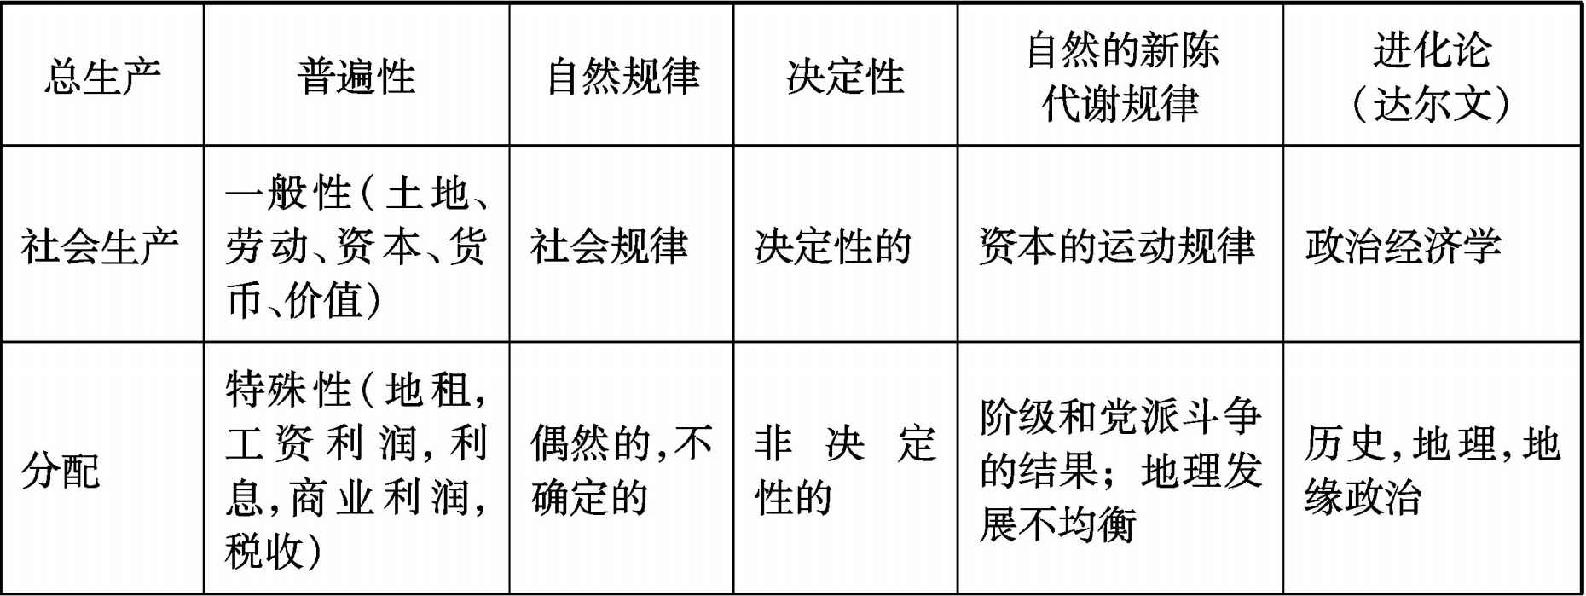
\includegraphics[scale=0.35]{david1.jpg}
\caption{马克思在《资本论》中采用的“弱三段论”分析框架}


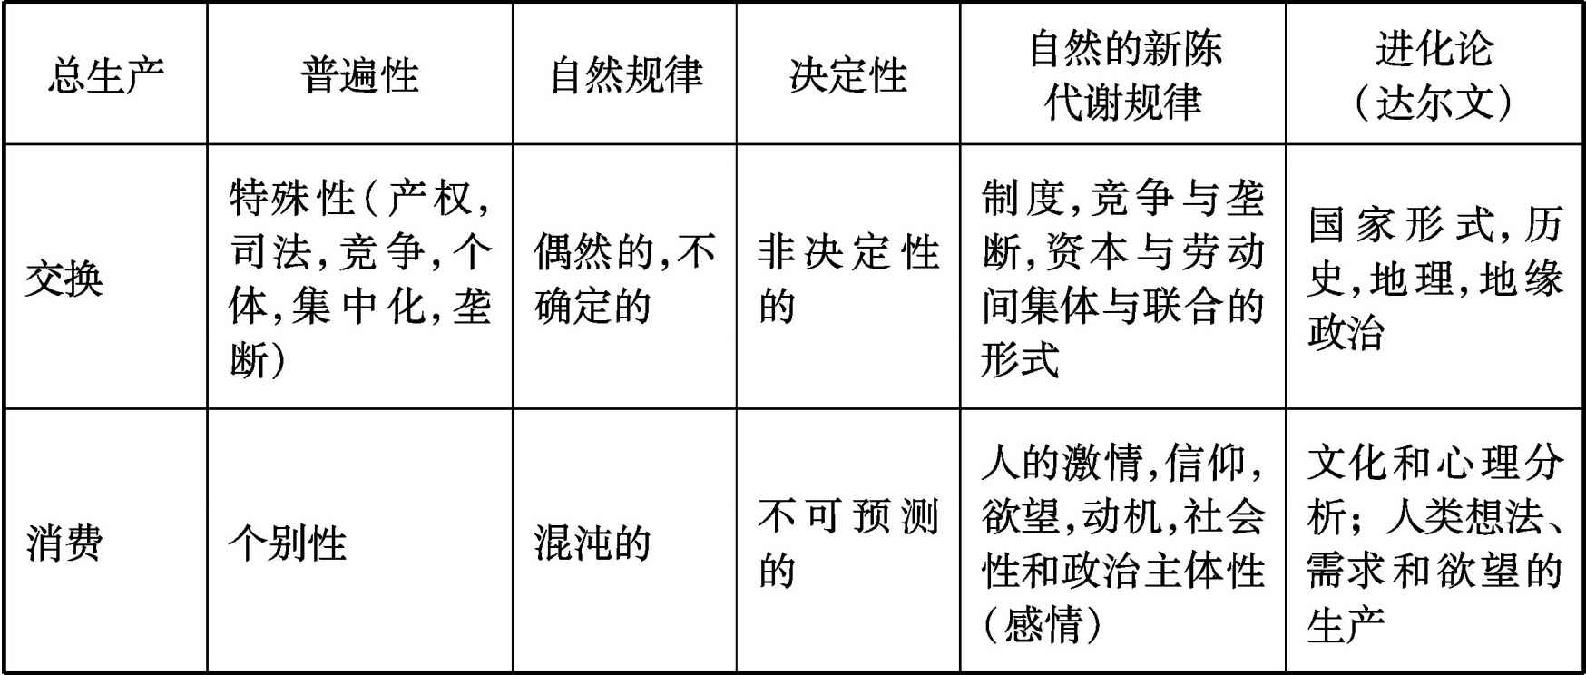
\includegraphics[scale=0.35]{david2.jpg}
\caption{续图1}
\end{figure}

尽管这个三段论“被公认为是一致的”,马克思说它还只是“肤浅的”。所以他拒绝了这个三段论,而是用辩证法研究了生产、分配、交换和消费怎样在构成资本主义生产方式的关系总体中结合起来。马克思对生产和消费、生产和分配、生产和交换的内在辩证关系进行了一系列讨论后得出了结论。生产、分配、交换和消费“构成一个总体的各个环节、一个统一体内部的差别\ldots{}\ldots{}不同要素之间存在着相互作用。每一个有机整体都是这样”。\pagescite[][37]{karlvol46a} 


马克思所想的资本主义生产方式的有机整体(总体)并不完全是黑格尔式的(尽管它来自于
对黑格尔概念的革命性改造,而非仅仅是简单地颠倒过来使用)。它的结构是生态系统的,
由葛兰西和列斐伏尔所说的不同时刻“总体”或德勒兹所说的不同时刻的“组合”的关系组成。马克思抱怨道:“对于一个黑格尔主义者来说,把生产和消费等同起来,是最简单不过的事。不仅社会主义美文学家这样做过,而且平庸的经济学家也这样做过。”\pagescite[][31]{karlvol46a} (Big Note)


读者也许期待马克思用辩证法和有机的理论来构建他的替代理论。但是从《资本论》的写作实践来看,即使他使用有机的思维和辩证的——关系性的分析来建构他的批判和探索另一种理论,很显然他最后还是遵循了古典政治经济学的三段论架构框架。他始终尽可能地贴近资产阶级关于生产一般的规律层次的概念,排除了具有“偶然性”和社会特殊性的分配和交换(直到在第三卷的最后部分才进行了讨论),至于混乱的消费的个别性当然更是如此。

在这里我要提出一点警告,这个排除有时是过分的(马克思应该做出说明)。(笔者注:马
克思对劳动力价值、在第三卷中“详细分析信用制度和它为自己所创造的工具(信用货币等),在我们的计划之外。在这里,只着重指出为说明资本主义生产方式一般的特征所必要的少数几点。”\pagescite[][350]{capital3} 


我最好的假设是,马克思根本的意图是以子之矛攻子之盾,用古典政治经济学自己的术语批判它本身。所以为了说明古典政治经济学的内在矛盾和不足,他不得不接受了这些术语的一般性质。因此如果资产阶级理论家事先假定了一个非强制的自由市场,那么马克思也需要这样做(就像他在第一卷第2章中所做的那样)。如果一般、特殊和个别之间的区别是资产阶级思维模式的基础,那么马克思也需要使用这个基础。这是我能给出的唯一答案,但还是不能完全让人满意,因为马克思接受了一些资产阶级的术语而拒绝了其他的。比如马克思在第一卷中没有涉及供给和需求或效用的问题(我们不久将看到他为什么这样做)。他从不对自己选择的逻辑进行解释。很明显他通篇都作出了这样的选择。

一般、特殊和个别这三个层次并不是故事的全部,还有第四个层次——普遍性——涉及与自然的
新陈代谢关系。马克思对古典政治经济学家把生产视作“包裹在独立于历史之外的永恒的自
然法则中”的做法表示了强烈反对。马克思反对把资本主义政治经济学“自然化”,从不放
弃任何抨击这种自然主义观点的机会(包括李嘉图学派和马尔萨斯学派认为利润率注定会下
降是因为自然资源的缺乏和地租上涨的观点)。马克思强调资本主义生产方式的一般性不能
用自然法则的普遍性解释。虽然马克思同意“资本主义生产”是规律般的一般性,他还是拒
绝以自然科学的方式将其理解为纯粹“自然”的东西。资本主义虽然是具有规律性的,但是
这些规律(包括那些关于私人财产关系的)是人类行为的产物。

为什么要赋予生产以优先权呢?马克思认为“生产既支配着与其他要素相对而言的生产自身,
也支配着其他要素。过程总是从生产重新开始”。这句奇怪的话是什么意思呢?\textbf{把
  支配自身的生产解释为产品和服务的物质生产,或是具体的劳动过程,甚至是商品的生产
  都是错误的。}非常不幸的是,这是个十分常见的误读,导致了对马克思认为社会关系、思
想、人类欲望等是由物质资料生产决定的说法的误解。这是生产主义和物质主义的误读,并
不是真正的马克思的历史唯物主义。(Big Note)


\textbf{在资本主义生产方式中占主导的生产是剩余价值的生产,剩余价值是社会性的,而
  不是物质性的关系。},在马克思宏伟的计划中,这意味着为他人生产剩余价值的社会需要
扭曲和支配了人的感觉器官通过劳动过程所能获得的解放的潜能。这个结果是对人类自身潜
在生产力和创造力的普遍异化。《政治经济学批判大纲》和《资本论》中一些最有说服力的
章节再三强调了这点。(笔者注:恩格斯致约·布洛赫(1890年9月21-22日)“根据唯物史
观,历史过程中的决定性因素归根到底是现实生活的生产和再生产。无论马克思或我都从来没
有肯定过比这更多的东西。如果有人在这里加以歪曲,说经济因素是唯一决定性的因素,那末
他就是把这个命题变成毫无内容的、抽象的、荒诞无稽的空话。”恩格斯同样强调了这点。
而经济基础决定上层建筑,上层建筑又反过来作用于经济基础是后来人对恩格斯这句话下面
部份的演绎,且过于决定论和片面化。)(Big Note)

简言之,通过资本循环进行的剩余价值的生产是规律般的资本主义生产方式的核心:没有剩余价值,就没有资本主义。这是马克思对古典政治经济学做出的根本性突破。马克思继续写道:

\begin{quotation}
交换和消费不能是起支配作用的东西,这是不言而喻的。分配,作为产品的分配,也是这样。而作为生产要素的分配,它本身就是生产的一个要素。因此,一定的生产决定一定的消费、分配、交换和这些不同要素相互间的一定关系。当然,生产就其单方面形式来说也决定于其他要素。\pagescite[][36-37]{karlvol46a} 

\end{quotation}

资本主义生产方式的“规律”事实上采取了以下形式:各种各样可能的、偶然的分配和交换
结构和多样化的消费体制在原则上都是可能的,只要它们不会过度限制或破坏规模不断扩大
的生产剩余价值的能力。\ldots{}\ldots{}从剩余价值生产的一般规律并不能直接推演出唯
一的分配模式、交换体系或特定的消费文化体制。但是——这是个很重要的“但
是”——它的可能性不是无限的。在任何时刻,包括与自然的关系,如果出现了过分地限
制或破坏剩余价值生产能力的情况,那要么资本将不复存在,要么总体关系必须作出全面调
整。这就是“决定”的含义。

供给和需求还有价格的波动对经济达到均衡状态很重要,但是均衡在哪里可以达到并不能用它们来解释。马克思在大多数情况下通过假设把这种扭曲排除在外,但有时因为系统的相关性他还是会把这些因素加入到思考中,比如在劳动价格问题上。

“竞争一般来说是资本贯彻自己的生产方式的手段”。竞争使资本的内在规律得到贯彻,使
这些规律对于个别资本成为强制规律。但是它并没有发明这些规律。竞争实现这些规
律”。\pagescite[][271]{karlvol46b}其他力量建立起资本运动的内在规律,竞争仅仅是执
行者和实施者,就像供给和需求那样。

\begin{quotation}
  资本主义生产的发展,使投入工业企业的资本有不断增长的必要,而竞争使资本主义生产
  方式的内在规律作为外在的强制规律支配着每一个资本家。竞争迫使他不断扩大自己的资
  本来维持自己的资本,而他扩大资本只能靠累进的积累。\pagescite[][683]{capital}

\end{quotation}

当垄断和寡头组织占据支配地位时,资本运动规律(甚至价值本身)会发生改变。这反映在20世纪60年代由保罗·巴兰、保罗·斯威齐还有法国共产党提出的(国家)垄断资本主义理论中。

但是,垄断阶段之后通常会进入另一个阶段,这时竞争的强制规律的恢复成为主要的政治关
切。20世纪70年代末资本主义世界的大部分国家普遍经历了这个过程。毕竟,这是新自由主
义的中心议程。资本家经常抱怨竞争是“破坏性的”,但是垄断很容易产生“滞胀”,就像
巴兰和斯威齐所说的那样。资本主义国家的政策经常试图在垄断(通过对经济“制高点”实
行国有化)和竞争(通过反兼并、反垄断立法,以及或情愿或不情愿地走向私有化和全球化
竞争)两者之间保持平衡。(Big Note)

操纵和调动人的欲望一直处在资本主义历史的中心,但马克思把它排除在了政治经济学之外,认为这属于历史研究的范畴。不过,它并非完全处于理论思考之外。(Big Big Note)


例如劳动者可以选择怎样花钱和用钱买什么,因此知道他们的想法、需求和欲望就变得非常重要。马克思认为,为了在不同的经济部门之间保持必要的均衡,资产阶级必须操纵大众消费,以使工人的消费相对于资本主义积累是“合理的”。资产阶级的博爱于是经常体现为教导劳动者的消费习惯,使之有利于积累。奢侈品和工资品之间的差别也变得很重要。(Big Big Note)

因此,马克思留给我们的一部分工作是对当代的消费主义找到比目前更好的解释。传统的政
治经济学研究的方法论在解释消费方面不太有效(马克思反对把太多消费的例子加入到政治
经济学领域中可能也是出于这个原因)。这同样适用于生产性消费——在商品生产的劳动过程
中用劳动消费原材料。控制劳动者在工作中的个性的困难已经被认识到了(尤其是在马里奥·特
隆蒂和安东尼奥·奈格里的作品中),正是这种个性蕴含着巨大的革命性潜力。

马克思认为消费是个别性而不是一般性也是因为这个道理。但是,马克思的历史著作的最终目的是把资本主义生产方式作为一个演进的有机整体来理解(与强调规律的政治经济学相反),因此任何对当代形势加以理解的尝试,都要求我们把消费、政治主体性和个体的审美、文化、政治偏好加入到研究框架中——作为政治经济学分析的基础和补充,而不是作为替代品。

在一般性方面的严格限制让马克思对资本的理解超越了他所在的时代的历史特殊性。这也是
为什么我们至今仍能阅读马克思著作的原因——即使是第二卷——而且还能够理解很多
他想要表达的内容。另一方面,很难将这个框架直接用于分析我们的现实状况,这也是我们
将要进行的工作。

\chapter{资本循环(第二卷 第1—3章)}

\begin{figure}
\centering
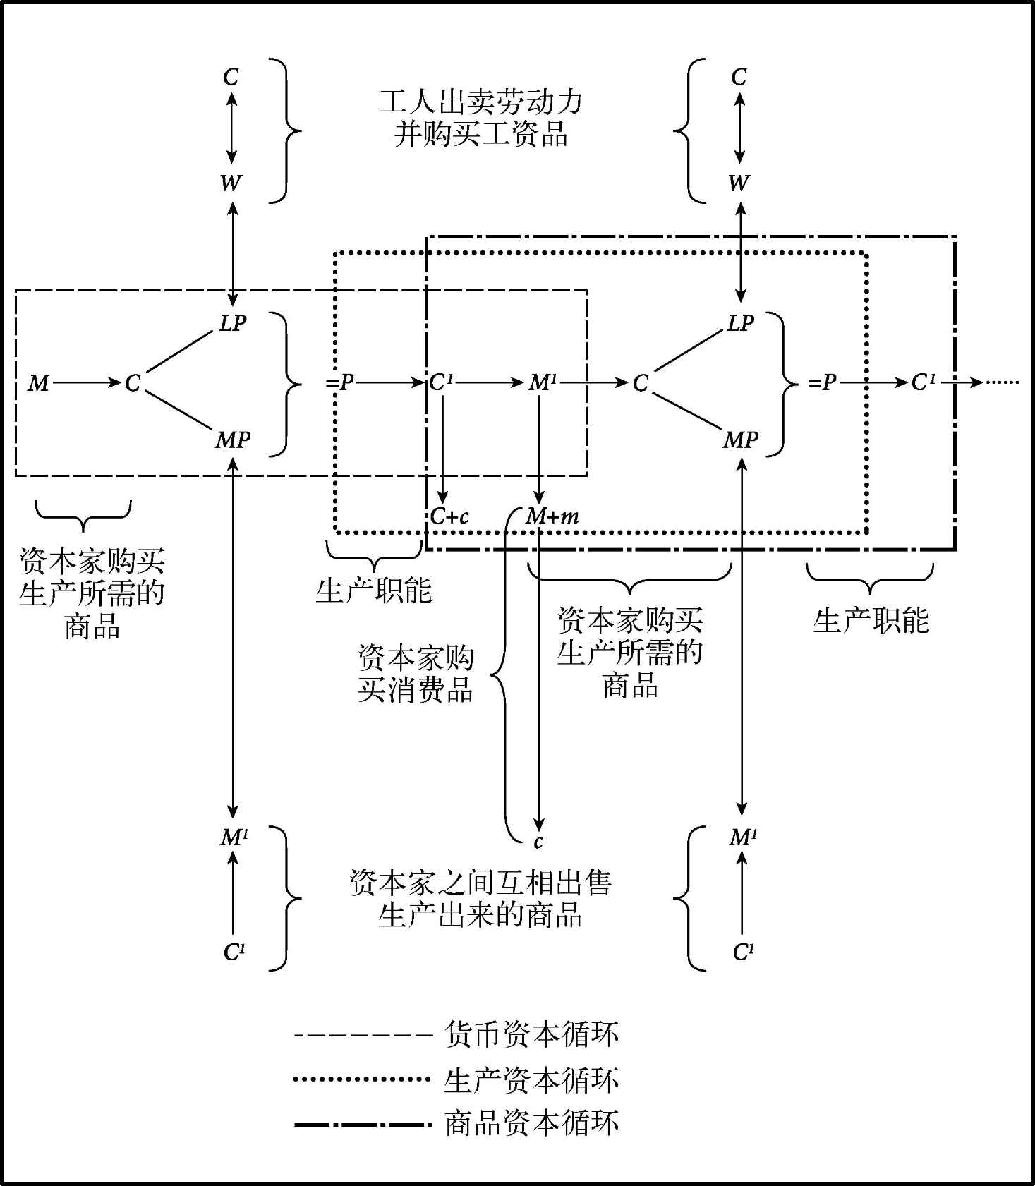
\includegraphics[scale=0.35]{david3.jpg}
\caption{产业资本循环的总公式,三个不同循环}
\end{figure}

在货币形态,资本可以像蝴蝶一样到处自由地“飞翔”;在商品形式上,资本就像毛虫一样,到处寻找想要、需要或是渴望得到它,有支付能力并最终消费它的人;作为劳动过程,资本植根于“生产的隐秘之处”(马克思在第一卷中提到),在这里,物质活动将自然要素转化为商品的生产。

资本在不同形态下进行的空间和地理运动的差异,对于理解我们统称为“全球化”的过程有
重要启发。

\begin{quotation}
  在生产危机和商业危机中称为货币危机的那一刻暴露得特别明显。这种货币危机只有在一
  个接一个的\textbf{支付的锁链}和抵消支付的人为制度获得充分发展的地方,才会发生。
  当这一机制整个被打乱的时候,不问其原因如何,\textbf{货币就会突然直接地从计算货
    币的纯粹观念形态转变成坚硬的货币}。这时,它是不能由平凡的商品来代替
  的。

  商品的使用价值变得毫无价值,而商品的价值在它自己的价值形式面前消失了。昨天,资
  产者还被繁荣所陶醉,怀着启蒙的骄傲,宣称货币是空虚的幻想。只有商品才是货币。今
  天,他们在世界市场上到处叫嚷:只有货币才是商品!他们的灵魂渴求货币这惟一的财富,
  就像鹿渴求清水一样。在危机时期,商品和它的价值形态(货币)之间的对立发展成绝对
  矛盾。\pagescite[][161-162]{capital} (Big Note)

  使劳动力的使用权归属于买者。而使用这种劳动力的界限,和劳动力本身价格的再生产所
  必需的劳动量的界限,又决不是一致的。资本关系所以会在生产过程中出现,只是因为这
  种关系在流通行为中,在买者和卖者相互对立的不同的基本经济条件中,在他们的阶级关
  系中本来就已经存在。不是由于货币的性质产生了这种关系;相反,\textbf{正是由于这
    种关系的存在,单纯的货币职能才能转化为资本职能。}\pagescite[][39]{capital2}

  要使资本能够形成并且能够支配生产,需要商业发展到一定的阶段,因此也需要商品流通
  从而商品生产发展到一定的阶段。……只有在资本主义生产的基础上,商品生产才表现为
  生产的标准的、占统治地位的性质。\pagescite[][40]{capital2} (Note)

  那些造成资本主义生产的基本条件,即雇佣工人阶级的存在的情况,也促使一切商品生产
  过渡到资本主义的商品生产。资本主义的商品生产越发展,它对主要是直接满足自己需要
  而只把多余产品转化成商品的每一种旧生产形式,就越发生破坏和解体的作用。\pagescite[][43]{capital2} 

  我们在重商主义体系的辩护人那里,发现了这样冗长的说教:资本家个人只应该和工人一
  样消费,资本家国家应该把它们的商品让给其他比较愚昧的国家去消费和进行消费过程,
  而相反地应该把生产消费当作自己的终生事业。这种说教在形式上和内容上往往使人想起
  教父们类似的禁欲诫条。\pagescite[][70]{capital2} (Big Note)

\end{quotation}
有一些人,例如凯文·菲利普斯,相信我们在过去十几年里经历了重商主义阶段,而美国担当的正是最愚昧的国家的角色(进行债务支撑的消费主义),中国人和德国人则以美国消费者为代价储蓄和积累了大量的贸易盈余。奥巴马当局在出席2010年秋季在首尔举行的G20峰会时,提议减少全球体系中的贸易不平衡,中国和德国是反对这个提议的主要国家。所以,某种形式的重商主义确实存在,而且状况良好——美国似乎仍然乐于担当最愚昧的国家的角色。(Big Note)

\begin{quotation}

  只要把这种形式(货币资本循环)不是当作循环形式的一种,而是当作惟一的循环形式,
  它的虚幻的性质以及与它相适应的虚幻的解释就会存在。但是,它本身已经指出其它的形
  式。\pagescite[][72]{capital2} 

  货币资本转化为生产资本,就是为生产商品而购买商品。只有消费是这种生产消费(剩余
  价值),它才进入资本本身的循环。…… 这样一种由剩余价值的生产所决定的用商品代替
  商品,和本来的产品交换(只是以货币为中介)完全不同。可是,经济学家们竟以此证明
  生产过剩是没有可能的。\pagescite[][87]{capital2} 

\end{quotation}

需要着重指出一点,如果工人将收入用来赌博(甚至是储蓄),而不是用来购买商品,那么循环过程的连续性就会遭到破坏。因此第二卷最后关注建立工人阶级的“合理消费”,将之作为稳定积累的条件的问题

\begin{quotation}
  商品的潮流一浪一浪涌来,最后终于发现,以前涌入的潮流只是表面上被消费吞没……以
  前涌入的商品还没有变成现金,支付期限却已经到来。商品持有者不得不宣告无力支付,
  或者为了支付不得不给价就卖。这种出售同需求的实际状况绝对无关。同它有关的,只
  是\textbf{支付的需求},只是把商品转化为货币的绝对必要。于是危机爆发
  了。\textbf{它不是表现在消费需求,即个人消费需求的直接缩减上,而是表现在资本对
    资本的交换,即资本再生产过程的缩减上。}\pagescite[][89]{capital2} (Big Big Note)

\end{quotation}

在个人消费领域表现出来的工人和资本家的有效需求不足,事实上可能是由于生产资料的购买和售卖的循环过程出现了问题。(Big Big Note)

关于工人阶级的有效需求和消费,马克思在第二卷中有两处看似非常矛盾的论述:
\begin{enumerate}
\item {\kaishu 资本主义生产方式中的矛盾:工人作为商品的买者,对于市场来说是重要的。
    但是作为他们的商品——劳动力——的卖者,资本主义社会的趋势是把它的价格限制在最低
    限度——还有一个矛盾:资本主义生产全力扩张的时期,通常就是生产过剩的时期;因为
    生产能力从来没有能使用到这个程度,以致它不仅能够生产更多的价值,而且还能把它
    实现。商品的出售,商品资本的实现,从而剩余价值的实现,不是受\textbf{一般社会
      的消费需求的限制},而是受\textbf{大多数人总是处于贫困状态、而且必然总是处于
      贫困状态的那种社会的消费需求的限制}。\pagescite[][350]{capital2} }

 
\item {\kaishu 认为危机是由于缺少有支付能力的消费或缺少有支付能力的消费者引起的,
    这纯粹是\textbf{同义反复}。除了需要救济的贫民的消费或“盗贼”的消费以外,资本
    主义制度只知道进行支付的消费。商品卖不出去,无非是找不到有支付能力的买者,也
    就是找不到消费者(因为购买商品归根结底是为了生产消费或个人消费)。但是,如果
    有人想使这个同义反复具有更深刻的论据的假象,\textbf{说什么工人阶级从他们自己
      的产品中得到的那一部分太小了,只要他们从中得到较大的部分,即提高他们的工资,
      弊端就可以消除},那么,我们只须提出,危机每一次都恰好有这样一个时期做准备,
    在这个时期,工资会普遍提高,工人阶级实际上也会从供消费用的那部分产品中得到较
    大的一份。按照这些具有健全而“简单”(!)的人类常识的骑士们的观点,这个时期
    反而把危机消除了。因此,看起来,资本主义生产包含着各种和善意或恶意无关的条件,
    这些条件只不过让工人阶级暂时享受一下相对的繁荣,而这种繁荣往往只是危机风暴的
    预兆。\pagescite[][456-457]{capital2} }
\end{enumerate}

第二个论述与第2章的精神更为一致,所以很明显,马克思认为从生产资本的角度展开的论述
具有更普遍的重要性。于是我们就面临一个难题:该追随哪个观点?我自己的想法是(你也
可以有自己的想法),这种情形可以出现,正如20世纪60年代末70年代初那样,劳动所得占
国民产出份额的上升,即便不是全球资本主义危机的根本原因,也至少是其先兆。但是,不
可能用这个观点来分析2007—2008年的经济崩溃。\textbf{工人阶级的分配份额,无论是过高
  还是过低,虽然有重要影响,但还不足以解释资本的危机倾向}。

\begin{quotation}
在P……P`中,P`所表示的,不是剩余价值被生产出来,而是生产出来的剩余价值已经资本
化,就是说,资本已经积累。\pagescite[][93]{capital2} (Big Big Note)

一个在资本循环之外完成的、为使剩余价值转化为实际执行职能的资本所进行的职能上确定
的预备阶段……只要它停留在贮藏状态中,它就还不是执行货币资本的职能,而是闲置的货
币资本;不是像前面所说的那种职能中断的货币资本,而是还不能执行职能的货币资本。\pagescite[][97]{capital2} 

\end{quotation}

在将特殊形式的价值和剩余价值转化成作为一般等价物的货币的困难之外,我们现在再加上
另一个困难:在市场中寻找必要的商品以\textbf{满足特定劳动过程中的生产性消费的需要}。
资本家必须依靠其他资本家生产自己所需的生产资料。因此,主要是在商品资本的循环中,
我们面临资本家之间特殊的相互关系和相互依赖的难题。随着第二卷内容的展开,越来越明
显的是,这种资本家之间的相互关系受到\textbf{充足供应(adequate supply)危机}的可
能性的困扰,更明显的问题可能是由有效需求不足引起的危机。

在生产率不变的情况下,规模扩大的再生产(撇开对外贸易)只有在剩余产品的待资本化的部分已经包含追加生产资本的物质要素时才能进行。\pagescite[][114]{capital2} 

\begin{quotation}
  正因为W′……W′ 循环在进行中要以另一个在W(=A+ Pm)形式上的产业资本为前
  提(并且Pm还包括各种其他资本,用我们的例子来说,包括机器、 煤炭、 润滑油等等),
  所以,这个循环本身就要求我们不仅把它看作循环的\textbf{一般}形式,即能够用来考察
  每一个\textbf{单个}产业资本 ( 第一次投资的场合除外) 的社会形式,因而不仅看作一
  切单个产业资本共有的运动形式,而且同时看作各单个资本的总和即资本家阶级
  的\textbf{总资本的运动形式},在这个运动中,每一个单个产业资本的运动,都只表现为
  一个部分运动,和其他部分运动交织在一起,并且受它们制
  约。\pagescite[][112]{capital2} (Big Big Note)

\end{quotation}
商品资本的循环很特别,它允许我们着眼于整体经济中的剩余价值和剩余产品(价值和使用
价值)的总的流动。……这种思维模式的先驱是魁奈。

在其他循环中,我们可以只关注个别的产业资本,而不必关心加总的情形。加总的情形只在商品资本的循环中出现。

\chapter{循环的三个公式和资本流动的连续性(第二卷 第4—6章)}

\begin{quotation}
  在一个不断回转的循环中,每一点都同时是出发点和复归点。……不仅每一个特殊的循环
  都把其他的循环作为前提( 包含在内),而且一种形式的循环的反复,已经包含着其他形式
  的循环的进行。 因此,全部区别表现为单纯形式上的区别,或者说,表现为单纯主观上
  的、 只对考察者才存在的区别。

资本在它的任何一种形式和任何一个阶段上的再生产都是连续进行的,就像这些形式的形态变化和依次经过这三个阶段是连续进行的一样。可见,在这里,总循环是资本的三个形式的现实的统一。\pagescite[][117]{capital2} 

\end{quotation}

这里强调的是资本在这三种循环运动中的连续性、继起性、并存性和流动性。问题的反面则是阻碍和可能的中断。“资本的循环过程是不断的中断,是离开一个阶段,进入下一个阶段;是抛弃一种形式,存在于另一种形式;其中每一个阶段不仅以另一个阶段为条件,而且同时排斥另一个阶段。”\pagescite[][118]{capital2} (Big Big Note)

“那些把价值的独立化看作是单纯抽象的人忘记了,产业资本的运动就是这种抽象的实
现”。\pagescite[][122]{capital2} “独立化”暗示了一个特别的问题。价值可能是一个
抽象概念,但是它却有真实的影响(或者用第一卷的话来说,价值是“幽灵般的对象性”)。
(Big Note)

\begin{quotation}
  如果社会资本的价值发生\textbf{价值革命},他个人的资本就可能受到这一革命的损害而
  归于灭亡,因为它已经不能适应这个价值运动的条件。价值革命越是尖锐,越是频繁,独
  立化的价值的那种自动的、以天然的自然过程的威力来发生作用的运动,就越是和资本家
  个人的先见和打算背道而驰,\textbf{正常的生产过程就越是屈服于不正常的投机,单个
    资本的存在就越是要冒巨大的风险。}因此,这些周期性的价值革命证实了它们似乎应该
  否定的东西,即证实了价值作为资本所经历的、通过自身的运动而保持和加强的独立化。(Big Big Note)

\end{quotation}

这完全可以算是对我们现在所谓的“去工业化”导致的资本贬值危险的理论再现。
从20世纪80年代起,一股巨大的工厂倒闭浪潮冲击了底特律、匹兹堡、巴尔的摩、谢菲尔德、
曼彻斯特、埃森、里尔和都灵等老工业城市。这种现象不只在发达资本主义国家出现,孟买
的传统纺织业区和中国北部的老工业基地同样遭受了猛烈的冲击和损失。所有集中于工业生
产的社区几乎都在一夜之间被摧毁了。比如谢菲尔德在20世纪80年代的三年时间内,失去了
大概六万个钢铁生产的工作岗位,到处是荒凉的景象。当人们寻找原因时,却被告知,这一
切都是由一股被称为“全球化”的神秘力量引起的。当工会和社会运动抗议并寻求遏止工作
和谋生手段流失的途径时,却被告知这种神秘的力量是无法避免和不可阻挡的。(Big Big Note)

更正式的表述就是:个别的资本家为了追求相对剩余价值而组织价值的生产,但这样做产生
的新的价值关系反过来会摧毁他们自己。资本不仅生产自身统治的手段,还生产毁灭自己的
手段。……但是他们不对资本主义制度感到愤怒,反而对外国生产者、移民者、投机者和其
他一些仅仅是资本运动的内在规律中秘密的、隐藏的当事人感到愤怒。(Big Big Note)

\begin{quotation}
  只有各种干扰在循环反复中被排除,过程才能够在事实上正常进行;\textbf{干扰越大,
    产业资本家就必须持有越是大量的货币资本},才有可能等到干扰被排除;因为随着资本
  主义生产的进展,每一个单个生产过程的规模会扩大,预付资本的\textbf{最低限量也会
    随之增加},所以除了其他情况外,又加上这个情况,使\textbf{产业资本家的职能越来
    越转化为各自独立或相互结合的大货币资本家的垄断}。\pagescite[][124]{capital2}(Big Big Note)

  (产业资本的循环)是和各种极其不同的社会生产方式的商品流通交错在一起的……不论
  商品是建立在奴隶制基础上的生产的产品,还是农民的产品(中国人,印度的佃农),还
  是公社的产品(荷属东印度),还是国家生产的产品(如在俄罗斯历史早期出现的以农奴
  制为基础的国家生产),还是半开化的狩猎民族的产品等等,它们都作为商品和货币,同
  表现产业资本的货币和商品相对立。\pagescite[][126]{capital2} 

  资本家以货币形式投入流通的价值,小于他从流通中取出的价值,这是因为他以商品形式
  投入流通的价值,大于他以商品形式从流通中取出的价值。既然他只是作为资本的人格化,
  只是作为产业资本家执行职能,他供给的商品价值,总是大于他需求的商品价值……资本
  家的供给和需求的差额越大,就是说,他所供给的商品价值越是超出他所需求的商品价值,
  资本家的资本增殖率就越大。他的目的,不在于使二者相抵,而是尽可能使它们不相抵,
  使他的供给超出他的需求。就单个资本家来说是如此,就资本家阶级来说也是如此。\pagescite[][133]{capital2} 

\end{quotation}

过剩资本的处置或吸收问题(卢森堡提法比较重要,马尔萨斯、卢森堡、马克思关于这方面
的论述也可参考上一卷的笔记):购买剩余价值的需求是从哪里来的呢?如果这只是寻找更
多货币的问题,那么在某处的某人(例如我们时代的联邦储备系统;对马克思来说是黄金生
产者,他随后考虑了他们潜在的作用)能简单地满足这个要求。\textbf{但是我们必须从价
  值而不是货币的范畴来解决这个问题。}如果剩余价值在交换中实现,那么我们必须解释最
终与剩余价值交换的等量价值是从何而来的。从理论上说,我们得回答这个问题,但是不能在资本主义范围外寻求答案(例如马克思在本章前面提到的需求和供给的非资本主义来源),也不能假设存在一个专门进行挥霍性消费的阶级。

对于马克思的看法,这里有一个可能的解释。在这一章的开头,他说“过程的所有前提都表
现为过程的结果,表现为过程本身所产生的前提。每一个因素都表现为出发点,经过点和复
归点”。\pagescite[][116]{capital2} 或者,像马克思一开始说的那样,前提(资本家的
有效需求)现在表现为结果(剩余价值的占有)。在简单再生产中这可能会起作用,但是,
由这些章节的主要观点可知,这个过程不太可能不受任何干扰和中断地顺利进行下去。

但是,如果资本家如此行事,那么他就成了“非资本家”,“他作为非资本家花掉的,不是
花在他作为资本家的职能上,而是花在他的私人需要或享受上”。马克思还说:“这个假定
等于假定资本主义生产不存在,从而假定产业资本家本身不存在。因为只要假定发挥作用的
动机是享受,而不是发财致富本身,资本主义就从根本上被废除了。”享受和发财致富的区
别似乎对马克思的推理很重要。说资本主义是建立在个人自身的享受欲望的基础上的,就违
背了马克思在第一卷第24章中论证的观点。在那里,他认为资本主义基于“为了生产而生产
和为了积累而积累”,是独立于资本家的个人欲望之外的。尽管总存在消费和享受的欲望与
追加投资的必要性相互冲突的“浮士德时刻”,但是竞争的强制规律迫使资本家无可奈何地
选择了后者。所以,把资本家假定成贪恋消费品的个体,并将其作为资本积累的驱动力,是
不充分的;假定资本家的驱动力是通过攫取货币占有更大的社会权力,也是不充分的(尽管
我们以后会看到,与这个动机有一定的关系)。资产阶级的历史任务就是不断地进行资本积
累。“在技术上也是不可能的。资本家不仅必须形成一个准备资本,以应付价格的变动并等
待买卖上最有利的行情;他必须积累资本,以扩大生产,并把技术进步合并到他的生产机体
中去”。\pagescite[][137]{capital2}

当部分剩余价值被再投资于扩大再生产时,上文提出的解决有效需求问题的办法就更不可行
了。资本家不仅要为购买和实现最初循环的剩余价值提供必要的资金,而且得寻找更多的资
源来实现再投资所生产的剩余价值。因此,问题将会一直存在。

我宁愿大略说出我对马克思论点的理解。资本家的消费分为两种类型:个人消费(必需品和奢侈品)和生产性消费。后者要求将初始资本收回,用于另一轮的剩余价值生产,并追加投资于扩大再生产,这意味着对更多的生产资料和额外雇佣的劳动力所需的消费资料的需求(假设没有劳动节约型的技术改进)。竞争的强制规律推动了扩大再生产(因此,重点是发财致富,而不是享乐)。所以,来源于\textbf{明天的}扩大生产的需求(加上资产阶级消费),为今天生产的过剩商品提供了市场。

实际上,需要用出售明天的产品得到的货币支付今天生产的剩余价值。资本家的供给和需求
间暂存的缺口只能在信用货币(马克思在第二卷中刻意回避这个问题)的帮助下填补。实际
上,资本家没必要向别人借钱。他们只需要打个欠条,先买后付——这种做法由来已久了。因
此,\textbf{资本积累和债务积累紧密相连,谁也离不开谁。}遏制债务进一步发展(像共和党
在2011年做的那样),实际上是一场终结资本主义的战斗。这就是为什么紧缩政策,如果无
限期执行的话,不仅会阻碍经济增长,而且最终将导致资本主义的崩溃。(Big Big Note)

马克思也指出,资本主义的商品生产必须按“生产一般”的方式进行,并且和 “非资本主义的生产过程”没有任何特殊的物理属性上的差异。

资本是生产——理解为\textbf{剩余价值的生产(不是物质生产)},它支配着分配、交换和消
费的所有环节,更重要的是,支配着生产的物质过程本身。\textbf{资本的再生产总是被理
  解为劳动和资本的阶级关系的再生产}(在第一卷第23章中解释得很清楚)。(Big Note)

在所谓的“部分无产阶级化”的情况下,全球劳动力中的很大一部分人拥有一些土地和其他
家族或血缘资源,当他们遭遇失业、生病或残疾时就会回到这种状况。例如,在当代中国就
是这种情况,很多社会再生产的成本都是由农村地区承担的。更为冷酷无情的是,美国的农
业综合企业就是以这种方式把社会再生产的成本转嫁到墨西哥身上的:雇用非法移民来从事
有致癌作用的杀虫剂的喷洒工作,直到他们病入膏肓,从而不得不返回墨西哥农村,在那里
接受照顾或者死去。

资本的特性存在于有利于创造剩余价值的生产中的阶级关系之中,其一般性存在于由货币、
生产和商品资本循环构成的产业资本的循环过程之中。

因此,认为在不对其他循环的运行进行根本变革的条件下,就可以在生产领域实现深刻变革
的想法只能是妄想。向社会主义或共产主义过渡,不仅需要通过激烈的斗争去消灭生产中的
阶级关系,还需要逆转或者重建其他循环,以表明货币化、商品化和劳务的交换是怎样实行
变革,为生产中的联合劳动提供支持的。(Big Big Note)

这个结论在这些漫长而往往自负的历史中找到了支持:尝试在非资本主义方式的基础上重新
改造资本主义生产,特别是在联合劳动的口号下。工人控制、自我管理、工人自治和合作工
厂的尝试(20世纪70年代在欧洲和2001年经济危机后在阿根廷兴起的那种)一直受到怀有敌
意的商人和金融资本的控制力的威胁,在某些情况下一度被摧毁了。工人控制和工人自治的
梦想,经常在货币和商品资本力量,以及规训它们的交换价值规律的岩石上撞得粉碎。价值
增殖从而榨取剩余价值的驱动力难以阻挡。显著的例子是1956年西班牙法西斯专政时期巴斯
克县的工人合作社蒙德拉贡,它之所以能长期存在,部分是因为它建立了属于自己的信用机
构和市场机制,从而在三个循环中贯彻了自己的政治主张。它继续存在并且繁荣发展着,其
两百家企业中的大部分仍把参与者的回报差距控制在3∶1(相比之下,美国公司是400∶1,
甚至更高)。有人批评蒙德拉贡越来越依赖外包合同,因此是通过剥削其他地区而生存)。(Note)

联合劳动形式面对的困难主要来自一直存在的资本主义的价值规律。就像我们之前看到的,
价值规律支配并常常摧毁个别资本。一旦进入由价值规律支配的世界,企业就得服从这些规
律的规训力量。远离这种规训力量即使不是不可能的,也是很困难的。为了生存,蒙德拉贡
和那些在阿根廷复兴的工厂不得不寻找与价值规律相妥协的方式。这使我们得出了一个至少
表面上令人气馁的一般性结论,马克思已经在他对资本贬值和去工业化的分析中使我们为这
个结论做好了准备:不废除资本的运动规律和支撑这些规律的价值规律的无形却客观的力量,
就不能废除生产中的劳资阶级关系。但是马克思经常被历史转变的协同演化理论所吸引。如
果我们在这里加入协同演化理论的轮廓,那么一种反资本主义斗争的策略就浮现出来了。尽
管劳动和资本的阶级关系处在资本定义的核心,它被深深的嵌入到了循环过程的其他方面之
中,以至于不废除或者取代它旁边的支撑物就很难消除它。尽管我们仍然相信联合劳动、工
人自治和自我管理的原则,也为尝试实行这样的生产和生活方式的漫长的斗争史感到光荣,
我们还是得面对社会变革的所有其他方面,它们是把全社会从资本的统治下解放出来所必需
的。

对于生产性和非生产性劳动之间的区分,在没有一个明确的核算上的解决方案时,我们面对的难题就是:如果既要保留马克思的直觉洞察力,又要承认实施这种区分的困难性(不可行性?),我们该怎样继续研究下去?

如果连续性是唯一的顾虑,那么我们就可以说,生产、流通和实现过程的所有劳动(也可以
延伸到用于劳动力再生产的家庭劳动)都是维持并再生产资本的总体劳动的一部分。换句话
说,我们可以认为所有参与产业资本循环的劳动者都算生产性工人。但是在马克思看来,这
将会粉饰和掩盖一些重要的东西。

反过来,我们可以推知,如果施加在这些扣除额(或者不能促进资本循环运动加速)上的权
力过大的话,危机可能会发生。如果所有权力都在货币资本家(金融家)和商业资本家(商
人)手里,那么它会对这部分资本最终依赖的价值生产造成什么样的影响呢?例如,2007年
后爆发的全球经济危机,可能是因为非生产性的资本和商品循环(例如高盛和沃尔玛)攫取
了过多的(正如我们将要看到的,绝大部分是虚拟的)利润,吸干了生产活动的能量;相反,
也可能是因为生产循环的状况严重恶化,刺激资本涌入了非生产性资本和商品循环中,通过
掠夺而不是生产来进行资本积累。(Big Note)

\begin{quotation}

显然,生产时间和劳动时间越吻合,在一定时期内一定生产资本的生产效率就越高,它的价值增殖就越大。因此,资本主义生产的趋势,是尽可能缩短生产时间超过劳动时间的部分。不过,资本的生产时间虽然可以和它的劳动时间不一致,但前者总是包含后者,而且超过的部分本身就是生产过程的条件。\pagescite[][141]{capital2} 

流通时间的延长和缩短,对于生产时间的缩短或延长,或者说,对于一定量资本作为生产资本执行职能的规模的缩小或扩大,起了一种消极限制作用。资本在流通中的形态变化越成为仅仅观念上的现象,也就是说,流通时间越等于零或近于零,资本的职能就越大,资本的生产效率就越高,它的自行增殖就越大。例如,假定有一个资本家按订货生产,因此他在提供产品时就得到支付,又假定支付给他的是他自己需要的生产资料,那么,流通时间就接近于零了。\pagescite[][142]{capital2} 

\end{quotation}
因此,生产资料供给的地理和空间条件给资本主义生产施加了限制,因为把生产资料运输到劳动进行的生产地点需要耗费时间。……为了获得生产所必需的使用价值,资本家要面对各种潜在的供给约束和成本。他们还得面对由其他资本,以及具有地缘政治雄心的国家权力所施加的约束。

\begin{quotation}
过程越是按社会的规模进行,越是失去纯粹个人的性质,作为对生产过程的监督和观念上的总括的簿记就越是必要;因此,簿记对资本主义生产,比对手工业和农民的分散生产更为必要,对公有生产,比对资本主义生产更为重要。\pagescite[][152]{capital2} 

\end{quotation}
表面上是流通的过程也可以创造一些价值。这种互相掺杂的情况使核算噩梦变得更糟:把商品放在容器中会增加它的价值,而它待在货栈里的时间则要从价值中扣除(例如,货栈的租金)。

我自己的结论是,放弃会计核算,转而集中于分析加速运动、库存费用管理等做法的实质影响。马克思已经说明,这些做法对于资本主义发展来说都是极端重要的。当我们把交通运输和通讯的问题,及其暗含的空间生产问题纳入进来时,这些问题就更加重要了。

商品在空间上的流通,即实际的移动,就是商品的运输。运输业一方面形成一个独立的生产部门,从而形成生产资本的一个特殊的投资领域。另一方面,它又具有如下的特征:它表现为生产过程在流通过程内的继续,并且为了流通过程而继续。\pagescite[][170]{capital2} 

\begin{quotation}
  \textbf{知识和技能的积累,社会智慧的一般生产力的积累,就同劳动相对立而被吸收在
    资本当中,从而表现为资本的属性,更明确些说,表现为固定资本的属性,}只要固定资
  本是作为真正的生产资料而加入生产过程。因此,机器体系表现为固定资本的最恰当的形
  式,而固定资本——就资本对自身的关系来看——则表现为资本一般的最适当的形
  式。\textbf{另一方面,就固定资本被束缚在自己一定的使用价值的存在中这一点来看,
    它是不符合资本的概念的,}因为作为价值来说,资本对采取任何特定的使用价值形式都
  是无所谓的,它可以把任何一种使用价值形式作为自己一视同仁的化身来加以采用或者抛
  弃。从这方面来看,从资本对外部的关系来看,流动资本同固定资本相比表现为资本的适
  当形式。\pagescite[][210]{karlvol46b}(Big Note)

\end{quotation}

我们已经多次看到,\textbf{连续性、流动性和加速}是资本流动的本质特性,但是现在我们
遇到一个范畴:固定资本的目的是促进流动,但是它本身是固定而不是流动的。

我认为矛盾是这样的:资本在一个时点创造了一整套适应其需要的景观,而在未来的某一时点,为了适应资本积累永恒的扩张的力量,会破坏它并重新建立一套新的景观。资本或者在别处,或者在旧的废墟上建立新的地理景观;留下的是去工业化的或废弃的景观,它们是孤立和破败的。这就是熊彼特所说的“创造性毁灭”。这一过程周期性地使资本循环和积累的地理景观发生贬值和变革——以惊天动地的方式。(Big Big Note)

原则上(尽管实际中并不总是这样),固定资本一直是永远对立的资本—劳动关系之外的一个常见的危机来源。危机在固定性不能适应扩张性的运动时发生。后者不得不打破已经固化的那部分资本所施加的限制。随着高度流动的货币资本流向别处,结果是大量固定资本的贬值。(1970年以来的去工业化留下了很多荒废的工厂、仓库和破败的基础设施——甚至衰退的城市,比如底特律)。(Big Big Note)

只被生产地消费,不能进入个人消费……在它完全损耗以前一直保持独立的形式。运输工具则例外。运输工具在它执行生产职能、从而停留在生产领域时产生的那种有用效果即场所变更,同时可以进入个人消费,例如旅客的个人消费。这时,旅客使用运输工具就像使用其他消费资料一样,也要支付报酬。\pagescite[][178]{capital2} 

我对这种例外情况很感兴趣,它意味着“场所变更”(从而,空间关系的生产)的有用性不仅适用于生产过程(原材料的移动),也适用于消费(人的移动)换句话说,“场所变更”的生产本身就是一种商品,不论谁使用它,也不论是为了什么目的(进一步的生产或者最终消费)。

\begin{quotation}
同一物品可以时而成为生产资本的组成部分,时而属于直接的消费基金。例如,一所房子,用作劳动场所,是生产资本的固定组成部分,用作住宅,就根本不是资本的形式,而只是一所住宅。在许多场合,同一些劳动资料,可以时而充当生产资料,时而充当消费资料。\pagescite[][227]{capital2} 

\end{quotation}
一个没有飞机起飞的机场是没有价值的。但是,没有机场的飞机也是没有价值的。注意,在
这个例子中很明显的是,可移动的固定资本形式(包括它们所携带的在市场上流通的商品资
本)在地理上的移动模式,受到另一些固定资本的增殖要求的限制——这些通常数额巨大的固
定资本被固定在了某个地方。不可移动的固定资本价值的收回,取决于运动中的资本对特定
地点的不可移动资本的使用。这产生了诸如城市间竞争的现象——将高度流动性的资本吸引并
保留在城市中(往往以对私人企业大量的公共补贴告终)。

\begin{quotation}
  可以利用的空间。有些建筑物可以加高几层;有些建筑物必须横向扩张,这就要有更多的
  地皮。在资本主义生产中,一方面有许多资财被\textbf{浪费}掉;另一方面,在企业逐渐
  扩大时,又有许多这种\textbf{不恰当的横向扩张(部分地说对劳动力有害)},因为一切
  都不是按照社会的\textbf{计划}进行的,而是取决于单个资本家从事经营活动的千差万别
  的环境、资财等等。由此就产生了生产力的巨大浪费。货币准备金(即再转化为货币的那
  部分固定资本)这样一部分一部分地再投入企业,在农业中实行起来最容易。在这里,有
  一定空间的生产场所,能够最大限度地逐渐地吸收资本。在进行自然再生产的地方也是这
  样,例如畜牧业。\pagescite[][193]{capital2}(Big Note)

  再从另一方面看,\textbf{固定资本的发展也表明一般财富发展的程度,或者说资本发展
    的程度。}直接以使用价值为目的的生产,以及直接以交换价值为目的的生产,其对象都
  是供消费用的产品本身,生产固定资本的那部分生产既不生产直接的消费品,也不生产直
  接的交换价值,至少\textbf{不生产可以直接实现的交换价值}。因此,越来越大的一部分
  生产时间耗费在生产资料的生产上,这种情况取决于已经达到的生产率水平,取决于用一
  部分生产时间就足以满足直接生产的需要。这就要求社会能够等待;能够把相当大一部分
  已经创造出来的财富从直接的享受中,也从以直接享受为目的的生产中抽出来,以便(在
  物质生产过程本身内部)把这一部分财富用到非直接生产的劳动上去。这就要求已经达到
  的生产率和相对的富裕程度都有高度水平,而且这种高度水平是同流动资本转变为固定资
  本成正比的。正如相对剩余劳动的大小取决于必要劳动的生产率一样,用于生产固定资本
  的劳动时间——活劳动时间和物化劳动时间——的大小也取决于直接用于生产产品的劳动时间
  的生产率。\textbf{过剩人口(从这个观点来看),以及过剩生产,是达到这种情况的条
    件。}这就是说,用在直接生产上的时间所取得的成果相对说来必定很大,超出了这些生
  产部门所使用的资本的再生产的直接需要。固定资本带来的直接成果越少,越少参与直接
  生产过程,这种相对的过剩人口和过剩生产就应该越多;因而,修建铁路、运河、自来水、
  电报等场合,同制造直接用于直接生产过程的机器的场合相比,过剩人口和过剩生产就应
  该多些。由此(我们以后将回过头来谈这一点)就产生出——通过现代工业中经常生产过剩
  和经常生产不足的形式——这样一种状态:流动资本向固定资本的转化有时过多有时过少,
  这种不平衡状态经常波动和痉挛。\pagescite[][220-221]{karlvol46b} 

\end{quotation}
固定资本投资——包括初始购买和补偿——的“团块结构”(lumpiness)是一个显著的特点。它在货币方面的影响是决定了在特定时刻有多少货币资本应该从流通中撤出或回归流通:

此外,在再生产一部分一部分地进行,使已经损坏的部分在较短时间内换新的地方,在这种补偿能够实行之前,必须根据生产部门的特殊性质,事先积累一笔或大或小的货币。为了这个目的,不是拥有随便一个货币额就行,而是必须拥有一定数量的货币额。\pagescite[][202]{capital2} 

\begin{quotation}
  生产资料的不断变革——这种变革也随着资本主义生产方式的发展而不断加快——又使它缩短。
  因此,随着资本主义生产方式的发展,生产资料的变换也加快了,它们因\textbf{无形损
    耗}而远在有形寿命终结之前就要不断补偿的必要性也增加了……这种由一些互相连结的
  周转组成的长达若干年的周期(资本被它的固定组成部分束缚住这种周期之内),为周期
  性的危机造成了\textbf{物质基础}。在周期性的危机中,营业要依次通过松弛、中等活跃、
  急剧上升和危机这几个时期。虽然资本投入的那段期间是极不相同和极不一致的,但危机
  总是大规模新投资的起点。因此,就整个社会考察,危机又或多或少地是下一个周转周期
  的新的物质基础。\pagescite[][206-207]{capital2}

\end{quotation}
加速折旧引起了现有固定资本的贬值,它的价值还没有通过商品的生产和销售而全部回流。
如果这种情况大规模地发生,显然会引发危机。正如马克思在第一卷中所说的,它对工人的
影响就是以换班和夜间工作的形式来劳动,以在无形损耗还没有冲击自己时就尽可能快地收
回固定资本的价值。但是第二卷一点也没有强调“无形损耗”或者其他社会力量(比如那些
使固定资本陷入困境的位置变化)导致的固定资本大规模贬值的普遍意义。《政治经济学批
判大纲》从历史和理论的角度提到了这一问题。所以我们要靠自己来探索这些意义。




马克思说,普遍的危机(显然,资本遭受了价值损失)也许是更新、补偿现存的固定资本的
好时机。这个观点需要进一步的论述。危机中,很多现存的固定资本处于闲置、贬值的状态
(资本利用率非常低),所以有货币贮藏的资本家或许就会抛弃现存设备来进行更新(尤其
是因为新固定资本的花费比较低)。在公共政策领域的一个近期的实例是由联邦政府
在2008年启动的所谓“旧车换现金”计划。消费者在旧车还没废弃时被给予现金,让他们买
新车、弃旧车。这样做的目标是活跃汽车市场,促进汽车产业的繁荣。对加速折旧的税收减
免是另外一个影响固定资本的更新和再投资的公共政策因素。20世纪80年代罗纳德·里根总统
在位时实行过。这是对大量现存的和新的固定资本进行加速折旧的公共补贴。事实上,这实
际上补贴了资本向美国南部和西部的运动以及东北部和中西部的去工业化。当然,这样做是
否具有更普遍的“有效性”,取决于新的技术可能性和区位可能性的存在。在美
国,20世纪30年代是技术和制度更新在危机条件下发生的显著时期,结果形成了一个完全不
同的固定资本投资模式(以汽车、电气化以及加州的开发为基础),它在二战后为美国带来
了繁荣。它“也是下一个周转周期的新的物质基础”。在当前萧条的情况下,是否存在相似
的固定资本投资环境的重组过程呢?如果存在,那在哪里?中国吗?马克思的相关理论值得
我们进一步的研究。

马克思危机形成和解决理论的这些方面的普遍意义,很少出现在马克思主义的文献中,尽管
有很多相关历史证据:商业周期与新技术浪潮,商业周期与大规模的“无形损耗”浪潮,都
以马克思概述的方式出现。生产能力利用率(主要是固定资本)被看做是经济健康的一个重
要指标。人们只要看看中国应对2008—2009年危机时的大规模固定资本投资,就可以明白这些
关系是如何重要。另一方面,我们可以看到下面这点是多么必要,“必须不断地有超额生产,
也就是说,生产规模必须大于单纯补偿和再生产现有财富所必要的规模——完全撇开人口的增
长不说——以便掌握一批生产资料,来弥补偶然事件和自然力所造成的异乎寻常的破
坏”。\pagescite[][198]{capital2} 尽管马克思这里主要考虑的是地震、海啸的影响,但
没有任何理由不将这个见解扩展到分析中国2009年经历的出口市场萎缩的情况。中国有大量
的剩余资本(就像英国从17世纪到19世纪末那样),所以不需要紧缩(如罗斯托和美国现今
的共和党所鼓吹的那样)就能为固定资本的大规模投资浪潮提供资金。然而,就像马克思如
此有预见性地指出的那样,这里也有“要依次通过松弛、中等活跃、急剧上升和危机这几个
时期”的周期性危机的“物质基础”。事实上,在资本主义生产方式的中心领域,各式各样
固定资本(包括固定在土地上的大量基础设施)的“无形损耗”能够也确实周期性地通过无
数种方式演变成严重的破坏和危机(尤其是资产价值)。马克思指出了这种一般的可能性,
但没有深入阐述,这在我看来是个遗憾。马克思提供了一些有建设性的想法,也给我们留下
了大量要做的工作。

“马克思经常为了方便把社会必要劳动等同于凝结劳动,但是后者并不包含作为一种社会关系的价值的所有方面。价值,我们回想一下,‘只存在于某种使用价值中’,所以,‘使用价值丧失,价值也就丧失’。这是因为‘商品在能够作为价值实现以前,必须证明自己是使用价值’。因此,‘如果物没有用,那么其中包含的劳动也就没有用,不能算作劳动,因此不形成价值’。”

我认为“价值不是一个用来描述变化着的世界的固定标准,而是一种社会关系,其核心体现了矛盾与不确定性。因此,在马克思的价值概念和固定资本流通的‘独特性’之间不存在什么矛盾。矛盾内化于价值本身的概念之中”。(Big Big Note)














%%% Local Variables:
%%% mode: latex
%%% TeX-master: "../main"
%%% End:

% \chapter{商人资本(第三卷 第16—20章)}

从马克思的许多论证中重现总体思路,即便不是不可能的,也是很困难的。有些地方可以做
到,但在其他地方,我觉得最好还是从冗长的文本中摘录出似乎是核心观点和想法的内容,
来看看是否能提炼出更一般的分析框架——例如,除了投机性地阅读关于投机的材料外别无选
择。

“商人资本或商业资本分为两个形式或亚种,即商品经营资本和货币经营资
本。”\pagescite[][297]{capital3}

马克思也清晰地表达了不会偏离他集中于资本运动一般规律的任务(正如他在《〈政治经济
学批判大纲〉导言》里描述的)的决心,甚至当他处理分配的特殊性的时候也是如此。……
问题是,马克思并不总是肯定什么和一般规律有关,什么和一般规律无关。我们阅读的时候,
要对此保持一种批判的眼光。

\begin{quotation}既然像读者已经感到遗憾地认识到的那样,对资本主义生产过程的现实
的内部联系的分析,是一件极其复杂的事情,是一项极其细致的工作;既然把看得见的、只
是表面的运动归结为内部的现实的运动是一种科学工作。那么,不言而喻,在资本主义生产
当事人和流通当事人的头脑中,关于生产规律形成的观念,必然会完全偏离这些规律,必然
只是表面运动在意识中的表现。商人、交易所投机者、银行家的观念,必然是完全颠倒的。
工厂主的观念由于他们的资本所经历的流通行为,由于一般利润率的平均化而被歪曲了。在
这些人的头脑中,竞争也必然起一种完全颠倒的作用。\pagescite[][348]{capital3}
\end{quotation}

在某种意义上,银行家和金融家是最不应该相信的人,不是因为他们都是诈骗犯、说谎者
(尽管他们中的一些人很明显是),而是因为他们可能已经沦为自己的故弄玄虚和拜物教观
念的牺牲品。劳埃德·布兰克费恩在国会面前宣称,他的银行——高盛——只不过是做了上帝该
做的工作而已。如果有机会对他加以评论的话,不难想象马克思会怎样讽刺他。

这几章正是要尝试纯粹从“资本主义生产方式的角度,并且在资本主义生产方式的界限
内”\pagescite[][362]{capital3}解决这个问题。

“在资本主义生产充分发展时,即在产品只是作为商品,而不是作为直接的生存资料来生
产”时,商业的规模扩大了,达到“自己的最大限度”。商人资本“只是对商品交换起中介
作用”,但是“商人为许多人而进行买卖。买和卖都集中在他手中;因此,买和卖就不再与
购买者(作为商人)的直接需要联系在一起了”

\begin{quotation}
  不论以商人为中介进行商品交换的各生产部门的社会组织如何,商人的财产总是作为货币
  财产而存在,他的货币也总是作为资本执行职能。这个资本的形式总是G-W-G`;货币,交
  换价值的独立形式,是出发点,而增加交换价值是独立的目
  的。\pagescite[][363]{capital3}

  要理解商人资本为什么在资本支配生产本身以前很久就表现为资本的历史形式,这丝毫也
  不困难。商人资本的存在和发展到一定的水平,本身就是资本主义生产方式发展的历史前
  提。1. 因为这种存在和发展是货币财产集中的先决条件;2. 因为资本主义生产方式的前
  提是为贸易而生产,是大规模的销售……另一方面,商人资本的一切发展都会促使生产越
  来越具有面向交换价值的性质,促使产品越来越转化为商品……商人资本的发展就它本身
  来说,还不足以促成和说明一个生产方式到另一个生产方式的过
  渡。\pagescite[][364]{capital3}
\end{quotation}

“资本作为商人资本而实现的独立的、优先的发展,意味着生产还没有从属于资本”,所以
“商人资本的独立发展,是与社会的一般经济发展成反比例的”。[16]换句话说,处于霸权
地位的商人阶级将试图压制产业资本的发展,因为他们剥削弱小的、易受伤害的生产者榨取
超额利润的能力将受到这种发展的抑制。

“纯粹商业民族的优势的衰落和这些民族的以这种转运贸易为基础的商业财富的衰落”,反
映了“商业资本在资本主义生产的发展进程中从属于产业资本”。(笔者注:资本主义之前
社会)

马克思评价了威尼斯人、热那亚人、荷兰人经营的转运贸易的实质,以此阐述了这种规律的
力量。这些地方都严重依赖“纯粹的商人资本”,而且通过作为汇兑的中介和积累货币资本,
以及通过贱买贵卖,有效地积累起了他们的财富。尽管所交换的商品是人类劳动的表现,因
而具有价值,但“它们不是相等的价值量”。但是正如他之前所说的,商人越是把商品交换
的世界转变成一个交换成为“正常的社会行为”的世界,那么价值度量标准就越来越处于支
配地位。(Big Note)

\begin{quotation}
  在资本主义社会以前的各阶段中,商业支配着产业;在现代社会里,情况正好相反。当然,
  商业对于那些互相进行贸易的共同体来说,会或多或少地发生反作用;它会使生产越来越
  从属于交换价值……它由此使旧的关系解体。它增进了货币流通。它已经不再是仅仅掌握
  生产的余额,而且逐渐地侵蚀生产本身,使整个整个的生产部门依附于它。[20]
\end{quotation}

一开始,商人资本从“侵占和欺诈”中获得它的大部分财富。当它占“主要统治地位”时,
它“到处都代表着一种掠夺制度”。[21]我们应该注意,这种掠夺制度完全违背了《资本论》
中通常假定的自由公平的市场交换规则,并且让我们回到了第一卷中描述的原始积累的世界。
但是它越来越规范,所以越来越受到规则的限制。而且至少在理论上,这些规则是根据资本
主义生产方式的需要设定的,商业的发展满足了这些需要。

\begin{quotation}商业和商业资本的发展,到处都使生产朝着交换价值的方向发展,使生
产的规模扩大,使它多样化和世界化,使货币发展成为世界货币。因此商业对各种已有的、
以不同形式主要生产使用价值的生产组织,到处都或多或少地起着解体的作用。但是它对旧
生产方式究竟在多大程度上起着解体作用,这首先取决于这些生产方式的坚固性和内部结构。
并且,这个解体过程会导向何处,换句话说,\textbf{什么样的新生产方式会代替旧生产方
式,这不取决于商业,而是取决于旧生产方式本身的性质}。
\pagescite[][370]{capital3}(Note)
\end{quotation}

因此,并不一定会走向资本主义生产方式。在《政治经济学批判大纲》中,马克思以极大的
热情,用相当长的篇幅详细地阐述了货币如何“瓦解”了古代的共同体并产生了一个新的社
会。然而,

\begin{quotation}毫无疑问……在16世纪和17世纪,由于地理上的发现而在商业上发生的
并迅速促进了商人\textbf{资本}发展的大革命,是促使封建生产方式向资本主义生产方式
过渡的一个主要因素。世界市场的突然扩大,流通商品种类的倍增,欧洲各国竭力想占有亚
洲产品和美洲宝藏的竞争热,殖民制度——所有这一切对打破生产的封建束缚起了重大的作用。
[23]
\end{quotation}为资本主义生产提供动力的不再是商业和世界市场的扩张,驱动力转换为
资本主义生产,使得工业化国家(英国)在资本主义发展中取代商业强权(荷兰)夺得霸主
地位。……正是资本主义生产驱使着商人成为殖民主义和帝国主义的先锋,摧毁了印度的手
工业,为英国生产的商品创造了市场。

“从封建生产方式开始的过渡有两条途径。生产者变成商人和资本家”,这是“真正革命化
的道路。或者是商人直接支配生产”。[25]马克思后来增加了第三种途径,“商人把小老板
变成自己的中介人,或者也直接向独立生产者购买;他在名义上使这种生产者独立,并且使
他的生产方式保持不变”。

这里有两点富有洞见。第一,商人资本压倒性的力量和它的组织形式,经常既促进又抑制了
成熟的产业资本主义的发展。有相当多的历史证据支持这个观点。但是第二个更现代的观点
是,当商人保持着控制权时,他们经常保存和保留按照传统方式组织的古老的、落后的生产
形式。这种做法
\begin{quotation}到处都成了真正的资本主义生产方式的障碍,它随着资本主义生产方式
的发展而消灭。它不变革生产方式,只是使直接生产者的状况恶化,把他们变成单纯的雇佣
工人和无产者,使他们所处的条件比那些直接受资本统治的人所处的条件还要坏,并且在旧
生产方式的基础上占有他们的剩余劳动。同样的情况在伦敦一部分手工家具制造业中也可以
看到,不过略有变化。这种制造业,特别在陶尔哈姆莱茨区,经营的规模非常大。
\pagescite[][373]{capital3}

\end{quotation}

这种生产体制在资本主义历史中长期存在,在过去的四十年里急剧扩散了(尽管拥有了现代
的外观)。贝纳通、沃尔玛、宜家、耐克等商业资本家组织,几乎必定把来自于他们转包的
生产者的“剩余价值的最大部分装进了自己的腰包”。那么,在何种意义上我们仍然可以说
“生产占主导地位”呢?(Note)

我发现陶尔哈姆莱茨区的组织类型在增加而不是缩小(笔者注:陶尔哈姆莱茨区的生产,按
马克思说法来说,是向合并组织成大工厂方向发展)。不过,马克思正确的地方在于他评论
了这种劳动组织形式下的残酷剥削。左拉在他的小说《小酒店》中,对一对夫妻的悲惨生活
有着入木三分的描述,他们在公寓里制作金链,商人按月提供金子并收回产品。在当代世界,
有大量的证据表明,过度剥削是许多由商业资本动员和组织起来的分包网络的特点(因此丑
闻不断出现在主流媒体上,包括丽诗加邦的服装、耐克的鞋、童工制作的毯子和足球——踢这
些球的球员可以赚到数百万——以及可可豆的收割)。(Note)

不同劳动体制间的竞争仍然是当代全球资本主义的一个至关重要的方面,这反过来意味着生
产者和商人相对作用的差别。全球经济中存在特定的部门和特定的场所,在那里生产者似乎
的确支配着商人;然而在其他地方和部门,情况则恰好相反。例如,在汽车工业,生产者倾
向于支配着分销商;但是现在纺织品行业几乎总是完全相反。然而,在通用汽车的案例中,
一种叫通用汽车金融服务公司的混合形式出现了,这个公司成为通用汽车组织汽车信贷的一
个独立、自主的分支(最终在2008—2009年经济危机中取得了银行资格)。

\begin{quotation}既然它有助于流通时间的缩短,它就能间接地有助于产业资本家所生产
的剩余价值的增加。既然它有助于市场的扩大,并对资本之间的分工起中介作用,因而使资
本能够按更大的规模来经营,它的职能也就提高产业资本的生产效率和促进产业资本的积累。
既然它缩短流通时间,它也就提高剩余价值对预付资本的比率,也就是提高利润率。既然它
把资本的一个较小部分作为货币资本束缚在流通领域中,它就增大了直接用于生产的那部分
资本。\pagescite[][312]{capital3}(Note: 需批判接受。)

商品经营资本——撇开可以和它结合在一起的一切异质的职能,如保管、发送、运输、分类、
散装等,只说它的真正的为卖而买的职能——既不创造价值,也不创造剩余价值,它只是对它
们的实现起中介作用,因而同时也对商品的实际交换,对商品从一个人手里到另一个人手里
的转让,对社会的物质变换起中介作用。\pagescite[][314]{capital3}

\end{quotation}

正如我们一直以来看到的,资本必须保持运动的\textbf{连续性、平稳性和流动性}。商品
经营资本在这方面发挥了至关重要的作用。

马克思在这儿借助了第三卷第二篇中详细考察的利润率平均化原理。既然我们还没有考虑这
个原理,我在这里简要说明一下它的含义。马克思说,资本倾向于流向利润率最高的地方
(尤其是在竞争条件下)。从直觉上看,这是讲得通的。结果所有部门的利润率都趋于均
等——从纺织业到农业再到石油开采。问题是这种趋势不会引导资本流向生产剩余价值最多的
地区。资本密集型部门(资本的价值构成或者有机构成高的部门)从劳动密集型(资本的价
值构成或者有机构成低的部门)部门获取剩余价值。这种与价值和剩余价值相关的投资错配,
产生了各种各样的复杂后果(包括利润率下降的趋势,因为在既定的市场力量下,资本家对
利润率而不是剩余价值生产做出反应)。后面的章节偶尔提到了这个趋势的效果。然而在这
儿,马克思仅仅断言商人资本的利润率与产业资本的利润率趋于相等。他后来在别的地方说,
如果一般利润率趋向于下降,那么商人资本的收益率必定也会下降。货币资本的利息率和产
业资本的利润率是否趋于相等呢?我们将在随后的章节进行讨论。(Note)

“商人的出售价格之所以高于购买价格,并不是因为出售价格高于总价值,而是因为购买价
格低于总价值”。\pagescite[][319]{capital3}换句话说,“在平均利润率中,总利润中
归商业资本所有的部分已经计算在内了”。\pagescite[][318]{capital3}

“商人资本虽然不参加剩余价值的生产,但参加剩余价值到平均利润的平均化。因此,一般
利润率已经意味着从剩余价值中扣除了属于商人资本的部分,也就是说,对产业资本的利润
作了一种扣除。”[48]结果,“同产业资本相比,商人资本越大,产业利润率就越小。反过
来,情况也就相反”。\pagescite[][319]{capital3}(Note)

一旦承认产业资本利润和商人资本利润之间的关系在某种意义上是因情况而异的,那么不均
衡的力量关系便存在各种各样的可能性,从而扭曲和干扰马克思假定的通过利润率平均化而
实现的均衡。这也意味着对产业资本和商人资本之和的投资得到的利润率,低于只对产业资
本投资时得到的利润率(后一种计算方法在第三卷前面的章节中用过)。

\begin{quotation}因为商人资本决不是别的东西,而只是一部分在流通过程中执行职能的
产业资本的独立化的形式……问题首先要在这样的形式上提出,即商人资本所特有的各种现
象还没有独立地表现出来,而是还和产业资本直接联系在一起,作为产业资本的一个分支表
现出来。\pagescite[][333]{capital3}

  对单个商人来说,他的利润量取决于他能够用在这个过程中的资本量,而他的店员的无酬
劳动越大,他能够用在买卖上的资本量就越多……这些店员的无酬劳动,虽然不创造剩余价
值,但能使他占有剩余价值;这对这个资本来说,就结果而言是完全一样的。因此,这种劳
动对商业资本来说是利润的源泉。否则,商业就不可能大规模地经营,就不可能按资本主义
的方式经营了。正如工人的无酬劳动为生产资本直接创造剩余价值一样,商业雇佣工人的无
酬劳动,也为商业资本在那个剩余价值中创造出一个份额。\pagescite[][327]{capital3}
\end{quotation}

但是有一个遗留的难点:如何解释商人资本为购买劳动力而花费的可变资本呢?即使它不生
产剩余价值,也应该把它包括在总资本所使用的总可变资本中吗?它是生产性劳动还是非生
产性劳动呢?马克思承认对于这个主题还有许多东西需要研究,并且以他一贯的一丝不苟的
态度试着加以解释,在这儿我不打算重复了。他尝试性的结论是

\begin{quotation}商人用[他的可变资本]购买的,按照假定,只是商业劳动,即只是对
资本的流通职能即对G—W和W—G起中介作用所必要的劳动。但商业劳动是使一个资本作为商人
资本执行职能、对从商品到货币和从货币到商品的转化起中介作用所必要的劳动。这种劳动
实现价值,但不创造价值。并且,只是由于一个资本执行了这些职能……这个资本才作为商
人资本执行职能,才参加一般利润率的规定,也就是说,才从总利润中取得它的份额。
\pagescite[][332]{capital3}
\end{quotation}

(哈维注:结果,商业工人的工资)并不与他帮助资本家实现的利润量保持任何必要的比例。
资本家为他支出的费用,和他带给资本家的利益,是不同的量。他给资本家带来利益,不是
因为他直接创造了剩余价值,而是因为他在完成劳动——部分是无酬劳动——的时候,帮助资本
家减少了实现剩余价值的费用。\pagescite[][335]{capital3} (Big Note: 机器、商业资
本在马克思看来都是不创造剩余价值的,但是却对实现剩余价值、减少剩余价值费用起中介
作用。这种说法是否具有矛盾?)

对于商业工人阶级后来的遭遇和它现在的处境,显然需要更细致地研究。从马克思的时代以
来,现实条件明显改变了。

\begin{quotation}当然,商人资本对生产资本的周转起中介作用,但这只是就它缩短生产
资本的流通时间来说的。它不会直接影响生产时间,而生产时间也是对产业资本周转时间的
一个限制。这对商人资本的周转来说是第一个界限,第二……商人资本的周转\textbf{最终
要受全部个人消费的速度和规模的限制}。\pagescite[][338]{capital3}
\end{quotation}

最后提示的这一点在后面基本被忽略了,大概是因为消费对马克思来说属于政治经济学范围
外的“\textbf{个别性}”,正如他在《政治经济学批判大纲》里论证的那样(我想不到其
他原因了)。但是,历史上,商人资本对消费的作用恰恰是:\textbf{刺激消费者的欲望,
用产业资本家提供的商品挑逗公众,尽可能地确保潜在的消费者拥有足够的可支配货币(通
常是信用)来迅速吸收产品,并使消费动力的增长和产业资本寻求的无止境的积累同步进行。
但是马克思将消费的周转时间所造成的限制描述为“决定性的”,我很惊讶他没有进一步讨
论这个观点}。(Big Big Note)

利润率平均化,然而利润率平均化对产业资本和商业资本的不同周转时间很敏感。商业资本
的周转能够同时或者连续地“对极不相同的生产资本的周转起中介作用”。
\pagescite[][340]{capital3} 另一方面,产业资本的周转,是由生产和再生产的周期性设
置的,这里流通时间也“形成一个界限……它对价值和剩余价值的形成或多或少起着限制的
作用,因为它对生产过程的规模发生着影响……从而参加决定一般利润率的形成”。
\pagescite[][344]{capital3}通过减少流通时间来减少产业资本的周转时间可以提高利润
率。不管周转时间是多久,商业资本(理论上)能获得一般利润率。那么,尽管商业资本不
能通过加速它的周转时间来提高自己的利润率,却可以影响一般利润率,因为价值和剩余价
值的实现需要的商业资本减少了。“商人资本的绝对量和它的周转速度成反比。”而且,
“各种会缩短商人资本平均周转的情况,例如,运输工具的发展,都会相应地减少商人资本
的绝对量,从而会提高一般利润率”。\pagescite[][345]{capital3}

作为这一章的结束,马克思尖锐地指出了拜物教的观念和信条是怎样轻易地从商业和生产活
动的复杂交织中建构起来的:“一切关于再生产总过程的表面的和颠倒的见解,都来自对商
人资本的考察,来自商人资本特有的运动在流通当事人头脑中引起的观
念。”\pagescite[][348]{capital3} 他进一步说,“在资本主义生产当事人和流通当事人
的头脑中,关于生产规律形成的观念,必然会完全偏离这些规律,必然只是表面运动在意识
中的表现。商人、交易所投机者、银行家的观念,必然是完全颠倒的”。他甚至断言,“在
这些人的头脑中,竞争也必然起一种完全颠倒的作用”。

“因此,从商人资本的观点来看,周转本身好像决定价格。另一方面,虽然产业资本的周转
速度,由于它会影响一定量资本所剥削的劳动的多少,所以会对利润量、从而会对一般利润
率起决定和限制的作用,但对商业资本来说,利润率是外部既定的,利润率和剩余价值的形
成之间的内在联系已经完全消失。”\pagescite[][349]{capital3} 当我们进入分配领域时,
这是一个普遍的问题。我们在处理生息资本流通的时候会再次遇到这个现象。与剩余价值生
产相关的一切联系都在社会的表面上抹去了,这是各色拜物教信条的来源。

不过,个别的商业资本家的确能通过加快周转速度,使其超过社会平均水平,而在竞争中获
得额外利润,这强化了表象世界的力量。“在这种情况下,他会赚到超额利润,正像在比平
均条件更有利的条件下进行生产的产业资本家会赚到超额利润一样。”(\textbf{这不就是
在第一卷提出的相对剩余价值理论吗}?)而且,“如果那些使他能加速资本周转的条件本
身是可以买卖的,例如店铺的位置,那么,他就要为此付出额外的租金,也就是说,把他的
一部分超额利润转化为地租”。这将我们带到了商人资本和地租的关系领域,以及这种关系
在城市环境下建构的方式(看看麦迪逊大道或者牛津街,你就明白马克思的意思了)

\begin{quotation}从总资本中有一定的部分在货币资本的形式上分离出来并独立起来,这
种货币资本的资本职能,是专门替整个产业资本家和商业资本家阶级完成这些活动……所以,
这种货币资本的运动,仍然不过是处在自己的再生产过程中的产业资本的一个独立部分的运
动。
\end{quotation}

这种资本形式的\textbf{“自主性”和“独立性”}的术语是至关重要的,对后面的分析有
许多提示。

\chapter{利息、信用和金融(第三卷 第21—26章)}

但是,首先我必须提醒你们,接下来所要讨论的这部分文本是恩格斯根据马克思的手稿付出
巨大努力后重新整理撰写的。虽然大多数学者认为恩格斯在做这项工作时已经尽力遵照马克
思的原意,但后来对马克思原始手稿的研究却表明,恩格斯的取舍可能并不完全正确。比如
说,每一个章节都由恩格斯从连续的手稿中分离出来并拟定标题——正因为如此,并不奇怪,
这些章节之间的联系才会如此紧密。你也会注意到恩格斯在原文中插入了一些自己的长篇论
述,为的是完善、改正和更新马克思的工作。在这里,我不会详细阐述这些问题。在接下来
的分析中,我会把原文看做是对马克思的观点的准确概述,尽管不是很完整。

货币资本(定义为用于生产剩余价值的货币)可以采取商品的形式。它既有交换价值(价格)
也有使用价值。它的使用价值即它促进了剩余价值的生产;它的交换价值(价格)就是利息。
这和马克思在第二卷中的阐述差异很大。在第二卷中,马克思说货币作为资本只能执行货币
的职能,也就是被用于买和卖。这种概念的转换非常重要。我并不认为这是马克思改变了他
的想法或是前后不一致。这更不是关系性概念的含义随着研究内容的展开发生变化的例证。
那么,这到底是怎么一回事呢?

我认为,当遇到这类问题时,从整体上考察马克思论述的变化是非常明智的。这些章节之间
的重要线索是马克思再一次明确提出了拜物教的概念。这一概念在第一卷的第1章中占非常
重要的地位。在那里,他提出资本的真正基础(即剩余价值的生产)埋藏在了真实存在却有
误导作用的表面现象之下。的确,我们会去市场用货币购买商品(包括劳动力)。但问题在
于,这些市场关系掩盖了凝结在商品生产和将商品带入到市场的整个过程中的劳动的
\textbf{社会性和官能性}。马克思所做的工作就是深入到表面现象背后。

马克在在《资本(论》第三卷这一位置回头讨论表面现象的拜物教性质。这里他宣称:
“\textbf{资本的物神形态和资本物神的观念已经完成}。”听起来,他为这一结论感到兴
奋并对其抱有必胜的信念。他宣称,\textbf{生息资本为“资本神秘化的最显眼的形式”}。
(Note)

我认为这里有一个马克思分析的重点。他在第二卷中不愿意(甚至达到强迫性拒绝的程度)
讨论特殊性,和在这里他为理解生息资本流通而研究这种情况的必要性形成了对比。

这就提出了这些特殊性和资本运动的一般规律之间的关系的问题。只有在这个语境下,从第
二卷中对根本事实的考察转向第三卷中拜物教性质的表面现象才是有意义的。……马克思对
此的可能回答是,表面运动所展示出来的强烈矛盾只有通过研究内在动力才能被预见和理解;
这一内在动力不仅生产出拜物教的形式,而且巩固了拜物教对资本运动规律的干预。因此,
我们阅读这些章节的目的就是去揭露内在规律和表面形式之间的这些关系实际上是如何发挥
作用的。

马克思认为利息同时具有“\textbf{自主的和独立的}”(马克思的原话)的性质,但是又
把它包括在价值和剩余价值生产的世界之中。他所说的“包括在”的意思即必须被确立的东
西。换句话说,利息率和生息资本的流通可以以自主的、独立的方式运动,因为它们是由不
断变化的供给、需求以及竞争所决定的特殊性。借用《政治经济学批判序言》中的话,
\textbf{是否存在这样一种方式,通过这种方式,能使这些特殊性反过来以决定的而非偶然
的方式来影响生产的一般性?如果存在,那么当这些特殊性自由运行时资本运动的一般规律
又是如何作用的呢?或者说这些特殊性会在某种程度上受制于资本运动的一般规律吗?}(Note)

\bigskip \hrulefill

如果生息资本的流通执行“\textbf{阶级共有资本}”的职能,那么我们怎么有可能把它从
资本运动一般规律的特定情形中排除出来?我尽可能直截了当地提出这个问题,因为不管答
案为何,一般来说它都会对我们如何理论化资本主义制度下的危机形成机制,尤其是对我们
如何利用马克思的观点去分析近来发生的事件,产生巨大影响。

第一步就是要考察与通过产业资本循环产生的剩余价值(利润)相比,生息资本是如何获得
它的自主性和独立性的。马克思首先区分了货币资本家(那些拥有货币权力的人)和产业资
本家(那些组织剩余价值生产的人)。利息率是由这两类资本家阶级之间的竞争所决定的。
于是,从历史角度——如果不是理论角度的话——来看,货币资本家和产业资本家之间的权力关
系就被放到了中心位置。

这一关系的历史有时候被从目的论的角度来解释:相对于产业资本,金融资本自1980年左右
起就不可避免地日益占据了主导地位,并且这一事实催生了一种不同的资本主义——金融资本。
与产业资本占主导地位的时期(比如马克思所生活的时代)相比,金融资本有迥然不同的运
动规律。马克思并没有(尽管在一些段落中看起来有)对其做一般性的论证。我也不打算这
么做。但毫无疑问的是,同一阶级的这两个派系之间(也包括他们和这一阶级的其他主要派
系,比如地主和商人之间)的\textbf{力量平衡从未达到一种稳定状态。霸权的转换肯定已
经发生了}。例如,在乔万尼·阿里吉的著作中,有一个貌似有理的观点:世界经济霸权的转
变(比如20世纪上半叶从不列颠到美国的转变)是在金融化阶段(在20世纪早期由希法亭、
霍布森和列宁所描述的那种阶段[4])之后发生的。从上世纪70年代开始的确定无疑的金融
化浪潮似乎预示了又一次的霸权转移(从美国到东亚?)。要理解资本主义的历史,我们需
要理解不同阶级中的不同派别之间在不同时期、不同地点实际的力量平衡,以及他们之间的
竞争所带来的一系列结果。

但是马克思走得更远。起初表现为阶级派系之间关系的东西事实上内部化到个别资本家的人
格特征中去了。所有的资本家都同时扮演着两个完全不同的角色。产业资本家必须总是以货
币的形式持有一定量的资本。这样一来,他们就可以随时选择把自己的钱用于扩大生产以生
产更多的剩余价值(和利润),或者仅仅为获取利息将其借给他人。这一决策的逻辑为资本
家提供了诱人的可能性。你会如何选择呢?是选择遭受实际生产剩余价值的一切麻烦(和爱
闹事的工人、不靠谱的机器或变化无常的市场打交道),还是选择将货币借出去,一边在巴
哈马群岛上享受生活一边吃利息?根据马克思的记录,英国的许多产业资本家的野心是不断
进行生产,直至他们的财产足以使他们成为食利者或者金融家,那么在退休后,他们单靠利
息就可以在田庄里过上舒适的生活。但马克思认为,如果每个人都试图做靠利息或者租金生
活的食利者而没有人愿意去生产剩余价值,那么\textbf{利息率就会降到零},与此同时,
再投资于生产的潜在利润会涨到一个无法预计的高度。\pagescite[][424]{capital3}在这
里,我们至少碰到了这样一种情形,即生息资本的流通必须服务于并且服从于剩余价值的生
产。(Big Note)

货币的积累是可以没有限制的。简单来说,生息资本好像拥有以复利(马克思在第一卷中比
喻道,它就像一只会下金蛋的鹅)速度增长的神奇(拜物的)力量。

复合增长会永远持续下去的幻象——马克思在这里通过引用1772年出版的一个小册子里描绘的
美妙景象而强调了这种幻象——“一个先令,在耶稣降生那一年以6\%的复利放出(大概是投
放在耶路撒冷的圣殿),会增长成一个比整个太阳系所能容纳的还要大的数目”。
\pagescite[][445]{capital3} 顺便提一句,这或许解释了为何我们不得不放弃金本位制度,
直到最后纸币的发行不再需要任何的商品基础。于是,世界货币的供给是无限的,因为它们
仅仅是数字而已。\textbf{美联储可以转眼之间立即增加约一万亿美元的货币供给(但增加
金块就另当别论了)。}虽然无限积累的观点“胜过一切信仰”,但马克思表明,它实际上
促使了1847—1848年和1857—1858年两次金融和商业崩溃的发生。借贷关系能够脱离控制并产
生越来越多的信用货币(欠条数目的增加)。这必然会带给所有的信用市场一种虚拟的性质。

因此,在这里,马克思使用了这\textbf{个非常重要但是又不成熟的概念:虚拟资本}。这
给了货币资本的拜物教性质一个更为形象可感的形状和形式。……我再次强调,拜物教正如
在第一卷中定义的那样,是真实和客观的,即使它掩盖了深层的价值关系。超市里的商品的
确是用来交换回货币的,但却是以掩盖创造了它的劳动(价值)的信息的方式。虚拟资本的
概念必须以同样的方式来理解。它并不是因为嗑了药而精神错乱的华尔街银行家创造出来的
东西,而是一种真正的资本形式——以有价格的商品形式存在的货币。虽然这种价格可能是虚
拟的,我们也不得不回应它(不管是支付抵押,为我们的存款寻求利息,还是借钱去做生
意)。

在马克思对借贷资本(为扩大生产而借的货币)和扩展到贴现票据(促进市场上价值的实现)
范围内的货币之间区分的讨论之中,有一个重要且简洁的说明。\textbf{货币资本从完全不
同的两方面介入了产业资本的流通——即循环的开始阶段和结束阶段。}同一个金融家可以一
面借钱给开发商建造住宅,一面借钱给买方购买那些住房来保证市场需求。因此货币资本同
时增加了商品的供给和需求。很容易看出这是怎么成为一个封闭循环的(比如,\textbf{在
住房的生产和实现过程中产生的资产泡沫})。这便是利息率和利润率相互交织、相互作用
的极为重要且经常是投机性的方式。(Big Note)

实际上,马克思想表达的是,在利息率的决定中存在某些不能比较的东西,所以才是不合理
的、矛盾的。

接下来,有必要提出两个相互关联的重要问题。首先,马克思的坚决主张——即对作为虚拟资
本范畴基础的利息的拜物教性质的观点——在何种程度上改变了我们对资本运动一般规律如何
发挥作用的理解?虽然商业资本分配范畴似乎可以纳入到\textbf{马克思之前建立的一般理
论框架之中},但相比于产业资本的流通,\textbf{生息资本流}通的影响似乎是另外一回事。
在我看来,马克思理论中另一个重要的“无理数”——\textbf{地租}——也\textbf{不能纳入
到}他的理论框架中,尽管他已经做了相反的说明。和利息一样,地租也是虚拟资本的一种
形式,一种真实存在并产生了实际影响的形式。当你到曼哈顿定居时,你不能说因为地租和
房价是虚拟的,你就不需要为一个虚构的东西支付任何费用。大多数人通过为房屋抵押贷款
支付利息而买到了房子——这种利息也是虚拟资本的一种形式。

那么,留给我们的问题是,使利息率服务和服从于价值和剩余价值生产的力量来自哪里
呢?……某种规训力量在起作用——它把投机性金融活动的所有幻象和谎言拉回到了实际生产
的尘世之中。但是,马克思的分析中同样存在令人不安的迹象——\textbf{金融和生产之间的
权力关系可能反过来}。

其中一个迹象来自于对马克思分析的附加说明,看起来相当有趣。当一个产业资本家以货币
形式积累资本并将其存到银行中获取利息(正如我们所看到的,当涉及固定资本流通时,这
种情况是很常见的,因为资本家必须贮藏货币资本进行固定资本的更新换代)时,利息就表
现为一种纯粹的对所有权的回报率。\textbf{这种纯粹财产所有权的消极回报与通过对生产
的组织和监督进行的积极的剩余价值创造形成了对比}。那么,为什么资本家不愿意给某些
人支付监督工资来照看生产,自己获取纯粹的财产所有权的回报?这就引出了一个资本主义
历史中非常有趣和至关重要的区别——\textbf{所有权与监督管理}。记住这些要点,让我们
开始讨论文中的细节部分吧。

\hrulefill \bigskip

\begin{quotation}生息资本却不是这样。它的特有性质也在于此。要把自己的货币作为生
息资本来增殖的货币占有者,把货币让渡给第三者,把它投入流通,使它成为一种作为资本
的商品;不仅对他自己来说是作为资本,而且对他人来说也是作为资本;它不仅对把它让渡
出去的人来说是资本,而且它一开始就是作为资本交给第三者的,这就是说,\textbf{是作
为这样一种价值,这种价值具有创造剩余价值、创造利润的使用价值}……它既不是被付出,
也不是被卖出,而\textbf{只是被贷出};它不过是在这样的条件下被转让:第一,它过一
定时期流回到它的起点;第二,它作为已经实现的资本流回,流回时,已经实现它的能够生
产剩余价值的那种使用价值。

  作为资本贷放的商品,按照它的性质伙食作为固定资本贷放,或是作为流动资本贷放。
\pagescite[][384]{capital3}(Big Note)
\end{quotation}

马克思把以商品形式进行的借贷归为生息资本循环的一般形式。然而,这样做有一个非常深
刻的含义。如果财产(比如房屋)和土地都可以被借出,那么租金和生息资本的循环之间就
一定存在一种内在联系。马克思在这里并没有提到这一点,但我在其他地方进一步讨论了这
个问题。而且,对这一问题的研究越深入,我就越觉得这是马克思政治经济学理论中一个至
关重要的缺失环节。(Big Note: 可以联系现实中的出租房屋)

\begin{quotation}借贷资本的出发点和复归点,它的放出和收回,都表现为任意的、以法
律意义上的交易为中介的运动。……作为独特的商品,资本也具有它的独特的让渡方式。因
此在这里,回流也不是表现为一定系列的经济行为的归宿和结果,而是表现为买者和卖者之
间的一种\textbf{特有的法律契约}的结果。回流的时间取决于再生产的过程;而就生息资
本来说,它作为资本的回流,好像只取决于贷出者和借入者之间的协议。因此,就这种交易
来说,\textbf{资本的回流不再表现为由生产过程决定的结果,而是表现为:好像贷出的资
本从来就没有丧失货币形式。当然,这种交易实际上是由现实的回流决定的。但这一点不会
在交易本身中表现出来。}\pagescite[][389-390]{capital3}

这种贷放就是把价值作为资本而不是作为货币或商品来让渡的适当形式。(Note)
\pagescite[][392]{capital3}

就其余的商品来说,使用价值最终会被消费掉,因而商品的实体和它的价值会一道消失。相
反,资本商品有一种特性:由于它的使用价值的消费,它的价值和它的使用价值不仅会保存
下来,而且会增加。\pagescite[][393]{capital3}

因此,“借贷货币资本的使用价值,也表现为这种资本生产价值和增加价值的能力”。并且,
“这个使用价值与普通商品不同,它本身就是价值,也就是由于货币作为资本使用而产生的
那个价值量超过货币原有的价值量所形成的余额。利润就是这个使用价值”。
\pagescite[][394]{capital3} (Note)

它通过使用才自行增殖,才作为资本来实现。但借入者必须把它作为已经实现的资本,即作
为价值加上剩余价值(利息)来偿还;而利息只能是他所实现的利润的一部分。只是一部分,
不是全部。\pagescite[][395]{capital3}

货币,商品也一样,自在地,潜在地,在可能性上是资本,它们能够作为资本出售,并且以
这个形式支配他人的劳动,要求占有他人的劳动,因而是自行增殖的价值。

其次,资本所以表现为商品,是因为利润分割为利息和\textbf{本来意义的}利润是由供求,
从而由竞争来调节的,这完全和商品的市场价格是由它们来调节的一样。但是在这里,不同
之处和相同之处一样的明显。\textbf{如果供求平衡},商品的市场价格就和它的生产价格
相一致,也就是说,这时它的价格就表现为由\textbf{资本主义生产的内部规律}来调节,
\textbf{而不是以竞争为转移},因为供求的变动只是说明市场价格同生产价格的偏离。
[31]

(哈维注:这是一个第一卷中常见的论点——在均衡时,供给和需求解释不了任何东西。甚至
连工资也是这样的:)

如果供求平衡,供求的作用就会相互抵消,工资就等于劳动力的价值。\textbf{但货币资本
的利息却不是这样}。在这里,竞争并不是决定对规律的偏离,而是\textbf{除了由竞争强
加的分割规律之外,不存在别的分割规律},因为我们以后会看到,并不存在“自然”利息
率。相反,我们把自然利息率理解为自由竞争决定的比率。利息率没有“自然”界限。在竞
争不只是决定偏离和波动的场合,因而,在它们的互相起反作用的力量达到均衡而任何决定
都停止的场合,那种需要决定的东西就是某种本身没有规律的、任意的东西。
\pagescite[][398]{capital3}

\end{quotation}

这是一段非常重要的论述:资本积累的动态变成了无规律的和任意的。这里,马克思在《政
治经济学批判大纲》中建立起来的,目前为止在整部《资本论》中用来研究资本运动规律的
一般性的交战规则(rules of engagement)的大厦似乎都要被瓦解了。这座大厦倒塌与否
取决于接下来几章的内容,因为马克思说:“在下一章,我们要进一步讨论这一点!”

这显然和《政治经济学批判大纲》中的框架产生了背离。马克思发现他无法把生息资本的流
通放到迄今一直指导他研究的假设框架里面。……我不由得想到,面对这种背离的未知结果,
马克思一定感到非常困难,压力巨大。一方面,在这几章中蕴含的紧张情绪说明把框架限制
抛于脑后的激动;但是,对生息资本的解释失去控制(这种不确定性和独立性)威胁到了他
之前所建立的整座理论大厦。

在这些段落中隐藏着另一个重点。\textbf{马克思使用了“生产价格”这个术语,而不是
“价值”}。这一术语上的改变有深刻的含义,但是我不打算在这里对其进行解释,因为在
第三卷前面的几个章节(第9章和第10章)中,在分析有着不同价值构成的不同部门之间的
竞争如何使利润率平均化时,这一问题已经出现过了。简单地说,\textbf{利润率平均化的
作用就是:使商品按照由不变资本、可变资本和平均利润率的价值形成的生产价格(c+v+p),
而不是更早的公式c+v+m所决定的商品价值进行交换。利润率平均化的结果就是,低价值构
成(劳动力比例较高)的部门中的剩余价值会向高价值构成(不变资本比例较高)的部门移
动}。(Big Note)

那么,当竞争从一个资本运动内部规律的纯粹执行者变成一个资本积累的无规律特性的积极
决定因素时,事情又发生了什么样的变化呢?

马克思一开始批评了吉尔巴特关于“生产当事人之间进行的交易的正义性”的观点。这一问
题的出现是因为利息率是一种\textbf{法律契约}而不是一种商品交换。在马克思看来,
\textbf{正义是“生产关系”的“自然结果”。虽然,这种“法律形式”表现为“当事人的
意志行为,作为他们的共同意志的表示,作为可以由国家强加给立约双方的契约”,但正义
的内容“要与生产方式相适应,相一致”}。因此,奴隶制和商品质量上的弄虚作假在资本
主义生产方式的基础上都是非正义的,而雇佣劳动却不是。\pagescite[][379]{capital3}
(Note)

他并不完全信奉柏拉图在《对话录》中赋予塞拉西马柯(Thrasymachus)的观点——正义由社
会中最有权威的人说了算(这是柏拉图为了说明更完美的正义理想而尽力去证伪的一个观
点);然而,马克思坚决反对柏拉图式的普世理念。正义是嵌入到由一定的生产方式所决定
的社会关系中的(随着资本逐渐主宰了社会关系,自由主义的正义论产生了)。“正义的”
利息率是和资本的持续再生产相一致的利息率。它明显区别于高利贷。这并不意味着在阶级
斗争过程中发挥作用的资产阶级的正义观念中不存在矛盾。但是马克思反对这样一种观点,
即认为存在一些阿基米德的支点,某种完美的正义形式和道德规范可以用这些支点评判世界。
他认为,这是蒲鲁东论证的主要缺陷。

如果我们考察一下现代工业在其中运动的周转周期——沉寂状态、逐渐活跃、繁荣、生产过剩、
崩溃、停滞、沉寂状态等等,对这种周期做进一步分析,则不属于我们的考察范围——我们就
会发现,\textbf{低利息率多数与繁荣时期或有额外利润的时期相适应,利息的提高与繁荣
转向急转直下的阶段相适应,而达到高利贷极限程度的最高利息则与危机相适应}。
\pagescite[][404]{capital3} (Big Note)

然而,\textbf{这仅仅是一种经验性的概括,而不是理论上的论述}。马克思也假设在危机
的高潮时期,国家对货币供给的干预无法使利息率下降到接近零的地步(而这正是美国自
2007年以来的情况)。我提到这点是因为,很明显,马克思试图掌握货币资本供求波动时的
供求状态,但是除了对利息率和利润率之间的变动关系做经验概括以外,似乎没有其他方法
了。

\begin{quotation}不过,利息率即使完全不以利润率的变动为转移,也具有下降的趋势。
这是由于两个主要原因:

  1,在老的富有的国家,不愿亲自使用资本的人所占有的国民资本部分在社会全部生产资
本中所占的比例,比新垦殖的贫穷的国家大。在英国,食利者阶级的人数是多么多啊!随着
食利者阶级的增大,资本贷放者阶级也增大起来,因为他们是同一些人。(拉姆塞)2,以
银行家为中介,产业家和商人对社会各阶级一切货币储蓄的支配能力也跟着不断增大,并且
这些储蓄也不断集中起来,达到能够起货币资本作用的数量。这些事实,都必然会压低利息
率的作用。
\end{quotation}

这是马克思第一次提到这个至关重要的问题:金融系统在集中用于流通的初始资本中所起的
作用(像以往一样,他保证“这一点以后还要详细说明”)。在整个资本主义的历史发展中,
金融系统扮演的调动社会各个阶级的储蓄,并将这些储蓄作为货币资本进行重新配置的角色
越来越重要。

但是,问题在于,“一个国家中占统治地位的\textbf{平均利息率}——不同于不断变动的
\textbf{市场利息率}——不能由任何规律决定。在这方面,像经济学家所说的自然利润率和
自然工资率那样的自然利息率,是没有的”。因此,“当竞争本身在这里起决定作用时,这
种决定本身是\textbf{偶然的,纯粹经验的},只有自命博学或想入非非的人,才会试图把
这种偶然说成必然的东西”。\textbf{但“习惯和法律传统等等都和竞争本身一样,对它的
决定发生作用”这一事实也削弱了竞争的影响。}\pagescite[][406-407]{capital3} 而
“这两种有权要求享有利润的人[产业资本家和放贷人]将怎样分割这种利润,本身是和一
个股份公司的共同利润在不同股东之间按百分比分配一样,纯粹是经验的、属于偶然性王国
的事情”。这和工资与利润之间的关系大不相同(按马克思的说法,地租和利润之间的关系
也是不同的):“在利息上……质的区别相反地是从同一剩余价值部分的纯粹量的分割中产
生的,”而工资和地租的情况则是刚好颠倒过来。地主提供有形商品——土地,劳动者提供劳
动力,但是货币资本家只提供货币资本——它只是一种价值的表现形式,对实际生产没有什么
看得见的贡献。(Note)

一般利润率当然是由决定剩余价值的因素(剩余价值量,预付资本量以及竞争的状况)所决
定的。这与利息形成了对比,正如我们所看到的,利息是由供给和需求决定的。但是,存在
着

\begin{quotation}在我们着重指出利息率和利润率的这种区别时,我们还撇开了有利于利
息率固定化的以下两种情况:1. 在历史上是现有生息资本,并且有一般利息率流传下来;
2. 世界市场不以一个国家的生产条件为转移而对利息率的确定所产生的直接影响,比它对
利润率的影响大得多。\pagescite[][412]{capital3}

\end{quotation}

根据我之前提到的,货币,尤其在信用的形式下,是资本可以自由飞翔的 “蝴蝶形式”。
证券市场上的利率变动报告就像“气象报告”一样,但借贷资本的价格仍然收敛于一个一般
值:
\begin{quotation}在货币市场上,只有贷出者和借入者互相对立。商品具有同一形式——货
币。资本因投在特殊生产部门或流通部门而具有的一切特殊形式,在这里都消失了。在这里,
资本是以独立价值即货币的没有差别的彼此等同的形态而存在的。特殊部门之间的竞争在这
里停止了;它们全体一起作为借款人出现,资本则以这样一个形式与它们全体相对立,在这
个形式上,按怎样的方式使用的问题对资本来说还是无关紧要的事。如果说产业资本只是在
特殊部门之间的运动和竞争中表现为\textbf{一个阶级的自在的共有资本,}那么,资本在
这里则是现实地充分地在资本的供求中表现为这样的东西。\pagescite[][413]{capital3}

\end{quotation}这是一个相当惊人的想法。在不理解货币资本是如何作为一个阶级的自在
的共有资本运作的情况下,我们究竟如何能揭示资本运动的一般规律呢?

\begin{quotation}另一方面,货币市场上的货币资本也实际具有这样一个形态,在这个形
态上,它是作为共同的要素,而不问它的特殊使用方式如何,根据每个特殊部门的生产需要,
被分配在不同部门之间,被分配在资本家阶级之间。并且,随着大工业的发展,出现在市场
上的货币资本,会越来越不由个别的资本家来代表,即越来越不由市场上现有资本的这个部
分或那个部分的所有者来代表,而是越来越表现为一个集中的有组织的量,这个量和实际的
生产完全不同,是受那些代表\textbf{社会资本}的银行家控制的。因此,就需求的形式来
说,和借贷资本相对立的是\textbf{一个阶级的力量};就供给来说,这个资本本身作为
\textbf{群体}表现为借贷资本。\pagescite[][413]{capital3} (Note)

利息对他(货币资本家)来说只是表现为\textbf{资本所有权}的果实,表现为抽掉了资本
再生产过程的资本自身的果实,即不进行“劳动”,不执行职能的资本的果实;而企业主收
入对他来说则只是表现为他用\textbf{资本所执行的职能}的果实,表现为资本的运动和过
程的果实,这种过程对他来说现在表现为他自己的活动,而与货币资本家的不活动,不参加
生产过程相对立。\pagescite[][420]{capital3}

总利润的这两部分硬化并且互相独立化了(注意此处关于独立化的主题)……好像它们出自
两个本质上不同的源泉。这种硬化和互相独立化,对整个资本家阶级和整个资本来说,现在
必然会固定下来。

资本的使用者,即使是用自有的资本从事经营,也具有双重身份,即资本的单纯所有者和资
本的使用者;他的资本本身,就其提供的利润范畴来说,也分成\textbf{资本所有权},即
处在生产过程\textbf{以外}的、本身提供利息的资本,和处在生产过程\textbf{以内}的、
由于在过程中活动而提供企业主收入的资本。\pagescite[][421]{capital3}

总利润分为利息和企业主收入这种分割,一旦转变为质的分割,就会对整个资本和整个资本
家阶级保持这个质的分割的性质……

“不管产业资本家是用自有的资本还是用借入的资本从事经营,都不会改变这样的情况,即
货币资本家阶级是作为一种特殊的资本家,货币资本是作为一种独立的资本,利息是作为一
个与这种特别资本相适应的独立的剩余价值形式,来同产业资本家相对立
的。”\pagescite[][422]{capital3} 但是,“不管他的资本在起点上已经作为货币资本存
在,还是要先转化为货币资本”。(Note)

假如大部分的资本家愿意把他们的资本转化为货币资本,那么,结果就会是货币资本大大贬
值和利息率惊人地下降;许多人马上就会不可能靠利息来生活,因而会被迫再变为产业资本
家。\pagescite[][424]{capital3}

\end{quotation}这里我们可以清晰地看到这点:生息资本的循环服从于剩余价值生产,并
由剩余价值生产支配。

因此,虽然“自然利息率”并不存在,但是这里也暗示着货币资本家和剩余价值生产活动之
间必须保持力量平衡(或者在个人层面来说,保持一些情绪上的平衡)。目前,我们仍无法
获知这一个平衡点在哪。(它仅仅是失常的和偶然的吗?)但是,这种相对于货币资本的长
期的不均衡的结果将会是它的贬值——这已经发出了明确的信号。日本于1990年开始,而美国
于2007年开始盛行的超低利率是预示这种不平衡的信号吗?(Big Note)

\begin{quotation}在利息的形式上,这种与雇佣劳动的对立却消失了;因为生息资本就它
本身来说,不是以雇佣劳动为自己的对立面,而是以执行职能的资本为自己的对立面;借贷
资本家就他本身来说,直接与在再生产过程中实际执行职能的资本家相对立,而不是与正是
在资本主义生产基础上被剥夺了生产资料的雇佣工人相对立。生息资本是作为所有权的资本
与作为职能的资本相对立的。但是,资本在它不执行职能的时候,不剥削工人,也不是同劳
动处于对立之中。\pagescite[][425]{capital3} (Big Note: 联系当前产业不振,从而金
融资本疲软外逃)

\end{quotation}

怎么强调从阶级斗争的动态过程来思考这个问题的重要性都不为过。虽然在劳动过程中和劳
动力市场上工人与执行职能的资本家之间的对抗和斗争关系是很清楚的,工人和作为所有权
的货币资本之间的关系则显得非常的抽象和不透明。发动工人去反抗货币资本的权力及其流
通方式存在更多的问题。小企业比工人群体看上去更有可能反抗银行和金融机构的权力。这
些斗争\textbf{一般很难整合到通常所说的阶级斗争里}。从历史上看,反抗货币资本家权
力(更为一般地反抗食利者)的斗争倾向于采取(并继续采取)民粹主义形式。最近,我们
在占领华尔街运动中能直观感受得到的民粹主义就是一个很好的例证。(Big Note)

生息资本给生产资本施加了生产剩余价值的压力;利息率越高,这种压力就越大。于是,生
产者就对工人们说,他们所遭受的高剥削率反映了高利息率,从而把他们的注意力从生产资
本家身上转移到银行家的贪婪和权力上。阶级斗争的动力因此被错放甚至是扭曲了。

然而,有一个更加复杂的问题。货币资本家和生产资本家这两个不同角色被内化在同一个人
身上自然而然地使执行职能的资本家把自己的企业家收入当作
\begin{quotation}同资本所有权无关的东西,宁可说是他作为非所有者,作为劳动者执行
职能的结果。因此,在资本家的脑袋里必然产生这样的观念:他的企业主收入远不是同雇佣
劳动形成某种对立,不仅是他人的无酬劳动,相反,它本身就是工资,是监督工资,wages
of superintendence of labour,是高于普通雇佣工人工资的工资,1. 因为这是较复杂的
劳动,2. 因为是资本家给自己支付的工资。\pagescite[][427]{capital3} (Note: 拜物
教)

这个利息形式使利润的另一部分取得企业主收入,以至监督工资这种质的形式。资本家作为
资本家所要执行的\textbf{特殊职能},并且恰好是他在同工人相区别和相对立中具有的特
殊职能,被表现为单纯的劳动职能。他创造剩余价值,不是因为他作为资本家进行劳动,而
是因为他除了具有作为资本家的属性以外,他也进行劳动。因此,剩余价值的这一部分也就
不再是剩余价值,而是与剩余价值相反的东西,是所完成的劳动的等价物。因为资本异化的
性质,它同劳动的对立,被转移到现实的剥削过程之外,即转移到生息资本上,所以这个剥
削过程本身也就表现为单纯的劳动过程,在这个过程中,执行职能的资本家与工人相比,不
过是在进行另一种劳动。因此,剥削的劳动和被剥削的劳动,二者作为劳动成了同一的东西。
\pagescite[][429-430]{capital3}

\end{quotation}

这样一来,“利润的一部分事实上能够作为工资分离出来”。在以更为复杂、更为细化的分
工为特点的大规模生产企业中,这种工资实际上付给了经理人。

\begin{quotation}凡是直接生产过程具有\textbf{社会结合过程}的形态,而不是表现为独
立生产者的孤立劳动的地方,都必然会产生监督和指挥的劳动。不过它具有二重性。

  一方面,凡是有许多个人进行协作的劳动,过程的联系和统一都必然要表现在一个指挥的
意志上,表现在各种与局部劳动无关而与工厂全部活动有关的职能上,就像一个乐队要有一
个指挥一样。这是一种生产劳动,是每一种结合的生产方式中必须进行的劳动。

  另一方面,——完全撇开商业部门不说——凡是建立在作为直接生产者的劳动者和生产资料所
有者之间的对立上的生活方式中,都必然会产生这种监督劳动。这种对立越严重,这种监督
劳动所起的作用也就越大。因此,它在奴隶制度下所起的作用达到了最大限度。
\pagescite[][431]{capital3}(Big Big Note: 强烈对立!)
\end{quotation}

目前,已经有许多文献证明了在不列颠被广泛运用的工厂管理技术,事实上是西印度群岛甘
蔗种植园中为管理大批奴隶所率先使用的。

“尤尔先生早已指出,”马克思继续写道,“‘我们的工业制度的灵魂’不是产业资本家,
而是产业经理。”无论事实如何,有一点是可以确定的,即“资本主义生产本身已经使那种
完全同资本所有权分离的指挥劳动比比皆是。因此,这种指挥劳动就无须资本家亲自进行
了”。\pagescite[][434]{capital3}

在合作工厂中,监督劳动的对立性质消失了,因为经理由工人支付报酬,他不再代表资本而
同工人相对立。随着信用而发展起来的股份企业,一般地说也有一种趋势,就是使这种管理
劳动作为一种职能越来越同自有资本或借入资本的占有权相分
离……\pagescite[][437]{capital3}

企业主收入和监督工资或管理工资的混淆,最初是由利润超过利息的余额所采取的同利息相
对立的形式造成的。由于一种辩护的意图,即不把利润解释为剩余价值即无酬劳动,而把它
解释为资本家自己劳动所取得的工资,这种混淆就进一步发展了。针对这种情况,于是社会
主义者提出了要求:要把利润实际地缩减为它在理论上伪称为的那种东西,即单纯的监督工
资。

但是,非技能化使得监督工资也倾向于下降,所以这一错误理论承受了更大的压力。随着工
人合作社的形成和股份公司的发展,“混淆企业主收入和管理工资的最后口实也站不住脚了,
利润在实践上也就表现为它在理论上无可辩驳的那种东西,即表现为单纯的剩余价值”。
(Note: 可以看作是马克思对资本家不创造价值的一种解释。监督工资。我感觉此处应该批
判。)

\begin{quotation}在资本主义生产基础上,一种涉及管理工资的新的欺诈在股份企业中发
展起来,这就是:在实际的经理之外并在他们之上,出现了一批董事和监事。对这些董事和
监事来说,管理和监督实际上不过是掠夺股东、发财致富的一个借口而已。
\pagescite[][438]{capital3}

\end{quotation}

马克思借用尤尔先生的观点,预言了所有权和管理权分离的潜在意义,以及管理阶级出现的
可能性。他并没有预测到它的全盛状态,部分是因为股份公司形式那时才刚刚起步。但是,
他确实预见到了后来被称为“货币管理资本主义”下产生的各种新的“欺诈”方式的可能性。

在当时流行的社会主义形式——合作社中(就像罗伯特·欧文所做的社会主义实验那样),管
理者报酬的问题也出现了。坦率地说,如果今天所有的机构和公司都以“蒙德拉贡模
式”(在前面讨论过)运作,那么我们将活在一个完全不同的世界里。美国大学校长的年工
资不会超过十五万美元,而不是超过一百万美元;而助理教师将不会只赚两万美元(如果他
们足够幸运的话),而是能赚五万美元一年。

\begin{quotation}在生息资本上,资本关系取得了它的最表面和最富有拜物教性质的形式。
在这里,我们看到的是G-G`,是生产更多货币的货币。
\end{quotation}

拜物教的极端形式——信用货币——控制了资本运动规律。它产生了虚拟的形式,这些形式神秘
化、扭曲\textbf{并最后破坏了马克思迄今为止所关注并将之理论化的资本积累的运动规
律。}这里的语言振聋发聩:(Big Big Note: 破坏!)

\begin{quotation}资本表现为利息的即资本自身增殖的神秘的和富有自我创造力的源泉。
现在,物(货币、商品、价值)作为单纯的物已经是资本,资本表现为单纯的物;总再生产
过程的结果表现为物自身具有的属性……因此,在生息资本上,这个自动的物神,自行增殖
的价值,会生出货币的货币,纯粹地表现出来了,并且在这个形式上\textbf{再也看不到它
的起源的任何痕迹了}。社会关系最终成为一种物即货币同它自身的关系。下面这一点也是
颠倒的:尽管利息只是利润即执行职能的资本家从工人身上榨取的剩余价值的一部分,现在
利息却反过来表现为资本的真正果实,表现为原初的东西,而现在转化为企业主收入形式的
利润,却表现为只是在再生产过程中附加进来和增添进来的东西。在这里,\textbf{资本的
物神形态和资本物神的观念已经完成}。在G-G′上,我们看到了资本的没有概念的形式,看
到了\textbf{生产关系的最高度的颠倒和物化}:资本的生息形态,资本的这样一种简单形
态,在这种形态中资本是它本身再生产过程的前提;货币或商品具有独立于再生产之外而增
殖本身价值的能力——资本的神秘化取得了最显眼的形式。

对于要把资本说成是价值即价值创造的独立源泉的庸俗经济学来说,这个形式自然是他求之
不得的。\pagescite[][441]{capital3}

\end{quotation}

更重要的问题是:资本家对这种拜物教形式的颠倒扭曲已经迷信到何种程度,以至于他们不
能理性地安排自己的再生产?如果说竞争的强制规律和他们所能获取的全部市场信号给他们
指明了错误的方向,那么资本除了给自己挖下更深的陷阱——即便没有自掘坟墓那么严重——还
能做什么?(Big Note: 资本自掘坟墓的必然)

\begin{quotation}
  资本作为生息资本,占有所能生产出来的一切财富,而资本迄今已经获得的一切,不过是
  对资本的无所不吞的食欲的分期偿付。按照资本的天生固有的规律,凡是人类所能提供的
  一切剩余劳动都属于它。这个摩洛赫! (Big Big Note)


  只有当利润(剩余价值)中再转化为资本的那部分,即被用来吮吸新的剩余劳动的那部分,
  可以叫作利息的时候,资本的积累过程才可以看作是复利的积
  累。\pagescite[][447-448]{capital3}

  资本拜物教的观念完成了。按照这个观念,积累的劳动产品,而且是作为货币固定下来的
  劳动产品,由于它天生的秘密性质,作为纯粹的自动体,具有几何级数生产剩余价值的能
  力。\pagescite[][449]{capital3}  (Note)

\end{quotation}

当在没有界限的货币系统内流通的生息资本上下盘旋,到达复利资产和虚拟资本价值的最上
层时,实际剩余价值生产的量的界限很快就被抛在脑后了;只有在危机来临的时候,这种限
制力量的存在才被承认。(Big Note)

\begin{quotation}
  银行家把借贷货币资本大量集中在自己手中,以致与产业资本家和商业资本家相对立的,
  不是单个的贷出者,而是作为所有贷出者的代表的银行家。 银行家成了货币资本的总管理
  人。另一方面,由于他们为整个商业界而借款,他们也把借入者集中起来,与所有贷出者
  相对立。 银行一方面代表货币资本的集中,贷出者的集中,另一方面代表借入者的集中。
  银行的利润一般地说在于: 它们借入时的利息率低于贷出时的利息率。\pagescite[][453]{capital3} 

  在获得货币的愿望之后,下一个迫切的愿望是,按照某种会带来利息或利润的投资方法,
  再把货币投放出去;因为,作为货币的货币是什么也生不出来的。因此,如果在过剩资本
  不断涌来的同时,投资范围得不到逐渐的充分的扩大,那么,\textbf{寻找投资场所的货
    币就必然会周期性地,在不同情况下多少不等地积累起来}。多年来,\textbf{国债一直
    是英国过剩财富的一个大吸收器}……在经营上\textbf{需要巨额资本并不时地吸引多余
    的闲置资本的各种企业}……至少在我国是\textbf{绝对必要}的,以便为在普通投资部
  门找不到地盘的\textbf{社会过剩财富的周期积累}打开出
  路。\pagescite[][468]{capital3}(Big Big Note)


\end{quotation}



















%%% Local Variables:
%%% mode: latex
%%% TeX-master: "../main"
%%% End:

% \chapter{马克思论信用制度(第三卷 第27—37章)}

几经尝试后,恩格斯放弃了重建马克思《混乱》中的观点,最终他将自身的努力仅限于复制马克思的笔记,并强调了一些他临时做出的批判性补充。……我想先对我所理解的总体脉络做一个综述。必须澄清的是,我这样做并非是要声称我的解读是唯一可能的,更不用说是唯一正确的。

它将货币资本循环看作是一种中枢神经系统,引导了实现总体资本再生产的资本流动。此外,
它意味着一种资本的社会化——标志着资本特征的一些根本改变。例如,股份公司有利于集体、
联合资本的出现,一方面允许了资本主义在规模、范围以及形式上的巨大扩展,另一方面为
资本主义开辟了一条通往世界市场的道路,在世界市场里联合劳动和集体产权会得到更快的
发展。马克思甚至认为股份公司会由于其联合的特性而成为向非资本主义生产方式过渡的基
础。这个观点在现在看来即便不是错误的,也是很奇怪的,但在他那个时代确实存在一些有
趣的原因使人考虑这种可能性。(Note)

圣西门想要给国王提供建议,于是他给国王寄了很多书信,提出了改善集体生活的各种途径,以避免他所极度厌恶的像法国大革命那样的暴力变革。圣西门大概是最早提出欧盟之类想法的思想家之一。假如人们听从了他的建议,两次世界大战也许是可以避免的。他提出政府应该具有合理性和代表性,从而在仁慈的君主制度下可以通过立法保证所有阶级的利益。他还强调了将资本和劳动力(包括手工艺人和资本主义企业家)结合起来以建造有助于提高每个人福利的大规模(一定程度上是有计划的)项目和市政工程的重要性。为了使之变为现实,就需要将分散在社会中的以浪费形式存在的小量货币资本以联合的形式集中起来。

\begin{quotation}
货币主义本质上是天主教的;信用主义本质上是基督教的。“苏格兰人讨厌金子”。作为纸币,商品的货币存在只是一种社会存在。信仰使人得救。这是对作为商品内在精神的货币价值的信仰,对生产方式及其预定秩序的信仰,对只是作为自行增殖的资本的人格化的各个生产当事人的信仰。但是,正如基督教没有从天主教的基础上解放出来一样,信用主义也没有从货币主义的基础上解放出来。\pagescite[][670]{capital3} (Note)

正是信用和银行制度的发展,一方面迫使所有货币资本为生产服务(也就是说,使所有货币收入转化为资本),另一方面又在周期的一定阶段,使金属准备减少到最低限度,使它不再能执行它应该执行的职能。正是这种发达的信用制度和银行制度,引起了整个机体的这种过敏现象。\pagescite[][648]{capital3} (Big Note)


\end{quotation}

\begin{figure}
\centering
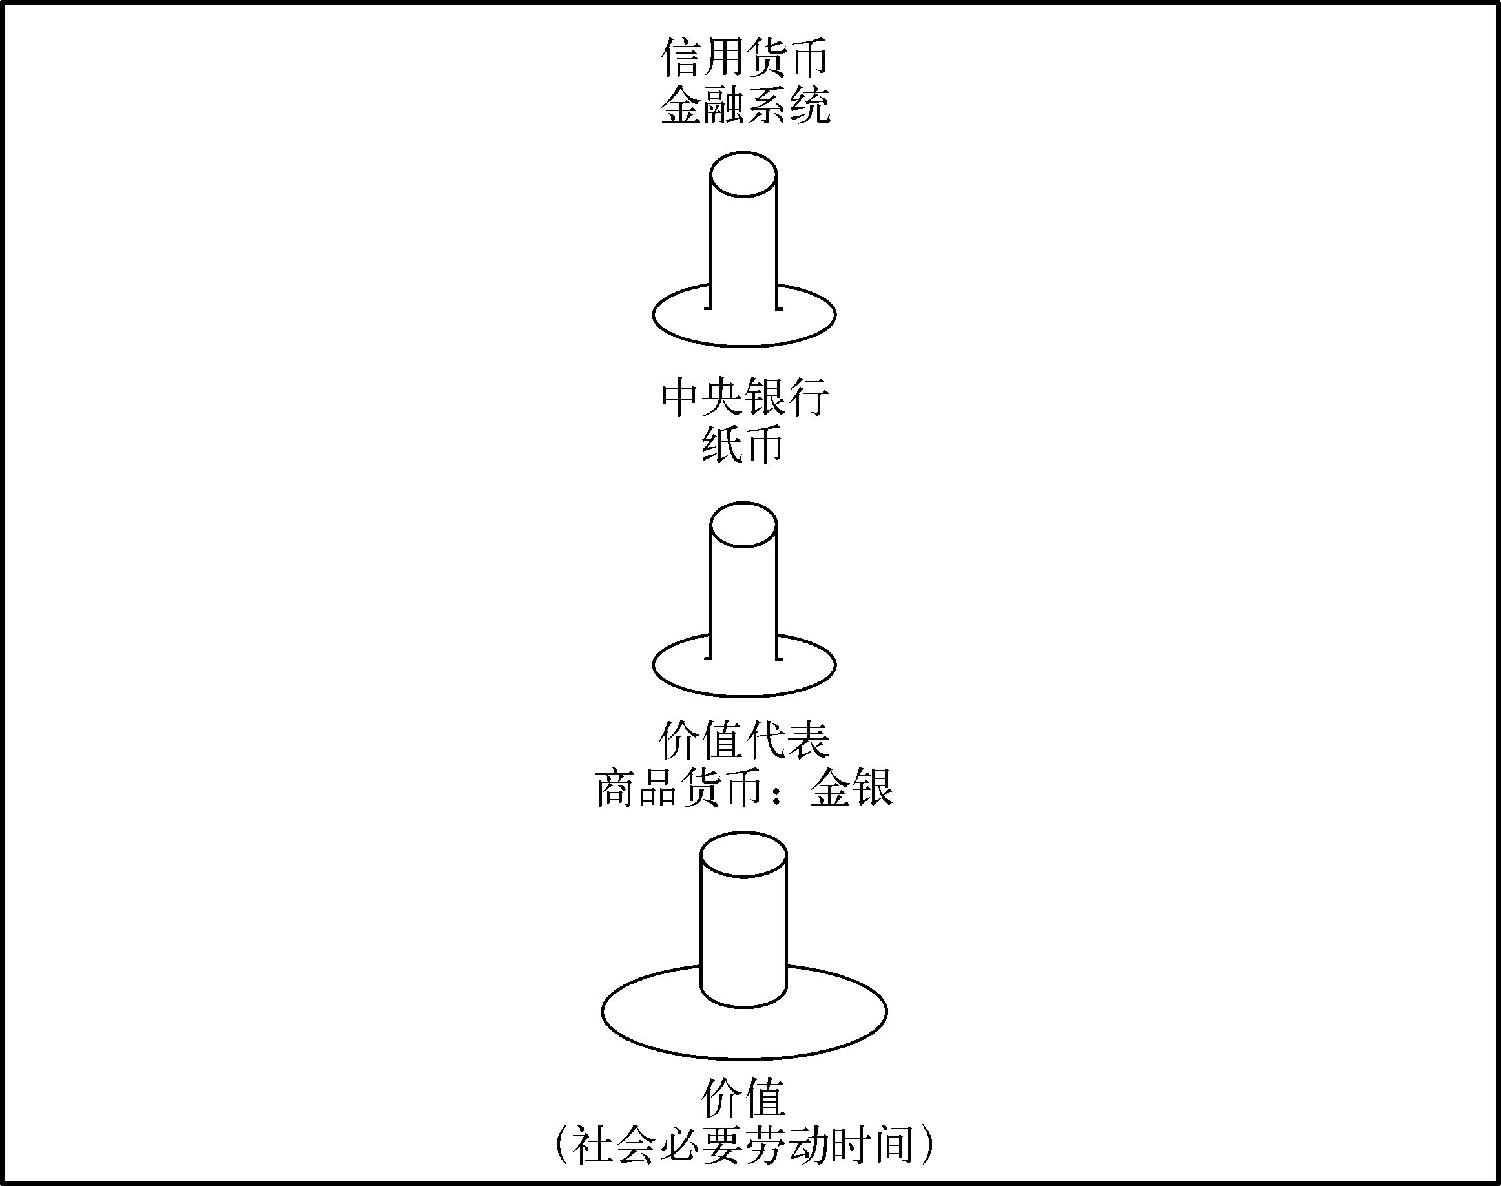
\includegraphics[scale=0.3]{david4.jpg}
\caption{马克思的等级制货币体系}
\label{fig:david4}
\end{figure}

尽管连全球信用和货币体系中徒有其表的金属或商品基础在20世纪70年代早期就被废除了
(虽然所谓的主张回归金本位的人还很多),全球金融体系枢纽(以美元为中心)的等级制
结构设想貌似依旧是合适的。我们比马克思活着的时候更接近这样一种现实:

\begin{quotation}
  同样作为财富的社会形式的信用,排挤货币,并篡夺它的位置。正是由于对生产社会性质
  的信任,才使得产品的货币形式表现为某种转瞬即逝的和观念的东西,表现为单纯想像的
  东西。

  但是,一当信用发生动摇,——而这个阶段总是必然地在现代产业周期中出现,——一切现实
  的财富就都会要求现实地、突然地转化为货币,转化为金和银。这是一种荒谬的要求,但
  是它必然会由这个制度本身产生出来。而应当能够满足这种巨大要求的全部金银,不过是
  银行地库里的几百万镑。\pagescite[][650]{capital3} (Big Big Note)

\end{quotation}

那么当信用货币和信用业务取代了商品货币之后会发生什么呢?第一,“在信用收缩或完全
停止的紧迫时期,货币会突然作为惟一的支付手段和真正的价值存在,绝对地同商品相对立。
因此,商品会全面跌价,并且难于甚至不可能转化为货币,就是说,难于甚至不可能转化为
它们自己的纯粹幻想的形式”。这里确切体现了拜物教理论。第二,“信用货币本身只有在
它的名义价值额上绝对代表现实货币时,才是货币”。当金流向国外时,信用兑换成货币的
可能性,即它和现实的金的同一性,就成问题了。为了保证这种兑换的条件,就采取各种强
制性的措施,提高利息率等等。……信用货币的贬值(更不用说它的只是幻想的货币资格的
丧失)会动摇一切现有的关系。因此,为了保证商品价值在货币上的幻想的、独立的存在,
就要牺牲商品的价值……因此,为了几百万货币,必须牺牲许多百万商品。这种现象在资本
主义生产中是不可避免的,并且是它的妙处之一……一旦劳动的社会性质表现为商品的货币
存在,从而表现为一个处于现实生产之外的东西,货币危机——与现实危机相独立的货币危机,
或作为现实危机尖锐化表现的货币危机——就是不可避免
的。\pagescite[][584-585]{capital3} (Big Big Note)

这就是20世纪30年代大萧条中发生的事情吗?这就是凯恩斯主义努力去纠正的“不可避免的”的问题吗?

\begin{quotation}
  这种情况之所以在资本主义体系内表现得最为尖锐,并且以矛盾百出、荒唐可笑的形式表
  现出来,是因为1. 在资本主义体系中,为直接的使用价值,为生产者本人的需要而进行的
  生产,已经完全废止,因此,财富只是作为社会过程而存在,这个社会过程表现为生产和
  流通的错综交织;2. 随着信用制度的发展,资本主义生产不断地企图突破对财富及其运动
  的这个金属的限制,\textbf{突破这个物质的同时又是幻想的限制,但又不断地在这个限制面前碰
  破头。}\pagescite[][650]{capital3}(Big Big Note)

\end{quotation}

马克思认为,纯粹基于商品货币的货币体系将会成为资本进一步积累的障碍,这是因为金的
数量满足不了需求。我们现在所谓的“金融抑制”是一个明显的、持续的危险,当货币(任
何种类)的数量不足以支撑资本积累带来的持续扩大的商品量流通时,这种“金融抑制”就
会出现。因此信用货币不但对资本主义的持续扩张是必需的,而且是至关重要的。有初步的
证据表明(虽然据我所知还没有经验研究)资本积累的历史是和信用货币的积累以及与其共
存的债务积累同步进行的。只有通过这种方式资本才能“\textbf{没有限制地}”进行积累。
但是如果资本积累取决于同时进行的信用货币和信用票据的积累,那么必定会产生一种基于
信念、信任和预期且会周期性突然失控的拜物教信仰。信用货币不是简单地代替贵金属货币:
他们会把货币体系和货币的概念带到一个全新的水平上,\textbf{会欢迎而不是揭穿在信用
  制度中所隐含的拜物教。}信用“泡沫”,资产泡沫,以及投机性的繁荣和萧条都是资本为
了将自己暂时地从货币—商品的限制中解放出来而必须付出的代价。(Big Big Note)

对信用制度至关重要的是,它具备冲破一切资本积累的货币障碍而无限制增长的能力。纸币
(欠条)的创造会导致无限制的可能性。美国2001年之后的房地产泡沫就是这样出现的。价
格在上升,每个人都从房价上涨中大赚一笔,而且他们赚得越多,价格就涨得越多。房子就
像ATM机一样,没有提取的限制,\textbf{直到人们意识到房地产的价格已经远远的超出了他们收入的
支付能力。}房地产市场的崩溃接踵而来。20世纪80年代日本的土地投机热潮破灭之后发生了
相同的事情。当崩溃来临时,所有者(掌控着硬通货)的资产流动性才是最重要的。当人们
发现\textbf{流动性不足的时候,止赎、损失和资产贬值就越积越多}。(Big Big Note)

但是,如果整个货币体系中的贵金属“枢纽”消失了,那么什么会取代它成为枢纽呢?答案
就是\textbf{世界央行和国家监管当局两者的结合体(我把它称作“国家—金融联合体”)},
它们共同形成了全球货币和信用制度的枢纽。对于马克思而言,这种枢纽就是英格兰银行,
而对我们而言,就是美国联邦储备银行(和美国财政部)和世界其他央行及监管当局,比如
英国、日本和欧盟的央行。然而\textbf{它们的效果是,用人造的制度取代依赖于实际商品
  生产(金和银)的调节机制。人们的判断是信用创造的唯一规则。}但是,人造的制度能正
确发挥作用吗?我们必须转而关注央行的组织和调节,以及政策是如何由国家机构制定出来
以应对信用制度的周期性过剩的。(Big Big Note)

现在人们普遍认为管制失灵影响了最近的几起事件,也有人鼓吹美国乃至全球经济危机的解
决之道就在于建立一个更好的监管机制。但是,我们应该如何利用这样的一个欧洲央行
呢?\textbf{它以控制通货膨胀为唯一目标而不顾失业,}它面对希腊债务危机时束手无策,
仅仅推行紧缩政策使得希腊元气大伤并日益衰退。人造的制度是不可靠的,受制于各种社会
势力和矛盾意见。他们创造了一个大不相同的调节机制,和商品货币依然作为枢纽时的央行
相去甚远。

即便在马克思的时代,金融机构及其政策的不可靠性也扮演了很重要的角色。马克思把“错
误的”1844年英国银行法案作为最好的例子。这项立法把英格兰银行分为了“一个发行部和
一个银行部”。[12]前一个部门持有政府债券和金属储备,以此为储备金发行银行券。该部
门用银行券(对贸易极为便利)换取金,并承诺如果需要的话,银行可以“支付给持券
者”金(在英国的银行券上,依旧可以找到答应支付给持券者的语句)。因此,在任何时候,
我拿着银行券去银行就可以换金。简而言之,银行券是可兑换的(停止兑现往往是那时候的
政治选择,实际上拿破仑战争期间英国就曾经中止兑现金)。另一个部门则贴现票据,承兑
支票,发行债券并参与其他传统的银行业务。1844年的立法在银行的两部分之间创造了一堵
防火墙。但是在1848年,一场信用危机打击了银行部。人们对已贴现商业票据和债券失去了
信心,发生了银行挤兑。银行部用光了金,而发行部门却拥有大量的金:

左拉的小说《金钱》以萨加尔(贝列拉兄弟)和甘德曼(罗斯柴尔德家族)在第二帝国时期的斗争为中心,描写金融投机中人们情感与理智的冲突。下面是萨加尔说的一番话,他想要说服他严肃、高尚、好沉思的侄女卡洛琳娜夫人,改变她瞧不起他的投机活动的想法:

\begin{quotation}
“看这儿,”萨加尔喊道,“你将会看到这些无人区和荒芜道路的彻底的复兴,我们的铁路将会穿过这些地方——是的!当我们把新的血液注入到这个体系的干涸的血管里时,土地将被清整,道路和运河将被建造起来,新的城市将会破土而出,生活也会好起来的。是的!这就是货币带来的奇迹……”

“你一定要明白,投机、赌博就是核心,是心脏。是的,它从各个小支流中吸引、收集了血液,然后再在河流中把血液输送到各个方向,于是\textbf{形成了一个巨大的货币流通},这正是大企业的生命所在。”

“投机——为什么是我们所必须经历的刺激物?因为投机是强迫我们生活、奋斗的永恒的欲望。没有了投机,噢我亲爱的朋友,什么类型的买卖都会没有……投机和爱情是一样的。相爱和投机都充满了肮脏;相爱时人们也仅仅考虑他们自己的喜悦;但是没有爱情就没有生命,那么世界就将终结。”
\end{quotation}

读了这段文字,你就可以很容易地理解,为什么马克思在提到贝列拉时会说起他“既是骗子又是预言家”。


信用制度看上去是混乱和不受约束的,它酝酿投机热潮和周期性崩溃的能力不受限制。这是可以预见的,因为利息,用《政治经济学批判大纲》里的话来说,属于特殊性,并且由其他特殊性调节(如果可能的话)——比如货币的供给和需求,还有不同资本派系之间的竞争。因此,利息注定是偶然、不受约束和失常的。利息也取决于信念。

对于这种阶级关系的永恒存在来说,资本“白手起家”的神话可以有效地巩固资产阶级在意识形态上的合法地位,同时使资产阶级得到更新和保持活力。因此缺乏向上的流动性(或是向上的流动性减小,正如美国近期那样)往往被看作是不利于维护资本主义社会秩序的。就现代信用制度促进了这种向上的流动性和灵活性来说,它也有积极的一面。(Note)

\begin{quotation}
这种反高利贷的激烈斗争,这种让生息资本从属于产业资本的要求,只是这样一种有机创造物的先声,这种有机创造物以现代银行制度为形式创造了资本主义生产的这些条件。现代银行制度,一方面把一切闲置的货币准备金集中起来,并把它投入货币市场,从而剥夺了高利贷资本的垄断,另一方面又建立信用货币,从而限制了贵金属本身的垄断。\pagescite[][682]{capital3} 

但是,绝不要忘记,第一,货币——贵金属形式的货币——仍然是基础,信用制度按其本性来说
永远不能脱离这个基础。第二,\textbf{信用制度以社会生产资料(以资本和土地所有权的
  形式)在私人手里的垄断为前提,}所以,一方面,它本身是资本主义生产方式固有的形式,
另一方面,它又是促使资本主义生产方式发展到它所能达到的最高和最后形式的动
力。\pagescite[][685]{capital3}

\end{quotation}

马克思显然把话说得太死了,因为我们现在的货币体系就不是以贵金属为基础的。我们也许
要用\textbf{怀疑的态度}来看待这个列宁一个世纪前提出的目的论观点,即\textbf{金融资
  本是资本主义生产方式可以采取的最高级也是最后的可能形式}。虽然毫无疑问金融资本在
一些历史阶段上变得更为突出,甚至拥有霸权地位,但是我认为资本各部分之间的力量均衡
不会注定只向一个方向演变的。(Big Note)

但是我们现在已经处于这样一个阶段,货币和国家之间的“内在关系”已经变得如此紧密,
以至于\textbf{很难想象一个可以从外部对金融化进行调控的国家力量}。证据便是美国最近
的多德—弗兰克金融管制改革法案。这个法案基本上是由银行家写的,不仅实施得不清不楚,
而且每条每款都主要遵循了银行业游说集团的意志。但是,如果我的观点——国家—金融联合体
在资本主义历史中发挥了长期的作用——是对的,那么这种“内在关系”不过是使资本回到了
它的起源。那么,这究竟是意味着国家仅仅是资本的一种工具,还是意味着近年来国家和金
融(注意,只是金融,而不是一般意义上的资本)的融合已经变形成了某种本质上完全不同
的东西?确实,债券持有人现在对国家政策的公开影响力似乎比以前更大了。但是我还记得
哈罗德·威尔逊(20世纪60年代的英国工党首相)曾经抱怨“苏黎世侏儒”决定其经济政策的
力量,正如他让步于伦敦金融家的需求而牺牲英国生产资本的利益一样。这和比尔·克林顿著
名的失意的感叹相同。在他的首次就职典礼前,克林顿对他的经济顾问们说:“你们的意思
是说,我的经济政策和连任前景都要取决于一群该死的证券交易员的观点?”对于这个问题,
答案是:“的确如此!”我认为,我们对国家和金融的力量交织历史的了解,还没有精细到
足以判断我们现在是否处在不同的处境的地步,尽管我们确定地知道金融管制和金融制度改
革的问题现在已成为了国际问题,任何一个国家都不可能单凭一己之力解决。

但是马克思特别讨论了信用制度内部的“内在力量”将把我们引向哪里。“资本的这种社会
性质,只是在信用制度和银行制度有了充分发展时才表现出来并完全实现。……因此,信用
制度和银行制度扬弃了资本的私人性质,从而自在地,但仅仅也是自在的包含着资本本身的
扬弃。”这是一个相当惊人的叙述,但是我们将会看到,马克思在其他地方会重复提
起。“银行业和信用同时又成了使资本主义生产超出它本身界限的最有力的手段,也是引起
危机和欺诈行为的一种最有效的工具。”

\begin{quotation}
毫无疑问,在由资本主义的生产方式向联合起来劳动的生产方式过渡时,信用制度会作为有力的杠杆发生作用;但是,它仅仅是和生产方式本身的其他重大的有机变革相联系的一个要素。与此相反,关于信用制度和银行制度的奇迹般的力量的种种幻想所以会被赋予社会主义的意义,是由于对资本主义生产方式和作为它的形式之一的信用制度完全没有认识。\pagescite[][686]{capital3} 
\end{quotation}

\chapter{信用和银行系统的作用(第三卷 第27章开始)}

第27章,马克思列举了许多金融部门发挥的重要作用。总结如下:

1. 它促进了货币资本在部门和产业之间的顺畅流动,这样利润率到处都被平均化了。马克思
在此之前把信用的功能归为“阶级的共有资本”,我认为主要就是这个意思。资本的“蝴
蝶”形式不停地移动,使不同产业、活动和地区的收益率标准化。

2. 它显著地减少了(a) 流通费用——通过免除商品货币的使用,用纸币取代黄金和降低了为适应商品交换的波动而持有准备金(窖藏)的必要性,同时(b) 减少周转时间(或者“加速商品形态变化的速度”和加速“货币流通的速度”)。这种流通的加速通常会延伸到资本的再生产过程。总之,它促进了资本的加速(周转时间的分析很清楚地表明了这点)。

3. 它允许股份公司的成立,使可能的生产规模惊人地扩大了,允许以前的政府职能私有化,
并有助于集中资本(正如第一卷中提到的)。这意味着许多资本主义企业现在取得了和私有、
个人相对立的社会特征。马克思有些令人惊讶地推断:\textbf{“这是作为私人财产的资本
  在资本主义生产方式本身范围内的扬弃。”}它加强了这种转化——“实际执行职能的资本家
转化为单纯的经理,别人的资本的管理人,而资本所有者则转化为单纯的所有者,单纯的货
币资本家。”\pagescite[][495]{capital3}

\begin{quotation}
因为利润在这里纯粹采取利息的形式,所以那些仅仅提供利息的企业仍然可以存在;这是阻止一般利润率下降的原因之一,因为这些不变资本比可变资本庞大得多的企业,不一定参加一般利润率的平均化。\pagescite[][496]{capital3} (Big Note)

\end{quotation}

保罗·博卡拉(Paul Boccara),20世纪60年代末法国共产党的主要理论家,认为这是这些年
中阻碍利润率趋于下降的主要力量。\textbf{投资于大规模基础设施的资本(不论是由国家还是股份
公司融资)的确可以,而且一般也是以这种方式流通的——只要求利息,事实上补贴了其他地
方的利润。个别资本家也可以选择租用他们的大部分不变资本(比如叉式升降车和其他形式
的机械),从而节约了大量不变资本的费用(对他们而言)。他们只支付了以商品形式借贷
的资本的等值利息,而不是支付商品的全部价值(利息加利润)。} (Big Big Note)

现在,固定资本的物理量(physical mass)嵌入建成环境(这个物理量证明了生产中不变资
本与可变资本比率极大提高的观点)中,\textbf{这种固定资本的绝大部分主要不是通过相关商品的
直接买卖而是作为获取租金的生息资本进行循环。地租的榨取和生息资本流通(巨额的抵押
贷款市场的存在就是绝好的例证)之间的关系就成为资本主义动态中的重要特征。}这是一个
马克思几乎没有涉及的话题(尽管我们很快就会看到,抵押贷款被定义为“虚拟资本”的一
种形式)。(Big Big Note: 我们国家的城镇化策略是不是也这样呢?)

\begin{quotation}


它在一定部门中造成了垄断,因而引起国家的干涉。它再生产出了一种新的金融贵族,一种新的寄生虫,——发起人、创业人和徒有其名的董事;并在创立公司、发行股票和进行股票交易方面再生产出了一整套投机和欺诈活动。这是一种没有私有财产控制的私人生产。\pagescite[][497]{capital3} 

\end{quotation}
第二帝国时期巴黎风趣的评论者们说,资本和商业变成了“其他人的钱”,指的就是这种情况。这就是贝列拉兄弟构想的世界:圣西门的乌托邦成为反乌托邦。马克思指出的“金融贵族”在今天更加显要。

“信用为单个资本家或被当作资本家的人,提供在一定界限内绝对支配他人的资本,他人的
财产,从而他人的劳动的权利……对社会资本而不是对自己的资本的支配权,使他取得了对
社会劳动的支配权。”马克思认为这里涉及的社会化有巨大的潜在重要性。“一个人实际拥
有的或公众认为他拥有的资本本身,只是成为信用这个上层建筑的基础。”结果,“在这里,
一切尺度,一切在资本主义生产方式内多少还可以站得住脚的辩护理由都消失了。进行投机
的批发商人是拿社会的财产,而不是拿自己的财产来进行冒险的。资本起源于节约的说法,
也变成荒唐的了,因为那种人正是要求别人为他而节约”。\pagescite[][498]{capital3} (Big Big Note)

\begin{quotation}
在资本主义生产很不发达的阶段还有某种意义的各种观念,在这里变得完全没有意义了。在这里,成功和失败同时导致资本的集中,从而导致最大规模的剥夺。在这里,剥夺已经从直接生产者扩展到中小资本家自身。这种剥夺是资本主义生产方式的出发点;实行这种剥夺是资本主义生产方式的目的,而且最后是要剥夺一切个人的生产资料……这种剥夺在资本主义制度本身内,以对立的形态表现出来,即社会财产为少数人所占有;而信用使这少数人越来越具有纯粹冒险家的性质。因为财产在这里是以股票的形式存在的,所以它的运动和转移就纯粹变成了交易所赌博的结果;在这种赌博中,小鱼为鲨鱼所吞掉,羊为交易所的狼所吞掉。\pagescite[][498]{capital3} (Big Big Note)

\end{quotation}

他考察货币经营资本历史时要阐明的一般主题是,高利贷和利息必须被规训并服从于一般的
资本主义生产方式以及特殊的产业资本循环的要求。然而这些段落意味着资本主义信用制度
完全不受控制,以致它现在反而以有害的、扭曲的方式威胁到资本和剩余价值生产的世界。
它以掠夺式积累而不是在生产领域剥削劳动力为中心。它在经济中再次引入高利贷业务,尽
管和很久以前的高利贷完全不同。这会威胁到资本积累的持续性吗?马克思没有给出明确的
答案,但确实暗示了这种可能性。

\begin{quotation}


信用制度是资本主义的私人企业逐渐转化为资本主义的股份公司的主要基础,同样,它又是按或大或小的国家规模逐渐扩大合作企业的手段。资本主义的股份企业,也和合作工厂一样,应当被看作是由资本主义生产方式转化为联合的生产方式的过渡形式,只不过在前者那里,对立是消极地扬弃的,而在后者那里,对立是积极地扬弃的。\pagescite[][499]{capital3} 

\end{quotation}
马克思完成这一章的草稿后,恩格斯插入了几页来描述公司资本的力量的演化。可以推断出,恩格斯认为从这一切中建立任何进步事物的时机都早已过去了。恩格斯在其他地方写到,马克思非常尊敬圣西门的思想,即为了进步的目的运用联合起来的资本的力量。在这里,马克思美化了这个思想,并提出了通过工人的协同控制来管理联合起来的资本的前景。尽管他承认这些工人合作社注定会再生产出现存制度的许多缺点,但它们至少为通过合作运动和实践的传播来征服一个国家提供了一个依据。(Big Note)

这一问题很重要,因为当代许多正在进行的运动相信这一时机已经再次来临了——通过接管工
厂进行的生产的民主化,可选择的“团结经济”(Solidarity Economy)的发展,物物交换
网络和其他合作形式——它们本身就是一条通向一个彻底反资本主义的政治和经济生活重建的
道路。尽管许多参与者意识到,在合作社形式里,不仅自我剥削十分困难,而且不可避免地
再生产出了他们寻求取代的资本主义制度的很多缺陷,这条道路还是经常被描述为民主的反
资本主义运动的唯一选择。似乎信用制度的兴起和资本社会化提供了合作社和工人控制可能
兴盛的“自然”基础。然而,这里没有提到《共产党宣言》中把所有信用集中于工人控制的
国家手中的要求。

但是也有许多引人警戒的故事。前些年,皮奥里和萨贝尔写了一本颇有影响力的《第二次产
业革命》。他们提出,弹性专业化和小批量生产的新劳动实践,为工人控制的小规模合作生
产(如第三意大利的艾米利亚—罗马涅区所展示的)开辟了空间(和1848年存在的相似);这
种形式将打败公司主导的工厂生产形式,并提供转化到分散的社会主义的机制。[15]皮奥里
和萨贝尔发起了一场相当有效的运动(特别是在欧洲)来说服组织起来的工人放弃对新技术
和新组织形式的敌意,让他们像拥护自由解放一样拥护弹性专业化(他们非常迷恋蒲鲁东的
观点,当然这些观点是马克思不能容忍的)。皮奥里和萨贝尔没有意识到的是,弹性专业化
促进了灵活积累下的恶意剥削的实践,而灵活积累居于新自由主义计划的核心。弹性专业化
成为所有采用它的生产场所中规训和压制劳动力的主要手段。现在再没人亲切地说它能带来
解放了。\textbf{历史上很多事物看似蕴含着解放的可能性,结果却是资本主义剥削的支配性实践的
回归,这的确很令人悲哀。所以,当心你自己的愿望。}

从马克思的角度来看,更有意义的区别是货币被资本家用来购买用于生产的商品,还是被借来购买已经生产出来的商品。这个区别是“收入的货币形式和资本的货币形式之间的区别”。\pagescite[][503]{capital3} 两种货币的使用都包含在产业资本的流通中。马克思有时把流入生产的信用称为“货币资本”,与流向消费者支持市场中价值和剩余价值实现的“货币经营资本”相对立。

马克思仔细考察了当银行资本为了利息的回报而借出时会发生什么。他指出,利息可以看作
是任何收入流的等价物。如果利率是5\% ,那么“每一笔固定的二十五镑的年收入,都可以
看作五百镑资本的利息”。但马克思评论这是一种“纯粹幻想的观念”。收入流的后面不一
定要有任何实际的货币资本。比如,许多美国公民每月都会收到社会保险支票,但认为这笔
货币流是某些国家持有的资本的利息的想法是一种幻觉。然而,社会保险接受者如果承诺把
每年收到的二万五千美元交给银行,就可以获得五十万美元的货币资本来买房子。二万五千
美元的年收入被资本化为五十万美元,\textbf{即使社会保险金后面没有初始的货币资本量
  (只是国家提供每月收入的一种承诺,它以对工资征税的方式获得资金)。}这使我们考虑
马克思最重要的概念之一,虚拟资本。

\begin{quotation}
  但在这一切场合,这种资本,即把国家付款看成是自己的幼仔(利息)的资本,
  是\textbf{幻想的虚拟的资本}。…… 这个金额从来不是要作为资本支出的,不是要作为
  资本投下的,而只有作为资本投下,它才能转化为一个自行保存的价值。……不管这种交
  易反复进行多少次,国债的资本仍然是纯粹的虚拟资本;一旦债券不能卖出,这个资本的
  假象就会消失。然而,我们马上就会知道,这种虚拟资本有它的独特的运
  动。\pagescite[][527]{capital3}

生息资本一般是一切颠倒错乱形式之母。……资本家们思考方式的错乱在这里达到了顶点,资本的增殖不是用劳动力的被剥削来说明,相反,劳动力的生产性质却用劳动力本身是这样一种神秘的东西即生息资本来说明。\pagescite[][528]{capital3} 
\end{quotation}

马克思提到的“独特的运动”是那种我们看到的股票和债券市场每天甚至每小时的价值波动。
当资产阶级理论家把工资流归于劳动者并且创造出物化在工人身上的虚拟资本时,这种颠倒
错乱更显著地表现出来了。工人的价值就被计算为年工资的资本化价值。所以根据这个理论,
如果工人投资教育和获得技能,人力资本价值就可以提高,他将以更高工资的形式得到回报。
按照人力资本理论,工人是资本家!

所有这些背后有一个简单却关键的原则,即资本化:“人们把虚拟资本的形式叫作资本化。
人们把每一个有规则的会反复取得的收入按平均利息率来计算,把它算作是按这个利息率贷
出的一个资本会提供的收益。”这笔收益流的所有权证书可以按照这个资本化的价格交
易。“因此,和资本的现实增殖过程的一切联系就彻底消灭干净了。资本是一个\textbf{自
  行增殖的自动机}的观念就牢固地树立起来了”。

\begin{quotation}
  即使在债券——有价证券——不像国债那样代表纯粹幻想的资本的地方,这种证券的资本价值
  也纯粹是幻想的。我们上面已经讲过,信用制度怎样产生出联合的资本。这种证券被当作
  代表这种资本的所有权证书。铁路、采矿、轮船等公司的股票代表现实资本,也就是代表
  在这些企业中投入的并执行职能的资本,或者说,代表股东所预付的、在这些企业中作为
  资本来用的货币额。这里决不排除股票也只是一种欺诈的东西。但是,这个资本不能
  有\textbf{双重存在}:一次是作为所有权证书即股票的资本价值,另一次是作为在这些企
  业中实际已经投入或将要投入的资本。它只存在于后一种形式,股票不过是对这个资本所
  实现的剩余价值的一个相应部分的所有权证书。

  这些所有权证书的价值的独立运动,加深了这样一种假象,好像除了它们能够有权索取的
  资本或权益之外,它们还形成现实资本……这种证券的市场价值部分地有投机的性质,因
  为它不是由现实的收入决定的,而是由预期得到的、预先计算的收入决定
  的。 \pagescite[][529-530]{capital3}

\end{quotation}
事实上,它是对可能产生剩余价值的未来劳动的索取权,其中的一部分是利息(对纯粹的所有权的回报)。

危机中财富和权力加速集中是一个重要的历史事实(2007—2012年的金融危机证实了这点)。(Big Big Note)

\begin{quotation}
银行家资本的最大部分纯粹是虚拟的,是由债权(汇票),国债券(它代表过去的资本)和股票(对未来收益的支取凭证)构成的。在这里,不要忘记,银行家保险箱内的这些证券,即使是对收益的可靠支取凭证(例如国债券),或者是现实资本的所有权证书(例如股票),它们所代表的资本的货币价值也完全是虚拟的,是不以它们至少部分地代表的现实资本的价值为转移的;既然它们只是代表取得收益的要求权,并不是代表资本,那么,取得同一收益的要求权就会表现在不断变动的虚拟货币资本上。此外,还要加上这种情况:这种虚拟的银行家资本,大部分并不是代表他自己的资本,而是代表公众在他那里存入的资本——不论有利息,或者没有利息。\pagescite[][532]{capital3} (Note)

\end{quotation}


我认为,这是马克思将信用制度解释为“自主的”和“独立的”但仍包含在资本运动的一般
规律之中的理由。…… 我最喜欢的类比是它有点像青少年:一方面他们永远要求并声明他们
独立和自主的权利,同时另一方面,他们的资金和法律保障锚定在家里,所以当事情出问题
时他们就跑回家找妈妈和爸爸。某种程度上这看起来是一种恰当的类比,这是货币和信用制
度发挥作用的总体方式,每一层枢纽都由永远喧闹的青少年构成,而顶层运行的“宇宙之
王”则最为混乱(见图\ref{fig:david4})。当体系坠毁时,他们都冲回到家中去找父母般
的政府,希望得到救助,而政府作为一位宽容慈爱的家长,总是会救助他们。(Big Big
Note)

但是,尤其是在危机时期,似乎有某种位于价值关系世界中的规训力量,\textbf{恢复了体
  系的秩序。}然而,马克思也承认,信用制度内的信任危机和预期危机,会对价值和剩余价
值生产造成严重破坏。


\begin{figure}
\centering
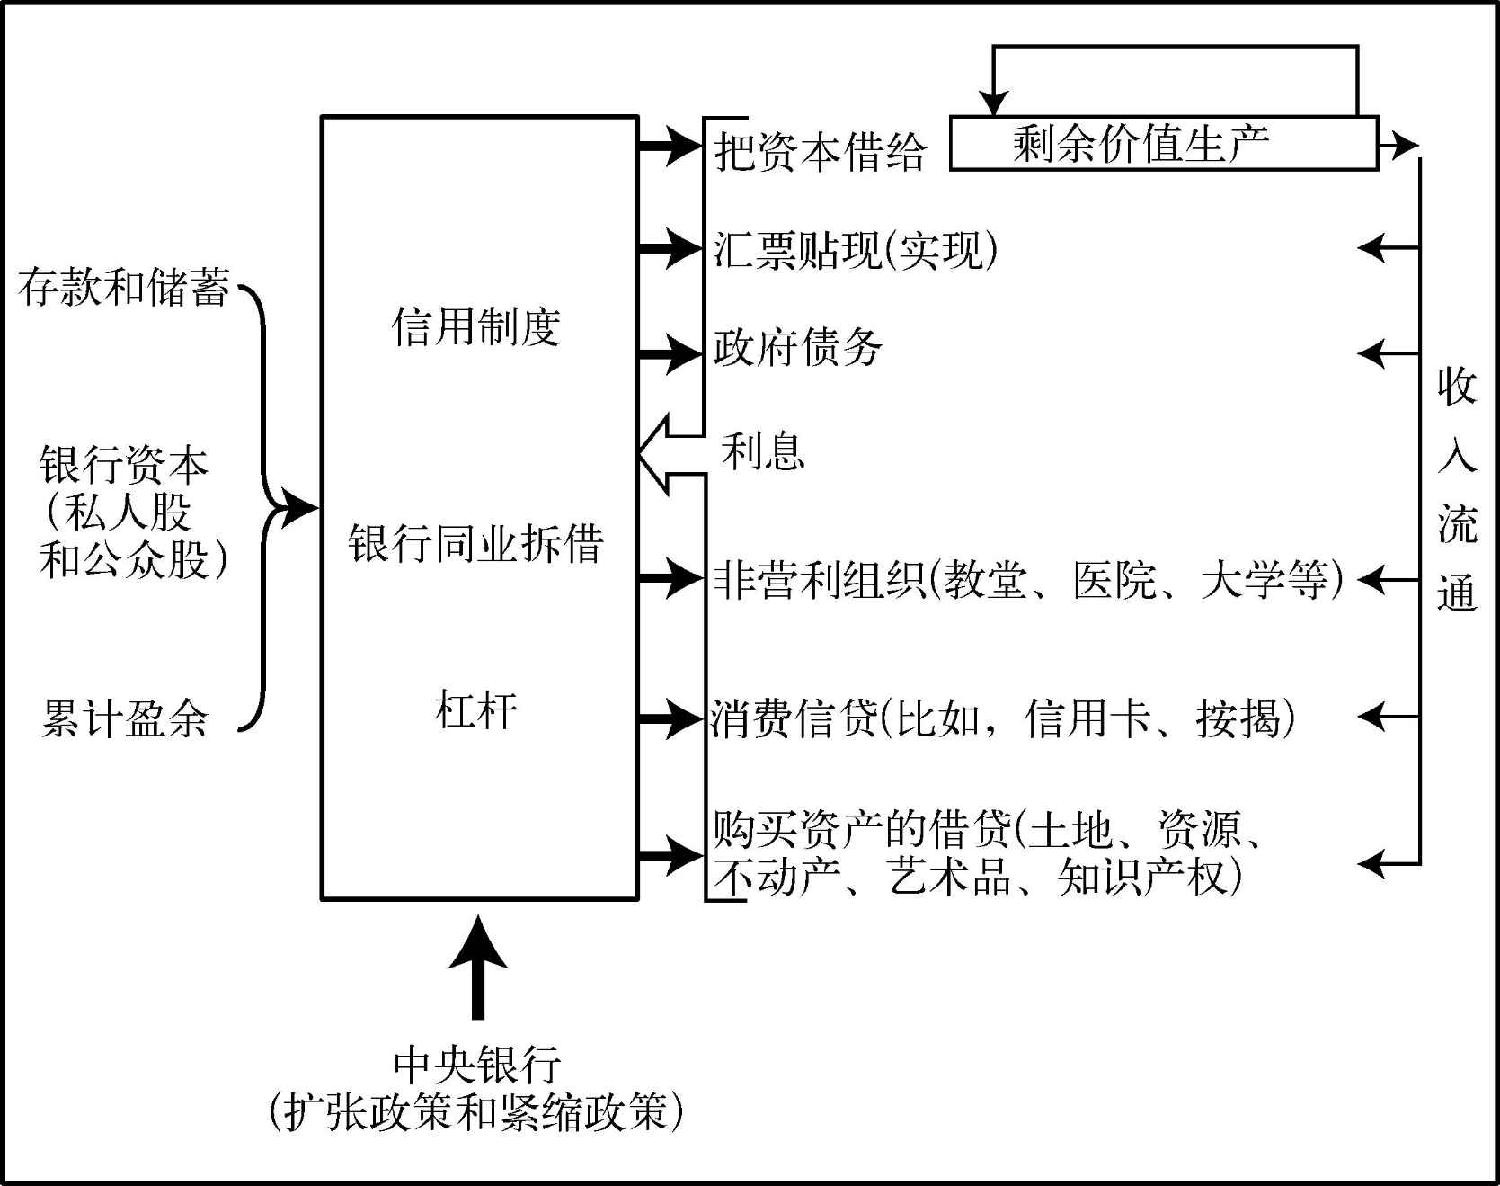
\includegraphics[scale=0.3]{david5.jpg}
\caption{生息资本的横向流通}
\label{fig:david5}
\end{figure}

货币借出的形式:
\begin{enumerate}
\item 借贷资本

  货币借给生产者,用来购买从事剩余价值生产所需要的不变资本和可变资本。……这些借
  出的货币用来进行实际的价值和剩余价值生产。其中没有任何虚拟的东西(尽管所有这种
  投资从定义来说无疑都具有投机性)。然而,当货币以发行股票的方式取得时,事情看起
  来有些不同。股票实际上是一种附属于纯粹的货币所有权的财产权。它实际上是对未来剩
  余价值生产的一个份额的法定索取权。

股票与证券是一种虚拟资本的形式,但是它们的虚拟特征因为与价值和剩余价值生产依然保持的宽松联系而得到缓解(用货币术语来说,企业收益支撑了股票价值)。然而,像安然那样的公司,虽然股票价格很高,并没有剩余价值被实际生产出来。它公布的收益是欺骗性的。

\item 用于价值实现的借贷

  货币可以被借出去实现已经生产出的商品的价值(甚至是还没生产出的,正如还没收割的农作物或将要建的房屋)。贴现率等同于那些将来某天到期的汇票的利息率。

 \item 政府借贷和国债

   政府可以凭借它获取收入(通过税费)的能力借到资本。它承诺将预期未来收益的一部分
   作为一笔资本的回报。政府债务的证书在借到的货币花光很久以后都能交易。大部分政府
   花费的货币与剩余价值生产几乎没有或完全没有直接的关系(尽管它经常通过形成一个可
   行的市场而发展出间接的关系,比如,军事装备)。这是\textbf{最卓越的虚拟资本}。
   政府一般不生产价值或剩余价值(例如,它维持君主制和打仗)。收入税被转化为源源不
   断的利息支付,它可以被资本化为一个总额,从而作为对未来收入的索取权进行交易。政
   府支出的一些类别确实和剩余价值生产相关。存在政府运营的企业(这些企业在世界许多
   地方都很重要,直到大约1980年后的新自由主义私有化浪潮的兴起,但它们在中国仍然很
   重要)。尽管这些企业不一定要获得利润,但它们以更低的成本向其他企业提供投入,这
   影响了整体的利润率。政府也投资于生产所必需的基础设施建设(高速公路、公共设施、
   排污和供水等等)。\textbf{它可以提供这些不变资本投入,只要求利息作为回报,因此
     有助于缓解任何利润率下降的趋势。}比如,债务融资的“生产性政府支出”这个范畴
   早在豪斯曼男爵重建第二帝国巴黎的基础设施时就变得极为重要了。但是大多数的政府债
   务是纯粹虚拟的。(Big Note)

\item 非营利组织的借贷

  包括私立医院、大学、教堂、博物馆和各类文化机构。对它们的借贷属于\textbf{虚拟资
    本的范畴,}因为他们多半不生产价值或剩余价值(尽管一些大学和医院的分支机构通过
  创新和研究直接涉及剩余价值生产)。用于支付借贷利息的收入有各种来源,但在我们的
  时代主要是依靠\textbf{使用费和捐赠}。

  \item 消费者信贷

    迄今为止,美国最重要的消费者信贷形式是房地产抵押贷款,马克思明确将其列为虚拟
    资本形式的一种。尽管家中没有发生直接的价值或剩余价值生产,家务劳动在确定劳动
    力价值方面的作用显著影响了剩余价值的生产。消费者信贷现在蕴藏着巨大的商机,它
    在管理经济中的总需求和为“\textbf{第二级的剥削形式}”提供充足机会中起了关键作
    用。马克思偶尔承认这种“第二级的剥削形式”,但一般将其作为边缘形式而不考虑。(Note)
   \item 为了取得和购买资产及其他索取收入的纸质证书而进行的借贷(比如自然资源的特许权、专利、土地和房产的租金)

\end{enumerate}

\bigskip
资产市场(从艺术投资到土地和资源买卖的所有事物)的扩散已经成为近来资本主义历史上的显著特征。大量过剩的货币经营资本涌向这些市场。


银行家一般不歧视(尽管他们可能会专门化)这些不同的借贷选择。他们的资本会流向任何
需求、回报率和安全性最有利的地方,以及任何未来前景看起来最光明的地方。\textbf{预
  期}——对未来的信念——在这些市场的运转中发挥了主导性作用。也存在这种可能,即一些投
资可能性被其他需求(和预期)更高的投资所“\textbf{挤出}”。(这是常见的对大规模政
府借贷或资产泡沫的批评:\textbf{它们挤出了对生产性活动的投资并增加了其他投资活动
  的利息成本。})(Big Note: 不理解这句话)

在生息货币资本的流动中,不平衡会频繁发生。恰恰因为这些资本是独立的、自主的,它们
可以影响总体的资本主义发展的运动规律,同时自己周期性地单独酝酿一场危机。例如,如
果大量过剩的货币经营资本流入土地和房地产市场(正如发生在20世纪80年代的日本以
及2000年后的美国、西班牙、爱尔兰等国的情况),那么,就会造成信用流通的巨大扭曲和
资产价值的投机性繁荣,直到崩溃发生并进行强制纠正。(Big Note)

即使在泡沫状况还不明显的时候,美国采取了许多措施把信用扩张到房屋所有权。这是资本从一般消费者,特别是从劳动者那里重获财富的主要方式。(Big Note)

\begin{quotation}
  资本的现实积累的标志,即规模扩大的再生产的标志,又在什么程度上不是这种标志呢?
  所谓资本过剩(plethora),一个始终只用于生息资本即货币资本的用语,仅仅是表现产
  业生产过剩的一个特殊方式呢,还是除此以外形成的一种特殊的现象呢?这种过剩即货币
  资本的供给过剩,是否与停滞的货币总量(金银条块、金币和银行券)的存在相一致,从
  而现实货币的这种过剩,是否就是借贷资本的上述过剩的反映和表现形式
  呢?

货币紧迫,即借贷资本不足,又在什么程度上反映出现实资本(商品资本和生产资本)的不
足呢?另一方面,它又在什么程度上与货币本身的不足,即流通手段的不足相一致呢?\pagescite[][539]{capital3}
\end{quotation}

再一次用当代的说法,货币供给收缩和银行间信贷的冻结是由中央银行和国家权力机关施加的金融收缩的信号吗?还是缺乏有利可图的投资机会的信号?(Big Note)

这背后有一个更一般的问题:债务的积累和财富的积累在什么程度上是有关联的?这是虚拟
资本形式的增殖所提出的问题。比如,“国债资本的积累,不过是表明国家债权人阶级的增
加,这个阶级有权把税收中的一定数额预先划归自己所有”。因此,“连债务积累也能表现
为资本积累”。\pagescite[][540]{capital3} 但是,像往常一样,“表现”这个词标志着
在拜物教面具的背后很可能有别的事情正在发生。发生了什么呢?问题是国债(虚拟资本)
积累可以转化为实际的货币资本,从而使虚拟资本变成现实资本。但这假定了国债是可以交
易的。这反过来意味着虚拟资本继续和以前一样流通。股票和有价证券也是如此,它们
是“不存在的资本的名义代表”:

\begin{quotation}
当这些证券的积累表示铁路、矿山、汽船等等的积累时,它们也表示现实再生产过程的扩大,就像动产征税单的扩大表示这种动产的增加一样。但是,作为纸制复本,这些证券只是幻想的,它们的价值额的涨落,和它们有权代表的现实资本的价值变动完全无关,尽管它们可以作为商品来买卖,因而可以作为资本价值来流通。\pagescite[][540-541]{capital3} 

\end{quotation}

当按揭贷款打包成为债务抵押债券时,它们似乎以过去的两倍的虚拟状态存在;但是当对冲基金经理把它们卖给毫不怀疑的、轻信的投资者并出色地赚了十亿时,很遗憾,他获得了一点都不虚幻的实际货币权力。


\begin{quotation}
  由这种所有权证书的价格变动而造成的盈亏,以及这种证书在铁路大王等人手里的集中,
  就其本质来说,越来越成为赌博的结果。赌博已经取代劳动,表现为夺取资本财产的本来
  的方法,并且也取代了直接的暴力……这种想象的货币财产,不仅构成私人货币财产的很
  大的部分,并且正如我们讲过的,也构成银行家资本的很大的部分。(Big Big Note)

  ……整个信用制度的惊人的扩大,总之,全部信用,都被他们当作自己的私有资本来利用。
  这些人总是以货币的形式或对货币的直接索取权的形式占有资本和收入。这类人的财产的
  积累,可以按极不同于现实积累的方向进行,但是无论如何都证明,他们攫取了现实积累
  的很大一部分。\pagescite[][541]{capital3}

  只要再生产过程顺畅地进行,从而资本回流确有保障,这种信用就会持续下去和扩大起来,
  并且它的扩大是以再生产过程本身的扩大为基础的。一旦由于回流延迟,市场商品过剩,
  价格下降而出现停滞,产业资本就会过剩,不过这种过剩是在产业资本不能执行自己的各
  种职能的形式上表现出来的。有大量的商品资本,但卖不出去。有大量的固定资本,但由
  于再生产停滞,大部分闲置不用。(Note: 马克思对周期的一个描述)\pagescite[][546-547]{capital3} 

  一旦新的危机爆发,信用突然停止,支付停滞,再生产过程瘫痪……在借贷资本几乎绝对
  缺乏的同时,闲置的产业资本发生过剩。
\end{quotation}

借贷资本的积累可以从正常资本的积累中“沉淀下来”。“在现实积累不断扩大时,货币资
本积累的这种扩大,一部分是这种现实积累扩大的结果,一部分是各种和现实积累的扩大相
伴随但和它完全不同的要素造成的结果” ——比如,生产性公司的股票和证券价值上升——“一
部分甚至是现实积累停滞的结果”——过剩商品没有卖出去,但是它的贴现价值通过汇票实现
了。但“这种积累可以表示各种和现实积累很不相同的要素”——比如,资本化后上升的资产
价值、政府虚拟资本的形成或消费信贷。总结果就是“在周期的一定阶段出现货币资本的过
剩”。\pagescite[][574]{capital3}

随后信用就收缩,“(1) 因为这种资本闲置不用;(2) 因为再生产过程顺畅进行的信念已经遭到破坏;(3) 因为对这种商业信用的需求已经减少。”[43]信用的缺乏使得

\begin{quotation}
  通过信用来获得商品就比较困难……在危机中,因为每个人都要卖而卖不出去,但是为了
  支付,又必须卖出去,所以,正是在这个信用最缺乏的时刻,不是闲置的寻找出路的资本,
  而是停滞在自身的再生产过程内的资本的数量最大。这时,由于再生产过程的停滞,已经
  投入的资本实际上大量地闲置不用。工厂停工,原料堆积,制成的产品作为商品充斥市场。
  因此,如果把这种情况归因于生产资本的缺乏,那就大错特错了。正好在这个时候,生产
  资本是过剩了,无论就正常的、但是暂时紧缩的再生产规模来说,还是就已经萎缩的消费
  来说,都是如此。\pagescite[][574]{capital3}

\end{quotation}

“我们假定整个社会只是由产业资本家和雇佣工人构成”——撇开其他所有特征,比如价格波
动和信用制度所助长的买空卖空和投机交易。这样,

\begin{quotation}
  危机好像只能由各个不同部门生产的不平衡,由资本家自己的消费和他们的积累之间的不
  平衡来说明。然而实际情况是,投在生产上的资本的补偿,在很大程度上依赖于非生产阶
  级的消费能力;而工人的消费能力一方面受工资规律的限制,另一方面受以下事实的限制,
  就是他们只有在他们能够为资本家阶级带来利润时才能被雇佣。\textbf{一切现实的危机
    的最后原因,总是群众的贫困和他们的消费受到限制,而与此相对比的是,资本主义生
    产竭力发展生产力,好像只有社会的绝对的消费能力才是生产力发展的界
    限}。\pagescite[][574-578]{capital3}(Big Big Note)


\end{quotation}

这当然是最有名的论断之一(第二卷第351页也有),\textbf{和利润率下降是“现代政治经
  济学最重要的规律”这一断言一样,也需要结合上下文语境来理解。}对产业周期的研究表
明,这两种陈述之间并没有必然的对立。由于群众消费受到限制,利润率在短期内可能会下
降。这和第三卷前面章节中通常用来解释利润率下降的机制是非常不同的。但是解雇工人会
减少市场需求,使得商品卖不出去和生产能力闲置,从而诱发资本家减少工资并解雇更多的
工人。马克思清楚地看到了产业周期中这种螺旋式下跌的可能性。这是否形成了一个长期趋
势完全是另一个问题。信用制度允许资本摆脱这种直接的消费限制,至少在一段时间内是这
样的。“信用的最大限度,等于产业资本的最充分的运用……不顾消费界限”。在大
约1980年以后的工资压制的新自由主义时期,私人消费主要是通过扩展消费信贷来维持的。

马克思也观察到这种螺旋式下降在信用的帮助下如何可能\textbf{反转}过来。大量的闲置借
贷和货币资本——伴随着低利率——在危机后形成,并成为复苏的关键。“在危机以后的复苏时
期,人们要求借贷资本,却是为了购买,为了把货币资本转化为生产资本或商业资本。所以,
这时,要求借贷资本的,或者是产业资本家,或者是商人,产业资本家把借贷资本用于购买
生产资料和劳动力。”\pagescite[][580]{capital3} \textbf{低利率使对固定资本的长期
  投资和开启全新的事业看上去更有吸引力。}\pagescite[][553]{capital3} 在扩张的初始
阶段利率通常维持在较低水平,这时宽松信贷发挥着其最具有建设性的作用,而这有助于进
一步的扩张和世界市场的一体化,正如我们所见的。(Big Note: 当前的中国,是否是低利
息率呢?)
在他第一次试图解释周期性运动如何开展时,马克思写道:

\begin{quotation}
  如果再生产过程再一次达到过度紧张状态以前的那种繁荣局面,商业信用就会大大扩张,
  这种扩张实际上又是资本容易流回和生产扩大的“健全”基础。在这种情况下,利息率虽
  然已经高于最低限度,但是仍然很低……由于资本回流容易并且具有规则性,加上商业信
  用扩大,这就保证了借贷资本的供给(虽然需求已经增长),防止了利息率水平的上升。
  另一方面,只有到这时,没有准备资本甚至根本没有任何资本而完全依靠货币信用进行操
  作的冒险家们,才引人注目地涌现出来。此外,还有各种形式的固定资本的显著扩大和新
  型大企业的大批开张。现在,利息提高到它的平均水平。一旦新的危机爆发,信用突然停
  止,支付停滞,再生产过程瘫痪……在借贷资本几乎绝对缺乏的同时,闲置的产业资本发
  生过剩……这种产业周期的情况是,同样的循环一旦受到最初的推动,就必然会周期地再
  现出来。\pagescite[][553-554]{capital3} 

  
  在再生产过程的全部联系都是以信用为基础的生产制度中,只要信用突然停止,只有现金
  支付才有效,危机显然就会发生,对支付手段的激烈追求必然会出现。所以乍看起来,好
  像整个危机只表现为信用危机和货币危机。而且,事实上问题只是在于汇票能否兑换为货
  币。但是这种汇票多数是代表现实买卖的,而这种现实买卖的扩大远远超过社会需要的限
  度这一事实,归根到底是整个危机的基础。不过,除此以外,这种汇票中也有惊人巨大的
  数额,代表那种现在已经败露和垮台的纯粹投机营业;其次,代表利用别人的资本进行的
  已告失败的投机;最后,还代表已经跌价或根本卖不出去的商品资本,或者永远不会实现
  的资本回流。这种强行扩大再生产过程的全部人为体系,当然不会因为有一家像英格兰银
  行这样的银行,用它的纸券,给一切投机者以他们缺少的资本,并把全部已经跌价的商品
  按原来的名义价值购买进来,就可以医治好。并且,在这里,一切都以颠倒的形式表现出
  来,因为在这个纸券的世界里,在任何地方显现出来的都不是现实价格和它的现实要素,
  而只是金银条块、硬币、银行券、汇票、有价证券。在全国金融中心,例如伦敦,这种颠
  倒表现得尤为明显。全部过程都变为不可理解。\pagescite[][555]{capital3}


一切国家都会先后卷入危机……那时就会发现,一切国家,除了少数例外,出口和进口过多,
以致\textbf{支付差额对一切国家来说都是逆差},所以实际上问题并不在于支付差额的方面。例如英
国正苦于金的流出。它进口过多。但同时,所有别的国家堆积着过多的英国商品。所以它们
也进口过多或被输入过多。\pagescite[][556]{capital3} 

危机也许首先是在英国,在这个提供信用最多而接受信用最少的国家爆发,因为支付差
额……对它来说是逆差,尽管总的贸易额对它来说是顺差。……在英国以金的流出作为开端
并且伴随着这种流出而发生的崩溃,使英国的支付差额所以得到结清,部分地是由于英国进
口商人宣告破产……部分地是由于在国外廉价抛售一部分英国商品资本,部分地是由于出售
外国有价证券,买进英国有价证券等等。现在轮到另一个国家了。……1857年,美国爆发了
危机。于是金从英国流到美国。但是美国物价的涨风一停止,危机接着就在英国发生了。金
又由美国流到英国。英国和大陆之间也发生了同样的情况。在普遍危机的时刻,支付差额对
每个国家来说,至少对每个商业发达的国家来说,都是逆差,不过,这种情况,总是像排炮
一样,按照支付的序列,先后在这些国家里发生。\pagescite[][556-557]{capital3}(Big Big Note)

\end{quotation}

在马克思看来,“这个现象的普遍性恰好证明:(1) 金的流出只是危机的现象,而不是危
机的原因 (2) 金的流出现象在不同各国发生的顺序只是表明,什么时候会轮到这些国家算
总账,什么时候会轮到这些国家发生危机……”尽管马克思强调了普遍性,但这种集中
于“金的流出”的连续发生的事件只是现在危机采取的一种可能的地理形式。在我们的时代,
特别的是迅速增长的主权债务,比如希腊——部分产生于希腊为支付德国生产的商品而向德国
和法国银行进行的过量借贷。欧元的创造促进了这个过程。欧元使更有效率的生产者(德国)
受益,而破坏了南欧低效率的经济体的生产。结果是德国和法国银行持有的虚拟资本价值受
到威胁,这反过来威胁到法国的主权债务,甚至最终威胁到德国,除非整个欧元区协调行动。
结果证明在欧洲中央银行的“错误”章程下,协调行动特别困难。排炮,确实如此。(Note)

所有这些与信用市场相关的运动是容易察觉的。但是马克思不相信这些运动是危机的根源。根源在于资本过度积累的基本倾向和独立自主产生的过剩货币资本这两者的结合,而后者是出于自身利益堆积起来的。回想一下,

\begin{quotation}
仅仅由于这些和现实积累相独立、但和它相伴随的要素扩大了借贷资本的积累,就总会在周期的一定阶段出现货币资本的过剩;并且这种过剩会随着信用的发达而发展。因此,驱使生产过程突破资本主义界限的必然性,同时也一定会随着这种过剩而发展,也就是产生贸易过剩,生产过剩,信用过剩。同时,这种现象必然总是在引起反作用的各种形式上出现。\pagescite[][574]{capital3} 

\end{quotation}

我通常将这些组合称为“\textbf{过剩资本的处置问题}” 。资本过剩的趋势,特别是货币形式的资本
过剩的趋势,是所有危机的根源——这个论点值得探究。过剩资本很容易被吸收到虚拟资本形
成和流通的通道这个事实,成为既不能逃避也不能压制的中心问题——考虑到资本的货币形式
在货币资本家的绝对权力的支持下,在克服贮藏的必要性上发挥的积极作用。(Big Big Note)

第二三卷风格的差异,这种解释的问题在于:它和写作的年代是不一致的。第二卷的大部分内容是在完成第三卷的草稿后写的。因此,为什么马克思在写完关于商人资本和金融的激动人心和十分迷人的(尽管令人沮丧的是它不完整,而且有时前后不一致)材料后,在第二卷的论证中又回到枯燥的、技术性的叙述风格呢?


在这个背景下,他回到第二卷中资本内在本性的问题就说得通了。马克思寻找的是这种内在
本性的某种X射线,它能说明信用制度充满矛盾的颠倒错乱现象是如何以及为何会必然产生。
为什么资本根本的、潜在的矛盾总是采取金融和商业危机的形式呢?为了揭示所有问题的答
案,他在第二卷研究资本积累与流通时抛开了信用制度和生息资本的流通,以便于理解为什
么资本的流通和积累必然要求信用和“独立自主的”货币资本来发挥作用。总之,从第二卷
中我们理解了为什么资本在缺乏信用制度时无法生存,为什么财富积累和债务积累必然是同
步进行的,以及在一个资本主义剩余价值生产体系里,为什么价值和它的货币表现之间的中
心矛盾内化为供给和需求永远不会也必然不会相等的矛盾。在我看来,上面从第三卷第554页
引用的冗长段落,完全印证了这一点。

但是,如果我理解得没有错,第二卷的一个关键目标是深入剖析第三卷的金融章节中展现出
来的恶毒的拜物教,那么第二卷在马克思全部著作中的地位就重新确立了,理应得到更细致
深入的研究。马克思清楚地明白,他需要从流通的角度构建一个和他在第一卷中从生产的角
度构建的一样的,关于资本运动规律的有说服力的模型。悲剧的是他没有完成这项工作,并
且他在把生产和流通这两个视角综合为一个可行的整体之前,便过早离世了。



%%% Local Variables:
%%% mode: latex
%%% TeX-master: "../main"
%%% End:

% \chapter{资本的时间与空间(第二卷 第12—14章)}

总周转时间等于资本的生产时间和流通时间之和,但是,生产时间分为劳动期间——生产价值的劳动实际上被用于商品生产的时间——以及完成商品生产过程所需要的不需要劳动投入的时间(例如,像大部分农业生产一样)。

为寻找减少处于闲置状态的资本数量的方法而产生的压力不断增加。这样,像加快周转时间和库存管理那样的技术,以及像信用制度那样的制度安排就开始发挥作用。缩短劳动期间和生产时间的竞争动力已经产生了深远的影响。

在连续生产的情况下,即使生产停止,流动资本也没有受到重大损失;而在机车制造的情况下,所有已经对象化在产品中的流动资本不是被搁置就是被白白耗费掉了,因此这意味着从事这种形式的生产具有更大风险。

\begin{quotation}
那些需要很长劳动期间,因而需要在较长时间内大量投资的企业,特别是只能大规模经营的企业,例如筑路、开凿运河等等,或者完全不是资本家经营,而由地方或国家出资兴办(至于劳动力,在较早的时期,多半实行强制劳动)。或者那种需要较长劳动期间才能生产出来的产品,只有很小一部分是靠资本家自己的财产来生产的。\pagescite[][260]{capital3} (Note)

在给私人建造房子时,私人分期付款给建筑业主。因此,事实上他是一部分一部分地支付房
屋的代价。而在发达的资本主义时期,一方面大量资本集中在单个资本家手里,另一方面,
除了单个资本家,又有联合的资本家(股份公司),同时信用制度也发展了,资本主义建筑
业主只是在例外的情况下才为个别私人定造房屋。他以为市场建筑整排的房屋或市区为业,
就像单个资本家以作为承包人从事铁路建筑为业一样。\pagescite[][260]{capital3}(Note)
建筑业主不再是为顾客,而是为市场从事建筑……以前,一个建筑业主为了投机,也许同时建筑三四栋房屋;现在,他却必须购买大块地皮……在上面建筑一二百栋房屋,因此他经营的企业,竟超出他本人财产的20倍到50倍。这笔基金用抵押的办法借来;钱会按照各栋房屋建筑的进度,拨给建筑业主。一旦发生危机,分期垫款就会停止支付,整个事业通常就会停顿;最好的情况,是房屋停建,等情况好转再建;最坏的情况,就是半价拍卖了事。\pagescite[][261]{capital3} 

举办劳动期间相当长而规模又很大的事业,只有在资本积聚已经十分显著,另一方面信用制度的发展又为资本家提供方便的手段,使他可以不用自己的资本而用别人的资本来预付、来冒险的时候。

问题在于生产资料和生活资料……分散或集中在单个资本家手中,也就是,资本的积聚已达到什么程度。信用会引起、加速和扩大资本在个人手中的积聚,就这一点来说,它会促使劳动期间从而周转时间缩短。\pagescite[][262]{capital3} 

\end{quotation}

在YouTube上搜索标题“九十小时内在中国建一座十五层的宾馆”就可以看到它。现在又有一个标题为“十五天内在中国建造一幢三十层高楼”的视频。当然,在这两个例子中,零部件是预制的,但是观察和思考劳动过程的性质也是十分有趣的。重点不仅在于协作、机械化以及对分工的协调,也在于劳动强度,这在《资本论》第一卷中逐渐成为剩余价值生产的一个主要贡献者。当然,工人仅仅获得九十小时(轮班工作)的工资。

直白地说,将生产时间缩短到技术上可能达到的最小程度的动机,是十分强烈的。马克思因
此引用了炼钢史上的进步,“炼钢法由1780年前后发现的搅拌炼钢法,变为现代贝氏炼钢法
和以后采用的各种最新方法”。虽然“生产时间大大缩短了,不过固定资本的投资也相应地
增加了”\pagescite[][267]{capital3} ——再一次强调了减速和加速之间的潜在矛盾。

非常不幸,到目前为止,空间的生产、空间关系以及地域形式(“位置”)的问题,在马克思思想的研究中不是被极大地忽视了,就是被视作显而易见从而是不值得研究的问题。

\begin{quotation}

  所以,流通时间只有从它是利用劳动时间方面的自然限制这一点来说,才决定价值。……可见,流通时间表现为劳动生产率的限制……因此,资本一方面力求摧毁交往即交换的一切地方限制,夺得整个地球作为它的市场,另一方面,它又力求用\textbf{时间去消灭空间},就是说,把商品从一个地方转移到另一个地方所花费的时间缩减到最低程度。资本越发展,从而资本借以流通的市场,构成资本空间流通道路的市场越扩大,资本同时也就越是力求在空间上更加扩大市场,力求用时间更多地消灭空间。 \pagescite[][33]{karlvol46b} (Big Big Note)

在运输工具发展的同时,不仅空间运动的速度加快了,而且空间距离在时间上也缩短了。\pagescite[][278]{capital2} 

\end{quotation}

交通运输工具的创新和投资持久地变革着资本所创造的地理景观。\textbf{空间—经济的相对空间在不
停地变换。在资本家竞争的整体景观里,由于相对区位优势的改变,整个城市的资本主义活
动都将走向衰落。大量固定资本的价值都被嵌入到了土地上,随着其他地方那些激励资本活
动的新的通讯线路和运输设施的建设,它们的价值要么得到增强,要么将受到威胁。}马克思
没有详细考察这个问题,但这些固定资本资产价值所面临的价值重估或贬值的永久威胁,是
资本主义历史中不稳定性的一个重要来源:在20世纪80年代左右,由于历时已久的全球化进
程的动力彻底转变了方向,随着生产大规模地、主要但不是唯一地向东亚转移,资本主义发
展中的许多核心地带——诸如底特律、巴尔的摩、曼彻斯特、谢菲尔德、埃森、里尔及其他老
牌制造业城市——经历了极其艰难的去工业化过程。国内的地理转移——从美国的中西部和东北
部到南部和西南部——在制造不稳定和不均衡的资本主义地理发展方面,与国际转移同样重
要。(Big Big Note)


\begin{quotation}
  首先是运输工具的运行次数有或大或小的增加,例如,一方面,一条铁路的列车次数,随
  着生产地点生产的增加,随着它变为较大的生产中心而增加,而且这种增加,是面向现有
  的销售市场,也就是面向大生产中心、人口中心、输出港等等的。另一方面,这种交通特
  别便利的情况以及由此而加速的资本周转(就资本周转取决于流通时间来说),反过来既
  使生产中心又使它的销售地点加速集中。随着大量人口和资本在一定的地点这样加速集中,
  大量资本也就集中在少数人手里。\pagescite[][278]{capital2} 

\end{quotation}

马克思在这里要表达的是一个我们地理学者称之为\textbf{相对空间关系}的理论。这一空间
的确定不是根据物理距离,而是\textbf{根据距离间的摩擦力,这个距离间的摩擦力用穿过
  物理空间所需的变化着的费用和时间来衡量。}物理空间本身与资本并无关系。资本所关心
的是运动的费用和时间,它会尽其所能地寻求费用和时间的最小化,并且减少运动的空间障
碍。为此,必须不断地从根本上变革空间关系。马克思在《政治经济学批判大纲》中说“用
时间消灭空间”指的就是这个意思。资本主义为了实现减少空间障碍和距离摩擦力这一目标
而进行的创新的历史令人叹为观止。但是\textbf{障碍不仅是物质的:它们同时也是社会的
  和政治的。减少资本运动(不一定是人的运动)的关税壁垒及其他政治障碍已经成为国际
  资本主义新秩序(一个充满矛盾并频繁成为政治冲突和社会斗争的焦点的过程)的“圣
  杯”的一部分。}但是很难想象,如果20世纪50年代左右欧洲的贸易壁垒没有被逐步打破,
资本积累会受多大的抑制。到了20世纪70年代中期,整个欧洲滞留在边境海关检查点的卡车
长队已经让人无法容忍。(Big Big Note)

\begin{quotation}
随着资本主义生产的进步,交通运输工具的发展会缩短一定量商品的流通时间,那么反过来说,这种进步以及由于交通运输工具发展而提供的可能性,又引起了开拓越来越远的市场,简言之,开拓世界市场的必要性。运输中的并且是运往远地的商品会大大增长,因而,在较长时间内不断处在商品资本阶段、处在流通时间内的那部分社会资本,也会绝对地和相对地增加。\pagescite[][279]{capital2} 

经济学家总爱忘记,企业所需资本的一部分不仅不断交替地通过货币资本、生产资本和商品
资本这三种形式,而且这一资本的各个部分不断地同时具有这三种形式,尽管这些部分的相对
量是不断变化的。\pagescite[][284]{capital2} 
(Big Note)


\end{quotation}


但马克思的发现中的“奇怪”之处确实提出了一个问题。为了反驳李嘉图的观点,马克思有时不得不将自己的剩余价值生产理论与一个事实相协调,即周转时间不同将导致年剥削率的明显不同,而且缩短周转时间确实能够提高年剩余价值率。马克思的答案是,必须区分预付资本和所用资本。

\begin{quotation}
预付可变资本,只是在它被实际使用时,在它被实际使用的时间内,才作为可变资本执行职能;而在它没有被使用,仅仅被预付,充当储备的时间内,不作为可变资本执行职能。但是,一切会使预付的可变资本和使用的可变资本的比例发生变化的情况,总起来说,就是周转期间的差别。剩余价值生产的规律是:在剩余价值率相等时,执行职能的等量可变资本生产等量的剩余价值。\pagescite[][332]{capital2} 

\end{quotation}
 $$ M' = m'n $$

 这里,我们发现了个别资本家下述行为的一个额外动机:进一步\textbf{用时间消灭空间};
 在商业策略中积极追求时空压缩。因为一旦成功缩短了劳动期间和(或)流通时间(例如,
 通过寻找让自己的商品更快推向市场的方式),他的预付资本就能获得较高的利润率(即便
 所用资本的利润不变),只要新的生产和流通策略的相关成本不会抵消掉他们更高的利润
 率。

 但还有一种间接的方式能够解决流通和周转时间的问题,即货币市场和信用制度的发展,这是本章的伏线。

在第二卷中,马克思在这里明确指出,资本主义社会必须存在大量的、随时可得的过剩货币资本,以支持生产活动的连续性。他多少附带性地提到,正是这一点使货币市场和信用制度对资本主义的正常运行来说非常必要。

在第一个周转期结束时收回的五百英镑已经由工人生产出来。所以,资本家为第二期的可变资本预付的五百英镑,事实上是工人自己生产的产品的等价物。

\begin{quotation}

  如果我们设想一个社会不是资本主义社会,而是共产主义社会,那么首先,货币资本会完
  全消失,因而,货币资本所引起的交易上的伪装也会消失。问题就简单地归结为:社会必
  须预先计算好,能把多少劳动、生产资料和生活资料用在这样一些产业部门而不致受任何
  损害,这些部门,如铁路建设,在一年或一年以上的较长时间内不提供任何生产资料和生
  活资料,不提供任何有用效果,但会从全年总生产中取走劳动、生产资料和生活资
  料。\pagescite[][349]{capital2} (Big Note)
\end{quotation}

直到此时,共产主义的观念主要局限于联合劳动者为了社会的目的而自由地控制和组织自己的劳动。但这里隐约出现了一个重要的协调问题——长期中发展生产力和扩大基础设施将吸收大量的劳动力和生产资料,而在相当长的一段时间内不提供直接好处。


它提出了一些问题,“社会”可能怎样合理地协调和“计算”总劳动分工,同时怎样在缺乏
市场信号的情况下,以鼓励而不是阻碍联合劳动者自由追求他们的共同利益的方式来管理长
期发展计划。这里的分析在《资本论》中第一次但不是最后一次地表明,在共产主义事业的
核心有一个核心矛盾。只有当建立在严格的私人财产基础上的规训机制巩固了资本主义生产
方式之后,个别资本家的自由和解放才成为可能。同样的道理,共产主义也必须在一个估计、
协调、计算的总体框架下,找到一条重新定义和保护联合劳动者的自由和解放的道路。这个
总体框架限制并规训必要的社会和物质基础设施的生产,使它们能增加人类解放的前景。(Big Big Note)


\begin{quotation}
  相反,在资本主义社会,社会的理智总是事后才起作用,因此可能并且必然会不断发生巨大的
  紊乱。一方面,货币市场受到压力,反过来,货币市场的缓和又造成大批这样的企业的产
  生,也就是造成那些后来对货币市场产生压力的条件。货币市场受到压力,是因为在这里不
  断需要大规模地长期预付货币资本。这里完全撇开不说产业家和商人会把他们经营企业所
  必需的货币资本投入铁路投机事业等等,并通过在货币市场上借贷来补偿这种货币资本。

 (这个过程给第三卷中分析的金融资本和信用制度一切“颠倒错乱的形式”和“疯狂的”行为提供了技术基础:) 

 另一方面,社会的可供支配的生产资本受到压力。因为生产资本的要素不断地从市场上被取
 走,而投入市场来代替它们的只是货币等价物,所以,\textbf{有支付能力的需求将会增加,而
   这种需求本身不会提供任何供给要素。}因此,生活资料和生产材料的价格都会上
 涨。\textbf{此外,这个时候,通常是欺诈盛行,资本会发生大规模转移。投机家、承包人、
   工程师、律师等一伙人,会发财致富。}他们引起市场上强烈的消费需求,同时工资也会提
 高。至于食品,那么,农业当然也会因此受到剌激。但是,因为这些食品不能在一年内突然增
 多,所以它们的输入,像一般外国食品(咖啡、砂糖、葡萄酒)和奢侈品的输入一样,将会增加。
 因此,\textbf{在进口业的这个部分,就会发生输入过剩和投机}。另-方面,\textbf{在那些
   生产可以急剧增长的产业部门(真正的制造业、采矿业等等) ,由于价格的提高,会发生突
   然的扩大,随即发生崩溃。这同样会影响到劳动市场,}以致把大量潜在的相对过剩人口,甚
 至已经就业的工人,吸引到新的产业部门中去。一般说来,像铁路建设那样大规模的企业,会
 从劳动市场上取走一定数量的劳动力,这种劳动力的来源仅仅是某些只使用壮工的部门(如农
 业等等)。甚至在新企业已经成为稳定的生产部门以后,从而,在它所需要的流动的工人阶级
 已经形成以后,这种现象还会发生。例如,在铁路建设的规模突然比平均规模大时,情况就是
 这样。工人后备军一寸主种后备军的压力使工资保持较低的水平一一有一部分被吸收了。现
 在工资普遍上涨,甚至劳动市场上就业情况一直不错的部分也是这样。这个现象会持续一段
 时间,直到不可避免的崩溃再把工人后备军游离出来,再把工资压低到最低限度,甚至压低到
 这个限度以下。(Big Big Note)\pagescite[][349]{capital2} 



 资本主义生产方式中的矛盾:工人作为商品的买者,对于市场来说是重要的。但是作为他
 们的商品——劳动力——的卖者,资本主义社会的趋势是把它的价格限制在最低限度。——还有
 一个矛盾:资本主义生产全力扩张的时期,通常就是生产过剩的时期;因为生产能力从来
 没有能使用到这个程度,以致它不仅能够生产更多的价值,而且还能把它实现。商品的出
 售,商品资本的实现,从而剩余价值的实现,不是受一般社会的消费需求的限制,而是受
 大多数人总是处于贫困状态,而且必然总是处于贫困状态的那种社会的消费需求的限制。(Big Big Note: 消费不足危机论)\pagescite[][350]{capital2} 

 然而,棉纱可能在印度再赊卖出去。以此在印度赊购产品,作为回头货运回英国,或把一张
 金额相当的汇票汇回英国。只要这种状态延续下去,就会对印度的货币市场造成一种压力,
 而对英国的反作用可能在英国引起一次危机。这种危机,即使在它伴随着向印度输出贵金属
 的情况下,也会在印度引起一次新的危机,因为曾经从印度的银行取得贷款的英国商行和它
 们的印度分行会陷于破产。因此,\textbf{出现贸易逆差的市场和出现贸易顺差的市场会同
   时发生危机。}这种现象还可以更加复杂化。例如,英国把银块送往印度,但是,印度的
 英国债权人现在会在印度索债,于是印度随后不久又要把它的银块送回英国。

 英国和印度之间的贸易差额,可以看起来是平衡的,或者只是显出偏向这方或那方的微小的摆
 动。但是,危机一旦在英国爆发,就可以看到没有卖出去的棉纺织品堆积在印度(就是商品资
 本没有转化为货币资本,从这方面说,也就是生产过剩) J 另一方面,在英国,不仅堆积着没有
 卖出去的印度产品的存货,而且大部分已经卖出、已经消费的存货还丝毫没有得到货款。因
 此,在货币市场上作为危机表现出来的,实际上不过是表现生产过程和再生产过程本身的失
 常。\pagescite[][352]{capital2} (Big Note: 顺差、逆差、平衡均可爆发危机)

论第二卷第17章:剩余价值的流通。本章的核心问题“不在于剩余价值从何而来,而在于剩余价值借以货币化的货币从何而来?”作为卓越的货币商品,金的生产能否提供实现剩余价值所需要的额外货币?如果不能(很明显马克思拒绝了这种可能性,尽管他并不否认金生产者的独特作用),那我们就面临一个尴尬的问题:\textbf{有效需求从何而来,以实现不断被抛向市场的剩余价值?}(Big Big Note)


\begin{quotation}
  随着资本主义生产的发展,信用制度也同时发展起来。资本家还不能在自己的企业中使用的
  货币资本,会被别人使用,而他从别人那里得到利息。对他来说,这种货币资本是作为特殊意
  义上的货币资本,也就是作为一种与生产资本不同的资本执行着职能。但是它在别人手里却
  作为资本起作用。很明显,当剩余价值的实现更加频繁,剩余价值生产的规模更加扩大时,新
  的货币资本即作为资本的货币技入货币市场的比例也会增加,其中至少有一大部分会重新被
  吸收来扩大生产。\pagescite[][356]{capital2} 

\end{quotation}

让我简单解释一下这个问题的结构。纵观《资本论》,马克思假定(至少在分析关于货币资
本和金融的章节之前)供给和需求处于均衡状态。但是我们现在遇到的情况不同,不仅供求
不均衡,而且资本家使出浑身解数来扩大供求之间的缺口。简单地说,\textbf{资本家的需
  求是生产资料(c)和劳动力(v),但他提供给市场的商品价值是c+v+s,从而商品价值
  的供给系统性地超过了需求。}此外,最大限度地获取剩余价值的欲望则把这种不一致推向
了极限。对剩余价值的额外有效需求从何而来?如果剩余价值不能实现,资本流通就会停
止。

在我们又面临这样的情况,必须分清接下来到底是马克思的一般答案,还是政治经济学家
的“似是而非的遁辞”的一般答案:“当一个x×1000镑的商品量要流通时,不论这个商品量
的价值是否包含剩余价值,不论这个商品量是否按资本主义方式生产,这个流通所必需的货
币量决不会因此有所改变。\textbf{可见,这个问题本来就是不存在的。}……如果这里存在
什么问题,那么,它和总的问题是一致的,一个国家的商品流通所必需的货币额从何而
来?”问题于是被简化为调节一个国家的货币供给,使之足以满足所有商品交换的需要的层次。
我认为马克思的意思是说,这种观点是一种最厉害、最似是而非的遁辞:它等同于马克思在
第一卷中严厉地斥为“幼稚的胡言乱语”的萨伊定律。(Big Big Note)

不过,除此以外,资本家就不再是处在流通中的货币量的起点了。可是,现在只有两个起点:资本家和工人。所有第三种人,或者是为这两个阶级服务,从他们那里得到货币作为报酬,或者是不为他们服务,而在地租、利息等形式上成为剩余价值的共有者。\pagescite[][368]{capital2} 


\end{quotation}

至于扩大再生产的情况,马克思没能找到一条明显的研究路径,这源于一个简单的事实:剩
余价值的一部分现在必须投资于生产性消费(新的生产资料和劳动力的增加),\textbf{从
  而削弱了资产阶级的消费能力。}如果资本家不得不放弃个人消费以进行更多的生产性消费,
那么他就必须得再次深入挖掘自己的货币储备,否则就不可能清除掉已经生产出的多余的剩
余价值。\textbf{认为这种储备是无底洞的想法显然是荒谬的。扩大的总需求的来源问题需
  要加以解决,但马克思做的还不够。}

我能找到的最明确的答案是资本家通过\textbf{先买(从而实现剩余价值)后付(剩余价值
  已经货币化后)}这个简单和长期存在的做法解决困难。换句话说,他们\textbf{用债务支
  撑扩张。}这涉及货币市场和信用制度,正如我们所看到的,马克思在整个第二卷不愿意
(尽管他承认了它的绝对必要性)从事这个研究。这可能就是解决方法,正如我们已经看到
的,马克思在第三卷对货币市场、金融资本和信用制度的作用的探究中已经作出了暗示。把
这一观点推向极致,这个论点表明,\textbf{通过剩余价值生产进行的资本积累必定与市场
  上实现剩余价值的债务积累同步进行。}(Big Big Note)

马克思近乎暂时性地承认了这一点。一部分剩余价值被投资于生产扩张,这就减少了可利用
的作为收入来流通用于产品实现的数量。这样就生产出了追加的剩余价值。“这里又出现了
和上面一样的问题。用以实现现在以商品形式存在的追加剩余价值的追加货币从何而
来?”\pagescite[][381]{capital2} 马克思和以前一样,研究了古典政治经济学提出的许
多解决方案,它们试图通过对货币流通的考察来解决问题,最终都诉诸金生产者的活动。除
了求助于信用的方案外,马克思对所有解决方案都心存怀疑,尽管它们至少有一些技术上的
可能性:“只要那些和信用制度一起发展的辅助工具发生这种作用,它们就会直接增加资本
主义的财富……这样也就解决了一个毫无意义的问题,即\textbf{资本主义生产按它现在的
  规模,没有信用制度,只有金属流通,能否存在。显然,不能存在。}相反,它会受到贵金
属生产的规模的限制。另一方面,我们对于信用制度在它提供货币资本或使货币资本发生作
用时所具有的生产力,也不应该有任何神秘的观念。”不幸和令人沮丧的是,他补充
道:“对这个问题的进一步说明,不属于这里的范
围。”\pagescite[][383]{capital2} (Big Big Note)

前面已经指出,必须有作为“流通基金”来发挥作用的“货币基金”,它不同于扩大再生产
需要的“潜在的货币资本”。马克思考虑了潜在的货币资本可能存在于哪里,他认为有银行
存款、公债券和股票。但是用于实现剩余价值的流通基金在哪里呢?当货币不得不被用于这
个目的,甚至为此而进行贮藏时会发生什么?不幸的是,马克思没有给出答案。

\chapter{资本的再生产(第二卷 第18—20章)}
\label{chap:reproduct}

在第二卷的第三篇中,马克思设想了一个分成两大部类的经济。第一部类为其他资本家生产
生产资料(原材料、半成品、机器和包括生产的建成环境在内的其他固定资本项目)。第二
部类生产供工人和资本家个人消费的消费资料(也包括消费的建成环境)。生产消费资料的
部类必须从第一部类购买其生产资料。第一部类的工人和资本家,必须从第二部类购买其消
费资料。这种经济要想平稳运行,两大部类之间的交换就要互相平衡。在简单再生产(没有
扩张)的情形下,流向第二部类的生产资料的价值必须与流向第一部类的工人和资本家的消
费资料的价值相等。

用代数形式,这可以表达为:

第一部类 $c1+v1+m1=w1$(生产资料的总价值)

第二部类 $c2+v2+m2=w2$(消费资料的总价值)

生产资料的总需求是$c1+c2$。消费资料的总需求是$v1+v2+m1+m2$。如果我们假定,需求和供给是均衡的,那么$W2=c2+v2+m2=v1+v2+m1+m2$

在等式两边消去同类项后,得到$c2=v1+m1$

如果这个能够确保连续、平衡的再生产的必要的价值比例能够实现,那么第二部类对生产资
料的需求必须等于第一部类对消费资料的需求。 “由此得出结论,”马克思说,“在简单再
生产中,第一部类的商品资本中的v+m价值额(也就是第一部类的总商品产品中与此相应的比
例部分),必须等于不变资本……也就是第二部类的总商品产品中分出来的与此相应的部
分。”\pagescite[][446]{capital2} 

马克思所设计的图式包含了\textbf{各类假设}——只有工人和资本家两个阶级(在第17章中简略陈述
过);只有生产生产资料和生产消费资料的两个部门(尽管在某些时候他确实又将消费资料
分成必需品和奢侈品);需求与供给是均衡的;所有产品的周转时间都是一年;没有技术变
革;所有产品按其价值进行交换——这还只是提到的一些主要的假设。尽管马克思最初承认,
他应该 “既在价值又在物质”(使用价值)形式上考察再生产过程,但事实上他仅仅在价值
形式上解决了两大部类之间的比例关系,因此要假设再生产物质上的数量需求会自动得到满
足。从这些假设中会引出很多问题,而放松这些假设会引起令人难以置信的复杂性。(Big Big Note)


在这些图式中,应该要注意,工人的消费占有“在比例上有决定意义的部分”。因此如果这个图式有一点政治指向性的话,那就是稳定工人收入的必要性,这是为了协调生产资料的总产出和对消费资料的总需求之间的关系。这与第一卷中的发现相矛盾,在那里马克思把工人阶级日渐加剧的贫困化视作是自由市场资本主义不可避免的一个结果。但是,因为第二卷并没有与“一般规律”等价的一章,马克思仅仅是暗示了这个矛盾。(Big Note)

相反地,我们需要想象一下,第二卷中与“一般规律”那章等价的章节,可能是什么样呢?
例如,为了使市场上价值实现的条件保持稳定,在很多地方,会有数量庞大的工人日益被卷
入到无止境的、越来越盲目的消费主义浪潮中去吗?再者,考虑到他们痴迷于诱人的资本主
义的消费主义的程度,这些工人是如何对社会主义革命失去兴趣的?反消费主义(这类运
动20世纪60年代的时候在许多地区确实很活跃,而且它如今是很多环境政治学的核心)在革
命运动中起着怎样的作用呢?当然,很难想象,马克思竟然会写下这么一章,并且对于多数
虔诚的马克思主义者来说,这种想法几乎肯定会被谴责为具有诽谤性。(Big Note)

但是,马克思的再生产图式很有趣的一点是,它们决不拒绝这些可能性(举个例子,这几乎
就是罗莎·卢森堡对它们的内容感到如此失望的原因)。并且,美国和其他发达资本主义国
家70\%的经济活动,都是由消费主义驱动的(相反中国只占一半,可能更接近于马克思所处
的年代盛行的情况),而且许多所谓的“富裕的”工人,确实深深地醉心于他们所处的资本
主义世界(和所有明显的缺陷)的消费主义之中。因此,在这里我们手头就有些工具可以用
来分析这一类政治经济形势。显然,这与第一卷第25章中\textbf{工人日益贫困化的论点}之间的矛盾,
带来了严重的问题。然而,虔诚的马克思主义者当然不能仅仅因为它是严重的和棘手的,就
避开这个矛盾。

但是,确实存在巧妙处理这个核心矛盾的方法。马克思在某些地方提到了我们今天所谓
的“中产阶级”存在。在当代条件下,那个阶级的主要作用是作为消费的中坚分子,并
且对资本主义民主的运行提供广泛的政治支持。

马尔萨斯首先指出了这个社会阶层在提供必要的有效需求方面的重要性(尽管他观念中的消
费者阶级更纯粹地是贵族化和寄生性的,现在不具有政治可行性——除了海湾各国中)。由于
我们早已接受了这个观点——一个主要充当经理层、管理层和服务角色,有着稳定且足够工资
的中产阶级的发展,对资本主义经济、社会和政治稳定都是十分重要的。那么,可以认为,
我们目前遇到的矛盾源自马克思的两阶级模型的假定,而不是任何现实情况。三个阶级情况
下的矛盾可能表现为第一卷中设想的对更低下的工人阶级(例如,在中国)的工资压制,以
及第二卷中设想的,收入向中产阶级(包含富裕的工人阶层和非生产阶级)消费者(例如,
在美国一些工人拥有房屋所有权,且实现了郊区化的生活方式)的流动,它足够提供必要的
有效需求。当然,在马克思的图式下,中产阶级的收入最终都必须来自价值和剩余价值的生
产,尽管在现代情况下,这毫无疑问会由\textbf{以债务驱动为基础}的国家在消费基金上的
支出和促进\textbf{中产阶级消费主义(尤其是与住房需求有关的)的信用扩张}来补充。有
意思的是,现在人们普遍认为北美和欧洲很多地区中产阶级的生活水平是岌岌可危的——一定
程度上是因为过度负债——并且这与对支撑经济的有效总需求不足的大声哀叹有着直接联系。
通过中国和其他发展中国家中产阶级的形成而可能实现的国内消费需求的增长,作为一种补
偿运动被抱以厚望。现在中国的政策制定者面临很强的内外压力,采取积极措施来刺激国内
市场。我们也能听到一些贸易盈余国家中有影响力的政策制定者的要求,例如德国,要求放
松工资压制的倾向(第一卷中的)并且刺激消费(第二卷中的)以帮助总体经济增长(迄今
为止德国拒绝了这样的要求)。我发现,倘若我们能够灵活地、广泛地加以利用,那么在再
生产图式的一般框架内考虑当前的形势是很有用的。 (Big Big Note)

与第一卷相比,第二卷还有其他显著的差异。在第一卷中,与技术细节相比,马克思
对\textbf{资本和劳动阶级关系的再生产},以及发现自己陷入了无止境积累(“为积累而积
累”)的资产阶级的“历史使命”更感兴趣。与“怎样”相比,他对“为什么”更感兴趣。
而在第二卷,对于“为什么”的关注基本上消失了。相反,他建立了资本是怎样永远地进行
积累的技术模型。读这几章的时候,记住这一点是很重要的,即阶级关系的再生产,尽管很
少提到它,始终是核心问题。

在20世纪30年代末期,瓦西里·里昂惕夫是一名俄国经济学家,在20世纪30年代先是去了德国,后来又到了美国。他为了创立后来广为人知的“投入产出分析”,详细研究了马克思的模型。图6举出了一个典型的里昂惕夫矩阵。使用这样一个投入—产出矩阵,对于一个给定的产业(例如钢铁业),可以估计提高产出水平需要多少额外的投入(例如煤炭、能源和铁矿石),还能反复地追溯增加煤炭生产所需的额外投入(例如,额外的机器和这些机器所需的额外的钢铁)。它成为中央计划的一个重要工具。

在世界上的许多地方和不同的政治环境下,对投资和劳动的合理的社会配置是公共政策十分重要的一个方面。尽管使用这种技术进行的中央计划的名声并不太好,但在公司内部,我们正在使用其更精确的版本以确定复杂的生产体系中的最佳效率。

后来的研究从不同方向对这个图式的技术特性进行了详细阐述,并且极大地提高了描述的数学复杂性。这些阐述不但没有解决,反而加深了马克思留下的奥秘。例如,安德鲁·特里格最近的一项研究说明,“如果不能清楚地说明再生产图式的目的,那么对它们是用来做什么的,它们如何同第二卷的剩余部分联系起来,以及它们如何同整个《资本论》联系起来,就不能达成一致”。总之,用马克思自己的术语解释马克思,在这个情形中近乎是不可能的。

\begin{quotation}
因此,总括起来成为社会资本的各个单个资本的循环,也就是说,就社会资本的总体来考察的循环,不仅包括资本的流通,而且也包括一般的商品流通。后者本来只能由两部分构成:1. 资本本身的循环;2. 进入个人消费的商品的循环,也就是工人用工资,资本家用剩余价值(或其中的一部分)购买的那些商品的循环。\pagescite[][390]{capital2} 
\end{quotation}

当你处理总体经济的问题时,千万不要认为可用的货币数量会有一个界限。由于现在货币已经失去了其金属基础,它能够由中央银行无限制地创造出来。非常引人瞩目的是,美联储可以宣布在任何它喜欢的时候将一万亿美元注入经济中。尽管事实上这可能存在一些政治上的限制(导致金融萧条),它们总是可以被绕过的。(Big Big Note)

\begin{quotation}
在资本主义生产的基础上,历时较长范围较广的事业,要求为较长的时间预付较大量的货币资
本。所以,这一类领域里的生产取决于单个资本家拥有的货币资本的界限。这个限制被信用制
度和与此相连的联合经营(例如股份公司)打破了。因此,货币市场的混乱会使这类企业陷于停
顿,而这类企业反过来也会引起货币市场的混乱。\pagescite[][396]{capital2} (Big
Note: 长期投资的严重问题,麻烦在于,这种投资在再生产图式中基本都被假定为不存在的。)

在\textbf{社会的生产的基础}上,必须确定前者按什么规模进行,才不致有损于后者。在社会的生产中,和在资本主义的生产中一样,在劳动期间较短的生产部门,工人将照旧只在较短时间内取走产品而不提供产品;在劳动期间长的生产部门,则在提供产品之前,在较长时间内不断取走产品。因此,这种情况是由各该劳动过程的物质条件造成的,而不是由这个过程的社会形式造成的。在社会的生产中,货币资本不再存在了。社会把劳动力和生产资料分配给不同的生产部门。生产者也许会得到纸的凭证,以此从社会的消费品储备中,取走一个与他们的劳动时间相当的量。这些凭证不是货币。它们是不流通的。\pagescite[][396-397]{capital2}(Note) 

\end{quotation}

威廉·哈维的血液循环理论,取代了盖仑统治了几个世纪的理论。在盖仑的理论中,心脏是血液生产的中心,血液从心脏流到各个器官,然后被耗尽。这是一个从生产流向消费的单方向模型。与之相比,威廉·哈维把心脏看作是使血液在全身持续循环的一个泵,血液通过与外部资源物质进行的代谢转化得到补充和净化。魁奈将哈维的概念应用到了政治经济学中,因此马克思——带着对流动性、持续性以及价值流通的强烈关注——明显被魁奈的思考方式吸引住了。

魁奈坚持认为只有农业部门才生产价值,工业生产是寄生于农业的。魁奈不敢批评凡尔赛的挥霍性消费或贵族的消费主义,因此他假称,农民和拥有土地的贵族都从事价值生产,从而掩饰了对农民榨取的剩余价值。这个“重农主义的”(主要在法国)观点与“重商主义”(当时主要在英国)形成了对比,后者将通过贸易积累金储备看作是经济政策的圣杯。

马克思反对这两个学派的思想。但是,考虑到当时法国所盛行的产业结构,魁奈的重农主义见解似乎有一些合理性,因为从农业中榨取的剩余价值,支持了主要为贵族消费(可以去参观一下魁奈生活的凡尔赛,看看那个时代所谓的工业通常生产什么东西)生产奢侈品(珠宝、高档衣服、陶器、地毯,等等)的手工业的产业结构(与马克思看到的工厂完全不同)。

在盖仑的理论中,治疗通常都是流血类的(理解为:紧缩),或者后面会伴随着输血(理解为:世界各地中央银行的量化宽松和流动性释放),这两者从马克思的理论观点来看,都是没有意义的。马克思理论中面临危机时的稳定政策,要求分析资本流动的持续性遇到的主要阻碍和障碍;同时采取措施解决所有障碍,努力使经济体系回到再生产图式所展示的也许可能的那种均衡——我强调了“也许”,因为这绝不是一个必然。(Big Big Note)

\begin{quotation}
年产品既包括补偿资本的那部分社会产品,即社会再生产,也包括归入消费基金的、由工人和资本家消费的那部分社会产品,就是说,既包括生产消费,也包括个人消费。这种消费包括资本家阶级和工人阶级的再生产(即维持),因而也包括总生产过程的资本主义性质的再生产。\pagescite[][435]{capital2} 

产品价值的一部分再转化为资本,另一部分进入资本家阶级和工人阶级的个人消费,这在表现为总资本的结果的产品价值本身内形成一个运动。这个运动不仅是价值补偿,而且是物质补偿,因而既要受社会产品的价值组成部分相互之间的比例的制约,又要受他们的使用价值,它们的物质形态的制约。\pagescite[][437-438]{capital2} 

\end{quotation}

但是这里存在一个难点。在再生产过程中,不仅价值要得到补偿,使用价值也要得到替换。
例如,如果要进行工人阶级的再生产的话,进入到劳动力的价值的特定使用价值必须以恰当
的数量生产出来。生产消费需要的特定的使用价值,也需要再生产出来。必须假定这些物质
要求与价值关系的必要再生产是相称的。但是,这并不会自动实现。在一个典型的里昂惕夫
投入产出体系的模型中,生产用于制造汽车引擎的钢铁所需的铁矿石和煤炭的数量,都可以
在一个投入产出矩阵中模型化为一个物质过程。这个模型是物质模型,是建立在使用价值基
础上的。伴随这些使用价值关系的资金流动是一个完全不同的问题。一个可能会平稳运行,
另一个可能就不会。我们以哪个为基础呢?马克思似乎两者都想选择。然而,接下来,社会
再生产过程的使用价值和物质模型,要么逐渐从我们的视野中消失了,要么被假定为会毫无
疑问地塑造价格和货币、价值流动。我们所得到的,在以使用价值初步定义了生产部类间的
一个宽泛的划分之后,是一个反映了使用价值的差异和要求的社会总资本运动的纯粹的价值
(货币)分析。价值和货币分析与物质上的使用价值流动之间的潜在矛盾,并没有得到考
察。

考虑到马克思的习惯——在《资本论》的开头就强调了\textbf{使用价值与交换价值的矛盾},
对这个矛盾的掩盖暗示了这里是产生危机的一个地方,也是我们应该寻找\textbf{再生产图
  式内的崩溃的地方。}事实上,这个分裂引起了从物质和使用价值方面解释再生产图式的学
者(一般指新李嘉图学派,包括皮耶罗·斯拉法)与从货币方面进行考察的学者(与凯恩斯主
义者类似)之间的矛盾。马克思认为要想合理地将这些图式用于社会协调,首先要废除货币
资本的作用,这暗示了图式中的基本矛盾就出现在这里——而从货币流动的立场而言,固定资
本形成的物质要求也阻碍了事物的平稳性和持续性这个事实,也暗示了一种源于与货币运动
相关的物质方面的矛盾形式。在某种意义上,我猜测,马克思可能会将新李嘉图学派与凯恩
斯主义后来在理解这个图式上的分裂,看作是将资本的内部矛盾在思想领域内外部化的经典
案例。当然,这些在文中都没有任何暗示。

\begin{quotation}
这种互相交换是通过货币流通来完成的。货币流通成为交换的中介,同时也使这种交换难于理解,然而它却具有决定性的重要意义,因为可变资本部分必须一再表现为货币形式,即表现为由货币形式转化为劳动力的货币资本,在整个社会范围内同时进行经营的一切生产部门,不论他们属于第一部类还是第二部类,可变资本都必须以货币形式来预付。\pagescite[][442-443]{capital2} 

\end{quotation}

很明显,“奢侈品生产中吸收的劳动力的数量……取决于资本家阶级的挥霍,取决于这个阶级的剩余价值的很大一部分转化为奢侈品”。但是,这对于经济形势是很敏感的。危机暂时减少了奢侈品消费,这会随之减少可变资本的花费——而这又反过来减少了对非奢侈品消费资料的一般需求。“在繁荣时期,特别是在欺诈盛行期间,情况正好相反”,这时充分就业的工人阶级得到了更高的工资,事实上可能会购买少量的奢侈品。

\begin{quotation}
认为危机是由于缺少有支付能力的消费或缺少有支付能力的消费者引起的,这纯粹是同义反复。除了需要救济的贫民的消费或“盗贼”的消费以外,资本主义制度只知道进行支付的消费。商品卖不出去,无非是找不到有支付能力的买者,也就是找不到消费者(因为购买商品归根结底是为了生产消费或个人消费)。但是,如果有人想使这个同义反复具有更深刻的论据的假象,说什么工人阶级从他们自己的产品中得到的那一部分太小了,只要他们从中得到较大的部分,即提高他们的工资,弊端就可以消除,那么,我们只需指出,危机每一次都恰好有这样一个时期做准备,在这个时期,工资会普遍提高,工人阶级实际上也会从供消费用的那部分年产品中得到较大的一份。按照这些具有健全而“简单”(!)的人类常识的骑士们的观点,这个时期反而把危机消除了。因此,看起来,资本主义生产包含着各种和善意或恶意无关的条件,这些条件只不过让工人阶级暂时享受一下相对的繁荣,而这种繁荣往往只是危机风暴的预兆。\pagescite[][456-457]{capital2} (Big Big Note)
\end{quotation}

乍一看,似乎很难调和这个叙述与第350页的脚注,那里是这样描述的,“商品资本的实现,
从而剩余价值的实现,不是受一般社会的消费需求的限制,而是受大多数人总是处于贫困状
态,而且必然总是处于贫困状态的那种社会的消费需求的限制”。事实上,马克思所说
的“同义反复”并没有否认有效需求的重要性,而只是强调,唯一起作用的需求是有支付能
力支持的需求。这再一次将我们的注意力引向,在不考虑对使用价值的真实需求的情况下,
货币(交换价值)是如何流通的。(Big Big Note)

马克思认为工人阶级的收入在危机之前会上升,我认为这个观点从经验上来看并不正确。尽
管20世纪70年代的危机是这个情况,但很难说2007—2008年爆发的危机符合这个观点。因此我
建议修改马克思认为有效需求与资本真正的内在矛盾无关的一般叙述,而认为有效需求不足
在特定情况下可能是那些内部矛盾的一种表现形式。但这只是我的个人观点,许多人当然会
不同意。

\begin{quotation}
  土地所有者(地租的承担者)、高利贷者(利息的承担者)等等,同时还有政府和它的官吏,食
  利者等等。这些家伙在产业资本家面前是作为买者出现的,而他们作为买者使产业资本家的
  商品转化为货币。他们各自也把"货币"投入流通,产业资本家则从他们手中得到这些货币。
  这时,人们总是忘记,他们最初得到并不断地重新得到的货币的来源是什么。(这个货币所
  代表的价值,最终必须来源于生产。但是,在我看来,它是来源于过去,还是预期来源于
  未来(例如,通过债务创造),似乎是一个在这里并没有得到充分阐述的重要区别
  )。\pagescite[][470]{capital2}

如果生产是社会的,而不是资本主义的,那么很明显,为了进行再生产,第一部类的这些产
品同样会不断地再作为生产资料在这个部类的各个生产部门之间进行分配,一部分直接留在
这些产品的生产部类,另一部分则转入其他生产场所,因此,在这个部类的不同生产场所之
间发生的一种不断往返的运动。\pagescite[][473]{capital2} (当然,这些就是里昂惕夫后来在其模型中所构建的投入产出关系。)

劳动力只是劳动者的财产(它将不断自行更新,自行再生产) ,而不是他的资本。劳动力是他为
了生存而能够不断出卖和必须不断出卖的唯一商品,它只有到了买者即资本家手中,才作为资
本(可变资本)起作用。\pagescite[][491]{capital2} 
\end{quotation}

第XII节:货币材料的再生产

\begin{quotation}
  既然归根结底必须把资本家阶级本身看做是投入流通的全部货币的源泉,每个资本家怎么能
  够从年产品中取出货币形式的剩余价值,也就是说,他从流通中取出的货币怎么能够比他技
  人的货币多呢?

  1.这里唯一必要的前提是:总要有足够的货币使年再生产量的不同要素进行交换。这个前
  提不会因为一部分商品价值由剩余价值构成而受影响。假如全部生产归工人自己所有,从而
  他们的剩余劳动只是为自己的而不是为资本家的剩余劳动,那么,流通的商品价值量也还是
  那么多,并且在其他条件不变的情况下,这个商品价值量的流通所需的货币量也还是那么多。
  所以,在这两个场合,\textbf{问题只是:这全部商品价值借以进行交换的货币从何而
    来?——而绝不是:剩余价值借以货币化的货币从何而来?}

  每一个开办新企业的资本家,在营业开始以后,都能把他为维持生活而用于消费资料的货币
  再捞回来,作为使他的剩余价值货币化的货币。但是一般说来,全部困难有下面两个来源:

  第一,如果我们只考察资本的流通和周转,从而把资本家也只是看做资本的人格化,不是看做
  资本主义的消费者和享受者,那么,我们固然看见他不断把剩余价值作为他的商品资本的组
  成部分投入流通,但从来看不见有货币作为收入的形式存在于他的手中,从来看不见他为了
  剩余价值的消费而把货币投入流通。

  第二,如果资本家阶级以收入的形态把一定货币额投入流通,那就好像他们为全部年产品的
  这一部分支付了一个等价物,因此,这一部分就好像不再代表剩余价值了。但是,代表剩余价
  值的剩余产晶,不需要资本家阶级花费分文。作为一个阶级,他们白白地占有和享受了这些
  剩余产品,而货币流通也不能使这件事有所改变。

  2. 每一个产业资本在开始的时候,都把用来购买全部固定资本组成部分的货币一次投入流
  通,但只是在若干年内逐渐通过出售其年产品再把它收回。所以,它最初投入流通的货币多
  于它从流通中取出的货币。总资本每一次要用实物更新时,这种现象都重复发生。

  3. 当其他资本家(撇开固定资本的支出不说)从流通中取出的货币多于他们为购买劳动力和
  流动要素而投入流通的货币时,生产金银的资本家(撇开作为原料使用的贵金属不说)只是把
  货币投入流通,而只从流通中取出商品。不变资本(损耗部分除外)、大部分可变资本和全部
  剩余价值(资本家自己手中积累的贮藏货币除外) ,都作为货币投入了流通。

  4. 一方面,固然有不是在当年生产的各种东西如地皮、房屋等等,其次,还有生产期间不止
  一年的各种产品如牲畜、木材、葡萄酒等等,都作为商品来流通。对于这种现象和其他现
  象,重要的是掌握住一点:除了直接流通所需要的货币额外,总有一定量货币处于潜在的、
  不执行职能的状态,一旦遇到某种推动就可以执行职能。这类产品的价值,往往也是一部分
  一部分地逐渐流通的,如同房屋的价值是在若干年内以租金的形式来流通的一样。\pagescite[][531-536]{capital2} 
  
\end{quotation}






%%% Local Variables:
%%% mode: latex
%%% TeX-master: "../main"
%%% End:

% \chapter{固定资本问题和扩大再生产(第二卷 第20—21章)}

\begin{quotation}

  诚然,在第一个场合(需用实物更新的固定资本比例大于只是需要补充损耗的固定资本比
  例),同一劳动可以靠提高劳动生产率、增加劳动量或增加劳动强度提供更多的产品,这
  样就可以弥补第一个场合的不足;但是发生这种变化的时候,总不免会有劳动和资本从
  第 I 部类的某个生产部门移动到另一个生产部门;并且,每一次这样的移动,都会引
  起\textbf{暂时的紊乱}。其次,第 I 部类(由于增加劳动量和劳动强度)不得不用较多的
  价值来交换第II部类的较少的价值,因而第 I 部类的产品就要跌价。

  在第二个场合则相反,第 I 部类必须压缩自己的生产,这对该部类的工人和资本家来说,
  意味着危机;或者第 I 部类提供的产品过剩,这对他们来说,又是危机。\textbf{这种过
    剩本身并不是什么祸害,而是利益;但在资本主义生产下,它却是祸害。}(Big Note)

  对外贸易既然不是单纯补偿各种要素(按价值说也是这样),它就只会把矛盾推人更广的范
  围,为这些矛盾开辟更广阔的活动场所。

  再生产的资本主义形式一旦废除,问题就归结如下:寿命已经完结因而要用实物补偿的那
  部分固定资本(这里是指在消费资料生产中执行职能的固定资本)的数量大小,是逐年不同的。
  ……在其他条
  件不变的前提下,消费资料年生产所需的原料、半成品和辅助材料的数量不会因此而减
  少;因此,生产资料的生产总额在一个场合必须增加,在另一个场合必须减少。这种情况,只
  有用不断的相对的生产过剩来补救;一方面要生产出超过直接需要的一定量固定资本;
  另一方面,特别是原料等等的储备也要超过每年的直接需要(这一点特别适用于生活资料)。
  这种生产过剩等于社会对它本身的再生产所必需的各种物质资料的控制。但是,在资本主义
  社会内部,这种生产过剩却是一个无政府状态的要素。\pagescite[][525-526]{capital2} 

\end{quotation}

简而言之,比例失调的危机是不可避免的。而且危机的深度和广度也难以确定。但马克思显
然断定即使两大部类间的交换正常进行,危机也会发生。

对此有两种解释。第一种观点认为固定资本流通造成的中断证实了无论通过何种方式,再生
产过程都无法顺利地进行,因此比例失调的危机自始至终既是普遍的又是无法避免的。第二
种解释则认为这种危机只是源自固定资本的流通。在这种情况下,通过固定资本流通的社会
化就可以避免这一危机。固定资本流通的社会化可以采取多种形式,从国家供给或干预到更
为激进的社会计划的形式,包括共产主义下去商品化的固定资本投资。但马克思并未排除,
如我们之前所看到的,在信用制度和股份公司的帮助下,也许资本家自己就能克服困难。后
一种解决方案的问题(如我们在第三卷中看到的)是它打开了潘多拉的魔盒,引发了以与固
定资本流通相关的货币运动为中心的投机性的繁荣和崩溃。尽管固定资本的一个问题得到了
解决,另一个更为严重的自发的金融危机问题又出现了。我们进一步考察这种情况。(Big Note)

但事实上,即使在资本主义制度下,再生产也并非一定是无政府状态的。许多长期固定资本
投资都是由国家承担的,因此存在合理的社会规划和设计的可能性。联合资本(股份公司)
的形成和“在资本主义生产方式中扬弃资本主义生产方式”开辟了新的、或多或少有些无政
府主义的协调模式(其不利方面是建成环境投资上的投机性繁荣,而其有利方面则是共同生
产集体的生产和消费资料)。(Note)

扩大对外贸易和建立世界市场或许能够暂时地缓和危机,但最终他们只是将资本的矛盾转移到更为广阔的地理范围内罢了。(Big Note)

“扩大的再生产”必须在商品形式下就已经存在了。所以“货币本身不是实际再生产的要
素”,\pagescite[][551]{capital2} 因为如果没有可用的剩余商品,储蓄的货币也就没有
用了。

贮藏(储蓄)的货币本身并不构成新的财富,但是它确实创造了“新的潜在货币资本”。但是,如果每个人都预期未来的扩张而进行贮藏,那现在这里就没有人会购买商品了,于是流通过程就中断了。滞销商品阻断了这一体系。只有在金的生产中,在金产品包含剩余产品,即剩余价值的承担者的时候,新的财富(可能的货币)才会被创造出来。

价值(包括剩余价值)生产和实现中的“实际平衡”要求“互相交换的商品具有同等的价值额”。

\begin{quotation}
(上述平衡要求买卖的价值额互相抵消)商品生产是资本主义生产的一般形式这个事实,已经
包含着在资本主义生产中货币不仅起流通手段的作用,而且也起货币资本的作用。同时又会产生这种生产方式所特有的、使交换从而也使再生产(或者是简单再生产,或者是扩大再生产)得以正常进行的某些条件,而这些条件转变为同样多的造成过程失常的条件,转变为同样多的危机的可能性;因为\textbf{在这种生产的自发形式中,平衡本身就是一种偶然现象。}\pagescite[][557]{capital2} (Big Note)

(第一部类Ia卖给Ib的工人的剩余价值)是用来生产Ic的生产资料,而不是用来生产IIc 的生
产资料的,是用来生产生产资料的生产资料,而不是用来生产消费资料的生产资料的。在简单
再生产的情况下,前提是第I 部类的全部剩余价值作为收入花掉,即用在第II部类的商品
上,所以,它只不过是由那种以自己的实物形式重新补偿不变资本IIc 的生产资料构成的。因
此,为了从简单再生产过渡到扩大再生产,第 I 部类的生产要能够少为第II部类制造不变资本
的要素,而相应地多为第 I 部类制造不变资本的要素。完成这种过渡往往不是没有困难的,但是,由于第I部类的有些产品可以作为生产资料在两个部类起作用这一事实,完成这种过渡就容易些。\pagescite[][559]{capital2} 

\end{quotation}

这的确是需要注意的:许多产品,最明显的例子就是能源了,无论在哪个部类都能充当生产
资料。但我认为这一论点的主旨已经造成了巨大的后果。\textbf{它支撑了在社会主义发展
  战略中长期占主导地位的观点,即必须优先考虑扩大第I部类的产出,如果必要的话可以牺
  牲消费品的生产。}其出发点是:发展重工业,投资于生产的固定资本和基础设施的固定资
本,并限制个人消费。最后当利用生产资料生产生产资料的能力达到一定水平后,开始关注
人民群众的消费需求。这是许多共产主义国家(苏联和中国)走过的典型路径。(Big Note)

然而,在后来的文本中,马克思拒绝了“积累是靠牺牲消费来进行的这种一般的说法”,认
为这种说法“不过是和资本主义生产的本质相互矛盾的一种幻想,因为这种幻想假定,资本
主义生产的目的和动机是消费,而不是剩余价值的攫取和资本化,即积
累”。\pagescite[][566]{capital2} 在一个纯粹的资本主义生产方式下,唯一的宗旨和目
标就是不断创造并巩固越来越大的剩余价值和增加资产阶级的财富、特权和权力。在这一生
产方式中,集中投资于为了生产生产资料而进行的生产资料的生产和忽略消费的策略是十分
合理的。\textbf{人民群众的消费状况与其直接利益无关。因此,在社会主义计划的实践中,
  这种由阶级强加的优先对第I部类进行投资的做法的继续存在应该受到质疑。}(Big
Note)

\begin{quotation}
已经在一个国家执行职能的生产资本(包括并入生产资本的劳动力,即剩余产品的创造者)越多,劳动的生产力,从而生产资料生产迅速扩大的技术手段越发展,因而,剩余产品的量无论是在价值方面或是价值借以体现的使用价值量方面越大。\pagescite[][560]{capital2} 

(货币)是绝对非生产的,它在这个形式上虽然和生产过程平行进行,但却处在生产过程之外。它是资本主义生产的一个死荷重。渴望利用这种作为潜在货币资本贮藏起来的剩余价值来取得利润和收入的企图,在信用制度和有价证券上找到了努力的目标。货币资本由此又以另一个形式对资本主义生产体系的进程和巨大的发展,产生了极大的影响。\pagescite[][561]{capital2} 

首先要假定最简单最原始形式的金属流通,因为,这样一来,流出和流回,差额的抵消,总之,在信用制度内表现为有意识的调节过程的一切因素,才会表现为独立于信用制度之外而存在的东西,事物才会以自然形式,而不是以后来所反映的形式表现出来。\pagescite[][563-564]{capital2} 

\end{quotation}

考虑到我们所了解的信用制度作为“阶级共有资本”所发挥的作用,不难发现信用制度远不是危机的根源。信用制度不但是消除货币流通障碍的主要机制,而且是更一般的避免危机或解决危机的主要机制,即使“整个机制的人为性质”会增加“扰乱正常的进程的机会”。因此,马克思在这些段落中频繁提到信用和银行体系就不足为奇了。但是它们的矛盾性质(像我们已经看到的那样)可能使马克思拒绝了任何将它们的作用纳入这里的系统性的尝试。考虑到马克思对作为“所有颠倒错乱形式之母”的信用制度的分析,我们将形成一个更清晰的观点:信用制度是怎样把我们从比例失调危机的煎锅中拯救出来,又把我们投入了金融和商业危机的烈火中的。

\begin{quotation}
第I部类形成潜在的追加货币资本(所以从第II部类的观点来看,就是消费不足);第II部类的商品储备搁置起来,不能再转化为生产资本(所以在第II部类出现相对的生产过剩);第I部类的货币资本过剩,第II部类的再生产不足。\pagescite[][566]{capital2} (Big Note)

第II部类作为总体来看,如上所述,比第 I 部类还有一个优点:它是劳动力的买者,同时又是
再向自己的工人出售商品的卖者。每一个工业国家都提供了十分明显的实例,证明可以怎样利
用这个优点,可以怎样在名义上支付正常的工资,事实上却一部分用实物工资制,一部分用伪造
通货的办法(也许还不受法律的处罚) ,把其中的一部分在不付相应的商品等价物的情况下再
夺回来,换句话说,再偷回来。例如,在英国和美国就是这样。(关于这一点,要列举若干恰当的
例子来加以说明。)但是,这种做法,正好是第 I点所讲的同样的做法,只不过伪装了一下,而
且是迂回曲折地进行的。因此,这种做法要和前一种做法一样被排除。这里讲的,是实际上支
付的而不是名义上支付的工资。\pagescite[][573]{capital2} 


\end{quotation}


近期,通过丧失抵押品赎回权而对美国数百万人的房屋的欺诈性剥夺,是这一观点在当代最
明显的例证。过去四十年左右我称之为掠夺式积累的全部政治活动也是如此。

增长过程产生了一个奇迹般的和谐:确实,增长和新的资本积累使得原本不平衡的地方变得和谐了。当然,马克思仔细地选择了他的数字和条件使这一结果能成立。但他因此也证明了和谐的资本积累的可能性(绝不是一种概率)。他使这一进程看起来好像能不断持续下去。

用代数术语说,第I部类的追加投资是 $C1+ \Delta C1+V1+ \Delta V1+M01$(最后一项是指追加投资用
于扩张后资本家阶级剩余的消费),第II部类是 $C2+ \Delta C2+V2+ \Delta V2+M02$。保持这一动力
机制顺利进行的均衡交换条件是 $C2+ \Delta C2=V1+ \Delta V1+M01$。

最大的问题是要达到这样的均衡状态到底需要什么。即怎样才能使两大部类之间的交换保持
正确的比例和比率,以至于不存在一个部类生产过剩而相对的另一个部类经历消费不足的情
况。显然,这一图式是不切实际的,并且马克思编造了这些数字以符合他的例子。 (Big Big Note)

当汽车产业在1914年引进五美元的八小时工作日后,亨利·福特派遣了一队社会工作者去教导工人如何审慎地和理性地消费。而所谓的“理性”是这样定义的——工人能为资本家生产的任何消费品“创造市场”。如何通过有组织的消费主义使消费的个别性理性化是一个具有挑战性的问题,马克思并没有讨论。


投资基金无法在两大部类之间流通,意味着没有实现部类间的利润率平均化的机制。由于这是与第三卷中考察的利润率下降相关的至关重要的一个方面,这里就有一个明显的理论问题,需要引起我们的关注。交换是按价值(而不是根据生产价格,就像第三卷前几章陈述的那样)进行的,且假定所有东西都实行等价交换。尽管货币资本的介入经常干扰这一问题,但流通中的货币方面并未完全纳入分析。一切都以一年为周期进行周转,固定资本形成和流通中最严重的问题大部分都被假定没了。通过地租、利息、商业利润和赋税等占有和剥削剩余价值的其他形式被忽略掉了。

但以这种方式建模的目的并不一定是要重现现实(尽管这种成功的模型或许会为最终重现现实打下基础)。马克思也许会这么说:这样的建模是为了凸显资本主义生产方式内部结构(这里指的是再生产)的核心关系——本质。那么这些图式揭示了什么呢?很简单,资本以货币、商品和生产资本三种循环的方式持续流动,通过这一持续流动的资本进行的资本积累的再生产注定是棘手的,因而具有危机的倾向,并且某种危机(由固定资本流动或更一般的比例失调引起的)或许只能以在其他地方(特别是在金融体系中)造成问题更大的危机为代价来解决。我喜欢指出在马克思的分析中,危机的趋势并没有得到解决,而是被转移了。(Big Big Note)

马克思未能回答自己的问题:“用于购买剩余产品的有效需求来自哪里?”这一问题是马克思在第17章遇到的,并试图在第20章和21章解决。这也是凯恩斯主义经济理论的中心问题。马克思的再生产图式似乎对于激发某种类型的凯恩斯主义思想和1930年以来的宏观经济增长模型,发挥了隐含的作用。

在凯恩斯看来,要实现和谐的经济增长,政府(或者许多政府和国际金融组织如IMF)必须实施恰当的财政政策和货币政策。受凯恩斯主义影响的其他经济学家表明,只有通过一条技术和组织变革(生产率c/v的演进)的独特路径,才能保持合理的比例。然而,实际的技术变革路径并不必然与平衡增长的需要相适应。偏离了平衡增长的需要的技术变革越多,比例失调的危机就越严重。(Big Big Note)

这些图式最早应用于苏联早期,那时一个叫费尔德曼的波兰经济学家为了制订经济发展的五年计划开始探索它们的功能。后来,马克思的图式被卡莱斯基(也是波兰人)和其他直接受凯恩斯理论影响的经济学家所借鉴,用以在资产阶级经济学内构建宏观经济增长模型和经济发展理论。埃弗塞·多马,广为人知的哈罗德—多马宏观经济增长模型的创始人之一,明确承认借用了马克思的图式。资产阶级经济学中所有的宏观经济增长模型都借用了这一遗产。如果他们更认真地对待马克思的图式的话,传统经济学家将避免许多麻烦,并且(或许)大约在七十年前就能开始对宏观经济模型和公共政策计划的研究。

可以这么说,目前,我们更关注反资本主义方案中的“联合劳动”的方面而不是在整个社会范围内合理配置劳动力的问题。部分是因为后者与共产主义甚至社会民主国家——目前人们不再轻易相信(在我看来这么做是对的)这个制度——的统治和镇压有关,部分是因为共产主义和社会民主计划的经验总的来说不尽人意(尽管说它彻底失败了是错误的)。但是,正如马克思在其他地方说的那样,我们不能以这些特别的污点“为借口,来排除理论上的困难”。(Big Note)


第II部类必须依靠第I部类的说法是毫无根据的。这一切之所以出现既是因为马克思独断的选择,也是因为两大部类间的关系的不平衡性质,后者是第I部类相对第II部类更高水平的贮藏的不同影响造成的。社会主义的过渡当然要彻底消除这些差异。这将完全有可能扭转两大部类的关系,使第I部类为第II部类服务。正如马克思所指出的,这在资本主义社会关系中是不可能的,因为资本的目标是积累资本,\textbf{而不是为了满足人民群众的生存和消费需求。}但是,可以肯定的是,社会主义或共产主义世界的目的将完全相反。

\chapter{反思}
\label{chap:fansi}

那么,我们能从建立了《资本论》第一卷和第二卷联系的“生产和实现的矛盾统一体”中,得出什么结论呢?

第二卷说明的是,资本循环的连续性不断地受到产生于实现过程中的限制和界限的威胁。这些界限不同于那些大多数马克思主义者熟悉的、在劳动力市场上和生产领域内的界限。但是,正如马克思在《政治经济学批判大纲》中强调的,对实现过程的各种各样的限制和界限,构成了一个对持续积累的动态的永久的威胁,并且频繁地引发重大危机。马克思甚至这样说道:“资本\textbf{不可遏制地追求的普遍性,}在资本本身性质上遇到了界限,这些界限在资本发展到一定阶段时,会使人们认识到资本本身就是这种趋势的最大限制,因而驱使人们利用资本本身来消灭资本。”\pagescite[][393]{karlvol46a} 

这些界限可以共同被看作是消费的界限以及“为积累而积累”规定的情况里的协调的界限。
然而消费这样一个过于粗略的范畴本身难以涵盖所有涉及到的问题。首先,区分生产性消费
(对原材料、能源、半成品和固定资本项目的消费)和最终消费(雇佣劳动者、资本家以
及“非生产阶级”对消费资料和奢侈品的购买和消费)是至关重要的。为创造更多的剩余价
值而对剩余价值进行的再投资行为,持续地扩大着生产性消费。但是,正如第二卷所说的,
生产性消费产生了对用于生产每一个独特的商品的特定的使用价值的需求。……与此同时,
新的需求和欲望(例如,最近的手机)的创造要求一个范围更广泛的商品投入,并且这些投
入必须在资本需要它们时已处在准备好的状态。正如马克思在他对再生产图式的研究中所阐
释的,虽然通过市场机制的供给,资本完成对所有这些需求的一种理性的协调不是不可能的,
然而没有太多扰乱而完成均衡增长的可能性无疑是十分低的,这从而预示着比例失调(使用
价值对一系列给定的生产过程的需求来说过多或过少了)的周期性危机。对均衡的波动性偏
离是一回事,由于这个或那个原因而对均衡的单调的偏离却是一个完全不同的命题。

但是,不仅物质形态的使用价值的流动需要协调,货币(和价值)流动也需要与均衡增长的
目标相一致。作为劳动的社会性的物质代表,货币与使用价值的性质毫不相关,货币量的流
通必须在这样一个环境中保持均衡:不同劳动分工中的货币协调极易发生严重错误。正如马
克思令人信服地指出的,这个问题不在于货币的总量可能相对不足,因为有许多能适应商品
交换增加的货币机制(比如,对计算货币的使用)。问题在于在一个错综复杂的交换模式中,
以不挫伤在每个交易点上实现利润的可能性的方式动员有效需求(有支付能力的需求)。

当任何错误发生时——它必然会发生,我们很可能目睹生产过剩危机(就像马克思在第二卷前
四章中所阐述的),其可能的表现形式是产生闲置的货币资本、闲置的生产能力和无法以可
获利的价格售出的过剩的商品。结果是一场资本贬值的危机。危机会持续多久和影响多深,
取决于各种实际情况。(Big Big Note)

然而,资本家之间围绕生产资料商品进行的复杂的交易,最终也是有条件的,它取决于商品在最终消费领域的实现。

我们迄今为止所概述的都没考虑到周转时间差异的影响(劳动期间、生产时间、流通时间)。特别是,我们根本没有关注恼人的固定资本流通问题(和类似的拥有很长生命周期的固定项目,比如包括在消费基金中的房屋)。第二卷不遗余力地理论再现了这些流通过程如何运行并塑造了资本积累的时空而没有——这是关键——求助于信用体系。正如第一卷所提到的,结果是更大数量的货币资本贮藏在不起作用的非生产性状态。持有货币储备的必要性在于应对周转时间差异和周期性的固定资本更新。资本主义生产体系越是错综复杂,就越需要贮藏货币。这种贮藏日益成为积累扩张的限制。这也使得创建一个适当的货币市场和成熟的信用体系愈发显得必要。结果是资本从根本上改变了自己存在的地点,这样“在生产过剩的普遍危机中,矛盾并不是出现在各种生产资本之间,而是出现在产业资本和借贷资本之间,即出现在直接包含在生产过程中的资本和在生产过程以外独立(相对独立)地作为货币出现的资本之间”。\pagescite[][397]{karlvol46a} 

在关于货币和金融的章节中,有很多对马克思的思想彻底重建的迹象——尽管放到他全部著作的背景中,这更应该被看成是一种对马克思最初思想的深度挖掘,而不是一种根本性的背离。这就是为什么我如此强调他对拜物教概念的重提和从这种拜物教概念到虚拟资本概念的转化的原因。马克思对货币资本的幻觉和幻象,对任何收入流资本化的幻想,以及对由此产生的过剩货币资本(IMF通常称为流动性过剩)的无限积累的鞭辟入里的揭露,使他坚信:“如果我们设想一个社会不是资本主义社会,而是共产主义社会,那么首先,货币资本会完全消失,因而,货币资本所引起的交易上的伪装也会消失。”

马克思预想的大纲:
\begin{quotation}
“一、 (1) 资本的一般概念。(2) 资本的特殊性:流动资本,固定资本。(资本作为生活资料,作为原料,作为劳动工具。(3) 资本作为货币。二、 (1) 资本的量。积累。(2) 用自身计量的资本。利润。利息。资本的价值:即同作为利息和利润的自身相区别的资本。(3) 资本的流通。(α)资本和资本相交换。资本和收入相交换。资本和价格。(β)资本的竞争。(γ)资本的积聚。三、 资本作为信用。四、 资本作为股份资本。五、 资本作为货币市场。六、 资本作为财富的源泉。资本家。在资本之后可以考察土地所有权。然后考察雇佣劳动。以所有这三者为前提,价格运动作为在流通的内在整体性上被规定的流通来进行考察。另一方面,三个阶级作为在生产的三种基本形式上和流通的各种前提上来看的生产。其次是国家。(国家和资产阶级社会。——赋税,或非生产阶级的存在。——国债。——人口。——国家对外:殖民地。对外贸易。汇率。货币作为国际铸币。——最后,世界市场。资产阶级社会越出国家的界限。危机。以交换价值为基础的生产方式和社会形态的解体。个人劳动实际转化为社会劳动以及相反的情况。”\pagescite[][219]{capital2} 

\end{quotation}

结果是留下了一个未完成的理论大厦,它对于资本主义可能采取的各种历史地理结构有着很强的解释力,但是对解释现实情形却不是这么有帮助的。这种现实情形包括对纯粹状态的偏离、纯粹状态的不完善以及对其进行的政治干预,以及那些金融的特殊性或者消费主义离奇的个别性等居于支配地位的情形。最重要的是,商业、金融危机和已确立的充满矛盾的资本运动规律之间的关系仍然没有得到充分发展。

我的博士论文研究了19世纪肯特郡种植啤酒花和水果的行为,研究中我发现19世纪40年代在
肯特郡中部的自耕农和西印度糖料种植园主之间形成了一个奇怪且不太可能的联盟。两个集
团都叫嚷着要减少对糖征收的关税。对于水果种植者来说,这意味着更便宜的糖料和对用来
制作果酱和蜜饯的水果的更大需求。这段时期是自由贸易思潮在英国最为盛行的时代,这个
思潮是由\textbf{希望通过低廉的食物价格来降低劳动力价值,}从而增加他们可以占有的剩
余价值的曼切斯特工厂主引导的。这股思潮主要关注面包的价格,工人们需要在面包上加点
东西。富含糖分的果酱(连同甜茶叶)可以及时为长时间工作的工人提供所需的能量。因而,
正如悉尼·明茨在他的著作《甜味与权力》中指出的,产业利益促进了工人对这种可以及时补
充能量的含糖食物的消费(因而茶歇时间一直是英国工人阶级生活中不可或缺的东西)。
《资本论》第一卷对与劳动力价值和强度(在关于“工作日”的章节)有关的贸易政策的分
析为这些工人阶级消费形式的推广确立了背景。

资本为这种看起来独特的文化习惯的形成和流传创造了某种“可能性条件”。住宅所有权和“美国梦”也是显而易见的例子。


















%%% Local Variables:
%%% mode: latex
%%% TeX-master: "../main"
%%% End:

% \chapter*{导言}
\phantomsection
\addcontentsline{toc}{part}{导言}

依据马克思主义自身标准来判断,似乎可以认为马克思主义的思想历史并不重要。就像
今天被广为理解的那样,认为马克思主义把观念归于上层建筑,而具有历史意义的行动列入
实际的经济范围之内。从而,经济思想的历史就与人类发展的次要现象联系在一起。但这并
不是马克思立场的完整图景,经济思想的历史是马克思主义自身历史中的重要论题。尽管这
种历史唯物主义的变种使马克思主义自身倒成了例外,但马克思主义仍然起着启示实践的作
用,以此减轻历史转变中的阵痛。这正是1883年到1929年间绝大多数马克思主义经济学家的
观点。

马克思主义政治经济学在这些年的发展,同\textbf{实践性的政治问题}不可分割地交织在一
起。马克思主义者把理论当成行动的指南,而不是超然的学术思考。本书评价的主要著述者,
很少有在大学或研究机构从事相关工作的。差不多所有的著述者,都以政治活动为生。

德国的和俄国的马克思主义之间的差异总是实质性的,这和它们各自国家的历史紧密地联系
在一起。

德国社会主义者低估了他们所面临的客观困难。考虑到工人阶级数量上的持续下降和他们的
分裂,加之德国政府的强大力量,革命只能在\textbf{小资产阶级的广泛支持}下才能获得成
功。而这种支持,从来就不是唾手可得的。获得这种支持的前景,被德国马克思主义者的理
论取向\textbf{破坏}了。……修正主义者提供了另一种观点,他们提倡同那些在爱德华七世
时推动英国重要的(虽然是受到限制的)社会改革的资产阶级自由派结盟,但是这却掩盖了
德国资产阶级的反自由主义的本质。

在俄国,小资产阶级也是很重要的,在这方面俄国甚至超过了德国。事实上,直到1914年,
俄国仍是一个\textbf{完全的农业国},其特征就是,之前30年资产阶级工业化的迅速发展,
几乎没有给俄国极端落后的经济、政治和文化带来什么变化。……1900年前,民粹主义者声
称,俄国资本主义正在人为地形成,并注定会迅速产生,尽管农民代表了革命变革的真正主
体。为了反对这种观点,俄国马克思主义者不得不扩展马克思对资本主义发展的分析,而不
是像德国理论家那样关注资本主义的灭亡。在世纪之交,他们稳固地建立了自己的理论,敏
锐地认识到俄国欠发达的本质。他们关心的重要问题的结果就是资产阶级民主革命,这一革
命将奠定资本主义进一步发展的基础,他们认为这对随后的社会主义革命是必要的。俄国的
马克思主义经济理论非常关注资本主义发展的不同形式,关注——通过适当类型的革命——实现
资产阶级关系广泛的和持续的扩张的条件。

在俄国的马克思主义者从资产阶级革命转向社会主义革命时,德国和奥地利的马克思主义者
力图证明只能扩大民主革命。从而,\textbf{主要关注推动资本主义发展的俄国人,以破坏
  资本主义的发展而告终;期待资本主义崩溃的德国马克思主义者,却开始与资产阶级合作
  并维护资本主义。}俄国马克思主义者用德国的理论去证明他们所做的,而德国的马克思主
义者却用孟什维克主义作为理论武器来反对布尔什维克。

1883年到1929年的马克思主义经济学,既存在着深刻的问题,也包含了重要的洞见。本书
提供的是\textbf{批判的历史},而不是描述性的或是对思想的简单重建。在很多地方,至少
在我们看来,我们的批评不可避免地过于严厉。然而,考虑到马克思主义经济学家不仅承担
了政治方面而且承担了学术方面的重大任务,这种批评应当适中。马克思主义者不得不面对
的棘手的政治环境已经强调过了。然而,在纯粹学术的意义上,他们抓住了真正重大的问题。
总的看来,当代资产阶级经济学要么是完全回避问题,要么是完全无法解决问题。理解必然
使批评变得适中,期待也相应地减少了。对于那些翻遍考茨基、希法亭、布哈林和列宁的著
作,想要找到适合于20世纪90年代的现成的政治经济学的人们来说,等待他们的只有失望。

\part{德国的贡献:1883-1914}
\label{part:germany}

\chapter{恩格斯和马克思的遗产:1883-1895}
\label{chap:engels}

\section{马克思的智力遗产}

自1867年《资本论》第一卷出版以后,马克思只把少量的时间用在剩余各卷的创作上,把更
多的时间放在他感兴趣的其他问题上(相关的讨论,参见以下第七章)。……即使考虑到他
的健康问题,对于他渴望成为导师的国际社会主义运动,尤其是对于他终生的朋友与合作者、
留下来收拾残局的弗里德里希·恩格斯来说,马克思对自己责任的忽视是难以被原谅的。

《共产党宣言》对资产阶级革命性的强调,给读者们留下了深刻的印象,资产阶级把整个世
界转变为一个无休止地追逐利润的世界,同时生产出自己的掘墓人——无产阶级。这就出现了
一些重要的经济学论题。随着对前资本主义生产方式的破坏,农民和手工业者或者转变为资
本家,或者(对绝大多数来说)转变为丧失财产的雇佣劳动者,资产阶级社会日益两极分化。
对不断扩大的市场的需要,使资本关系在世界市场上得到广泛传播,使商品化全面渗透到人
类生活的一切方面。资本主义变得越来越不稳定。经济危机提供了“\textbf{现代生产力反
  抗现代生产关系、反抗作为资产阶级及其统治的存在条件的所有制关系”}的证
据,\textbf{危机产生了“生产过剩的瘟疫”},资产阶级用来克服这些危机的办法存在内在
的矛盾。夺取新市场、更加彻底地利用旧的市场,不过是“资产阶级准备更全面更猛烈的危
机的办法”。无产阶级的贫困的加剧。技能的退化和工人自主权的丧失,使工人成为“机器
的单纯的附属品”。劳动力的价格由它的生产费用决定。“因此,劳动越使人感到厌恶,工
资也就越减少……雇佣劳动的平均价格是最低限度的工资,即工人为维持其工人的生活所必
需的生活资料的数额。”\textbf{《共产党宣言》认为,社会两极分化的加剧、对新市场的
  不懈探寻、比以往任何时候都更加猛烈的经济危机、工人阶级的贫困,构成了无产阶级革
  命的经济基础。}

《资本论》第一卷提炼并扩展了《共产党宣言》中的重要经济思想。……在工资决定上,马
克思修改了《共产党宣言》中的立场,用更加辩证的观点\textbf{取代了}早期对最低必需生
活资料数量的强调,这种辩证的观点最早出现在《政治经济学批判大纲》中,根据这种观点,
资本主义对工人需求的持续增长会\textbf{提高工人的日常消费水平}。除了基本的生理因素
外,工资中有一个取决于人类需求发展程度的可变的构成部分。因此,工资受到两个相互冲
突的趋势的影响:机械化降低了对劳动力的需求,从而迫使工资下降;工人需求的扩张沿着
相反的方向发生作用。\textbf{贫困化成为一个相对的而不是绝对的现象。}随后,马克思提
出了资本中的不变部分比可变部分增长得更快的长期趋势。这种“资本积累的一般规律”,
导致失业工人产业后备军的形成,加剧了资本的积聚与集中。

马克思有关经济危机的观点是粗略的和局部的。虽然偶有对萨伊定律的抨击,有对机械化、
失业、实际工资和积累率之间关系的有力分析,但它们\textbf{并不构成一个前后一致的周
  期性波动理论,或者说是对经济崩溃可能性的系统说明。}《资本论》第一卷经常提到,即
将到来的对资本主义的超越和通过无产阶级革命,实现社会主义取代资本主义。但是,马克
思对于资本主义历史的经济基础的理论分析,并没有充分展开。1883年学习马克思政治经济
学的学生,对《资本论》中包含的基本原理的看法与现代读者必然不同。

\section{作为编辑者和理论家的恩格斯}


恩格斯不再只是马克思的副手,而是成为(用奥托·亨德森的话来说)“乐团的指挥”。就政
治经济学而言,恩格斯并没有做好充分的准备。早在19世纪40年代中期,恩格斯和马克思就
两个人的知识上的分工达成了一个非正式协议,恩格斯把注意力集中在政治、军事和科学事
务上,马克思则把精力集中在经济理论方面。到1883年,恩格斯必须在某种程度上离开他自
己的主题。正如随后将看到的那样,他似乎接受了新的职责,但这种接受更多的是出于无奈,
而不是基于充分的热情。由于马克思自己的拖延,也由于恩格斯作为政治经济学家在能力上
的不足,使马克思主义经济学在19世纪最后三分之一时间的发展,必然是极为缓慢的。

19世纪80年代,现实中的某些方面看起来似乎和马克思《资本论》中的生动描述相抵触。至
少在英国,实际工资不是在下降而是在\textbf{上升},经济危机正在变得\textbf{相对温
  和}且不再那么频繁,\textbf{工会}开始对劳动力市场的某些方面产生长期的影
响。\textbf{激烈竞争的市场条件正慢慢地受到卡特尔、托拉斯和大型股份公司增长的侵蚀,
  经济自由主义正在逐渐消失},与此同时,军国主义逐渐兴盛,以牺牲自由贸易为代价的保
护关税得到进一步的发展,国家干预到处在滋长。

1885年,他首先就工资问题发表看法,回望过去40年,他发现持续的工资增长只发生在两类
工人中——工厂工人和大工会会员,后者成了“工人阶级中的贵族”。对大多数无产阶级来说,无论是生活水平还是生存保障上,都没有得到改善。这证实了马克思的工资理论……(恩格斯:《一八四五
年和一八八五年的英国》,《马克思恩格斯全集》第21卷,人民出版社1965年版,第229页。
不那么教条的陈述,可参见恩格斯:《反谷物法同盟的工资理论》,《马克思恩格斯全集》
第19卷,人民出版社1963年版,第299-303页。)

1891年,他提醒卢约·布伦坦诺,早在19世纪40年代,他与马克思就认识到工厂立法和工会有
益于英国工人阶级,但这两者的影响极为有限。\textbf{工会只在繁荣时期才比较有效,在
  停滞和危机时期则常常失去其作用。}布伦坦诺声称,停滞和危机能够使失业的产业后备军
不能发挥作用是“一个可笑的吹嘘”,他严重夸大社会改革的作用。在为1892年出版的英文
版《英国工人阶级状况》所写的序言中,恩格斯承认书中描述的许多对工人虐待的行为已不
复存在。“诈骗和偷窃”工人,已不再有利可图,资本家为了节约时间、减少麻烦,遵
循“一定标准的商业道德”已成为一种必须。这解释了为什么实物工资制逐渐衰落,为什么
抑制过长的工作时间在1845年变得如此普遍。雇主对工会的默许,可以基于同样的原因加以
解释:\textbf{社会和谐是资本集中的另一种手段},因为小资本家承担不了工会要求的让步。
然而,只有极少数的工人能从这种让步中获益,工资定律使得工人阶级中大多数人的境况像
从前一样差。即使是享有更多特权的工人也会发现,他们的境况因英国的世界垄断地位的丧
失而受到威胁,因为他们参与了因英国的垄断地位而获得收益的分配。英国社会主义的增长
就是这一结果。

这些公开出版的著作,明显地缺乏自信并不够深刻。恩格斯无法解释,为什么工厂工人成为
他同时代的资产阶级称作的“高工资经济”的唯一受益者,他也没有提供任何理由说明其鲜
明观点,即工会总是少数人的领地。他没有分析马克思描述的劳动力价值中“\textbf{历史
  的和道德的要素}”对实际工资的意义。虽然有关的理论解释仍然缺乏,但在私人信件中恩
格斯还是显示了较大的灵活性。恩格斯在1891年写给奥本海姆的信中指出,\textbf{雇主憎
  恨工会,在萧条来临时他们会在第一时间收回对工会的承认。}但是工会组织通过棘轮效应,
确实增加了实际工资:在每一次随后发生的危机中,工资从来没有低于前一次危机中所达到
的最低点。在评论德国社会民主党重要的《爱尔福特纲领》的最初草案时,恩格斯反对纲领
无条件地坚持资本主义制度中无产阶级贫困必然增加的观点。他指出:“\textbf{工人的组
  织,他们的不断加强的抵抗,会在可能范围内给贫困的增长以某种遏制。而肯定增长的,
  是生活没有保障”。}(《1891年社会民主党纲领草案批判》)不久之后,在对正统马克思
主义的整体批判的过程中,修正主义者伯恩斯坦利用的正是这一点。

\begin{quotation}
  1868年以来之所以没有出现危机,世界市场的扩大也是一个原因。由于世界市场的扩
  大,英国的,从而欧洲的过剩资本,就以\textbf{交通工具投资等等的形式分配于全世界},
  分配于许许多多的投资场所。因此,在铁路、银行等等方面,在纯属美国的投资场所,在
  印度贸易方面的过分兴旺的投机活动,就使得危机没有可能发生,而同时小的危机却是可
  能的,例如已历时三年的阿根廷危机。但是,所有这一切都证明,\textbf{特大的危机在
    酝酿中}。(马恩全集第一版,第22卷,384页)
\end{quotation}

\section{《资本论》第三卷}
事实上,恩格斯对洛贝尔图斯及其追随者的挑战,揭开了著名的价值理论“有奖征文竞
赛”的序幕(参见以下第二章)……事实上,恩格斯看起来已经失去了对出版《资本论》
第三卷最初具有的热情。他激烈地抱怨各种各样使人分心的事,也许可以认为这些烦心事来
得正是时候。

在《资本论》第三卷中,马克思首先分析了剩余价值向利润的转化,探讨了利润率和剩余
价值率之间的关系。随后提出了著名的“\textbf{转形问题}”:\textbf{如果不同的资本有
  不同的资本有机构成,但却有相同的剥削率,那么它们就会产生不同的利润率,这和自由
  竞争是矛盾的。马克思认为均衡价格(马克思称之为“生产价格”)会系统地偏离商品的
  劳动价值,但总的来看价值规律仍然会发挥作用。}

随后,马克思阐述了一个基本规律,即利润率随着时间的发展不断趋于下降:不变资本的增
长快于可变资本的增长,考虑到只有活劳动创造剩余价值,那么很有可能总利润的增长要远
远慢于总资本的增长(马克思也考虑了一些“起反作用的各种原因”)。在名
为“\textbf{规律的内部矛盾的展开}”这一章中,马克思把\textbf{利润率下降}解释为经
济危机爆发的主要原因。

在更具一般意义的资本主义制度不稳定性问题上,恩格斯并没有追随马克思,把利润率下降
看作是经济危机的根本原因。在《资本论》第三卷一个相对较长的脚注中,\textbf{恩格斯
  把危机本质的变化与资本积聚和集中采取的新形式联系起来}:
\begin{quotation}
  我曾在别的地方指出,自上一次大规模的普遍危机爆发以来,在这方面已经发生了转
  变。周期过程的急性形式和迄今10年一次的周期,看来让位给比较短暂的营业稍许好转和
  比较持久的含混不振这两者之间比较慢性的和拖延时日的互相交替现象。但这也许只是周
  期的持续时间拖长了。在世界贸易的幼年期,自1815年至1847年,大约是5年一个周期;
  自1847年至1867年,周期显然是10年一次;现在我们不又是处在一个空前激烈的新的世界
  性的崩溃的准备时期吗?有许多征兆好像在预示这一点。自1867年最近一次的普遍危机爆
  发以来,已经发生了巨大的变化。由于交通工具的惊人发展,——远洋轮船、铁路、电报、
  苏伊士运河——,第一次真正地形成了\textbf{世界市场}。除了以前垄断工业的英国,现在
  又出现了一系列同它竞争的工业国家;欧洲的过剩资本,在\textbf{世界各地开辟了无限
    广阔和多种多样的投资领域},所以资本比以前分散得更加广泛,并且地方性的过度投机
  也比较容易克服了。由于这一切,以前的危机策源地和造成危机的机会,多数已经消除或
  大大削弱。同时,国内市场上的竞争,由于\textbf{卡特尔和托拉斯}的出现而后退,国外
  市场上的竞争也由于\textbf{保护关税}(英国以外的一切大工业国都用这个办法来保护自
  己)的实行而受到限制。但是,\textbf{这种保护关税本身,只不过是最后的、全面的、
    决定世界市场霸权的工业战争的准备。所以,每一个对旧危机的重演有抵消作用的要素,
    都包含着更猛烈得多的未来危机的萌芽。}\pagescite[][554]{capital3}
\end{quotation}

金融操纵与生产性活动相比,成了更加可靠的利润来源,金融托拉斯的运作特别值得注
意,这些新的企业形式代表了“\textbf{股份公司的二次方和三次方}”。它们能够以比单纯
的市场增长更快的速度扩大生产,从而加剧了资本主义制度的不稳定。为了避免与国外(尤
其是英国)资本家的竞争,坚持\textbf{保护关税,但这只是“人为的提高了本国的生产能
  力”,从而会使事情变得更加糟糕。}

\section{对恩格斯贡献的评价}
如果能够及时出版《巴黎手稿》或者《政治经济学批判大纲》,第二国际和第三国际的马克
思主义者对异化和拜物教概念重要性的忽视,在某种程度上是可以避免的。可以想象,恩格
斯(直到19世纪80年代)不太赞同马克思具有的\textbf{人道主义倾向}的著述,也许恩格斯
是在有意地拖延这些著作的出版。不管怎样,无法及时地看到这些著作造成了实质性的影
响。

事实上,由于\textbf{忽略了利润率下降的趋势},他甚至放弃了马克思危机理论中一个重要
的线索。在这一点上,\textbf{在1929年以前,差不多所有的马克思主义经济学家都追随了
  恩格斯(参见以下第十六章)。}恩格斯没有正式研究过\textbf{垄断}对价格和利润率的
影响问题,没有认真地分析(相对于描述)\textbf{金融资本}。没有提出任何接近
于\textbf{帝国主义}理论的东西,他有关\textbf{军国主义}的著作令人惊讶地缺乏远见。
最后,我们将在本书以下第二章和第三章中看到,恩格斯对转形问题的说明,完全无法纠正
《资本论》第三卷中马克思解决方法中的缺陷,甚至在某些方面增添了新的混乱。即便如此,
恩格斯的影响仍然是非常巨大的。他处理了许多马克思可以避开但他自己却无法回避的棘手
的难题。在这样做时,他也为他逝世后二十多年间德国马克思主义中存在的争论设定了议
题。

\chapter{恩格斯和价值理论“有奖征文竞赛”}
\label{chap:jingsai}

\section{引子}
19世纪80年代初,马克思主义在德国社会民主党内的主导地位(尽管从来都不特别稳固),
受到\textbf{迈耶尔领导的强大的“洛贝尔图斯运动”}的攻击,这种运动对具有社会主义倾
向的知识分子产生了很大的吸引力,这种运动\textbf{威胁并引诱党采取和俾斯麦政府相妥
  协}的政策,这正像拉萨尔早先做过的那样。恩格斯的门徒卡尔·考茨基在《新时代》上
和C.A.施拉姆进行的争论,把普鲁士国家社会主义拯救了出来,恩格斯和考茨基的通信则满
是对洛贝尔图斯阴谋的讨论。

恩格斯对马克思的公开捍卫由三部分构成。首先,恩格斯指出,在1859年前后,马克思在差不多已经完全形成自己观点时,还从来没有读过洛贝尔图斯的著作。其次,有关剩余价值的见解,在早期英国社会主义者的著作中早已存在,正是马克思把剩余价值的思想从模糊的状态中解救了出来,只是这一点不为洛贝尔图斯所知而已。最后,也是最重要的,马克思的分析在逻辑上优于洛贝尔图斯,这在于:

\begin{quotation}
  按照李嘉图的价值规律,假定其他一切条件相同,两个资本使用等量的、有同样报酬的
  活劳动,在相同的时间内会生产价值相等的产品,也会生产相等的剩余价值或利润。但是,
  如果这两个资本所使用的活劳动的量不相等,那末,它们就不能生产相等的剩余价值,或
  如李嘉图学派所说的利润。但是情况恰恰相反。\textbf{实际上,等额的资本,不论它们
    使用多少活劳动,总会在相同时间内生产平均的相等的利润。因此,这就和价值规律发
    生了矛盾。}李嘉图已经发现了这个矛盾,但是他的学派同样没有能够解决这个矛盾。洛
  贝尔图斯也不能不看到这个矛盾,但是他不去解决它,却把它作为他的乌托邦的出发点之
  一(《认识》第131页)。马克思在《批判》 手稿
  中,\pagescite[][425-427]{karlvol46a}已经解决了这个矛盾;按照《资本论》的计划,
  这个问题要在第三册来解决。第三册的出版,还要过几个月。因此,那些想在洛贝尔图斯
  那里发现马克思的秘密源泉和把洛贝尔图斯看作马克思的一个卓越先驱者的经济学家们,
  在这里有机会可以表明,洛贝尔图斯的经济学到底能够提供什么。如果他们能够证明,相
  等的平均利润率怎样能够并且必须不仅不违反价值规律,而且反而要以价值规律为基础来
  形成,那末,我们就愿意同他们继续谈下去。不过他们最好是快一点。这个第二册的卓越
  的研究,以及这种研究在至今几乎还没有人进入的领域内所取得的崭新成果,仅仅是第三
  册的内容的引言,而第三册,将阐明马克思对资本主义基础上的社会再生产过程的研究的
  最终结论。等到这个第三册出版的时候,洛贝尔图斯这个经济学家,就用不着再提了。\pagescite[][24-25]{capital} 
\end{quotation}

\section{竞赛的性质}
首先需要明确的一点是,竞赛的参与者只有少量的马克思的著作可供利用。

马克思论述经济学的重要理论著作中,只有《政治经济学批判》(第一分册)和《资本论》
前两卷,可供有奖征文竞赛的参赛者利用。《政治经济学批判》(第一分册)出版于1859年,
然后长期脱销,该著作简短地提及价值、交换价值和市场价格之间差异:

\begin{quotation}
商品的市场价格随着供求关系的变动而低于或高于它的交换价值。因此,商品的交换价
值是由供求关系决定的,而不是由它们所包含的劳动时间决定的。实际上,在这种奇怪的结
论中不过提出了这样一个问题,一种与交换价值不同的市场价格是如何在交换价值的基础上
发展起来的,或者更正确地说,交换价值规律如何只是在自己的对立物中实现。这个问题将
在竞争理论中解决。(马克思恩格斯全集,第一版,第13卷,第52页)
\end{quotation}

在《资本论》第三卷中,马克思说明由于一般利润率的形成,生产价格是如何不同于劳动价
值的,暂时性的过度供给或过度需求的存在,又如何使得生产价格区别于短期市场价格的。
但是,在《政治经济学批判》(第一分册)中,这两种差别明显地被混为一谈,这表明马克
思自己还未能清晰地、系统地阐述转形问题,更不要说找到转形问题的解决方法了。

\begin{quotation}
  价格是由平均价格即归根到底是由商品的价值来调节的,我说‘归根到底’,是因为平均
价格并不像亚当·斯密、李嘉图等人认为的那样,直接与商品的价值量相一致。
\pagescite[][194]{capital}

这一规律同一切以表面现象为根据的经验显然是矛盾的。每个人都知道,就所使用的总
资本两个部分各占的百分比来说,纺纱厂主使用的不变资本较多,可变资本较少,面包房老
板使用的可变资本较多,不变资本较少,但前者获得的利润或剩余价值并不因此就比后者少。
要解决这个表面上的矛盾,还需要许多中项,就像从初等代数的角度来看,要了
解$\frac{0}{0}$ \textbf{可以代表一个真实的量需要很多中项一样}。尽管古典经济学从
来没有表述过这一规律,但是它却本能地坚持这一规律,因为这个规律是价值规律本身的必
然结果。古典经济学企图用强制的抽象法把这个规律从现象的矛盾中拯救出来。以后我们会
看到,李嘉图学派是怎样被这块拦路石绊倒的。“确实什么也没有学到”的庸俗经济学,在
这里也像在其他各处一样,抓住了现象的外表来反对现象的规律。它与斯宾诺莎相反,认
为“无知就是充足的论据”。\pagescite[][355-356]{capital}
\end{quotation}

\section{第一回合:莱克西斯、施米特和斯蒂贝林}
第一个参赛作品,是由德国著名的统计学家和经济学家威·莱克西斯在1885年评论《资本论》
第二卷过程中提出来的。

无论《资本论》第三卷是什么样的,唯一可能的解决方法,就是\textbf{允许}价格和劳动价值之间\textbf{存在偏离},而且这种偏离,是以剩余价值从使用相对较大数量劳动力的资本家向使用较少数量劳动力的资本家转移的方式完成的:

对我们来说,具有决定性意义的一点是,当两个生产者交换既定数量的不同商品时,作为资
本利润的(也就是利润率)均等的结果,一个生产者从交换中得到劳动数量和另一个生产者
从交换中失去的一样多……但是由于在资本家阶级内部所得和所失的相互抵消,如果所有的
价格和商品的真正价值成比例,剩余价值总量将保持不变。

莱克西斯以这样的方式,专门论述了价格和价值之间存在的系统的偏离,以及这种偏离和不
同产业中资本有机构成之间的联系;\textbf{总剩余价值和总利润之间相等}。

下一个参赛者是一位积极的社会民主党人康拉德·施米特。

施米特认为,这和马克思的价值理论并不矛盾。只有社会必要劳动创造价值,剩余产品中的
物化劳动不是社会必要劳动,从而它无法决定商品的价值。这种出发点显然是\textbf{错误
  的},因为它既误解了马克思的社会必要劳动概念,也混淆了价值和价格。没有证据显示马
克思把奢侈品和积累品的生产看作是非生产性活动,但马克思十分明确地坚持剩余产品的劳
动价值和生产价格之间的区分。

在一时偏离主题后,施米特的确重新回到了这个问题上,并以更具辩护性的方式提出了自己
的观点。首先,他把平均利润率定义为:
\[\frac{\sum m}{\sum(c+v)}\]

然后,施米特说明,个别资本家获得的利润,是由一般利润率和他使用的资本总量的乘积决
定的。可以被写为:
\[ \frac{\sum m}{\sum(c+v)} \times (c+v) \]

施米特用一个数字例子说明了他的观点。假定生产了100单位的商品,其中50单位代表资本家
在不变资本和可变资本上的支出,其余的50单位是剩余产品。第一部分的价值(用黄金表示)
是500英镑,或者每单位产品10英镑。施米特进一步假定,使用的资本的价值是400英镑(这
意味着平均周转期不足一年),平均利润率为20\%。从而资本家的利润为400英镑
的20\%,即80英镑。这也是代表剩余产品的50单位商品的价格;从而每单位剩余产品的价格
为1.60英镑。全部产品售出时得到 $500+80=580$英镑,小于其价值$100 \times 10=1000$
英镑),同样的,每单位商品的价格(5.80英镑)小于单位商品的价值(10英镑)。然
而,“一旦考虑到年度总产出——所有个别商品的总和”,这种偏离就“消失了”。施米特声
称,构成产出的第一部分产品的价格和价值是相同的,它们代表了资本家在不变资本和可变
资本上的支出。总利润和总剩余价值也相等。施米特坚持认为,从总量上看,所有商品的价
格之和等于它们的价值之和。(Note: 看不懂)

这是一个令人着迷的充满混乱和洞见的结合物。无论是在为物质上相同的同类商品赋予不
同的价格(在他的数字例子中)上,还是在孤立地分析一个产业、凭空得出一般利润率上,
施米特的观点显然是不能令人满意的。事实上,到1892年,他放弃了他著作中的基本原理。
但是,他的转形问题解决方法,是独立于他先前的错误主张的(他并没有明确放弃),即物
化在剩余产品中的劳动时间不是社会必要劳动时间。在施米特的解决方法中,包含了马克思
在《资本论》第三卷提供的解决方法中的\textbf{三个核心要素}。首先,施米特认为个别资
本家的利润,由他所使用的资本和一般利润率的乘积决定;其次,施米特认为,总价格和总
价值、总利润和总剩余价值是相等的;最后,施米特似乎主张(尽管不是很清晰),价值量
在计算一般利润率时具有逻辑上的优先性。\textbf{无法像把产出的价值转化为价格那样把
  投入品的价值转化为价格,成为施米特的主要错误,在这一点上他和马克思是相同的。}

对施米特作出最大量批评的是乔治.C.斯蒂贝林,他是纽约的一位医生……斯蒂贝林认为,
有机构成不同的等量资本,无法产生等量的价值和剩余价值。\textbf{有机构成越高,劳动
  生产率就越高,从而剥削率也就越高。通过剥削率的非均等化,不同的有机构成,可以带
  来平均的利润率。}……几乎可以肯定的是,他是第一个系统地使用统计资料研究马克思价
值理论的人,他用了1880年美国生产普查数据说明有机构成高的产业具有较高的剥削率,反
过来也是成立的。

斯蒂贝林分析中存在的明显问题是,只有价格的数量而没有价值的数量。在这里,斯蒂贝
林\textbf{潜在地假设个别商品的价格和价值的相等},正是这个潜在的假设表明,斯蒂贝林
对整个转形问题存在着根本性的误解。根据他的定义,他对均衡情况的计算是正确
的:\textbf{斯蒂贝林没有解决转形问题,而是取消了这个问题。}

\section{第二回合:沃尔弗、洛里亚、弗里曼和莱尔}
尤里乌斯·沃尔弗是在苏黎世大学讲授卡尔·门格尔边际效用理论的经济学教授。沃尔弗首先
指出,在马克思看来,\textbf{劳动生产率的提高和资本有机构成的增长是齐头并进的。商
  品(包括劳动力)的价值和劳动生产率是负相关的,剩余价值和劳动生产率之间存在着直
  接联系。}因此,这个问题
\begin{quotation}
  已经解决了,根据马克思自己的理论,甚至是用马克思自己的话:不变资本的增加预
  先假定了劳动生产率的增加。剩余价值的增长和总资本中不变资本份额的扩大之间存在的
  直接联系出现了,因为生产率的提高引起了(\textbf{通过使工人的生活资料变得更加便
    宜})剩余价值的增加。
\end{quotation}

\begin{figure}
\centering
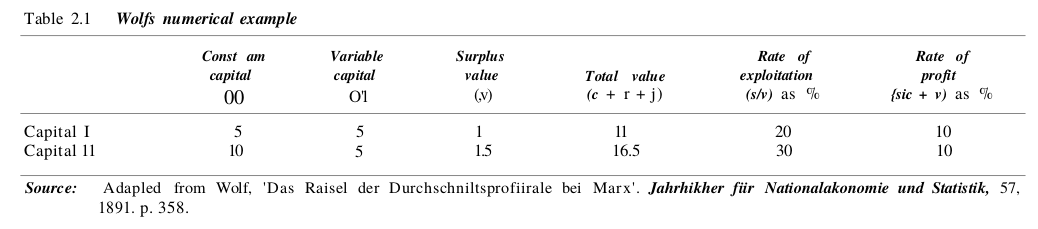
\includegraphics[scale=0.4]{wolfdata.png}
\caption{沃尔弗的数字例子}
\label{fig:wolfdata}
\end{figure}

沃尔弗认为“价值规律并没有被破坏”,在马克思那里不存在自相矛盾的地方。“恰恰相反,
它(解决方法)提供了一个新的证据,证明马克思对于资本主义经济的批判体系,是深刻且
富有远见的”沃尔弗的结论声称整个问题是个伪命题,这一混乱部分地是由恩格斯造成的,
恩格斯试图使先前解决这一问题的尝试都无效,并(沃尔弗隐晦地暗示)推迟了《资本论》
第三卷的出版。无论如何,和斯蒂贝林一样,沃尔弗是\textbf{回避}而不是解决这个问题。

更有意义的的贡献来自彼·法尔曼,施米特称其为“优秀的小伙子、移居美国的俄国犹太人、
职业化学家”。法尔曼受到李嘉图理论的强烈影响。他区分了商品价格中的两个因素:由物
化在商品中的劳动数量决定的商品价值的“\textbf{构成因素}”,以及代表资本家和地主对
产品份额索取权的“\textbf{分配因素}”。法尔曼主张,由于社会财富是由人们生产的商品
中所包含的人类劳动的总量构成的,因此,\textbf{总的来说,价值必须等于价格}:“两种
商品相交换时,一种商品的价格高于它的价值的大小,必然等于另一种商品的价格低于它的
价值的大小,反之亦然”,价格和价值之间差异的产生是\textbf{分配因素}造成的。

他也反对沃尔弗的结论,因为\textbf{沃尔弗认为价值量会随着劳动生产率的提高而增加,
  这和马克思的观点是矛盾的。}法尔曼非常清楚地说明了每个部门的价格、价值和资本有机
构成之间的关系:

\begin{quotation}
  如果利润是剩余价值的表现形式,怎么能够认为在剩余价值量取决于工人数量的同时,
  利润量似乎是独立于工人的数量的呢?仅仅因为,投资在生产资料上的资本和投资在工资
  上的资本之间的比率(或者像马克思说的那样,不变和可变资本之间的比率 $c:v$)最大的产
  业部门,其商品以高于它们价值的价格出售,这意味着,不变资本和可变资本的比率最小
  的产业部门,其商品以低于它们价值的价格出售,$c:v$ 的大小代表着明确的平均水平时,商
  品才按照它们的实际价值出售。
\end{quotation}

这同价值规律并不矛盾,因为总价格仍然等于总价值。个别商品的价格与价值之间的差异
只是竞争引起的波动造成的。“但是在严密的科学中,人们从来不把可精确计算的波动理解
为对规律的否定”。

法尔曼通过强调\textbf{总价格和总价值相等}(莱克西斯强调\textbf{总利润和总剩余价值
  相等})对莱克西斯的工作做出了补充,但是他对有机构成与价格和价值之间偏离关系的分
析更为严密一些。和莱克西斯不同,法尔曼用一个简单的数字例子讨论转形问题,同时对自
己的解决方法进行了一般化处理,以使之能够包含地租和利润的支付,但是这两点并没有被
很好地加以展开,法尔曼对利润率和所用资本关系的分析,表现的并不比施米特更好。

慕尼黑的教授莱尔博士反对沃尔弗的观点,沃尔弗认为,在马克思那里,生产率不同的劳动
创造出不同的价值。莱尔文章最重要的部分是他对转形问题的代数表述,这些代数表达式预
见到了后来德米特里耶夫和\textbf{(尤其是)博特凯维兹}的数学分析。

对整个经济而言,相应的加总分别为K, V和M,他采用了和马克思相同的立场,
用$M/(K+V)=r$ 表示平均利润率。“每单位商品的交换价值”用$t_1, t_2, \cdot $ 表
示(这事实上等同于博特凯维兹的价格—价值比率,即生产价格和劳动价值的比率)。

\begin{figure}
\centering
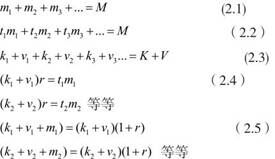
\includegraphics[scale=1]{laier.jpg}
\caption{莱尔的等式}
\label{fig:laier}
\end{figure}

等式(2.1)和(2.2)一起表示总利润等于总剩余价值。等式(2.3)纯粹是定义性的,而等
式(2.4)和(2.5)是试图把每个部门的剩余价值同利润,价值同生产价格联系起来的不成
功的尝试。\textbf{因为它们假定在单个部门内部,价值量和价格量是相等的,这样的假设
  是完全错误的。}……事实上,莱尔唯一直接的推论是\[t_1=t_2=t_3= \ldots = t_n=1 \]

\textbf{这个等式,只有在所有产业的资本有机构成相同的情况下才成立}。莱尔再次没有能够说明马
克思的原理,即$t_i$ 可能大于也可能小于单位值,因为不同产业的资本有机构成可能超过或
低于社会平均水平的资本有机构成,但是莱尔的确提供了一个隐含地表达了这种观点的算术
例子。

作为一个自称为“庸俗经济学家”的学者,莱尔对马克思的价值理论并不十分认同,不大可
能有太多的热情为马克思主要的分析性问题作出解答(虽然他在一定程度上是这样做了)。
莱尔的文章充满了对劳动价值论的批评,其中的一些内容有着强烈的现代说法。莱尔反对只
有在不存在技术进步的情况下,历史的物化劳动和实际的必要劳动才相等的观点,因为随着
时间的发展,技术进步降低了生产商品所需的劳动投入。\textbf{可供选择的其它生产方法
  的存在(比如使用肥力存在差异的土地)使得“必要劳动”的定义变得含糊不清;}无论是
直接地还是间接地,就维护人类生存的体系而言,几乎所有的人类活动都是必须的,因此从
资本主义社会整体的视角看,所有劳动都是必要的,不存在什么剩余劳动。

这些观点中,没有任何一个和转形问题直接相关,但它们的含义\textbf{远远超过了当代新
  古典主义对马克思的批判},并且他很早就预见到那些在斯拉法《\textbf{用商品生产商
  品}》出版后才出现的思考。很明显,莱尔是一个充满活力和原创性的马克思理论的批判者,
恩格斯和后来的马克思主义者对他的忽视实在令人难以理解。

\section{恩格斯的裁决}

恩格斯在为《资本论》第三卷撰写的序言中,用较大的篇幅对参赛者进行了评价。虽然他
没有颁发奖品,但是对莱克西斯、施米特和法尔曼进行了赞扬。莱克西斯是“一个伪装成庸
俗经济学家的马克思主义者”。“我们看到”,恩格斯对莱克西斯的文章评论道,“问题在
这里远没有得到解决,尽管已经含糊地、肤浅地,然而大体上正确地被提出来了”。恩格斯
认为,这已经是可能从莱克西斯那样背景的人那里得到的最多的东西了。法尔曼“实际上已
经接触到了问题的关键”,恩格斯说,“但是,他这篇如此重要的论文所受到的不应有的冷
遇却证明,……仍然需要有许多中间环节,才能完全地、明确地解决这个问题”。至于施米
特,他是第一个真正试图解决(与叙述相对)这一问题的人,但是他没有成功;认为剩余产
品价格的决定区别于不变资本和可变资本价格的决定,事实上等于抛弃了价值理论。施米特
发表在《新时代》上的论文同样是错误的。在恩格斯看来,施米特的真正成就是他分析利润
率下降趋势、商业利润、利息和地租的内容。

在恩格斯看来,沃尔弗只是愚弄了他自己。马克思在《资本论》第一卷有上百处,说的正是
和沃尔弗“解决方法”的基础相反的话。“\textbf{说什么马克思认为在可变资本减少时相
  对剩余价值的增加和不变资本的增加成正比,而这个断言令人如此吃惊,足以使一切议会
  辞令相形见绌}”。

\chapter{价值理论的第一次争论:1895-1914年}
\label{chap:1stzhenglun}

\section{《资本论》第三卷}

在《资本论》第一卷中,马克思简要提及了自由竞争的存在给其价值理论带来的难题。在
《资本论》第三卷第二篇,他对这个难题作了详细阐释,并提出了自己的解决方法。劳动力
市场的竞争造成\textbf{所有产业利润率的平均化},因为在均衡状态下,无论是工作日的长
度还是实际工资的大小都趋于一致,因此,资本家能够从每个雇佣工人那里榨取的剩余价值
量也将趋于相等。如果不同部门的资本有机构成不同——没有什么经济机制确保它必然相
同——它们就将有\textbf{不同的利润率}。产业 $i$ 的利润率被定义为剩余价值和使用的总
资本(不变资本加可变资本)之间的比率:$r_i=\frac{m_i}{c_i+v_i}$ ,把右边个分数的
分子和分母分别除以 $v_i$,得到 $r_i=\frac{m_i/v_i}{(c_i/v_i +
  v_i/v_i)}=\frac{e}{k_i+1}$ ,这里 $e(=m_i/v_i = m_j/v_j)$ 是\textbf{一般剥削
  率}, $k_i=\frac{c_i}{v_i}$是资本有机构成。\textbf{从而,资本有机构成低的产业,
  会有较高的利润率。但是,这与存在竞争的商品市场上的情况不一致,在竞争性商品市场
  中,资本可以从一个产业向另一个产业自由流动,所有生产部门的利润率将趋于平均化。
  因此,在价值规律和自由市场的运行之间存在明显的矛
  盾。}\pagescite[][159-172]{capital3}


在《资本论》第三卷中,马克思表明,要解决这种矛盾,需要对\textbf{劳动价值与长期均
  衡价格之间的有系统的偏离}作出清晰的认识。马克思把长期均衡价格称作\textbf{生产价
  格},他认为生产价格必须处于这样一种水平,即它必须能够包含资本家的成本和用当前的
平均利润率计算的资本家所用资本获得的利润。对个别资本家来说,由于剩余价值完全取决
于劳动中活劳动的数量,利润取决于使用的总资本(死劳动加活劳动),因此剩余价值和利
润也将发生背离。

\begin{quotation}
  就利润来说,不同的资本家在这里彼此只是作为一个股份公司的股东发生关系,在这
  个公司中,按每100资本均衡地分配一份利润。因此,对不同的资本家来说,他们的各份利
  润之所以有差别,只是因为每个人投在总企业中的资本量不等,因为每个人在总企业中的
  入股比例不等,因为每个人持有的股票数不等。\pagescite[][178]{capital3} 
\end{quotation}
 因此,\textbf{价值向价格的转化同时也是剩余价值向利润的转化}。

 资本论中 \pagescite[][174-176]{capital3}的数字例子,清楚地说明了转形问题包含的
 内容。五个部门分别投资100单位资本,每个部门有不同的资本有机构成和相同的剥削率
 ($e=100\%$)。无论是生产出的剩余价值总量还是利润率,和资本有机构成之间都是一种反
 向关系。

 然而,总的来看,\textbf{价格和价值是相等的}(等于442),同样\textbf{总利润也等于
   总剩余价值}(等于110)。这两个“不变条件”的重要性在于,它们使得平均利润率可以
 被定义为两个价值量之间的比率(总剩余价值除以使用的总资本)。马克思推论,一般利润
 率必须“从商品的价值引申出来,没有这种引申,一般利润率(从而商品的生产价格)就是
 一个没有意义、没有内容的概念”。\pagescite[][176]{capital3} 转形过程存在一
 个\textbf{历史的维度}。在\textbf{前资本主义社会}的商品生产中,生产者拥有自己的生
 产资料并相互交换他们的商品,劳动价值成为占统治地位的交换条件。从而
\begin{quotation}
  商品按照它们的\textbf{价值或接近于它们的价值}进行的交换,比那种按照它们
  的\textbf{生产价格}进行的交换,所要求的发展阶段要低得多。\textbf{按照它们的生产价格进行
  的交换,则需要资本主义的发展达到一定的高度。}\pagescite[][197]{capital3}

  因此,撇开价格和价格变动受价值规律支配不说,把商品价值看做不仅在理论上,而且在历
  史上先于生产价格,是完全恰当的。这适用于生产资料归劳动者所有的那种状
  态。\pagescite[][198]{capital3}
\end{quotation}

马克思设想,\textbf{利润率通过资本家之间的竞争而均等化},竞争首先在部门内部展开,
接着出现在部门之间,一般利润率只有到资本主义较晚的历史阶段才出现。

马克思对这个观点没有作进一步的论述,我们随后将会明白,他不这样做是明智的。除此之外,马克思留下了\textbf{另一个没有解决的难题}:
\begin{quotation}
  我们原先假定,一个商品的成本价格,等于该商品生产中所消费的各种商品的\textbf{价
    值}。但一个商品的\textbf{生产价格},对它的买者来说,就是\textbf{成本价格},因
  而可以作为成本价格加入另一个商品的价格形成。\textbf{因为生产价格可以偏离商品的
    价值},所以,一个商品的包含\textbf{另一个商品的这个生产价格内的成本价格},
  也可以高于或低于它的总价值中由加到它里面的生产资料的价值构成的部分。必须记住成
  本价格这个修正了的意义,因此,必须记住,如果在一个特殊生产部门把商品的成本价格
  看作和该商品生产中所消费的生产资料的价值相等,那就总可能有\textbf{误差}。对我们
  现在的研究来说,这一点没有进一步考察的必要。\pagescite[][184-185]{capital3}
\end{quotation}

比如,在表3.1中,五种商品中每一种商品的成本价格,都是按照用来生产这种商品的商品
(不变和可变资本)的\textbf{价值总和}来计算的。但是这些商品是按不同于它们的劳动价
值(特殊情况除外)的生产价格被出售的。然而,\textbf{马克思的“成本价格”完全不是
  价格},接下来的生产价格的计算也就不正确了。正如上述引文指出的那样,马克思发现了
这个困难,但却\textbf{没有提供任何解决它的方法。}

\section{对《资本论》第三卷的早期反应}
马克思对转形问题的分析存在两个重大的难题。假如价值规律在任何时候都可以直接应用,
而在某些情况下却不能发挥作用,这对价值规律的科学地位来说意味着什么?对于马克思在
自己的解决方法中已经意识到、但未能加以纠正的技术性缺陷,能够做些什么呢?恩格斯似
乎没有意识到第二个问题的重要性(参见以上第二章)。他被第一个问题深深地困扰着。他
在生命的最后几个月里,仍然就价值向价格转形的历史问题,同维尔纳·桑巴特和康拉德·施
米特保持着通信,并写下了一篇回复马克思批判者的长文(后来以《资本论》第三卷第二版
的增补发表)。事实上,这个增补成为恩格斯最后一篇重要的、专门研究价值理论的著
述,\textbf{这个增补也成为恩格斯对马克思主义理论最有原创性、也最具争议的贡献之
  一。}恩格斯对价值理论的关注表明,价值理论在所有流派的经济学中都处于十分重要的位
置,对马克思主义政治经济学来讲尤其如此,价值理论在马克思主义经济学对抗新古典学派
时发挥了核心作用。

维尔纳·桑巴特在对《资本论》第三卷的评论中,清楚地说明了价值向价格转形的历史问
题。桑巴特写道,马克思事实上是否打算像坚持价值理论在分析方面具有重要的意义那样,
坚持\textbf{价值理论的形成存在一个具体的历史过程},在《资本论》第三卷中并没有清晰
地展现出来。如果马克思的确有这种打算,那么\textbf{价值理论就包含了逻辑和经验两方
  面的错误}。桑巴特认为,\textbf{价值是一个纯粹的理论概念},它不必也不可能对应着
任何可观察的历史时期,任何试图以这种方式应用价值理论的尝试,都会发现它\textbf{和
  历史事实之间的矛盾}。早期的产业资本家是那些受到更高利润率吸引,并把他们商业资本
的一部分投资于制造业的商人。\textbf{如果在资本主义发展的早期阶段,商品是按照它们
  的劳动价值出售的,那么资本有机构成最低的产业将获得最高的利润率。但是,桑巴特指
  出,事实恰好相反,}资本主义生产关系首先出现在与活劳动使用相比,使用死劳动的比例
最高的产业(比如采矿业)。他认为,\textbf{当代资本主义经济中利润率和资本有机构成
  之间是一种反向变动关系的观点,同样是错误的。}事实上与此相反,高利润率存在于诸如
化工业、酿造业和采矿业等资本有机构成相对较高的产业。\textbf{资本主义产业利润率是
  由竞争的程度},而不是由不变资本和可变资本的比率决定的。因此,任何试图从价值向价
格转形的角度出发,构筑一个有关价格形成的历史理论,都将是完全错误的,转形问题是智
力活动的结晶,而不是现实生活中发生的事情。桑巴特指出,除非恩格斯使他相信相反的东
西,否则他将认为马克思持有和自己类似的观点。\textbf{桑巴特意思是,如果马克思能够
  活着自己准备出版《资本论》第三卷,就有可能消除这些不确定性。}

\textbf{勒克西斯}对马克思作了较多的批评,认为马克思对一般利润率形成的历史描述完全
站不住脚。\textbf{利润率的相等(除了偶然的例外)是资本主义生产的本质}。从来不存一
种社会条件,这种生产条件使得资本主义生产方式同由资本有机构成不同造成的利润率不等
同时并存。\textbf{利润率的相等等同于资本主义的生产方式}并同它们不可分割地联系在一
起。这很像在胚胎中,血液循环的发展等同于胚胎的形状与形式的发展。

康拉德·施米特肯定是了解桑巴特的批评的。……他告诉恩格斯,“价值规律(如果人们把它
当作调节交换的规律而不只是价值的定义)在我看来似乎只是一种虚构,尽管它本身自然不
会是错误的。恰恰相反,\textbf{它是一种必要的虚构},也就是说,它是我们为了得到除此
就无法获得结论而必须作出的一种假设”。就像恩格斯自己在《反杜林论》中表明的那样,
类似的必要的虚构在数学中经常出现。如果没有总价值等于总价格的虚构,将无法得出一般
利润率是由总剩余价值和总预付资本之间的比率决定的这一基本规律。

恩格斯回复施米特:
\begin{quotation}
  您在利润率问题上为什么走上了岔路,我认为,您的来信已经使我得到了一些解释。我在
  这里发现了同一种陷入枝节问题的偏向,我把它归咎于 1848年以来在德国大学中流行
  的\textbf{哲学研究的折中主义方法},这种方法丢掉了事物的总的概貌,过于经常地陷入
  一种几乎是无休止、无结果的\textbf{对枝节问题的思辨}中。

  您对价值规律的责难,从现实的观点来看,涉及\textbf{一切}概念。思维和存在的同一
  性(用黑格尔的话来说)完全符合于您举的圆和多边形的例子。换句话说,这两者,即一个事
  物的概念和它的现实,就像\textbf{两条渐近线}一样,一齐向前延伸,彼此不断接近,但是永
  远不会相交。两者的这种差别正好是这样一种差别,由于这种差别,\textbf{概念并不无条
    件地直接就是现实,而现实也不直接就是它自己的概念。}由于概念有概念的基本特性,就
  是说,它不是直接地、明显地符合于使它得以抽象出来的现实,因此,毕竟不能把它和虚构相
  提并论,除非您因为现实同一切思维成果的符合仅仅是非常间接的,而且也只是渐近线似地
  接近,就说这些思维成果都是虚构。

  一般利润率的情况不就是这样吗?它在任何时候都只是近似地存在着。它们全都没有任何其
  他的现实性,而只是一种近似值,一种趋势,一种平均数,但\textbf{不是直接的现实}。其所
  以如此,部分地是由于它们所起的作用被其他规律同时起的作用打乱了,而部分地也是由于
  它们作为概念的特性。(马恩文集,第10卷,P692-694)

  无论桑巴特还是施米特——至于那位大名鼎鼎的洛里亚,我在这里顺便提到他,只是把他当
  做逗人笑的庸俗经济学的陪衬——都没有充分注意到:这里所涉及的,不仅是纯粹的逻辑过
  程,而且是历史过程和对这个过程加以说明的思想反映,是对这个过程的内部联系的逻辑
  研究。\pagescite[][1013]{capital3} 
\end{quotation}
1895年春,恩格斯完成了名为“价值规律和利润率”的《资本论》第三卷的增补,在对洛
里亚进行回击后,恩格斯总结了桑巴特和施米特对价值概念逻辑地位的分析。无论是桑巴特
还是施米特,“都没有充分注意到:这里所涉及的,不仅是\textbf{纯粹的逻辑过程},而且
是\textbf{历史过程和对这个过程加以说明的思想反映},是对这个过程的\textbf{内部联系
  的逻辑研究}”。不可否认,马克思自己对这个问题的分析只是提供了一个粗略的大纲,毫
无疑问(恩格斯暗示),一旦有机会马克思将对此进行深入的扩充。恩格斯在“增补”的其
余部分中,对填补这个空白进行了大胆的、但最终被证明是难以令人信服的尝试。

…… 商人之间的竞争使\textbf{不同产业的利润率}平均化。后来,随着工厂生产的出
现,\textbf{不同部门的利润率}也被平均化了。这是通过“把一向阻碍资本从一个部门转移
到另一个部门的绝大部分\textbf{障碍清除掉}。这样,对整个交换来说,价值转化为生产价
格的过程就大致完成了”的时候实现的。进一步推动这个过程的事实是,“占有超额剩余价
值的各生产部门,也就是说,可变资本较多而不变资本较少,因而资本构成较低的各生产部
门,按照它们的性质来说,从属于资本主义的经营恰恰是最晚的,而且是最不充分
的;\textbf{首先是农业}”。

这是一个企图从劳动价值论的视角改写几千年经济史的雄心勃勃的尝试,这种尝试的失败并
不奇怪。现代批评者认为,\textbf{在前资本主义社会,商品生产从来就没有充分发展到按
  照商品的劳动价值比率相交换的程度}。重要的领域完全处于商品生产之外;很少有哪个交
易商专门把整个经济活动的时间用于商品的生产;劳动力的流动遇到的强大的体制和文化障
碍,阻止了单位资本收入的均等化;封建主义的剥削关系和商人资本从来就没有完全消失。
因此,除了可能在北美和澳大利亚的殖民地存在过一段短暂的时期外,\textbf{简单商品生
  产几乎从来就没有存在过。}

\section{庞巴维克和希法亭}
庞巴维克在1896年出版的著作中,对劳动价值论进行的新古典主义的攻击产生了较大的影响。
在国际上,无论是与门格尔还是与维塞尔相比,庞巴维克都更为知名,事实上,到世纪之交,
除了阿尔弗雷德·马歇尔,庞巴维克比任何他同时代的人都更加知名。庞巴维克是\textbf{主
  观价值论}的重要倡导者,但他充满原创性的独特的\textbf{利息理论}更广为人知,庞巴
维克用这一理论来取代马克思对资本主义利润的解释。庞巴维克认为,\textbf{资本的使用
  扩展了生产的时间结构},使得使用更加“\textbf{迂回}”的生产技术成为可能。由
此\textbf{导致的投入的使用和最终产出的出现之间的时间间隔的增加},既允许(通过提高
劳动生产率)也要求\textbf{利息的支付}(资本家对当前消费的偏好超过对未来消费的偏好,
在不存在回报的情况下,这会阻止储蓄的发生)。

在任何意义上,庞巴维克都不是一位天生的资本主义辩护者,但他的确在奥匈帝国的学术和
官方体制中,享有受人尊敬的地位。\textbf{他有关“迂回”生产的观点影响了杜冈-巴拉诺
  夫斯基和布哈林}(参见以下第十章和第十五章)。毫无疑问,他对马克思主义的兴趣,因
为与奥地利社会民主党日渐增加的影响作斗争的需要而得到进一步加强。早在1884年,他就
对《资本论》第一卷进行了猛烈的攻击,这是所有对马克思的\textbf{价值分析}进行的正统
批判中的第一次,也仍然是\textbf{最有说服力的一次}。他认为,无论是在演绎方法上,还
是在经验证据方面,劳动价值论都是难以成立的。正如马克思主张的那样,两种商品能够相
互交换,它们之中必然包含了一些共同属性。但是在考察商品交换条件时,马克思在抽象掉
商品的使用价值后,\textbf{错误地否定了效用也可以成为商品的共同属性}。这是一个“最
粗糙的逻辑错误”,\textbf{它混淆了从一般属性进行抽象和从这种一般属性的特殊形态进
  行抽象。}即使忽略掉使用价值,商品仍然存在许多其它与交换相联系的共同属性,比如商
品的\textbf{稀缺性}、它们都是供求的对象,都被私人占有,也都是自然的产物等等。

在庞巴维克看来,劳动价值论也无法被经验所证明。它不适用于那些不能自由地再生产出来
的商品(包括土地),也不适用于那些由熟练劳动生产出来的商品,《资本论》对熟练劳动
的分析是极其不充分的。\textbf{工资非常低的工人生产的商品有着非常低的价值}。此
外,\textbf{劳动价值论只适用于作为(如果成立的话)价格长期波动的中心。在短期内,
  供求占据支配地位。}最后,在1884年的著作中,庞巴维克暗示了后来广为人知
的\textbf{转形问题}——包含同样数量“社会平均劳动”的两种商品,会因为用来生产它们的
资本的耐久性的不同而有不同的价格。因此,价值理论“对于很大一部分商品是完全不,对
于其余的商品总是不、甚至是绝对不”适用的。劳动价值法则与一般价格法则的关系,就
同“\textbf{刮西风便下雨}”的法则与“\textbf{下雨}”的一般理论的关系一样。庞巴维
克清楚地表明马克思的分析同洛贝尔图斯的分析一样,存在的\textbf{主要缺陷就是“与事
  实相矛盾”,这种矛盾源自把“平均利润率规律”和可变资本是剩余价值的唯一源泉连接
  在一起。}马克思同洛贝尔图斯的不同之处在于,他承认了这个矛盾。“但是他犯下的仍然
是这个错误,而不是别的什么错误”。

十二年后,庞巴维克看到了《资本论》第三卷的解决方法……“我感到困惑,在这里,我看
到的不是对矛盾的解释和调和,而是赤裸裸地暴露了矛盾本身,马克思《资本论》第三卷同
第一卷是相矛盾的”。马克思提出的为劳动价值论进行辩护的四个论点,没有一个是令人满
意的。第一个论点(总价格等于总价值)与主题毫不相干,因为\textbf{价值理论涉及的是
  相对价格而不是绝对价格的决定问题}。第二个论点认为\textbf{价值规律支配价格}(而
不是价格水平)的运动,也是错误的。马克思证明的只是\textbf{劳动的量的变化是价格运
  动的一个原由,而不是物化劳动是价格运动的唯一决定因素。}庞巴维克\textbf{没有注意
  到}另一点,即由于\textbf{一般利润率}被认为是劳动价值的比率,\textbf{因此生产价
  格本身是由价值决定的。}一旦在物化劳动量保持\textbf{不变}的情况下,\textbf{工资
  的变化改变了均衡价格,马克思的第四个论点就崩溃了。}庞巴维克把第四点当成天大的难
事:对马克思来说,实际工资等于工人消费的工资商品中\textbf{由物化劳动量决定的劳动
  力的价值}。为了证明他对这一点的批判,庞巴维克需要对马克思工资理论作出正面攻击,
但是他并没有作这样的尝试。

庞巴维克对马克思第三个论点——和\textbf{价值转化为生产价格的历史过程}有关——的驳斥更
有说服力。他认为,马克思在这一点上有点想当然,马克思说明了在应用劳动价值论时交换
是如何进行的,但却没有解释为什么会如此。事实上,庞巴维克坚持认为,没有什么理由能
够说明它应当如此。从本质上看,“对生产者来说,\textbf{什么时候获得他们活动的回报},
是完全无关紧要的”说法,是令人难以置信的。恰恰相反,\textbf{工作的开始和最终产品
  的完成之间经历的时间的长短,是价格决定的一个重要因素,即使是在前资本主义社会也
  是如此。}马克思的观点被历史经验所否定,历史经验表明农民和工匠的收入,实际上受到
他们使用的资本数量的影响。庞巴维克引用桑巴特观点,说明资本主义生产首先出现在有较
高(而不是较低)资本有机构成、相对有着较低(而不是较高)利润率的产业部门。没有任
何证据表明,资本正在从这些产业流出,以寻求更高的利润。这些部门的增长速度实际上要
高于平均水平。

\textbf{桑巴特}通过把价值描述为一个\textbf{逻辑范畴而不是经验范畴}为劳动价值论辩
护。庞巴维克认为这不会令马克思感到满意,\textbf{因为对马克思来说,价值的确是“一
  种真实世界的存在,而不只是思想的构建”。}然而,结论必然就是,劳动价值论从来就没
有被应用过,即使是在原始社会也是如此。这就意味着,马克思主义整个体系,与在它之前
的黑格尔体系一样,是“纸牌堆成的房子”。

1904年,庞巴维克的观点公开出版8年之后,鲁道夫·希法亭对庞巴维克的批判作了唯一一次
系统的、马克思主义的答复。希法亭的反批判由两部分构成,一部分是\textbf{方法论}的,
一部分是\textbf{历史}的。但是,在这两部分中,\textbf{没有任何一部分涉及庞巴维克提
  出来用以反对劳动价值论的具体详细的批评}。这如同后来发生在许多马克思主义政治经济
学领域的争论一样,参与争论的\textbf{双方都未能深入地了解对方的论点,而且缺乏真正
  的对话。}在更为一般性的哲学层面上,希法亭指责庞巴维克总是把\textbf{自然现象和社
  会现象混为一谈}。
\begin{quotation}
  每一种从使用价值出发的价值理论,也就是说从事物的\textbf{自然属性}出发的价值
  理论……是从\textbf{物与人的个别关系}而不是从\textbf{人们之间相互的社会关系}出
  发……这种视角是\textbf{非历史的和非社会的}。它的范畴是自然的和永恒的。
\end{quotation}

劳动价值论不只是,甚至\textbf{不主要是对价格决定的分析}。“正是因为劳动是把分裂为
各个原子的社会联结起来的\textbf{社会纽带},\textbf{而不是因为劳动是技术上最有意义
  的东西},劳动才成为具有现实意义的价值的原则,价值规律才具有现实性”。\textbf{马
  克思的价值论和主观价值论之间的根本区别,远不像庞巴维克认为的那样,只是两种方法
  (可以想象两种方法之间存在互补关系)之间的区别。}这种区别更像是“\textbf{互相竞
  争和互相排斥的观察整个社会生活的视角}”之间的区别。资产阶级经济学的个人主义带来
的完全是\textbf{政治经济学的自杀}。10年后,布哈林雄辩地重新表述了上述对新古典理论
的方法论的批判,并试图表明新古典主义的视角反映了新的“有闲阶级”的观点,这一新阶
级是随着金融资本的兴起而产生的。

在希法亭看来,世界观上的差异和价值转化为生产价格的历史过程紧密相关。在马克思的著
作中,“\textbf{概念的发展完全同历史的发展相平行},因为在马克思主义体系中,社会生
产力的发展,一方面表现为历史现实,另一方面也在概念中得到反映。而且这种平行发展同
时也为理论的正确性提供了最严格的经验证明庞巴维克对劳动价值论在简单商品生产中的适
用性的反对,是没有根据的。因为农民和工匠不可能在不同产业之间自由的流动,利润率的
差异与他们无关。在任何情况下,庞巴维克的分析中提到的资本有机构成之间的重大差异,
指的都是\textbf{资本主义而不是前资本主义经济},这表明庞巴维克的观点是完全无效的。
资本主义工商业中最早出现的有机构成较高的部门,吸引了商人向产业生产的转移,是因
为\textbf{“合法的和事实上的垄断”力量},使得他们能够以高于他们劳动价值的价格出售
他们的商品。在希法亭(把注意力转向了桑巴特)看来,事情的发展顺序如下:商业资本家
开始在制造业中使用他们 “过剩的资本”,然而他们仍然主要是商人。他们从产出数量的增
加和生产规律性的提高,从他们有能力占有工匠生产出来的剩余价值的一部分中获益。“即
使是他们能够保证的,投资在产业中的资本的利润率低于他们可以获得的商业资本的利润率,
然而自此以后他们的总利润仍然是增大了”。最后,资本家进一步从\textbf{更加先进的生
  产方法}中获益,尤其是当特殊的法律赋予他们独占新技术的权利时。“\textbf{直到垄断终结的那
一天……最初极不相同的利润率才有可能平均化}”。竞争首先使个别生产领域的利润率平均
化,随后,资本从一个生产领域向另一个生产领域的自由流动,为整个经济确立了统一的利
润率。

庞巴维克对希法亭的答复完全无动于衷。奇怪的是,希法亭和庞巴维克\textbf{都没有讨论
  马克思转形问题解决方法中存在的技术性难题},合理的推断只能是他们没有注意到这些问
题。希法亭偶尔提及这些问题,表明问题本身并没有激起他足够的信心,使他觉得自己有能
力去解决它们。希法亭\textbf{强调总价值和总价格相等}的重要性,这种相等表明,“所有
的利润都源自生产,而不是来自后来资本家对最终产品产生的任何影响”,希法亭接着给出
了一个大胆的但不合逻辑的断言:“既然总价格等于总价值,那么总利润除了是总剩余价值,
不可能是其他什么东西”。事实上,马克思已经指出了这一点,但是它还没有得到证明。接
下来,希法亭从无根据的断言转向了完全的错误,他宣称,马克思主要关注的是\textbf{工
  资和利润之间的比率},“因此[原文如此]说在关注个别商品时马克思放弃了价值规律,而
只在考察这些商品的总体时才坚持价值规律的有效性,是完全错误的”。希法亭在这里提示
的\textbf{似乎是剥削率与利润和工资之间比率的相等。这是一种妄想}。就像在下一节将要
看到的那样,在一般情况下,马克思的\textbf{两个“不变条件”只有一个能成立}。如希法
亭提示的第三个条件的成立,只能以牺牲上述两个“不变条件”中的一个(或者更有可能同
时牺牲两个)为代价。

争论双方没有任何一方在交流中变得更为完善。庞巴维克对《资本论》第三卷的批评明显不
如他对第一卷的批评。尤其是\textbf{他未能正视马克思劳动价值逻辑优先性的主张},正视
这个主张,就要对马克思一般利润率能够用(且只能用)价值比率加以确定的观点进行反驳。
这反过来对庞巴维克也提出了新要求,他需要对马克思的技术分析,作出比他原本认为的更
多的研究性评价。

\section{米尔普福特和德米特里耶夫}
东普鲁士哥尼斯堡的沃尔夫冈·米尔普福特的社会主义是俾斯麦式的而不是马克思主义
的……米尔普福特的论文和文章,包含两个存在细微差别的\textbf{转形问题的代数表达},
并且非常清晰地指向了20世纪50年代和60年代有关转形问题的数学文献。马克思没有把投入
的\textbf{不变资本和可变资本转化为生产价格},米尔普福特以此为出发点,认为这个问题
可以运用下述方式解决。用 $a_1$ 表示商品1的劳动价值,$x_1a_1$ 表示它的生产价
格,$x_1$ 是价格与价值的比率,这意味着价格是由劳动价值度量的。$p$ 表示一般利润
率,$x_0$ 被定义为 $1 /(1+p)$,马克思意义上商品1的“成本价格”(米尔普福特把它命
名为公司1的“资本价格”)由 $x_0x_1a_1$ 给出。对n个生产不同商品的企业来
说,$a_{11},a_{12},\cdots,a_{1n}$ 是为了生产\textbf{一单位商品}1使用的商
品 $1,2,\cdots,n$的数量;$a_{21}$同理等等。用现代术语来说,它们就是每个产业
的\textbf{里昂惕夫投入系数}。米尔普福特明确地表明,它们是由“各个公司的技术”决定
的。然后,他写下了下列等式:
\begin{gather}
  x_0a_1x_1=a_{11}a_1x_1 + a_{12}a_2x_2 + \cdots  \notag \\
  x_0a_2x_2=a_{21}a_1x_1 + a_{22}a_2x_2 + \cdots \notag \\
  \cdots \cdots \cdots \cdots \notag \\ 
  x_0a_nx_n=a_{n1}a_1x_1 + a_{n2}a_2x_2 + \cdots 
\end{gather}
在上面的式子中,左边给出了每单位不同商品的成本价格,右边是生产它所需的不同商品单
位投入的价格总和。米尔普福特在一定程度上和马克思一样,\textbf{忽视了不变资本和可
  变资本的区别,把工人消费的商品看作是和原材料与机器一样的物质投入。}这是一个在有
关转形问题的现代数学讨论中经常出现的情况,而且很容易被改进为一个更加正统的马克思
的表述式。

米尔普福特得到了n个等式,但是却有$n+1$个未知数(n个价格与价值的比
率 $x1......xn$和用 $x_0$ 表示的利润率),在这一点上他泄气了。他可以做的是,要么
使所有商品的价值总和等于价格总和,要么使总剩余价值等于总利润,得到第$n+1$个等式。
在这两种情况下,他都需要指定第n种商品的产出数量。他未能这样做,而且混淆了马克思的
两个不变条件,把$\sum a=\sum \pi $( $\sum \pi $ 代表\textbf{生产价格总和})写
为:
\begin{gather}
  (a_1 - a_{11}a_1 - \cdots - a_{1n}a_n) + \cdots + (a_n - a_{n1}a_1 - \cdots -
  a_{nn}a_n) = \notag \\
  (a_1x_1 - a_{11}a_1x_1 - \cdots) + \cdots + (a_nx_n - a_{1n}a_nx_n - \cdots)
\end{gather}
这真是\textbf{不伦不类}。左边代表了物化在\textbf{每单位}不同商品中剩余劳动的总量,
右边代表的是与\textbf{每单位}产出相对应的利润。\textbf{这个等式更加近似于第二个不
  变条件(总剩余价值等于总利润)而不是第一个不变条件。}正因为如此,米尔普福特才不
得不用\textbf{产出的数量}去乘以每单位产出的剩余价值和利润。如果
用 $X_1,X_2\cdots, X_n$ 表示商品$1,2 \cdots n$的产出数量,我们可以把:
\begin{gather}
  (a_1 - a_{11}a_1 - \cdots - a_{1n}a_n)X_1 + \cdots + (a_n - a_{n1}a_1 - \cdots -
  a_{nn}a_n)X_n = \notag \\
  (a_1x_1 - a_{11}a_1x_1 - \cdots)X_1 + \cdots + (a_nx_n - a_{1n}a_nx_n - \cdots)X_n
  \end{gather}
当作(真正的)总剩余价值等于总利润的条件。

即使是这样,米尔普福特的代数方法也是失败的,但是他的贡献不仅独具匠心,而且富有成
效,这一点是不可否认的。米尔普福特认为自己是在推动\textbf{古典价值理论和奥地利学
  派边际效用分析的综合},前者解释了\textbf{“自然”(即长期均衡)价格},后者
用\textbf{心理规律说明了稀缺性对短期价格决定的影响}。虽然存在一定的局限性,但奥地
利学派的理论仍然是现有的最佳理论。“从另一方面看,奥地利学派的错误在于试图把他们
的解释方法,应用于自由竞争条件下可自由再生产的商品的自然价格。我的观点是,在古典
学派和奥地利学派之间不存在不可调和的矛盾,这两个体系可以以一种我已经解释了的方式
统一在一起”。

V·K·德米特里耶夫(1868-1913)是当时最重要的俄罗斯数理经济学家。追随着同胞彼得·司徒
卢威和杜冈-巴拉诺夫斯基(参见以下第九章和第十章)的足迹,德米特里耶夫希望能够综合
古典与新古典主义的价值理论。虽然从来没有提到马克思,而且他著作中的大部分内容应归
功于\textbf{瓦尔拉斯}而不是李嘉图,但德米特里耶夫提供了一个\textbf{分析框架},这
个框架\textbf{对后来的劳动价值论和转形问题研究具有巨大的价值。}……论文认为劳动价
值的计算可直接从\textbf{物质投入和产出的技术数据}(马克思经常用其它的价
值——c,v,m——表达价值,从来没有明确地考虑过这个问题)得出。对于商品$A$,$N_A$表示它的
价值(即生产它所需的直接或间接劳动投入的总和);$1/m_i$是生产商品A耗费的第i种商品
的数量,或者,如果第i种商品是机器的话,它表示\textbf{年折旧系数};$n_A$是生产A的
直接劳动投入,德米特里耶夫得到:
\begin{gather}
  N_A = n_A + 1/m_1 N_1 + \cdots + 1/m_MN_M
\end{gather}
\textbf{在这里,劳动价值由直接劳动($n_A$)和间接劳动($1/m_1 N_1+\cdots$)的总和
  决定。}

德米特里耶夫也思考了\textbf{生产价格的决定问题}。然而,他的方法是\textbf{李嘉
  图}式的而不是马克思式的。他\textbf{使用“过去劳动”模型取代了不变和可变资本之间
  的区分}。在这种模型里,不再把商品看作是由直接劳动和生产资料的结合生产出来的,生
产技术被“简化”为由它们作出贡献的时期加以区分的一系列劳动投入。棉纱被认为是纺纱
工的劳动(当年耗费的)、棉花种植者的劳动(去年耗费的)和必要的机器制造者的劳动。
棉纱由此可追溯到两年或更长时间的劳动。忽略掉机器,假定棉花是由不借助外力的劳动者
种植,那我们可以得到原棉和棉纱的“\textbf{过去劳动}”价格方程:
\begin{align}
  P_A &= WL_A(1 + r) \\
  P_B &= WL_B(1 + r) + W\frac{1}{m_A}(1+r)^2
\end{align}
$P_A, P_B$是棉花和棉纱的价格,$L_A, L_B$是种棉花和纺纱活动中每单位产出使用的劳动
的数量;$1/m_A$(再一次)是生产一单位棉纱要求的棉花投入的数量;$r$是年利润率。
则$L_A,L_B$和$(1/m_A)L_A$表示“过去劳动”,每个都被(1+r)的乘方加权,乘方的大小由
劳动被“锁定”在生产中的\textbf{周期的长短}决定。长期均衡价格,定义为资本家过去的
所有工资开支,加上包含所有相关时期以当前的平均利润率为折算系数计算出的复利形式
的利润的总和。简单地说,假定工人只消费谷物,给定时期资本家的支出为$n_AaP_A$ ,
$a$ 是每个时期工人消费的谷物的数量,$P_A$ 是谷物的价格。,$n_A$和前面相同,代表所
需的(这次是在时期A)直接劳动投入。对商品A(谷物)来说,自然价格(生产价格)被定
义为:
\begin{gather}
  P_A = n_AaP_A(1+r)^{t_{A1}} + \cdots + n_MaP_A(1+r)^{t_{AM}}
\end{gather}

r为平均利润率,在得到最终产品之前,劳动投入$n_A \cdots n_M$存在的生产周期
为$t_{A1} \cdots t_{AM}$ 。给定真实工资a,一旦定义了价格计量单位,便可由方程所代
表的方程组解出用技术系数$n_A \cdots n_M$ 与$t_{A1} \cdots t_{AM}$表示的生产价
格$P_A \cdots P_M$和 $r$。这甚至超越了米尔普福特,德米特里耶夫在19世纪的最后十年,
已经预见到了20世纪中叶出现的\textbf{数理经济学}。

\section{冯·博特凯维茨的解决方法}
上述这一切,都没有给西方的社会主义者留下什么印象,也没有对俄国的正统马克思主义者
产生什么影响。然而,德米特里耶夫的著作被有着俄罗斯血统的柏林统计学家拉迪斯劳
斯·冯·博特凯维茨注意到了。博特凯维茨是一个对马克思有着强烈兴趣的李嘉图主义
者……“正如马克思那样,德米特里耶夫的模型,把商品生产的技术条件,包括表现为给定
的实际工资的劳动力商品生产的技术条件,作为价格最终的和唯一的决定因
素”。\textbf{博特凯维茨用德米特里耶夫的代数框架,得出了马克思的剥削率和利润率函
  数(用“过去劳动”数量表示)。}他还说明,在作为货币的商品的有机构成、劳动力价值
和相关产业的生产价格之间存在精确的关系。

然而,马克思和德米特里耶夫之间也存在着重要的区别。博特凯维茨注意到,后者拒绝了马
克思在不变资本和可变资本之间所做的区分,并用代数表达式取代了数字例子。这种区别,
比它们表面上看起来要重要的多,因为它意味着一种重大的方法论上的突破:德米特里耶夫
使用\textbf{同时决定}的方式进行论证,而马克思使用\textbf{因果链条}进行推理,博特
凯维茨批评马克思这种推理是一种“\textbf{连续近似}”的谬误。德米特里耶夫证明了马克
思对李嘉图的批判是无效的,\textbf{李嘉图没有混淆价格和价值,也不需要马克思对不变
  资本和可变资本进行的区分,}李嘉图的主张(被马克思否定的),\textbf{利润率不受某
  些产业生产条件变化的影响},这些产业\textbf{既不生产工资商品也不生产用于(直接或
  间接的)工资商品产业的生产资料,这是正确的。}博特凯维茨在结论中,对马克思进行了
严厉的批判。“毕竟价值计算和价格计算之间有着密切的数学联系,马克思在这个问题上的
分析缺陷,反映了他数学能力的缺乏”。\textbf{马克思认为与价格决定相比,价值决定具
  有逻辑上的优先性是错误的}:“不仅价格、工资和利润率之间的相互关系,可以简化为无
需从价值和剩余价值的数量开始的数学表达式,而且如果使用正确的公式表达的
话,\textbf{价值和剩余价值的数量甚至可以不出现在计算中}”。

博特凯维茨似乎对马克思有些着迷,他的第二篇文章更为直接地分析了《资本论》第三卷中
的转形问题。从概念层次看,这篇文章不如第一篇成熟,\textbf{用三部类模型取代了存
  在n种商品的模型}(另外,对三个部类而言,生产不变资本的产业的\textbf{资本有机构
  成是相同的})。第\Rnum{1} 部类生产生产资料,第\Rnum{2} 部类的产出由工资商品构成,
第\Rnum{3} 部类生产资本家消费的奢侈品。博特凯维茨进一步抽象掉固定资本,所有的资本
每年周转一次,并假定\textbf{简单再生产}居于支配地位。这使得:
\begin{gather}
  c_1+v_1+m_1=c_1+c_2+c_3=C \notag \\
  c_2+v_2+m_2=v_1+v_2+v_3=V \notag \\
  c_3+v_3+m_3=m_1+m_2+m_3=M 
\end{gather}

在这里,不变资本的产出完全等于各个产业使用的不变资本;工资商品的产出正好足以养活
三个部类中的雇佣工人,奢侈品的产出正好等于生产的剩余价值的总量。同米尔普福特一样,
博特凯维茨用$p$表示平均利润率。另外,\textbf{$x, y, z$分别表示三个部类中生产价格
  和价值的比率};这和米尔普福特的$x_1 \cdots x_n$相对应。马克思的转形问题解决方法
要求:
\begin{gather}
  (c_1x+v_1y)(1+p)=(c_1+c_2+c_3)x \notag \\
  (c_2x+v_2y)(1+p)=(v_1+v_2+v_3)y \notag \\
  (c_3x+v_3y)(1+p)=(m_1+m_2+m_3)z
\end{gather}
等式(3.9)是米尔普福特的等式(3.1)在三部门模型中的对等物。等式左边代表(用价格
术语)每个部类的成本价格,乘以(1+p)表明生产价格必须包含成本和利润。右边表示用生产
价格而不是用劳动价值标示的每一类商品的产出。资本家必须从出售他们的商品中获得足够
多的收入(等式的右边)去补偿他们的支出和平均利润率为p时可获得的利润(等式左边)。

博特凯维茨有了(3.9)所表示的三个等式,但却有四个未知数:x, y, z和p。他注意到,那
个缺失的等式可以通过引入马克思两个“不变条件”中的任何一个得到(\textbf{但不是同
  时引入两个})。总价值和总价格的相等使得:
\begin{gather}
  Cx + Vy + Mz = C+V+M
\end{gather}

C, V和M是总量指标,使总剩余价值等于总利润等同于指定
\begin{gather}
  z = 1
\end{gather}
等式(3.10)和(3.11)表达了马克思的两个不变条件。如同博特凯维茨在几个数字例子中
表明的那样,\textbf{一般情况下,两个条件不可能同时成立。}比如,\textbf{在一个
  第\Rnum{3} 部类的资本有机构成低于社会平均构成的模型中采用等式(3.11),将使得价
  格总和超过价值总和,反之亦然。马克思假定是错误的。}只有那些生产工资商品的产业
(直接的或间接的)——事实上,即第\Rnum{1} 部类和第\Rnum{2} 部类,但不包括
第\Rnum{3} 部类——决定了利润率。在这一点上李嘉图是正确的,错误的是马克思。但是,博
特凯维茨提醒道,这种结论不能被推广的太远。这并不意味着部类\Rnum{3} 的资本有机构成
可以无限的大,因为如果它的确很大,那么利润率的均等化将不再可能。\textbf{马克思的
  分析存在问题,但他的本意是正确的。}

博特凯维茨的著作没有产生明显的直接影响。1949年,他的著作的英文翻译者保罗·斯威齐认
为,“有证据表明,它只被少数几个专家阅读过”。斯威齐没有对这些专家的身份进行说明,
就我们所知,1942年出版的斯威齐的《资本主义发展论》,对博特凯维茨的第二篇文章进行
了概括,并引发了对转形问题重要的(和持续的)争论,在此之前,对转形问题进行的认真
分析仅有两次。没有任何一个第二国际的著名理论家关注过这个问题。35年的空白期,折射
出这一时期马克思主义政治经济学科研水平的不足。在这一段暂歇期,对价值理论进行的哲
学思考出现了一些重大的进展,但有关这个问题的技术分析没有取得什么明显发展。直到线
性经济学工具在冯·诺依曼和里昂惕夫的著作(20世纪30年代和40年代)中出现后,对价值问
题“数量方面”的讨论才重新开始。

\chapter{伯恩施坦,考茨基和修正主义论战}

\section{德国社会主义的兴起}
19世纪后半叶,德国经济经历了特别高速的发展,帝国(1871年才成为一个政治统一体)由一个相对落后的主要农业区,转变为世界上重要的工业力量之一。……


与英国相比,德国的工业很大程度上受银行资助,银行获得了大量的股份和对制造能力方面
的控制权。德国银行业高度集中,到1914年,\textbf{五个最大的银行集团控制了全部银行
  资本的四分之三的份额。因而银行鼓励对价格操纵的卡特尔的形成,}卡特尔存在于世纪之
交的大多数产业中,促进了产业集中趋势的进一步发展。它们在海外的活动得到扩大,以至
于在19世纪80年代,德国已经成为\textbf{净资本输出国}。30年后,帝国的资产总计
达300亿马克,三倍于全国的年出口收入。在德国进行工业化的最初几十年里,贸易壁垒逐步
降低,直到遇到开始于1873年的严重萧条,这时候,来自北美的谷物和英国的生铁引起的竞
争,迫使大企业和容克都要求政府进行干预。1880年后,德国的市场再次受到\textbf{关税
  保护}。这只是国家普遍并越来越深入地参与经济活动的一个方面,这种参与还包括政府或
市政拥有铁路、矿山、工厂和公共设施的所有权,还包括\textbf{俾斯麦式的社会立法},这
些法律要求为疾病、意外事故和养老提供强制性的保险,对妇女、儿童的工作时间进行控制。
到1914年,德国已成为一个有着\textbf{强大社团主义因素的混合经济}。

帝国的社会结构密切地反映了它的经济基础。除大企业和工厂的无产阶级外,还存在一个
代表强大的准封建利益的地主;一个只能算是半无产阶级的且深受压迫的重要的农业工人阶
级;一个数量巨大、通常比较富裕的农民阶级,这个阶级在德国的南部和西部尤为明显;一
个经常变化的,由各种类型的城市商人、手工业者和小雇主构成的中产阶级下层。从政治和
文化方面看,\textbf{德国处于完全发展的资产阶级社会和旧体制的中间地带},前者的典型
代表是美国,后者的典型例子是罗曼诺夫专制政体。特别是在普鲁士,前资本主义制度以及
与之相适应的价值观念和行为方式仍然占主导地位,即使是在非常先进的资本家圈子里也是
如此。土地财富、军队和宫廷仍然拥有远远超过马克思主义理论家们认为的影响力。

当时德国的中层和上层阶级的观念非常保守,而且具有强烈的\textbf{民族主义倾向},既没
有同时代法国存在的反教权的激进的共和主义,也没有格莱斯顿时期英国兼容并包的自由主
义。上层资产阶级已经同贵族统治阶级结盟。同欧洲其他许多地方一样,贵族统治者的世界
观占据主导地位。雇主几乎普遍地敌视工会,这更多的是由于担心被颠覆,而不是由于对劳
动力自由贸易教条式的坚持。英国模式中存在的集体谈判和工业调解,在德国发展的非常缓
慢。在受人尊敬的德国政坛谱系的最左端,站的是“教授社会主义者”(讲坛社会主义者)。
像古斯塔法·冯·施穆勒和阿道夫·瓦格纳这些人,更多受到的是洛贝尔图斯的而不是马克思的
影响,试图把对不受约束的资本主义竞争的怀疑、对福利立法的支持,对德国政府以及德国
正在迅速发展的军事机器毫无异议的忠诚结合起来。

德国社会主义深深扎根在这片明显贫瘠的土地上。1875年,在哥达统一会议上,成立
了SPD——众所周知的德国社会民主党(the Social Democratic Party of Germany)的缩
写,SPD的成立是以一个马克思对它进行过严厉的批评、存在着一定程度的混乱和折中的纲领
为基础的。德国社会民主党无论在人数上还是在影响力上,都得到极为迅速的发展。三年后,
带有压制性的“反社会主义者非常法”没有影响社会民主党的选举活动,只是使党的宣传活
动变得更加复杂,但没有完全阻止党的宣传活动。SPD同迅速扩大的“自由”(非教派的,独
立于雇主的)工会建立了密切的联系,为了广泛地开展党的宣传工作,组建了一支庞大的由
付薪雇员组成的队伍,这支队伍中包括一些组织者、讲演者和新闻记者。到1914年,SPD的成
员已超过1百万,和它有联系的工会会员超过250万。在1912年的选举中,人口在1万或1万以
上的城镇中,SPD差不多赢得了接近一半的选票。当时,完全有理由相信,德国社会民主党会
取得更大的成功。德国社会民主党吸引了来自奥匈帝国、俄国以及德国国内的激进分子。它
的辩论受到密切的关注,它的纲领被深入研究,它的知识分子受到越来越多的尊重,在欧洲
内外都是如此。

总之,德国社会民主党是国际社会主义运动皇冠上的明珠,\textbf{是当时世界上最大的和
  最重要的马克思主义政党。}无论是在实践方面,还是在意识形态方面,它对第二国际都起
着主导作用。

\section{正统马克思主义和《爱尔福特纲领》}

考茨基负责被视为“正统”马克思主义的社会主义理论文献的制订和传播工作,在这一点
上,考茨基的贡献甚至比恩格斯还要大。这里谈到的“\textbf{正统}”马克思主义,同马克
思本人的思想相比,出现了\textbf{两个微妙但却是根本性的变化}。第一,作为马克思早期
著作的特点,并在马克思晚年某些著作中仍然保留的\textbf{黑格尔主义和人道主义的特征},
在很大程度上\textbf{被更为常见的实证主义方法所取代},资产阶级在对当时资本主义社会
的批判中广泛接受了实证主义方法。\textbf{严格的因果逻辑、趋势预测和决定论,逐渐脱
  离了马克思的辩证的先验论的范畴。}第二,\textbf{进化论的科学的自然主义被引进马克
  思的思想,随之而来的是有关国际和平、社会经济进步和科学认识日渐进步的乐观信念。}特
别需要注意的是,卡尔·考茨基在成为马克思主义者之前是一个达尔文主义者,他的哲学观点
更多受到的是《\textbf{反杜林论}》的而不是马克思早期著作的影响。考茨基把马克思主义
看作是\textbf{历史科学},他自己的马克思主义政治经济学牢固地建立在这一基础之上。

党开始考虑用一个新的原则声明取代难以令人满意的哥达纲领。新宣言中有关实践的部分,
交由德国社会民主党的议会领袖奥古斯特·倍倍尔和伯恩施坦负责,根据恩格斯的指示,考茨
基负责理论部分。最终形成的《爱尔福特纲领》指出:资本主义必然导致生产者的生产资料
被剥夺,小企业被大企业取代,由农民与小资产阶级构成的中间阶层将最终消失;技术进步
的一切利益都被资本家和地主独享,同时工人遭受苦难和无保障不断增长;阶级对立日益尖
锐;经济危机进一步加剧了这种对立,经济危机的根源在于资本主义生产方式的本质,经济
危机一天比一天扩大,越来越具有毁灭性;只有通过无产阶级协调一致的政治行动废除私有
制,才可能使人类的生产力得到充分的发展。

1892年,考茨基在他的著作《阶级斗争》中对纲领进行了系统的辩护,《阶级斗争》对资本
集中和经济危机的原因作了极为详细的说明。考茨基论证道,\textbf{资本集中和经济危机
  这两种现象密切相关。}信用不只是一种资本集中、剥夺非资本主义部分的人口、促进经济
快速发展的手段。它也是一种“使现代生产方式变得日益复杂并对一切干扰日益敏感的机体,
使资本家日益感到不安并使他们的活动基础愈加不稳”的手段。\textbf{危机是生产过剩的
  结果},而这种生产过剩是由资本主义生产的\textbf{无计划性}造成的。经济扩张的越快,
需求预则就变得越困难,市场条件的不确定性就越大,投机也就越疯狂。托拉斯和辛迪加无
法消除危机,无法阻止国际竞争,它们只能造成\textbf{资本家敌对集团之间“你死我活的
  斗争”}。

考茨基把资本主义生产的无政府状态解释成经济危机的原因之一,而日益增长
的\textbf{需求不足}是他分析危机产生的另一个原因。利润率下降趋势以一种\textbf{间接
  的方式}对危机产生冲击。……“\textbf{利润和利息的下降并不是资本家阶级的灭亡,而
  只是它的范围的缩小}”。反过来,这又成为生产过剩危机的一个重要因素,因为资本集中
以及它所推动的剩余价值的再分配,使得剩余价值开始从消费收入比大的小资本家向消费收
入比相对较小的大资本家转移。工人阶级消费的增长因失业率的上升而受到限制。

考茨基认为,结果将是长期的生产过剩和比以往任何时候都更加频繁、更加猛烈的危机。
从长期来看,国内需求的不足,无法由市场出口的扩大相抵消。因为最有利可图的市场已得
到充分的利用,剩下的尚未开辟的是那些“除了热带病和挨一顿棍棒之外,什么也得不
到”的市场。此外,资本主义生产在世界上迄今为止仍不发达的地区开始出现,通过创造自
己的竞争对手,“资本主义大生产为自己挖掘了坟墓”。市场的扩张最终将不再可能,
这“将意味着整个资本主义体系的崩溃”,它也已经“开始在自己的剩余中窒息”。考茨基
的推论是,资本主义将完成它的历史使命,未来的社会主义共和国取代资本主义的时机已经
成熟(这个主题,成为他这部著作下半部分的主要内容)。

《阶级斗争》用简单而形象的语言写就,坚持认为\textbf{迫在眉睫的社会变革即将来临},
成为一本具有重大影响的著作。除了恩格斯偶尔作出的思考(许多最重要的思考是三年后
《资本论》第三卷出版时才作出的),《阶级斗争》是唯一一次把马克思主义政治经济学
和19世纪90年代的实际情况相结合的认真尝试。至少在当时,这本著作的不足之处被掩盖
了……但是《阶级斗争》中的缺陷确实存在,无论是从经验上还是从理论上看,《阶级斗争》
都不能算是一本令人信服的著作。考茨基有关资本集中、无产阶级贫困加剧、利润率下降与
收入和财富不平等加剧的判断,并没有被任何严肃的统计调查数据所证明;而且《阶级斗争》
明显地缺乏马克思使用过的细致的历史研究方法。考茨基对卡特尔、信用、危机和崩溃的说
明,更多的是一种断言而不是严格的分析。\textbf{不确定性在经济波动中的作用,直到今
  天仍然是一个极具争议的复杂问题,在对这个问题的理解上,对考茨基期望过高是不公平
  的。}

\section{伯恩施坦对正统的挑战}
重要的是要记住,德国社会民主党的理论家几乎无一例外都是记者或政治活动家,而不是学
者,即使是他们最抽象的作品,也是面向\textbf{具体的战略和战术问题}的。然而,事实上,
理论和实践之间的联系远没有修正主义争论的参与者认为的那么紧密。德国社会民主党的党
员很少有对理论细节表现出极大兴趣的,党的领导人往往对发生的具体事件做出务实的反应,
而不是始终如一地应用马克思主义分析的基本原则。争论的参与者并没有清楚地认识到这一
点。结果修正主义争论同时具有了政治分裂和理论辩论的双重特征。

在考茨基那里也存在含糊不清的地方,1893年,他把德国社会民主党定义为“\textbf{一个
  革命的,但不制造革命的党}”,并且否认无产阶级发起社会革命的权力要大于资产阶级阻
止革命发生的权力。阶级斗争在加剧:党必须作为独立的工人阶级组织参与其中,但是这一
切将如何结束?

\textbf{在英国,没有可供谈论的革命的社会主义政党。革命党的位置被稳固而又成功的工
  会运动和一个强大而又激进的游说集团占据},游说集团通过议会立法完成重要的社会改革。
伯恩施坦深受英国费边主义和“新自由主义(New Liberalism)”的影响,后者代表了左翼
中产阶级的观点,并和费边主义保持着密切的联系。

当然,伯恩施坦和恩格斯有着十分密切的关系,但是,恩格斯的巨大的权威性,也被伯恩
施坦用来反对德国社会民主党的革命言论、用来捍卫通过和平改革的方式实现社会主义的主
张。事实上,恩格斯去世前一年为马克思《\textbf{法兰西阶级斗争}》所写的导言,已经被
公开地解释为(如伯恩施坦解读的那样)第一篇重要的修正主义文献。

1899年,伯恩施坦出版了一本更加系统的论述修正主义的著作——《社会主义的前提和社会民
主党的任务》,这本书以《进化的社会主义》为名被译成英文。

他相信,可靠的唯物史观可以被用来反对过度的“极端马克思主义”,但是这种反对,只能
建立在康德的而不是黑格尔的哲学基础之上。事实上,他以把自己描绘为康德式的社会民主
的支持者结束了自己的著作。

\textbf{康德否定了实证主义的科学观,}这种观点只把建立实际观察到的事物之间的规律性
联系视为科学的任务,\textbf{强调取消认知主体在知识构建中的优先地位}。虽然马克思主
义者因认为\textbf{康德哲学具有非历史性的特征}而经常批判它,但康德哲学\textbf{并不
  一定必然}和马克思在《巴黎手稿》或者《关于费尔巴哈提纲》中所表达出来的哲学思想相
对立,这两本著作中的哲学思想影响了奥地利马克思主义者和法兰克福学派。然而,新康德
主义很难与恩格斯和考茨基的\textbf{实证主义唯物论}相调和,而且实际上向占主导地位的
正统马克思主义提出了重大的哲学挑战,尤其是对正统马克思主义关于自然科学和社会科学
所作的同化提出了重大挑战。伯恩施坦取得的成就,要比他可能取得的少的多。他不是一个
哲学家,他是一个\textbf{折中的经验主义者},也是一个始终如一的\textbf{新康德主义
  者}。

伯恩施坦的理论特征,在他对马克思主义价值理论的批判上表现得特别明显,比如,他借鉴
了庞巴维克的反对意见(参见以上第三章的概述),在很大程度上赞同边际效用分析,但他
并不主张放弃劳动价值论。伯恩施坦反对马克思对不同工人之间技能、速度和效率差别的分
析,赞同俄国学者\textbf{利奥·冯·布赫}的观点,\textbf{认为个别工人耗费的劳动数量只
  能通过参照他们获得的工资去度量}。除非以这种方式定义,\textbf{否则价值概念就只是
  一个“纯粹的假设,一个没有任何实质内容的思维建构”}。……伯恩施坦并没有被恩格斯
为劳动价值论进行的历史辩护说服(参见以上第三章),\textbf{他同意康拉德·施米特的意
  见,如果劳动价值只是普遍存在于前资本主义经济中,那么把劳动价值概念应用于资本主
  义时,它就只代表“一个纯粹的公式”、“一种抽象”、“一个纯粹的抽象概念" 。}如果
把同样的逻辑用于边际效用理论,那么,能够得出的结论是,新古典主义和马克思主义理论
有着相同的本体论基础,因此,没有任何先验的理由去拒绝一个而支持另一个,两者都有其
用途。

在剥削理论上,伯恩施坦又一次试图调和马克思主义和新古典主义方法。他指出,剩余劳动
是“\textbf{一个经验事实,可以被经验证明,不需要什么演绎证明}”,劳动价值论除了
是“一种分析和说明的方法”之外和剩余价值无关。……此外,伯恩施坦还认为,在衡量剥
削程度时,马克思的剩余价值率是一个具有误导性的指标。商品按它们的生产价格而不是劳
动价值出售,从而使得对个体而言的剩余价值率,变得无关紧要。

伯恩施坦攻击的第三个批判对象是马克思的工资理论。1901年,他指出,工人阶级因地区
和(特别是)职业的不同而开始不断分化。像工会那样,现代技术在工人阶级中造成整合和
分化的趋势,但不能确定地说哪一种将占主导地位。但是,工人的工资差别很大且在不断扩
大。伯恩施坦认为,这些事态的发展使得传统马克思主义越来越不切实际,因为传统马克思
主义把工人阶级视为一支单一、同质的力量,使得失业的产业后备军更像是一种抽象而不是
现实。

伯恩施坦第四个反对意见是针对马克思关于资产阶级的观点,特别是针对生产资料迅速集中
到少数人手中的看法的。……税额和股权分配的数据表明,财产所有权的分散广泛存在并可
能逐渐扩大,而不是正统马克思主义者预测的越来越集中。事实上,为了解释消费品行业产
出的扩大是如何在国内市场找到盈利渠道的,是需要类似情况的。

这些结论把伯恩施坦直接引向他的批判的最后的、也是最重要的部分,在这一部分他抨击
了认为经济危机将不可避免地变得越来越严重的正统观点。

在《社会主义的前提和社会民主党的任务》中,伯恩施坦表明的最流行的社会主义者的危机
理论是以\textbf{消费不足}的方式提出的。但是,这已经被恩格斯在《反杜林论》中和马克
思本人(经过最初的犹豫)\textbf{否定}了,因为这在无产阶级和中产阶级的购买力都在稳
步扩大的经济中,是完全站不住脚的。(Note: 可参阅“消费不足论”还是“生产过剩
论”——评马克思主义经济危机理论早期的一个争论”。 \url{http://www.docin.com/p-1421218945.html})

伯恩施坦认为,马克思在晚年的著作中还提到危机的另外两个原因。一个是由投资支出的积
聚和更新引致的“\textbf{回波效应}”\footnote{回波效应是由1974年诺贝尔经济学奖获得
  者冈纳·缪尔达尔(Gurmar Myrdal,)提出的。所谓的“回波效应”是指经济活动正在扩
  张的地点和地区将会从其他地区吸引净人口流入、资本流入和贸易活动,从而加快自身发
  展,并使其周边地区发展速度降低。 回波效应是指别国由于”溢出效应”所引起的国民收
  入增加,又会通过进口的增加使最初引起“溢出效应”的国家的国民收入再增加。},但是
这一原因原则上是不太可能的,而且也无法被任何证据所支持。另一个认为在再生产过程中
存在\textbf{比例失调},这种比例失调是由\textbf{资本主义生产的无政府状态}导致的,
并且因\textbf{世界市场的增长与财富和信用的大扩张}而得以加强。伯恩施坦认
为,\textbf{相反这些发展为有序的调整提供了更多的机会。}在不引发普遍的危机的情况下,
特定行业的生产过剩越来越有可能被避免或消除。通讯条件的改善,使得信息的传递更加便
捷和安全。卡特尔和托拉斯能够调节生产并保持更加稳定的价格和产量。由于无法预见的外
部事件的存在,危机仍然是可能的,但它们已不再是无情的经济规律的必然结果。那种认为
资本主义由于其内在矛盾行将崩溃的普遍期望是没有根据的。

\section{卢森堡和考茨基的回应}
伯恩施坦的大部分批评只是\textbf{尚待证实的断言},而不是严密推理的结论。这在一定程
度上反映了他作为理论家的不足,在一定程度上也是因为修正主义争论的内在本质造成的。
对于积聚、集中、社会两极分化或无产阶级意识的增长程度,并不存在公认的评判指标;因
而对于这些现象中存在何种程度的趋势来判断支持争论中的这一方还是那一方,并没有统一
的标准。和修正主义相类似的缺陷,在《阶级斗争》中也可以找到,但有理由认
为,\textbf{经济事实}是站在伯恩施坦一边的。伯恩施坦最终受到的抨击是围绕他
的\textbf{理论基础}展开的,伯恩施坦的批评者通过对正式的危机和崩溃模型的详尽阐述,
通过对垄断、金融资本、帝国主义和战争之间的联系展开的不是很严密的分析,对伯恩施坦
进行了批评(参见以下第五章、第六章、第十三章、第十四章和第十六章)。然而,正统马
克思主义者最初的反应是论辩性的而不是学术性的。\textbf{正统马克思主义者最初的反应
  是论辩性的而不是学术性的}。毫无疑问,先行者应当是卡尔·考茨基,但他却被年轻、积
极、雄心勃勃的罗莎·卢森堡抢了先。

卢森堡认为,科学社会主义有三大支柱构成:第一,“资本主义经济中不断增长
的\textbf{无政府状态}”,最终将导致资本主义\textbf{毁灭};第二,\textbf{资本主义
  生产社会化程度的增长,孕育了未来社会主义秩序的萌芽};第三,\textbf{无产阶级的组
  织和阶级觉悟}在不断增长。伯恩施坦否定了第一个论点,但却拒绝回答一个明显的问
题:“究竟我们为什么还能够达到和怎样才能够达到我们的奋斗目标呢?”伯恩施坦把第二
个和第三个论点看成是阻止危机发生和促进和平进步的因素,从而使社会主义革命似乎成了
多余的东西。针对这种观点,卢森堡认为,信用和卡特尔的增长加剧了\textbf{生产和消费
  之间的矛盾},加深了\textbf{危机的严重性}。信用的扩张往往通过具有内在不稳定性的
投机活动引起生产的扩张,然后,当信心开始动摇的时候,它迅速地减少了消费,因
为“\textbf{危机刚刚露出苗头,信用就紧缩了}”。卡特尔远不是消除资本主义矛盾的“适
应手段”,在卢森堡看来,它只是“加剧资本主义固有的无政府状态”的手段。卡特尔要提
高一个生产部门的利润,就只有牺牲别的部门的利益。但它无法阻止整个经济“利润率的致
命下降”。

重要的是,卢森堡(追随考茨基)\textbf{把利润率的下降看作是资本集中的手段,而不是
  危机的主要原因}。以上引述的内容,似乎是她唯一一次对利润率趋势问题非常认真的分析。
在《社会改良还是社会革命?》这一小册子的后面部分,卢森堡认为,\textbf{军国主
  义}是“不可避免”的,它为资本家的“金融和产业资本提供最重要的投资形
式”。\textbf{国内利润率下降导致的资本输出,推动了希法亭—列宁帝国主义理论的出现},
如果卢森堡的上述分析算得上是希法亭—列宁帝国主义理论胚胎中所包含的东西,那么这种类
型的帝国主义理论在卢森堡这里算得上是胎死腹中了。

在早期的争论中,不存在任何有资格被称作危机理论的内容。因为资本主义生产的无政府状
态、生产和消费之间的矛盾这种口号式的东西,只能算是\textbf{危机理论肤浅的表达}。伯
恩施坦在反对卢森堡的信用和卡特尔的功能的观点时,没有遇到什么困难,与此同时,他对
卢森堡提出的关于德国社会主义党的“最终目标”如何实现这个问题的回答,成为修正主义
的著名的格言:
\begin{quotation}
  \textbf{我对人们通常所理解的“社会主义最终目的”的东西极少有热情和兴趣。这个目
    的无论是什么,在我看来都是微不足道的,运动就是一切。我所理解的运动就是社会的
    总运动,即社会进步,也是为促成这一进步而进行的政治上和经济上的宣传和组织工作。}
\end{quotation}

卡尔·考茨基的《反批评》一书作了更具实质性的努力。同卢森堡的批判一样,政治是这
本书的核心。考茨基的政治基石是这样一个信念,即资本家的利益和工人的利益是完全不可
调和的。因此,无产阶级必须继续独立于其它阶级,社会民主党必须完全独立于所有其他党
派。

《反批判》的特色在于它以方法论问题作为开篇。考茨基认为,伯恩施坦批评马克思的方法,
但却未能找到任何替代的方法,而且仍在(不一致地)继续使用它。修正主义对唯物史观的
反对是错误的,因为马克思主义\textbf{强调的是阶级斗争而不是机械的必然性}。紧接着是
简短但难以令人满意的论述价值理论的一章。在这个问题上,考茨基对伯恩施坦作出的唯一
让步,涉及熟练劳动化简为非熟练劳动的问题,关于这一点——他承认——马克思本来可以讲得
更加明确。但从理论上看,\textbf{价值是先于工资的,用后者去决定前者是不合理的。}价
值不只是像伯恩施坦认为的那样是一个纯粹的理论概念,\textbf{价值是原则上可观察到的
  价格的长期趋势或价格波动的中心。}

《反批判》的主要目的是对《爱尔福特纲领》所勾划的资本主义发展的详尽图景的辩护,
《爱尔福特纲领》表面上是制定SPD战略的基础。这部分占据《反批判》其余部分五分之四的
篇幅。首先,考茨基公开指责说,所谓的崩溃理论是伯恩施坦根据自己的想象虚构出来的。
无论是考茨基本人还是马克思和恩格斯,\textbf{都不曾提出过不可避免的经济崩溃理论},
而且“崩溃”一词也不是(如伯恩施坦声称的那样)社会民主党的日常用语。正如考茨基推
断的那样,真正提出“崩溃论”的是《共产党宣言》,即使是《宣言》也只是提及无产阶级
不断增加的力量、团结和阶级意识,而且和伯恩施坦批评的社会主义运动的宿命论完全不相
符。这种判断具有一定的真理的成分,考茨基也十分合时宜地略去了他自己的一些早期著作
中末日论的论调和罗莎·卢森堡对崩溃理论所作的非常明确的说明。

考茨基对危机的讨论表明,1914年之前\textbf{消费不足论}在马克思主义思想中占据主导地
位,与此相随的\textbf{利润率下降}的观点被边缘化、\textbf{比例失调的危机模型}也广
受怀疑。然而,在对问题的分析上,考茨基并没有给人留下特别深刻的印象。通过证明杜冈-巴
拉诺夫斯基关于消费下降的同时避免了危机的增长的例子是一个非常特殊的案例,就很容易
驳倒杜冈·巴拉诺夫斯基,或者用伯恩施坦自己的炸药把他炸飞(因为这位修正主义的先驱者
接受了相对贫困的现实)。构建一个消费不足的正式模型,并把它和周期性危机联系起来是
非常困难的,考茨基从来没有在这方面作过努力。他不需要这样做,因为伯恩施坦在这方面
做得更少。事实上,故事中的两个主角,都没有显露出政治经济学方面的才华。

\section{评价}
考茨基主义的正统,建立在\textbf{对德国社会独特认识}的基础之上。伯恩施坦在这点上同
考茨基展开的争论,在一定程度上算是成功的。考茨基认为,德国资本主义既是一个充分发
展了的资本主义,也是一个越来越容易发生危机的资本主义。社会主义取代资本主义的时机
已经成熟,但要通过同类型的和具有激进的阶级意识的无产阶级的革命干预来实现。伯恩施
坦对考茨基认为的\textbf{危机日益严重}的观点提出质疑,因为考茨基并没有对这个问题作
出有说服力的解释。伯恩施坦认为,德国社会比马克思抽象模型中纯粹的两极分化型的资本
主义要复杂。小企业的地位仍然很稳固,小资产阶级的力量也很强大,工人阶级中不仅存在
着分化,而且还出现了改良主义者,因而认为革命即将到来的正统观点是完全不可信的。

但是,伯恩施坦希望通过和平的议会手段去逐渐实现社会民主,同样是不现实的。议会手段
预先假定了自由资产阶级的存在,这个阶级打算在对抗国家时与社会主义者结盟,但是并不
存在这样一个阶级。考茨基认为各种各样的非无产阶级的阶级和群体,构成了(如果不是实
际的也是潜在的)反对工人阶级的反动大众,社会主义只能通过无产阶级的独立行动,通过
同所有其它阶级进行的斗争,才能获得最终胜利的观点是正确的。考茨基的错误在
于\textbf{严重夸大了当时德国无产阶级的革命潜力}。伯恩施坦对通过\textbf{阶级结
  盟}取得社会改良的胜利的前景,充满了毫无根据的乐观主义,犯下了和考茨基相反的错
误。

无论是从实际的组织上看,还是从理论上看,伯恩施坦很明显是修正主义争论的失败者。

也有可能是因为修正主义者的理论项目——提出可以和自己的对手恩格斯与考茨基的理论相提
并论的历史、社会、政治和经济理论——太雄心勃勃而无法实现。毫无疑问,修正主义无法在
欧洲社会民主党的范围外获得发展。即使是在俄国也是如此,虽然伯恩施坦在俄国得到了广
泛的支持,虽然列宁再三地对“合法马克思主义者”和“经济学家”以及孟什维克的“机会
主义”进行指责,虽然在重大的原则问题上,俄国内部也存在着严重争议,但修正主义依然
无法在这里获得更大程度的发展。\textbf{俄国社会主义运动中的争论,同确保资产阶级民
  主革命成功所需的战略有关,1917年之前,所有的非农民政党都赞同资产阶级民主革命,
  认为它是落后的沙皇俄国唯一可能的革命形式。}虽然像杜冈-巴拉诺夫斯基和司徒卢威这
样的“合法马克思主义者”,的确使用了和伯恩施坦相似的观点,但这只是他们用来反对一
切形式的马克思主义的一个构成部分(参见以下第十章)。

在德国,人们对这样一种观点充满争议,这种观点认为伯恩施坦在公开的战斗中失败了,
但却最终赢得了斗争。就德国社会民主党的实际目标而言,正如伯恩施坦所说的那样,德国
社会民主党是一个务实的改革党,在很大程度上,它缺乏革命热情,甚至也缺乏(
如1918-1919年的事件揭示的那样)对德国政府进行全面的资产阶级民主重建的能力。党以及
(尤其是)和它有联系的工会,因接受改革带来的收益(虽然非常有限)而妥协,越来越倾
向于接受社会和政治现状。可以认为,\textbf{对任何作为合法的政治存在——无论多么空
  洞——进行的社会主义运动来说,革命纲领和和改良活动之间的矛盾,构成一个无法回避的
  难题。}长期后果是显而易见的。\textbf{理论和实践迟早(后来的事实证明)必须相一致,
  如果不是这样,实践就不能称之为实践。}因此, 1921-1925年期间,德国社会民主党的有
效的《格尔利茨纲领》,体现出的是修正主义的精神。1914- 1933年之间的许多理论发展,
从希法亭的“有组织的资本主义”概念到法兰克福学派对一切机械的经济规律的反对,都可
以在伯恩施坦最初的辩论中找到渊源(参见以下第十四章)。

然而,1914年以前,正统马克思主义一直占据着主导地位。如果说20世纪开初15年马克思
主义政治经济学的确经历了重大发展,那么,这种发展很大程度上是通过涉及考茨基在击败
伯恩施坦时未能完成的工作时实现的。除了价值理论,这一议程还包括三项存在密切联系的
内容。\textbf{第一,必须对危机(或者根据个人喜好,经济崩溃)作出更详尽的分析;第
  二,必须对资本主义发展的新阶段作出系统的说明,这个阶段的核心问题是卡特尔和信用
  的发展提出来的,这个阶段的银行家和金融家与马克思时代的棉花生产商相比产生的影响
  更大;最后也是最迫切的是,必须对帝国主义竞争、殖民扩张和军国主义的发展进行经济
  解释},它们已经引起不能再被忽视的政治问题。德国的理论家对这些问题的研究构成下面
两章的主题;俄国有关这些问题的著作,将在以下第十三章讨论。

\chapter{金融资本与帝国主义:考茨基和希法亭}

\section{引言}
19世纪最后25年,世界资本主义经济和大国政治关系,发生了一系列重大的变
化。19世纪60年代末,世界经济达到了有史以来最为普遍的自由贸易,自那之
后,\textbf{随着托拉斯和卡特尔的建立,垄断不断增长,贸易保护主义趋势越来越盛行。}世
界贸易以远远高于工业总产值增长的速度持续扩张,1870年至1914年之间,出现了从欧洲向
北美、南美、澳大利亚和南非的新定居地的大规模移民。与此相伴的是\textbf{大规模的资
  本输出},通过“争夺非洲”和在其他地方疯狂地掠夺殖民地,欧洲国家的海外资产
从1874年的65亿美元增加到1913年的440亿美元。这在何种程度上意味着资本主义发展的独特
的新阶段的出现,成为一个有争议的问题。

然而,在政治上,没有理由怀疑正在发生的变化是根本性的。欧洲大陆紧随英国之后进行的
工业革命,使经济竞争日趋激烈,在这一背景下,长达10年的和平和相对和谐的国际环境,
让位于一个日益紧张的时代。欧洲逐渐加速的重新军事化,是摩擦日渐增多最生动的例
子。1870年至1910年,英国、法国和俄国人均军备开支翻了一番,德国则提高了三倍;在之
后的4年间,人均军备开支进一步大幅度提高。到1914年,英国的军费开支占国民收入
的3.4\%,德国、法国分别为4.6\%、4.8\%,奥匈帝国和俄国超过6\%。按20世纪末的标准,
这些数字是微不足道的,但放在刚刚过去的时代背景下看,军备开支的增加确是十分巨大
的。\textbf{如果未来要发生战争,在1890年后的四分之一世纪中,战争的所有准备都已经
  具备。}

这些发展,对德国社会民主党提出了严峻的问题。从实用政治的角度看,德国社会民主
党必须在保护关税、殖民扩张和军费开支增长等问题上,表明自己的立场。

\section{伯恩施坦和考茨基论帝国主义}
考茨基在其早期著作中,似乎毫不怀疑海外扩张对资产阶级整体来说是一项合理的政策。
到1897-1898年时,他的立场发生了变化。在一篇论述“新旧殖民政策”的长文中,考茨基对
建立在欧洲移居地上的“\textbf{劳动殖民地}”和\textbf{掠夺大量的本地居民}成为一种
习惯做法的“\textbf{剥削殖民地}”作了区分。后者除了进口一些廉价的商品外,提供不了
什么更多的东西。\textbf{只有劳动殖民地能够为殖民国家的出口提供有效的出路,}美国独
立战争的结果已经表明,试图垄断他们的市场是徒劳的。\textbf{前工业阶级(商人,高利
  贷者,国家公务员)能够从对殖民地的剥削中获益,但是工业资本家需要的是有购买力的
  消费者}。在商人资本进行垄断并推行军国主义的地方,工业资本正在寻求和平和秩序(如
英国),并开始积极反对殖民主义。考茨基把当前重商主义保护政策的回归和殖民地的掠夺,
解释为反对经济发展的阶级的政治反动的产物。它是官僚主义者、国家养老金领取者和“高
级金融”者的政策,而不是工业资本家的政策。考茨基推论说,德国资本家没有从对非洲的
殖民中获得任何东西,在中国也是如此。英国模式中的自由贸易要明智得多。

在之后的4年间,考茨基再度改变了自己的观点。在首次出版于1901年、10年后修订再版的
《商业政策和社会民主党》小册子中,考茨基先于希法亭和列宁,指出了卡特尔的形成、工
业资本家对贸易保护的需求和可能引发世界大战的军国主义的增长之间的联系。这时,他关
注的重点是,长期生产过剩背景下争夺市场斗争的加剧。考茨基认为,\textbf{与早期的关
  税体制不同,新的贸易保护主义将是永久性的。它的建立不是为保护幼稚产业,而是为了
  满足卡特尔化的国内市场能够获得高于国外市场价格的需要。}从关税中获得的收入用于军
备开支融资的需要,从而增加了对钢铁以及相关产品的需求,保护了德国资产阶级中一个重
要的组成部分,在推行保护主义(甚至是保护农业)和军国主义时的既得利益。海外市场的
激烈竞争和寻找新市场的竞争性扩张,导致国际局势越来越紧张。拟议中的国际关税同盟完
全是一个乌托邦,因为它们的成员处在不同的发展阶段,并不愿意进行和平合作。新兴工业
化地区给现有的国际分工体系带来了越来越大的压力,新兴工业化地区带来的挑战受到最初
的发达国家资本输出的金融支持,而这些发达国家的主导地位,很快就将受到冲击。考茨基
认为,一旦世界上所有的农业区被牵涉进来,工业化国家之间的战争将不可避免。只有社会
主义的出现,才能够避免战争的爆发。

\section{希法亭论金融资本}

希法亭在一篇早期的论述保护关税功能变化的文章中,超越了考茨基在《商业政策和德国社
会民主党》中的观点,指出:
\begin{quotation}
  在保护关税的现代体制中,资产阶级的行动似乎不再受不同的个体利益多样性的妨碍,
  他们的行动更加有组织、更加团结、更加自觉,他们使用有着巨大力量的政治(国家的、
  政府的)手段增加利润……并导向资本主义的最后阶段。为了对抗利润率下降这一资本主
  义的运动规律,资本消除了自由竞争,组织自身并通过借助\textbf{国家力量}把其组织放
  在能够增加其影响力的位置上,使它能够立即和直接地为剥削利益服务。
\end{quotation}
其后果是越来越积极的殖民政策,以及阶级斗争的进一步加剧和“对生产过剩产生最强
烈的刺激”。

这并不是希法亭对帝国主义的全面分析,对帝国主义的全面分析是在他的重要著作
《\textbf{金融资本}》出版时(出版于1906年,差不多是在实际完成后四年出版的)。《金
融资本》以对马克思的货币和信用理论的说明作为开篇。希法亭把信用解释为\textbf{使没
  有被用于生产性目的的“闲置货币”保持其最低数量的一种手段}。\textbf{在节约资金使
  用方面,银行信用与商业信用相比有着巨大的优势。}因此,商人失去了大部分先前所拥有
的影响力,银行作为产业信用提供者的作用日益突出。银行信用的本质发生了变化,从提供
短期融资(希法亭称之为“流通信用”)转向为长期投资项目提供资金(“资本信
用”或“投资信用”)。除了直接的偿付能力外,银行对公司的长期前景越来越感兴趣。信
用导致剩余价值分配发生了重要变化,利息份额的增加是以牺牲企业利润为代价的,这反映
了在整个经济中银行力量的不断增长。

事实上,希法亭认为,\textbf{典型的“产业资本家”已不再是业主经理,而是股份公司中
  的股东。}公司资本主义的兴起是大规模生产经济的必然结果。这使得公司的扩张“摆脱了
个人财产的桎梏”。\textbf{大企业对投资的需要远远超过了任何个人或小团体合伙人所拥
  有的资源。}银行把资本动员起来,通过获取股份把信用扩展到生产性企业。现在的股东实
际上是\textbf{货币资本家},而不是企业家,他们的红利收入更像是利息支付,而不是企业
利润。希法亭注意到,利息率总是低于生产性资本的利润率,并说明了这种差异是如何为公
司的发起人提供获得巨大资本收益的机会的。

13万英镑年收益(允许每年有2万英镑的董事费和其它支出)的资本化价值为$130000
\times 0.07=1857143$英镑。这是投资者打算支付给新上市公司的价格总额。股份的价格和
生产性资本的价格之间的差额($857143$英镑)作为“\textbf{创业利润}”,归公司发起人所
有。用代数表示为:
\[ P = \frac{100Y}{d} - \frac{100Y}{r} \] 
Y是企业的收益,P是创业利润,d是平均股息,r是利润率。创业利润“既不是欺诈,也不是补偿或报酬,而是一种特殊的(sui generis)经济范畴”。

希法亭分析中的缺陷是明显的:\textbf{他把利息率和利润率之间的差异当作是理所当
  然的,没有对它的来源或它持续存在的原因进行解释。}“创业利润”在希法亭的分析中所
发挥的重要作用,和他所主张的在利息率保持不变的情况下利润率趋于下降之间存在着一定
的张力,这将缩小从利息率和利润率的差异中获得资本收益的范围。把这些问题放在一
边,“创业利润”的重要性是显而易见的。十分典型的是,\textbf{银行}在资本动员方面的
优势表明,正是它们主导了公司的上市活动,银行通过股份资本的形式得到回报,并持续增
加它们在生产性产业中的股份。股份公司的增长,扩大了已经存在的资本集中的压力。同样
的过程也发生在银行业内部,形成一个单一的“\textbf{中央银行}”的趋向,它最终将控制
整个资本主义生产。

这些发展,对已经因许多产业部门固定资本需求增长而受到严重削弱的自由竞争,产生了进
一步的影响。\textbf{银行发起建立卡特尔、托拉斯,并展开以压制竞争和提高它们投资利
  润率为目标的合并活动。这些垄断性收益被资本化为创业利润,然后用于购买更大的生产
  能力,去巩固卡特尔。价格协定越安全,银行增加其在相关产业股份的激励就越强。}希法
亭对资本主义发展存在的三个历史阶段作了总结。首先是“高利贷资本”占主导地位的时期;
其次是产业资本家独立于货币借贷资本家的古典阶段;最后是金融资本时代的到
来,\textbf{他把金融资本定义为“由银行支配而由工业家使用的资本”}(对此《金融资本》
用了大约225页的篇幅作出论证)。

在《金融资本》第15章,希法亭总结了资本主义发展的这个“最后”阶段的一些重要的经济
和政治特征。\textbf{垄断通过把利润从竞争性产业转向卡特尔化产业,侵蚀了劳动价值论
  的作用得以发挥的基础,产生了大企业利润系统地高于小企业利润的二元经济。两个部门
  的投资都减缓了:}
\begin{quotation}
  在卡特尔化产业中,是因为卡特尔最为关注的是\textbf{限制生产},在非卡特尔化的
  产业中,是因为\textbf{利润率的下降}威胁了进一步的投资。因此,一方面可用于积累的
  资本量迅速增大,另一方面投资的机会却减少了。这个矛盾要求有解决的办法,这种解决
  办法在资本输出中被找到了,尽管资本输出本身不是卡特尔化的结果。它是一种和资本主
  义发展不可分割的现象。但是,卡特尔化突然加剧了这一矛盾,使得资本输出成为紧迫的
  事情。
\end{quotation}

从根本上看,卡特尔化不存在绝对界限。设想一个\textbf{覆盖整个经济的巨大的卡特
  尔}的存在是可能的,它把价格转化为“单纯的计算方式”,组成 “一个以对抗形式进行
自觉调节的社会”。在这种情况下,社会两极分化将达到顶点,因为
\begin{quotation}
  在若干大资本联合体手中财产积聚和集中,表明它们与没有资本的群众的直接对立。
  因此,所有制关系问题,获得了它最清楚、最无疑义和最尖锐的表现;同时,社会经济的
  组织问题,随着金融资本自身的发展而得到越来越好的解决。
\end{quotation}

接着,希法亭对经济危机进行了一个冗长而且复杂的分析,这部分的两个核心论题是:不同
的经济部门之间的\textbf{比例失调(可以采取或者也可以不采取消费增长和生产扩张之间
  联系失败的形式)};\textbf{资本有机构成提高造成的利润率下降}。(关于比例失调,
参见以下第九章和第十章。)然而,这两个危机的原因之间存在的确切联系,仍然是不清楚
的。在金融资本条件下危机的具体性质问题上,希法亭对修正主义者的观点作了让步。信用
的发展和银行资本的集中,扩大了危机传导的风险,削弱了商品的投机。因此,货币和银行
危机不如以前的阶段严重。

但是,问题的关键在于,产业危机是否因卡特尔的增长而有所缓和,希法亭的立场与卢
森堡和考茨基的立场相一致(参见以上第四章)。卡特尔阻碍了重建繁荣所需的价格和产量
调整。它们加剧了\textbf{比例失调},并“\textbf{把危机的重压,转嫁到非卡特尔化产
  业}”,而不是消除一般意义上危机的严重的破坏性。

这里的分析和《金融资本》最后五章中的主要论点有些冲突。在这里,希法亭对他所称作
的“金融资本的经济政策”作了分析。他认为,\textbf{关税的功能}已经发生变
化,\textbf{从对幼稚产业的临时性的扶植,转向为国内市场的垄断价格以及剩余产品在海
  外侵略性的倾销提供永久性的支持。}相互竞争的国家之间采取类似的做法,进一步刺激了
由银行组织的资本输出,银行提供了避开外国竞争对手设立的关税壁垒的唯一方法。这既没
有给考茨基对商业政策的分析增加什么新内容,也没有使希法亭对自己早期著作作出什么新
的发展。更具原创性的部分——从某些方面看,是\textbf{整本书中最引人注目的}——是第22章,
希法亭在这里分析了资本输出和“争取经济区的斗争”之间的联系。\textbf{由于规模经济
  的存在,大市场对于资本主义的生存至关重要,}这就是为什么\textbf{比利时这样的小国
  支持自由贸易的原因。对于大国来说,解决这个问题的方法之一是建立国际卡特尔。}然而,
这和各个国家的卡特尔要求增加竞争的强大压力相抵触,各个国家的卡特尔可以通过国家权
力来加强自己在竞争中的地位。从而\textbf{国际卡特尔协议,“与其说意味着持久的共同
  利益,不如说意味着暂时的休战”。}

其结果就是\textbf{经济关系日趋政治化}。\textbf{资本输出扩大了市场,有助于熨平危机,
  同时也增加了发达资本主义国家的实际工资。}但是,工资的增长受到从落后地区获得雇佣
劳动的限制。这可以通过暴力消除前资本主义生产,实行强迫劳动,并通过从有劳动力储备
的地区移民来克服。但是,所有这些措施,都需要国家某种程度的干预,因此,帝国主义国
家对贫穷国家的支配,成了资本输出的一种必然结果。资本输出逐渐增强了发达国家之间的
对抗。希法亭推断,“金融资本政策有三个目标”,这就是:“\textbf{(1)建立尽可能大
  的经济区;(2)通过保护性关税壁垒排除国外竞争;因此(3)把这一经济区变成为民族
  垄断联盟的开发区。殖民野心引发政治冲突。}”

“金融资本,在它成熟的形态上,意味着经济和政治权力在资本寡头手上的集中达到最高阶段。
它完成了资本巨头的独裁统治”。大企业、地主和小资产阶级团结起来支持帝国主义。只有
无产阶级和生活变得更不稳定的领薪的“新中间阶层”和专业工人反对它,因为只有他们能
从提高工资和扩大国内市场政策选择中获益。
\begin{quotation}
  (金融资本)使得一国资本家大人们的独裁统治,同其它国家的资本主义利益越来越不相
  容,使国内的资本统治同受金融资本剥削的、并起来同它做斗争的人民群众的利益越来越
  不相容。在这些敌对的利益的暴力冲突中,金融巨头的独裁统治最终将转化为无产阶级专
  政。
\end{quotation}
《金融资本》以这些煽动性的文字结束。

\section{对希法亭的反应}

事实上,《金融资本》被证明是除《资本论》之外整个马克思主义政治经济学史上最有影响
的著作之一。举例来说,难以否认的是,列宁帝国主义理论中每个重大主题都是《金融资本》
中通常的显著的特点。……事实上,几乎后来所有的对资本主义社会经济矛盾所做的马克思
主义的分析,都借鉴了希法亭的《金融资本》。\textbf{希法亭似乎是自马克思以后把利润
  率下降和危机(而且间接地与资本输出)联系起来的第一人。}他对\textbf{比例失调的分
  析}和对马克思再生产模型的详细考察,既刺激了罗莎·卢森堡在后来提出与希法亭存在很
大差异的资本主义崩溃理论,又推动了——与希法亭对劳动力供给是正在扩张的世界经济的根
本性问题的关注相关——鲍威尔令人印象深刻的批判的出现(参见以下第六章)。

不过,《金融资本》中的缺陷也是显而易见的。他既没有提供一个单一的、前后一致的对经
济危机的解释,也没有对危机和发达资本主义长期存在的矛盾之间的联系进行清晰说明。他
既没有提出一个经济崩溃的理论,也没有明确地否定这一理论的存在, 尽管在《金融资本》
中可以找到他后来提出的、在很大程度上摆脱了危机的“有组织的资本主义”概念的萌芽
(参见以下第十四章)。《金融资本》中没有任何毫不含糊的预言。他对资本输出的分析不
够精确。很难判断他认为的资本输出的主要动机是什么:是克服外国关税壁垒的需要,是发
达地区和落后地区资本有机构成的(从而利润率的)差异,是卡特尔化导致的国内投资机会
的减少,还是因为高度发达的金融机构提供了便利的条件?

除了这些分析方面的缺陷,还有就是希法亭在历史层面上论证的困难。希法亭太容易从
他自己的德国经验出发进行概括。1914年之前,德国银行拥有的经济力量,只相当于(不完
全)当时美国的银行,即使美国银行,具有这么大的力量的时间也不长。相同的情形在英国
和法国从来没有存在过,在英国和法国,希法亭提到的特殊意义上的金融资本,并没有主导
产业生产,经济力量的集中远不是那么明显。

如前所述,卡尔·考茨基赞同《金融资本》中的观点,对它充满了溢美之词。但是,考茨基
在发表评论时,也提出了他自己有关帝国主义和危机理论的最新观点,这些新观点表明,他
的思想和希法亭的思想存在着明显的差异。\textbf{消费不足论}又一次被放在突出的位置,
尽管——如考茨基承认的那样——它在《金融资本》中只发挥了很小的作用。

考茨基使用马克思再生产算术模型,说明均衡增长是无法独立于消费增加的。马克思的算术
模型假定消费者的支出有明确的增加:具体地说,\textbf{马克思的模型要求资本家消费支
  出的增长要比工人的更快}(如果允许剥削率越来越高的话,这一点的真实性就更不容置疑
了)。在这一意义上,考茨基承认马尔萨斯是正确的,尽管马尔萨斯用来解决总需求不足的
方法是不可行的。一般说来,资本家的确会从雇佣更多的非生产性劳动力(比如佣人)中受
益,但个别资本家迫于竞争的压力,往往生活更加节俭。因此,奢侈品消费的增长远远慢于
其它商品上支出的增长。对军事开支的经济学分析与此类似。考茨基认为,虽然士兵的购买
增加了消费需求,但这一过程并非没有矛盾。竞争迫使资本家降低工资,但他们又迫切需要
增加工人阶级的购买力。军备开支面临着同样的情形:\textbf{只要军国主义是由来自利润
  的税收的财政支撑的,资本家就将抵制它。结果就是长期的消费不足。}

两人都同意把金融资本看作是必然出现的“\textbf{最野蛮和最暴力的资本主义形式},无论
从国内还是从国际上看都是如此。如果这个短语确实有什么意义,那么其意义(如希法亭间
接提到的“敌对利益……的暴力冲突”的迫近)就在于,除非社会主义革命首先到来,否则
战争就是不可避免的,社会主义的出现将是这一场重大战争的必然结果。一直到1909年,考
茨基仍然在静静地等待着日益迫近的战争……

很典型的是,三年后考茨基改变了自己的想法。他认为战争对工人阶级来说将是一
个“可怕的灾难”,在当时的社会体制框架下,\textbf{和平和裁军是完全可行的}。如果这
意味着社会民主党在向资本家展示他们最佳利益之所在,这的确是他们的最佳利益。当工厂
主发现他们也可以从对工作日长度的法律限制中获益时,可以说,上个世纪已经给出了类似
的教训。

两个新情况使考茨基的立场发生了一百八十度大转弯。首先,考茨基基于\textbf{人道主义
  立场},对战争的真正恐惧随着战争可能性的增大而增加。他越来越\textbf{把战争看作是
  不惜任何代价都要避免的东西},而不再把它看做是无法避免的、甚至是值得欢迎的社会主
义的前兆。……还有第二个不那么可信的理由。……党的重心开始向右转,到1912年,为了
在和平和裁军问题上形成选举联盟,党的领导人正在秘密接触一些资产阶级政
党。\textbf{考茨基这时开始批评党的左翼},左翼(他相信)认为,军国主义是资本主义不
可避免的后果,在当时的体制下军国主义不可能受到约束,这如同不出现社会主义革命就无
法消除雇佣劳动关系一样。考茨基公开指责这种类比是荒谬的。\textbf{党的左派混淆了资
  本主义的产物(军国主义和殖民竞争,过长的工作时间)和资本主义持续存在的必要条件
  (扩大市场,创造剩余价值)。}像工作时间过长一样,军国主义的发展确实有经济方面的
原因。但是,考茨基认为,\textbf{可以通过足够强大的政治运动去克服它。}卡特尔的成功
表明资本主义内部存在合作的可能性。“两个世纪以来对企业之间的关系变得越来越真实的
东西,现在在资本主义国家之间的关系中也变得越来越真实”。如果北美铁路公司同意不发
动价格战,那么为什么德国和英国之间不能签署一项军事条约呢?在这个问题上,考茨基和
伯恩施坦站在了一起,反对德国社会民主党中的灾变论者。在下一章,我们将考察左翼对考
茨基分析的反应。

\chapter{资本积累、帝国主义与战争:卢森堡和鲍威尔}

\section{罗莎·卢森堡和资本积累}
1907年后,德国社会民主党内部的分歧变得越来越明显。党的右翼虽然总是少数派,却
越来越有信心用修正主义理论反对左翼;党的左翼相信经济崩溃的必然性,在很大程度上有
助于革命的政治观点。中间立场(在理论上)考茨基和希法亭占据。如我们在上一章看到的
那样,考茨基的中间路线越来越右倾。于是,左派对阶级协作和社会和平进化幻想的批判,
直接指向考茨基本人。

这时,党的左翼的最重要的理论领袖是\textbf{罗莎·卢森堡}。早在1898年,她曾先于考茨
基对伯恩施坦作了猛烈抨击,并\textbf{公开宣称资本主义无法避免的经济崩溃是实现社会
  主义的前提条件}(参见以上第四章)。这些早期的论战性文章,\textbf{几乎完全缺乏分
  析深度。}

卢森堡1913年出版的《资本积累论》,是一部在严肃的目的和学术基调两个方面都可以与希
法亭的《金融资本》相媲美的重要的理论著作。(1915年写于狱中的《反批判》,是卢森堡
对自己受到的批评的答复,其中对《资本积累论》作了一个有意义的摘要,《反批判》更具
有论战性。)但它也是进行政治干预的产物。

卢森堡的著作是为了科学地证明,考茨基国际和平与和谐的梦想是徒劳无益的。她重申,面
对难以避免的世界大战,无产阶级采取革命行动具有强烈的必要性。

卢森堡的中心论题是,重点指出考茨基1884年和1901年所坚持的观点,即资本主义增长的可
能性,就在于这一制度内生产出来的不断增加的\textbf{剩余价值量,必然要有这一制度外
  的消费者来实现}。对非资本主义市场的强制性的开拓,改变了落后地区的经济,颠覆了传
统的前资本主义生活模式,从而摧毁了发达国家迫切需要的出路。因此,资本主义不仅存在
着根本的矛盾,而且资本主义国家越来越具有侵略性,因为争夺经济区的斗争越来越激烈了。
科布登主义已经死亡并被埋葬。要么是社会主义、要么是残暴的现代战争,这就是资本主义
给人类提供的选择。

她坚持认为,《资本论》第二卷中的再生产图式酿成\textbf{一种危险的幻觉,即在封闭的
  资本主义经济中,稳定的均衡增长是有可能的。}马克思区分了简单再生产和扩大再生产,
在简单再生产中,全部剩余价值都被用于资本家消费,在扩大再生产中,部分剩余价值用于
积累。简单再生产中的全部剩余产品可以毫无困难地找到市场,不存在剩余价值
的“实现”问题。

卢森堡认为,没有理由证明,有计划的社会主义经济无法以这样的方式发展。然而,在资本
主义经济中,这样的发展却存在着根本性的困难。不断扩大的生产要求持续扩张的消费。这
些需求从哪里产生呢?更具体地说,被用于积累的那一部分社会产品(在我们的例子中,数
量为 $500+150=650$ 单位的社会产品)的需求的源泉是什么?对它的需求明显不可能由资本
家或由现有的劳动力的个人消费提供,也不可能通过人口的增长导致的工人阶级购买力的增
加来提供,因为“资本主义经济对于这个增加本身作为增长着的需求的出发点,是不感兴趣
的”。这种必要的需求,也不可能由马尔萨斯和其它一些早期消费不足论者引入的由诸如地
主、神职人员和公务员等构成的\textbf{“第三者”阶层}来提供,因为他们或者是从资本家
的消费中,或者是从工资中(在税收和什一税是由劳动人民支付的范围内)获得他们的收
入。\textbf{他们的支出,只是资本家或无产阶级消费的转移。}……有一种看法认为:在作
为企业家而不是消费者的意义上,不同的资本家可以成为“\textbf{彼此的客户}”。这种看
法是荒谬的。这就像建造了“在空地上自我旋转的旋转木马”,它在 “为生产而生产”。
(像我们以下将看到的,这是她的\textbf{主要错误}。)最后,
\begin{quotation}
  诉诸对外贸易实际上只是以未决的问题作为论据的诡辩:分析中包含的困难——完全没有解
  决——只是从一国转移到了另一国,隐含的困难只是被转移了。然而,如果对再生产过程的
  分析\textbf{不是以一个资本主义国家为对象,而是以资本主义世界市场为对象,就不可
    能有对外贸易了}:所有国家都是“本国”。
\end{quotation}

(这部分马克思再生产图式的分析论述,可以从我《跟大卫哈维读资本论》的笔记中找到更详尽
的说明,这里不再赘述)

卢森堡和马克思不同之处在于,卢森堡假定积累的部分中用于不变资本和可变资本的比例为6:1,而不是马克思假定的5:1。根据以上解释中所表达的精神,我们可以得到(虽然卢森堡没有这样做):
\begin{figure}
\centering
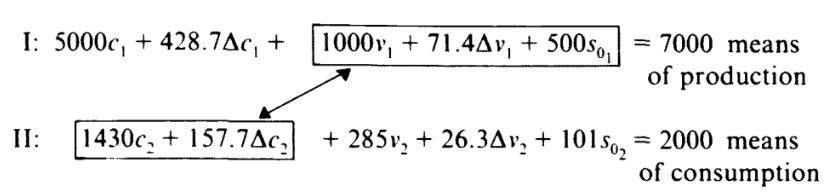
\includegraphics[scale=0.4]{rosha.jpg}
\label{fig:rosha}
\end{figure}

同样地,方框内的部分是两个部类之间相互交易的数量。第\Rnum{1} 部类为了满足其现有的
劳动力、计划增加的下一期的劳动力和资本家的消费,需要由第\Rnum{2} 部类提供1571.4单
位消费品,第\Rnum{2} 部类需要由第\Rnum{1} 部类生产的生产资料1587.7单位,用以补偿
当期消耗和计划中的不变资本的扩大所需的生产资料。这两个数字不等。“如果这是积累过
程的真实图景”,卢森堡推论说,“生产资料(不变资本)在第二年将有一个16单位的短
缺……同样地,消费资料将有16单位的过剩”,\textbf{这种不平衡将会逐期递增。}

卢森堡认为,无论是工人、资本家还是马尔萨斯主义者所说的“第三者”,都不能提供实现
剩余价值所必需的购买力。只有一个类型的消费者可以做到这一点:那些\textbf{完全外在
  于资本主义生产方式的消费者}。从而“在只由工人和资本家构成的社会里,为了积累而实
现剩余价值,就成为不可能的事情了。”存在“资本主义社会的生产能力与消费能力之间深
刻而根本的冲突。而这个冲突正是资本积累导致的,它周期性地产生危机,并驱使资本不断
扩大市场”。只有认识了这个矛盾,才有可能得出帝国主义理论。\textbf{马克思的分析无
  法揭示 “实现问题”的存在。它给人的印象是,资本积累可以不受限制地持续下去。从而
  放弃了“支持社会主义理论的最重要的客观论点……社会主义的政治行动和无产阶级阶级
  斗争的思想内容不再是经济事件的反映,社会主义不再是一种历史必然。}”《资本积累论》
的密码很容易地被解码:在批评马克思的同时,卢森堡事实上不仅批评了修正主义者,而且
还批评了考茨基和德国社会民主党正统的“马克思主义中心”。

卢森堡继续指出,在现实中,资本主义是“\textbf{通过不断地吸纳那些能够确保自身存
  在的条件来发展的}”。

卢森堡的帝国主义概念是很独特的。它不依赖于正式的殖民化,同希法亭强调垄断的增长或
银行支配地位上升也没有什么共同之处。\textbf{“资本积累的帝国主义阶段,意味着资本
  的世界竞争阶段,包含对资本落后地区——在那里资本曾经实现其剩余价值——进行工业化及
  资本主义的解放。这一阶段的特点是外债、铁道建设、革命与战争。”}卢森堡提到1900年
后向俄国、土耳其、波斯、印度、日本、中国和北非的大规模的资本输出。帝国主义的渗透
首先破坏了当地的农民经济,使得名义上独立的国家越来越依赖于欧洲的资本(该书第30章
以土耳其和埃及为例,对这个过程作了详细描述);然后,在这些迄今为止仍然落后的地区,
产生了不可抗拒的、要求独立发展资本主义的压力。这仍然是在暴力的背景下完成的:
\begin{quotation}
  经济上落后的国家及殖民地,通过战争与革命,获得资本主义自治。\textbf{革命在资本
    主义的解放过程中是必要的}。落后国家必须摆脱它们陈旧的政治组织,以及自然经济和
  简单商品经济的残余,\textbf{创造出一个适应资本主义生产目的的近代国家机器}。土耳
  其、俄国及中国的革命,即属此类。
\end{quotation}

这就引出了卢森堡引关于帝国主义的第二个定义,即帝国主义是“一个政治名词,用来表达
在争夺尚未被侵占的非资本主义环境的竞争中所进行的\textbf{资本积累}……(帝国主义)
在对非资本主义世界的侵略中,在相互竞争的资本主义国家之间发生的日益严重的冲突中,
变得愈来愈无法无天,愈来愈野蛮粗暴”。其表现之一就是\textbf{世界范围内对自由贸易
  的放弃},自由贸易“仅仅是资本主义积累史上的一个插曲”。表现之二就是\textbf{军国
  主义},《资本积累论》以对这个主题的分析结束。资本主义的每一个历史阶段都具有军国
主义的特征。军事力量被用于征服前资本主义地区,它也是“资本主义各国争夺非资本主义
文明地区的武器”。更重要的是,“\textbf{从纯粹的经济观点来看,军国主义是实现剩余
  价值的一个重要手段,它本身就是资本积累的一个领域”}。卢森堡重新回到再生产模型,
考察了作为消费者的国家产生的影响。她指出:“从工人所得中勒得的税收,在被用于军需
品生产时,就为资本主义积累提供了新的机会”,必须说明的是,卢森堡在这个问题中所作
的推理不很容易理解。

\section{对卢森堡的批判}
即使是同情罗莎·卢森堡革命左派观点的著述者,对她的经济分析也进行了猛烈的批评。
几乎没有人相信她试图证明的结论,即\textbf{在封闭的资本主义制度中积累是不可能的。}基
于同样的理由,人们对卢森堡进行一次又一次的批评,\textbf{资本家不但可以而且必须彼
  此互为客户},用于积累的那部分社会产品的需求,来自资本家意欲增加使用的不变资本和
可变资本。卢森堡对这类观点持有的反对意见,十分明显地表现在她对杜冈-巴拉诺夫斯基的
批评中,她同时也把对杜冈的批评用于反对布尔加柯夫和列宁的观点。\textbf{仅仅建立在
  资本主义需求增长基础之上,不存在对非资本主义市场的利用的积累,将意味着“人类消
  费变得越来越不重要,生产越来越成为目的本身”。}卢森堡认为,这种想法是荒谬的。但
她却错误地把持续扩大人的需求的目标,作为资本主义制度整体的目标。因为\textbf{资本
  主义制度的本质恰恰在于它的无政府性,资本主义没有也不需要一种目的,对资本主义进
  行任何形式的目的论的解释都是不恰当的。}在个别资本家层面上,卢森堡同样是错误
的。\textbf{资本家是被利润而不是被对消费增长的关注所驱动,}如果为了生产机器而不断
增加能够生产机器的机器生产是有利可图的,那就没有任何理由能够解释这种生产为什么应
当被中止。把无限制的均衡增长的可能性和它实际发生的可能性区分开来,当然是很重要的。
这里的关键问题在于投资的决定因素,但卢森堡对这一问题没有能作出详细说明。希法亭对
垄断作为一个限制支出因素的分析,有可能为这样一种投资理论提供必要的基础,但垄断在
卢森堡的思想中没有起到任何作用。

\textbf{总之,卢森堡混淆了个别资本的需要(需求的外部来源)和作为整体的资本主义制
  度的需要。}在卢森堡的分析中,还存在着三个更为严重的不相一致之处。首先,她对解释
经济危机的\textbf{比例失调论}做了猛烈的批判,因为(她认为)这一理论接受的是萨伊定
律,但她的批判据以建立的事实,她自己的解释也存在着和比例失调论类似的缺
陷。\textbf{在卢森堡提供的存在生产率提高的资本积累的算术例子中,消费品生产过剩的
  数量和生产资料供给不足的数量是相同的(如卢森堡自己承认的)。从总量上看,供给和
  需求是相等的。}第二,很难调和卢森堡对军事开支的分析和她对马尔萨斯主义者
的“\textbf{第三者}”的分析。\textbf{如果资本主义从把对工人征税所得的收入用于资助
  军备中获益,为什么用于国家闲职人员或国教方面的开支,不会产生像军备开支那样的效
  果呢?}很可能在\textbf{意识形态和政治}方面有很好的的理由,用于解释为什么资本主
义偏好于军事开支,而不是其它形式的国家活动,但卢森堡没有对这些理由进行解释。

卢森堡对帝国主义讨论的第三个也是最重要的不相一致之处,同向前资本主义市场出口的结
果有关,\textbf{如果这种出口被同等数额的进口抵消,那么出口就不会对需求水平产生任
  何直接的影响。只有出口顺差才能造成需求的净增加,但这必然意味着资本向前资本主义
  世界的输出(在不存在世界货币数量的增加时)。}卢森堡似乎没有意识到这里存在的难题。
在卢森堡的分析中,\textbf{需求不足}问题贯穿于整个资本主义发展的历史,但是资本输出
只在资本主义的最后阶段——帝国主义阶段——才变得重要起来,而且即便如此,资本输出也没
有产生像希法亭和列宁模型中所说的那种支配作用。在对资本输出的解释上,《资本积累论》
比希法亭《金融资本》的内容更少。\textbf{卢森堡的分析可以通过引入商品输出的间接影
  响来加以挽救,因为即使是在中性的贸易平衡的条件下,商品输出也会引致国内投资支出
  的增加。然而,这并不是卢森堡的观点,这再次表明卢森堡缺乏投资理论。}

此外,在卢森堡的观点中,还存在着布哈林在《帝国主义与资本积累》中指出的另外一
些不足。《帝国主义与资本积累》写于1924年,这部著作对卢森堡的理论进行了直截了当的
反驳,这部著作很可能是苏联打算对左翼反对派攻击时使用的(参见以下第十五章
)。\textbf{布哈林认为,在卢森堡的分析中,非资本主义的外围,实际上并没有受到资本
  主义的剥削,}它的功能只是实现在其它地方生产的剩余价值。此外,布哈林还认为,卢森
堡没有能够解释,为什么在资本主义努力寻求海外殖民地的同时,其本土仍然保留
着\textbf{大量的前资本主义经济形式}。布哈林还指出,卢森堡认为资本主义崩溃即将来临
的信念和她自己所持立场,在逻辑上也是不相符合的,因为世界上绝大多数人口仍然属
于“第三者”的范畴。

无论卢森堡的逻辑存在什么样的优缺点,她(完全不同于希法亭)在得出自己的结论时都是
毫不含糊的。她强调整个资本主义发展史中军事和国家力量的重要作用;强调军国主义和发
达国家之间日趋紧张的关系的经济必然性;她否定了封闭资本主义体制中稳定均衡增长的可
能性。在政治上,《资本积累论》是对德国社会民主党中的大多数人进行的激烈的、蓄意的
挑衅,因为无论是修正主义的右翼还是“马克思主义的中心”,都对消除危机的经济发展和
避免战争抱有希望。就像卢森堡在《反批判》中讲述的那样,党的机关报对《资本积累论》
持强烈的批判态度。令人惊讶的是,希法亭对《资本积累论》并没有作出反应,看起来可能
是他对经济争论失去了兴趣。考茨基迟来的反应,是以间接的方式进行的。当时,他把在
《新时代》上对这本书进行评论的任务,托付给了一个年轻的奥地利理论家——奥托·鲍威尔。
鲍威尔的文章的重要性,不仅仅体现在对卢森堡的批判上,而且也体现在他自己对马克思主
义危机理论的贡献上。

\section{奥托·鲍威尔的积累模型}

奥托·鲍威尔的分析是从对\textbf{人口增长后果}的思考开始的,他研究了在\textbf{充
  分就业情况下}资本积累必然发生的变化。这使得他能够对社会主义经济增长过程和资本主
义经济增长过程作出比较,在社会主义经济增长过程中,中央计划当局可以做出必要的调整,
而资本主义制度下生产缺乏有意识的社会调节。鲍威尔假定年人口增长率为5\%,不变资本的
使用每年以10\%的比率增长。这既包含了马克思资本有机构成不断提高的基本命题,也使得
鲍威尔能够对卢森堡提出的对再生产的分析必须考虑技术变化的挑战作出回应。“此时”的
鲍威尔,坚持剥削率保持不变,因此实际工资随着与资本有机构成提高相联系的生产率的提
高而增加。
\begin{figure}[H]
\centering
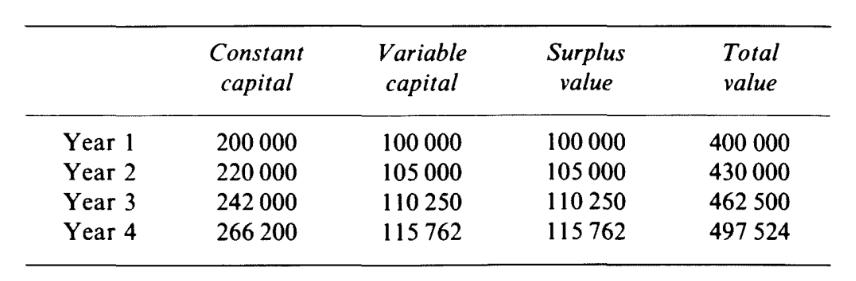
\includegraphics[scale=0.4]{bauer1.jpg}
\label{fig:bauer1}
\end{figure}

在这里,资本有机构成从第一年的2.00增加到第四年的2.30,利润率从0.333下降
到0.303(在剥削率一定的情况下,利润率必然下降)。每一年的净产出(即活劳动总量,或
者$v+m$)的增长率保持5\%不变。这是由鲍威尔的假定决定了的,由他的假定可知,可变资
本以每年5\%的比率增长,剥削率不变,因此剩余价值和可变资本有着同样的增长率。总产
出$c+v+m$以递增的比率增长,在第一年和第二年之间为7.50\%,在第三年和第四年之间
为7.57\%,更重要的是,鲍威尔称为 \textbf{“积累率”(一定程度上具有误导性)}的资
本家的储蓄倾向也在稳步增长。举例说,在第一年,100000单位总剩余价值中的25000单位被
留作积累,这使得资本家可以在第二年增加20000单位的不变资本和5000单位的可变资本。资
本家把他们收入中的25\%用于储蓄和积累。到第三年,这个比率上升到接近27\%,而且只要
不变资本比可变资本和剩余价值增长得更快,这个比率就会继续增长。

接下来,鲍威尔转向了对部类之间关系的研究。在第一年,可以表示如下:
\begin{gather*}
\Rnum{1} : 120000c_1 + 50000v_1 + 50000m_1 = 220000 \qquad 生产资料 \\
\Rnum{2}: 80000c_2 + 50000v_2 + 50000m_2 = 180000 \qquad 消费资料
\end{gather*}

如果资本家把剩余价值中的四分之一用于积累,并把它们完全投资在本部类,可以得出:
\begin{figure}[H]
\centering
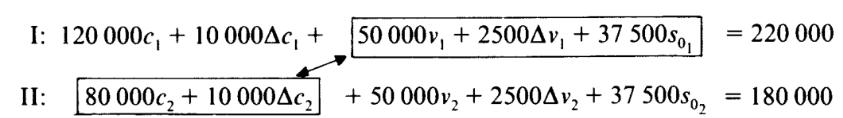
\includegraphics[scale=0.4]{bauer2.jpg}
\label{fig:bauer2}
\end{figure}
通过对方框内部分的比较,可以发现第\Rnum{1} 部类对第\Rnum{2} 部类生产的消费资料的
需求完全等于第\Rnum{2} 部类对第\Rnum{1} 部类生产的生产资料的需求(=90000)。但是
这不能建立两大部类之间的均衡,在第二年将出现如下情况:
\begin{gather*}
\Rnum{1} : 130000c_1 + 52500v_1 + 52500m_1 = 235000 \qquad 生产资料 \\
\Rnum{2}: 90000c_2 + 52500v_2 + 52500m_2 = 195000 \qquad 消费资料
\end{gather*}
生产资料产出的数量与鲍威尔假定的不变资本(是235000而不是242000)每年增加10\%所
要求的生产资料的数量相比,存在7000单位的欠缺,同时消费品的生产将会比必须的多出同
样的数量(是195000而不是188000),第\Rnum{2} 部类积累过剩,而第\Rnum{1} 部类则积累不足。

鲍威尔提供的解决方法是,第\Rnum{2} 部类的资本家把他们积累的剩余价值的一部分投资于
第\Rnum{1} 部类,增加第\Rnum{1} 部类的产出并相应地减少消费品的产出。在$10000
\Delta c_2$中, $5334$单位投资于第\Rnum{2} 部类中,剩下的 $4666$ 单位用于
第\Rnum{1} 部类的投资;同样地,$2500 \Delta v_2$中的1333单位用于第\Rnum{2} 部类,
剩余的$1167$单位转移到第\Rnum{1} 部类。第\Rnum{2} 部类的资本家可以通
过“或者\textbf{自己建立生产生产资料的工厂},或者通过\textbf{银行中介}把他们积累
的剩余价值的一部分转移到生产资料工业的资本家那里,供他们使用,或者购买生产生产资
料的公司的股份”来达到这一点。当然,第\Rnum{1} 部类的资本家的全部剩余价值被用于本
部类。

\begin{gather*}
\intertext{从而,第二年有}
\Rnum{1}: 134666c_1 + 53667v_1 + 53667m_1 = 242000 \qquad 生产资料 \\
\Rnum{2}: 85334c_2 + 51333v_2 + 51333m_2 = 188000 \qquad 消费资料 \vspace{1cm}
\intertext{第\Rnum{2} 部类的资本家拥有 4666c1+1167v1+1167m1=7000 单位的生产资料(除本部类的全部产出之外)。同样的推理,可以得出第三年的情况:}
\Rnum{1}: 151048c_1 + 57576v_1 + 57576m_1 = 266200 \qquad 生产资料 \\
\Rnum{2}: 90952c_2 + 52674v_2 + 52674m_2 = 196300 \qquad 消费资料 \vspace{1cm}
\intertext{以及第四年的情况:} 
\Rnum{1}: 169124c_1 + 61738v_1 + 61738m_1 = 292600 \qquad 生产资料 \\
\Rnum{2}: 96876c_2 + 54024v_2 + 54024m_2 = 204924 \qquad 消费资料 
\end{gather*}

与第一年相比,第\Rnum{1} 部类的资本有机构成提高了14.2\%( 从2.40到2.74),利润率下
降了9.18\%( 从0.294到0.267)。第\Rnum{2} 部类的有机构成提高了11.9\%( 从1.60增加
到1.79),利润率降低了7.01\%( 从0.385下降到0.358) 。

鲍威尔的结论就是:“不仅在第一年,而且在接下来的每一年,两个部类产出的总价值可以
在不受任何干扰的情况下出售,\textbf{总剩余价值得以实现}。因此,\textbf{卢森堡同志
  的假定——被用于积累的那部分剩余价值无法实现——是错误的}”。鲍威尔认为,并不是第一
年生产的全部剩余价值(如例子所显示的)都可以在当年得以实现有可能是正确的。如果资
本家只是在第二年开始的时候购买他们扩大生产所需的新机器,那么由 $\Delta
c_1+\Delta c_2$所代表的那部分第一年的剩余价值将只能在第二年得以实现;但它最终还是
被实现了。如果$\Delta c_1+\Delta c_2$ 所代表的商品是在资本主义世界之外的地方出售
的——卢森堡认为这是必须的——积累将受到损害,因为继续生产所需的生产资料将无从获
得。“这部分剩余产品从资本主义市场退出,将不会像卢森堡认为的那样使积累成为可能,
恰恰相反,它将使得任何积累都变得不可能”

在对卢森堡的观点做出分析后,鲍威尔转向对资本主义条件下\textbf{增长周期本质}的思考。
就这一问题来说,\textbf{必须放宽劳动力供给等于劳动力需求这一最初的假定}。如
果\textbf{可变资本的积累比劳动力的增长慢很多,将导致失业。}在这种\textbf{积累不
  足}的条件下,\textbf{实际工资下降,剥削率上升。}如果\textbf{在资本家的储蓄倾向
  既定的情况下,积累率将增大。最后到达的一点就是,可变资本的增长超过劳动人口的增
  长。然而,随后发生的是暂时性的积累过剩。}随着失业后备军的减少,实际工资再一次上
升,剥削率下降,这个过程一致持续到不仅利润率而且生产出来的剩余价值的绝对数量也开
始下降。马克思描述的“绝对生产过剩”导致一次重大的经济危机,在危机中积累受到严重
的限制,失业率上升,实际工资下降,利润率再次得到恢复。“繁荣、危机和萧条的周而复
始,经验地表现了一个事实:\textbf{资本主义生产方式自动地产生积累过剩和积累不足,
  资本积累反复地根据人口的增长进行调整}”。

一旦从\textbf{国际范围}内考虑问题,\textbf{国内人口的增长}就不再是一个关键因素。
积累过剩可能会因其它地方存在积累不足而在一些地区持续发生。
\begin{quotation}
  经常出现\textbf{积累过剩}的国家,把它们每年积累的剩余价值的很大一部分\textbf{投
    资到国外},而且这部分剩余价值越来越大。例如:法国和英国。经常出现\textbf{积累
    不足}的国家\textbf{引进国外资本并把劳动力输出}到国外。如东欧的农业家。在一国
  内部生产性资本的扩张总是受限于可以获得的劳动力。
\end{quotation}

这就凸显了卢森堡错误的帝国主义理论中的真理内核。\textbf{尽管积累在封闭的资本
  主义制度中是可能的,但它也受到了限制。帝国主义有助于放松这些限制,}它不仅通过扩
张能够招募到新劳动力的控制区,而且也通过获取原材料、刺激有机构成超过平均水平的产
业的发展,以及在经济危机期间,为“庞大数量的商品”提供市场来放松这些限制。

鲍威尔否认他的分析是对帝国主义的辩护:
\begin{quotation}
  因为在资本的辩护者想要证明积累——消费能力随着生产的扩大而自动地上升!——不受限制
  的本质时,我们揭示了积累受到的限制。在资本的辩护者想要证明普遍危机的不可能性时,
  我们说明了\textbf{积累的规律只能通过普遍的危机发挥作用},说明了危机造成的失业、
  工资的减少、大众苦难的增加、大多数工人日益增加的痛苦和愤慨。
\end{quotation}

从而,资本主义确实给自己带来毁灭,即使不是以卢森堡所假定的那种方式进行:
\begin{quotation}
  如果资本主义的扩张是可能的,它将会因军备竞赛、越来越多的压迫性税收、灾难性的战
  争而引起工人大众的愤怒。如果它的扩张被阻止了,对积累的限制就会加剧,危机变的更
  加频繁,持续的时间更长,更具破坏性……\textbf{资本主义将不会因实现剩余价值的机
    械的不可能性而崩溃,它将被它所激起的群众的愤怒所击败。}并不是只有当最后的一个
  农民和最后的一个小资产阶级都变成雇佣工人,从而不再提供一个实现剩余价值的市场的
  时候,资本主义才瓦解:被资本主义生产方式本身教育、联合和组织起来的日益壮大的工
  人阶级愈来愈强烈的愤怒,将会早得多地把它击溃。
\end{quotation}

\section{卢森堡的《反批判》}
鲍威尔的增长模型无疑是1914年之前由马克思主义经济学家尝试进行的\textbf{最成熟的宏
  观动态分析},它与现代\textbf{哈罗德—多马理论}之间的密切联系,直到最近才被完全理
解。鲍威尔文章的目的是为了驳斥卢森堡的崩溃理论,并说明\textbf{在封闭的资本主义经
  济中稳定的均衡增长是可能的}。尽管他对《资本积累论》的批评是有力的——这本来就是一
个很容易达到的目标,但是鲍威尔自己的模型也未能经受住更加细致的审查。早
在1929年,\textbf{亨利克·格罗斯曼}就证明了鲍威尔数值例子中所确定的增长路
径,\textbf{不可能无限期地持续下去},这已经被现代数学分析所证实。在经过32年的生产
周期后,\textbf{经济将会耗尽它用以维持给定的积累率提供资助的剩余价值}。这是鲍威尔
不变资本以两倍于可变资本的速度增加,剥削率保持不变的假设的必然结果。从代数上
看,m1和m2上升的太慢以至于无法满足模型所要求的 $\Delta c_1+\Delta c_2$ 的持续增加,
积累的过程无法一直继续下去。从技术上看,鲍威尔的模型过于武断。稳定增长只有在鲍威
尔提出的限定条件中,至少有一个被放松的情况下才是可能的。一个明显的选择是允
许\textbf{剥削率上升},从而可以增加用于积累的剩余价值的增长率。然而,即使在这种情
况下,\textbf{也不存在}充分的灵活性能够保证稳定增长的可能性,\textbf{确保这种可能
  性的最确定的方法是保持资本有机构成不变}。在不考虑鲍威尔本来意图的情况下,他的模
型是一种和技术变革过程中的\textbf{利润率下降趋势紧密联系在一起}(在任何简单的意义
上都\textbf{不是引起})的\textbf{资本主义经济崩溃理论}。

然而,这种判断完全不会损害鲍威尔危机理论的声誉,他的危机理论只能用它自身的优点来
加以评价。\textbf{积累不足时期和积累过度时期交替出现的概念有着直观的吸引力,}而且
它的确引起了许多后来的马克思主义经济学家的注意,这在很大程度上是因为它在避免了比
例失调、消费不足和利润率下降理论中的许多固有困难的同时,提供了对\textbf{周期性波
  动}的解释。但是,鲍威尔的理论也存在一个重大的缺陷,因为\textbf{它没有考虑生产能
  力利用率的波动。萧条时期总是产生严重的产能过剩,因为总需求不足以实现}经济中的生
产潜力得到充分发挥时生产出来的\textbf{全部剩余价值}。正是由于这个原因,马克
思\textbf{坚持把危机和实现问题紧密的联系在一起}是正确的。在文章的开始部分,鲍威尔
的确提到了资本主义社会生产能力的持续增加和资本主义消费能力逐渐缩小之间的矛盾,但
是,这种考茨基式的暗示并没有很好地加以深入展开。因此,鲍威尔对经济危机的解释是很
不完整的。

这些批评中,很少有哪个是由卢森堡在她那明显充满愤怒情绪的《反批判》中提出的,她对
鲍威尔提出的很多反对意见是\textbf{不着边际}的。她指责说人口变化不是资本积累的真正
基础,积累可以在人口保持稳定的情况下进行(就像当时的法国那样);\textbf{积累决定
  了人口增长率而不是相反}。 卢森堡把鲍威尔对两部类之间比例失调的分析驳斥为“纯粹
的欺骗”,并否认第\Rnum{2} 部类的资本家会像鲍威尔设想的那样,购买保持均衡增长所需
的4666单位的生产资料。这明显是错误的,卢森堡本来可以通过对平衡增长的可能是如何转
化为现实的进行提问,通过对直到\textbf{第二年进行购买之前一直保有第一年生产的商品
  存货的资本家的资金来源}进行探究,表现的更好。卢森堡认为鲍威尔模型中的\textbf{剥
  削率应当上升而不是保持不变},是建立在坚实的基础之上的,但即使是在这里,她也因坚
持在剥削率保持不变的情况下,“所有的技术进步只是为了工人的利益”而损害了自己的理
论。

虽然反对战争,但考茨基主义者拒绝接受通过革命推翻资本主义是通向和平的唯一的道路的
观点,他们认为能够使资产阶级相信帝国主义的终结是符合他们的利益的。“无产阶级和资
本之间为解决它们的世界历史矛盾而进行的最后的对抗,变成无产阶级和资产阶级之间
为‘\textbf{缓和}’资本主义国家之间的帝国主义矛盾而进行的\textbf{历史性妥协的乌托
  邦}”。正是因为卢森堡认为鲍威尔持有这样的立场,才对他的政治经济学如此敌视。


\section{考茨基对帝国主义的第二次思考}
考茨基1914- 1915年的文章和卢森堡的《反批判》,是最后的也是重要的论述帝国主义理论
的德国文献。

直到文章的最后部分,考茨基才开始和卢森堡(没有提到她的名字)背道而驰。在这里,考
茨基否认了帝国主义必然是资本主义的最后阶段。持续获得原材料和资本投资的出路,对资
本主义体系的生存是必不可少的。但是\textbf{军国主义和战争并不必然符合除武器生产商
  之外整个统治阶级的利益}。“今天,每一个有远见的资本家都会向他的同僚大声呼喊:全
世界的资本家,联合起来。”资本家们受到殖民地解放运动和国内工人阶级对帝国主义强加
给他们的财政负担的反抗带来的威胁,同时资本积累也因沉重的利税而处于极度的危险之中。
从而帝国主义在自掘坟墓……从纯粹经济学的观点来看,资本主义不是不可能再经历一个新
的阶段,即\textbf{卡特尔政策在外交政策上取得胜利的超帝国主义的阶段}。对于超帝国主
义,我们当然必须像对付帝国主义那样地同它作坚决的斗争,虽然它所带来的危险是在另一
方面,而不是在军备竞赛和威胁世界和平方面。

考茨基承认战争是可能的。因此,“\textbf{帝国主义的神圣同盟}”只能出现在全球冲
突终结的时候。任何世界战争持续的时间越长,这种同盟就越有可能产生。

作为事后诸葛亮,人们很容易对考茨基关于战争可能避免的主张嗤之以鼻。然而,在考茨
基写作的时候,存在着使人相信国际紧张局势正在缓和的理由。

战争爆发几个月后,考茨基重新回到这个论题,对修正主义者伦施和库诺进行了批评,他们
披着卢森堡的外衣,认为正是因为帝国主义是资本主义发展的一个必要阶段,所以社会民主
党对帝国主义的反对是无效的、反动的。考茨基认为这是对希法亭《金融资本》的误解,在
《金融资本》中,\textbf{帝国主义被认为是一种政策而不是一个独立的阶段}。因此,有可
能存在其它的政策选择,可以想象,\textbf{当前造成战争的政策将会被新的政策取代,这
  种新政策允许“国际上联合在一起的金融资本对世界进行共同的剥削”。这种超帝国主义
  政策将会削弱资本主义制度道德破产的趋势,预示着“资本主义的新希望和新期望的时
  代”。一切取决于战争的结果。}

\part{俄国到1917年的贡献}
\label{part:russia}

\chapter{俄国马克思主义的遗产}

\section{引言}
马克思留给俄国的遗产与留给德国社会主义者的遗产迥然不同。尽管他们能够接触到的马克
思的著作在本质上是相同的,但在\textbf{俄国资本主义不发达和沙皇专制的背景下},这些
著作中的有关内容显得较为晦涩。而且马克思关于俄国的具体观点往往没有什么充分的根据,
同他关于历史发展的整体理论毫不相干。

\section{俄国专制主义的本质}
以下将要证明的是,俄国作为欧洲持续时间最长的专制国家,在19世纪中叶仍然十分稳固。
沙皇国家中央集权官僚机构对社会统治的程度,是较早时期西欧专制国家无法比拟的。国家
是主要的土地所有者,拥有大部分的非农业经济部门。与幅员辽阔的领土相匹配,帝国控制
着一支庞大的军队,以及一整套对内镇压的国家机器。宗教不独立,教育机构的自治也微乎
其微。帝国的意识形态并不复杂,它打得旗号是“权威、正统和民族性”。这一意识形态的
谱系是清晰的、绝对的,因为沙皇专制国家没有经历过类似于在德国和奥匈帝国那样的改革。
俄罗斯帝国\textbf{完全不具备代议制议会、男性普选权和公民权}这些德意志帝
国19世纪70年代所具有的特征,甚至到了20世纪也依然如此。沙皇专制国家\textbf{经受住
  了}资产阶级革命的高潮和随之而来的拿破仑扩张的考验。事实上,它进行了反击,这种反
击不仅在最终击败拿破仑时发挥了作用,而且(自18世纪晚期以来)为了镇压革命和支持反
动势力而准确地打入西方。


俄国\textbf{“利维坦”(Leviathan)的阶级特征}是一个复杂的问题。现代历史学家往往
强调国家的独立和国家利益的至高无上。实际上,这种观点在马克思把俄国称作“半亚细
亚”国家时也有所体现。在革命之前,俄国马克思主义者也持这种观点。但是,马克思探讨
阶级与国家关系的理论蕴涵着复杂的视角。尽管现实是充满矛盾的,但这些矛盾并不是那么
的明显,人们不太可能就追求阶级利益所需的必要条件使达成共识。从而,任何一个阶级国
家都必定会获得某种程度的自治。

至19世纪中叶,经济上占统治地位的阶级是世袭贵族,他们的土地所有权是稳固的:
\begin{quotation}
  在大约100000个贵族地主中,接近50000个地主拥有不到270公顷地产。另外一半的贵
  族地主,却在10亿公顷贵族土地中占有97\%,而且在俄国的欧洲部分,这些面积超过了所
  有私人拥有的土地50\%多。给人印象更深的是,极少的(10\%)农业贵族拥有了2700公顷
  的土地,其比例占所有不动产土地中的75\%。甚至155个超级权贵,他们的不动产平均
  达270000公顷,其比例占所有贵族土地的33\%。
\end{quotation}
值得注意的是,国家机器与贵族结构的融合。在尼古拉一世统治下,
\begin{quotation}
  对应于国家官僚机构的级别,在贵族阶级内部形成了一种封建等级制。反之,凡在国
  家机构中占据确定位置的人,也被授予相应的贵族等级,在一定级别之上的等级为世袭等
  级。这样,一直到1917年,贵族头衔和特权,通过政治体制同各种级别的行政职能联系在
  一起。
\end{quotation}

这种相对单纯的封建专制主义形式,意味着支撑它的经济基础是极其落后的。1861年俄国的
人均国民收入不到德国、法国和意大利的一半,不及英国的1/4和美国的1/6。婴儿死亡率和
文盲率明显是欧洲最高的。

\textbf{国外的军事压力与国内的农民反抗和叛乱}这两股并行的历史力量,塑造了俄国社会,
这也是在稍后一个时期造成它分裂的力量。两种力量最初都起到了加强中央集权维护贵族安
全的作用,“\textbf{一方所需要的政治忠诚,是用满足另一方所要求的世袭农奴制换取
  的。}”这一过程(农奴制)开始于15世纪的相对较小的莫斯科公国伊凡三世时期,尽管与
所有的成长中的专制主义国家一样,专制主义在俄国经历了几番潮起潮落,但是,在18世纪
初彼得大帝统治时期,农奴制在更大范围内得到了巩固。独立的贵族权力受到了压制,通过
要求贵族承担普遍的服役义务,提高了贵族的官僚职能,同时也巩固了他们对农民的经济剥
削。农民流动受到限制,农奴制进一步得到强化,他们的反叛遭到镇压。城镇自治被粉碎了,
一个地理上不断扩张的帝国,为中央权力的高度集中创造了条件。

然而,随着资本主义工业化在西方世界的扩张,这一体制遭受的压力越来越大。
其\textbf{脆弱性},在1856年克里米亚战争失败中暴露无遗,此后,这个专制国家开始了更
大规模的现代化。19世纪60年代农奴制的废除和19世纪80年代以后凸现的对快速工业化的扶
植,是这一现代化过程中两个最显著的变化。前者为先前的工业化的加速发展,提供了更大
的活力。劳动力从农村向城镇的流动更为方便,国家和贵族之间分享农业剩余份额的竞争减
弱了。此时,国家面临的约束更少了,\textbf{从农村获取资源为雄心勃勃的工业化提供资
  金的能力更强了}。

到1914年,俄国已经成为世界第五大工业国,之前30年的增长超过了世界上其他任何地区。
一个高度发达的资本主义工业国在旧制度内得以建立。与此相伴的是,它造就了自己的掘墓
人——一个人数不多但高度集中的\textbf{城市无产阶级},这一阶级与农民有着千丝万缕的联
系,\textbf{对农民剥削的加重是这一过程得以完成的主要方式。}

\section{马克思和恩格斯论俄国}
这些不是马克思和恩格斯在19世纪40年代看到的俄国现实。很大程度上,他们所面对的只
是更为简单的专制政体。此外,19世纪70年代之前,他们的主要兴趣不在于帝国的内部条件
上,而在于俄罗斯帝国对外部产生的冲击上。

马克思和恩格斯论述亚细亚社会内部结构,即他们认为的同俄国有关的社会结构的更加深思
熟虑的著作,也是不充分的。事实上,\textbf{亚细亚生产方式}这一概念,现在被认为具
有\textbf{内在的不一致性},在把这一概念应用于经验研究时,时有不确切之处。就俄国个
案来说,这种情况并不是十分明显,这是因为人们经常通过为这个术语添加前缀而改变它的
限定条件。不管怎样,把沙皇帝国称为“\textbf{半亚细亚社会}”,只会使人更加困惑。在
这里,如同得到了一个加权平均的概念,但只对构成这一概念的某一单一要素作了详细说明,
而未对构成它的所有要素的权重进行设定。此外,马克思对俄国具有亚细亚社会性质的解释,
有时候显得有点过于唯心主义。马克思认为19世纪50年代之前,俄国没有“国内史”的观点
近乎荒谬。

恩格斯认为的沙皇政府在对内政策方面“不能理性行事”的观点,从根本上\textbf{低估了
  沙皇政府的自我调整能力}。

尽管如此,马克思和恩格斯通过把俄国与亚细亚生产方式联系起来,\textbf{强调俄国的非
  欧洲特征},这对后来的俄国马克思主义影响至深。在普列汉诺夫的理论发展中,他逐渐强
调俄国历史的非西方的特征(参见以下第八章),并且反对列宁的“\textbf{无产阶级和农
  民民主专政}”理论,因为实现这种民主专政,就\textbf{无法根除俄国农业秩序中的亚细
  亚社会的特征}(参见以下第十一章)。列宁本人也无法前后一致地提出一个有关俄国阶级
本质的理论,他在几种观点之间徘徊不定,\textbf{先是强调俄国的亚细亚属性,继而强调
  它的封建性,最后是它的资产阶级属性。}孟什维克则专注于在俄国复制他们认为的西欧政
治历史一直遵循的发展道路。托洛茨基最初形成的“不断革命论”的信念就在
于:\textbf{在俄国,国家创造了符合它自身利益的阶级等级。}在斯大林专制统治时期,作
为对“\textbf{一国社会主义}”意识形态进行广泛辨护的组成部分,\textbf{斯大林否定了
  亚细亚社会形态这一概念;这一概念和苏联现实之间存在的明显的相似性,使他感到不安
  (参见以下第十五章)。}

马克思关于1848年德国革命的著作,也以各种不同的方式影响着俄国马克思主义者。由于德
国经济的落后,马克思\textbf{起先承认}资产阶级领导革命是合适的,但很快他
就\textbf{开始批判}资产阶级的保守性。马克思最终转向了另一个立场,
即\textbf{强调}无产阶级和农民在激化革命方面发挥重要的作用。马克思预期的以这样的战
略成功的革命,到底是什么类型的革命,这并不太清楚。对1848年革命的研究,最终并没有
得出什么结论。马克思\textbf{随后集中关注的是发达资本主义国家背景下的无产阶级革命}。
不过,他确实从1848年革命中得出了某种具有一般性的经验教训,这反映在\textbf{德国马
  克思主义者在任何情况下都坚持无产阶级政党要保持自己的独立性上。}鉴于沙皇长期的专
制统治和俄国社会形态的相对落后,要求俄国马克思主义者\textbf{超越这一事实},并赋予
马克思对1848年革命进行的论述更加重要的意义是合理的。因此,普列汉诺夫不仅强调社会
民主党必须保持它的独立性,而且强调它要取得资产阶级民主革命的领导权(参见以下第八
章)。1905年之后,列宁在此基础上进一步提出,\textbf{农民的支持是必不可少的},在资
产阶级革命中无产阶级必将同资产阶级发生冲突(参见以下第十一章)。最重要的是,托洛
茨基主张,马克思有关1848年革命的观点,含蓄地表达了革命变革的一种新范式,在俄国存
在的由农民支持的无产阶级掌握革命领导权,意味着\textbf{资产阶级革命将迅速地进入社
  会主义革命阶段}(参见以下第十二章)。

马克思和恩格斯对俄国分析存在的缺陷,部分原因是由他们主要关注其他问题造成的。但是,
即使当马克思最终开始深入研究俄国的社会经济结构时,他的结论仍然具有“例外论”的特
征。他认真地考察了\textbf{以农民为基础的非资本主义发展的可能性},这种发
展\textbf{无需借助无产阶级的革命力量,最终达到社会主义。}在这方面,他深
受\textbf{俄国民粹主义}的影响。\textbf{民粹主义}是一场包含了多方面主题的运动,它
在整个19世纪后半叶主宰了整个知识分子阶层的思想。事实上,直到20世纪30年代,斯大林
的\textbf{集体化运动}才真正终结了民粹主义对俄国知识分子的影响。民粹主义也是一种中
介,马克思主义通过它开始在俄国发生影响,这一影响的核心部分就是马克思的经济学。

\section{俄国的民粹主义}

村社,在某些方面类似于原始共产主义。它的根本特征在于\textbf{公社土地的公有制},
土地在家庭之间定期进行平均再分配,以确保所有人维持生存。带状土地和轮作制农业使个
体劳动成为可能,但这要求农村公社进行\textbf{集中管理}。农民对领主费用和国家税收承
担连带责任,强化了这种特征,结果村社掌握并行使权力,村社权力约束了农民的个人主
义。19世纪60年代取消农奴制之前,农业经济自身及其同地主和国家之间的联系,是极
其“自然的”,几乎不存在货币交换。

因此,农村公社在多大程度上开始解体,农民在多大程度上开始出现社会分化,这些问题
在19世纪末成为俄国社会主义者争论不休的话题。事实上,即使是现在,这些话题仍颇具争
议。然而,农村公社以及维持其长期运行的惯例,并没有随着农奴制的消失而消失,这却是
一个不争的事实,而且非资本主义关系继续占据支配地位。这正是俄国农业极其落后、传统
残余对农民的意识仍在产生强大影响的部分原因。

这也为俄国的斯拉夫人捍卫旧政体提供了经济支柱。通常认为,村社阻止了西方常见的有害
的、堕落的个人主义的发展,因而也抑制了自由主义、无产阶级和社会主义的发展。相
反,\textbf{无论是否意识到,村社也把农民束缚于专制沙皇和东正教居于顶端的旧秩序
  中。}从而,俄罗斯帝国作为一个统一的国家,能够进一步地开拓疆域,能够“解放”南欧
的斯拉夫人,并与西欧的扩张主义相抗衡。

\textbf{对民粹主义者来说,正是村社提供了进入社会主义新社会的希望。}在他们的蓝图中,
村社关系阻止了西方个人主义的发展,奠定了(在他们看来的)现代社会主义蓬勃发展的基
础。从而,俄国在自身的发展过程中,\textbf{能够跨越资本主义发展阶段,通过对政治结
  构的适当改造,直接走上集体主义道路。}正是农业体制落后的社会本质,使得俄国的发展
可以是\textbf{直线型的——古老的俄国能够成为新俄国的基础}。资本主义发展的辩证法,既
不必要、也不值得期待。当然,民粹主义者认识到,村社并不是一种最优的社会制度。宗法
关系、近乎普遍的无知和经济的不发达如此明显,使得民粹主义的观点很难在具有浓厚的人
道主义精神、深受西方思想熏陶的知识分子阶层中流行。但是,民粹主义者相信,随着经济
的发展,沿着社会主义道路展开的启蒙运动,将会使这些不利因素逐渐消失。

马克思的经济学容易被融入到民粹主义的框架中。19世纪80年代之前,马克思的经济学主要
发挥了告诫功能:如果资本主义生产关系在俄国占据支配地位,那将会发生什么事情?换言
之,\textbf{俄国的广大民众将不得不经历伴随着资本主义的“运动规律”而来的所有的恐
  怖}。《资本论》对这些恐怖状况的描述,对它们和资本主义本质存在的紧密联系的分析,
对几乎所有的民粹主义思想家都产生了广泛而深远的影响。在马克思对民粹主义产生影响的
过程中,民粹主义也对马克思产生了影响。马克思没有试图去哄骗他的俄国读者继续接受
他30年来竭力阐述的观点,而是沿着采纳民粹主义思想的方向前进。

\section{“晚年马克思”}
马克思在赫尔岑的著作中初步接触到民粹主义思想,民粹主义并没有给马克思留下什么
好印象。这更多的是由于民粹主义者解释问题时表现出来的\textbf{斯拉夫气质}而不是他们
的内容造成的。无论是马克思还是恩格斯,他们从不掩饰对民粹主义作为俄国沙文主义的一
个变种的蔑视,尽管在他们看来,民粹主义可能更为仁慈。但是,后来的民粹主义者放弃了
斯拉夫主题,加之一系列其它因素的影响,19世纪70年代,马克思对民粹主义理解的视角发
生了转变。埃德蒙·威尔逊将这种转变描述为充满才智的头脑迸发出的“\textbf{最后的重要
  的火花}”,马克思这时\textbf{转变}了立场,承认俄国民粹主义者的奋斗目标是可能
的。20世纪的新民粹主义者坚持认为,在作出这种转变的同时,马克思本人也为“晚年马克
思”奠定了基础,新民粹主义者要求一并注意“青年马克思”和“成熟马克思”,“青年马
克思”探讨的主题极大地影响了一战后的西方马克思主义;“成熟马克思”的思想成为第二
国际的思想内核。

车尔尼雪夫斯基的经济学给马克思留下了深刻的印象,\textbf{车尔尼雪夫斯基强调俄国与
  西方的不平衡发展,认为俄国有可能复制西方的成就,而无需付出后者那种惊人的代价。}摩
尔根的人类学改变了马克思有关原始公社形式地位的观点,很可能促使马克思对俄国社会进
行了广泛深入的研究。

然而,“晚年马克思”并没有撰写出可与《1844年经济学哲学手稿》、更不要说与《资本
论》相媲美的著作。马克思只有一些晦涩的评论,散见于他为早期著作所写的附注中,以及
回答俄国一些向马克思征询对他们所关注问题的看法的信件中,事实上,这些信件的草稿有
些从来就没有发出。马克思有关俄国的观点,如果不借助现代的想象力加以扩展,所有这些
观点无论如何也难以构建成一个“体系”。这些观点,至多是一种梗概式的立场描述,这些
立场涉及的主题从未被详细地加以说明,也与早期的分析没有什么联系。

马克思个人对民粹主义的兴趣,最早出现在1877年他对民粹主义者米哈伊洛夫斯基关于《资
本论》的充满敌意的评论的回应中:
\begin{quotation}
  为了能够对当代俄国的经济发展作出准确的判断,我学习了俄文,后来又在许多年内
  研究了和这个问题有关的官方发表的和其他方面发表的资料。我得到了这样一个结论:如
  果俄国继续走它在1861年所开始走的道路,那它将会失去当时历史所能提供给一个民族的
  最好的机会,而遭受资本主义制度所带来的一切灾难性的波折。(《马克思恩格斯文集》第3卷,人民出版社2009年版,第464页。)
\end{quotation}

马克思坚持认为,《资本论》第一卷中\textbf{对原始积累的论述只适用于西
  欧},\textbf{否认}它是“一般发展道路的历史哲学理论,一切民族,不管它们所处的历
史环境如何,都注定要走这条道路”。它对俄国的适用性只表现在:
\begin{quotation}
  假如俄国想要遵照西欧各国的先例成为一个资本主义国家——它最近几年已经在这方面费了
  很大的精力——,它不先把很大一部分农民变成无产者就达不到这个目的;而它一旦倒进资
  本主义制度的怀抱,它就会和尘世间的其他民族一样地受到那些铁面无情的规律的支配。
  (《马克思恩格斯文集》第3卷,人民出版社2009年版,第466页。1857-1858年的《政治经
  济学批判大纲》表明马克思的前资本主义社会的发展方案并非线性的。)
\end{quotation}

1881年,在回复维拉·查苏利奇要求马克思提供关于“俄国农村公社可能的命运”的信件中,
马克思再次重申了这一立场。尽管马克思断言“这种农村公社是俄国社会新生的支点”,但
他又说“可是要使它能发挥这种作用,首先必须排除从各方面向它袭来的\textbf{破坏性影
  响},然后\textbf{保证它具备自然发展的正常条件}”。这种回复,明显地引发了马克思
更多的思考。至少有4封信件的草稿为人所知。正是这些信件充实了马克思论点的关键部分,
马克思认为,\textbf{农村公社把集体主义和个人主义结合到生产关系中。土地归集体所有,
  但劳动过程是个体式的,可转让的财产受制于私人交换。两种不同的发展都是可能的,}这
取决于哪一种要素占主导地位。沿着沙皇俄国的现代化启动的当前的道路继续前行,最终将
导致公社的消失和资本主义关系的产生。但是,这个过程并不是不可避免的。如果它因民粹
主义者的革命而中断,将有可能在公社的基础上建成共产主义,使西方资本主义的积极成果
融入社会主义者对公社进行的重组中。

在致查苏利奇的信件的草稿中,马克思没有再提及,\textbf{民粹主义发展道路的实现取决
  于西方发达国家的无产阶级革命}。然而,在为1882年俄文版《共产党宣言》所写的序言中,
他又加入了这一限定条件。这可能体现了恩格斯的影响,恩格斯是序言的共同作者,恩格斯
事实上起草了这一序言。同马克思相比,恩格斯有关“晚年马克思”主题的著述,无疑更加
强调西方政治领袖对实现民粹主义理想是必不可少的。也有证据表明,恩格斯从未认真地思
考过这一前景,即使是在马克思逝世之前。 1883年之后,恩格斯的有关这一立场的观点得到
进一步强化。恩格斯的怀疑论也反应在20世纪俄国马克思主义者的观点中。虽然他们有时候
承认俄国有可能避免经过成熟的资本主义的发展阶段,但是他们总是指出出现这种情况需要
国际革命。\textbf{“一国社会主义”学说是20世纪20年代的产物,1917年之后欧洲革命的
  失败是它形成的原因之一}(参见以下第十五章)。

对“晚年马克思”思想重要性的任何评价,都必须面对这种思想与早期著作中的思想的不一
致之处,而且必须考虑早期思想在19世纪70年代对马克思的影响。显然,晚年马克思的观点
与他早期的大量著述中反映出来的观点并不一致:马克思明显抛弃了在《资本论》中阐述
的\textbf{普遍适用的工业化的“自然法则”}。从他最早期著作开始,\textbf{一直存在的
  一个主题,即对无产阶级独自作为共产主义的代理人的效果的分析,现在加入了社会主义
  可以通过同知识分子和农民的结盟得以实现的新内容。}很显然,马克思早年许多有关农村
生活愚昧、农民的不开化以及缺乏政治上的可靠性的污蔑,适用的范围更为有限了。从19世
纪80年代开始,对西方帝国主义应当在更加相对的意义上加以认识,比如,\textbf{就西方
  帝国主义对印度的影响,马克思一方面谴责了它的残忍性,另一方面也欢呼其进步性。}

无论如何,民粹主义的目标都是不可能实现的。任何试图在村社的基础上实现的社会主
义,都将导致\textbf{独裁主义}。\textbf{领袖与群众之间的距离、劳动生产率的欠发达,
  都意味着不可能以民主的组织方式转向社会主义。}即使在农民中广泛存在着一定程度的巴
枯宁主义情绪,为了充分实现生产的社会化需要瓦解传统公社的生产关系,这势必要求解除
那些社会化的权力。那么,在避免经历阶级形成的沧桑巨变下,拿什么拯救统治精英?在马
克思逝世那一年,在青年马克思的马克思主义的指导下,普列汉诺夫明确地表达了这些用来
反对民粹主义的观点。“晚年马克思”当然没有为反对民粹主义的观点提供理论基础。

\section{结论}
因此,马克思留给俄国追随者的遗产,比留给德国同志的遗产更加复杂。德国马克思主义
者对马克思的亚细亚社会概念的理论兴趣有限。然而,对俄国马克思主义者来说,这个概念
表明他们面对的情况与欧洲完全不同。这突出了如下事实:\textbf{俄国资本主义的发展具
  有自己独特的特征,合适的革命策略需要采取特定的斗争形式},例如,马克思在评
价1848年德国革命时所概述的那些斗争形式。\textbf{即使是马克思成熟著作的核心部
  分——资本主义生产方式的运行规律——与俄国的相关性也是存在争议的。俄国不必等待修正
  主义的争论吞噬他们的各个阶层。从一开始修正主义就存在,而且明显得到了马克思自己
  的支持。}

\textbf{自1903年起},俄国社会民主党内部出现了新的裂缝。这时候,俄国社会民主党分为
孟什维克和布尔什维克两派。两派的分歧是由\textbf{党应当采取何种组织形式}的争议引起
的,但是后来把经济理论问题也牵涉进来(参见以下第8章和第11章)。如果不存在争议,也
就不会有俄国马克思主义的两派。\textbf{就政治经济学来说,最重要的是托洛斯基的不平
  衡和综合发展理论(参见第十二章)。}在\textbf{1917年之前},托洛茨基及其同仁接受
了\textbf{孟什维克的政党组织的观点},但是,他们的\textbf{激进主义}使得他们更像布
尔什维克的主要理论家列宁和布哈林(参见以下第十一章、第十二和第十三章)。1914年第
二国际解体后,俄国马克思主义的内部差异变得更加明显,不同团体进行了重组。1917年,
托洛茨基和列宁联合起来,但是大量的孟什维克和一些布尔什维克反对十月革命,因
为\textbf{他们认为冒险主义不符合正统马克思主义的原则}。(参见以下第八章和第十三
章)。

同时,由于马克思把俄国描述为欧洲的\textbf{反动堡垒},这使得俄国革命被认为是具有头
等重要性的国际事件。结果,\textbf{改良主义变成了一支微弱的力量,而革命强硬传统成
  为一支更为强大的潮流,}马克思本人体现出的这种特征,在说德语的理论家中只
有\textbf{罗莎·卢森堡}保持着这种传统。早期的经济理论的发展,清楚地说明了革命实践
的优先性。为了制定有效的革命战略,人们很少关注价值理论和资本主义危机理论,而把更
多的注意力放在理解俄国经济发展的本质上。

\chapter{普列汉诺夫的政治经济学}

\section{引言}
1880年左右,“晚年马克思”逐渐形成,年轻的普列汉诺夫却正在向着相反的方向发展。他
同自己过去的民粹主义决裂,接受了包含成熟马克思的核心主题在内的马克思主义,由此开
始了他的思想在俄国革命界逐渐占据统治地位的过程。他知道自己有关俄国的观点与马克思
的不同,而且在马克思逝世后的许多年,他很少得到恩格斯或其他马克思主义领袖的鼓励。
这些事实表明了他在知识方面的自信。……\textbf{孟什维主义}牢固地建立在普列汉诺夫的
马克思主义基础之上,没有任何一个孟什维主义理论家在学术地位上可以与他相比。……即
使在1905年普列汉诺夫同布尔什维克因“革命的算术”问题决裂之后,列宁仍然视自己为普
列汉诺夫革命的“代数学”的支持者(参见以下第十一章)。十月革命的胜利无法证明列宁
对普列汉诺夫哲学著作的赞赏,十月革命的理论原理与普列汉诺夫的理论格格不入(参见以
下第十三章)。在苏联,普列汉诺夫的著作,在官方认可的合法的基本的理论著作中,占据
突出的位置。

普列汉诺夫的马克思主义理论体系源自同革命的民粹主义的论战,他整个一生不断卷入各
种各样的理论争论。然而,他的纲领本身却表现出异乎寻常的恒定品性。实际上,普列汉诺
夫从来没有向他的论敌做过任何妥协。\textbf{俄国的资本主义将会继续沿着西方的道路发
  展,步入社会主义,要求马克思主义者首先集中关注资产阶级民主革命的实现问题。}

\section{普列汉诺夫体系,第二国际的正统和俄国马克思主义}
普列汉诺夫创造了一个术语——“\textbf{辩证唯物主义}”,用来界定马克思主义的本质。
在第二国际的知识分子中,他是马克思主义最博学的倡导者。他有关哲学思想的兴趣和知识
首屈一指。

普列汉诺夫的著作具有的这些特征,使得他的马克思主义被描述为一种具有极其僵化形式的
马克思主义,而且这主要还是一种\textbf{依赖于恩格斯晚期著作的马克思主义}(现在所知,
在始终不渝地支持这种马克思主义的人中,并不包括马克思),他的马克思主义也被描述为
一种能够十分便利地融入斯大林主义的意识形态中去的教条主义。毫无疑问,普列汉诺夫紧
紧地追随恩格斯,他无法认识到在恩格斯对黑格尔的分析中,以及把辩证法扩展到自然界时
存在的难题。普列汉诺夫也错误地认为,辩证唯物主义代表了一种存在内在逻辑联系的整体
性的世界观,对辩证唯物主义的批判必然出于某种无知或者出于某种反动企图。然而,下述
情况却是真实的,普列汉诺夫认为知识的探索具有至高无上的价值,他正确认识到不同形式
的折中主义的空疏无用,\textbf{准确地诊断出修正主义的本质——对正统的严重偏离}。更重
要的是,普列汉诺夫的体系不容易受到这样的指控,即他清晰地表达了一种机械唯物主义、
坚持了历史宿命论,或者说他\textbf{贬低了人的主体能动性}、强调了某种\textbf{政治寂
  静主义(political quietism)}。民粹主义批评家对他进行的批评正是基于这样的立场,
普列汉诺夫从不隐藏自己的反应。他对民粹主义的反驳,对理解作为整体的俄国马克思主义,
包括马克思主义政治经济学是至关重要的。

普列汉诺夫的个人兴趣更多地是在哲学思想上。这种情况表明了俄国马克思主义的一般特征,
俄国马克思主义作为一个相对独立的分支区别于中欧的马克思主义。1917年革命之前,技术
性的经济分析从来没有成为俄国马克思主义的重要组成部分。俄国经济欠发达的性质,使得
对价值范畴的讨论意义有限,\textbf{在第一次世界大战之前,俄国理论家关注的主要问题
  是理解资本主义兴起的意义,而不是分析它崩溃的原因。}确实,1914年前,俄国马克思主
义者在同民粹主义的争论中,就强烈反对那种认为资本主义根本没有辉煌的经济前景的观点
(参见以下第九章)。

普列汉诺夫不是历史发展道路的单线论者,不认为每个社会都必然要经过相同的发展阶段。
事实上,他得出了一个和马克思相同的结论:\textbf{从原始共产主义开始存在着不同的发
  展道路,在《政治经济学批判大纲》中,马克思对此作了概述。}当然,普列汉诺夫并不知
道马克思论述的内容,《政治经济学批判大纲》是在他逝世21年之后才出版的。此外,普列
汉诺夫努力为历史发展的多线论提供分析基础,与马克思的晦涩的评论相比,普列汉诺夫的
分析明显地要清晰得多。

普列汉诺夫在强调历史发展多线论时突出了三点:首先,\textbf{地理或自然条件}在决定经
济发展时具有重要的作用。正是这样的视角,使得普列汉诺夫能够解释俄国的半亚细亚、前
资本主义的社会条件,他相信,这样的社会条件致使俄国的历史与西欧的历史迥然不同。其
次,\textbf{构成任何一个复杂社会体系的经济的、政治的、文化的等子系统的相对自治}。
在这个基础上,普列汉诺夫认为,\textbf{人类意识和政治组织}在影响历史发展的过程方面
发挥了重要作用。最后,普列汉诺夫认为,\textbf{国际关系}对社会发展具有重大的影响,
对落后的社会来说更是如此。正是通过这种外部影响,俄国被推向了资本主义的发展道路,
《资本论》中描述的“运动规律”才适用于俄国。

自孟德斯鸠之后,人们已经认识到社会发展中地理因素的重要性。但是,普列汉诺夫的地理
决定论是独特的,这是因为它被整合进了马克思在《政治经济学批判》中总结的历史唯物主
义理论中。在普列汉诺夫看来,人类发展可以分为两大类型:\textbf{达尔文主义式的和历
  史唯物主义式的}。前者与物种起源有关,后者“\textbf{是从达尔文研究结束的地方开
  始}”的。在普列汉诺夫看来,正是不同类型的智人出现时的自然环境,决定了生产力形式
的最初发展。根据唯物史观,生产力代表了支配整个社会形态的关键因素,不同的地理条件,
在不同的社会形态形成上发挥了重要的作用。如果生产力有所发展——在普列汉诺夫看来,在
孤立的状态下,也有可能不发展——人类对自然的控制日益增加,减少了非社会因素在决定社
会发展方面的重要性。但是,\textbf{自然条件的约束作用从来不会完全消失,它只是与社
  会性的决定因素日益交织在一起。}

\begin{quotation}
  以往的全部历史,除原始状态外,都是阶级斗争的历史,这些互相斗争的社会阶级在任何时候
  都是生产关系和交换关系的产物,一句话,都是自己时代的经济关系的产物,因而每一时代的
  社会经济结构形成现实基础,每一个历史时期的由法的设施和政治设施以及宗教的、哲学的
  和其他的观念形式所构成的全部上层建筑,\textbf{归根到底}都应由这个基础来说明。
  (2009年版,马恩文集 第三卷 P544)
\end{quotation}
这使普列汉诺夫超越了恩格斯的“\textbf{归根到底}”(last resort)的原则,根据这一原
则,社会形态中不同因素之间存在相互作用,\textbf{经济因素}被认为是历史发展唯一的最
终起决定作用的因素。这里的问题在于,如果每一个因素都可以影响到其他所有因素,那么
我们就很难用\textbf{因果关系}的术语讨论问题了。因此,\textbf{如果说生产力的发展受
  上层建筑构成因素的影响,我们怎么能够又说前者决定了后者?}普列汉诺夫对\textbf{地
  理因素重要性}的强调,切断了这一循环。因此,他能够在接受所有的社会子系统相互作用
的同时,坚持包含着实质内容的一元论唯物主义。普列汉诺夫不厌其烦地强调,尽管发达的
科学不能忽视复杂性,但它也不能满足于任何一种二元论,也不能仅限于追溯不同要素之间
的相互作用。它必须寻求\textbf{有机的整体因果联系的基础}。

普列汉诺夫坚信\textbf{历史唯物主义},但他坚持认为,\textbf{自然条件或生产力的决定
  作用}的发挥,采取了中介形式,即\textbf{采取相对自治的社会关系的亚结构的中介形
  式}。只有在最原始的社会中,经济基础才直接决定上层建筑。\textbf{在更为分化的社会,
  经济基础的作用是通过阶级关系体系、政治权力和法律体系的结构发挥的。}为了支持这种
观点,普列汉诺夫深入研究了他认为的唯物主义的决定作用发挥的最不明显的领域——艺术创
造领域。

因为决定论是十分复杂的,所以社会发展的规律也是如此。但是,正因为如此,人类意识和
政治主体的能动性才有了发挥作用的空间。尽管普列汉诺夫从没有说明其界限,但
是,\textbf{他强调当有关社会发展规律的意识——主要是由马克思主义提供的——为了政治的
  目的被组织起来时,可能会对社会发展规律的运行产生显著影响。}在普列汉诺夫看来,这
说明在落后的社会,\textbf{社会民主主义}是如何与前资本主义社会条件发生联系的。它的
作用在于带来了\textbf{最有利于社会主义实现的资本主义的发展形式}。因此,分析实际产
生的是哪一种形式的资本主义发展?什么类型的资本主义发展是可能的?将会产生什么后果?
是政治经济学研究中头等重要的大事。正是在这些问题上,列宁、托洛茨基和布哈林以不同
的方式,最终与普列汉诺夫分道扬镳。在政治战略和战术层面,他们也不可避免地同普列汉
诺夫决裂了(参见以下第十一章、第十二章和第十三章)。

所有这些理论家都强调俄国资本主义面对的国际背景,普列汉诺夫的理论体系也是如此。
普列汉诺夫认为,如果没有西方世界那种发达的经济条件,俄国资本主义可能根本就不会出
现(参见本章以下第3节)。更一般地,他认为任何一个社会的发展轨迹,都深受它同其它国
家的联系的影响,特别是在这些国家处于不同的发展阶段的时候。普列汉诺夫不只满足于对
一种明显的方式的描述,这种明显的方式证明这种影响是真实存在的,而且努力去识别支配
这些相互作用的规律。正是基于这样的认识,他才在1917年采取了反对布尔什维主义的立场,
坚持认为只有孟什维主义才能为进一步的发展提供牢固的基础。这其中还蕴含着一个马克思
主义者对构成苏联建立原因的\textbf{政治经济学的批判}。

列宁和托洛茨基(尤其是托洛茨基)确保俄国社会主义革命取得胜利的战略,要求无产阶级
革命\textbf{扩大到更加发达的西方国家}。他们认为,只有到那时,俄国自身才能具
备\textbf{社会主义建设所需的充分的物质基础}(参见以下第十二章、第十三章和第十五
章)。但是,普列汉诺夫自己分析得出的结论,恰恰质疑了他昔日的追随者的这种逻辑。在
同民粹主义论战过程中,他被迫思考过类似的情况。民粹主义者有时也认为,欧洲更为发达
的经济条件,允许俄国绕过国内资本主义发展的成熟阶段,直接进入社会主义。普列汉诺夫
并没有立即否认历史的“\textbf{捷径}”是可能的。事实上,正像我们先前理解的那样,而
且在以下第3节和第4节,我们将会证明,普列汉诺夫自己的革命战略明确地取决于他的如下
信念:这些战略都是可行的,也都是合适的。但是,普列汉诺夫认为,在很大程度
上,\textbf{只有通过适当的关系结构的加速发展,它们才有可能实现。}它们不可能单纯地
依靠技术引进、资源转移或国际支持来实现。历史唯物主义包含了一种决定论的社会学理论,
普列汉诺夫慎重地对待它的术语。在社会主义革命的情形下,这意味着没有哪一个阶级能够
取代广大的、成熟的无产阶级。因此,在俄国,作为\textbf{社会主义必要的前提条件,一
  个充分发展的资本主义是无论如何也不可避免的。}如果革命领袖要在一个相反的假设下继
续前进,他们必然会逐渐削弱他们公开宣称的目标,而无论外部环境多么有利。

另一方面,普列汉诺夫自己的方案很明显以一种非常戏剧化的方式失败了。第一次世界大战
结束之后,布尔什维主义在俄国取得了胜利,改良主义和修正主义逐渐支配了西方的劳工运
动。普列汉诺夫\textbf{错}在哪里了?普列汉诺夫理论体系的本质特征,使得对该问题的回
答总是一个难题。困难源自普列汉诺夫对待辩证法的认真程度;辩证法赋予现实的丰富性掩
盖了普列汉诺夫的分析的局限性。比如,考虑到1917-1918年发生的事件,可以合理地假设,
普列汉诺夫的错误是因他对资本主义对俄国农民的影响的错误说明造成的,而\textbf{这个
  错误的根源可能在于依据马克思主义的范畴无法正确地理解农村生产阶级的本质。或者可
  以假设,即使是在民主革命时代,落后的资本主义的本质使资产阶级变成了反革命的力量},
尽管普列汉诺夫的战略要求他们成为一支\textbf{根本性的力量}。研究这些问题,对评价普
列汉诺夫的马克思主义至关重要,但是,由于他本人并没有意识到这些问题,致使这些问题
的最终解决变得格外困难。

\section{普列汉诺夫对俄国资本主义发展的说明}
普列汉诺夫认为,资本主义不会在每个国家以相同的方式出现,但即使如此,当资本主义
得到充分发展时,资本主义的“运动规律”却会在不同的国家以相似的方式运行。

俄国的西方化是由国家主导的“自上而下的革命”开启的。然而,在普列汉诺夫看来,这是
一个漫长的过程。直到19世纪60年代亚历山大的改革,同样是作为对国际事件的反应,才开
始为俄国的资本主义社会关系奠定坚实的基础。普列汉诺夫非常注意这些变化。在解释它们
的重要意义时,普列汉诺夫诉诸于商品经济的逻辑——他视之为社会变迁的一般经济规律。

绝对信守马克思对俄国的亚细亚社会的分类,是普列汉诺夫的一个弱点。这并不是因为普列
汉诺夫对马克思的盲从;普列汉诺夫的结论源自他对俄国历史资料的研究,这些历史资料无
论是马克思还是恩格斯都未能接触到,他对俄国社会具有重要的亚细亚社会性质的认识,随
着时间的推移而不断加强。

然而,任何情况都无法弥补这样一个事实:马克思的“半亚细亚”概念是\textbf{最不可靠
  的概念之一}(参见以上第七章)。

普列汉诺夫追随马克思,强调了商品关系在资本主义起源中的关键作用。再一次,他并
不是不假思索强调这一点的。在马克思对俄国进行的最后的讨论中,在证明了他民粹主义特
征的结论中,马克思的思考同样依赖于对19世纪60年代俄国改革所产生的效果的分析,普列
汉诺夫关注于这种情况。但是,普列汉诺夫不可能了解马克思的论述,因为马克思的著作直
到20世纪才被全部看到。更为重要的是,普列汉诺夫对这一方面的分析,比马克思对亚细亚
社会本质的评论更为有力。\textbf{商品生产}显然是资本主义发展的必要条件。但问题
是,\textbf{它是否是充分条件。}

马克思在《共产党宣言》中以一种最纯粹的方式强调了\textbf{交换关系}在资本主义起源中
的重要性。《政治经济学批判大纲》、《资本论》和“晚年马克思”的著作,都表明马克思
从来没有放弃这一思想。然而,他确实指出了商品关系作用的发挥存在的一些限定条
件。\textbf{马克思特别说明了商业资本和货币资本具有的两重性质。尽管这些资本形式既
  能够扩大商品流通,也能够加速小生产者的毁灭,但它们并不会引起生产方式的革命性变
  革。}恩格斯也指出,东欧的(第二次)农奴制拥有\textbf{融入世界市场的能力},马克
思对新大陆的奴隶制作出过同样的评价。从而设定了把市场生产和资本主义模式联系起来的
任何一种一般规律的限定条件。

普列汉诺夫忽视了这些限定条件,尽管在俄国农奴解放之前,使用农奴劳动的工厂强化了这
些限定条件,并且沙皇俄国1906年之前的农业政策有时候也确实是巩固了村社的地位,而不
是加速其灭亡。然而,我们很难指责普列汉诺夫在对俄国资本主义发展的实际讨论中也犯了
这样的错误。到19世纪末,沙皇专制很显然要求发展资本主义工业,而且如果不提高农业关
系的商品化程度,资本主义工业就不可能得到持续的发展。此外,既然19世纪60年代的改革,
迅速地改变了农业生产者的境况,因此可以期待它可能开启马克思所讲的资本主义发展
的“真正革命化的道路”。
\begin{quotation}
  从封建生产方式开始的过渡有两条途径。生产者变成商人和资本家,而与农业的自然经济和
  中世纪城市工业的受行会束缚的手工业相对立。这是真正革命化的道路。或者是商人直接
  支配生产。不论后一条途径在历史上作为过渡起过多大的作用一一例如17世纪英国的呢绒
  商人曾经把那些仍然是独立的织布业者置于自己的控制之下,把羊毛卖给他们,而向他们购
  买昵绒一一,就它本身来说,它并没有引起旧生产方式的变革,而不如说保存了这种生产方
  式,把它当做自己的前提予以维持。(资本论 第三卷 P373)
\end{quotation}

但是,普列汉诺夫把创建一支推翻沙皇专制的政治力量作为自己终生努力的目标。那么,他
为什么要相信革命将会推动资本主义发展的过程呢?况且,根据他的分析,沙皇专制推动了
资本主义的发展。对这一问题提供完整的答案,要等到下一节对他的政治理论的分析,但是,
普列汉诺夫对俄国资本主义发展进行的经济分析中存在的问题影响了他的政治理论。

普列汉诺夫(与马克思一样)表达出对农民的普遍的不信任。他对任何激进的土地革命的进
步性充满怀疑。毫无疑问,要求有一场肃清封建残余,\textbf{促进农村资本主义发展}的革
命。\textbf{在普列汉诺夫看来,问题在于“自下而上”的革命的实现,很可能会以其它方
  式阻碍资本主义的发展(比如,破坏大地产),同时提升农民的政治地位可能阻碍俄国的
  进一步欧洲化。}这些担忧是有充分依据的,尽管它们的实现形式与普列汉诺夫料想的有所
不同。在1917-1918年革命期间,俄国农民不仅明显地改变了先前引起农民分化的财产分配方
案,而且还\textbf{赋予村社以新生},这种特征直到20世纪20年代末的集体化时期才终
结。\textbf{在此意义上,农民革命具有极其退步的性质。普列汉诺夫没有考虑村社重新恢
  复的可能性},但是,这一事实不应当被看作是一个严重的缺陷。即使是对俄国农民问题有
更加深入研究的\textbf{列宁,在村社重新恢复变为现实的前夕,也没有看到这种可能性的
  端倪。}这是有关1917年的\textbf{最大的矛盾之一},即便是最敏锐的辩证学家都没有
预测到这个矛盾。但是,普列汉诺夫把研究的重点放在商品生产和资本主义的联系上,并没
有强调未来的发展前景,这种研究是直接用来反对民粹主义的观点的,民粹主义认为传统农
民经济组织有着持久的生命力。

普列汉诺夫对有关这个问题的另一方面的思考不是太清晰。他似乎曾经希望城市革命对
农村的支配达到这样一个程度,即\textbf{农业关系的改变将对资本主义发展产生最小的制
  约}。然而,他完全没有认识到,农业生产在经济方面所具有的独特本质以及十分有限的规
模经济。19世纪著名的资产阶级经济学家意识到这一要点,而马克思并没有认识到。然而,
德国的修正主义者强调\textbf{小规模农业继续存在的必要性},同普列汉诺夫一样,列宁尽
管也抵制修正主义,但他的著作却表明他学习了修正主义者(参加以下第十一章)。普列汉
诺夫则没有这样做。

与农业技术的特征相伴的是\textbf{独立的农民不同寻常的坚韧性},正是这种特征使得独立
的农民可以存活下来,并\textbf{阻碍生产的资本主义化}。在工业方面,市场的扩张使手工
业者成为商品生产者,并且城市的文化环境瓦解了这一过程中存在的传统束缚。商品生产关
系的资本主义化进展顺利,尽管有点残酷。农民则不同,农民在很大程度上自产自销,对他
们而言,“农村生活的愚昧状态”提供了更低的生产专业化的激励。\textbf{要不是货币化
  债务或税收给他们施加压力,农民就可以抵制市场的渗透,阻碍资本主义的发展。}

普列汉诺夫对沙皇专制下俄国农业发展的分析,体现了第二个方面的实质。他对19世纪60年
代的财政变化的集中关注,就完全与此一致。然而,他似乎并没有从一般意义上理解这一事
件,尽管他认为法国的历史很重要,在法国,革命的解决方式使得财政变化采取了另外一种
具体形式。\textbf{他非常忧虑“自下而上”的土地革命可能会阻碍其它地方的资本主义的
  发展。}此外,这些忧虑迫使他\textbf{反对列宁的“无产阶级和农民民主专政”的方案,
  该方案旨在充分挖掘农民的革命力量反对独裁专制,同时避免农民长期存在造成的影
  响}(参见下述第11章)。普列汉诺夫自己的方案未能很好地考虑这两个目标中的任何一
个。

另外,普列汉诺夫反对列宁的农民方案暴露了他分析中的另一个缺陷。\textbf{他对农
  业资本主义发展的分析集中于小生产者。他很少注意地主庄园的转变},他只是假设前者的
去自然化和去封建化将会影响后者,在更大的范围内使得后者资本主义化。这就忽视了庄园
主缺乏有效地调整自己经营行为的能力,和农奴制结束后庄园农业经历了一定程度的衰落的
事实。与此相对照,列宁认识到这一事实,而且这一事实巩固了列宁革命策略的逻辑基础
(参见第11章)。

\section{革命的结构}
因此,尽管普列汉诺夫坚持了马克思的政治经济学,尽管存在和他对沙皇专制下俄国资
本主义发展的理论分析相一致的证据,但是他的著作仍然存在重大的缺陷。要全面地认识这
些缺陷,我们必须转向普利汉诺夫尝试在他自己分析的经济基础之上构建的政治理论。对普
列汉诺夫的政治学的考察,将会进一步揭示他的经济学中存在的缺陷。

普列汉诺夫在他的著作的几个不同的地方,区分了“\textbf{革命的代数学}”和革命
的“\textbf{算术}”,这类似于战略与战术之间的区别。……他一直认为,同算术相比,代
数学是抽象的,因此坚持同一革命视角的人们之间可能存在重大的差别。正是基于这样的观
点,布尔什维克和孟什维克才可能长时间地认为他们同属于一个政党,即使当他们因为战术
的不同而决裂的时候也是如此。

普列汉诺夫为俄国革命者提供的“代数学”比较复杂。与国际社会主义者一样,他的最终目
标是世界范围内的社会主义革命。因为它会表现为一系列的民族的或地区的革命的形式,因
此世界社会主义革命包括俄国的社会主义革命。但是,普列汉诺夫认为,俄国的历史情况要
求进行作为\textbf{俄国社会主义革命必要的历史前提的资产阶级民主革命}。这是由俄国资
本主义欠发达的特征决定的,俄国资本主义的落后因对资本主义不利的专制环境而加剧。为
了取得资本主义最快速的发展,专制主义的政治的、法律的和文化的上层建筑必须被推翻。

尽管在普列汉诺夫看来,这样的一场革命将会开创\textbf{资产阶级作为统治阶级}的时代,
但他认为这样一个时代对社会主义的最终胜利是\textbf{必须的}。资本主义的加速发展将确
保生产力的发展,与此同时,资产阶级民主革命将为作为社会主义革命力量的工人阶级的发
展,创造有利的条件。工人阶级的人数将会增加,素质将会提高。为了文化的发展,剥削将
得到控制,民主自由将有助于组织的成熟。因此,无产阶级支持资产阶级革命符合自己的直
接利益和长远利益。

但是,普列汉诺夫认为,工人阶级在民主革命中充当资产阶级的副手并不是令人向往的事
情。尽管在反对沙皇专制的革命中,资产阶级有其客观利益,但是,它也会把革命限制在满
足自己的阶级利益要求的范围内。欧洲的历史经验证明了这一点。当资产阶级革命动员城市
大众反对旧制度时,\textbf{工人的直接收益是很小的,革命以一种不利于社会主义的未来
  的方式受到了制约。}尤其是在普列汉诺夫的早期著作中,他坚决主张,即将到来的俄国革
命不能再重复这种情况。所以,\textbf{无产阶级需要独立的政治组织来保护自己的利益,
  并推动资产阶级继续前进,否则的话,革命将会朝着其它方向发展。}他设想,资产阶级和
无产阶级结成反对专制的\textbf{同盟},但在这个同盟中,对专制制度的“共同”打击来自
于两个阶级\textbf{“各自”采取相应的行动},而且无产阶级应当成为同盟的\textbf{领导
  者}。无产阶级由此承担了“民族阶级”的角色。

尽管普列汉诺夫确信社会主义革命作为一个直接的目标是不可行的,但他也相信他所追
求的那种类型的资产阶级革命也是\textbf{不容易实现}的。他对俄国资产阶级日益增加的政
治保守性充满了鄙视。正如1905年和1917年的革命表明的那样,这些判断都是有事实依据
的。\textbf{普列汉诺夫的立场存在的缺陷,不是对资产阶级革命彻底性的盲目乐观,而是
  因为他把自己对资产阶级的理解仅限于政治行为层面造成的。}普列汉诺夫的战略的关键之
处在于,尽管资产阶级充满怯懦和犹豫,但是,它同专制政府之间存在着客观的、具有深刻
的经济根源的利益冲突。但是,普列汉诺夫从来没有深入研究过这个问题。在他的经济分析
中,他集中关注的是俄国资本主义在农业领域的发展。\textbf{他并没有对工业发展动力学
  进行过类似的分析,但他却赋予城市资产阶级革命的角色。}普列汉诺夫根据马克思的阶级
冲突的一般理论范畴和欧洲资产阶级的行为,审视了俄国的资产阶级。他没有从俄国工业化
面临的\textbf{具体的历史条件}出发创建理论,并在此基础上推导出资产阶级政治学。


如果他这样做了,那么,很明显的就会是,资产阶级在整个社会结构中占据的位置,会
使人怀疑它没有能力完成赋予它的那部分任务。经济中城市工业的比重相对较小,主要由国
家的军事需求和补贴提供帮助,由因沙皇政府实行严厉的财政政策而变得可能的国外资本的
大量注入推动产生的资本密集型产业占据了最重要的位置。此外,不太清楚的是,在工业与
专制政府之间是否存在根本的利益冲突,也就是说是否存在无法以进化的方式通过一系列的
妥协来解决的冲突。当然,工业资本会偏好更少独裁色彩的政体,扩大与政府的联系并推动
社会经济改革的进行。但是,在俄国,在1789和1848年引起资产阶级不满的问题,在很大程
度上是不存在的。\textbf{资产阶级对专制的不满与一个年幼的家庭成员类似,渴望发挥更
  大的影响,}但是,又囿于他一直以来成长于其中的环境。这正是列宁根据1905年革命得出
的结论;\textbf{他相信资产阶级赞同“普鲁士”式的现代化道路,即通过自上而下的方式
  重建旧制度,而无需推翻沙皇专制(参见以下第十一章)}。托洛茨基也得出了类似的结论,
但是,他更加乐观地认为这样的进化道路将会失败(参见以下第十二章)。与托洛茨基相比,
列宁对这种道路的前景的思考更为认真。

普列汉诺夫没有对俄国工业资本主义作出经济分析,因他分析农业资本主义时的一个重
大疏忽而变得更为复杂,这一点在前面的部分已经有所涉及。普列汉诺夫没有认识到,在制
约自由的农村劳动力市场的发展上,在确保农民中的很大一部分受制于不完全的土地所有上,
符合农村业主利益的经济基础的存在,也没有认识到非农民农业受到了政府财政政策特殊的
照顾。因此,\textbf{甚至是具有商业化倾向的地主,也仍然保持着对专制政府的依赖。}正
如俄国资产阶级无法复制18世纪末法国中产阶级的行动一样,俄国的土地所有者也不可能踏
上17世纪中叶英国农业资本主义的领导者选择的道路。在俄国,缺乏先前的资产阶级革命所
要求的经济基础,然而,普列汉诺夫的战略适合于他们政治上模仿的信念。

从而,\textbf{列宁认为的俄国现代化的“普鲁士式”的解决方法是建立在俄国社会的
  结构性因素基础之上的观点,是完全正确。}矛盾在于,这种情况在政治方面的表现在一定
程度上被普列汉诺夫证明了。他说明了从18世纪早期至19世纪晚期自上而下地进行的重建是
如何展开的。列宁看到但普列汉诺夫没有觉察到的是,1905年革命的结果预示了新的历史篇
章。\textbf{资产阶级的保守性深深地困扰着列宁,这使他断定彻底的民主革命将要求无产
  阶级与农民结成反对资产阶级同盟(参见以下第十一章)。此外,这样一种同盟不一定必
  然成功,另外的演化的方案正在形成,它可以“普鲁士式”的方式完成俄国向现代化的转
  变。这必然会在党的组织层面巩固列宁的布尔什维主义},列宁的立场确实可以在普列汉诺
夫对历史唯物主义中人的意识的分析中找到其理论基础。

列宁的战略填补了普列汉诺夫经济学中的另一项空白,尽管直到1917年,当促成他的革
命战略发生另一个根本性变化、并使他的立场更接近托洛茨基的时,列宁才意识到这一
点。\textbf{普列汉诺夫为资产阶级革命制定了两大目标:为资本主义的经济发展创造更有
  利的条件,为作为社会主义力量的工人阶级的发展创造更有利的条件。普列汉诺夫意识到,
  这两个目标在一定程度上存在冲突},因为资产阶级将会把革命局限于第一个目标;而工人
阶级将着眼于实现这两个目标。然而,至少是在1905年之前,普列汉诺夫不相信这是一个无
法解决的难题。\textbf{民主革命时期,资产阶级与无产阶级之间的冲突是第二位的;革命
  关注的是政治方面的问题,而非经济方面的问题。}有利于工人阶级作为社会主义的力量发
挥其未来的作用的彻底的改革(这些改革包括缩短工作日、最低工资立法以及对劳动过程的
管制等),并不是无法与资产阶级经济秩序的维持相适合。在这一点上,普列汉诺夫当然是
正确的,但是,\textbf{他没有认真思考的是,经济上与资本主义相适合的改革,将可能需
  要借助于政治上的改革来实现,也没有考虑政治方面的措施具有的经济方面的含义。}

根据普列汉诺夫的设想,无产阶级的领导权理所当然地包括两个方面:\textbf{无产阶级
  行使领导权,而资产阶级接受无产阶级的领导。}无产阶级领导权的获得,不只是无产阶级
行使领导权的问题。如果资产阶级抵制无产阶级(并且普列汉诺夫也充分认识到资产阶级有
兴趣这样做),将会出现发生第二次内战——在第一次内战中——的可能性,无产阶级将被迫行
动起来,既反对资产阶级,也反对专制统治。\textbf{无产阶级的成功将会产生重要的经济
  含义,因为物质生活将必然根据非资产阶级的原则来重新组织。}因此,寻求实现普列汉诺
夫“两阶段”革命方案中第一阶段革命的工人阶级,将\textbf{被迫超越这一阶段}。从这一
点看,普列汉诺夫对有关无产阶级为什么要让自己受限于资产阶级革命的观点的说明是不中
肯的。像批评家通常所指出的那样,问题不在于工人阶级将必然要求采取社会主义的措施,
而在于普列汉诺夫理解的属于“资产阶级”的措施引起了\textbf{政治上的冲突},而解决这
些冲突又带来了\textbf{新的经济秩序的变化}。\textbf{托洛茨基首先认识到普列汉诺夫的
  马克思主义中存在的这一问题,这个问题成为他的“不断革命论”的基础,在“不断革命
  论”中,资产阶级革命将嵌入在社会主义革命中(参见以下第十二章)。结果就是“革命
  的代数学”发生了戏剧性的变化。}

\section{结论}
普列汉诺夫有关为什么社会主义革命没有保证它实现的物质基础能力的观点,当然没有改
变。\textbf{如果没有大规模的资本积累、广大成熟的无产阶级和少量的农民,那么物质匮
  乏和反革命力量将会最终毁灭革命。在普列汉诺夫看来,“后发优势”或世界革命不可能
  颠覆正统马克思主义的这些基本真理。}

因此,普列汉诺夫把革命局限于资产阶级革命阶段背后的逻辑, 促使他走上了和列宁认为
的“普鲁士式”道路具有相同的客观含义的道路。(参见以下第十一章)。尽管普列汉诺夫
仍然坚持他最初的论述,但他实际上坚持的立场,在1905年革命期间和之后已经远离了他最
初的观点。工人阶级领导权的作用被淡化了,更加强调服从资产阶级的需要,而在帝国主义
战争中捍卫沙皇帝国也最终被认为是一种符合马克思主义的合适的立场。\textbf{普列汉诺
  夫退却的曲折道路是悲剧性的。它的根源,在“归根到底”的意义上,是他不能诊断出俄
  国资本主义落后的本质。}他的确正确地坚持了另一种极为愚蠢的“革命的代数学”,但是,
这一事实并不会减少它在这方面的失败。

普列汉诺夫体系中的内在矛盾,为即将在20世纪俄国革命运动中产生的分裂奠定了基础。
列宁、托洛茨基和布哈林各自提出了不同的方案,这些方案都是普列汉诺夫理论体系中最薄
弱环节清晰可辨的产物。实践也在发挥作用,因为作出修正,部分地就是运用普列汉诺夫的
马克思主义的结果,\textbf{更是普列汉诺夫的马克思主义无法应用的结果}。然而,尽管政
治战略至关重要,但是,每一个政治战略都依赖于资本主义发展的经济理论。

然而,在出现这样的理论之前,马克思主义必须首先在思想上取得胜利,民粹主义的社
会主义思想必须被击败。在这里,俄国资本主义的政治经济学又一次成为问题的核心。它是
争论的一个主要特征,尤其是争论引起了马克思主义经济学的发展,下一章将专门探讨这些
问题。

\chapter{19世纪90年代民粹主义和正统马克思主义}

\section{引言}
普列汉诺夫主要是在反对民粹主义知识分子的过程中,发展了他自己的马克思主义理
论。19世纪80年代,俄国工人运动欠发达的本质,使得普列汉诺夫的直接目标是
把\textbf{知识分子中的革命者}转变到他的立场上来,\textbf{而不是寻求对无产阶级的直
  接影响}。普列汉诺夫对民粹主义的批评,是马克思主义者在更广泛意义上对民粹主义批判
的一部分。第一轮批判是由恩格斯在1873年发起的,在俄国,同民粹主义的争论一直持续
到20世纪20年代末,这一争论随着斯大林集体化运动的兴起而结束。争论的高潮发生
在1894-1899年,当时,批判性的出版物的数量显著增加。这一时期,也是马克思主义的社会
民主主义思想取得知识上突破的时期。特别是在在一系列成熟的反对观点的攻击下,作为民
粹主义哲学基础的经济理论被削弱了。

\textbf{观念的胜利有其物质基础。19世纪90年代}初,俄国的广大农村地区遭遇饥荒,这不
仅进一步激化了这一时期的论战,而且表明农业经济陷入深重的危机之中。随后几年,工业
迅速增长,城市无产阶级作为一支政治力量及时地出现了,这进一步支持了马克思主义的观
点。很显然,资本主义正在发展,\textbf{无产阶级的激进与农民的逆来顺受}形成鲜明的对
比。因此,普列汉诺夫的马克思主义原理得到了具体的证明;随着民粹主义队伍的衰落,社
会民主主义的队伍逐渐壮大。

胜利并不全面,民粹主义改头换面地幸存了下来,这反映了普列汉诺夫理论体系中存在
弱点。非马克思主义的社会主义者尽管难以表述清楚,但他们认识到,落后的资本主义的本
质并不完全像普列汉诺夫描述的那样;在俄国,资本主义的充分发展存在重大的障碍,马克
思主义理论对农民行为的分析是不充分的。当20世纪资本主义开始“东扩”时,当马克思主
义和农民扮演了重要角色的反殖民运动开始结合起来时,民粹主义开始复仇。民粹主义特有
的主题重新出现在新的背景下,马克思主义的发展受到极大的影响。在这一意义上,在第七
章讨论的“晚年马克思”思想方面存在的不足,并不是一个致命的缺陷。20世纪下半叶,民
粹主义作为一项世界性政治运动,同1914年之前为俄国正统马克思主义提供理论基础的“成
熟马克思”的思想相比,\textbf{更接近于马克思主义}。

\section{民粹主义的俄国资本主义理论}
民粹主义的观点包罗万象,\textbf{只在敌视资本主义发展、主张社会进步以俄国经济生
  活的传统制度为基础的意义上,它们才构成统一的整体。}至于“进步”的确切内涵、实现
它的最佳方式、资本主义在多大程度上构成了一种威胁,以及非资本主义制度的健康状况和
适用性问题,都是莫衷一是的。但是,在19世纪最后20年间,民粹主义理论的一致性逐渐增
强。一般认为,俄国资本主义发展受到了阻碍,全面仿效西欧不仅是不合适的,而且也是不
可能的。如果俄国要作为一个主权国家生存下来,那么经济演化主要地必然表现
为\textbf{非资本主义式}的。其他类型的出路将导致俄国从属于西方国家,甚至可能沦为它
们的正式的殖民地。

民粹主义的重要理论家有V·沃伦佐夫和N·F·丹尼尔逊。他们每个人都运用马克思主义经
济学理论原理,特别是丹尼尔逊,他把《资本论》翻译成俄文,而且在差不多30年时间内,
同马克思和恩格斯保持通信联系。实际上,他把自己视为一个马克思主义者,人们也普遍认
为确实如此。然而,他和沃伦佐夫所做的,就是\textbf{整合马克思主义经济学与民粹主义
  的主题},以此支持民粹主义。正如我们在以上第七章看到的,这是民粹主义著述家的一贯
特征。而且当他们的观点遭到社会民主主义反对时,他们往往倾向于扩大对马克思和恩格斯
的批判,但是,大多数民粹主义者仍然对马克思主义的奠基者持有好感。令普列汉诺夫懊恼
的是,民粹主义者通常视俄国“正统”马克思主义是不合法的,是错误的。

尽管沃伦佐夫和丹尼尔逊在诸多重要问题上存在异议,但在关于俄国资本主义不可能得
到充分发展的观点上,确实可以放在一起,并一同加以考察的。他们的理论基础是相同的:
资本主义生产关系必然引起\textbf{消费不足}。从而,纯粹形式的资本主义将陷入停滞;只
有资本主义社会关系的外部因素,才能消除停滞、促进增长。\textbf{剩余价值不可能在一
  个完全资本主义化的经济中实现。因为剥削率为正,工人的消费需求不足,而且消费不足
  不可能由资本家的消费去消除,因为剩余价值的一部分被用于积累或储蓄。为了确保剩余
  价值全部实现,资本主义经济需要一种特定类型的市场体制——存在着源于外部消费需求的
  市场体制。}

这是资本主义的\textbf{一般理论},它没有分析作为资本主义变种的俄国的\textbf{具
  体缺陷}。但是,民粹主义经济学家却将一般理论应用于俄国,否认俄国资本主义能够开辟
外部消费需求的充足来源。\textbf{俄国的“后发”,意味着国外市场已经被更为发达的国
  家所垄断。}民粹主义者认为,俄国资本主义只能通过沙皇政府财政政策的人为刺激,以一
种退化了的形式得以维持。最终,即使是对这种寄生现状的维持来看,国家的资源也是不足
的。如果不抛弃照搬西欧策略的话,那么持续的、全面的经济发展就不可能。俄国必须走不
同于西方国家的特殊道路(但是,也许可以借鉴在一些非资本主义国家可以使用的现代技
术)。

关于俄国经历的资本主义发展的实际后果,民粹主义经济学家之间存在分歧。沃伦佐夫
强调,农民进行“\textbf{人民生产}”的能力,可以抵御侵蚀和保持农业的完整性。与此形
成鲜明对比的是,丹尼尔逊则指出了资本主义对农业经济的毁灭性影响。在他看来,资本主
义产生的是\textbf{毁灭而不是转型}:\textbf{农业生产者日益贫困化但却没有转变为雇佣
  工人}。他进一步论证,\textbf{内在于资本主义部门的技术进步,提高了资本有机构成,
  因而减少了对劳动力的需求,提高了财富的集中程度。因此,任何发展都是内向的,但非
  资本主义经济并没有转化为一种新的生产方式。}

特别是丹尼尔逊的观点,可以被解释为《资本论》中政治经济学的“特殊案例”,这也
是他自己理解《资本论》的方式。\textbf{丹尼尔逊的理解强调了马克思分析中存在消费不
  足的线索,回避了发展中存在的矛盾。}相反,正统马克思主义强调和发展了民粹主义者忽
视的马克思主义政治经济学中的那些原理。普列汉诺夫最早清楚地表达了所有可以用来反击
民粹主义的主要观点。这一事实本身就是一个非凡的成就,如果考虑到普列汉诺夫的内容写
于《资本论》第二卷和第三卷公开出版前这一事实,那更是如此了,《资本论》第二卷和第
三卷的内容对正统观点的形成是至关重要的。但是,在19世纪90年代的“大论战”中,普列
汉诺夫把扩展和完善民粹主义者早期经济学批判的任务留给了他人,自己则集中精力反对民
粹主义理论中的哲学和社会学原理。

许多能力不同的著述者,以不同的方式阐述了正统马克思主义的经济学观点。许多人认
为需要详细浏览整个争论过程的批驳性材料,但结果发现这些材料中存在大量的重复和夸张
的成分。然而,我们可以挑出两位参与者,他们明显地胜过他人。杜冈-巴拉诺夫斯基和列
宁以一贯的——其他人只是偶尔能够达到的——\textbf{专业性和彻底性},表述了正统马克思主
义对民粹主义的批判。\textbf{杜冈-巴拉诺夫斯基的理论集中证明,通过扩大生产资料再
  生产实现剩余价值具有可能性。列宁强调,剩余价值的实现内在于资本主义关系的粗放式
  增长之中。}杜冈-巴拉诺夫斯基的经验分析充实了他的理论分析,因为正是\textbf{俄国
  工厂的发展}支撑了他的理论框架。列宁的经验研究也与自己的理论视角相吻合:他以迄今
为止无与伦比的系统化程度,记录了\textbf{农业经济中生产关系的变化}。杜冈-巴拉诺夫
斯基和列宁的主要观点是\textbf{互补}的。不存在一方否定了另一方要点的情况,而且两个
人通常用自己的方式对这两个问题做出自己的说明。在专业领域,他们各自做出了自己的贡
献,我们在以下四节将集中分析这些内容。这与许多作者的做法不同,他们强调19世纪90年
代批判民粹主义的论战中司徒卢威的重要性。司徒卢威作为“大论战”的催化剂和社会民主
主义中自由力量的一位重要组织者,无疑是十分重要的。但是,在政治经济学方面,无论同
杜冈-巴拉诺夫斯基还是同列宁相比,他都只能算是二流人物。司徒卢威在反击民粹主义的
主要经济观点时,对他的对手作出了重大的(和错误的)让步。

\section{杜冈-巴拉诺夫斯基论扩大再生产}
杜冈-巴拉诺夫斯基首先认识到1885年出版的《资本论》第二卷提出的马克思再生产模型
的重要性。在他看来,这些模型是经济理论上迄今唯一的最重要的成就,因为它们提供了一
个严谨的框架,借助于这一框架,可以对资本主义不同经济部门之间各方面的相互联系作出
具体分析。1894年,杜冈借助于再生产模型,提出了\textbf{周期性经济增长理论},批判了
其它的理论,并且对英国的经济波动进行了经验分析。在这一过程中,他清晰地批判了所有
的\textbf{消费不足论},其中包括民粹主义的消费不足论。作为对其他理论的替代,他强调
要把“\textbf{比例协调}”以及它的反面“\textbf{比例失调}”作为理解资本主义运行的
关键。

马克思主要以数字例子的方式,阐述了再生产理论。在方法上,杜冈效仿马克思,但是,
他把马克思分别论述的三个部分整合为一体首先,他常常加上一个第\Rnum{3} 部类(尽管为了达到
同样的效果,马克思有时候也把第\Rnum{2} 部类分为生产工资商品的部类(\Rnum{2} a)和生产奢侈品的部
类(\Rnum{2} b));其次,更为重要的是,杜冈把资本有机构成的提高引入他的分析中;再次,至
关重要的是,杜冈强调资本主义生产是\textbf{为利润进行的生产}。生产的目的不是为了满
足人类的需要,也不是为了满足\textbf{消费需求或推动经济增长}。如果出现了这些情况,
那它们就只是\textbf{派生的结果},而不是\textbf{最初的目标}。当然,没有哪个马克思
主义者会不赞同最后一个观点(或者事实上包括后面两个观点),但是,杜冈-巴拉诺夫斯
基认为,他们并没有体会到它们的真正内涵:正因为如此,消费不足论才在马克思主义中获
得了一定程度的认可。杜冈认为,一旦经济分析结构得当,消费不足论的核心部分就是无效
的:\textbf{资本主义经济中的矛盾,只有通过造成生产部门之间比例失调的因素才能加以
  解释。}

这在一定程度上坚持了马克思分析再生产问题时的结论,马克思认为只要生产部类保持必
要的比例关系,剩余价值的实现就不成问题。第Ι部类产生的对消费品的需求,实现了
第\Rnum{2} 部类的剩余价值;与此相类似,第\Rnum{2} 部类对不变资本的需求,使得第Ι部类生产的剩余
价值得以实现。加上资本有机构成的提高,\textbf{这就意味着资本主义的发展,本质上可
  以被视为生产资料的进一步生产是为了生产资料的生产。}尽管从人类价值的视角看,这种
观点似乎有些荒谬——并且杜冈-巴拉诺夫斯基承认它的\textbf{荒谬}之处,但是,从这种分
析中必然得出对资本主义生产的正确理解。\textbf{它也意味着剩余价值的实现越来越独立
  于消费需求。}杜冈-巴拉诺夫斯基通过设想一种\textbf{(虚拟的)自动化经济}——在该
经济中,大量的机器的生产只是为了用来生产更多的机器——把这种推理方式的逻辑推至(或
几乎推至)极端。同样,在达到这一终点的过程中,伴随着的是消费下降而导致的剩余价值
实现困难——可能是大量人口的贫困化。因此,在资本主义的运行过程中,消费需求并没有起
到什么特殊的作用。

对于沃伦佐夫和丹尼尔逊极端形式的消费不足论,杜冈-巴拉诺夫斯基作了有力的驳斥。但
是,许多马克思主义者拥护的更合情理的消费不足论(参见以上第四章到第六章和以下第十
章)并没有受到损害。杜冈的模型只是认为,并不存在像民粹主义宣称的那样的必然的、持
续的国内消费需求不足。积累周期性的中断导致暂时性的短缺,仍然是可能的。当然,他承
认,\textbf{可能引起危机的某种类型的比例失调,可以被描述为消费不足。}然而,事实上
他并没有强调这一点。\textbf{他认为,资本主义经济机能失调的根源,在于缺乏确保按比
  例安排生产的制度。}杜冈-巴拉诺夫斯基强调了比例失调的一般现象,而非消费比例失调
的可能性,并且逐渐地反对各种形式的消费不足论。此外,他坚持认为,\textbf{即使人们
  可以把消费不足论正确解释为经济危机的原因,消费不足也不必然带来停滞。}杜冈-巴拉
诺夫斯基在他的周期理论中就试图证明,\textbf{资本主义经济中存在诸多能够确保经济繁
  荣的力量。因此,俄国资本主义并没有受到阻碍;俄国走西方国家此前走过的同样的发展
  道路,并不存在什么障碍。}

杜冈-巴拉诺夫斯基的观点是抽象的,但用它来消弱同样抽象的民粹主义观点的基础却是合
适的。然而,他并不总能认识到自己的结论的局限性。\textbf{特别是马克思的再生产模型,
  是根据价值向价格转形前的价值范畴建立的。因此,生产价格和利润率并不能明确地加以
  描述。}在这里,杜冈-巴拉诺夫斯基同马克思一样,\textbf{没有能说明资本主义经济中
  的价格—利润结构可以原则上引导资本家走上他所描述的增长道路}。 今天有可能做到这一
点,但是,杜冈并没有进一步深入阐释自己的观点(即使是在《资本论》第三卷出版之后)。
更重要的是,考虑到杜冈-巴拉诺夫斯基写作时的背景,\textbf{他的模型没有能准确地描
  述资本主义经济实际遵循的经济增长模式。}例如,他承认\textbf{对外贸易}在英国资本
主义扩张过程中发挥了关键作用。但是,他是根据具体的情况来分析这一点的,而不是从理
论上对它进行解释。在殖民扩张的高潮时期,这是一种极端的和戏剧化的立场。马克思主义
不可能长期满足于从偶然事件的重要性的角度来解释帝国主义,正因为如此,杜冈-巴拉诺
夫斯基的著作受到了批评。就俄国资本主义的具体情况来说,杜冈-巴拉诺夫斯基的观点也
并非无可挑剔。\textbf{再生产模型事先已经假定发达资本主义经济的存在。但是,部分民
  粹主义者讨论的情况是俄国资本主义受到了更大的非资本主义部门的阻碍。}列宁认识到这
一缺陷,他在论述实现问题时采取了与杜冈非常不同的视角。但是,同杜冈-巴拉诺夫斯基
一样,为了消除民粹主义思想残留的最后一点合法性,列宁也采用了一种极端的方式来阐述
自己的观点。

\section{列宁关于通过扩大商品生产实现剩余价值的理论}

支配列宁的观点的是一种\textbf{广义的发展阶段类型},这种发展从自然经济开始,经过商
品生产阶段,最终进入社会主义社会。城乡分裂、不同性质产业的出现、经济活动的专业化
和劳动分工,这些都等同于商品生产的增长,资本主义商品生产是商品生产的更高阶段。每
一个阶段的生产同前一个阶段相比都更有效率,而竞争是一个阶段取代另一个阶段的推动
力。

在列宁看来,沃伦佐夫和丹尼尔逊的致命错误在于,他们没有认识到\textbf{资本主义不
  发达阶段}的性质。把资本主义等同于大规模的机器工业集中于城市中心、只使用雇佣工人,
它们关注的只是资本主义的最高阶段,忽视了多种原初形态的资本主义与发达类型的资本主
义并存的事实。列宁认为,\textbf{正确地看问题,就要求承认资本主义关系可能采取多种
  形式。而且他还指出,一旦资本主义关系稳固地建立起来,商品生产(从而资本主义商品
  生产)就不可能受到阻碍。当然,它们不可能受到有限市场的限制,因为这一过程能够确
  保市场按相同的步调,随着经济的发展而发展。}在这里,列宁借助丹尼尔逊自己的观点反
驳丹尼尔逊。\textbf{当商品化和资本化的过程确实带来贫困化时,这一事实本身必然包含
  着市场的扩大。}生产者的生产资料被剥夺,一无所有的生产者被迫为购买消费品而出卖劳
动力。\textbf{一方面市场扩大了,另一方面大量的生产者贫困化了。}

列宁没有忽视伴随着资本主义发展而带来的贫困问题,他的分析也不是简单化的。他并
不是没有解释资本主义的早期形式有时可能会阻碍其向更为发达的形式发展。\textbf{较高
  的发展阶段甚至可能以不同的方式部分地恢复过去的经济组织类型。}他完全承认,并不是
所有的产业都会遵循同样的演化模式,并且那些法律认可的自然经济的残余,可能会阻碍经
济的发展。因此,很难指责列宁不关心他所设想的社会发展过程的复杂性。

另一方面,列宁以一种极端的形式来应用自己的原理。从本质上说,普列汉诺夫尽管持有同
样的看法(参见以上第八章),但在具体应用时,他较为谨慎。因此,普列汉诺夫
把\textbf{资本主义}看作是\textbf{商品化过程的结果},而列宁则倾向于把两
者\textbf{等同}起来。\textbf{他视“国内市场发展的程度”为“国内资本主义发展的程
  度”},结果“关于俄国资本主义国内市场如何形成的问题,就归结为下面的问题:俄国国
民经济的各个方面如何发展,并朝什么方向发展?” 1900年,斯科沃尔特索夫在对《俄国资
本主义的发展》的评论中批评了列宁,因为列宁把两者混为一谈。这是一个重大的缺陷,我
们将在这一章的第7节回到这一问题。

\section{《19世纪的俄国工厂》}
《19世纪的俄国工厂》首次出版于1898年,该著作追溯了自彼得大帝时期开始的俄国工业的整
个发展过程,仅在这一点上,就对民粹主义经济学家研究重点中的诸多内容作了有力驳斥。
但是,这部著作的内容超越了19世纪90年代的论战,它到目前仍然是\textbf{在历史唯物主
  义框架下对工业化过程分析的最好的著作之一。}

杜冈-巴拉诺夫斯基主要关注的是要削弱下述观点的基础,这种观点认为,俄国政府在发展
工业生产时发挥的作用,赋予工业一种“人为的特征”。他雄辩地证明,发端于彼得大帝时
期的\textbf{俄国的现代化是生存的必然选择}。正如我们在以上第八章看到的,普列汉诺夫
持有同样的立场,但杜冈-巴拉诺夫斯基给这种观点增添了更多的内容,并且更加详细地解
释了它的经济特征。他特别强调,这一阶段体现出来的资本主义的部分特征是不可避免的。
新型生产必须在\textbf{大规模工厂}中进行,以便有效地利用进口技术。\textbf{仅商业资
  本家拥有资源和能力来筹办新工厂。}由于提供自由劳动力的国内市场并不存在,因此,国
家有必要进行直接干预,以提供强制劳动。

杜冈-巴拉诺夫斯基解释说,随着时间的流逝,发展的辩证法将会越来越明
显:\textbf{那些有利于工业增长的措施成为进一步发展的障碍。}债役劳工最初促进了发展,
但是,随后又变成了一种障碍。雇佣工人日益增加,农奴制改革的压力增大。然而,他承
认,\textbf{19世纪60年代解放农奴的运动阻碍了一些大工业的发展。}那些严重依赖农奴的
工厂不得不做出改变,开始了痛苦而又漫长的——最终证明是有效率的——重组过程。在杜冈-
巴拉诺夫斯基看来,大工业的发展并不是马上就取代小规模的手工工场。在许多情况下,产
生了相反的效果。最初局限于工厂的生产,因为需要引进劳工的技能,于是就转向了小生产
者,并造成了传统工业活动的复兴。此外,随着工业生产的发展,随之增加了供给商的活动,
而这些供给商有时是按传统方式组织起来的。但这只是有可能,因为商业资本长期以来已经
主导了许多老的工业。接着,杜冈-巴拉诺夫斯基指出,机械化破坏了家庭式生产,尽
管——正如爱尔福特纲领所表明的——不存在“小规模”生产直接被“大规模”生产所取代的情
况。

杜冈-巴拉诺夫斯基认识到,“\textbf{后发者}”的发展模式明显地与英国的模式不同,
而民粹主义经济学家则往往把英国作为分析的基准。\textbf{后发国家的工业化缺乏自发性:
  国家行为发挥了支配性的作用,非资本主义制度与资本主义关系结合在一起,公开的强制
  补充了市场训诫,技术引进发挥了重要作用。同样的,西方的意识形态与传统信念相连接;
  特定类型的阶级利益重新塑造了自由主义。即使如此,他强调,俄国工业资本主义的发展
  意味着整个俄国经济日益融入世界市场。所以,民粹主义支持的“特殊道路”变得越来越
  无关紧要;实际上所走的道路已经把俄国融入到整个欧洲的经济史中。}俄国西方化的过程
仍在继续,而且在这个过程中维护了国家的主权,尽管是借助历史的、特有的方式实现的。

杜冈-巴拉诺夫斯基因而成为第一个认识到“\textbf{后发国家}”与英国模式存在显著
差异的社会主义者,而马克思本人和民粹主义者则把英国提升到典型的地位。此外,正是杜
冈-巴拉诺夫斯基指出的“\textbf{不平衡与综合发展}”的思想,为托洛茨基不断革命论提
供了唯物主义的基础。\textbf{不断革命论认为,无产阶级革命可能首先在落后的俄国社会
  发生,而不是在发达的西欧这个中心发生。}与普列汉诺夫和集中关注俄国农业资本主义发
展的列宁不同,托洛茨基同杜冈-巴拉诺夫斯基一样,集中研究城市工业。但是,他又与杜
冈不同,他根据工业化对社会结构的影响,考察了俄国工业化的“现代性”问
题。\textbf{托洛茨基认为,俄国的工业化形式显著地扩大了俄国无产阶级的规模,同时又
  使集中在城市的国内资产阶级和小资产阶级人数减至最少。在与国家发生任何冲突时,无
  产阶级将成为主导的力量;同样的,无产阶级的阶级利益也成为最重要的事情。}此外,沙
皇时代鼓励工业发展的方法使农业问题恶化,这使得城市革命可以利\textbf{用农民的支持}。
正如现在已被广泛认识到的,托洛茨基的理论与任何一个他的竞争对手的理论相比,都更加
准确地说明了1917年革命的\textbf{阶级动力学}(参见以下第十二章)。

杜冈-巴拉诺夫斯基并没有深入研究托洛茨基基于与《19世纪的俄国工厂》相同的经济视角
推导出的这些政治问题。杜冈的观点是直接用来反对民粹主义的,他更加强调俄国现代化的
独特模式,将使俄国未来的历史与西欧的历史一致。杜冈-巴拉诺夫斯基相信,俄国融入世
界市场,使得民粹主义者偏爱的“特殊道路”已经不可能实现。在这一点上,他是正确的,
但是,在民粹主义在理论上失败之后,他所概括的不同的“\textbf{特殊道路}”具有的革命
含义,为1917年布尔什维克政治学的一个重要分支奠定了基础(参见以下第十二章和第十三
章)。

\section{俄国农业资本主义的发展}
杜冈的许多观点因列宁著作中的官方的证据而得到加强,但杜冈却从这些官方的证据中得
出完全不同的观点。在20世纪的发展过程中,列宁这位未来的布尔什维克的领导人非常接近
于这种观点,并且远离了支配了他自己19世纪80年代的分析的观点。列宁对杜冈的观点进行
了改造,从而产生了与杜冈本人的立场完全不同的政治行动。(参见以下第十一章、第十二
章和十三章)。这在前面已经有所提及。在与民粹主义论战达到高潮时,列宁仍然坚信他自
己的理论愿景,坚持自己的经验证明。他关注的主要是农业经济问题。\textbf{列宁的主要
  目标是想从经验上证明“人民生产”中的不平等与小生产者的分化——这两者明显的——都是
  资产阶级和无产阶级两极分化的症状。}在19世纪90年代晚期,可以得到的统计资料远远超
过普列汉诺夫15年前可以接触到的统计资料,而且列宁仔细地运用这些资料,对民粹主义经
济学发起了猛攻。

在本章第5节讨论的列宁理论的本质,为他完成自己的任务提供了大量的机会。对资本主
义的发展有多种衡量指标;\textbf{作为一个过程,而非终结状态,资本主义可以视为一种
  无所不在的力量。}列宁充分地利用这一点证明,不只是使用雇佣工人,有官方证据的专业
化和商品化、土地所有者的不平等、生产资料的集中所有这一切,都表明了资本主义的发展。
他并没有宣称\textbf{农村的小生产者实际上构成了典型意义上的资产阶级和无产阶级},只
是说存在非常确凿的证据表明这种转化正在进行。为此,他集中分析了\textbf{农民家庭}而
非个人情况的变化。农村的无产阶级主要由贫困的农民家庭构成,那部分无法获得足够的生
产资料的农户被迫使他们家庭中的一些成员进入劳动力市场。在另一个极端,富裕的农民家
庭不能提供他们自己生产活动中所需的劳动力,而不得不雇佣工人。因此,形成了一种与马
克思在《资本论》第一卷中阐述的(英国)方式\textbf{不同的资本原始积累机制}。列宁并
没有强调这一点,他承认,仍存在\textbf{大量中等农民家庭},他们既不受雇于他人,也不
雇佣其他人。然而,他坚持认为,大量的资源被富裕的农民拥有所产生的激烈竞争,将逐渐
使农户转变为资产阶级和无产阶级。因此,\textbf{“人民生产”会逐渐转变为资本主义生
  产,尽管它只是发生在资本主义的低级阶段。}

农村的这样的阶级构成,说明了民粹主义的观点为何能够流行。在列宁看来,民粹主
义——正确的(即根据马克思主义范畴)可以理解为——只不过是\textbf{小资产阶级的意识形
  态}。它反映了大量农民家庭被边缘化的境况,进一步的经济发展将使农民家庭进一步衰落。
但是,这是危险的,因为它妨碍了无产阶级阶级意识的形成,并且民粹派推动的改革可能会
成功地阻碍更高形式的资本主义的发展。

但是,列宁并不认为民粹主义是完全反动的。他认识到民粹主义对资本主义的反对同
它\textbf{对封建主义的敌视}是类似的。在俄国,农奴制当然早就废除了,但由于农奴解放
的不彻底,许多封建残余保留了下来,结果确实需要一场反封建的农民革命。对农民自愿转
让和获得土地与劳动力的能力的制约、劳动租金的长期存在,市民自由权的缺乏,所有这一
切都阻碍了经济的发展。就民粹主义对这些问题采取的批判性立场而言,它是一种客观的进
步力量。因此,同许多其他的马克思主义者(包括普列汉诺夫)相比,列宁对民粹主义对手
的态度显得更加复杂。尽管他赞同,民粹主义的思想是错误的;但他也认识到,民粹主义对
社会民主主义运动可能是有用的。事实上,这些思考在列宁的思想中注定要发挥更大的作用。
但是,在它们发挥作用之前,列宁已经彻底地修正了他自己有关俄国资本主义发展的理论。
我们将在第十一章中考察这一变化。

\section{马克思主义观点中存在的一些问题}
19世纪90年代,民粹主义的经济理论被削弱了,在马克思主义批评家的抨击下,民粹主义的
哲学和社会学也同样遭到削弱。这并不让人感到惊讶。正统马克思主义是一个更为优越的思
想体系,而且经济发展的主要突破也符合马克思主义的论述。然而,我们还是可以找到正统
马克思主义中存在的严重缺陷。这些缺陷中的一部分,事实上就内在地存在于马克思主义自
身,而且它们在思想史中一再明显地暴露出来。

\textbf{“实现”和“国内市场”问题是一个供给和需求的问题:需求是否足以吸纳供
  给?但是,无论是马克思还是他的俄国追随者,都没有能够准确地使用这些范畴。}马克思
自己论述的内容是自相矛盾的。他既坚持新古典的需求概念,\textbf{排除任何需求不足的
  可能性};又提出另一个(凯恩斯主义的)需求概念,\textbf{认为需求不足是长期的}。
在解决这一问题时,俄国的马克思主义者止步不前。列宁似乎完全没有意识到这一问题的存
在,因而在对《资本论》晦涩的内容引用时,遇到了困难(参见以下第十章)。杜冈-巴拉诺
夫斯基认识到需要一种需求理论,但他自己的分析甚至连马克思的水平都没有达到。因此,
他们的理论缺乏坚实的基础。今天,这些理论可以在坚实的逻辑基础(当然,这和他们经验
研究的有效性并没有什么联系)上被重建,然而,他们的对手的观点问题更多。但是,这并
不意味着可以不予理会对马克思主义的观点的批评,在同民粹主义者的论战中,这种批评认
为马克思主义的观点并非是确凿无疑的。

其实,鉴于沙皇时代工业化的实际历史情况,部分地接受民粹主义分析的精神而不是它的具
体内容,还是可能的。19世纪90年代,俄国工业资本主义的发展实际上是存在矛盾
的。\textbf{扩张所需的资源,并不完全来自国内生产的剩余价值,}就像杜冈-巴拉诺夫斯
基抽象的再生产模型所描述的那样。\textbf{它们部分是通过对农民经济地榨取以及维持有
  利于这种榨取的村社制度提供的。这阻碍了土地生产率的增长,因而也抑制了进一步增加
  对农村的剥削以继续这一过程的可能性。}这一问题的严重程度仍不清楚,但是,马克思主
义者显然没有充分地认识到这一问题。在此意义上,沙皇时代工业政策的核心部分存在“人
为”的因素,民粹主义经济学家比马克思主义者更加明确地强调了俄国的特殊性。

对俄国农民和更为一般的农村小生产者的研究,至少为民粹主义的直觉提供了进一步的
支持。我们在以上第八章指出,普列汉诺夫对资本主义发展的分析存在两个缺陷:它没有注
意到农业领域规模经济的相对缺乏;它忽视了农民可以利用的维持自身地位的手
段。19世纪90年代,俄国马克思主义者重复了这一错误。事实上,列宁的错误比普列汉诺夫
的更为严重,因为他把资本主义发展等同于市场的发展。此外,再次同普列汉诺夫一样,俄
国马克思主义者并没有认真地思考俄国农业领域具体的经济组织,对俄国经济发展和农民分
化产生的限制。正如列宁所坚持的那样,村社并不只是其经济基础已完全被商业化破坏了的
日趋没落的封建残余。它在技术上也发挥了必不可少的作用: 轮作的敞田制要求一个管理机
构凌驾于个体农民家庭之上,而且把农民的份地分开也存在巨大的经济上的困难,更不要说,
法律方面的约束一直维持到1907年。因此,村社根植于当时农业经济的现实,而不只是在过
去才如此。

此外,尽管农民的经济活动产生了收入和财富上的不平等,但这些不平等的程度
是\textbf{有限的},并不必然导致农民之间的\textbf{阶级差别}。引起农民分化的因素之
一与农民家庭的生命周期、他们的再分配程序以及村社的再分配过程有关。商品生产的发展,
并不总是与这些实践相冲突;它可能推动而非阻碍它们作用的发挥。因此,列宁的理论观点
和他对经验资料的重构,最轻意义上也是误解了农村的可观察到的不平等。\textbf{农民比
  他认为的更具同质性,并且把它视为小资产阶级阶层的理由也是不充分的},因为这样做,
反映了对农民可能采取的政治和经济行动的一种过于狭隘的观点。当列宁把俄国农民同马克
思在《路易·波拿巴的雾月十八日》一文中描述的法国农民进行比较时,他的错误就更为明显。
对这一点的具体证明出现\textbf{在1917-1918年间,村社制度不仅没有被农民革命削弱,而
  且成为完成革命的一种手段,而且因为革命的成功而得到加强。农民既不是一种资产阶级
  力量,也不是一种无产阶级力量,也不是这些力量的混合物。}在现有的马克思主义范畴中,
没有哪一个与它相吻合。

所有这一切,并不意味着民粹主义经济学本质上是符合实际的。显然不是。但是,它的
确意味着,并不像马克思主义者倾向于认为的那样,对民粹主义的批评和对马克思主义的证
明是同一项任务。的确,列宁的分析最容易受到指责。没过多久,他就认识到自己著作中的
不足之处,尽管他从没有解释过19世纪90年代他自己的错误的确切性质(参见以下第十一
章)。但是,当这十年结束时,他做出\textbf{改变}的可能的原因是非常明显的。正在他试
图用官方资料证明农民内部的阶级形成时,俄国马克思主义本身正在经历分化的过程。特别
是出现了一个与德国类似的修正主义派别。\textbf{为阻止修正主义的不良影响,列宁有关
  农业经济学的立场发生了微妙的变化,}而且这很可能进一步导致了他在20世纪初对自己的
策略进行了重大的调整。当然,这并非俄国修正主义唯一的、重要的意义。作为对马克思主
义经济学的一种批判,它是值得关注的,更不要说它也体现了一种真正的分析层面的洞察力。
这将构成下一章的主题。








%%% Local Variables:
%%% mode: latex
%%% TeX-master: "../main"
%%% End:

% \chapter{俄国的修正主义}

\section{19世纪90年代俄国马克思主义的三个派别}

19世纪90年代马克思主义崛起过程中,正统派逐渐演化出两个不同的马克思主义派别:
“\textbf{合法马克思主义}”和“\textbf{经济主义}”。正统派被定义为坚持普列汉诺夫
思想体系的\textbf{信条},马克思和恩格斯著作中的任何主张不仅要应用于新情况,而且
不需要作更改或修订。正统派的主要支持者是普列汉诺夫和列宁。“合法马克思主义”包括
司徒卢威、杜冈-巴拉诺夫斯基和布尔加科夫,杜冈-巴拉诺夫斯基是最为重要的经济理论
家。1900年之前,他们接受普列汉诺夫制定的政治方案,与此同时,对马克思主义的理论基
础采取了\textbf{批判}的态度。20世纪初,司徒卢威、布尔加科夫和其他不太重要的“合
法马克思主义”者,不仅逐渐脱离了马克思主义,而且还脱离了唯物主义和社会主义,转而
迎合自由主义、唯心主义和温和派。

“经济主义”是另一种形式的\textbf{修正主义},但是,无论是在起源上还是在试图加
以修正的内容上,“经济主义”同“合法马克思主义”是大相径庭的。\textbf{合法马克思
主义者是一些和发展中的工人运动很少联系的知识分子,而经济主义者则深深地涉足工人运
动。此外,合法马克思主义集中于修正理论而非实践,而经济主义则几乎完全相反。}从本
质上说,经济主义者们\textbf{不关心理论问题},而是寻求扩大社会民主党参与经济运动
的程度。他们认为,组织罢工、促进工会的形成和赢得\textbf{国家的法律让步},是至关
重要的。这些活动不仅是实现政治目标的手段,而且还可以取代资产阶级对民主革命的领导。
为了证明自己的观点,他们有时候的确需要求助于德国的修正主义,伯恩施坦把他们视为自
己的支持者。

“经济主义”反映了马克思主义中作为最终目标的社会主义,同用于实现这一目标的工
人运动手段之间存在的冲突。经济主义者因其愿意受限于工人运动、追随而非积极领导工人
运动而著称。从理论上讲,他们对政治经济学不感兴趣。但他们在俄国社会民主党的演进中
起着非常重要的作用。他们同正统马克思主义冲突的过程,也是 “列宁主义”——通常被理
解为\textbf{把阶级同政党联系起来}的理论——产生的过程。列宁最著名的著作
\textbf{《怎么办》},就是为了回应经济主义的挑战而撰写的(参见以下第十一章)。

基于本章的论题,我们对俄国修正主义的研究仅限于合法马克思主义,因为合法马克思
主义理论具有重要的意义。这不仅因为司徒卢威声称自己提出了国际修正主义涉及的根本问
题;而且在对正统派的批评中,合法马克思主义比德国修正主义更为深刻。但是,在政治上,
俄国的修正主义争论相对来说并不是什么重要的事件。19世纪90年代,合法马克思主义和正
统派视民粹主义为它们共同的敌人,它们正是由于这一原因而团结一致的。此外,在当时,
所有的合法马克思主义者都接受这样一种观点,即\textbf{俄国需要一场资产阶级民主革命,
而不愿意接受经济主义}。在1898-1903年,经济主义被正统派视为真正的威胁。到1901年,
合法马克思主义已经从社会民主党的行列中完全脱离出来,这进一步使普列汉诺夫和列宁不
太愿意与他们建立系统的密切联系。当然,正统派对俄国修正主义并没有采取完全沉默的态
度,但正统派的反应时而很分散,时而很克制。只是在1900年之后,马克思主义革命阵营中
才逐渐出现对修正主义的更为充分的批判。

合法马克思主义提出的对马克思主义的“修正”,包含的内容十分广泛,其中包括辩证
法、唯物史观、资本主义经济“运动规律”和价值理论。尽管后两个方面与政治经济学存在
密切的联系,但前两个方面对列宁后来的思想演变却起着至关重要的作用。

\section{辩证法和历史唯物主义}

1894年,司徒卢威出版了《俄国经济发展问题的评述》,该著作的初衷是对民粹主义进行马
克思主义式的批评。但事实上,它引起了以上第九章讨论的19世纪90年代的“大论
战”。……在马克思主义政治经济学方面,有以下三个重要的方面:首先,司徒卢威主张划
时代的变迁可能采取进化的方式;\textbf{对抗性力量可能会相互适应},结果不是矛盾的
激化,而是\textbf{矛盾的“缓和”}。其次,在批判民粹派时,司徒卢威描绘了资本主义
发展的一种不流血的形式。丹尼尔逊只看到资本主义消极的一面,司徒卢威则一直
\textbf{强调它积极的一面}。这反映在《俄国经济发展问题的评述》中的著名结束语上:
“\textbf{承认自己的不文明并向资本主义学习!}”这就给民粹派的指责留下了口实,即
至少一些马克思主义者事实上对资产阶级秩序进行了辩护。再次,在解释\textbf{农业经济
危险}的状态时,司徒卢威利用了一些非马克思主义的理论,特别是吸收了马尔萨斯主义的
理论。司徒卢威认为,\textbf{人口过剩}是造成19世纪90年代初发生饥荒的关键因素。

普列汉诺夫毫不费力地避开了进化式社会变迁的一般主张。\textbf{没有一个马克思主义者
曾经主张所有的进步都是通过革命实现的,}马克思主义辩证法的概念是抽象的,它的具体
表现形式可能多种多样的。

列宁也没有公开地做出让步,但在他后来对马克思主义的发展中,却体现出对司徒卢威
实质批判上作出了\textbf{重大让步}。1905年之后,列宁的思想发生了较大的转变,他开
始接受司徒卢威“\textbf{缓和了的矛盾}”和\textbf{非革命式发展概念}的合理性。列宁
把俄国历史解释为“\textbf{自上而下的重建}”的过程,在这个过程中,沙皇和占主导地
位的地主阶级力图适应那些维护自己生存必需的资产阶级的某些秩序。1905年的事件把资产
阶级卷入这一过程;资产阶级在执政联盟中已经初步获得一定的地位,在面临民众的激进主
义时,他们变成了彻底的保守派。列宁由此而逐渐相信俄国资产阶级的转变,很可能采取渐
进的“普鲁士式”的方式(参见以下第十一章)。实际上,20世纪初,列宁和司徒卢威就此
问题曾达成过真正的共识;他们的分歧与其说是政治上的,还不如说是分析上的。在司徒卢
威的政治立场日益转向右翼,并乐于接受改良时,列宁为了抵制改良,转向了左翼。但是,
人们还远没有弄清楚,列宁的观点在多大程度上实际地受惠于司徒卢威(参见本章以下第7
节)。在19世纪90年代的大部分时间里,他们的私人关系相对密切,并且列宁对司徒卢威从
未丧失的知识能力作过高度评价,尽管在1900年之后,列宁对他进行了谩骂和攻击。

但是,在资本主义经济发展问题上,列宁没有对司徒卢威的分析作出丝毫的让步,他认
为后者的分析严重低估了资本主义发展的代价,是一种\textbf{“客观主义”而非“唯物主
义”}。在这一点上,恩格斯本人完全赞同。更具体地说,列宁相信资本主义矛盾一开始就
在起作用。这与他倾向于把资本主义视为一个过程的观点完全一致(参见以上第九章),在
这种情况下,他比司徒卢威更接近于丹尼尔逊。并且,列宁在其它方面可能过于“矫枉过
正”。他低估了\textbf{人口增长}在引起农民生活条件恶化上的实际上的重要性。此外,
尽管马克思本人敌视马尔萨斯,但马克思还是认为,过多的人口增长可能对封建生产关系有
着天然的影响。

\section{消费不足和管理资本主义}

同司徒卢威的《俄国经济发展问题的评述》一样,杜冈-巴拉诺夫斯基在对消费不足论的批
评上并没有放过马克思。像民粹派经济学家一样,马克思被指责为“\textbf{西斯蒙第主
  义}”,即在资本主义经济中,\textbf{有效需求总是不足的},因为工人太穷,以至于不
能买回他们生产的全部净产品。

列宁超越了这一点,指出\textbf{消费不足可以被解释为比例失调的一种形式},包括第Ι
部类和第\Rnum{2} 部类的比例失调,因此,他的观点同杜冈-巴拉诺夫斯基的危机理论基本上是相
一致的。但是,列宁的观点不够成熟,因为他并没有令人信服地说明,为什么这种特定形式
的比例失调比其它形式的比例失调更易于发生。考茨基和后来的布哈林也没有就这个问题增
添任何新的内容。希法亭也是如此。……罗莎·卢森堡的观点较为深刻,她指责杜冈-巴拉
诺夫斯基的工作只不过是一种“算术练习”,它无法解释是什么在推动资本主义进行无休止
的投资。卢森堡所作的批判是以她的资本积累理论为基础的,如同以上第六章中看到的那样,
这种资本积累理论缺乏连贯性。(只有依据凯恩斯的观点,马克思主义者才能够令人信服地
阐明,卢森堡基于错误的理论基础的批判中蕴涵着的真理成分。)这并不让人感到意外;以
上第九章已经指出,马克思主义者缺乏的恰恰是\textbf{分析消费不足问题所需要的一个连
贯一致的有效需求理论。}

正是由于缺乏这样的理论,才出现了对杜冈-巴拉诺夫斯基的曲解。他被指责为是“调
和主义者”和倾向于认为管理资本主义具有可能性。在杜冈-巴拉诺夫斯基的文本中,这两
种指责都难以成立。事实上,杜冈曾主张,考虑到资本主义本质上是分权式的、无政府主义
的体制,它不可能消除比例失调,并且将产生长期的以周期形式表现的经济危机。但杜冈并
没有尝试用对比例失调的复杂性问题或对资本主义国家经济功能局限性的详细分析,来证明
他自己的结论。此外,杜冈-巴拉诺夫斯基明确地\textbf{拒绝接受所有的崩溃理论}。他
不相信比例失调引起的危机有越来越严重的趋势,并且对其它的崩溃理论进行了批评,特别
是马克思的\textbf{利润率下降理论}。

\section{利润率下降和无产阶级的贫困化}

比例协调论包含着对马克思利润理论的批判。\textbf{如果资本主义可以完全自动化,并不
  断地进行积累,那么利润就不可能仅仅来自对工人的剥削}。但是,杜冈-巴拉诺夫斯没把
这一点当会事,他实际的批判集中在\textbf{利润率下降规律}上。在这一问题上,他是最早
宣称马克思的理论存在严重的逻辑错误的学者之一。他认为,资本有机构成的不断提高,反
映了劳动生产率的提高,从而减少了工人阶级的必要劳动时间量。如果实际工资没有提高,
这将使得剥削率的增加足以提高利润率(或至少保持不变)。\textbf{他假设,技术进步包
  括了不变资本对直接劳动的替代。不变资本的价值等于或小于它替代的劳动力的价值},杜
冈-巴拉诺夫斯基坚持认为,“基于这些假设,\textbf{新的技术条件下的生产量不可能下
  降},要不然的话,机器生产代替手工生产就没有任何经济意义”。他的结论
是,\textbf{利润率要么不变,要么上升。}

杜冈-巴拉诺夫斯基的分析存在一些不足,但他的整个观点是合理的。马克思并没有忽
视对剩余价值率上升起“反作用的各种趋势”,这一点正如杜冈-巴拉诺夫斯基在一定程度
上所提示的那样,但马克思显然不认为这会破坏他整个理论的结构。这可能构成了列宁对杜
冈-巴拉诺夫斯基做出如下评价的基础,列宁认为,杜冈-巴拉诺夫斯基“只是随意地进行
修改……以便反驳马克思”,整个程序是“极为愚蠢和荒谬的”。此外,杜冈-巴拉诺夫斯
基的批判没有认识到马克思观点的复杂性,\textbf{马克思是在分析存在多种商品经济背景
下的问题,创新既提高了资本有机构成,又提高了剩余价值率,因此在初始价格下创新才是
有利可图的;只有在所有的资本家完全采用新技术时,新的价格才意味着利润率的下降。}

杜冈-巴拉诺夫斯基的观点的逻辑结构,局限于单一商品生产的世界,生产过程包含了
\textbf{生产自身和劳动力生产}(尽管他本人并没有认识到这一点,而且有时候他也使用
三部门模型,但是,\textbf{在他的模型中,资本有机构成是始终不变的})。因此,相对
价格是无法改变的(假设工资不变的话),杜冈-巴拉诺夫斯基\textbf{没有正视马克思的
分析}。然而,要证明一个假定的一般规律无效,只需要一个反例就行了,杜冈-巴拉诺夫
斯基提出这样的“特殊案例”对马克思进行反驳。他的见解是有力的。这已被下一代马克思
主义者的著名的“置盐定理”所证明,\textbf{“置盐定理”指出,只要实际工资保持不变,
成本节约型的创新确实会提高利润率。}

但是,杜冈-巴拉诺夫斯基的观点对正统派几乎没有产生什么影响。直到\textbf{1929
年}亨里克·格罗斯曼出版《\textbf{资本主义制度的积累规律和崩溃}》时,利润率下降规
律才开始在马克思主义经济危机理论中发挥重要作用(参见以下第十六章)。但是,提出沿
着这一思路发展下去将会是死胡同的观点的先驱者,非杜冈-巴拉诺夫斯基莫属。他的观点
在马克思主义的进一步演化中有着重大的意义,因为这种观点强化了他认为资本主义不存在
崩溃趋势的信念。正因为如此,\textbf{杜冈才主张社会主义需要一个非经济的基础},这
样,他预见到了后来“西方马克思主义”的发展(参见本章以下第7节)。

杜冈-巴拉诺夫斯基和其他一些合法马克思主义者都坚定地认为,\textbf{资本主义的
成熟包含着实际工资的提高}。像伯恩施坦和德国的修正主义者一样,\textbf{他们相信
“贫困化”仅限于资本主义发展的早期阶段};一旦资本主义作为占主导地位的生产方式建
立起来,就会出现工资上升的趋势。当然,历史站在他们这一边;资本主义发展过程中,实
际工资确实提高了。但是,历史事实并不能替代分析性的解释,而他们恰恰没有能够提供这
样一种分析性的解释。正统马克思主义也好不到哪里。普列汉诺夫和列宁解释说,马克思主
张贫困是相对的,而非绝对的,并且极力说明发达资本主义社会的统计数据与这种主张是相
一致的。一般说来,这与马克思论述贫困化时的许多观点是一致的,即\textbf{贫困化是一
个相对份额}的问题,当然,这与修正主义的观点并不冲突。问题是,\textbf{考虑到马克
思的逐渐扩大的失业后备军的理论和工会只具有有限能力的观点,并没有理论能够证明贫困
为什么不会变得越来越严重。无论是正统马克思主义者还是修正主义者,都没有提出令人满
意的工资理论。}

\section{价值和分配理论}

俄国修正主义者对劳动价值论进行了严厉批判。杜冈-巴拉诺夫斯基和布尔加科夫都发
现《资本论》第三卷中转形过程中存在的严重问题,他们认为,马克思在那里实际上是把利
润率作为一个\textbf{外生变量},而非\textbf{内生变量}。如布尔加科夫提出的:
\begin{quotation}\textbf{即使经济中的总价格恰好与总价值相一致,也不意味着价
值是由劳动、利润是由剩余价值决定的……}如果不能证明在单个情况下利润由剩余价值构
成,那么通过用总剩余价值除以总资本定义平均利润率就很奇怪了……这完全是以待决之问
题为论据,尽管它是这一理论的精神实质。
\end{quotation}

杜冈-巴拉诺夫斯基认为的马克思价值概念中存在的“内在矛盾”在于,“根据马克思
的观点,价值是对象化的劳动。但是,正如马克思明确地承认的那样,价格不等于劳动价值。
劳动如果不在价格中体现的话,就不可能把自身对象化为任何东西。因此,\textbf{价值不
是对象化的劳动}。”结果,“马克思生活在一个与现实世界没有任何联系的虚幻的世界中。
诸如土地价格之类的真实现象,被描述为想象的产物,而完全虚幻的概念,如在交换关系中
并没有发挥任何作用的交换价值,却被当作经济学的最高智慧。”

然而,在他们自己的价值分析中,也存在一些问题。杜冈-巴拉诺夫斯基的理论精微而
复杂,他利用了许多马克思主义者和非马克思主义者的观点。他区分了三种形式的劳动价值
论,\textbf{他反对的只是把劳动定义为价值实质的“绝对”形式的劳动价值论。}杜冈-
巴拉诺夫斯基\textbf{认可了阿奎那和蒲鲁东的“唯心主义”的劳动价值论,在他们的理论
中,物化劳动成为一种伦理标准和公平价格的基础;}他也认可了李嘉图的“相对”的劳动
价值论,这种理论认为\textbf{劳动是决定价值的两个因素之一(另一个因素是生产过程的
长短)}。他附和了新古典经济学分析中的劳动的负效用和拉斯金、霍布森的\textbf{人本
经济学,把劳动定义为“绝对成本”的基础,因为人是唯一的经济活动的主体。}杜冈-巴
拉诺夫斯基认为,资本家只认识到“金钱成本”或“相对成本”,因而忽视了人作为目的自
身与作为实现其它目的的手段之间的区别。其必然后果就是商品拜物教,即认为人类的属性
由无意识的客体决定的一种意识状态。

杜冈-巴拉诺夫斯基相信,要构建一个令人满意的价值理论,\textbf{客观主义的劳动
价值论必须辅之以主观效用价值论。}既然实际的经济生活有主观的和客观的方面,那么价
值理论也就必须有两个维度。经济行为既包含了(主观的)效用最大化目标,也包含了(客
观的)外部世界的变化。杜冈-巴拉诺夫斯基认为,李嘉图至少已经认识到了这一点,并假
定了最大化行为的存在,只是没有确切地阐述边际效用递减规律。然而,这一规律完善了李
嘉图的价值理论,而不是在效用价值论要求存在由劳动成本提供客观要素的严格意义上与之
相矛盾。杜冈-巴拉诺夫斯基推论说,\textbf{(对每一对商品来说),均衡要求它们的边
际效用的比率等于他们的劳动成本的比率。劳动并不是如马克思所坚持的那样,是价值的实
质,而是大多数商品平均价格最重要的决定因素。}


提出这种类似的综合方案的,还有保守的德国人米尔普福特和英国自由主义经济学的老
前辈马歇尔(是用迥然不同的形式来表述的),近来还有雷弗·约翰森和森岛通夫。对杜冈
-巴拉诺夫斯基来说,这是一条充满意想不到的困难的道路,而且布哈林毫不留情地批判了
他们。布哈林认为,新古典经济学的价值理论,建立在\textbf{社会与个人之间的关系的自
由主义概念}基础之上,这与马克思主义是不一致的。这种概念不可能只为马克思主义增添
新的内容,而不损害马克思主义整体的连贯性。这种观点因新古典式的批评而得以强化,
\textbf{新古典主义者认为单单效用理论就足够了,不需要客观主义者提供的成本理论。效
用既是需求也是供给的基础。}此外,对杜冈-巴拉诺夫斯基产生最重要的影响的奥地利新
古典主义,恰恰是一种主观主义形式的理论,而这种理论与杜冈自己的积累理论发生了严重
的冲突。\textbf{奥地利学派的理论从资本设备对消费品生产做出的贡献上寻找商品价值的
根源。从而积累依赖于消费需求,正如布哈林指出的,这与杜冈-巴拉诺夫斯基分析再生产
时的立场相矛盾。此外,布哈林也可能已经注意到——假如他在这个问题上没有和杜冈一样犯
糊涂的话——新古典主义的需求概念,排除了消费不足的可能性,而这是杜冈-巴拉诺夫斯基
周期性经济危机理论的基础。}

在杜冈-巴拉诺夫斯基对效用理论和劳动成本相统一的探索中,还存在着其他的缺陷。尽
管他认识到不同的资本密集程度意味着劳动价值的比率不可能等于均衡价格的比率,但他并
没有把这种思考纳入劳动价值与边际效用相联系的方程中。此外,他拒绝了马克思本人的价
值概念,但是,又没有提出令人信服的理由去证明为什么还要保留源于它的其他概念。相反,
他坚持的是一种\textbf{定义不清的折中主义},搅乱了在系统地阐述经济理论时要把“客
观主义”和“主观主义”方法区分开来这一真正的问题。

在分配问题上,杜冈-巴拉诺夫斯基接近于马克思而不是新古典主义。他拒绝接受马克思
的剩余价值理论,因为\textbf{利润}还受到生产中使用的\textbf{不变资本量的影响},而
不只是受可变资本的影响——这种判断源自他对利润率下降的批评。但是,杜冈-巴拉诺夫斯
基\textbf{保留了剩余劳动的概念},因为他正确地注意到,这是一个简单的事实,它
是“\textbf{如此的明显,以至于无需证明}”,而且从逻辑上看,剩余价值独立于任何价值
理论。他把分配问题视为解释工人阶级创造的剩余劳动的受益者是谁,以及获得了多大的数
量的问题。杜冈-巴拉诺夫斯基严厉地(也是合理地)\textbf{批评了新古典主义的生产率
  理论和“节欲”利润理论。}同马克思一样,他把地租和利润解释为特定的阶级社会的范畴,
而不是土地和资本的生产率发展的必然(非历史的)结果。与马克思不同,杜冈-巴拉诺夫
斯基的剥削理论具有明显的\textbf{伦理本质:非生产者对剩余劳动的占有是不道德的,}因
为它违背了人类平等这一社会主义的根本原则。在这里,杜冈-巴拉诺夫斯基显示出他受到
康德哲学和马克思主义之前的或“空想”社会主义理论的影响,杜冈认为,这些社会主义理
论在某些方面甚至比马克思本人的社会主义理论更“科学”。

狭义上的杜冈-巴拉诺夫斯基的分配理论并不成熟。他呼吁综合马克思主义和生产率分析,
因为两者都包含真理的成分,并且支持那种认为资本家通常会在讨价还价中获胜的工资理论。
所有这一切,连同他的价值理论都是难以令人满意的折中,并且杜冈对价值理论和分配理论
是相互独立的这种观点的坚持,很难和他对资本主义经济是一个\textbf{高度整合的体系}——一
个部门的变化必然引发广泛的反应——这一事实的强调相调和。然而,今天,人们可能明白,
他也许正在尝试提出后来被\textbf{斯拉法}严格地加以阐述的观点,即\textbf{分配数量
的决定在逻辑上先于商品价格的决定。}

\section{农业经济学}

如果俄国的修正主义者可以宣称自己在经济思想的许多分支上具有原创性的贡献,那么在农
业问题上他们则严重地依赖于\textbf{德国人}。……鉴于在这一领域的突出地位,列宁是
反对修正主义的主角,但是,在这样做时,列宁与修正主义者批评家一样,严重地依赖于德
国的资料,尤其是考茨基的《土地问题》。

德国的修正主义者认为,\textbf{马克思关于大规模农业在经济上具有优越性的信条是
错误的,农民在资本主义发展过程中能够存活下来,}所以德国社会民主党必须做出让步,
以确保农民在政治上对他们的支持。考茨基成功地抵制了纲领上的变化,在《土地问题》中
寻求从理论上对修正主义者的反击。但是,他是通过对迄今为止仍然被正统马克思主义所坚
持的粗糙的观点的修改来达到这一点的,并且承认农业发展与工业发展截然不同。
\textbf{考茨基认识到,农业领域的无产阶级化通常是复杂的,工人保留了少量把他们束缚
于土地上的份地。农民可能通过“劳动过度”和“消费不足”来抵制资本主义农业的侵蚀
(换言之,他们将比产业工人劳动更加努力而消费得更少)。}

列宁运用《土地问题》来反对布尔加科夫对农业经济学的修正主义分析,这种分析只不
过是对德国修正主义者的观点的重新表述。在这样做时,列宁的观点进一步偏离了马克思本
人对原始积累的分析。列宁有关农民家庭而不是个体分化的观点得到进一步的巩固。把这个
观点同“劳动过度”和“消费不足”的机制都能够使农民抵制无产阶级化的观点结合在一起
了。然而,他借助这些因素支持俄国的马克思主义,坚持认为它们具有一般性:俄国的农业
与西欧的几乎没有什么不同。列宁使用\textbf{考茨基反对修正主义的观点}强调他对民粹
主义的批评。而且不像考茨基那样只满足于理论上的反击,列宁随后调整了布尔什维克的农
业政策,以便使修正主义者注意到的农业生产特殊性造成的影响趋于最小化(参见以下第十
一章)。

\section{俄国修正主义的重要意义}

人们严重地低估了俄国修正主义的变种——合法马克思主义的重要性。最常见的错误是,把合
法马克思主义只看作是著名的德国修正主义的分支。……在修正主义者当中,伯恩施坦赞扬
杜冈引入伦理问题,是为马克思主义的唯物主义“冷漠的历史主义注入了生活的气息”,并
把康德而不是黑格尔置于他的社会主义的核心,同时他也批评杜冈-巴拉诺夫斯基在废弃剩
余价值理论上的无力。对正统派而言,卡尔·考茨基详尽地批评了杜冈-巴拉诺夫斯基的主
要著作,认为即使杜冈与德国修正主义者都是错误的(在归根结底的含义上),他仍然是一
位比德国修正主义者更为优秀的理论家。

根据布尔加科夫对农业经济学的批判,列宁似乎修改了他的布尔什维克土地纲领。杜冈-巴
拉诺夫斯基的著作更加重要。他的比例失调论为马克思主义对民粹派的停滞理论进行反驳,
提供了强有力的支持,并且在隔了一代人之后,\textbf{在分析层面支持了苏联经济学家的
观点,即认为通过限制消费增长而不是通过消费导致的增长来加速工业化。}布哈林谴责托
洛茨基、普列奥布拉任斯基和后来斯大林的“\textbf{应用杜冈主义}”,并不是没有道理
(参见以下第十五章)。杜冈-巴拉诺夫斯基的经济分析,对理解俄国革命过程的动态学也
是至关重要的。他在俄国历史分析中强调的那些属性,被托洛茨基作为自己“不断革命论”
的核心,正是这一理论被证明最具先见之明地预测了1917年的事件(参见以上第九章和以下
第十二章)。

所有这一切,很少被人们认识到。俄国的修正主义最多被视为是马克思主义理论的重要批判
者,而没有认识到它对马克思主义自身发展产生的影响。……1905年之后,列宁用资产阶级
转型的\textbf{“普鲁士”模式}对俄国现代化进行的讨论,与司徒卢威的讨论实际上是相同
的。但是,在激进社会主义者的圈子里,司徒卢威是不受欢迎的人,很自然的,当孟什维克
的评论家质疑布尔什维克的政治经济学时,列宁无意向他们提供更多的理由。因为这一点,
不可能从文本上去证明俄国修正主义对正统马克思主义产生的影响。然而,即使这种影响真
的不存在,但主要马克思主义者的理论中至关重要的观点被俄国修正主义者预见到,却是一
个事实。

正是因为合法马克思主义同俄国正统派的决裂,加之他们的思想没有被正统派明确地认
可,人们就会假设他们对西方马克思主义的发展是无足轻重的。这是一个错误,这种错误在
杜冈-巴拉诺夫斯基身上表现得最为明显。他确实同俄国马克思主义断绝了关系,在他不再
是社会主义者时,也没有追随其它合法马克思主义者。他仍然严厉地批判资本主义,而且正
是他的经济理论和他的新康德主义一起,解释了他这样做的原因。正如在第九章中所指出的,
\textbf{他相信“用更多的机器生产更多的机器”与人类价值并不相容。}然而,杜冈-巴
拉诺夫斯基把它作为对资本主义必然本质的表述,他因此强调了在马克思那里可以找到的
\textbf{异化和拜物教的主题},而别的马克思主义者或者贬低或者完全忽视了这一主题。
\textbf{谴责资本主义,不是因为它行将崩溃,而是因为它违背人性。如果资本主义将来会
被取代的话,其逻辑依据必然是伦理方面的,完成这种取代的手段只能是建立在选择的基础
上的行动。}“人类将不会把它视为盲目的、自然的经济力量带来的礼物而接受社会主义。
人类必须为实现这一新的社会秩序而有意识地工作和奋斗。”\textbf{社会主义不再是“科
学的”;它的基础是一种新形式的乌托邦,但是,这种乌托邦在马克思主义那里已有所体现。}

这是一个在许多方面与同时代德国的修正主义相比成果更为丰硕的观点,因为后者总是把社
会主义看作是资产阶级自由主义发展的必然的终点。在20世纪下半叶,与杜冈-巴拉诺夫斯
基类似的思想,成为“西方马克思主义”的核心内容。越来越多的马克思主义者,例如卢卡
奇、葛兰西和法兰克福学派都拒绝接受\textbf{政治经济学具有第一位}的重要性,
而\textbf{坚持上层建筑分析}。社会哲学、认识论和美学来到舞台的中央,对资本主义的批
判建立在这些基础之上。“青年马克思”而不是支配了第二国际的思想的“成熟马克思”,
成为灵感的主要来源。杜冈-巴拉诺夫斯基可以理所当然地宣布他自己开辟了这条道路,即
使人们并没有认识到这一事实。此外,具有讽刺意味的是,在这一点上,杜冈-巴拉诺夫斯
基与列宁分享了共同的立场。尽管是经济分析方面的经典马克思主义者,列宁的意识理论和
政党组织理论将普列汉诺夫马克思主义中的唯意志论因素发挥到了极致。1917年革命后不久,
它开始被视为“列宁主义”的真正本质,并对“西方马克思主义”产生了影响,引起了
对1914年之前正统理解的否定。

\chapter{列宁的政治经济学:1905-1914}

\section{列宁经济思想的分期}
\textbf{1900年以前},原创性并不是列宁政治经济学的特征。正如我们在以上第九章看到的,
列宁政治经济学中显然存在某些新特征,但整个理论框架则是由普列汉诺夫提供的。同
样,\textbf{第一次世界大战期间},列宁形成的经济理论,主要建立在其他人著作的基础之
上,特别是希法亭和布哈林的著作(参见以下第十三章)。这后一阶段,列宁的思想无疑是
最为重要的,因为它为布尔什维克革命提供了理论基础。在这两个阶段之间,列宁创造了新
的和富有想象力的政治经济学,它为理解整个俄国历史发展和革命的马克思主义所面临的问
题提供了新的观点。此外,这一阶段的许多主题,对理解他在生命的最后十年的作为至关重
要,尽管写于1916年的《帝国主义论》的论题,仍然占据着主导地位。

同孟什维克决裂之后,列宁开始了他第二阶段的政治经济学研究。最初,社会民主主义者没
有认识到\textbf{经济问题}是导致他们分裂的根源。在《俄国资本主义的发展》中,列宁得
出了并不被其他理论家认同的结论。\textbf{特别是他坚持的沙皇时代的社会形态中资本主
  义是占主导地位的生产方式的观点,在起草党的纲领时引起一些争议。然而,这一论题只
  被看作是论述问题的着重点上的差异,}当然,列宁不会寻求同普列汉诺夫的策略的彻底决
裂:尽管资本主义在俄国占据主导地位,\textbf{但资本主义关系仍然十分落后},两阶段革
命论的适用性仍然是不容置疑的。事实上,直到1917年初,列宁并没有打算放弃这一“算术
学”。1903-1904年,对他(和其他人)来说,同孟什维克决裂的根本原因仍然是不清晰的。
他的解释集中在先前的“经济派”在党内已经获得稳固的地位,造成了对《怎么办》中作出
概述的党的组织方案的抵制,而这一点曾被所有的火星派接受。

从马克思主义的视角看,无论是列宁本人的立场,还是他对孟什维克坚持的立场的解释,显
然都是难以令人满意的。无论是《怎么办》中的理论内容,还是对机会主义的说明,
都\textbf{缺乏唯物主义的基础},直到1905年,列宁才填补了这一空白。通过对俄国社会民
主党土地纲领考察,可以最好地理解列宁是怎么逐渐做到这一点的。

\section{俄国马克思主义的土地纲领}
一开始,俄国社会民主党认识到,如果能够获得农民的支持,反对沙皇专制的革命将得到极
大的帮助,而且成功的革命将包括农业关系的变化,这会有利于资本主义的进一步发展。然
而,直到19世纪90年代末,土地纲领中的措辞大多仍然是一些一般性的术语,不存在对什么
样的具体的经济措施最能促进俄国农业现代化的分析,也不存在对前资本主义关系为何能够
存活下来的分析。\textbf{党没有提出一个明确的指向},把农民的不满引导到对社会民主党
的支持上。只是随着列宁对农业的分析,这方面的具体政策才开始形成。

列宁的具体政策完成于1899年,主要围绕所谓的“割地”\footnote{割地指俄国1861年农民改革中农
民失去的土地。按照改革的法令,如地主农民占有的份地超过当地规定的最高标准,或者在
保留现有农民份地的情况下地主占有的土地少于该田庄全部可耕地的1/3(草原地区为1/2),
就从1861年2月19日以前地主农民享有的份地中割去多出的部分。份地也可通过农民与地主间
的特别协议而缩减。割地通常是最肥沃和收益最大的地块,或农民最不可缺少的地段(割草
场、牧场等),这就迫使农民在受盘剥的条件下向地主租用割地。改革时,对皇族农民和国
家农民也实行了割地,但割去的部分要小得多。要求归还割地是农民斗争的口号之
一,1903年俄国社会民主工党第二次代表大会曾把它列入党纲。1905年俄国社会民主工党第
三次代表大会提出了没收全部地主土地, 以代替这一要求。}展开的。这一指向除了要
求\textbf{废除地主},设计了其他一些旨在\textbf{创造新的资产阶级秩序}的措施之外,
还包括了一些具体的经济方面的要求,即\textbf{没收地主的割地重新分配给农民}。……消
除旧秩序的残余,主要地可以通过把割地还给农民来实现,因为它会破坏旧秩序的经济基础。
在政治上,这一政策可以满足农民渴望土地的要求,因而能够获得农民对资产阶级民主革命
中无产阶级领导权的支持。

显然,这一纲领存在严重的错误,至少在政治方面是如此。在1905和1917年,农民完全获得
了土地,他们并没有把行动仅限于部分的没收上。考虑到这一点,“cut-off”(收回土地再分配)方案具有极强的人为特征。然而,这种政策,明显地是从列宁的经济分析
中得出的,并且也与其它的社会民主党成员的思想相符合。\textbf{对俄国的马克思主义者
  来说,有些原因使他们很难证明全面夺取土地是合理的。这毕竟是革命的民粹主义者的政
  策,并且普列汉诺夫强调,在反对民粹主义时要坚持正统马克思主义的独特的纯洁性,人
  们广泛认同这一观点。}当时,人们也相信,等同于农场的大规模农业是一种历史的进步。
和这些观点交织在一起的,是说不清道不明的\textbf{对俄国农民的落后和野蛮的恐惧}(参
见以上第八章)。在经济分析层面,列宁指出了农民内部存在的分化,而且通常认为这种分
化限制了农村的阶级斗争。人们相信,农民资产阶级\textbf{从不可能}全力以赴地向土地所
有权发起攻击,他们只热衷于支持那些消除前资本主义剥削的措施。因此,有强有力的理论
证据表明,应当把土地纲领仅限于割地。

1902年开始的农村骚乱,使得社民党土地纲领的实施受到了更为严重的抵制。1905年之后,
党的两翼都抛弃了这一政策。孟什维克和布尔什维克都改变了自己的观点,\textbf{支持全
  面的没收土地的政策(尽管他们的政策截然不同)}。然而,只有布尔什维克提供了对这一
变化的经济基础的说明。1905年以后,列宁的政治思想并不是原创性的;在他之前,许多人
已经提到\textbf{无产阶级与农民之间的结盟}。但是,只有列宁提供了成熟的经济理论支撑
这一策略,以实现资产阶级民主革命。正如他的经济分析构成了割地的土地纲领的基础一样,
他独自发展的政治经济学为政策的变化,再一次提供了理论支撑。相比之下,孟什维克只是
基于纯粹的政治理由改变了他们的政策。从历史唯物主义的观点来看,孟什维克的观点是肤
浅的,尽管他们自称为正统,布尔什维克才更接近于对经典马克思主义方法的坚持。

列宁在19世纪90年代对资本主义发展所做的分析显然需要修改,而与其他马克思主义者相比,
他可能是最适合做这件事的人。列宁的优势不仅在于他广博的农业领域的知识,而且还在于
他敏锐地意识到\textbf{俄国自由主义和修正主义的本质}。一开始,列宁在他的著作中,就
对自由主义表露出极其罕见的批判立场。从情感方面来说,这源自他痛苦的个人经历,但是,
他的立场又被如下认识强化了:\textbf{他认为俄国革命所需要的激进的本质,很可能会远
  离资产阶级的支持。}这在19世纪90年代引起了他与普列汉诺夫及其支持者的摩擦,这一摩
擦最终因列宁对自由主义者的贬损变的温和而得以解决。但是,没有确切的证据表明,列宁
真正改变了自己的观点。因此,在同孟什维克决裂之后,在修改他自己关于革命的经济理论
时,列宁不再有所顾虑,在赋予自由派资产阶级以实际性作用方面,他受到的压力也更小
了。

此外,列宁作为著名的农业方面专家,\textbf{反对修正主义认为的马克思主义的“运动规
  律”不适用于农业部门的观点}的任务,也落在了他的肩上。他在这样做的时候,没有做出
任何明显的让步,而是像考茨基那样,提出了说明了农业部门的小生产者比工业部门的小生
产者更容易生存下来的理由。从而,列宁对能够从制度上加强资本主义发展的手段的重要性
特别敏锐(参见以上第十章)。

这两件事被证明是有联系的。第一件事促使列宁思考\textbf{如何创造一个没有资产阶级盟
  友的资产阶级秩序}。社会民主党手中掌握的革命性的国家权力,可以通过\textbf{土地的
  国有化}为第二个问题提供解决办法。但是,这两个因素只是整个俄国资本主义经济发展的
新的和独特的视角的一部分,俄国资本主义的发展被认为包含着这两种在部分上互补、但在
本质上却存在着深刻冲突的趋势。

\section{布尔什维克的政治经济学}

1905年,农民的激进主义证实了列宁的疑虑,即他的政治经济学存在严重的缺陷。他逐渐认
识到,\textbf{他先前的著作不仅低估了农业中封建残余的力量,而且对它们的经济基础的
  说明也存在问题。}他现在主张,\textbf{不能从割地的角度,而应当从地主经济本质的角
  度理解这一经济基础。}因此,彻底的资产阶级革命不能只限于对地产进行外科手术式的打
击,而是需要\textbf{对整个地主阶级的剥夺}。只有采取这种极端的措施,农业资本主义才
能得到全面的发展,而且社会民主党只有毫无保留地支持农民夺取土地,农村小生产者才能
成为无产阶级获取领导权时的同盟。

但是,列宁并没有把这个问题看作是富于活力的农业资本主义与垂死挣扎的封建主义之间的
简单冲突,事情更为复杂。如他在《俄国资本主义的发展》中表明的,无论是地主经济还是
农民经济,都正在\textbf{日益资本主义化},在这一点上,他并没有推翻自己的观点。相反,
他主张地主的现代化程度被高估了,它更重要的是代表了资产阶级转型中的一种\textbf{特
  殊类型},这一点在他1899年的著作中并没有被揭示出来,只是在部分程度上有所说明。地
主的资本主义化只是“自上而下的重建”的一个特征,为了维护自己的生存,沙皇和占主导
地位的地主阶级与资产阶级秩序的某些因素相妥协。\textbf{旧体制的重要特征被保留了下
  来,因为正是旧体制自己的力量领导了这一变迁过程。}特别是因为,从经济层面上
看,\textbf{农民与地主之间的半封建关系主要决定于后者},因而大规模的资本主义发展受
到限制因此,广泛而又深刻的农业的资本主义化,要求农民革命反对沙皇政府推动的现代化,
根据列宁的观点,农民革命的客观的经济内容,可以被看作是努力建设更为完善的资产阶级
秩序的合力之一。

1905年的革命,使列宁能够对城市资产阶级和社会民主党在这两种对抗形式的资产阶级转型
中发挥的作用进行说明。十月党人和士官生的妥协行为,证实了列宁此前对自由主义分子的
疑虑,说明资产阶级自身是\textbf{“自上而下”而非“自下而上”革命过程}中的行动
者:\textbf{资产阶级寻求的是与正在进行现代化的沙皇政府的妥协,而非推翻它们。资产
  阶级对人民革命的支持,只不过是增强它在既定的统治阶层内部拥有更多权力的一种手
  段。}列宁认为,无产阶级的革命力量,凸显了资产阶级的保守性。农民革命强化了这一点,
因为通过土地购买,资产阶级已经“地主化”了,这如同地主阶级变成了工业资本家一样。
所有这一切都表明\textbf{资产阶级成为激进革命的敌人},证明\textbf{1905年革命缓和了
  中产阶级与封建上层建筑之间的摩擦。}列宁断言,如果建立了一个纯粹的资产阶级秩序,
它将包括\textbf{反对资产阶级的资产阶级革命}。

这意味着列宁同普列汉诺夫的革命“算术学”的\textbf{决裂}(参见以上第八章)。列宁认
为,指明需要经过两个阶段革命的更为抽象的“代数学”仍然是正确的;但是,如果要实现
正统派最初的目标,\textbf{无产阶级和资产阶级的结盟是不可能的}。确实,孟什维克对普
列汉诺夫的策略的坚持是反动的。它意味着\textbf{放弃}无产阶级的领导权,\textbf{屈
  从}于资产阶级从上层统治阶级那里获得让步的目标,从而\textbf{捍卫}了沙皇统治的重
建。在孟什维克演化的过程中,列宁日益警觉地发现这一逻辑本身在孟什维克演化中产生的
结果,他不愿意为了维护党的统一而进行妥协的意向进一步加强。它不再只是一个反对改良
主义的问题,或者是主张坚持某种特定类型的党组织的问题,列宁现在为自己的政治立场找
到了经济基础(参见本章第6节)。客观地看,而且不考虑孟什维克的意图,他们成
了\textbf{戏剧中的演员},这一戏剧把工人阶级整合到再造后的旧体制中。因此,把列宁在
社会民主党内部的斗争看作只是争夺个人领导权,是肤浅的。1905年革命之后的布尔什维主
义,是建立在对资本主义发展和资产阶级革命复杂本质的唯物主义分析基础之上的。

在列宁看来,俄国社会民主党面临着一个无法回避的选择。它要么在影响“普鲁士”式道路
的资本主义发展中扮演一个卑微的角色,要么坚持正统派的精髓,在彻底推翻旧的沙皇体制
(尽管在进行现代化)的革命中掌握\textbf{对工人阶级和农民的领导权}。\textbf{每一个
  策略都包含着对资产阶级革命的支持,但这是两种不同类型的资产阶级革命,它们之间具
  有对抗的性质。}列宁认为,普列汉诺夫认为这两种资产阶级革命构成一个正在展示次要的
历史变化的统一体,是错误的。它们可以是完全不同类型的革命,这取决于哪个阶级占据支
配地位,取决于资本主义发展采取何种道路。

\section{俄国历史和“普鲁士道路”}

列宁认为,现代俄国历史中的主导力量是“普鲁士道路”。这是一个自上而下的重建过程,
在这一过程中,旧体制把资本主义体制的因素融入自身中,以确保自己能够在充满敌意的国
际环境中生存下来。在彼得大帝改革之后,这条道路前行的一个重大步骤,就是1861年的农
奴解放。列宁意识到,\textbf{作为农业资本原始积累的一个因素,俄国的农奴解放与马克
  思集中研究的英国资本原始积累的形式具有完全相反的特征。}在俄国农奴解放中,农业生
产者没有与土地分离,他们仍然\textbf{被束缚在土地上}。加之\textbf{对地主阶级进行的
  补贴},农奴解放并没有触动传统的剥削关系,\textbf{只是推动了大地产向资本主义组织
  形式的演变}。然而,\textbf{农奴解放也为农业经济中资本主义发展提供了基础}。但是,
由于它要服从“普鲁士道路”的要求,农业资本主义的活力受到限制。列宁认为,后来的事
件,可以被看作是\textbf{以农民为基础的资本主义推翻建立在大地主转型基础之上的资本
  主义的斗争。}

 在列宁看来,1905年与1907年之间的农民革命,是这种对抗的最明显的表现。革命虽然因
镇压而失败了,但是,它进一步\textbf{中断了“普鲁士道路”的演进过程}。政府当局,特
别是政府首脑斯托雷平认识到,长期的生存依赖于获得强大的社会支持。因此,\textbf{农
  村和城市的资产阶级获得了一定的特权。保护村社的法律被撤消了,许多措施被用来激励
  富农巩固他们的土地。农民大众付出了代价,他们的贫困化继续支持着大地主向更为资本
  主义化的形式缓慢地过渡。当大量农民破产时,这种过渡可能进行得相对平稳,但是一个
  更广泛的、具有实质意义的农村有产阶级——农民资产阶级——才构成社会安全的长久的基础。}

列宁认为,沙皇专制也把\textbf{城市资产阶级}纳入到它的政治权力的结构中了,尽管它们
的地位比较低下。现有的体制改变了它的绝对专制主义的特色,并且,新的议会(杜马)为
官僚阶层、地主阶级和资产阶级之间达成未来的妥协提供了一个制度平台。这些让步并不能
让所有的中产阶级都感到满意,因为卡德茨(立宪民主党)想要取得主导地位。然而,由于
不愿意支持人民革命,他们被迫接受特权的重新分配,并且试图通过宪政手段在未来获得更
多的利益。列宁相信,这势必引起\textbf{他们与官僚和地主之间的摩擦},社会民主党为了
自己的利益将会\textbf{充分利用这种摩擦},但是,如果(像孟什维克那样)认为的这是资
产阶级民主革命得以圆满完成的根基,那就犯了根本性的错误。

列宁认为,虽然无产阶级从流产的革命中获益不多,但是现有政权有可能同意进行一些政治
和经济改革,以努力把无产阶级吸纳进来,这就如同西欧曾经发生的事情那样。大多数发达
资本主义国家已经走上了“\textbf{普鲁士}”式的现代化发展道路,而且也确实巩固了这种
形式的资产阶级革命。俄国在这一过程也有可能成功。但是,布尔什维克的任务是阻止它的
实现,用更富有活力的“\textbf{美国式道路}”取代它,通过革命建立“\textbf{工农民主
  专政}”。

\section{布尔什维克的策略和“美国式道路”}

在《俄国资本主义的发展》中,列宁集中关注了“商品生产的逻辑”对农业经济的影响,他
在新政治经济学中并没有抛弃这一观点;事实上,他把它提高到更为突出的位置。他通
过19世纪90年代的分析,作出三个重要方面的修改来达到这一点的。首先,正是地主阶级,
或者说更广泛的“普鲁士道路”才是关键的因素,它们现在被视为农业经济现代化的限制因
素,而不只是1861年解放农奴的特定形式。其次,进一步提高了如下认识,资本主义的发展
显著地受到\textbf{实践中的土地占有形式}的影响,而且\textbf{土地的国有化是一种最有
  利于资本主义发展的土地占有形式}。最后,列宁主张,通过“\textbf{工农民主专
  政}”的革命策略,农业资本主义可以获得迅速发展。

\textbf{自1905年开始,列宁倾向于认为,地主的生产活动主要是封建性质的,而不是资本
  主义性质的。}尽管拥有数量可观的土地,但地主的生产活动并不能代表\textbf{“大规
  模”农业生产}。地主的生产过程,通常是农民在传统的方式下使用他们自己的生产资料进
行的小规模农业生产的加总,而且这种方式还被一套半封建关系笼罩着。尽管受到国家补贴
的支持,但这种生产活动只是\textbf{缓慢地接近于资本主义形式},而且是通过同时造成农
民大众的贫困来实现的。这和列宁19世纪90年代的观点是相反的。他不再认为,农业经济中
的资本主义和地主经济中的资本主义一样,可以获得很好的发展。相反,前者受到后者的显
著地影响。

列宁进而主张,稳固地建立以农民为基础的资本主义,要求\textbf{剥夺地主}。这种剥夺,
将结束封建剥削,并为生产资料的发展提供更多的资源。正如列宁认识到的,最初可能会产
生一些负面效应,因为同落后的地主一起将会失去一部分资本主义化程度较高的地主,而且
农村无产阶级的数量也可能会下降。但是,这些特征将被他描述的“美国式道路”全面的合
理性抵消,\textbf{“美国式道路”是指资本主义从占有大量土地的自由农民阶级发展而来。
  所以,任何的延迟,只不过是后退了一小步,却前进了一大步。}

列宁认为,这其中的包含着比仅仅从封建关系中解脱出来更多的内容。“\textbf{普鲁士道
  路}”不仅带来了,而且本身也要求大量农民维持受压迫状态,在这种状态下,\textbf{农
  民的普遍的落后和野蛮被保持下来}。与此\textbf{相对},通过没收增加的可用的资源,
扩大了农民的眼界,需求将会增加,市场化程度将会提高,农村与城市文明的差别将会减小,
对工业品的需求扩大,农业部门的规模相对缩小。总之,通过创造出一种类似于北美
的\textbf{自由的、广泛的和迅速发展的资本主义具有的良性循环},将会逐渐削弱“农村生
活的愚昧状态”。

在同修正主义的论战中,列宁认识到,在欧洲发达的资本主义地区,有时候会同时存在相对
落后的农民,农民通过“\textbf{消费不足}”和“\textbf{过度劳作}”减缓自身融入资本
主义关系的速度。因此,他倾向于通过“普鲁士模式”在欧洲现代化中的主导地位来解释这
一点。但是,他的著作也显示出,他越来越强调土地国有化是俄国摆脱传统造成的一切障碍
的一种手段。\textbf{列宁并没有把土地国有化视为一种社会主义措施,因为与之相伴的不
  是生产的社会化,}尽管它确实提高了商品交换和流通。土地租赁建立在与马克思《资本论》
中概括的级差地租理论相一致的商业原则的基础之上。

同马克思和考茨基一样,列宁宣称土地国有化的主要优势在于它消除了绝对地租。在马
克思经济学中,\textbf{与商品生产中各种形式的级差地租不同,绝对地租要求土地私人所
有权的存在,而这种所有权也可以通过土地国有化来消除。}这是有益的,因为绝对地租剥
夺了农业资本家的资源,因而阻碍了积累。然而,\textbf{马克思的理论是有缺陷的。马克
思所说绝对地租,实际上不过是级差地租的一种特殊形式,而且马克思对绝对地租大小的解
释建立在错误的观点之上。}因而,列宁对马克思理论的应用是缺乏充分的根据的。但是,
这并没有损害列宁观点的实质。像马克思一样,他用其他一些思考充实了他的分析。土地国
家所有提供了一种灵活性,它便于在技术进步下经济规模变化时投入的重新组合。它也使得
不同的但相互作用的生产过程的有效配置与公共资源的适当管理变得更加容易。最后,公共
主管当局作为(级差)地租的接受者,拥有了一种为所需要的投资提供资金的手段。

列宁对土地国有化的支持,可以被看作是对马克思分析原始积累时提出的“\textbf{清
扫领地}”这一“古典”解决方法进行优化的一次尝试。在列宁的整体方案中,这完全是行
得通的。在马克思看来,英国农业中三个阶级构成的阶级结构,是最适合于资本渗透的历史
案例。列宁认识到这一点,并且寻求一种更彻底的“清扫领地”的方式,\textbf{他正确地
认识到,农业越不发达,这种方法就越合适。}

但是,合适的程度并不是这里涉及的唯一问题。除此之外,还存在如何实现土地国有化的问
题。它不可能遭到无产阶级的反对。但是,农民是怎么样看的呢?他们会认为所有土地都国
有化符合他们的利益吗?列宁对此深表怀疑,并且\textbf{同意没收地主的土地可能是农业
  革命可以推至的极限}。然而,对农民政治代表所能接受的方案的考察,使他相
信\textbf{有些}农村地区支持全面的土地国有化。当然这更符合马克思主义者的愿景,
即\textbf{上升的阶级要求采取的措施与进步发展客观要求的措施相一致。}总之,这些因素,
是列宁把革命的民粹主义解释为资产阶级意识形态的基础。正如以上第九章显示的,他从来
没有把民粹主义思想看作是完全的乌托邦,更不用说是反动的。但是,\textbf{1905年之
  后,}列宁对民粹主义思想有了更加清晰的认识,同孟什维主义相比,\textbf{民粹主义持
  有的是一种对实现“美国式道路”资本主义发展历史要求的主观想象的观点。}

列宁设想通过无产阶级和农民的结盟实现土地的国有化,这种结盟把城市的无产阶级革命和
农民的土地革命结合在一起。这两支力量都是需要的农民的作用在于以一种有效的、“平
民”的方式摧毁农村旧体制的经济基础。无产阶级则会削弱城市中心并全面地领导革命力量,
农民很难做到这一点。\textbf{资产阶级在最好的意义上是袖手旁观,在最坏的意义上则是
  被“民主专政”镇压的反革命力量},在马克思主义的意义上,这一术语就是\textbf{不受
  法律约束的阶级统治}。\textbf{“民主专政”以苏维埃形式组织起来,它的作用是确保革
  命成功,镇压反对者,建立未来法律上的平等和彻底民主的基础,实施限制剥削的措施,
  如果有可能的话,实行土地国有化。}

但是,在列宁看来,专政应该仅限于\textbf{民主革命要求的范围之内}。因为有资产阶级成
员,所有的措施都同资产阶级秩序的继续这一目标相适应。\textbf{客观条件妨碍了社会主
  义革命的完成,而且农民从一开始也会制约它的实现。这是两种力量的专政,而不是无产
  阶级的专政。}革命成功后,将通过召开立宪会议使情况稳定下来,在立宪会议中,资产阶
级统治将在\textbf{非特定的意义上}出现。从那时开始,无产阶级的任务就是\textbf{作为
  社会主义力量团结起来},民主专政下实施的措施将最大可能地实现这一点。从而,普列汉
诺夫的两阶段革命论保留了下来,但是,是以一种新颖的形式,而且是以一种令“俄国马克
思主义之父”不能信服的方式保留下来。

\section{列宁主义的力量}

正如我们将看到的那样,\textbf{普列汉诺夫保持怀疑是明智的},尽管他提出的用以捍卫孟
什维克主义的观点,在实际问题面前通常都表现得软弱无力。然而,就当时的情况来说,必
须承认的是,列宁1905-1914年之间形成的理论代表了俄国马克思主义真正的进步。在这一时
期,\textbf{列宁提出的政治经济学与革命问题存在着密切联系},这种品质是社会民主党一
直以来所十分缺乏的。无论是列宁还是其它的人的\textbf{有关19世纪90年代的经济理论主
  要集中关注农业资本主义的发展问题,因而无法与普列汉诺夫理论体系中的政治结构相吻
  合,普列汉诺夫的理论体系专注于和城市资产阶级结盟的问题。}正统派依据马克思著作采
取的这一立场,试图表明俄国正在发展的资本主义与实现资产阶级民主革命的逻辑没有联系。
通过对区分不同类型资本主义新观点的阐述,\textbf{列宁填补了这一裂缝。他把资本主义
  发展的不同形式与资产阶级民主革命的多样性相联系,并且正确地指出,普列汉诺夫只有
  俄国革命的“抽象”概念。}

有充分的理由认为,\textbf{古典马克思主义是列宁主义的核心。}从方法论层面看,列宁比
孟什维克更接近历史唯物主义的奠基人。当然,列宁的著作也包含了一些独特的因素,尤其
是他强调自发的无产阶级意识和社会民主党的意识之间的区别,以及与这个问题相联系的合
适的党组织问题。但是,1905年之后,列宁提出的政治经济学为这些思想的存在提供了从经
济基础层面的解释,从而保证了这些观点和马克思主义分析视角之间的一致性。布朗基主
义——雅各宾倾向和军事化组织是适当的,因为两种不同的资本主义发展道路在争夺统治权,
取代普鲁士道路的关键是捣毁并夺取国家权力机器。因而,在这方面,孟什维克对布尔什维克
的批评是不中肯的。只有当第一阶段革命成功,社会主义被提上议事日程时,这种批评才是
合适的。

令人惊讶的是,甚至是列宁著作中存在的某些明显的混乱,按照他1905年之后的理论理解,
也呈现出合理性的特征。例如,在以上第七章可以看到,\textbf{列宁对沙皇俄国特征的说
  明是不稳定的}。他有时认为它是亚细亚式的,有时又认为它是封建式的,甚至偶尔称之为
资产阶级式的。这种不稳定性,在列宁晚期的著作反复出现。但是,现在讲得通
了,\textbf{因为列宁的理论强调沙皇专制的转型——因而也是模糊的——本质:“普鲁士道
  路”恰恰是把绝对专制主义的、封建的和资产阶级的特征结合在一起的,}当这些特征达到
新的统一的时,沙皇俄国也就走到了尽头。

支持列宁“普鲁士道路”概念的理由有很多。把这一概念应用于沙皇俄国的历史,明显地克
服了普列汉诺夫与此不同的观点中存在的疑难,普列汉诺夫的观点集中关注亚细亚形式与欧
洲形式的融合(参见以上第八章)。此外,\textbf{它也可以用来反击普列汉诺夫对土地国
  有化的批评,这种批评认为,土地国有化为恢复亚细亚特征奠定了基础。此外,列宁揭示
  了普鲁士式的现代化道路的无效率,这由地产的危险境况所证明。}俄国的贵族与东部德国
的容克相比更缺乏向农业资本主义转变的能力。这既反映了他们为沙皇政府服务的取向,也
反映出大土地所有者数量的巨大。列宁十分正确地指出,\textbf{大规模本身并不意味着效
  率,它只是资本主义关系中的次要因素。}尽管落后,但农业经济\textbf{明显地具有活
  力},而且地主把土地租给农民,通常比直接把它作为商业企业的一部分来管
理,\textbf{更为有利可图}。然而,\textbf{税收落到了农业中的小生产者身上},其中的
许多收益被浪费在直接或间接的对官僚化土地贵族的支持上。列宁也可以求助于马克思
对1848年革命的论述,来反击孟什维克对“民主专政”的批判。尽管普列汉诺夫也深受马克
思这方面见解的影响(参见以上第七章和第八章),但是,出于对马克思晚期著作的思考,
列宁的解释改变甚微。

关于“美国式道路”的政治经济学,列宁1905年后的分析与他早期著作中的分析相比,在与
关键问题的联系上,不如早期著作中的分析联系那么紧密,这的确是事实,原因在
于\textbf{规模经济的缺乏成为产生大规模资本主义农业的障碍}(参见以上第九章)。但是,
列宁后来对土地国有化的强调是完全适当的,而且在部分程度上缓和了这一错
误。\textbf{如果}他的方案实现的话,它将成为一种\textbf{富于效率的、相对人道的消除
  传统农民的手段}。不仅私有产权的缺乏削弱了资本渗透的阻力,而且对级差地租的控制也
可以被用来控制劳动力向城市的流动。此外,国家收益的增加挤出了地主的消费,否则的话
它就会阻碍积累。因此,尽管技术条件将会保留小农,但是他们的数目将会锐减,那些留存
下来的小农将比在私人地主那里工作更富裕。\textbf{马克思的绝对地租理论是错误的——这
  一点是由孟什维克的农业专家马斯洛夫提出的,这一事实并不会削弱列宁方案中的合理内
  核。}并且在批评孟什维克的土地归市有或市营的替代方案时,列宁指出他的批评者的主要
局限,这种替代方案不仅是一种历史上人为的,而且也缺乏经济基础。

更一般地说,撇开俄国情况的具体特点不论,列宁对不同类型资产阶级转型的明确区分,
预见到现代史学的一个重要主题。\textbf{人们越来越认识到“普鲁士”道路对处于上升期
的资本主义是至关重要的,它以一种变化了的形式保存下来的前资本主义因素,有力地影响
了20世纪的政治学,这表明“现代化付出的代价至少和革命的代价一样大,很可能还要高昂
得多”。}甚至是18世纪晚期法国的资产阶级革命——马克思认为的资产阶级革命的典范——的
性质也是模糊不清的。迄今为止,它并不像人们认为的那样能够很好地与经典(有些人可能
会说庸俗)马克思主义相吻合。此外,\textbf{列宁对在实现理想化的资产阶级秩序时资产
阶级的反革命本质的强调,往往被认为是一种典型的情况,而非特殊的例外。}在此意义上,
正是列宁的著作而不是马克思或孟什维克的著作,更具有一般性。

但是,列宁并没有由此推断马克思主义作为一种整体的理论是不够格的,他只是
\textbf{断言激进的资产阶级革命必须由非资产阶级来推进。在这里存在的不只是语义上的
冲突,这一主张体现的是一种真正的矛盾。}因为它源自列宁的政治经济学,所以在这种形
式的列宁主义中存在着深刻的理论问题。

\section{列宁政治经济学中的矛盾和难题}
列宁1905-1914年的政治经济学源自\textbf{有悖常情的逻辑}。农民政治学为列宁相信的封
建关系先前被严重低估的观点提供了主要的证据。\textbf{上层建筑中发生的事件引起了对
  经济基础的评价的变化。}列宁不是借助于独立地重新分析农业经济的本质,来重新表述他
加以改进的经济学。他也没有试图准确地解释他自己的错误的根源,这些错误是他
在19世纪90年代得出的与现在不同的结论的基础。相反,\textbf{地主只是被重新划分为主
  要是封建性质的。}这个过程被他早期著作的本质所掩盖。在把资本主义等同于它出现的过
程本身时,列宁能够求助于大量的指标(参见以上第九章),每一个指标的重要性都被一个
事实掩盖起来,即\textbf{没有提供有关这些指标重要性的等级序列。列宁的马克思主义因
  而接近于一个对证伪具有免疫力的循环体系。}

同样类型的“逻辑”,在列宁的政治经济学中也是明显的。继马克思和普列汉诺夫之后,列
宁认为农民是无产阶级和资产阶级因素构成的混合物,\textbf{而不是一个自成一类的范畴}。
这为解释农民的行为和信念提供了巨大的灵活性。列宁充分利用了马克思主义的这一一般特
征,\textbf{把民粹主义解释为激进的资产阶级意识形态,并且把土地革命视为资本主义发
  展“美国式的道路”的体现。因为不存在可用的标准去明确地质疑这些解释,因而列宁的
  观点受到了保护,避免受到孟什维克的批判。}

但是,列宁有关农民的立场存在一个缺陷,这个缺陷可以从不同的角度来识别,他对原始积
累的分析最为特殊。正如我们在本章第5节中看到的,\textbf{列宁支持土地国有化政策,是
  因为它使得小生产者不再能控制他们的生产资料,而使资本主义获得最大程度的发展。}然
而,列宁认识到,\textbf{农民可能只是没收地主的土地,并把它们作为自己的财产进行重
  新分配。尽管这样做不如国有化有益},但列宁还是坚持认为,这种做法也具有高度的进步
性,因为它破坏了地主财产;在他看来,这是关键问题。他指出:“农民从地主那里得到
的……土地越多,……资本主义发展的就越迅速”,以此来支持他的观点。在1861年农奴解
放的背景下,这是可以理解的,但是,一般说来,这明显会让人生疑,并且列宁的土地国有
化的主张又突出了这一点。孟什维克对此也不得要领。但他们指责列宁已经接近于民粹主义
的革命策略而这只有在他们随后能够坚持民粹主义代表了一种切实可行的观点,并坚持列宁
相信的简单的没收可以促使资本主义产生是错误的时候,这一观点才能产生极大的力量。但
是,这一点孟什维克做不到。和列宁一样,他们也相信“商品经济的逻辑”。因而列宁在两
个方面都有问题。\textbf{无论是完全剥夺地主土地所有制,还是作为唯一的所有者,农民
  都将建立有利于原始积累的条件。}

民粹主义思想的历史内涵可以交由历史事件去说明。\textbf{那些村社势力最强大的地区,
  也是1917年(包括1905年)农民革命最有力的地区。资产阶级因素完全被淹没
  了};那些巩固了他们的土地,或者完全同村社相分离的富农,又被迫成为村社的成员,而
且他们的土地连同地主的土地都被重新分配。\textbf{用马克思的术语看,土地革命是反动
  的:它重新确立了传统制度(列宁分析中的明确的封建残余)的重要性,恢复了它们的活
  力。}孟什维克对农民激进主义的怀疑,被证明是有充分根据的,但这并不能削弱如下事实:
他们无法用马克思主义的术语从理论上证明自己的观点。

这反过来显示了列宁主义中存在的另外两个问题。它表明与实现列宁的目标有关的农业中的
力量是\textbf{富农},也表明合适的革命策略是\textbf{同农民资产阶级结盟}。而且,这
样的联盟,势必引起贫农和中农的反对,他们是恢复村社的主要受益者。但是,这将意味着
两种阶级斗争——\textbf{反封建主义的和反资产阶级的——不可能同时进行};在农村,它们将
是相继进行的。然而,列宁与所有的俄国马克思主义者一样,\textbf{固执地认为它们必须
  同时进行。}而且理由充分:只有这种立场与把农民视为小资产阶级相一致(因此大量的农
民注定要无产阶级化),而且只有以此为基础,社会民主党才能反击民粹派的指责,指出他
们——客观地说——是资产阶级力量。

此外,有关1905年和1907年革命本质的经验证据表明,\textbf{“普鲁士式道路”和“美国
  式道路”并不像列宁所认为的那样,是对抗性的。建立后者的一个前提条件是存在一个萌
  芽状态的资产阶级,他们的力量足够强大,以至于能够主导土地革命的进程。}因此,尽管
视斯托雷平与列宁为竞争对手是明智的,但他们之间仍然有\textbf{共同之处}。为了实现自
己的目标,列宁需要斯托雷平在大的范围内实现他自己的目标,结果是村社的关系彻底被打
碎,\textbf{农民资产阶级}更加稳固地成长起来。

因此,\textbf{列宁的马克思主义要求普鲁士道路获得一定程度的成功。}但正是对这种可能
性的认识——列宁超越了这一点,设想了它的完全成功——为任何一种马克思主义的政治经济学
提出了深刻的问题。它说明“矛盾”并不一定必然发挥赋予它们的力量,因为它们可能以皮
特·司徒卢威所表明的方式得以“\textbf{缓解}”。因此,1905年之后,列宁自己的分析承
认了\textbf{修正主义核心观点的合理性}(参见以上第十章)。这不是他这样做的唯一的一
点。在《怎么办》中,修正主义被视为是对革命的马克思主义的真正威胁,因为它表达了对
工人阶级自身的“自发”意识的崇拜。而且在后期的著作中,列宁反复提到资本主义社会的
平衡和整合机制。

在这里,对马克思主义来说还存在另外一个问题。\textbf{“普鲁士式道路”的核心是封建
  贵族转变为依据资本主义经济原则行事的地主阶级。}那么,通过什么标准来定义它的阶级
利益呢?是通过旧模式的结构,还是新模式的要求?是通过一些适合于描述转型过程中的转
变时刻的变量的加权平均值来定义,还是通过转型自身的本质属性来定义?类似
地,\textbf{“普鲁士式道路”被认为包括了资产阶级融入到现代化的旧制度中。}正如列宁
注意到的,对资产阶级自身而言,这是一个次优的解决方法,对人民激进主义而言,它可以
勉强被接受。但是,如果这是事实,我们就有了\textbf{阶级利益和阶级行动的区别}。不仅
经济结构无法清楚地界定阶级利益,现在对这个问题来说又加入了一个新认识,一个被结构
性地定义了的阶级利益,可能并不是阶级行动的主要基础。

面对这种情况,列宁得出的明显的结论就是:\textbf{如果一个激进的资产阶级民主革命想
  要实现,它必然是通过除资产阶级以外的其它阶级实现的。并且列宁认识到,这可能包括
  无产阶级对资产阶级自身的反对。}但他不相信这提出了一个矛盾。\textbf{革命是要建立
  资产阶级秩序,而不是资产阶级统治,更不要说是建立特定一代的资产阶级个人的统治。
  换言之,资产阶级革命是依据革命的结果而不是革命的主角来思考的。}然而,\textbf{列
  宁对资产阶级的反革命行动可能导致革命偏离轨道视而不见},这不是因为它可能成功,而
恰恰是因为它将会失败。在这种情形下,成功的革命将包括剥夺资产阶级和无产阶级控制工
业。在工人阶级掌权的情况下,通过什么样的手段维持城市经济中资产阶级的组织和配置原
则呢?在城市地区,农民不可能把革命限制在资产阶级阶段。在长期看,他们——在马克思
的“\textbf{麻袋里的马铃薯}”(《马克思恩格斯文集》第2卷,第566-567页,人民出版
社2009年12月)的比喻意义上——也不可能对反对他们的有组织的城市力量进行更多的抵抗。
因此,同普列汉诺夫的政治经济学一样,列宁的政治经济学同样\textbf{未能克服任何一种
  在非社会主义革命中赋予无产阶级革命的领导权的理论中存在的内在矛盾}(参见以上第八
章)。

在第一次世界大战之前,在社会民主党中,只有托洛茨基认识到了这一问题。它成为“不断
革命论”的支点,从而资产阶级民主革命将\textbf{嵌入}于社会主义革命中。1917年,列宁
对俄国问题的分析采取了同样的立场。他得出结论的思路与托洛茨基不同,但是考察后者的
立场有助于理解前者的实质。所以,在以下第十三章转向列宁的政治经济学之前,我们将首
先讨论托洛茨基著作中“不断革命论”的概念及其理论基础,考察他的不平衡和综合发展政
治经济学。



\chapter{托洛茨基论不平衡和综合发展}

\section{引言}

在《资本论》第一卷序言中,马克思写道:“\textbf{工业较发达的国家向工业较不发达的
  国家所显示的,只是后者未来的景象}”。\pagescite[][8]{capital} 正像我们在以上第
八章和第十一章看到的那样,普列汉诺夫和列宁都坚持这一观点。他们的经济学遵循《资本
论》的结构,\textbf{集中从商品生产关系的视角考察资本主义的发展},而且他们的政治策
略也都与\textbf{加速俄国的西方化进程}相一致。\textbf{列夫·托洛茨基}与他们不同,
他\textbf{否定了马克思的观点}。他系统地阐述了自己的政治经济学,这种政治经济学使他
能够比其他任何一位理论家都更好地理解沙皇俄国现代化的结构和矛盾,理解俄国革命进程
的本质。\textbf{托洛茨基把最早出现在民粹主义中的观点和马克思主义的概念整合在一起,
  证明无论是过去还是未来,俄国都不可能走西方发达国家曾经走过的道路。}

由于托洛茨基1917年后的立场与他早期的观点密切相关,因此,我们也有必要考察20世纪20
年代他的理论从俄国向所有资本主义落后国家传播的情况。这为理解斯大林主义在前苏联的
经济论战的获胜,提供了最可靠的基础。关于斯大林主义,则将在以下第十五章讨论。

\section{俄国不断革命的政治学}

在俄国马克思主义中,托洛茨基的\textbf{《总结与展望》}代表了迄今为止发现
的\textbf{最为激进的革命社会主义的宣言。}他1905年到1907年革命失败期间在狱中完成的
这部著作认为,只要采取社会主义革命的形式,进一步的群众暴动将会成功。\textbf{除非
  嵌入}于无产阶级专政中,否则民主革命是不可能取得胜利的。托洛茨基指出,无论是孟什
维克还是布尔什维克的“两阶段”革命论,都对阶级动力作了错误的说明,\textbf{阶级动
  力将会因任何激进力量重新恢复活动而被释放出来。}无产阶级领导权必定是永久性的,而
不是像正统派认为的那样,只限于击溃沙皇专制。\textbf{落后的俄国将不会、也不能经历
  一个资产阶级共和国时期。}

托洛茨基并没有否认俄国面临的问题是民主革命问题。他敏锐地意识到俄国落后的现状,认
为\textbf{在俄国不存在社会主义革命成功的任何物质上的先决条件}。根除土地问题中的中
世纪性质、推翻沙皇专制、实施对剥削的限制措施,既是革命的驱动力,也是历史的中心任
务。但是,它们的实现,主要依赖于一个\textbf{革命的工人政府的建立}。资产阶级无力领
导民主革命,或者说无法和无产阶级的领导进行合作。资产阶级的抵制,迫使无产阶级夺取
政权,并且据此实施集体主义的经济措施。\textbf{成功的民主革命,将“长入”到一个连
  续的或“不断的”社会主义革命过程中。}\textbf{俄国将不会经由民主革命实现社会主义;
  相反的,民主革命的任务只有通过社会主义革命才能实现。}因此,托洛茨基颠倒了普列汉
诺夫和列宁的马克思主义的革命顺序。

托洛茨基认为,农民只能选择追随无产阶级或选择支持反动势力;他们\textbf{不可能
采取一种独立的立场。}但是,正是俄国农业的落后性质,使得农民最终接受无产阶级的领
导。土地问题在沙皇时代肯定无法解决,只有通过无产阶级专政才能得到根本解决,这将确
保农民对反对地主和沙皇国家的支持。\textbf{无产阶级专政的土地基础,就是广泛的资本
主义关系的缺乏,而不是像布尔什维克和孟什维克认为的那样,要依靠资本主义关系的成
熟。}

因此,落后俄国的工人阶级有可能\textbf{先于}工业发达国家的无产阶级获取政权。然而,
在托洛茨基看来,在孤立的状况下,是无法维持这一政权的。\textbf{最终,必然和农民发
生冲突,因为农民对无产阶级专政的支持只限于完成土地革命。维护无产阶级统治所要求的
集体主义措施,将导致与农民的分道扬镳,无产阶级掌握政权措施的结果,将会同时削弱这
种统治的非无产阶级基础。}在此意义上,土地问题既是俄国社会主义革命的最大帮手,也
是它的一个主要挑战者。

不断革命论结果陷入矛盾之中,\textbf{只有革命超越了民族的界限,并且成为世界范围内
  持续的“不断的”革命时,这个矛盾才可能解决}。但是,俄国无产阶级的选择再次受到限
制。正如它作为民主革命的主角参与到俄国革命中,结果被推动去超越民主革命一
样,\textbf{民族革命也将被迫成为超越国界的革命,因为欧洲国家将努力反对俄国的革
  命。}为捍卫民族的胜利,俄国无产阶级\textbf{势必把阶级斗争扩大到西方,它的革命也
  将“长入”世界革命。}在这里,托洛茨基试图对他的分析同正统马克思主义的分析加以调
和。\textbf{社会主义革命的先决的物质条件存在于工业发达国家,而俄国革命的命运提出
  了需要十足的无产阶级政权的问题。}就历史过程的结果而言,正统派是对的,但
是,\textbf{他们的错误在于实现这一目的的方式上:革命将会从东到西发展,而不是相
  反。}西方成功的革命,将消除对俄国革命的军事威胁,使得西方的资源可以用于俄国社会
主义建设之中。

这些就是不断革命论的政治学的内核。但是,托洛茨基并没有将他的分析限于这一层面,他
也不可能这样做。正如他所设想的,不断革命是一个必然的过程,无论革命党的纲领是什
么,\textbf{历史事件的逻辑将要么绕过它们,要么吞没它们。}把俄国革命带向成功的任务,
必然要求俄国马克思主义者理解革命的真正本质。但是,\textbf{过程本身超出了他们的控
  制,因为它根植于物质条件之中。}与考茨基和普列汉诺夫一样,托洛茨基的马克思主义从
本质上看是决定论式的。因此,我们转向托洛茨基的政治经济学,这种政治经济学为托洛茨
基不同寻常的政治学观点提供了理论基础。

\section{俄国的不平衡和综合发展}

托洛茨基对俄国历史整体论述的重要观点,显然是符合正统马克思主义传统的。在指出传
统俄国具有“半亚细亚”性质方面,他追随了马克思、恩格斯和普列汉诺夫。但无论如何,
他也没有把自己同列宁明显地区分开来。

托洛茨基对当时俄国工业的性质、促使这种性质形成的制度,以及这些制度对城市社会结构
的影响作了考察,这些是至关重要的。\textbf{托洛茨基很少关注农村的经济条件,他认为
  即使在1905年革命之前,俄国农业资本主义也不怎么明显。}这使得托洛茨基对俄国工业发
展的分析,更接近于杜冈-巴拉诺夫斯基的分析,而不是接近于列宁的分析(参见以上第九
章)。但是,与列宁一样,托洛茨基也关注资本主义发展形式产生的革命潜力。与列宁相同,
但不同于杜冈-巴拉诺夫斯基,托洛茨基的经济分析主要是\textbf{服务于解决政治问
  题}的。

\textbf{在托洛茨基看来,地理条件有助于说明俄国社会的亚细亚特征,这意味着俄国传统
  的城市主要是行政和军事堡垒。城市的商业活动很少,制造业更不集中,作为农业的附属
  物分布在农村。}因此,俄国的城市与欧洲中世纪晚期和现代早期的城市迥然不同。俄国资
本主义的发展并没有造成与欧洲的趋同。相反,它与早期的差别一起,使得20世纪俄国
的\textbf{城市人口主要由无产阶级构成},与欧洲其他资产阶级和小资产阶级仍占据重要地
位的城市相比,无产阶级的人数更多。俄国城市的平民特征,反映了沙皇专制工业化过程
的“\textbf{后发}”特征、反映了在这个过程中对外国资本的广泛使用和国家职能的扩大。
这最大程度地\textbf{限制了俄国本土资产阶级的发展},资本所有权主要控制在国家或外国
人手中。尽管这提高了西方城市的资产阶级特征,但它却削弱了俄国城市的资产阶级特征。
同时,工业化没有能够显著地增加城市小资产阶级的数量。工厂生产往往是大规模的生产,
绕过了欧洲工业发展早期阶段存在的现象。反过来说明,\textbf{这不仅创造了大量的无产
  阶级,而且这些无产阶级还具有鲜明的现代特征。}

托洛茨基承认城市人口只占少数,但他认为,城市人口的规模并不能反映它的经济与政治力
量。\textbf{城市创造了与其人口总数不成比例的大部分的国民收入,并且国家结构的神经
贯穿于每个城市。托洛茨基认为,所有的现代革命都是、并且必然是城市领导的。}托洛茨
基显然比列宁更像马克思,坚持认为农民的生产关系和生活方式使得农民绝对不可能发挥独
立的政治作用。\textbf{由此得出结论:在俄国任何形式的革命都将是无产阶级革命,}尽
管无产阶级处于少数派的地位,但它有能力摧毁现存的国家机器,并取而代之的是自己设计
的国家机器。

这一结论本身,同其他的俄国马克思主义者的结论类似。无产阶级领导权毕竟是普列汉
诺夫早在19世纪80年代就清楚地说明的原则,而且列宁对这一原则也作了反复强调。托洛茨
基开辟的新领域在于:强调无产阶级无与伦比的力量以及在革命过程中必须解决的问题的重
要性。\textbf{他低估了资产阶级、农民和整个经济发展水平对革命产生的限制作用。}所
有这些问题,都与他提出俄国工业化独特性的观点密切相关。

我们已经对托洛茨基有关农民以及无产阶级革命可能在农村引起普遍不满的观点作了考
察。对于俄国资产阶级来说,它不仅只是代表了城市人口中的一小部分,而且它的利益与现
存秩序相联系。资产阶级在经济上与地主和国家融合在一起,而且在与工人阶级的利益发生
冲突时,资产阶级需要一个专制的政府作为自己的保护者。所以,它会抵制最有利于无产阶
级和农民的民主要求(八小时工作制和没收地主土地)。这将阻止资产阶级领导革命,并迫
使无产阶级把革命扩大到打破资产阶级革命的界限。换言之,\textbf{资产阶级的保守性,
不仅对革命产生了限制性的影响,而且也是社会主义革命的催化剂。}

托洛茨基从来没有否认,俄国完成社会主义革命的物质条件\textbf{还不够成熟}。但是,他
确实认为,这并不会削弱俄国发动社会主义革命的能力。在这方面,\textbf{重要的不是俄
  国经济发展的总体指标,}而是他在分析中所揭示的这一发展所催生的\textbf{阶级力量的
  汇聚}。此外,他相信,俄国革命在国际范围内的扩张是极有可能的。俄国工业同国外资本
的联系,使得欧洲关注俄国工业的命运。\textbf{无产阶级由于资产阶级反对革命而被迫进
  行的剥夺,引起欧洲国家的干预,因而也迅速地在整个欧洲大陆的范围内提升了工人阶级
  的力量。}西欧的无产阶级将会帮助俄国的工人阶级。尽管托洛茨基从来没有详细地说明其
他国家的资源是怎样与俄国社会主义联系起来的,但是,这种联系使他坚信,他的主张是和
正统马克思主义连接在一起的。可以认为,俄国的阶级斗争最终同作为社会主义发展前提条
件的生产力发展是相符合的。

贯穿托洛茨基所有这些观点的核心概念是:“\textbf{不平衡和综合发展}”。在托洛茨基看
来,俄国的现代化是一个不平衡的过程。一些部门的发展不仅超过另一些部门的发展,而且
它们还具备了在世界范围内也算得上是最先进的特征。同时,它们又综合在单一的社会形态
中,这种社会形态中的其他部门具有不同的历史发展进度。这不是偶然的:\textbf{存在着
  功能整合的特点。}因此,落后的农业中剥削的加剧阻碍了它自身的发展,但是却有利于创
造现代资本主义工业的“飞地”。传统农业问题的恶化,使得农民在革命中跟随在无产阶级
后面。反过来,无产阶级的领导,将保证传统农民暴动的成功。相似的情况对阶级团结并不
总是必要的:在情况存在差异的形势下,阶级之间的结盟可能源自它们之间的相互依赖。

尽管普列汉诺夫和列宁是复杂的理论家,在他们的著作中可以发现这些思想的不同方面,但
总体说来,他们的观点与托洛茨基的存在明显差异。例如,列宁试图说明俄国资本主义发展
的\textbf{广泛性与欠发达}的本质;而托洛茨基则强调在前资本主义农业的背景下,它
的\textbf{集中程度及其发达形式}。对列宁来说,工农联盟是基于俄国的落后这一共同的条
件,托洛茨基则恰好相反。这种差异的后果之一,就是“\textbf{落后}”这一观点本身成了
被怀疑的对象。尽管托洛茨基本人经常使用这一术语来描述俄国,并且他设想的革命被认为
是“\textbf{对落后的革命}”,但是,托洛茨基分析的逻辑表明,这些定义是不恰当
的。\textbf{他的观点的核心是,一个姗姗来迟的现代的俄国,造就了一种在欧洲既是发展
  得最为现代的、又是发展得最为迟缓的经济结构。正是这种不平衡的形式,提供了理解俄
  国的历史和未来的线索。 }

对托洛茨基来说,前途就是不断革命。但是,\textbf{他确实含蓄地承认,不平衡和综合发
  展具有与不断革命相抵触的性质。}特别是\textbf{俄国国家机器的现代化},使它变得比
传统的专制主义更加强大。作为变革的主要的代理人,\textbf{它使有产阶级对它的服从达
  到极端的程度,并且引进了一些与完善其统治方式相关的知识和技术。}在这一意义上,俄
国的革命是\textbf{正在进行现代化的国家与现代无产阶级之间的斗争}。尽管托洛茨基从来
没有使用这些术语来说明问题,但是从他的分析中可以得出这些结论,并且应当能够被用来
证明他的信念:\textbf{不断革命是俄国唯一可能的前途}。实际上,这种不明确性,在他后
来的思想中注定要发挥巨大的作用,我们将在以下第7节考察这一点。但是,在1917年之前,
托洛茨基具有第二国际马克思主义的决定论特征,尽管他对第二国际马克思主义的其他特征
的是有疑义的。

\section{托洛茨基的马克思主义和马克思主义的遗产}

把对俄国社会主义发展特殊道路的描述,建立在不平衡发展的逻辑基础上,说明托洛茨基的
马克思主义明显地受到\textbf{民粹主义}的影响。尽管托洛茨基承认民粹主义并不是没有洞
察力,但是却没有证据表明,民粹主义是托洛茨基得出他的结论的重要影响因素。像俄国其
他许多马克思主义者一样,托洛茨基也经历过赞同民粹主义思想的阶段,而且也很典型的
是,\textbf{一旦接受了马克思主义,他就再也没有转向民粹主义思想。}事实上,他有关农
民革命能力的观点,使他的理论明显地呈现出反民粹主义的特征。因此,在说明托洛茨基马
克思主义的具体特征时,我们必须寻找其他方面的影响。

其他方面的影响主要表现在两个方面:亚历山大·赫尔凡德(其笔名\textbf{帕尔乌斯}更为
著名)的思想和1905年的事件。托洛茨基相信后者证明了前者的思想,并超越了前者的思想。
在1904-1906年期间,帕尔乌斯和托洛茨基联系密切,并且详细地讨论了俄国革命的所有问题。
考虑到托洛茨基的学识,这种影响是否是单向的是值得怀疑的。托洛茨基把相关的见解发展
为系统的理论体系。在这样做时,他超越了帕尔乌斯,\textbf{帕尔乌斯不相信俄国的工人
  政府能够构成社会主义革命的第一阶段,而不只是作为彻底解决民主任务的手段。}托洛茨
基并没有直接接受帕尔乌斯思想中的某些因素,尤其是关于\textbf{资本主义经济发展已经
  使民族国家过时了、这些发展将造就帝国主义战争时代的观点。}后来,托洛茨基接受了这
种观点(我们将在以下一节看到),这使得他的马克思主义更接近于主流马克思主义。然而,
即使那时,他也因为同正统派的彻底决裂,而不断地受到批评。

毫无疑问,还有一些其他因素影响了托洛茨基。把“不断革命”的概念和俄国的情况联系起
来,最早是由\textbf{大卫·梁赞诺夫}在1903年提出的,这一观点主要建立在这样的判断上,
即\textbf{革命的社会主义运动在俄国十分发达,欧洲社会主义革命应当参与到俄国革命中
  去。}梁赞诺夫通过对1848-1850年间马克思策略发展的分析,来支持\textbf{不断革命思
  想}的针对性(参见以上第七章)。我们并不知道托洛茨基(或帕尔乌斯)在多大程度上受
到梁赞诺夫的实际影响,关于俄国革命的激进性质和无产阶级掌握革命领导权的必要性的观
点,是20世纪早年托洛茨基所生活的环境的一部分,但是这些观点很少准确地被表述过。正
统马克思主义也没有为资产阶级革命过程中无产阶级的统治将受到怎样的限制提供令人满意
的说明(参见以上第八章和第十一章)。当1905年革命爆发时,无产阶级激进主义的上升曲
线向托洛茨基表明,实际的约束可能已经被克服了。

作为“不断革命论”的基础的不平衡和综合发展的思想,也不是由托洛茨基本人,或是由他
同帕尔乌斯一起带入俄国马克思主义中的。在普列汉诺夫和列宁的早期著作中,只是简单地
预见到这一概念(参见以上第八章和第九章)。更重要的是,\textbf{梁赞诺夫认为,沙皇
  专制不只是旧社会的残余,沙皇专制还适应了资本主义发展的需要。他也承认,土地条件
  能够为俄国的无产阶级革命提供支持。}考茨基也指出俄国的国外投资产生的社会和政治后
果,认为俄国革命必然显示一种历史的独特性。最为重要的是杜冈-巴拉诺夫斯基的著作,
他的著作准确地聚焦于沙皇时代工业化的不同方面,为托洛茨基的分析奠定了唯物主义基础
(参见以上第九章)。但是,托洛茨基在《总结与展望》中广泛地引用考茨基的论述时,从
来没有表明他在理论上受过杜冈-巴拉诺夫斯基的恩惠。考虑到合法马克思主义者脱离了社
会民主党的阵营,这一点并不让人感到意外,但是,考虑到《19世纪的俄国工厂》这部著作
的分量,认为托洛茨基不曾读过,或者这部著作不曾给他留下什么印象,却是令人难以置信
的。

然而,托洛茨基的思想被他同时代的人视为同正统派是彻底决裂的。毫无疑问,他的思
想最初出现时,这种评价是正确的。在我们考察托洛茨基反对他的批评者并捍卫自己的观点
之前,关注一下马克思著作中的两个特征是有意义的,托洛茨基可以从中寻求支持。这两个
特征虽然不会消除认为托洛茨基严重偏离正统马克思主义的指控,但确实可以使人认为这种
指控只在一般意义的性质上是成立的。在此基础上,可以认为,尽管托洛茨基是一位激进的
创新者,但他同时也在突出马克思思想的深层结构。

\begin{quotation}
  人们在自己生活的社会生产中发生一定的、必然的、不以他们的意志为转移的关系,即同他
  们的物质生产力的一定发展阶段相适合的生产关系。这些生产关系的总和构成社会的经济
  结构,即有法律的和政治的上层建筑坚立其上并有一定的社会意识形式与之相适应的现实基
  础。物质生活的生产方式制约着整个社会生活、政治生活和精神生活的过程。不是人们的
  意识决定人们的存在,相反,是人们的社会存在决定人们的意识。社会的物质生产力发展到
  一定阶段,便同它们一直在其中活动的现存生产关系或财产关系 ( 这只是生产关系的法律
  用语) 发生矛盾。于是这些关系便由生产力的发展形式变成生产力的桎梏。那时社会革命
  的时代就到来了。

  我们判断一个人不能以他对自己的看法为根据,同样,我们判断这样一个变革时代也不能以
  它的意识为根据,相反,这个意识必须从物质生活的矛盾中,从社会生产力和生产关系之间的
  现存冲突中去解释。无论哪一个社会形态,在它们所能容纳的全部生产力发挥出来以前,是
  决不会灭亡的;而新的更高的生产关系,在它存在的物质条件在旧社会的胎胞里成熟以前,是
  决不会出现的。所以人类始终只提出自己能够解决的任务,因为只要仔细考察就可以发
  现,任务本身,只有在解决它的物质条件已经存在或者至少是在形成过程中的时候,才会产
  生。(马恩全集,第一版,第十三卷,P8-9,政治经济学批判序言)

  
  必须考虑到, 新的生产力和生产关系不是从无中发展起来的,也不是从空中,又不是从自己
  产生自己的那种观念的母胎中发展起来的,而是在现有的生产发展过程内部和流传下来的、
  传统的所有制关系内部,并且与它们相对立而发展起来的。如果说,在完成的资产阶级体制
  中,每一种经济关系都以具有资产阶级经济形式的另一种经济关系为前提,从而每一种设定
  的东西同时就是前提,那么,任何有机体制的情况都是这样。这种有机体制本身作为一个
  总体有自己的各种前提,而它向总体的发展过程就在于:使社会的一切要素从属于自己,或者
  把自己还缺乏的器官从社会中创造出来。有机体制在历史上就是这样向总体发展的。它变
  成这种总体是它的过程即它的发展的一个要素。\pagescite[][235-236]{karlvol46a} 
  
\end{quotation}

正如《政治经济学批判》中概括的那样,\textbf{历史唯物主义包含了不平衡和综合发展的
  概念。转型时代是两种生产方式交织在同一种社会形态中的时代。它们的发展是不平衡的,
  进步的生产方式获得了超前的发展,而另一种生产方式的发展则滞后了,最终带来的危机
  只能通过社会革命才能解决。}在《政治经济学批判大纲》中,马克思坚持认
为,\textbf{这有利于建立在单一生产方式基础之上的新的有机体的形成。但是在其它地方,
  他承认不平衡和综合发展可能是更加普遍的现象}:例如,马克思认为,西欧的封建制源自
古代奴隶制与征服了罗马的德意志野蛮部落的社会组织之间的相互渗透。马克思也注意
到,19世纪的英国这一“典型”的资本主义模式,并不要求贵族必然丧失他们在政治上的支
配地位。在另一个极端,他认为法国农民代表了“文明中的野蛮”。这是他鄙视农村生活落
后的一种表现,同时也反映了资本主义对农村渗透的迟缓。

这样的例子还有很多,它们与马克思对历史唯物主义做出的更具一般性的阐释之间存在
\textbf{矛盾},在这种阐释中,不平衡和综合发展的概念是隐含的和受到限制的。因此,
托洛茨基的马克思主义,\textbf{可以被视为是为了提供一个更具一般性的框架而进行的第
一次有意识的尝试,}在这个框架中,马克思承认的不平衡和综合发展的复杂性与历史唯物
主义的核心思想保持了一致。托洛茨基自己从来没有明确地宣称这一点,但他这样做不是没
有道理,特别是在他把分析拓展到世界经济层面和非俄国的外围资本主义之后(我们将在以
下一节讨论这一点)。

事实上,托洛茨基为了对抗更为正统的批判而进行的辩护中,包含了不同类型的观点。
他宣称,\textbf{马克思主义代表了一种研究社会关系的科学,而不是文本的注释},因此
他自己的思想应当在这种思想是否准确地说明了俄国革命的阶级动力的意义上加以评价。为
达到这一目的,托洛茨基阐明了这些思想中的某些因素。\textbf{他否认他曾断言俄国可以
直接从专制主义转向社会主义,或者说,不断革命意味着可以跨越民主革命阶段。不断革命
的概念没有混淆革命过程的必然阶段。}它不像批评家宣称的那样,是一种把不同发展类型
混合在一起的理论,而是俄国历史过程本身就是这样的。社会经济的发展并不像正统派描述
的那样理性,\textbf{这给革命提出了无法回避的真正的问题}。

托洛茨基确实声称,不断革命论和马克思主义之间有着\textbf{明确的传承关系},因为这一
思想源自马克思1848年革命期间的观点。这不是一种冒险主义,尽管在19世纪中期不断革命
并不成熟,但是通过考察1789年、1848年和1905年革命的结构,我们可以看到资产阶级革命
嵌入社会主义革命是这一时代的内在属性。这已在一定程度上被拉萨尔、考茨基、卢森堡,
甚至普列汉诺夫所承认。\textbf{托洛茨基把不断革命论,同对孟什维克理论的毁灭性批判
  和同对布尔什维克观点稍微不太有利的评价联系在一起了。孟什维主义把自己的理论建立
  在一个正式的与俄国发展的独特性无关的历史类比的基础之上。资产阶级民主是不可能实
  现的,因为不存在独立的革命的中产阶级。}因而坚持孟什维克主义,就意味着采取了一种
客观上反革命的立场。对布尔什维克来说也是一样的,差别只在于\textbf{布尔什维克的保
  守性只在革命成功后才显现出来。一旦投身于无产阶级,农民就无法抑制自身的激进主义。
  并且,没有认识到实施反资产阶级措施的革命,随后就会被动地为资产阶级的统治开辟道
  路。}

1906年到1917年间,托洛茨基强化了他的主张,表述了合法马克思主义的一个观点。他在
《总结与展望》中作出的最初的说明,主要来自俄国的立场,\textbf{并没有在国际资本主
  义的结构内说明俄国的现代化。}他也没有以一种严格的方式,把俄国革命与欧洲革命联系
起来,\textbf{没有理由证明,当俄国的革命成功时,欧洲的条件将有利于俄国革命的扩
  展。}托洛茨基认为,社会主义的先决的物质条件的确存在于先进国家,但他也注意到,对
俄国来说,阶级斗争在决定革命的爆发方面至关重要,但他\textbf{对西方的阶级冲突的发
  展几乎没有说出什么内容}。然而,到1917年时,托洛茨基做了许多有损他这些观点作用的
事情,因此他的观点更接近于正统马克思主义,接近于布哈林和列宁的思想(参见以下第十
三章)。托洛茨基对自己的理论的进一步补充和完善,是在1917年之后作出的,而
到20世纪30年代初,托洛茨基可以宣布,他已经建立了与资本主义发展的最后阶段相联系的
世界历史理论。

\section{帝国主义与世界经济}

托洛茨基认为,第一次世界大战的爆发标志着一个时代结束。资本主义的进步作用已经终结,
资本主义民族国家已经成为生产力进一步发展的桎梏。其结果是欧洲帝国主义的出现,反过
来造就了一个一体化的世界经济。但是,托洛茨基认为,\textbf{一旦资本实现了对世界统
  一的支配,主要国家就将被迫卷入一场争夺霸权的斗争。在1914年之后,在世界历史上,
  唯一的选择要么是社会主义、要么是野蛮。}卢森堡较早的时候已经表达了这种观点(她也
深受帕尔乌斯的影响),而且布哈林、列宁差不多在同一时间得出了与托洛茨基类似的结论
(参见以上第六章和以下第十五章)。\textbf{纯粹民族革命的时代已经过去,资本主义成
  为一种全球体系,所有的民族国家已经联系在一起,并受到它们作为其组成部分的整体结
  构的支配。}对托洛茨基来说,无论对先进国家还是落后国家,都是如此。\textbf{彻底地
  摆脱这些关系,是任何一个孤立的社会主义革命无法完成的任务。挽救一个国家的革命的
  唯一出路,在于把革命扩大到世界经济中的其他国家,并逐渐削弱国际资本。}托洛茨基现
在主张,革命者应当根据他们对资本主义体系整体的影响,来评价自己的革命行动。求助于
任何特定国家的经济发展水平都是时代的错误。现在,正是全球性的生产力和它受到的民族
国家生产关系的制约,在发挥作用。这些力量将越来越多地被用作战争的手段,威胁并破坏
过去的进步发展。

因此,对托洛茨基来说,尽管俄国革命一直具有世界历史意义,但直到1917年,这种观点才与
一个更加综合的视角联系起来,在这种视角中,他能够对正统派对他的思想进行的最猛烈的
批评进行反击:在世界经济已经得到成熟发展的意义上,俄国进行社会主义经济建设的时机
才是成熟的,不存在其它的评判标准,因为资本主义的本质是一种\textbf{全球体系}。事实
上,托洛茨基明确地把资本主义作为一种世界经济纳入自己的分析之中,这意味着所有的历
史唯物主义的基本观点现在都可以被证明。对于认为这些主张没有得到运用的异议,可能反
驳的是,马克思本人并没有指明准确的参照点。第二国际的理论家——包括考茨基、希法亭、
普列汉诺夫和列宁(但不包括卢森堡)——都倾向于认为,马克思的资本主义模型是与单个民
族的资本主义相联系的,但这种看法无法从《资本论》中找到支持。在那里,马克思分析
了“\textbf{资本一般}”,而不是特定的民族资本主义国家,也不是一系列民族国家的资本
主义。而且《共产党宣言》明确地把资本主义视为一种全球体系。此外,历史唯物主义是一
种世界历史理论。那么,它怎么可能只限于诸如民族国家这样的特定的历史制度呢?

但是,托洛茨基主张,“\textbf{后发优势}”确实仍然在发挥作用。\textbf{帝国主义战争
  代表了资本主义的总危机},因而开启了向全面的社会主义过渡的新纪元。精确地看,这种
过渡从哪里开始,并不是一个十分重要的问题。但是,俄国的不断革命恰好适合于领导其它
国家走上这条道路,\textbf{因为在一个充满了不平衡和综合发展的结构中,会更强烈地感
  受到战争造成的破坏性影响。此外,由于俄国既是一个半殖民国家,同时也是一支帝国主
  义力量,因此,无产阶级革命将会通过消除一个剥削区域而严重削弱西方的经济,并加剧
  国际范围内的阶级斗争。}

所有这一切与托洛茨基早期的观点并不矛盾,而是为它们提供了一个更加稳固的基础。他把
俄国资本主义视为帝国主义关系国际体系的一部分,而且他相信革命的传播效果得到加强。
托洛茨基的观点的发展,引起了对同后一个问题相联系的问题的思考。他认识到\textbf{先
  进国家也展现出不平衡和综合发展的重要特征。只有美国接近于纯粹的资产阶级社会。其
  它的西方国家仍然存在从来没有被实现的民主革命的一面}(参见以上第四章、第九章和第
十一章)。因此,欧洲的社会主义革命必须完成民主革命的任务,从而不会完全不同于俄国
的不断革命。最终,可以预见俄国革命具有强烈的\textbf{象征意义},即使对先进国家也是
如此。

但是,托洛茨基强调了\textbf{俄国与边缘资本主义地区的相似性},这些地区包括1917年之
前的巴尔干地区、20世纪20年代一般意义上的殖民地与半殖民地国家。因此,他把俄国的经
济发展视为\textbf{典型的落后的资本主义国家经济发展的代表},对所有这些地区和国家而
言,不断革命的模式都是适用的。这意味着基于与俄国相同的原因,民族主义运动、反帝国
主义运动都是社会主义斗争的一部分;它们同样只能在无产阶级的领导下才能获得成功。而
且任何地区的胜利,都将在地缘上扩大工人阶级的力量,通过减少剥削区域沉重打击国际资
本主义,加速革命向以大都市为中心的帝国主义国家的蔓延。毫不奇怪,托洛茨基逐渐
把20世纪看作是不断革命的时代。

\section{托洛茨基的马克思主义的力量}

毫无疑问,托洛茨基的主要思想成就,是他对沙皇俄国工业化导致的政治发展的理解。
\textbf{他比其他马克思主义者更准确地预言了推翻沙皇专制引发的一系列事件的顺序}:
1917年的历史与他十年前的预测大体一致。此外,托洛茨基比其他激进的布尔什维克更敏锐
地认识到,这样一场革命将要面临的困难,因而在20世纪20年代这些困难出现时,他更有可
能不会低估这些困难,即使他并没有为克服这些困难做好更充分的准备。尽管在革命后的年
代,托洛茨基也存在各种各样的错误和反复,但他的理论的深度和连贯性都远远超过布哈林
和斯大林。

对托洛茨基政治经济学的广泛支持,来自具有\textbf{最强烈的理论倾向的西方经济史学家
  亚历山大·格申克龙},他对沙皇俄国工业发展的详尽分析,就是以类似托洛茨基使用的方
式建立起来的。他对专制统治下工业化逻辑的描述与托洛茨基相类似。他把俄国发展的独特
性作为大陆模式的一部分,充实了托洛茨基对1789-1905年欧洲革命序列的分析。此外,通过
对不平衡和综合发展对理解落后地区的发展的极端重要性的强调,格申克龙对托洛茨基把他
的理论应用到俄国的西方地区提供了支持。当然,这种理论的普遍化对马克思自己的分析提
出了重要挑战。\textbf{尽管资本主义代表了一种正在普遍化的生产方式,但是在托洛茨基
  看来,作为历史转型的发动机,它并不像马克思本人暗示的那样强大有力。}在这一点上,
经验证据明显地支持了托洛茨基:在英国和法国——马克思眼中资产阶级革命的典型样本,旧
制度的主要因素在整个19世纪一直存在。这已经成为现代欧洲史学的主题。

也可以为把托洛茨基的不平衡和综合发展的一般理论应用于俄国的东方地区提供支持。19世
纪欧洲资产阶级带来了资本占支配地位的全球经济,但是,它并没有像《共产党宣言》所宣
称的“\textbf{按照自己的面貌为自己创造出一个世界}”。相反地,正如托洛茨基理解的那
样,\textbf{它产生了一个复杂的分工的等级结构,在这一结构中,前资本主义经济形式通
  常使自己适应资本的要求,而不是被它消灭。因此,托洛茨基的著作,可以被视为
  是1945年以后马克思主义的一个重要分支的最早的例子之一。}

托洛茨基更为具体的\textbf{“时代概念”的有效性显然是值得怀疑的}:1914年并没有引发
大国之间的一系列帝国主义战争;先进资本主义国家稳定的资本积累,并没有像托洛茨基认
为的那样已经结束,而且正式的殖民帝国已经瓦解。\textbf{资本主义已被证明能够适应转
  型形式,它的灵活性比托洛茨基预计的要大。}然而,20世纪上半叶托洛茨基的观点,与西
方资本主义的经济和政治的历史是一致的,整个资本主义体系见证了一系列最漫长、最深重
的危机。这不能被视为是纯粹偶然的情况造成的结果。在托洛茨基设想的形式中,存在一个
结构性的问题。\textbf{为了有效地运行,资本主义要求建立一个国际组织,一个类似于民
  族国家在自己疆域内形成的组织。}在19世纪的大部分时间里,这一组织的重要雏形是由英
国的海上霸权提供的。自20世纪中期开始,一个更加全面的美国霸权变得越来越明显。但是
在这两段时间之间,由单一民族国家行使国际霸权的经济基础并不存在,并且类似的替代组
织也不存在。结果,欧洲军国主义势力高涨,国际经济遭到大规模的破坏,爆发了彰显帝国
主义野心的两次世界大战。

此外,也就是托洛茨基本人,在20世纪20年代,为理解这一中间阶段为什么是一个过渡期提
供了基础。他承认,相对于美国而言,欧洲战争削弱了重要的好战国家的经济和军事实
力;\textbf{到20世纪20年代,在同欧洲相联系时,美国已开始展示它的经济力量,它的长
  期利益在于瓦解所有的殖民帝国,以便实施“门户开放”政策。}托洛茨基没有意识到这对
他提出了一个新问题,因为他坚持西方资本主义陷入了一场仅靠自身无法从中解脱的危机。
相反地,他坚信先进资本主义国家之间不断发生的帝国主义战争,相对于世界范围内的社会
主义革命而言是唯一的选择。但是,与大多数持同样的总体的观点的马克思主义者相比,在
个别孤立的要点上,他对未来持有的观点具有更少的决定论的特征。

\section{托洛茨基马克思主义的不足}

按第二国际时期正统马克思主义的标准,托洛茨基思想中的非决定论特征,是他的马克思主
义存在缺点的潜在来源。不平衡和综合发展以及不断革命的概念,源自\textbf{历史“特殊
性”}的观念,托洛茨基从来没有停止证明它们的重要性。这样,马克思主义的科学地位的
主张势必受到削弱。因此,托洛茨基体系的主要困难在于,他在承认历史特殊性的支配作用
的同时,试图提出历史发展的\textbf{一般规律},尽管托洛茨基具有简化对自己论点中的
关键之处进行解释的倾向,在一定程度上掩盖了这种特征的真实程度。

我们可以从他的著作的许多特征中看出这一点。托洛茨基对不断革命论的最初表述,是把它
当作\textbf{必然的事件的序列}。然而,在1917年革命取得明显胜利时,托洛茨基因为采纳
了布尔什维克的\textbf{唯意志论}而削弱了它。这是对他先前立场的\textbf{重大逆转},
他先前的立场倾向于建立一个\textbf{结构松散的群众政党},本质上是孟什维克式的。他并
不是没有意识到孟什维主义中包含的机会主义的危险,但是,他相信当新的群众起义爆发
时,\textbf{客观事件自身的力量将会迫使孟什维克采纳不断革命论。}结果,“取代”的威
胁——\textbf{布尔什维克党取代阶级成为革命斗争的主体}——被视为一个更大的危险。二月革
命之后,大多数孟什维克采取的阶级调和政策,\textbf{最终使他相信列宁在意识形态的纯
  洁性和集中化的党组织问题上的毫不妥协是正确的。如果只是从隐含意上理解,托洛茨基
  现在不得不接受不断革命并不是俄国经济发展的必然结果。}而列宁描述的通过“普鲁
士”道路完成俄国的现代化显然是可能的。自此以后,托洛茨基就这一问题提出的“解决办
法”,强调“主观”因素是革命成功必然的前提条件。事实上,他的观点简化为俄国之外革
命力量的失败是领导不当的结果,并且如果没有列宁,俄国革命本身也将会夭折。这
是\textbf{带有复仇性质的唯意志论}。

托洛茨基在把不断革命论普遍化时也存在类似的缺陷,不断革命论源自对俄国经济发展
的深刻的分析。在把它应用于更广泛的地区时,他没有为这种理论提供类似的分析,他以帝
国主义在整个东方再生产出了类似俄国的那些特性为由,撇开了实际的民族的特殊性。毫无
疑问,马克思遗产中的某些因素推动了这种情况的出现,尤其是在资本主义渗透之前,亚细
亚生产方式是整个非西方世界的特征的观点,推动了这种情况。但是,无论是什么原因,托
洛茨基在把自己的\textbf{理论普遍化时存在的肤浅性},在1945年以来席卷整个世界的实
际革命中显露无疑:\textbf{没有哪一个革命遵循了不断革命的模式}。东欧是通过红军的
占领苏维埃化的;中国的革命是通过城市知识分子组织的大规模农民起义获得成功的;古巴
革命、越南、埃塞俄比亚和其它地方的革命,\textbf{很少展现出无产阶级领导的迹象}。

此外,借助于托洛茨基首先明确表达的这一概念,马克思主义者揭示了欧洲之外的国家的结
构和历史的多样性。按照托洛茨基的方法,甚至\textbf{比托洛茨基更接近于这种方法},马
克思主义者展现了内在于托洛茨基最好的著作中的\textbf{非决定论特征}。在他们的手中,
世界经济成了不同模式接合的拼盆,而马克思主义自身被简化为理解这个拼盘必须
的“\textbf{工具箱}”。就算是同历史唯物主义创始人的最初主题的连续性被保持了,它也
只是通过诉诸于专制政党的所谓的权力,寻求在不存在苏联过去那样情况的地方复制苏联的
历史。因而马克思主义成了东欧政治结构和第三世界民族运动的借口。

在所有这些问题上,和托洛茨基还存在另一处明显的联系。\textbf{在他早期著作中,
最主要的缺陷在于把不断革命与社会主义联系的方式上。}托洛茨基声称,只要革命被扩大
到国际范围,俄国不断革命的成功可以作为社会主义建设的第一步。但是,他从没有为这种
观点提供令人信服的论据,而且根据普列汉诺夫清晰表达的相反的观点(参见以上第八章),
这种“疏忽”尤为麻烦。这种省略与托洛茨基的后革命社会的观点有关。尽管它不反对对未
来共产主义社会进行人道主义式的描述,但是,在他关于向社会主义过渡的分析中,
\textbf{这种人道主义是普遍缺乏的},在过渡中,生产关系的根本变化,等同于废除私有
财产和结束商品生产,而对生产的专制管理仍然不变,因此,直到20世纪40年他的生命结束
时,托洛茨基仍然把苏联描述为“工人国家”(尽管是一种退化形式的),这恰恰是因为没
有恢复私有制。

\textbf{托洛茨基试图通过把革命扩大到国际范围复活马克思主义的尝试,也因其总是
倾向于简化他对争论中的关键问题的解释而受到诟病。}资本主义民族国家之间的矛盾和生
产力进一步发展的经济基础问题,没有被加以详细说明。到底它是一个规模经济问题、消费
不足问题,是垄断的超额利润产生的剩余资本问题,还是其它一些问题,他从来没有明确地
指明。在某些方面,托洛茨基的视角与卢森堡的有点相像。有时候,他暗示资本主义经济面
临的主要问题是长期的市场短缺问题。如果这是托洛茨基的观点,这还容易理解;在一战前,
帕尔乌斯持这一观点,并影响了卢森堡和考茨基(参见以上第四和第五章)但是,托洛茨基
从来没有明确阐述帝国主义对抗背后的经济机制。因此,他对危机的分析差不多成了一种循
环论证:战争是矛盾的唯一证据,而矛盾又被用来解释战争。

这与他后革命的立场存在某些联系。\textbf{托洛茨基没有对不同的帝国主义经济进行
区分;尤其是在对战争中的帝国主义关系进行的说明中,缺乏不平衡和综合发展的概念。}
他相反表明,所有的“大国”都面临着几乎同样的问题:为有效利用它们的生产力找到充足
的市场。这意味着他的视角与列宁的截然不同,列宁强调帝国主义力量的不平衡发展,并把
它作为自己的战争理论的基础。在20世纪20年代,理论上的这种差异,成为布尔什维克党内
爆发激烈争论的基础,因为对国际经济的理解成为政策制定的决定性因素(参见以下第十五
章)。

毫无意外,建立在这一脆弱的基础之上的世界革命的方案,\textbf{不可能是有效的}。相比
之下,倒是1917年托洛茨基为俄国制定的策略得到了证明。但是,正如我们注意到的,这种
战略的成功是通过布尔什维克党获得的,托洛茨基并没有低估这一点的重要性。但是,他确
实声称列宁逐渐接受了不断革命论的有效性,并且在关键时刻使它成为了布尔什维克的信条。
这未免有点夸张,因为\textbf{列宁更大程度上是受到了布哈林的影响,布哈林运用不同于
  托洛茨基的理论,得出了与他相一致的结论。}在转向十月革命之前列宁观点的重大转变之
前,我们在以下一章,先探讨布哈林的著作。


\chapter[帝国主义和战争]{帝国主义和战争:布哈林和列宁论垄断资本主义,1914~1917}

\section{战争对俄国马克思主义的影响}

1914年8月第一次世界大战的爆发,对列宁关于资本主义的分析,并没有立即带来根本性的影
响,他也许认为俄国的落后阻塞了除民主革命外的任何其他变革。尽管在列宁战争年代的著
述中,资本主义作为一种世界体系的本质表现得更为突出,但写于1916年的《帝国主义论》
中的大部分原理,可以在他战前的著述中找到,直到1917年开头几个月,他仍然热衷于
对“\textbf{民主专政}”的分析。同样,普列汉诺夫和孟尔什维克仍然致力于对战前经济的
分析,坚持要\textbf{同自由资产阶级建立同盟}。只有托洛茨基对他的不断革命论进行了重
大调整,但正如我们在以上第十二章中看到的那样,这一变化强化而非弱化了他先前的结
论。

然而,战争并没有改变政治路线。大部分孟什维克,包括普列汉诺夫在内,都支持民族防御。
只有由马尔托夫领导的孟什维克国际主义者和托洛茨基的支持者们,完全否定通过“防御主
义”把马克思主义者都调和到和平纲领的基础上。这使得他们更接近于许多布尔什维克,但
列宁的立场更为极端。\textbf{列宁采纳的是一种“革命失败主义”立场,旨在将帝国主义
  的冲突转变为因军事失败引起的一系列内战。}与此同时,列宁痛斥了竭力相信保卫“大
国”的人,\textbf{对“第二国际”作了谴责,强调建立一个新的忠于革命和革命战争的社
  会主义者组织的必要性。}列宁将国际社会主义的破裂,视为类似于俄国1903年的分裂事件,
但这一次他很快采取了一种不妥协的立场,\textbf{将马克思主义作为一个整体而不只是它
  在俄国的分支。}在这方面,他常常与其他激进分子包括某些布尔什维克发生争执。

在整个战争年代,列宁一直信奉这些原则,而且随着战争的推延,他不断地修改他的经
济学和革命策略。虽然列宁对战争开始时的敌对行为感到诧异,后来他有时也强调这种对立
的政治原因,但他很快就将战争视为他在1914年以前已观察到的基本经济变化的反映。战争
既不是偶然发生的,也不只具有短暂的重要意义,相反,\textbf{它标志着国际资本主义发
展的一个最新阶段的到来,开辟了欧洲无产阶级革命的新时代。}这些问题,不再像在1914
年之前那样,被当作是次要的主题;\textbf{俄国社会的具体问题,不再是列宁思考的主题。}

最初,列宁将希法亭对金融资本的分析(以上第五章作了概括),视为理解这个新阶段
的关键,尽管他认为《金融资本》的作者并没有意识到这个新阶段可能造成的革命性的后果。
但随着时间的推移,列宁开始修改他的经济学,用一种\textbf{更为激进}的方式解释其政
治意义。毫无疑问,在这里,尼古拉·布哈林成为列宁理论上的促进因素,布哈林在第一次
世界大战前就已经对一种全新的政治经济学作了阐述,这种经济学认为,\textbf{俄国唯一
可能发生的革命就是社会主义革命。}到1915年时,布哈林对他的理论基础作了完善,在随
后的两年间,列宁将这些理论吸收到自己的分析中。他并非不加批判地照搬,他对布哈林的
著作始终有些怀疑,到1917年时,他有关适合于俄国革命的形式及其可能的后果的观点发生
了质的飞跃,这在很大程度上受到了布哈林的影响。

\section{布哈林论世界经济和帝国主义国家}

战争使布哈林达到对更高的上层建筑的分析。他将边际主义经济学理论,特别是将奥地利学
派的经济学理论,视为源于金融资本所有制关系变化产生的“\textbf{有闲阶级}”的意识形
态,他试图揭露其自相矛盾的肤浅的推理。他对边际主义方法论和实质的批判追随了希法亭、
博特凯维兹和帕尔乌斯(参见以上第三章),但是他对新古典主义意识形态性质的说明是独
创性的,清晰地与\textbf{资本集中相联系的所有权与控制权分离}的观点相吻合。产生
于19世纪70年代的新奥地利经济学是\textbf{个人主义、主观主义}的,并以有利于布哈林认
为的\textbf{“食利者”或寄生性的持股阶级的消费}为导向。即便如此,布哈林未能克服所
有意识形态分析的根本的困难,也就是说,在对物质基础的分析上,他没有提供比其他人的
分析更为准确的判断标准。布哈林\textbf{忽视}了其它形式的边际主义,尤其是\textbf{关
  注生产和分配的美国边际主义}提出的问题。这个问题可能确实只具有第二位的重要性。马
克思认为的资产阶级经济学理论的重大转变,发生在19世纪30年代而不是19世纪晚期,这是
站不住脚的,因为新古典主义分析仍然在发展新的形式。

布哈林仍然坚持其观点,但是战争促使他对\textbf{资本主义经济体系}重新作出思考,而不
是继续对资产阶级意识的研究。他主要的仍然是依靠希法亭的《金融资本》,尽管在强调的
内容上发生了重大转变。大部分内容写于1915年的《帝国主义和世界经济》,把现代资本主
义概念化为一种\textbf{世界体系}。\textbf{希法亭集中关注的是先进国家的经济结
  构。}布哈林追随罗莎·卢森堡——虽然不是她的消费不足经济学——\textbf{将所有国家的经
  济看作是世界市场的构成部分,它们都遵循世界市场规律。}这些规律正是马克思在《资本
论》中分析的资本主义商品生产的规律。“大国”都已经成为“有组织”的实体中的一
员,\textbf{在这个实体内,价值规律是无效的。“生产的无政府状态”已经转移到世界经
  济中,马克思的范畴对此仍然是适用的。它们影响了各个国家的个别经济,但是通过国际
  关系进行的。}与希法亭不同的是,布哈林认为,\textbf{危机的纯粹的内部基础,已经
  因“国家资本主义”内“组织化”程度的进一步提高而消除了。}

这意味着经济单位被进一步政治化了;它们的分离变成了一个\textbf{国家边界问题},它们
的\textbf{竞争是通过国家体系进行调节的。}这种竞争是不可避免的。像托洛茨基一样(参
见以上第十二章),布哈林相信\textbf{生产力的发展已经超越了在任何一个民族国家内部
  可以有效运行的界限。}现代资本主义企业,因为大规模生产的需要和利润率的下降被
迫\textbf{国际化},这两者都反映了资本有机构成的不断提高。资本有机构成的提高采取了
不同的形式,其中包括帝国主义的兼并。同时还包括一国内的资本的联合,在这个过程中,
资本的集中和积聚产生了垄断:随着金融资本出现发展起来的“\textbf{国家资本主义托拉
  斯}”,甚至出现了更为纯粹的国家资本主义形式。世界市场的参与主体和国家体系保持一
致,\textbf{竞争在国家之间以对抗的形式出现}。所以,尽管布哈林可能赞同克劳塞维茨战
争“是政治通过另一种手段的继续”的观点,但是他会补充说,政治本身已融入经济之中。

在布哈林看来,\textbf{同时作用于“民族化”和“国际化”的资本的两种力量,确定了现
  代资本主义的主要矛盾。}它们证明了布哈林把希法亭阐述的现象综合进来的观点。在《帝
国主义和世界经济》一书中,布哈林在学术上受惠于希法亭是显而易见的,正是在对希法亭
思想的重新构思中,布哈林形成了他自己三大重要贡献中的第一个。他的第二个独创性的观
点在于,\textbf{主张资本的国家集中化已经超越了金融资本,并形成一系列“新的利维
  坦”或准极权主义的国家资本主义。战争本身就是新结构的产物,同时加速了新结构的成
  熟。}每个民族国家的资产阶级,代表了一种具有新性质的\textbf{统一体}。议会已经成
为一种时代错误,因为已不再迫切需要一个平台来调和资产阶级不同集团的部门利益。同样
的原因,布哈林认为,\textbf{自由主义的自由已经不复存在。}因此,\textbf{资产阶级的
  革命不再重要,民主的目标不可能在资本主义条件下实现,通向社会主义的议会道路被关
  闭了。}

此外,在布哈林看来,所有的国内机构都处在\textbf{国家政权的管理}之下,包括有组织的
劳工和落后的农业资本主义。对于前者来说,\textbf{工人阶级领袖通常只愿意被整合到国
  家之中,因为他们把国家权力的增长等同于向社会主义的进步。他们用民族国家资本主义
  的理由取代了革命的马克思主义,}布哈林坚持认为,第二国际的崩溃是一个必然的结果。
这个过程有其自身特定的物质基础,因为日益扩大的垄断资本的利润被用来为“工人贵
族”和官僚政治官员的特权提供资金。然而,机会主义者的日子已经屈指可数。\textbf{世
  界资本主义固有的矛盾最先带来的只能是一系列的世界战争。}不断增加的人民大众的苦难,
最终将打破改良主义者的幻想并导致革命。在布哈林看来,\textbf{危机变成了战争的同义
  语}。他所理解的同卢森堡和托洛茨基一样,唯一的选择就是:\textbf{社会主义或野
  蛮}。

资本的“民族化”和“国际化”这两种并行不悖的趋势,为这两种可能奠定了基础。布哈林
甚至比希法亭还肯定地认为\textbf{战争是必然的}:与其说它是由环境决定的可以实施也可
以放弃的“政策”,不如说它是现代资本主义本质结构的必然结果。然而,他同时且再一次
比希法亭更加肯定地认为,\textbf{国家资本主义关系的“组织化”,已经为社会主义经济
  计划打下了基础,这在全球范围内都是如此。}纯粹的国家层面的经济发展指标,与评价社
会主义的可能性无关,\textbf{资本主义是一种涵盖了全球的世界经济。但是由于它分成了
  资本主义国家单位,不存在实现进一步“组织化”的可能。}在考茨基的超帝国主义概念
中,\textbf{先进资本主义国家会协调他们的帝国主义剥削}(以上第六章作了概述)。布哈
林承认,这一点在理论上是可能的,但在实际中是无法实现的,因为国际资本主义不同部分
的经济发展状况的\textbf{多样性},使这种协定行不通。特别是,具有更为发达的生产力和
较低的生产成本的生产者,或者有更强大的国家力量受其影响的生产者,他们\textbf{缺乏
  长期遵守国际卡特尔规定的兴趣。}从而,从实践上看,考茨基的超帝国主义是无法实现
的。

列宁用类似的观点对考茨基作了驳斥(参见以下第4节),而且驳斥得更加有力。布哈林理论
的一个普遍特征在于,\textbf{低估了世界经济不同部分经济发展的不平衡}(参见以下
第3节)。相比之下,列宁关于帝国主义战争理论,主要建立在国家资本主义发展不平衡基础
之上。因此,布哈林对考茨基的“超帝国主义”的批评具有矫揉造作的特征。他认
为,\textbf{只有无产阶级的国际主义和社会主义才能为生产力的进一步发展奠定基础。}孤
立地看,布哈林对考茨基的批评是很合理的,但作为他自己的帝国主义理论的一部分,这种
批评与他的经济学的一般特征是相冲突的。因此,列宁对超帝国主义的分析虽然缺少独创性,
但列宁的批评与他有关帝国主义的总体见解是一致的,布哈林的观点不具备这种一致性。

布哈林对马克思主义作出的第三个原创性发展在于,\textbf{他认识到资本主义体系的特定
  本质决定了它被推翻的形式。}在这个问题上,他完全不同于希法亭,后者认为简单地接管
现有的国家机器作为无产阶级权力工具,毫无疑问是可行的。在布哈林看来,这是错误
的“伯恩施坦主义”,它已经传染给了德国社会民主党(参见以上第四章和以下第十四章)。
由于\textbf{国家组织已经与资本主义经济融合在一起},所以现有的国家必然无法满足新生
产方式的需要。\textbf{“帝国主义国家”是一种只适合于资本主义最新阶段的特定的历史
  形式。相反,无产阶级不是控制而是必须打碎所有现存的政治形式,并通过建立适合于新
  社会的结构实施自己的专政。}

在这里,布哈林恢复了马克思对国家的敌意的观点,并提供一种经济学的论证,在这种经济
学中,能够发现与潘涅库克和其他“左翼共产主义者”所坚持的类似的政治学观点。布哈林
这样做,对区分改良和革命提供了一种清晰的要素。同时,\textbf{他含蓄地否认了“经济
  基础”和“上层建筑”之间存在任何直接的因果关系。在国家资本主义
  下,“政治”是“经济”不可分割的一部分,反之亦然。}在资本主义世界市场中发挥作用
的、有组织的民族国家的“主体”是帝国主义国家,世界市场的关系与国家体系的关系几乎
相同。
\vfill


\section{布哈林、托洛茨基和列宁}

正如在以上第十二章看到的,托洛茨基关于俄国资本主义发展的理论包含了类似的看
法:\textbf{历史唯物主义需要作重大的修正}。托洛茨基关于\textbf{帝国主义理论的结
  论},撇开他的\textbf{消费不足论}的特征,是可以与布哈林的结论\textbf{相容}的。除
此之外,这两位理论家的观点是大相径庭的。布哈林强调\textbf{现代资本主义的纯粹性},
他没有托洛茨基理解的那种“\textbf{综合发展}”的概念。除了在同考茨基的争论中,布哈
林\textbf{没有强调不平衡发展}。他当然知道世界经济中的某些国家比其他国家先进,国家
内部的经济条件也不尽相同。但是,他不认为这些差异在解释问题上有什么价值。相反,
他\textbf{强调帝国主义对现代化的影响,认为大城市中心的组织化削弱了经济落后的重要
  意义。}这样,原始农业和先进工业通过帝国主义吞并和有组织的国家资本主义结
构\textbf{融合}起来。布哈林认为,\textbf{当前资本主义的矛盾源于它的现代性,而不是
  它的不完善和不完全发展。}从而俄国资本主义的“特殊性”,在他的信念——反对沙皇专制
的革命必然成为社会主义革命——中,起不到任何作用。

列宁的立场与布哈林的立场之间的关系较为复杂,不只在于这种关系总在变化。列宁在三个
基本问题上,是赞同布哈林观点的。列宁认为,战争源于现代资本主义的本质;资本主义已
经达到其“最高”阶段,并产生了能在先进的西方国家中最终实现社会主义的革命形势;第
二国际中出现的机会主义并非偶然,而是源自帝国主义的本质。尽管如此,在战争开头两年,
列宁同样持保留态度,他们都关注了布哈林和希法亭不同的地方。这清晰地体现在列宁对布
哈林《帝国主义和世界经济》所作的序言中,特别体现在列宁第二年写的《帝国主义是资本
主义的最高阶段》中。在后一本著作中,列宁强调希法亭和霍布森的重要性,声称关于帝国
主义问题的论述,“恐怕都没有超出这两位作者所阐述的。

毫无疑问,列宁认为布哈林描绘了一副夸张而又存在过度简化的现代资本主义的图景。至少
到1916年中期,列宁才接受用“\textbf{国家资本主义}”描述大都会城市中心的特征,他从
来不认为垄断消除了单个资本主义经济的内部矛盾。事实上,他坚持相反的看法:因
为\textbf{垄断只是部分程度上的垄断,垄断部门和竞争部门的利益冲突仍然存在,一旦发
  生危机,垄断就阻碍了市场机制达到一个新的均衡。}此外,列宁认为,国家资本主义
的\textbf{不平衡发展}是至关重要的。\textbf{正是俄国整体上的落后,阻碍了社会主义革
  命的发生,而不同的单个资本主义经济相对地位的变化是战争爆发的原因。}在列宁看来,
世界被“大国”完全瓜分和资本主义不平衡发展,成为军事对抗的经济基础。而不是像布哈
林认为的那样,\textbf{战争是国家内经济消除了竞争,并把它完全转移到国家之间的相互
  关系中造成的结果。}

另外,列宁认为,布哈林的国家理论接近于\textbf{无政府主义}。同时,他的无产阶级专政
的观点与考茨基的非常接近,考茨基\textbf{将社会主义无产阶级专政的目标看作是对现存
  国家机器的完全控制}。1917年前,列宁也否认社会主义革命在俄国爆发的可能性,他严厉
地批评了布哈林更为一般性的观点,这种观点认为民主问题——尤其是被压迫民族的民族自决
权问题——由于经济的发展变成了多余的。此外,他反对布哈林将\textbf{农民}排除在无产阶
级联盟之外,同时认为布哈林在一些次要问题上也有失误。

因此,尽管他们相互尊重,但列宁和布哈林的关系在战争期间是很不融洽的。在1916年末
和1917年初,这两位理论家达成重要的和解,主要是\textbf{列宁转向了布哈林的观点}而非
相反的情况。这是非同寻常的事情:因为19世纪90年代之后,列宁很难在重要的理论问题上
认同其他人的观点,而且在这些年的早些时候,他的灵活性也只是昙花一现(参见以上第十
一章)。在1903年与孟什维克决裂后,列宁在布尔什维克的理论问题上也是极其独断的,他
强制性地驱逐了很多反对者。现在,在一些至关重要的观点上,他开始背离布尔什维克的理
论。在我们考察这一点之前,必须先研究一下列宁的《帝国主义是资本主义的最高阶段》,
这本著作写于列宁仍在与布哈林发生争执的1916年。

\section{列宁的《帝国主义论》和向布哈林的转向}

列宁的以“通俗的论述”为副标题的《帝国主义是资本主义的最高阶段》,没有什么原创性,
列宁仅仅是对一些重要的机构和关系进行了概述,他认为在当时这些机构和关系能够勾画
出“资本主义的最高阶段”的特征。很多研究成果是列宁关于帝国主义研究的基础,这个小
册子实际上只是列宁先前一些观点的系统化,先前的观点是以一种相对晦涩的方式表达出来
的,从而很难进行评价(参见以下第6节)。列宁主要参考了希法亭的《金融资本》,相对于
希法亭来说,英国自由主义者J.A.霍布森的著作也影响了列宁。但《帝国主义是资本主义的
最高阶段》中,只有一次顺便提及布哈林。列宁有关帝国主义的笔记,清楚地指出希法亭存
在不足之处,笔记显示,在当时,只在现\textbf{代资本主义独特的寄生性}这一观点上,列
宁受到布哈林的影响。然而,这反映的可能是《有闲阶级的经济理论》而不是《帝国主义和
世界经济》的影响。列宁的政治经济学的主要变化,实际上发生在《帝国主义是资本主义的
最高阶段》出版之后。但是这部著作在列宁逝世后取得了经典地位,并因此掩盖了在列宁思
想的演变过程中,它只具有第二位重要性的事实。

列宁把帝国主义和“垄断资本主义”(虽然有时候以一种更为狭义的方式使用这一术语)
视为同义语。从“纯粹的经济的概念”看,帝国主义有五个特征:(列宁专题文集-论资本
主义,2009年版,P176)
\begin{enumerate}
  \item 生产和资本的集中发展到这样高的程度,以致造成了在经济生活中起决定作用的垄
断组织。
  \item 银行资本和工业资本已经融合起来,在这个“金融资本的”基础上形成了金融寡头。
  \item 和商品输出不同的资本输出具有特别重要的意义。
  \item 瓜分世界的资本家国际垄断同盟已经形成。
  \item 最大资本主义大国已把世界上的领土瓜分完毕。帝国主义是发展到垄断组织和金融
资本的统治己经确立、资本输出具有突出意义、国际托拉斯开始瓜分世界、一些最大的资本
主义国家已把世界全部领土瓜分完毕这一阶段的资本主义。
\end{enumerate}

列宁文本的大部分内容,致力于对这一定义不同方面的经验证据的论述,对考茨基超帝国主
义理论的批评,以及对改良主义的根源在于帝国主义创造的“工人贵族”这一信念的阐述。

列宁认为,“资本主义的最高阶段”的出现,不早于20世纪初。然而,无论是对帝国主义同
竞争性资本主义的联系,还是对帝国主义不同构成部分的相互关系,列宁都没有予以详细的
说明,而对帝国主义根本特征背后的因果机制的分析,也往往是晦涩的。比如,在资本输出
这一重要问题上,列宁提到了大城市中心积累的“过剩资本”,但却没有解释为什么缺乏内
部投资机会。他以赞同的态度提到霍布森,提到他接受了长期消费不足的观点。但是,列宁
在19世纪80年代与民粹主义的争论中,已阐明了这种理论中存在的种种困难(参见以上第九
章)。在《帝国主义是资本主义的最高阶段》或其他战争时期的著述中,他没有说明他对自
己早期观点已经作了修改,而且希法亭也分析资本输出,但忽视了\textbf{消费不足}(参见
以上第五章)。希法亭和布哈林都求助于马克思的\textbf{利润率下降理论},但这一点在列
宁的分析中没有出现。

在列宁那里,相对清晰的地方是他对帝国主义后果的分析。尤其是他\textbf{强调世界被瓜
  分完毕和国家资本主义发展的不平衡,使得一再发生的重新瓜分世界的战争不可避免。}在
这一点上,他的立场比希法亭在《金融资本》中的立场更为坚定。在解释第一次世界大战爆
发的根源时,列宁坚持认为,20世纪早期英帝国和法帝国控制的殖民地的面积,同它们的经
济实力相比较要大得多。在过去的半个世纪,资本主义迅速发展的德国发现了自己的不
足。\textbf{为了获得充足的市场,同时也为了确保得到原材料和保护海外投资的领域,}德
国被迫诉诸军事侵略以便能重新瓜分其他国家的殖民地。无论战争的结果如何,列宁认
为,\textbf{在世界被瓜分完毕的背景下,持续的不平衡发展将动摇和平的基础。}

如本章上一节看到的那样,列宁赋予这些现象的重要意义,使得他对考茨基超帝国主义的批
评远比布哈林的批评有力。同布哈林和希法亭一样,\textbf{列宁认为资本的集中化是一种
  持续存在的力量,这种力量在理论上形成了发达资本主义国家联合剥削世界的可能性。}与
布哈林和希法亭一样,列宁也承认国际卡特尔的存在,这意味着考茨基的思想并不是没有依
据。但是,列宁认为,\textbf{任何超帝国主义的协定都是暂时的,}因为\textbf{世界经济
  不同部分的不平衡发展}必然会破坏它,并带来进一步的重新瓜分世界的战争。

布哈林和列宁都否定了考茨基关于经济领土的扩张仅限于\textbf{正式的农业区殖民地}的
观点。列宁有关资本输出目的地的资料表明,殖民地在资本输出中并没有占据重要的位置。
而且,列宁明确地承认,帝国主义的统治无需正式的政治控制,兼并不必仅限于农业区,或
仅限于欧洲大陆以外的地区。同时,他十分正确地注意到了这一问题的复杂性。他关注的中
心问题是\textbf{资本主义不平衡发展背景下的垄断,垄断的需要可以通过一些不涉及直接
的政治控制、对农业区的统治、对欧洲以外地区的殖民的方式来实现。}在其他地方,列宁
注意到,很多真正的帝国主义国家并不是纯粹的资本主义国家。有一段内容可能来自托洛茨
基,这段内容指出了\textbf{已经融入到帝国主义中的非资产阶级的利益的重要性}。这无
疑与列宁早期著述中对“普鲁士”式现代化道路的重要性的认识完全一致(参见以上第十一
章),

然而,在关于垄断和帝国主义扩张对欧洲工人运动影响的问题上,列宁的分析不如布哈林。
虽然他们思想实质是一致的,都源于\textbf{恩格斯}的思想(参见以上第一章),但列宁的
分析不如布哈林缜密,这不单纯是列宁用语粗糙的问题。由于没有能接受\textbf{布哈林帝
  国主义国家是资本主义先进国家中活跃的“主体”}的观点,列宁的“\textbf{经济主
  义}”更为明显。在列宁的帝国主义理论中,不存在“相对自治”程度比较高的国家进行的
斡旋,而根据布哈林的分析,某些国家的“相对自治”程度是相当高的。正如我们将要在
第6节中看到的那样,两种分析中没有哪种特别令人信服,但布哈林的分析要好一些。

《帝国主义是资本主义的最高阶段》完成后到1917年十月之间的著述表明,列宁至少在布哈
林著作具有的三个其它特征上,作出了自己的类似的判断。首先,\textbf{列宁明显地接受
  了国家垄断资本主义的发展的观点},即便是他没有对此进行详细的阐述;第
二,\textbf{他承认布哈林对无产阶级专政的分析是正确的},并对布哈林的分析进行了较大
程度的扩充;最后,\textbf{列宁开始认为俄国革命必须超越资产阶级民主的界限。}这造成
了他和他自己政党中大多数人的冲突,而且只有经过艰苦的努力,得到布哈林与托洛茨基的
后继者们的支持,他才能够战胜“老布尔什维克”的抵制。即使在那时,他仍然要面对由加
米涅夫领导的布尔什维克的右派的持续的负隅顽抗。

列宁观点转变的原因,部分地是由于他在战争开头两年所处的地位的矛盾造成的,而最根本
的原因是他\textbf{有关现代资本主义的观点同他的政治学之间存在矛盾}。列宁清楚地表明
了自己的信念,在俄国已经出现的资本主义最发达的形式是\textbf{寄生性的和反动的},它
们之间的战争威胁到文明本身。那么,\textbf{在什么意义上,巩固资本主义基础的革命,
  应当被视为进步的呢?}此外,他的“\textbf{革命失败主义}”的逻辑认为,现存政权的
军事失败将有助于革命。那么,无产阶级如何凭借已经开始崩溃的国家机器来确保自己的专
政呢?进一步讲,正如我们在以上第十一章所看到的,列宁设想的“民主专政”将采取一种
苏维埃结构,这意味着要摧毁沙皇专制的国家机器。那么,在无产阶级自己的社会主义革命
中,我们为什么将苏维埃从“打碎”现存的国家机器——无论它的阶级本质是什么,它本身都
不是苏维埃的形式——中排除掉呢?

因此,在1914年到1916年之间,列宁主义是一种\textbf{高度不稳定的混合物}。但是,第一
次世界大战中好战的政权也是如此,现实的发展使列宁意识到帝国主义的概念落后于历史的
发展。政府管制和中央计划的加强清楚地表明,布哈林理论中的极端主义至少指向了正确的
方向。列宁的著作开始使用“\textbf{国家资本主义}”这个术语,他认为这个术语适用于最
新阶段的资产阶级社会。与此同时,他认为即使是这些新的控制手段,也\textbf{无法维持
  物质再生产}。全面战争带来的沉重负担和对世界经济联系的破坏,使许多国家濒临破产。
列宁认为,这种危机在俄国特别明显,从1917年开始,他坚持认为,只有\textbf{社会主义
  革命}才能扭转向混乱状态急剧转变的局面。只有\textbf{资产阶级的民主措施}是不够
的:\textbf{国家资本主义的管理机器,必须完全脱离资本的统治并服务于人民群众。}

列宁相信,战争的进一步后果,是被剥削者在反对资本主义时变得越来越团结。不但俄国的
无产阶级,而且贫困的农民和被征服的民族,都逐渐\textbf{认识到未能制定出社会主义政
  策就停止的革命,无法满足他们最迫切的要求。}在列宁看来,\textbf{现代资本主义既能
  联合不同的财产形态,也能在被压迫阶级中建立新的团结。}在帝国主义时代,只有在无产
阶级的领导下,通过革命向社会主义过渡,大量的小资产阶级才能够实现他们自己的利益。

列宁思想中的这种巴枯宁主义主题,融合了当时另一种产生于纯粹的思想过程的无政府主义
思潮。由于布哈林的国家理论与无产阶级专政相联系,列宁对此既感到不安又充满敌意,他
开始认真地研究这个问题。研究的最终结果是《\textbf{国家与革命}》的发表,这部著作
写于十月革命前的几个月,但是这部著作中的结论是在1917年2月沙皇专制被推翻之前得出
的,这些结论是对布哈林的超越。列宁坚持认为,资产阶级国家不仅必须被“打碎”,而且
必须由类似于1871年的巴黎公社那样的大众参与的民主机构来取代它。\textbf{社会主义的
秩序必须通过国家资本主义从上层发展而来的管理机器和从下层产生的大众的民主机构的联
盟来实现。}

列宁刚突破他先前理解的正统思想,他的新思想就得到明显的经验证明。苏维埃和工厂委
员会在1917年雨后春笋般地涌现出来,将俄国置于欧洲革命的前沿。列宁当时认为,首先在
俄国出现的社会主义能够引发世界革命。作为无产阶级力量的具体化身,作为新的国际主义
的大本营,通过\textbf{集结革命战争}的手段,俄国革命能够扩大到国际范围。这将使一
切都变得更容易,因为这样的革命将剥夺英国和法国的重要剥削来源,打破战时同盟。

从而,布哈林政治经济学的重要因素被吸收到列宁主义中。然而,这种结合是不完全的,在
重要的理论问题上,两个人之间仍然存在分歧。列宁的观点比布哈林的观点更为具体。当他
开始接受适用于社会主义革命的“最高纲领”是当时最强大的法宝时,他并没有像布哈林那
样,放弃\textbf{与民主革命相关的“最低纲领”}。相反,列宁认为后者仍然具有重要的
意义,但这时他坚持,“最低纲领”只能通过社会主义革命才能实现。正如我们在以上第十
二章看到的,这也是托洛茨基不断革命论的核心思想。那么,列宁是在布哈林的影响下,成
了另一个托洛茨基主义者吗?

\vfill

\section{列宁和“不断革命论”}

列宁的观点,在1914年后\textbf{更接近于托洛茨基的观点},如我们在以上第十一章看到的,
他这样做时,已经是从一个很接于托洛茨基的立场出发。\textbf{“普鲁士道路”把前资本
  主义形式和资本主义形式整合在一起,因此“综合发展”的概念已经隐含其中。}虽然把自
己限制在有利于资本主义发展的各种措施中,但“\textbf{民主专政}”被认为能够与反对资
产阶级的严厉措施相兼容。1917年,列宁走得更远,他进一步主张,任何有效的民主变革,
都必须辅之以不断革命论一直坚持的社会主义建设。在这个基础上,列宁增加了\textbf{无
  产阶级专政理论},这种专政理论似乎否定了他自己的\textbf{政党学说},而政党学说正
是托洛茨基以前反对布尔什维主义时集中批判的内容。革命本身是有国际目标的,但最初它
必须只限于采取特定的集体主义手段,不包含\textbf{直接的彻底的向社会主义转变},托洛
茨基认为这是不可能的。

毫不奇怪,列宁战争期间的著作中,有大量的段落带有不断革命论的味道。当然,很多
布尔什维克对列宁回到俄国后第一次表明他的新立场的“\textbf{四月提纲}”的反应,就
是指责列宁的托洛茨基主义。托洛茨基在1917年加入布尔什维克党后,表明了自己的观点,
即他与列宁之间存在的分歧是次要的。直到1940年去世,托洛茨基一直坚持这一立场,其他
很多人也赞同他的观点。列宁在1919年之前没有读过《结论与展望》的事实,可以被用来为
他对托洛茨基的学说存在明显的误解进行辩解。

尽管如此,列宁和托洛茨基之间仍然存在理论上的差异,其中有些差异在革命之后成为
他们之间发生冲突的主要原因。最明显的是,\textbf{列宁1917年的著作中表达的“两阶
段”革命的观点,并不同于托洛茨基两个革命相嵌在一起的概念。另外,列宁并不认为俄国
的社会主义革命是不可避免的。}整个1917年,他都认为通过军事专政落实 “普鲁士”式的
解决方法,仍然是极有可能的。真正将两位理论家区分开来的,是两者对\textbf{革命的原
因及其可能造成的后果问题}存在不同看法。正如我们已看到的,列宁通过对发达资本主义
的理解,而不是通过以托洛茨基的方式重新解释俄国的“落后”,\textbf{开始接受俄国社
会主义革命是必然的}。在列宁看来,认识到俄国社会形态内部的“综合发展”,无助于解
释社会主义革命会成功的原因,“不平衡发展”的因果作用也仅限于国际冲突中。列宁的策
略转变,包含了与俄国的内部条件相关的观点,但是它们与俄国工业化的“特殊性”无关,
而与战争造成的影响息息相关。

与托洛茨基一样,列宁为俄国社会主义革命提供了一个国际主义的理由,即\textbf{如
果它不能在世界范围内扩大,它就可能失败。}然而,在这一点上,列宁与托洛茨基存在一
个重大的区别:列宁逐渐认为,大部分农民在向社会主义过渡时会保持合作,因为
\textbf{现代资本主义造成了所有被压迫者的新的团结,为自治和经济计划提供了手段,}
即使在俄国落后的条件下也是如此。但是这也意味着俄国革命面临的主要威胁来自外部,不
存在不可逾越的内部制约因素。在这里,与托洛茨基存在的观点上的分歧,支配了1924年列
宁去世后有关经济政策的争论(参见以下第十五章)。列宁将世界革命看作一个长期的进程,
其中有挫折也有进步,而且在不同的国家显示出很大的差异。1917年,列宁尽管坚信俄国革
命不会在很长时间内孤立无援但他有时又认为社会主义革命在相当长的时间内可能被继续孤
立。

正如苏联的编辑们主张的,所有这些都不能证明列宁是“一国社会主义”理论家,但他的著
作的确很容易作出这样的解释,托洛茨基的著作却不具有这一特征。20世纪20年代时,布哈
林和斯大林提出,列宁对“一国社会主义”持支持态度,但他们并不像托洛茨基那么固执
(参见以下第十五章)。列宁使用了国际主义术语证明十月革命的正当性,但是\textbf{他
  也诉诸于国内形势,表明俄国可以在没有外部援助和根本性的内部冲突的情况下向社会主
  义前进。}

\section{对布尔什维克政治经济的评价}

列宁对1917年俄国实际形势的评价极其准确。二月革命呈现出一种旨在加强“防御主义”的
“沙文主义革命”的特征,他早就认为这是可能的;孟什维克的调和主义政策证明,把他们
看作\textbf{机会主义者}是正确的;而且由于群众及他们在政府中的领导人和苏维埃有不
同的目标,如列宁预计的国内危机进一步加剧。在这种情形下,列宁主张,唯一的选择要么
是\textbf{右翼的军事专政},要么是为“\textbf{和平、面包和土地}”进行进一步的革命。
由于难以和其他社会主义政党进行合作,革命只能在布尔什维克的领导下继续推进(参见以
上第八章)。

早在1914年,列宁就提出,理解国际关系的宽广视角具有其合理的内核。正如以上第十一章
所注意到的,存在着制约国际“秩序”形成的结构性难题;“大国”有其帝国主义目标,由
此导致战争为革命性的变革提供了沃土。自1914年以来的30年,西方资本主义经历了一系列
资本主义历史上最严重的危机。布尔什维克的理论家们正确地找到了危机的根
源,\textbf{危机的根源在于世界经济的本质,世界经济不但融合为一体,而且发生十分危
  险的分裂。}

然而,尽管布尔什维克的结论基本上符合实情,但他们得出结论时使用的经济理论不太可靠。
列宁在《帝国主义是资本主义的最高阶段》中表达的观点,招致了蜂拥而至的批评。考虑到
列宁借鉴了希法亭的观点,另外他的结论与布哈林和托洛茨基的有类似之处,所以,这些负
面评价大部分也适用于他们的作品。当然,这四个理论家都存在重要的缺陷,但是,在许多
批评者提出的所谓“缺陷”中,很多实际上是错误的。对列宁的批评尤为如此,批评家们往
往要么没有将他有关帝国主义的著述视为一个整体来考察,要么未能对这些著作中存有歧义
的地方给予以足够的重视。与这些错误联系在一起的,通常是规范的学术实践被中止了,这
种中止在评价一个存在较大争议的人物时是不能被宽恕的。

由于对“政治学”的相对独立性、对民族主义没有给予以足够的重视,有人认为列宁在理解
国际关系时的分析,是一种粗糙的经济主义。此外,批评者还认为,19世纪后期,殖民化和
资本输出是由不同国家各自的武力决定的。经济动机在领土兼并中往往不重要,而且对殖民
地的资本输出落后于对其他地区的资本输出。还有人认为,消费不足不是资本国际化的推动
力,垄断也不是,因为英国作为最庞大的帝国,它的垄断最不发达。最后,有些批评者宣称,
根据列宁的观点,20世纪后半叶的去殖民化,对西方资本主义的发展应当是灾难性的。

所有这些批评,都没有对列宁实际阐述的内容给予足够重视,相反,将焦点集中在反驳被建
构出来的对列宁思想的刻板印象上。列宁对\textbf{国家垄断资本主义}的接受,必然地证明
了他在《帝国主义论》中表达的观点。尤其是,这意味着政治学和经济学在他的视角中是融
合在一起的,这同布哈林是一样的。即便如此,列宁坚持认为,“政治”因素在理解帝国主
义现象时是十分重要的,自第一次世界大战爆发以来列宁一直这么认为。如果有什么不同的
话,倒是托洛茨基对当时事件的分析,由于忽略了与“政治”相关的经济方面的问题而显得
不足。列宁认为,第一次世界大战是一场帝国主义战争,但是他从没有否认被压迫族群
的“民族主义”战争的重要性;他的确认识到,1914年战争的直接原因在于塞尔维亚的民族
主义。 对布哈林\textbf{低估了被征服民族的民族情绪重要性}的指责,可能是有充分根据
的,但是,这是一种列宁本人也多次作过的批评。布哈林和列宁都指出了\textbf{自由—民主
  规范,在先进资本主义地区的减弱,而重新强调了前资本主义价值的重要性。}

列宁和布哈林都没有提出帝国主义兼并的一般理论,更不用说国际关系的\textbf{一般
理论}。他们关注的是他们各自理解的资本主义特定的历史阶段,列宁明确地将其追溯至20
世纪初。由于认识到“帝国”在历史上无处不在,他们的理论中丝毫没有提到19世纪的殖民
化能够单独用“资本主义的最高阶段”的经济动机来解释。\textbf{资本主义的运动规律尽
管不是很清楚,但无论如何还是在于资本的垄断化,而不在于工人阶级的消费不足,后一点
是霍布森(而不是列宁)强调的。}

列宁和布哈林都认识到,\textbf{垄断资本主义寻求的控制,并不总是需要通过正式的
殖民化来实现。主要的资本主义国家的兼并目标和他们对国外的投资,也并不只限于欧洲以
外的地区。}列宁批评考茨基和卢森堡将帝国主义的扩张等同于\textbf{对外围地区的殖民
化}。他专心于解释已经被“瓜分”完毕的世界可能产生的后果,而没有对世界是怎样被瓜
分的进行说明。列宁坚持认为,导致不稳定的主要因素,在于新兴资本主义国家的需要而不
是那些老牌资本主义国家的需要,老牌资本主义国家的殖民历史牵涉到的力量,不同于在资
本主义的“最高阶段”占支配地位的力量。在这一点上,他与布哈林有极大的不同,但是布
哈林强调了现代资本主义下发展起来的新的、特定历史时期的竞争形式。托洛茨基甚至没有
从事明确的经济学研究;他强调生产力的发展无法再局限于民族国家的范围之内(参见以上
第十二章)。这三个理论家视角的共同之处,在于他们都具有希法亭著作中有的欧洲中心论
的特征。发达资本主义国家的经济结构,它们与欧洲战争的联系,以及在列宁看来的欧洲民
族运动在革命中的重要意义,都应该加以强调。直到20世纪20年代末,俄国马克思主义者才
开始发展以强调外围为特征的后来的帝国主义理论。

列宁和布哈林的现代资本主义理论,否认殖民地对城市中心的生存是绝对必要
的。\textbf{大国需要对全世界的开发区进行垄断控制;如果去殖民化没有威胁到这种控制,
  就没有理由期盼资本主义的消亡。}而且正如已注意到的,列宁和布哈林都认识
到\textbf{经济控制是比正式的殖民统治更具一般性的范畴。}

所有这些虽然都反映出不能轻易地接受对列宁政治经济学的批评,但它们也指出了列宁的理
论本身存在的局限。列宁关注的帝国主义的各种因素,从理论上看仅仅是被\textbf{松散地}联
系在一起。明显的错误几乎没有,通常也很难找到错误的陈述。这一特征对托洛茨基而言更
为真实,他的帝国主义经济学从未以任何形式被详细地阐述过。布哈林更是如此,但是正如
我们已经在本章第2节看到的那样,\textbf{这是以忽视经济发展的复杂性和夸大经济管理
的发达形式为代价的},列宁对这种缺陷作过批评。

尽管如此,依然可以对列宁和布哈林对现代资本主义的分析提出具体的异议。最明显的是,
他们对垄断资本主义的经济分析是极其肤浅的。布哈林的分析事实上是自相矛盾
的:\textbf{他相信世界市场使工资、价格和利润率发生均等化,与此同时声称,民族国家
  经济中的竞争已经被消除。}列宁没有能将帝国主义的不同特征清晰地联系起来,对资本输
出背后力量的分析尤其模糊。他们都没有考虑在把垄断与超额利润联系起来时明显存在的问
题。他们从来没有问过,在给定的工资水平和技术变动率下,垄断是如何提高总的剩余价值
的,更别说回答这一问题了。这一缺陷在布哈林那里表现的更为明显,他与列宁不
同,\textbf{将国家垄断视为完全的垄断,缺乏对利润从竞争性部门转出的理解。}简言之,
无论是列宁还是布哈林,都没有提出一个适用于垄断资本主义的价格和工资理论。

这削弱了他们有关“\textbf{工人贵族}”的理论,这种理论认为“工人贵族”是\textbf{工
  人阶级改良主义}在经济方面的中坚力量。关于帝国主义剥削和议会参与有利于工人阶级融
入资本主义的这种一般性观点,并不存在问题。\textbf{问题在于断言只有少数工人运动受
  到这种融入过程的深刻影响,对这种融入的机制也没有能够详细说明;假设无产阶级群众
  革命的完整性没有发生变化。}事实上,列宁在分析俄国的现状时是自相矛盾的,他坚持认
为高工资的钢铁工人最具抗争性,贫穷的纺织技工是最不具革命性的。而且他从来没有解释
过“工人贵族”的主题是如何与孟什维克的流亡者联系起来的,孟什维克的流亡者和德国工
人运动中的官僚主义者持类似的防御主义立场,他也从未解释过这一理论是如何与他早期的,
与此不同的有关无产阶级的调和主义的言论联系起来。


存在的问题还有,布尔什维克认为先进的资本主义带来的政治上的可能性的思想是存在矛盾
的。\textbf{无论是布哈林还是列宁,都无法令人信服地解释垄断资本主义条件下实施的集
  权式的经济控制和无产阶级国家的分权概念之间的联系。}“打碎”现有国家机器的观点具
有理论和现实意义,但由直接的民主机构取代现有的国家机器和利用垄断资本主义发展出来
的\textbf{等级控制机制},都是存在困难的。用官僚手段管理经济可能会受到地方选举机构
的监督,但是\textbf{把管理从属于大众的控制完全是另一回事,因为它与官僚组织的本质
  相冲突。}类似的矛盾也出现在1917年列宁对政党进行的分析中。后来,像1905年那样,列
宁抛弃了《怎么办》中的模式,并且向在布尔什维克纲领后摇摆的革命群众\textbf{敞开了
  党的大门}。如何使“先锋主义”与这一实践活动相一致,列宁的任何著述中都没有正视这
一问题。

列宁也没有正视在革命成功后建立的政治体制中,农村经济如何与城市中心的经
济\textbf{相结合}的问题。在打碎现有的国家政权后,在消灭了地主和榨取农村的剩余价值
并最终养活了城市的金融资本家后,列宁需要找到替代物。他认识到俄国的工业处于一种行
将崩溃的状态,而且农村的生产者将会在土地革命的过程中实现对农业的经济控制,所以问
题无疑是明显的。然而,总的来说,他太急于解释农民因客观条件产生的需要,他相信这种
需要已经为所有被压迫的人奠定了新的利益共同体的基础。

托洛茨基至少一直认为,\textbf{无产阶级和农民之间存在着时代的差异}。此外,他的不
平衡和综合发展概念,指出了布哈林和列宁的经济理论中存在的重要缺陷。同希法亭一样,
他们把当时德国的资本主义作为他们分析的出发点。但德国“独特”的历史产生了一些在其
他地方无法被复制的新特征,包括\textbf{工业资本和银行资本在一定基础上的联合},这
种基础在布尔什维克理论家看来,是社会主义的经济管理可以依靠的(参见以上第五章和第
十二章)。列宁注意到,德国资本主义有着独特的特征,但他错误地以为,这些特征是更为
“先进”的属性、而\textbf{不具特定国家的属性}。布哈林和列宁都认为,战时紧急状态
下产生的集权式的经济控制,仅仅是在所有条件下都在有力地发挥作用的长期趋势的加速发
展。因此,\textbf{他们过分地强调了国家资本主义普遍的重要性和持久性。}

从他们的视角看,发生在先进资本主义国家间的战争是\textbf{地方性}的,这种特定的缺陷
是无关紧要的,因为任何和平时期国家经济作用的下降都不过是短暂的插曲,当战争再次爆
发时则相反。从布哈林和列宁对资本主义潜在适应性的正常感觉来看,这是另一个更为重要
的出发点。像托洛茨基一样(参见以上第十二章),他们偶尔也关注“\textbf{超帝国主
  义}”的可能性:单个资本主义国家的军事支配改变了国际关系的性质;打破了其他的殖民
帝国,从而\textbf{削弱了垄断影响的领域};所有这一切都是为了自己的利益。但他们并没
有认真地对待这一点,而是继续强调一再发生的帝国主义战争的必然性。这样,他们就无法
预测20世纪后半叶美国霸权下主要资本主义国家之间的长期和平。当然,这本身也有可能只
是暂时性的。民族资本主义在继续不平衡地发展,随着美国相对经济实力的下降和扮演全球
警察角色的成本的上升,美国的\textbf{支配地位被逐渐削弱}。只有在这种非常有限的意义
上,列宁的观点才能被证明是经的住考验的。

\part{社会民主主义和共产主义:1917~1929}

\chapter{修正主义的复兴}

\section{引言}

1914年8月第一次世界大战的爆发,打破了本已岌岌可危的欧洲社会主义运动的统一。所
有重要交战国的马克思主义政党中的大多数人,都或多或少地热情支持他们各自国家的战争
动员。比如,奥托·鲍威尔和鲁道夫·希法亭,理所当然地参加了奥地利军队,甚至没有考虑
其他任何可供选择的行动。在德国,社会民主党右翼的爱国热情,产生了令人震惊的沙文主
义诡辩,把霍亨索伦帝国的军事胜利视为迈向社会主义道路的必经之路。最初,几乎没有反
对的声音,只有以罗莎·卢森堡和卡尔·李卜克内西为核心的一个较小的、坚定的国际主义者
团体,支持列宁和布尔什维克的革命立场。但是,随着战争的拖延,和平主义趋势出现了,
和平主义者反对好战的德国,但却不愿公开呼吁推翻它。卡尔·考茨基和爱德华·伯恩施坦,
作为对手已经很久了,在支持中间立场时他们发现自己再次团结起来。

这个社会民主政府镇压斯巴达克派起义,纵容1919年1月对李卜克内西和卢森堡实施的谋杀,
并使战后德国资本主义不受威胁。1918年德国共产党(KPD)成立后,区分布尔什维克俄国
的支持者和反对者的鸿沟,变得更加难以逾越了。现在,中间派的立场站不住脚了,1923年
独立社会主义党(德国独立社会民主党USPD)——考茨基和希法亭是其领导人——作为“第二半
国际”的中坚力量,开始和大多数组织联合。社会民主主义或共产主义战线已经确立,德国
工人阶级运动开始在改良主义者和属于第三国际革命者之间发生分裂。

在理论上,马克思主义也必然获得相应的发展。早在1914年前,政治争论就蔓延到经济争论
中,对资本主义发展存在的冲突的分析,被用于为互相竞争的政治策略辩护。一方面苏联的
资源增加了无产阶级革命成功的巨大的道德权威,产生了日益僵化(尽管是不断变化的)的
正统,在斯大林获得权力后,这种正统变成了一种\textbf{教条主义}。与理论力量差不多
完全来自俄国的共产主义者相对的,是德国和奥地利的主流社会民主主义者。德国社会民主
党在魏玛共和国获得一定程度的尊重,有时候他们参与到政府中,鲁道夫·希法亭在20世纪
20年代曾两度担任无可挑剔的保守的财政部长。随着社会主义革命前景逐渐暗淡,德国社会
民主党更加坚定地致力于在现有的体制内进行渐进的改革,越来越多的人接受了爱德华·伯
恩施坦战前的异端邪说。只有少数离经叛道的人,仍然呆在两大阵营之外。

\section{“有组织的资本主义”和新修正主义}

\begin{quotation}
  \textbf{金融资本的社会化职能},使战胜资本主义变得非常容易。一旦金融资本把最重要
  的生产部门置于自己的控制之下,为了获得对最重要的生产部门的直接支配权,只要社会
  通过执行机关——被无产阶级夺取的国家——占有金融资本就足够了。由于所有其它的生产部
  门都依赖于这些最重要的生产部门,所以,即便没有任何进一步的社会化,对大产业的控
  制就已经提供了最有效的社会控制形式……

  甚至在今天,占有柏林六大银行就意味着占有了大产业的最重要的部门。

  换句话说,由于金融资本已经完成了社会主义所必需的那种程度的剥夺,放弃由国家采取
  的突然的剥夺,\textbf{代之以通过社会提供的经济利益进行逐渐的社会化是可能的。}
\end{quotation}
然而,在当时,希法亭对帝国主义的精辟论述和其主要结论中富有战斗性的语调令人振奋,
使得人们无法认识这些段落中包含的\textbf{潜在的修正主义的涵义}(参见以上第五章)。

不过,希法亭改良主义的经济基础,的确是与当时德国资本主义的本质有着较为紧密的联系。
在德国,从来不存在一个全面的自由放任时期,政府一直在经济生活中扮演着重要的角色,
竞争总是受到托拉斯、卡特尔和限价协定的限制。战争的全面爆发加速了这些发展,因为国
家现在对大的经济部门负责,鼓励新的生产者形成联盟,并巩固业已存在的联盟。他们全心
全意地参与战争的努力,为工会赢得了政府和雇主一定程度的认可,给日益强大的国家主义
政权增添了一抹新的社团主义色彩。欧洲其他国家的情况莫不如此,战后德国仅仅是部分程
度上“恢复正常”,战时的很多变化被证明是不可逆转的。

20世纪20年代初,在劳工运动和资本家的圈子里,对进一步的“合理化”的支持是普遍
的。“在所有的资本主义工业国,战后集权的趋势在德国表现得最为明显。”罗伯特·布兰
迪在1933年写道:“该国的背景最有利于继续发展,德国支持集权的态度,看起来在几乎每
一个重要的经济活动中都加强了而不是削弱了。”这样,\textbf{在德国,“老曼彻斯特体
制”没有未来可言},布兰迪断言,“有两个事实至关重要。首先,回到‘\textbf{自由竞
争}’资本主义经济体制的愿望,在德国\textbf{几乎完全消失}了;其次,这种回归的可能
性,也几乎完全消除了”。甚至工会也支持合理化,他们将“合理化”视为“在技术和组织
上从旧秩序向新秩序进化的表达”,这种有序的进化将在全面的经济计划中达到顶峰。他们
期待,工人阶级的政治力量将足以确保工人从合理化产生的收益中,获得一个大的而且不断
增加的份额。

希法亭在战争初期就认识到这些变化的含义,他强化了自己思想中的改良主义因素,这
在《金融资本》中已有所体现。1915年,他在奥地利社会民主党刊物《斗争》上发表文章,
对他认为的社会主义和工会运动迫使资本主义社会进行调整作了描述。在斗争过程中,工人
阶级的力量不断壮大、自我意识增强,但是\textbf{在改善自身地位时,工人阶级也克制了
自己的革命冲动,}因为他们现存的条件不再是完全无法忍受的。“这就落入一种两难的境
地:\textbf{工人运动的反对革命的影响削弱了资本主义的革命趋势}。”其他的稳定因素,
已经出现在“资本主义高度发展的最新阶段”。自19世纪90年代中期以后,萧条的时间缩短,
长期的失业不再像以前那么严重。在德国和美国也不再有传统意义上的失业后备军。金融资
本使得整个体制不再那么容易受到经济危机的侵扰,“\textbf{包含着从无政府资本主义的
经济秩序向有组织的资本主义经济秩序转变的萌芽}”。作为金融资本产物的国家权力的增
长,在同样的方向上发挥作用:
\begin{quotation}
  取代社会主义胜利所出现的,可能是一个\textbf{有组织的社会},但它不是民主地组织起
  来的,而是\textbf{按统治与被统治关系组织起来的,顶层是资本主义垄断和国家的联合
    起来的权力,下面则是按等级划分的劳动群众作为生产的雇员在工作。}不是社会主义战
  胜资本主义社会,我们拥有的将是一个比过去更好地满足群众的直接物质需要的,有组织
  的资本主义。
\end{quotation}

希法亭推断,对战争的体验只会加强这些趋势。那些后来被视为“战争社会主义”的东西,
仅仅是战前的有组织的资本主义的强化形式。

影响更为深远的结论,是由后来成为奥地利共和国总统的法学理论家\textbf{卡尔·伦纳}得
出的。在写于1916年的文章中,伦纳指责马克思主义者忽视了资本主义结构发生的一个根本
性变化。\textbf{国家的经济职能已经达到前所未有的高度。}“这是一个国家渗透进私有经
济直到其基本细胞的问题,不是使少数工厂国有化,而是通过有意志和有意识的调节和指导,
控制经济中全部的私有成分”。这种情况的出现经历了四个阶段。第一个阶段是从1878年到
大约1890年,国家进行干预以\textbf{保护弱者}对抗来自内部和外部的竞争。紧随其后的
是“\textbf{有组织的私人企业经济}”时期,这一时期出现了针对反对国家限制竞争的卡特
尔组织。第三阶段是“\textbf{帝国主义国有经济}”时期,
\begin{quotation}
  国家权力通过用\textbf{保护强者来代替传统的“保护弱者”来为资本服务}…… 国家权
  力和经济开始融合;国家统治的领域和国有经济的领域是一致的,国有经济被看作是国家
  权力的一种手段,而国家权力则被看作是强化国有经济的一种手段,尽管它们公开宣称是
  相互分离的。
\end{quotation}

这一过程在第四阶段即最后一个阶段达到顶点,即“\textbf{国家经济时代}”,在这个时代,
私营部门“由国家来决定,并完全成为国家控制的组织”。\textbf{从而 “马克思曾经经历
  并加以描述的资本主义社会已不复存在}……将这一过程的起点和终点放在一起看,人们可
能会说自由放任的资本主义已经转变为\textbf{国家资本主义},或正处在向国家资本主义转
变过程中。”

在这一点上,伦纳比希法亭走得更远。1924~1926年,希法亭在他编辑的社会民主党的新
的理论刊物《社会》上发表的一系列文章中,确实重新回到了\textbf{有组织的资本主义}
这一问题上来。\textbf{战争及其后果使工业集中程度得到了进一步的实质性的提高。}希
法亭认为,新建立的世界经济的稳定,是基本结构长期变化的结果,而不是转瞬即逝或偶然
情况下产生的结果。不会再有巨大的经济崩溃。资本主义经济的不稳定性降低了,危机对工
人阶级的影响下降了。这是\textbf{托拉斯计划投资的结果},是对它们支出上反周期时机
准确把握的结果,是大银行联合货币当局进行信贷管制的结果。失业对无产阶级来说不再是
威胁,社会保险的扩大降低了对其生存的威胁,而科学管理技术,既提高了劳动强度又分化
了工人阶级。总的说来,改革在让工人们获得一定利益的同时,也使工人们变得更为保守,
所以\textbf{革命性变革的经济基础已不复存在。}这一时期,奥托·鲍威尔、希法亭的同事
埃米尔·莱德勒,甚至意大利共产主义者安东尼奥·葛兰西也都表达过类似的观点。

有组织的资本主义的第二个重要含义和国际关系有关。希法亭认为,不再有令人信服的
理由,期待再度出现帝国主义的敌对行为,而布哈林和列宁提出来的并把它作为战争根源的
经济矛盾是虚构的(参见以上第十三章)。希法亭把一种新的“\textbf{现实主义的和平主
义}”视为战后外交政策的主流。无论是在政治上还是在意识形态上,盎格鲁—撒克逊在全世
界影响的扩大是以牺牲德国和法国为代价的。英国和美国有强烈的意愿阻止战争。英国需要
喘息的空间,以便解决它的殖民地问题,并在亚洲和近东对抗民族解放运动,而美国成为商
品和资本的主要输出国,需要和平的环境去获取收益。甚至法国也需要来自英国和美国的金
融援助,它没有资格进行战争叫嚣。在所有这些国家中,民主的发展进一步削弱了军国主义,
因为数以百万的工人和农民保卫世界和平的呼声日渐高涨。

甚至是德国资本主义,似乎也变得没有以前那么好战了。希法亭提出,化工生产现在成
了德国工业中的主导部门,已经超过俾斯麦时期主导经济的煤和钢铁产业。与老工业相比,
\textbf{工资在化工产业总成本中占的比例更低,因而资本家的利益不再和工人的利益存在
剧烈的冲突。}这改变了最有影响的资本家们对国际前景的看法。战前,老的重工业和大地
主结盟,与军队和帝国主义官僚机构形成强大的同盟,支持侵略性的扩张。战争的失败打碎
了德国的军事力量,但它仍然是第一流的经济大国。“因此,德国资本主义进行扩张的强烈
愿望,必须寻找其他出路,它们在不同类型的国际资本主义利益共同体中找到了。”德国的
外交政策变得越来越温和,是因为可察觉到的资本的利益已经发生了变化。德国实业家最终
接受了英国资本家早在战前就已表现出来的\textbf{世界主义的世界观}。虽然希法亭没有
引述任何权威论述,而且非常谨慎地避免使用“超帝国主义”一词,但他现在赞同考茨基在
1915年提出的\textbf{和平的世界卡特尔的观点}。

最后,他指出政治和经济之间关系发生的重要变化。\textbf{不再有哪个阶级能单独实
施对国家的控制}。无产阶级已经获得了一定程度的真正的政治权力,而且意识到了自身的
力量。\textbf{无产阶级不再将国家视为压迫者手中的工具,而是认为,在一定程度上国家
也可以成为无产阶级为自己谋求福利的工具。}然而,有组织的资本主义并没有消除阶级斗
争。事实上,\textbf{越来越规范的生产和无组织的财产关系基础之间的矛盾},比以往更
为尖锐。为了解决这一矛盾,按统治与被统治关系组织起来的经济必须转化为\textbf{民主
地组织起来的经济}。由于其自身的性质,有组织的资本主义适合于通过渐进的立法改革实
现和平过渡,改革将改善经济体制的机能。原子化的竞争是过去的事情,与它相伴的是
\textbf{非人性化的市场力量的暴政}。卡特尔、托拉斯、资本家联盟、合作组织和工会对
经济生活产生了越来越大的影响。从而对经济进行社会控制已经成为现实。当前期,少数公
司资本家——《金融资本》中的“柏林六大银行”——享有其阶级利益。一旦无产阶级获得完全
的政治权力,它就可以\textbf{利用这些机构实现自己的目的}。这样,希法亭否定了他以
前的观点,不再只把国家视为资本家进行统治的一个执行机构,而将其视为整个社会的代理
人。他认为,国家政策取决于争夺国家控制权的不同阶级之间的相对力量,在这一斗争中,
工人阶级将变得越来越强大。

在英国\textbf{基尔特社会主义}的影响下,像\textbf{弗里茨·纳夫塔利}那样的社会
民主党理论家,主张扩大经济民主,完善德国工人在1918年赢得的政治民主。弗里茨·纳夫
塔利主张,工人阶级必须使用其新的政治力量,扩大自己的经济权力并挑战持续存在的经济
独裁。有组织的资本主义的出现、公共企业的扩展、争取工作环境法律保护的工人运动取得
的重大(即使是有限的)胜利,这一切都表明“\textbf{资本主义在折断之前可以弯曲}。”一
些胜利将打击资本权贵的专制统治。这对德国工人阶级具有重要的战略意义。纳夫塔利写道:
虽然德国社会民主党的社会主义目标没有改变,但实现这一目标的方法,必须随着情况的变
化而调整。经济民主既是社会主义的必要条件,也是实现社会主义的最好方法。可以在以下
几个领域做出改进:第一,也是最重要的,是\textbf{扩大国家对经济生活的控制},这可
以通过反垄断立法、反周期信贷和公共投资政策来实现;第二,\textbf{增加工业领域的工
会代表},这可以通过扩大建立于1918年的劳资协同经营制度的影响范围、加强集体谈判和
培育工会企业来实现;第三,\textbf{进一步发展社会保险网络},以便将收入分配带出市
场领域;最后,支持消费者合作,提倡建立更为民主的教育体系。党的口号应该是
“\textbf{通过经济的民主化实现社会主义}”。

卡尔·考茨基把20世纪20年代的大部分时间,投入到完成其对历史唯物主义进行的百科全书式
的阐释中,他打算把它作为正统马克思主义的指南。考茨基\textbf{否定了}他自己1899年提
出的用来反击伯恩施坦的主张,那时他认为资本主义生产方式面临着无法克服的经济限
制。\textbf{崩溃不是必然的趋势}。经济危机已经变得更加温和,对资本利益的威胁变得更
小,工人阶级的生活水平已有很大的提高。国家正在丧失其作为压迫工具的特征,并向成
为“解放被剥削者的工具”转变。越来越紧张的国际局势也不是不可避免的。正如普选权
(俾斯麦会很震惊)已经成为德国无产阶级手中强大的武器一样,\textbf{国际联盟不再是
  战胜国的工具,它正在转变为国际合作的平台}。无论从国家层面还是从国际层面看,老式
的阶级国家正在向“福利国家”转变。就这样,在与伯恩施坦断绝关系近30年后,考茨基接
受了修正主义的许多重要观点。

有组织的资本主义重要的理论家们,\textbf{否认}他们的观点与马克思主义断绝了联
系。\textbf{在生命的最后阶段,鲁道夫·希法亭仍然将自己视为一个马克思主义者},他围
绕历史唯物主义的一般问题,而不只是狭隘的经济问题,进行着更加自由的创作。希法亭丝
毫没有放弃《金融资本》中的观点,当需要他表达有关政治经济学的看法时,他只是概述这
本书的一些重要观点。考茨基继续致力于社会主义的实现,虽然现在\textbf{他强调社会主
  义的实现取决于工人阶级的品德、智力和政治权力而不是经济崩溃。}事实上,资本主义经
济越成功、越发达,无产阶级就会越强大,社会主义也就会越来越近。\textbf{只要社会改
  革削弱了阶级对抗,改革就成为社会主义无望的原因。}考茨基相信资本和劳动之间的冲突
正在加剧,尽管他承认存在着深刻的经济变革。危机的一再发生,带来了大规模的失业和随
之而来的苦难,工人阶级生活水平的提高,远远落后于他们的剥削者的生活水平的提高。从
而,“\textbf{资本家在经济上变得越来越强大,无产阶级在政治上变得越来越强大。}”

\section{弗里茨·斯滕伯格论帝国主义}

1929年之前,对新正统主义观点提出的挑战,是随着唯一严肃的非共产主义者\textbf{弗里
  茨·斯滕伯格}大部头《\textbf{帝国主义}》的出版出现的。通过应用、扩充和改造罗
莎·卢森堡的《资本积累论》(参见以上第六章),斯滕伯格认为,当前的繁荣只是暂时现象,
资本主义经济不久就会遭到自身矛盾的报复。无论是旧的还是新的修正主义,都仅仅是对暂
时的经济稳定的一种意识形态的反映。革命性政治活动的必要性,不久就会重新显现。

战后返回欧洲,提倡介于资本主义和苏维埃共产主义之间的“\textbf{第三条道路}”。

\textbf{像卢森堡一样,斯滕伯格的批判集中在马克思本人经常做出的一个简化假设上},
该假设认为,纯粹的资本主义经济是一个没有农民、工匠和其他小商品生产者的经济。斯滕
伯格坚持认为,这个假设是一个最重要的错误,因为非资本主义生产自资本主义历史开始之
初就扮演了重要的角色。罗莎·卢森堡已经正确地强调了马克思的推理中存在的这一缺陷,
但她的批评还不够深入。马克思所有的著作都遵循了这一假设:\textbf{工资理论、危机理
论和革命理论,以及对再生产的分析}。简言之,纯粹资本主义的假设消除了这个体系的真
实本质。

斯滕伯格指出,\textbf{资本主义生存的基本条件是对过剩人口的需要},他以此开始自己的
批判:没有过剩人口,就没有剩余劳动,剩余价值也无法被生产出来。马克思对失业后备军
的解释集中在机械化造成失业的影响上,\textbf{机械化提高了资本有机构成},减少了生产
过程中相对于死劳动而言对活劳动的需求。在斯滕伯格看来,\textbf{技术进步既不必然也
  不足以保证过剩人口的产生。}之所以不必然,是因为即使是不存在技术变化,\textbf{非
  资本主义生产者也构成劳动力的潜在来源}。之所以不足以,是因为在特定的历史环境
下,\textbf{机器取代劳动的效果}可能会因为海外市场的大规模扩张而得到“\textbf{过度
  补偿}”,这种扩张因\textbf{机器}的使用而变得可能。\textbf{每单位产出可能要求更
  少的活劳动},但是世界非资本主义地区需求的增长会增加产出的数量,从而\textbf{就业
  仍然会提高。}(作者注:Der imperialismus, pp. 23-30.这毫无疑问是一个有充分根据
的对马克思进行的批判:参见马克思:《资本论》第一卷,《马克思恩格斯文集》第5卷,人
民出版社2009年版,第25章。 M.C. Howard and J. E. King ,The Political Economy of
Marx (Harlow: Longman, 1985) 2nd edn. pp. 226-7.)

更为正式的说法就是,斯滕伯格指出了\textbf{过剩人口的六个方面来源}。其中两个来
源——\textbf{人口的增长、机械化——内在于资本主义体系},这也是马克思所强调的。而更为
重要的是四个“外生”因素。在这四个来源中,马克思注意到了其中的两个:\textbf{对工
  匠的剥夺和农民迁徙到城市}。但他在很大程度上\textbf{忽略}了另外两个过剩人口
的“\textbf{外源性}”来源:\textbf{从非资本主义地区来的移民,(最重要的)对这些地
  区的资本输出。}同机械化一样,资本输出首先增加了资本主义工业化国家内部的就业,因
为需要更多的劳动力生产生产资料。\textbf{之后,随着殖民地开始与殖民母国进行生产竞
  争,就业下降了。}因此,在先前的非资本主义地区融入世界经济之前,\textbf{过度补
  偿}是帝国主义渗透的早期阶段的一个主要特征。“非资本主义地区资本化的进程越快,比
如,印度依靠本国工人进行工业建设,那么起主动作用的帝国主义国家中大量工人阶级的
处境就越困难;那时,机器取代工人的步伐也越快。”

这一结论包含在卢森堡的分析中,但是可能她没有非常清楚地表达出来。这使得斯滕伯
格能够依据过剩人口的主要来源,提出资本主义发展的分期标准。在大致对应于马克思的
“原始积累”阶段的第一个时期,头两个外生因素(当地工匠和农民)是最重要的。接着,
机械化成为劳动力的主要来源。最后,\textbf{外源性来源开始占主导地位,帝国主义时代
开始了。}斯滕伯格进一步区分了早期和晚期帝国主义。在帝国主义活动展开的初期,技术
进步和资本输出的过度补偿效果仍然是强大的,与此同时,本土的非资本主义生产者迅速枯
竭。从而,失业率处于它的最低点,而工人阶级的生活水平处于他们的最高点。这是工人阶
级的“蜜月期”。它以大多数资本主义发达国家大多数工人实际工资的真正的增长为特征。
事实上,\textbf{修正主义就是“蜜月期理论”。}

斯滕伯格坚持认为,蜜月期不会太久,因为实际工资持续不断地增加,会威胁到资本积
累自身。从而,资本主义会从体制外面寻求解脱。\textbf{蜜月期被资本的加速输出所终止,
这赋予过剩人口国际上的含义。}比如,\textbf{英国工人的工资不再仅单独由英
国决定,而是受到英国资本主义向全球扩张和利用殖民地和半殖民地地区劳动力的可能性的
影响。}由此可以得到两个重要的结论:\textbf{第一,如果不存在可能提高殖民地工人生
活水平的有效的无产阶级的团结,欧洲的工资将被迫下降到亚洲的水平;第二,帝国主义不
能被视为是一个偶然的或一个可以避免的政策选择。它是作为整体的资本主义体系的一种内
在必然。}

斯滕伯格支持上述看法中的第二个观点,关注了帝国主义在实现剩余价值方面发挥的作用。
罗莎·卢森堡早已经证明,马克思的再生产模型是难以令人满意的。斯滕伯格坚持认为,它们
必须被加以修改,以包含资本主义现实的两个重要特征:\textbf{第\Rnum{1}部类的资本有
  机构成比第\Rnum{2} 部类的高,两大部类的资本有机构成都在提高。}无论是罗莎·卢森堡、
奥托·鲍威尔还是布哈林,都\textbf{没有能够以这种方式}成功地扩展马克思的分
析。\textbf{假如他们这样做了,他们会发现第\Rnum{2} 部类必然有无法销售的剩余产
  品,}如此一来,一个封闭的资本主义体系确实会在\textbf{实现剩余价值}方面面临严重
的困难,并被迫从海外寻找非资本主义的消费者。 罗莎·卢森堡在这方面对马克思的批评,
是“正确的且在所有的要点上是合理的”。但是她在一定程度上夸大了问题的重要性:并不
是所有积累的剩余价值都实现不了,只是其中一部分,即第\Rnum{2} 部类生产的消费品的剩
余无法实现。由此导致的危机的破坏性,比人们从卢森堡的分析中预计到的要小一些。然
而,\textbf{这些危机足够真实,它们“最终的决定性原因”,是“建立在对抗性的分配关
  系基础之上的生产的增长与的消费的增长之间必然的比例失调”,而这种对抗性的分配关
  系,“以一种非常复杂的方式,以生产资料和消费资料产业投资支出的比例失调表现出
  来。” }

斯滕伯格指出,\textbf{卢森堡认为帝国主义总是导致阶级斗争的加剧是错误
  的。}直到1914年,在帝国主义早期,过度补偿的影响意味着与此相反的事实是正确的:实
际工资已经提高,社会改革已经实现,资本和劳动之间的敌对已经弱化。\textbf{但是,帝
  国主义仅仅是为阶级战争提供了暂时的缓解},就如同它只是代表了一种资本主义社会经济
矛盾有限度的解决方法一样。通过同化越来越大的领土,\textbf{它越来越难获得新的非资
  本主义市场,从而开始自掘坟墓。}世界进入了一个新的经济危机周期,为进入正在萎缩的
市场而产生的国际竞争加剧,实际工资下降的压力不断增加。这一点在英国最明显(斯滕伯
格在总罢工那年正在进行此文的写作。) 只有在美国,工人阶级继续受益。这儿的 “蜜月
期”比欧洲的来得晚,修正主义者从美国经验中概括的一般结论是错误的。斯滕伯格断言,
由于对特定历史时期的具体情况绝对化,他们犯下了资产阶级科学中最大的错
误。\textbf{帝国主义晚期的修正主义没有未来,因为它是危机深化、生活水平下降和帝国
  主义战争继续的阶段。}

\section{对斯滕伯格的评论}

斯滕伯格的《帝国主义》是一部\textbf{质量参差不齐}的著作,它在结构和范围上令人印象
深刻,而在实质性分析方面较为薄弱。对\textbf{资本主义发展阶段的逻辑历史的说明},将
这些不同阶段经济和政治思想上的变化联系起来的尝试,使得斯滕伯格的著作比这一时期任
何其他著作都更接近于马克思的《资本论》。此外,\textbf{他的过剩人口来源理论,触及
  到半个世纪后发达资本主义经济明显面对的“去工业化”背景下重新出现的问题。}斯滕伯
格自己并未提供任何坚实的分析,支持其有关“蜜月期”和帝国主义晚期生活水平会下降的
武断的说法。\textbf{马克思主义者后来争论说,国际工资的差异引起国际贸易中的不平等
  交换,富国对剩余价值的榨取阻碍了贫穷国家的工业发展。其他人用发达国家和落后国家
  之间大的生产率差距来解释工资差异,这种生产率差距制约了后者在国际市场上的竞争
  力。}斯滕伯格的著作忽略了所有这些问题。

他的经济危机理论更难令人满意。正如亨利克·格罗斯曼很快注意到的那样,他的经济危机理
论建立在“\textbf{一个未加分析的用图表表示的数字例子}”上。斯滕伯格对卢森堡和奥
托·鲍威尔进行了严厉的批评,然而,和他们不同,他并没有尝试通过一个典型的再生产图式
去证明他关于无法销售的剩余产品的论断的真实性。因此,我们有充分的理由假
定,\textbf{在以上第六章对罗莎·卢森堡的分析的批评,同样适用于斯滕伯格的危机理
  论。}奥托·鲍威尔的妻子\textbf{海琳},在奥地利社会党的理论刊物上发表的对《帝国主
义》的评论中,明确说明了这一点,她指责\textbf{斯滕伯格忽视了信贷在发达资本主义经
  济流通过程中发挥的作用。}海琳认为,\textbf{信贷从一个部门到另一个部门的扩展,可
  以克服比例失调。}斯滕伯格的观点,如果可以应用的话,也\textbf{仅仅适用于信贷尚未
  出现的相对原始的资本主义阶段。}

海琳的评论,在对任何狭隘的帝国主义的经济理论的批判上,具有独立的意义。她坚持认
为,\textbf{国际贸易是劳动的社会分工的一种表现形式,不是经济矛盾明确无误的迹象。
  由于进口必须用它们的收入支付,出口的增长并没有提供任何实现问题的解决方法,}比如
英国,事实上是个净进口国。在理解帝国主义斗争问题上,政治因素非常重要:
\begin{quotation}
  世界战争源自军事集团的罪行和轻率行为,源自哈布斯堡的王朝利益和罗曼诺夫王朝的政
  治威望这一事实——所有这一切都很难与通常的研究经济利益而不是社会经济状态的唯物史
  观的基本形式相调和。在与封建主义结盟时,资本主义可以好战,可以寻求战争并通过战
  争提高其利润率。但是它\textbf{同样也可以是爱好和平的}。
\end{quotation}

它可以通过\textbf{国际卡特尔},通过\textbf{国家对出口信贷担保的保护},获得比
通过军事庇护能够得到的更多的利润。总之,\textbf{帝国主义既无法提供治愈经济危机的
良药,也并不意味着资本主义体系会衰落到一种不可避免的野蛮状态。更为重要的是,帝国
主义的对抗是个十分便利的骗人把戏,其背后隐藏的是统治阶级向工人隐瞒国内阶级斗争的
现实的意图。}
\vfill

\section{一个评价}

海琳·鲍威尔对斯滕伯格批评的主要一击让人无法反驳:\textbf{斯滕伯格的经济论证不足
以证明他的预言式的结论。}但是无论是她自己还是其他修正主义者,都无法通过有力的分
析来支持她的论断。揭示斯滕伯格和卢森堡的含糊不清和不足之处,表明在不存在帝国主义
或部门之间的比例失调造成的危机的情况下,信用提供了实现剩余价值的可能是一回事;
\textbf{证明信用可能在长期带来平稳、持续和有利的增长是另一回事}。指出侵略性经济
民族主义理论的缺陷,揭示盎格鲁—萨克逊(甚至某些德国人)实业家和政治家中存在的和
平主义倾向是毫不困难的。\textbf{表明战争的经济动机已经逐渐消失完全是一件更艰难的
任务。}希法亭、考茨基和海琳·鲍威尔都\textbf{无法对列宁主义关于资本主义对抗和战争
之间必然联系的观点,提供令人信服的反驳}(参见以上第十三章)。从某种意义上来说,
他们的修正主义走的还不够远。

马克思主义自身的某些品性,使得修正主义具有这样一个肤浅的基础。现在看来,希法
亭在《金融资本》中强调的那些资本主义的特征,\textbf{从很大程度上,是因为德国在相
对落后的条件下进行的工业化造成的:而不是代表一个作为后发的产物的“发展的更高阶
段”。}因此,斯滕伯格指责修正主义把特定历史时期的具体情况绝对化是正确的。但是其
他的马克思主义者也犯了同样的错误。到目前为止,甚至是最为成熟的历史唯物主义者,都
接受单向的历史理论,这就很难从特定的暂时的形式辨识出普遍的发展模式。

布哈林认为,\textbf{有组织的资本主义的概念是自相矛盾的,因为资本主义本质上是无政
  府性的。}他认为,\textbf{竞争仅仅是从国家的层面转移到了国际领域,这使得世界经济
  并不比以前更加统一,和谐、和平的资本积累依然像以前一样遥远}(参见以上第十三章)。
正统马克思主义者和独立的马克思主义著述者持类似的批判意见。但是,古典马克思主义几
乎没有为否定有组织的国际资本主义经济提供什么根据。马克思在他主要的经济学著作中,
将资本主义的分类抽象成相互分离、相互竞争的\textbf{领土国家}:他提出的是\textbf{单
  一的资本主义模式,而不是资本主义体系的模式。}他的国家理论仅提到国内统治,忽略了
它与其他国家之间的关系,没有为国家体系的\textbf{国际关系}提供任何分析。强化这一疏
漏的是马克思主义者对国际主义的阶级利益的信念。“所有国家的工人团结起来”,这一口
号断言无产阶级沙文主义已成为过去,意在声称资产阶级民族主义同样的古老。如果这是个
非常普遍的想法,它就是一个严重的错误。

通过与更多的正统马克思主义相比较,可以知道\textbf{新修正主义并没有对资本主义社会
  持特别和谐的观点。}他们的政治策略仍然与\textbf{阶级斗争}联系在一起,认为没有阶
级斗争就没有向社会主义进化的可能。的确,希法亭几乎将20世纪20年代的德国描绘成一个
具有双重政权的国家。这显然是错误的。然而,更为重要的是,\textbf{他相信社会主义可
  以通过已建立的民主机构的框架和平地实现}。马克思本人倾向于认为,自由主义的民主是
与资本主义经济基础最相适应的政治上层建筑,直到1917年列宁的“四月提纲”发表时,布
尔什维克甚至还这么认为,并把他们反对俄国专制主义的整个政治策略,建立在这一基础之
上(参见以上第八章、第十一章和第十三章)。

20世纪20年代修正主义的错误很快被揭示出来:\textbf{大萧条、纳粹对政权的夺取以及帝
  国主义战争的再次爆发,成为对它们最有效的批判。}但是它们的错误深深地根植于马克思
主义的理论素材中,而不是德国或社会民主党特有的过失。确实,在某些方面,修正主义的
分析比正统马克思主义更有说服力。\textbf{海琳·鲍威尔的新熊彼特主义式的认识,即返祖
  性的前资本主义思想应当为帝国主义侵略负主要责任,现在已被广泛地接受。}修正主义者
的错误在于,认为1918年后欧洲的政治重建已经消除了帝国主义侵略,并且夸大了战后经济
稳定的持久性。\textbf{社会主义不可能通过和平的和零敲碎打的改革渐进地实
  现。}正如19世纪90年代的伯恩施坦和他的同事一样,20世纪20年代的修正主义已经成了一
种痴心妄想。

\chapter{向社会主义过渡:1917~1929年的共产主义经济学}

\section{引言}

十月革命开启了马克思主义政治经济学发展的新篇章。\textbf{向社会主义过渡作为一个
实践问题},提上了议事日程。无论在马克思和恩格斯的著作中,还是在第二国际理论家的
著作中,\textbf{几乎找不到任何的指南},布尔什维克思想家们不得不发展一种能够指明
如何实现这种过渡的经济学。因为夺取政权发生在世界资本主义的外围,任何的创新都是必
需的。由于\textbf{俄国革命在某种意义上是“反《资本论》的革命”(葛兰西,《反《资
本论》的革命》)},对俄国来说,马克思有关过渡问题的仅有的遗产相关性极其有限。当
然,很多革命者完全意识到这些难题,他们用他们所处时代的新的解释,证明自己行为的合
理性(参见以上第十二章和第十三章)。托洛茨基在20世纪20年代中期直截了当地重申:
“\textbf{如果世界资本主义……能够找到一种新的动态平衡……这就意味着我们的基本历
史判断出现了错误。这也意味着资本主义还没有完成其历史‘使命’,而且(帝国主义)还
不构成资本主义崩溃的一个阶段。}”因此,俄国革命应当被视为一场“\textbf{早熟}”的
革命,向社会主义的过渡注定要失败。

\textbf{面对1917年以后的困难,布尔什维克完全可能没有任何社会主义式的解决方法},这
也许是我们在理解共产主义经济学具有的理论上的不稳定和冲突的特征时,需要考虑的最重
要的因素。\textbf{革命政权继承了一个濒临崩溃的经济。}1914年后成年男性人口中的三分
之一,被动员起来参与到战争中,落后的俄国经济已经极其脆弱,很难承受一场全面的战争。
革命和内战更是毁灭性的。假设1913年工业产出指数为100,1917年下降到75,1921年为31,
而农业生产在1917年下降为90,四年后下降到60。在俄国内战期间,在西方资本主义国家的
封锁下,俄国的对外贸易事实上几乎完全中止。随后的复苏十分迅速,工业和农业指数
在1928年分别上升到133和125。然而,将1913~1928年作为一个整体来看,俄国仍然远远落
后于西方。与1870年至1913年2.5\%的年增长率相比,这一时期的年产出增长率只有极低
的0.8\%,前一个时期人口的年增长率为0.9\%,但在1913年后下降到0.3\%。

1929年之前,苏联的经济史可以分为三个不同的阶段,每一阶段都产生了各自的过渡理
论。\textbf{革命后的头八个月,以法律上和事实上的经济关系的鸿沟不断扩大为特征。农
  民夺取了土地,并根据传统的公社原则进行重新分配,使得新政府颁布的正式的土地国有
  化法令成为多余,并减弱了先前农民内部分化程度和减低了生产率。屈指可数的工业的国
  有化,大多是自发的地方行为的结果。此外,实行了“工人控制”,其中私人资本家受工
  厂委员会和当地布尔什维克官员的监督。}列宁顶着左翼的批评,捍卫了这种制度,将其描
述为“\textbf{国家资本主义}”(相当含糊的一个术语,尤其是考虑到革命成功之前对它的
使用),并把它视为\textbf{至少在早期阶段的主要的过渡模式。}

1918年6月以后,内战的爆发激起了一股\textbf{国有化}的浪潮,并强制实行\textbf{紧缩
  经济}。\textbf{试图征用全部的农业剩余,}农民留下的仅够种子和勉强生存。工业品的
配置不是通过货币中介完成,而是进行\textbf{直接的配置,工资以实物发放},\textbf{把
  军事纪律强加给城市劳动力。}最终取消了对公用事业、住房、铁路交通和基本食物配给的
收费。\textbf{经济管理的集权达到了前所未有的程度,并呈现出侵占、恐怖和独断的特
  征。}布尔什维克理论家明确地将其视为向社会主义的适当的过渡。

1921年初,对农民的余粮征收,被一种新的\textbf{农业产出税}取代,这是第三个阶段的标
志,即\textbf{新经济政策(NEP)阶段}的来临。\textbf{恢复了农民留下农业剩余进行交
  易的权利,以及雇佣劳工的权利。}他们只为购买工业品而出售粮食,因此新经济政策预示
着恢复了农业和工业之间的市场交易。\textbf{富裕的农民——臭名昭著的富农——从这一制度
  中获益颇多,}一个新的小资产阶级——\textbf{耐普曼}——开始利用这一机会从事有利可图
的零售贸易。而经济的“制高点”——银行业、大规模工业和对外贸易——仍然归国家所有,并
受政府直接管理支配,用货币购买投入,为货币出售产品,\textbf{私人企业再次获准雇佣
  技工和拥有小作坊}。\textbf{新经济政策在相当大的范围上允许中央计划和市场的同时存
  在。列宁将其视为“过渡性的混合体制”。说它是“混合的”,是因为其中有社会主义的
  因素,有简单的商品生产和社会主义生产;说它是“过渡性”的,是因为它固有的不稳定
  性,它要么终结于资本主义的复辟,要么终结于完全社会化经济的实现。}在这个阶段,人
们普遍认为,过渡将随着国有部门经济比重的增加,通过逐步对市场形式的超越而实现。但
是,在如何完成这种过渡上,理论家们之间存在着重大的差异。

新经济政策下的\textbf{根本难题是城市和农村的关系}。四分之三的人口是农民,工业的扩
张要求将大部分的农业剩余转移到城市地区。随着战时共产主义的结束,这只能通过引导农
民为市场提供充足的粮食而自发地实现,而这又要求农民可以以有吸引力的价格获得工业领
域生产的商品。但是\textbf{工业领域的“商品荒”}是整个新经济政策实施期间的重要特征,
农业品和工业品的相对价格一再成为尖锐冲突的源泉,就像在1923年的“\textbf{剪刀差危
  机}”中表现出来的那样,\textbf{当时工业品价格急剧上升,农民不愿意在市场上出售他
  们的农产品,出现了担心粮食严重短缺的恐慌。}不久之后,价格的“剪刀差”消失了,但
在这十年行将结束的时候,新经济政策的问题变得更为明显了。1928年的“\textbf{粮食危
  机}”,当时农产品的销售数量远远低于对它的需求数量,成为压垮新经济政策的最后一根
稻草。此后,开始实施让人联想起\textbf{战时共产主义}的措施,1929年后,它们在斯大
林“自上而下的革命”中达到了顶峰。

本章重点研究这些时期产生的过渡理论。尽管布尔什维克执掌政权的第一个十年,是与更为
广泛的富有成果的理论发展联系在一起的。在新成立的由\textbf{大卫·梁赞诺夫}管理的马
克思恩格斯研究院的推动下,马克思主义思想史的研究蓬勃发展;出现了\textbf{马克思主
  义数理经济学}的萌芽;马克思主义者第一次认真地对\textbf{计划问题}进行了分析;依
附理论的萌芽,作为革命的马克思主义的焦点向东方转移的过程的一部分,开始出现。苏联
的历史学家进一步深入研究了历史唯物主义在亚洲的应用;像\textbf{康德拉季耶夫}这样的
统计学家,对\textbf{资本主义增长周期的本质}提出了富有启发性的观点,甚至新民粹主义
都试图在解决农业的社会主义改造问题上,作出自己的贡献。尽管如此,过渡问题还是主要
思想家关注的重点。

\textbf{过渡理论多种多样。在某种程度上,这是马克思主义的本质功能,通过把逻辑归因
  于历史,产生了一种把过渡问题看作是一个受到高度约束的社会工程问题的倾向。}人们认
为,无产阶级一旦作为统治阶级掌握政权,必然会走社会主义的道路。换言之,\textbf{过
  渡具有法则般的特征},因此,理论可能会落后于实践,而没有成为纯粹被动的理论或者是
对不怎么令人满意的现实的辩解。这有助于解释,为什么像布哈林和普列奥布拉任斯基这样
的理论家,为了使他们的理论同经济发展形式发生的根本变化相一致,\textbf{会在很短的
  时间内坚持明显存在差异的观点},在他们打算接受的经济发展形式发生根本变化时可能更
是如此,而且他们既不会陷入怀疑论中,也不缺乏忠实的追随者。\textbf{理论著作同历史
  转变一样,具有了辩证的特征。}

然而,革命之后精神生活的复杂性,不仅仅体现在理论家们立场的急剧变化上。激烈的
争论,成为每个阶段的特点。现成的过渡经济学的缺乏与此有关,因为事实是\textbf{社会
主义的特征从来没有被清晰的界定过}。从而,在什么构成最终目标这一问题上,存在着大
量的不同的观点,最终目标的萌芽特征在过渡时期应该是可能被观察到的。布尔什维克既简
单化了又复杂化了这个问题。随着\textbf{将党视为无产阶级的先锋队和无产阶级利益的代
表,它的支配地位成了健康发展的判断标准。}事实上,早在20世纪20年代,保持
\textbf{布尔什维克的政治垄断地位},成为无产阶级专政继续存在的长期信仰的主要支柱。
托洛茨基在1904年宣称的,布尔什维克的逻辑使得\textbf{党“取代”了阶级}这一断言已
得到证明,尽管托洛茨基本人现在也否认了这种指责。

几乎所有的党员都赞同保持布尔什维克专政的重要性,但是\textbf{革命的孤立和农民对它
  进行的“小资产阶级的包围”,增强了对压制反革命力量的可能性的疑虑。然而,这些焦
  虑被一些事件改变了。一旦在激烈而艰苦的内战中,政权获得胜利并保存了它的力量,由
  军事失败而丧失政权的可能性就消失了(虽然这种担心在1926年后又卷土重来)}。相反,
党内的每一派别都对其他派别持怀疑态度。这种相互之间的不信任,是有其充分的理由的:
可能表达利益的其他方式都被否定了,\textbf{非无产阶级的阶级利益也只能由布尔什维克
  政党来代表}。托洛茨基表达了一种普遍的情绪,他写道:“\textbf{无论是阶级还是政党,
  都不能通过他们所说的进行评判……这也完全适用于政党中的不同群体。”“在手握共产
  主义旗帜的情况下倒退到热月的状态。在这里存在着恶魔般的历史欺骗”}是可能的。这样,
理论的分歧呈现出一种革命与反革命的阶级对抗的恐怖特征。

因党内每一派别都认识到\textbf{党的专政实际上是不稳固的},这一特征得以加强。尽管很
少有布尔什维克相信当前的形势将完全无法持续下去,但主要的理论家认为他们
的\textbf{生存的确是岌岌可危的}。策略选择的空间非常有限,而其他派别的计划似乎对成
功过渡的可能性产生了威胁。在这样的情形下,占统治地位的派别对党的纪律的合法界限作
了更为严格的解释,一系列的反对派别感受到压力更大的限制。

1924年1月列宁的去世(加之他在去世前生病的18个月中影响有限),加剧了这一冲突,
因为这一冲突开始与争取继承权的斗争融合在一起。这导致对列宁的神化和将其作品提升到
类似于犹太法典《塔木德经》的地位,这都使得像普列奥布拉任斯基和托洛茨基这样的具有
独创性的理论家难以适应。然而,\textbf{它的确反映出布尔什维克党转变为一个大的官僚
机构,它有能力管理一个现代国家,但同时也能接受更为粗俗的意识形态。}

\section{作为过渡模式的国家资本主义和公社国家}

十月革命后,布尔什维克政府试图立即实施列宁在1917年就已经形成的思想(参见以上第十
三章)。\textbf{苏维埃政权发布法令,承认农民夺取土地是合法的,准许工人对工业的控
制,并对那些被认为能够使国家政策有效发挥作用的城市经济因素进行国有化。开启了与德
国政府的和平谈判,拒绝偿付沙皇俄国的债务,并开始建立一个新的共产国际的初步工作。}

列宁认为,向社会主义过渡的最初阶段,可以从\textbf{“国家资本主义”组织和公社国家
的结合开始}。私人资本家和资产阶级专家,仍然像以前一样工作,但现在要置于无产阶级
政治权力的指导和监察之下。列宁认为,这足以重建生产和分配,直到国际革命能够提供向
社会主义建设更有系统进展的环境。这里有几个假设,\textbf{没有这些假设上述主张就毫
无意义}。列宁在1917年早期就坚持认为,依据革命大众广为接受的纲领明确地夺取权力,
可以\textbf{消除内战扩大的可能性}。同时,他坚持认为,\textbf{民主化将振兴经济和
武装力量},足以抵御德国帝国主义和进行一场必要的革命战争。

这些信念很快被一些事件证明是错误的,由这些想法决定的过渡形式同时遭到破
坏。\textbf{革命进一步瓦解了经济和武装力量。}在食物供给不足的压力下,在从被剥夺的
大地主那里获得土地的期望下,\textbf{城市人口减少,士兵逃离军队。}布尔什维克政府被
迫在惩罚性的布列斯特——立托夫斯克和约下向德国\textbf{投降}。\textbf{这种混乱导致无
  法通过批准地方行使主动权,来扭转工人控制的局面。这破坏了整体和谐,超越了被布尔
  什维克领导人视为权宜之计的措施,扩大了对私人资本家的压制,从而对“国家资本主
  义”的过渡模式产生了直接的和不利的影响。}到1918年3月,列宁很快\textbf{背弃诺言,
  以经济上的必要性为名义,将工人阶级组织的自治从属于等级制的控制,并以此取代了在
  《国家与革命》中被明确阐明的理论。}

政权力量的薄弱,也使其无力确保私人资本家和现有官僚们的合作。1918年,反革命力
量的增长,导致列宁的方案所依靠的人员逃离了无产阶级的大本营。\textbf{随着1918年中
期内战的爆发,布尔什维克被迫将大规模的国有化当作一种安全措施。同时,随着求助于强
制措施为城市居民和红军征集食物供应(没有足够的现实的资源通过自愿交换来获得它们),
政权与农民之间的联盟变得紧张起来。}

所有这些都表明,列宁1917年革命策略中存在\textbf{严重的误判和内在矛盾}(参见以上第
十三章)。特别是他的“国家资本主义”的过渡模式,被证明\textbf{无法与阶级斗争的动
  力学相协调}。列宁正是在这一问题上遭到党内批评。包括布哈林在内的左派,在这一阶段
呼吁采取更多激进的措施,并热情支持\textbf{战时共产主义政策}的发展。他们认为,这一
系列的行动是一些事件强加给政权的,但是,\textbf{由于革命发展的内在逻辑,左派
  将1918年经济政策的激进化看作是向社会主义过渡不可避免的特征。}布哈林的思想被证实
是有感染力的。到1920年时,他将这些思想在《过渡时期经济学》中系统化了,所有的重要
的布尔什维克似乎都接受了这些思想的普遍效力。然而,\textbf{布哈林作了太多的妥协
  (其他的左派难以接受):将迄今为止他一直坚持的完全民主化的“公社国家”的主张,
  让位于一个中央集权的党的专制的概念,尽管这个概念以无产阶级“自治”的面目进行了
  伪装。}

\section{直接向社会主义过渡的战时共产主义}

起始于1918年中期实施了几乎三年的政策,以\textbf{战时共产主义}的名称著
称,\textbf{它代表了一种形式简陋的指令经济。几乎所有的工业都被国有化了,资源通过
  行政机关而非市场进行配置,私人贸易受到压制,而货币关系很大程度上被削弱。契卡
  (肃反委员会或安全警察)和红军将农产品从农民那儿夺走,并将其自由分配给工业,并
  作为消费配额分配给指定的群体。苏维埃内部的民主受到了有力的压制,党内的纪律大大
  加强,对反革命分子实施“红色恐怖”,这些反革命分子包括无政府主义者和曾经支持十
  月革命但却抵制布尔什维克党专政的社会革命团体。}

布哈林的《\textbf{过渡时期经济学}》是对\textbf{战时共产主义}作出的最为成熟的理论
表述。它最核心的论点就是\textbf{独裁是必要的},因而也是普遍适用的、是向社会主义过
渡的范式。它既代表了无产阶级专政也代表了国家社会主义形式,是\textbf{“翻过来”的
  现代资本主义}。国家资本主义的结构——布哈林认为它带来了革命——在无产阶级的政治控制
下将会被重组。由于这代表了一种\textbf{新的阶级专政},针对敌对群体不可避免地存
在\textbf{强迫和恐怖行为}。根据布哈林的论点,无产阶级的民主组织同样是不适合的。集
中虽然随着往后国家的消亡,最终会以新的形式出现,但在无产阶级专政期间,为了胜利地
结束内战,集中是必要的。在布哈林看来,过渡时期的政治结构是一种真正的民主;在党的
领导下,无产阶级自愿的自律是其阶级统治最完美的表现。

布哈林重申了在《帝国主义和世界经济》以及《有闲阶级的经济理论》中(参见以上第
十三章)的立场,并创造了“\textbf{消极的扩大再生产}”一词来描述现代资本主义的危
机。他认为,经济生活中的国有化、军国主义和战争,\textbf{使得扩大再生产朝向紧缩的
方向发展}。对资源的非生产性利用,达到了阻碍经济积极增长的程度,带来了革命并导致
世界范围内出现崩溃。但是,无产阶级统治的建立,\textbf{将使得消极的再生产延长到后
资本主义时代}。作为经济崩溃的产物,随着反革命力量被粉碎,革命会使其得到深化。

布哈林进一步认为,建立在国家控制和强制下的无产阶级专政,已经摆脱了经济法则的
宰制。从马克思主义的特定意义上理解,\textbf{政治经济学只适用于商品生产体系。推翻
资本主义之日,也是无产阶级经济学终结之时。}布哈林这时认为,“从必然王国向自由王
国的飞跃”还没有实现。决定论而非唯意志论仍然居统治地位,但它代表了对无产阶级阶级
利益的自觉追求。这毕竟是由社会主义革命所代表的具有划时代意义的过渡的另一种表现形
式,事实是,纪律严明的组织和强制是最重要的。

布哈林设想,随着内战的成功结束,战时共产主义的结构也会发生改变,但他没有看到
根本性重建的需要。在党的先锋队的领导下,中央集权的无产阶级国家会坚持一种行政性地
组织在一起的城乡间的交易体系,随着工业生产能力的恢复,以替代强制性的征用。这是因
为\textbf{消极的再生产,必然集中于联系更为紧密的城市经济中,也因为农业生产的小资
产阶级结构阻碍了有效的国有化,因此,最初对农民的剩余进行强制性的剥夺是必需的}。
最终农村经济被社会化,阶级差别逐渐消失,不平等减少,国家随着参与式民主和和谐的计
划经济的建立而消亡,虽然布哈林从未确切地详细说明所有这一切是如何发生的。

正如对其存在的必要性出色地加以合理化一样,布哈林的《过渡时期经济学》有
其\textbf{政治目标}:它力求反驳西方无政府主义者和社会民主党对党的专政及其统治方法
进行的批评,在反驳中,\textbf{《过渡时期经济学》把党的专政及其统治方法提升到任何
  一次成功的无产阶级革命中都必然出现的现象的高度。}从这个意义上来说,布哈林的书与
列宁的《无产阶级革命和叛徒考茨基》,以及托洛茨基的《恐怖主义与共产主义》是互补的。
它部分地解释了为什么重要的布尔什维克从未完全否定布哈林的过渡时期理论。随后的几年,
在新经济政策建立起来后,他们仍承认战时共产主义措施是权宜之举,而且将它们视为整个
过渡过程中一个必不可少的部分。托洛茨基甚至声称,如果革命扩大到了国际范围,1921年
的“退却”将是不必要的(虽然他并不总是坚持这一点)。普列奥布拉任斯基承认,战时共
产主义措施为新经济政策的过渡途径提供了基础。至于斯大林20世纪30年代早期
的“\textbf{二次革命}”,可以说已经有了一个较早的理论基础,在很大程度上是布哈林的
《过渡时期经济学》\textbf{奠定了这个基础}。此外,很多著作中的主要思想在继续提
出20世纪20年代完全不同的过渡范式。\textbf{至高无上的国家、各种不同形式经济结构的
  统一、党的主导作用、对工人阶级“自律”的需要,以及完全取代市场关系的最终目标,
  所有这些都体现在布哈林随后的著作中。}

在战时共产主义为什么最终被证明是不可持续的这个问题上,布哈林和其他理论家都相
当的坦率。\textbf{战时共产主义的矛盾是破坏了列宁“国家资本主义”计划的矛盾的反作
用形式。国家资本主义屈从于阶级斗争的压力,而战时共产主义的崩溃是因为它忽视了阶级
合作的需要。}内战期间,当恢复“旧体制”仍然是一种明显的可能时,对农民的强制没有
引起他们一致的抵抗,因为布尔什维克的失败意味着地主的回归。但是,随着20世纪20年代
对白军的胜利变得越来越稳固,农民对布尔什维克的反对日益明显。然而,内战结束时,并
没有立即放弃战时共产主义,这表明领导阶层非常专注于这种过渡模式。直到1921年3月,
列宁最后得出结论:\textbf{要么是经济政策的根本改变,要么是他的政府被暴力推翻。}

\section{工农联盟的政治经济学:布哈林的间接过渡理论}

俄国1914年至1921年间的社会经济崩溃,在现代史上是绝无仅有的。赫伯特·乔治·威尔斯
对1921年的印象是:它是“\textbf{无法修复的断裂}”之一。除了产出的缩减,俄国的城市
人口大量减少,俄国的战时伤亡很可能是所有交战国中最大的,同时,大范围的饥荒迫在眉
睫。\textbf{党外的无产阶级机构已经丧失实权,工人阶级在战胜反革命的过程中几乎毁灭
  殆尽。}

1921年3月,列宁得出结论,布尔什维克专政的继续存在和经济的复苏,需要从战时共
产主义的过渡道路上“退却”。但是,他希望新经济政策能把改进了的“国家资本主义”发
展模式——这一模式让人联想到革命刚刚结束的时期——纳入其中。\textbf{他竭力(不是很成
功)鼓励外国资本进入苏维埃国家的合资企业中,他还力求(较为成功)外交关系的正常化,
同时敦促共产主义者“学会贸易”}

所有这些,只不过是为了物质经济的恢复,不能代表一个连贯一致的模式。它还具有党
内左派指出的\textbf{具有明显的复辟主义危险性的特征}。此外,在1922年末和1923年,
列宁对政权中的\textbf{官僚主义作风和具有沙皇专制特色的行政权力滥用},越来越感到
不安。在持续的孤立和“小资产阶级的包围”中,他逐渐认识到,理想的社会主义的前途,
主要希望在于保持党的精英们对\textbf{共产主义价值观的忠诚}。同时,他认为真正迈向
社会主义的经济进步,是有可能在新经济政策下实现的,\textbf{“退却”通过稳固“工农
联盟”而成为一种进步},在这个联盟中,无产阶级可以通过工业的进步恢复活力,农民通
过合作社的发展得以改造。

正是在这一基础上,1923年后,布哈林提出了他的第二种过渡模式。与他1920年的《过渡时
期经济学》相比,布哈林现在提倡通过\textbf{迂回}的途径,\textbf{依靠非社会主义形式
  的增长实现社会主义}。结果,他的新方案遭到左翼反对派的强烈批评,但是,在1923年后
的几年里,它如正统的列宁主义一样对占统治地位的党的派别产生了支配性的影响。然而,
布哈林的新经济政策模式,并不表明与《过渡时期经济学》的完全决裂。两者都建立在接受
过渡时期布尔什维克先锋主义的基础之上;每一个模式都得到相同的历史唯物主义解释的辩
护,在这种解释中,辩证法实际上等同于现代社会学中的功能主义均衡论;布哈林1920年提
出的许多具有实质意义的观点,在他改进过的过渡思想中有了新的表述。\textbf{长期目标
  没有改变:包括农业在内的完全社会化的经济,以及市场关系的消除。}从现代意义上讲,
布哈林从来就不是一个“市场社会主义者”。因此,他并没有完全否定他早期的方案,认为
在当时的情形下,它是一种适当的政策。在布哈林看来,\textbf{主要的不同是情况发生了
  变化。}

布哈林认为,在新经济政策的情况下,向社会主义的进步取决于两个主要因素:\textbf{大
  工业的扩张和合作社的发展}。这些主张相对而言争议较少。\textbf{这时候,几乎所有的
  布尔什维克都假定,国有部门的发展与社会主义关系的扩大具有相同的含义;没有人否认
  合作社既能削弱农民的个人主义,又可以从贸易活动中挤出私人资本。在工业如何扩张和
  合作社为什么是实现农业社会化足够强大的力量问题上,布哈林受到最严厉的批评。}

布哈林声称,\textbf{国有工业取决于农民需求的增长,这些需求最终为消费品提供了市
  场。}在这种联系中,布哈林批评了杜冈-巴拉诺夫斯基对扩大再生产的分析,\textbf{在
  杜冈的分析中,消费需求被认为是无关紧要的},布哈林也\textbf{呈现出}他在《有闲阶
级的经济理论》(参见以上第五章、第十一章和第十三章第7节)中予以抨击的\textbf{奥地
  利边际主义对他的影响}。布哈林承认,合作社在过去被正确地解释为一种有助于资本主义
发展的组织。但是无产阶级专政必然改变它们的性质。正如小资产阶级农业通过帝国主义国
家融入现代资本主义一样,无产阶级国家将把俄国农业关系整合进正在发展的社会主义综合
体中。这将有助于对合作社的进一步的激励,不管这些合作社是涵盖了生产活动还是仅限于
流通。因此,对布哈林而言,就像在《帝国主义和和世界经济》以及《过渡时期经济学》中
那样,政治仍然是一个关键变量。

布哈林认为,在无产阶级和农民之间存在长期的工农联盟的基础;但工农联盟是个微妙
的问题。\textbf{任何人为地加速工业增长的尝试都会扰乱经济的比例,造成国有部门的
“销售危机”,同时,由于要求农业部门提供更多的资源,会威胁到工人和农民之间的政治
联盟。现实要求党承认苏维埃社会主义是“落后”的,进一步的发展可能不得不以“蜗牛般
的速度”进行(参见本章以下第7节)。}

然而,在布哈林看来,这不是俄国例外论的问题。国内的情形反映了全球经济的整体结
构。小资产阶级在整个世界的阶级构成中占据主体地位,尽管如此,基于与《帝国主义和世
界经济》(参见以上第十三章)中概括的相同的原因,向社会主义转化的时机已经成熟。布
哈林认为,随着革命的传播,俄国的情形将会在其它国家出现,\textbf{无产阶级和农民的
工农联盟将具有普遍的重要意义}。而且,\textbf{与帝国主义战争和革命性的内战必然地
联系在一起的消极的再生产,将会产生类似于俄国新经济政策开始时出现的那种经济崩溃。}因
此,\textbf{甚至对发达国家来说,向社会主义的过渡也必然是间接式的。}布哈林继续指
出,认为社会主义革命在形式上类似于资产阶级革命是错误的。与封建社会的资产阶级不同,
无产阶级是被剥夺的阶级;它只能在推翻资本主义后才能开始自己的文化发展。这进一步强
化了共产主义政党按照列宁主义高度集中的原则组织起来的必要性,这一点已经在所有的布
尔什维克的实践中被证明了。然后,布哈林再一次在新经济政策具有的范式意义的基础上,
就如同《过渡时期经济学》在内战的条件下仍具有普遍意义一样,给出了他对俄国向社会主
义过渡的理解。

\section{苏维埃关于西方和过渡问题的观点}

在这一点上,有必要偏离主题考察一下苏维埃对世界资本主义经济前景的看法。对过渡
的争论来说,这是一个具有重要意义的问题,\textbf{因为西方持续存在的不稳定使得革命
的希望和潜在的危机同时存在。}存在希望是因为,如果没有这种不稳定,在发达资本主义
国家发生社会主义革命的可能会很小;存在对革命而言潜在的危险是因为,经济上的灾难和
帝国主义国家敌对的增强,唤醒了对苏维埃国家重新进行军事侵略的幽灵。有时候,对西方
的看法包含一个更为复杂的视角,我们会在本章以下第8节看到,但这是问题的实质。然而,
事实上,共产主义者对这些问题进行的分析,并不怎么令人印象深刻。这一点令人感到奇怪,
这不仅是因为这些问题具有极端的重要性,而且也因为大量的知识精英当时正集中在莫斯科。
除了本章关注的——布哈林、普列奥布拉任斯基、托洛茨基和某个时期的列宁——\textbf{还有
很多如康德拉季耶夫、福克纳和恰亚诺夫这样才华横溢的孟尔什维克和新民粹主义者,他们
在整个20世纪20年代仍然可以自由地工作和出版著作。}

似乎有两个原因,使他们未能对世界资本主义进行充分的评价。\textbf{首先,他们都专注
  于国内经济发展问题。}很容易理解为什么他们的精力都集中在社会过渡、经济增长和社会
主义计划等这些令人兴奋的新问题上,而不是放在被认为最终注定要灭亡的社会秩序内部矛
盾的研究上;\textbf{第二,20世纪20年代列宁主义正统的重要影响力不断增加,逐渐阻碍
  了与官方布尔什维克主张的列宁思想有冲突的任何原创性思想的出现。}因此,康德拉季耶
夫著名的\textbf{长波理论},被党内占统治地位的派别和左翼反对派视为异端邪说。

类似的因素也使得苏联以外的共产主义者,压制了原创性思想的发展。例如,德国政党
教条式的独裁主义,反对而不是赞同像弗里茨·斯滕伯格和亨利克·格罗斯曼这样的马克思主
义者(参见以上第十四章和以下第十六章),而且在20世纪20年代的法国、意大利和美国,
都不存在相对来说高水平的共产主义运动。英国的政党较为幸运,拥有一位年轻且极具才华
的成员——\textbf{莫里斯·多布}。但是,多布同样也着迷于苏维埃社会主义内部的经济问题,
把对当代资本主义进行详细剖析的任务留给了像英籍印裔人拉贾尼·帕尔姆·杜德这样天分稍
逊的同志。

当时,对20世纪20年代国际资本主义进行最有影响的研究的非俄国经济学家,是流亡在莫斯
科的匈牙利人\textbf{尤金·瓦尔加},即使他算不上是一位敏锐的思想家,也该是有原创性
的思想家,他的重要地位在很大程度上通过默认获得的。20世纪20年代早期,瓦尔加重视资
本主义的\textbf{暂时“稳定”问题},这在实际上相当于只是承认世界经济已经
从1920年至1921年的深度萧条中\textbf{复苏}了,而且道威斯计划正在限制赔款危机带来的
破坏。瓦尔加后来认为,\textbf{复苏将是短暂的,因为工业合理化正在不断提高资本有机
  构成,减少就业和工人的消费,并无情地导致进一步的危机。}鉴于1929年后发生的一切,
可以说这一观点是极具先见之明的,但是,它只得到了并不严密的论证,从而很容易受到对
消费不足持有反对意见的传统马克思主义者的批评。总之,\textbf{共产主义者对待消费不
  足的态度是以明显的不安为特征的,这一点可由党的教科书在这一问题上的前后不一致看
  出来。然而,在缺乏任何一种利润率下降模型时(参见以下第十六章),布尔什维克经济
  学家无法提出更好的资本主义危机理论。}

回到布哈林,\textbf{他是唯一一位认真地对待资本主义长期稳定的可能性的重要的共
产主义理论家,资本主义的长期稳定的确是在新经济政策下实现渐进主义的苏维埃工业化的
必要的前提条件。}但布哈林没有始终如一地坚持这一立场,他的观点取决于“\textbf{有
组织的资本主义}”的概念,但是这一概念既因与像希法亭和考茨基这样的革命的社会民主
党敌人的联系而受到玷污,而且也存在分析上的缺陷(参见以上第十四章)。1929年后,布
哈林的党内的敌人很容易就这两点败坏他的名声。到那时,\textbf{布哈林向社会主义过渡
的思想因为国内的原因被斯大林主义者放弃了(参见本章以下第9节)}。但是,这种情况的
出现也存在国际上的原因。1926年后,当苏维埃的外交和第三国际的政策遭到几次重大挫折
后,俄国不久之后将遭到军事进攻的担心进一步增强。因此,更大的力量被放在进行更为迅
速的工业化的需要上,理论家们在调整对西方的看法方面感受到了相当大的压力。

1926年后,斯大林偏离了布哈林的思想,尤其是在1928年同布哈林的思想发生了明显的
决裂,这常常被描绘为“\textbf{向左转}”。这是适当的,因为\textbf{斯大林的思想更
加接近于左翼反对派持有的某些思想,其主要理论家是托洛茨基和普列奥布拉任斯基。}

\section{社会主义原始积累:普列奥布拉任斯基的二元经济过渡理论}

左翼反对派将布哈林的新过渡理论(本章第4节对该理论已作概述),看作是修正主义的
形式,认为它在经济上是错误的,在政治上是危险的。托洛茨基对左翼反对派对布哈林的整
体批判作了最佳阐述(参见本章以下第8节),但是,左翼反对派最具原创性的经济学家是
叶·普列奥布拉任斯基。

布哈林一样,在革命之后最初的几年,普列奥布拉任斯基是战时共产主义的热情支持
者。20世纪20年代初,他也承认\textbf{战时共产主义终究不是过渡的长期模式}。不亚于布
哈林,他也致力于支持新经济政策(同时也不否定战时共产主义的必要性),相信它构成了
社会主义建设的一般范式。然而,他的理论关注的焦点与布哈林的存在着很大的不同,他更
多关注革命后经济中的具体情况。

在普列奥布拉任斯基看来,\textbf{国有部门的扩张是社会主义增长的主要变量},最为重
要的是国有部门与资产阶级和小资产阶级关系占支配地位的非国有经济相比时的增长率。
1917年十月是一场\textbf{双元革命}。正如托洛茨基所言:
\begin{quotation}
  为了建立苏维埃国家,需要把两个历史性质完全不同的因素接合起来并相互渗透:农民战
  争——资产阶级发展的曙光期所特有的运动,和无产阶级暴动——标志着资产阶级衰落的运动。
  这就是1917年的本质。
\end{quotation}

尽管普列奥布拉任斯基承认,无产阶级和贫穷农民之间结成联盟是可能的,但他认
为,\textbf{只有通过无产阶级力量的不断增长和限制富农与“耐普曼”的影响,这种联盟
  才是成功的。双方在激烈争夺对农民群众的领导权。}它不只是一个国内力量为复辟俄国资
本主义效力的问题。\textbf{世界经济}也有着严重的危害。苏维埃工业是无效率的,只能通
过\textbf{外贸垄断}来保持运营,而且面临着\textbf{资本主义世界市场的持续压力}。外
部资产阶级力量和俄国新兴的资产阶级一起形成与农民的联盟,反对无产阶级专政。

因此,普列奥布拉任斯基主张,\textbf{国有工业必须在经济增长中占支配地位。}这
会直接增强社会主义关系的力量,同时,\textbf{通过向农业集体化(没有大规模的机械化
是不可能的)提供资源,可以间接地产生同样的效果。合作社有助于这一过程,但它并不
是对生产关系向社会主义转变的真正的替代:这是历史唯物主义的逻辑。}这里产生了一个关
键的经济问题,布哈林理解的社会主义积累——也就是,\textbf{依靠国有部门内部产生的剩
余进行积累——不可能为工业按要求的比例发展提供充足的资源}。与马克思对资本主义起源
的分析相似,普列奥布拉任斯基提出了“\textbf{社会主义原始积累}”的概念。
\textbf{扩大社会主义积累所需的资源,还必须从非社会主义经济中榨取。}在当时的情况
下,这就意味着它们主要来自\textbf{农业部门}。因此,\textbf{工业和农业的交换不可
能遵循价值规律,就如同苏维埃经济和世界资本主义经济之间的贸易无法遵循该规律一样。
从内部看,为了国有部门社会主义原始积累的利益,必然会存在不等价交换。外部经济关系
不得不通过外贸垄断来开辟,这同样是为社会主义原始积累服务。}

普列奥布拉任斯基经常使用社会主义原始积累“规律”这一术语,因为他认为俄国革命
如果要持续下去,不存在能够替代这一增长策略的其它选择。\textbf{社会主义原始积累规
律和价值规律之间存在持续的张力。}两大规律事实上是对完全不同的生产方式的抽象表达,
\textbf{内部和外部的资本主义力量迫切要求进行等价交换和自由的国际贸易,而社会主义
的存活必然要求中止这两点。}在这种冲突中,苏维埃工业有一个重要的优势,尽管在当时
它不如资本主义现代工业有效率,但普列奥布拉任斯基相信它具有\textbf{组织上的优势}。
现有的社会主义关系使得对国有经济的不同部门,社会主义工业、国内私营经济与世界市场
之间的关系进行有计划的协调成为可能。\textbf{经济计划}是无产阶级专政的王牌;如果
正确地使用了它,俄国社会主义原则上没有理由不继续前进。


随后,当普列奥布拉任斯基开始考察苏联在20世纪20年代后半期的具体情况时——正如他所说
的,为社会主义原始积累的代数学提供算术例子——普列奥布拉任斯基变得\textbf{极为悲观}。
他在这里证明,无论与布哈林还是与托洛茨基相比,他自己都是\textbf{更为优秀的经济学
  家},布哈林和托洛茨基倾向于把他们的辩论局限于\textbf{理论概括}的层
面。\textbf{普列奥布拉任斯基把他的经验研究和对马克思再生产图式进行的卓越的概念扩
  展结合在一起。}对罗莎·卢森堡对再生产图式纯粹的抽象所作的批判印象深刻,普列奥布
拉任斯基正式地改造了它们,以便于对单一社会形态中存在多种生产方式的情形进行分析,
他认为这种情形是最为典型的。对于苏联来说,跨部门交换是在不同的经济体系中进行的,
每一种经济体系都有其自己的部门。对社会主义原始积累的经验分析要求适当地关注分配原
理,以及那些与非生产性消费和流通活动中私人资本的重要性相联系的原理。通过条理清晰
地展开自己的推理,\textbf{普列奥布拉任斯基推断,在俄国持续孤立的状况下,社会主义
  原始积累是一个无法解决的难题。彻底地解决这一问题有赖于将革命扩展到国际范
  围;“一国社会主义”是不可能的。}

\section{布哈林和普列奥布拉任斯基的比较}

1924~1928年,布哈林和普列奥布拉任斯基就他们之间在向社会主义过渡问题上的分歧,展
开了激烈的争论。这也是左翼反对派和布尔什维克党中占统治地位的派别之间发生的更广泛
的冲突的一部分。不同群体坚持的一般的理论立场,将在本章以下第8节和第9节考察。这里,
我们集中关注布哈林和普列奥布拉任斯基在经济理论方面发生的冲突。

他们之间的分歧是围绕\textbf{如何发展工业}展开的。在布哈林看来,工业的扩张取决
于\textbf{农民需求的增长,特别是消费品市场上农民的需求。}布哈林反对罗莎·卢森堡和
杜冈—巴拉诺夫斯基的观点,他将卢森堡的\textbf{长期消费不足}视为一派胡言,认为杜冈—巴
拉诺夫斯基相信工业可以独立于消费需求而发展同样也是错误的。布哈林对卢森堡的批评远
比对杜冈—巴拉诺夫斯基的批评严厉(参见以上第五章和第十章):事实上,布哈
林\textbf{严重歪曲}了杜冈—巴拉诺夫斯基有关第\Rnum{2} 部类发生收缩的可能性的观点。
作为对普列奥布拉任斯基进行攻击的基础,布哈林对杜冈—巴拉诺夫斯基经济学的抨击无论如
何都不十分中肯。\textbf{苏联经济不是一种竞争性的资本主义经济,社会主义原始积累被
  设想为只是国有部门相对迅速的增长,而不是消费的绝对下降,更不是农民消费的绝对下
  降。}普列奥布拉任斯基坚定地认为,\textbf{工人阶级的生活水平作为无产阶级恢复活力
  过程的必要组成部分,必然会上升。}

杜冈—巴拉诺夫斯基强调\textbf{比例协调}对均衡增长来说是至关重要的。普列奥布拉任斯
基同意“比例协调铁律”限制了国家积累。的确,确保比例失调被限制在可管理的范围之内
的问题,困扰着普列奥布拉任斯基。他正确地认识到主要的困难在于“\textbf{商品荒}”。
与战前的情况相比,革命已经从根本上改变了国内生产的工业品的供求关系。从总体上看,
需求增加了,供给减少了。因此,在新经济政策实施期间,存在对国有部门产出的过度需求,
而不是像布哈林想象的那样,存在潜在的购买力不足。1925年,当普列奥布拉任斯基认识
到\textbf{未来的增长要求大量的固定投资}时,他的观点得到了进一步的加强。迄今为
止,\textbf{工业的复苏建立在恢复对现有生产能力的充分利用的基础之上,想要保持持续
  的发展,必须迅速地提高现有的生产能力。}在普列奥布拉任斯基看来,短期内,与商品荒
相联系的问题将会加剧,但\textbf{长期地看,投资不足会使这些问题变得难以解决,并迫
  使工农联盟破裂。}

布哈林没有能预见到这一问题,而且他的经济分析就妥善处理这一问题来说,设计得也不好,
因为处理这个问题要求缩减农民需求的增长。无论如何,布哈林强调的完全与此相反。在他
看来,经济发展有一个必然的特定的顺序。农业产出的增加提高了农民的购买力,进而推动
了轻工业的发展,相应地扩大了对重工业产品的需求。布哈林坚持认为,他不仅仅概括了过
去的经验联系,而且指出了一个必然的具有一般性的经济原则。布哈林倾向于将其他任何一
种增长方案贬斥为“\textbf{应用杜冈主义}”。普列奥布拉任斯基把扩大生产能力的投资作
为工业复苏的手段的认识,与布哈林的分析完全相反:\textbf{重工业的扩张必将快于轻工
  业的扩张}。只有到那时才能在工业消费品产出方面出现意义重大的\textbf{长期扩张},
这种扩张对消除商品荒来说是必要的。然而,普列奥布拉任斯基只是将对不平衡增长的呼吁
视为一个技术经济学问题。只有到了20世纪30年代,重工业在苏联经济中获得特权地位才成
为一个原则性问题。

考虑到这些差别,就很容易理解为什么普列奥布拉任斯基强调\textbf{总计划}的迫切必要性。
总计划对过渡来说,而不仅仅对社会主义的未来来说,是必不可少的,因为它使得比例失调
引致危机之前,可以被预则并加以纠正。由于布哈林对苏维埃经济问题的真实本质持完全不
同的观点,\textbf{他更倾向于支持市场的自治}。\textbf{这事实上是他反对工业与农业之
  间不等价交换的经济根源。}布哈林好像完全误解了普列奥布拉任斯基有关限制价值规律的
影响是现实的需要的理论观点。他也不理解普列奥布拉任斯基提议增加工业品批发价
格,\textbf{并不意味着新的“剪刀差危机”的开始},在这种危机中贸易条件会不利于农民,
减少他们在市场上交易粮食的激励。对普列奥布拉任斯基来说,整个问题很大程度上是一个
务实的问题。\textbf{保持较低的工业品批发价格(这是20世纪20年代的官方政策),意味
  着流通中的私人资本以工业和农业为代价积累自身,但是,商品荒却持续存在:受益者
  是“耐普曼”(中间商),}他们从工业中购买到便宜的商品,并以更高的价格卖给农民。
普列奥布拉任斯基认为,\textbf{最终需要降低所有工业品的价格,以避开来自世界市场的
  压力},在这一点上是非常明确的。

在所有这些问题上展开的论战,因每个理论家不时地使用\textbf{情绪化的语言}而加
剧。1924年,普列奥布拉任斯基提到了\textbf{“剥削”农民的需要},在苏维埃经济结构
中对农民的“剥削”的地位类似于“殖民地”在资本主义原始积累中的地位另一方面,布哈
林谈到工业化会因被号召“使自己发财吧”的“农民的抱怨”,而以“蜗牛般的速度”爬行。
每个人都抓住其它人用语上的不当。这不只是因为缺少了同志般的友善。布哈林学派、占统
治地位的党的派别中的斯大林主义者和左翼反对派,都相信他们抨击的那些表达形式揭示了
他们对手的学说中隐藏的内容。这些怀疑有一定的正确之处。斯大林和布哈林有充分的理由
主张“非正统”的不断革命论涉及了更深层次的问题,不断革命论与他们对列宁主义的解释
存在冲突。他们的反对者,在官方的思想和政策中看到了可能会\textbf{导致资本主义复辟
的重大的经济危机的萌芽},同样是正确的。

\section{一国社会主义或不断革命}

作为经济学家,普列奥布拉任斯基远比布哈林优秀,但是他也是一个较为专业化的思想家,
依赖于托洛茨基的思想,普列奥布拉任斯基提供了有关社会主义原始积累的整体观点。这是
一种合理的劳动分工。如我们在以上第十二章已看到的那样,托洛茨基进行严格的经济分析
的能力非常有限。然而,作为一个\textbf{创新型的马克思主义者},能与之匹敌的人几乎
没有。托洛茨基比包括列宁在内的其他任何布尔什维克理论家,都更有条件对革命后的俄国
的情形进行具有思想上的连贯性的解释。\textbf{不断革命论正确地分析了十月革命的阶级
动力学。同时,它最小化了对可能的社会主义收益的预期,这种收益是布尔什维克夺取政权
后可能实现的。不断革命论也依赖于不平衡和综合发展这一更具一般性的概念,后者突出了
20世纪20年代苏联的形势中存在的矛盾(参见以上第十二章)。}

然而,托洛茨基的独创性思想,在一个关键之处\textbf{误入歧途},布哈林和斯大林很快察
觉到这一错误(以及其他一些实际上是他们自己的想像虚构出来的错误)。最显而易见的
是,\textbf{布尔什维克的政权在革命孤立的条件存活了下来。}1924年,斯大林用列
宁\textbf{帝国主义对抗背后不平衡发展的概念}解释了这一点。西方资本主义国家之间存在
的分歧,阻碍了它们对苏联进行\textbf{统一的持续的军事进攻}。虽然托洛茨基承认这是事
实,但他不承认他的错误源于他自己有关帝国主义的观点,\textbf{这种观点(自相矛盾地)
  低估了发达资本主义国家之间不平衡发展的重要性(参见以上第十二章和第十三章)。}因
此,斯大林声称,托洛茨基从来没有真正理解现代资本主义的本质。在斯大林看来,在未来,
在苏联建设社会主义时,帝国主义国家之间\textbf{持续存在的分歧},可以被俄国的外交和
第三国际消除军事威胁加以利用。扩大革命尽管很重要,但不是生存所必需的。

与此相联系的是对托洛茨基低估农民的重要性的指责。经常用荒谬的语言来表述的这种
指责,主要建立在布哈林工农联盟的理论基础之上,使用这种理论的术语,布哈林和斯大林
指出,即使是在革命仍然保持孤立的情况下,内部的冲突并不必然毁灭革命。革命的国际主
义没有被忽视,但托洛茨基的不断革命论很大程度上夸大了它的重要性。

布哈林和斯大林也指出列宁的著作中存在类似的主题,他们注意到列宁的俄国革命进程
的思想与托洛茨基的不同(参见第十三章)。布哈林对这一主题进行了阐述,他将1917年革
命看成是无产阶级和农民的\textbf{联合革命},而不是像托洛茨基一直认为的那样,是
\textbf{两种革命的融合}。此外,布哈林认为,在无产阶级领导下,不同阶级之间的关系
本质上是和谐的。无产阶级专政作为一种新的国家形式,已经从总体上改变了阶级关系,苏
维埃社会代表了真正的新的统一体。布哈林甚至承认民粹主义思想在这个时候在一定程度上
看来是正确的。他的含意是清晰的:\textbf{托洛茨基未能详细说明俄国革命的性质,左翼
反对派将农民视为恢复资本主义的力量的观点是不合时宜的。同时,这时的布哈林认为,一
国社会主义的可能性从一开始就内在于布尔什维克的努力中。}

布哈林通过重新评价国际革命的经济含义强化了这种认识,先前所有的布尔什维克,包括托
洛茨基,都以一种草率的方式对待国际革命问题。正如在本章第4节提到的,\textbf{布哈林
  强调小资产阶级关系在世界经济中的主导地位,坚持认为不可避免的革命的经济成本,将
  很大程度上减少任何社会主义革命可能继承的物质遗产。}联系他关于无产阶级文化剥夺本
质的新观点,布哈林得出结论:\textbf{国际革命不可能为苏联提供多少经济帮助。}在所有
这些观点中,存在着对马克思主义的重大修正,尤其是当它和布尔什维克先锋主义结合时,
并且其大部分内容也被托洛茨基和普列奥布拉任斯基所接受。

布哈林和斯大林都没有忽视,根据国际革命的可能性以及它最可能采取的形式,来重新组织
他们的观点。欧洲资本主义仍然是在战后已经“\textbf{稳定}”下来的有组织的实
体。\textbf{这一观点意味着西方不存在即将来临的革命,而且对苏联的武装干涉在可以预
  见的将来并不构成威胁。}与此同时,布哈林坚持认为,资本主义在外围的发展已经停止
了;\textbf{帝国主义剥削现在具有了十足的寄生性。这为殖民地地区反对帝国主义的斗争,
  而不是为无产阶级革命创造了基础。}以列宁的著作中关于民族自决权(布哈林在这个观点
上与列宁和解了)的观点为基础,布哈林认为,甚至\textbf{殖民地的资产阶级都可能具有
  了进步的作用}。因此,布哈林得出结论,第三国际不可能切实支持托洛茨基把不断革命论
推广到所有落后的资本主义地区的企图(参见以上第十二章)。

所有这些被布哈林派所坚持(到1927年时也被斯大林派所坚持)的思想,被托洛茨基认为是
脱离了真正的列宁主义(他越来越把它等同于自己的思想);是\textbf{革命发生了退化的
  征兆},是为铺平资本主义复辟道路的热月反动提供了意识形态的外衣。1926年后,托洛茨
基把其反对者的思想的核心,视为是\textbf{一国社会主义的教条}。这有一定的合理
性。20世纪20年代中期,布哈林和斯大林低估了苏维埃经济结构中固有的内部矛盾,对其发
展前景过分乐观。此外,不应该太在乎斯大林学说的字面含义:\textbf{他和布哈林都没有
  精确地定义社会主义},甚至到那时\textbf{他们也从没有宣称“完全的”社会主义可以单
  独在俄国实现}。相反“一国社会主义”学说充当的是\textbf{击败左翼反对派这一党的派
  别的辩论工具},是拒绝托洛茨基向社会主义过渡的提议的象征。

这些提议,必然包含改变战争爆发前的立场,因为事实明显地未能完全证明托洛茨基早
期的思想。托洛茨基开始重新评价国际资本主义的状况。尽管国际资本主义比托洛茨基在
1917年预计的更富弹性,但它仍处在衰退过程中;问题只是比他原来预想的复杂了一点。
\textbf{“资本主义发展曲线”具有双元结构:既有长期趋势又有周期性波动。}后者的表
现和以前很相像,前者明显地变得平缓或者是开始下降。托洛茨基认为,\textbf{任何资本
主义的稳定都将是非常短暂的。}资产阶级社会不再是欧洲的进步力量,可以预计
\textbf{革命的情形会频繁再现}。只有在外围地区,资本主义明显地处于上升期,美国的
情况可能也是如此。

托洛茨基认为,这为苏联结束政治上的孤立提供了机会。而且这意味着\textbf{为东方
的社会主义革命开辟了道路。殖民地和半殖民地落后资本主义体系中的无产阶级可以复制俄
国工人阶级的成就},因为经济结构有助于已经扩展到俄国之外的不断革命(参见以上第十
二章)。只要“十月的教训”体现在第三国际的政策中,只要\textbf{抛弃布哈林和斯大林
的“孟什维主义”},成功就是必然的。

托洛茨基关于欧洲资本主义处于下降期的思想,也为他提供了一个解决社会主义原始积
累中固有困难的明显的方法。\textbf{他认为政治上的孤立,并不意味着经济上的孤立。}
资本主义对市场的需求,可以被用于把俄国经济重新融入世界市场中。这\textbf{必然通过
计划来实现——当然不能放弃对外贸的垄断},这可以提供暂时的和永久的利益。对消费品的
进口可以被用来克服“商品荒”,根据比较优势形成的专业化,将极大地提高国有工业的效
率。

\textbf{融入世界市场}的想法,也构成托洛茨基反对一国社会主义可能性的重要经济思想,
因为他正确地理解了这一学说,认为它意味着在苏联自有资源的基础之上进行自力更生式的
经济发展。像普列奥布拉任斯基一样,他强调苏联的工业\textbf{无法在遵循价值规律的基
  础上参与国际竞争,}这对于缩小效率上的差距来说是必须的。如果不能做到或不能迅速做
到这一点,苏联经济会愈加难以抵御内部和外部资本主义要求在非管制的基础之上开放经济
的压力。国有部门将难逃一劫,苏联社会主义也将遭遇同样的命运。更为抽象的
是,\textbf{托洛茨基将“历史的基本规律”描述为“胜利最终属于能为人类社会提供更高
  的经济水平的经济制度”。社会主义革命向其它国家的扩展,将有利于生产力比单纯依赖
  国内环境时获得更充分的发展},没有这种革命的扩展,就没有一个国家,更不要说落后的
苏联有望超越国际资本主义取得的经济成就。因此,托洛茨基能够坚持其最初主张中的要
点:\textbf{如果资本主义的稳定被证明是持久的,那么俄国的革命注定要消亡。}

在托洛茨基看来,解决苏联现实情况中存在的矛盾的关键是\textbf{政治改革}。\textbf{布
  尔什维克放弃对权力的垄断是不可能的,甚至将党内的派系合法化(自
  从1921年“退却”到新经济政策后就被禁止了)也是不可能的。}但是,托洛茨基认
为,\textbf{通过承认批评是合法的,并把组织置于普通党员的控制之下,重新恢复党的无
  产阶级特征是非常有必要的。}这是巩固无产阶级力量的关键因素,类似的措施也可以有效
地、普遍地扩大到国家制度中。总之,对托洛茨基来说,\textbf{必须反对“官僚主义”。}他
似乎认为,一旦做到了这一点,他的思想就会明显地获得胜利,因为它们才是真正的列宁主
义,因而也代表了无产阶级的真正利益。结果,\textbf{社会主义原始积累规律就将在经济
  政策中占据主导地位,第三国际的资源就将被正确地动员起来终结政治上的孤立。}

正如托洛茨基清晰地表明的那样,\textbf{他的整个立场建立在他将国际资本主义视为
正在衰落的体系基础之上。}然而,缺乏对西方资本主义经济失灵确切原因分析这一缺陷,
一直存在于托洛茨基革命之后的著作中。他对这一问题进行的分析是深入的,但却不够严谨。
此外,\textbf{尽管他相信资本主义无法保持长期的稳定与他的经济融合主义和政治上的不
妥协是吻合的,但是,他是以几乎无法相互兼容的不同的方式表述后两种观点的。}在托洛
茨基看来,苏联经济必将\textbf{和平地融入}资本主义世界市场中,同时,共产党也将为
通过作为革命的序幕的罢工展示自己做好准备。

1927年底,托洛茨基相信已经没有多少时间可以用来挽救革命了:“热月式的危险即将
来临”。这反映出他认为苏联的内部矛盾激化了。确实如此。这时,当斯大林将左翼反对派
成员开除出党并将他们在国内流放时,\textbf{“商品荒”以严重的粮食收购危机的形式显
露出来。1928年期间,这打破了布哈林派和斯大林主义者之间的联盟,使得斯大林开始越来
越多地使用被其击败了的对手的语言。}

\section{斯大林主义的解决方法}

“斯大林个人的不幸……在于(他的)理论才能和集中在他手中的国家权力之间存在着巨大
的差距。”这是托洛茨基在1927年9月写下的内容,这恰当地描绘了斯大林的情况。
\textbf{他对马克思主义学说发展作出的贡献的确非常少。}然而到1928年时,以斯大林为
首的党派对党进行了有效的控制,而且党几乎完全控制了整个国家。此外,构成斯大林追随
者的核心的官员们,越来越处于其个人统治之下。\textbf{正是这种权力,而不是斯大林的
理论深度,为他提供了在这个十年结束时突破困境的能力。}

自1928年初开始,让人联想到\textbf{战时共产主义的粮食征用}被用以克服农民粮食销售的
不足;1929年至1933年之间,这些措施\textbf{被扩大为实行强制的集体化}。这通
过\textbf{毁灭一切农民独立性的残余,缓解了快速工业化中来自农村的制约;早已存在的
  来自苏联无产阶级(他们的生活水平在1929年后大幅下降)的抵制变得不再可能。}在很短
一段时间内,党的专政就变成了\textbf{个人极权主义}。整个社会被迫成为“\textbf{生产
  前线}”,生铁的产出被官方视为是向社会主义前进正确无误的象征。

左翼反对派和布哈林派都将斯大林的解决方法,看作是证明了他们对对方的批判。在布哈林
看来,粮食危机的爆发是因为左翼反对派的“\textbf{超工业化}”政策造成的,这种政策
在1926年后,对斯大林派和计划部门的经济学家产生了越来越大的影响。布哈林长期以来坚
持认为,\textbf{左翼纲领将导致“二次革命”和完全官僚化的警察国家}。另一方面,很多
反对派,包括普列奥布拉任斯基,在斯大林“向左转”后与他达成了\textbf{心神不安的和
  解}。对他们而言,他们对建立在布哈林理论观点基础之上的过去的政策的后果的预言被证
实了。斯大林主义的令人畏惧的工业化的含义,将在本书第二卷中加以讨论。

\chapter{亨利克·格罗斯曼和资本主义的崩溃}

\section{引言}

以上第十四章,我们看到,重新恢复活力而且明显处于稳定状态的世界资本主义经济,给
20世纪20年代马克思主义分析带来的影响。一些正统的社会民主党人,比如考茨基和希法亭,
披上了\textbf{早期修正主义者}的外衣,认为在“有组织的资本主义”时代,大规模的经
济危机已不大可能。一些\textbf{新卢森堡主义者}(最著名的是弗里茨·斯滕伯格)反对这
种观点,他们坚持认为,\textbf{由实现问题产生的危机是不可避免的}。托洛茨基主义者
则不合时宜地坚持,\textbf{必然发生的规模更大的帝国主义战争迫在眉睫}(参见第十四
章和第十五章)。一个共同的线索把这些迥然不同的思想流派统一在一起了。那就是他们几
乎完全忽视了马克思《资本论》第三卷,特别是其中加以阐述的\textbf{利润率下降}趋势。
从这一点看,现代马克思主义危机研究中的一个重要因素,几乎完全被忽视了。本章将关注
一位马克思主义者作出的——对《资本论》第三卷中的分析作出发展,并把它应用于危机理
论——第一次认真尝试。尽管存在着\textbf{严重的缺陷},但这种分析造成的影响(从长期
来看)却是\textbf{极其深远}的。

1929年,在华尔街大崩盘发生前夕,一本622页的著作出版了,它是由一位迄今为止人
们只知道他是一个经济史学家和统计学家的波兰学者\textbf{亨利克·格罗斯曼}撰写的。在
《资本主义制度的积累规律和崩溃(包括危机理论)》中,格罗斯曼提出了一种崩溃理论,
他自称这是第一个和马克思《资本论》第三卷中的分析精神实质相一致的崩溃理论。在格罗
斯曼看来,马克思的历史观取决于生产方式辩证转变的理论。格罗斯曼认为,这意味着资本
主义“\textbf{积累有其无法超越的,绝对的经济限度}”。对于格罗斯曼来说,任何能够
称作马克思主义政治经济学的研究,都必须说明这些限度的本质。不要期望新古典理论能做
哪怕是一丁点这样的事情,\textbf{新古典经济学把自己限制在只关注个人动机而忽略了造
成过度储蓄的客观条件的陈词滥调中。}但是,马克思自己也未能对资本主义崩溃趋势做出
清晰的说明,格罗斯曼认为,后来的大多数马克思主义著述家都明显地否定了这种趋势的存
在。只有罗莎·卢森堡可以免于遭到这种批评,然而她的理论却是错误的。

格罗斯曼对自己的分析方法有着非常清楚的认识,他声称这种方法是马克思本人的。经
济崩溃的趋势必须从资本主义生产的内在本质,而不是从商品流通和交换的外在表现来推断。
因此,他的著作致力于表明:
\begin{quotation}概括经验上可观察的世界经济的趋势,这些趋势被视为资本主义最新
发展阶段的典型特征(在各种各样论述帝国主义的著作中被加以阐明的:垄断组织、资本输
出、瓜分原材料生产区的斗争,等等),是如何成为次要的表面现象的,这些现象是由作为
资本主义基本根源的资本积累的本质引起的。
\end{quotation}

这使得对诸如价格波动等经济危机的症状和存在于生产过程本身的经济危机产生的根本原
因进行区分成为可能。基于方法论的理由,格罗斯曼假设所有市场都保持供给和需求的均衡,
价格(假定等于劳动价值)和货币价值不变。\textbf{他有意回避了对这种背景下的信贷和
竞争的考察。经济危机必须由“资本的内在本质”来解释}。

这本著作以一个冗长的文献综述作为开篇,它占据了整个第一章和第二章的前六节。在
第二章的其余部分,格罗斯曼提出了他自己的经济崩溃理论,这种理论建立在对\textbf{利
润率下降}进行的马克思主义分析的基础之上,并被用于建立一个\textbf{周期性危机的模
型}。第三章评价了起“反作用的趋势”,首先是在假定的封闭经济中讨论这些趋势,然后
在世界市场中讨论。后者构成了格罗斯曼帝国主义理论的基础。在结论一章中,格罗斯曼阐
明了他的分析对阶级斗争和革命性变革的前景具有的意义。


\section{格罗斯曼的崩溃和危机模型}

奥托·鲍威尔1913年出版的著作的第六章,在对卢森堡《资本积累论》进行的评论中,提出
了资本有机构成不断提高的4年期资本积累的数字例子,格罗斯曼通过对这部分内容回顾,
\textbf{把鲍威尔的模型扩展到36年},并且证明这一积累过程无法无限期的持续下去。
\textbf{最终资本主义体系将不能生产足够的剩余价值,以满足(1)模型所要求的积累率,
和(2)资本家的消费。当后者下降到零时,崩溃就发生了;在这一点出现之前的很长一段
时期,严重的经济危机是很有可能发生的。}


\textbf{格罗斯曼的计算常有些细小错误,但不会影响结论。}

格罗斯曼的模型可以用表16.1加以概括。和鲍威尔一样,假定不变资本以每年10\%的比
率增长,可变资本以每年5\%的比率增长。剥削率始终保持在100\%,这样,每一年的剩余价
值等于使用的可变资本。格罗斯曼假设劳动力价值为单位变量,从而每单位可变资本代表一
名工人。假设劳动力以每年5\%的比率增长,必须积累足够的剩余价值作为追加的不变资本
($a_c$),以保证其10\%的年增长率,必须留出足够的剩余价值作为追加的可变资本
($a_v$),以保证其5\%的年增长率。资本家的消费是一个剩余量:一旦保证了积累,他们
可以消费掉剩下的一切。正如鲍威尔已经发现的那样,\textbf{均衡增长要求用于积累的剩
余价值的比例持续地上升,用于消费的比例稳定地下降。}到第35年时,消费量几乎接近于0,
如果此时生产继续到下一年,消费量就有可能降为\textbf{负值}。实际上,格罗斯曼认为,
这是不可能的,并且“\textbf{这一体系必然崩溃……[因为]资本家们遇到了麻烦,并且担
心继续运转的生产体系产生的成果会全部落入工人阶级手中。”所以即使“忍饥挨饿”,资
本家阶级也不愿再继续进行积累。}

% Please add the following required packages to your document preamble:
% \usepackage{booktabs}
% \usepackage{graphicx}
% \usepackage{lscape}
\begin{landscape}
\begin{table}[tbp]
\centering
\caption{格罗斯曼的积累模型}
\resizebox{\linewidth}{!}{%
\begin{tabular}{@{}llllllllll@{}}
\toprule
\textbf{年份} & \textbf{不变资本(a)}                                                             & \textbf{可变资本(v)}                                                          & \textbf{资本家的消费 (k)} & \textbf{增加的不变资本 ($a_c$)}                                                     & \textbf{增加的可变资本 ($a_v$)}                                                   & \textbf{总价值} & \textbf{消费的剩余价值 的比例(\%)} & \textbf{积累的剩余价值 的比例(\%)} & \textbf{利润率 $(k+a_c+a_v)/(c+v)\%$ } \\ \midrule
1           & 200000                                                                       & 100000                                                                    & 75000               & 20000                                                                     & 5000                                                                    & 400000       & 75                       & 25                       & 33.3                           \\
2           & 220000                                                                       & 105000                                                                    & 77750               & 22000                                                                     & 5250                                                                    & 430000       & 74.05                    & 25.95                    & 32.6                           \\
3           & 242000                                                                       & 110250                                                                    & 80539               & 24200                                                                     & 5511                                                                    & 462500       & 73.04                    & 26.96                    & 31.2                           \\
4           & 266000                                                                       & 115762                                                                    & 83374               & 26600                                                                     & 5788                                                                    & 497524       & 72.02                    & 27.98                    & 30.3                           \\
5           & 292600                                                                       & 121550                                                                    & 86213               & 29260                                                                     & 6077                                                                    & 535700       & 70.93                    & 29.07                    & 29.3                           \\
6           & 321860                                                                       & 127627                                                                    & 89060               & 32186                                                                     & 6381                                                                    & 577114       & 69.7                     & 30.3                     & 28.4                           \\
7           & 354046                                                                       & 134008                                                                    & 91904               & 35404                                                                     & 6700                                                                    & 612062       & 68.58                    & 31.42                    & 27.4                           \\
8           & 389450                                                                       & 140708                                                                    & 94728               & 36945                                                                     & 7035                                                                    & 670866       & 67.32                    & 32.68                    & 26.4                           \\
9           & 428395                                                                       & 147743                                                                    & 97517               & 42839                                                                     & 7387                                                                    & 723881       & 66                       & 34                       & 25.6                           \\
10          & 471234                                                                       & 155130                                                                    & 100251              & 47123                                                                     & 7756                                                                    & 781494       & 64.63                    & 35.37                    & 24.7                           \\
11          & 518357                                                                       & 162886                                                                    & 102907              & 51835                                                                     & 8144                                                                    & 844129       & 56.67                    & 44.33                    & 20.6                           \\
15          & 758925                                                                       & 197988                                                                    & 112197              & 75892                                                                     & 9899                                                                    & 1154901      & 56.67                    & 44.33                    & 20.6                           \\
19          & 1111139                                                                      & 240654                                                                    & 117509              & 111113                                                                    & 12032                                                                   & 1572447      & 49.66                    & 50.34                    & 17.8                           \\
20          & 122252                                                                       & 265325                                                                    & 117612              & 122225                                                                    & 12634                                                                   & 1727634      & 46.63                    & 53.37                    & 17.1                           \\
21          & 1344477                                                                      & 265325                                                                    & 117612              & 134447                                                                    & 13266                                                                   & 1875127      & 44.33                    & 55.67                    & 16.4                           \\
25          & 1968446                                                                      & 322503                                                                    & 109534              & 196844                                                                    & 16125                                                                   & 2613452      & 33.96                    & 66.04                    & 14                             \\
27          & 2381819                                                                      & 355559                                                                    & 99601               & 238181                                                                    & 17777                                                                   & 3092937      & 25.2                     & 74.9                     & 12.9                           \\
30          & 3170200                                                                      & 411602                                                                    & 73882               & 317200                                                                    & 20580                                                                   & 3993404      & 17.97                    & 82.03                    & 11.5                           \\
31          & 3487220                                                                      & 432182                                                                    & 61851               & 378722                                                                    & 21609                                                                   & 4351584      & 14.31                    & 85.69                    & 11                             \\
33          & 4219536                                                                      & 476480                                                                    & 30703               & 421953                                                                    & 23824                                                                   & 5172496      & 4.2                      & 95.8                     & 10.1                           \\
34          & 4641489                                                                      & 500304                                                                    & 11141               & 464148                                                                    & 25015                                                                   & 5642097      & 0.45                     & 99.55                    & 9.7                            \\
35          & 5105637                                                                      & 525319                                                                    & 0                   & 510563                                                                    & \begin{tabular}[c]{@{}l@{}}应有 26265 \\ 实际 14756\\ 短缺 11509\end{tabular} & 6156275      & 0                        & 104.61                   & 9.3                            \\
36          & \begin{tabular}[c]{@{}l@{}}现有 5616200 \\ 使用 5499015\\ 过剩 117185\end{tabular} & \begin{tabular}[c]{@{}l@{}}应用 551584 \\ 使用 540075\\ 失业 11509\end{tabular} & 0                   & \begin{tabular}[c]{@{}l@{}}应有 561620 \\ 实际 540075\\ 短缺 21545\end{tabular} & \begin{tabular}[c]{@{}l@{}}应有 27003\\ 实际 0\\ 短缺 27003\end{tabular}      & 6696350      & 0                        & 109.35                   & 8.7                            \\
            &                                                                              &                                                                           &                     & \multicolumn{2}{l}{\textbf{总短缺 48548}}                                                                                                              &              &                          &                          &                                \\ \bottomrule
\end{tabular}%
}
\end{table}
\end{landscape}

根据格罗斯曼的理论,如果我们考察一下第35年结束时的情形,经济崩溃的含义就变得
非常清晰了。假定追加的不变资本是对剩余价值的第一项扣除,在第36年,
$c=5616200$(与前一年相比增加了10\%)。由于资本家的消费事实上不可能为负,所以
\textbf{设消费为0}。所有在第35年生产的余下的剩余价值(525319-510563=14756)被用作
追加的可变资本的积累,使其从525319升到540075;\textbf{与上一年相比,增长了2.81\%。
由于劳动力增长了5\%,达到551584,现在就有11509个失业的工人。}不变资本的剩余也出
现了。第36年要求的(虽然格罗斯曼没有明确地加以说明,但是根据技术条件可以推断)不
变资本对可变资本的比率是:
\[ 5616200 \div 551584=10.18 \]但是只有540075单位的可变资本可供使用。给定
$10.18$的资本有机构成,能够被使用的不变资本为:
\[ 540075 \times 10.18= 5499015 \]

这产生了117185单位的过剩生产能力。这种情况正好符合《资本论》第三卷中
以“\textbf{人口过剩时的资本过剩}”为标题的那一节中说明的情况。这也意味着,在利润
率尽管在下降、但仍然等于8.7\%时,产生了“资本的过度积累”。

当然,这个数字例子只是\textbf{说明性}的。在一般意义上,\textbf{哪一年发生崩
溃,取决于资本的有机构成、不变和可变资本的增长率,以及剥削率的大小。}举个例子来
说,如果最初的有机构成是8而不是2,积累早在第5年就不可能持续下去了;如果不变资本
的增长率是20\%而不是假定的10\%,崩溃将发生在第8年。一个大于100\%的剥削率将把崩溃
发生的时间推迟到35年之后。可变资本增长率的下降可能会导致不同的结果,这取决于它们
对剩余价值生产的影响。如果由于实际工资的下降,可变资本的增长不那么迅速,资本积累
就会从中受益。然而,如果可变资本增长的减速是因更低的人口增长率引起的,崩溃就会提
前来临(这些结论的代数形式在本章附录中进行讨论)。\textbf{格罗斯曼指出,资本家会
通过削减工资或资本输出对过度积累做出反应。如果这两种增加剩余价值的方法都不足以避
免崩溃的威胁,资本家就会降低积累率;他们会早至第21年时就这样做,因为在这一年他们
的消费开始绝对的下降。随后,在任何情况下,独立于技术进步的劳动替代效应的失业都会
随之发生。}

格罗斯曼预计,资本主义体系\textbf{不会一次性彻底地崩溃,而是会发生一系列一次
比一次更为严重的危机。}只有当起反作用的趋势(以下将要讨论)不再起作用时,“最终
的危机”才会爆发。危机起到一种“\textbf{修复过程}”的作用,恢复了继续积累的前提
条件。\textbf{商业循环的周期性,无论是资产阶级经济学家还是马克思主义经济学家都还
未能加以解释,}它只能“以一种\textbf{纯粹演绎的方式}……并作为已经形成的再生产机
制中基本要素的必然结果”加以解释。从而,它取决于有机构成、剥削率、不变资本和可变
资本增长率的大小。

格罗斯曼没有明确地说明怎样从他的数字例子中推出周期性波动。然而,他的确从一个
非常不同的视角提出了一个危机模型,这种视角包含\textbf{放松积累率和劳动力增长率保
持平衡这一最初的条件}。现在,假定资本家每年增加5\%而不是10\%的不变资本,同时,相
应地减少对可变资本的积累,他们剩余的储蓄被留下来为未来的积累提供资金。这将对劳动
力市场和货币市场产生影响。\textbf{失业将会因积累率的下降而上升。这将迫使实际工资
下降并提高剥削率,从而导致积累率的重新上升。}此外,由于资本家把他们过剩储蓄作为
“\textbf{借贷资本}”借出,贷款的\textbf{利率就会下降},这再一次成为积累的促进因
素。与此同时,利润率继续下降。伴随着资本积累率的升高,资本家的\textbf{净金融资产
的价值会下降。当它降至零的时候,就会发生过度积累的危机。}整体的效应是提高了周期
的幅度,结果产出和失业的波动越来越猛烈。

% Please add the following required packages to your document preamble:
% \usepackage{booktabs}
% \usepackage{graphicx}
\begin{table}[htbp]
\centering
\caption{格罗斯曼的危机模型(简单的)}
\resizebox{\textwidth}{!}{%
\begin{tabular}{@{}lllllllll@{}}
\toprule
年份 & \begin{tabular}[c]{@{}l@{}}不变资本\\ c\end{tabular} & \begin{tabular}[c]{@{}l@{}}可变资本\\ v\end{tabular} & \begin{tabular}[c]{@{}l@{}}剩余价值\\ s\end{tabular} & \begin{tabular}[c]{@{}l@{}}资本家的消费\\ k\end{tabular} & \begin{tabular}[c]{@{}l@{}}增加的\\ 不变资本\\ $a_c$\end{tabular} & \begin{tabular}[c]{@{}l@{}}增加的\\ 可变资本\\ $a_v$\end{tabular} & \begin{tabular}[c]{@{}l@{}}潜在的借贷资本\\ L\end{tabular} & 失业 \\ \midrule
1 & 200000 & 25000 & 25000 & 2500 & 10000 & 56 & 12444 & 0 \\
2 & 210000 & 25056 & 25056 & 2505 & 10500 & 57 & 11994 & 1194 \\
3 & 220000 & 25113 & 25113 & 2511 & 11025 & 61 & 11516 & 2449 \\
4 & 231000 & 25174 & 25174 & 2517 & 11576 & 72 & 11009 & 3766 \\
5 & 243101 & 25246 & 25246 & 2524 & 12515 & 57 & 10510 & 5141 \\
6 & 255256 & 25303 & 25303 & 2530 & 12762 & -461 & 10011 & 16603 \\
7 & 260018 & 24842 & 24842 & 2484 & 13201 & 38 & 9211 & 7974 \\
8 & 281219 & 24880 & 24880 & 2488 & 14060 & -154 & 8386 & 9576 \\ \bottomrule
\multicolumn{9}{l}{* 任一年的失业的增加都等于上一年的v的5\%减去上一年的$a_v$。}  
\end{tabular}%
}
\end{table}
% Please add the following required packages to your document preamble:
% \usepackage{booktabs}
% \usepackage{graphicx}
\begin{table}[htbp]
\centering
\caption{格罗斯曼的危机模型(复杂的)}
\resizebox{\textwidth}{!}{%
\begin{tabular}{@{}llllllllll@{}}
\toprule
年份 & \begin{tabular}[c]{@{}l@{}}不变资本\\ c\end{tabular} & \begin{tabular}[c]{@{}l@{}}可变资本\\ v\end{tabular} & \begin{tabular}[c]{@{}l@{}}剩余价值\\ s\end{tabular} & \begin{tabular}[c]{@{}l@{}}资本家的消费\\ k\end{tabular} & \begin{tabular}[c]{@{}l@{}}增加的\\ 不变资本\\ $a_c$\end{tabular} & \begin{tabular}[c]{@{}l@{}}增加的\\ 可变资本\\ $a_v$\end{tabular} & \begin{tabular}[c]{@{}l@{}}借贷资本\\ L\end{tabular} & \begin{tabular}[c]{@{}l@{}}资本家积\\ 累的财富\\  *\end{tabular} & 失业 \\ \midrule
1 & 200000 & 25000 & 25000 & 2500 & 10000 & 56 & 12444 & 12444 & 0 \\
2 & 210000 & 25056 & 25056 & 2505 & 14700 & 535 & 7316 & 19760 & 1194 \\
3 & 224700 & 25591 & 25591 & 2559 & 20223 & 1056 & 1753 & 21513 & 1971 \\
4 & 244923 & 26647 & 26647 & 2664 & 26941 & 1565 & -4523 & 16990 & 2193 \\
5 & 271864 & 28812 & 28812 & 2881 & 35320 & 2238 & -12167 & 4823 & 2175 \\
6 & 307184 & 30450 & 30450 & 3045 & 44077 & 2477 & -19249 & -14426 & 1456 \\
7 & (253361) & (32927) & (32927) &  &  &  &  &  & 74 \\ \bottomrule
\multicolumn{10}{l}{* 通过加总(正的或负的)当年和以前年份储蓄的借贷资本量计算。}  
\end{tabular}%
}
\end{table}


表16.2和16.3概括了这个过程。在这里,资本有机构成的初始值为8。表16.2忽略了工
资和利率变化对积累率的影响,表16.3考察了这个问题。在表16.2中,不变资本以每年5\%
的稳定比率增加(格罗斯曼计算有点小错误),由第一年的200000上升到第二年的210000;
可变资本增加的更为缓慢,从25000上升到25056。这保证了有机构成处于前面——不变资本每
年增加10\%,可变资本每年增加5\%时——能够达到的水平:
\[ 220000 \div 105000 (\div 8 \div 2) = 210000 \div 25056 = 8.38 \]

随后几年的数据以此类推:在某些情况下,它们意味着负的可变资本的积累。假定资本家每
年消费他们剩余价值的十分之一。由于剥削率稳定在100\%,第一年生产的剩余价值为25000,
其中2500被消费了,10056被用于积累。剩下12444单位的剩余价值被留做\textbf{潜在的借
贷资本(此时它们还没有被借出)}。从表16.2可以看到资本家每年可以\textbf{留出的新的
借贷资本量稳步下降。}(尽管如此,到第8年结束时,资本家已经拥有了高达85081的资金储
备)。由于劳动力继续以每年5\%的比率增长,而可变资本的积累(从而就业增加)变得相当
缓慢,失业持续地增加。第一年的时候为0,第二年就达到了1194,因为在增加的1250名工
人中只有56个找到了工作。(回想格罗斯曼设定劳动力的价值为单位价值,因此每单位可变
资本代表每年只有一名工人就业)。到第8年结束时,24880名工人有工作,9576名工人失业
了,此时的失业率为:

\[ 9576 \div (9576 + 24880) = 27.8\% \]

如果资本家的确借出了他们的过剩储蓄,利率将下降;并且,随着失业的上升,真实工资将
下降。两个因素都将鼓励进行更快的积累。表16.3说明了它们对模型的影响,如果第一年不
变资本以5\%的比率积累,那么在接下来的四年中将分别为6\%、8\%、9\%和9.5\%。可变资本
积累的决定,正如表16.2中表明的那样,由保证有机构成处于假定不变资本始终以10\%,可
变资本始终以5\%的速度增长时的有机构成水平的需要决定。失业水平的计算同以前一样。该
体系将在第6年结束之前耗尽其剩余价值。\textbf{在第4年要求收回贷款的资本家,最终将
  成为净债务人;积累停止; 经济则进入严重的萧条期。}这可以被解释为\textbf{暂时的
  崩溃或新的高涨的前奏} (然而,格罗斯曼并没有具体说明什么样的机制能够导致积累重新
恢复)。

格罗斯曼在结束他对危机理论的讨论时,重新回到了他在开始时讨论的方法论主题。格罗斯
曼的周期模型\textbf{源于生产过程},在这种模型中,劳动力和货币市场发生的事件依据积
累的效果来推断。价格、工资和利率的变化是过度生产的结果而不是它的原因。危机的产生
是因为\textbf{剩余价值生产的不足},这是“\textbf{支配马克思整个概念框架的基本法
  则}”。格罗斯曼指出,这一点不仅被把注意力过多地放在价格波动和个别资本家的计算错
误上的资产阶级经济学家所忽视,也被格罗斯曼认为的马克思主义的继承者所忽视。鲍威尔、
考茨基和希法亭都受到杜冈-巴拉诺夫斯基\textbf{比例失调论}的影响,\textbf{这使得他
  们认为,通过对经济活动实施中央调控,资本主义生产方式自身可以克服危机。}他们在最
好的意义上可以被称为“\textbf{新和谐主义者}”,后来,考茨基则干脆完全抛弃了马克思
主义。作为一名革命者,\textbf{罗莎·卢森堡错误地把流通而不是把生产作为崩溃的根源},
并且把这种困难的根源\textbf{归因于剩余价值的过剩而不是不足}。布哈林在从战争中推出
崩溃趋势之前,只是简单地罗列了一系列所谓的经济矛盾,但它们都是外生的、非经济的因
素。即使是列宁,格罗斯曼相当赞同列宁,对他进行的严厉批评也最少,也没有能够对他自
己资本主义“成熟过度”的重要概念进行解释,因此,列宁的分析同其它人的一样,在资本
过度积累问题上存在缺陷。

\section{崩溃理论的政治学}

在所有这一切中,有很多内容需要进行批判。然而,首先要谈的是格罗斯曼\textbf{对反作
用趋势的讨论和崩溃理论的政治学}。他将反作用趋势解释为\textbf{在周期下降阶段发挥
了增加利润率作用的因素,这些因素通过提高利润率,提供了经济反弹的机会,而不是造成
该体系最终的崩溃。}它们或者通过\textbf{降低不变资本的价值},或者通过\textbf{增加
剩余价值的生产},达到这样的目的,它们既可以内在于、也可以外在于资本主义机制。格
罗斯曼的分析建立在马克思\textbf{《资本论》第三卷}的分析基础之上,但是,格罗斯曼
的分析更为详尽,更加强调“世界资本主义的内部矛盾变得越来越尖锐,崩溃趋势越来越接
近于\textbf{绝对崩溃点}。”

在国内市场起反作用的趋势可以分为三类。\textbf{第一类是不利于增加资本有机构成的力
  量。}这些力量包括生产生产品的\textbf{第Ι部类产业的技术进步},它通过使已有的和
新生产的生产资料的贬值,降低构成不变资本的要素的价值。包括\textbf{交通和通讯技术
  的进步},这削减了不变资本处于流通过程中的时间,从而减少了资本的使用年
限。\textbf{第二类指的是导致剩余价值生产增加的因素。}包括\textbf{第\Rnum{2} 部类生产工资
  品的产业的技术进步},这\textbf{降低了构成可变资本的要素的价值。}包括通过增加劳
动强度和把工资降低到劳动力价值之下的方法降低实际工资。这是格罗斯曼首次提
到\textbf{剥削率的上升};它出现在本书的中间,只占据了一页内容,而且完全没有对格罗
斯曼的任何一个数字例子产生影响。最后,也就是\textbf{第三类,指的是作为总剩余价值
  的一部分的租金和商业利润的下降,这相应地增加产业利润。但是,这种利润的增加部分
  程度上因为对非生产性工人构成的“新中间阶层”进行支持的成本的增加而被抵消。}

格罗斯曼把更多的注意力放在了世界市场上起反作用的趋势及其对帝国主义理论的意义上。
他严厉地批评了以前所有的帝国主义理论,因为他们都\textbf{忽视了资本主义扩张推动了
  剩余价值生产的增加。它与剩余价值实现方面的困难无关,这种困难是深层次功能失调的
  后果而不是它的原因,这种困难是由格罗斯曼分析的有利可图的投资机会的匮乏引起的。}罗
莎·卢森堡是这种错误最著名的受害者,紧随其后的是弗里茨·斯滕伯格(参见以上第十四
章)。鲁道夫·希法亭错把资本主义历史的一个发展阶段——这个阶段银行暂时支配了产业资本,
当作资本主义生产方式自身所具有的一般性历史趋势。格罗斯曼认为,积累越来越倾向于自
我融资,而且“在最终的意义上,更多的是产业控制银行而不是相反”。希法亭的资本输出
理论也是不充分的,因为它无法解释在国际范围利润率差异一直存在的情况下,为什么资本
输出是一个近期才出现的现象。即便是列宁,也\textbf{错把抵消利润率下降的特殊手段
  (即垄断的增长)当成利润率下降的根本原因,并且没有能明确地把过度积累视为帝国主
  义理论的基础。}

格罗斯曼的分析指出了\textbf{可能会提高利润率的进入世界市场的三种不同的方式}。第一
种和\textbf{国际贸易中的不等价交换}有关。格罗斯曼观察到,\textbf{存在国际意义上的
  劳动价值向生产价格的转化}。马克思曾提及这一点,但后来,除了奥托·鲍威尔,所有的
人都忽视了这一点,但鲍威尔并没有把它和积累理论联系起来。格罗斯曼利用一个数字例子
说明了这一点,在他的例子中,欧洲的有机构成和剥削率高于亚洲,利润率低于亚洲:
\begin{gather*}
  \text{亚洲} 16c + 84v + 21s = 121 \\
  \text{欧洲} 84c + 16v + 16s = 116
\end{gather*}

在这里,欧洲的资本有机构成是4,亚洲的是0.25,欧洲的剥削率为100\%,亚洲的为25\%;
利润率分别是16\%和21\%。如果欧洲向亚洲输出资本,利润率就会在全球范围出现均等化,
两组商品都以118.5的价格出售,共同的利润率为18.5\%。欧洲的利润率上升,亚洲的利润
率下降,\textbf{价值从亚洲转移到欧洲。从而“技术上和经济上更加发达的国家以落后国
家为代价占有了超额剩余价值。}

这些利润的获得与亚洲国家\textbf{是否是资本主义国家没有关系}。这在世界市场上产生了
持续的、激烈的竞争,并导致发达资本主义国家之间激烈的对抗,因为\textbf{一个国家的
  所得是另一个国家的所失}:从而,\textbf{经济民族主义成为发达资本主义国家的一个永
  恒特征},而不(像考茨基认为的那样)只是一个过渡阶段。

帝国主义帮助提高利润率的第二种方式,是\textbf{围绕原材料的垄断控制展开的斗争}。
在这种斗争中,\textbf{资本家在新重商主义潮流中,把国家作为他们的代理人。这又是一
场零和游戏,}其中每个国家都企图以其它国家为代价,来削弱自己的崩溃趋势(通过使不
变资本贬值),其它国家被迫向它“纳贡”。因此,试图对商品市场进行\textbf{国际调节
是不现实的。}最后是资本输出问题。如前所述,格罗斯曼对所有先前的马克思主义资本输
出理论提出了异议。先前的著述家的资本输出理论依赖于发达和落后国家之间利润率的差异。
因此,他们既忽视了\textbf{利润率国际均等化}的趋势,也忽视了由于最新技术的使用,
\textbf{殖民地的资本有机构成实际上可能更高}。对格罗斯曼而言,\textbf{过度积累}再
次成为决定性因素:“\textbf{不是国外的利润率更高,而是国内投资机会的匮乏才是资本
输出的根本原因。}

帝国主义不仅因为危机变成全球性的而加剧了危机,而且还会酿成战争:“\textbf{为
投资渠道而战是世界和平的最大威胁}”。因此,格罗斯曼认为,\textbf{国际关系日趋和
谐的观念是荒谬的。单个国家无法克服资本主义国家之间的矛盾。}格罗斯曼坚持认为,鲁
道夫·希法亭提出的“\textbf{总卡特尔}”仅仅是一种幻想,因为希法亭误解了马克思主义
的价值理论。\textbf{消除竞争和商品交换将意味着消灭资本主义自身。}因此,鲁道夫·希
法亭的“总卡特尔”完全不可能成为一个资本家的协会。另一方面,任何真正的资本主义经
济基本上都是充满危机的。从而,\textbf{受管制的资本主义经济,“在理论上是不可能
的”。}

格罗斯曼推断说,由于\textbf{工资水平}承受了越来越大的压力,\textbf{日益严重
的社会紧张是不可避免的。}19世纪后期实际工资能够随着生产率的提高和劳动强度的增加
而上升。这已经变得不再可能了,因为过度积累要求资本家迫使工资下降。\textbf{伯恩施
坦和修正主义者认为,绝对贫困只是历史上某一特定时期的现象,仅限于资本主义工业化的
早期阶段。}在格罗斯曼看来,这与真实情况恰恰相反。他认为,\textbf{贫困化发生在资
本主义工业化的晚期阶段,发生在“过度积累为工会活动设定了客观的限制”时。这将加剧
阶级斗争。}在格罗斯曼看来,\textbf{崩溃理论}和经常归咎于它的宿命论不是一回儿事。
经济崩溃“虽然是一种客观必然,发生的时间也可以准确地推算”,但\textbf{它并不是一
个自发的过程,并不是一个只能被动地等待着它的到来的过程。如果不是对它的抵制,贫困
化将延长资本主义制度的寿命,而工会的抵制将加速它的崩溃。}正如1926年的英国总罢工
表明的那样,工业中的冲突从根本上看是政治性的。罢工和裁员正在为资本主义的生死闹得
不可开交。格罗斯曼的结论呼应了考茨基的爱尔福特纲领和《阶级斗争》中的思想(参见以
上第四章)。格罗斯曼宣称,\textbf{社会主义的最终目标不是一个从外部带给工人阶级的
理想,而是日常阶级斗争的必然结果。}


\section{格罗斯曼的批评者}

格罗斯曼的著作在分析方面存在的缺陷,被有关他的著作的评论无情地揭露出来,在所有
的评论中,只有两篇对格罗斯曼的观点表示完全的赞同(其中一篇是由一位法国社会学家撰
写的)。一个又一个的评论家\textbf{反对奥托·鲍威尔最初的假定条件,}认为这种假定条
件过于严格,以至于事实上\textbf{无法用它来构筑资本主义现实经济的模型。}第一,为
什么不变资本应当以每年10\%的比率,可变资本以每年5\%的比率持续增长,而不考虑这种
类型的增长对整个资本主义体系的生存问题造成的影响?\textbf{资本有机构成不是由技术
给定,而是取决于投资决策的利润率。}在面对格罗斯曼认为资本家们将要面临的继续发展
的后果时,\textbf{他们将会改变自己的行为以避免毁灭,比如降低资本积累的整体速度或
者降低有机构成的增长率。}从而,格罗斯曼对鲍威尔的例子的使用,在海琳·鲍威尔看来,
“只是在玩数字游戏”。

第二个问题与剥削率有关,格罗斯曼认为剥削率将保持不变,而且只有在降低实际工资
的情况下剥削率才会上升(他在危机模型中说明了这一点)。但是,在格罗斯曼的模型中,
正是提高了资本有机构成的技术进步,同时提高了\textbf{生产工资品或者为生产工资品的
产业}提供投入的产业的劳动生产率。如果实际工资保持不变或下降,\textbf{剥削率必然
提高},否则实际工资将以和劳动生产率相同的速度稳步提高。因此,格罗斯曼\textbf{忽
视了马克思主义的相对剩余价值概念},正如一些批评者指出的那样,即使是\textbf{剥削
率能够上升,仍可能会因剩余价值生产增加的太慢而无法避免崩溃;}但是格罗斯曼的分析
中没有对为什么会必然如此进行哪怕是一丁点的证明。

与这些问题相联系的,是方法论上的一个重要批判。格罗斯曼\textbf{把技术变迁降低
不变资本和可变资本构成要素价值的影响看作是次要的因素},它们只对导致经济崩溃的基
本力量产生“\textbf{校正}”的作用。但是,这些影响是资本积累过程中\textbf{固有的
一部分}。它们应当被纳入格罗斯曼的正式模型中,而不是仅仅附在最后面。

有人进一步反对说,格罗斯曼应该运用更具一般性的代数形式,而不是依赖于数字例子提出
他自己的观点;而且格罗斯曼的确使用了的那点儿代数,也并不是特别有帮助。格罗斯曼还
应该解释\textbf{为什么单个资本家在利润率仍然为正时就停止了投资:“从整个资本主义
  的视角看,无知(在积累问题上的)……不是它崩溃的基础”。}此外,格罗斯曼的模型是
一个总体模型,这\textbf{掩盖了不同经济部门之间的差异},在这方面,他的模型不如奥
托·鲍威尔的成熟格罗斯曼假定所有商品都按其劳动价值出售,\textbf{忽视了价值向生产价
  格的转化};然而,这并不能使他的分析不受损害,这是不言自明的。格罗斯曼很快便开始
抨击其他的马克思主义者忽视了价值和价格的差异,而没有认识到这种批评同样适用于他自
己的著作。

格罗斯曼受到的另外的批评指出,他误解了马克思,\textbf{错误地赋予马克思一个崩溃理
  论而不是经常性危机的理论,从而贬低了无产阶级的革命作用}格罗斯曼没有注意到马克思
危机理论中的\textbf{消费不足和比例失调}的线索,错误地理解了马克思的“\textbf{资本
  绝对过剩}”的概念,当\textbf{失业后备军下降到零时,这种过剩就会发生,从而进一步
  的积累无法增加剩余价值的生产。}格罗斯曼的理论是一种\textbf{相对积累过剩}的理论,
在这种理论中,\textbf{剩余价值量可以持续地增加},因此这种理论完全不同于马克思的理
论。

最后,批评转向了格罗斯曼的分析的经验有效性问题。格罗斯曼的理论不能解释19世纪
初发生的危机,那时\textbf{过度积累}还远没有成为一个严重的问题。格罗斯曼的理论也
不能解释拥有\textbf{不同程度过度积累的国家同时波动的现象}。格罗斯曼也没有解释这
样一个事实,即\textbf{危机总是发生在特定部门,而不是发生在作为一个整体的整个经济
中。}


\section{评价}

在所有这些批评中,有很多实质性的内容。格罗斯曼没有提出一个明确的积累理论;也就是
说,在他的著作中,\textbf{完全没有解释为什么资本家会以指定的比率增加不变资本和可
  变资本}(这一批评,公正地说,\textbf{同样适用于马克思和许多后来的马克思主义著述
  家})。格罗斯曼还\textbf{低估了技术变迁对不变资本和可变资本构成要素价值的影响,
  这种影响往往既降低了资本的有机构成又提高了剥削率。从而,利润率可能会增加}:事实
上,如果技术进步的同时,实际工资不变或下降,那么利润率必然会增加。这两个缺陷破坏
了格罗斯曼提出的崩溃理论的整个基础:如果资本家需要比格罗斯曼假设的更少的剩余价值
(相对于他们的资本而言),如果资本家能够生产出比格罗斯曼允许的更多的剩余价值,那
么就\textbf{没有什么明显的理由能够说明为什么资本家不能同时积累和消费。}最后,
表16.2和16.3表示的危机模型包含一个矛盾。\textbf{格罗斯曼假定实现所有生产出来的剩
  余价值不存在困难。但是,那部分留作借贷资本的剩余价值并不能被任何相应的投资所抵
  消。因此,有效需求不足以实现全部剩余价值;超额储蓄使得商品无法售出,并减少了利
  润。}对这个问题的忽视,暴露出格罗斯曼成了\textbf{萨伊定律}的俘虏,同样地格罗斯
曼也成了“古典和谐论”和他自己严厉批评了的新古典经济学家的受害者。

因此,格罗斯曼\textbf{完全未能建立}资本主义崩溃必然性的理论。然而,很难不得出这样
一个结论,即对格罗斯曼的许多敌意大都出于\textbf{政治动机}。作为一个独立马克思主义
者,格罗斯曼无疑处于更加暴露的位置,因为他同样地反对斯大林主义,反对修正主义者的
社会民主主义,反对在其它方面和他有很多共同点的左派共产主义者对议会制的抵制。因此,
他没有什么盟友。正统列宁主义者警告说,他的理论有消极论和宿命论的危险。左派共产主
义者,如安东·潘涅库克和卡尔·柯尔施也以同样的理由攻击他,与此同时,法兰克福研究所
的重要经济学家弗里德里希·波洛克,对格罗斯曼坚持经济学的首要性和无情的积累规律的存
在提出了异议。格罗斯曼的著作出版后,他和法兰克福研究所的关系明显地冷淡了。唯一的
全心全意的支持格罗斯曼的是\textbf{保罗·马蒂克},保罗·马蒂克是一名定居在美国的德国
议会共产党人,同时也是世界产业工人联盟分支中的一员。但在,至少是在20世纪30年代,
保罗·马蒂克在国际马克思主义界几乎没有什么影响力。

因此,格罗斯曼的直接影响是微乎其微的,尽管很快就爆发了资本主义历史上最严重的
危机。格罗斯曼在经济思想史领域虽然仍在继续着他高产的工作,但是他重新修订自己的著
作并完成另外两卷的计划却没有实现,他计划在这两卷中论述简单再生产和马克思的经济学
方法。计划中的著作的英文和法文翻译工作也没有成为现实,而日文版对当时出现的特殊的
宇野学派的马克思主义也没有产生什么影响。在格罗斯曼逝世后,和他的观点类似的观点才
开始广泛传播,首先是在德国,而后——当保罗·马蒂克终于赢得公众时——是美国。今天,那
种认为\textbf{“资本的逻辑”阻止剩余价值生产并以此达到避免自发危机的积累}的观念,
成了马克思主义政治经济学的一个主要分支的基本教义。本书第二卷将对导致这种情况出现
的背景进行描述。

\section{附录:格罗斯曼崩溃模型的代数公式}

\chapter*{结束语}

\phantomsection
\addcontentsline{toc}{part}{结束语}

\textbf{1883年}的马克思主义经济学似乎相对简单一些。其实质内容包含在少量的基本文
献中,事实上,这些文献包括《资本论》第一卷以及作为补充的《共产党宣言》和《反杜林
论》。这些著作,只能由马克思和恩格斯本人来解释,他们对他们的追随者\textbf{在知识
上的支配}是毋庸置疑的。他们集中关注的一些问题虽然很重要,但却\textbf{相当狭隘}。
\textbf{马克思主义政治经济学是有关价值和剥削、资本和剩余价值、积累和危机,以及资
本主义产生和即将来临的对它的超越的理论构成的,所有这些理论都基于对当时英国领先地
位的考察而形成的。}

到1929年,这种在某种程度上可能使人产生误解的\textbf{简单},被\textbf{深刻而且明显
  的复杂性}所取代。\textbf{首先,可以被定义为马克思主义经济学的文献大量增加
  了。}《资本论》第二卷和第三卷,以及随后《剩余价值学说史》的出版,使得马克思
的\textbf{大量的成熟的著作},可供他的追随者们使用,这些著作提供了一些新的洞见和新
的问题。马克思的一些早期著作也可以看到了,这些著作在经济学问题上提供了非常不同的
视角。相关的文献,除了马克思和恩格斯的著作,现在还包括许多其他作者的著作。世纪之
交之前,考茨基、普列汉诺夫已经建立起正统的马克思主义,这种正统——根据个人的观
点——后来被希法亭、卢森堡、托洛茨基、布哈林和列宁的贡献加以丰富或提出挑战。1917年
后,列宁的著作在共产主义者中享有经典的地位,甚至比马克思主义创始人的地位还
高。\textbf{列宁的理论是依据一个落后的资本主义地区的情况形成的——这一事实是很重要
  的。}1917年后,马克思主义越来越成为一种世界性的运动,而不是一种几乎完全集中在欧
洲的运动。同时,\textbf{由于无产阶级革命在外围地区而非发达资本主义国家的中心地带
  取得了成功,在运动内部出现了对马克思主义的“经济主义”解释的质疑。}

这表明了复杂性的第二个维度,作为一种思想体系和一种政治运动,马克思主义成为
\textbf{多中心的}。早在19世纪90年代,正统马克思主义的理论和实践就受到了德国和俄
国修正主义者的抨击,政治经济学问题是他们批判的中心。随后俄国社会民主党分裂,接着
是1905年后德国党的激进派和中间派之间发生的冲突,第一次世界大战期间第二国际的破产,
最后,是由布尔什维克革命引起的决裂。\textbf{经济学越来越多地被作为粗糙的政治武器,
其它派别的马克思主义者而不是资产阶级通常被视为自己的敌人。}经济学争论变得越来越
激烈、\textbf{更具个人化特征和论战性},甚至在争论中(正如1920年代的斯滕伯格和格
罗斯曼一样)主要的参与者既不为修正主义者的也不为革命党的路线进行辩护。

然而,说马克思主义理论在1917年之后“崩溃了”或“消亡了”是不正确的。就政治经
济学而言,马克思主义在1929年依然是充满活力的。这可以从其日趋复杂的第三个原因中推
知:争论的问题的范围扩大了。在马克思逝世后的12年间,《资本论》第二卷和第三卷的出
版,激起了有关价格和利润分析以及危机理论的新争论,就危机理论而言,在大萧条前夕,
资本主义经济崩溃的问题仍悬而未决。在随后的10年间,资本主义的结构变化推动了德国和
俄国马克思主义者对金融资本、垄断、国家支出、军国主义和帝国主义理论的发展,俄国马
克思主义者还就不同类型的前资本主义社会的资本主义工业化问题进行了争论。1917年后,
俄国的理论家不得不正视一个巨大的困难,即把马克思主义经济学加以改造,以使其适应落
后的社会主义国家的实际境况,而曾经是他们的同志的德国和奥地利的理论家们(现在大多
数被视为自己的敌人),则纠缠于西欧和美国的国家管制或“有组织的”资本主义问题。

\textbf{尽管存在着许多重大的缺陷,但到1929年时,不能认为马克思主义经济学正在“退
  化”。相反,它继续进入新的领域、提出新的思想、面对新的对手,遭遇新的问题,它的
  多样性、它的分裂、它的不和谐是它巨大力量的来源。}不再有(也尚未有)单一的认为马
克思主义者都要遵循的正统马克思主义。在西方,自诩为铁板一块的社会主义经济科学已经
被抛弃了。甚至是在苏联,在斯大林已经开始投下其长期的不祥的阴影时,20世纪20年代仍
然存在的知识分子的自由程度令人印象深刻。然而,人类却站在深渊的边缘。接下来的10年
将见证资本主义世界经济的崩溃、苏联新经济秩序的建立,以及希特勒和斯大林控制的广大
地区对批判性思想的镇压。这一重大的世界历史剧,赋予马克思主义经济学提出的根本问题
以新的紧迫性。\textbf{如何解释国家经济权力明显的无法阻挡的增长?它预示着什么?如
  何理解法西斯主义,如何描述苏联生产方式的特征,它对历史唯物主义而言又意味着什么?
  发达资本主义国家的前景是什么,外围地区的社会主义希望又是什么?}

1929年,马克思主义经济学面临的任务是极其艰巨的。在本书第二卷中,我们将看到这些任
务是如何成功地完成的。



%%% Local Variables:
%%% mode: latex
%%% TeX-master: "../main"
%%% End:

% \part{大萧条与斯大林主义}

\chapter{马克思主义经济学与大萧条}
\section{资本主义的最后一次危机}
大萧条是资本主义历史上最严重的一次经济危机。1930年美国的国民生产总值下降
了9.9\%,1931年又下降了7.7\%,1932年下降了14.8\%。1932年,德国和美国的工业生产不
及1929年的47\%(对其他资本主义强国来说,这次大崩溃不是全面的,但仍然是严重的)。马克
思主义经济学家对于这次大灾难提出了两个问题:它对\textbf{资本主义制度的未来和社会主
义的前途}意味着什么?如何用\textbf{马克思的危机理论}对它作出始终如一的解释?这两
个问题都不简单。马克思的资本主义危机理论并没有完整地得到概括,甚至没有形成有体系的
结构,而20世纪30年代的政治史又要求它有新的发展。其中最突出的现象就是\textbf{法西斯
主义}在德国的得势、\textbf{美国的“新政”以及国家干预}在其他方面的增强。它们再
次提出了国家在现代资本主义中的作用问题,以及民众支持倒退或改良、而不支持革命的基础
问题。

马克思主义理论家对这次危机的本质有着不同的看法。起初,至少是德国社会民主党的经济学
家并不感到兴奋。这次大萧条“\textbf{既不是‘扬格危机’(Young-crisis),也不是合乎理
性的危机,不是资本主义制度的彻底崩溃,也不是世界革命的来临}”。弗里茨·纳夫塔利
在1930年写道:“像每一次危机所表现的那样,这次危机\textbf{仅仅是具有历史特性的资本
主义制度的典型危机}”。1931年,卡尔·考茨基驳斥了德国社会民主党认为只有社会主义才
能结束这次危机的激进观点:“这种看法使我联想到那些生活在凉爽而湿润的夏天的人们,他
们认为这样的天气永远不会变暖,一个新冰川时代已经来临。”像先前所有的危机一样,复苏
是不可避免的;它会增强工人阶级的经济和政治力量,足以使人们相信当前的危机是这类危机
的最后一次。考茨基的结论是:“我们有充分的理由期待未来的繁荣将把人们带入一个持久富
裕的、持久安全的、并迅速把生产过程转向满足工人阶级需要的时代,我们应把这个时代的特
征归为无产阶级革命。”与这一结论相反,法西斯主义在德国得势,同时其他地方的经济复苏
缓慢而不彻底。但不管是考茨基还是德国社会民主党的主要理论家鲁道夫·希法亭,似乎都没
有修正关于萧条问题的自负的观点。

可是,大多数马克思主义者还是同意法兰克福研究所弗里德里克·波洛克的观点,他认为这次大
萧条比以前的危机更深刻、范围更广、持续时间更长,甚至与1873—1879年的危机相比也不逊
色,因此需要作出专门的解释。有少数人认为,资本主义发展中存在\textbf{“长波”现象}。
除了已经认同的\textbf{7—10年的商业周期外},还有\textbf{以半个世纪为周期的经济波动}。
这一长波的下降阶段与其上升阶段相比,其周期性的扩张更为脆弱,衰退更为强烈,持续时间更
长。这种观点最早是在第一次世界大战前由俄国马克思主义者\textbf{亚历山大·格尔方
德(即帕尔乌斯)}提出来的。在20世纪20年代,引起了德国经济学家沃尔夫和瓦格曼的注意,也
引起了苏联前社会革命党人Н.Д.康德拉季耶夫的注意,\textbf{50年的周期便以康德拉季耶
夫的名字命名}。大致情况是,上升阶段被确定为1851—1873年和1896—1914年(或1920年),相
应的下降阶段为1826—1850年、1873—1895年及1920年之后。弗里茨·纳夫塔利尝试用长波理论
解释这次大萧条,奥地利马克思主义者奥托·鲍威尔则更为自信地推进这一解释,他们都强调农
业价格下跌在下降阶段的作用。但是,这种假想几乎无人赞同,例如,\textbf{波洛克把长波理
论斥为“形而上学的”,认为它建立在孤立环境中的“不可靠的泛化”的基础上。}如果这
次危机既不表示一次周期性商业循环的下降趋势,也不表示这一衰退由于受到康德拉季耶夫长
波的影响而得到加强,那么期望实现积累率或产出和就业的持久复苏似乎是毫无根据的。所
以,人们可以认为资本主义注定要陷入持久的停滞,或者濒临经济崩溃。一般说来,严格意义上
的崩溃的观点——断言由于纯粹经济方面的理由,可获利的经济增长很快会变得不可
能——在1914年以前比其后得到更为广泛的认同,当然,亨里克·格罗斯曼在华尔街崩溃前夕曾
极为热情地鼓吹这种观点。可是,在\textbf{20世纪30年代中期,斯大林在第17次党代会上宣
布的代表苏联官方的观点称其为“一次特种的萧条”,会有“有限的复苏”。这就是说,它
既不是真正的复苏,也不是陷入低谷。}用\textbf{共产国际首席经济发言人尤金·瓦尔
加}的话来说,大萧条已经“引起资本主义制度的极大紊乱,开始了资本主义总危机的一个新
的、更高的阶段,\textbf{致使伴随危机的革命的客观条件日趋成熟}”。左翼反对党的前理
论家叶夫根尼·普列奥布拉任斯基在20世纪30年代一时得到人们的重新拥护,他同意这种说
法,即“假如它没有引起世界大战,或者没有被一场技术革命打断,在垄断制度下的总体性经济
危机肯定会突破其经济结构,并成为一场整个资本主义历史制度的总体社会危机”。在资本主
义世界的一些地区(如美国)可能重新走向经济高涨,但这是以牺牲其他国家(尤其是英国和法
国)为代价的。

越来越多的独立的马克思主义者形成了相似的看法。持不同意见的美国共产党人刘易斯·科里
在承认“\textbf{衰退不是崩溃}”的同时,仍然把大萧条看作是经济不稳定和停滞趋势不断
发展的证明,它预示着资本主义制度“\textbf{最后的、永久性的危机}”。

在德国,纳塔莉·莫斯科斯卡把日益严重的危机,看作是永久性危机的危险信号,而永久性危机
表明资本主义即将垮台。她的同胞弗里茨·斯滕伯格认为,有三个理由可以相信复苏将是极其
困难的:不再有新的海外市场可以利用;工薪者、文职雇员和独立的中产阶级前所未有的贫困
化,已经毁掉了一个重要的内部稳定器;大规模的失业和实际工资的削减,使国内需求的复苏异
常困难。

少数马克思主义者甚至更进了一步。托洛茨基和议会共产主义者保罗·马蒂克把这次大萧条看
作是资本主义的“\textbf{垂死挣扎}”。马蒂克在1933年世界产业工人联合会的纲领中写道:“在资本
主义的最后阶段,剩余价值第一次不再能支撑足够的工资水平和必要的积累”。这不仅提供了
无产阶级革命的客观经济条件,而且还促使人类在“共产主义和野蛮状态”之间作出抉择。托
洛茨基持相类似的观点,他把这次大萧条看作是他的以第一次世界大战为开端的“时代概
念”的有力证明,第一次世界大战表明欧洲生产力的进一步发展受到发达资本主义民族国家结
构的制约。他以列宁《帝国主义论》的语言风格表达了自己的观点,他写道:
\begin{quotation}
我们时代的垄断资本主义贯穿着一连串的危机。每一次危机都是一场灾难。人们必须通过
关税壁垒、通货膨胀、增加政府支出和债务等方式,从这些局部性灾难中摆脱出来,这反过
来又为新的、更深刻的、范围更广的危机创造了条件。对市场、原材料、殖民地的争夺使
战争灾难不可避免。总之,它们为革命性灾变创造了条件……毫无疑问,“\textbf{崩溃理
论}”战胜了“\textbf{和平发展理论}”。
\end{quotation}

显然,这里有一些模糊的地方。“资本主义总危机的新的、更高阶段”是什么意思?不断恶化
的不稳定性是否与停滞相一致?“永久性危机”究竟是什么?对这些问题,理论家们并没有作出
令人满意的回答。尤其是托洛茨基,他仰仗着辨术和武断的主张,也没有在经济上有力地论证
他的无产阶级革命新时代开始于1917年的观点(参见本书第一卷第13章)。琼·范·海詹劳特
在20世纪30年代的大部分时间里都是托洛茨基的秘书,他写道,可能“\textbf{从托洛茨基方
面看,他对命令性经济缺乏信心}”,斯滕伯格关于他1934年与托洛茨基的一些非正式讨论的
叙述,也证实了这种观点。


到目前为止,\textbf{最严谨的停滞理论}来自\textbf{保罗·斯威齐}(在1942年)的论述。斯
威齐强调群众性消费不足和投资机会减少的作用,这既归功于J.M.凯恩斯和阿尔文·汉森等自
由主义理论家,也归功于马克思,同时也利用了希法亭和列宁的许多成果。像许多马克思主义
著述者一样,斯威齐对经济的质上的变化比纯粹的量上的变化更感兴趣,他指出\textbf{资本
主义发展新阶段已经到来}。他\textbf{指责}希法亭和列宁在他们的“金融资本”概念中,错
误地把20世纪的资本主义从总体上概括为银行资本家统治工业的特定的、短暂的阶段(参见
第5章和本书第一卷第14章)。在与保罗·巴兰合作之前,斯威齐就提出“\textbf{垄断资
本}”的术语,概括这一时代的大公司、价格刚性、边际利润增长、投资不景气和销售成本
上升,以及为抵销消费不足引起的萧条趋势。纳塔莉·莫斯科斯卡的“晚期资本主义”的概念
与此极为相似。

与欧洲的马克思主义者相比,斯威齐的看法是“\textbf{经济主义的}”,他\textbf{较少关注
国家日益增长的经济作用}。奥托·鲍威尔根据德国当时的实践,把大萧条看作是新
的“\textbf{官僚主导的垄断资本主义}”的征兆。\textbf{鲍威尔}认为,欧洲在1932年以后
的有限的工业复苏,是建立在不断膨胀的军事开支基础上的,并伴随着国家对外贸易、国内价
格、工资构成的严格控制。倒闭的银行被国有化,政府通过特殊的就业手段获得了对作为“军
事储备队伍”的失业者的控制。鲍威尔相信,\textbf{回归到自由竞争和自由贸易的资本主义
是不可能的,国家经济权力的提升是不可逆转的。新的制度只提供了经济计划的可能性,而
不是现实性;它只可能抑制资本主义的基本经济矛盾,而不可能克服这些矛盾。一场新的世
界大战将不可避免。}

\textbf{尤金·瓦尔加}依据列宁关于战时资本主义的论述(并含蓄地依据布哈林的论述),得出
与鲍威尔相类似的结论:\textbf{人为地克服危机的主要后果(以及危机期间所有的资本主义
政策的后果)是国家对经济生活各个方面的干预,以有利于整个统治阶级,尤其是垄断资本和
大农场主。垄断资本利用其对国家机器的控制,影响国民收入体系向有利于他们的方向转
变,以各种方式和各种借口洗劫国库。“国家资本主义”趋势迅速增长。正如列宁对第一次
世界大战时的资本主义的称呼一样,垄断资本主义在某种程度上正向“战时国家垄断资本主
义”转变。}

“事实上,资本主义当前的处境非常类似于世界大战期间的景况……为下一次世界大战准备条
件,这越来越多地支配着国家所有的经济政策的核心。”这样,“战争国家垄断资本主义”的
突出特点,就在于经济政策中的军事因素占据支配地位,以及\textbf{国家经济权力的极大增
长}。像鲍威尔一样,瓦尔加坚持认为资本主义仍然具有深刻的矛盾。刘易斯·科里交替使
用“国家资本主义”、“垄断资本主义”和“国家垄断资本主义”这些术语,他否定该制度代
表一个新的社会秩序:
\begin{quotation}
与国家资本主义相联系的“国家计划”,从任何真正意义上说都不是计划,因为计划依赖于
私人利益关系间无政府状态的消亡;对产量实现计划控制只是对资本主义工业的零碎补
缀,是为了阻止这一制度的彻底崩溃和工人的暴动。国家资本主义是旧的和新的社会秩序这
对不可调合的矛盾的产物(对需要一种新的社会秩序的否定表述),它使不断衰退的资本主义
的矛盾更加恶化。
\end{quotation}

正如我们已经看到的那样,托洛茨基尽管与鲍威尔和瓦尔加存在其他一些分岐,但也存有相似
的观点。因为资本主义基本矛盾使生产力已经超出了民族国家的界限,任何通过国家经济管理
来解决危机的办法都是不可行的。如果不爆发无产阶级革命,新的帝国主义战争将不可避免。


弗里德里克·波洛克阐述的是一种完全不同的观点。\textbf{波洛克起初强调资本家会反对计
划,因为计划将使他们成为领取年金的人,暴露其寄生的本性,威胁其特权地位的合法性。但
是,波洛克不久就以罗斯福“国家产业复兴法案”为主要例证,开始强调国家经济作用在不
断增强。}他指出,不论是新的世界战争还是经济的彻底崩溃,都不能认为是不可避免的。假
如国家管制进一步增强、政治制度发生相应转变,\textbf{有计划的、稳定的资本主义经济完
全是有可能的。权力越来越集中在经济寡头手中。中间阶级将失去其独立性,而技术性失业
和劳动力市场的分割将挫败工人罢工,毁灭无产阶级抵抗的意志。}波洛克在1933年得出结
论:“\textbf{走向终结的不是资本主义,而仅仅是其自由主义阶段。无论在经济上、政治上
还是在文化上,大多数人在将来拥有越来越少的自由。}”议会型政府将让位于公民投票式
的独裁,从心理上对大众控制的机构不断发展,将导致国家机构独立于所有阶级,使它取得超脱
于社会之上的自主地位。


1941年之前,波洛克一直在探讨一种\textbf{新的国家资本主义}。在这种新的国家资本主义
中,市场不再控制生产和分配,经济规律已经消失。国家具有了以“虚拟市场”为工具来调
节经济生活、保证充分利用资源的功能。国家资本主义“意味着从经济主导的时代向实质上
的政治时代转变......权力动机取代了利润动机”;利润成为次要的,资本家降为靠年金生
活的人。波洛克区别了\textbf{新制度的两个变量}。在民主的国家资本主义中,\textbf{国
  家由民众掌握};而在极权主义国家中,它成为高层工商管理人员、国家主要官僚(包括军
队中的官僚)、(单一)政党的最高集团组成的\textbf{“新统治集团”的工具}。波洛克预期
后者将取得胜利。与乔治·奥威尔《1984》中提出的反乌托邦相似,\textbf{他认为首要
  的是战争和为战争做准备,因为该制度不能允许存在大规模失业,它还必须阻止民众生活
  水平的提高,唯恐增加工人闲暇时间会为“批判性思维提供更多的空间,革命精神会由此
  发展起来”。}在这些条件下,国家资本主义不会面临不可克服的经济障碍,因为“我们无
法发现任何内在的经济力量,以及能够阻止国家资本主义发挥作用的各种新的和老的‘经济
规律’……我们甚至可以说,在国家资本主义中,经济学作为一门社会科学已经失去其对
象。”

与此密切相关的是法西斯主义问题。\textbf{卡尔·考茨基从来不理解法西斯主义对大型工商
业的吸引力,在他看来,法西斯主义是经济衰退的非理性的产物,}它适合意大利而不适合德
国的环境。\textbf{波洛克则从另一个极端,把法西斯主义看作是新的社会秩序的一个范
例,在这里政治超过经济而处于至高无上的地位,国家已经开始统治经济生活。}这是法兰克
福学派大多数人的观点,但是波洛克同事中的少数人,尤其是赫伯特·马尔库塞和弗兰茨·诺伊
曼,则坚持正统马克思主义的观点,认为\textbf{法西斯主义是资本主义专制的一种形式}。在
颇有影响的《极权主义国家经济》一书中,诺伊曼认为“国家垄断资本主义”是一个矛盾的术
语,并把当时德国经济描述成\textbf{极权主义的垄断资本主义}。这一观点与保罗·斯威齐关
于纳粹德国本质的看法“从根本上说是一致的”,与希法亭的“极权主义的国家经济”概念极
其类似,这也类似于官方共产主义的观点。托洛茨基的分析更为精细,他认识到法西斯主义的
小资产阶级基础,但其结论则是一样的。正如季米特诺夫在共产国际第七次世界代表大会上指
出的,对大多数马克思主义者来说,法西斯主义是“最反动的、最具沙文主义的、最具帝国主
义的金融资本的公开的、恐怖的专制”。按刘易斯·科里的说法,“法西斯主义仅仅是一种旧
的社会秩序,是一种除弃了该社会结构以前所具有的进步性的社会秩序。”与波洛克相对立的
这种观点,并没有得到更好的阐述。
\vfill

\section{大萧条的原因}

由于人们对大萧条的本质众说纷纭,因此没有一个得到普遍认同的关于大萧条原因的理论就毫
不奇怪了。\textbf{保罗·斯威齐}在1942年的一部著作中区分了\textbf{两类危机:由于利润
率下降而形成的危机和由于剩余价值实现的困难而导致的危机。}在斯威齐的论述
中,\textbf{每类危机又有两种明显的危机理论},共提出四种危机理论。\textbf{利润率下降
而形成的危机,是由于技术进步推动的资本有机构成提高快于剥削率增长造成的,如马克思
在《资本论》第3卷中所强调的;或者是由于资本积累率提高过快导致失业大军枯竭和工资
提高使剥削率下降造成的,如马克思在《资本论》第1卷和第3卷中所提示的。剩余价值实
现的困难而导致的危机,既可能源于不同生产部门的比例失调,也可能源于消费不足导致的
总需求不足。}这些理论不一定是相互排斥的:\textbf{斯威齐本人赞成第二种理论(用于解
释短期波动)和第四种理论(作为解释长期停滞的理论),而否定第一和第三种看法。然而,这
四种理论并不是完全孤立的},在以下的论述中将明显地看到这一点。但是,作为对萧条的马
克思主义的解释,它们之间的区别极为显著,其适用性也曾引起很大的争论,对此需要单独进行
讨论。

在1929年以前,对利润率下降是由于技术进步推动的资本有机构成提高快于剥削率增长造成的
论证,是普遍地被接受的,但是人们只是将其作为一种严格的危机理论。一些处在马克思主义
边缘的经济学家确实拒绝对其作出全面分析,认为资本家(在不存在工资上升的条件下)只有在
利润率提高时才会进行技术革新。在一些正统的马克思主义政治经济学家中,一般的做法是承
认马克思的分析正确地揭示了技术变革的后果,但根本不将其与资本主义危机联系起
来:\textbf{罗莎·卢森堡是最极端的的例子},当然还有其他一些人。希法亭确实把利润率下
降与危机的发生联系起来,但他没有强调这一点(在更大程度上,他用比例失调来解释危机)。
除了极少的例外,对利润率下降的这种忽视,在20世纪20年代重复地发生,如苏联经济学家如瓦
尔加,在随后的几十年里都一直坚持这种观点。理查德·戴曾查遍了关于大萧条的当代俄文文
献,仅仅发现一篇关于利润率下降的参考资料。1929年,随着\textbf{亨里克·格罗斯曼}关于
大崩溃理论著作的出版,上述情况发生了变化。格罗斯曼的数学模型以奥托·鲍威尔1913年的
一篇论文为基础,论证了技术进步需要资本家在一个周期内固定资本以10\%的速度增加,可变
资本仅以5\%的速度增长。他假定剥削率是固定的,很容易得出积累最终(在35个周期后)将由
于缺乏进行积累所必需筹措的剩余价值而无法实现的结论。在他的数学例子中,\textbf{当资
本家的消费降至零时,危机就爆发了,而这时的利润率(尽管下降)仍然是正的}。正因为如
此,\textbf{从严格意义上说,把格罗斯曼定为用利润率下降分析危机的理论家可能是不正确
的,但其分析的内在机制与《资本论》第3卷是一致的。}格罗斯曼受到了共产主义者、社会
民主党和独立的马克思主义者等的严厉批评,但在随后的几年里,资本有机构成提高开始在一
些马克思主义危机理论的分析中占有十分突出的位置。\textbf{首先进入该领域的是刘易斯·科
里},他引用官方统计数据证明,美国的有机构成不论在长期(从1849年到1914年)还是在大萧
条准备期都在\textbf{持续增长}:“1923—1929年间,制造业中的固定资本增长为可变资本
的4倍,即为24.4\%与5.7\%。”科里承认这可能会被剥削率的增长所抵销,利润率只有在非常
例外的情况下才不会下降。事实上,在1923年到1931年间,它从9.2\%下降为负数(当然,像我们
将看到的那样,科里把这种下降部分地归为实现的困难)。\textbf{在英国,首先是约翰·斯特
雷奇然后是莫里斯·多布,将利润率下降引入他们带有折衷主义色彩的危机理论中。同时,在
欧洲大陆,奥托·鲍威尔从战后资本主义生产迅速实现合理化中得出类似的结论。}

但是,也有不少人对这种观点提出异议。主流马克思主义中的著述者,第一次对马克思论述的
合理性提出质疑。颇为奇怪的是,没有一个人站出来反对科里,指出他的经验性论据是不可信
的,因为它涉及的是\textbf{价格而不是劳动价值量}。相反,这一规律从理论层面上受到质
疑。\textbf{莫斯科斯卡指出,仅仅是利润率下降这一事实还不能为《资本论》第3卷的分析
提供充足的论据,因为利润率下降可能是有极不相同的原因引起的(例如,由实现的困难造成
的)。}

她还批评马克思的结论,其根据是——如杜冈—巴拉诺夫斯基和博特凯维茨曾经提出的——与技
术进步相关的生产率的提高,将会导致利润率上升,除非实际工资的增长足以保持剥削率不
变。\textbf{她认为,这就使得谈论“剥削率上升的规律”同谈论“利润率下降规律”是一回
事。}马克思本人曾讨论过与利润率下降趋势相反的抵销趋势。\textbf{“固定资本要素的
贬值”会降低有机构成,同时必要劳动时间的降低会提高剥削率。}在斯威齐和更为游移不
定的多布看来,这些因素使人们不可能得出任何关于利润率长期趋势的确定论断,也导致人们
怀疑马克思提出的规律作为危机理论根据的合理性(参见本书第7章)。

\textbf{有更大把握的是,在经济繁荣的情况下,由于实际工资上升,剥削率可能下降,由此利
润率也可能下降。这种“过度积累”理论可以追溯到马克思,奥托·鲍威尔}于1913年使这一
理论重新焕发活力(参见本书第一卷第6章)。它沿着以下思路,为人们提供了一个清晰而合理
的周期波动模型:积累过程开始时,仍然存在大量失业后备军、较低的实际工资、较高的剥削
率和利润率;尽管固定资本积累比可变资本积累快得多,对劳动力的需求还是在扩大;失业后备
军缩小,工人的实际工资开始上升;实际工资很快就超过劳动生产率的增长,压低了剥削率,从
而降低了利润率;这又阻塞了投资,使积累陷入停滞;失业因此增加,实际工资下降,剥削率得到
恢复,利润率又上升了,从而使整个循环得以周而复始地进行。\textbf{莫斯科斯卡在她的第
一本著作中,曾经提出过这些概念,尽管她在以后的著作中放弃了这种观点。斯特雷奇以商
业周期高涨时实际工资上升,作为反对消费不足理论的决定性证据,而斯威齐和多布则将过
度积累看作是马克思危机理论的基本要素(当然,他们没有运用这一术语)。}


过度积累作为一种理论上的可能性是难以否认的,\textbf{但它经验上的可靠性则是另一回
事}。\textbf{科里和瓦尔加}引用美国的统计资料证明,当时失业率已经居于高位,实际工
资处于停滞状态,终于导致1929年的大危机。他们以此证明大萧条的基础是\textbf{消费不
足,而不是过度积累。}但是,在考察这一点——这是马克思主义关于衰退的最一般的解释——之
前,有必要阐述一下与实现理论不同的比例失调问题,因为它有时同消费不足理论难以区分。


\textbf{长期以来,马克思主义者认为资本主义生产的无政府状态是导致经济危机的主要原
因。}因为投资是由彼此独立的私人资本家分散进行的,没有一个总体计划指导他们的决策
或使他们彼此协调,个别部门的生产过剩几乎是不可避免的,并可能扩散到其他工业部
门,导致\textbf{总体上的生产过剩。但对引起这种情况的机制却从未作过专门的阐述。}马
克思主义经济学家和正统理论家一样没有关于有效需求和乘数过程的准确概念。但是,他们比
前凯恩斯主义正统理论家更接近这些概念,\textbf{比例失调还使他们认识到危机在资本主义
经济中的功能。危机有疏泄的作用,即消除不合理的投资,根据“价值规律”恢复恰当的比
例关系(即形成一种使所有产业部门都趋于获得平均利润率的资源配置)。}

奥托·鲍威尔和弗里茨·纳夫塔利在20世纪20年代阐述资本主义合理化时,提到过比例失调理论
的一些内容。\textbf{纳夫塔利和斯滕伯格则把它与垄断的增长联系起来},进一步阐述了这
一观点。他们认为,经济形势的进一步恶化,是由于对最初赢利的垄断部门的过度投资的刺激,以
及把必要调节的全部重担向竞争性部门转嫁。按照\textbf{弗里德里克·波洛克}的观点,国家
对陷入困境的垄断者提供援助,会进一步弱化该体制的自我调节能力。它在这里引入了一
种“\textbf{受保障的资本主义}”的形式,在这种形式中,\textbf{通过使不成功的企业遭受
毁灭性损失的竞争监管权力已经不再有效。}这是大萧条为什么难以驾驭的最重要原因之一。
波洛克相信,这也表明《通论》中存在一个严重缺陷。\textbf{凯恩斯对投资品和消费品部门
的总体分析,忽视了不同部门间的比例失调问题,进而对资本主义经济混乱的规律作出错误
判断。}

\textbf{普列奥布拉任斯基对危机的解释,是以比例失调在资本主义新的垄断阶段变得越来越
严重这一命题为根据的。}在竞争条件下,通过价格机制的激励,资源能够迅速地从一个经济
部门转移到另一个经济部门,总产量水平迅速地对总需求的增长作出反应。但是,\textbf{在
垄断资本主义条件下,资源流动受阻,需求的变动带来非对称的后果}:需求减少时产量下降,而
需求增加却使物价而不是产量上升。当需求增加时,投资增长为何特别缓慢的原因是多方面
的。\textbf{垄断资本家掌握着大量的剩余生产能力,这会阻碍新的投资。进入市场壁垒使新
企业的创建更为困难。消除无效率的生产单位需要更长的时间,保守的官僚主义的工会运动
具有越来越严重的缺陷,使得创新的动力减弱,而这种动力原来是由工资的不断增加来提供
的。所以,与资本主义历史上的自由竞争阶段相比,危机更为严重,复苏更为缓慢。甚至由非
资本主义需求增长(普列奥布拉任斯基在这里引用的是罗莎·卢森堡的观点)所带来的暂时喘
息的余地,在垄断资本主义条件下也将不复存在。}

但是,自20世纪初以来,比例失调理论在马克思主义经济学家中引起激烈的争论,它似乎带有修
正主义色彩。\textbf{如果危机源于无政府的个人主义,它们应该可能通过资本家本身的集体
积累的计划得到克服,这种计划或者是私人性质的,或者是与政府相联系的。资本主义在很
大程度上摆脱危机的这一前景首先吸引了爱德华·伯恩施坦,继而吸引了1914年之后“有组
织的资本主义”的理论家,同时也抵制了从卢森堡到列宁和瓦尔加等革命的马克思主义者的
观点。}与此有些不一致的是,纳塔莉·莫斯科斯卡反对用比例失调说明萧条的理论,反对该
理论关于在垄断资本条件下个别计划增强和通过价格机制继续发挥有效规制作用的观点;她甚
至引证哈耶克关于后者的观点。莫斯科斯卡对其所谓的新、旧比例失调理论进行了比较。新
的理论强调工资与利润之间、消费与储蓄之间、进而投资品产业与消费品产业之间的不平
衡。“假如说旧的理论是在生产中寻找危机产生的原因,那么新的理论则转向分
配……\textbf{低工资与高利润削弱了消费能力,促进了积累。”对莫斯科斯卡来说,比例失
调意味着消费不足。}


莫斯科斯卡的危机理论可以概括如下:\textbf{资本家之间的竞争要么绝对地降低实际工
资,要么降低相对于利润的实际工资。而剥削率随之上升,资本家越来越难以寻找到实现其
产品中包含的剩余价值的充分的消费需求。只要实际工资增长远远落后于劳动生产率,劳
动力市场就会失衡。这就会导致商品市场的失衡,进而导致生产与消费之间的比例失调进一步
发展。结果是,流通成本增加,因为资本家无助地试图运用各种促销方式来创造需求。}

在垄断资本主义条件下,即使货币工资保持不变,由于价格竞争的约束,消费不足的压力也会随
着剥削率的上升而越来越强。\textbf{莫斯科斯卡否认这样一种观点,即消费不足会导致停滞
而不是经济活动的剧烈波动。}她认为,在每次循环的下降阶段,生产针对消费所作的调
整,是通过\textbf{三种内在稳定器的作用暂时取得的:维持失业工人和非资产阶级的消费支
出;固定成本越来越重要,这意味着生产率比收入支出下降更快;强化营销和非生产性工人工
资的相应增长。}

奥托·鲍威尔提出了一个更为成熟的消费不足理论,清晰地阐述了莫斯科斯卡分析中许多不甚
明了的地方。\textbf{鲍威尔首先从资本家的储蓄倾向大大高于工人阶级的储蓄倾向(它趋于
零)的假定开始:}
\begin{quotation}
群众消费的发展与社会生产发展之间的关系,取决于\textbf{工资与利润之间的比例关
系}。\textbf{工资总量增长越慢,利润总量就增长越快;那么群众消费也就增长越
慢,社会生产部门也就增长越快。}
\end{quotation}
因此,所有的事情都以工资与利润的相对份额为转移。如果利润增长快于工资增长,剥削率就
会上升,储蓄就会比产量增长得更为迅速(而消费的增长则更为缓慢)。

鲍威尔在马克思主义著述者的第一个消费不足理论的数学模型中,把这些观点加以形式
化。\textbf{他把积累定义为净产出与消费之间的差额。}如果剥削率上升,积累将会加速增
长。这会带来生产能力的真正提高。但是,\textbf{要求达到的生产能力的提高,通过一个系
数(它“取决于技术发展的普遍提高程度”)与消费的增长密切相关,而对凯恩斯主义宏观理
论中的加速系数反应迟缓。}鲍威尔得出的结论是,只要消费的增长落后于收入的增长,实际
积累就将超过必要的积累,因此“社会的固定资本的增长就会超过满足消费增长而进行的生产
所需的固定资本;消费落后于生产能力”,最终是一场消费不足危机的爆发。

共产党的理论家从\textbf{本本的权威和政治的权宜之计}出发,对这些观点作了批判。首先,他
们认为,马克思本人曾把关于危机的消费不足理论,斥为“\textbf{纯粹是同义反复}”,并指
出\textbf{实际工资的增长通常发生在生产周期的高涨阶段,并引起过度积累的危机。}其次,他
们把消费不足理论斥为反革命的异端,因为\textbf{它使人们相信危机可以通过提高工资而不
消灭资本主义这一改良主义的方式得到克服}。正如一本党的教科书中所宣称的,它是“适
应社会民主党的实践任务”的教义。与此相反,人们认识到马克思自己的观点就有不明确的地
方。

他同持消费不足理论的人一样,否定了“萨伊定律”,相信在“资本主义条件下消费落后于生
产发展”就会发生危机,并以此阐述了“\textbf{生产的社会性与资本主义占有方式之间的矛
盾}”。所以,\textbf{保罗·斯威齐}这样一个同情共产主义运动的无党派学者,完全赞同鲍
威尔的模型,\textbf{科里和瓦尔加}则以类似的但略微粗糙的方式赞同这样的观
点。\textbf{科里把技术进步、资本有机构成的提高、劳动生产率的提高与剥削率的不断提
高联系起来},即:
\begin{quotation}
剥削率的提高限制了工人的购买力和消费。\textbf{工资总是落后于利润,工资从相对量上
看也落后于产出和利润。}这大大限制了市场的发展,使生产资料和消费资料失衡,从而推
动周期性危机和崩溃。
\end{quotation}
\textbf{瓦尔加坚持认为},资本有机构成提高所造成的失业上升,导致了\textbf{工人阶级的
绝对贫困},而不仅仅是相对贫困:“因此,资本主义社会消费能力的相对下降限制了生产资
料的销售……社会消费能力的限制,人民大众所处的无产者的地位,是所有真正的生产过剩危
机的原因”。这是苏联官方对大萧条的解释。

\section{结论}

瓦尔加是非常坚定的,其后只有莫斯科斯卡和他一样信奉消费不足理论,排除马克思关于危机
理论的其他所有变体。\textbf{多数学者}把在前一部分讨论的四个因素中的两个或两个以上
的因素\textbf{结合起来},莫斯科斯卡甚至在其1929年的一本书中,毫不费力地从消费不足论
滑向我们称作的“过度积累”论,但却使用消费不足这一术语对这两种分析进行了颇为艰难的
综合。鲍威尔和科里把具有《资本论》第3卷风格的利润率下降理论的内容加入到他们的消费
不足理论中,而弗里茨·纳夫塔利则利用了消费不足论和比例失调论。多布和斯威齐是同等的
折衷主义者。斯威齐仅仅彻底否定了利润率下降的解释,多布在其精妙而又多少令人迷惑的论
述中,把所有四种危机理论揉合在一起。

一些著述者试图进行明晰彻底的综合。\textbf{斯威齐的综合也许是最有条理的,他把作为短
期波动根源的过度积累,同作为长期停滞根本原因的消费不足合起来进行说明,普列奥布拉
任斯基}的贡献也给人以深刻的印象,他\textbf{超越了含混的比例失调理论,构建了一个垄
断(与自由竞争相比较)资本主义条件下的令人信服的投资不足理论。}另一个极端来自斯特
雷奇的令人迷惑的结论:“当代资本主义的困境的实质是消费者的需求一方面太低,以致于不
能提供一个市场;另一方面又太高,以致于无法进行有利可图的生产。这就是马克思所说的资
本主义的矛盾。”人们不可能接受有效需求太高同时又太低的观点。但是,可能发生的首先是
需求在通常情况下要么太高,要么太低;其次需求均衡水平是一把“双刃剑”,它会不断地自动
偏向任何一方。\textbf{奥托·鲍威尔在阐述官僚统治下的垄断资本主义时代的政府干预
时,更加接近一种宏观经济不稳定的模型。}鲍威尔认为,国家不可能克服资本主义的基本矛
盾。\textbf{如果国家干预是为了提高剥削率,消费不足就会发生;如果国家的活动旨在降低
剥削率,利润率的降低就会引发危机。}但是,鲍威尔并没有试图把这种直觉加以形式化,把
后人才能取得的理论成果加进他的著作是不明智的,也是不必要的。


尽管马克思主义经济学家们存在着分歧和疑虑,但是与新古典理论家相比,他们无论在概括性
地论述两次世界大战期间的发展问题方面,还是在专门阐述大萧条的具体问题方面,都做得相
当出色。其原因不难理解。\textbf{正统的经济学家还没有整体的社会理论,这种理论超
越19世纪流行于世的自由主义理论,因此世界大战和法西斯主义完全处于他们的范式之
外。}与此相反,马克思主义者却具有理解这些现象的较为成熟的理论框架。

在两次世界大战期间,对商业周期的正统的非马克思主义分析,在深度和范围上取得了很大进
展。但是,\textbf{非马克思主义的正统派拘泥于有效需求短缺不可能发生的观点。那些赞成
举办公共工程的经济学家,由于其直观性的观点而备受人们推崇,但在1936年之前他们的这
些直观性观点还没有一套严密的理论阐述。}马克思主义者所面临的分析上的障碍要小得多。
危机是其整体观点中的一个部分,马克思经济学提供了许多难以解释的问题的出发点。如果说
马克思主义也存在问题,那就是他们与非马克思主义所面临的问题正好相反:\textbf{理论丰
富的困境}。分歧也由此产生。

但是,马克思主义者对大萧条的分析论证是有缺憾的,其根本原因类似于资产阶级经济学对大
萧条的分析:他们\textbf{缺乏一个完整的有效需求理论。马克思本人既运用需求这一新古典
经济学的概念,又对其进行了出色的批判,表明它并不具有广泛的适用性。他还构建了工人
对消费品需求的数量限制的概念,但是他既没有把这一概念拓展到其他类型的需求上,也没
有始终如一地接受任何形式的消费不足观点。20世纪30年的马克思主义者未能克服这些缺
陷,但是居主导地位的比例失调论和消费不足论表明,他们正朝这个方向努力。}从这种意义
上讲,琼·罗宾逊(在1942年)得出的结论是正确的:“马克思给自己提出发现资本主义运动规律
的任务,但并没有概述它的细节问题,如果人们还希望推动经济学前进,就必须运用学术的方法
来解决马克思所提出的问题。”当然,罗宾逊所说的“学术的方法”就是\textbf{凯恩斯的方
法}。

本章所提到的战后对其他一些问题的讨论,将在本书第二篇进行阐述。第4章将概述马克思主
义经济学家试图理解现代资本主义结构变化的方法。第6章阐述有关垄断资本主义和消费不足
的一些理论,因为这些理论经过修正后用来解释1945年后出现的“长期繁荣”。第7章对利润
率下降理论的发展作了评析,最后第8章分析马克思主义关于军事支出重要性的有关文献。其
中的一些问题在本书第三篇中还会出现,在那里它们经过修正用于解释资本主义在第三世界明
显没有得到发展的事实,在第16章又被用于解释20世纪70年代所谓的“第二次衰退”。但
是,我们首先还是转向马克思主义政治经济学在20世纪30年代所关注第1章马克思主义经济学
与大萧条的其他一些主要问题:苏联生产方式的本质以及斯大林主义者宣称它所代表的真正的
社会主义


\chapter{斯大林的政治经济学}
\section{斯大林体制}

\textbf{正当大萧条席卷西方资本主义经济时,苏联经济的增长率急剧提高。}1928至1937年
间,工业生产增长3倍,从不足国民生产的$\sfrac{1}{3}$发展到接近$\sfrac{1}{2}$。1937至1953年间,工业再次增长两
倍多,到斯大林去世时接近于总产出的60\%。\textbf{这一切只有通过大规模投资才会成为可
  能。}每年平均有20\%以上的产出用于积累,\textbf{工人与农民的消费显著下降};工人的
实际工资直到20世纪50年代初才再度达到1928年的水平,而农民的生活水平下降得更多,需要
更长的时间恢复到原有水平。

随着向前的“大飞跃”,一场“自上而下的革命”建立起一种新的生产方式。始于1927年末
的\textbf{谷物危机,使战时共产主义的一些收购措施得以恢复},1928年后继续推出旨
在\textbf{“消灭富农阶级”和迅速实现农业集体化}的政策。这在1934年前取得了实质性进
展,直到30年代末才真正完成。\textbf{随之带来了对农产品分配的必要的政治控制,清除了
  曾在20年代大部分时间中实施的对工业高速扩张的约束。}快速的工业化又反过来使30年代
发生了意义深远的\textbf{农业机械化}。\textbf{在集体化的同时,非农部门再度实现国有
  化,行政分配在很大程度上取代了市场交易。}一系列的五年计划成为大部分生产的指导力
量。


但是,这种“命令经济”只是不完善的计划。特别是在早期,弥漫着唯意志论和战争意识;在这
里,“没有任何堡垒…… 布尔什维克不能占领”。\textbf{产量目标的制定不受生产能力的
  制约,超额完成任务的压力极为强烈,“突击战术”被应用于具体的规划。}比例和平衡观念
被斥为“资产阶级偏见”,科学的标准由于不能充分表达“群众的热情”而被视为不合时宜。
斯大林以帝国主义进攻临近的威胁和国内阶级斗争的激化,为经济的高速度辩护。\textbf{无
  法实现产量目标的现象集中于非优先发展的部门,因为如果重工业产量跌到计划目标以
  下,就把非优先发展部门的投入转到重工业。}

社会政策的制定是为了促进经济转轨和政治统治。工人对剩余工业品的支配权完全被取消,取
而代之的是“\textbf{一人管理}”,新的劳动纪律也是严厉的。\textbf{不仅货币收入的不
  平等在扩大,而且通过对较高层统治集团提供特殊的零售渠道和社会服务、在军队中恢复军
  衔以及提倡传统的家庭关系,使不平等扩大了。刑法体制失去其教育性,“劳动改造
  营”(即“古拉格”)成为经济体制的一个不可或缺的组成部分——其中的大部分原因是要镇
  压农民对集体化的抵制、清洗“反革命分子”和对盗窃国家财产的人实施严酷的惩罚。内
  部安全机构在规模上和权力上膨胀起来,以适应对“古拉格”的管理,以保证对遭受严重剥
  夺的人民全面监视的需要。}

被镇压的人的数量是令人惊愕的。1929至1937年间,1100万农民在清除富农和农业集体化中死
去。在1936至1938年的“大清洗”中,500万人由于政治原因被逮捕,其中至少有100万人被枪
决,200万人死于狱中。\textbf{在1929年以后的10年间,斯大林成功地清除了所有的“老布尔
  什维克”,其中包括许多斯大林主义者和20年代的各种反对派。一套内部通行证制度使农民
  受到控制,}使他们仅仅依靠私人小块土地生产维持生计,以致使农业生产关系近似于农奴制。
到20世纪30年代末,监狱中关押的人超过1000万,毫不夸张地说,他们的生活条件与奴隶差不
多。

新经济政策时期的文化多样性不复存在。艺术、自然科学和马克思主义本身都服从于党的路
线。对斯大林的崇拜与对列宁的崇拜结合在一起,并最终超过了对后者的崇拜。斯大林被推崇
为马克思主义理论领袖、万能的天才、人类进步智慧的主要源泉。大清洗毁掉了大部分20年
代圆满完成任务的经济研究机构和计划机关的人员。这是从所谓的“\textbf{遗传学派}”开
始的,\textbf{这个学派指出了过去经济发展的人为的强制性、市场关系的重要性以及急速的
  社会结构变革的代价。}其反对者是一批目的论者,这些人强调运用行政措施的国家计划在
转型中的潜力。最初他们并没有受到严厉处理,但是该政权在30年代后期相对稳定后,持这样
观点的人同样遭到被镇压的厄运。数量经济学在苏联受到猛烈的批判,甚至像瓦尔加这样一些
忠诚的理论家,如果他们的著作被认为是修正主义的,也会受到冷落。

尽管政府企图实行全面监控,一些社会团体和学术团体并没有全部被消灭。大多数后来成为马
克思列宁主义正统派的学术团体来自于下面,对立的见解只有得到官方裁定后,才能成为国家
意识形态的一部分。马克思主义政治经济学同样如此,对它的研究也从未完全废止。即使
是1936年后的“大清洗”,也有其“大众化的”一面,部分地摆脱了斯大林主义权力中心为其
设定的发展轨迹。来自上层的社会、经济和文化上的转变,常常得到下面热情的支持,也常常
受到一系列空想的鼓舞。

这些情绪在\textbf{斯大林1935年宣称苏联已经实现社会主义}时得到认可,一年以后的新宪
法再次加以肯定,这部宪法宣称是“世界上最民主的法律”。上述二者都不是偶然发生的;斯
大林在其理论著作中对社会主义建设道路、社会主义建设的成功及其巩固都作了阐述。到目
前为止,我们阐述的是苏联对其社会成就的自我意识;虽然没有论述与官方结论同时存在的反
对派的观点,但还是为我们提供了对其含义与重大意义的一种新的理解。
\vfill
\section{斯大林的政治经济学}
相当奇怪的是,斯大林从来不宣称自己对马克思主义理论作出了创造性的贡献。\textbf{他提
  出的总是真正的列宁主义的思想,}这些思想并不需要进一步创新。而且斯大林还不断地以
执行列宁的“嘱托”为其1923年后的政策辨护;而列宁的“嘱托”正是斯大林所致力的布尔什
维克主义的事业,这隐含着他本人的思想是得到列宁肯定的。这种忠诚能说明斯大林某些著作
中明显存在的教条主义迹象的原因,而他的地下职业革命者的背景无疑有助于树立这样一种形
象。同样奇怪的是,\textbf{尽管在斯大林统治下发生过巨大的经济变革,但他的政治经济学
  却偏重于“政治”,而不是“经济”。}苏联其他的马克思主义者也是如此,与德国马克思主
义者(参见本书第一篇)相比,他们的经济学总是集中在政治问题上。在斯大林已经出版的著作
中尤其如此,它们实际上并没有讨论中央计划的方法、没有讨论投资评估和技术选择的标准、
没有讨论应对不确定因素和非均衡因素的措施,也没有讨论信息传递问题和非理性的价格评估
问题。许多苏联经济学家当然意识到由命令经济产生的困难,被迫采取一些措施,但是,他们工
作的极权主义氛围自然而然地阻碍了深入的研究和公开的讨论。西方马克思主义经济学家如
莫里斯·多布,确实出版了有关这些问题的极有价值的著作,而其他一些对斯大林主义没有什么
好感的马克思主义者(以及强烈反对马克思主义的经济学家)突出了斯大林主义生产方式的深
刻矛盾。但是,因为这些观点直到斯大林去世后才对苏联产生影响,并且常常成为对马克思主
义进行更为广泛的自由主义攻击的一部分,或者是斯大林的马克思主义的对手的观点,所以把
对这些观点的考察推到后面第3章和第18章,\textbf{本章将集中讨论斯大林的马克思主义观。}

斯大林对列宁主义的解释既不是无懈可击,也不是他自己的创造。他广泛地吸收其他人的观
点。\textbf{在新经济政策期间,他大量地引用布哈林的观点;1928年与右派决裂之前,他又利
  用了源于左翼反对派的一些思想。}他的《列宁主义问题》比1924年以后的其他著作更能确
立他的理论地位,但这本书可能归功于\textbf{卡冈诺维奇梳理列宁思想}的尝试。斯大林甚
至\textbf{会采用托洛茨基对俄国革命事业的某些最初看法},并把这些看法强加给列宁。因
此,斯大林的马克思主义观是\textbf{高度折衷主义}的,它既掺杂着列宁的思想(这是斯大林
常常忽视的),又揉合了被他击败的反对派的看法,他把理论仅仅作为获取个人权力的斗争工具。
但是,还是不应该轻易否定斯大林的理论探索。他重视理论的原因同其他的马克思主义者是完
全一样的。理论为人们提供“确定行为方针的能力,认识周围环境的内部联系……只有它能帮
助实践认清…… 阶级如何运动并朝着什么方向运动”。另外,在20世纪20年代早期,列宁本人
思想的地位已经显著衰落,斯大林把列宁的思想重新编纂为一个整体,这就为适应由一连串危
机所引起的政策上的剧烈变化,提供了充分有力的逻辑上的一致性。\textbf{斯大林的绝大部
  分著作是通俗易懂的,显示了他对列宁著作的深刻理解。他对包括托洛茨基在内的对手们的
  批判,常常击中其真正的弱点,时时展现斯大林论战的技巧。尽管斯大林与不断革命论的理
  论家相比是理论上的矮子,但他绝不是托洛茨基所说的无知之辈。}

尽管他在不同的时期明显地改变其政策,但关于他在理论上偏离了通常所理解的列宁主义、马
克思主义的原则,或者其观点与列宁本人或与布哈林、季诺维也夫、加米涅夫以及其他布尔什
维克领导人的理论相比是否更为摇摆不定,这些都是可以讨论的。即使1953年斯大林去世
后,斯大林对列宁主义的解释仍然是\textbf{苏联意识形态的基础},当然,他的后继者在其他
领域实行了“非斯大林化”。

斯大林具有的俄国党的国内组织者的背景,使他与西欧的流亡者集团相隔离,这有助于理解与
他的名字相联系的马克思主义为什么出现得较晚。\textbf{它作为一个明确的理论结构
  在1924年才开始出现,这时,世界革命遭受一连串的失败,列宁去世后又出现了接班人的问
  题。}所有的问题都集中在列宁主义的定义上,即“帝国主义时代的马克思主义”上。斯大
林批评那些强调列宁的思想完全基于俄国情况的布尔什维克,也批评那些认为列宁的原创新的
贡献就在于把农民问题引入革命理论的布尔什维克。根据斯大林的观点,列宁主义从整体上对
马克思主义政治经济学作了真正的发展。斯大林认为,由于垄断资本主义是新近的现象,马克
思和恩格斯都没有意识到由帝国主义所引起的变化。只有列宁才解决了经典马克思主义需要
解决的问题,这些问题关系到全世界的工人阶级,而不仅仅关系到俄国的无产阶级。

斯大林对解决列宁的帝国主义理论中(参见本书第一卷第13章)中含糊不清之处和存在的缺陷,没
有做出任何贡献。但从对斯大林的非批判的观点来看,\textbf{他极有理由地将资本主义世界
  体系的不平衡发展理论置于这一学说的核心。由此得出,“重新瓜分世界的战争”意味着资
  本主义在总体上已经成为一种与全球性危机相联结的倒退力量。}但是,\textbf{斯大林认
  为,正是由于这种不平衡,不可能指望资本主义在所有地点同时崩溃,而马克思和恩格斯在资
  本主义发展到帝国主义阶段以前的著述中认为是可能的。}随着“最薄弱的链条”的突
破,资本主义只可能逐渐地被推翻。这些不必发生在经济上最发达的国家。斯大林强调,世界
经济对革命的制约呈现出更为复杂的形式,但他并没有比列宁更多地用一般性的用语详细说明
什么决定着“薄弱的”链条。

\textbf{可以利用帝国主义内部的分化来保证苏联有一个暂时的和平时期,在这一和平时期可
  能在本国基础上建立起社会主义。斯大林认为,这并不排除社会主义最终胜利需要世界范围
  的革命,确实把国际革命放在适当的位置。}他认为,\textbf{遭受资本主义包围所面临的各
  种矛盾,可以分为内部与外部两个层面。俄国内部的小资产阶级生产关系对革命产生威
  胁,但是沙皇时代发展的特殊性,已经使这个国家的大工业掌握在无产阶级政府手中,允许较
  大程度上的自给自足的发展,可能克服由落后引起的各种内部矛盾,从而最终达
  到“完全”建立社会主义。但是,社会主义的“最终”胜利只能以世界革命为保证,它将消
  除资本主义势力对一国国内成功的社会主义(不论多么发达)的武装干预。因此,苏联绝不会
  放弃国际无产阶级,但也不会因被封锁隔离而停滞不前。}

事实上,斯大林认为相反的情况也是存在的。\textbf{由于苏维埃俄国只有通过西方无产阶级
  牵制帝国主义的侵略,才能成功地得以巩固,1917年俄国革命实际上是一场国际革命。}它打
破了世界经济的整体性,全球被分为两大集团:一方面是帝国主义力量,另一方面是以苏联为首
的反帝国主义的力量。\textbf{扩大反帝国主义力量的最有效方法是证明社会主义可以成功
  地在苏联建立起来,这同时也将削弱社会民主党对工人阶级的影响。其中蕴含的重要结论就
  是,世界无产阶级的利益同苏维埃俄国的利益是一致的。}按照斯大林的观点,它们之间不存
在分歧。这样,斯大林就改变了人们过去对俄国和世界革命之间关系的认识,把苏联的民族主
义(有时表现为俄国的民族主义)与世界社会主义事业融合在一起了。\textbf{与其说他使共
  产国际服从于苏联国内的利益}——正如人们经常指责他的那样——\textbf{不如说他把苏联
  国内利益等同于无产阶级的整体利益。}在这里也同他的所有其他理论观点一样,都是通过
引述列宁的章句而使之合法化的。

按照斯大林的观点,社会主义的建立应该遵循两个原则:\textbf{必须增进党的团结统一,必须
  快速而自主地实现以重工业为主的工业化。党的领导地位等同于无产阶级专
  政(在1936年“建成社会主义”之后,则等同于劳动人民专政)。}在这里,斯大林不过表达了
所有布尔维克主义者共同信奉的准则。但是,他确实特别强调这样的信念,即孤立和落后引起
左派与右派的“分化”,因此清洗成为自卫的持续的必要的条件。还有其他一些威胁党的纯洁
和国家管理的因素。干部可能沾上官僚主义惰性,受权力诱惑而滥用他们的地位。另外,由于
对资产阶级专家的依赖,政权利用了旧社会的可能背叛的阶层。因此,建立党内的组织纪
律、“来自下面的批评”,以及建立“红色专家队伍”,都是建立社会主义的至关重要的因
素。

斯大林关于政党政治和行政管理问题的这些言论并不局限于20世纪20年代,当时这些言论有助
于维护他本人的小集团的统治。这些言论延续到30年代,诠释了1934年大清洗背后的某些动
机,一批在过去十年间给予他支持的人大部分遭到迫害。这些言论也与思想意识相关。斯大林
认识到“来自下面的批评”的重要性,并将它与列宁的《国家与革命》联系起来,\textbf{他
  利用人们对“大知识分子”的普遍反感,这表明毛泽东的文化大革命尽管有其新特点,但却
  完全是以斯大林主义的实践为基础的。}

“\textbf{一国社会主义}”要求实现特定形式的工业化。斯大林认为,由于具有国际上的象
征意义以及国内的社会基础,苏联不会照搬资本主义的剥削方法。他从来不提供评价一种特别
的社会主义工业化成功与否的标准,但是,\textbf{他在20年代用以反对普列奥布拉任斯基社
  会主义原始积累论的观点,成为反对左翼反对派的有效力量。但是,因为斯大林“左转”后
  还多次重复他的观点,所以使这一观点所包含的内容超出了宗派斗争的需要。}他特别强调
独立发展的必要性,相信任何试图把苏联生产融入国际市场的做法,都会产生一
种“\textbf{依附}”的条件。这正是他的经济政策区别于托洛茨基的地方,托洛茨基认为广
泛利用世界经济对达到较高的劳动生产率至关重要。

\textbf{这种对自给自足的强调与布哈林新经济政策下的社会主义发展战略相吻合,斯大林
  在1928年以前对这种战略予以广泛支持。但是,在1925年以后,他与布哈林的渐进主义开始
  分裂,抛弃注重消费品生产的看法,相反宣称必须迅速实现工业化,并且集中于重工业。}

战后重建于1926年完成,1927年以后又出现“战争恐慌”,这些都强化了上述看法。

但是,在整个这一时期,斯大林未能把实现工业化的看法与新经济政策固有的制约因素结合起
来,结果导致1928年和1929年的\textbf{谷物危机}。他的著作表现出极大的混
乱,例如,他把\textbf{农村消费品市场和重工业}都看作是现代化的“基础”。而斯大林在论
述重工业的重要性时,的确意识到一些\textbf{重要的比例关系},后来\textbf{费尔德曼
  在1928年发表的数学增长模型中概括了这些关系,现在人们一般将它看作是对马克思再生产
  模式的成功的概括和拓展。}费尔德曼的两部门模型建立在非常严格的假定基础上,阐述的
是一种封闭经济,\textbf{在这种封闭经济中,资本存量是限制增长的主要因素。}他证
明,\textbf{第\Rnum{1} 部类相对于第\Rnum{2} 部类的资本存量比例越高,经济的总体增长率就越高。所以,经
  济的加速增长需要投资集中于资本品部类。}费尔德曼还证明,一旦达到一个理想的增长率,就
可以通过两大部类之间按照已有的资本存量的比例进行投资来维持这一增长率。\textbf{那
  时,消费品的增长将与资本品的增长相等。由此得出一个明显的自相矛盾的结论:消费品增
  长率的平稳提高,要求将现有投资集中于资本品生产部门。}

1928年以后苏联经济的发展似乎符合费尔德曼的模型,这也是斯大林有意识地提出的相关政
策的结果。投资被集中在第\Rnum{1} 部类,1952年斯大林又重申投资集中于重工业部门的必
要性,直至苏联的人均收入超过西方资本主义国家的人均收入。\textbf{但是,
  在20世纪20年代末,斯大林完全没有看到,强调发展重工业的任何观点所固有的“杜冈主
  义”,与布哈林用以反对左翼反对派的消费不足论相矛盾,因为布哈林认为维护农村市场
  是经济发展的真正基础(参见本书第一卷第9章、第10章和15章)。}另外,费尔德曼的模
型\textbf{并不完全适合}于分析斯大林的经济体制,\textbf{因为它假定比例关系保持不
  变}。1928年以后的“高速、绷紧的计划”政策,几乎不符合费尔德曼的均衡观点;也不符
合满足防务的需要。\textbf{费尔德曼对第\Rnum{1} 部类优先权的辩护是建立在消费的更大
  增长的基础上的,而这是通过把资源向资本品生产部门的最初转移实现的。}费尔德曼的模
型为苏联的热情支持者如莫里斯·多布提供了一个重要论据。与对斯大林命令经济的理想化论
述相配合(参见以下第三篇),多布运用这一模型展示了社会主义工业发展与资本主义相比具
有的优越性,他的分析有着广泛的影响。

苏联的工业化还表明它\textbf{偏重于资本密集型生产技术。这反映了“赶超”资本主义发
  达国家的目标,也反映了传统马克思主义的大规模组织生产具有更高效率的观点。}但是,多
布再次试图使这个问题人性化。他认为,在可用于投资的剩余的规模成为经济更快增长的制约
因素的情况下,选择这种使\textbf{剩余最大化}的技术是合理的,而这些技术可能比那些最大
限度地提高当前产量和就业的技术更倾向于资本密集型生产。\textbf{随着投资集中于
  第\Rnum{1} 部类,任何放弃消费的初始代价都是暂时的,而且可以通过后来的更高的消费来弥补。
  这是正确的,但正如米哈尔·卡莱茨基所指出的,按照多布的标准来选择技术,可能会在经济
  增长的早期阶段使产量降低和就业减少;而建立在失业和资源浪费基础上的发展战略是不受
  欢迎的。卡莱茨基还认为,技术变化的过程会使剩余最大化的技术与就业最大化的技术之间
  的差距缩小,这样多布的观点在实践上变得越来越不重要。}

\textbf{最后的一个观点是技术变化采取的确切形式的问题。它绝不会削弱多布关于投资使
  剩余最大化的原则,但是也提出了在两个时间段之间进行选择的难题:当前的产量、消费和
  就业越低,将来的产量、消费和就业就越高(可能非常高)。}事实上,就苏联的发展而言,多
布和卡莱茨基的分析都不十分贴切。\textbf{人们难以证明,可投资的剩余规模严重阻碍了斯
  大林统治下的苏联的发展。}实际上,当时苏联出现的是\textbf{相反的情况:投资超过了经
  济的吸纳能力,不必要的加紧剥夺,进而引起大量的无效率的生产(参见以下第18章)。但推
  进剩余产品的增加不会降低产量或引起失业。}

1927年的“\textbf{战争恐慌}”使斯大林对帝国主义理论作了修改。\textbf{他背弃了布哈
  林关于资本主义已经稳定的观点,而赞成新卢森堡学派用消费不足所导致的对新市场的持久
  需求来解释西方的侵略。}这就成了整个30年代的斯大林主义的教条。尽管它与斯大林的苏
联工业化观点相吻合,但它在20世纪20年代进一步使斯大林与布哈林主义右翼分道扬镳,而与
左翼反对派更为接近。然而,他对于资本主义稳定为什么不复存在的详细理论阐述,主要还求
助于瓦尔加。

至于国内谷物危机所引起的内部不稳定,斯大林似乎一无所知。他认识到,\textbf{更快的工
  业发展,需要更大的农村市场,但是他像大多数左翼反对派一样,乐观地相信这一切可以通过
  建立在长期机械化基础上的自愿的集体化来实现。}托洛茨基非常正确地指出,斯大林笨手
笨脚地引发了危机,他解决危机的激进方式纯粹是“\textbf{经验性的}”。只有在斯大林从
实践上彻底抛弃新经济政策后,才使其“自上而下的革命”得以合理化,并对“一国建成社会
主义”的教条提出了与其在20年代占主导地位时不同的内容。

但是,这种教条的形式符合斯大林的马克思主义观中的一个不变准则:\textbf{他不是将急
  剧的变化解释为错误的后果,而是将其解释为新阶段发展的要求。}斯大林运用这一原则阐
述列宁的理论发展,认为列宁主义早在1905年(如果不是更早的话)就已经完全形成;其后的变
化是很明显的,革命发展到新的阶段都会揭示出那些曾经是潜在的东西,每一阶段都是前一
阶段的必然结果。至于谷物危机,斯大林认为这正是社会主义乘胜前进的代价。\textbf{在
  新经济政策条件下,向社会主义迈进已经“使阶级斗争激化”,因为作最后挣扎的资产阶
  级分子试图保持其阶级地位。}由于社会主义“上层建筑”的作用就在于建立其“基础”,
国家已经通过“自上而下的革命”彻底介入阶级斗争。不仅富农“作为一个阶级被消灭”,
而且工业部门的许多资产阶级分子通过国家化和对那些在“社会主义不断前进”中进行“破
坏”的专家进行起诉而得到清除。因此,一个新时代诞生了,“一国社会主义”在农业集体
化和计划经济的基础上飞速前进。

\textbf{“阶级斗争激化”的教义已经成为一种笑柄,}因为它掩盖了政策上的严重倒退,并
且被广泛地用来镇压斯大林的反对者。但是,它并没有被托洛茨基主义者轻易地抛
弃。\textbf{最初提出不断革命论,是为了巩固无产阶级权力而不是革命本身,它要证明落
  后的俄国最困难的是:无产阶级专政推翻了农村古老的社会制度,但农民却强烈地抵制推
  动其进一步发展所必需的措施(参见本书第一卷第12章)。}在新经济政策时期,托洛茨基修
正了他的观点,降低了无产阶级与农民之间对抗的必然性,认为假如左翼反对派的政策能够
奏效,就\textbf{有可能在自愿的基础上实现集体化}。他或者其他左翼反对派\textbf{没有
  足够地重视布哈林的观点,即“超工业化”需要第二次革命,并且这场革命只有通过全面
  的恐怖统治才能成功。}

在这一方面,斯大林并不否认其现行政策在很大程度上与左翼反对派在20年代的政策主张相
吻合,但他解释说,左翼反对派的观点不适合早期发展阶段。另一方面,斯大林认为,布哈
林和“右派分裂分子”没有认识到新经济政策阶段已经发生转变,还试图保持过去的政策,
同样犯了时代的错误。因此,斯大林愿意在左翼反对派成员承认错误的情况下,恢复他们的
党员资格,他也同样接受右派的公开认错,当然这一切都是以卑躬屈节的方式进行的。

\textbf{直到20世纪30年代中期,(国有)工业部门的产量与农业部门的产量大致持平(苏联据
  此宣布为“工业国”)};绝大多数农民被集体化;生产资料私人所有制已经变得无足轻重。
如果斯大林相信社会主义能够在一个国家建成(参见第三篇),那么宣布苏联建成社会主义就
是理所当然的了。资本主义的包围被用来解释社会主义存在的问题的性质,特别是国家的继
续存在、残酷镇压的必要性,反映了“资产阶级意识”残余支撑的反革命势力仍在垂死挣扎。
斯大林表达了后来与\textbf{毛泽东}联系在一起的一个教义,\textbf{宣称阶级斗争不会随
  着“一国社会主义”的成功而废止,只有到社会主义在全世界“最后”胜利才可能停止。}

但是,\textbf{苏联社会主义的“完全”胜利,把(在单一国家里)向共产主义过渡提上日
  程。}斯大林从\textbf{斯达汉诺夫工人的较高的劳动生产率}中洞察到共产主义出现的一
缕曙光,1935年以后,他不时就通向人类解放更高阶段的正确道路作出指示。纳粹的入侵以
及战后的重建,使这一问题直到20世纪40年代末才引起广泛讨论。其中的很多问题都同布尔
什维克统治一开始就引起的一个争论联系在一起的,\textbf{这个争论就是价值规律在社会
  主义中的地位。}许多理论家认为,社会主义中价值规律不再起作用,社会主义意味着商品
生产的终结,因此也是价值形式的终结。与这一观点相联系的是,人们相信苏维埃国家在社
会主义经济关系的转变中是不受制约的。20世纪30年代期间,当“没有任何堡垒…… 布尔什
维克不能攻破”的思想占统治地位的时候,上述观点赢得了广泛的支持。但
是,\textbf{1943年《在马克思主义旗帜下》杂志发表的一篇未署名的文章提出,这一切都
  是错误的,价值规律只有在共产主义来临的时候才会停止对经济发展的制约。}尽管这篇文
章并不深刻,条理也不清楚,但它在西方引起一些震动。这篇文章第二年在《美国经济评论》
中用英文再次发表,引起了广泛讨论。马克思主义者对这个问题的理解相距甚远。一方
面,\textbf{拉亚·杜娜耶夫卡娅}认为,苏联经济学家接受价值规律表明一种新的非社会主
义的社会秩序已经巩固,\textbf{它要求实现意识形态上的变革,以便使广泛存在的不平等
  现象合法化。}另一方面,\textbf{艾萨克·多伊彻}在后来几年的著述中认为,\textbf{它
  意味着已经变质的工人国家的矛盾日趋成熟},这一点正如托洛茨基所预见到的那样(参见
第3章和第18章)。

\textbf{1952年,斯大林在干预苏联的这一争论时,驳斥了乌托邦的唯意识论,选择了经济
  渐进主义。}他认为,\textbf{苏联社会主义受客观规律——包括价值规律——的制约,这些
  规律可以被自觉地运用,但在社会主义条件下不能被超越。}斯大林没有对如何识别这些规
律作出论述,但是这些规律可以认知和被有意识利用的事实表明,社会主义的自由与资本主
义条件下盛行的盲目的无政府状态形成鲜明对比。商品关系(当然是非资本主义的商品关
系)在消费产品的分配中,在国营工业和集体农庄的关系中,仍然发挥着作用。尽管苏联可能
在不久后会实行实物交换,以取代货币交易,但要经过一个时代才能实现从集体农庄到国营
企业的转变,同时才能消灭商品关系。这同所有其他新的过渡措施一起,被社会主义国家自
上而下地引入,但斯大林忽略了集体农庄的市场目标和过去20年相关的“交换”率都由中央
确定的事实。斯大林认为,由于苏联在总体上还落后于资本主义发达国家,只有到经济上超
过西方国家、工业能够集中于消费品生产的时候,苏联才能向共产主义迈出实质性步伐。斯
大林断言,到那时社会主义积累规律还是有效的。\textbf{第\Rnum{1} 部类的增长率必然超过
  第\Rnum{2} 部类的增长率,否则“国民经济不可能持续发展”。这明显地是对费尔德曼增长公式
  的歪曲,但它后来却被苏联的政治经济学教科书以类似的形式不断重复。}

事实上,斯大林的这些观点类似于他在新经济政策早期所持的观点。苏联的经济关系并不存
在进一步的革命性的变革;苏联将“发展到”共产主义的更高阶段,社会主义的不完美将“消
失”。但是,不祥的迹象表明,他正准备像20世纪30年代晚期那样,通过新的清洗来实施其
保守主义,以对抗官僚机构中的激进分子。对那些急躁的反对斯大林观点的人来说,非常幸
运的是,那位大独裁者在把这些想法大规模实施之前,就于1953年3月去世了。

\section{斯大林主义与马克思主义}
国际共产主义运动及世界范围内的追随者,在四分之一世纪还多的时间里,都把斯大林看作
是马克思主义的\textbf{最高理论家},把苏联看作\textbf{社会主义方案的生动体现}。苏
联以外的主要马克思主义经济学家如\textbf{莫里斯·多布和罗纳德·米克,也持这种看法},
当然他们比在斯大林统治下的典型的共产主义者更严谨,更富学究气。多布从未参与“个人
崇拜”,并且事实上对“个人崇拜”还作过一定程度的批判,特别是对第一个五年计划的高
速度作过批判。他的著作是有价值的,受到非共产主义经济学家的好评。多布从大萧条和第
二次世界大战的角度,用通俗易懂的方式清楚地描述了命令经济的状况。但是,他显然未能
把马克思主义作为一种批判的理论,他对苏联的总体描述与苏联极权主义的现实相去甚远。

多布在一些关键问题上没有明显地脱离斯大林主义的传统认识。在20世纪20年代末期,他与
苏联官方观点相呼应,赞成布哈林的经济发展战略,反对普列奥布拉任斯基的战略,并宣称
新经济政策完全符合列宁主义。在“自上而下的革命”发生后,多布用同斯大林相同的方式
使之合理化,也对斯大林反对者的观点予以驳斥。他对反对派的批评常常是斯大林已经提出
过的。多布对于在加速工业化中存在的多方面的镇压,要么视而不见,要么认为这仅仅是信
息不灵通的结果,并以战争威胁和反革命活动为其辨护,或用技术性的术语来对待它。多布
对工人管理或政治民主没有兴趣,并把社会主义等同于国家主义和中央计划。他对苏联存在
的不平等和特权的严重程度估计不足。简而言之,多布轻描淡写地谈到这些事实上绝不平静
的事件。

罗纳德·米克的大部分著作具有文质彬彬的亲斯大林主义的特点。但是,与多布不同,米克更
关注斯大林的思想,声称《苏联社会主义经济问题》是对马克思主义的重大贡献。米克欣然
认为,斯大林坚持社会主义条件下存在商品关系和价值规律的观点,与马克思和恩格斯是不
同的,这正是斯大林对马克思主义的贡献。俄国革命是在落后条件下取得成功的,这在19世
纪是不可想象的。这意味着商品生产和价值关系仍然起支配作用。斯大林由于认识到这一点,
并阻止了更具空想性的经济学家冒险地推动苏联前进而受到称赞。这显然是对斯大林真实思
想的曲解,实际上也与米克本人的思想不相符合,这也勾勒了苏联后来对价值理论的争论(参
见以上第2节)。

像多布一样,米克没有充分阐述斯大林主义的恐怖,但也没有像其典型的追随者那样制造粗
糙的辨护和狂热的谎言。与共产主义者不同,\textbf{这些追随者忠于苏联是与斯大林掌握
  政权相一致的,他们将斯大林上台视作科学的社会管理对布尔什维克激进主义和阶级暴力
  的胜利。}他们几乎不承认自己是马克思主义者,也不对苏联做任何的经济分析,而马克思
主义者则不同。他们大多数是社会民主党人、自由主义者、基督徒和和平主义者,对苏联社
会主义敬而远之,不参加当地的共产党,满足于他们自己的资产阶级的生活条件。与苏联宣
传机器相呼应,他们的表演几乎是丝丝入扣,着重渲染权威主义情绪,这种情绪有时会有支
持启蒙运动的价值。

最具有分析性和批判性的,是马克思主义中的斯大林反对者(参见以下第3章)。他们不肯严肃
地对待斯大林的理论,将其视为对马克思主义的荒谬的歪曲,并常常将其看作是对革命理想
的背叛。他们表达的观点和斯大林主义对其的反驳,不断激起关于斯大林主义与马克思主义
的关系、斯大林的独裁是不可避免还是偶然的激烈争论。

形形色色的观点都有着丰富的论据。列宁、布哈林和托洛茨基的成熟理论与斯大林的粗陋形
成鲜明对比;20世纪20年代的独裁形式比30年代的形式要温和得多;\textbf{可以有把握地认
  为,斯大林上台的原因是他的反对者犯有明显的错误,而不仅仅是反对者们对斯大林的野
  心和能力估计不足。}另一方面,正统的马克思主义关于社会主义的观点总是倾向
于\textbf{集权主义,尽管在马克思本人思想中明显地存在着自由主义成分。}另外,按原文
加以注解,使人把斯大林的分析与列宁的分析联系起来,并且实际上还与布哈林和托洛茨基
的思想联系起来;历史学家可以辨别出早期布尔什维克主义的冷酷无情和独裁主义特点;人们
很容易认为经济发展中的问题排除了与斯大林所采取的十分不同的政策措施。这些说法,可
以变换来为斯大林主义的不同理论提供辨护或予以驳斥。这些含糊不清的说法的根源,在于
历史分析常常存在方法论上的、本质上的问题,但也包括马克思主义本身所存在的缺陷。

实践是用以解决这些问题的一个可能的标准,特别是斯大林本人充分准备接受结果的检验。
他指出了铸铁上的显著成就、生产资料私有制已被实际根除、苏联从一个农业社会转变为工
业社会,以及国家不仅取得了反对纳粹侵略的胜利,而且同时把社会主义扩展到周边地区。
但是,\textbf{批评者合理地指出了存在着顽固的野蛮因素、持续的国家镇压和斯大林发动
  自上而下革命后大量不平等的增长(不只是不平等的维持)。}然而按照社会主义的经典概念,
这些解释中的每一条都存在问题。马克思主义者为了证实自己的观点,传统上是把社会主义
定义为包括斯大林所援引的说法,而排除了批评者所强调的内容。所以,苏联的发展引出了
社会主义新模式,不论是斯大林主义者还是其马克思主义的反对者,都不能够断然面对这样
一个难题,即\textbf{这本身是否与历史唯物主义相悖。}

马克思主义的批评者有时采取不同的方针,把斯大林的\textbf{成就与“罪恶”区别开来},
认为前者标志着其成功之处。尽管这种看法从自由人道主义的观点可能具有合理
性,\textbf{但它在马克思主义自身的范围内却不是一个连贯的见解。}就马克思主义者对道
德标准的关注而言,\textbf{他们倾向于使手段的重要性最小化而集中关注其结果,}他们非
常清楚发展表现为否定。

另外,斯大林的恐怖很难与他的积极的成就分开。尽管镇压带有随意性成分,意识形态的统
治对科学的进步产生很大损害,但这两者也解决了经济发展的现实问题:敌对势力的抵制、
劳动纪律的惊人松弛、民族文化的匮乏,以及官僚集团内部的离心倾向。这些都由于斯大林
及其随从缺乏了解而恶化,部分原因是行政管理机构的效率极度低下,对国家的控制有时极
其松散。

通过\textbf{把理想的自由社会与阶级斗争相联系},马克思主义者\textbf{把合法的革命行
  为降为确定无产阶级利益的问题。马克思似乎相信这是一个明显的社会现象,}从而对这个
问题没有作深入探讨。从卢卡奇在《历史与阶级意识》中提出的相当成熟的具有黑格尔理论
印记的观点,到斯大林将无产阶级的事业与苏联重工业的扩张等同起来的粗陋的理解,后来
的马克思主义者对此的理解存在很大差别。还有一些理解处于这两个极端之间,包括列宁的
《怎么办?》中的观点。这一问题还与无产阶级利益的其他三个相关方面的问题联系在一起:
\begin{quotation}
  \textbf{(1)无产阶级的特殊利益;(2)非无产阶级的被压迫者的阶级利益;(3)实行阶级专政
    的统治形式。}还没有一个理论家解决了这些问题(参见以下第3章)。所以,\textbf{人
    们无法断定或否认斯大林的政权组织和经济发展战略符合无产阶级的利益。}
\end{quotation}

\textbf{斯大林利用了马克思主义的这些缺陷,使他的统治合法化。}但在关键时刻,他似乎
决定冒大风险。在20世纪30年代中期,他指责布尔什维克中的反对者是自觉的反革命,同帝
国主义势力的情报机构相勾结。托洛茨基被刺杀,基洛夫、加米涅夫、布哈林及其他多数老
布尔什维克,都以上述借口被判死刑。证据被罗织出来,通过酷刑使他们招认,而历史档案
则被篡改。这些都具有\textbf{热月政变的特征},而许多马克思主义者却毫无缘由地无视这
一点。(参见以下第3章)

但是,甚至这些事件都有其正统的理论的合理性,这些时时被一些较为敏感的斯大林主义者
暗示过,但他们仅仅认为布尔什维克反对斯大林主义客观上就是反对革命,尽管并不认为这
些反对者是自觉的帝国主义的代理人。不管他们的动机如何,他们政策的后果将会损害苏联,
从而损害国际无产阶级;因此对他们的指控是有根据的。这些主张的表达方式是与人们文化上
的落后相适应的,所有布尔什维克人——斯大林主义者和反斯大林主义者——都十分清楚地认
识到这一点。\textbf{这要求使用说教性语言,把客观结果转变为主观目标。用相似的原则
  使官方对历史作出的歪曲、对列宁著作进行的删改,以及对生活水平提供错误的统计数据
  等做法合法化。}

所有这些都表明,马克思主义在其发展历程中,\textbf{经历了从批判的理论到国家意识形
  态的转变和扭曲。}在取得统治权之前,常常\textbf{假设真理会与无产阶级的发展一同前
  进。}马克思主义者从来没有想到忠实理论本身可能会威胁他们的统治。但在早期,正好在
斯大林上台之前,这种矛盾确实出现了。1921年的\textbf{克琅斯塔得叛乱}作为反革命事件
被镇压,克琅斯塔得的水手们因要求恢复布尔什维克自身在1917年所坚持的政策,而被谴责
为“白匪”。这并不表明布尔什维克主义就是斯大林主义,或者斯大林主义就是布尔什维克
主义发展的唯一形式。但它确实意味着,斯大林主义可以归为马克思主义的一种形式,其依
据与布尔什维克主义的其他形式大致相同。试图指导和控制社会主义实践的是一系列的理论。
在一个不宽松的氛围中,获取权力的动机渗透到理论中,并在斯大林的统治下不断地蜕变。
但是,斯大林从来无法垄断马克思主义,理论上的贫乏有利于斯大林主义自称为马克思主义,
也使另一种选择——甚至其他形式的布尔什维克主义——成为颠覆斯大林主义统治的学说。我
们在下一章将转入讨论与斯大林同时代的马克思主义。至于后斯大林的发展,将在以下第9章
第2节和第18章进行讨论。



\chapter{苏联生产方式}
\section{预期}

\begin{quotation}
  如果资产阶级实行阶级统治的经济条件没有充分成熟,要推翻君主专制也只能是暂时的。
  人们为自己建造新世界,不是如粗俗之徒的成见所臆断的靠“地上的财富”,而是靠他们
  垂死的世界上所有的历来自己创置的产业。他们在自己的发展进程中首先必须创造新社会
  的物质条件,任何强大的思想或意志力量都不能使他们摆脱这个命运。(马恩全集第一
  版,第四卷,P332)

  对于激进派的领袖来说,最糟糕的事情莫过于在运动还没有达到成熟的地步,还没有使他
  所代表的阶级具备进行统治的条件,而且也不可能去实行为维持这个阶级的统治所必须贯
  彻的各项措施的时候,就被迫出来掌握政权。他\textbf{所能}做的事,并不取决于他的意
  志,而取决于不同阶级之间对立的发展程度,取决于历来决定阶级对立发展程度的物质生
  活条件、生产关系和交换关系的发展程度。他\textbf{所应}做的事,他那一派要求他做的
  事,也并不取决于他,而且也不取决于阶级斗争及其条件的发展程度;他不得不恪守自己
  一向鼓吹的理论和要求,而这些理论和要求又并不是产生于当时社会各阶级相互对立的态
  势以及当时生产关系和交换关系的或多或少是偶然的状况,而是产生于他对于社会运动和
  政治运动的一般结果所持的或深或浅的认识。于是他就不可避免地陷入一种无法摆脱的进
  退维谷的境地:他\textbf{所能}做的事,同他迄今为止的全部行动,同他的原则以及他那
  一派的直接利益是互相矛盾的;而他\textbf{所应}做的事,则是无法办到的。总而言之,
  他被迫不代表自己那一派,不代表自己的阶级,而去代表在当时运动中已经具备成熟的统
  治条件的那个阶级。他不得不为运动本身的利益而维护一个异己阶级的利益,不得不以空
  话和诺言来对自己的阶级进行搪塞,声称那个异己阶级的利益就是本阶级的利益。谁要是
  陷入这种窘境,那就无可挽回地要遭到失败。(马克思恩格斯文集,人民出版
  社2009年,第三卷,P303-304)
\end{quotation}

马克思和恩格斯曾经警告过,\textbf{“过早地”夺取政权将会使无产阶级政府根基不稳。
  由于无法实现自己的纲领,无产阶级将被迫为了生存而成为资产阶级的工具,完成资本主
  义的历史任务。}但这究竟包含着怎样的蜕化过程,并没有得到详细的说明,他们简短的论
述几乎没有表明苏联后来的发展。尽管人们可能会认为,斯大林主义的不断发展所完成的是
历史唯物主义指出的资本主义的职能,但这种政权按传统的定义已明显不再是资产阶级的工
具。但是,一个无阶级的社会是否已经在苏联出现就更不清楚了,如果还没有出现,那么这
个新的统治阶级又可能是什么呢?

马克思和恩格斯的担忧极大地影响了他们的后继者。\textbf{普列汉诺夫、孟什维克、“合
  法马克思主义者”和全世界的社会民主党,都认为在俄国只有资产阶级民主革命才是可行
  的。}在1917年之前,\textbf{列宁}也持这种观点,也许除了与\textbf{布哈林}保持密切
联系的人之外,所有的布尔什维克人也都坚持这种观点。\textbf{持各种各样意见的正统马
  克思主义者都相信,俄国革命可能具有特别激进的特点},但在第一次世界大战之
前,\textbf{只有托洛茨基和他的追随者}相信,苏联可以马上进入社会主义阶段(参见本书
第一卷第2篇)。
  
但是,在托洛茨基的早期著作中,既有革命激进主义,也有对布尔什维克主义畅言无忌的反
感。\textbf{托洛茨基}接受了孟什维克提出的要建立一个\textbf{结构松散的群众性政
  党}的观点,宣称列宁在《怎么办》一文中所描绘的蓝图是\textbf{把雅各宾主义渗入社会
  民主党中。列宁已经用政党代替了阶级。}他的思想逻辑就是,“政党组织以自己代替这个
政党,中央委员会以自己代替这个组织,最终‘独裁者’以自己来代替中央委员会”。不管
托洛茨基预言性批判的性质如何,他不可能相信它适用于未来任何一个无产阶级政府,哪怕
这个政府只从布尔什维克那里获取理论指导。在1905年至1917年间,他认为“不断革命”是
一个必需的过程;不管这个革命政党的纲领和结构如何,它们最终将被真正的无产阶级力量的
发展所淹没,这些政党要么将被迫支持无产阶级,要么将被搁在一边不被理
睬。\textbf{1914年前后,托洛茨基也宣称,从世界资本主义经济占优势地位的角度来看,
  俄国的无产阶级统治绝不是“早熟”的。}

托洛茨基的全球观点最终渗透到布尔什维克主义中,该党的所有理论家(包括一些左派孟什维
克党人如尤利·马尔托夫)在1917年后都\textbf{否认俄国革命是冒险行为}。按照他们的观
点,\textbf{帝国主义战争表明资本主义已不再是一种进步力量,他们自信地预测俄国革命
  之后会爆发一系列的无产阶级革命。}但是,无论是托洛茨基还是列宁、布哈林,都没有清
楚地说明,在发达国家推翻资本主义将如何扫除落后的俄国进行社会主义建设面临的障碍。
这种遗漏带来了很大的麻烦,\textbf{因为普列汉诺夫早在19世纪80年代就认为,如果没有
  国际的支持,使俄国农业实现现代化的企图将导致任何社会主义政府变质。但他没有详细
  阐述这将采取何种形式},并且他的理论是针对民粹派而不是针对马克思主义者的(参见本
书第一卷第 140 页 )。

作为一个无政府主义者攻击马克思主义的组成部分,\textbf{巴枯宁}在较早的时候就提出了
类似的观点。按照他的观点,马克思主义关于革命过程的整个概念都是令人怀疑的;\textbf{正
  是“科学社会主义”概念隐含着精英统治论,通过集权国家来实施无产阶级专政的思想与
  人类自由是不相符合的。尽管在对巴黎公社进行阐述时,马克思曾含蓄地接受了许多无政
  府主义的论点,但在行动上他一直反对无政府主义。}在正统马克思主义的全盛时期,马克
思主义者对无政府主义批评家表示轻视,对他们\textbf{不顾客观条件限制}进行持续不断的
解放运动表示蔑视。大多数无政府主义者并不清楚沿着国家社会主义道路前进的具体结果,
这一事实无疑巩固了上述状况。

\textbf{波兰激进主义者简·麦克哈吉斯基}是一个例外,他在19世纪90年代把粗略的历史唯
物主义应用于马克思主义自身。他认为,\textbf{社会主义知识分子典型地利用了工人运动,
  达到他们自己的小资产阶级的目的,所以,成功的革命将导致新的阶级统治形式,而知识
  分子将成为统治阶级。这种思想肯定会在马克思主义中找到自身的位
  置。}早在1918年,\textbf{考茨基}就指出,\textbf{一个“新阶级”在苏联发展起来},
尽管他并不打算确定它的具体特征或者将之归为哪一种新的生产方式。但在20年后,唯物主
义对这种特权的新形式作了详细分析,从而为麦克哈吉斯基的思想提供了一个较为坚实的基
础(参见本章第3节、第4节)。

马克斯·韦伯论述官僚统治的著述可以用来论证这些思想,尽管大多数马克思主义者对此犹豫
不决,因为\textbf{韦伯认为广泛的官僚化是公有制和计划经济的必然结果,马克思设想的
  社会主义根本是不可行的(参见以下第18章)。}韦伯的学生\textbf{罗伯特·米歇尔斯}则更
进一步,他在研究了德国社会民主党的结构后,于1911年详细阐述了“\textbf{寡头统治铁
  律}”。

考茨基于1908年试图含蓄地对这些思想进行反驳,布哈林也于1920年试图从正面迎接这个挑
战,但是他的观点在布尔什维克统治下尤其不能令人信服。布哈林后来对官僚化予以关注,
但他的论述没有形成体系,而他关于国家资本主义的思想确实产生了较大的影响(参见本章
第4节)。韦伯的思想可能影响了\textbf{克里斯琴·拉可夫斯基},他在20世纪20年代是左翼
反对派的主要成员。\textbf{他超越了托洛茨基关于蜕变的分析(参见本章第2节),认为即使
  在最宽松的环境下,官僚化都会真正地威胁到社会主义理想的实现,他开始把苏联的官僚
  制度与新的统治阶级联系起来。}但是,拉可夫斯基没有能够使他的分析系统化,1933年在
政治高压下,被迫宣布放弃了这些思想,5年后成为斯大林大清洗的牺牲品。

\textbf{革命的彻底性}从一开始就引起党内各方面的关注。布列斯特-里托夫斯克和约表现
出的向帝国主义的妥协、政党独裁的发展、雇用“资产阶级专家”和沙皇官吏,以及战时共
产主义使劳动军事化的方案,所有这一切都引起对党内左翼反对派的疑
虑。\textbf{到1922年,列宁甚至明确承认已经出现了官僚主义蜕变,并发现它在斯大林的
  独裁行为中得到体现。}列宁把出现上述情形的根本原因归为俄国文化的落后,面对这一相
当普遍的现实,\textbf{他有时认识到用行政措施来限制腐败是软弱无力的。}

在20世纪整个20年代,党内成员一直存在着不满情绪,其中的一些人同意被流放的孟什维克
党人的观点,\textbf{认为复辟势力不断增长,并正在改变布尔什维克的意识形态和党的组
  织。}但最不可想象的是,反对派的思想倾向在1923年后不断升级。利夫·托洛茨基在国内
战争期间达到其权力的巅峰,他既是所有布尔什维克领导者中最大的权威,又是其贬损者的
最猛烈的批判者,后来却成为坚持\textbf{革命蜕变论}的主要理论家。直到1940年被刺杀前,
他一直对苏联制度抱有敌意,是最坚定的反对者之一,而他的支持者则投向了斯大林主义。

\section{一个蜕变的工人阶级国家?}
托洛茨基花费近20年的时间试图阐明苏联革命的蜕变问题。由于这一时期发生了巨大变化,
托洛茨基的思想也毫不奇怪地随之发生了变化。但是,某些基本特征自20世纪20年代中期以
后一直没有发生变化。在对他自1923年至1940年的理论演化史阐述之前,有必要考察这些保
持不变的特点。

像大多数布尔什维克人(包括列宁和斯大林在内)一样,托洛茨基相信\textbf{世界资本主义
  经济处于划时代的危机中}。也像他们一样,他对危机潜在的经济原因总是含糊其词。但是,
他明确承认他的整个分析取决于这种观点的合理性。他承认,\textbf{如果国际资本主义有
  可能实现长期稳定,那么他的整个理论(包括适用于苏联的理论)的基础将被削弱,他对苏
  联蜕变的分析也将随之衰落。}

对社会主义革命不受客观经济条件制约的信念,使托洛茨基在两次大战期间的马克思主义观
具有极强的政治特点。他在解释无产阶级斗争的延迟、失败和蜕变时,将其归为错误的领导。
他从1923年起领导的一个组织,在1938年最终组成为\textbf{第四国际},这个组织被当作纠
正上述情况的手段。该组织\textbf{试图在世界范围内重复列宁的布尔什维克在俄国所完成
  的一切。}托洛茨基把他的不断革命理论等同于列宁主义,并视其为唯一的真正革命的马克
思主义。

根据托洛茨基的观点,苏联的情况仅仅是\textbf{无产阶级领导权总体上不适应}的一种特例。
蜕变在相当程度上\textbf{集中于上层建筑},对经济关系并没有造成很大的影响。这种生产
方式既不是社会主义的,也不是资本主义的,而是\textbf{过渡性}的。但是,只有当这一革
命\textbf{扩展到西欧}(参见本书第一卷第15章),\textbf{这一过渡才能成功地到达社会主
  义}。尽管“无产阶级专政”——或者如托洛茨基通常所说的“工人阶级国家”——继续存在,
但它在政党工具的支配下已经\textbf{官僚化}了。他逐渐承认这种官僚制度具有统治阶级的
某些特征,\textbf{因为它把特权和权力延伸到了职能上非必要的领域。}但是,他坚持认为,
从马克思主义的观点看,它仅仅构成一个社会的“\textbf{特权阶级}”,\textbf{对无产阶
  级是一种非剥削的、但属寄生性的关系。}在这里,托洛茨基主要求助于马克思本人的观点,
即\textbf{官僚制度自身并不构成一种社会力量,但它依附于一个或几个真正的阶级。}这在
资本主义生产方式条件下是有意义的,可托洛茨基从来没有阐述为什么在苏联也普遍存在着
同样的制约因素。因此,除了求助于马克思在不同条件下得出的公式外,托洛茨基并没有明
确说明如果官僚主义不是一个统治阶级又是什么的问题。他提出的“特权阶级”在一定程度
上具有永久性,它与两次大战期间的动荡形势严重不符。

托洛茨基认为斯大林只是同辈中最优秀人物中间的一个,认为他是在思想上背离了列宁主义、
并\textbf{用官僚主义意识形态来反对真正的布尔什维克主义}(即托洛茨基主义)的那种人。
因此,官僚政权的统治不仅损害了苏联无产阶级专政,而且损害了国际工人阶级革命的潜能,
增加了资本主义复辟的可能性。“一国社会主义”是一个导向完全错误的教义,\textbf{前
  进的唯一道路就是在不断革命理论指导下在国际范围内推翻资本主义。否则,苏联中间性
  的社会形式永远不可能稳固,它将不断遭受危机的破坏并最终被危机所吞没。}

托洛茨基在解释官僚化问题时摇摆不定,依次解释为与世隔绝、物质匮乏和非人道化等原因。
但是,从总体上看,他趋向于\textbf{循环因果关系}的论述,其中每一个起作用的因素都证
明了其他的因素。苏联的官僚化源于国际革命的失败和国内战争期间工人阶级力量的消耗,
而官僚化又强化了后两者。共产国际受到错误的领导或遭受破坏,使苏联更加孤立。同时,
官僚政权镇压革命马克思主义批判家(即托洛茨基主义者),又损害了党的领导作用,使工人
阶级非人道化,因而进一步使共产国际破产。官僚机构的无效率和特权,使苏联的经济发展
同样被遗弃,反过来又证明了别处的“倒退”,并使苏联维持着不合时宜的经济政策。根据
托洛茨基的观点,可以通过恢复真正的布尔什维克主义来切断这种循环因果关
系。\textbf{他似乎从未怀疑过真正的民主集中制能够统治党,他理想化地想像这个党由无
  产阶级“哲学王”构成,这些“哲学王”与落后条件下必然产生的国家管理机关中的任何
  官僚阶级相隔离。根据这个设想,党将构成这个阶级真正的先锋,理论上生机勃勃,为世
  界革命和迈向社会主义的经济发展制定正确的战略与策略。}

托洛茨基关于世界资本主义经济的观点在1914年以前已经明显成形,而他对布尔什维克主义
的许诺在国内战争期间得到兑现(参见本书第一卷第12章)。但是,\textbf{列宁却早于托洛
  茨基觉察到党内的官僚化。}从总体上看,托洛茨基遵循了列宁的最初理论,但即使在早期
阶段,他们也存在判断上的差异。他们虽然都把官僚化看作是一种“蜕变”,不认为存在一
个明显的官僚阶层,\textbf{但托洛茨基认为它是一种新的现象,不像列宁把它看作是经济
  文化落后的产物。}1923年年底,托洛茨基把它看作是政党组织与国家机器不恰当地结合在
一起所产生的问题,其中难免有一些官僚化现象。这种融合使党的政治任务和理论任务从属
于行政任务,通过损害党内民主来排斥有效的批评。官僚化加剧了由与世隔绝和新经济政策
造成的危险。

在20世纪20年代余下的时间,托洛茨基集中探讨的是\textbf{党的官方政策存在的复辟危险}的
问题。在这个时期,他对官僚化的分析\textbf{越来越具有唯物主义特征},他开始把官僚化
与非无产阶级的压力联系起来,把官僚政权看作是由个人组成的明确的阶层,这些个人的出
身背景和利益使他们可能与在新经济政策下成长起来的资产阶级分子联合起来。与此同时,
托洛茨基开始把斯大林“一国社会主义”的教条,看作是适合于官僚政权希望稳定的一种意
识形态。他也看到官僚政权内部的分化问题。斯大林集团被归为“中间派”,它对反对阶级
相互冲突交替的影响作出反复无常的反应,而另一方面却更为坚定地亲近富农。

最初,托洛茨基把斯大林在1928年至1929年对新经济政策的背弃和1929年后“自上而下的革
命”说成是“左倾”。党的领导者\textbf{听任资产阶级势力增强},致使形势处于反革命的
边缘。但是,\textbf{左翼反对派的压力已经使官僚机构分化,迫使中间派为对抗富农和维
  护其传统利益而向左转,中间派的传统利益与真正革命的利益是相对立的。}在这种估计的
背后,托洛茨基一直拒绝承认官僚统治能够成为历史上独立的力量。尽管他开始认识到官僚
统治自身的特权依赖于非资本主义的经济关系,\textbf{“一国社会主义”的教义已经抛弃
  其早期所带有的布哈林主义的痕迹,但他认为,用官僚统治本身来维持那么一个既非资产
  阶级又非无产阶级的发展前景是不可想象的。}他相信,对左翼反对派的持续镇压,预示着
不久的将来必然会向右转。

由于深信官僚统治根本没有真正的理论,托洛茨基对上述观点作了强化。\textbf{没有党内
  民主,就缺乏与无产阶级的紧密联系,党只能根据当前形势的压力“经验性地”行事。}所
以,\textbf{官僚统治无法预见到由其疏忽和残酷策略所引起的灾难。}由于集体化是在缺乏
先进的技术基础的情况下推行的,它也就不可能终止农村的两级分化,富农肯定会重新出现。
托洛茨基坚持认为,冒险主义者的工业化速度不符合按比例发展的要求,是不可能持续下去
的。

因此,斯大林发动自上而下革命的企图,受到各种矛盾的困扰,政权也奄奄一息,行将结
束。

托洛茨基的立场观点还有一个没有得到承认的特点,这就是\textbf{他提出的经济政策与布
  哈林更为接近}。尽管托洛茨基毫不含糊地支持斯大林反对右派,但同时他又同布哈林一样
对正在出现的斯大林体制提出了许多批评。托洛茨基和布哈林都相信,\textbf{行政措施无
  法摆脱经济落后,计划需要市场关系来补充,从长远来看,资产阶级成分只能在显示出社
  会主义关系优越性的基础上通过“经济”手段来消灭。}因此,布哈林和托洛茨
基\textbf{都赞成恢复新经济政策},将其作为与过渡相适应的经济形式,这也使斯大林在某
种程度上相信,右翼和左翼反对派结成了反革命联盟。

尽管托洛茨基从未与激进派达成一致,接受斯大林自上而下的革
命,\textbf{但在20世纪30年代中期,他还是承认这一革命最终取得了部分成功。}同时,他
相信国际革命的命运要求对苏联政权的性质作出重新评价。这时,他区分了官僚化的内部作
用与外部作用,试图更准确地理解其特征。纳粹在德国夺取政权似乎使托洛茨基的观点开始
发生变化。他一直认为莫斯科对共产国际的控制是无力的。但在1933年,托洛茨基向前迈了
一步,\textbf{承认苏联的蜕变已经使官僚统治发展到有意损害国际革命的程度},这有利于
帝国主义的生存并维护其自地位,而这一地位可能受到其他地方成功的社会主义革命的威胁。
因此,苏联的官僚统治成为一个外在的反革命力量,共产国际破产了,需要建立一个新的国
际组织。

从1933年起,托洛茨基开始把斯大林主义者描绘成\textbf{热月党人}。\textbf{以前他
  用“热月”这一概念指的是取得成功的资产阶级反革命的第一阶段},并否认苏联实际已经
出现这种情况。现在,他运用这一术语只是描述保守派的稳定性,认为苏联的热月政变早
在1923年就已经开始。

斯大林所代表和领导的官僚统治,现在起到了内部的双重作用:\textbf{它保卫了后资本主
  义财产关系,但却是以保留自身特权的方式来实现的。因此,尽管官僚统治已经背叛革命,
  但还没有颠覆革命。}

这成为托洛茨基对作为工人国家的苏联进行辩护的关键所在。\textbf{1933年之前},他曾为
支持苏联寻找理由,\textbf{认为这种蜕变可以通过改革加以纠正}:左翼反对派可能在党内
获取领导权,如果这样,就\textbf{能以和平方式铲除权力机器}。\textbf{现在},托洛茨
基抛弃了这种观点,认为这个党就像共产国际一样,\textbf{是不可能获得新生的。有必要
  发动一次革命,以布尔什维克组织取代二者。}但是,托洛茨基还认为,这场革命必
然\textbf{是“政治性的”,而不是“社会性的”}。工人国家的经济基础还没有变化,同以
前一样,发生蜕变的\textbf{仅仅是上层建筑}。因此,他的无产阶级专政概念现在只涉及
到\textbf{财产关系}。他承认苏联政权与法西斯主义政府一样采取独裁和恐怖手段行事,从
这里可以清楚地看出托洛茨基沿着上述方向走了多远。但他又坚持认为,从阶级实质上看,
由于苏联政权和法西斯主义政府所赖以存在的财产关系不同,因此它们又属于不同的两
极:\textbf{一个是蜕变的工人国家,另一个是垄断资本的独裁统治。}为了证明这种解释,
必须从狭义上理解财产关系,而托洛茨基最后把他的理论观点建立在纯粹法律意义的财产关
系概念上。这种形式主义在他的著作中并不典型,但它确实反映了他的马克思主义观不仅与
列宁和斯大林有相同之处,而且与第二国际的大多数理论家也有相同之处。他们都倾向于认
为现实中的社会关系基本上不受成功的无产阶级革命的影响。可能有更好的工作条件和更高
的报酬,但工厂中的生产技术和管理结构与资本主义在很多方面是相同的。

\textbf{托洛茨基对工人国家的定义是,它不只意味着工人实际上控制着这个国家,而且实
  际上还排除了那些掌权者成为一个新的阶级。官僚阶层是一个在无产阶级内部成长起来的
  寄生者。}为了证明这一论点,托洛茨基断言官僚阶层在生产中不发挥独立的作用,它所代
表的蜕变仅仅涉及到分配关系和权威的实施。即使是在这些方面,官僚阶层也不具备把他们
的特权传给其继承人的阶级特征。\textbf{托洛茨基没有排除官僚阶层通过建立私人所有制
  而成为一个新资产阶级的可能性,他倾向于认为官僚阶层的利益是建立在国家化所有制基
  础上的一个独特层面。}他的分析的关键现在就是\textbf{资本主义在苏联的复辟只可能通
  过外部干涉来实现。}

所以,托洛茨基非常接近于承认构成斯大林“一国社会主义”基础的内部和外部矛盾的二分
法(参见以上第2章)。他与斯大林的区别仅仅在于如何解决这个矛盾。托洛茨基相信,内部矛
盾不可能通过官僚统治得到彻底解决,官僚统治的对外政策也不会增强工人阶级国家的安全。
事实上,他坚持认为官僚统治处在国际前线会迫使其处于威胁自身长期生存的境地,苏联就
是如此。它的利益使它抛弃国际革命事业,但在这样做的同时,官僚统治也增强了帝国主义
的力量。与此同时,国内政策也限制了经济发展。\textbf{到20世纪30年代中期,托洛茨基
  承认工业化是迅速的,计划经济已经在实践中得到证实。但他又坚持认为,官僚统治妨碍
  了它全部潜能的发挥。中央试图控制一切,对镇压的依赖以及把资源转移到优先发展的部
  门中去,所有这些都表明生产力受到官僚关系的限制。尽管这一观点与托洛茨基所说的官
  僚统治在生产中不能发挥独立作用的观点不相一致,但他以此坚持生产力与生产关系之间
  的矛盾是大清洗的原因,它表明这个政权处于危机之中。}

托洛茨基从来没有明确解释经济基础中的对抗是如何与上层建筑的混乱联系起来的。他相信
对反对派的镇压处于恐怖统治的核心,但他也正确地认识到,对反对派的镇压也延伸到了形
形色色的斯大林主义者中间。托洛茨基长期以来一直坚持认为,单个的独裁者可以克服内部
分化从而有利于官僚统治。由于官僚同盟似乎正在崩溃,他倾向于把大清洗看作是导致了官
僚统治的内部争斗。但他没有清楚说明这一观点如何与他关于官僚组织阻碍了生产力发展的
观点联系在一起,后一观点是他长期所坚持的官僚统治不可能稳定论调的核心。

不管如何令人难以置信,托洛茨基因此而得以重申他的观点,即\textbf{只有实现社会主义
  革命的扩展,并伴随真正布尔什维克的政治实践,才能最终拯救俄国的工人国家。}但即使
在这个问题上,他的论述也是\textbf{矛盾}的。\textbf{他对布尔什维克主义的看法不仅过
  于理想化,而且还与他在1917年期间及以后对布尔什维克行为的批判相悖。}托洛茨基认为,
如果没有列宁,这个党就无法掌握政权,而在列宁生病和去世后,布尔什维克的许多领导者
在“热月事变”中都发挥了积极的作用。这样,托洛茨基对布尔什维克主义的信奉最终归结
为对\textbf{“领导者”的信奉问题},而列宁去世后,作为蜕变的核心事件,他自己也落到
失去权力的地步。他不断否认这是事实,但是他自己的思想逻辑却证明了它。另
外,\textbf{在20世纪30年代中期,托洛茨基隐约地(虽然是半心半意地)承认,即使在列宁
  的领导下,布尔什维克主义也是有欠缺的,因为党在1921年禁止派系斗争曾促进了官僚化
  的发展。但是,由于他还相信这种禁止是必要的,这并不影响他在立场观点上的一致
  性。}1936年,他又补充说\textbf{一党制政权可能不是无产阶级专政的适宜形式},并准
备考虑允许其他政党发挥作用的可能性。\textbf{但托洛茨基把这种自由局限于“苏维
  埃”政党},并且也没有扩展到这些政党有权利实际执政的地步。

托洛茨基只是在其\textbf{一生的最后两年}才考虑对布尔什维克主义进行\textbf{激进的重
  新评价的可能性}。但即使在这时,他对布尔什维克主义本质要点的忠诚仍然是很显然的,
因为他把它与马克思主义本身的有效性联系在一起。托洛茨基感到置疑的原因是\textbf{布
  鲁诺·里齐}在1939年提出了\textbf{官僚集体主义理论}。里齐认为,苏联形成了一种新的
生产方式,这种生产方既不是资本主义的,也不是社会主义的,\textbf{更不是过渡性
  的}(参见本章第3节)。它也正在法西斯国家内部出现,在资本主义国家的集体主义趋势中
也十分明显。令人惊奇的是,尽管托洛茨基以前用相似的思想对付其他批判者,但他并没有
立即抛弃里齐的这种观点。相反,他承认官僚集体主义在理论上是可能的。

人们并不清楚托洛茨基对待官僚集体主义的思想有多认真。他在1939年和1940年重申了他
在20世纪30年代中期已经讲清楚的立场观点,并且1939年发生的一些事件使他再次确信他的
分析是合理的,这样做又使他陷入自相矛盾之中。\textbf{在希特勒—斯大林条约之后,波兰
  东部的苏维埃化表明官僚主义确实是一种外部的革命力量。它不仅在国内继续保护国家化
  所有制,而且还把其生产方式向苏维埃国家以外推进。托洛茨基以此证明斯大林主义仍然
  代表着无产阶级专政,尽管这削弱了他早些时候把官僚主义称为国际反革命力量的观点。}

托洛茨基在这一时期还写下\textbf{遗嘱,声称他对共产主义理想的信念不可动摇,并写下
  了对辩证唯物主义的教条主义辩护,}反对詹姆斯·伯纳姆和马克斯·沙奇托曼的复辟主义思
想。他尽可能相对温和地对待官僚集体主义,这反映了里齐还没有对第四国际在帝国主义进
攻的情况下无条件地为苏联辩护的立场提出置疑。当其他人这样做时,托洛茨基毫不留情地
对他们的思想予以批判。里齐也没有批判辩证法,他对马克思主义的信奉显得模棱两可,但
他暗示官僚集体主义也可以表现得与历史唯物主义相一致,某一个阶段仅仅会延缓一些国家
努力走向社会主义。托洛茨基显然不愿意迎难而上,并以不甚乐观的态度看待官僚集体主义
出现的可能性。他坚持认为,苏联最终是一个蜕变的工人国家,还是一个新的官僚集体主义
生产方式的问题,这将会在第二次世界大战结束后自行解决。这样,\textbf{托洛茨基就制
  定了一个判断其关于苏联的理论是否有效的标准},这一标准同他对整个帝国主义时代的分
析的判断标准一样:\textbf{如果战争没有引发新的社会主义革命,或者如果它巩固并扩展
  了苏联的现有体制,那就表明无产阶级无法成为一个新的统治阶级。马克思主义者到那时
  将被降低到仅从人道主义立场出发反抗极权主义奴隶制,共产主义解放将没有任何希望。}

\section{官僚集体主义}
布鲁诺·里齐在1939年与托洛茨基决裂之前的许多年中,对托洛茨基关于苏联的分析是赞同的。
究竟是什么促使他这样做还不清楚,但他关于\textbf{国际无产阶级无力夺取政权——或者,
  更准确地说,在革命后无力将政权握在自己的手中}——的信念已经明显包含在其著作《La
Burearcratisation du Monde》之中,并且这也同1914年以来工人阶级政治斗争的历史相一
致。里齐当然不怀疑资本主义处于腐朽的过程之中,他也没有对托洛茨基关于苏联发展的事
实提出质疑。另外,里齐并不孤立,其他许多托洛茨基主义者也得出同样的结论。詹姆斯·伯
纳姆于1941年发表了与里齐极为相似的论文,他还和马克斯·沙奇托曼于1940年一起辞去了在
第四国际美国分部的职务。

《La Burearcratisation du Monde》的中心内容是\textbf{对托洛茨基关于“无产阶级专政
  唯一的必要条件是国家要捍卫国家化所有制,政治组织的确切构造仅仅反映了无产阶级统
  治的纯粹程度或蜕变程度”的观点进行有力的批判}。里齐正确地指出,\textbf{这些命题
  依赖于托洛茨基没有进行充分论证的信念,即在当今时代只有无产阶级或资产阶级才能掌
  握政权。}一旦这一点受到怀疑,就不可能保证无产阶级专政能够实现,除非工人阶级自己
实际行使着权力。\textbf{第三种力量也可能掌握政权,它既非无产阶级也非资产阶级。}

里齐把这一观点与他对财产所有制概念的考察结合在一起,\textbf{他把财产所有制看作是
  一种权力形式。}由于苏维埃国家的控制权掌握在官僚手中,而官僚阶级与无产阶级在利益
上存在对抗性——这两点托洛茨基都承认——因此\textbf{集体财产是官僚的财产,而不是无
  产阶级的财产}。苏维埃的官僚于是成为\textbf{它并不象托洛茨基所说的那样仅仅是一种
  产自于并依附于无产阶级的寄生物。}从其财产的本质上看,\textbf{官僚在生产中有独立
  的地位}。他们根据一整套明确的非无产阶级利益来编制五年计划,确定价格和工资,作出
投资决策以及消费决定。\textbf{苏联工人因此受到剥削,他们的剥削形式是历史上所没有
  的。}官僚统治并不运用资产阶级的方法。相反,这种关系\textbf{直接是“阶级与阶
  级”的关系};统治阶级不象在资本主义中那样被分成单个企业。\textbf{官僚统治运用国
  家本身去榨取剩余劳动,然后按照合乎自己利益的特定规则进行分配。}

尽管苏联因此代表了一种独特的生产方式和一种相应独特的阶级结构,但在里齐看
来,\textbf{它还是一种更一般现象的高级形式}。他觉察到,在法西斯主义和美
国“新政”中,都具有同一集群的胚胎形式。\textbf{里齐坚持认为,马克思曾正确地认识
  到资本主义不可能容纳现代生产力,它们的进一步发展确实要求实行计划经济和财产国有
  化。}但是,\textbf{马克思也错误地相信这就是社会主义的组织形式和无产阶级的统
  治。}如果这些确实实现了——\textbf{里齐认为它们最终会实现——也只能是在后集体主义
  社会才能做到;后资本主义社会就是官僚集体主义。}

里齐在1939年的一篇论文具有不容置疑的逻辑。它与大萧条的经历、工人阶级的一系列挫折、
苏联的巩固和纳粹德国的迅速军事化等相吻合。即使在战后时期,也有充分的证据证明里齐
著作的普遍冲击力。的确,法西斯主义已经被击退,但苏联是完成这一任务的主要力量,与
此同时西方资本主义经济中国家的作用明显增长。当然,里齐的观点也还有重要的缺陷,其
他一些马克思主义者通过指出这些缺陷,不仅能够修正官僚集体主义的思想,而且能够更好
地理解苏联生产方式。

\textbf{里齐根本没有探索苏联走向官僚集体主义的历史路径。}他在一些地方重复了托洛茨
基的观点,在另外一些地方他又偏向于麦克哈吉斯基和拉可夫斯基。\textbf{更为重要的是},
纳粹主义的溃败,\textbf{西方资本主义的蓬勃发展},以及苏联经济模式向东欧、亚洲和加
勒比海的发展,\textbf{这些都表明官僚集体主义迄今已经成为一种普遍的现象,它与里齐
  的看法存在差异。}里齐从来没有解释苏联为何完善到他所认为的最发达的生产方式,这使
得对他的批评得到了加强。一些马克思主义者自然而然地把官僚集体主义与落后联系起来,
而不是将它与现代性联系起来。

另一方面,对于苏联来说,里齐理论的一个方面更适用于经济成熟时期,而不是斯大林主义
转变时期。鲁道夫·希法亭于1938年通过对阶级概念是否真正适用于苏联的置疑,提出这一问
题。\textbf{希法亭认为苏联的生产方式既非资本主义又非社会主义;相反,它与法西斯主义
  相似,}并且他相信它已经\textbf{颠倒了历史唯物主义内在的因果关系结构}。在“专制
的国家经济”中,与“有组织的资本主义”一样,\textbf{政治支配着经济}。希法亭宣称官
僚并不是一个统治阶级,\textbf{它是以斯大林为核心的精英的政治工具},它通过清洗成功
地控制了国家机器,并运用它为自己的目标服务。希法亭并不清楚这些目标是什么,仅仅提
到掌握政权的愿望,但他的观点即使没有这一点也是有效的。\textbf{里齐忽视了恐怖用作
  反对官僚统治的手段的作用,而只是把它看作官僚统治用于对另一些人进行攻击的工具。}因
此,他认为官僚统治不仅具有相似的结构性,而且还表现出相当程度的凝聚力,事实上在斯
大林的统治下\textbf{却缺乏这种凝聚力}。换言之,在里齐看来,官僚统治不仅构成一
个“\textbf{自在的阶级}”,而且构成一个“\textbf{自为的阶级}”。\textbf{事实上,
  只是在20世纪60年代勃烈日涅夫宣布“稳定干部队伍”的政策时,官僚主义似乎才具有了
  自己的阶级意识和自治组织。}这一过程是从50年代非斯大林化开始的,当时创立了某种近
似于“法律准则”的东西来规范官僚统治内部的分歧。但是,即使在赫鲁晓夫的统治下,单
个官僚也存在着职位上的不稳定性,而巨大的行政组织重组打破了已有的惯例。只有到勃列
日涅夫统治时期,这种混乱状况才明显减缓。因此,里齐关于官僚统治的概念,以及从里齐
的著作中得出的“新阶级”的理论,在斯大林去世后形成的更为稳定的状态下才最清晰地显
现其有效性。\textbf{斯大林本人倾向于分裂官僚统治,其目的是为了避免出现托洛茨基所
  警告过的、也是里齐所宣称的那种阶级的形成。}

后来,\textbf{蒂克亭}对希法亭的观点作了概括,并且也为这一观点提供了\textbf{唯物主
  义的基础}。蒂克亭接受了苏联既非资本主义又非社会主义的观点,认为正是其组织结构表
明了在官僚统治的核心和外围之间存在着结构性划分。苏联模式的运行规则依赖于核心层追
求更高产量的压力,\textbf{而下层官僚却由于自身处境的内在原因对此进行抵制}。因此,
蒂克亭认为,\textbf{没有任何主观或客观的标准可以将作为一个整体的官僚统治看作是苏
  联发展的某个阶段上的一个阶级,}不论是在斯大林时期还是在后斯大林时期都是如此。这
是一种极端的立场。\textbf{马克思主义者一直认为,任何一个统治集团内部都可能发生分
  裂,而且认为整体统一性并不是统治阶级存在的必要条件。}蒂克亭没有解释为什么苏联官
僚统治内部的斗争如此重要以致于会阻碍官僚统治形成为一个阶级。另一方面,马克思主义
理论家根本没有为解决这个问题提供一个一般的标准。然而,更为重要的是,\textbf{蒂克
  亭的观点在更深层次上切断了里齐的思想,因为他阐明了官僚统治的内部斗争怎样使苏联
  体制产生巨大的浪费。这个方面完全为里齐和伯纳姆所忽视(但托洛茨基和布哈林并非如
  此)。}它并不是一个偏离了正题的问题,因为他们正是求助于官僚集体主义的所
谓\textbf{效率},试图把它解释为一个最终将取代资本主义的世界力量。这更使人们认为斯
大林主义是落后的产物,而不是现代性的产物。

里齐关于再生产的动力的观点也不甚清楚。他不仅假定官僚集体主义形式能够维持自身发展,
而且它将\textbf{迅速成长}。里齐一度认为这是任何一种生产方式的所有制关系,他的这一
观点显然是错误的。在别的地方他又追随托洛茨基,认为生产力发展的基础正是官僚统治扩
展其特权的利益所在。这一解释更为合理些,但它没有说明苏联集中发展重工业的原因,而
这正是苏联经济发展的突出特点。\textbf{希法亭关于苏联经济的关键在于权力政治的观点
  是有启发性的,尽管还不够确切,因为他没有具体阐明权力运用的目的是什么,以及掌权
  者攫取权力的动力是什么。}

\textbf{只关注一种生产方式的最高点,不能完全理解这种生产方式的特点。从马克思主义
  的观点看,从属阶级的本质至少同样重要。}但是,里齐几乎把注意力完全集中于新统治阶
级,而\textbf{没有注意到被榨取剩余价值的被压迫阶级}。在这方面,伯纳姆、希法亭以
及“新阶级”理论家都是追随他的。实际上,形形色色的政治分析一直存在着一种学习苏
联“自上而下”方式的趋势。里齐关于斯大林时期苏联主要附属阶级的说明并没有很大的启
发意义。\textbf{他否认苏联工人组成了一个无产阶级的观点,相反,他相信奴隶制是他们
  生活条件的更准确的描述。}

这不仅与他对社会主义未来的看法相左,而且这只是从表面意义上看待集中计划和集权主义
思想。\textbf{但是,即使是在斯大林时代的鼎盛时期,由于对劳动力的大规模过度需求和
  企业之间为各种类型的投入而展开竞争,产业工人仍然保留了一些经济上的自由。这表明
  苏联模式中主要生产阶级的成员更接近于雇佣劳动者,而不是奴隶,并且这也表明该生产
  方式本身可能并非自成一类,相反,它是一种特殊类型的资本主义。}


\section{国家资本主义}
马克思和恩格斯不止一次认识到\textbf{资本主义会以各种各样的形式出现。同时,他们认
  为这种生产方式的特殊运行机制会导致迅速的结构变化。}在对此进行深思以后,恩格斯甚
至声称马克思的观点防止了僵化的概念性定义,避开了过程的结构问题。\textbf{他这么做
  暗示了通过求助于已有的教条来判断马克思主义新著是不恰当的。}更为重要的是,恩格斯
的这些话表明,要对一个变化的生产方式进行经济分析是极其困难的。

尽管第二国际的马克思主义者存在明显的教条主义特征,但他们的行动常常与其理论观点保
持一致,如同本书第1卷所印证的。\textbf{布尔什维克主义者}当然也是如此,\textbf{他
  们为自己在1917年发动革命辨护的理由是资本主义已经进入了新的帝国主义时代,它所提
  供的国家资本主义制度促进了向社会主义的过渡(参见本书第一卷第13章)。列宁甚至认为
  过渡本身就将涉及国家资本主义的一种修正形式,它只能逐渐地让位于社会主义的组织形
  式(参见本书第1卷第15章)。}这给他的左派批评者提供了弹药,他们要求同过去作出更为
激进的决裂,常常把“国家资本主义”这一术语当作对革命成就失望的象征来使用。与此类
似,许多孟什维克党人声称俄国的落后排除了资本主义发展形式之外的任何形式。这再一次
表明斯大林把左倾和右倾反对派等同于一个集团并不完全是凭空想像的(参见以上第2章)。

但是,\textbf{托洛茨基对任何形式的国家资本主义从来就不感兴趣,他特别批评了那些认
  为俄国是国家资本主义的人。他的一些批评是相当合理的;这一术语常常被用作一种反对的
  口号,而不是一种分析。}但是,在托洛茨基反对的背后,存在着某种更为根本的东西。他
仅仅把国家资本主义看作是资本主义发展的产物,而不是无产阶级革命的结果。希法亭在嘲
弄地把这一概念运用于苏联时,揭示了类似的观点。

然而,苏联是国家资本主义的观点最终确实破坏了战后的托洛茨基主义运动。\textbf{20世
  纪40年代,拉亚·杜娜耶夫卡娅和C.L. R.詹姆斯都离开第四国际,抛弃了托洛茨基关于苏
  联是蜕变的工人国家的分析,相反,提出了一种国家资本主义的观点。他们这么做是受到
  了“青年马克思”的《1844年经济学哲学手稿》的影响。他们根据异化劳动来分析苏联真
  实的生产关系,这成为他们证明其理论科学性的主要依据。}其他的马克思主义者——其中
的许多人最初还是托洛茨基主义者——持有极为相似的立场,\textbf{重振早期无政府主义反
  对国家社会主义的主旋律,认为正是布尔什维克主义导致了苏联的国家资本主义。尽管俄
  国革命不是一场资产阶级革命,但它可以被看作是由先锋队政党扮演了资产阶级代理人的
  一场资本主义革命。}毫不奇怪,托洛茨基主义者由于表示要忠于布尔什维克主义,他们有
时被认为是“忠诚的斯大林主义反对者”,甚至是“流亡的斯大林主义官僚”。另外,从这
一观点出发,苏联仍将是国家资本主义,即使苏联以议会政治的方式实现了民主化,并以列
宁在《国家与革命》中所阐述的最低纲领派的方式实施了工人阶级的管理。依据这一观
点,\textbf{雇佣劳动制度是资本主义的规定性特征。任何对自我管理方式的拙劣修补,与
  变更财产所有权的法律形式一样,都是与划分生产方式问题无关的。}社会主义意味着与前
社会主义方式的彻底决裂,它只能在革命的过程中被创造出来,不存在长期的过渡。毫不奇
怪,\textbf{这样的理论家倾向于认为西方的资本主义与东方的国家资本主义仅仅是程度上
  的区别。}在任何意义上,苏联都不是有计划的;商品关系无所不在;国家甚至在似乎是“私
人”资本主义的领域也是主导经济的力量。\textbf{法兰克福学派的大多数学者
  在20世纪30年代至40年代也得出相似的结论,尽管他们认为计划经济无论在苏联还是在西
  方资本主义国家都是一个现实。}对波洛克来说,苏联、纳粹德国和西方的罗斯福“新政”,
都是同一类型的不同例子。他的观点在实质上与希法亭、里齐和伯纳姆的观点没有什么区别,
尽管对国家资本主义的命名法有所不同。但是,\textbf{法兰克福学派的思想家们不断地向
  这一观点靠拢,认为工具理性的支配是使所有现代社会受到压抑的真正力量,不管这一现
  代社会的形式如何。}这种观点最著名的版本是由赫伯特·马尔库塞在20世纪60年代提出的,
但这种思想早在30年前就已成形。\textbf{至于苏联马克思主义,马尔库塞在1956年就揭示,
  它以促进工业社会的发展代替有人道的世界,它也在这一过程中发生转变。}但是,他没有
对苏联生产方式的具体本质,以及相应的阶级结构进行深入的分析。这与法兰克福学派的一
般观点相一致,认为这是次要的问题。

事实上,\textbf{这些理论家都没有提出具体的国家资本主义政治经济学,}以详细阐述其特殊的经济
动力、矛盾和所有制关系的转变等问题。在斯大林主义时期,只有托尼·克利夫和后来的社会
主义工人党所提出的国家资本主义理论,试图从根本上详细研究这些问题,但这一研究存在
大量的缺陷。从总体上看,这一理论是有启发性的,但它从来没有向外延伸,没有结合斯大
林主义和后斯大林主义发展的复杂性进行研究。

在20世纪40年代末之前,克利夫也是一个正统的托洛茨基主义者,但后来他像其他马克思主
义者一样,认识到苏联生产方式在地理上的拓展是有悖于托洛茨基的一般观点的。他在修正
自己的观点时,也许受到过里齐的影响,尽管在认为苏联是国家资本主义问题上,克利夫与
第四国际完全不同。50年代,克利夫把这一理论运用于分析全部所谓的共产主义社会,包括
中国在内,并且也采纳了一种军备生产的分析方法,解释了西方资本主义长期繁荣的原因(参
见以下第8章)。因此,在所有坚持国家资本主义的理论家中,他试图效仿托洛茨基宽广的视
角,对这个时代从整体上作出经济上的理解。但是,克利夫的经济思想更接近于布哈林的早
期思想,而不是接近于托洛茨基的思想,他的基本思想可以追溯到布哈林的《帝国主义与世
界经济》一书。

\textbf{克利夫仅仅用两个特征来描述资本主义:竞争;生产阶级与生产资料的分离。}克利
夫假定苏联生产方式中存在雇佣劳动,但他没有赋予其特别的意义。相反,所有一切都以西
方的军事威胁为转移,这种军事威胁最终迫使与世隔绝的、落后的俄国以资本主义的方式进
行积累。斯大林的“自上而下的革命”是一种新版本的原始积累,生产者在那里被完全剥夺
了对生产资料的控制权,而官僚统治却受到保护。从那时起,官僚统治通过快速积累从俄国
无产阶级身上榨取的剩余价值,承担起典型的资产阶级的职责。

\textbf{对克利夫来说,苏联是世界资本主义经济中一个巨大的资本单元},并且他坚持认为,
脱离这一现实就不可能正确地理解关于苏联生产方式的经济学。例如,\textbf{苏联显然没
  有价值规律据以产生的内部结构}:商品生产十分微弱,价格和利润仅仅是计算的工具,资
源配置通过行政命令来实现。只有从世界经济的角度,这些制度才表现为资本主义内部竞争
的替代物,\textbf{间接地执行着“价值规律”}。克利夫似乎得出以下结论:\textbf{如果
  苏联生产方式不遵从价值规律,它就不能抵御私人资本主义的压力,也不能建立起充分强
  大的武器库来抵御帝国主义的侵略。}

\textbf{苏联生产方式在第二次世界大战中以胜利的姿态出现,接着又将西方资本主义置于
  自己的威胁之下,两种形式的资本主义都被迫进行扩军备战。}在克利夫看来,这最终挽救
了西方资本主义制度,防止重新回到20世纪30年代的衰退状况,并在1945年后维持了“长期
繁荣”。所以,\textbf{列宁曾错误地认为帝国主义是资本主义的最高阶段},它只是资本主
义倒数第二个阶段。\textbf{“持久军备经济”所蕴含的矛盾,最终将开创世界范围的社会
  主义革命(参见以下第二篇,特别是第8章)。}克利夫直到那时还认为,落后资本主义的矛
盾只能导致国家资本主义结构的形成。这些与先前的观点相比可能是进步的,但它们并不代
表无产阶级专政。其中的原因与列宁主义的原则无关,而与缺乏足够强大的无产阶级队伍有
关,与西方资本主义(或其他国家资本主义)对落后社会的压力有关。

\textbf{克利夫关于西方的军事威胁对于苏联经济发展具有重要意义的核心思想},至少
自19世纪80年代以来成为马克思主义持续关注的主题(参见本书第1卷第二篇)。波洛克
在1941年明确地提到这一思想,希法亭在20世纪30年代也很了解这一思想。另外,一些后来
的马克思主义者既不接受里齐对国家资本主义的特殊概念,也不接受里齐从他的分析中得出
的大胆论断,他们一直强调苏联的军事化。而且,大多数反对里齐的官僚集体主义理论的批
判者,也运用了克利夫的国家资本主义理论。克利夫的理论也存在其他一些特有的缺陷。最
有说服力的反对意见是,\textbf{他的理论高度抽象化,对历史特性没有予以足够的关注。}例
如,\textbf{欧内斯特·曼德尔有力地证明,资本主义的竞争是一种只可能发生在商品生产体
  系中的竞争形式,它的后果超出资本主义之外是不可想象的。在人类历史之初,竞争就以
  各种形式存在着,但它只有在现代条件下才发展为主要是资本主义的形式。}

还有一个进一步的相关问题,即\textbf{确定苏联反革命的确切发生时间}。克利夫本人论述
列宁的巨著指出,\textbf{在国内战争结束之前或者更早,官僚化作为一种结构,在列宁和
  托洛茨基的领导下已得以确定。}但是,克利夫按照他本人的布尔什维克的观点(这种观点
与托洛茨基的观点并无二致),则声称官僚统治或国家资本主义宗派,到20世纪20年代末期才
取得统治地位,最终成为一个“自为的阶级”。\textbf{第二个问题是为什么大清洗吞噬了
  那么多的新阶级,而不仅仅是他们的反对派,并且为什么官僚统治的主要成员即使
  在1938年后仍然感到没有保障。}从这一点看,托洛茨基的分析即使存在一些局限性,但确
实是胜人一筹的,因为\textbf{托洛茨基至少隐隐约约地感觉到斯大林主义恐怖统治的复杂
  性,而克利夫忽视了这些。}

许多重要的官僚自己也成为斯大林恐怖统治的牺牲品,这也成为20世纪50年代非斯大林化背
后的一股主要政治力量。这里也有重要的经济原因,克利夫对此进行了较为详细的研究。但
是,令人惊奇的是,他们几乎根本没有对克利夫关于斯大林统治下的苏联和国家资本主义的
观点作任何修正。即使20世纪80年代末期最激进的措施,也被认为与20世纪50年代的做法相
似;它们仅仅是重建官僚统治和苏联生产方式的手段,以便更好地迎接其他资本主义国家的竞
争,并且这些激进的措施将具有更为重大的意义,只要官僚统治中的改革派为了赢得广泛的
支持,不经意地发动自下而上的革命。否则,这些变革将是无关紧要的,从其内部结构上看,
苏联生产方式的动力显然没有什么变化。

克利夫和他的同事们没有对这一戏剧般的结论进行一般性的理论阐释,并且这一结论似乎明
显是非马克思主义的。但是,在20世纪70年代期间,伊曼纽尔·沃勒斯坦的世界体系理论提出
了一个概念性的总体框架,试图为它辩护并且还声称它的结论符合马克思主义的观点。这些
思想作为新帝国主义理论和第二次世界大战后出现的全球经济学的一部分,以下第9章将对此
进行讨论。第18章将再次论述这一问题,讨论社会主义是否仍然是苏联的可行方案。但是,
我们先要转而考察马克思主义对1945年以后西方资本主义的分析。


\part{长期繁荣}

\chapter{“资本主义发生变化了吗?”}
\section{正统马克思主义的反思}

\textbf{第二次世界大战结束后,}许多马克思主义(以及一些非马克思主义)经济学家预测,
一场经济衰退很可能像大萧条一样,在短暂和平后会马上发生。\textbf{12年以后,原先预
  想的危机并没有发生,发达资本主义国家仍然迅速而平稳地进行着资本积累,马克思主义
  者面临对其整个政治经济学进行重新审视的压力。}关于马克思主义与凯恩斯主义理论之间
的关系这一重要问题,将在下一章进行分析。在这里论述的是与资本主义本质变化相关的一
系列广泛的问题。马克思本人已经预见到资本主义的经济结构在一定时期会发生变化,但是
他对这一体制演变的界限(如果存在这一界限)很少予以论述。

20世纪50年代中期,爆发了一场\textbf{新的“修正主义论战”} (参见本书第一卷第4章和
第14章)。莫里斯·多布在1957年写道:“新费边主义著述者已经声称,资本主义或者已经进
入一个新的、变革的阶段,这一阶段与19世纪的资本主义有巨大的区别;或者甚至已经不再是
资本主义,它早已变为另一种东西。”在这些“新费边主义者”中,有许多杰出的政治家
如C.A.R.克罗斯兰和约翰·斯特雷奇。克罗斯兰是英国工党中“修正主义”思潮的思想领
袖,\textbf{这一思潮试图清除马克思主义对党的章程和行动计划的任何影响}。德国正在发
生类似的思想运动(其中,\textbf{反马克思主义的“巴德—哥德斯堡纲领”在1957年被采纳},
它反映出这些思想运动取得的成功,爱德华·伯恩施坦的思想重新焕发活力),其他所有发达
资本主义国家几乎都有一个重要的工党或社会民主党。

如同多布所承认的,马克思主义经济学确实要对这一情况作
出回答。资本主义在战后开头十年的持续繁荣,不可能完全归结
为战后的恢复:
\begin{quotation}
  至于所谓由战时状态和战时灾难导致的被抑制的需求,在20世纪50年代维持工业活动中的
  作用急剧下降。需要解释的是,特别是北美、西德等国在后来的三、四年中(即自美
  国1953—1954年在衰退中崛起以后),在面临着原先巨额军费开支逐渐停止、利率不断升高
  和信贷紧缩等情况下,个人投资为什么能持续增加。这种事实越突出,就越迫切地需要作
  出解释,由于在两次战争期间来自理论和实践的所有的东西都会使我们非常容易想到垄断
  资本主义。垄断资本主义越发展,工厂和设备的过剩生产能力以及投资和经济增长率的停
  滞趋势就越严重。
\end{quotation}
多布继续指出,新费边主义者对这些现象作了三个方面的解释。第一是“\textbf{管理革
  命}”,认为管理革命使工业的控制权从资本家阶级那里转移出来,掌握在\textbf{新的管
  理精英}手中,他们的行为使投资决策波动更小,从而刺激了私人投资的增长。第二是近几
十年的所谓的“\textbf{收入革命”},大大降低了所有发达工业国家中的经济不平等,提高
了平均消费倾向,从而刺激了总需求。最后是\textbf{国家经济作用的显著增强},极大地促
进经济的稳定性。\textbf{多布认为,前两个因素很容易被否定,因为资本所有者还保留着
  对其财产的控制,所谓的管理革命也是不合逻辑的,而收入平等化的进展极其缓慢。相反,
  自1939年以来的“国家垄断资本主义的大规模扩张”却是实实在在的,国家支出(尤其是军
  事支出)的扩张,在支撑过去12年的工业高产出和高就业方面起着重要的作用。}

\textbf{多布提出另外两个因素也促使了战后的复苏。}一个因素是“\textbf{内部积累}”。
它的资金来源是\textbf{企业保留利润},而不是银行提供的外部基金;这有助于鼓励大公司
的投资,使大公司的决策不再需要得到外部融资者的认可。另一个因素是\textbf{不断加快
  的技术创新},它同促进技术发生革命性变革的工业“自动化”进程相联系,提高了投资率,
降低了投资率在面对需求变化时的波动。\textbf{多布得出结论,第\Rnum{1} 部类扩张的结果抵销
  了消费不足的倾向,不然这种倾向可能对第\Rnum{2} 部类产生相反的作用。}但这并不意味着“上
升阶段像一些新费边主义者认为的那样,\textbf{可以无限制地进行下去},将一个创新‘阶
段’(我认为我们必须承认它的存在)转变为一个崭新的‘发展时期’”。\textbf{他在两年
  后指明,这个新阶段是“危机更为频繁,但也是更为短促和浅度的”阶段。没有证据表明
  资本主义的矛盾已经被克服。这些矛盾只是以新的通货膨胀的形式表现出来,另一次经济
  萧条当然并没有被排除。}

在苏联,尤金·瓦尔加在1945—1946年间写了一本书,这本书出版于1946年9月。他在该书中认
为,由于战争导致欧洲、中国和日本经济衰竭,主要资本主义国家至少在10年的时间里要承
担经济复苏的使命。\textbf{瓦尔加预计,国家的经济实力将会持续增加,如果立即爆发一
  场严重的经济危机,国家的强大作用就会体现出来。有意识的计划正在取代市场的无政府
  状态,国家有一定程度的决策权;仅仅用金融寡头统治已经不可能概括它了。}但是,瓦尔
加的理论被斥为异端邪说,因为\textbf{他的理论暗含着资产阶级国家能够超越商品生产的
  内在规律,把国家资本主义的发展趋势提升到一个新的、不再发生经济危机的资本主义发
  展阶段。}

他在1949年宣布放弃这种思想,而苏联在斯大林时代和赫鲁晓夫时代的官方观点仍然坚
持1939年以前的看法。\textbf{“垄断资本主义”自第一次世界大战以来存在着根本上的连
  续性。}在“资本主义制度的总危机”下,世界被分为“帝国主义”阵营和“社会主义”阵
营。资本主义不可能长期稳定发展,相反其矛盾变得空前尖锐,军国主义猖獗一时,公民的
自由权利连续受到威胁,无产阶级革命的可能性在不断增长。苏维埃阵线内也存在着模棱两
可的认识,特别是在资本主义暂时稳定的可能性、国家资本主义倾向不可抗拒地增强、帝国
主义阵营内部冲突的持续性等方面。然而,总的来说,苏联官方认为资本主义的本质没有发
生变化。

\textbf{非殖民化}也对传统共产主义观点提出挑战。帝国主义国家在1945年以后的20年中放
弃对亚洲、非洲和加勒比海等大部分地区的形式上的控制,乍一看这与希法亭—列宁的帝国主
义理论很难统一,因为根据后者的理论,瓜分和重新瓜分世界,是资本主义最高阶段的本质
特征之一。如果由列宁主义正统观点所证明的促使帝国主义扩张的经济矛盾曾发挥过作用,
那么殖民地得到解放难道不是清楚地证明,1914年之前的经济矛盾实质上已被克服了吗?(见
本书第一卷第13章)瓦尔加确实把印度的独立看得很重要,同时,新修正主义最有影响的著
作——约翰·斯特雷奇的《帝国的结束》认为,“霍布森—列宁”的帝国主义理论是建立在消费
不足基础上的,与20世纪宗主国资本主义国家中实际工资的巨大增长不相符。斯特雷奇认为,
老牌帝国主义强国不再从殖民地榨取利润。西德没有海外财富,但它在战后比法国恢复得更
快,法国为延续其帝国主义的虚荣而付出了沉重的代价。

马克思主义理论家对这种状况作出了各种解释,这些解释相互之间不总是一致。大多数人否
认欧洲强国已自愿放弃了它们的殖民地。英国共产党人R.帕姆·达特在1953年写道,“西方帝
国主义的破产”反映了以前的殖民者再也不能通过以前非常成功的把暴力和分而治之结合起
来的手段维持它们的统治。英国资本家阶级尽管不热衷于企图至少在某种程度上维持其帝国,
然而还是导致“经济和军事力量的过度扩张”,从而削弱了该国战后的复苏,大部分殖民强
国很快放弃了这种努力。如同保罗·巴兰在四年后所说的:“两次世界大战剥弱了帝国主义力
量,它们再也抵御不了殖民地的民族解放运动的压力,被迫向不可抗拒的历史潮流低头,承
认那些反帝力量最强大的、不可能指望进一步维护其殖民统治的国家,在政治上实现独立”(参
见以下第9章)。

早在20世纪60年代初,托洛茨基主义者\textbf{欧内斯特·曼德尔}从极不相同的角度阐述了
这一问题。曼德尔承认,\textbf{非殖民化是“宗主国家资产阶级向殖民地资产阶级作出的
  一个不可避免的让步”。但这一过程是同核心国家与外围国家之间经济关系的重大变化相
  一致的,其中,生产资料的输出比以前更为重要(同时消费品输出的地位降低)。}曼德尔认
为,\textbf{(前)殖民地资产阶级现在被看作是一个消费者,而不是一个竞争者,因此可以
  被允许在行动上有更大的自主权。前殖民地通过政府干预促进重工业的建立,这只能有利
  于西方机械工业的发展,西方也可以通过给贫穷国家提供经济“援助”得到补贴。}

\textbf{曼德尔、达特和巴兰一致认为,形式上的独立掩盖了(西方国家)对前殖民地国家经
  济政治生活的持续的非正式的控制。列宁本人就以土耳其、埃及和中国为例,证明纯粹名
  义上的国家主权掩盖了实际的依赖关系。}爱尔兰和伊拉克在两次大战期间加入了这个行
列;这个行列的名单从1945年起显著增加。因此,达特认为,英国金融资本继续占据印度的重
要经济部门,从中获得贡物,并且美国资本也在迅速发展。达特得出结论认为,帝国主义并
没有绝迹,它只不过采取了一种不同的伪装。\textbf{“新殖民主义”或者曼德尔所说
  的“新帝国主义”的新阶段已经出现(参见以下第9章和第10章)。}

这就是西方学者的观点。作为吸引新独立国家的官方意识形态,苏联马克思主义不得不更加
小心谨慎。所以,Я.А.克隆罗德在1961年一次国际讨论会的发言中,把非殖民化看作既是
一场真正的解放,也是对资本主义核心层的经济稳定的主要威胁:
\begin{quotation}
  由于世界范围内殖民体系的崩溃,前殖民地持有者已经丧失或正在丧失对其殖民地的物质
  资源进行不公正的、有利于自己的再分配的基础。这些国家工业结构的急剧变化是绝对必
  要的,因为它们失去了对殖民地的特权,被迫在“机会均等”的基础上参与世界市场上孤
  注一掷的竞争。另外,它们原来的殖民地正迅速地转变为世界经济竞技场上新的工业竞争
  力量。按这种理论,非殖民化加剧了发达国家资本主义的矛盾,这与列宁的《帝国主义论》
  的总论题是一致的。
\end{quotation}

\section{“资本主义发生变化了吗”}
克隆罗德是苏联出席1958—1959年度一次国际讨论会的代表,讨论的成果由日本经济学家都留
重人于1961年编辑出版。\textbf{都留重人在战前与保罗·斯威齐合作研究消费不足理论的发
  展问题,并以试图综合凯恩斯主义与马克思主义的宏观经济学而闻名。}都留重人在讨论的
议题中提出这样一个问题,即资本主义是否“经过不断进化,已经足以避免像1929——1933年
那种类型的大萧条”。美国已经实现20年的经济增长,而没有爆发一次经济危机。

\textbf{这不可能完全归因于战争和备战,}因为繁荣早已经受过1945—1947年、1953—1954年
军费支出的大幅度缩减。正如一些马克思主义者所认为的,\textbf{资本主义避免了萧条,
  不可能用新的技术进步的浪潮加以解释,}这一浪潮同康德拉季耶夫50年周期的上升阶段相
联系(见以上第1章第1节)。新的“科学—产业革命”最早从1954年开始,当时在所有先前的康
德拉季耶夫繁荣阶段都存在着传统类型的10年周期。都留重人承认,\textbf{经济政策的转
  变确实是其中的部分原因},因为1946年“美国就业法案”、银行改革、农产品价格支持以
及内部财政稳定器的增长,都限制了有效需求不足的程度。制度也发生了变化,其中最突出
的是美国工会争得的收入分配平等的增长,提高了平均消费倾向,只是部分地被固定价格的
寡头垄断部门边际利润增加所抵销。

都留重人本人强调军费支出在维持需求中的重要性,假设美国个人投资与国民收入之比最高
可能达到16\%。其他一些更为短暂的因素也发挥了作用,尤其是\textbf{美国的出口盈余(现
  在正在下降)和消费信贷难以维系地迅速扩张。}都留重人相信,政治上对政府增加民用支
出的反对,将阻止它增长到足以抵销军事部门的剧烈衰退。\textbf{繁荣要求高投资,进而
  要求高利润。但是,资本家会抵制任何侵占私人投资的危险,不管它是提高工资、增加福
  利,还是低成本的公共住房规划。}都留重人认为,\textbf{如果确实要维持经济增长,那
  么它只能以巨大的浪费为代价,其中有加速折旧、巨额广告费用和持久的军事化,这将有
  助于维持有效需求。}

\textbf{在改良的社会主义者中,普遍流行着一种资本主义与社会主义之间的区别越来越模
  糊的观点,}应该如何看待这种观点呢?都留重人坚决反对资本主义与共产主义之间会慢慢
地但又是不可逆转地趋同的观点。\textbf{一种生产方式的性质,是由谁控制剩余产品来决
  定的。}都留重人认为,\textbf{资本主义的基本特征包括四个方面:利润是经济活动的动
  力;利润由私人资本控制;利润在很大程度上用于积累;经济人有持续的压力,通过售卖商品
  而实现利润。}这些基本特征一个也没有发生显著的变化。大公司尽管存在着所有权和控制
权的分离,但仍然追求安全的、长期的利润最大化;\textbf{国家通过公司所得税只能获得一小部分剩
余产品;不断升高的提留比率降低了利润的消费倾向;销售面临的压力空前强烈。}都留重人的
结论是:“至少对美国来说,资本主义生产方式的基本特征仍然存在”。

都留重人的结论得到保罗·斯威齐和保罗·巴兰的支持和充实。\textbf{斯威齐强调,在垄断
  资本主义条件下,技术进步与投资之间的联系在不断减弱。}他认为,现在新技术的引入能
够从公司的折旧储备中得到资金支持,但对任何有效需求不产生任何刺激,\textbf{因此一
  个迅速的创新速度与经济停滞是完全一致的。}至于收入不平等的缩小,这完全是1945年以
前的事情;平等的增长不存在固有的或长期的趋势。最后,斯威齐驳斥了一种过分简单化的观
点,即不认为由于不断扩大的国家支出将有利于美国资本主义,所以它将不可避免地发
生。\textbf{这种观点既忽视了“意识形态上的眼罩”,这种“眼罩”使资本家错误估算真
  正的长期利益,也忽视整个资本家的长期利益和部分资本家的短期利益之间存在冲突。}在
斯威齐看来,\textbf{资本主义国家既不是中性的调解人,也不是联合的统治阶级的驯服的
  工具。经济政策的制定是不断的斗争的主题,}至少从美国的情况来看,增加公共支出的反
对者总的来说占据了上风。\textbf{保罗·巴兰}对消费不足理论作了更长的、更彻底的和更
为详尽的重新阐述。巴兰认为,\textbf{必须把消费不足看作是一种趋势,它可能被一些相
  反的力量抵销。}自1870年以来,美国工人的劳动生产率比他们实际工资的增长快得多。结
果作为总产出一部分的经济剩余有了巨大增长,并且越来越集中到数目逐渐减少的大公司手
中。所以,\textbf{存在着消费不足的趋势,不论是资本家的消费还是投资,都不能提供足
  以吸纳经济剩余持续增长的有效需求。为了抵制由此产生的停滞的压力,必须增加非生产
  性和浪费性支出,尤其是以私人部门的产品差异与广告费用,以及国家军事开支的形式出
  现。}因此,利润现在仅仅代表经济剩余的一部分;吸纳经济剩余的浪费性支出则是其余的
部分。这意味着\textbf{作为总产出的一部分,不论是利润没有上升还是消费没有下降,都
  不会否定消费不足理论。资本主义由于消费不足仍然趋向于停滞(参见以下第6章)。}

Я.А.克隆罗德、莫里斯·多布以及法国共产主义者夏尔·贝特兰代表了马克思主义的较为传
统的体系。克隆罗德的分析重复了尤金·瓦尔加在两次战争期间的观点(参见以上第1章)。克
隆罗德认为,尽管资本主义国家的作用大大增强,但是世界范围的生产过剩的危机仍不可能
长期地得以避免。\textbf{西方资本主义发生的所有的结构变化都是矛盾的。垄断的增长引
  起生产发展的速度大大快于市场扩大的速度,而国家支出的增加又是通货膨胀性的,它趋
  向于降低实际工资,进而限制工人阶级的购买力。“非生产性”(劳务)活动的增加仅仅暂
  时缓解了消费不足的压力。}贝特兰的观点在本质上与上述观点相似,否认资本主义国家能
够抑制资本主义基本经济规律的作用,并把1945年以后没有爆发经济危机归因于浪费性的销
售费用和军事开支的增加。

正如我们在上一节所看到的,\textbf{多布}的观点更为谨慎。他\textbf{在给都留重人编辑
  的专题文集撰写的论文中指出},\textbf{有两个极端的观点都是错误的:断言资本主义没
  有发生任何变化是错误的;认为资本主义已经进入一个全新的制度同样是错误的。}国家作
用的增强,技术的加速进步,以及金融资本的崩溃都是重要的发展,但是这些不能“在任何
意义上证明‘新阶段’言论的有效性,或者在任何基本方面改变我们对资本主义作为一个制
度的评价和对其未来的估计”。

为《资本主义发生变化了吗?》撰稿的马克思主义者,\textbf{没有一个人提到世界范围的
  协作},它最初曾受到诸如\textbf{马歇尔计划}的推动,并通过一些\textbf{较为固定的
  组织机构,如国际货币基金组织、世界银行以及关税与贸易总协定}而得到促进。直到20世
纪80年代中期,国际经济秩序显得日益脆弱,马克思主义者这时才意识到它的重大意义(参见
以下第16章)。也没有一个马克思主义者试图评析马克思的并非粗劣的教条与实际工资在一个
时期中稳步增长之间的相关性。这一工作留给了罗纳德·米克,他在1962年对马克思主义的工
资理论提出的尖锐批评,但从来没有受到更为正统的马克思主义著述家的有效反击。

在这次讨论中,J.K.加尔布雷思和约翰·斯特雷奇两人发表了两种不同的见解。加尔布雷思强
调经济集权的作用,但他自负的新凯恩斯主义的乐观,减弱这一观点对当代马克思主义思想
的影响。他的文章对其《美国的资本主义》一书并没有什么发展,他在该书中描绘了大公司
蓬勃发展的垄断力量如何与国家新的“抵销力量”、工会、农场主组织、消费者协会和“集
体配售” (连锁商店和超级市场)相配合。在总的方面,\textbf{斯特雷奇}的文章内容较为
充实,充分保留了战前的马克思主义观点(参见以上第1章),\textbf{他断言消费不足仍然存
  在:高利润既是充分就业的必要条件,(也因为它们抑制了消费需求)也是充分就业的毁灭
  者。寡头的增长使这种矛盾更加尖锐(而非缓和),因为价格刚性扩大了边际利润,使不平
  等更加恶化,并降低了市场的自我调节能力。}斯特雷奇认为,资本主义最终无法逃避这种
困境,但是,\textbf{如果工人阶级运用国家机器,通过贫富之间的收入再分配,通过增加
  对社会有用的民用工程的公共支出,这种困境就会得到一定的缓解。}西欧自战争以来,确
实在相当大程度上出现了上述情况。斯特雷奇认为,“新政”取得了部分的成功,美国资本
家最终将认识到他们真正的长期利益。停滞和增加浪费不再只是唯一的选择。

\textbf{欧内斯特·曼德尔}对上述论断给予了有保留的支持。他没有参加都留重人的讨论,
但他在20世纪60年代初出版了大量关于马克思主义政治经济学方面的著述。曼德尔撰写的编
年体著作《马克思主义经济理论》于1962年用法文第一次出版,他在该书中将始
于1900年的“\textbf{资本主义衰退时代}”作了这样的描述:\textbf{在这个时代,国家日
  益通过负责承办非赢利的基础产业,对私人资本提供直接或间接补贴,以及提供利润担保
  等措施来维持垄断利润。军事支出为重工业部门的产品提供了“替代市场”,从而有助于
  第\Rnum{1} 部类的稳定发展,而工会所争得的国家福利待遇和稳定的工资收入,又维持了对
  第\Rnum{2} 部类的需求。尽管现代资本主义经济仍然存在着重要的停滞力量,但是,国家的干预
  已经能够阻止1929年大灾难的重演。}曼德尔在两年以后出版的《马克思主义经济理论导论》
中宣称,国家干预的增强已经导致其所谓的“新资本主义”。\textbf{“新资本主义”的显
  著特征是经济计划以及对有组织的工人阶级采取容忍和妥协的政策。新资本主义从某种程
  度上说是一种暂时的现象,它与康德拉季耶夫长波的高涨时期联系在一起,并且很可能随
  着这个高涨期的结束而结束。但它反映了资本家避免第一次大萧条重演的迫切愿望,反映
  了他们认识到没有规制的市场机制是不可行的,新资本主义达到的程度就会到此为止。}然
而,它仍然是资本主义:

据此,我们可以得出以下结论:\textbf{国家干预经济生活、管制经济、经济规划、指导性
  计划,从社会的观点来看,这些绝不是中性的。它们是由资产阶级或资产阶级统治集团掌
  握的干预经济的工具,绝不是资产阶级和无产阶级之间的公断人。这一点更清楚地体现在
  国家试图实行工资计划方面。收入政策是资本主义的一项旨在降低社会产品中工资所占的
  份额来保护利润的措施,工会也被纳入这个制度内。}

\section{法兰克福学派与非经济分析的萌芽}
\textbf{对无产阶级溶合这一主题的研究,成为“批判性理论家”战后著作的特点。这些批
  判性理论家就是法兰克福学派以及受其影响的人。}1945年后的20年间,在积极活动的马克
思主义理论家中,批判性理论家从当代资本主义变化中得出最为激进的结论。\textbf{法兰
  克福学派深受法西斯主义和斯大林主义作为一种压制性的国家权力的思想体系而产生的影
  响,它抛弃了那些将自然科学作为范例的变形的马克思主义所包含的宿命论的、悲观的思
  想成分。}批判性理论家反对独裁的和官僚的列宁主义先锋队政党所持的人类自我解放的自
由意志论观点。\textbf{他们反对机械的经济崩溃论的观点,主张对社会制度、意识形态和
  政治之间的相互作用进行更为细致的分析。}正如博特莫尔所指出的,法兰克福学派改变的
正是“政治”这一概念,将它拓展到劳动的分化、科层制、文化、家庭、财产所有权和国家
机器等领域。\textbf{经济的决定作用相应被降低。批判性理论强调“政治”与“经济”不
  断综合的问题,计划的增长和官僚控制是以牺牲市场为代价的;强调社会生活的不断合理
  化;以及劳动分化的增强,它使工人阶级的任务支离破碎,把工人阶级分裂为个体,使工人
  阶级不再理解并且组织起来反对自身的异化。}

在对苏联马克思主义的研究中,赫伯特·马尔库塞引出了马克思主义政治经济学的某些内涵。
希法亭和考茨基论证了一个稳定的、有组织的世界经济如何可能代替资本家之间的相互争
斗(见本书第一卷第14章)。\textbf{马尔库塞认为,1945年以后,面对要与苏联展开竞争的
  迫切需要,这些可能性变成为现实。在东西方冲突中,帝国主义列强之间原来的对抗消失
  了,取而代之的是基于计划而不是市场无政府状态之上的“洲际政治经济学”}:

\begin{quotation}
  为动员整体的物质力量与精神力量的需要,必须取消经济和文化生活中的自由放任,对政
  治过程有条理的控制,以及在真正的经济实力等级下对国家进行重新组合——不惜以牺牲
  宝贵的国家主权为代价。\textbf{西方社会整体的压倒一切的利益改变了国家和阶级的利益。}
\end{quotation}

其结果就是类似于希法亭的“\textbf{总的卡特尔}”,受美国这一超帝国主义盟主的支配。
对于劳动者,\textbf{马尔库塞接受了阿诺德·汤因比对“内部”与“外部”无产阶级的区
  分。}对于后者,即居住在前殖民地地区和西方国家中被隔离的少数民族聚居地的人来说,
没有发生什么变化;而前者则被溶入资本主义体系,并且作为对其忠诚的奖赏,它的生活水平
有所提高,并具有少许政治影响力。马尔库塞认为,如同列宁主义理论认为帝国主义之间不
可抑制的竞争将导致战争的观点一样,马克思关于发达资本主义国家爆发无产阶级革命的期
待,也已经成为乌托邦。

弗里德里克·波洛克对生产自动化影响的研究,进一步发展了上述观点。\textbf{波洛克预期新技术会
拉大业已存在的差距,即以一小部分高素质的“管理者”、工程师、专家为一方和以大量靠
工资生活的工人为另一方之间的差距。其中的原因,不仅在于两个群体之间的个人素质,而
且在于他们的技术和管理培训程度。}“手”的活动,现在一般被限制在完成相当初级的操作,
或者按简单的指令操作,他们没有必要理解这样操作的真正目的。

波洛克隐晦地指出,自动化的长期影响可能包括演化为一个建立在独裁主义和军事原则基础
上的“社会新形式”,在这个社会里,\textbf{高素质专家组成的“经济总参谋部”,将毫无挑战地
统治该社会,资本家将失去其经济作用。}

对马尔库塞和波洛克来说,战后资本主义的变化已经使工人阶级变得破碎和被动。这种基本
上悲观的观点,在1961—1962年遭到一位居住在巴黎的希腊经济学家的反对,这位经济学家与
法兰克福学派没有正式的联系,但深受它的影响。保罗·卡登(在他的《科层资本主义》中)认
为,传统马克思主义所指出的“科层资本主义”的经济矛盾已经被成功地克服。卡登认为,
马克思对利润率下降的分析有着致命的缺陷,同时,随着工人的生活水平不断提高,消费不
足也已经避免了。国家干预把周期性波动限制在很窄的限度内,结果是“实际上已经永久实
现充分就业。不论是体力劳动者还是脑力劳动者,只要他们适应环境,就能够面对永无止境
的就业前景。除了细小的波动外,生产年复一年地以相当高的百分比扩张。”实际工资也以
大致相同的比例上升。由于投资和政府支出的稳定增加,这意味着“市场问题从根本上得到
了解决”。卡登据此得出结论:“1929—1933年程度的危机在今天是不可想象的,现在已经不
可能突然爆发集体性的非理性的行为,并同时影响那么多的资本家及其经济顾问。”

但是,对卡登来说,这既不意味着资本主义已经摆脱了所有矛盾,也不意味着工人阶级注定
要被动地接受现状。这两点是紧密联系的。\textbf{卡登认为,马克思政治经济学的根本错
  误是,它假定资本主义社会中的代理人完全是“客观具体的”(即将它降为由人力无法控制
  的经济规律支配的客观存在)。}不论是马克思的剥削理论还是他对经济危机的分析,都假
定资本家和工人都不可能对经济运行产生影响。但是,这与资本家有能力组织国家管理的、
不存在危机的积累不相符合,也与工人阶级在资本主义经济的所有方面——从工资水平和投资
的节奏,到生活结构和技术变化的性质——所展开的持续斗争不相符合。生产中阶级冲突的存
在,证明具体化是有界限的。卡登所认为的现代资本主义真正的基本矛盾是:它需要借助于
工人的参与(没有工人的参与,就不可能进行能够获取利润的生产),同时又需要限制这种参
与(唯恐他们组织起来废除资本主义本身)。卡登得出结论,资本主义社会的真正动力就是阶
级斗争的动力,它表现在工人为控制生产和生产发展速度而展开非正式罢工的次数不断增
多。

尤根·哈贝马斯是第二代“批判性理论家”中最突出的一位,他(以颇为不同的方式)详细讨论
了类似的问题。尽管他最重要的著作《合法性危机》直到1973年才出版,但是它与本章主题
的联系是很清楚的。\textbf{哈贝马斯否认“有组织的或国家控制的资本主义”已经能够完
  全消灭经济危机。利润率下降趋势的基本规律——在这一点上,哈贝马斯与除曼德尔外的其
  他参与争论的理论家们不同——仍然在起作用。但危机已经改变了表现形式,通货膨胀、国
  家财政经常面临的压力、个人富裕与公共贫穷之间不平等状况的恶化等取代了传统的生产
  萎缩和就业下降。阶级关系已经具有政治性,以致于“经济过程不再可能被看作是经济制
  度的内在运动”。由国家提供公共产品,尽管这对降低固定资本价格和提高剥削率至关重
  要,但是,这也对劳动价值论提出了质疑,它不能被运用于教育、技术或科学等领域。工
  资的决定也与价值规律严重背离,它成为准政治性的,表现为通过集体谈判而达成的阶级
  妥协。}

哈贝马斯的思想与“国家垄断资本主义”概念有许多相似的地方。\textbf{“国家垄断资本
  主义”是东德的官方意识形态,认为国家是一个资本家集团,它运用集中计划取代市场力
  量的自发作用。哈贝马斯认为,这样一种把国家仅仅看作是垄断资本家的代理人的观点过
  于简单,也夸大了国家合理制定计划的能力。}但他的确接受了国家垄断资本主义思想中的
最重要内容,即\textbf{经济活动的政治本质日益公开化。只有把经济危机背后的压力转移
  到社会生活的其他领域,经济危机才可能避免。阶级冲突和剥削仍然具有基础性价值,但
  现在它们被用来表述政治和社会的、而不仅仅是经济的不稳定。}

这一结论把意识形态问题提到政治经济学的核心位置。哈贝马斯坚持认为,\textbf{国家干
  预增长的后果之一是“资产阶级公平交易的基本意识”瓦解了,取而代之的是正式的民主
  政治观念,以及计划者中的技术精英的实际统治。这增加了爆发两种类型的政治危机的可
  能性:一种是“合理性危机”,这源于该制度不能兑现它向民众所承诺的成功的经济管理,
  一种是“合法性危机”,即它不再能保持公众对它的忠诚。在社会文化领域中,这将导
  致“激励危机”,因为该体制不能“产生必要数量的行为激励意图”。}

\textbf{卡登从基层工人的不满意中看到了基层群众革命运动的萌芽}(这在法国1968年5月的
革命中得到部分证明),而哈贝伯马斯的结论就不那么深刻了。哈伯马斯宣称他回答了“人们
还没有作出满意回答的‘资本主义已经发生变化了吗?’这一问题”,但是,他的答案还远
不够清楚。\textbf{资本主义已经克服了传统的经济矛盾,但面临着工人阶级信任度消退的
  前景。哈贝马斯似乎认为,这会引起一场“持久性危机”,威胁资本主义的持续生存。只
  是这种威胁可能如何成为现实却在某种程度上仍然是模糊不清的。}

\section{没有结束的繁荣,无止境的工商业}
我们当然可以同意哈贝马斯的看法,即都留重人提出的问题还没有得到令人满意的回答。资
本主义已经发生了变化,但是,它对马克思主义政治经济学在何种程度上、赋予了什么含义
仍然存在着激烈的争论。\textbf{资本主义发展的阶段性,判断资本主义发展新阶段的标准,
  在方法上与新“时期”的区别,这些问题并没有得到解决,}它们在未来的几十年里还会被
提起。\textbf{关于马克思与凯恩斯之间的关系这一核心的分析性问题,是人们在许多现实
  问题上存在分歧的根源。}持有各种不同观点的经济学家对此展开了非常广泛的讨论,这是
下一章要讨论的主题。

人们在1965年后对许多还没有得到解决的问题展开了热烈讨论,当时,战后经济繁荣的脆弱
性开始显现。巴兰和斯威齐的消费不足理论在美国影响很大,人们围绕这一理论展开了一场
争论;我们将在第6章阐述他们对“垄断资本”的分析。《资本论》第3卷阐述的利润率下降的
趋势,通常被当作是消费不足的替代,当然它偶尔也与经济危机的复合模型联系在一起。这
些是第7章所要讨论的内容。对马克思主义关于发达资本主义的理论来说,一个很重要的问题
是军事支出对经济的影响或者是促进资本积累,或者是(像达托所认为的)成为资本积累的沉
重负担。第8章将讨论“持久性军事经济”的内涵。最后,第三世界中的前殖民地国家显然没
有实现战后经济繁荣,这在20世纪60年代成为人们讨论的突出问题。马克思主义和新马克思
主义的经济发展的文献,在20世纪60年代和70年代纷纷涌现,这些文献远远超过了早期对非
殖民化所作的平淡的分析。整个第三篇(第9—11章)主要阐述新出现的帝国主义理论。

在所有这些讨论中,几乎所有的参与者都理所当然地把资本主义经济矛盾放在首位。这不是
责备他们是庸俗的经济决定主义者;巴兰和斯威齐特别对政治、意识形态和文化问题予以极大
的关注。但是,“批判性理论”的洞察力没有被严格地运用于分析经济问题,直
到20世纪70年代中期以来,解释经济危机的更为传统的方法所存在的缺陷越来越明显。在近
期的许多经济危机理论中,工人阶级的自觉行动、立法和动机的作用占据了首要地位,如同
我们将在第16章看到的那样。



\chapter{马克思与凯恩斯}
\section{凯恩斯与马克思}
\textbf{大萧条最重要的理论成果是1936年出版的凯恩斯的《通论》,这本书并非完全首创,
  它不具有一个完全连贯一致的和独立的理论体系。}书中的许多观点已由更早的著述者(包
括凯恩斯本人)所预言,而且正如我们将会看到的,\textbf{《通论》中还有重要的分析上的
  漏洞。甚至《通论》所开的政策处方,也比人们通常所料想的更缺乏新意和可争辨性。}此
外,凯恩斯从未与正统理论彻底决裂,而是把大量新古典的重要理论观点掺和进自己的论著。
尽管如此,这本书依然是迄今为止出自一位受人尊重的主流经济学家笔下,\textbf{对大量
  失业是无序的资本主义经济的正常结果这一论点所作的第一次系统的和完整的表述,它的
  出现是马克思主义理论家们不能忽视的一个重要事件。而且凯恩斯理论提出了一种经过改
  良的、消除了经济危机的资本主义的前景,在这一点上,马克思主义经济学变得缺乏时代
  性,从而面临着直接的政治上的意义。}本章的大部分内容涉及马克思主义政治经济学如何
回应凯恩斯主义者的挑战。然而,我们在开始时却要问一个相反的问题:凯恩斯是如何看待
马克思的?

《通论》只在\textbf{三处}提到马克思,其中一处\textbf{只是简单地承认马克思是“古典
  经济学”这一术语的首创者。}第二处,\textbf{凯恩斯描写了1820年以后李嘉图经济学怎
  样成功地排除了总需求不足这一观点}:“它只能偷偷摸摸地存在于下层,生活在卡尔·马
克思、西尔维奥·格塞尔和道格拉斯少校这些不入流社会中。”因为格塞尔和道格拉斯是在理
论上没有什么地位的货币异教徒,这并不是在奉承马克思。但接下来的情况更
糟。\textbf{凯恩斯断言,与马克思不同,格塞尔已经明确地否定了“古典假设”(即萨伊定
  律)。格塞尔这样做就使得马克思本人对古典经济学的批判变成多余的了;}因此在他的论著
中包含了“对马克思主义的回答”。凯恩斯以并不十分肯定的口气得出结论:“后世从格塞
尔那里得到的,将比从马克思那里得到的多。”凯恩斯并非如上述最后一段提到的那样,对
马克思一无所知,也不总是对马克思持蔑视的态度。在1920—1921年或1921—1922年,莫里斯·多
布还是一位研究生,他曾在凯恩斯的房间里读到一篇论述马克思与剑桥的政治经济学俱乐部
的论文。多布回忆道,凯恩斯很赞许这篇论文,因为“他年轻时在一定程度上喜欢非正统思
想”。凯恩斯在20世纪20年代以来的文章中,对马克思主义说了一些坏话,包括著名的关
于“一个如此不合逻辑,如此空洞的教条怎么能对人的思想从而对历史事件有如此强烈和持
久的影响”的质问。但是,到1933年,大概在皮罗·斯拉法的影响下(参见以下第13章和
第15章),凯恩斯开始对马克思采取比较赞许的态度,\textbf{在他关于古典货币理论的演讲
  中,婉转地提到马克思对实现问题的阐述,而且发现了马克思和马尔萨斯在有效需求问题
  上的密切相似之处。}

《通论》的第一稿,也写于1933年。在该稿中,凯恩斯从
未如此接近于正确理解马克思。有关段落值得全文援引如下:
\begin{quotation}
  合伙经济和企业家经济之间的区别,同卡尔·马克思所作的大量观察有某种关系,——尽管
  其后他对这一观察的利用是相当不合逻辑的。他指出,在现实世界中,生产的本质并不像
  经济学家们通常所认为的那样,如\textbf{W-G-W'的情形,即把商品(或劳务)换成货币是为
    了获得另外的商品(或劳务)。}这也许是私人消费者的观点,但不是商家的看
  法,\textbf{后者认为是G-W-G'的情形,即抛出货币换取商品(或劳务),是为了获取更多的
    货币。}
\end{quotation}
凯恩斯接着指出,这一观点的意义在于:\textbf{企业家对劳动力的需求,依赖于生产预期
  的可获利性,而不取决于对人类需求的直接满足。}

在一个长脚注中,凯恩斯作了进一步阐述。
\begin{quotation}
  G'超过G的余额,是马克思的剩余价值的源泉。令人不解的是,在经济理论史上,那些数百
  年来以这种或那种形式用G-W-G'反对古典公式W-G-W'公式的异教徒们,或者倾向于相信G'总
  是并且必然超过G,或者倾向于相信G总是并且必然超过G',这要取决于他们生活的时期哪一
  种思想在实践中占支配地位。马克思与那些相信资本主义制度必然具有剥削性的人断
  言,G'余额是不可避免的;然而,相信资本主义内在地具有通货紧缩和就业不足发展趋势
  的霍布森、福斯特、卡钦斯或道格拉斯少校则断言,G余额是不可避免的。但当马克思补充
  说G'持续增加的余额,将不可避免地被一系列日益猛烈的危机或者企业倒闭和未充分就业所
  打断时,马克思正在逐渐接近不偏不倚的真理,可以推测,在这种情况下,G一定会有余额。
  如果能够得到承认,我自己的观点至少可以有助于使马克思的追随者们和道格拉斯少校的
  追随者这两派达成和解,而不去理会那些不切实际空洞地相信G与G'总是相等的古典经济
  学家们(按照凯恩斯对这一术语的独特用法,古典经济学家就是指萨伊定律的支持者)。
\end{quotation}

撇开把马克思与道格拉斯相提并论有些不恰当这一点不论,凯恩斯这时已离真理不远了,我
们在下一节中将会看到。但是,凯恩斯对马克思的调情卖俏没能持续多久。第二年,凯恩斯
又重操旧论,嘲笑马克思对资本主义世界毫无希望的描述不适合当代现实,并嘲笑他正是那
个已被推翻的19世纪正统学派的栋梁。凯恩斯1934年11月对一位广播电台听众说:“如果李
嘉图经济学说破产了,马克思主义理论根基的一个主要后盾也将随之瘫塌”。这一时期,在
与乔治·肖伯纳的通信中,凯恩斯仍坚持自己的观点,\textbf{重申马克思主义理论是建立在
  李嘉图学说(即萨伊定律起作用)基础之上的。}他不屑一顾地把《资本论》比作《古兰经》,
认为它们都是无用的教条,并抱怨说人们对于《资本论》的争议是“乏味的、过时的和学究
气的”。凯恩斯的结论是:“《资本论》在当代的经济价值(排除一些偶然的但却非建设性的
和不连贯的思想火花以后)是零。”这表明《通论》对马克思的蔑视是充分的,但却丝毫没有
减弱马克思主义者对“庸俗”经济学家推理的固有的敌意。

\section{马克思主义者论凯恩斯:最初的回应}
甚至在《通论》问世之前,刘易斯·科里就对凯恩斯的《货币论》作了激烈的抨击。在本书
第1章我们已经看到,\textbf{科里对大萧条的解释,综合了马克思危机理论中缠在一起的利
  润率下降和消费不足这两个因素。}毫不奇怪,科里而后对凯恩斯的攻击也集中在这两个论
题上。科里坚持认为,\textbf{投资取决于利润率的变动,而不是(像凯恩斯所讲的那样)取
  决于利息率;因此,凯恩斯对萧条期货币的解释混淆了原因和结果。}“利润率下降并非像
凯恩斯想象的那样是平稳过渡到一个既‘是’资本主义而又‘不是’资本主义的‘新社会秩
序’的手段。\textbf{利润率下降只表明经济衰退,而且是激烈的阶级斗争、社会暴乱和战
  争的前兆。}”至于第二个因素,\textbf{科里认为凯恩斯“轻视了消费”而夸大了投资的
  重要性。}“\textbf{过度储蓄是循环过程中的一个因素。因为它并不造成资本投资(和生
  产)的不足,而是把本该进入消费的货币转化成了投资,从而造成消费不足。}”最后,科
里作了方法论上的批判:凯恩斯的理论“\textbf{强调了交换这一次要因素,而没有强调生
  产这一首要因素。}”这成为马克思主义者对凯恩斯的回应中的一个反复不断的话题。

马克思主义经济学家对凯恩斯的《通论》作过广泛的评论。现在流亡在纽约的前德国社会民
主主义者\textbf{埃米尔·莱德勒},指出了凯恩斯与马克思的三点相似之处。\textbf{第一
  点是凯恩斯采纳了劳动价值论,包括在“工资单位”概念中用熟练劳动力对非熟练劳动力
  的折算来说明。第二点是他关于利润率下降的观点,这一点常以资本边际效率下降的形式
  作伪装。第三点是凯恩斯承认消费和投资之间有必要保持比例,从而承认了马克思关于
  第\Rnum{1} 部类和第\Rnum{2} 部类之间的比例关系。莱德勒对《通论》的反对是方法论
  上的和政治上的,而不是狭义的经济上的。}他认为,凯恩斯赞成个体的心理因
素,\textbf{忽视了阶级的存在},并对资本家政治行为的合理性表示了盲目的乐观主义的表
述:

凯恩斯作了一个\textbf{不言而喻的假设},即\textbf{“(资本家的”)决策受理论洞察力的
  指导}。一种理论见解即使意味着社会地位的毁灭,也能被资本家所接受,他认为这是理所
当然的。这个从18世纪继承下来的观念,使凯恩斯的观点变成了一种乌托邦——在那些还没有
学会和解艺术的国家更是如此。莱德勒得出结论,\textbf{除非受利益和感情驱动,否则思
  想不能改变任何事物}:“这样一个合理的分析并不是一种原动力……凯恩斯提出了要求进
行一场权力和财产革命的思想,但是我们难以相信,通过劝说的方式能够使人类接受一种新
的经济社会制度。”

对于法兰克福学派(其本身也被驱逐)而言,\textbf{库尔特·曼德尔鲍姆和弗雷德里克·波洛
  克}甚至更挑剔。他们认为,\textbf{既然货币的错位是危机的症状而不是原因,那么凯恩
  斯对于流动偏好的强调就用错地方了。凯恩斯夸大了利息率变动对投资的影响,同时忽视
  了技术进步对利润率进而对投资的影响。}《通论》没有谈及\textbf{不同经济部门投资比
  例失调}所造成的影响。事实上,凯恩斯的这本书少有新意。书中对萨伊定律的驳斥,马克
思早已讨论过了,而凯恩斯那“天真的、长期被人反驳的消费不足主义”,揭露了他在与资
产阶级思想决裂方面的无能,而他对主观倾向的依赖则表明其分析上的肤浅。甚至他的自由
主义也只是表面的:\textbf{他对重商主义的赞成和对通货膨胀导致实际工资下降的肯定,
  都暴露了他的集权主义倾向。}曼德尔鲍姆和波洛克断言,“凯恩斯的修正程度超过了古典
教条,但他没有指出更光明的前途,而是指向更暗淡的未来。”

凯恩斯思想中的保守成分也被\textbf{约翰·达雷尔}所强调,其观点发表在新创刊的美国马
克思主义季刊《科学与社会》上。达雷尔承认,凯恩斯与马克思在某些问题上,特别是
在\textbf{利润率下降}方面,有着密切的相似之处。但从总体上看,凯恩斯对危机和资本主
义长期发展趋势的说明,同马克思主义的观点是不可调和的。尤其是凯恩斯的\textbf{个人
  主义心理}是错误的。追随杰文斯、瓦尔拉斯和门格尔,凯恩斯研究的是自私的个人,并认
为他们的偏好、他们的消费倾向、他们对利润的预期是既定的。因此,达雷尔得出的结论是,
《通论》是与主观价值论相符的。它是一本经济学著作,而不是政治经济学著
作,\textbf{它未能揭示资本主义生产的内在规律}。创建于1938年的《现代季刊》是《科学
与社会》杂志在英国的副刊。在该刊物的第一期,\textbf{埃里克·罗尔}批评凯恩斯把注意
力放在了\textbf{交换}上而不是放在\textbf{生产}上,\textbf{并忽视了那些与试图改变
  交换机制相联系的政治问题}。罗尔断言,\textbf{《通论》的言外之意是,自由主义在政
  治上和在经济上都破产了。}凯恩斯的理论已经在法西斯意大利和纳粹德国得到实施。尽管
凯恩斯本人真诚地信奉进步的观点,但他的著作的确有被反动政客所借用的危险。英国的马
克思主义者们对凯恩斯的反应也不一致,约翰·斯特雷奇在《现代季刊》上发表的三篇对《通
论》的赞赏有加的论文就证明了这一点。\textbf{斯特雷奇}指出,在关于利润率这一中心问
题上,凯恩斯的结论与《资本论》第3卷的结论有明显的相似之处。斯特雷奇承认,凯恩斯的
确忽视了技术进步和利润率之间的关系。然而凯恩斯和马克思两人都认为,\textbf{要增加
  就业就需要扩大投资,而且都认为资本积累导致了利润率的下降}(按照斯特雷奇的说法,
利润率这一概念与凯恩斯的资本边际效率最接近)。因此,\textbf{利润率下降趋势是“凯恩
  斯先生背后的战车。非常有趣的是,一位一流的资产阶级经济学家竟把利润率下降趋势重
  新确立为他所描绘的资本主义社会的核心。”}像科里和达雷尔一样,斯特雷奇对这两种理
论的鉴别已走得太远了,但是20世纪30年代末期,另外一些同情马克思的著述者在学术期刊
上发表的文章,强调马克思与凯恩斯的这种或那种相似之处。在《经济研究评论》中,J.
D.威尔逊像斯特雷奇一样,认为凯恩斯的资本边际效率同马克思的利润率密切相关,但是凯
恩斯以长期因素作为比马克思更为成功的分析的中心论据。这份杂志还发表了署名樊弘的一
篇重要论文,该论文用代数公式比较了《通论》和《资本论》中关于有效需求、利润率、货
币和利息等理论。\textbf{樊弘认为,凯恩斯错误解释了马克思的再生产图式。这些解释没
  有接受萨伊定律的合理性,但相当详细地论述了与凯恩斯的有效需求分析相容的宏观经济
  均衡条件。}在《经济实录》中,澳大利亚人E.E.沃德强调了马克思与凯恩斯之间在消费不
足观点上的相似,但也指出了《通论》(在方法论意义上)的相对肤浅和主观主
义。\textbf{沃德把马克思对资本主义发展过程(日益增加的失业、垄断增强、危机、国际扩
  张)的成功预言,同凯恩斯缺乏对这些内容预言进行了对照,凯恩斯理论缺乏预言性内容是
  他未能将制度变化融入其理论中的不可避免的结果。}波兰马克思主义者奥斯卡·兰格早就
说过,这是所有资产阶级经济学的主要局限。

有一种学术观点出人意料地保持沉默。\textbf{1936年,莫里斯·多布是英国共产党的主要经
  济学家,也是以英语为母语的国家中最卓越的马克思主义经济学家};他也以剑桥大学为自
己的根据地。然而他似乎从未参加过任何有关《通论》这本书的讨论。多布本人把这
种\textbf{令人吃惊的缺憾},归因于埋头从事反法西斯主义和其他政治活动。1977年,他在
剑桥的同龄人奥斯汀·罗宾逊进一步证实,多布是“性格相当孤僻的人……当时他没有像现在
这样处于剑桥争论的中心,在围绕凯恩斯和凯恩斯理论争论最起劲儿的时候,他在剑桥正是
处于这种情况。”

但是,这不能说明全部情况。多布曾发表过对凯恩斯的《货币论》表示敬意的书评,并寻机
发表了一个重要的理论读本(1937年),并在三年后,在与米哈尔·卡莱茨基进行讨论后,修改
了关于危机的一章。1940年版的《政治经济学和资本主义》有七处提到凯恩斯,其中仅三处
有一些实质内容,而且没有一处提出对于《通论》的主要观点的批评意见。多布似乎一开始
就被这本书弄糊涂了,同时他也不便对曾经是他彭布罗克大学时代有恩于自己的这个人进行
正面攻击。多布早期对凯恩斯的尊重多是由于《和平的经济后果》一书中有原则性的国际主
义,同时凯恩斯也安排出版了多布的《论工资》一书,并对多布的《俄国经济发展》一书的
手稿进行了有益的评论。对多布来说,应该不会有来自党内同志的要求他谴责《通论》的巨
大压力。因为20世纪30年代末反法西斯主义的共产主义人民阵线运动,本身就包括有效地放
弃任何反对改良主义经济学的思想运动。这样,多布就能够通过罗宾逊和卡莱茨基的文章慢
慢地和凯恩斯的思想达成妥协,而不必被迫对他们的理论成就表明自己的坚定立场。

概括地说,马克思主义者对凯恩斯的最初反应是复杂的。在重要的相似的思想,特别是在资
本主义危机趋势的本质、利润率下降和货币与利息理论方面,引起了关注。尽管如此,凯恩
斯的主观主义,他对交换的表面现象的关注,\textbf{他不能与自由主义微观经济学决裂,
  以及他对于政治前景的天真(或者更糟),还是遭到了激烈的批评。}某些遭到反对的观点,
甚至比其他观点更牢固地成为凯恩斯经济学的基础。特别是莱德勒和罗尔对凯恩斯《通论》
的非自由主义政治见解提出的疑惑,的确揭示了凯恩斯理论的重要缺陷。\textbf{但是,科
  里的批评却没有触及实质,不论是科里还是曼德尔鲍姆和波洛克,他们似乎都认为凯恩斯
  更为强调的是资本边际效率表本身的变动,而不是沿着资本边际效率表的运动;达雷尔也明
  显地误述了凯恩斯关于利润预期的观点。凯恩斯的工资单位与马克思的劳动价值之间的任
  何相似之处都纯粹是形式上的,而资本边际效率表是一个主观概念,它比马克思的利润率
  下降理论所涉及的时间维度要短得多。}马克思主义者对凯恩斯的批评\textbf{缺乏明确性,
  在很大方面是因为他们未能看到凯恩斯主义经济学属于短期分析,在短期条件下股本和技
  术被认为是固定不变的。}1945年以后,马克思主义者对凯恩斯的反对得到了加强,而且更
系统化了,凯恩斯的短期分析特点得到了明确的承认。与此同时,早期凯恩斯主义者正在重
新考虑他们自己的处境。

\section{凯恩斯主义者与马克思}
《通论》出版以后,凯恩斯没有对马克思表示更多的兴趣。然而,\textbf{他的确鼓励他的
  一个最积极的追随者琼·罗宾逊对凯恩斯主义和马克思主义之间的思想关系进行不懈研
  究。}凯恩斯作为《经济学杂志》的编辑,发表了罗宾逊有关马克思的最初两篇文章(一篇
是评论斯特雷奇的《资本主义危机的本质》的文章),并“宽厚地接受”了她的《论马克思主
义经济学》。在写于1935年的第一篇文章中,她得出了“\textbf{马克思事实上是一位古典
  经济学家这一明显地自相矛盾的观点}”,这是按照凯恩斯对这个词带有贬义意义上(即最
为萨伊定律的支持者)使用的。罗宾逊之所以得出这个结论,\textbf{是因为“(马克思的)理
  论的核心是:除非消费下降否则投资不能增加”。对萨伊定律的否定将——这里她使用了凯
  恩斯的说法——摧毁“马克思经济分析的绝大部分基础”。}罗宾逊进而\textbf{舍弃了作
  为“一种形式主义”的劳动价值论,并舍弃了通过“完全的循环论证”推导出的马克思对
  利润率下降的说明(即使利润率作为日益增长的资本—劳动比率的结果,的确是下降的。)}

\textbf{所有这些都得自于斯特雷奇的而不是马克思的著述。}罗宾逊在《经济学杂志》的一
篇文章中,得出同《资本论》相似的一种新的见解,尽管她对《剩余价值理论》并不熟悉(这
是重要的),因为\textbf{那时《剩余价值理论》还未被译出},并且可能——由于纳粹焚
书——在德文原版中缺少这一内容。凯恩斯似乎也没有读过《剩余价值理论》,马克思在《剩
余价值理论》中对萨伊定律作了比《资本论》中严厉得多的批判。然而,罗宾逊对《资本论》
第3卷有关利润率下降的分析也没有表示赞同,她在对纳塔莉·莫斯科斯卡的回忆文章中(参见
以下第7章),把利润率下降规律歪曲成可以用剥削率上升规律来重新表达,认为“换个说法
也是一样的”。关于萨伊定律,\textbf{她首先指责马克思假定资本家用他们积蓄的所有东
  西进行投资,从而忽视了有效需求问题。}她认为,\textbf{马克思所信奉的在萧条期间工
  资减少会提高剥削率,从而会提高利润率的观点是错误的,因为它忽视了实际工资减少对
  工人消费,从而对总需求的消极影响。}但是,罗宾逊接着援引\textbf{米哈尔·卡莱茨基}的
话,以表明“\textbf{马克思的方法为有效需求分析提供了基础,而学院派经济学家,由于
  他们对马克思的轻视,已经浪费了大量时间为自己重新找到这一方法。}”这必然包含着对
凯恩斯的含蓄的批评,也包含着对她自己早期著述的含蓄的批评。

\textbf{在卡莱茨基的帮助下},罗宾逊已在马克思那里找到了消费不足主义者的因素,并把
马克思的危机理论解释成第\Rnum{1} 部类和第\Rnum{2} 部类之间的一种比例失调,也
是\textbf{消费和投资之间的比例失调}。事实上,“工人不能消费,而资本家不愿消
费。\textbf{消费品产业因此为投资提供了一个狭窄的领域,而资本品产业则依次遭受了需
  求的限制。在这里萨伊定律终于被推翻了,而马克思似乎预见到了现代有效需求理
  论。}”因此——她用马克思的一个关键的观点结束了她的这篇文章:“\textbf{资本主义生
  产的障碍是资本本身}”。

对这些问题,罗宾逊在《论马克思主义经济学》中作了更大篇幅的阐述。\textbf{她再次舍
  弃了利润率下降理论,认为它代表了“一个虚假的线索”,而且对劳动价值论的敌意更明
  显了}(罗宾逊从未给人留下劳动价值论与凯恩斯的“工资单位”有明显相似之处的印象)。
现在她把马克思说成是一个老牌的消费不足论者,在马克思看来,工人的贫困和资本家对积
累的贪婪制约了对消费品的需求。结果就限制了对于投资品需求的增长率,并造成有效需求
不足。但是,罗宾逊认为,\textbf{马克思还没有认识到萨伊定律的基础作用,并试图建立
  一种即使萨伊定律成立也能适用的危机理论。}这就把马克思本人和后来的理论家混淆起
来(可以推测,也和凯恩斯、罗宾逊两人混淆起来)。然而,罗宾逊坚持认为,\textbf{经过
  适当修订后的马克思主义政治经济学,同凯恩斯《通论》的基本观点是完全一致的。马克
  思和凯恩斯甚至拥有某些共同的缺陷,其中包括他们都缺乏完整的收入分配理论和投资引
  诱理论。}

罗宾逊历时近40年,不断地写有关这些方面问题的文章,尽管她对资产阶级经济学不断地进
行批判,并更多地接受马克思的一些观点,但她仍相信自己在1942年得出的总的结论。其他
那些激进的凯恩斯主义者们几乎无一例外都在她的引导之下,并常常被认为是形成了一
种\textbf{凯恩斯主义的马克思主义形式}。\textbf{亨利·史密斯}确实可能是这样做的第一
人。早在1937年,他就指出,\textbf{马克思的商业周期理论与投资支出的波动是相联系的,
  而这恰恰是凯恩斯在《通论》中得出的结果。S.S.亚历山大}发现凯恩斯与马克思的相似之
处在于,\textbf{他们都把收入分配作为消费倾向的决定因素,他们对货币储蓄和流动偏好
  的分析,以及(再一次)对利润率下降的长期趋势的研究。}通常自称为凯恩斯主义者的亚历
山大,在这里重复了马克思主义者对凯恩斯的某些批评。战后L.R.克莱因用参数值不同的经
济计量模型来表述马克思主义和凯恩斯主义体系,并对它们进行经验检验(由此马克思的理论
显现出相当的优势),从而扩充了樊弘的著述。一旦有效需求的长期分析由经济增长理论来解
释,\textbf{许多凯恩斯主义著述者又论证了哈罗德—多马模型和马克思增长模型的紧密相似
  之处。}多马本人直率地承认,他受惠于20世纪20年代俄国经济学家,并通过他们而受惠于
马克思。最后,在20世纪80年代,老牌的凯恩斯主义者\textbf{达德利·迪拉德把马克思和凯
  恩斯的主要成就重新表述为将货币理论整合进一般经济分析。}在以下第15章,我们将再次
论及马克思主义和凯恩斯主义的理论关系。

\section{马克思主义者论凯恩斯:第二次和第三次思考}
可以预料到,迪拉德的评价受到了来自马克思主义阵营而非其凯恩斯主义同伙的挑战,因为
凯恩斯的新古典价值论、技术统治论和改良资本主义的国家主义形式,与马克思的政治经济
学是根本不相容的。在最初的几十年里,这样的异议不断地出现。冷战初期,意识形态的对
立处在最紧张状态,很多马克思主义者都认为,苏联明显地面临着日益迫近的来自资本主义
世界的军事进攻的危险,这时反对意见常常相当富有进攻性。因此,尽管保罗·斯威齐
在1946年的评价中承认,《通论》对有效需求分析的许多观点,马克思主义者也能得出,但
他把凯恩斯(并非不公正地)说成\textbf{终究是新古典理论培育的一个“囚犯”。}斯威齐认
为,\textbf{凯恩斯从来没有把资本主义制度看作是一个整合了资本主义经济、政治、技术
  和文化的总体。因此,凯恩斯认为阶级斗争不过是“令人讨厌的混乱”,而忽略了资本主
  义国家的阶级的作用,把国家只看作是一个在紧要关头突然出现以扭转局面的角色。他忽
  视了技术进步对增加失业的影响,他把这看成是经济机制中可以矫正的缺陷,而不是保证
  资本家控制劳动力市场的手段。最后,凯恩斯甚至比他的一些新古典理论派的同行们更少
  关注垄断的力量,丝毫没有论及垄断在宏观经济中的意义}(这一缺陷后来由“后凯恩斯主
义”理论家如卡莱斯基,以及巴兰与斯威齐这样的马克思主义者们努力加以校正:参见以下
第6章)。斯威齐断定,在这方面,希法亭的《金融资本》还没有资产阶级的对手。

1950年,莫里斯·多布终于和凯恩斯清算了理论总账。多布强调了《通论》与新古典正统理论
的决裂及其对传统的经济均衡假设的否定。但多布认为,凯恩斯一直想改革资本主义,因此
不能把他看做是“民主社会主义”理论家;他提出的“投资社会化”(从未作过明确的定义,
但可能包含金融部门的国有化),可以理解为对生产社会化的替代。多布坚持认为,凯恩斯的
经济方法过于宏观,因而导致他\textbf{忽视了不同部门之间的必要的均衡,并进而忽视了
  计划的必要性。凯恩斯同情生产资本家,反对借贷资本家,他也不同情工人阶级,他把资
  本主义国家的特点描述成一个中立的仲裁者,从而使他看不到政府经济政策的政治局限。}多
布断言,\textbf{军费开支大概是资本家乐意接受的政府介入反萧条的唯一形式,}而且在资
本主义制度下充分就业是个乌托邦式的理想。(我们对“持久的军事经济”将在以下第8章讨
论)。多布在其晚期著作中,对《通论》的敌意减少了,但他对凯恩斯的本质上还属于新古典
主义的价值理论和分配理论仍进行严厉的批判。他认为,\textbf{凯恩斯建立在投资边际效
  率思想上的利润分析,是整个《通论》的“最庸俗的观点”。}

正如斯威齐指责凯恩斯忽视了垄断的宏观经济含义一样,多布在这里也说出了很多真理。但
是,尽管他们作了这些批判,\textbf{斯威齐和多布还是没有否定《通论》在关键的分析上
  的信条,即有效需求不足是经济危机的原因,}而且财政政策能够(至少在原则上)使情况恢
复正常。他们对凯恩斯的\textbf{反对主要集中在政治上的而不是狭义的经济上的局限},并
似乎大多归因于米哈尔·卡莱斯基的一篇有影响的文章《政治商业周期》。斯威齐公开承认自
己是消费不足论者(参见以下第6章),多布很少承认这一点,但他极为同情消费不足论者的观
点。他们都没有太多的时间考虑,作为《通论》的余波,大多数马克思主义者对危机的解释,
即《资本论》第3卷对利润率下降的分析,不久将发生什么变化。\textbf{不管利润率下降理
  论的优点和缺点是什么(对此将在以下第7章分析),但它的确从萧条的原因、从为防止与缓
  和危机进行政府干预两个方面,为主流凯恩斯主义提供了一种可供选择的明确的分析方法。
  按照这一理论,技术进步将比提高剥削率更快地提高资本有机构成,从而强制降低利润率
  并抑制投资,}私人资本家——甚至整个资本主义国家——经历一次需求下降的衰退。但
是,\textbf{把需求不足看作根本因素,就误把症状当成了起因。资本主义经济的核心是生
  产,而不是交换。既然政府支出只是构成利润源泉的剩余价值的“排水渠”,因此,它不
  能提供长期的解决危机的办法。资本主义具有内在的和不可避免的危机趋势。}

对凯恩斯主义的这种直截了当的反对,根源于\textbf{亨利克·格罗斯曼}的(凯恩斯主义之前
的)著作,并由他的弟子\textbf{保罗·马蒂克}孜孜不倦地宣传了近半个世纪。\textbf{今天,
  它已被马克思主义经济学家们普遍地接受。}这能用马克思的资本循环公式得到最好的解释,
这一公式在凯恩斯1933年的手稿中曾被不确切地引用过(参见以上第1节),\textbf{它忽视了
  劳动价值转化为生产价格(参见以下第12—14章)以及固定资本(参见以下第13章)问题。}在
简单商品生产或前资本主义商品生产中,循环采取W-G-W的形式:私人生产者把一种商
品(W)交换成货币(G)是为了购买另一种与之等价的不同的商品(是W,而不是凯恩斯所说的W')。
在资本主义生产条件下,循环公式是W-G-G'-W' (不是凯恩斯所说的W-G-W')。这样,资本家首先
用一笔货币(G)去交换与之等价的生产手段和劳动力(W)。这些商品接着被投入生产中使用,
在使用的过程中剩余劳动完成,剩余价值创造出来。在生产过程结束时,资本家是新商品的
所有者,新商品的价值(W')大于他最初投入的价值,W'与W的差额表现为剩余价值。一切都很
顺利,资本家以劳动价值卖出新商品,并得到等价的货币(G'),这里G'超过G的余额既代表生
产出来的剩余价值,也代表资本家得到的利润。利润率被表示为(G'-G)/G,相当于(W'-W)W。

那时,反对凯恩斯主义的马克思主义者认为,\textbf{危机产生的原因是未能生产出足够的
  剩余价值,以至于(W'-W)的增长慢于W的增长,从而引起利润率下降。危机并不是实现阶
  段(W'-G')的困难所致。}既然政府本身不是资本家,它不生产任何剩余价值,\textbf{而
  且政府活动又构成对私人盈利部门生产劳动所创造剩余价值的挥霍。政府干预减少了私人
  资本得到的剩余价值的数量,而且只会使事情变得更糟。}这同凯恩斯经济学含义正相反。
乍一看,这是李嘉图谬误的一个突出例子,\textbf{凯恩斯曾用马克思本人的观点对此加以
  指责:如果假设W'=G'(而且W=G),表面看来是坚定地以萨伊定律为基础,并且否定了有效
  需求不足的可能性。}事实并非如此。凯恩斯主义反对者的主张\textbf{并没有排
  除G'<W'的可能性。它确实很可能是利润率下降造成投资缩减的结果,而这又会减少有效
需求,并导致产品价格下降;紧接着它会成为使危机普遍化和深化的一个重要因素。}但
是,\textbf{需要反复强调的是,}对于反凯恩斯主义者而言,它仅仅是一个结
果。\textbf{危机的更深层原因在其它方面,在于剩余价值的生产,而不在于实现剩余价值
  的困难。}

重要的是,要搞清楚\textbf{凯恩斯主义的反对者}已经得出了什么结论和没有得出什么结论。
完全撇开马克思对利润率下降分析(参见以下第7章)的正确性不论,\textbf{他们已经证明,
  即使不存在剩余价值实现的困难,危机也可能根源于剩余价值生产。他们没有得出的结论
  是,所有的危机都必定以这种方式产生。}在(W'-W)/W比率固定不变甚至提高的条件
下,\textbf{实现了的利润率(G'-G)/G也会下降,并且如果W'<G'是由于有效需求不足造成的,
  那么经济危机就可能接踵而来。反之,危机也可能产生于过度的有效需求。}在这类情况下,
生产资料和劳动力的短期市场价格就上升到它们长期生产价格(我们已假设它们与劳动价值相
等)之上。因此,资本家无法买到与W等价的投入,结果是G<W。

\textbf{受卡莱茨基影响的马克思主义者},也探讨了有效需求不足的问题,虽然在方法上略
有不同,但并非完全不一致。他们认为剩余价值的生产是不存在问题的,因此一开始就提出
在均衡条件下总收入必须等于总计划支出的命题。排除政府和对外贸易因素,我们可以将其
表述如下:
\begin{gather}
工资+利润=工人的消费+资本家的消费+投资 \label{e:fifth1}
\end{gather}
这个公式十分接近一个真理,即认为\textbf{工人消费掉他们的全部工资收入,因为他们在
  工作期间的所有储蓄(比如通过养老基金形式),会被他们退休后的不储蓄所抵消。}因此,
公式(5.1)可以简化为:
\begin{gather}
  利润=资本家的消费+投资 \label{e:fifth2}
\end{gather}

这与凯恩斯大名鼎鼎的“寡妇”取之不竭的坛子的总利润模型是相同的,\textbf{在这里,
  资本家的收入决定于他们的支出,特别是(因为资本家的消费压力很小)决定于他们的投资
  支出。}按照马克思的循环公式,\textbf{这意味着(G'-G)的大小由资本家的投资决定;在
  不考虑剩余价值生产(由W'-W决定)时,它将对利润总量构成一个最大的限制值。}然而,需
要注意的是,\textbf{卡莱茨基主义者通常不能做到这一点,}因为他们只是从\textbf{生产
  过程}中得出总结。\textbf{相反的情况也是对的:即如果不能生产出足够多的剩余价值,
  资本家的投资计划也将受挫。}在\textbf{卡莱茨基}看来,只要制定一些有关\textbf{税
  赋}的假设,\textbf{政府支出也能被加以考虑。假设工人不承受任何负担},公式(5.2)可
被重写为:
\begin{gather}
  净利润 + 税收 = 资本家的消费 + 投资 + 政府支出 
  \intertext{或者\ }
  净利润=资本家的消费+投资+(政府支出-税收) \tag*{(5.3a)}
\end{gather}

这样,在\textbf{有效需求不足}的情况下,\textbf{预算赤字将提高净利润,并刺激剩余价
  值生产。}然而,这是\textbf{以私人支出没有任何“挤出”为先决条件的;也就是说,它
  认为资本家对政府日益扩大的作用不通过减少投资来作出反应,}就像反凯恩斯主义的马克
思主义者所认为的那样。\textbf{所以一切都取决于投资这一决定因素},对此(像我们已经
看到的)马克思和凯恩斯都没有提供令人满意的解释。以这个很重要的条件为前提,卡莱茨基
主义的重新表述,的确为马克思主义和凯恩斯主义理论的整合提供了基础。\textbf{在凯恩
  斯主义理论中},剩余价值的实现取决于有效需求的水平,而\textbf{抛开了剩余价值生产
  中存在的问题}。如果马克思主义经济学家在当时得知这样的重新表述,他们对大萧条的反
应就将可信得多(参见以上第1章)。

\section{结论}
事后看来,《通论》是资产阶级经济学的分水岭,但更是马克思主义政治经济学的分水
岭。\textbf{对传统经济学的“凯恩斯革命”,在很大程度上是流产了,凯恩斯结论中的任
  何激进主义,都首先被同新古典理论的综合所窒息,并接着被新古典主义的反革命所击
  溃。}凯恩斯本人对传统微观经济学的不懈坚持和其短期分析的局限,为上述两个过程助了
一臂之力。

然而,\textbf{只有当凯恩斯的理论被修订为长期分析,并在斯拉法的古典政治经济学复兴
  的情况下,凯恩斯的观点对马克思主义所具有的真正的重要性},才变得明显起
来。20世纪50年代和60年代的这些理论发展,将在以下第13章和15章讨论。然而\textbf{在
  马克思主义者中,不久就发生了很大的分歧,很多人认为卡莱茨基-斯拉法版本的马克思主
  义,不过是“凯恩斯主义左派”。与凯恩斯观点不同,他们强调马克思经济思想方法论的
  独特性,与交换明显不同的生产的中心作用,利润率下降所具有的压倒一切的重要性,并
  且明确地站在反凯恩斯的立场上。}这两派的鸿沟在加宽,包括在价值理论上,“凯恩斯左
派”和卡莱茨基主义者在面对由\textbf{劳动价值论}产生的许多问题时,比他们的对
手\textbf{更乐于放弃这一理论}。这些理论斗争在以下的一些章节中还会碰到,特别是在
第14章和第15章中。


\chapter{垄断资本}
\section{引言}
正如我们在第1章所看到的,马克思主义经济学家主要使用四种类型的危机理论来解释大萧条:
比例失调、过度积累、利润率下降和消费不足。其中,\textbf{比例失调论很快就失去了它
  的所有影响,而过度积累论几十年来不再得到支持。1945年以后,人们乞灵于其他两种理
  论,用以解释“长期繁荣”的原因,}并用它证明“长期繁荣”不可能无限地持续下
去。\textbf{战后,一派理论家认为,因为各种反作用趋势的力量,利润率下降的趋势已经
  暂停了,但是它将逐渐恢复,并结束持续的繁荣。}这在第二次世界大战以前是极少数人的
观点,但到了20世纪60年代可能已被大多数马克思主义经济学家所接受,至少在欧洲是如此。
参与讨论的\textbf{另一派观点以消费不足理论为基础},在北美影响较大,他们通过
对“\textbf{垄断资本}”的分析,认为战后浪费性(如军事的)开支已经刺激了总需求。对于
保罗·巴兰、保罗·斯威齐和他们的追随者们来说,资本主义不仅趋于停滞和危机,而且对它
的生产力作出进一步的不合理的使用。

本书的这一篇结构如下。本章考察垄断资本的理论,评价它在形式上的合理性及其说服力。
接着的第7章,要考察自1883年以来对利润率下降理论的批判史。这两章,我们重点研究
到“长期繁荣”结束时期——严格说是到1973年——的理论发展过程,把其后争论的细节问题
放到本书最后一篇的第16章。在第8章,我们将通过对有关军费开支和战后西方资本主义经济
成就之间关系的讨论,对本篇作出结论。

\section{《垄断资本》的起源}
大萧条之前,马克思主义经济学在美国几乎没有什么影响。阶级意识在美国比在欧洲要淡得
多,工人运动表现为更多的机会主义成分,而大学对于激进思想可能更为保守和更不能容忍。
对布尔什维克革命的反应在北美也更严酷,增强了本来就很有力的文化与政治的一致。制度
主义者索尔斯坦·凡勃伦是资本主义的犀利批评者,他的所作所为在某种意义上确实像传播社
会主义观念的渠道。但是,除了路易斯·布丁的《卡尔·马克思的理论体系》(出版于1907年的
一本著名的但主要是注释性的书),20世纪30年代中期刘易斯·科里关于危机理论的论著问世
之前,美国没有出现任何有特别重要意义的马克思主义的教科书。

\textbf{科里主要依靠自学,他是行动主义者而非学者。他的论著被他的折衷主义所毁损,
  而且不久就完全抛弃了马克思主义。}事实证明,保罗·斯威齐倒是位重要得多的人物。在
哈佛大学和伦敦经济学院学习时,\textbf{年轻的斯威齐}就发表了关于英国煤炭工业经济史
的论文,并在主流学术杂志上撰写大量文章。\textbf{最初他是作为正统的“古典”经济学
  家(按照凯恩斯的理解),接受萨伊定律的合理性,支持通过降低工资来减少失业,}并在论
证这一观点时表现出了不可忽视的数学才能。\textbf{然而到1938—1939年,}斯威齐已经改
变了自己的立场,显然变得更加激进了,\textbf{认为就业决定于产品需求,商品供应垄断
意味着在一定变化的范围内具有零工资弹性的一条连续的劳动需求曲线;因此降低工资不能刺
激就业的回升。这个结论是他的著名的折弯需求曲线分析的必然结论。}

严格说来,斯威齐什么时候成为一位马克思主义者是不太清楚的。洛里·塔希斯是斯威齐的同
时代人,他在回忆中首先把斯威齐看作是“\textbf{一位热心而好斗的哈耶克的辩护者}”,
而后在1937年,又把斯威齐看作是\textbf{一位坚定的凯恩斯主义者}。第二年,斯威齐作为
一本相当有影响的小册子《美国民主制度的经济纲领》的合作者出现,这本小册子“以新政
的美国人的服饰表现了凯恩斯的《通论》的样式”。\textbf{斯威齐本人的回忆与此不同},
他在1981年写道:“当我完成伦敦学院的学业(于1933年)重返美国时,是一个坚信但却非常
无知的马克思主义者”。可是,斯威齐在20世纪30年代发表的作品,并没有使他与非常胜任
的、有独到见解的凯恩斯主义者区分开来。\textbf{他的消费不足论部分地也要归功于英国
  激进主义著述者J·A·霍布森},斯威齐在1938年发表的一篇书评中赞扬了霍布森的著作。另
外,斯威齐对垄断势力的批评态度,同他的很多自由主义和社会主义同时代的人,如斯图尔
特·蔡斯和加德纳·米恩斯所持的立场是一致的。

无论怎样,那时\textbf{哈佛大学}是学习马克思主义经济学的好地方。研究生中有日本的马
克思主义者\textbf{都留重人和斯威齐的另一位未来合作者保罗·巴兰(在1939年以后)。社会
  主义讨论小组}像细胞分裂一样迅速增加。其中教授有约瑟夫·熊彼特和瓦西里·里昂惕夫,
他俩是研究马克思的专家,而次一级的专家爱德华·S. 梅森,则聘用斯威齐作为他的社会主
义经济学这门课程的助教。斯威齐为这门课写的讲义,奠定了他的第一本重要理论著作
《\textbf{资本主义发展理论}》的基础,该书出版于1942年,\textbf{甚至到今天它仍然是
  对马克思本人经济思想作了最好介绍的著作之一},而且也是对直到20世纪30年代用英文写
作的马克思主义危机理论的最全面的概括。正如我们在第1章中看到的,斯威齐把周期波动的
过度积累分析,同对长期停滞趋势的消费不足理论分析结合起来,在这里我们关心的是后者,
因为它与斯威齐的垄断资本学说有着十分紧密的联系。

\textbf{在对停滞问题的分析中,斯威齐大量引证了奥托·鲍威尔关于消费不足的正式模型},
该模型与由英国凯恩斯主义者罗伊·哈罗德3年后即1939年单独表述的增长模型有着密切关
系。\textbf{鲍威尔—斯威齐模型是有缺陷的},但是其理论实质表述起来很简
单:\textbf{消费作为总产品的一个比例趋于下降,因为资本家在利润不断增加的情况下没
  有足够多地花费,以保证储蓄率不变,同时工人(花掉一切所得的人)得到的收入不断减少,
  因此,如果把所有储蓄都用作投资,股本就会比消费品的产量增长得更快。“适当”的股
  本——也就是使利润达到最大化的股本——与消费水平紧密相关,因此,如果积累有超过消
  费支出的危险,那么,投资将被削减,而可以获得利润的增长将宣告结束。}简而言之,这
就是鲍威尔—斯威齐的消费不足模型(对此的批评,见以下第4节)。

\textbf{斯威齐推断,在一些相互抵消的因素的作用下,长期萧条是资本主义发展趋向的正
  常情况。投资会由于新产业的创立而得以增加,如19世纪中叶铁路的兴建,略微次要的原
  因是那些不增加盈利性生产能力而只促进需求的错误投资,也会引起投资的增长。人口增
  长和非生产性支出的扩大,能够刺激私人消费。最后,政府支出会增加。}斯威齐提
出,\textbf{迄今为止最重要的反作用趋势,是新兴产业部门的发展和人口的增长。他坚持
  认为,这两个因素在近几十年里已相当弱化了,而使政府的非生产性消费和需求创造,成
  为需求不足的重要障碍。}在这里,斯威齐显露出凯恩斯主义观点和他哈佛同行\textbf{阿
  尔文·汉森著作的影响}。汉森是后期的但却是热心的改变原来的信仰而追随凯恩斯的
人,\textbf{他的著名的“停滞论”强调人口增长下降和技术创新率下降。}在《资本主义发
展理论》中,虽然没有特别提到这两个人,但斯威齐在悼念凯恩斯时对他的赞扬已经说明了
这一点(参见以下第5章第6节),迟至1954年,斯威齐仍在赞扬汉森强调的停滞的外因问
题。\textbf{对于斯威齐来说,非生产性消费和政府支出是造成需求不足的主要障碍。}在
《资本主义发展理论》中,有关经济学的内容相对而言极少,更多的却是关于国家的政治理
论。然而,斯威齐关于非生产性消费的观点显而易见是来自于他对\textbf{垄断资本}的论述。
希法亭和列宁的观点曾被斯威齐肯定地加以引用,斯威齐与他们一样,\textbf{确信垄断增
  强代表了资本主义发展的一个新阶段},对这一阶段——这里按他自己想法提出——的资本主
义发展的运动规律必须进行再思考。他同意马克思的观点:\textbf{垄断者的超额利润主要
  是靠牺牲其他资本家的利益而获得的,而且这又造成了不同经济部门利润率的长期不同。}马
克思对产品竞争价格的分析所依据的假设是:所有产业部门的利润率都是相同的。在垄断资
本主义条件下,这一假设是难以成立的。可见,\textbf{垄断价格没有任何一般规律:只能
  说,与自由竞争条件相比,它的产量更低,价格更高。}斯威齐继苏联专家\textbf{普列奥
  布拉任斯基}的观点(斯威齐并不知道他)之后,\textbf{认为垄断也有宏观经济后果:投资
  更低,分配成本更高。}因为竞争性资本家能力太小,他们不能影响市场价格,他们的投资
决定只反映了他们希望从新积累的资本中得到的利润,而忽视了对他们已经使用的资本的影
响。\textbf{可是,垄断者也必须考虑新投资对现存资本盈利能力的影响,现存资本盈利能
  力将会由于工业生产能力的增长而下降,结果引起价格下降。其他情况是相同的,垄断者
  将比竞争性资本家投资更少,因而减少了有效需求并产生了向萧条发展的趋势。}反其道而
行的办法是\textbf{增加商业和分配上的支出},这样能够提高单个垄断者的需求,
并\textbf{扩大整个经济的消费}(通过减少储蓄的方式)。但这些支出是\textbf{非生产
  性}的,垄断资本因此具有了\textbf{提高浪费水平}的特征。

最后的结论已由普列奥布拉任斯基和纳塔莉·莫斯科斯卡两人同时作了阐述,但对斯威齐来说,
这一结论显露了\textbf{当代资产阶级理论的影响}。尽管\textbf{爱德华·张伯伦}本人从他
们的激进的(特别是他们的宏观经济)含义中退缩回来了,\textbf{但产品差别和销售成本是
  张伯伦的“垄断竞争”模型的基础,}他在1926年的博士论文中,对此作了初次阐述。他和
琼·罗宾逊两人,按照罗宾逊在1933年对“不完全竞争”的非常相似的分析,提出
了\textbf{单一市场均衡的可能性。这样,资本家将使用过剩的生产能力,因为他们会发现
  通过削价来消除这种过剩是无利可图的。}斯威齐关于垄断资本主义条件下投资水平更低的
观点,确实是对上述提法的一种动态扩充。因为张伯伦—罗宾逊坚信:\textbf{在不增加新投
  资的情况下,过剩的生产能力可以满足增长的需求。}当然,斯威齐不是唯一一位在实
施“新政”的10年中,把垄断势力和宏观经济萧条联系在一起的经济学家。

\section{介绍保罗·巴兰}
在《资本主义发展理论》中,斯威齐感谢保罗·巴兰对他的帮助。巴兰1939年已到了美国,在
接下来的四分之一世纪中,他成为斯威齐的主要合作者。巴兰在第二国际和第三国际已为自
己奠定了坚实的马克思主义基础,最早在他的出生地俄国,接着在德国,他与法兰克福学派
的弗里德里克·波洛克一起工作过。\textbf{在某些方面,巴兰的兴趣是对保罗·斯威齐的补
  充。}首先,巴兰对\textbf{落后地区的经济增长问题}表现出深切的关注。斯威齐在他的
书中,已否认来自发达国家的资本输出能够使不发达地区产生和谐的平衡发展的观点,但几
乎没有提及\textbf{不发达国家的依附性和欠发达理论},巴兰后来的论著对这一理论作了阐
述(参见以下第9章)。巴兰的第二个贡献是他在法兰克福时期就已获得的有关批判理论的知识。
巴兰远远超过他同时代的大多数马克思主义者的是,\textbf{他不仅仅关心资本主义在狭隘
  的经济意义上的生存能力,更关心资本主义作为一种社会生活方式的合理性。}巴兰的影响
使“垄断资本”理论少了些它本应具有的经济主义的含义,并对北美的马克思主义经济学
在\textbf{劳动、教育和家庭生活的文化、意识形态方面}给予了特别关注。

第三,巴兰对斯威齐关于资本主义国家的相当简略的分析作了扩充。他在发表于1952年的一
篇有关经济计划的重要论文中,分析了\textbf{可能抵消消费不足的政府支出的6种形式。其
  中4种形式——完善的社会服务、海外援助、生产企业的投资和直接的消费支出——将会引起
  工商界的反抗行为,他认为,这是因为它们对资本主义意识形态的统治造成了威胁。在巴
  兰看来,只有军费开支和非生产性的民用项目(如“拾树叶”)才是不受这些反对意见影响
  的。}因此,像社会民主主义政治家们所信奉的那样,\textbf{计划不能提供与和平的、自
  由—民主资本主义相一致的充分就业。}为了“使劳动者各得其所”,除了社会主义,其他
可供选择的无非是军事法西斯主义统治或干脆抛弃充分就业。

\textbf{巴兰和斯威齐合作的最后的、也是最重要的贡献},就是关于\textbf{经济剩余}的
概念,这一概念是巴兰1957年出版的《\textbf{增长的政治经济学}》一书的核心(参看以下
第9章)。严格说来,这里有三个不同的概念:\textbf{计划的剩余、实际的剩余和潜在的剩
  余}。\textbf{计划的剩余是社会主义经济的最适度产量与最适度消费之间的差额。}“适
度”是根据人们“对于由理性和科学所引导的社会主义社会的判断来定义的”。它与资本主
义没有关系,并且\textbf{和传统的马克思主义剩余价值理论也没有任何直接关系。实际的
  剩余是现实产量与现实消费之间的差额。}在封闭经济中,如果不考虑国家因素,这个差
额\textbf{与当前的储蓄是相等的,并且它小于剩余价值,它与剩余价值的差额等于资本家
  的消费减去工人的全部储蓄。}一般说来,实际的剩余能够从常规的国民收入账
目——用\textbf{市场价格、而不是劳动价值——中计算出来。}


巴兰把潜在的剩余定义为“\textbf{在既定的自然和技术环境中,借助于可利用的生产资料
  所能够生产出的产量,与可以被认为是必需的消费之间的差额}”。它有四个组成部
分:\textbf{首先,是上层阶级和一部分中层阶级的消费超过由社会所决定的能够被接受的
  最低消费水准的差额;其次,被放弃的产量,因为要雇佣非生产性的社会成员:军火制造者、
  奢侈品和炫耀性商品的生产者,政府和军队官员,牧师,律师,广告代理商,中间人,商
  人和投机者。(第一类和第二类有重叠的地方,因此增加了重复计算的可能性。)第三,由
  于“对现存生产机构的不合理的和浪费的管理”,包括正常的(即非萧条时期)剩余生产能
  力、被放弃的经济规模、无意义的产品差别和为了保护现有的特权和利润而对技术进步进
  行抑制所丧失的产量。最后,是那些由于总需求不足而从未被生产出来的产量。}因此,巴
兰的潜在的经济剩余是一个混合概念,它既与当时的资本主义现实相联系,又与他关于有理
性的未来社会主义思想相联系。它的积极作用在于“\textbf{预见到要对社会产品的生产和
  分配进行或猛烈或温和的重新调整,并暗示了社会结构的深刻变化。}”

在《增长的政治经济学》中,巴兰并不想计算潜在的剩余,他也拒绝预言它作为总产出的一
部分的长期发展趋势,他只是在一个单独的脚注中说明了它与传统剩余价值的关
系。(\textbf{与剩余价值不同,潜在的剩余包括由于未充分就业或对生产资源的滥用而丧失
  的产量,但不包括资本家的必要消费和在公共管理方面的必要支出。})然而,这一概念对
于他的整个理论体系在两个方面具有决定性的重要意义。首先,对现存的非社会主义经济制
度,包括落后的和发达的经济,进行批判地分析提供了一个有力的工具。\textbf{如果潜在
  的剩余得以实现,并被引导到社会生产活动中,那么,增长率将会提高,失业将会减少,
  生活水准和生活质量将得到极大改善。}事实上,\textbf{“浪费”}构成了巴兰反对发达
国家垄断资本主义的\textbf{主要观点},并用他的潜在的剩余概念对它进行了定义。第二,
潜在的剩余概念\textbf{为消费不足理论提供了一个新的更有辩护力的系统表述。}消费不足
论的批评者们反对如下观点:\textbf{这一理论所必须的是,作为国民收入的一部分,利润
  没有得到增加,储蓄也没有得到增加;换句话说,储蓄率和利润份额从长期看仍是相当稳定
  的。}巴兰认为,这将混淆现实性和可能性。就收入而言,现实的利润和实际的储蓄不会增
长,但它们的\textbf{潜在能力的确大大增长了。通过过剩的生产能力和非生产性消费,现
  实与潜在能力之间的差额已经被填充了——即剩余已被吸收。}因此,\textbf{浪费增长是
  为消费不足论辩护的最明显而又可能的证据。}如果没有浪费增长,停滞和危机将是显而易
见的。

《资本主义发展理论》一书的结束语是相对乐观的,斯威齐期待着社会主义在西欧的早日胜
利,以及美国从资本主义向社会主义(较长时期的)和平转变的可能性。15年之后,《增长的
政治经济学》描述了一个总体上较为暗淡的前景。\textbf{从根本上说,垄断资本是敌视充
  分就业的,并抵抗政府公共支出的扩张。这就使私人消费和政府用于帝国主义统治方面(特
  别是军队方面)的支出,成为解决潜在的剩余的唯一重要的出路。}巴兰因而得出结论:这
一制度在经济、政治和军事方面的稳定是相当危险的。\textbf{如果要能够避免萧条,就只
  能以麦卡锡式的病态和持续不断的战争威胁为代价。}

\section{《垄断资本》}
有关垄断资本理论的大部分部件现在被装配起来:斯威齐对于消费不足和垄断企业的分析,
巴兰对于潜在的剩余和限制政府干预的论述。留给《垄断资本》的就是找到剩余的部分拼进
来以完成这一理论。这剩余的部分就叫作“\textbf{剩余增长规律}”。\textbf{如果能够证
  明潜在的剩余确实随着时间的推移有明显的增长趋势,那么,被修正的消费不足理论就将
  得到极大加强。}发达资本主义(至少在北美)的历史将被重写,\textbf{它将不仅仅能够解
  释1945年以后长期繁荣的原因,也能预言它的日益迫近的消亡。}

巴兰在1959年发表的一篇文章中,第一次对剩余增长规律作出暗示,紧接着在与斯威齐合作
发表的两篇文章中提到剩余增长规律,这是他们长达20多年合作后首次共同发表文章。它们
是《垄断资本》核心章节的初稿,该书最后出版于1966年,也就是巴兰去世后的两年。《垄
断资本》从第一次的尝试性写作大纲到最后出版花费了近10年的时间。该书的出发点
是“\textbf{大公司}”,\textbf{大公司在小企业纯粹起被动作用的制度中,将作为主要发
  动机取代私人资本。}在巴兰和斯威齐看来,大公司同传统企业一样具有追求利润最大化的
强烈的动机;股票持有人与管理者的利益是一致的,都为了寻求更高的利润,这增强了公司的
规模和实力,并为它的管理者们提供了最大的安全和最好的晋升前景。\textbf{公司确与对
  手竞争,但不采用削价的方式,因为市场供应垄断者认识到这样做只能是自我拆台,自找
  失败。取代价格战的是心照不宣的互相勾结和共谋。这样,价格和产量水平经协议达成一
  致,并接近每一位垄断者都认为自己将最有利可图的那一价格和产量水
  平。}这一“\textbf{共同利润最大化}”模型很无耻地从当代微观经济理论中产生出来。
巴兰和斯威齐指出,激烈的竞争仍在继续,但使用的是\textbf{非价格武器},如产品差别、
产品创新和销售成本。\textbf{垄断资本阻碍价格下降要甚于阻碍创新。}既然生产成本继续
下降,同时价格又是固定的,那么,\textbf{利润就增加了}。这是微观经济学原
理。\textbf{从宏观经济上看,它反映相对剩余和绝对剩余的增长趋势。}

在《垄断资本》中,巴兰和斯威齐把\textbf{剩余定义为“一个社会生产的产品和生产这些
  产品所费成本之间的差额”}。并请读者参阅《增长的政治经济学》对此所作的进一步的分
析。在一个附录中,他们介绍了\textbf{约瑟夫·菲利普斯的统计数值}。菲利普斯是按照下
列几项来计算\textbf{剩余数量的:财产收入、浪费性支出、政府支出和促销渗透于生产过
  程引起的成本}(如不必要的模型和设计改变引起的成本)。这既不是巴兰在他的书中所定义
的实际的剩余,也不是他的潜在的剩余(\textbf{菲利普斯的剩余与巴兰的剩余不同,前者并
  不想把事先决定的产量归因于失业和过度的生产能力})。菲利普斯的观点已遭到激烈批评,
我们在本章的下一节将会看到。现在把他的结论记录在此就已足够了:1929到1963年间,美
国国民生产总值中剩余从46.9\%上升到56.1\%。1964年财产收入总计不到总剩余的13\%。

\textbf{怎样使增长的剩余得以吸收,}这是《垄断资本》的核心问题。巴兰和斯威齐的结论
是:\textbf{资本家的消费不能解决这一难题,资本家的投资也不能解决它。由于公司利润
  中用于支付红利部分的比例下降,股票持有者的消费明显减少,因而剩余中寻求投资的部
  分增加了。}消费不足论者的理由是,即便在垄断条件下对投资的刺激比竞争资本主义更强,
投资与产量之比率也决不会持续增长。\textbf{巴兰和斯威齐也否认了列宁的下述观点:资
  本输出到落后地区最终是为了吸收剩余。}美国从它在穷国的资产中\textbf{得到的收入,比它在这
些国家的投资中得到的收入更多}:\textbf{剩余正在被转移,但按照错误的方向在转移。}

剩下的问题是销售费用和政府支出。在非马克思主义读者中,《垄断资本》以\textbf{把“促销”描
写成解决剩余的一个出路而闻名:}
\begin{quotation}
  可能今天\textbf{广告已具有支配作用},为了生产者和消费品销售者的利益,\textbf{广
    告正在为反对节约和支持消费而进行不懈的战斗。而实现这一任务的主要手段是引导时
    尚变化、创造新的需要、设置新的社会地位标准、推行新的礼仪规范。}广告在实现上述
  目标方面的无可非议的成功,已极大地加强了它作为抵抗垄断资本停滞趋势的力量的作用,
  同时它也被称作为著名的‐美国生活方式”的主要缔造者。
\end{quotation}



\textbf{至于政府,来自私人既得利益的意识形态上的偏见和异议肯定了不是民用支出而是
  军事开支支配着政府对剩余的吸收。}《垄断资本》对民用消费的讨论,没有对巴兰书中的
有关问题提供什么更新的东西,它对军费开支的论述将在本书的下一章讨论。巴兰和斯威齐
最后认为,\textbf{正统的共产主义提出的“国家垄断资本主义”的术语是不恰当的,因为
  国家不是一种独立的力量,而且它在经济上的作用没有发生任何质的变化。}他们认为,垄
断资本大约可以追溯到1870年,它是随着大公司在美国经济中作为有决定性的影响因素的出
现而产生的,而且剩余增长规律从那时起就已存在。巴兰和斯威齐认为,\textbf{停滞一直
  是垄断资本的正常状态,除非它被世界大战或划时代的发明创造,如铁路(1870—1900年)或
  内燃机(20世纪20年代)的出现而抵消。}停滞的第一次真正明显标志,在1907—1915年的长
期萧条中就已显现;而20世纪30年代的大萧条,“不应该被看作是特例,而应该被看作是美国
经济体制运行的正常结果”。\textbf{1945年以后,促销的发展和军事开支持续不断的增长
  掩盖了停滞趋势,但到1963年这一趋势日益迫近地表现出来,长期繁荣的末日已不远了。}

值得注意的是,该书并没有在此结束。\textbf{关于种族歧视的一章把落后的第三世界革命
  和资本主义心脏地带那些被排斥的人群联系在了一起}(参见以下第9章)。接着,巴兰和斯
威齐又剖析了垄断资本主义条件下的生活质量。\textbf{垄断资本主义既没有满足人类的需
  要,也没有使人们快乐。}他们在回忆马尔库塞和加尔布雷思的一章中,对这些问题的论述
并不比马克思少。\textbf{因为人们日益迷失方向,冷漠和绝望,加之诸如不断地挣扎于贫
  困之中、恶劣的居住环境和由于市郊的延伸及公共交通与教育的衰退等问题,价值危机已
  经产生。}《垄断资本》的最后一章,主要运用批判理论评价了这一制度的合理性问题。巴
兰和斯威齐提出,\textbf{大公司能确保美国社会局部合理性,但不能阻止整个社会日益增
  长的非理性。}尽管算计和虚伪已渗透到日常生活的各个方面,但资产阶级思想本身正在分
化瓦解之中。由于人们受到精细的劳动分工所造成的非人性的影响,越来越疏于工作,在消
费方面也是如此,甚至“闲暇”也成了折磨。垄断资本这只有害的手,深入到了个人领地,
影响着家庭生活和性的满足。

对于巴兰和斯威齐来说,最重要的结论是,\textbf{再也不能依赖发达国家的无产阶级作为社会变革
的代理人}:

\begin{quotation}
  \textbf{产业工人成为美国工人阶级中日益减少的少数人,}而且\textbf{基础产业中工会
    的头领们,已作为消费者和意识形态上适应于这一社会的成员而融入了这一制度。}与马
  克思时代的产业工人不同,他们不是这个制度的特殊的牺牲品,尽管他们与其他阶级和阶
  层一起,遭受了这一制度的基本厄运和非理性——但却\textbf{比上不足,比下有余}。
\end{quotation}

无论如何,垄断资本将被第三世界的革命战争所推翻(参见以下第9章)。

\section{《垄断资本》及其批评者}
从《增长的政治经济学》出版之日直到现在,有大量文章批评巴兰和斯威齐。其中一部分认
为他们的方法论是非马克思主义的,而其余的则指出了他们在理论和证据上的根本缺陷。至
于前者,\textbf{正统的马克思主义者认为,《垄断资本》忽视了劳动过程和工资的决定;强
  调了剩余价值的实现而非剩余价值的生产,因而是“凯恩斯主义左派”而非马克思主义;用
  模糊的、与历史无关的和道德主义的“剩余”概念代替马克思的科学的剩余价值概念;几乎
  没有论及美国的工人阶级(而且书中所说的内容是明显不讨人喜欢的);依赖第三世界农民阶
  级的而非西方无产阶级的革命热情;否定利润率下降理论;抛弃了列宁主义对帝国主义分析
  中的关键因素。最重要的是,劳动价值论在巴兰和斯威齐的理论中没有起丝毫作用。}

虽然一种观点是真理还是谬误,同它和马克思一致还是不一致是没有关系的,但上述批评意
见多数没错。对于最后一项批评,斯威齐的回答是:\textbf{他和巴兰从未否定马克思的劳
  动价值论,}反而把它看作理所当然是成立的。在竞争资本主义条件下,\textbf{劳动价值
  转化成生产价格,而垄断资本需要第二次转形,即从竞争价格向垄断价格的转化。}马克思
忽视这个过程是可以理解的,《垄断资本》对此进行了研究。\textbf{这个相当站不住脚的
  辩护},使人想起\textbf{萨缪尔森讽刺地把转型描写成用橡皮擦去并加以替换的过
  程。}斯威齐可能得到忠告,\textbf{承认垄断资本和劳动价值论没有关系,把劳动价值论
  看成是决定价格的数量论,而且对马克思的价值量分析具有异化和拜物教理论的永久意义
  进行辩护。}斯威齐一直强调劳动价值论的这个方面的意义,这与巴兰对法兰克福学派的支
持是完全一致的。

巴兰和斯威齐\textbf{对劳动和工人有点忽视},后来哈里·布雷弗曼在《劳动和垄断资本》
中对此作了校正,以下我们就要谈到这个问题。在这一节稍后一点,我们将评论他们对于剩
余和剩余价值的分析。在其他方面,无论是从方法论上还是从理论上,斯威齐都坚决否认异
端的指责。\textbf{马克思本人对唯物主义思想的分析,要求理论要随着社会实践的变化而
  不断地得到修正},因此在资本主义发展新阶段改造政治经济学并没有什么不合适。况且
《垄断资本》所抛弃的传统马克思主义经济学的那些内容,特别是利润率下降理论和列宁对
于资本输出的论述,都是公认的理论中最薄弱的环节。而消费不足论在第二国际和第三国际
却拥有一个悠久的而又相当著名的渊源(参见本书第一卷和以上第1章)。当巴兰和斯威齐写作
该书时,谁能料到在美国将会发生无产阶级革命呢?

除了这些“原教旨主义”的观点外,对垄断资本理论有\textbf{五种实质性的反对意见}值得
进行慎重讨论。它们包括:\textbf{消费不足一般理论的正确性;“剩余增长规律”中表现的
  特殊形式,在概念和经验上的地位;缺乏工资理论以及与过度积累有关的问题;对政府支出
  的分析;(最关键的是)现代资本主义是否在本质上是垄断的而不是竞争的。}所有这些都和
一个真正关键的问题有关系:《垄断资本》真的能解释战后的繁荣和繁荣的逐渐消退吗?在本
世纪早期,\textbf{杜冈—巴拉诺夫斯基指出了消费不足理论的关键:资本主义是由利润,而
  不是由劳动人民的消费需求驱动的。}总体来说,资本家在很大程度上是\textbf{他们自己
  的主顾},以至于对一种\textbf{生产品的需求},常常依赖于其他种类\textbf{生产品}的
产量。杜冈观点的通俗意译就是:“\textbf{生产工具的工具生产工具}”(参见本书第一卷
第9章)。在资本主义经济中,资本与消费的比率没有理由不无限增长,尽管从一个假设的、
具有合理计划的社会主义组织的观点看,它是多么的荒谬。然而斯威齐的哈佛同
事\textbf{E·S·多马}提出了一个解救消费不足理论结论的办法,\textbf{即用一个恒定不变
  的资本—产出比率(在经验上更有辩护力)代替资本与消费之间想象上的不变关系。多马指出,
  这实际上强化了斯威齐的结论,因为这时会出现有效需求不足——在某些条件下——如果储
  蓄率有上升的趋势,即使一般消费倾向没有丝毫下降,也会如此,只有加速增长率才能避
  免需求不足。}不管多马模型是一种消费不足论还是一种无需讨论的观点,最要紧的
是\textbf{他揭示了停滞或危机的极大的可能性。}

第二种批评是关于经济剩余和它的所谓的增长趋势。如我们在前一节看到的,《增长的政治
经济学》中的\textbf{潜在的剩余概念,是社会批判的工具,它和马克思的剩余价值概念只
  有松散的联系。}《垄断资本》中对潜在的剩余的定义是很直白的,考虑到这样一个事实:
即非生产性劳动的使用只是吸收剩余价值,并不创造剩余价值,因此“一个社会生产的产品
和生产这些产品所费成本之间的差额”,被认为与马克思的剩余价值是很接近的。然
而,\textbf{对于生产性劳动和非生产性劳动的精确区分仍是相当有争议的。}特别是由于巴
兰和斯威齐把所有的政府支出都看成是非生产性的或吸收剩余的,并忽视了很多政府职能在
生产上的需要,因此受到了批判。\textbf{由于菲利普斯使用价格而不是价值标准,混淆了
  剩余产出和收入的定义,而且由于有关的重复计算,}有人提出了对他的计算方法的进一步
反对意见。这些缺陷都无关紧要,其中大多数已由\textbf{E·N·沃尔夫}在1977年的一项非常
仔细的研究作了纠正,该研究发现:“\textbf{调整后的剩余价值率(作为国民生产总值的一
  部分,最接近巴兰和斯威齐的剩余),在1947年以后的20年间已经明显上升了,这主要是由
  于非生产性活动增加造成的。}

自由主义批评家们永远关注的问题是,\textbf{在这一时期很少有或根本没有停滞的迹象。
  失业和过剩生产力水平都没有明显上升,经济增长率虽没有西欧和日本快,但还是相当可
  观的。}显而易见,\textbf{对剩余的吸收并没有像巴兰和斯威齐所说的那么困难。}对垄
断资本理论的第三种批评意见补充了上述观点。在\textbf{《资本主义发展理论》中,斯威
  齐根据接近繁荣鼎盛期失业减少,实际工资增加而造成的剥削率下降来解释危机(参见以上
  第1章)。在《垄断资本》中丝毫没有发现这样的观点,该书根本就没有工资理论。}这就引
出一个问题:在斯威齐早期著作中所讨论的“过度积累”是否不可能成为具有如此强大的反
萧条力量的经济的半永久特征。哈里·布雷弗曼在《劳动和垄断资本》一书中,强调
了\textbf{美国工人屈从于泰勒制的“科学管理”},虽然这是很片面的,但却给人以深刻的
印象。尽管如此,该书对工资理论并没有什么建树,而且对增加实际工资可能成为剩余吸收
的主要形式这种可能性,也没有得出什么结论。

《垄断资本》对政府论述的一些薄弱之处,增加了对基本理论分析正确性的怀疑。至少有一
位马克思主义评论家发现,\textbf{想象中的限制军事支出增长是令人难以置信的。}其他批
评家抱怨巴兰和斯威齐\textbf{极大地夸张了扩大民用政府支出的障碍}。19世纪末,对于私
人资本积累来说,这些政府支出很多在事实上是必要的。一些人也反对\textbf{琼·罗宾
  逊}所描述的巴兰对于\textbf{公共财政}的草率的论述,\textbf{否定在长时期由减税造
  成的预算赤字能够明显地刺激有效需求,这是很没有说服力的。}

然而,对巴兰和斯威齐最不利的指责是:他们完全歪曲了当代资本主义的本质,资本主义过
去一直(现在仍然是)充满激烈的竞争。\textbf{在一些批评家看来,《垄断资本》严重地夸
  大了大企业不受价格和利润的竞争压力影响的程度。}从许多大企业生产多种产品这一特点
看,仅有规模并不必然具有垄断势力。\textbf{拥有相关技术和过剩生产能力的企业,可以
  通过股份公司的形式潜在地或实际地跨入另一个行业,}在这方面的机会是无限的。在这里,
第二个条件必须要加以考虑。\textbf{由于战后贸易和资本流动的自由化,加之国际竞争的
  持续和不断升温,很多行业的“垄断程度”应该从全球而不是仅从一国范围内来把握。}关
于这些问题,“垄断资本”是一种幻觉。

\section{评价}
对于垄断资本理论的第三、第四和第五种批评意见,即关于工资、政府和国际竞争程度方面,
还有很多话要说。事后看来,很显然,\textbf{巴兰和斯威齐的观点完全是他们所处时代和
  所处国家的产物。}他们写作于20世纪50年代和60年代初期的美国,把美国资本主义当做其
他资本主义国家能从中看到自己未来的一面镜子,恰如马克思用英国(希法亭用德国)作为范
例一样。一些同代人对他们的观点感到不安,因为它们鲜明地反映了第二次世界大战的直接
后果是美国取得了经济上的霸主地位。戴维·霍罗威茨很遗憾地指出,“在《垄断资本》中,
有过于\textbf{依赖美国作为典型垄断资本主义社会的倾向,而忽视了国际体系的相互依
存”}。莫里斯·多布怀疑这本书对西欧的现实意义;詹姆斯·奥康纳甚至问道:“美国给戴高乐
主义的法国展示它的未来了吗?或者它是在走另一条路吗?”

到20世纪70年代初,这个问题开始变得不那么离谱了,因为美国原先的经济霸主地位已经削
弱,在一个开放的、竞争的、静态的和通货膨胀的,并伴有周期性的令人讨厌的工人运动的
资本主义世界经济中,美国只是几个经济强国中的老大。因此,《垄断资本》在西欧几乎没
有什么影响并不令人吃惊,在\textbf{米哈尔·卡莱茨基和约瑟夫·斯坦德尔}的影响下,那里
已经发展了另一种垄断资本理论。这个在20世纪80年代由\textbf{基斯·考林和马尔科姆·索
  耶等所代表的欧洲流派,对于垄断资本所作的分析比巴兰和斯威齐的分析要严密得多,但
  是,它对历史唯物主义概念的运用也并不明显,由于这个原因,事实上它更像后凯恩斯主
  义,}而不太像马克思主义。

一旦长期繁荣难以为继,大多数北美马克思主义者更通常的做法是从《垄断资本》和消费不
足理论转向其他危机理论。\textbf{巴兰和斯威齐的观点仅在两个方面对全世界的马克思主
  义经济学有更久远的影响:一是他们对军事支出的论述,}该内容将在以下第8章讨
论;\textbf{一是他们关—于第三世界的消费不足理论,这将在第三篇阐述。}


\chapter{下降的利润率}
\section{下降的利润率:1883—1918年}
以考察早期发展情况作为论述现代问题章节的开端,是有一个简单的理由的。在1945年以前,
利润率下降理论中几乎所有的关键问题都已被提出来了,而且其中不少问题也得到解决。因
此,很显然,\textbf{大多数参与辩论的人并不知道,战后的很多论战不过是过去几十年前
  发生的辩论的再现,}并没有什么新的内容。在早期文献中,能够发现两个问题都涉及最近
辩论中的论点和主张。首先,对利润率的长期趋势作出明确的预言,这种理论在逻辑上站得
住脚吗?第二,它为严密的马克思主义危机理论提供根据(或者甚至就是这一个根据)了吗?
进一步提出的两个问题就是:利润率确实下降了吗?如果是这样的话,为什么下降呢?这两
个问题在某种程度上是被忽视的。

马克思在《资本论》第三卷第三篇对一般利润率作了详细论述。他的观点可以用简单的代数
式表示。社会资本有机构成可写成$k=c/v$,是总不变资本与总可变资本的比率;剥削率
为$e=m/v$,是总剩余价值与总可变资本的比率。利润率是$r=m/(c+v)$。分别用v去除分子式
的分子和分母,并做适当的代换,可得到$r =e/(k+1)$。因此,利润率随$e$的提高而提高,
随$k$的提高而下降。最简单的概括就是,马克思认为,在资本主义发展的“现代工
业”或“机器制造”阶段,\textbf{$k$倾向于比$e$增长得更快}。尽管一些“反作用趋
势”在起作用,但利润率一定会逐渐下降。\textbf{这是和更猛烈的周期性危机趋势相联系
  的——至于如何联系,马克思并不清楚。}

有充分的理由说明为什么马克思要把\textbf{利润率下降}理论的阐述,\textbf{同对劳动价
  值转化为生产价格的分析放在一起,因为一般利润率和生产价格是同时决定的}(参见以下
第12—14章)。但是,甚至还在1894年《资本论》第三卷出版之前,这一理论就处在争论之
中。“有奖论文竞赛”中一个叫乔治·C·斯蒂贝林的人提出,较高的资本有机构成与较高的剥
削率是有关系的,因此,当资本有机构成提高时,利润率可能会保持不变。他的观点惹怒了
恩格斯。斯蒂贝林从美国工业统计数字中引用典型事例来说明自己的观点,但是他分析中的
错误是严重的。

很难对1899年单独出版的\textbf{本德图·克劳斯和米哈伊尔·杜冈-巴拉诺夫斯基}的观点忽
视不理。\textbf{克劳斯}用意大利文写道,\textbf{技术进步提高了劳动生产力,并因此在
  其他条件不变的情况下降低了不变资本的价值。他断言,这将提高利润率,而不是降低利
  润率。}杜冈的观点与此相似,他强调\textbf{技术革新在使不变资本各要素价格低廉和在
  提高剥削率这两方面的影响。}但是,与克劳斯为解决利润率上升的意义相反,\textbf{杜
  冈既断定马克思的危机理论的一个分支是有问题的,也断定马克思的剥削理论已被摧毁。}如
果\textbf{利润率事实上的确下降了,它可能是由于别的什么原因,而不是因为马克思所依
  据的那些原因,如实际工资的增长、工作日长度的缩短、租金的增加,或者是利润税负的
  增加。}然而杜冈的批评缺点不少。他的大量例子令人相当难懂,因为\textbf{他经常把实
  物量和价值量混淆起来},而且对这个问题没有一般的代数上的分析。他假设在不同的部门
有相同的资本有机构成,这也就意味着他的分析\textbf{在逻辑上被局限在一个单部门的经
  济中}。而且,像拉迪斯拉斯·冯·博特凯维兹之后不久所发现的,\textbf{杜冈并没有证明
  有机构成和利润率之间的任何联系;他只是指出马克思关于这种联系的观点是有缺陷的。}

然而,博特凯维兹本人却同意杜冈的结论,他努力使该理论精确地建立起来。\textbf{博特
  凯维兹认为,如果技术发明可以提高一般利润率,那么也只是资本家使用的那些使过去由
  手工完成的生产过程实现机械化的技术发明。马克思的错误是让他的资本家去计算价值而
  不是价格。}仅仅在能使利润率提高的条件下,对现存生产过程的改进将再次被利
用。\textbf{利润率下降需要至少一个部门劳动生产率下降,或实际工资的增加(马克思不同
  意这种观点)。}在博特凯维兹看来,马克思得出了另外的结论,因为他忽视了劳动生产率
增长对剥削率的影响。

相隔多年之后,马克思主义者才开始研究博特凯维兹的复杂的数学模型。然而,杜冈的观点
理解起来要容易得多,尽管有点令人吃惊,德国的修正主义者对该理论无任何建树,只是对
该理论作出的反应更加正统。\textbf{在对杜冈第一本书的早期评论中,卡尔·考茨基}以马
克思已经酌情考虑了劳动生产率增长对资本有机构成的影响为依据,为马克思作了辩护。考
茨基认为,\textbf{仅仅在不变资本价值不超过可变资本价值这种特殊情况下,杜冈的大量
  例子才是站得住脚的。在任何情况下,杜冈犯了构成上的错误:技术发明对单个资本家是
  有利的,但却使整体资本家的利润率下降。}虽然考茨基对马克思理论分析的辩护是迅速
的,\textbf{但考茨基的危机理论是消费不足论},而且和利润率下降趋势没有任何关系。在
这一点上,考茨基是他同时代马克思主义者的典型。甚至强调利润率下降延缓资本积累速度
的路易斯·布丁也采取了相似的立场。利润率下降只构成鲁道夫·希法亭解释危机原因的一个
次要因素,罗莎·卢森堡在她的《资本积累论》中措辞含糊,但举了一个利润率在扩大再生产
中严格保持不变的数学例子。在她的《反批判》中,她嘲笑一位评论者关于利润率下降会导
致资本主义崩溃的观点:
\begin{quotation}
  人们并不太清楚这些可怜的家伙们究竟怎样面对这种情况——\textbf{资本家阶级是否会由
    于对低利润率感到绝望而在某个时刻自杀},或者他们是否会因此宣告商业是如此糟糕,
  以至于根本不值得人们为它付出太多,并因此而把钥匙交给无产阶级呢?然而,这种安慰
  不幸被马克思的一句话驱散了,这句话就是“\textbf{大多数资本家会通过大批量生产来
    弥补由于利润率下降所造成的损失}”。因此,\textbf{在利润率下降引起资本主义灭亡
    之前,还有一段时间,粗略说来要直到太阳烧毁。}
\end{quotation}
事实上,俄国数学家\textbf{乔治·冯·查洛索夫}已经在他1910年出版的《马克思主义体系》
中回答了卢森堡的反诘。他指出,\textbf{利润率对资本积累率构成了最大限制。}如果工人
花费掉他们的\textbf{全部收入},所有的积蓄都是由资本家提供的,那么很容易得
出:\textbf{积累率一是资本家的储蓄倾向,二是利润率的结果。}用现代符号表示就
是 $g=s_c \times r$ ,这里$g$是\textbf{储蓄(假设和投资相等)和资本的比
  率};$s_c$是\textbf{储蓄和利润的比率};而$r$是利润率,\textbf{是利润和资本的比
  率}(参见以下第15章)。查洛索夫认为,\textbf{$s_c$趋向一致,以至于利润率下降会引
  起积累率下降。}而且他通过马克思\textbf{对资本过度生产}的分析,\textbf{把利润率
  下降和周期性危机的原因直接联系起来。查洛索夫似乎是自马克思以后第一位认为资本有
  机构成提高会降低最高利润率的人,他认为,如果工资是零,$r=m/c$,它是死劳动与活劳
  动之比率的倒数。}

尽管如此,查洛索夫依然是\textbf{马克思定律的强有力的批评者},他进一步阐述了杜
冈—巴拉诺夫斯基的反对理由,并增加了一些他自己的观点。他认为,\textbf{均衡利润率不等
于$m/(c+v)$;资本家不会采纳降低利润率的发明;而且甚至那些提高第\Rnum{1} 部类有机构成的技术
上的改进,也能够使不变资本的各要素便宜到足以降低第\Rnum{2}部类的有机构成,并增加两大部
类的剩余价值生产。只有当李嘉图的报酬递减开始,或者实际工资提高的时候,利润率才会
下降。}查洛索夫得出结论,马克思的利润率下降理论“不是什么定律,而是一个明显的错
误……按照资本主义经济规律,利润率从来也不会下降”。该理论中的这些弱点,足以摧毁
整个马克思主义政治经济学的目标。然而,除了奥托·鲍威尔的简短的不屑一顾的评论之外,
查洛索夫的书几乎没有引起人们的注意。在传统的俄国马克思主义者(普列汉诺夫、列宁、布
哈林和托洛斯基)的作品中,缺乏对利润率下降的分析,这表明他们在这个问题上与罗莎·卢
森堡的观点是完全相同的。

因此,\textbf{到1918年对利润率下降理论的一般评价是:马克思低估了技术进步对劳动生
  产率的影响;这些影响有助于降低不变资本价值和提高剥削率;而且作为技术进步的结果,
  利润率不但不会下降,反而可能会上升。}传统的马克思主义者和马克思本人一样,说话是
留有余地的。然而,大多数马克思主义者还是否认在长期中反作用趋势足以阻止利润率下降,
而且很少有人对技术进步确实将提高利润率这种观点妥协。没有人把利润率下降理论看成是
马克思危机理论中很重要的一部分,也\textbf{没有谁(除了斯蒂贝林)引证任何一点经验证
  据}。

\section{1918—1945年}
第二阶段所发生的批评家们的争论,先是由\textbf{纳塔莉·莫斯科斯卡}、接着由日本杰出
的经济学家\textbf{柴田敬}的努力得以大大增强。自相矛盾的是,这也是一些马克思主义者
开始用利润率下降理论来解释经济危机的一段时间。然而,这两方面的进展主要发生
在\textbf{国际马克思主义的外围}。传统的社会民主主义者,如考茨基和希法亭,并没有进
一步关注这些讨论,而且在共产主义经济学中这种忽视是相同的。1945年以后,利润率下降
日益被看作列宁的“腐朽”资本主义概念的分析基础,列宁用它来解释资本输出、日益激烈
的帝国主义竞争和战争。但是列宁的《帝国主义论》对这个问题却是模棱两可,而且绝大多
数列宁主义(和后来的斯大林主义)著述者在两次世界大战之间都把他理解成是消费不足论者。
因此,1935年,第三国际的主要理论家\textbf{尤金·瓦尔加把利润率下降趋势看成是资本有
  机构成提高的一个偶然结果},资本有机构成提高的主要影响,是由于\textbf{使用的可变
  资本减少而降低了工人阶级的购买力。然而,有机构成将会提高,而利润率下降被看成是
  理所当然的。}

\textbf{利润率下降与危机的联系首先}由德国的大学教师\textbf{埃里克·普雷泽尔}所强调,
对于他来说,\textbf{利润率下降是马克思危机理论的基础,它可用于解释商品的生产过剩
  和激烈的竞争战。}普雷泽尔摒弃了以前把马克思看成是消费不足论和比例失调论理论家的
做法。他认为,这涉及到一个方法论上的错误,因为“黑格尔的历史哲学并不比利润率下降
定律更令人明白”。五年后,这一点被\textbf{亨里克·格罗斯曼}所接受,他认
为,\textbf{为了与马克思的唯物主义历史观相一致,资本主义的经济矛盾必须追溯到剩余
  价值的生产,而不是剩余价值的实现。}格罗斯曼从马克思的\textbf{周期波动理论}和更
惊人的\textbf{经济崩溃的预言}推论:\textbf{剩余价值相对于所用资本的下降,而这将逐
  渐使资本家们不再可能保持原来的积累速度,并且不可能再维持他们自己的消费支出水
  平。}与法兰克福学派有联系的独立的马克思主义者格罗斯曼,由于\textbf{忽视了技术进
  步对劳动生产力的影响,并在不考虑技术进步对资本家利润的影响的情况下假定资本家会
  继续积累},而遭到了来自各个方面的猛烈批评。社会民主主义者汉斯·尼斯尔断言,即使
格罗斯曼的分析是对的,仍不能在利润率下降和经济危机来临之间建立联系。甚至当利润率
下降时,积累还会继续,只要\textbf{利润率仍是正}的;而且,\textbf{那些以牺牲自己的
  对手为代价来提高自己赢利能力的成功的资本家,当然会继续扩大他们自己的生产能力。}

1936年,对于\textbf{商业循环和利润率下降之间联系的第一次确实有道理的解释,来自奥
  地利社会民主主义者奥托·鲍威尔,}那时他还被流放在捷克斯洛伐克。鲍威尔的出发点是
处于\textbf{周期谷底}的经济,该经济受到了一种(无法解释的)外部刺激。由于同样的(未
充分利用的)工厂和设备能生产出更多的产品,那么生产力的利用效率将提高。因
此,\textbf{会雇佣更多的工人,这样会降低资本有机构成并提高利润率,从而促成新一轮
  的资本积累。}这种情况进一步推进着经济繁荣。逐渐地,新的投资速度加快到足以提高资
本有机构成。\textbf{现在,所有的事都依赖剥削率。}鲍威尔认为,\textbf{如果这一上升
  趋势足以使资本家保持现在的利润率,随利润变动而变动的工资下降就可能消除消费不足
  的危机。如果剥削率滞后于有机构成,利润率会下降。公司对这种情况的反应是削减它们
  的股息或红利;金融市场会发生崩溃,直接导致投资下降,并因此造成经济衰败。}尽管鲍
威尔的分析\textbf{缺乏规范的周期模型和能带来繁荣的内生机制},但是,在当代众多利用
利润率下降分析周期波动理论和引入有效需求问题的种种努力中,他的分析是最有说服力的。
在某种程度上,鲍威尔的分析也预示了战后如欧内斯特·曼德尔这样的理论著述者们更具雄心
的综合。

当格罗斯曼和鲍威尔正在构建危机理论时,\textbf{纳塔莉·莫斯科斯卡已回到杜冈—巴拉诺
  夫斯基对这个问题的分析方式上:在不提高实际工资的条件下,技术进步真的能降低利润
  率吗?}莫斯科斯卡以马克思用来衡量技术进步的标准作为她分析的起点。\textbf{马克思
  认为,为了对资本家有利,一台新机器必须至少节省和它所花费的成本相同的有酬劳动。}莫
斯科斯卡用大量的例子说明:这个判断标准引出另一个标准。在马克思看来,\textbf{一项
  能节约劳动的技术发明——如其他条件都相同,实际工资保持不变——也能提高利润率。在
  有限制的条件下,资本家并不关心是旧技术还是新技术,因为劳动价值的净节约是零,利
  润率将不会改变。}因此,杜冈是对的。\textbf{能降低利润率的新技术,不能满足马克思
  的节约劳动费用的判断标准。}

把莫斯科斯卡的有限制条件下的例子稍加修改,就可以用来说明她的观点。在一个单一部门
的模型中,我们假设,同样的工人使用同质的生产资料(谷物),生产大量的相同商品。旧技
术用实物单位可表示为:
\begin{gather}
  170谷物+340劳动 \to 510谷物 \label{e:510gu}
\end{gather}

该公式表明:在每个生产阶段,340个工人把170吨谷物转变成510吨的总产出。净产出
是340吨;\textbf{劳动生产力被定义为每个工人的净产出,是340比340等于1;而1吨谷物的
  价值是劳动力价值的倒数(即,也是340比340等于1)。}如果我们假设,\textbf{每个工作
  日的一半支付了报酬,}另一半没有付酬,那么,劳动力的价值是二分之一,而\textbf{剥
  削率是百分之百。这也就意味着净产出的二分之一给了工人,每个工人消费$170 /
  340=1/2$吨谷物;剩余的170吨谷物代表剩余产品并由资本家获得。}记住:1吨谷物的价值
是1,这个公式用价值形式可表示为:
\begin{gather}
170c+170v+170m=510
\end{gather}
因此,利润率是$170/(170+170)=50\%$莫斯科斯卡认为,新技术可以表示为:
\begin{gather}
340谷物+340劳动 \to 765谷物
\end{gather}
可以看出,这个公式正好满足马克思的判断标准。如果规模收益不变,765吨的总产出能在旧
技术条件下通过分别增加50\%的谷物和劳动的使用而生产出来,得出:
\begin{gather}
  255谷物+510劳动 \to 765谷物 \tag{\eqref{e:510gu}$a$} \label{e:510suba}
\end{gather}

比较(7.1a)和(7.3),很显然,新的生产过程多使用了85吨谷物,价值是85,而且少使
用170个工人,其劳动力价值是二分之一,这表示\textbf{节约了85个单位的直接劳动的劳动
  力价值}。因此,当使用原有技术的劳动价值进行比较时,\textbf{包含在新生产资料中的
  额外劳动恰恰等于新技术所允许的有酬劳动的节约。}

使用新技术,净产出增加到($765-340=425$);每个工人使用的生产资料已经翻了一
倍(从$170 / 340=1/2上升到340/340= 1$);而且劳动生产力提高了$25\%$(以前每个工人的
净产出是$340/340=1,现在是425/340=1.25$)。因此,谷物的单位价值已经下降,
从$340/340(=1),下降到340/ 425(=0.8)$。 \textbf{如果实际工资没变,每个时期每个工
  人的工资是1吨谷物的二分之一,}工人得到170,而剩下的$425-170=255$吨构成由资本家
所有的剩余产品。那么,价值量能够像前面那样计算:不变资本是$272(340 \times 0.8)$,
可变资本是$136(170 \times 0.8)$,而剩余价值是$204(255 \times 0.8)$,得出:
\begin{gather}
  272c+136v+204m=612 \label{e:612}
\end{gather}
剥削率等于$150\%(204 \div 136)$,利润率没变,仍是$204 \div (272 +136)=50\%$。如果
剥削率保持不变,还是100\%,利润率确实会下降:
\begin{gather}
272c+170v+170m=612  \tag{\eqref{e:612}$a$}\label{e:612suba}
\end{gather}
利润率$r=170 / (272+170)=\mathbf{38.5\%}$。但是,\textbf{这会涉及到实际工资的上
  升(马克思在论证中排除了这一点)},因为170个单位的可变资本代表$170 \div
0.8=212.5$吨的谷物,每个阶段每个工人将能够消费$212.5 \div 340=0.625$吨谷物,而不
再是原来的0.5吨。\textbf{劳动生产力提高不超过25\%也能使利润率趋于下降。}但正如我
们已看到的,\textbf{按照马克思的节约劳动标准,这项技术发明对于资本家来说是不能接
  受的},因此,这并不代表对其理论的批判。然而,如果劳动生产力\textbf{提高25\%以上,
  在工资保持不变的条件下,利润率将会提高。}

莫斯科斯卡从中得出以下理论:
\begin{quotation}
  这是一个\textbf{动态的,而不是一个历史的规律。}它没有表达一个历史事实——利润率
  下降,而\textbf{只是表达了两个变量之间的相互依存},即:
\begin{enumerate}
  \item 当剥削率不变时,利润率下降。
  \item 当利润率不变时,剩余价值率上升。
\end{enumerate}
因此,该规律只表达了一种机能性的关系,而且像“利润率下降趋势规律一样”,也可以把
它叫做“剩余价值率上升趋势规律”。
\end{quotation}

莫斯科斯卡的观点与杜冈的问题是相似的。\textbf{按照劳动价值而不是生产价格来说明}这
些观点,而且是在\textbf{单一商品经济},即只生产一种商品的经济范围内来研究马克思的
观点。\textbf{然而,资本家是按照价格量,而不是劳动价值来作出决定的,}而且在生产多
种商品的经济中,资本家只能这样做。因此,莫斯科斯卡在综合批评的论证中有两个缺陷:
首先,马克思判断一项发明对资本家是否有利的标准,必须按照价格术语来加以具体说明,
并且要求新增不变资本所增加的成本要大于工资成本的降低,而且他的观点必须以此为根据
进行评价。第二,这种评价应该在多商品的经济条件中进行。

莫斯科斯卡的书出版5年之后即1934年,\textbf{柴田敬}发表的一篇文章证明,杜冈—博特凯
维兹—莫斯科斯卡的利润率上升原理\textbf{的确可以建成既能用价格,也能用劳动价值来加
  以详细说明的模型。}柴田敬使用的只是\textbf{循环资本的三部门模型,为了简便起见,
  开始时模型中每个工人生产资料的数量和其他部门是相同的。}稍微与众不同\textbf{(柴
  田敬没有命名这三种商品},而且以很不同的方式开始论述他的观点)的是,他的模型可以
写成:
\begin{align}
8/3钢+4/30劳动 &\to 4钢 \notag \\
2/3钢+1/30劳动 &\to 1谷物 \notag \\
2/3钢+1/30劳动 &\to 1金
\end{align}

如果每个时期每单位劳动的实际工资相当于5吨小麦,这个模型就是\textbf{简单再生产}。
钢的产量恰好等于三个部门所使用的钢的数量(4吨),\textbf{全部谷物产量用来养活工人},
因为$(6/30)(5)= 1$;\textbf{金的全部产量都归资本家所有}。通过对以下方程组的解释,
可以得到三种商品的劳动价值($\lambda_s,\lambda_c,\lambda_g$)
\begin{align}
8/3 \lambda_s +4/30 &=4 \lambda_s \notag \\
2/3 \lambda_s+1/30 &=\lambda_c \notag \\
2/3 \lambda_s+1/30 &=\lambda_g
\end{align}
由此得知,$\lambda_s=\lambda_c=\lambda_g=1/10$,而价值关系是
\begin{gather}
8/30c_1+2/30v_1+2/30m_1=4/10  \notag \\
2/30c_2+1/60v_2+1/60m_2=1/10  \notag \\
2/30c_3+1/60v_3+1/60m_3=1/10
\end{gather}
在每个部门中资本有机构成是4,剥削率是100\%,利润率是20\%。用金来表示前两种商品的
价格$p_s和p_c$,用$w和r$分别表示工资率和利润率,通过解下面的方程组可以得
到\textbf{相应的价格量}:
\begin{equation}
\begin{aligned}
(8/30p_s+2/30w)(1+r) &=4/10p_s \\
(2/30p_s+1/60w)(1+r) &=1/10p_c \\
(2/30p_s+1/60w)(1+r) &=1/10p_g
\end{aligned}
\end{equation}

这里我们已经知道,$w=5p_c,而且p_g=1$。这些方程式表明,每种商品的均衡价格必须能够
使资本家收回他们的成本并得到一般的\textbf{平均利润率r}(参见本书第一卷第3章和以下
第12—14章)。解方程组(7.8)得$p_s=p_c=1$,而且$r=0.2$。

现在,柴田敬介绍了几种技术变化,其中,每一种都包括\textbf{一点生产资料使用的增加
  和一点活劳动使用的减少}。在第一种情况下,他增加了第\Rnum{1} 部类和第\Rnum{2}部
类中每单位产出中\textbf{钢}的投入量,从$2/3$提高到$401/600$,相应地减少
了\textbf{劳动投入},从$1/30$减少到$199/6000$。金业的生产条件没有改变。他在求
解(7.6)和(7. 8)方程式的有关变量时指出,两大部类的有机构成已经如所预料的那样上升
了(从4上升到4.03),同时价格和利润率已改变了:$p_s=p_c=1.001,而且r=0.1988$。但是,
这对马克思的利润率下降规律没有任何帮助。\textbf{两种商品的价格已经上涨。因此,这
  种技术创新不能节省成本};有理性的资本家都不会引进这种创新,所以这与当前讨论的问
题是没有关系的。

第二种情况是关于\textbf{在不改变价格的条件下提高有机构成}。(柴田敬在前两个部门中
选择新的投入系数,这样做没有产生不同于等式(7.5)所描述的第一种情况下(7.8)等式所计
算的价格。)取得这种结果是由于提高了钢的需求量,\textbf{每单位钢和谷物产出需求}的
钢提高到$4100/6006$,而且在每一部类直接劳动需求减少到$199/6006$。柴田敬使用作了适
当修改的方程式(7.6)的变形发现,\textbf{有机构成与剥削率以相同的比率上升了,但利润
  率的价值率没有改变。}新方程组(7.8)更证实了这一点,从(7.
8)得出$p_s=p_c=1,r=0.2$。这个例子与莫斯科斯卡的“限定条件”是很相似
的:\textbf{成本没有减少,利润率没有变化。资本家对于技术的新旧是无所谓的。}

现在分析第三种变化,即在前两个部门中,单位投入的需求量改变
为 $401/601$和$199/6010$。这一新的价值关系表明,\textbf{有机构成、剥削率和利润率
  都得到了提高}。价格方程式更证明了这一点,该方程式给$p_s=p_c=0.999, r=0.20080$。这
项创新\textbf{减少了成本},因此,对资本家来说是可以接受的。\textbf{然而,只有当实
  际工资增加时,才不会导致利润率的上升。}

1934年,柴田敬明确地运用生产价格直接探讨马克思的观点,他的分析比莫斯科斯卡的要深
入。但是,\textbf{他没有研究真正的多种商品经济的复杂性。在他的文章中,生产钢的部
  门和生产谷物的部门的资本有机构成始终是相等的。}因此,这两种商品总是在相同的技术
条件下被生产出来的,而且从分析问题的角度看,这两种商品可以作为一种商品来讨论。当
然,\textbf{柴田敬允许在金的生产上有不同的资本有机构成,但博特凯维兹在1907年就已
  指出,这样的“奢侈品”生产部门对利润率,或对非奢侈品价格不会有任何影响。}

因此,柴田敬的观点只适用于前两个部门,而且还可以减少到一个部门。尽管讨论的只是表
面的现象,但柴田敬并没有研究莫斯科斯卡文章中的第二个局限性。

然而,柴田敬1939年发表了一篇更具概括性的论文,专门分析研究了这个问题。事实上,他
提供了一个\textbf{里昂惕夫投入-产出模型的早期例子},从这个例子(已知实际工资),可
以推导出\textbf{生产价格和利润率。这篇论文在有关转形问题的讨论中起着里程碑的作用},
以下第12章将对此作详细分析。这里需要注意的是,柴田敬不辞劳苦地提出三个命题,这三
个命题\textbf{在1945年以后都正式得到了进一步的证实。}第一个命题是,\textbf{已知实
  际工资,在不参考第\Rnum{3} 部类的劳动价值或生产条件的情况下,通过第\Rnum{1} 部类和第\Rnum{2} 部类的
  投入系数与资本周转期的统计资料,可以计算出该系统的利润率。第二个命题是,只要实
  际工资保持不变,无论是第\Rnum{1} 部类还是第\Rnum{2} 部类的降低成本的技术创新都会使利润率提
  高。}后来在由冲盐伸夫做出精确证明之后(参见以下第4节),这一结论也就
以“\textbf{冲盐定理}”闻名。第三个命题是,\textbf{如果假设不变资本随着时间的变化
  呈线性贬值,那么这些结论不会因为不变资本的引入而受到影响。}

因此,柴田敬在证明马克思的利润率下降理论的虚假性方面做出了重大贡献。虽然他的著述
只在日本出版,但却是用英语写的,而且,不久以后得到了保罗·斯威齐的注意,大概是通过
斯威齐的哈佛大学的同事都留重人,都留重人曾向柴田敬的第一篇论文的结论发起过挑战,
但没有成功。\textbf{斯威齐在1942年出版的《资本主义发展理论》中,引用了柴田敬的观
  点,但显然他并不理解利润率上升原理的重要性,从而否定了这一点。}然而,斯威齐的确
否定了作为一般规律的传统利润率下降理论,\textbf{因为他不能说明有机构成一定比剥削
  率提高更快的原因。}斯威齐断定,如果利润率真的下降了,那更可能是实际工资提高的结
果,或者是有利于劳动者的国家干预的结果。

这时期的英国的理论著述者好像既不熟悉莫斯科斯卡,也不熟悉柴田敬,但是,他们对于马
克思的分析的一般合理性的保留意见显而易见是相似的。莫里斯·多布在20世纪40年代初认为,
利润率的变动趋势取决于技术变化、劳动生产率提高和剥削率的关系。利润率可能会逐渐下
降,但这是根据情况而定的,而且可能被长期延迟。琼·罗宾逊更进一步,她得出了与莫斯科
斯卡很相似的结论。罗宾逊认为,人们可能像谈论利润率下降一样也谈论剩余价值率上
升,“换个说法也是一样的”。她对于鲍威尔把有效需求引入分析之中产生共鸣,但却认为
马克思对利润率下降的分析,是“一个错误的线索……(它)没有说明任何问题。”

\section{1945—1973年}
战后的论战在三个层次上展开。首先,在本世纪50年代末和60年代初,英国、美国和日本的
经院经济学家们继续研究利润率下降理论的逻辑统一问题;他们都发现在这方面或多或少是
有缺陷的。紧接着,在70年代初长期繁荣的后期,\textbf{对亨里克·格罗斯曼的重新发现,
  激起人们对这一理论在马克思主义政治经济学中作为替代凯恩斯主义和消费不足论的影响
  的理论的有力辩护(参见以上第5章)。}同时,有人正努力为马克思《资本论》第三卷的分
析提供经验上的证明,并把它和当代资本主义经济的现实发展联系起来。

最初的贡献在1956年来自\textbf{H·D·迪金森,他使用新古典经济学的分析工具来揭示资本
  有机构成和剥削率之间的关系。}在实际工资保持不变的条件下,\textbf{迪金森使用一个
  科布—道格拉斯生产函数把资本的增长和产出的增长联系起来。}他认为,只有在极特殊的
条件下,利润率才会持续下降;否则,一开始它将随着资本有机构成的提高而提高,只有当
资本积累超过某一临界点时,利润率才会下降。因此,迪金森断言,\textbf{虽然利润率下
  降是无法逃脱的,但它可能被延迟到“遥远未来的某个时间”。}

这是对马克思经济学和新古典经济学的有独创性的、被后人广为模仿的,\textbf{但最终是
  失败的一次综合。}对于\textbf{把资本积累、劳动生产力和剩余产品的增加联系起来,一
  般而言没有什么异议},杜冈、莫斯科斯卡和柴田敬都已经这样做了。\textbf{虽然不变资
  本不创造价值,但是从提高商品产量这个意义上说,它又是生产性的,马克思本人非常了
  解这一点。}迪金森论证的\textbf{问题在于,他使用了已经被证明具有严重缺陷的新古典
  主义思想。只有非常特殊种类的技术才能按照总生产函数来加以表述。}

1960年,\textbf{罗纳德·米克}在一篇文风朴实,但却很有影响的文章中避免了这种易犯的
错误。米克\textbf{没有使用代数归纳法,而完全依靠大量的似乎合理的统计数字来说明问
  题,在这些例子中技术进步既提高了有机构成,也提高了利润率。}他的结论与迪金森的很
相似。米克断定,“如果我们从很低的有机构成开始,那么我们就可以这样说,根据马克思
的前提,利润率的变动‘趋势’是先上升,\textbf{经过一段时间以后开始下降。}”最初的
上升越大,并且向下的转折越迟,那么,最初的剥削率就越低,与有机构成的既定提高相联
系的劳动生产率的增长就越大,而随第\Rnum{1} 部类而转移的第\Rnum{2} 部类的劳动生产力增长就更
快。\textbf{这最后的结果有些令人吃惊,因为第\Rnum{1} 部类劳动生产力的增长使不变资本各要
  素更廉价,并因此抵消了假定的有机构成的提高。这指出了米克方法中的一个缺陷。}像莫
斯科斯卡、柴田敬和迪金森一样,\textbf{米克把资本有机构成看作是一个随着时间的推移
  具有内在增长趋势的参数。然而,它应该被看做是一个内生变量,它的价值是从一个与技
  术变化特点有关的假设推导出来的。}事实上,\textbf{如果不变资本的单位价值下降得足
  够快,技术进步和有机构成的下降可能是联系在一起的。}

\textbf{第一个模型只能追溯到1972年,它似乎是荷兰经济学家阿诺德·希尔吉的模型。}在
该模型中,有机构成的内生性已得到明确表述。\textbf{希尔吉主要依靠萨缪尔森的那些深
  受里昂惕夫和冯·诺伊曼的开创性分析影响的早期作品。}正如一位传记作家所声称的,诺
贝尔奖得主保罗·萨缪尔森虽不是将现代活动分析应用于马克思的第一人,但他无疑是最杰出
的,而且也是最有毅力的。在第14章我们将介绍萨缪尔森在\textbf{20世纪70年代}与劳动价
值论的长期对峙。\textbf{1957年},他的论文“\textbf{工资与利息:对马克思经济模型的
  现代剖析}”,与这里讨论的问题是有关系的。在这篇论文中,萨缪尔森假设:没有连带生
产或稀缺的自然资源,而且实际工资保持不变,那么,如果一项技术革新确实被资本家所采
用,利润率一定会上升。如果利润率不能上升,资本家使用旧技术日子也能过得不
错。\textbf{假定已知资本家的行为是有理性的,那么不可能同时存在一是技术进步、二是
  实际工资不变,三是利润率下降。}因此,\textbf{如果技术进步没有增加实际工资,那么
  它一定提高了利润率。这是对柴田敬结论的概括和更好的表述。}萨缪尔森在其文章的数学
脚注中很大胆地说明了这一观点。然而,日本经济学家\textbf{置盐信雄}接着提供了精确的
证据,这个观点也就以置盐的名字被命名为置盐定理。到20世纪60年代初,经院派经济学家
们对于利润率下降趋势提出了严格的保留条件。在迪金森和米克看来,凡事依赖于有机构成、
劳动生产力和剥削率之间的关系,而且他们相信,利润率在开始下降之前,会在相当长的时
期呈上升趋势。\textbf{按照萨缪尔森和冲盐的观点,技术改进引起利润率下降这种后果只
  有同时在实际工资上升时才会出现。}但是,马克思认为,机械化也取代了工人,而且由此
造成的失业只会“妨碍工资的增加”。因此,用萨缪尔森的话说,\textbf{马克思似乎“太
  依靠一匹马了”。}因此,科尼利厄斯·卡斯托瑞安迪斯并不是惟一一位批判利润率下降,
并用它来否定任何不是由剩余价值实现困难造成的资本主义危机理论的社会主义者。

这些疑问由于吉尔曼自斯蒂贝林以来对这一定理进行的首次严肃的经验上的研究而得到加
强。\textbf{约瑟夫·吉尔曼在1957年使用19世纪末20世纪初的美国官方资料,发现在1919年
  前后利润率变动趋势发生明显的断裂,}1919年之前,资本有机构成明显上升,超过了剥削
率的上升幅度,造成预料中的利润率下降。\textbf{1919年以后,这三个比率几乎都没有发
  生变化。}

吉尔曼断定,或者马克思的定理只适用于资本主义发展的早期阶段,或者必须对马克思的定
理重新进行表述。\textbf{他指出了垄断资本主义条件下技术改进具有“节约资本”的性质,
  尤其是指出了非生产性支出的快速增长,如销售成本和管理成本的增长,这在巴兰和斯威
  齐的《垄断资本》中是很重要的(参看以上第6章)。}他认为,这些从剩余价值得出的推论
与马克思的观点是一致的。\textbf{在不考虑可变资本的条件下,如果把非生产性支出表示
  为$u$,那么实际利润率是$(m-u)/c,而不是m/c$。}利润率不仅依赖于剥削率和有机构成,
而且也依赖于$u/v$,也就是说,\textbf{依赖于非生产性支出和生产工人工资之间的比
  率。}吉尔曼认为,如果以此为基础重新加以判断,\textbf{在1919年以后利润率的确已经
  下降,但它是由于$u/v而不是c/v$的提高而引起的。}

吉尔曼的一系列分析使用的都是\textbf{市场价格而不是劳动价值},所以并不能用它们来估
量马克思的$r=m/(c+v)$,这个公式的三部分都是用劳动价值定义的。然而,\textbf{他分析
  中的主要问题是假设全部生产能力都得到了充分利用。}保罗·巴兰在给吉尔曼的书所做的
书评中强调了这一点:
\begin{quotation}
  的确,看待这个问题的方式是自相矛盾的,而且我怀疑吉尔曼本人充分认识到了它的含义,
  因此可以得出,\textbf{在缺乏吉尔曼所说的非生产性支出的情况下},美国资本主义现在
  仍会生活很好。\textbf{利润量和利润率都将更高。显然,为了保持繁荣,这些数量可观
    的利润将必须在投资(在国内和国外)和(或)资本家的消费方面寻找必要的出路,以免被
    普遍的萧条和失业所“抵消”(和消灭)。}既然吉尔曼不可能认为萧条和失业是资本主义
  制度的幸事,那么\textbf{他一定相信较高的利润率会刺激投资,并使投资自动增加到维
    持适度就业所需要的水平。}

  \textbf{对于投资的利润率的弹性充满信心与美国经济普遍(和日益加强的)垄断化几乎就
    是矛盾的,吉尔曼正确地看到并强调了这一点,很显然,他并没有被这种矛盾所扰乱。}他
  似乎对商业循环以毫不掩饰的沮丧反作用于政府非生产性支出的减少没有什么深刻的印
  象,\textbf{或对由华尔街每一次“和平恐慌”爆发所引起的痛苦也无动于衷。}
\end{quotation}

\textbf{巴兰断言,在总需求不足的条件下,非生产性支出可能会通过使更多已经生产出来
  的剩余价值得到实现来增加利润。}

在\textbf{欧内斯特·曼德尔}的著作中,\textbf{利润率下降和消费不足危机模式之间的紧
  张关系是相当明显的,曼德尔是这一时期引用赢利能力变动趋势的经验证据的惟一一位马
  克思主义经济学家。}曼德尔在早期作品中,对这一理论重视不够。在他1962年的《马克思
主义经济理论》中,与比例失调和需求不足危机理论相比,利润率下降所占的篇幅要少得多。
在5年后出版的《马克思主义经济学导论》中,强调的重点仍然是有效需求,而不是利润率。
直到《\textbf{晚期资本主义}》1972年用德语、1975年用英语出版,\textbf{曼德尔才从帕
  尔乌斯和康德拉季耶夫那里借用50年周期或资本主义发展的“长波”概念(参见以上第1章
  和以下第16章),强调利润率下降是理解长期繁荣和繁荣消退的关键。}在曼德尔看
来,\textbf{积累是利润率的一个函数。}在\textbf{长周期中},经济景气是由那些能
够\textbf{降低有机构成和提高剥削率}的“触发因素”引起的。曼德尔认为,\textbf{战后
  的繁荣}就是这种情况,其明显特点就是表现为\textbf{长期有力的资本积累高涨和短期微
  弱的经济不振}。在1945年以后发挥作用的特有触发因素包括:使不变资本的各要素变得廉
价的关键技术改进,以及\textbf{缩短流通时间的交通和通讯的改进;这两个因素抵消了有
  机构成上升的趋势。}同样重要的是,欧洲工人阶级反法西斯主义的失败导致了剥削率的实
际上升。随着“第三次技术革命”能量的耗尽,以及工人阶级对自身力量与自信的觉
醒,\textbf{长期繁荣将让位于一个新的康德拉季耶夫下降趋势,}而资本主义将面临古典的
经济危机的重新开始。

曼德尔用朴素的语言,从正统经济学著作和官方的统计资料这些无所不包的百科全书式的内
容中引用大量的经验性的详细材料,讲述了一个吸引人的故事。然而,\textbf{他的机敏解
  释只会隐藏他分析中的真正缺陷。}在《晚期资本主义》中\textbf{引用的资料掩盖了
  他“顽固拒绝面对现实”的立场,特别是顽固拒绝承认资本—产出比率——基本上代表马克
  思的有机构成——几乎一个世纪都保持不变或一直在下降,因此,利润率的波动主要是由于
  剥削率的改变。}关键因素是\textbf{阶级斗争},而不是技术变化。从理论上
说,\textbf{曼德尔并没有正视冲盐定理和迪金森—米克的利润率上升可能是一种普遍现象而
  不仅是长周期现象的观点。}而且,由于他不能否定他的早期凯恩斯主义观点,这必然使他
模棱两可。正如一位评论者所断言的:
\begin{quotation}
  曼德尔是否认为资本主义具有\textbf{生产过剩的内在趋势,并周期性地以利润率下降的
    方式表现出来,或者生产过剩本身是由利润率下降引起的,这从来是不清楚的。}因此,
  他经常提到的需求和剩余价值实现有点像存在于真空中,而且使人不明白的是,它们与他
  的资本主义发展基本理论如果说有点什么联系的话,那么这种联系是什么呢?
\end{quotation}

坚决的反凯恩斯主义成为一种日益有影响的思想潮流的明确特征,这是以亨里克·格罗斯曼的
观点为依据的,并得到他的弟子\textbf{保罗·马蒂克(美国)和罗曼·罗斯多尔斯基}(德国)的
宣传。在众所周知的\textbf{“资本逻辑”学派的大量的夸张性的文献中},最有代表性的例
子是\textbf{戴维·耶夫}1973年发表的被广泛阅读的一篇文章,该文完全忠实于格罗斯曼的
理论精神(除了没有忠实于他得出的经济崩溃结论的数量模型)。\textbf{耶夫开篇就警告人
  们要提防对马克思的人道主义解释,像法兰克福学派的解释一样,它们存在于经济以外的
  资本主义矛盾中,}存在于意识形态、技术和政治领域,\textbf{而且要提防很多自封为马
  克思主义经济学家的凯恩斯主义者(参见以上第4章和第5章)}:“如果资本主义生产方式在
具备或不具备政府干预的条件下,都能保证经济的持续发展和充分就业,那么,为社会主义
革命理论辩护的最重要的带有目的性的观点就会不攻自破。”在《资本论》第一卷中,马克
思集中研究“\textbf{资本一般}”或“\textbf{资本的内在属性}”,着手于对资本主义的
分析,\textbf{而“资本一般”是从“许多资本”的竞争行为的作用中抽象出来的。}从这点
看,他已经证明,有机构成提高“\textbf{不纯粹是一个主张,而是从逻辑上得自资本概念
  本身}”,\textbf{因为机械化和由它造成的死劳动代替活劳动是必需的,只有这样才能保
  证资本对生产过程的统治。}

耶夫在文中继续谈到,\textbf{由于存在反作用趋势,利润率下降“不是呈线性的},但是在
某些时期它只以潜伏的方式发作,而在其他时期则表现得或强或弱,并\textbf{以一个危机
  周期的形式表现出来”}。一旦发生“\textbf{绝对过度积累}”,\textbf{再增加积累并
  不会增加所生产的剩余价值总量},经济增长就会停止。在耶夫看来,这就是马克思危机理
论的全部。从逻辑上说,它与竞争和有效需求是没有关系的,因为:
\begin{quotation}
  \textbf{在不考虑竞争的条件下,我们已指出了资本主义本身所具有的生产过剩和危机趋
    势。}到此为止该论述\textbf{一直假设所有的商品实际上是以它们的价值出售的,不存
    在价值实现上的困难};这样得出的是\textbf{资本主义危机趋势},\textbf{而资本的
    生产过剩在没有如此条件的情况下也能推导出。}
\end{quotation}

\textbf{竞争在解释如何克服危机时的确是有用的};\textbf{资本“重构”}——一个令人想
起20世纪70年代的词——\textbf{保证只有在效率更高、获利最大的条件下,资本才能存活下
  去}:“从这个意义上说,\textbf{资本主义危机}可以被看做是与\textbf{利润率下降的
  长期趋势}相对立的\textbf{最强有力的反作用趋势}……由于受相反趋势的影
响,\textbf{‘崩溃’停滞}的趋势因此采取了\textbf{循环}的形式,\textbf{而现实中的
  危机不过是这一相反趋势的极端情况。}”

在文章的结尾,耶夫再次\textbf{指责马克思危机理论中他认为不正确的大量观点},这些错
误观点“\textbf{把流通过程从资本主义生产过程这个整体中分离出来}”。其中\textbf{最
  严重的错误是消费不足观点,它误把结果当做原因}:“资本过度积累是\textbf{商品生产
  过剩}的原因,而后者\textbf{并不是资本主义生产过程的限制因素。}”由此可见,政府
活动不可能阻止利润率下降趋势,因为\textbf{它本身是非生产性的}。向政府出售商品(如,
武器)的资本家所获得的利润是以\textbf{牺牲其他资本家的利益}为代价的,\textbf{因为
  这只是“已经生产出来的剩余价值的再分配”}。因此,“混合经济并没有从根本上改变传
统资本主义制度的矛盾”,它仍具有危机趋势。

这是对利润率下降理论的重新表述,\textbf{并不是一种合理的辩护}。同曼德尔一
样,\textbf{耶夫只是提供了对冲盐定理的一种批评意见。}他确实把他恰当地称作的“积累
过程的内在趋势”,看成是剥削率上升的因素。但是,\textbf{随着技术进步的继续,减少
  必要劳动时间变得越来越困难(这是由马克思首先声明的)},正是根据这一点,\textbf{耶
  夫又否定了他的上述观点。}米克勉强承认这个观点,但他的统计资料还是表明利润率最初
上升,而且可以想像它能持续相当长的时间。耶夫完全忽视了这一可能性。\textbf{他也没
  有努力去说明长期繁荣的原因,}或者去解释几乎长达30年没有发生由积累过度造成的危机
的原因,这些危机常被认为是资本本质的组成部分。就此而言,他的分析比曼德尔的要缺乏
一定的说服力。

\section{结论}
到20世纪70年代中期,利润率下降理论的辩护者们的议程开始分为两部分。在理论上,他们
将不得不同\textbf{冲盐定理}进行斗争,还击\textbf{迪金森—米克}的非难,而且以一种不
同于同义反复的方式来系统表述他们的观点,这种\textbf{同义反复是“或者利润率下降,
  或者如果反作用趋势足够强大,利润率不下降。”}在经验上,他们必须更加小心谨慎地拿
出证据,根据劳动价值标准来计算有机构成和剥削率,并利用这些资料说明\textbf{利润率}的
运动,这是一个\textbf{包括价格在内的比率}。最后,他们将必须完全清楚创造剩余价值的
生产性劳动和吸收剩余价值的非生产性劳动之间的界线。在第16章我们将会看到他们是多么
成功。


\chapter{持久的军事经济}
\section{引言}
\textbf{战前与战后世界最显著的(而且当然是最不祥的)不同},\textbf{可能就是战胜国军
  事开支水平的变化。}第一次世界大战以后,裁军并没有完成,但是像现在这样规模的军事
开支在资本主义和平时期是绝无仅有的。1950年,英国的军费开支占国民生产总值的6.6\%,
法国占5.5\%,美国占5.1\%;10年以后,这三个国家的军事开支,已分别占国民生产总值
的6.5\%,6.5\%和9. 0\%。对这种\textbf{持久军国主义}的一种解释,是自由主义经济学
家\textbf{詹姆斯·托宾后来所描述的军费开支的“天真理论”,}该理论把军费开支简单地
看作是“\textbf{对世界事件的反应}”。然而,这并不像听起来那么天真。毫无疑
问,1945年以后有严重的政治障碍阻碍裁军。法国和(不太绝望的)英国卷入了殖民战争,美
国正在保卫它刚刚赢得的“不成熟的帝国”,而且上述三个国家都在从事与苏联和中国的长
期冷战对抗。

可是,马克思主义者不可避免地发现了“天真理论”的不足,因为它忽视了这一问题的几个
重要方面,而且\textbf{特别是它没有提到高额军费开支可能给世界资本主义制度及其各个
  民族国家带来的实际利益。}首先是\textbf{意识形态上的利益。}军国主义可以促
进\textbf{民族团结},反对可能的\textbf{外部威胁},并有助于\textbf{缓和内部阶级对
  抗}。我们将在本章的最后再讨论这个问题。其次是\textbf{两类间接的经济上的利
  益。}最重要的经济利益是,\textbf{运用帝国主义势力通过在殖民地和新殖民地投资与贸
  易,获取超额利润。}在这种场合,军费开支对于\textbf{帝国主义}来说是一
个\textbf{支柱},而不是一个单就自身实力而言的重要的现象。(我们把军国主义经济学从
帝国主义政治经济学中分离出来,从某种意义上说是人为的,不熟悉后面问题的读者,应参
考以下第9章、第10章和第11章。)另一个很重要的经济利益,是\textbf{从军事研究和开发
  获得了民用的“副产品”},“从圆珠笔经过计算机到核能”。稍后我们就将进一步介绍这
样的副产品。

然而,我们这里主要关心的是\textbf{军国主义可能产生的直接的经济利益。}得到军事合同
的公司是有利可图的(事实上,是非常有利可图的)。但是,军费开支如何才能提高整个制度
的利润率呢?像大多数自由主义者一样,很多马克思主义者否认这种可能性。一些人认为,
军费开支降低了利润率,并因此对资本形成一个净负担。然而,其他马克思主义著述者则认
为,军费开支由于下述两个原因之一而是直接有益的。\textbf{首先是刺激总需求,因而相
  应地减弱了否则会阻碍剩余价值实现的消费不足趋势。}这种观点是(并不局限于)巴兰和斯
威齐以及他们的追随者们分析的中心问题(参见以上第6章)。\textbf{其次是有关剩余价值生
  产而非剩余价值实现。军费开支被认为是抵制利润率长期下降趋势的一个最重要的力
  量。}20世纪50年代和60年代初,英国新托洛茨基分子迈克尔·基德隆对这一观点做出了最
有说服力的表述,\textbf{直到现在这一观点仍是英国社会主义工人党的官方立场。}

本章的其他章节结构如下。下一节,我们要对古典马克思主义有关军费开支的稍嫌简略而未
有定论的观点作出概要总结。接着,我们要考察消费不足论者的观点,并特别注意用经验的
方式检验它的可能性。第4节将分析军费开支与利润率之间的关系。然后,解决有关军国主义
的经济成本、“军工联合企业”的作用,以及认为军国主义是一种经济寄生形式等问题。最
后,我们将讨论“持久的军事经济”论题的方法论意义。

\section{1939年之前的马克思主义和军费开支}
马克思没有任何关于军费开支经济学的著述。尽管恩格斯在他生命的最后10年,对于战争的
技术方面和欧洲军国主义的实质性增长具有浓厚的个人兴趣,但他做得比马克思只略多一点。
恩格斯写于1893年的小册子《\textbf{欧洲能否裁军?}》,号召通过谈判和用民兵替换常备
军的方式来解决国际争端。\textbf{在恩格斯看来,军费开支给资本主义国家带来的既不是
  直接的利益,也不是间接的利益,而只是财政毁灭的前景。}德国和俄国的马克思主义者倾
向于忽视这整个问题。像恩格斯一样,卡尔·考茨基的确指出了殖民扩张以及与此相关的军事
支出所花费的成本,并警告说德国在开销巨大的陆军基础上若还想建设一支强大的海军,则
将导致经济上的灾难。当世界战争隐约出现时,\textbf{考茨基}认为,\textbf{虽然军国主
  义确实能促进消费需求,但它(像其他非生产性支出一样)是前后矛盾的。}资本家确能从军
费开支中获利,但从\textbf{军费开支来源于向利润征税}这个角度讲,资本家必然会抵制它。
结果,军费支出增长肯定会受到限制,这样就不可能使这一制度克服它的\textbf{长期的消
  费不足趋势}。考茨基认为,当他的社会民主党左翼批评家们把军国主义看作资本主义存在
的一个必要条件时,他们是弄错了。虽然军事支出有经济上的原因,但它不是不可缺少的,
而且裁军具有真实的可能性,尽管这种可能性是靠不住的。

在所有古典马克思主义者中,只有罗莎·卢森堡对军事开支的经济含意表现出最浓厚的兴趣,
但是她在《资本积累论》的简短章节中对此所作的分析显然是很难懂的。卢森堡这本书的主
题是在剩余价值得以实现的前提下对国外(即非资本主义)市场的需求(参见该书第一卷第6章)。
她似乎把军事开支看成是对在海外殖民地和新殖民地开拓的更重要的外国市场的补充,但是
她关于包含军事部门的扩大再生产的数学例子,只会使她的观点更加难懂。\textbf{事实上,
  关键在于军事支出的扩张如何获得资金上的支持。}这里有三种可能性。\textbf{向工人增
  加税收}只会改变产出的构成(\textbf{更多的枪炮,更少的黄油}),\textbf{却不能影响
  总利润或有效需求水平;对利润征收较高的税能否增加资本的全部盈利,取决于它们先前
  在不征税的情况下的用途;只有在需求不足以实现在一切生产能力都得到充分利用时生产
  的全部剩余价值时,赤字财政才对需求起刺激作用。}从消费不足论者的观点看,军事支出
有明显的好处,它“\textbf{增加生产能力但并没有引起更严重的问题(更不用说资本主义国
  家在以武器彼此敌对后,由重复建设产生的巨大的新的投资机会)}。”

但是,这只表明可以用凯恩斯的术语来理解卢森堡,并不意味着她本人是早熟的凯恩斯主义
者。这可能给了她过多的同时也是过少的赞誉。说过多,是因为\textbf{《资本积累论》的
  确没有对有效需求问题做出必要的清晰的分析};说过少,是因为这样就忽视了她的广泛的
贡献。\textbf{卢森堡强调},资本主义从军国主义得到了\textbf{社会的和意识形态上的好
  处},包括在国内的(\textbf{缓和阶级矛盾,增加必要的强制力量})和在国外
的(\textbf{强迫自然经济转变为商品经济,把资本和雇佣劳动迅速引进到落后地区})好处。

\textbf{布尔什维克的经济理论观点,是不会支持卢森堡关于军事开支得到经济好处的看法
  的。}虽然列宁和托洛斯基都没有特别研究过军费开支本身的影响问题,这与他们对帝国主
义的分析明显不同,布哈林也是这样做的。按照马克思的再生产图式,布哈林在《过渡时期
经济学》中认为,军事生产卷入剩余价值并妨碍了扩大再生产。\textbf{的确,如果军事产
  品价值超过了总剩余价值,该制度就将进入“负的扩大再生产”。}布哈林相
信,\textbf{这个过程可能被货币价格的通货膨胀所掩盖,但这样的增长是虚幻的。布哈林
  用含蓄的而不是明显反驳的方式指出}:卢森堡对军事经济的研究与实际情况正相反对;军
事经济的主要影响是毁灭价值生产,而不是有助于剩余价值的实现。以下我们将对此进行讨
论。尽管布哈林的观点更具有辩护力,但事实证明到目前为止,卢森堡的观点在马克思主义
政治经济学中影响最大。

在已知所有主要资本主义国家大幅度裁军的条件下,就很难认为军事开支是造成20世纪20年
代相对经济稳定的原因。\textbf{只是在1933年以后,随着希特勒统治下的德国军国主义(和
  德国经济)的惊人复活,人们才严肃地把注意力投向卢森堡的结论。}尤金·瓦尔加在写
于1937年的文章中,否认军事开支能够保证繁荣。然而,\textbf{瓦尔加观点的要旨明显的
  是凯恩斯主义的,并具有浓厚的卢森堡的色彩。他认为,如果军事支出靠向工人阶级征税
  来获得资金支持,那么总需求将是不变的,发生变化的只是总需求的构成。另一方面,只
  要“利用的是以前的闲置资本”,贷款支出会扩大需求。也就是说,在一定程度上过剩生
  产能力已被消灭。}两年后,瓦尔加在一个附录中态度更为明确。他写道,\textbf{军事支
  出的增长已经“导致德国消灭了失业”,“军备为资本主义提供了一个巨大的而且几乎无
  限的市场”,它不会以牺牲民用项目为代价的,除非充分就业已经实现后军事支出还继续
  增加。}瓦尔加是以他背后的第三国际的充分权威来写作的,这就清楚地说
明,\textbf{到1939年,消费不足论、军费支出“吸收剩余”的观点可以看作是斯大林主义
  的正统理论,}以至于斯大林能够免于纳塔莉·莫斯科斯卡对他的指责:他和列宁都未曾努
力研究“战时资本主义”这一新现象。

然而,可以从一个完全不同的角度来看待军国主义的复活。如我们在第1章中所看到
的,\textbf{弗里德里克·波洛克(在1941年)认为,}在西方,新的国家资本主义不能忍受大
量失业,害怕群众反抗。\textbf{但提高人民生活水平也是危险的,因为这意味着更多的闲
  暇,更多的反省时间,以及自觉的和革命的反抗这一更大的危险。}波洛克的措辞很像战后
乔治·奥韦尔的小说《\textbf{1984}》中的用语。波洛克总结说,资本主义不可能经受
住“和平经济”:“只要一国的国家资本主义还没有征服整个地球,\textbf{然而总是有大
  量的机会为永久增长的和在技术上更完善的军事花费掉大部分过剩的生产能力(超过最低生
  活标准需求的余额)。”}

\section{军事支出和有效需求}
在《资本主义发展理论》中,保罗·斯威齐把军国主义描写成“\textbf{抵消消费不足趋
  势}的一个日益重要的力量”,它“为整个资产阶级提供了\textbf{不断增加的资本投资获
  利机会}”。但是斯威齐对它的经济影响的分析仅占一页的篇幅;只是到了战后,他和保
罗·巴兰才把军事支出置于他们的垄断资本理论的中心(参见以上第6章)。斯威齐在1953年认
为,\textbf{军事经济的一个不利之处就是高税收。}

其他方面都是有利的。\textbf{正是最大的垄断者,最直接地从军事支出中受益};与私人企
业没有任何直接或间接的竞争;\textbf{和军备相伴的仇恨与偏狭的气氛}——以莫须有罪名
进行的政治迫害、侵略主义、\textbf{赞扬暴力}——营造了一种气氛,有产阶级发现在这种
气氛下最易于控制工人、农民和下层中产阶级的思想与活动。

自由的和平运动者所提出的可选方案没有一个能够成功。资本家们将抵制政府民用支出的扩
张,而且任何以牺牲利润为代价,通过提高工资来增加消费的企图,都将受到强烈的抵
制。\textbf{事实证明,对军费支出和税收同时并均衡地加以减少并不奏效}:“利润如此之
大,以至于使消费增长局限在狭窄范围内,\textbf{如果这些利润被大量地投资于扩大民用
  生产能力,那么结果很快将是一场超额生产能力和生产过剩的危机。}”

可能是由于朝鲜战争结束时美国军事支出相对下降,保罗·巴兰在这4年后出版的《增长的政
治经济学》,很少强调军事支出的稳定作用。然而,\textbf{军国主义在}《\textbf{垄断资
  本}》中的作用却重大得多,此书\textbf{把它与“促销”一起作为两个主要的剩余吸收
  者。}到1970年,“军事工业联合企业已经消灭了长期停滞的幽灵”,已变成了美国马克思
主义者的一个信条。巴兰和斯威齐更加慎重,\textbf{认为能够创造需求的军事支出受到军
  事的和经济的限制。武器生产的高度资本密集型特点,使得它严重地影响了就业,而且核
  军备竞赛的致命的非理性在军事组织内越来越得到了公认。}巴兰和斯威齐认为,这些限
制“\textbf{预示着永久繁荣能够通过无限扩大军事预算获得保证这一幻想的破灭}”,而且
预示着停滞和萧条将卷土重来。\textbf{严酷的事实是,经济上和军事上的压力都没有像巴
  兰和斯威齐所预料的那样限制美国的军事支出。}军事预算(按当前价格)从1961年的470亿
美元增长到1984年的2650亿美元,1989年达到2990亿美元;就是在扣除了由于通货膨胀所造
成的物价上涨之后,在越南和里根时代军事支出的大量增加已是很明显的了。

从理论上说,\textbf{消费不足论者的观点提出了两个重要问题。}第一,\textbf{军事支出
  是否作为一种经济政策手段而被有意识地执行。}第二,\textbf{军事支出实际上是否已经
  起到了巴兰和斯威齐以及他们的追随者所主张的刺激作用。}就第一个问题来说,要把军事
支出有意识地作为一个反周期或反萧条的方法\textbf{持续地使用下去是十分困难的}。要这
样做的话,下面的条件是必要的:首先,美国统治阶级意识到了需要这样的手段,并同心协
力决心使用它;第二,从宏观经济考虑,军事支出的变化在时间和数量上受到他们的支配。
这两个主张似乎都不只是有一点儿的强词夺理(参见以下一些很不确定的证据)。上述两个
观点,巴兰和斯威齐都不赞成,他们使用更规范的术语解释战后军事支出的增
长:\textbf{它是美国在政治和经济上支配一个日益敌对世界的不可避免的先决条件。}这不
是托宾有关军国主义的“天真理论”,因为\textbf{它依据的是从帝国主义的霸权主义中增
  长起来的间接经济利益。}然而,任何得自军事支出的直接经济利益,都仅仅是美国超级帝
国主义地位的副产品。

这些利益是实在的还是表象的呢?\textbf{对该问题的研究常常被概念上和技术上的问题所
  干扰。}首先,\textbf{硬把辩证的马克思主义理论纳入适于正规统计检验的均衡模型,很
  难说就是合情合理的。}这样做不可避免地会使马克思主义理论的研究范围\textbf{狭窄
  化},因为众所周知,经过人为加工的大量历史事件,比精确且少量的经济学假
设\textbf{更难于进行经济计量方面的检验。}其次,发表的数据总是\textbf{以市场价格而
  不是以生产价格来计算的,更不用说以劳动价值来计算了,}从正统的马克思主义理论观点
来看这些检验,其确切性就值得怀疑了。第三,关于分析的\textbf{层次},是分析单个的国
家还是整个资本主义世界?第四,关于一大堆经济计量上的问题,特别是\textbf{同时性的
  问题}。仅仅在\textbf{军事支出和生产能力的利用度之间}建立统计关系,丝毫不能说明
两者之间\textbf{何为因、何为果},可能前者是因,后者是果(“装备新的武器促进需求”),
或者后者是因,前者是果(“经济增长为更多的军事支出创造了条件”);当然,\textbf{也
  可能它们之间没有任何因果关系。}

\textbf{从马克思主义观点出发,对军事支出进行严格的经济计量学研究的只有两个人。首
  先是阿尔·西曼斯基,}他研究了从1950年至1968年间18个最富的资本主义国家的军事支出、
失业和经济增长之间的关系。他最初的观察结果是:\textbf{军事支出很小――除了英国、
  以色列和美国外,}其他国家都低于国民收入的4\%,以致对军事支出的经济影响产生了严
重的怀疑。(\textbf{然而它更多依赖于国际乘数效应的力量,}有关内容将在下面讨论。)紧
接着,西曼斯基发现,\textbf{除了美国之外,以人均收入水平测定的发展阶段与军事支出
  份额之间没有任何相互关系。}如果比较富裕的国家的确生产了相对更多的剩余,并遭受了
更严重的消费不足,这并没有从它们的军事支出中反映出来。第三,与\textbf{巴兰和斯威
  齐}的预料相反,\textbf{西曼斯基发现军事支出和经济增长率之间具有负相关关系。}只
通过一项验证该理论就成立了:西曼斯基真的发现了\textbf{军事支出较高而失业率又较低
  的国家。}总的来说,\textbf{剩余吸收方法还是和所观察的资本主义现实不一致。}

另一个是\textbf{罗恩·史密斯},他对消费不足论产生了进一步的\textbf{怀疑}。他认
为,\textbf{由于军事产业投产准备阶段长,加之大多数军备产品的高度资本密集型特点,
  军事支出不适合作为一项反周期政策。他没有发现这种迹象,即美国增加军事支出的时间
  选择是受失业趋势影响的。}史密斯还发现,1970年以前,发达资本主义国家军事支出的变
化同它们相对的失业率没有关系。和西曼斯基一样,他提供了\textbf{军事支出与经济增长
  之间负的横截面关系。}史密斯也认为,消费不足论者对军国主义的解释缺乏说服力。

可能有人要提出\textbf{反对意见,认为横截面关系抓不住检验的要点。如果能够证明美国
  的军事支出已刺激了日本和西欧的需求,那么,较低的军事支出与消费不足论者的观点将
  没有关系。}然而\textbf{有充分的理由说明事实并非如此。}首先,仍处在猜测之中的是:
没有任何确凿的证据证明,其他资本主义国家的失业率或生产能力利用度指数,同美国军事
支出的变化呈线性移动。其次,对于这样的国际需求外溢来说,至少在20世纪50和60年代,
美国进口的边际倾向非常低,无法起到扩张经济的主要发动机作用。第三,具有决定意义的
是,\textbf{在上述20年中,美国军事支出的资金来源主要靠增加税收,而不是靠赤字财政。
  因此,其扩张作用是相对小的。假定军事支出中没有一点用于购买进口商品,那么军事支
  出本身就会提高美国的国民收入(根据凯恩斯经济学的平衡预算乘数原理),但对国际经济
  不会有任何影响。}如果其中一部分军事支出用于购买外国商品,将会产生\textbf{国际乘
  数效应}。然而在这种情况下,该效应\textbf{会被美国国内经济中需求扩张的缩减而抵
  消。}

这种观点必须\textbf{加以限定}。\textbf{美国私人投资很可能也存在加速器效应,}可以
想象这可能已溢出到其他西方国家(比如美国工程技术公司向日本订购机床)。\textbf{这样
  会依次刺激全世界的商业信心(并因此刺激投资),虽然很难对之进行经验上的检验。}最后,
关键是要注意到西曼斯基和史密斯\textbf{都没有研究1970年以后的情况,此间美国经济对
  于进口渗入开放得多了,在这段时间里(特别是从1981年以来),庞大的预算赤字一直是军
  事扩张的伴生物。}因此,他们的结论只适合于早期阶段。然而,这些限制条件没有一项能
够弱化这两个本质上否定的结论。\textbf{军事支出的需求创造效可能没有以巴兰和斯威齐
  所说的方式引起1945年以后的“长期繁荣”;20世纪70和80年代下降的增长率及提高的
  失业率也不是“改剑铸犁”的意外结果。}

\section{武器和利润率下降}
比巴兰和斯威齐更进一步,\textbf{迈克尔·基德隆把军事支出看做是1945年后资本主义成功
  的关键(参见以上第3章第4节)。}在基德隆看来,\textbf{它是一个高就业、快速增长和经
  济稳定在因果关系上起作用的时期,正如20世纪30年代停滞和不稳定相互作用一样,这些
  因素也在以同样的方式相互作用。}基德隆否定了解释这一变化的几个流行的理
由。\textbf{政府计划以高水平的经济活动为前提条件,}如果不具有这个条件,那么,政府
计划将是不必要的了。至于\textbf{战后贸易自由化和技术革新}的快速发展,基德隆认
为,\textbf{两者都是在已经提到的因果关系内部起作用。要解释长期繁荣,需要一个自发
  的外在因素。}

对于基德隆来说,\textbf{这个外在因素就是军事经济。}就向利润征税为军事经济提供资金
来源来说,\textbf{军事支出剥夺了资本主义本该用于生产性投资的资源。它们被用于武器
  生产,引起民用经济中资本有机构成增长速度放慢,因此,明显阻碍了本该出现的利润率
  下降。}基德隆的分析\textbf{依据的是一个极为重要的命题}:\textbf{军事生产中有机
  构成的提高,对更广义的经济领域的利润率没有任何影响。}武器装备不是供工人消费的,
它们也不能直接或间接地作为工资品产业的生产资料来使用。从这点看,它们倒像由资本家
消费的奢侈品。它们既不属于第\Rnum{1} 部类,也不属于第\Rnum{2} 部类,\textbf{而应属于第三部门,
  即马克思所说的\Rnum{2} b(奢侈消费资料生产)和博特凯维兹(在这点上,后来的多数作者都追随
  他)所划分的第\Rnum{3} 部类。}大卫·\textbf{李嘉图早就认为:这种产业生产条件的改变,只会
  影响相关商品的相对价格,不会影响一般利润率。}19世纪和20世纪之交,博特凯维兹通过
一个简单的三部门简单再生产模型\textbf{证明上述观点是正确的}。1960年,皮罗·斯拉法
用更加概括的方法,进一步证实了这一观点。基德隆由此得出结论:\textbf{永久的军事经
  济是利润率下降的最新的、很可能也是最有力的反作用趋势。}它构成了资本主义发展新阶
段的基础,取代了列宁的帝国主义,事实证明帝国主义只是“次高级阶段”。

马克思本人对于李嘉图有关奢侈品生产的分析的合理性\textbf{游移不定},偶尔也对之作出
断然否定。这样就使得那些不愿意批评自己老师的马克思主义者们,如欧内斯特·曼德尔,拒
绝基德隆的观点,认为这一观点是错误的。\textbf{曼德尔确实指出,军事生产中相对较高
  的有机构成是一种迹象,它表明军事经济已经加速了利润率下降,并助长了不稳定因素。
  然而,这是完全错误的。}博特凯维兹的简单模型证明,一般利润率与第\Rnum{3} 部类的生产条件
是没有关系的,而且这一结果的潜在逻辑是容易理解的。\textbf{第\Rnum{1} 部类和第\Rnum{2} 部类的生
  产不需要来自第\Rnum{3} 部类的投入,从这个意义上说,第\Rnum{1} 部类和第\Rnum{2} 部类的生产是自给自足
  的。}这两大部类构成一个\textbf{独立的子系统},而且它们内部的生产条件单独决定它
们本身的利润率。如果整个社会经济的利润率是均衡的,那么,第\Rnum{3} 部类的利润率必须因此
调整到由第\Rnum{1} 部类和第\Rnum{2} 部类构成的子系统的一般利润率。\textbf{第\Rnum{3} 部类固定资本的过
  度集中,可能使利润率保持在过低的水平,以至于阻碍了利润率均衡地实现,但是,它不
  会影响第\Rnum{1} 部类和第\Rnum{2} 部类的利润率。}

最近,\textbf{相同的观点已经在n个产业的条件下得以建立。皮尔·斯拉法证明,只有“基
  础”产业,即生产工资品和生产生产资料的产业,对利润率有影响。而武器生产在技术意
  义上显然是“非基础”生产活动。}

基德隆的研究与存在的真正问题很不一致。从理论上说,他的分析与马克思的利润率下降理
论成败与共,我们在第7章看到,他的分析是有严重缺陷的。因此,\textbf{基德隆关于如果
  没有持久的军事经济,日益下降的利润率本该使战后资本主义趋向危机的说法,没有任何
  理论意义。}他也没有像人们所希望的那样,使自己的观点得到任何经验上的证明。例
如,\textbf{军事支出在英国产出中所占的比例,}从1952年的12\%\textbf{锐减}到1970年
的5.5\%,\textbf{但并没有引起利润率相应的下降}。我们将在下一章看到,\textbf{利润
  率发生下降完全可以用其他因素来加以说明。}这并不是否定军事支出可能影响利润率。例
如,\textbf{技术上的副产品}可以使民用工业的固定资本要素变得廉价,同时,\textbf{军
  国主义的思想影响}可能会诱使工人接受更低的工资和更高的剥削率。同样,下一节也会涉
及这个内容。有些军事支出方法的使用可能会减少利润。但是没有一个能为基德隆的论题提
供证据,因为\textbf{军事支出影响经济的方式是很不同的。}

\section{军事支出的成本}
西曼斯基曾得出这样的结论:“从根本上说,军事支出\textbf{不是导致经济增长的原因,
  而实际上表现出至少是相对停滞的一个原因。}”事实上,\textbf{起码有三种军事支出方
  式能够阻碍增长:军国主义可能“挤掉”生产性工业的投资;可能使科学家、技术员和辅
  助资源从非军事科研与开发项目中转移出去;而且在军事部门内部和更广泛的经济领域培
  养了骄傲自满和无效率。}尽管从军事支出中获得了特殊的既得利润,但\textbf{如果这些
  因素起作用,它是以牺牲总资本为代价的。}

\textbf{随机观察支持了军事支出会减少生产性投资这一观点。}极端的例子就是,战后英国
和美国军事负债沉重,它们比日本的投资率和增长率低得多不可能是巧合;直到最近,日本
宪法规定的军事支出占国民生产总值1\%的限额仍被看作是有约束力的。\textbf{从时间序列
  和横截面的资料看,史密斯的经济计量分析,揭示了军事支出所占的国民收入份额与民用
  投资之间的一种强的负相关关系。}这大概反映了军事生产集中在资本品工业(工程技术、
造船和电子),相伴随的是有效需求的严重不足和对由于扩大军事支出造成的私人和公共消费
下降的抵抗。

\textbf{军国主义不仅影响投资的数量,也影响投资的质量,而投资质量主要依赖于技术革
  新。}再一次引用极端的例子,1945年以来整个英国研究与开发资源的一半以上被用于军事
事业。除非有大量的和不断的技术上有用的副产品,否则这一定是以牺牲民用工业的进步为
代价的。然而,\textbf{几乎所有的著述者都承认,军事创新日益变得专业化和秘密化,给
  非军事资本主义提供的利益越来越少。而且和直接用于民用的研究费用相比,军事上有用
的副产品对经济增长几乎没有太大的影响。}

\textbf{最后,可能最重要的是,军事支出对民用经济的效率、动力和灵活性产生了无形的
  有害影响。}正常的竞争压力一点也不能、或者说仅仅以一种微弱和歪曲的形式作用于军事
生产,因为这类产品的唯一大主顾是政府。\textbf{利润率高得超乎寻常;衡量管理成功的
  标准是成本最大化(因此也是津贴最大化),而不是成本最小化。}当军事需求支撑本该滑坡
的产业,而且像电子等新兴部门都服从军事目的时,\textbf{结构刚性}就产生
了。\textbf{松散的和浪费的行为在承包公司的各层次中都会得到奖赏,}当它们不能在民用
市场生存时,就更加依赖军事生产。在更高度军事化的国家中,国内竞争的整个基础会被严
重削弱。

那么,为什么身处这种经济中的资本家会支持军事经济呢?\textbf{简单的答案可能是,他
  们并不支持军事经济。}克拉伦斯·劳对美国人在1948和1953年间(麦卡锡主义时代)态度的
仔细研究发现,由于税负、通货膨胀和政府控制,\textbf{工商界对于增加军事支出的反对
  是很强烈的。}装备新式武器的计划总是排在前面。当然,强烈支持一个居高不下并还在增
长的军事预算的,是那些从中直接受益的公司。对于军国主义的自由批评家们,从科布登和
霍布森到梅尔曼,曾抨击既得利益构成了“\textbf{军工联合企业}”。对这一点,退休总统
艾森豪威尔(他本人从前是位将军)在1960年就曾警告过美国人民。第一次世界大战这一血战
刚刚结束,A ·C·庇古就写文章斥责军火生产商提供了“爆炸物,并由此点燃了战争的火焰”;
而且他是从比喻,也是从字面的意义上说这些话的。\textbf{很多马克思主义者也把军国主
  义看成是一种经济寄生现象,这里少数人的资本利润是由社会中的其他人(包括大多数资本
  家)来付款的。}用詹姆斯·奥康纳的话来说,国防物资的承包人好像“已经在联邦预算上建
了一个永久的流出口,并因此在军备竞赛中下长期的赌注……因此,大军火商都毫不犹豫地
参与国防项目,而不考虑从全国的资本利润来看,这些工程是否具有合理性。”\textbf{军
  国主义强有力地证明现代资本主义国家经济管理上的失败。}

\section{资本主义与和平}
回到本章第1节曾使用过的概念,\textbf{军事支出的直接经济效应可能是负的}(或者说直
到20世纪70年代末其效应是负的:对美国里根总统执政时期的“军事重新工业化”还有待于
进行充分的评价)。接受这个结论,也就意味着\textbf{是供给约束而不是需求不足严重地制
  约了战后资本主义生产的增长},或者由裁军造成的有效需求缺口至少应该能够很快地由增
加民用(包括政府)支出加以弥补。\textbf{这种对凯恩斯观点的驳斥有时也被称为“供给派
  马克思主义”(参见以下第16章),}这一称谓并非完全可笑。对于美国来说,\textbf{军事
  支出的最初的间接经济效应,由于超过了它的直接成本从而可能是正值,因为它的军事实
  力的确有助于美国在1945年以后统治世界经济达四分之一世纪之久。}然而,\textbf{这又
  是一对矛盾,因为接下来的平衡预算赤字以及生产投资的挤出效应,都将极大地促进由国
  防军事支出开始的经济霸权的毁灭。}

对于像英国和法国这样在军事支出上具有实力的其他西方国家来说,\textbf{平衡表绝对是
  负的。因此,持久的军事经济不是长期经济繁荣的原因,军事支出的削减也不意味着繁荣
  的消失。}根据日益增强的社会凝聚力和资本主义阶级关系的日益合法化,可以看出,军国
主义在意识形态上仍有影响。这些效应不能量化,而且在某些时刻可能是负的(特别是在越南
战争期间)。假定它们总体上是正的,就会提出一个重要的方法论上的问题。从军事支出使资
本主义运行更顺畅这一事实出发,并以此认为这就是1945年以后军事支出如此高涨的原因。
这样的推理合适吗?作这种机制上的解释,马克思主义的分析可以接受吗?或者说因果陈述
必须按照个人的理性选择来构建吗?在这些问题上存在着大量的分歧(如在国家理论和劳动过
程理论上的分歧),有关内容将在以下第17章谈到。

另一个与此联系紧密的问题对马克思主义理论中一个比较传统的话题有影响。这就
是\textbf{高额军费支出在多大程度上是由经济因素造成的,而不是由“相对自治的”政治
  的、战略的和其他上层建筑的决定因素造成的。}\textbf{玛丽·卡尔多}认为存在一
种\textbf{武器崇拜}。在这种武器崇拜中,武器系统作为彼此独立的金属器具的一小部分,
表现为受它自身的消费和生产模式所支配,并把战争模式的军事和工业成分结合在一起。可
能是由于我们对炸弹的畏惧,使我们成了\textbf{武器崇拜的牺牲品,使我们不能辨别它在生产它的
社会系统中的意义,并因此使我们在现代军国主义急速发展的势头面前显得无能为力。}

没有必要走得像\textbf{E·P·汤普森那样远},在他看来,\textbf{自动推进的“灭绝主
  义”已取代处于世界历史中心的资本主义和社会主义,以实现军事竞争确实支配着的致命
  的运动。这引导我们到终点,大概也是最重要的一点。}现代军国主义\textbf{毕竟是资本
  主义的产物},不论其生产过程有多么复杂和矛盾。那么,它在资本主义范围内能被克服吗?
这是第一次世界大战前夕使卡尔·考茨基感到烦恼的问题。他小心谨慎以免把军国主义是资本
主义的创造物(他所接受的)与军国主义是资本主义存在的必要条件(他所否定的)这两种说
法混淆起来。因此,考茨基认为,在资本的逻辑中,没有任何力量能够阻止裁军与和平的出
现。鉴于资本主义生产方式具有很强的适应力,我们只能希望考茨基是对的。






%%%LocalVariables:
%%%mode:latex
%%%TeX-master:"../../main"
%%%End:

% \part{新帝国主义理论}

\chapter{资本主义与不发达}

\section{引言}

第二篇集中分析了发达资本主义的功能及其转化。每种理论都谋求对“\textbf{长期繁
  荣}”提供一种解释,理解使它最终受到削弱的矛盾,因此而说明西方工人阶级的被动状态,
也为将来的激进化运动寻找根据。在所有的情况下,落后地区的经济结构及其与发达国家经
济结构的关系,几乎都不在考虑之列。只有巴兰和斯威齐认为它们比较重要,但即使如此,
它们在《垄断资本》中的重要性也只是第二位的。资本主义中心地带稳定和变化的力量,在
根本上被认为是通过主要资本主义国家经济的再生产和增长来起作用的。

但是,第二次世界大战之后,\textbf{其他地区的落后变得越来越明显}。那时,发达国家平
均的单位资本收入比不发达地区高4倍,18世纪中期这两者大约是相等的,再早200年,很多
非欧洲国家比欧洲还要富。此外,作为一种政治力量,马克思主义主要是在不发达地区获得
了发展,而且马克思主义者自然觉得有必要把自己与落后连在一起。这一点本身并不新鲜。
正如本书第一卷所证明的,俄国的马克思主义者曾详细思考过这个问题。战后出现的理论的
新奇之处在于,它们认为\textbf{落后是不发达进程的结果},在这一进程中,发达资本主义
经济为了阻碍落后地区的发展而扭曲其经济结构。当然,马克思主义者总是认为帝国主义剥
削有助于主要资本主义国家的经济增长。但在20年代之前,他们还认为西方的冲击在全球范
围内刺激了经济的发展。马克思、恩格斯、考茨基、卢森堡、希法亭以及列宁、布哈林、托
洛茨基都普遍相信,帝国主义促进了资本主义经济的发展。

当然,这一问题从来不是这些马克思主义者著作论述的主题,这些马克思主义者是高度的欧
洲中心主义者。甚至他们对“帝国主义”这个词的使用也反映了这一点。例如,列宁把帝国
主义用作资本主义垄断阶段的同义词,而希法亭和卢森堡则把帝国主义与争夺“经济版
图”等同起来。发达国家对不发达国家的控制和剥削,在战后已经具有主要的涵义,但
在1917年之前,甚至在两次世界大战期间,它的确没被普遍提及。只有考茨基和卢森堡比较
接近这个涵义,他们强烈地抵制这种新用法与政治的联系,在这种新用法中,人们常常会认
为“阶级斗争”在现在就意味着剥削和被剥削民族之间的斗争(见以下第3节)。

对已有的帝国主义理论进行修正的责任落到保罗·巴兰身上。在50年代初,他就系统地阐述了
关于不发达分析的大部分主要的经济学命题。这些思想的先兆,甚至能够在权威的,
如1928年共产国际的纲要这样的文件中看到(见以下第11章)。两次世界大战期间,斯大林、
托洛茨基和其他俄国马克思主义者的偶然陈述中,也有巴兰著作中的观点。在列宁关于帝国
主义已不再是进步力量的论述中,也明显地可见这种新理论的基础。由于他严重依赖希法亭,
又与布哈林的观点很接近,所以在希法亭和布哈林的著作中也可见新理论的基础(见本书第一
卷第13章)。1920年之后,第三国际提高了殖民地国家反帝斗争的重要性,这无疑也为这种理
论的重新表达提供了有益的推动力。不过,单单是巴兰的著作,就已对传统马克思主义关于
落后国家资本主义经济发展问题作出了明显的突破。\textbf{一个全面的不发达经济理论第
  一次得到了系统阐述,它解释了为什么如果没有社会主义革命的介入,发达资本主义中心
  地带之外的发展就不可能。}巴兰的观点后来虽然被安德烈·冈德·弗兰克、伊曼纽尔·沃勒
斯坦和“依附理论者”加以扩展,但他们对它改进很少(见以下第3节和第4节)。因而,巴兰
可以在现代马克思主义帝国主义理论中占据与希法亭在本世纪初马克思主义帝国主义理论中
相类似的地位。他提供了最重要的概念和主要的思想,并为其他理论家进行新的思考留下了
足够的空间。

对巴兰主要的影响大概来自保罗·斯威齐。他俩之间持久的友谊开始于1939年,而斯威
齐1942年出版的《资本主义发展理论》已简略地暗示了10年后巴兰的观点。但斯威齐日益转
向一种在巴兰的著作中没得到清楚表达的“\textbf{交换的看法}”(参见以下第11章第1节)。
劳尔·普雷维什和其他激进的发展经济学家,可能也提供了一些为巴兰所使用的观点,包括成
为新帝国主义理论标志的“中心”、“外围”等术语。\textbf{但巴兰强调的既不是(他们所
  声称的)阻碍了落后地区经济发展的结构刚性,也不是由此得出的想象中的贸易条件的恶化。
  相反,他强调不发达正是资本主义根本性质发生作用的结果。}苏联经济转型提供的对照显
然给巴兰留下了深刻的印象,计划经济在东欧和中国的扩展,也一样给他留下了深刻的印象。
这导致他否定改良主义:不管多么激进,改良资本主义都不如\textbf{中央计划}所具有的潜
力大,中央计划的本质就是要进行社会主义革命。与殖民地独立运动一道,民族解放运动的
急剧高涨,以及苏联对同盟军及贸易伙伴的需要,这种在巴兰的理论中所具有的斯大林主义
色彩,说明他受到莫里斯·多布以及苏维埃代言人热烈欢迎的原因。

\section{保罗·巴兰和《增长的政治经济学》}

巴兰对不发达理论的第一次简略论述,是在他1952年发表的《落后的政治经济学》一文中,
之前两年这篇论文曾送交美国经济学会。接着,出版于1957年的《增长的政治经济学》对这
一理论作了进一步的阐述,该书的主要思想是他1953年所作的一系列专题讲座的主题。50年
代和60年代,巴兰还写了一些从多个角度探讨不发达问题的论文,其中一些论文结集以《更
长远的观点》为题于1970年(他已去世)出版。同时,他与保罗·斯威齐合著了《垄断资
本》(见以上第6章)。这本书讲的几乎全是发达资本主义经济结构的问题,但考虑到巴兰关于
落后命题的特性,它也构成其不发达理论的必要的组成部分。

巴兰论述帝国主义问题的核心思想,比马克思主义者还要正统。\textbf{经济的增长是剩余
  的大小及对其利用的结果。}把剩余用于生产性投资,经济就会增长。剩余积累得越多,增
长得就越快。\textbf{经济出现停滞,要么是因为剩余不足以用来扩大生产力;要么是剩余虽
  然丰富却被浪费到非生产消费上了。}这样,\textbf{“中心”与“外围”分化的经济
  史}——生产资料的开发被集中到中心地带,外围地区的发展受到阻止——\textbf{就取决于
  世界剩余产品在不同地区的分配,以及它们在这些地区被使用的方式。}

根据巴兰的观点,这种分化始于16世纪,那是西欧国家开始其殖民扩张和原始积累进程的时
期。在国内的剩余不断地被投入国内生产的同时,\textbf{欧洲以外其他国家的剩余也被补
  充进来使用。这种剩余的转移破坏了拉丁美洲、非洲和大部分东南亚国家的经济增长。}巴
兰断言,自发的资本主义发展的种子,在16世纪到处可见(或者至少在亚洲到处可见)。那时,
在全世界都有可能进行资本积累。但结果却被集中到西欧,仅仅因为\textbf{欧洲对其他地
  区的控制阻碍了那里早期的资产阶级革命,并根据帝国主义中心的利益重塑了那里的经
  济。}西欧在现代历史的发端期所拥有的这点小小的、最初的优势,就这样变成了永久的好
处,并产生了累加的分化。

为了支持这一论点,巴兰指出印度工业的发展早于对它的殖民控制,并展示了印度的经济在
后来是怎样为了英国制造商们的利益而被殖民管理扭曲的:已经建立起来的工业被破坏了,
印度经济生产出来的剩余被帝国吮吸。巴兰还拿日本的命运与印度的经历作对比:日本成功
地逃脱了殖民控制,并因此而保存了自己的工业,使之未受损害,完成了自己的资产阶级革
命,把剩余用于本国的生产性投资。\textbf{根据巴兰的观点,一般说来决定一个国家是获
  得发展还是变得不发达,在于它是被并入一个帝国的经济还是保持自己的独立。}

毫无疑问,巴兰夸大了他的例子。断言整个亚洲都处在资产阶级革命的边缘是荒谬的。巴兰
把注意力集中在生产力上,没能看到欧洲以外许多地区的经济特征中\textbf{前资本主义生
  产关系}的力量。但是,他所坚持的殖民地化破坏了原有的生产力、并掠夺了被殖民者生产
的剩余的主张已得到证实。欧洲的积累速度至少在某种程度上是外围地区所受剥削的函数。

尽管如此,这是否导致了不发达仍是一个更有争议的问题。\textbf{如果外围地区一开始就
  是落后的——正如马克思本人所认为的——那么,为了帝国的利益对其经济进行重构本身并
  不构成不发达的证据。相反,这可能是它后来持续增长的必要条件。}

除了历史发展问题之外,真正的争议在于殖民地独立后这个过程是否继续起作用。巴兰认为
它仍在起作用。他对此所作的补充分析,具有更明显的马克思的成分,包括垄断资本理论、
消费不足理论等。他判定垄断资本出现于19世纪末,这就开通了把他自己的理论解释为列宁
理论的扩展的可能性。但是,巴兰对垄断资本作用的分析与列宁的分析有很大的区
别。\textbf{在巴兰看来,帝国主义之间的竞争不起什么作用,是消费不足导致了停滞的趋
  势。投资方式不足以吸收不断扩大的剩余,}这样,现代资本主义即使在其国内也不再是一
个进步力量。它不再像竞争资本主义一样保持生产力的迅速扩张,而是\textbf{用浪费的行
  为挥霍剩余}(见以上第6章)。

对巴兰来说,外围经济从未间断过,因为新帝国主义毫不费力地取代了殖民控制并继续造成
不发达。剩余继续被吸干、枯竭,\textbf{主要通过外国投资利润返遣回国的方式}。这加剧
了发达经济剩余吸收的问题,\textbf{却不能通过外围地区自身扩大投资来缓解它},因为这
会威胁到在壕沟保护下的外国公司的垄断地位。巴兰坚持认为,这个问题被\textbf{外围社
  会的阶级结构}强化了,而它本身又是帝国主义或新帝国主义控制的产物。\textbf{在那里,
  无论落后国家的统治阶级拥有什么剩余,它们都不会被用于生产,因为普遍存在的极端不
  平等妨碍了社会向供大众消费的产业进行有益的投资,巴兰认为这是资本主义工业化的实
  质。外围地区还受到由买办(代理)资产阶级和封建残余控制的社会结构这一“殖民化遗
  产”的折磨。}第三世界政府任何鼓励自主发展的企图,都会遭到发达资本主义国家、尤其
是美国的强烈反对,带来外来干涉的威胁。\textbf{对外围地区真正的经济发展,垄断资本
  还不如殖民统治者的兴趣大。}

巴兰及其许多追随者对战后不发达状况持续存在的观点,可以概括如下:\textbf{首先,第
  三世界落后的原因是外生的而不是内生的,即它们的贫穷在于与西方的联系,}而不纯粹是
因为内部的经济增长的障碍;\textbf{其次,这些联系产生的结果是不发达而不是发达,因为
  富裕资本主义国家既有阻止其发展的强烈动机,又(通过创造依附关系)具备这种能力。}它
们有一种\textbf{让落后地区永远保持落后的动机},因为这可以使其对外围地区的资本输出
或商品贸易更有利可图。

哈里·马格多夫和其他的巴兰的追随者,为巴兰的主题增添了一些正统的马克思主义的分析。
不发达使资本有机构成更低、剥削率更高,因而可以获得比发达国家更高的利润率。它还意
味着从中心出口的工业制成品价格更高,从外围进口的原材料价格更低,并且相应地从贸易
中获取更大的利润份额。这就是依附关系有利可图的原因。通过政治、经济权力的行使,它
们被保存下来:\textbf{正式的殖民统治让位于“新殖民主义”或“新帝国主义” (参见以
  上第4章第1节),并通过各种经济影响加以强化。}对资产的直接占有只是其中的一种方
式,\textbf{对现代技术的垄断控制和第三世界国家日益增长的债务,也发挥着同样重要的
  作用,这使它们不能拒绝像国际货币基金组织、世界银行这样的帝国主义机构发出的指令。}

巴兰及其追随者受到一些\textbf{相当正确的意见的反驳},这些意见认为,\textbf{由于富
  裕地区比贫困地区获得更高的利润,所以想象中的阻挠其发展的动机是一种错觉。}1914年
之前,资本没有被输往地球上最落后的地区,而是流向了美洲、大洋洲等生活水平已经很高
的“新拓居地”。另外,战后美国资本输出流向西欧的比流向第三世界的要多。1945年之后
在中心—外围间贸易落后的情况下,发达资本主义经济间的贸易却增长得更迅速。这
样,\textbf{富裕地区好象比贫困国家提供了更有利的市场和投资机会},因此西方资本也没
有明显的阻挠落后地区经济发展的动机。它这样做的能力也比巴兰声称的要小。发达资本主
义国家对第三世界国家内部事务进行政治、军事干涉的例子许多。但同时,非殖民也不纯粹
是装样子的。至少较大的新独立的国家赢得了相当大程度的真正独立。印度、尼日利亚同巴
西、墨西哥一样,都不仅仅是帝国主义的傀儡。

经济独立的证据是有强力的,但它的涵义却并非一目了然。\textbf{债务的广泛程度已臭名
  昭著},而且比巴兰的时代要大得多。但是,单独地看,资产占有的地理分布同发展与落后
问题是完全无关的。\textbf{关键的问题不是谁拥有剩余,而是它们被投向哪里。}如果这不
是事实,别的说法怎么能解释“新大陆”及非洲的第一个实质性的掠夺者——西班牙和葡萄牙
在战后的衰落呢?与此相类似,外围的落后也不是因为它受到了中心国家的剥削,而是因为剩
余被投向了别处。而且由于外围经济仍然在技术上依赖于西方,不清楚为什么这会妨碍发展。
事实上,技术依赖问题已经引发了两种完全对立的抱怨:\textbf{第三世界无法接触到最先
  进的技术;对这些不适宜的生产方法的运用严重地破坏了它们的发展。}

对巴兰分析的其他方面提出反对意见也是有可能的:他用“垄断资本”这一术语概括西方经
济的特征;他的消费不足理论;他否定第三世界实施出口导向工业化战略的可能性;以及他把美
国的对外政策等同于资本的直接经济利益等。垄断资本理论在第6章已经作了批判,与消费不
足相关的理论问题在几乎一个世纪之前已被杜冈-巴拉诺夫斯基所揭示(参见第一卷第9章和
第10章)。如果50年代初强调国内市场的重要性还有一定的道理,那么自那以后它无疑已经
被\textbf{世界经济自由化削弱了}。1964年巴兰去世后,\textbf{工业化可以建立在出口的
  基础上已变得很明显(参见以下第11章)。巴兰的理论所预言的根据收入水平和经济增长gg率
  划分的稳定的世界等级已遭到破坏。}甚至在《增长的政治经济学》出版之前,情况就已与
巴兰的命题有所不符。显然为了促进西欧经济的恢复,马歇尔计划才提出美国向欧洲提供大
量的援助。这里没有任何“\textbf{阻挠}”发展的企图。但巴兰没提到这个重要的反面例证,
而是不变地把“援助”描绘成为了保持不发达而进行的资源从中心向外围的转移。当然,在
马歇尔计划下,资源向欧洲的转移,可以通过其反苏维埃政权的战略目的得到解释,是用来
实现其限制苏联发展的深层次利益的,但这笔交易产生相反结果的可能性,巴兰没有进行分
析。他也没考虑到美国对第三世界所进行的阻碍其发展的干涉活动,\textbf{可能出于政治
  目的,而不是通过保持其落后状况来获取经济利益}的。

巴兰看到至少有一些外围地区的经济获得增长,但他把这看成是\textbf{依附的发展},是中
心地带发达资本主义的创造物,\textbf{缺乏自主的推动力,因而是“扭曲”的。}这个观点
受到日本的一些马克思主义者的欢迎,他们宣称,在美国的控制下,日本经济的发展一直屈
从于美国资本的需要。日本经济近40年的非凡成功使这个命题越来越没有说服力,尽管它作
为日本共产党的学说的一部分一直延续到60年代。在其他地方,“扭曲发展”的概念也一直
比较流行,尤其在拉丁美洲的依附理论家中。但他们与巴兰一样,没有提供能把\textbf{自
  主发展与依附发展}区别开来的标准。当其他经济学家为了检验“依附发展是第三世界的特
征,而中心国家是自主的发展”这一假设而这么做时,也没找到对其有利的证据。最明显的
反面例子是加拿大,它在经济、政治、文化等许多方面都依赖美国,却享有仅稍低于美国的
人均收入。

认为只有跟随苏维埃的实践才能摆脱落后的信条,在50年代被广泛地接受,接受的范围甚至
超出了正统的共产主义者的行列。巴兰对这个论题完全不加批判的态度值得注意。斯大林主
义镇压运动在他的著述中只是偶然提及,它与苏维埃生产模式之间存在的密切关系的可能性
未被予以认可。对于苏维埃实践常常越过古典经济学最可靠的命题(这些命题马克思本人也已
接受)的事实,巴兰认为是有力量的表现而不是其缺陷(参见以下第11章和第18章)。巴兰忽视
了一切,除了为迅速地积累把剩余动员到以重工业为基础的资本密集型加工工业这一点外。
因此他论述问题的方法与莫里斯·多布非常相似,而多布也非常赞赏巴兰的分析。

巴兰在其生命的最后几年,对苏维埃的社会主义道路表现出一些怀疑。他20年代在俄罗斯时
的朋友(包括普列奥布拉任斯基),以及他30年代与法兰克福学派的联系,使他不可能对斯大
林镇压程度存有迷惑。\textbf{但与保罗·斯威齐和艾萨克·多伊彻以及在他们之前的奥托·鲍
  威尔和西奥多·丹(30年代侨居国外的孟什维克左翼领导人)一样,巴兰也相信苏联的极权主
  义最终将服从于由经济发展发动起来的自由的潜能。根据这个观点,斯大林只能用实践中
  可行的方式来维护社会主义。}在这样做的时候,他使用了野蛮的手段,但使用野蛮手段主
要是为了消除野蛮主义本身;经济的现代性将会证明,它与极权主义不相容,它将不可避免地
带来实质性的民主。社会主义方案将与斯大林所维护的集体所有制一起,向传统观念回归。
随着反对这种庸俗的历史唯物主义的逐渐积累,巴兰越来越不满意他在《增长的政治经济学》
中对前苏维埃所持的立场。但是直到他1964年去世,仍然不情愿、或者说没能提出另外一个
可供选择的发展模型,也没有证据表明他抛弃了自己的不发达理论。

对\textbf{保罗·斯威齐}来说,他在60年代后期的确中断了对苏联的信仰,转而宣布毛泽东
主义的社会主义发展战略是正确的。\textbf{毛泽东本人实际上把赫鲁晓夫领导下的苏联称
  为一种资本主义,并谴责它按帝国主义的方式行事。}一些东欧共产党在亲身体验了苏维埃
帝国主义之后,可能会对这个观点深表同感,他们像中国一样,经常抵制被并入以比较利益
为基础的“社会主义劳动分工”中。在西方,毛泽东主义对苏维埃的批评被夏尔·贝特兰加以
扩展,他试图用革命初期的文件资料证明苏维埃历史中的蜕化趋势。在这一过程中,贝特兰
重复了许多由官僚集体主义和国家资本主义理论家们已经说清楚的观点(见以上第3章)。但贝
特兰最终却用缺乏一个至高无上的统治者来解释这种退化。他认为,这个统治者应该能够保
持意识形态的纯洁性,在反对用不间断的阶级斗争创造新的社会主义生产关系的同时,也要
反对与生产力发展有关的“经济主义”。

与斯威齐和贝特兰一样,在60年代和70年代,许多省悟了的共产主义者及其同情者转向对其
他社会主义国家的忠诚,新左派中的年轻一代也加入了他们的行列。巴兰对古巴革命的同情
态度表明,如果他活着,很可能也会这么做。对他的不发达理论,苏联不是一个合适的模式,
它更符合民族解放运动所引导的第三世界革命,它还支配着毛泽东、格瓦拉和德布雷等人的
著述。总之,如果巴兰是对的,外围地区就不存在无产阶级革命的可能性,就必须寻找其他
某种途径。但对农民的传统的马克思主义式的轻视和对斯大林主义重工业发展道路的忠诚,
可能妨碍了他对这个问题作任何的重新定位。

\section{弗兰克的修正}

20世纪50年代,巴兰发现发表文章非常困难,在他公开表示对古巴革命的支持之后,他在斯
坦福大学的职位也受到威胁。但是,《增长的政治经济学》对激进分子产生了巨大的影响。
它为像劳尔·普雷维什、达德利·西尔斯和基思·格里芬这样的创新发展经济学家的思想增添了
色彩,也受到像萨尔瓦多·艾伦德、切·格瓦拉和里吉斯·德布雷这样的马克思主义活动家的强
烈崇拜。甚至在毛泽东对苏联霸权的挑战中,也可以看出巴兰思想的成分。同时,它为在理
论上理解不发达问题的马克思主义经济学派提供了基础。\textbf{安德烈·冈德·弗兰克}和西
奥东尼奥·多斯·桑托斯等依附理论家的著述,代表了巴兰分析的扩展,《每月评论》杂志(保
罗·斯威齐和哈里·马格多夫编辑)则被视为是其观点的综合表述。像莫里斯·多布这样的正统
共产主义者、像埃内斯特·曼德尔这样的托洛茨基主义者,有时也对它抱有同样热烈的态度。
自费尔南德·布罗代尔和伊曼纽尔·沃勒斯坦的理论编纂史中大量引用了多布的一般理论观点
后(参见以下第4节),巴兰的影响再也不局限于政治经济学家和革命者之中。

20世纪60年代,弗兰克成为发展巴兰思想的最重要的马克思主义著述者,尤其是在他的《拉
丁美洲的资本主义和不发达》一书中。在很大程度上,这本书不过是巴兰的最初命题运用于
拉丁美洲后的重新表述。事实上,正是在拉丁美洲,巴兰发现了他的理论的最大支持者,而
弗兰克的著作是主要的媒介形式。不过,弗兰克确实在很多方面对巴兰的分析作了修正,而
且这些修正产生了久远的影响。他剔除了巴兰的某些较为薄弱的论证,引入别的资料强化其
他的分析。最重要的是,他提出一种新的观点,使巴兰对殖民主义及垄断资本的论述普遍
化。

弗兰克没有重复巴兰关于早期资产阶级革命和自发资本主义发展在16世纪已是世界范围现象
的观点,相反,他认为地球上大部分地区确实是不发达的,而且\textbf{“不发达地区的发
  展”是为了迎合帝国主义的需要而进行重建的过程,而不是先前发展的倒退。}虽然他也把
模仿苏维埃实践看成是解决不发达问题的途径,但他没有用巴兰对“推理规
则”(rule of Reason)作的那些令人不快的、完全不恰当的引证来判断斯大林主义的合理性。
在保留了垄断的重要性的同时,弗兰克集中研究了它对外围地区的影响,但没有强调它在中
心地带的停滞趋势。他还提供了很多不发达历程的历史证据,明确地反对新古典主义的国际
贸易理论、罗斯托著名的“现代化”理论,以及强调外围社会经济僵化及二元化的重要性的
更激进的结构主义。

所有这些超出《增长的政治经济学》并不太远,巴兰论题真正重要的缺点在弗兰克的著作中
仍然显而易见。但在看待问题的角度上,弗兰克发生了一种具有特殊意义的变
化。\textbf{他用交换关系概念来定义资本主义:为了市场而不是为了直接使用而进行的生
  产使经济活动资本主义化。}无论所有权关系是否包括雇佣劳动或奴役,只要产品是用来交
换的,就足以把它定义为资本主义。而且在弗兰克看来,所有的市场都只是一个\textbf{唯
  一的世界市场}的组成部分,因此每个资本家的活动都是全球劳动分工的一部分。不同
的“劳动控制模式”仅仅是特殊环境下最佳的生产方式,它们都是利润最大化的产物。由此
可见,拉丁美洲从16世纪最初参与世界经济的时候就已经是资本主义了。

弗兰克坚持认为,垄断从一开始就是资本主义世界经济的特征。这个体系一直包括一系
列“\textbf{链条}”,在这“链条”中,“\textbf{卫星}”的剩余被“\textbf{中心}”榨
取,而这些“中心”本身又可能是\textbf{更高层次的“中心”的“卫星”}。这些链条在国
内与在国家之间一样起作用,因此,存在一个拉长了的剥削关系的连续统一体。弗兰克注意
到,资本主义世界经济在其产生以来的五个世纪中,发生了一些重要变化,但他认为这都
是“连续性的变化”,而其基本结构没有发生变化。这个结构依次地、经常性地表现为一个
零和关系的矩阵,在这个矩阵中,中心的财富是直接从卫星榨取的剩余。这样,对弗兰克来
说,经济发达和不发达就是互补并存关系,它的经典表达可以在早期重商主义者的思想中发
现。

虽然在巴兰的理论中有可能发现这些议题的线索,但总的说来,他自己的观点明显地与此不
同。巴兰把资本主义看作是一种由特定的社会关系界定的生产方式,这同早期马克思主义的
概念非常接近。他对发达资本主义中心与外围间的关系所作的对比说明,比弗兰克的“中心—卫
星链条说”清楚得多。\textbf{对巴兰来说,垄断资本是资本主义发展的一个特殊阶段。}在
毫不怀疑地认为它是\textbf{寄生}的同时,他站在标准的马克思主义立场上,把较早期的资
本主义形式毫不含糊地看作是进步的。因为剩余的榨取主要与发展生产力有关,而且正是从
计划经济能迅速积累这一点上,巴兰看到了第三世界的救星。

弗兰克的思想相当松散,而且到处都有摸棱两可的东西。真正的难题在于他的资本主义概念,
它把中心—卫星关系的连续统一体与把剥削看成是零和博弈的现象很好地协调起来。正是这一
点,在70年代引起了较为正统的马克思主义者的猛烈抨击(参见以下第11章)。但在60年代,
弗兰克修正的理论受到了广泛的拥护,因为它呼应了当时流行的革命理论。\textbf{外围是
  可以在发达资本主义内部找到的,它有助于识别第一世界的被压迫的、被边缘化的人与第
  三世界的这些人。}同时,这部分西方的无产阶级是相对富裕的,他们的相对富裕来自于对
第三世界这些群体的剩余的榨取。他们可以依次被认为是真正的世界革命的力量,因为正是
他们的苦难支撑着全球资本主义的整个结构。

到60年代末,弗兰克超越了拉丁美洲不发达问题,转向更广泛的世界经济主题。这也是萨米
尔·阿明和伊曼纽尔·沃勒斯坦关注的中心问题,而且正是沃勒斯坦创建的“世界体系”理论,
从那时起成了这一领域最有影响力的学说。这个理论与弗兰克60年代所持的观点有非常密切
的关系,但同时也作了一些修正,增强了它的说服力。这样,随着世界体系理论在70年代初
期的兴起,巴兰首创的不发达理论经历了第二次修正。

\section{沃勒斯坦对弗兰克的修正}

\textbf{伊曼纽尔·沃勒斯坦的世界体系理论,稳固地建立在弗兰克的资本主义作为交换体系
  的概念之上。}对沃勒斯坦来说,资本主义生产方式是用“\textbf{市场导向的生产}”来
定义的,其中不同的劳动控制方式是不同条件下利润最大化的结果,每种方式都是世界经济
分工的一个构成要素。他经常认为,\textbf{这个系统是剩余价值零和转移的一种方式},虽
然这个观点并没有被始终如一地表达出来。与弗兰克一样,他的著述也在许多问题上表现出
含混不清和明显的矛盾。沃勒斯坦有时也会提到中心—卫星链条的存在,但通常更强调的是世
界资本主义经济的三形态的划分:处在顶层的是由富裕的强国构成的核心层,底部由第三世
界的大部分国家构成,在这两者之间的“半外围”层,其特征表现为中心要素和外围要素的
凸形结合。沃勒斯坦把大部分拉丁美洲国家划入半外围国家,考虑到这些国家的人均收入比
大部分落后国家要高得多,对此就不会感到奇怪了。

这个观点在沃勒斯坦对\textbf{16世纪——他认为是资本主义的发端期}——以来世界经济史的
研究中丰满和充实起来。迄今为止,《现代世界体系》虽然只出版了3卷,但沃勒斯坦在大量
的论及19世纪中期以来众多题材的论文中,已经勾画出了计划写作的第4卷和最后一卷的论
点。\textbf{中心的问题主要集中在longue duree上(即很长的时期),这反映了费尔南德·布
  罗代尔对他的影响。}虽然沃勒斯坦承认资本主义发展存在不同的阶段,但与弗兰克一样,
他也强调“连续性的变化”。沃勒斯坦还宣称他的总体观点与马克思的精神实质很接近(如果
说在形式上有所不同的话),传统马克思主义的论题在他的书中的确比在弗兰克的书中更明显。
但沃勒斯坦把所有研究不发达问题的著作,都看成本质上是马克思主义的,他还认为“世界
体系理论”是其巅峰,因为它表达的是巴兰和弗兰克仅仅作了粗略勾画的分析的完成形态。

其实,“不发达”和“依附”在沃勒斯坦的书中并不占中心位置,而且由于他对世界经济中
所有要素间普遍存在的相互依赖关系的重视,“不发达”和“依附”已黯然失色。而且因为
总是存在核心层、半外围层和外围层,所以也存在着\textbf{社会、经济的变动性}。对沃勒
斯坦来说,特定国家的位置一直是在变化的,特别是存在着从两个方向进入和退出半外围层
的运动。沃勒斯坦在《现代世界体系》中分析了这种变化,确认了各种复杂的、起作用的力
量。但作为一般规律,他认为政府机构起的积极作用是最关键的。因此,与巴兰和弗兰克不
同,\textbf{沃勒斯坦把政治独立看成是战胜不发达的先决条件。他还把每个国家看成是民
  族资产阶级的代言人}(需要根据他对资本主义下的定义作比较宽泛的理解,在这里,传统
马克思主义把资本主义看作特殊的社会关系的定义不起作用),所以他的理论体系有足够的灵
活性,能与列宁的不平衡发展理论、帝国主义相互竞争理论,以及美国的“超帝国主义”理
论等融合在一起。

同时,沃勒斯坦贬低巴兰和弗兰克两人对苏维埃社会主义道路所赋予的重要意义。实际上,
他坚持认为,\textbf{没有一种办法能让一个单独的国家从世界资本主义体系中摆脱出来。}他
认为,\textbf{蜕化的工人政府、官僚集体主义及国家资本主义这些概念,对关于苏联性质
  的大部分争论是没有意义的,因为它假定内部的社会关系至关重要,用对革命
  的“背叛”这种术语进行的任何分析也是幼稚的表现。}他以同克利夫同样的理由,认为苏
维埃是\textbf{国家资本主义}(参见以上第3章):通过来自其他国家的军事和经济竞争压
力,\textbf{价值规律支配着苏维埃经济。布尔什维克的革命在很大程度上与革命的目的无
  关,}而是一种更为普遍的现象的例证,即\textbf{通过更新国家政权和重建经济从半外围
  升入中心的例证。}

沃勒斯坦完全赞同早期布尔什维克的奋斗目标,相信他们领导的运动代表了真正的“反体
系”的力量。中国共产党也是这样。毛泽东在“文化大革命”中努力通过不间断的阶级斗争
反对官僚主义化和反对“走资本主义道路的当权派”,抵抗来自世界资本主义经济的压力,
这给沃勒斯坦留下了极其深刻的印象。不过,在他看来,\textbf{没有一种办法能使任何革
  命成功,因为资本主义世界体系太强大,最终控制着全球经济的所有组成部分。}沃勒斯坦
用中国和苏联在世界经济体系中所处的不同地位,解释从50年代开始的中苏冲突:苏联已经
成功地获得了核心层地位,而中国仍然处在外围,于是\textbf{剩余占有的逻辑必将显示自
  己的作用。}

但无论是俄国革命还是中国革命,或者是第二次世界大战以来其他外围地区的民族解放运动,
都没被看作是20世纪通向资产主义现代化的“普鲁士道路”的翻版(参见以下第11章第1节)。
沃勒斯坦认为,它们代表了在下两个世纪最终会取得胜利的世界“反体系”运动的开端。他
拥护以上第3节结尾处描绘的革命方案,并坚持认为只有他的经济分析,才能解释那些信奉马
克思主义而表面上不同的运动。\textbf{只有把资本主义看成是一个世界体系,并用这些术
  语解释马克思主义政治经济学的概念,才能懂得马克思的“无产阶级”是怎样地被普遍用
  来指导被压迫者和被剥削者的。}这里,沃勒斯坦的观点与弗朗茨·法农和赫伯特·马尔库塞
的异端观点非常接近。更为传统的马克思的思想,把以国家为单位的社会关系看成是解释生
产方式的基础,它在解释马克思主义旗帜下谋求推翻资本主义的革命运动时,完全没有说服
力。

尽管重新融入了资本主义世界经济,但马克思主义革命一直是前进的。它们根除了奴役的社
会关系,虽然未能实现社会主义,但社会主义理想在官方的思想意识中保留了下来。“反体
系”革命运动将在世界体系的其他地方继续发生,虽然它们也不能从资本主义中摆脱出来,
但它们会以同样的进步方式发挥作用。最终,资本主义矛盾将带来世界范围内反体系力量的
联合,社会主义将取得胜利。

沃勒斯坦对这个过程的经济学的阐述非常模糊,它对罗莎·卢森堡的消费不足论似有怀念,并
掺杂有康德拉季耶夫和熊彼特的周期理论。他用如下的话概括自己的观点:

\begin{quotation}
  资本主义世界经济史证明,这个体系的增长或“发展——始终是不稳定的,一直发生着像波浪
  一样起伏不休的扩张、收缩。……因为生产是在个人对积累的追求中扩大的,所以它总会
  定期地达到这样的临界点,在这个\textbf{临界点}上,世界经济的产出量会超过基于现存
  世界收入分配状况的有效需求……\textbf{接下来的停滞时期既会减少总生产,又会带来
    阶级斗争,它迫使世界收入向世界经济的较低层重新分配。}这种重新分配至少在核心层
  扩大了市场,并能根据最顶层的利益,通过让新的地带并入世界经济从而增加一个获得极
  低收入的新的组成部分而得到最有效的补偿。
\end{quotation}

根据沃勒斯坦的理论,\textbf{收缩阶段不会威胁资本主义的存在,因为存在着一个有规律
  地导致逆转的机制。}但他确实相信资本主义世界经济已经进入了一个早在20世纪就开始
的“长期危机”之中。这种体系的外部边界的扩张、直接生产者的无产阶级化等使有效需求
得到恢复的措施,\textbf{正在接近极限}。在政治上,这一点表现为“\textbf{反体系运
  动}”的兴起。无产阶级化(在这里,沃勒斯坦是在标准的马克思主义意义上使用这个词)的
后果就是减少了这些运动内部以及它们之间的区别,使它们在世界范围内联合起来。然后,
他们将向整个资本主义发起总攻,而不是像过去那样局限于摆脱资本主义的、必定会失败的
民族斗争。换言之,资本主义(沃勒斯坦理解的)与资本主义(马克思理解的)距离越近,真正
的社会主义解放离我们就越近。斯大林、巴兰和弗兰克都相信,社会主义社会可以与资本主
义共存,与之展开竞争,并在使之不断受损的情况下日益壮大。但这是一个幻想。因为根据
沃勒斯坦的理论,资本主义是一个世界体系,它必须在这个层面上被推翻,社会主义只能在
世界范围内实现。


这样,沃勒斯坦回到了马克思本人的主题,但他的路径却很不相同。虽然马克思和恩格斯的
著作中有多种多样的含混不清,但与沃勒斯坦相比却算不了什么。事实上,人们对世界体系
理论提出的最常见的责难之一,同对弗兰克及依附理论家提出的反对意见是一样的,那就
是\textbf{缺乏概念的准确性和分析的严密性}。在涉及他们经济学的核心问题,即剩余概念
和剩余转移问题时,这个问题特别尖锐。不像巴兰有时会在这些问题上详细地解释自己的观
点,沃勒斯坦特别含糊不清。他经常提到垄断,但他不仅在非常不同的涵义上使用这个词,
而且似乎还把它看成是不平等交换的同义语。在一些观点上,他从阿格里·伊曼纽尔的理论中
寻求支持。在第11章对不发达理论批判之前,下一章我们将批判地考察伊曼纽尔的分析。


\chapter{不平等交换}

\section{伊曼纽尔之前的不平等交换理论}

\textbf{除了罗莎·卢森堡这一唯一的例外,古典马克思主义对帝国主义的分析,都把资本输
  出作为宗主国资本主义用以剥削周边国家的主要途径(参见本书第一卷第5-6章和
  第13章)。}正如上一章所述,1945年以后,有关列宁主义关于帝国主义理论衰落的后果之
一,就是\textbf{对贸易而不是对资本流动作为国际剥削主要工具的兴趣日益增长。发达国
  家与不发达国家之间的鸿沟日益加深},特别在是在20世纪50年代初,当朝鲜战争带来的繁
荣土崩瓦解,商品价格急剧下跌之后,这种日益加深的鸿沟引起了重要的理论反
响。\textbf{发展经济学}只是在最近才作为一门清晰界定的学科分支出现的。\textbf{它从
  一开始就处于经济学正统观念的边缘位置,因为发展经济学的实践者们比他们的主流经济
  学同行更倾向于容忍国家对市场力量运行的干预,并支持把激进的政治变革,如土地改革,
  作为经济发展的一项必要的先决条件。}这些非正统的趋势,被1952年以后的经验所强化,
该经验支持了象汉斯·辛格和劳尔·普雷维什这样的发展经济学家的论点。他们假定,从19世
纪开始,贫穷的初级产品生产者的贸易条件处于长期的恶化之中,这成为富国与穷国间差距
日益扩大的主要原因。这一时期,一个人不必是马克思主义者,也会把自由贸易看成是帝国
主义统治的一种工具。

尽管随后人们对关于贸易条件的主张颇为怀疑,但\textbf{不平等交换}的观念被证明是更具
弹性的。事实上,不平等交换在逻辑上并不依赖于贸易条件的任何趋势,因为交换的不平等
能用完全不同的标准来定义。在劳动价值理论中,马克思主义政治经济学有另一个用以评价
不平等交换程度的标准。

然而,当发展理论家求助于马克思主义文献时,他们几乎没有得到什么指导。在《资本论》
中,马克思本人正确地探讨了\textbf{剥削的存在是如何不取决于不平等交换}的。在马克思
看来,由于劳动力的独特属性,商品即使按其价值出售,剩余价值也会产生。然而,这并不
排除不平等交换可以构成另一种榨取剩余的手段。马克思没有对不平等交换作出系统的探索,
而对作了这种探索的重商主义者和空想社会主义者进行了严厉的批判。马克思自己没能写出
计划在《资本论》中论述世界市场的那一卷,他少数几次提及国际贸易中劳动力价值理论的
地方,也是片段和不系统的。关于这一问题的最重要的三处论述在《资本论》第3卷中。其中
两处涉及用数字实例说明发达国家和落后国家中剥削率和利润率之间可能存在的联系。在第
一个例子中,马克思表明,即使欧洲的剥削率要高很多,但在亚洲也会比在欧洲获得更高的
利润率。
\begin{gather*}
欧洲\qquad 84c+16v+16m=116 \\
亚洲\qquad 16c+84v+21m=121
\end{gather*}
欧洲的有机构成为4,剥削率为100\%,利润率为16\%;对亚洲来说,相应的数字
是14,25\%和21\%。用这个例子,马克思声称已使曾预言在欧洲有更高利润率的巴师夏和凯
里名誉扫地,但马克思并没有提供更进一步的解释。他的第二个例子将一个不发达国家与一
个处于较高发展阶段的国家作比较:
\begin{equation*}
\begin{aligned}
不发达国家\qquad 50c+100v+100m &=250 \\
较发达国家\qquad 400c+100v+100m &=600
\end{aligned}
\end{equation*}
这两个国家现在有相同的剥削率,因此这个较发达国家由于其较高的资本构成,只获得很低
的利润率20\%,相对的不发达国家却是66.67\%。马克思继续论证道,\textbf{假定落后国家
  劳动生产率低,即必要劳动增加而剩余劳动和剥削率减少,那么}
\[不发达国家\qquad 50c+113\frac{1}{3}v+66\frac{2}{3}m=230\]
利润率已经下降到了36.67\%,但仍比发达国家的利润率高。

这两段文字均未直接论及不平等交换。后来,在《资本论》第3卷中,马克思在讨
论\textbf{利润率下降趋势的反作用}时,的确提到了\textbf{不平等交换}。但是他在这里
的讨论,并未涉及资本有机构成的国际差异,而是指出了这样的事实:\textbf{由于较发达
  国家具有较高的劳动生产力,这使它们能够以高于商品中所包含的劳动量的价格出售其商
  品,即使这一价格与生产力水平较低的竞争国家相比要低。}马克思用特定的国家中的资本
家作类比,“他采用了一项未被普遍使用的新发明,以低于竞争对手但高于其个别价值的价
格出售商品,”因而获得了一个\textbf{超额利润}。在国际环境中,“\textbf{处境较有利
  的国家以较少的劳动获取较多的劳动},不过这种差额,这种剩余,象任何劳动与资本交换
中的情况一样,被某一阶级装入了自己的口袋”。

下一个对这些问题进行严肃思考的马克思主义经济学家就是奥托·鲍威尔,他在出版于1907年
的一部关于民族问题的重要著作中讨论了上面的问题。尽管他没有直接引用马克思的原话,
但鲍威尔明显受到了《资本论》第3卷关于资本有机构成的国际差异论证的影响。鲍威尔坚持
认为,马克思的价格理论提供了理解有相互贸易、但处于不同发展水平的两个地区间相互对
抗的经济基础的关键。\textbf{如果有机构成不同,贸易将在不平等条件下进行,并且“高
  度发达国家的资本家不仅剥削本国工人,而且不断占有不发达国家生产的部分剩余价
  值。”这种不平等交换不仅适用于农业主导的国家与工业主导的国家之间,而且也适用于
  一个国家内部。}

鲍威尔事实上几乎或根本没有对马克思本人的讨论增加任何内容。从列宁的帝国主义理论和
随后的不平等交换理论的发展来看,有意义的是\textbf{鲍威尔竭力否认帝国主义能够使宗
  主国的工人阶级受益,并清楚地表明剥削率在低工资的捷克波西米雅低于高工资的德国波
  西米雅地区。}不过,鲍威尔的分析在20世纪20年代很具影响力,赢得了亨利克·格罗斯曼
和叶夫根尼·普列奥布拉任斯基的支持,普列奥布拉任斯基的苏联工业化模型与用不平等的国
内交换为工具从农民那里榨取剩余是有联系的。\textbf{格罗斯曼运用前面提到的马克思的
  第一个数字例子指出,如果利润率在国际间平均化,这将引起价值从亚洲向欧洲转移。}假
定共同的利润率是18.5\%,并且包括对欧洲有利的2.5价值单位的不平等交换,那么双方的商
品都将以118.5出售,因为包含了116价值单位的商品会以118.5出售。格罗斯曼认
为,\textbf{价值榨取的这种过程是对利润率下降的重要补偿},并有助于说明20世纪资本主
义中帝国主义的压迫力量。在20世纪30年代,罗马尼亚新法西斯主义者米海尔·马诺利斯库的
贸易保护主义多少应归功于鲍威尔。而在日本,托伊奇·内瓦和卡内姆·阿卡马祖在他们关于
不平等交换的争论中,预测了很久以后欧洲马克思主义对此作出的发展。此后,至少在西方
马克思主义中,这一争论变得不太突出了。例如,\textbf{保罗·斯威齐}在出版于1942年的
《资本主义发展理论》一书中,\textbf{否定的正是国际贸易能将价值从一国转移到另一国
  的可能性,因为单纯的贸易(没有资本运动)不能使利润率平均化。}他的合作者保罗·巴兰
也忽视了这个问题。从1954年起,苏联涌现了大量的关于这一问题的文献,但似乎质量较低,
并且在1976年J·O·安德森的综述发表之前几乎不为西方所注意。

至此,对这一问题的研究纯粹出于对历史的兴趣。1962年12月,在巴黎从事研究的一位希腊
经济学家\textbf{阿格里·伊曼纽尔}发表了一次演讲,\textbf{将不平等交换不是归因于有
  机构成的国际差异,而是归因于富国与穷国间在实际工资方面巨大的、并且还在继续扩大
  的差异。}伊曼纽尔认为,\textbf{这种工资差别造成了相对价格和劳动价值量之间的巨大
  背离,引起国际贸易正常过程中劳动的大量不平等交换。}伊曼纽尔不认识的另一位巴黎人
亨利·丹尼斯发表了一篇主题非常相似的文章。随后发生的论战最初局限于法国,但由
于1972年伊曼纽尔这本书的英译本问世,这场论战便迅速地在全球范围内展开了。

\section{伊曼纽尔的不平等交换理论}

\textbf{伊曼纽尔的出发点是世界范围内存在着利润率平均化的强劲趋势,而同时发达国家
  和落后国家之间却保持着工资和剥削率方面的巨大差异。}他提出,在考虑到相对微小而相
当稳定的风险贴水之后,\textbf{资本的国际流动}已经消除了任何实质性的利润率差异。因
此,与巴兰、弗兰克和依附理论家们不同,伊曼纽尔认为世界经济本质上是竞争性的。不过
他也认识到了其中的一个重要例外,这构成了他分析不平等交换的基础。\textbf{像这样由
  西方移民控制所允许的劳动力流动,根本不足以使富国和穷国的工资得以平均化。}事实上,
在伊曼纽尔看来,工资“可以在空间上变动极大,但在时间上的变动却很小”。即使生理极
限也是有弹性的,因为\textbf{如果社会需求的满足长期得到保证,社会需求也会变为生理
  需求}:“已经达到了这样一种阶段,某些文明所创造的需求变得如此惯常和紧要,以至于
工人宁愿减少其食品和衣物,也不愿没有相应的物品和服务”。另外,“在劳动力市场上还
有相当多的\textbf{道德约束}。无论如何,资本主义保留了从封建制度继承下来的某些个人
关系的痕迹。一个人并不象变换购物商店那样变换他的雇主,”并且一个雇主也很少以减少
工资而自豪。最后,“工人阶级的工会斗争和雇主机构所做出的反应,在这个领域内防止了
市场的自由运作”。

由于这些原因,劳动力价值存在着很大的国际差异,\textbf{就这些差异是商品价格和经济
  发展水平差异的原因而不是结果的意义上讲,伊曼纽尔将劳动力价值视为外生的。}在他看
来,\textbf{富国和穷国之间的工资差异}说明了为什么第三世界的商品如此便宜而那些由西
方生产的商品如此昂贵,并且这也导致了富国与穷国间经济发展的巨大的、并且还在继续扩
大的差距。伊曼纽尔关于工资和价格方面令人费解的讨论,先是利用了马克思主义的、然后
又是斯拉法的价格决定模型中的数字举例,但两个例子都不太令人满意。为了说明他的论点,
我们使用我们自己的一个高度简化的例子,即用劳动价值量标准来构建,并且\textbf{撇开
  马克思所说的转型计算中的所有问题}(一个更为复杂的、并更容易被接受的斯拉法模型在
第4节中阐述;如后面的第15章所表明的,即使这样做也可能有问题)。富国A生产30辆汽车,
使用直接和间接劳动720天;而穷国B用480天直接和间接劳动生产30吨茶叶。\textbf{B国的工
  资比A国低,因而剥削率相应较高,但两国的资本有机构成相同。}为简便起见,假定没有
固定资本,则价值关系可表示如下:

\begin{table}[H]
\centering
\begin{tabular}{@{}llllll@{}}
\toprule
  & C   & V   & S   & 总价值 & 单位产出价值    \\ \midrule
A & 480 & 120 & 120 & 720 & 720/30=24 \\
B & 240 & 60  & 180 & 480 & 480/30=16 \\ \bottomrule
\end{tabular}
\end{table}

这里(共同的)有机构成是4,A国的剥削率是100\%,而B国的剥削率是300\%。如果没有国际资
本的流动,A国的利润率将是$20\%(=120 / 600)$,B国的利润率将是$60\%(=180 / 300)$。
不过,按照马克思《资本论》第3卷的思路,剩余价值总额除以所用资本总额,就得到一个相
同的利润率,即$r=300 / 900=33.33\%$。以通常的方式获得的生产价格是:

\begin{table}[H]
\centering
\begin{tabular}{@{}lllll@{}}
\toprule
  & \begin{tabular}[c]{@{}l@{}}成本价格\\ C+V\end{tabular} & \begin{tabular}[c]{@{}l@{}}利润\\ (C+V)r\end{tabular} & \begin{tabular}[c]{@{}l@{}}生产价格\\ (C+V)(1+r)\end{tabular} & 单位产出价值      \\ \midrule
A & 600                                                & 200                                                 & 800                                                       & 800/30=80/3 \\
B & 300                                                & 100                                                 & 400                                                       & 400/30=40/3 \\ \bottomrule
\end{tabular}
\end{table}

两种商品的劳动价值比($24 / 16=1.5$)低于两者的价格比($80/3 \div 40/3=2$)。假定A花
费 $6 \times 40/3=80$ 的总成本进口6吨茶叶,则B国的收入将使它能够进口三辆汽车而不
会引起收支赤字,因为$3 \times 80/3 = 80$ 。 但B进口的劳动价值是$3 \times 24 =72$,
而它出口的劳动价值是$6 \times 16 = 96$。这样\textbf{富国A从这场不平等交换中赚得
  了24天劳动}。穷国生产的72天剩余劳动中只剩下48天,另外的24天在贸易过程中被转移到
了富国。必须强调的是,\textbf{这种价值转移与鲍威尔和格罗斯曼讨论的不平等交换完全
  无关,}他们讨论的不平等交换产生于\textbf{工资相同而资本有机构成不同}的境况(例子
见附录A)。

伊曼纽尔像他的学生埃及人萨米尔·阿明一样,认为不平等交换保持甚至扩大了工资的国际差
异。富国的日益繁荣加快了它们的经济发展速度,从而允许工资的进一步增长。另一方面,
穷国狭小的国内市场意味着积累受阻,以至于失业增加,工资进一步下降。\textbf{由于日
  益扩大的工资差距,不平等交换的后果变得越来越严重:这整个过程成为一个累加的过程。
  这一过程只能靠穷国有目的地提高工资的政策来扭转,而这将使出口税和把进口替代置于
  关税保护之下成为必要。}按照伊曼纽尔的观点,即使完全自给自足也比不平等交换可取。

伊曼纽尔分析的结论深奥而广泛。\textbf{他拒绝接受整个列宁主义关于帝国主义是由资本
  输出统治的资本主义的一个阶段的概念。相反认为,“所有的帝国主义至少都具有重商主
  义的特征”,它们通过商品贸易而不是通过对外投资来获得巨额利润。}这说明了为何资本
总是更为自由地流向发达地区,而不是流向不发达地区,同时也说明了1945年以后,为何自
由贸易的基础一旦牢固,非殖民化如此迅速地得以贯彻。进一步的涵义就是,只要工资水平
高,无论是(广义的)依附还是农业生产的专业化,都不必然阻碍经济的发展。伊曼纽尔通过
对加拿大和刚果(两国都被认为是高度依附的)进行比较确立了第一个观点,又引用澳大利亚、
新西兰和丹麦为例证实了第二个观点。

最后,至此最为重要的就是,\textbf{伊曼纽尔抨击了国际工人阶级团结的观点,他以富国
  与穷国之间的冲突代替阶级斗争,并作为世界资本主义的主要划分界限。作为不平等交换
  的主要受益者,发达国家的工人与落后地区的工人不再有共同的利益,}发达国家的工人的
高生活水平依赖于对落后地区的持续的剥削。从瓜分国际剥削成果在生死攸关的国内阶级斗
争中占据重要地位(即使不是压倒的优势地位)时起,这种斗争就已不是马克思主义用语意义
上的阶级斗争,而成为合伙人之间围绕一份共有蛋糕的量的切割。

这样,对国家的忠诚超越了阶级利益,并且“\textbf{使大工业国家有可能以无产阶级的国
  际分裂为代价来追求民族的统一}”。在即将到来的全球革命中,西方工人阶级很可能站在
错误的一方。
\vfill

\section{伊曼纽尔和他的批评者}

在由伊曼纽尔的观点引起的早期争论中,\textbf{夏尔·贝特兰提出了在以后20年间经常被重
  复的反对意见。贝特兰认为,第三世界的贫穷应归咎于生产力发展的低水平。同西方的工
  资差异,是不发达的结果而不是原因。}其他的批评者以类似的说法坚持认为,\textbf{伊
  曼纽尔没能认识到劳动生产力水平及其变化速度作为实际工资决定因素的重要作用。}正是
相对较高的生产率,使英国工人在工业革命时期享有高工资,而生产力的稳定提高才允许了
后来工资的提高。北美和澳大利亚的白人定居者的情况也是这样。\textbf{J·O·安德
  森}在20世纪70年代中期的著述中,提到乌拉圭的悲惨例子,从反面得到同样的结
论。\textbf{曾有“拉丁美洲的瑞士”之称的乌拉圭,以其丰富的物产和全面的福利国家而
  闻名于世,但因其出口市场方面的生产率衰退,伴随着工人阶级生活水平残酷下降和政治
  权利的丧失,乌拉圭被引入明显的晚期经济衰退之中。}在所有这些情况中,\textbf{工资
  似乎都是从属的而不是独立的变量。}\textbf{亨利·丹尼斯}在写《不平等交换》的评论文
章时,更多是从新古典主义的视角得出了相同的结论。\textbf{考虑到对穷国出口产品的海
  外需求下降的影响,收支平衡将会因通货贬值而得以恢复,这就必须使实际工资下降。因
  此,工资受世界市场环境变化的影响。对这种制度来说,工资是内生的而不是外生的。}

对伊曼纽尔持批评态度的人,对\textbf{不平等交换的定量意义}提出了进一步质疑。假定他
的分析基本上是正确的,那么确切地说有多少穷国的剩余价值转移到了富国?这足以构成第
三世界经济发展的障碍吗?这能够解释发达资本主义国家实际工资长达一个世纪的难以想象
的增长吗?贝特兰认为,对这两个问题的回答必然是否定的,因为穷国对西方的出口(在20世
纪60年代中期)不到250亿美元(参见以下第11章第3节)。伊曼纽尔回答说,如果不平等交换被
废除,其效果应该根据这些\textbf{出口得到的潜在收入}来测度,大概可高达2000-3000亿
美元。\textbf{萨米尔·阿明}估计(也是20世纪60年代中期的情况)不平等交换每年使穷国大
约失去220亿美元。\textbf{这只占宗主国资本主义国家GNP的1.5\%,但却占到穷
  国GNP的15\%},而仅此就能使穷国的发展遭到失败。所有这些估计都带有某些推测性,并
且伊曼纽尔的估计似乎设想了一个预先确定的国际贸易模式和对穷国出口需求的零价格弹
性。

下一节我们将回过来讨论不平等交换的定量的重要性。与之相关的是伊曼纽尔得出的政治性
结论,这些结论本身已成为深入的批判性研究的目标。马克思主义者和像保罗·萨缪尔逊这样
的新古典经济学家很快就认识到,\textbf{不平等交换并不像伊曼纽尔坚持的那样同贸易的
  双赢是不相一致的。穷国即使在其弱项方面与富国交易,其损失也只是相对的而不是绝对
  的。接下来的推论是,自给自足几乎比任何条件下的贸易都要糟,}不管这种贸易条件怎样
不平等。的确,\textbf{有必要如安德森所做的那样,将不平等贸易与“分隔性”贸易区分
  开来。后者被定义为扩大双方经济差距的贸易。}它与前者没有逻辑上的联系,因为一个遭
受不平等贸易的国家可以获得比其贸易对手更高的经济发展速度,反之亦然。由倾销造成的
国外竞争的破坏说明了这种可能性;相反的情况则发生在明显地从石油或天然气的租金中获利
的非工业化国家,像委内瑞拉、荷兰和英国。

布鲁尔对伊曼纽尔的政治结论提出了进一步的直接有关的反对意见。\textbf{布鲁尔指出,
  在《不平等交换》中有两个而不是三个阶级:一个单独统一的资产阶级和两个无产阶级,
  即一个贫穷的无产阶级、一个富裕的无产阶级。}在两国的其他条件不变时,假如存在工人
和资本家之间阶级冲突的现实基础,那么\textbf{任何一国工资的增加都将降低利润率。这
  可能会也可能不会降低其他工人阶级的工资。}无论如何都不存在伊曼纽尔想让我们相信的
所谓“民族”利益。尽管这已经足够正确,但并没有为贝特兰和别的马克思主义著述者仍然
坚持的国际无产阶级的联合重新建立起物质前提。要阐明这个问题,需要一个精确的收入分
配理论,而无论是伊曼纽尔还是他的批评者们,都没有提供这样的理论。在第4节我们还会回
到这个问题上来。

\textbf{伊曼纽尔假定第三世界与西方间巨大的工资差别由相应的剥削率的巨大差异表现出
  来。}他的许多\textbf{批评者}争辩说,相反的情形是真实的:\textbf{如果富国与穷国
  之间生产力差异大于实际工资差异,那么剥削率在富国将更高,而不是像伊曼纽尔所认为
  的更低。}这一点能够在简单的单一商品模型中得到证实。假定英国和印度的工人都消费谷
物,但后者却获得了好得多的供应。这样英国的\textbf{实际工资}($w_B$)就比印度的实际
工资($w_I$)高出许多。但由于印度的农业生产力很低,所以那里的\textbf{谷物劳动价
  值}($\lambda _I$)比英国的谷物劳动价值($\lambda _B$)高许多。因此,\textbf{印度的
  必要劳动($w_I \lambda _I$ )可以比英国的必要劳动($w_B \lambda _B$)大}。如果两国
的工作日相同,\textbf{剩余劳动在印度将更低,并且剥削率也较低。}一旦我们考虑到印度
和英国工人消费的是不同条件下生产出的不同商品这个事实,分析工作就变得更为复杂。但
基本的原则却是一样的:\textbf{如果印度与英国相比(根据劳动折算)劳动力更为昂贵的话,
  那里的剥削率将更低。英国的工人会更富裕,但遭受的剥削也更多。}

这是伊曼纽尔分析中的一个重大缺陷。以一种不同的方式可以表述为,他将劳动价值理论用
于分析国际贸易问题是失败的。\textbf{当具有不同劳动技能的工人以不同的劳动强度作用
  于数量完全不同的机器和原材料时,再也不能想当然地认为他们的劳动是相等的。}只要技
术和文化条件不同,这个难题就适用于任何特殊的国家和地区。\textbf{当生产条件发生变
  化时,就要求认真思考复杂劳动向简单劳动的“折算”,以及对简单“社会必要劳动”的
  定义。}在对发达国家与落后国家比较时,这些问题就更为尖锐。伊曼纽尔之所以能不考虑
这些问题,是由于他的关键性的假设是富国和穷国彻底实现了专业化。在以上第2节的例子中,
富国A生产汽车但不生产茶叶,穷国B生产茶叶但不生产汽车。这里对劳动生产力的比较是毫
无意义的,因为无法根据“单位小时生产的茶叶吨”来测度“单位小时生产的汽车”。因此,
对伊曼纽尔来说,“国际价值”这个概念是多余的。一辆汽车的价值是由在A国生产该辆汽车
的社会必要劳动量来界定的,而一吨茶叶的价值则是由在B国中生产该吨茶叶的社会必要劳动
时间决定的。这里没有任何含混不清的地方。\textbf{如果我们放宽伊曼纽尔简单化的假设,
  引入两国均生产的第三种产品,情况就发生改变了。}在这第三种产品的生产活动中,A国
的劳动生产力很有可能比B国高,而A国的“国内价值”相应就低了。但是两国中哪一个的国
内价值是用作“计算”的价值呢?即把哪个商品界定为国际价值?如果用(低的)A国的价值,
就将导致B国消耗的一小时劳动时间少于A国的一小时,从而不平等交换的估算必然相应减少。
如果采用(高的)B国的价值,这一点仍然成立,因为A国的一小时劳动时间生产的价值比B国要
多。

由此我们可以得出结论,一旦在可以比较的产业内,富国和穷国的生产者之间存在着生产力
上的差异,不平等交换理论就必须作重大的修改。的确,如果没有这些差异,就很难解释为
什么无论什么积累都发生在高工资的西方社会。为什么追逐利润的国际流动资本,不在穷国
集中所有的积累、以利用当地的低工资生产伊曼纽尔假定在富国生产的产品呢?这样难道不
就从根本上消除了富国与穷国、第三世界与西方的全部差别了吗?实际上,一些马克思主义
经济学家认为,发达资本主义国家中的非工业化和某些第三世界国家的工业化表明,这正是
现在所发生的事情(参见以下第11章第5节)。但是,在伊曼纽尔完全专业化世界中
的“汽车-茶叶”模型范围内,上述事实是无法理解的,并且其局限性也产生了。总之,这是
对伊曼纽尔不平等交换全部分析的最为致命的批评。

\section{安德森重新表述的公式}

在这一节,我们从稍作简化的安德森模型开始,该模型解决了前面已考察过的针对伊曼纽尔
分析的一些反对意见。在两个工资水平不同的国家中,国家1的工资高于国家2($w_1 > w_2$)。但是现在有三种产品,其中两种产品只由一国生产,\textbf{第三种产品两国(在不
  同条件下)生产}。商品A(机器)只在富国生产,商品C(咖啡)只在穷国生产,商品B(布匹)两
国都生产,B1表示富国的产品,B2表示穷国的产品。这样,贸易所涉及的是机器对咖啡的交
换。


所以,共有四个产业,其中每个产业都要使用劳动和机器。单位产出所需的机器和劳动的数
量相应是 $(A_a, L_a), (A_{b1}, L_{b1}),(A_{b2}, L_{b2}),(A_c, L_c)$ ,而产品的价
格分别以$p_a、p_{b1}、p_{b2}和p_c$ 表示。假定没有固定成本,即机器在年终消耗完,而
工资在年终支付。用$r$表示一般利润率,它在四个产业中相等。我们可以得到以下方程组:

\begin{align}
p_aA_a   (1+r)+w_1L_a &= p_aA \notag \\
p_aA_{b1} (1+r)+w_1L_{b1} &= p_{b1}B_1  \notag \\
p_aA_{b2} (1+r)+w_2L_{b2} &= p_{b2}B_2 \notag \\
p_aA_c   (1+r)+w_2L_c &= p_cC
\end{align}

这个方程组中的第一个等式表示的均衡条件就是,在机器产业中销售收入($p_aA$)必须等于
它的工资额($w_1L_a$)加上它的机器耗费($p_aA_a$),再加上那些成本所带来的利
润($rp_aA_a$)。剩下的三个等式表示两国的布匹生产和咖啡生产上的类似的均衡条件。在这
四个等式中,共有7个未知数:4种价格,以及$w_1$、$w_2$和$r$。\textbf{若将4种价格中
  的一种作为折算的基数,7个未知数可减少为5个。}例如,假定$p_a=1$,并确
定$p_{b1}$和$p_{b2}$之间的关系($p_{b1}、p_{b2}$是两种经济中同一商品的价格)。这样,
这个方程组有一个自由度,因为等式比未知数少一个。\textbf{其经济意义就是,两个工资
  率中只有一个可以是外生的,而不像伊曼纽尔所认为的两个。}因此,如果w1被当作是外生
的,富国的工资变化会影响到穷国的工资率;如果w2是外生的工资率,情况则相反。

现在我们可以评价伊曼纽尔的三个基本主张的功绩了。首先,我们回到他关于\textbf{国际
  工人阶级没有联合基础}的论点上。这与\textbf{富国工资增加是以穷国工资减少为代
  价}的主张联系在一起,用公式表述就是$dw_2 / dw_1<0$。为了检验这种主张,我们简化的
假设中不存在关税或运输成本,所以,对布匹来说,只存在单一的世界市场价格:
\begin{gather}
p_{b1}=p_{b2}=p_b
\end{gather}

现在假定,富国的工资率是外生的,等于 $\bar{w}_1$ 。从方程组(10.1)的第二等式和第三等式中我
们发现:
\begin{gather}
  w_2=\left(\frac{A_{b1}}{B_1} - \frac{A_{b2}}{B_2} \right)
  \left(\frac{A-\bar{w}_1L_a}{Aa} \right)\frac{B_2}{L_{b2}} +
  \frac{L_{b1}}{B_1}\frac{B_2}{L_{b2}}\bar{w}_1
\end{gather}
所以有
\begin{gather}
dw_2/d\bar{w}_1=\frac{L_{b1}}{B_1} \frac{B_2}{L_{b2}} - \frac{L_a}{A_a}
\frac{B_2}{L_{b2}} \left(\frac{A_{b1}}{B_1}-\frac{A_{b2}}{B_2} \right)
\end{gather}
要使$dw_2/d\bar{w}_1<0$ ,要求
\begin{gather}
\frac{L_{b1}}{B1} \leqq \frac{L_a}{A_a}\left(\frac{A_{b1}}{B_1} - \frac{A_{b2}}{B_2} \right)
\end{gather}
但这个表达式的正负号,都不是事先决定的,它取决于在机器和布匹生产中机器-产出比率和
劳动-产出比率。由此可见,伊曼纽尔的第一个主张是不可靠的。

在《不平等交换》中,伊曼纽尔的论证的第二个主张是,富国的贸易条件因其工资增长而
得 到改善,反之亦然。这个命题可通过\textbf{把机器当作换算基数},并设 $p_a=1$ 的方
法来进行估算。既然穷国以咖啡交换机器,它的贸易条件现在表示为pc,这是以机器折算成
的咖啡的价格。用等式(10.1)、(10.2)和(10.3)可以得到:
\begin{gather}
p_c=\frac{A_c}{C} \frac{A-w_1L_a}{A_a} + \frac{L_c}C \frac{B_2}{L_{b2}}\
\left[\left(\frac{A_{b1}}{B_1} - \frac{A_{b2}}{B_2} \right)\
  \frac{A-w_1L_a}{A_a}+ \frac{L_{b1}}{B_1}w_1 \right]
\intertext{所以,}
dp_c / dw_1 = \frac{L_c}{C} \frac{B_2}{L_{b2}}\left[ \frac{Lb1}{B1} -
  \frac{L_a}{A_a} \Bigl( \frac{A_{b1}}{B_1} - \frac{A_{b2}}{B_2} \Bigr) \right]
- \frac{A_c}{C} \frac{L_a}{A_a}
\end{gather}
这再次表明,$p_c与w_1$之间的相关关系,取决于不同产业中机器-产出比率与劳动-产出比
率,所以\textbf{从事先决定的正负值,得不到可靠的结论。}

第三个也是最后一个主张,是关于国际工资差异与不平等交换之间的关系。伊曼纽尔声
称,\textbf{低工资国家经历了不平等交换并受到损害,而富国却从中获益。}为了评价这个
主张,我们需要分辨劳动生产力的差异,并根据劳动价值重新表述方程组(10.1)中四个产业
等式。λa和λc是生产汽车和咖啡所需的直接劳动量和间接劳动量之和,λb表示富国生产布
匹所需的直接劳动量和间接劳动量之和,$\alpha (<1)$表示穷国1小时劳动和富国1小时劳动
之间关系的系数,我们得到:
\begin{align}
\lambda_aA_a+L_a &=\lambda_aA \notag \\
\lambda_aA_{b1} + L_{b1} &=\lambda_bB_1 \notag \\
\lambda_aA_{b2} + \alpha L_{b2} &=\lambda_aB_2 \notag \\
\lambda_aA_c+ \alpha L_c &= \lambda_cC
\end{align}
方程组(10.8)中前两个等式与富国有关。例如,第二个等式以布匹生产所需的间接劳
动($\lambda_aA_{b1}$ )和直接劳动($L_{b1}$ )的总量来确定国家1中布匹的价
值($\lambda_bB_1$)。后两个等式适用于穷国,那里的劳动生产力较低,“计量”数也就较
低。所以,穷国用于生产布匹和咖啡的直接劳动量,必须从$L_{b2}$和$L_c$ 按比例减少
为$\alpha L_{b2}和 \alpha L_c$。而且,正是富国更为先进的生产条件,确定了布匹的国
际劳动价值(即$\lambda_b$,它由方程组第二等式求得)。这样,在第三等式中,穷国的布匹
产品的价值表示为$\lambda_aB_2$,它等于所需的间接劳动($\lambda_aA_{b2}$)和直接劳
动$\alpha L_{b2}$ 的总和。第四个等式设定了咖啡产品的劳动价值($\lambda_cC$)等于生产
它所需的直接劳动和间接劳动的总和 ($\lambda_aA_c + \alpha L_c$)。

求解有四个等式和四个未知数($\lambda_a, \lambda_b, \lambda_c和 \alpha $)的方程
组(10.8),我们得到:

\begin{align}
  \lambda_a &= \frac{L_a}{A-A_a} \notag \\
  \lambda_b &= \frac{L_{b1}}{B_1} + \frac{A_{b1}}{B_1} \frac{L_a}{A-A_a} \notag \\
  \lambda c &= \frac{L_a}{A-A_a} \left[ \frac{A_c}{C} + \frac{L_c}{C}
    \frac{B_2}{L_{b2}} \Bigl( \frac{A_{b1}}{B_1} - \frac{A_{b2}}{B_2} \Bigr)
  \right] + \frac{L_c}{C} \frac{L_{b1}}{B_1} \frac{B_2}{L_{b2}} \notag \\
  \alpha  &= \frac{\lambda_bB_2 - \lambda_aA_{b2}}{L_{b2}} = \frac{B_2}{L_{b2}} \frac{L_{b1}}{B_1} + \frac{B_2}{L_{b2}} \frac{L_a}{A-A_a} \left( \frac{A_{b1}}{B_1}- \frac{A_{b2}}{B_2} \right)
\end{align}
$\lambda_a$等式的意义直接明了:一台机器的劳动价值等于该产业使用的劳动除以机器的净
产出。布匹的单位价值($\lambda_b$)等式表示,它等于:(1)单位产出的直接劳动投
入$L_{b1} / B_1$;(2)所需的间接劳动,它由机器产出比率($A_{b1} / B_1$)乘以每台机器
的价值$\lambda_a= \frac{L_a}{A-A_a}$ 得到。

$\lambda_c$ 的更为复杂的表达式可以给以类似的说明。至于$\alpha$,方程组(10.9)中第
四个等式表明,((除其他条件)取决于:(1)两国布匹生产中活劳动的相对生产
率($B_1 / L_{b1} 和 B_2 / L_{b2}$ );(2)相对的机器-产出比率($A_{b1} / B_1 和
A_{b2} / B_2$)。

我们现在回到不平等交换问题上来。如果我们假设机器的价值-价格比率为一个单位,因
此$\lambda_a=p_a=1$,那么不平等交换只能够以咖啡贸易来界定。如果$p_c \neq
\lambda_c$,即如果(按机器折算的)咖啡的价格不等于其劳动价值,交换将是不平等的。
将$\lambda_a=1$代入等式(10.9),
\begin{gather}
  \lambda_c=\frac{A_c}{C} + \frac{L_c}{C} \frac{B_2}{L_{b2}} \left(
    \frac{A_{b1}}{B_1} - \frac{A_{b2}}{B_2} + \frac{L_{b1}}{B_1} \right)
\end{gather}

为了确定不平等交换的存在,我们必须比较等式(10.6)和(10.10)。我们再次看到,仍然不能
得出一个简单的结论。\textbf{交换可能是不平等的,但却没有清楚的理由表明富国受益以
  穷国受损为代价(而不是恰好相反)的必然性。}因此,更为严密的重新阐述的公式也未能给
伊曼纽尔的三个基本主张提供任何一般性的证明。这一点也能在安德森模型中加入假设性的
数字例子得到说明,如以下附录B所示。

\section{一些未回答的问题}

尽管存在着分析上的这些严重缺点,但要想否认伊曼纽尔所强调的重要问题却很困难。为何
斯里兰卡的茶叶采摘者们只挣到了美国饮茶的工人阶级所得实际工资的一小部分?为何两国
的石匠或卡车司机从事非常相似的工作却享有相去甚远的生活水平?为何经历了几个世纪的
国际贸易之后,工资差距不但没有消除反而极大地扩大了?难道在全球范围内不存在一
个“\textbf{工人贵族}”,难道这还不能说明缺乏国际无产阶级团结的原因吗?

如果说伊曼纽尔没有取得什么别的成就,他倒的确保证了马克思主义经济学家被迫对这类问
题给予很长时间的关注。还有一些其他的问题。问题之一就是马克思主义对比较成本理论的
态度。\textbf{伊曼纽尔的绝大多数批评者拒绝将自给自足作为一条可行的发展道路。那么,
  他们不就是赞成贸易过程使双方受益并可能使穷国的工人受益更多的正统分析吗?另一个
  问题涉及对工资不同时的剥削的分析。是否无论何时,只要两组工人所付工资不同、或者
  只有当工资差异超过生产率的某一差异时,工人就受到了不同的剥削?如果工人们集中于
  不同的产业以至于他们的生产率不易于比较时,又该怎么办?}这些问题已经超出了帝国主
义理论的范围,例如,对\textbf{发达国家中黑人和妇女歧视的分析}。这些问题还没有得到
合适的回答。

第三个问题则是由伊曼纽尔关于国际经济关系中竞争比垄断
更为盛行的假设引起的。这是他与列宁主义最为明显的分歧之
一。1945年之后,在美国经济霸权之下出现的全球自由市场充
分证明了竞争多于垄断的设想是正确的吗?跨国公司是世界范围
内高效率的自由竞争者吗?如果是,人们又怎样解释富国强加
于穷国的出口保护壁垒呢?这些贸易壁垒又怎样与利润返回相比
较,以及与低工资引起的国内需求不足作为第三世界经济发展的
障碍相比较呢?伊曼纽尔极度轻视资本输出的意义事实上是正
确的吗(这是他背离列宁主义的第二个方面)?或者积累的焦点
现在正从宗主国转移到周边国家,以至于穷国与富国相区别的全
部基础已经开始崩塌了吗?这将持续多久?而工资差别的意义
又是什么呢?在下一章,我们将回过来讨论其中的某些问题。


\section{附录A:有机构成不同导致的不平等交换}
如果我们对第2节中的数字例子加以修改,使得\textbf{工资和剥削率相同、但有机构成不
  同},我们就能写出如下价值关系:

\begin{table}[H]
\centering
\begin{tabular}{@{}llllll@{}}
\toprule
  & C   & V   & S   & 总价值 & 单位产出价值    \\ \midrule
A & 480 & 120 & 120 & 720 & 720/30=24 \\
B & 240 & 120 & 120 & 480 & 480/30=16 \\ \bottomrule
\end{tabular}
\end{table}

这里平均利润率是($240 /960)=25\%$,而价格关系是:

\begin{table}[H]
\centering
\begin{tabular}{@{}lllll@{}}
  \toprule
  & \begin{tabular}[c]{@{}l@{}}成本价格\end{tabular} & \begin{tabular}[c]{@{}l@{}}利润\end{tabular} & \begin{tabular}[c]{@{}l@{}}生产价格\end{tabular} & 单位产出价值      \\ \midrule
  A & 600 & 150 & 750 & 750/30=25 \\
  B & 360 & 90  & 450 & 450/30=15 \\ \bottomrule
\end{tabular}
\end{table}

根据茶叶计算的汽车相对价格($25 / 15=1.6$),再次超过其相对劳动价值($24 / 16=1.5$)。
如果A以总成本75进口5吨茶叶,B能够花费 $ 3 \times 25 = 75$进口3辆汽车。A进口的劳动
价值是$5 \times 16 = 80$,超过其出口的劳动价值 $3 \times 24 = 72$。富国通过这个不
平等交换获得了8个劳动日。

\section{附录B:安德森模型的数字例子}
为简单起见,假定每一产业的产出相等($A=B_1=B_2=C= 100$),并且所要求的投入设定
为($A_a=80, L_a=20),(A_{b1}= 50, L_{b1}=50),
(A_{b2}=40,L_{b2}=200)以及(A_c=20, L_c=100)$。这里机器生产的机器密集程度最高,接
下来是富国的布匹生产;穷国的布匹和咖啡生产的劳动密集程度相同。若
设$p_a=\lambda_a=1,且p_{b1}=p_{b2}=p_{b}$,从方程(10.1)-(10.10)可以发
现,$\lambda_b=1,\lambda_c=0.5,\alpha =0.3。假设w_1=0.2,我们也可以得到p_b
=0.7,p_c=0.35,w_2=0.11,r=0.2。由于\lambda_c=0.5 > P_c =0.35$,所以\textbf{穷国
  是不平等交换的受害者。然而,若将$w_1$提高到0.6},则有以下后果:利润率下
降($r=0.11$),咖啡价格上升($p_c=0.425$),并且穷国工资率上升($w_2=0.205$)。与伊曼
纽尔的预期相反,\textbf{富国实际工资的上升提高了穷国的实际工资,改善了穷国的贸易
  条件,并减少了不平等交换的程度}(因为 $p_c / \lambda c 现在是0.425 / 0.6=0.71,
而不是0.35 / 0.6= 0.58$)。\textbf{即使在这种情况下不平等交换的确有利于穷国,但其
  数量不可能很大。}现在把富国两个产业的生产条件调换一下,使机器生产的机器密集程度
低于布匹生产的机器密集程度(穷国这两个产业的数据不变)。由
于$A_a=50,L_a=50,A_{b1}=80,L_{b1}=20$,劳动价值的答案被证明与前面一样。如果我
们设$w_1=0.5$,解价格等式可得$p_c=0.65,w_2=0.35,r=0.5$。现在不平等交换以有利于
穷国的方式运作,因为$p_c=0.65 > \lambda_c = 0.5$。提高$w_1=0.8$会得
到$p_c=0.56,w_2=0.32和r=0.2$的新答案。穷国的工资降低,其贸易条件恶化了,而且穷国
从不平等交换中得到的优势也就减少了(因为$p_c / \lambda _c = 0.56 / 0.5=1.12$,而不
是$0. 65 / 0.5=1.30$)。尽管在这一情形中确实没有根据本章第4节开始提到的标准来测度
国际无产阶级联合的基础,但这也没有给阿格里·伊曼纽尔带来多少安慰。作为一种基本理论,
《不平等交换》的深刻缺陷是显而易见的。



\chapter{对不发达理论的批评}

\section{引言}

所有不发达理论都认为,资本主义在全球范围内以马克思所说的\textbf{商业资本的方式}发
挥作用,\textbf{而垄断势力和不平等交换在地理领域间再次分配剩余。}\textbf{弗兰克和
  沃勒斯坦}将一个“\textbf{零和}”的描述加入到这种\textbf{流通论}的观点
中。\textbf{他们不仅坚持发达资本主义导致外围地区落后的观点,而且坚持中心只是由于
  剥削了外围地区才得以发展的观点。}而且在弗兰克和沃勒斯坦看来,在市场上得以实现的
为\textbf{利润}而进行的生产被定义为资本主义。特殊的生产关系则被认为是不重要
的。\textbf{资本主义包括劳动控制的各种形式,每一种对劳动控制的形式都是财产所有者
  最优化行为的结果,包括农奴制、奴隶制和雇佣劳动制都是如此。因此,阶级结构是内生
  变量,而且没有因果意义,任何由阶级结构产生的影响都可以还原为利润最大化这个更为
  基本的决定因素。}

这种立场有时与保罗·斯威齐联系在一起。20世纪50年代,\textbf{斯威齐}在同莫里斯·多布
关于西欧由封建主义向资本主义过渡的争论中,\textbf{把贸易的兴起视为“原动力”。}相
反,\textbf{多布}则认为,\textbf{封建主义生产方式的矛盾是导致过渡的主要因素}。斯
威齐的观点马克思在19世纪40年代就作过表述,马克思当时深受亚当·斯密的影响,他有时将
任何强调交换关系重要性的理论都称作“\textbf{斯密主义}”。普列汉诺夫和列宁在同民粹
主义的论战中,也强调了\textbf{市场对促进俄国资本主义发展的重要作用}。在20世纪20年
代关于俄国经济发展的争论中,这一思想再次出现(参见本书第一卷第8章、第9章、第10章和
第15章)。尽管如此,现代不发达理论家比早期马克思主义者走得更远,他们总是将资本主义
等同于雇佣劳动。例如斯威齐在提出市场扩张引起资本主义发展时,总是用同马克思相同的
方法以特殊的生产关系来界定资本主义。

就斯威齐与不发达理论家在论述资本主义方面存在的理论联系而言,这种联系是较为深层的。
贸易扩展引发资本主义论点的\textbf{批评者}断言,\textbf{该理论是建立在“经济人”假
  设之上的。}如果这是正确的,那么\textbf{斯威齐、弗兰克和沃勒斯坦之间的确存在相似
  之处。}他们之间的差异仅仅在于,\textbf{斯威齐相信利润最大化将导致雇佣劳动,而不
  发达理论家们则认为别的劳动控制模式证明是更有利可图的。}这里与新古典主义理论也有
着相似性,尽管这种相似性也不够充分。\textbf{新古典主义经济学家总是假定,理性经济
  人活动于自愿契约盛行的环境中;而弗兰克和沃勒斯坦则承认武力威胁下的贸易的可能
  性。}这表明\textbf{求助于物欲行为说明不了什么问题。}只有当作出选择的可行的设定
得到详细说明的时候,关于物欲行为的假设才具有解释作用。罗伯特·布伦纳对所有“斯密主
义”观点持强烈批评态度,他提出了经济行为中人的理性占优势的合理解释,并且财产所有
者都追求自身收益的最大化。因此,他自己对资本主义和不发达起源的考察建立在他所攻击
的关于动机的假设上(参见以下第3节)。

自20世纪60年代以来,对不发达理论持批评意见的马克思主义者,已经把\textbf{对生产关
  系的论述}看作是这些理论的主要弱点。他们相信,\textbf{阶级结构}比弗兰克和沃勒斯
坦所认为的要更为牢固。从这些批评者的观点来看,外围地区由资本主义剥削造成的损失比
没有资本主义剥削时还要少,\textbf{持续的落后是外围地区内生性因素的结果,而不是由
  于它们与发达资本主义世界接触而从外部强加于它们的因素所引起的}(参见以上
第9章第2节)。\textbf{由于生产关系基本上仍旧保持前资本主义状态,资本主义阶级结构所
  必然要引发的快速经济发展就被推迟或锁闭了。}尽管这些批评者承认可能发生不发达状况,
但他们声称\textbf{这取决于非资本主义生产关系的巩固程度。}从更为一般的意义上
讲,\textbf{他们认为阶级结构被不恰当地设想为内生变量了,相反,它是发达和欠发达的
  外生原因。}尽管他们也同意中心资本主义的发展可能得益于对外围的剥削,但他们却不将
这种剥削视为业已出现的发展的一个必要条件。因此,马克思主义批评者认为,\textbf{中
  心与外围之间的“零和”概念完全是错误的}。

从“生产方式”的观点出发,对不发达理论提出的最为重要的批评产生于\textbf{路易斯·阿
  尔都塞}在20世纪60年代和\textbf{罗伯特·布伦纳}在20世纪70年代对历史唯物主义的两次
解释。只有布伦纳似乎受到了关于落后问题的激发,但阿尔都塞的理论却被无数的马克思主
义者用于该问题的讨论。以下第2节将给出阿尔都塞方法的轮廓,第3节考察布伦纳对弗兰克
和沃勒斯坦的批判。像我们将要看到的那样,\textbf{这两种历史唯物主义的形式都因贬低
  生产力的因果涵义而受到批判。}因此,每一种理论都表明20世纪70年代\textbf{G·A·科
  亨}所捍卫的历史唯物主义版本的重要性,即认为\textbf{生产关系是内生的,而生产力是
  外生的。}科亨的理论从来没有被明确地用于分析不发达问题,但他的思想却与之有着重要
的联系。这些思想将在第4节讨论。最后,在第5节中,我们将探讨那些认为许多外围地区事
实上正迅速发展其生产力的马克思主义者的著述。

\section{接合理论}

阿尔都塞马克思主义有其内在的复杂性,但由于它使用不清晰的词汇而人为地弄得难以理解。
然而,与落后问题有关的主要思想却合乎情理地直截了当。\textbf{实际的经济制度被认为
  包括不止一种生产方式},并且这种方式的“\textbf{接合}”在外围“社会构成”的情况
中得到特别的强调。按照通常的马克思主义分析方式,资本主义被认为包括了雇佣劳动,并
且一般都假定资本主义生产关系促进了生产力的发展。外围国家的持续落后是由
于\textbf{前资本主义生产方式}抑制了资本主义的扩张。\textbf{这可能是由于前资本主义
  方式自身的内部一致性,或是因为资本主义渗透不强,或者是前资本主义生产方式为满足
  资本主义再生产而进行调节的结果,这就窒息了它自身的活力。}(然而应该指出的是,这
种调节\textbf{不是被解释为发达资本主义国家为阻碍外围发展而有意识实施的一种政策的
  结果}。)资本主义发展受阻碍的程度不一样,并主要取决于前资本主义生产方式的性质。
因此,\textbf{发达和不发达都可以被认为是面临前资本主义方式的对抗,资本主义发展容
  易程度的函数}。被弗兰克和沃勒斯坦视作单一资本主义经济的,其实是一组独特方式的接
合,它导致了差别各异的发展趋势。

并非所有坚持“\textbf{生产方式}”的马克思主义者都是接合理论者。有的受到\textbf{依
  附理论}的影响,认为\textbf{外围资本主义的发展是由外部因素决定的,其动力来源于中
  心资本主义生产方式}。由于弗兰克和依附理论家们越来越关注并强调外围经济中内部因素
的重要性,这些流派间的区别变得模糊了。\textbf{其他的“生产方式”理论家曾认
  为,“外围”或“殖民地”生产方式是自成一类的。}中心以外的生产方式因此被认为与中
心的生产方式有所不同,\textbf{并且由于这些生产方式是殖民主义强制输入的,或者是中
  心国家统治世界经济的结果,因而它们会导致不同类型的发展。}这种方法再次与弗兰克、
沃勒斯坦和依附理论家的方法非常接近。所以,在这一节中我们不对生产方式理论家们作总
体上的考察,而将注意力指向接合理论家们,他们确实有不同于不发达理论家们的主张。

在马克思主义政治经济学的早期历史(包括马克思自己的分析)中,\textbf{接合概念}是明显
的。\textbf{但阿尔都塞主义者则倾向于根除马克思关于外围经济的思想,}代之以使用马克
思的基本理论工具来构造他们自己的理论。列宁对普鲁士式和美国式资本主义道路的分析无
疑是中肯的,\textbf{多数阿尔都塞主义者高度重视列宁主义的所有观点。罗莎·卢森堡关于
  资本主义对自然经济破坏性影响的解释},通常得到人们高度的认同;尽管她也因
为\textbf{没能认识到外围资本主义发展可能被锁闭}而受到批评。然而,托洛茨基关于不均
衡发展和混合发展的思想(它们是最中肯的思想)却很少得到阿尔都塞马克思主义者的好评。
这大概与法国共产主义的政治学有关,而不是出于对他们的价值的评判。这也许同样说明了
同毛泽东的某些老生常谈的重要关联。

现代接合理论有两种形式:对特定社会形式的研究,以及旨在阐述关键概念的一般性的理论
著作。不过,这种划分在某种程度上是人为的,因为阿尔都塞主义者的著作总是理论性的,
而特定研究有时阐述的也是基本的假设条件。此外,就这种探索不发达的方法本身的性质而
言,高层次的理论倍受尊敬。既然特定的社会组织形式由构成它们的生产方式来说明,那么
面对马克思概念的多重意义,就有必要使分析工具精密化。的确,这一开始就是\textbf{阿
  尔都塞马克思主义}的基本目的,它\textbf{赖以建立的基础就是坚信马克思的著作广泛地
  融合了经济主义、人道主义、历史主义和经验主义等异己的概念},并且需要作出彻底考察,
使马克思主义的特殊的疑难问题精确化。

不过,关于接合理论的专门化问题却没有取得什么进展。毫无疑问,接合理论的基本思想是
丰富的,\textbf{它对生产方式的关注比不发达理论更明显是马克思主义的。但致力于概念
  解释引发了大量争论,如关于生产方式的确切定义、生产方式间怎样相互联系以及生产方
  式与社会结构中政治和意识形态等层面的关系等。}这些基本理论的争端已证明
是\textbf{难以解决}的。既然任何接合的结果取决于混合生产方式的动力,那么恰当地对待
这些理论原理就很重要了。但阿尔都塞主义者完全忽视了马克思自己在论述资本主义运动规
律时的缺陷。因此,拉克卢在对弗兰克关于拉美的著作提出的一个本应十分精彩的批评中,
却用马克思的利润率下降规律来解释资本主义的地理扩张。这不可能为任何有条理的解释提
供基础(参见以上第7章)。\textbf{在更广泛的意义上,从阿尔都塞本人起就已经存在一种显
  著的趋势,即把马克思所有的更具技术性的经济分析看作是不存在问题,包括价值的数量
  理论}(参见以下第4节)。尽管不发达理论家自身有种种缺陷,但他们正确地认识到有必要
进行某些修改,而阿尔都塞主义者则厌于此事。

对资本主义生产方式动力的任何研究,都必须相继建立在\textbf{一个纯粹的资本主义模
  型}上,在这一模型中没有别的生产方式成分存在。然而,从来被当作资本主义必然特性的
东西——商品生产,不可能延伸到经济生活的所有方面,它被排除在劳动力的生产之外,也被
排除在调整和实施契约的规制之外。而且迄今为止,现存的资本主义都是由特殊的政治单
位(城市或民族国家)构成的,它反映了先前历史发展的重要性。

一个更难回答的问题是确定什么样的生产方式原则上能够存在。\textbf{除非详细说明所有
  的生产方式,否则不可能将接合生产方式与单一生产方式分开。}用阿尔都塞主义术语所作
的解释肯定是不可信的,因为它总是退回到对新的生产方式的专门说明中去,以反击危及他
们理论建立的证据。生产方式理论家很可能已经走上了这条道路。现存的文献涉及“殖民生
产方式”、“世袭生产方式”、“种植园生产方式”以及“农民生产方式”等。在马克思的
著作中当然无法找到这些,同时,马克思本人的亚细亚生产方式的概念也确实受到批评(参见
本书第一卷第7章)。此外,要排除无数新创造的生产方式,需要某些限制性原则,这意味着
要求助于非模式的因素,生产力就是马克思主义传统中的显著例子。但这样一来,生产方式
便成了内生变量,并在对发达和不发达的根本解释中失去了作用。

阿尔都塞的所有的马克思主义观点,都无助于这些问题的解决。他所声称的经济关系的优先
权是以一种\textbf{不可证伪}的方式加以说明的。例如,在那些政治似乎最为重要的场合,
通过断言这仅仅是因为经济结构使然,并坚持“结构决定”论而将这些情况合理化。上层建
筑的因素被说成是相对独立的,尽管对上层建筑定义的界限还没有清楚地加以说明。这些因
素与人的能动作用无关,因为个人被设想为只是“关系的承受者”,而只有结构才是重要的。
这有利于功能主义的解释,但是对这种论证形式却没有提出任何正当的理由。的确,关于科
学由什么构成还没有得到合理的说明。理论结构本身被认为是独立的活动,不受经验主义证
据的限制。究竟是什么东西使知识有效仍不清楚。
\vfill
\section{阶级关系与发展}

\textbf{罗伯特·布伦纳用生产关系术语对落后问题}作出了比阿尔都塞主义者更为严谨的思
考;从这方面讲,布伦纳现在被广泛地认为是\textbf{巴兰、弗兰克和沃勒斯坦的最强有力的
  批评者。}布伦纳主要关注的是20世纪以前的落后问题;他提出,在现代世界已经变化的条
件下,他的某些命题也许必须作出修改。另一方面,由于布伦纳求助于\textbf{一般性}的理
论研究,任何变化也就变得微不足道了。这样一来,他对战后不发达理论的批判的关联性就
模糊不清了。

布伦纳的基本命题是,\textbf{资本主义生产关系导致生产力的有体系地发展},而前资本主
义生产关系却不能。\textbf{资本主义由两种关系来定义:经济人对市场的依赖;雇佣劳
  动。}由于在资本主义条件下的个人不可能生产他们所需的全部使用价值,而必须通过交换
来获得这些使用价值,所以他们有提高效率的驱动力。更为重要的是,来自于处境相似的经
济人的竞争,迫使他们提高效率。此外,雇佣劳动的存在,要求在组织和生产规模上持续调
整以提高效率。

\textbf{前资本主义生产关系包括强制榨取直接生产者的剩余,或不依赖于市场,或二者兼
  而有之。这种生产关系对持续改进效率既无刺激又无强制,并且如果直接生产者被束缚于
  他们的生产资料(如在封建制度下),劳动组织就不易改变。}虽然布伦纳同意前资本主义生
产关系并不完全防碍生产技术的改进,但他认为这些关系在这方面不产生\textbf{有体系的
  趋势}。相反,财产所有者被引向专注于靠延长工作日或削减直接生产者的收入的方式来增
加他们的收入,而不是像资本主义那样去\textbf{提高劳动生产力}。所以,在布伦纳看来,
巴兰、弗兰克和沃勒斯坦全都误解了发展和持续落后的原因,这些原因在很大程度上是相互
分离、互不联系的一些现象。\textbf{关键因素是阶级结构的不同,而不是世界市场上中心
  与外围的关系或不同地理区域间剩余的转移。}所以,布伦纳是以上第9章讨论过的不发达
理论的尖锐的批评者。

布伦纳以一整套论点和证据支持自己的论题。他对英国从封建主义向资本主义的过渡作了考
察,并令人信服地证明,\textbf{并不是贸易的出现而是一系列农民和地主的斗争构成过渡
  的“原动力”。}这个观点在同处境相似的欧洲国家的比较中得到证实。布伦纳力图以此表
明,\textbf{只有用同样的阶级斗争的不同结果,才能说明各国经济历史的差异。}他所采用
的方法本身是强有力的,因为该方法试图把阶级斗争作为在初始条件中唯一不同的因素分离
出来,所以任何发展形式的不同必然归因于这个原因。多布在同斯威齐争论中的早期主张得
到布伦纳的广泛认同,而\textbf{世界市场因果关系的重要性却被否定了}。布伦纳还坚持认
为,外围地区的阶级结构说明了它们在世界经济中的地位;他举出外围地区有时在同中心的
贸易中获得剩余的例子,\textbf{否认对落后地区进行剥削是发达资本主义的发展所必需的,
  因为资本主义有其自身的内在的增长动力。}

布伦纳重新展示了阶级关系的重要性,这是他的一个重要成就,因而也推倒了以上第9章和
第10章考察过的不发达理论结论。但是,布伦纳的主张并不完全可靠,本节的后面部分将集
中讨论这些主张的缺陷。尽管论证有时并不明确,但有理由相信,\textbf{阶级结构的独立
  性(至少在现代世界中)已经被世界市场的发展大大地削弱了。}这并没有使不发达理论的有
效性重新确立,但提出的不发达理论的某些次要命题还是包含了某些真理的因
素。\textbf{资本主义竞争作为推动经济发展的一种强制力量,是布伦纳论题的核心。马克
  思也认为竞争是重要的,但他坚持竞争只是将“资本主义生产的内在规律”外在化了,这
  一内在的规律源于“越来越多地占有抽象财富”是资本家的“主观目的”这个事实。}这种
区分是很重要的,因为没有盈利动力的预先存在,竞争从一开始就不会产生。正如布伦纳所
设想的那样,\textbf{资本主义阶级关系与经济发展联系在一起的原因,也许并不完全存在
  于这些关系之中。文化因素同样重要,至少在其形成时期是这样的。}

欧洲“后起者”的经验强化了这个论点。19世纪后半期德国和俄国的资本主义的动力强劲,
但却显露出杜冈-巴拉诺夫斯基、希法亭、布哈林和列宁都证明的\textbf{大规模保护和垄断
  行为的特征}(参见本书第1卷和以下第5节)。而且,在这个国家的情况中,\textbf{工业化
  都是由其他国家的压力引发的,所以竞争类型与布伦纳所强调的并不相同。}这也表明了沃
伦斯坦的世界经济概念不能完全从属于阶级问题,因为在这些例子中,为了应对国际体系提
出的挑战,阶级结构被“自上而下”地改变了。而且,在对这个问题的论述中,沃勒斯坦提
出了一个更为基本的观点,反对所有将生产关系作为发达与不发达的外生原因的理论家。他
指出,\textbf{经济理论研究的是制度,所以必须关注制度关系的边界。}沃勒斯坦不无合理
地把一个经济制度界定为一种相关联的劳动分工,并认为特殊地区的生产方式并不包括用以
说明经济行为的所有相关因素,除非是在原始、孤立的微型制度中。在弗兰克和沃勒斯坦的
著述中,对这个问题的论证采用了一种绝对化的形式。他们认为任何特定国家与世界经济的
联系,都使这个国家的经济完全由世界经济决定。实际上,\textbf{弗兰克认为,即使与世
  界经济没有明显联系的残余的微型制度,也仍然由世界经济决定。它们还未融入世界经济
  的事实表明其缺乏有利可图的结构重组的潜力,而这本身就是由世界经济的情势决定的。}

对世界市场日益增长的根本重要性,\textbf{布伦纳}在欧洲前资本主义经济中阶级关系占统
治地位的某些观点也提到过。他没有诉求于传统教义,而是\textbf{坚持认为生产关系引导
  了所有经济人的理性行为朝着再生产现存生产关系的方向发展,}即使全部生产力由于生产
关系的改变而得到提高。例如,\textbf{农民生产者没有革新和没有专业化,是因为市场微
  弱又不确定,所以反对风险的行为钟情于稳健保守。然而,随着世界经济的扩张,更好的
  市场组织将激励专业化和资本主义的发展,正如普列汉诺夫和列宁所说的那样}(见本书第
一卷第8章和第9章)。

这个例子表明,\textbf{布伦纳的论题终究还是包含了接合理论的主要缺陷。}按照布伦纳的
观点,\textbf{不只是微弱的市场阻碍了发展;如果生活水平较高,从事专业化的风险成本
  将会降低。这样,前资本主义阶级结构的保存似乎取决于生产力所达到的发展水平。因此,
  生产关系是内生的,而持续落后有着更深层次的原因。正是生产力的有限发展被证实是产
  生一种“低水平均衡陷阱”的自我维持机制。}

\section{生产力与生产关系}

\textbf{那么,是生产力的增长代表着历史的动力,而生产力水平决定了经济发展阶段吗?}根
据\textbf{科亨}版本的历史唯物主义,它们的确\textbf{既是原动力又是重要的决定因
  素。}在1978年出版的《卡尔·马克思的历史理论》一书中,他对历史唯物主义概念作了解
释,这一概念在战后即使对大多数马克思主义的原教旨主义者来说也是无法捍卫的。科亨坚
持认为,在《政治经济学批判》序言中,马克思对其历史科学所作的著名总结中的技术决定
论是规范的。“\textbf{从根本上讲,历史就是人类生产能力的增长,以及社会形式随着其
  促进或阻碍那种增长而相应地兴盛和衰落}”。这样,\textbf{科亨的基本立场就非常接近
  于考茨基和普列汉诺夫}了,而与20世纪大多数强调生产关系重要性的马克思主义潮流相悖。
但科亨的方法却是独特的:他应用现代分析哲学的工具,对自己的观点作了新的论证。

科亨通过对他所谓的\textbf{“发展论题”和“首要论题”}的论证,构成他对技术决定论的
辩护。\textbf{发展论题建立在三个命题之上:“(c)人类……在某种程度上是理性
  的。(d)人类面对的历史境遇是一种稀缺。(e)人类具有某种类型和某种程度的智慧使自身
  的处境得以改善。”因为论题(d)而存在一种生存斗争;论题(e)保证了减缓稀缺性的创新
  将会发生;而论题(c)则意味着采用创新趋势的存在。科亨的首要命题以下述论证为基础,
  即不同的生产关系在不同发展阶段的确有导致生产力发展的不同能量。}

这些思想在关于不发达的争论中没有起到什么作用。令人惊异的是这些思想与不发达争论的
联系十分明显,而且科亨的分析质量远远超过不发达争论中的主要人物。科亨的思想强化了
那些对巴兰、弗兰克和沃勒斯坦著述早已作出的批判观点,也对接合理论和布伦纳的论题提
出了质疑。然而,与此同时,科亨的观点\textbf{明显地与落后地区的残酷事实相冲突。}为
何在发达资本主义的生产力获得巨大发展的条件下,贫穷国家的生活水准平均只有发达国家
的$\sfrac{1}{7}$呢?

用“\textbf{发展命题}”理解当今第三世界的落后状况,其相关程度是非常有限
的。\textbf{生产力已经在别的地方发展起来,外围国家对物质改善的渴望表现得十分明显。
  另一方面,对首要命题的接受或许不会与不发达理论的主要观点相冲突。}令人吃惊的是,
科亨根本没有清楚地说明他的命题所适用的经济类型,即这些命题是与地方经济有关,或者
与地区、国家或大洲的经济有关,还是与作为整体的全球经济有关。在马克思主义政治经济
学理论史中,对这个问题曾提出过极为不同的观点。\textbf{1917年代表这些不同观点的,
  一方是布哈林、托洛茨基和卢森堡,另一方是考茨基、希法亭和普列汉诺夫,前者认为世
  界经济是理解历史唯物主义概念的相关单元,而后者则相信国家或地区的领土实体才是合
  适的相关单元。}双方的解释都能在马克思那里求到支持,但它们都不是结论性的。而科亨
根本就没有参与这个论题的讨论,更不用说去解决它了,尽管他的观点表明他会站在考茨基、
希法亭和普列汉诺夫一方。因此,通过论证首要命题是适用于世界经济的,而且这种世界经
济的经济关系对于以牺牲外围地区为代价的、集中于中心国家的全球积累是有用的,弗兰克
和沃伦斯坦原则上是能够接受首要命题的。

\textbf{不发达理论家也可能会接受首要命题而拒绝(传统马克思主义意义上的)资本主义
  生产关系促进了现代生产力发展的命题。}有论据证实,与奴隶制度、小商品生产和农奴制
度相比,\textbf{雇佣劳动的效率比科亨所认定的要低。}此外,即使生产力的技术复杂程度
日益增加有利于雇佣劳动,但首要命题对说明外围资本主义发展的相关程度仍不明确,因为
科亨从来没有讨论过其命题的时间架构。因此,无产阶级化的趋势要在几十年还是在几个世
纪起作用并不清楚。

科亨的历史唯物主义无论对接合理论还是对布伦纳的论题都没有明确的意义。与布伦纳一样,
科亨承认资本主义生产关系与快速经济发展之间的联系存在例外,如果这些关系像接合理论
家强调的那样没有在社会结构中得到有效扩张。此外,科亨对前资本主义生产关系的论述似
乎取决于这种生产关系的合适存在,而这种存在集中于现在建立的生产力。他提
出,\textbf{获取剩余的有限性鼓励生产关系去维护而不是改变生产力。这种主张与布伦纳
  的观点没有什么很大的冲突。}

最近,晦涩的新古典主义经济学家和某些马克思主义者的著述,已经以不发达国家为背景证
实了这个命题。\textbf{在承认存在不确定性、信息不对称、非凸性和交易成本,以及由此
  产生的市场不完全性和不完善性的情况下,他们已经证明,像谷物分成制这样似乎是封建
  残余的东西,在没有强制或传统文化的作用下也许能持续下去。这就指出了国家政策在激
  励资本主义生产关系内在发生的制度的建立上所具有的重要性。}这样的制度甚至可能包括
创建\textbf{社会保障系统}以减少小生产者的企业风险。

相关的论题就是\textbf{产权保障的重要性}。无论是接合理论家还是不发达理论家,或是布
伦纳和科亨,都没有讨论过这个问题。他们都明确地假定,除了阶级冲突外,产权不会受到
任何威胁。但是,许多\textbf{第三世界地区}深陷于内战之中,处于军事威胁之下,受腐败
独裁的政府所统治,这些事实都无助于资本主义经济的发展,即使别的条件极为有利。然而,
不清楚的是,这些因素是支持了那些声称持续落后产生于内部因素的人,还是支持了那些坚
持外围经济与发达的西方的关系才是问题关键的不发达理论家。

\section{资本主义在外围的发展}

在应对20世纪20年代以来变得日益重要的修正主义中,\textbf{阿尔都塞、布伦纳和科亨的思想是不
断试图“回到马克思”的代表。不发达理论成为一种天然的标靶,每一种版本的历史唯物主
义都指出了历史唯物主义的局限性。}然而,当时却没有一种理论能被证明对解释现代世界中
经济落后的不发达理论展开正面进攻。这种正面进攻只是到20世纪70年代才出现,甚至直
到80年代才变得重要起来。但是,这时“回到马克思”的倾向也很明显,并在更为具体的层
次上得到表现。

一开始,马克思主义就试图成为自由主义的主要理论对手。这一目标的成功达到,导致某些
马克思主义者倾向于压制或者忽视\textbf{马克思本人的经济自由主义}。尽管马克思对古典
政治经济学的批判有重要的意义,但在许多方面他仍是一位古典经济学家,从政策层面上更
是显而易见的。除了支持工人阶级努力限制剥削外,马克思总的来说是赞成自由贸易和小型
国家的,当然也认为殖民主义扩展了“文明”。他没有抛弃比较优势学说,反对自给自足的
经济发展,并且在实际上赞成所有促进资本主义社会关系的措施,包括对“无历史的”种族
部落进行帝国统治。总的来说,\textbf{他对资本主义将席卷全球,并为世界范围内的社会
  主义提供物质基础持乐观的态度。}

自由主义经济学家作为统治势力的意识形态的代表而长期被忽视,他们从来没有体会过许多
现代马克思主义者关于外围经济发展的悲观论。对马克思主义著述者来说,让他们感到多少
有点震惊的是,第二次世界大战结束以来,外围地区经济增长的经验事实证实了自由主义的
许多观点。\textbf{那些采取出口导向增长策略的国家,已经取得了极为辉煌的成就},而那
些偏爱自给自足的国家却相对穷困。那些反对扭曲市场价格的国家,过份地奉行严厉干涉主
义的落后经济,它们不同程度地模仿苏联模式,并\textbf{用直接控制、行政分配取代经济
  机制}。因此,20世纪60年代以来,自由主义发展经济学的复活,以及不发达理论声名扫地,
就是不足为怪的。

给\textbf{比尔·沃伦}带来持久荣耀的是,他在20年前开始重新确定原初的马克思观点的前
后一致性,并将之与遭到广泛批评的不发达理论结合在一起。他在一系列著述中,其中最重
要的在1980年(他已去世)出版的《帝国主义:资本主义的开拓者》一书中,揭露了巴兰、弗
兰克和依附理论家在许多概念上的含混、理论上的错误和经验主义的不准确性。沃伦不仅从
经济上而且从政治、道德和文化上,重申了资本主义(在传统马克思主义意义上)的进步性。
第三世界资本主义经济发展所带来的\textbf{平等、自由增加和文化发展趋势}的经验证据,
被用来支持他的分析。

沃伦认为,不发达理论代表了适合于职业知识分子利益的民族主义意识形态,与一个世纪以
前俄国民粹派的观念没有太大的区别。实际上,他认为20世纪70年代马克思主义发展理论的
状况与19世纪90年代社会民主党与民粹主义间的“大争论”非常相似(参见本书第一卷第7章、
第8章、第9章和第10章)。由于认为落后的资本主义有其内在的动力,并对资本主义的增长作
了证明,沃伦认为自己的地位与列宁的地位相似。但实际上,在某种程度上他与皮特·斯特鲁
夫的立场更接近。\textbf{像斯特鲁夫一样,沃伦把人口增长视为第三世界全部苦难的直接
  原因,低估了那里现存的条件的差异,并描绘了最为乐观的、可用数据支持的图画。}即使
那些赞同他的基本观点的马克思主义者,也忍不住要尖锐地批评他的描述。

沃伦还对资本主义作了一个单维度的描述。为了证明资本主义的进步性,他忽略了马克思本
人在关于原始积累和19世纪帝国主义的论述中明显存在的辩证的错综复杂性。\textbf{马克
  思把社会形态上具有现代性的帝国主义国家,同它们推行的殖民主义的类型区别开来。}即
使是英国统治印度的意义,也随着时间的流逝而发生\textbf{变化,这取决于有产阶级内部
  哪一个特殊集团掌握着政策的形成。}至于爱尔兰的情况,马克思相信彻底结束英国的统治
是至关重要的;没有独立,国内资本主义发展的动力会成为那些掌握着统制权力的利益集团
的牺牲品。因此,在马克思看来,\textbf{并非帝国主义的各个方面对资本主义的全速发展
  都是有利,也没有一个帝国主义减轻了资本主义发展的“阵痛”。}

此外,当沃伦强调第三世界政治独立的经济意义时,他陷入了自相矛盾之中。\textbf{他正
  确地认为,非殖民化不只在于不发达理论家所声称的“持续性变化”这一个方面;但这样
  的话,他就削弱了自己关于持续性的说明,即殖民主义和国家独立都有助于外围地区资本
  主义的发展。}沃伦还相当漫不经心地追溯了不发达理论的知识渊源,尽管他对这个论题也
作了深入论述。他以列宁的《帝国主义论》为分界线,找到了通向弗兰克和依附论者的一条
连续的前进路线。确实,列宁把资本主义描绘成垂死的,认为工人阶级的影响局限于靠超额
利润养活的工人贵族的范围之内,找到了推翻资本主义中反对帝国主义运动的位置,这些都
有利于不发达理论的形成。只是在20世纪50年代巴兰的著作中,“第三世界主义”对马克思
主义的修正才取得极其微小的一致性。这一修正中的一个根本的因素,来源于列宁逝世后苏
联管制经济的成就。\textbf{沃伦错误地将共产国际的政治口号和苏联的外交辞令等同于理
  论分析,}并且对列宁的《帝国主义论》赋予了比它实际所包含的更为一致和精确的内
容(参见本书第一卷第15章)。

尽管沃伦对其观点的表述存在这些不足,但基本方面还是正确的,并被后来的分析和经验证
据很好地证实。最重要的马克思主义著作是\textbf{奈杰尔·哈里斯}的著作,该著作提供了
关于外围经济中资本主义迅速发展的详细数据和增长类型的区别。同沃伦一样,哈里斯承认,
在一个重要的限制条件下,新古典主义理论家在理解第三世界发展问题时,比巴兰、弗兰克
和沃勒斯坦这样的新马克思主义者更为敏锐。\textbf{这个限制条件涉及到国家资本主义的
  重要性:除了中国香港,所有的“新兴工业国”(NICs)都依赖于广泛的国家参与。}然而,
这并没有为不发达理论提供什么支持,因为\textbf{新兴工业国模仿的榜样是日本的和威廉
  二世时代德国的而不是苏联的模式,而且出口导向增长策略远比进口替代策略成功得多。}此
外,在哈里斯看来,\textbf{现代技术必然发生的是,如果不进入世界市场,发展就不能长
  久持续下去,即使对最大的经济体来说也是如此。}他坚持认为,即使不实行完全的自由放
任,一种自由贸易政策也能成为持续成功的必要条件。

\textbf{在哈里斯看来,新兴工业国的成功表明,马克思主义者视之为新的国际分工的现象
  不断显现。}制造业集中于中心而外围专门生产初级产品,这正在迅速地被集成电路的生产
所取代,这种集成电路生产在空间上分布广泛但却不能简单地分类。发达资本主义国家并不
构成一个统一的中心,跨国公司则是高度竞争性的。对付世界市场的严酷性,只能以效率的
巨大牺牲为代价,\textbf{并且由于第三世界生产能力的重新配置而不得不接受对某些发达
  经济部分的非工业化。}当新的新兴国家出现时(这是哈里斯满怀信心期待的事情),所有这
些将变得更为明显。他甚至认为,\textbf{“债务危机”在这里有着积极的作用,它迫使发
  展中国家进入世界市场,并反对那些只能招致失败的减少依赖的企图。}哈里斯还坚持认
为,\textbf{一个更为一体化的世界经济将为减少军事冲突、消解民族主义和各地工人阶级
  生活条件的日益一致性提供基础。}他恢复了马克思最初的关于全球社会主义革命的思想,
这一思想建立在国际无产阶级的基础上,他们继承的是一个生产资料到处都得到高度发达的
世界。

批评者们没有提供一个精致的可替代的预见。相反,他们用公式表述的只是各种反对意见的
大杂烩,这些反对意见反映了全球经济中固有的许多不确定性。大部分第三世界国家(甚至是
那些已经得到迅速成长的地区)仍然可以被描述成失业、大量贫困和苦力充斥的“可怕的巢
穴”。西方工人阶级与落后国家无产阶级之间在生活水平上的巨大鸿沟,很可能排除任何对
共同利益的认同。20世纪70年代早期“长期繁荣”的结束,在整体上使增长放慢(参见以下
第16章)。许多第三世界国家仅仅通过扩大债务就使自己遭受了屈辱,这种债务扩大导致
了20世纪80年代的债务危机。这剧烈地损害了第三世界的发展,并且这种局面可能持续很多
年。如果要模仿东南亚“老虎”的经验,将需要空前巨大的进口渗入发达经济,这必然使面
临非工业化的西方增加保护主义的压力。美国霸权主义的衰落也可能威胁到世界经济中自由
主义经济秩序的持续,也许甚至会迎来帝国主义者之间竞争的新时代。

\section{结论}

弗兰克和依附理论家们把大量的模糊性和松散结构引入不发达理论,为把这些问题的思考引
导到对新马克思主义“第三世界主义”的持续支持中去提供了充分的机会。但是,迄今为止
出现的有关发展的证据,同20世纪60年代不发达理论家所声称的情况明显地不相一致。而且,
苏联生产方式的危机还增加了更具有敌意的证据(参见以下第18章)。越来越清楚的是,全球
发展的主要障碍并不是把外围并入世界经济,而是发达资本主义国家是否将继续以允许这种
并入持续下去的方式行动,以及国际协调机制是否能够支撑战后年代明显的普遍稳定。因此,
主要的不确定性仍存在于发达资本主义国家经济内部,存在于整合发达资本主义国家行为的
摇摆不定的制度之中。

从总体上看,这种观点在什么地方背离了马克思主义的帝国主义理论呢?我们在以上
第9章第1节看到,马克思主义的术语在本世纪中期的几十年中经历了形态的改
变。\textbf{在经典的马克思主义中,“帝国主义”主要是指发达国家之间的关系,旨在说
  明必然导致世界战争的垄断金融资本的宗主国“中心”之间“为经济领地而斗争”,主要
  资本主义强国同落后地区之间的关系则被认为是次要的。保罗·巴兰和他的追随者把所有这
  些观点改变了。}现在由于依附理论的衰落,马克思原来的用法也许会明显地得以恢复。

但是,任何恢复希法亭——列宁的帝国主义理论的企图都必须面对两个棘手的问题。第一个问题
是事实性的:\textbf{发达资本主义国家之间几乎有半个世纪没有爆发战争,并且自1945年
  以来似乎也从未出现帝国主义的冲突。}这在很大程度上反映了这样一种政治格局:美国主
导的经济和(特别是)军事的联合,以及来自苏联的或真或假的威胁。随着美国“超级帝国主
义”的明显衰落,以及随着冷战的结束,\textbf{美国统治下的和平本身也许正在走向末路。
  只要全球存在着不均衡的发展,宗主国强国之间的冲突就有了很大的空间},就像有些马克
思主义著述者从来就认为的那样。但是,沿着古典帝国主义路线(涉及欧洲、日本和美国)的
新的战争前景仍然是遥远的。

这就预示了第二个难题。\textbf{希法亭—列宁对帝国主义的分析要求资本家都是民族主义
  者。}他们是否会将好战的沙文主义和希法亭所说的种族主义意识形态深入人心已不重要。
重要的是他们相信自己的物质利益与他们在某种程度上所“隶属”的国家是紧密相连的。
像\textbf{科布登和熊彼特这样的自由主义思想家},曾始终坚持认为这只不过是一种幻觉。
他们\textbf{认为资本越来越具有世界性,资本所有者的利益同整个世界的和平与繁荣紧密
  相连},并因军事主义和奉行侵略的对外政策而(像他们自己所认识的那样)受到损害。民族
主义冲动是一种返祖现象,而自由贸易和资本运动则会产生国际和谐与合作。

尽管得到像卡尔·考茨基这样一些的马克思主义者的认同,\textbf{但这个愿望却被两次世界
  大战粉碎。}然而,1945年之后全球经济自由主义的复兴,却由于\textbf{“多国”或“跨
  国”资本}的出现而有了一个真实的物质基础。在几个大洲都拥有巨额资产的公司,再也不
能仅仅因为它们的首脑办公室在纽约、伦敦或东京,就被自动认为是“美国的”、“英国
的”或“日本的”了。爱国主义也许越来越无利可图。当跨国公司对所有民族国家都公平博
奕、不加区分平等对待时,经典马克思主义用于研究帝国主义的方法的持续有效性就值得怀
疑了。


\part{价值与剥削}

\chapter{斯拉法之前的价值理论}

\section{第四篇引言}

本篇致力于对马克思主义的\textbf{价值和剥削理论}的研究,简单地说,它为我们叙述了一
个冗长而复杂的过程。读者将得知的是,本篇的结构稍微有点不同寻常。其中两章(第12章和
第14章)主要按年代顺序,对价值向生产价格转化的问题展开讨论;对斯拉法经济学研究的两
章(第13章和第15章),从本质上讲主要是\textbf{分析性的},仅仅是附带论及这些观点随时
间的发展而发生的演变。对这一论题的如此划分,被认为是相当棘手的,而且必然会包含着
许多的重复。然而,就我们所涉及的材料而言,这似乎是一个不可避免的结果。

第12章概括了\textbf{从20世纪初到50年代末这段时间里,对马克思主义价值理论的分析。}这
些分析的大部分内容仅仅是对前面的结论的进一步证实,特别是德米特里夫和博特凯维兹的
分析。尽管这样做有时会提供一些更精确和更全面的阐述,然而只有到了1960年皮罗·斯拉法
的《用商品生产商品》出版后,才真正地使得这一分析有了新的发展。《用商品生产商品》
一书也是证实己知的结论,但除此之外还把新的和更重要的问题引入到争论之中,它使得过
去的分析完全地相形见绌。类似的情况再也没有发生过,因此将20世纪对价值理论的讨论划
分为两个阶段是合情合理的:\textbf{前斯拉法阶段,以1957年塞顿和萨缪尔逊的贡献而结
  束;后斯拉法阶段。}然而事实证明,刚开始时对斯拉法著作的重要性进行全面评估是很困
难的,而且它的影响在很多年里是断断续续的。

对斯拉法著作进行评价的困难和\textbf{对该著作迟缓的反应}表明,有必要对包含在他著作中
的观点作一个全面的和整体的概述。第13章中断了对转型争论的讨论,提供了这样的内容。
第14章继续讨论转型争论问题,在那里我们将转型问题的历史延至20世纪80年代末期。
第15章和第13章一样,主要是从内容上进行分析。它从总体上对斯拉法的经济学进行了批判
性的评价,介绍了最先在20世纪70年代和80年代就从各个方面提出的问题。这些问题如果插
入前面一章的话,就会让人难以理解。

《用商品生产商品》一书在许多方面都是令人费解的,\textbf{它提供的模型相当地抽象,
  而且它把重点放在了概念的精确性和逻辑的严密性上,在评述方面则与极端的经济学联系
  在一起。}斯拉法用非常隐晦的术语说明了该书的目的,但就他建立的观点的重要性而言,
他仅仅提供了最低限度的指导,而且他还一直远离由他的著作所引起的激烈的论战。然而完
成这一著作花费了他近40年的时间,他对某种形式的马克思主义的信奉被广泛地流传开来,
只有不多的其他经济学家能够与他的理论才干相媲美。

因为这样,斯拉法的结论的重要性经过许多年后才得到正确评价这一点,也就不奇怪了。最
初是罗纳德·米克在对这本书的一篇评论(这是少数几篇有洞察力的评论中的一篇)中,偶然发
现了其中存在着对\textbf{马克思主义政治经济学进行“伟大的更新”的基础}。然而人们第
一次感到斯拉法的巨大影响,却是发生在一个非常不同的领域。第13章概括了20世纪60年代
中期关于“资本论战”中,\textbf{《用商品生产商品》一书包含的对那些曾经站在批判马
  克思主义最前线的新古典主义理论形式的致命攻击},变得如此地明显。与斯拉法在1926年
对马歇尔理论的早期批判联系起来看,很明显,到这十年(20世纪60年代)结束的时候,只有
瓦尔拉斯的新古典主义观点才可能生存下来,按照斯拉法的观点,瓦尔拉斯分析的连贯性至
今还没有经过系统的考察,但是不论怎样,它明显地是为传统的新古典主义辩护的一种不太
合适的工具。

马克思主义者可能由此获得的满足很快就受到了\textbf{限制}。正如在以下第14章将要表明
的,\textbf{萨缪尔逊通过声称斯拉法的著作证实了他在1957年就已经形成的一个结论而展
  开了价值理论方面的第二轮争论。}萨缪尔逊当时形成的结论是:马克思的理论是一
个“\textbf{复杂的迂回}”,它应该被取消(参见第12章第4节)。在20世纪70年代,斯拉法
主义者证实了这一点,但更为重要的是他们也超越了这一点:他们认
为,\textbf{“迂回”只有在运用特殊的技术时才是可能的,而在其他情况下根本不存
  在。}第13章对这些观点进行了评论,并为下一章作了准备。下一章讨论的是,在斯拉法主
义者对马克思批判的这些年里关于马克思价值理论的争论。

第四篇的最后一章探讨的是,许多斯拉法主义者认为他们对马克思的批判实际上推动了马克
思主义政治经济学发展的观点。他们认为,《用商品生产商品》把马克思主义并入到一
个\textbf{更加全面的“剩余传统”思想中,}由此带来了理论上的复兴。实际上,在70年代
对马克思进行批判的同时,这一点经常被强调。而且正如我们已经提到的,早在1961年,米
克就对此发表了意见,它引起了马克思主义者作出了稍微不同于第14章中所要考察的反应,
即完全接受斯拉法主义对马克思进行分析的逻辑,但却\textbf{拒绝}由此所产生的概念结构
上的关联性。在这一主张中,\textbf{“剩余传统”本身成为庸俗经济学的一种形式,而马
  克思主义是一个独特的的思想体系,}这一思想体系通过证明斯拉法的重新评价同先前的修
正主义的看法一样不令人信服,来对抗斯拉法的重新评价。

除此之外,第15五章阐释了剩余理论家们是如何试图发展超越斯拉法的经济学,而同时又试
图继续对新古典理论的批判。20世纪70年代中期,他们明确表述了对瓦尔拉斯理论的批判,
这一批判是同对\textbf{瓦尔拉斯}理论的以下指责联系在一起的,即\textbf{尽管一般均衡
  分析不受在新古典理论的其他形式中很明显的逻辑上的缺陷的影响,但是一般均衡分析却
  无法解释在竞争资本主义条件下均衡所特有的利润率特征。结果是,只有同时包括马克思
  和斯拉法的剩余学说才是真正科学的政治经济学。}据称,庸俗经济学最终也由此遭到破坏。
然而,供求理论家们却拒绝接受这一结论,相反,他们展开了一场反批判运动。第15章第4节
表明,这一反批判是如何揭露了各种形式的剩余范式(包括斯拉法的和马克思的范式)所存在
的严重缺陷。但这是一个相当长的过程的结束部分,这一过程开始于本章的下一节,它对斯
拉法之前价值理论的发展作了叙述。

\section{价值理论:1914—1939年}

正如我们在本书第一卷第3章所看到的,\textbf{第一次世界大战之前的几年间,研究马克思
  主义价值理论的两个最重要的作者是鲁道夫·希法亭和拉迪斯劳斯·冯·博特凯维兹。}希法
亭强调了马克思“客观主义”价值理论的社会的和历史的方面,他声称,在这些方面与当
代“主观主义”效用理论相比,对价值理论有着更为强有力的解释。然而他没有论
及\textbf{价值向生产价格转化的分析上的困难。}至于博特凯维兹,他认为马克思价值理论
的总体方法还不如李嘉图的方法,同时他也针对转型问题提出了一个代数解答。马克思曾经
假定了两个等式或者说是“\textbf{不变条件}”:即价值总额必须等于价格总额,剩余价值
总额必须等于利润总额。\textbf{这意味着:在生产价格规则中普遍通行的一般利润率等
  于——也可以认为是决定于——在劳动价值论规则下的剩余价值与总资本的比率。然而,博
  特凯维兹却否认这在一般意义上的可能性。除非在特殊的假定条件下,马克思的两个不变
  条件中只有一个能得到满足,利润的“价格”和“价值”比率一般来看是不相等的。}

在这里,我们有必要谈及与博特凯维兹同时代的一个人,在本书的第一卷中我们不合理地忽
略了这个人。他就是俄国的数学家\textbf{乔治·冯·查洛索夫},1877年出生于格鲁吉亚,
从1896年开始,在德国和瑞士度过了二十年的政治流放生活。1909—1910年,他出版了对马克
思主义理论批判性分析的有影响的两卷本的著作,在该著作中,他预先提出了在20世纪60年
代和70年代出现的许多理论结论,包括了斯拉法的一些主题,如标准商品、次系统方
法、“基本的”和“非基本的”商品的划分以及用“过去劳动”的数量来定义价值(参见本书
第一卷第3章和以下第13章)。\textbf{查洛索夫也是第一个把价值向生产价格的转型解释为
  一个马尔可夫过程的人}(参见第14章第4节)。他可以称作是后来由森岛通夫说成
是“\textbf{马克思的基本原理}”的发现者。这一“马克思的基本原理”表明,\textbf{利
  润成为正数的充分必要条件是剩余价值应当是正数。}

所有这一切都表明,在马克思主义经济学说史上,查洛索夫与德米特里夫具有同样重要的意
义,德米特里夫的著作获得了虽然是迟来的但却是相当慷慨的赏识,而且当他的著作的大部
分被翻译成英文后更是广为人知(见本书第一卷第3章第4节)。\textbf{但是查洛索夫的分析
  被证明远不是同代人所需要的。}奥托·鲍威尔对他的著作仅做了简单的评论,并把它们斥
为现代重农主义的作品而不予重视。在尼古拉·布哈林、亨利克·格罗斯曼和纳塔莉·莫斯科斯
卡的著作中,也能够看到对查洛索夫的简短的论述。然而这些理论家没有一个人能够吸收查
洛索夫的观点,更不用说去发展他的观点了。

1939年之前,无论是在德国还是在俄国,价值理论方面进展甚微。例如,\textbf{亨利克·格
  罗斯曼宣称要同时把一般利润率形成的重要性和劳动价值的持续的关联性,作为分析的和
  历史的起点,但是格罗斯曼却无所顾忌地批判早期的马克思主义者如卢森堡和鲍威尔,}批
判他们\textbf{忽略了转型问题和用价值术语而不是用价格术语提出他们的危机理论,他却
  没有顾及该反驳同样适用于他自己三年前出版的经济崩溃模型这一事实。}弗朗兹·比德里
在死后于1916年出版的《马克思主义价值理论的社会内容》一书,虽然对价值理论
的“质”和“量”的方面都进行了有洞察力的探讨,但是却完全忽略了转型问题中至关重要
的数量问题。几年以后(准确的日期不清楚),孟什维克者\textbf{I·I·鲁宾}发表了一篇相当
清晰的关于马克思价值理论的文章,\textbf{强调马克思拜物教观点的重要性。鲁宾的著作
  明显地强调了价值理论的“质”的方面,明确地把《资本论》第3卷的分析作为一个动态均
  衡模型,而把生产价格作为“理论上界定的均衡的中心”。}但是鲁宾没有对马克思的“解
答”进行批判,也没有参考博特凯维兹的“解答”。战前最后的也是最不成功的研究,
是\textbf{1936年埃米尔·沃尔特试图证明马克思的两个不变条件都能够被认可}的研究。为
了得到这一结果,他要求每一商品的价值与生产价格的比率在不同部门间是不相同的。博特
凯维兹曾经分别用X、Y、Z代表生产资料、工资物品和奢侈品,表示价格—价值比率。例如,
不管被讨论的生产资料是用于部门\Rnum{1} 、部门\Rnum{2},还是部门\Rnum{3} ,X都采取
相同数字的价值(参见本书第一卷第3章第5节)。\textbf{沃尔特的分析抛弃了博特凯维兹模
  型的这一特征,因此根本没有提供任何解答。}更有洞察力的是奥托·屈内。1922年他再次
系统地阐述了博特凯维兹模型,以消除他宣称己发现的物质数量和劳动时间单位的混乱。除
了这一点外,屈内的文章并没有增加新内容,而且似乎更不被注意。七年以后,\textbf{纳
  塔莉·莫斯科斯卡}主要关注于马克思的两个不变条件问题,她\textbf{同意两个条件中只
  有一个条件能够正常地适用,}而攻击希法亭坚持两个条件都是必要的观点,然
而,\textbf{与博特凯维兹不同的是,莫斯科斯卡让价值总额等于价格总额。她承认剩余价
  值和利润在此发生了背离,马克思的剥削率不等于利润与工资的比率。但是,她坚持认为
  剩余劳动依旧决定利润。}“两个量的相互依赖关系不需要采取\textbf{相等}的形式,相
等仅仅是两者之间\textbf{可想象的依赖关系的一种}。”施米特和杜冈—巴拉诺夫斯基都错
误地否认了这一点。

实际上,\textbf{不涉及价值尺度,利润率也可以被确定。}著名的日本经济学家\textbf{柴
  田敬}于1939年对这一观点进行了论证。除此之外,他还预测了利润率下降方面
的\textbf{置盐信雄原理}(参见以上第7章)。\textbf{约翰·冯·诺伊曼也于1932年证明了这
  一点},当时他在普林斯顿第一次向一个专家讨论会提交了他的著名的增长模型,该模型
于1937年在德国出版,1945年被翻译成英文后再版。这一结论也包含在瓦西里·里昂惕夫
在20世纪30年代提出的投入产出分析里面。然而,\textbf{尽管冯·诺伊曼和里昂惕夫模型在
  以后的几年里对马克思主义理论作出了重要的贡献(参见以下第3节以及第14章和第15章),
  但这两位作者都没有将其运用于劳动价值理论和转型问题。}相反,\textbf{柴田敬}恰恰
对这些问题感兴趣。他设计了一个\textbf{五部门模型和同质的劳动},五部门中有一个货币
商品部门、两个机器部门,两个消费品部门。这一模型可以用图式表示如下,其中箭头前面
是投入,箭头后面是产出:
\begin{align*}
机器2 + 劳动 &\to 货币 \\
机器1 + 劳动 &\to 机器1 \\
机器2 + 劳动 &\to 消费品1 \\
机器2 + 劳动 &\to 机器2 \\
机器2 + 劳动 &\to 消费品2
\end{align*}
在柴田敬的相当繁琐的图式里,生产一单位货币需要$c_0$单位的机器2和用实际工资$W_0$
—— $W_0$ 是由第一种消费品来界定的——支付的$a_0$个单位的劳动,生产过程需要花
费$t_0$个时间单位。其余四个部门的机器和劳动的投入系数例如用下标11,21,12,和22来
表示;$W_{11},W_{21},W_{12}和W_{22}$分别表示相应的实际工资率,$k_1和k_2$是两种
机器的价格;$p_1和p_2$是两种消费品的价格;$i$ 是统一的利润率。假定实际工资率是己
知的,柴田敬列出下式:
\begin{align}
(c_0k_2+a_0W_0p_1)(1+i)^{t_0} &=1 \notag \\
(c_{11}k_1+a_{11}W_{11}p_1)(1+i)^{t_{11}} &=k_1 \notag \\
(c_{21}k_1+a_{21}W_{21}p_1)(1+i)^{t_{11}} &=p_1 \notag \\
(c_{12}k_2+a_{12}W_{12}p_1)(1+i)^{t_{12}} &=k_2 \notag \\
(c_{22}k_2+a_{22}W_{22}p_1)(1+i)^{t_{22}} &=p_2
\end{align}

在该体系中,有五个方程和五个未知数:$p_1、p_2、k_1、k_2和i$。第一个方程表明:生
产-单位货币(其价格很显然就让它等于1)所获得的收入,必须正好足够补偿资本家的机器和
工资成本,再加上生产过程所经历的$t_0$个时期中所形成的一般利润率($i$),其余的四个
方程有类似的意思。柴田敬对一部分的分析做了如下总结:

\begin{quotation}
  在上面的分析中,我们没有运用\textbf{价值},而是运用了\textbf{客观上看作是相同的
    实体,如生产的技术系数,}即生产一单位相应的产品所需要的具体生产者的物品的数量
  和劳动的数量,再加上\textbf{实际工资水平}来求出价格和一般利润率。
\end{quotation}

他认为,该问题可以借助于劳动价值来进行阐述,但不一定必须这样做。\textbf{所有的量
  都用价值术语来表示,同不使用它们而得到的解答并无二致。}因此,柴田敬和他前面的德
米特里夫、查洛索夫一样,预测到了萨缪尔逊在1957年、斯拉法经济学家们在20世纪60年代
和70年代得出的最重要结论(参见以下第4节和第13章)中的一个结论。

\section{博特凯维兹的重新发现}

\textbf{到20世纪30年代中期,纳粹主义和斯大林主义使德国和苏联对马克思主义的所有的
  严肃研究已不可能。}毫不令人奇怪的是,\textbf{马克思主义经济学的地理轴线}发生了
转移;从那以后,价值理论的发展将用英文出版,而且\textbf{在很大程度上,都出自于英
  国和美国。}当然,柴田敬的文章尽管是用英文写的,但它对接下来的争论的影响还没有他
以前的有关利润率下降问题的文章的影响大。正值第二次世界大战爆发时,柴田敬的文章发
表在日本的一家杂志上,这降低了它的影响。对盎格鲁萨克森的作者来说,要想对这场争论
有所贡献,就必须熟悉和掌握用德文写的早期的文献。这就要等到1942年保罗·斯威齐的《资
本主义发展理论》出版以后。在该书的第七章包括了对博特凯维兹解答的详细而热情的概括。
这对于对劳动价值论感兴趣的英国的两位主要经济学家来说,似乎是相当新的:与斯威齐的
著作发表于同一年的琼·罗宾逊的文章没有提及博特凯维兹,而莫里斯·多布则在其对斯威齐
的评论中把正在讨论的这一章(即斯威齐著作中的第七章)看作是“最新颖的部分”,而把博
特凯维兹的著作看作是“很少为人所知的”。

不管罗宾逊和多布忽略博特凯维兹的原因是什么——或许可以解释为对德语不熟悉——正是斯威
齐的著作为以后15年的争论奠定了基础。\textbf{斯威齐}并没有对博特凯维兹进行严厉的批
判,而且很特别的是,他还接受了后者这样的结论,即\textbf{马克思的不变条件中只有一
  个能够被坚持。但是他声称,“价格总额与价值总额的此种背离,是不涉及什么重大的理
  论问题的,它仅仅是一个计算单位的问题。”}对斯威齐来说,博特凯维兹解答的真正的重
要性,在于他对“\textbf{一个价格计算体系可以从一个价值计算体系中推演出来}”的论证。
这是马克思真正感兴趣的问题。

\textbf{他以为用一个从价值量中直接计算出来的平均利润率就可以解决这个问题,这是一
  种错误。但是,这个错误同他正确地提出这个问题时那种深邃的创造性成就比较起来,是
  大为逊色而微不足道了。}因为,由于这个成就,马克思为最终剖明劳动价值理论铺平了道
路,而劳动价值理论乃是他的整个理论体系的坚实基础。

然而,在斯威齐看来,劳动价值论并不主要是一个微观经济的学说,在间接地提及奥斯卡·兰
格当时发表的对马克思和新古典主义理论的评价时,\textbf{斯威齐问到:“为什么不从价
  格计算开始?”},“马克思主义者可以坦然地对这个观点做某些让步”,\textbf{因为劳
  动价值“在处理单个价格和利润时没有什么用处”。}传统理论“在这个领域内比马克思及
其信徒的任何发现都更为有用。”但是\textbf{斯威齐认为,在作为一个整体的体系水平上
  把价值计算省去是错误的。}在这种情况下,\textbf{价值计算对于清楚地说明“利润作为
  全社会劳动产品的一种扣除的来源与性质”是至关重要的}……价值计算使人们可能透过货
币和商品的表面现象看出在它下面的\textbf{人与人之间和阶级与阶级之间的关系}。”另一
方面,\textbf{价格计算所固有的拜物教性质,使这些关系神秘化},而且产生了象利润的生
产力理论这样严重的错误。

1948年,J·温特尼茨在《经济学杂志》上发表了一篇短文,这是英国马克思主义者对博特凯
维兹的第一次批判。这也是《经济学杂志》栏目中对马克思的价值理论的第一次特别报
道。\textbf{温特尼茨对博特凯维兹分析中的两个不必要的假设进行了反驳。博特凯维兹的
  第一个不必要的假设是,他要求所有的剩余价值都要被资本家消费掉,从而使简单再生产
  占统治地位。}温特尼茨认为,任何一般性解答都应该能够解决\textbf{净储蓄}问题,因
此按照马克思的说法,\textbf{它应该能够解决扩大再生产问题。博特凯维兹的第二个不必
  要的假设是,他把黄金等同于由第三部门生产的奢侈品,让它的价格等于一个单位。温特
  尼茨认为,这是“一个相当武断和不公正的假定,它会导致价格总额偏离价值总额。”}

温特尼茨自己的分析\textbf{去掉了这两个假设}。我们把它用稍微修改了的形式呈现出来。
下标1、2、3表示三个部门:部门\Rnum{1} 生产生产资料,部门\Rnum{2} 生产工资品,部
门\Rnum{3} 生产资本家消费的奢侈品。价值关系表示如下:
\begin{gather}
  c_1+v_1+s_1=a_1  \label{e:wente1}\\
  c_2+v_2+s_2=a_2 \notag  \\
  c_3+v_3+s_3=a_3  \notag
\end{gather}
其中量$c、v、s和a$分别是指每一部门中的不变资本、可变资本、剩余价值和价值总额。方
程\eqref{e:wente1}是博特凯维兹体系的一个更加一般的形式,它是以简单再生产为假定前提
的:
\begin{gather}
  c_1+v_1+s_1=c_1+c_2+c_3  \label{e:wente2} \\
  c_2+v_2+s_2=v_1+v_2+v_3 \notag \\
  c_3+v_3+s_3=s_1+s_2+s_3  \notag
\end{gather}
温特尼茨仿效博特凯维兹,把三个部门中生产价格对价值的比率分别用$x$、$y$和$z$来表示,
利润率是$p$,由此可以得出如下公式:
\begin{gather}
  p = \frac{a_1x - (c_1x+v_1y)}{c_1x + v_1y} = \frac{a_2y-(c_2x+v_2y)}{c_2x +
    v_2y} \label{e:wente3}
\end{gather}

现在来看方程 \eqref{e:wente3} 里的第二项。分子给出了部门\Rnum{1} 的总销售收
入($a_1x$),减去其成本($c_1x+v_1y$):这表示该部门资本家获得的利润。分母是该部门中
用价格而不是用价值来表示的全部所用资本量。在这里应该注意的是,温特尼茨和博特凯维
兹一样,\textbf{考虑的仅仅是流动资本}。从整体上看,第二项界定了部门\Rnum{1} 的利
润率。同样地,第三项给定了部门\Rnum{2}的利润率,\textbf{在均衡状态下,该利润率与
  部门\Rnum{1} 的利润率是相等的。}部门\Rnum{3} 暂时被忽略了,因为\textbf{奢侈品部
  门中的生产条件对一般利润率没有影响。}该体系的价格关系现在可以表述如下:
\begin{align}
  (c_1x+v_1y)(1+p)&=a_1x  \label{e:wente4}\\
  (c_2x+v_2y)(1+p)&=a_2y \notag \\
  (c_3x+v_3y)(1+p)&=a_3z \notag
\end{align}

该方程可以与博特凯维兹的价格方程作对比,并入他的简单再生产的假设可以得出:
\begin{align}
(c_1x+v_1y)(1+p)&=(c_1+c_2+c_3)x  \label{e:wente5}\\
(c_2x+v_2y)(1+p)&=(v_1+v_2+v_3)y \notag \\
(c_3x+v_3y)(1+p)&=(s_1+s_2+s_3)z \notag
\end{align}

温特尼茨的体系\eqref{e:wente4}中有三个方程和四个未知数($p,x,y和z$)。为了得到缺
失的方程,博特凯维兹设定$z=1$,而温特尼茨则采取了另一步骤:

在马克思体系的实质中,明确主张\textbf{价格总额等于价值总额}。这不是一个重复或无意
义的命题。\textbf{这说明,只有当生产总产出所必需的劳动时间数量或者是货币商品的价
  值发生变化时,所有价格的总额才会发生变化。}他由此写道:
\begin{gather}\label{e:wente6}
a_1+a_2+a_3=a_1x+a_2y+a_3z=a
\end{gather}
他进一步界定:
\begin{equation}\label{e:wente7}
m=\frac{x}{y}
\end{equation}
从方程\eqref{e:wente4}、\eqref{e:wente6}和\eqref{e:wente7}中,可以求出利润率:
\begin{align} 
  p &= \frac{a_1m}{c_1m+v_1} - 1 \label{e:wente8} 
  \intertext{同时得出$x和z$的解:}
  x &= \frac{am(c_1m+v_1)}{a_1m(c_3m+v_3)+(a_1m+a_2)(c_1m+ v_1)}  \label{e:wente9}\\[1ex]
  z &=\frac{a_1(c_3m+v_3)x}{a_3(c_1m+v_1)} \notag
\end{align}

最后,$y$ 可以通过把\eqref{e:wente9}中的$x$ 代入\eqref{e:wente7}中而计算出来。这
一解答\textbf{同时适用于简单再生产和扩大再生产}。然而它确实要求——温特尼茨很可能已
很清晰地得出了这一结论——\textbf{从一般来看,剩余价值总额不同于利润总额。}次年,斯
威齐在其翻译的博特凯维兹著作的导言中介绍了温特尼茨的文章。

然而,斯威齐的同胞\textbf{肯尼思·梅却批判温特尼茨把分析限定在三个部门中。}梅自己
不久则第一次应用\textbf{里昂惕夫对转型问题的分析}建立了一个\textbf{投入—产出模型},
从而把温特尼茨的解答扩展至\textbf{n个部门}。在此没有必要详细阐述梅在解答中的观点,
因为其本质内容以简化了的形式包括在了弗朗西斯·塞顿于1957年发表的更加有影响的文章中,
我们将在下一节中讨论塞顿的这篇文章。然而,梅的结论确实值得给予某些关注。通过说明
博特凯维兹和温特尼茨所运用的那种把 $n$ 部门集合体并为三部门的模型,只有在非常特
殊的假定条件下才是可能的,梅得出了一个\textbf{非常重要的分析的要点}。一般而
言,\textbf{“必须考虑单个商品,因为它们以不同的比例进入到不同部门的生产中去,因
  此总部门中所包含的不变资本的生产价格和价值在不同部门有不同的比率。”依据这一重
  要的限定条件,转型问题“仅仅是一个形式问题”,而且“几乎是不重要的数学问题。”}

温特尼茨—梅分析在1954年被多布公开认可之前,似乎在英国马克思主义者中间挑起了某种争
论。两年以后,\textbf{罗纳德·米克}建议用一个稍微不同的方法来解决这一问题。米克认
为,以前的作者曲解了马克思的不变条件中的一个条件,上面的方程\eqref{e:wente6}并不
是马克思所考虑的内容。米克认为,如果打算利用博氏模型和温氏模型说明价值转形问题,还
需要补充一个“对马克思来说”的基本要点:“在总剩余价值转化为利润从而价值转化为价格
以后,劳动力价值与一般商品价值间的\textbf{根本比率},可以认为不因转化而有所改变”。
即:\textbf{马克思的价格总额等于价值总额的主张应该按照要求\CJKunderdot{重新表
    述}为:}
\begin{align}
  \frac{\sum a}{\sum v}= \frac{\sum a_p}{\sum v_p} \tag{\ref{e:wente6}$a$} \label{e:wente6a} \\
  其中:\sum a&=a_1+a_2+a_3 \notag \\
  \sum v&=v_1+v_2+v_3 \notag \\
  \sum a_p&=a_1x+a_2y+a_3z \notag \\
  \sum v_p&=(v_1+v_2+v_3)y \notag 
\end{align}

米克很轻松地表明,一般而言,方程\eqref{e:wente6a}和\eqref{e:wente6}是\textbf{不一
  致的,而且,只有在第\Rnum{2} 部类的有机构成等于整体经济的平均有机构成时,方
  程\eqref{e:wente6a}自身才是有效的。}几乎是在20年后,戴维·利伯曼也提出了一个相当
类似的解释。之后,\textbf{米克自己放弃了他在1956年论文中的观点,承认它对博特凯维
  兹的结论很少或没有任何的发展。}在《斯密、马克思及其以后》中,米克又认为: “对马
克思说来,重要的事情是……\textbf{利润总额必须等于预先决定的剩余价值总额}”,。这是
因为,在“马克思本人的颇为粗糙的转化方法中,\textbf{剩余价值总额的再分配造成了价格
  总额等于价值总额的状况}”。
\vfill


\section{塞顿和萨缪尔逊}

1957年,有两篇很重要的、但观点却截然相反的文章问世,它们的作者分别是弗朗西斯·塞顿
和保罗·萨缪尔逊。这两篇文章的问世为\textbf{现代转型理论的第一轮争论}作了定论。(正
如将在以下第14章所看到的,萨缪尔逊通过1971年发表在《经济学文献杂志》上的一篇更有
影响的文章而发动了\textbf{第二轮争论})。\textbf{塞顿的著作更直接地将注意力集中于
  对马克思转型问题的分析上,}它既简化了梅的公式,又把梅的解答\textbf{一般化},允
许所有的 $n$ 种商品都可以作为投入用于所有的$n$个部门中。同样,塞顿分析的基本框架
是里昂惕夫的投入-产出分析。塞顿用$k_{ij}$表示生产第$i$种商品所需的第$j$种商品的投
入,这里的商品用劳动价值来衡量,而且同时包括不变资本和可变资本(“机器供给”和“工
人供给”,如塞顿所指的);$e_i$表示用于资本家消费和投资的第$i$种商品的数量,它也
用\textbf{价值术语}来衡量;$s_i$是$i$部门工人所从事的剩余劳动,$a_i$是第$i$种商品
的产出的价值总额,由此塞顿的价值体系是:
\begin{align}
k_{11}+k_{21}+ \cdots + k_{n1}+e_1 &=a_1 \label{e:wente10} \\
k_{12}+k_{22}+ \cdots + k_{n2}+e_2 &=a_2  \notag \\
  \cdots \cdots \cdots \notag \\
k_{1n}+k_{2n}+ \cdots + k_{nn}+e_n &=a_n \notag \\
s_1+s_2+ \cdots + s_n=s  \notag
\end{align}
第$i$行($i=1 \cdots n$)表明,商品$i$产出的劳动价值($a_i$),等于作为投入使用于所
有$n$个部门的第$i$种商品的价值总额,加上资本家对商品$i$的消费和资本家用商品$i$进
行的投资。第$i$列表明,用于第$i$部门的所有$n$种投入的劳动价值,加上该部门的剩余劳
动,每列的总计是$s_i$。塞顿紧接着建立了相应的价格体系。他把商品$i$的价格—价值比率
记作$p_i$;$\pi$ 是总利润与总生产价格的比率;$\rho =1- \pi$ 被塞顿称
为“\textbf{成本比率}”。这两个概念与利润率($r$)有密切的关系,因
为$r=\sfrac{\pi}{1-\pi}$,$\rho =\sfrac{1}{(1+r)}$。塞顿的价格体系是:
\begin{align}
k_{11}p_1+k_{12}p_2+ \cdots + k_{1n}p_n&=\rho a_1p_1  \label{e:wente11}\\
k_{21}p_1+k_{22}p_2+ \cdots + k_{2n}p_n&=\rho a_2p_2 \notag \\
\cdots \cdots \cdots \notag \\
k_{n1}p_1+k_{n2}p_2+ \cdots + k_{nn}p_n&=\rho a_np_n \notag
\end{align}
第$i$行($i=1 \cdots n$)表明用价格表示的商品$i$的投入,等于商品$i$的总销售收入(用
价格表示),在此,由于与“成本比率” $\rho$ 相乘,总收入中便减去了资本家的利润。例
如,第一个方程中的量$\rho a_1p_1$表明第\Rnum{1} 部类的资本家的收入仅仅足以补偿其
成本,没有产生任何的利润。第$i$列表明生产每种商品所需要的第$i$种商品的投入数量,
它也是用价格表示的。在体系\eqref{e:wente11}中有 $n$个方程,一个方程代表一个部门,
还有$n+1$个变量:$n个价格p_1 \cdots p_n$和成本比率$\rho$ 。塞顿论证了该体系可以求
出$\rho 和n-1$个相对价格。\textbf{他还论证了马克思的一个观点是正确的,即生产价格
  是大于、等于还是小于价值,将依赖于该部门的资本有机构成是高于、等于还是低于整体
  经济的平均有机构成。}

塞顿文章的第二部分探讨了不变条件,认为在将相对价格转化为绝对价格时只需要其中一个
条件。塞顿非常仔细地考察了马克思自己的结论赖以生效的特殊的假定条件,即价值总额等
于价格总额,剩余价值总额等于利润总额,以及利润的价值比率等于利润的价格比
率。\textbf{这既要求第\Rnum{3} 部类的资本有机构成等于社会平均的资本有机构成,也要
  求该体系处于简单(而不是扩大)再生产的状态下。一般而言,这些条件很显然不存在。}而
且,在任何情况下,同所有其他假定相比宁愿选择某个特殊的不变假定,似乎不存在一个客
观的基础。而且在那种程序上,转型问题可能会被说成是缺乏完全确定性。

塞顿的文章在转型问题的现代讨论中是一个界标,\textbf{他提供了在多部门经济中价格可
  以由劳动价值决定的证明,}他的公式被后来研究该问题的大多数的数量经济学家所采
纳,\textbf{仅仅作了很小的变动}。\textbf{塞顿还论证了利润率总是正数条件,成为证明
  后来由森岛通夫命名的“马克思基本原理”的最早的人物之一},这一“\textbf{马克思基
  本原理}”是指\textbf{一个正的剥削率能够保证一个正的利润率},反之亦然(参见以下
第13章和第14章)。然而,塞顿却用一条很谨慎的注释来结束了他的文章:“\textbf{马克思
  转型过程概念的内在一致性和确切性,以及由此得出的正式推论,经过本文的分析己充分
  证明是正确的。但是对其基本理论的整个体系却不能这样说,而整个转型问题,如果没有
  这种基本理论又将失去大部分本质和存在的理由。}

保罗·萨缪尔逊对马克思主义经济学的技术分析与塞顿的文章发表于同一年,他设定了更严格
的限定条件。萨缪尔森曾与人合著线性经济学方面的经典教科书,并运用其框架来评价马克
思对价格、工资、利润、失业和经济增长的论述;他的文章中只有很小的一部分致力于价值
理论研究。他设立了一个两部门经济模型,在该模型中满足如下的关系:
\begin{align}
a_1劳动+b_1机器 &\to 1机器 \label{e:wente12} \\
a_2劳动+b_2机器 &\to 1消费品 \notag
\end{align}
其中:$a_1和b_1$是生产一台机器所需要的劳动和机器的投入,$a_2和b_2$是消费品生产中
的相应的投入系数。把$w$作为实际工资率(用单位劳动生产的消费品来衡量),$r$是利润率,
萨缪尔森设定每个部门中的资本家的收入等于他们的生产成本加利润,由此他得出了一个与
塞顿的体系\eqref{e:wente11}相类似的两部门模型:
\begin{align}
(wa_1+p_1b_1)(1+r)=p_1 \label{e:wente13} \\
(wa_2+p_1b_2)(1+r)=p_2 \notag
\end{align}
然后萨缪尔逊用工资项求出了两种商品的价格:
\begin{align}
  \frac{p_1}{w} &= \frac{a_1(1+r)}{1-b_1(1+r)} \label{e:wente14} \\
  \frac{p_2}{w} &= \frac{a_2(1+r)[1-b_1(1+r)] + a_1(1+r)b_2(1+r)}{1-b_1(1+r)} \notag
\end{align}
萨缪尔逊从中得出的结论是“所谓的\textbf{‘转型问题’是毫无意义的}”,因为方
程\eqref{e:wente13}和\eqref{e:wente14}“运用$a_1,b_1,a_2,b_2,r,w$就能够决定
所有的市场量。”\textbf{劳动价值是不必要的。}正如我们在第1节所看到的,这正是柴田
敬在1939年曾反驳过的观点,也是米尔福特和德米特里夫早在19世纪90年代就曾意识到的观
点(参见本书第一卷第3章)。但是萨缪尔逊走得更远。他认为“\textbf{把所有马克思主义的
  表述评价为这些相同变量的函数”当然是可能的。}但是他进一步分析道:\textbf{“从逻
  辑上讲,这一转型是从交换价值转到马克思定义的价值——而不是相反!”}同样,这也不是
一个新颖的观点,勒尔已于19世纪90年代预测到了这一点(参见本书第一卷
第35页),\textbf{琼·罗宾逊}也于1950年得出了相同的论点:“整个论据被遣责为从一开始
就是\textbf{循环的,因为即将‘转化为生产价格’的价值,首先是通过价格转化为价值而
  获得的。”}

实际上就萨缪尔逊自己的主张而言,这是不真实的。马克思的价值量可以通过下述方式
从\eqref{e:wente12}中求出。用$\lambda _1和\lambda _2$表示\textbf{每种商品的单位价
  值},我们得出如下的方程:
\begin{align}
\lambda _1 = a_1+b_1\lambda _1 \label{e:wente15} \\
\lambda _2 = a_2+b_2\lambda _1 \notag
\end{align}
例如,其中$a_1$是生产一台机器所需要的直接劳动的数量,$b_1\lambda _1$是所需要的间
接劳动量,通过代入得出:
\begin{align}
\lambda _1 &= \frac{a_1}{1-b_1} \label{e:wente16} \\
\lambda _2 &= \frac{b_2a_1}{1-b_1} + a_2 \notag
\end{align}

一旦我们确定了$\lambda _1$,用于每一部门的不变资本的价值就能够计算出来。
在$\lambda _2和w$给定的条件下,就可以确定劳动力的价值。最后,如果确定$\lambda
_1和\lambda _2$,就可以确定每个部门中的产出的价值,而剩余价值可以作为剩余求出。当
每种商品的一个单位生产出来时,我们就得到如下的图式:
\begin{equation}
\label{e:wente17}
\resizebox{0.7\textwidth}{!}{%
\begin{tabular}{@{}lllll@{}}
  \toprule
  & 不变资本 & 可变资本 & 剩余价值 & 总价值 \\
   \midrule \addlinespace
  部门1
  & $\displaystyle b_1\left[ \frac{a_1}{1-b_1}  \right]$
  & $\displaystyle wa_1\left[ \frac{b_2a_1}{1-b_1} + a_2 \right]$
  & $\displaystyle  a_1 - wa_1 \left[ \frac{b_2a_1}{1-b_1} + a_2 \right] $
  & $\displaystyle \frac{a_1}{1-b_1} $ \\ \addlinespace \addlinespace
  部门2
  & $\displaystyle b_2\left[\frac{a_1}{1-b_1} \right] $
  & $\displaystyle wa_2\left[\frac{b_2a_1}{1-b_1} + a_2 \right] $
  & $\displaystyle  a_2- wa_2 \left[ \frac{b_2a_1}{1-b_1} + a_2 \right] $
  & $\displaystyle \frac{b_2a_1}{1-b_1} + a_2 $ \\
  \addlinespace \bottomrule
\end{tabular}}%
\end{equation}

\eqref{e:wente17}中没有价格量,只有投入系数$a_1,b_1,a_2和b_2$,和实际工资$w$。然
而,\textbf{如果在生产这两种商品中的一种商品时有两种方法的话,萨缪尔逊的价格优先
  于价值的论断还是有效的,因为方法的选择依赖于利润率。}

运用与罗宾逊相似的术语,萨缪尔逊总结道:马克思的价值理论只是在“\textbf{真理往往
  总是等于谬误加上变动”这样的意义上解释了价格对价值的偏离。}这里的变动是博特凯维
兹的价格-价值比率偏离于单位的程度。\textbf{只有当利润等于零时,劳动价值论才能够提
  供一个精确的价格理论。}萨缪尔逊赞扬李嘉图认识到了这一点,而马克思却没有。马克思
假定所有部门中的剥削率都相同仅仅是一个“复杂的迂回”。“借用肖的说法,马克思的后
继者应该留意在所有社会中都有效的基本经济规则:赶紧脱手以免多受损失!”同时完全放
弃劳动价值论。


\chapter{斯拉法和对马克思理论的批判}

\section{“资本争论”和萨缪尔逊的回答}

1957年,马克思主义经济学正处在低谷,没有人奋起反击萨缪尔逊的责难以捍卫马克思。政
治环境依然相当恶劣,在美国,冷战和残余的麦卡锡主义分子的压力依旧非常强
大,\textbf{匈牙利革命和赫鲁晓夫对斯大林时代的揭露,使得西欧共产党遭受创伤。}这一
时期,几乎没有有学术地位的专门的马克思主义经济学家——正如我们以上第6章所看到
的,\textbf{保罗·巴兰是全美国唯一的被称作马克思主义者的专职教授——没有人能够作为像
  萨缪尔逊这样在技术上难以对付的人的敌手。}马克思主义在解释\textbf{战后长期繁
  荣}方面的明显失败(参见以上第三篇),无论如何都削弱了像斯威齐、多布和巴兰这样一些
理论家在抵抗资产阶级经济学影响方面的能力。

只是在总的形势看来已经加强了对马克思的研究之后,对马克思价值理论的争论才重新开
始。\textbf{大约从1966年开始,“长期繁荣”中的不稳定的最初迹象明显出现,再加上两
  年以后学生的激进主义达到高潮,人们对争论的兴趣与日俱增。}接受马克思思想的这种较
为有利的社会环境,同理论上的重大发展结合起来。\textbf{皮罗·斯拉法出版于1960年的
  《用商品生产商品》引起了“资本争论”,并致命地摧毁了那些一直对社会主义运动最具
  挑衅性的新古典主义的理论形式。}

第一个受到重创的是与\textbf{J·B·克拉克}有密切联系的理论,克拉克在19世纪末系统阐述
了用“三位一体”术语对分配作出前后一贯解释的思想。\textbf{每种“生产要素”——土地、
  劳动和资本——的报酬,可以用每一生产要素的相对稀缺性和它对产出的贡献来说明。}克拉
克运用这一结论,对所有的剥削理论进行了大张旗鼓的攻击,并为资本主义条件下的收入分
配进行辩护。在20世纪,对这一理论的有争议的内容部分地受到了压制,而这一理论的更多
的分析方面的内容,则被证明对新古典主义理论家有着相当的影响。20世纪60年代中期,斯
拉法的批判表明,除非在非常特殊的情况下,否则在逻辑上以上分析实际上是不连贯
的。\textbf{生产要素(正如克拉克和他的后继者所想象的)没有获得它们的边际产品;特别
  是资本生产力在对利润的解释上没起任何作用。}

\textbf{庞巴维克}对新古典主义关于资本和利润观点作了另一种阐述,这一阐述成为他对马
克思价值理论进行直接攻击的基础(参见本书第一卷第3章),证明马克思价值理论不再有什么
危险。斯拉法的结论表明,\textbf{奥地利学派关于把已生产出来的生产资料还原为一系列
  过去的“最初”生产要素——劳动和土地——的过程,在使用固定资本的生产过程范围内,是
  无法完成的。而且,即使运用流动资本的工艺技术,庞巴维克的积累和分配理论也由于其
  他理由而被证明存在着致命的缺陷。}

所有这一切似乎进一步坚定了马克思对“庸俗经济学”长期批判的立场。正如马克思主义者
一直强调的那样,\textbf{资本主义生产关系不能并入工艺技术之中。如果拜物教式地对待
  生产资料,其结果不只是概念上的混乱,而且是逻辑上的不连贯。}在一段时间内,这一点
极大地强化了马克思主义经济学家的主张。莫里斯·多布和罗纳德·米克与其他深受斯拉法思
想影响的人一样,都试图运用《用商品生产商品》来全面复兴马克思的政治经济学(参见以下
第15章)。为了做到这一点,由德米克里夫和博特凯维兹提出的反对新古典主义理论的早期观
点登上舞台,而传统的供求理论家则该退出舞台了。

实际上,那些最主要的新古典主义理论家很快就接受了这样的事实,即反对克拉克和奥地利
学派分析的进攻已经取得了成功。然而,他们不仅仍然强调其理论的主要形式——\textbf{瓦
  尔拉斯一般均衡分析}——依然未受损伤,而且还存在着各种各样的\textbf{运用斯拉法的分
  析来攻击马克思价值理论的尝试},其中最突出的就是保罗·萨缪尔逊在20世纪70年代早期
所作的尝试(参见以下第14章)。就数量价值论来说,在比萨缪尔逊自己当时意识到的更为基
本的意义上,他对马克思的批判证明是对的。斯拉法经济学家不久就扩大了他们对马克思主
义的批判,但这已远远地超过了把转型问题看作是一个“复杂的迂回”的指责。对许多马克
思主义者和新古典著述者来说,对马克思的这一攻击与10年前对新古典主义理论“资本争
论”结果的攻击相比,似乎具有更大的破坏性。本章的其余部分概括了斯拉法对马克思的批
判,接下来的两章论述了马克思主义者对这一批判的回应。然而正如第15章将要澄清的,斯
拉法以及斯拉法主义者更倾向于马克思主义经济学的、而不是新古典主义的分析。他们认为,
如果正确理解的话,《用商品生产商品》会使马克思的价值理论以一个重建的形式得以复
活。

\section{“复杂的迂回”的进一步确证}

萨缪尔逊指责转型问题是一个“\textbf{复杂的迂回}”的观点并不新鲜。正如我们在本书第
一卷第3章中看到的,在20世纪初前后,\textbf{米尔福特、德米特里夫和博特凯维兹都曾建
  议,可以通过掌握物质投入系数和工资来确定生产价格,而无需劳动价值插手其间。}20世
纪30年代,\textbf{柴田敬}提供了一个清晰的论证,以证明在一个非常简单的生产模型的条
件下,这一过程是如何完成的。\textbf{塞顿}在他1957年发表的著名文章中提供了一个肯定
的论据,即对n部门的情况来说,上述方法也是可行的,而罗宾逊从20世纪40年代初就开始声
称价值分析是多余的(参见以上第12章)。\textbf{斯拉法著作的最有特色的方面是,它进一
  步确证了这些结论,同时又把这些结论用于更加复杂的情况中。}斯拉法的分析包括了联合
生产技术和单一产品活动;固定资本和流动资本;如土地等的非生产性投入和生产出来的商
品的运用;还有两种生产过程的存在。斯拉法论证,\textbf{在任何情况下,均衡价格是如
  何直接地取决于与生产条件和收入分配有关的信息的。}

\begin{table}[htbp]
\centering
\caption{斯拉法关于包括联合生产和固定资本的技术过程}
\label{t:Sraffa1}
\begin{tabular}{l}
  $\displaystyle a_{11}+a_{12}+ \cdots a_{1n}+l_{1} \to b_{11}+b_{12}+ \cdots b_{1n} $\\
  $\displaystyle a_{21}+a_{22}+ \cdots a_{2n}+l_{2} \to b_{21}+b_{22}+ \cdots b_{2n}$\\
  $\displaystyle \cdots \cdots \cdots$\\
  $\displaystyle a_{n1}+a_{n2}+ \cdots a_{nn}+l_{n} \to b_{n1}+b_{n2}+ \cdots b_{nn} $
\end{tabular}
\end{table}

这一点可以通过考察表\ref{t:Sraffa1}中包含的技术过程而得到证明。
表\ref{t:Sraffa1}是斯拉法所探讨的更加复杂的体系中的一个表格(但这不是最复杂的表格,
最复杂的表格还要包括非生产性物品,以及承认生产过程有更多的可选择性)。在
表\ref{t:Sraffa1}中,$a_{ij}$表示过程$i$中商品$j$的投入,$b_{ij}$表示相应的产
出,$l_i$是所耗费的直接劳动的数量。因此,该体系加进了联合生产,因为每一个生产过程
可以有多种产出。\textbf{它还允许加上固定资本一项。某些$a_{ij}$或许代表不同类型和
  不同时期的机器,在这种情况下,它们也要在箭头右边用适当的$b_{ij}$表示出来,以证
  明该生产过程把它们当作前一时期的机器再生产出来。}也就是说,耐用资本品被看作是根
据\textbf{报废阶段不同}而不同的一系列商品,因此在生产过程结束时依然存在的以前生产
的物品被看作是生产过程的副产品。

很显然,某些$a_{ij}和b_{ij}$可能是零,因为并不是所有的过程都必然地使用所有的投入
和生产每一种产品。某些过程可能是\textbf{单一产品过程},其中,所有的$b_{ij}$,除了
一个以外,都是零。但是\textbf{按照斯拉法的假设,而且不考虑投入产出关系的确切性质
  的话,那么价格可以直接地由生产条件来确定,再由收入分配方面的信息(即指工资水平或
  利润率)进行补充。}

\begin{table}[htbp]
\centering
\caption{用价格术语表示的表\ref{t:Sraffa1}的体系}
\label{t:Sraffa2}
\begin{tabular}{l}
  $\displaystyle (a_{11}p_1+ \cdots a_{1n}p_{n})(1+r)+l_{1}w=b_{11}p_{1}+ \cdots b_{1n}p_{n} $\\
  $\displaystyle (a_{21}p_{1}+ \cdots a_{2n}p_{n})(1+r)+l_{2}w=b_{21}p_{1}+ \cdots b_{2n}p_{n}$\\
  $\displaystyle \cdots \cdots \cdots$\\
  $\displaystyle (a_{n1}p_{1}+ \cdots a_{nn}p_{n})(1+r)+l_{n}w=b_{n1}p_{1}+ \cdots b_{nn}p_{n}$
\end{tabular}
\end{table}

\begin{table}[htbp]
\centering
\caption{用价值术语表示的表\ref{t:Sraffa1}的体系}
\label{t:Sraffa3}
\begin{tabular}{l}
  $\displaystyle a_{11} \lambda _1+ \cdots a_{1n} \lambda _n+l_1=b_{11} \lambda _1+ \cdots b_{1n} \lambda _n$\\
  $\displaystyle a_{21} \lambda _1+ \cdots a_{2n} \lambda _n+l_2=b_{21} \lambda _1+ \cdots b_{2n} \lambda _n$\\
  $\displaystyle \cdots \cdots \cdots$ \\
  $\displaystyle a_{n1} \lambda _1+ \cdots a_{nn} \lambda _n+l_n=b_{n1} \lambda _1+ \cdots b_{nn} \lambda _n$\\
\end{tabular}
\end{table}

表\ref{t:Sraffa2}显示的是用价格术语表示的体系。这一体系并入了斯拉法对生产过程结束
时对\textbf{拖欠工资}的通常处理方法,因此“工资基金”不是利润赖以自然增长的资本的
一部分。$p_i$是均衡价格,$w$是工资,$r$是利润率。如果把$w$或者$r$作为\textbf{外生
  变量}\footnote{“本书所要求理论功底太深,我对于这些都不了解。知乎
  的 \href{https://www.zhihu.com/question/52216261}{Marxist Von}有一篇帖子,否定
  了w和r是外生变量,说这是计算出来的。并例证后来人都将其视为了“内生变量”。}的话,
所有商品的价格和其他分配变量($r或者w$)的价值就可以确定下来。通过指明它有$n$个生产
过程和$n+1$个内生变量($p_1 \cdots p_n,r或者w$)可以很直观地看出这一点。由于可以通
过把一个价格作为价格衡量单位(让它的价值等于一个单位)来消掉这一价格,我们就可以有
足够的信息来确定所有其他的价格和其他的分配量。


证明这一点是可能的并不足为奇。劳动价值是被决定的量,它取决于同决定价格的因素相同
的因素。马克思自己是从劳动价值得出生产价格的,但正如表\ref{t:Sraffa3}所表明的,这
些劳动价值( $\lambda _i$)只能由表\ref{t:Sraffa1}中所包含的\textbf{投入产出关系}方
面的信息来确定。因此,马克思研究的路径包含一个“\textbf{迂回}”,而按照数量价值论
的观点,这一迂回是多余的。这一点从表\ref{t:Sraffa1}中可以看出。马克思的研究过程是
从生产条件和收入分配开始,经过迂回,到劳动价值和剩余价值,然后再到生产价格和利润。
而斯拉法的更加直接的路径省去了对价值和剩余价值的计算,但却有着相同的出发点和相同
的目的地。

\begin{figure}[htbp]
\centering
\caption{斯拉法和马克思的“路径”的对比}
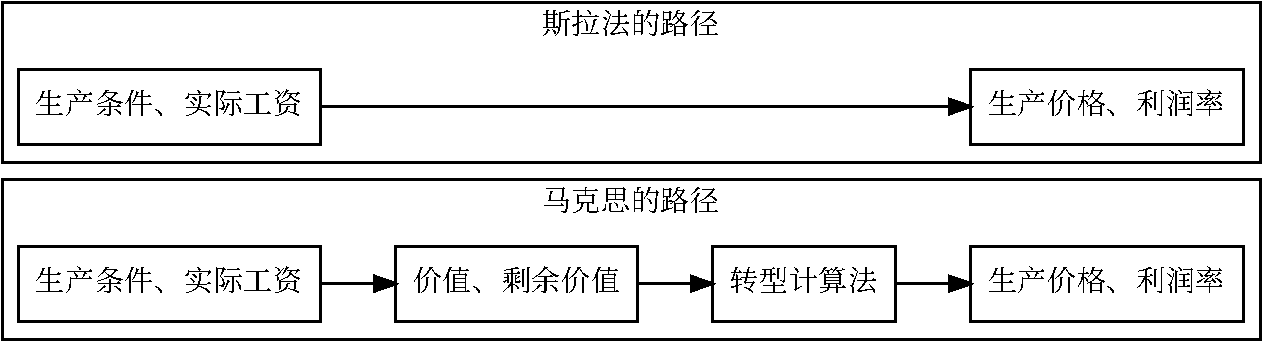
\includegraphics[width=0.8\linewidth]{data/marx1929-1990/sraffa1} 
\label{fig:sraffa1}
\end{figure}

斯拉法对转型问题的“解答”,\textbf{回避了转型问题,倾向于用生产条件和收入分配的
  数据得出商品价格和利润率这一更为基本的问题来完成。}就数量价值论而言,马克思的方
法\textbf{既过分详细,又掩饰了因果关系的真正实质。}因此,米尔福特、德米特里夫、博
特凯维兹、柴田敬和萨缪尔逊,在对马克思的价值具有逻辑上的优先权的主张提出质疑时,
都在《用商品生产商品》中获得支持他们观点的强有力的根据。

斯拉法的分析同时也强化了一些早期评论家的论据,这些早期评论家曾发现马克思劳动价值
和生产价格的关系方面的其他主张也是有争议的。因此,在\textbf{奢侈品的生产与利润率
  的决定毫不相关}方面,博特凯维兹对李嘉图的捍卫和对马克思的批判是正确的。斯拉法同
时也证实了博特凯维兹的论据,即\textbf{一般而言,利润率不能由马克思的公
  式$\sfrac{s}{c+v}$来表示;证实了肯尼思·梅提出的把价值总计为$c,v和s$是不合适的
  观点;证实了杜冈—巴拉诺夫斯基对马克思利润率下降规律的批判;}还证实了勒尔如下的
谴责,即一旦允许有\textbf{两种生产过程}存在的话,从逻辑上看,是\textbf{劳动价值依
  赖于价格},而不是相反。尽管所有这些批判都很有力量,但斯拉法的分析远远超过了其他
评论家的著作所作出的严格确证。他自己的分析框架,可以用来揭示马克思价值理论中更为
基本的缺陷。\textbf{转型不仅仅是一个“复杂的迂回”,绕远路实际上被证明是不可能
  的。}而且,\textbf{即使}当马克思的扩展的路径是可行的,马克思所认为的能够由此揭
示出的\textbf{重要剥削关系并非总是能够建立起来}。也就是说,“复杂的迂回”被证明是
一个死结。这两个问题构成以下两节的主题,第4节论证了《用商品生产商品》是如何提出使
损失达到最小化的建议的。

\section{“复杂的迂回”不存在}

马克思以及后来的马克思主义经济学的评论家和捍卫者,总是把生产出来的商品的劳动价值
看作是正值。后来,\textbf{伊恩·斯蒂德曼在1975年指出,斯拉法的分析揭示了相反情况的
  存在。}这一结果是很富有戏剧性的。首先,劳动价值可能无法确定或者可能等于零,从而
马克思的转型无法进行,他的通向生产价格的路径根本不存在,只有\textbf{斯拉法的“路
  径”是唯一可行的。}其次,\textbf{劳动价值可能为负,这一点与劳动价值可能是零一起,
  反过来破坏了马克思的基本原理,}即正的利润意味着、并且被决定于正的剩余价值。然而,
实际上,一个正的利润率可以与一个负的或零剥削率联系在一起,同时,正的利润可以与负
的或零剩余价值同时并存。


\begin{table}[H]
\centering
\caption{表\ref{t:Sraffa1}中所表明的体系类型的一个数字例证}
\label{t:Sraffa4}
\begin{tabular}{@{}ccccccc@{}}
\toprule
    & \multicolumn{3}{c}{投入} &   & \multicolumn{2}{c}{产出} \\ \cmidrule(lr){2-4} \cmidrule(l){6-7} 
    & 商品1    & 商品2    & 劳动   &   & 商品1        & 商品2       \\ \midrule
过程1 & 4      & 0      & 1    & \to & 5          & 1         \\
过程2 & 0      & 6      & 1    & \to & 2          & 8         \\ \bottomrule
\end{tabular}
\end{table}

\begin{table}[H]
\centering
\caption{用价格表示的表\ref{t:Sraffa4}体系}
\label{t:Sraffa5}
\begin{tabular}{@{}l@{}}
 $\displaystyle 4p_1(1 + r) + w = 5p_1 + p_2 $\\
 $\displaystyle 6p_2(1 + r) + w = 2p_1 + 8p_2 $
\end{tabular}
\end{table}


\begin{table}[H]
\centering
\caption{用价值表示的表\ref{t:Sraffa4}体系}
\label{t:Sraffa6}
\begin{tabular}{@{}l@{}}
 $\displaystyle 4 \lambda_ 1+1=5 \lambda _1+ \lambda _2 $\\
 $\displaystyle 6 \lambda _2+1=2 \lambda _1+8 \lambda _2$
\end{tabular}
\end{table}

这些结论与直觉是相悖的。\textbf{如果所有的生产过程都使用直接劳动的话,那么产出怎
  么能不具有经过很好确定的劳动价值,而这些价值又怎么能不是正数而是其他的情况?}这
一节探讨第一个问题,下一节探讨第二个问题。我们通过提供两个分别产生不确定的劳动价
值和零劳动价值的数字例证来开始我们的分析。表\ref{t:Sraffa4}描绘了
表\ref{t:Sraffa1}所表明的斯拉法体系中的一种特殊情况。相应的价格方程列在
表\ref{t:Sraffa5}中,其中存在着一个有经济意义的均衡。假设把商品1作为价格衡量单
位(由此$p_1=1$),\textbf{假设延期支付的实际工资是一单位的商品2},那么,如
果$p_1=1,p_2=4,w=4和r=0.25$,就使均衡得以形成。然而,运用马克思的向劳动价值“迂
回”的方法,我们是无法得到这一结论的。表\ref{t:Sraffa6}是用价值表示上述体系,它导
致了不一致的方程的形成:
\begin{align*}
 \lambda _1 + \lambda _2 &=1 \\
  2\lambda _1+ 2 \lambda _2 &=1
\end{align*}

因此,劳动价值无法被计算,结果也就没有明确的价值量可以转化为生产价格。

如果某些劳动价值为零,也会得出类似的结论。这种可能性,在
表\ref{t:Sraffa7}—\ref{t:Sraffa9}中显示出来。如果再把商品1作为价格衡量的单位,假
设延期支付的实际工资是一个单位的商品2,如
果$p_1=1,p_2=\sfrac{2}{3},w=\sfrac{2}{3}和r=0.25$的话,一个有经济意义的均衡是存
在的。但是,与第一个例子一样,马克思的“复杂的迂回”是不可能的。
表\ref{t:Sraffa9}中的价值体系表明, $\lambda _1=0和 \lambda _2=1$,因此商品1的劳
动价值就消失了,同样也就没有什么可转化的了。

\begin{table}[htbp]
\centering
\caption{表\ref{t:Sraffa1}中所表明体系类型的第二个数字例证}
\label{t:Sraffa7}
\begin{tabular}{@{}ccccccc@{}}
  \toprule
  & \multicolumn{3}{c}{投入} &   & \multicolumn{2}{c}{产出} \\ \cmidrule(lr){2-4} \cmidrule(l){6-7} 
  & 商品1    & 商品2    & 劳动   &   & 商品1        & 商品2       \\ \midrule
  过程1 & 4      & 0      & 1    & \to & 5          & 1        \\
  过程2 & 0      & 12     & 1    & \to & 2          & 13        \\ \bottomrule
\end{tabular}
\end{table}

\begin{table}[htbp]
\centering
\caption{用价格表示的表\ref{t:Sraffa7}体系}
\label{t:Sraffa8}
\begin{tabular}{@{}l@{}}
 $\displaystyle 4p_1(1 + r) + w = 5p_1 + p_2 $\\
 $\displaystyle 12p_2(1 + r) + w = 2p_1 + 13p_2 $
\end{tabular}
\end{table}

\begin{table}[htbp]
\centering
\caption{用价值表示的表\ref{t:Sraffa7}体系}
\label{t:Sraffa9}
\begin{tabular}{@{}l@{}}
 $\displaystyle 4 \lambda_ 1+1=5 \lambda _1+ \lambda _2 $\\
 $\displaystyle 12 \lambda _1+1=2 \lambda _1+ 13 \lambda _2$
\end{tabular}
\end{table}

这些结论看起来非常奇怪,因为这里存在着一种\textbf{在单一产品生产过程的脉胳中考察
  劳动价值的倾向,而在这种生产过程中,不确定的劳动价值和零劳动价值是不会出现的,}这
两种情况只会出现于联合生产体系中。但是却不能将其斥为有限关联的复杂细节而不予考虑,
因为它们在任何实际的经济中都是很普通的:例如,对羊的宰杀可以产出羊毛皮、兽皮、血、
内脏和一块块的肉。为这些显然很反常的结论提供一个直观的解释同样也是可能的,如果生
产过程中使用的直接劳动量是正的,那么净产出的劳动价值必须等于这一直接劳动的总量。
表\ref{t:Sraffa4}体系中净产出是$(5-4)+(2-0)=3$个单位的商品1,再加上$(1-0)+
(8-6)=3$个单位的商品2。由于直接劳动投入是$2$,\textbf{这一净产出就必须有$2$个单位
  的总劳动价值。然而,由于每一生产过程是以相同的比例生产净产出,因此在剩余产品的
  组成部分之间分配这一劳动价值是不可能的。}

因此,\textbf{计算单个劳动价值的一个必要条件是,生产过程以不同的比例生产净产出。}在
表\ref{t:Sraffa7}中,可以看到这样的情况。在表\ref{t:Sraffa7}中,净产出
是$(5-4)+(2-0)=3$个单位的商品1和$(1-0)+(13-12)=2$个单位的商品2。但是在这种情况
下,\textbf{就商品1而言,过程2确实具有更高的生产力,而在商品2的生产上,过程1和过
  程2具有相同的生产力。}即使作为一个整体的净产出将会有等于2的劳动价值(等于该体系
中所使用的直接劳动量),\textbf{商品1的劳动价值也必须等于零}。如果我们要让总的劳动
投入不变,而把它的一部分从过程1转移到过程2,那么我们就会在商品2的生产保持不变的同
时增加商品1的生产。由于总净产出的劳动价值必须保持2不变,那么商品1的劳动价值必须是
零。

\section{马克思“迂回”的死胡同}

这一节阐述联合生产的另一个结果,该结果同样对马克思的价值理论造成了损害。即使劳动
价值是确定的和非零的,但有一些可能是\textbf{负数}。正如在
表\ref{t:Sraffa10}—\ref{t:Sraffa12}中提出的第三个数字例证所表明的那样,这一观点会
损害把剩余价值与利润联系起来的马克思的基本原理。和以前一样,假设$p_1=1$,延期支付
的实际工资等于一个单位的商品2,从表\ref{t:Sraffa11}中得出的价格均衡
是:$p_1=1,p_2=2,w=2和r=0.25$。然而,商品2的劳动价值是\textbf{负数},因为从
表\ref{t:Sraffa12}中得出$\lambda _1= 1\sfrac{1}{2}, \lambda _2=-\sfrac{1}{2}$。

\begin{table}[!htbp]
\centering
\caption{表\ref{t:Sraffa1}中所表明体系类型的第三个数字例证}
\label{t:Sraffa10}
\begin{tabular}{@{}ccccccc@{}}
  \toprule
  & \multicolumn{3}{c}{投入} &   & \multicolumn{2}{c}{产出} \\ \cmidrule(lr){2-4} \cmidrule(l){6-7} 
  & 商品1    & 商品2    & 劳动   &   & 商品1        & 商品2       \\ \midrule
  过程1 & 4      & 0      & 1    & \to & 5          & 1        \\
  过程2 & 0      & 16     & 1    & \to & 2          & 20        \\ \bottomrule
\end{tabular}
\end{table}


\begin{table}[!htbp]
\centering
\caption{用价格表示的表\ref{t:Sraffa10}体系}
\label{t:Sraffa11}
\begin{tabular}{@{}l@{}}
 $\displaystyle 4p_1(1 + r) + w = 5p_1 + p_2 $\\
 $\displaystyle 16p_2(1 + r) + w = 2p_1 + 20p_2 $
\end{tabular}
\end{table}


\begin{table}[!htbp]
\centering
\caption{用价值表示的表\ref{t:Sraffa10}体系}
\label{t:Sraffa12}
\begin{tabular}{@{}l@{}}
 $\displaystyle 4 \lambda_ 1+1=5 \lambda _1+ \lambda _2 $\\
 $\displaystyle 16 \lambda _2+1=2 \lambda _1+ 20 \lambda _2$
\end{tabular}
\end{table}

同样,这一结果看起来也很怪,但是却能容易地对之进行直观的解释。表\ref{t:Sraffa10}
体系中的净产出等于$(5-4)+(2-0) =3$个单位的商品1,加上$(1-0)+(20-16)=5$个单位的商
品2,同时\textbf{过程2对两种商品来说都确实具有更高的生产力。结果是劳动会从过程1转
  移到过程2,两种商品作为净产出就会被更多地生产出来。}然而这一更大的净产出所包含
的劳动必须同通过减少生产力较低的过程的操作而节省下来的劳动相等。而这一点只有在一
种商品的劳动价值是\textbf{负数时才是可能的}。

把前一节中的两个数字例证和刚刚讨论的这一例证综合起来,可以推导出一个\textbf{一般
  的结论:只有当净产出是由不同的生产过程按照不同的比例生产出来的时候,而且是当没
  有一个生产过程会在生产力方面起支配作用的时候,所有商品的劳动价值才是可以确定的
  和为正数。}正如我们已经看到的,\textbf{这些条件并不是价格均衡要求普遍存在
  的。}因此,生产过程以相同的比例生产净产出的模型,和一个生产过程比其他生产过程效
率更高的体系,都是完全可以接受的。特别是,一个生产过程在生产力方面占支配地位并不
意味着资本家运用的其他过程是无利可图的。\textbf{在均衡状态中,所有的过程都同样是
  有利可图的。}

就转型而言,\textbf{负的劳动价值}——不同于不确定的劳动价值和零劳动价值——\textbf{不
  需要提出特殊的困难。}用来衡量商品的单位是任意的。\textbf{因此,只要劳动价值是可
  以计算的而且是非零的,用劳动价值作为衡量单位就是可能的。}那么,价格就变成了“每
一单位劳动价值”的价格,或价格—价值比率。如果工资和一个指定的衡量价格—价值比率的
单位已知的话,那就存在一个价格和利润率的解。在劳动价值是负数的情况下,就会出现负
的投入和产出项。\textbf{然而,这仅仅表明,一个有经济意义的解答会包括非正的相应价
  格一价值比率,以致于购买和销售这些商品会包括正的支出。}

但是,现在转型还无法实现马克思所考虑的\textbf{本质问题,即要表明正的利润率源于正
  的剩余价值率。}通过计算不变资本、可变资本和剩余价值的大小,我们发现,在
表\ref{t:Sraffa10}体系中,$c_1= 6,c_2= -8,v_1= - \sfrac{1}{2},v_2= -
\sfrac{1}{2},s_1= 1 \sfrac{1}{2},s_2=1 \sfrac{1}{2}$,因此剥削率是负的,而利润
率是正的($r=0.25$)。对表\ref{t:Sraffa7}体系中的例子进行计算,可以得
出$c_1=0,c_2=12,v_1=1,v_2=1,s_1=0,s_2=0$,该体系中没有剩余价值,即使利润率同
样是正的($0.25$),剩余价值率却为零。


\begin{table}[htbp]
\centering
\caption{斯蒂德曼的例证}
\label{t:Sraffa13}
\begin{tabular}{@{}ccccccc@{}}
  \toprule
  & \multicolumn{3}{c}{投入} &   & \multicolumn{2}{c}{产出} \\ \cmidrule(lr){2-4} \cmidrule(l){6-7} 
  & 商品1    & 商品2    & 劳动   &   & 商品1        & 商品2       \\ \midrule
  过程1 & 25      & 0      & 5    & \to & 30          & 5        \\
  过程2 & 0      & 10     & 1    & \to & 3          & 12        \\ \bottomrule
\end{tabular}
\end{table}

我们也有可能会发现,拥有负的剩余价值和正的利润的生产体系(不是仅仅指一个负的剩余价
值率与一个正的利润率并存)。斯蒂德曼的最初的例子再现于表\ref{t:Sraffa13}中。假设工
资是价格衡量的单位(即$w=1$),延期支付的实际工资包括$\sfrac{1}{2}$个单位的商
品1和$\sfrac{5}{6}$个单位的商品2,那么均衡的条件
是:$p_1=\sfrac{1}{3},p2=1,w=1,r=0.2$。利润总额是$9\sfrac{1}{6}$,是正数,而剩
余价值总额则等于$-1$,是负数。

因此,马克思的基本原理无法在一般意义上成立。\textbf{正的剩余价值率不是正的利润率
  的必要条件,同时正的剩余价值对正的利润来说不是必要的。}所以,一般而言,受剥削的
劳动并不是一个“\textbf{优先的具体的量}……而它有可能被看作是形成利润的最根本的源
泉。”这一点除了价值和剥削理论以外还有其他分支。劳动价值可以是不确定的、负的或为
零这一事实,使得马克思对“运动规律”的最初分析令人怀疑,因为这些规律是用总价值范
畴($c、v和s$)来表示的,而这些范畴则被假定为是已得到明确确定的正数。因此,即使不考
虑其他情况,有些总价值范畴不确定或有反常表示这种可能性,会使得人们对马克思的宏观
经济“运动规律”产生怀疑。

一个特殊的“运动规律”是认为\textbf{资本有机构成随着资本主义发展而不断提高}。针对
这一“规律”,欧内斯特·曼德尔指出:
\begin{quotation}
  资本主义生产方式内部的绝对的限制……在于这样的事实,即在机械化的最后阶段——自动
  化阶段,由于把活劳动从生产过程中排挤出去,结果剩余价值量本身必然减少。资本主义
  与完全自动化的生产是不相容的……因为它不再允许剩余价值的产生。
\end{quotation}

如果把上述观点理解为\textbf{正的剩余劳动是正的利润的必要条件的阐释的话,}那么它早
在1898年就遭到了德米特里夫的\textbf{批判},之后又遭到了斯拉法《用商品生产商品》
的\textbf{批判}。如果假设表\ref{t:Sraffa10}的数字例证中的生产过程是完全自动化的生
产过程的话,那么在每一种情况下直接劳动投入都是零,而不是一个单位。在
表\ref{t:Sraffa11}中,除了$w$项由于不再使用直接劳动而消失外,会和以前正好一样。然
而,一个正的利润率和正的均衡价格依然会存在;假设商品1是衡量单位,答案
是$p1=1,p2=0.7,和r=0.425$,\textbf{曼德尔的论据显然是错误的,它仅仅假设存在一个
  商品实物上的剩余——不管它是否是由直接劳动生产出来的——利润是正数。}

然而,该结论并没有破坏马克思关于资本主义社会所特有的剩余价值理论。根据定义,一个
完全自动化的经济是非资本主义经济,因为它不使用雇佣劳动。然而,\textbf{它确实表明
  了马克思的价值和剥削理论存在一个更加严重的问题。}即使是在不存在计算劳动价值和实
施转型的困难的非自动化经济中,马克思关于劳动力具有创造剩余价值的特性的观点也是成
问题的。例如,在这样的情况下,人们可以计算出石油系数来表明体现于每种商品中的石油
数量,而且也可以运用马克思主义经济学家传统上用于转化劳动价值的相同方法,把这些系
数“转化”为生产价格。而且“当且仅当生产出来的每一商品具有剥削的性质,利润才是正
数…… 生产中使用的每种过去生产的商品都必须能够让出这样一种剩余……以得到某
些……唾手可得的……利润。”\textbf{从这种观点来看,劳动力并没有什么特别之处},这
与马克思的观点相反。

\section{体现马克思精神实质的一个新的斯拉法迂回}

那么,从这一残骸中还能救出点什么吗?必须等到在第14章对转型问题的后斯拉法争论进行讨
论和在第15章对斯拉法本人的著作进行批判性评估之后,才能对这一问题做出全面的回答。
但在此可以概括一下《用商品生产商品》所提出的一种辩护。这一\textbf{辩护仅仅适用于
  剥削理论,而对于修补马克思主义价值理论所遭受的创伤并没有提供任何帮助。}它也没有
提到第4节结尾处明显地提出的问题。然而,由于马克思主义者可能认为价值理论是剩余价值
分析的一个主要工具,他们或许会接受第2节、第3节和第4节的批判,但仍旧认为此处所做的
分析最终会证明马克思政治经济学的核心是有根据的,因为价值理论本身是次重要的,全面
的自动化不会存在,剥削只有在与劳动力联系起来时才有意义(参见以下第14章)。而且,将
要讨论的斯拉法的观点显然是处于马克思主义的传统之中的;它涉及到了马克思的最初争论
中的一个论点,对它进行了严格详尽的研究,然后指出,如果不是从形式上来看,马克思的
这一最初阐述在内容上是正确的。

作为转型分析的一部分,马克思坚持认为:(i)一个生产过程,如果其资本有机构成与整体经
济的有机构成相等,那么该过程生产出来的商品的生产价格就将等于它的劳动价值;(ii)该
生产过程的自身条件足以确定利润率。如果把他的利润率概念和转型的方法看作是没有问题
的,那么这一命题就是正确的。通过把更通用的公式$\sfrac{s}{c+v}$的分子分母都除
以$v$就可以把马克思的利润率公式记作$\sfrac{e}{k+1}$,其中$e$表示剩余价值率,$k$表
示整个经济的资本有机构成。由于$e$在所有的部门中都是相同的,“一般”部门的资本有机
构成等于$k$,该部门的利润率(用它自己的劳动价值范畴,$c、v和s$来计算)必须等于整体
经济中普遍通行的利润率。这意味着,该部门获得的利润是它自己生产的全部剩余价值,而
且仅仅是它自己的剩余价值,因此在马克思的转型过程中,其生产价格等于它的劳动价值。

实际上,这种观点是错误的,这既是由于\textbf{马克思错误地相信利润率可以
  用$\sfrac{s}{c+v}=\sfrac{e}{k+1}$来表示,而且还由于他的转型仅仅适用于产出。然
  而,}斯拉法的分析表明,作为整体经济代用品的“一般部门”的观点,可以给出另外一种
解释,而马克思的观点也可以得到证实。在《用商品生产商品》中,斯拉法认
为,\textbf{通过对不同部门的扩张或缩减,他所考虑的任何一个生产体系的比例都可以被
  改变,而原有体系的特性保持不变。}在这一被斯拉法称之为\textbf{标准体系}的重新安
排的体系中,以下命题成立:
\begin{enumerate}
\item 每一商品的总产出,与该商品作为投入的总计使用量有着相同的比例。
\item 标准体系中的净产出与资本的比率,给出了\textbf{最大利润率},该最大化的利润率
  同样适用于该体系和拥有原有比例的体系。
\item 当把这一净产品(指的是斯拉法的标准商品)作为价格衡量单位时,标准体系中对应于
  任一工资的利润率等于原有体系中相同工资的利润率。
\item 标准商品的均衡价格将等于它的劳动价值,原有体系中的利润率,在标准体系中可以
  表示为剩余价值与资本的比率。借助于一个简单的数字例证就可以说明这些命题。
\end{enumerate}

\textbf{不进入到由联合生产引起的复杂情况中去}这么做是再容易不过了(下面第十五章将
要分析这一问题)。因此,不是使用已经提出过的例证中的一个例证,而是在
表\ref{t:Sraffa14}和\ref{t:Sraffa15}中提供一个新例子。在原有体系中,总的投入一产
出比例是不同的;商品1的比例是一个单位,它与商品2的比例是($\sfrac{45}{28.5})或者
是1.6$,与商品3的比例是($\sfrac{48}{41}$)或者是$1.2$。通过把过
程1扩大$\sfrac{4}{3}$,把过程2缩减到原有规模的$\sfrac{4}{5}$,让过程3维持原有状态
的方式,就可以把这些比例带入到标准比例中去。现在,总的投入—产出比例是相同的:$24
/ 20=36 /30=48 /40= 1.2$。

\begin{table}[htbp]
\centering
\caption{表\ref{t:Sraffa15}中的标准体系赖以建立的原有体系}
\label{t:Sraffa14}
\begin{tabular}{@{}ccccccccc@{}}
  \toprule
  & \multicolumn{4}{c}{投入} &   & \multicolumn{2}{c}{产出} \\ \cmidrule(lr){2-5} \cmidrule(l){7-9} 
  & 商品1    & 商品2  &商品3  & 劳动   &   & 商品1    & 商品2    &商品3   \\ \midrule
  过程1 & 9 & 12 & 6 & \sfrac{3}{16} & \to & 18   & 0 & 0      \\
  过程2 & 5 & 12.5 & 15 & \sfrac{5}{16} & \to & 0 & 45 & 0      \\
  过程3 & 4  & 4  & 20  & \sfrac{8}{16} & \to & 0 & 0   & 48 \\ 
  总\quad 计 & 18 & 28.5  & 41 & 1 & \to & 18 & 45   & 48 \\ \bottomrule
\end{tabular}
\end{table}


\begin{table}[htbp]
\centering
\caption{表\ref{t:Sraffa14}体系的标准体系}
\label{t:Sraffa15}
\begin{tabular}{@{}ccccccccc@{}}
  \toprule
  & \multicolumn{4}{c}{投入} &   & \multicolumn{2}{c}{产出} \\ \cmidrule(lr){2-5} \cmidrule(l){7-9} 
  & 商品1    & 商品2  &商品3  & 劳动   &   & 商品1    & 商品2    &商品3   \\ \midrule
  过程1 & 12 & 16 & 8 & \sfrac{4}{16} & \to & 24   & 0 & 0      \\
  过程2 & 4 & 10 & 12 & \sfrac{4}{16} & \to & 0 & 36 & 0      \\
  过程3 & 4  & 4  & 20  & \sfrac{8}{16} & \to & 0 & 0   & 48        \\ 
  总\quad 计 & 20 & 30  & 40 & 1 & \to & 24 & 36   & 48 \\ \bottomrule
\end{tabular}
\end{table}

斯拉法用符号($1+R$)表示的这个量,既为标准体系也为原有体系界定了最大化的利润率,就
标准体系而言,不管相对价格会发生什么变化,$R$不可能再提高了。就原有体系而言,如果
我们用表\ref{t:Sraffa2}中的价格术语来表示表\ref{t:Sraffa14}体系,并且让工资等于
零(这样,所有的净产出与利润一起增长),结果,利润率就等于$R(=0.2)$,这同样也是最大
化的利润率。更一般地来看,正如斯拉法所指出的那样,原有体系“包括着与标准体系相同
的基本方程,只是比例不同。”而且“特殊的比例无法改变……数学上的特性。”如果把标
准商品作为价格衡量单位,由此在我们的例证中$4p_1+6p_2+8p_3=1$,工资被设定在任一可
行的水平上的话,那么,由于这一特性,利润率在标准体系和原有体系中将会是相同的,用
标准体系中的范畴术语可以得出一个更简单的表述:
\begin{equation}
r=\frac{净产品—工资}{用价格表示的生产资料总量}
\end{equation}

如果斯拉法假定整个体系中使用的总劳动等于一个单位,那么
\begin{equation}
r=R(1-w)
\end{equation}
其中$w$是工资(用标准商品单位来衡量)。因此,就我们的数字例证而言,在原有体系和标准
体系两种体系中,如果$w =0.5,那么r=0.1$。

反过来,这也承认了马克思主义对利润率的描绘,任一生产体系的净产品的劳动价值必须等
于该体系中使用的直接劳动总量(参见以上第3节)。因此,在标准体系的情况下,直接劳动总
量必须等于一个单位,标准商品的价格等于其劳动价值。而且,标准体系中的利润率总是可
以表示为该体系的剩余价值与生产资料总量的劳动价值的比率。标准体系中净产品的劳动价
值可以分解为$v_s和s_s$,其中$v_s$是工资的劳动价值,$s_s$是余下的剩余价值,下
标$s$表示标准体系。标准体系中生产资料的劳动价值同样可以表示为$c_s$。因此,最大利
润率($R$)等于$\sfrac{v_s+s_s}{c_s}$。我们已知$r=R(1-w),而(1-w)$仅仅是标准体系中
净产品的比例,它趋向于利润,由此:
\begin{equation}
  r=R(1-w)=\frac{v_s+s_s}{c_s} \frac{1-v_s}{v_s+s_s} = \frac{s_s}{c_s}
\end{equation}
这是剩余劳动或者是剩余价值与雇用资本的劳动价值的比率。很显然,如果$c_s$是正数的话,
那么正的$s_s$是正的$r$的充分必要条件。把(13.3)的分子分母分别除以$v_s$得出:
\begin{equation}
r=\frac{s_s/v_s}{c_s/v_s}=\frac{e}{k}
\end{equation}
因此,马克思主义基本原理的这一观点凭借剩余价值率和利润率也得到了维护。\textbf{而
  且,由于对任一工资水平来说,标准体系中的利润率都必然等于原有体系中的利润率,那
  么原有体系中的利润率也可以表示为剩余价值与资本的比率。}

米克总结道:
\begin{quotation}
  斯拉法对其“标准”部门中利润率与生产条件之间的关系所做的精确假定,与马克思对
  其“平均资本有机构成”部门中利润率与生产条件关系所做的假定是相同的——从这一观点
  看,斯拉法的“标准部门”从本质上讲是试图用这样一种方式来界定“平均的生产条
  件”以得出与马克思一直在寻求的结论完全相同的结论。
\end{quotation}

\textbf{从这一角度看,标准体系使得资本主义体系成为透明体,使得“隐藏的东西能够显露出
来”}。当然,这也正是马克思在其所有关于价值和剥削的著作中试图达到的目的。

\section{结论}

从总体上看,斯拉法的《用商品生产商品》与马克思主义政治经济学有着\textbf{模楞两可}的
关系,在这本书中,价值理论被证明只有在\textbf{特殊情况下才是有效的},马克思自己对
其剥削理论的阐述也同样被证明不具有普遍意义。\textbf{联合生产会使这两个理论显得空
  洞,或者会得出反常的结论。}但是斯拉法没有提到质量价值论方面的问题。因此他的处理
方案是不全面的,而他自己设计的标准商品或许会拯救马克思剥削理论中的一种形式(但是,
见下面第十五章)。而且,正如我们将要在第十五章中所看到的,许多斯拉法主义者认为,由
于斯拉法的范例与马克思的范例同样处在经济学的“剩余传统”中,马克思主义经济学实际
上由于斯拉法的著作而得到了加强,因为马克思自己的特定形式的剩余经济学的缺陷被暴露
出来,并且被证明与剩余方法本身是无关的。同时,斯拉法的批判也指出了马克思经济学中
严重的局限性,而这样做就导致了整个剩余传统受到质疑,包括由马克思所发展了的特殊看
法。然而,在我们将要在第十五章讨论这些更宽泛的问题之前,我们必须讨论“斯拉法革
命”对转型问题的处理所造成的影响。



\chapter{斯拉法之后马克思的价值理论}

\section{引言}

正如前一章所指出的,斯拉法《用商品生产商品》的影响并不是直接的,最初的影响是对新
古典主义理论产生冲击,导致了20世纪60年代中期的“\textbf{剑桥之争}”。尽管这与马克
思对“庸俗经济学”的分析息息相关,但是它并没有对马克思政治经济学自身逻辑上的一致
性产生影响。直到20世纪70年代,它对马克思经济学的直接影响才开始被意识到。同时,由
弗朗西斯·塞顿和保罗·萨缪尔逊在20世纪50年代提出的问题也期待着答案(参见以上第12章)。
有待观察的是萨缪尔逊的结论能否推广为 $n$ 部门模型,以及\textbf{(如同恩格斯和其他
  人曾设想过的)价值向生产价格的转化能否被合理地看作是一个逻辑的和历史的过程}(参见
本书第一卷第3章第2节)。另外,没有解决的问题还有与评价马克思价值理论中数学模型的作
用有关的重要方法论问题,以及价值理论问题中质和量方面的相对重要性问题。

本章的大部分、但非全部,采用的是编年体的形式。下一节探讨的是(非常稀疏地)出现
于1958年和1971年间关于转型问题方面的文献,那时萨缪尔逊以其发表在《经济文献杂志》
上的一篇引起激烈争议的长文而再次加入这场争论之中。第3节概括评述了萨缪尔逊同马克思
主义批评家之间爆发的激烈论战,第4节讨论20世纪70年代中期森岛通夫和斯蒂德曼在价值分
析上的贡献的重要意义,这在以上第13章已经作过概述。森岛通夫也卷入了重新展开“历史
上的转型问题”的讨论,对此将在第4节进行评价。

从20世纪70年代末开始,出现了几种解决转型的逻辑问题的新的尝试,加上20世纪80年代间
出现的某些附加的难点,这些内容构成了第6节的主题。第7节不再按年代顺序,而是按主题
安排的,它简要地论及20世纪最后20年间涌现出来的对\textbf{劳动价值论}的一系列异议,
这些异议与转型问题并没有直接的联系。最后第8节包括20世纪90年代初支持马克思价值和剥
削理论的一些结论。然而,要注意的是,从某种程度上讲,第15章可以被理解为是这一章的
扩展性的结论。这里所探讨的一些实质的和方法论上的问题,将在第17章对“理性选择的马
克思主义”评价时再次出现。

\section{早期的贡献}

20世纪60年代,对转型文献的最重要的贡献是罗纳德·米克对斯拉法的评论,该评论在以上
第13章第5节已作了概述。除此之外,在这10年间,发表的有意义的文章甚少。迟至1973年,
莫里斯·多布还抱怨这一讨论“还留有……某种程度的限制,甚至是很深奥的;这一讨论的大
部分内容并没有在马克思的追随者和解释者中引起多大的兴趣(或者是注意),这些人已转而
集中研究危机和帝国主义问题了。

1961年,森岛通夫和塞顿都声称,转型过程可以按照\textbf{相反的方向}进行,也就是
说,\textbf{通过运用与生产条件和净产品分配有关的资料,生产价格可以决定劳动价值。}他
们从这一点得出结论,认为实证主义者对劳动价值论的异议是没有事实根据的。正如琼·罗宾
逊(和其他人)曾经提出的,价值不是一个形而上学的概念。“不管马克思的价值概念作
为‘现实’描述或者行动向导上的有用性或不相关性如何,至少从操作上讲它是有意义的。

两年以后,挪威人\textbf{利夫·约翰森}又回到世纪之交曾引起好几个著述者兴趣的一个主
题,即\textbf{把劳动价值论和边际效用分析调和起来的可能性问题}(参见本书第一卷10.5
价值分配理论)。约翰森设计了两个价格决定模型。\textbf{在第一个模型中,工人}拥有维
持生存所必需的条件,它决定了传统的马克思模型中的\textbf{均衡实际工资},\textbf{而
  资本家则使得预算约束条件下的新古典主义效用函数最大化。这时,边际效用决定的是资
  本家消费的商品的数量,而不是其价格。在第二个模型中,工人和资本家都有效用函数,
  如果没有一个单独的收入分配理论或者——约翰森提出的变形的——反映工人最低效用水平的
  详细说明的话,利润率就无法确定。现在价格间接地受到边际效用的影响,}因为工人效用
函数中的任何变化都会影响到利润率,从而改变生产价格。

塞顿1957年的那篇文章发表之后,一个在价值和剥削问题的分析中更加热衷于运用数学技术
的时代开始了。然而,起初几乎没有人对这两篇文章作出反应,同样地,置盐信雄在1963年
的一篇文章中对转型问题所做的相当关键的评论,也没有引起任何反应,人们仅仅记住了它
对马克思利润率下降原理的攻击(参见第7章第3节)。在由萨缪尔逊挑起的争论开始之前,另
一本重要的著作是安德拉斯·布罗迪的《平衡、价格和计划》,该书先用匈牙利文出
版,1970年又以英文再版。正如我们将在以下第5节和第6节所看到的,布罗迪预测到了后来
争论的若干方面的问题。但是他的著作在西方没有造成多少直接的影响,恐怕在东方造成的
影响会更小,因为在东方,有创造性的知识分子的努力仍旧碰到到巨大的障碍。

在这些年里,米克对斯拉法的解释大部分被忽视了,只有一个有意义的例外:斯拉法在剑桥
的同事\textbf{莫里斯·多布},开始同他本人的许多共产主义同事分离开来,这是由于他坚
持认为,\textbf{《用商品生产商品》对马克思作了证明},这个证明不亚于该书对新古典主
义经济学诅咒似的控告。在1970年发表于荷兰《经济学家》杂志上的一篇非常有影响的文章
中,多布把斯拉法置于\textbf{古典的传统}之中,他认为这一古典的传统包括卡尔·马克思
以及博特凯维兹和德米特里夫(参见本书第一卷第3章第4节和第5节)。这一切都表
明,\textbf{利润率依赖于投入生产部门的生产条件(不管是工资品还是不变资本的组成要
  素),并且只能依赖于这些生产条件。}多布强调,在与马克思不一致的关于分配理论的少
数几篇评论中,斯拉法没有提供什么东西。\textbf{在斯拉法的模型中,资本家对生产资料
  的垄断是固有的,甚至他把工资当作是剩余产品的组成部分的作法,也可以看作是对现代
  资本主义状况的符合实际的反映。。}

多布在其最后一本书中,对这些观点做了进一步阐述,他重点介绍了斯拉法、古典经济学家
和马克思之间在方法论上的相似性。\textbf{所有这些人都认为,从逻辑上
  看,\CJKunderdot{分配独立于交换},在任何情况下,价格都是取决于收入分配(再加上生
  产条件),而不是相反。}这一“前杰文斯决定规则或模式”使他们的观点同新古典主义理
论家的观点非常明显地区别开来。。以下第15章将对这一在经济思想史上非常有影响力的解
释进行评价。

\section{萨缪尔逊争论}

1969年或者是1970年,萨缪尔逊从美国国家科学基金获得津贴,资助他对马克思价值理论的
研究。第二年他发表了他的这一研究成果的初步概要。他的一篇较长的论文于1971年发表在
《经济文献杂志》上。。萨缪尔逊的结论主要还是他在1957年就已得出的那些结论(参见以上
第12章第2节)。劳动价值理论是一个复杂的迂回;生产价格和一般利润率可以直接地取决于
与生产条件和收入分配有关的信息;因此,马克思的剩余价值理论对于理解资本主义经济中
的利润来说是不必要的。

萨缪尔逊早期的文章虽然被马克思主义经济学家所忽视,但1971年发表的这篇文章却引起了
一场激烈的争论。这种批判性反应上的不同,可以举出好几个理由。对马克思主义的一般性
兴趣增强了,而且同以前相比,有更多的马克思主义经济学家以学术研究为专职。《经济文
献杂志》与更加令人生畏的《美国经济评论》相比,其专门性不太强,但却有更多的读者。
到了1971年,萨缪尔逊已成为正统经济学的一个起统率作用的人物,与20世纪50年相比,他
有了一个更高大的公众形象。1970年,他获得了诺贝尔奖,各种介绍他的著作版本,在销售
量上已远远地超过其他以英文出版的经济学著作。全世界的一届届的大学生从萨缪尔逊的
《经济学》中学到了他们最基础的理论。最后,还有一个风格问题。1957年发表的文章在语
气是上有节制的,而且还带着学术的腔调,但是1971年发表的文章的大部分则相反,而且带
有(并且是蓄意的?)挑衅。
\begin{quotation}
  当你穿越代数学的迷宫,开始理解正在发生的事情时,你发现“转型的算法”可以精确地
  表述为下述形式:“\textbf{反复思考两种可以替换但却又不一致的体系,写下一个。现
    在通过用一个橡皮把它擦掉来进行转型,然后再填上另一个。如此你就完成了转型的算
    法。}”运用这一技术,可以进行从燃素到熵、从托勒密到哥白尼、从牛顿到爱因斯坦、
  从《创世纪》到达尔文的转型——然后是从熵到燃素的转型……这种无可争议的无聊真理,
  在目前已持续34个世纪的冗长文献中的任何地方都没有得到强调,这告诉我们需要对转型
  问题进行系统的考察研究。
\end{quotation}

正是这一“\textbf{橡皮原理}”而不是其他东西,激怒了马克思主义读者。当时的《经济文
献杂志》编辑,马克·珀尔曼,很快收到了大量批判性的短文和评论。他的反应相当迟钝。同
意出版的那些仅有的投稿,均来自于杰出的\textbf{学院式经济学家}。在两篇相当筒短的投
稿中,阿巴·勒纳异乎寻常地指责萨缪尔逊“对如此彻头彻尾地遭到破坏的劳动价值论作了无
根据的让步”;而\textbf{琼·罗宾逊则声称萨缪尔逊对古典马克思主义和新古典主义模型进
  行了折衷。威廉·鲍莫尔}则认为,萨缪尔逊误解了马克思的意图,马克思
\begin{quotation}
  主要关注的是\textbf{利润和剩余价值}之间的关系,仅仅偶尔(作为达到前者的工
  具)关注\textbf{价格和价值的关系}……似乎显示出土地是地租的源泉,资本是利润和利
  息的源泉的竞争过程,仅仅是一个\textbf{分配现象},它掩盖了劳动才是产出的唯一有社
  会关联的源泉的事实。这正是马克思的劳动价值论和转型问题分析的重要意义。
\end{quotation}

萨缪尔逊否认这一点,相反强调他的“擦除和取代原理”同样适用于剩余价值向利润的转化。
鲍莫尔反击说他的文章是致力于研究马克思的目标的本质,而不是研究他是成功还是失败这
一不同的问题。最后,森岛通夫对他于1973年正值辩论高峰期出版的著作《马克思的经济学》
进行了捍卫。他相信他对马克思的批评比萨缪尔逊的批评更严厉,然而还是提供了马克思的
基本观点能够得以保留的论据。

这些投稿没有一篇是特别深刻的,但是以后投往《经济文献杂志》的一系列评论却没有发表。
珀尔曼反而任命马丁·布朗芬布伦纳去“对那些未正式介入新近一轮‘马克思主义——现代主
义’论争的经济学家进行概述”。他的概要是否包括六篇被拒绝发表的文章的摘要并不很清
楚,但这正是他所提供的。他指出,他们的腔调从“学术式的到漫骂式的。”从布朗芬布伦
纳的描述来看,似乎只有一篇文章明确采取的是新古典主义观点,有四篇是试图对马克思的
价值理论进行捍卫。很显然,珀尔曼对发表文章的选择并不是不偏不倚的,而且萨缪尔逊在
一部分标题为“引证的著述者的反应”栏目中发现,该栏目“对那些没有被同意发表的夭折
文章所进行的评论有些零散。”

有两篇曾遭到拒绝的文章后来在别处发表了。资深议会共产主义者\textbf{保罗·马蒂克},
提出了三个实质性的观点。第一,\textbf{他(正确地)强调马克思的价值理论与资产阶级均
  衡分析共同具有成为一个“理论装置”或“思想结构”的特性,因此,马克思的价值理论
  不能被直接观察到。}第二,他认为马克思主要关心的问题是“\textbf{为什么社会劳动关
  系是以价值关系表现出来?”马克思曾经提出“价值概念怎样才能全部呈现出来”(首
  先?)。}他发现答案就在资本主义生产方式的特殊阶级关系中。这里暗含着价值理论质的方
面和量的方面之间的一个区别,这一区别既构成萨缪尔逊其他方面批判的主要特色,又被用
来反对马克思的斯拉法主义批判家(参见以下第15章)。第三,马蒂克认为,\textbf{劳动价
  值论只有在整体经济的水平上才能得以证实:“价值规律不是在每天的价格关系中得到证
  明,而是在生产价格的总体升降过程中找到经验证明的……该体系作为一个整体对价值分
  析是敏感的。}”森岛通夫在后来得出了一个更加严格的相关结论(参见以下第4节)。马蒂
克坚持认为,萨缪尔逊对此一无所知,他是一个庸俗经济学家;他的代数学是“夸大的垃
圾”,他“浪费了自己的时间和国家社会基金会的金钱。”

如果马蒂克是把学术腔调和漫骂口气结合在一起的话,那么\textbf{戴维·利伯曼}对萨缪尔
逊的攻击则采取一种严谨的模式。利伯曼首先提出了他自已解决\textbf{转型问题的几何学
  方案},该方案\textbf{取消了传统的不变条件},包括价格总额与价值总额相等和(或)剩
余价值总额与利润总额相等,\textbf{要求剥削率不管是用价值表示还是用价格表示都要相
  同}。利伯曼为这一修正提供的正当理由是:工人与资本家是围绕着剥削率而不是利润率而
展开阶级斗争的。跟马蒂克一样,利伯曼也抱怨萨缪尔逊仅仅探讨了该问题的\textbf{量的
  方面},而忽视了更有意义的\textbf{质的方面}。萨缪尔逊完全无法理解“\textbf{价值
  问题是一个社会范畴}”,因此“在马克思主义意义上说”,他自我暴露为“\textbf{一个
  可怕的政治的经济学家}”。利伯曼总结道:“为了推进争论中他这一方的发展,(萨缪尔
逊)必须跨越‘哲学—社会学’和‘经济分析’之间的随意界限,以面对作为社会关系范畴的
价值的定义”。

\textbf{价值质的问题和量的问题}之间的这一关键性区别首先起源于马克思的分析,斯威齐
在其著作《资本主义发展论》中对此作了强调。\textbf{1975年霍华德和金提出},应该把这
一区别有效地应用于收入分配的分析中,而这一点实际上包含在了鲍莫尔对萨缪尔逊的批判
中。在对利伯曼当时未发表的文章所做的(必要的)简短评论中,萨缪尔逊把整个观点看作是
包括“一个几乎是滑稽可笑的拜物教和双关语”的错误概念而不予考虑。这是完全不正确的。
萨缪尔逊的错误可能在于:\textbf{通过把洗澡水(量的方面)和孩子(质的方面)一起倒掉而
  弱化了他自己分析的影响力。}实际上,对价值的这两方面\textbf{在逻辑上是分离的}问
题可以作出强有力的证明。如果真是这样的话,那么在取消——按照萨缪尔逊的理由——马克思
数量价值理论的同时接受其对质量问题分析的本质是可能的。利伯曼拒绝这一结论,斯威齐
最终对此也是畏缩不前,但是它却吸引了一些不太教条的捍卫者,他们认为质量价值理论与
斯拉法主义者和马克思主义者之间和平共处的明显承诺之间,存在着持续的关联性(参见以下
第15章)。

马蒂克并不是把萨缪尔逊当作是庸俗经济学家的唯一的评论家,他自己坚决否认这一指
责:“在这一讨论中我的优势之处不是新古典的,而是\textbf{斯拉法}的!……我所说的是
非新古典主义者\textbf{琼·罗宾逊}一直在说的”。萨缪尔逊也不否定传统的分配理论,只
是拒绝与之站在一起。他所希望做的就是打破把马克思看作是一个预言家的神话,他揭露
了“藏在事物表面之下的无法服从于传统政治经济学的秘密。”正如我们已经看到的,在这
一方面,他只是部分地成功了,因为他没有认识到价值理论质的方面的重要性。然而,在这
场论战的最后,\textbf{萨缪尔逊}确实从他1971年的攻击中\textbf{退却了一点},减弱了
他对“橡皮原理”的固执,把马克思描述成为“\textbf{一个政治经济学最初的有创造力的
  缔造者}”。

\section{森岛通夫和斯蒂德曼加入论战}

与此同时,在大西洋彼岸也进行着一场激烈的争论。这场争论首先集中在莫里斯·多布对古典
马克思主义综合的认同上(参见以上第2节)。多布是英国马克思主义经济学家的老前辈,是英
国共产党最重要的理论家(尽管偶尔也持异议),也是斯拉法在剑桥的密友,鉴于斯拉法对由
他的著作引起的争论持绝对沉默态度,多布对其观点的解释迅速成为典范的形式,多布本人
也成为正统马克思主义捍卫者攻击的主要对象。

攻击的最初阶段是在新成立的杂志\textbf{《经济与社会》}上展开的,其中首先是杰夫·皮
林接着是苏珊娜·德·布隆豪夫,对李嘉图的价值理论和马克思的价值理论之间的主要区别进
行了鉴别。他们认为,李嘉图的方法与马克思的方法截然不同,这表现在辩证法、矛盾、历
史特殊性,以及形式和内容之间、本质和现象之间、质和量之间的区别等各个方
面。\textbf{马克思的概念是独一无二的;}在古典政治经济学中找不到他对使用价值和交换
价值、抽象劳动和具体劳动的分析的对等物。首要的是,正如马克思已经认识到
的,\textbf{李嘉图由于混淆了价格和价值而受到批判。}因此,多布对价值理论中“古典马
克思主义”传统的发明是相当错误的。

多布的同事\textbf{鲍勃·罗松}在对他称之为\textbf{剑桥学派、英国—意大利学派或“新李
  嘉图”学派}的一个广为人知的\textbf{批判}中,(从一个稍微不同的角度)得出了类似的
结论。(现在更一般的提法是\textbf{“斯拉法”}学派。)罗松特别不赞成把马克思理解
为“仿佛他是一个英国古典经济学家”。\textbf{实际上,马克思早已对李嘉图把剩余价值
  仅仅看作是一个单纯的分配现象的观点进行了攻击,正是这一观点导致李嘉图忽视了生产
  过程。}同时,马克思也批判李嘉图混淆了劳动力和劳动,批判他无法区分\textbf{不变资
  本和可变资本}。罗松强调,由于受到李嘉图分析的影响,新李嘉图主义者无法理解马克思
的生产方式概念,因此夸大了生产的技术方面,而牺牲了它的\textbf{社会方面},把生产看
成是“一个非社会的或自然的过程”。由于新李嘉图主义的代数学与几种不同的生产方式都
一致,因此就无法验证马克思主义\textbf{关键的历史性特征}。真正的危险在于,马克思主
义者会陷入一场\textbf{争论的束缚}中,这场争论所参照的条件一方面由诸如庞巴维克这样
的庸俗经济学家,另一方面由诸如博特凯维兹这样的新李嘉图主义者来规定。。

\textbf{罗纳德·米克}在其著作《劳动价值论研究》第二版(1973年)的长篇的导言中,已对
这些观点所存在的弱点进行了证实,他展示了怎样使斯拉法的高度抽象的再生产模型变得具
有\textbf{历史和社会的具体性}。米克运用马克思的“逻辑—历史的方法”,对一系列斯拉
法模型作了系统阐述,从简单商品生产开始,从不同部门具有不同利润率的早期资本主义阶
段成功地过渡到《资本论》第三卷所描绘的单一利润率普遍通行的成熟资本主义阶段。米克
总结道,\textbf{斯拉法不情愿以这种方式提出他自己观点的做法,并没有使他成为一个庸
  俗经济学家,也没有使分析价值和剥削理论的统一的古典马思主义方法变得无效。}

在这一点上,森岛通夫将其杰出的才华倾注在马克思主义经济学的研究上。除了布罗迪的文
章以外,\textbf{森岛通夫出版于1973年的《马克思的经济学》,是第一部用数学语言分析
  这一主题的长篇著作},接着就是在《计量经济学》上发表的一篇有着同样难度的文章,再
后来是与乔治·凯特福斯合著的关于这些观点的更为流行的一篇文章。森岛通夫似乎成了系统
探索由联合生产、固定资本和存在可替换生产过程所提出的劳动价值论问题涵义的第一人。
正如马克思所理解的,\textbf{在某些情况下劳动价值可能是负的或不确定的}(参见第13章
第4节),更多地受诺伊曼的而不是受斯拉法的影响,森岛通夫认为,\textbf{通过把一个商
  品的价值重新界定为生产它所需要的最小劳动量,这些困难能够被克服,而且也才能被克
  服。}当按照这些\textbf{“真实”或“最优价值”}来计算必要劳动和剩余劳动的时
候——而且\textbf{只有在这个时候}——森岛通夫所说的“马克思主义基本原理”\textbf{才能
  够普遍地成立:一个正的剥削率必须有一个正的利润率,反过来也是这样。}

从马克思主义角度出发,对这一点所持的\textbf{异议是双重的}。很显然,\textbf{这并不
  是马克思用来界定价值的方式}(它也不可能是马克思用来界定价值的方式,因为在马克思
生活的年代,相关的数学方法还没有发明出来。)而且更重要的是,\textbf{森岛通夫的“真
  实价值”是非加总的,这意味着不再有可能把商品界定为体现于商品中的不变资本、可变
  资本和剩余价值之和。}但是,马克思的许多最著名的观点,都是建立在价值确实是加总的
这一假定之上的,而且他还认为这一加总的特点太明显而无需加以证明。例如,一旦加总的
价值被取消的话,《资本论》第二卷的再生产模型就必须重新表述。因此,森岛通夫用冯·诺
伊曼的方式对马克思主义经济学的重新铸造具有远远超过价值和剥削理论的许多分枝。而且,
尽管森岛通夫已经表明在联合生产的条件下,马克思主义基本原理还是有可能得到保留,但
是他没有这样做的欲望,更不用说这样做的必要性了。换句话说,森岛通夫的价值分析自身
也可能仍旧被看作是一个“\textbf{复杂的迂回}”。

\textbf{伊恩·斯蒂德曼}不久就颇具说服力地把这些问题提了出来。斯蒂德曼在1975年发表
在《经济学杂志》上的一篇论文(参见以上第13章)中承认,如果运用森岛通夫
的“\textbf{真实价值}”的话,负的剩余价值与正的利润之间的矛盾就可以避免了。但
是,\textbf{却没有使人非相信不可的理由去这样做。}斯蒂德曼在他的《斯拉法之后的马克
思》一书中认为,“凡是可以用价值量来表示的任一事物,\textbf{不用价值量也可以表示
  出来,因为价值量仅仅是更基本的物质生产条件和实际工资的派生物。}”斯蒂德曼(挑衅
性地)总结道:“可以毫不过分地强调,只有在对后者的信奉是前者发展首要束缚的否定意义
上,为资本主义社会提供一个唯物主义描述的方案才会依赖于马克思的价值分析。”尽管这
一结论来自于一个马克思主义者,他曾在《社会主义经济学家会议公报》和《新左派评论》
上论证过他的观点,但正如几个评论家所提到的,这一结论实际上与萨缪尔逊
的“\textbf{橡皮原理}”是一致的。

那么,\textbf{“斯拉法之后”的马克思还剩下些什么呢?对森岛通夫和凯特福斯来说,}剩
下的就是用森岛通夫的“真实价值”表述的马克思主义基本原理,\textbf{即用剩余劳动解
  释利润。}斯蒂德曼的学生\textbf{杰夫·霍奇森}声称,即使是这一点也是\textbf{多余
  的},因为\textbf{具体劳动概念本身“仅仅是一个隐喻,在任一社会现实和与此相对应的
  现象形式中都缺乏物质基础。”}对\textbf{霍奇森}来说,\textbf{利润的真正基础
  是“用其价格计算”的剩余产品。}在《斯拉法之后的马克思》中,斯蒂德曼认为,斯拉法
的贡献在于为森岛通夫用“真实价值”表述马克思主义基本原理提供了一个基
础。\textbf{但是两年以后,斯蒂德曼追随霍奇森,而不是森岛通夫,否认剩余价值或剩余
  劳动能够解释利润的存在。}它们是“测量剩余[产品]的两种方法…… \textbf{(狭义
  的)剥削的存在和利润的存在仅仅是同一枚硬币的两面,它们仅仅是存在着物质剩余这样一
  个事实的‘劳动’和‘货币’表述。}”

\section{回到“历史上的转型问题”}

几年前,\textbf{安德拉斯·布罗迪}曾针对斯威齐关于“为什么不从价格开始?”的提问,作
出了一个黑格尔式的回答。\textbf{对黑格尔来说,“一种事物的历史就是该事物自身”,
  因此,“我们的观点和范畴是真实过程的反映,按照它们在历史上出现的顺序来展开它们
  是有好处的”。}用马克思的话说,\textbf{由于价值“不仅在理论上而且在历史上优先于
  生产价格”,}因此,如果要切合实际地谈论价格和利润的话,从价值和剩余价值分析开始
是必然的。以后的一些著述者声称,森岛通夫和萨缪尔逊对“历史上的转型问题”的忽视,
反映了他们各自观点中的主要缺陷。

马克思去世后,恩格斯对转型问题的历史方面进行了详细的分析,之后鲁道夫·希法亭又对之
进行了捍卫(参见本书第一卷第3章第2—3节)。在现代的著述者中,\textbf{罗纳德·米克}对
这一问题强调的最多,因为他把这一解答看作是对马克思的\textbf{逻辑—历史方法}的最重
要的证明。米克强调,\textbf{劳动价值论的地位在马克思所概括的每一个不同历史阶段是
  不相同的。}在没有商品生产的社会里,根本不存在交换,因此价值问题就没有被提出来;
或者会发生零星的物物交换,其中的交换比率也是相当偶然的。在这一阶段,价值理论是不
相干的。第二阶段是\textbf{简单商品生产阶段。}在这一阶段,\textbf{劳动价值论无限制
  地适用。在早期资本主义阶段,由于竞争力太弱,无法在所有部门间形成均衡的利润率,
  在这一阶段劳动价值论也是无限制地适用。}然而,到了\textbf{成熟的资本主义阶段,自
  由竞争形成了统一的利润率,正是在这第四阶段,系统地区别于劳动价值的生产价格出现
  了。}最后,\textbf{在后资本主义(社会主义或共产主义)社会,商品生产将被取消,对任
  一价值理论的需求也将随之取消。}按照以上定义,“价值”和“生产价
格”都是\textbf{具体的历史范畴,}而且作为一个历史过程,从前者向后者的转型,产生于
从早期资本主义向成熟资本主义过渡期间。

如以上所证实的,\textbf{森岛通夫和凯特福斯}1975年发表在《经济学杂志》的文章中,对
上述观点提出了\textbf{第一个决定性的挑战}。(70年代中期在这一杂志上允许发表的有关
价值和剥削论文的数量,比在此之前和在此之后发表的数量都多。)森岛通夫和凯特福斯提出
这样一个问题:“什么时代是价值时代?”他们认为,\textbf{简单商品生产不可能是价值时
  代,这既有历史的原因也有逻辑的原因。}从历史上看,即使是在西欧封建社会瓦解的时期,
也从来没有存在过这样一种生产方式。在这一时期,还残存着某些封建经济关系,而当时自
给自足生产的持续重要性和劳动的明显不流动性表明,\textbf{商品生产的发展是不完善
  的。}而且,简单商品生产从逻辑上讲也是不可能的,因为\textbf{抽象劳动这一重要概念
  预先假定要压制对任一劳动的偏好,而没有抽象劳动,价值理论是不适用的。这只有在资
  本主义条件下才会发生。}

那么,“价值时代”是不是对应于米克所说的早期资本主义呢?森岛通夫和凯特福斯也否认
了这一点。他们认为,\textbf{米克的分析忽略了代表着封建主义和工业资本主义之间这一
  阶段的商业资本。商人的利润来自于不等价交换而不是等价交换。很显然,劳动价值论无
  法适用于此。}工业资本的产生包含商人对其活功的扩展,首先是在生产(或家庭)体系中做
承包商,以后是建立工厂。很显然,在这一历史过程中,商品根本不是按照反映其劳动价值
的价格来进行交换。森岛通夫和凯特福斯总结说,\textbf{马克思曾打算把简单商品生产作
  为一个理想的模式或“逻辑表象”,用来说明利润的出现。}这对前资本主义经济中的价格
决定来说没什么意义。\textbf{实际上,商品从来都没有按照它们的劳动价值来出售,转型
  问题应该被看作是一个纯粹的逻辑问题,它的解答从本质上讲成了“一个静止的、永恒的
  分析手段”。}

尽管米克对自己的观点作了捍卫,但是没有什么用处。之后对转型问题的历史地位进行证明
的尝试很少而且是不成功的。\textbf{从转型问题争论方面可以得出三个一般性的结论。第
  一,将“逻辑的—历史的”方法运用于价值理论并不像米克所讲的那么容易;第二,还存在
  这样一种情况,即“我们对在交换和成本与收益的计算还不普遍的社会中的分配和定价了
  解很少”;第三,也是最重要的,借助于价值对价格的历史优先性,是无法挽救(数量)劳
  动价值论的。}

\section{再次提及转型的逻辑}

转型问题具有多面的性质现在是很明显的了。到20世纪70年代末,它已成为各种历史和逻辑
背景下关于价值与价格数量关系的一整套问题。数量理论也充满了对质的思考,在这方面存
在着种种看法和相互的误解。而且,尽管在历史的转型方面,在联合生产、固定资本和可选
择的生产过程的内涵方面,在造成“复杂迂回”的功过(或必然性)方面,还存在着各种各样
的争论;尽管存在着上述所有的情况,讨论的最后结论,还必须提到马克思最初在《资本论》
第三卷介绍的简单的、一种商品、一种生产过程模型中提出的问题。

试图维护马克思的第一个(也是最不成功的)尝试来自于安瓦·赛克,他认为,正如普遍被相信
的,马克思自己的转型过程并没有错,但最好是把它看作是一个重复过程的第一阶段,从这
个过程中最终会产生正确的(博特凯维兹的)生产价格。也就是说,《资本论》第三卷中得出
的价格应该仅仅被看作是一个最初的近似值,应该用相同的算法首先对它们进行计算,然后
再计算“第二阶段”的价格,等等,这样就可以逐渐地达到博特凯维兹的解答。尽管塞克的
观点在当时引起了巨大的轰动,并且至少得到保罗·斯威齐这样的人物的认可,但是他的观点
既不新颖,也不令人信服。在乔治·冯·查洛索夫1914年前的文章中就发现类似观点的萌芽(参
见以上第12章第2节),而当时布罗迪和森岛通夫都曾预先将马尔可夫矩阵应用于转型问题。
正如\textbf{森岛通夫}所提到的,困难在于\textbf{最初的起点是随意的}。霍奇森相当尖
刻地指出,即使不是开始于劳动价值,而是开始于“商品名字在被翻译成塞尔维亚—克罗地亚
语时包含的字母数量”,塞克的复杂过程最终也能够得出一个确切的生产价格的近似值。萨
缪尔逊在瓦西里·里昂惕夫的激励下,也早已设计了一个类似的毫无意义的“莫名其妙”的价
格模型。

更有趣的是亨特和格利克在《新帕尔格雷夫辞典》关于转型问题条目上称作的“\textbf{新
  的解答}”。这一解答首先由法国的G·迪梅尼尔在1980年公开提出,而美国经济学
家\textbf{邓肯·弗利}一直在沿着相同的思路工作,而且他们的观点自此一直得到其他人的
支持。弗利在其《理解资本》一书中作出了最易于理解的描述。假设一个两部门经济,运用
钢和人类劳动生产钢和小麦,在下述条件下:
\begin{align*}
\sfrac{1}{2}钢+ 1劳动 &\to 1钢 \\
\sfrac{1}{4}钢+ 1劳动 &\to 1小麦
\end{align*}
钢和小麦的劳动价值( $\lambda _s$)和( $\lambda _w$)可以用与以前例证中所使用的方式
相同的方式计算出来:
\begin{align*}
\sfrac{1}{2}\lambda _s+1 &= \lambda _s \label{e:after1} \\
\sfrac{1}{4}\lambda _s+1 &= \lambda _w
\end{align*}
得出 $\lambda _s=2和 \lambda _w=1.5$。弗利\textbf{假设货币的价值(在该体系之外产
  生)是一个单位,货币工资是$0.5$。}如果工人仅仅消费小麦,这样他们能够购
买$0.5 \times 1.5=0.33$个单位的小麦。

价值体系现在可以表述如下:
\begin{equation*}
  \begin{array}{*{7}{c}}
  \toprule
  & c & v & s & c+ v+s & e=s/v (\%) & r= s/(c+v) (\%) \\
  \midrule
  钢  & 1 & \sfrac{1}{2} & \sfrac{1}{2} & 2 & 100 & 33\sfrac{1}{3} \\
  小麦  & \sfrac{1}{2} & \sfrac{1}{2} & \sfrac{1}{2} & 1\sfrac{1}{2} & 100 & 50 \\
  总计/平均  & 1\sfrac{1}{2} & 1 & 1 & 3\sfrac{1}{2} & 100 & 40 \\
  \bottomrule
\end{array}
\end{equation*}

(注意,该经济\textbf{不是处于简单再生产的状态下,因为钢的产出量已超过了这两个部门
  所使用的钢的投入量。})要把这些量转化为\textbf{生产价格},弗利提出了\textbf{两个
  重要的假定},这两个假定构成了“新的解答”的\textbf{不变条件}。第一个假定是
让\textbf{价值总额等于价格总额,但这仅仅是针对净产品而言的}(而马克思和博特凯维兹
则坚持这一条件适用于总产品)。第二个假定是\textbf{要求可变资本转型过程中要保持不
  变。}实际上,弗利对劳动力价值进行了\textbf{重新界定}:它\textbf{不再是包含在工
  人所消费的一系列工资品中的劳动,而是货币工资与货币价值\footnote{弗利所说的货币
    价值是在商品生产中耗费的总劳动时间与总增加价值的比率。}的乘积。}那
么,\textbf{价格关系}可以表达如下:
\begin{equation}
  \label{e:after2}
  \begin{aligned}
    (\sfrac{1}{2}p_s + \sfrac{1}{2})(1+r)=p_s \\
    (\sfrac{1}{4}p_s+\sfrac{1}{2})(1+r)=p_w \\
    (p_s-\sfrac{1}{2}p_s) + (p_w- \sfrac{1}{4}p_s)=2
  \end{aligned}
\end{equation}
其中第三个方程使得用价格表示的净产品(左边)和用价值表示的净产品(右边)相
等。\eqref{e:after2}的答案是$p_s=2.208,p_w =1.448和r=37.65\%$,给出如下的价格体
系:
\begin{equation*}
  \begin{array}{*{6}{c}}
  \toprule
  & 不变资本 & 可变资本 & 利润 & 生产价格 & 利润率 (\%)  \\
  \midrule
  钢  & 1.104 & 0.5 & 0.604 & 2.208 & 37.65  \\
  小麦 & 0.552 & 0.5 & 0.396 & 1.448 & 37.65 \\
  总计/平均  & 1.656 & 1 & 1 & 3.656 & 37.65 \\
  \bottomrule
\end{array}
\end{equation*}

“\textbf{新的解答}”的特征是很容易确认的,\textbf{用价值和用价格表示的净产品是一
  样的}($=2$);\textbf{可变资本也是不变的}($=1$)。由此可以得出\textbf{马克思的一
  个不变条件得到满足,因为剩余价值总额等于利润总额}($=1$);整个体系中的剥削率也不
变($=100\%$)。但是钢产品的价值($3.5$)\textbf{低于}其价格($3.656$);用价值表示的不
变资本($=2$)\textbf{低于}用价格表示的不变资本($=2.208$);价值体系中的利润
率($=33.3\%$)低于价格体系中的利润率($=37. 65\%$)。这最后的差异当然曾令马克思非常
焦虑。\textbf{而且转型过程还包含了实际工资的增加},因为工人现在可以购买$0.5
\times 1.448=0.345$个单位的小麦,而不是$0.33$个单位的小麦。\textbf{这意味着价值在
  逻辑上优先于价格的假定已不存在:“分配的假定要求事后的知识,实际的价格体系必须
  在工资率确定之前就是已知的,人们不能一步步地从价值进入到价格。这两个领域必须单
  独加以考虑,而新解答则仅仅提供了从一个领域到另一个领域的详细过程。”}最后,人们
还必须记住,\textbf{这是一个单一产品、单一过程的模型,在这一模型中,还没有遇到由
  联合生产、固定资本和可替换生产方法提出的问题。}总之,“新的解答”在处理转型问题
上与更传统的方法相比是否有了真正的发展还是令人疑虑的;而且两者都没有克服萨缪尔森
提出的运用价值范畴是一个\textbf{复杂的迂回}的指责。

\textbf{所有这一切纯粹是静止的,}也就是说,它所关注的是一个“均衡”利润率和“均
衡”生产价格的特性,\textbf{而不是这些均衡量在竞争资本主义经济中得以建立的过程。马
克思似乎再一次把资本为了寻求更高的利润而在部门间自由转移直到形成一个普遍的一般利
润率看作是不证自明的,尽管他意识到这可能包含着相当多的干扰。}然而,到了20世纪80年
代,事情显然地变得比这更复杂了。

\textbf{伊曼纽尔·法尔约恩和摩舍·马克沃夫}同时提出了这一问题,而H·尼卡多则以非常不
同的方式提出了这一问题。法尔约恩和马克沃夫列举了一系列令人印象深刻的论据支持他们
自己的观点:即\textbf{利润率实际上是极不相等的,即使在部门内部也是如此,而且“等
  价规律”从经验上讲也是错误的。}他们认为,这是\textbf{资本主义竞争过程本身的必然
  结果}:“在对竞争概念某些合理推理的条件下,\textbf{试图推动利润率远离均衡的力量,
  至少与那些推动利润率趋向均衡的力量一样真实、有力。}”这些力量包括技术的不平衡发
展,以及使用掠夺性的低定价战略使竞争者破产的方式,保证长期高额利润。
\begin{quotation}
  要抓住如下的\textbf{基本要点:竞争就其最根本的意义来讲,是一个无序的过程——而且
    竞争越自由,则无序越强烈。因此,竞争更倾向于破坏利润率的一致性而不是保持这一
    一致性,如果这种一致性曾被强加于这一体系的话。}期望通过竞争保持利润率的最初平
  衡,就如希望所有参与比赛的马仅仅由于它们一同起跑而要求它们必须一起到达一样不合
  理。
\end{quotation}

法尔约恩和马克沃夫就此得出结论:必须把\textbf{价格的形成}看成是一个\textbf{随机的
  过程}。唯一有效的价值理论是具有\textbf{或然说性质}的理论,因此马克思《资本论》
第三卷中的具有\textbf{决定论性质}的分析是一个错误。\textbf{不能用均衡价格来衡量经
  济变量},因为这一概念对任何一种实际的资本主义经济来说都是不适用的。\textbf{需要
  有一个非价格的衡量体系,而且——假定劳动的唯一地位是经济活动的“本质”——这只能是
  人类劳动。}马克思在《资本论》第一卷中对于保持劳动价值论的真实性方面应该做得相当
好些。

这是一个引起人们兴趣的观点,\textbf{在马克思把竞争看作是一个动态过程而不是一个静
  止结果的理论论述中,可以为这一观点找到某种基础。}界于个体经济单位的决策和整体体
系的行为之间的\textbf{具有或然说性质的“架桥理论”}的观点是吸引人的。法尔约恩和马
克沃夫\textbf{非常正确地坚持,《资本论》第三卷中平均利润率和相应的生产价格,是在
  资本主义现实中无法直接观测到的理论实体。但是这并不会使这些概念毫无意义,}正如抽
象劳动概念是破坏劳动价值论一致性的一种抽象一样不会毫无意义的。因此,法尔约恩和马
克沃夫的分析是建立在\textbf{超经验主义}的基础之上的,它与任何维护马克思经济方法论
的观点不相一致。

由尼卡多发起的这场争论的参与者,运用与老练的新古典主义理论家处理均衡分析时相类似
的方式提出这一问题。在非常简单的条件下检验各种\textbf{非均衡调节机制},看看该体系
的动力机制能否带来包含平均利润率的生产价格。结果并不令人放心。它们“从对完全不稳
定的论证……到对生产价格至少局部稳定的论证……价格、产出和利润在界限内的波动或摆
动……也可以得到论证。”而且大部分分析“涉及的仅仅是一个流动资本的模型…… 而且这
些已论证的结果依赖于形式化的类型,反映系数和附加的[假定]。”因此,\textbf{收敛问
  题依旧未解决,生产价格和平均利润的理论意义和经验意义也由此成为未解决的问题(}参
见以下第15章和第17章)。

\section{价值理论的其他问题}

关于价值理论的争论并未局限在转型问题上,这一节我们将涉及\textbf{与生产价格起源于
  劳动价值并不直接相关的一些问题。}第一个是集中于\textbf{“劳动力”商品特殊地
  位}的复杂问题。由马克思最初提出的一个难题是\textbf{熟练劳动向非熟练劳动(或复杂
  劳动向简单劳动)“折合”的问题}。一小时的高度熟练劳动要多于一小时的非熟练劳动者
劳动吗?如果是这样的话,那么,如何来计算分配给技能程度不同的劳动者的\textbf{权
  数}呢?马克思本人的答案受到了严厉的批评,既有对其形式上的弱点的批评,也有对其相
对工资论的缺陷的批评。日本马克思主义经济学\textbf{宇野学派}信徒们提出的
是\textbf{另一个激进的平均主义方案,}认为不管从事这一工作的工人的技能或培训的程度
如何,\textbf{一小时劳动就产生一个相同数量的价值。}然而,它没有提供及相对工资理论
或生产价格理论。

另一个单独的问题是关于\textbf{劳动力市场分割问题},它与第一个问题紧密相连而且经常
被混淆在一起。具有同等技能的工人在报酬上的差异是巨大的。这些差异看起来也
是\textbf{系统地而不是随意地依赖于雇主的特性}(例如大公司比小公司付更多的工
资)和\textbf{工人的特性}(少数民族和女工比白人男工获得的报酬少)。对分割的劳动力市
场的早期分析,是由新制度学派经济学家进行的。但是,\textbf{马克思主义者}也普遍地对
这些观点作了证明,他们把这些现象解释为资本在处理其他难以对付的劳动大军中采取
的“\textbf{分割与征服}”的战略。马克思主义者对与之相联系的工资歧视的解释,比其新
古典学派对手的解释更具有说服力,这确实是马克思主义经济学明显地优于传统理论的一个
领域。然而,劳动市场分割必然包括\textbf{无产阶级不同部分之间存在着不同的剥削
  率}。\textbf{这些变化在分析上(和政治上)的充分含义还有待于全面探索。}

近年来,为了排除所有这些困难而被日益频繁地提出的观点是,马克思对劳动力的分析基本
上是\textbf{错误}的。这一观点分为两部分:第一,从定义上看,商品是为了到市场上销售
而生产的,但劳动力却不属于这种情况,因此劳动力不可能是商品。第二,\textbf{表示生
  产条件的系数是由社会因素也是由技术因素决定的};它们是在工作场所就\textbf{劳动强
  度和任务分配}而进行的无休止冲突的结果。这就对劳动力使用价值分析造成了现实的难
题。“对其他任何商品的使用价值的享有是不成问题的:面包无法拒绝被吃掉。
但\textbf{劳动力却不是这样,它的‘使用价值’不是被转移,不是被出售,不是被消费,
  它必须是被榨取”,并且面临着工人在生产过程中有意识的抵抗。马克思的劳动力商品概
  念废除了这一决定性的特性,并(自相矛盾地)威胁到要把阶级斗争从他的政治经济学核心
  中消除。}

这些缺陷与另外一个缺陷紧密相连。女权主义者极其有理地抱怨,马克思的价值理论由于
把\textbf{女性的家庭劳动界定为“有用但非生产性的”劳动而贬低了女性的家庭劳动。}这
一劳动之所以有用,是因为它对于(占优势地)男性劳动力的再生产,从而对资本主义生产方
式自身的再生产来说是至关重要的;这一劳动之所以是非生产性的,是因为它既不生产商品,
也不生产价值,也不生产剩余价值。这并不是马克思试图区分生产性劳动和非生产性劳动所
引起的争论的唯一线索,\textbf{流通费用的增长,国家的大量经济活动(直到最近还呈增长
  趋势)也引起了激烈的争论,}在20世纪70年代这一争论最为激烈。

还必须进一步提及三个难题。\textbf{马克思的地租理论}惯常被他的朋友同样也被他的对手
所忽略,实际上马克思的地租理论在1959年就受到\textbf{萨缪尔逊}的批判,其理由
是\textbf{非生产性使用的投入本身就足以使相对价格同相对劳动价值相背离。}20年后,出
现了一系列的文章\textbf{试图恢复}马克思对绝对地租的分析,该分析与使用自然资源部门
中的价值向生产价格的转型有着密切的关系,马克思的级差地租概念就由此与李嘉图的级差
地租概念区分开来。这个问题的重要意义远远地超出了最初提出的城市土地价格问题,因
为\textbf{只要劳动的使用在一块土地上比在另一块土地上“更具生产性的”意义,就应该
  支付地租。因此,在选择所使用的生产过程时,地租分析和劳动价值定义之间就存在着密
  切的联系。}在把劳动价值论应用到国际贸易方面,特别是用于分析经济发展阶段不同的民
族国家之间或者地域之间的不平等交换时,存在着更进一步的分歧。

最后还有一个\textbf{垄断问题},它在关于转型的文献中几乎是被忽略的。\textbf{假如存
  在着自由竞争和形成一般利润率的强烈趋势,生产价格就是竞争价格}。对垄断问题
的\textbf{一个办法是否认它的存在,}其理由或者是认为\textbf{竞争价格}总是具有强大
的力量,或者认为全球范围内竞争价格由于\textbf{跨国资本}的出现而得到了极大的增
强。\textbf{巴兰和斯威齐采取另一种方法,他们用新古典的均衡垄断价格理论取代马克思
  的生产价格,}这一方法斯威齐已——非常容易引起争论的——把它作为“\textbf{第二种转
  型}”而加以证实。\textbf{第三种分析类型}出人意料地不受马克思主义经济学家欢迎,
它采用的是\textbf{米哈尔·卡莱茨基的寡头定价的“后凯恩斯主义”模型,利润率的等级是
  不同经济部门的资本家享有不同程度的垄断力的表现。}

\section{结论}

战后出现的关于劳动价值论的质的问题的讨论,\textbf{在本质上没有遭受损害。}不管斯拉
法著作的标题怎样,\textbf{生产在本质上仍然是人类活动的过程。交换现象中可以发现社
  会分工。由于生产者通过商品交换媒介而相互联系,他们也由此而相互异化,他们对社会
  现实的直觉被最后出现的商品拜物教所歪曲。}这就是劳动为什么在政治经济学中占据一
个“优越”的位置,以及为什么以上第13章第5节中讨论的“能力”、“谷物”、“花生”价
值理论完全忽略马克思劳动价值论的质的意义的原因。

\textbf{价值论的量的情况则完全不同。}在《资本论》第三卷中,马克思提出了两个大胆的
断言。首先,他认为转型问题是能够被解决的;价格总额\textbf{等于}价值总额,利润总
额\textbf{等于}剩余价值总额,以及在生产价格王国通行的一般利润率是由剩余价值与不变
资本价值加可变资本价值之和的比率事先确定的。\textbf{其次,}他强调价格和利润只能起
源于劳动价值,因此\textbf{劳动价值拥有逻辑上的优先权。}

一般而言,马克思的第一个观点是不正确的。即使是在单一产品、单一生产过程的模型中,
这一观点也只有在非常特殊的假定条件下才有效。\textbf{一旦联合生产、固定资本和可选
  择的生产过程存在的话,这一观点几乎都是错误的。}马克思观点中较不充分的各种看法可
以被证明是\textbf{有根据}的。\textbf{利润率可以表示为生产条件和资本家与工人之间收
  入分配的函数。运用森岛通夫的“真实价值”或冯·诺伊曼的价值理论,利润率可以表示为
  价值量的函数,马克思主义基本原理——正的利润率需要正的剥削率,反过来也是这样——也
  能得到坚持。}只有在这种有所减弱的看法中,马克思的第一个观点才被证明是合理的。

然而,他的第二个观点是错误的,马克思“复杂的迂回”确实是不必要的;正如\textbf{琼·罗
  宾逊}在半个世纪前指出的,\textbf{“马克思用价值概念表示的所有重要的观点,如果不
  用价值概念来表示的话,或许会更好。”特别是劳动价值论对剥削理论来说是不必要的,
  即使是从质的方面考虑也是如此。}正如马克思自己解释的,利润之所以产生,是因为资产
阶级在一个能够产生剩余的经济中垄断了生产资料。阶级垄断是资本家拒绝其他人占有他们
所拥有的生产资料的能力。由于没有生产资料大多数人就无法生存,因此资本家对生产出来
的东西就拥有有效的索取权。按照上面段落中提到的条件,\textbf{利润就可以用剩余劳动
  量来表示。但这仅仅是衡量利润的一种可能的尺度,而且对剥削理论来说它也不是最根本
  的。}

尽管对这些结论仍然存在争论,但是对劳动价值论的量的信奉继续呈下降趋势。那么用什么
理论来取代它呢?许多马克思主义经济学家简单地\textbf{退回到了对价值的质的分析上。
  但随之出现的困难是:}马克思对商品交换、资本积累和危机的分析是运用\textbf{价值术
  语}进行的,这就需要用一个更加容易被接受的方式对之进行重新阐述。许多著述者简单地
采用了\textbf{非马克思主义}的价格理论,\textbf{象巴兰和斯威齐在其著作《垄断资本》
  中所采用的理论(参见以上第6章),霍华德·谢尔曼阐述的准凯恩斯主义的周期增长模型,
  或者是同基斯·考林和马尔科姆·索耶联系在一起的卡莱茨基的垄断资本主义分析。}下一章
我们将评价另一种反应,它更公开地敌视新古典分析,它得自于斯拉法的均衡价格理论,并
试图在此基础上建立一个重新展示马克思对价值的质的分析的根本要素的政治经济学体系,
但没有再使用马克思的价值范畴。

%%% Local Variables:
%%% mode: latex
%%% TeX-master: "../../main"
%%% End:

% \chapter{马克思主义政治经济学和剩余经济学}  

\section{斯拉法马克思主义}

从本质上讲,面对挽救马克思价值论的各种尝试,\textbf{斯拉法经济学家}仍旧保持着镇静,
而且依然继续强调本书以上第13章概括的批判是有效的,即\textbf{重新设计的劳动价值范
  畴,从最好的方面讲是多余的,从最坏的方面讲是引起争议的或错误的。}同时,斯拉法主
义者声称,他们对马克思的分析是建设性的,他们认为斯拉法和马克思同属于一
个“\textbf{剩余范式}”,具有相同的视角和方法论。因此,他们认为他们对马克思的批评
是属于“内部的”批评,马克思主义政治经济学实际上得到了加强,因为其最初形式中的缺
陷被暴露出来而且被证明与支持它的更一般的方法是不相关的。因此,斯拉法的著作提供了
一个牢固的基础,使剩余范式得以发展并使马克思主义的真正洞察力重新得以建立。

这些著述者对剩余所下的定义是不相同的,但\textbf{基本的观点}总是相同的:\textbf{剩
  余形成可处置的资源。任一经济体系的净产出被分成两部分:产品再生产所需要的部分,}它
代表生产或再生产的必要成本,其中\textbf{包括必要的劳动成本};\textbf{净产出的余留
  部分代表剩余。}不管剩余如何使用,这一经济的产出都可以得到保证,虽然剩余的使用会
影响到该体系的动态性(参见以上第6章和第9章)。\textbf{剩余收入没有对应的等价物的交
  换,不代表生产成本。因此,财产收入——通常被认为是剩余在阶级社会里分配的主要形
  式——很容易被认为是剥削的结果},许多斯拉法主义者明确地将其作为一种合适的描述而加
以接受。

在资本主义社会,利润是财产收入的主要形式,\textbf{在竞争中利润的分配通过生产价格
  的形式,生产价格使利润率平均化同时使经济的再生产得以进行。因此,不像新古典主义
  经济学中所说的那样:利润并不表示任一“生产要素”的报酬,价格也不反映相对稀缺
  性。}在这种剩余观点中,存在着一个\textbf{用商品生产商品的“循环过程”,这与新古
  典主义观点中的“从‘生产要素’到‘消费品’的单程路径”相反。}而且在新古典主义理
论中不需要描述\textbf{再生产和剩余}的概念,或者如果附加地提到,再生产和剩余的概念
也没有什么重要的意义;商品可以被生产出来,但没有被看作是再生产的投入和超过生产所
需投入的剩余价值之和。进而对那些坚持剩余范式的人来说,\textbf{正是生产和再生产的
  需要在决定经济行为中起着支配作用,它不能被准确地界定为是自主经济人的选择}(参见
以下第17章)。相反,依据在剩余生产和分配中的作用界定的是\textbf{阶级}。

凭借通常所指的\textbf{作为“长期状态”或“引力中心”的竞争性均衡}这一特殊概念,剩
余理论家们对价值进行了分析。不同部门中的利润率和同类型劳动的工资率分别被设想成是
相同的,同一单位商品以同一价格交易。这些特征在第13章所概括的斯拉法体系中是很明显
的,马克思主义对转型问题的论述很典型地遵循了这一均衡概念(参见本书第一卷第3章和以
上第12章、第14章)。斯拉法主义者声称对这些经济状态的特征曾进行过严格的检验,但马克
思主义者却没有这样做。他们对马克思主义的批判是这一结果,而对新古典主义理论的攻击
则是另一结果(参见以上第13章)。

对这些斯拉法主义者来说,马克思本人价值理论的重要性纯粹是\textbf{历史方面}的:它是
李嘉图经济学衰微之后剩余范式得以保留和扩张的主要媒介。然而,由于诸如德米特里夫、
里昂惕夫和冯·诺伊曼等经济学家后来超越马克思而进一步发展了剩余方法,而且通过这样做
揭露了马克思著作中的重要局限。因此,斯拉法主义者声称,如果马克思主义的真理要保留
的话,成为一个修正主义者是至关重要的。然而,\textbf{剩余范式的现代理论家们,对这
  一范式到底需要什么并未达成一致的观点。}加里格纳尼、伊特韦尔和米尔盖特喜欢直接建
立在《用商品生产商品》基础上的一种方法,而森岛通夫、古德温,可能还有帕西内蒂,特
别是冯·诺伊曼的著作,则认为线性生产理论更有说服力。琼·罗宾逊和后凯恩斯主义者则更
喜欢把卡莱茨基解释的凯恩斯著作作为发展的主要模式(参见以上第5章),而马尔格林和哈里
斯的观点更加具有综合性(参见以下第4节)。所有这些观点的共同特征是:把马克思的观点和
其他经济学家的观点混合起来,特别具有\textbf{冲淡马克思主义成分}的效果,以至于现代
马克思主义政治经济学到底是什么变得模糊不清了。以下事实则进一步加剧了这一倾向,即
对剩余范式特征的界定有时与新古典主义理论相对立,而且对于到底什么才是新古典主义的
本质也存在着不同的看法。

下一节将要概括历史理论家们如何用\textbf{斯拉法的观点来解释经济思想的发展,特别是
  价值理论的发展。}他们强调,自从资本主义出现以后,就存在着两种主要的分析立
场:\textbf{剩余传统和供求理论。}第3节探讨马克思主义者对这一观点的评论,认为把马
克思并入到同时也包括象李嘉图和斯拉法这样的资产阶级思想家的政治经济学的流派中是完
全不合适的。第4节接着对现代剩余理论家们如何试图超越《用商品生产商品》而扩展他们研
究经济学的方法作了概括,第5节则探讨对他们的努力所作的批评。

\section{经济思想史中的剩余传统}

罗纳德·米克和莫里斯·多布很快就察觉到在马克思和斯拉法之间有某些相似之处。他们各自
及时地根据斯拉法的著作重写了经济学史,认为至少从18世纪开始,经济理论就在两种传统
中发展:供求方法和剩余范式。多布坚持认为,亚当·斯密是一个关键性的人物,可以从他的
理论中同时引出这两种传统。李嘉图和马克思在19世纪发展了剩余方法,而德米特里夫、博
特凯维兹、里昂惕夫、冯·诺伊曼和斯拉法则是20世纪发展剩余方法的主要人物。米克的着重
点稍有不同,他对重农主义的广泛了解,导致他抬高了亚当·斯密在现代剩余理论范式的公式
化方面的重要作用;他对历史唯物主义起源的研究加强了这一结论。米克认为,在斯密之前,
没有一个经济学家正确地构思资本主义社会的阶级结构,他们也没有意识到资本主义阶级关
系积累的重要性。此外,尽管米克没有对李嘉图著作在剩余传统中的中心问题提出质疑,但
是他对斯拉法本人对李嘉图经济学发展的解释不应受到指责这一点并不充满信心。在编辑
《大卫·李嘉图著作及通信集》中,多布与斯拉法进行过广泛的合作,因此毫无疑问,多布在
李嘉图理论的确切性质方面受到了斯拉法观点的影响。

米克和多布在运用斯拉法的著作重写经济思想史时,没有遇到什么困难,因为这与他们已有
的观点十分一致。\textbf{1960年之前,他们各自都曾试图把马克思严格地界定在古典政治
  经济学的传统中,认为古典分析不能被简单地看作是新古典主义经济学的萌芽形式(象许多
  非马克思主义的思想史学家所做的那样)。}另外,在斯拉法的批判超出把转型问题看作是
一个“复杂的迂回”的逻辑变得很明显之前,他们都\textbf{已过世}了——多布1976年去世,
米克1978年去世(参见以上第13章)。因此,他们的理论史著促进了那些继续为经济思想史
的“双重传统”解释进行辩解、同时也接受斯拉法对马克思批判的全部力量的更为忠诚的斯
拉法主义者。\textbf{加里格纳尼非常仔细地考察了古典的和马克思主义的价值理论的结构,
  认为这两种理论在逻辑上和历史上都与凯恩斯的有效需求理论相一致。}米尔盖特认为,凯
恩斯可以被看作是一个“长期”理论家,他的分析可以不受20世纪60年代在“资本争论”中
遭到破坏的残余的新古典主义因素的影响。确实,\textbf{米尔盖特和伊特韦尔}曾强调指出,
新古典资本理论的逻辑缺陷完全颠覆了凯恩斯著作的其他解释,而且\textbf{要求把凯恩斯
  理论重新界定在剩余范式之内。}

供求理论的进展也引起了斯拉法主义者的关注。加里格纳尼、伊特韦尔和米尔盖特都曾指
出,\textbf{在20世纪30年代,在希克斯和哈耶克的影响下,新古典主义均衡理论放弃了价
  值理论的传统“目标”——长期均衡。}很显然,瓦尔拉斯关于经济关系的观点从一般意义上
看与一般利润率的存在不相一致。由于这一原因,\textbf{包括资本物品供给价格上的不均
  等收益率在内的内部暂时均衡和短暂均衡的观点,开始代替了长期的重力中心,而这一中
  心以前曾在两种传统中支配着价值理论家的分析。}结合着对新古典主义理论其他形式的致
命批判,\textbf{斯拉法经济学家由此声称,剩余范式是政治经济学唯一连贯的方法。}

多布本人就是这一观点的拥护者。在《用商品生产商品》之前,他就曾用古典政治经济学和
马克思主义政治经济学的优点来攻击新古典主义理论,但他却从来没有对供求分析的逻辑连
贯性展开全力攻击,只是与米克一起声称,它从概念上讲是错误的,从意识形态上讲是有动
机的。在受到斯拉法的影响之后,多布的关注点有了一个重大的转移。多布现在则声称新古
典主义理论的科学地位已完全被削弱;这也就意味着,马克思本人完全击溃庸俗经济学的目
的已达到了。

\section{马克思主义对剩余传统的批判}

\textbf{许多马克思主义者反对把马克思并入到剩余范式中,经常声称斯拉法主义者及其前
  辈本身都是庸俗经济学家。}相反,他们认为马克思主义政治经济学是独一无二的,它
与\textbf{新古典}分析之间有着明显的\textbf{分岐};把马克思主义政治经济学并
入\textbf{斯拉法}的思想源流中,不可能不对马克思主义政治经济学的统一性造成无法弥补
的伤害。这些评论家无需就斯拉法批判马克思价值论的逻辑一致性进行质疑;确实,有些人
承认它在形式上是有一定道理的,但是他们拒绝接受批判马克思时所使用的术语,仅仅接受
了对新古典主义理论的攻击,尽管它也是庸俗经济学(参见以上第14章)。

在为多布的《亚当·斯密以来的价值和分配理论》所写的评论中,\textbf{保罗·斯威齐}提出
了一种温和的批判形式。
\begin{quotation}
  马克思的理论确实是建立在\textbf{李嘉图理论基础之上}的,并且在多个方面\textbf{发
    展}了李嘉图的理论。\textbf{但与李嘉图完全不同,马克思认为他的任务是建立对整个
    资本主义秩序全面的、不妥协的批判,}包括对整个资本主义秩序的运动方式竭尽全力的
  全面的、不妥协的批判。为了完成这一任务,他开辟了一个全新的领域,建立了一
  种\textbf{既反对古典经济学又反对新古典主义经济学的传统…}…在多布看
  来,\textbf{斯拉法就是他所说的传统在当代的化身,}斯拉法著作的书名本身就与马克思
  的方法截然不同。马克思没有着重去考虑“\textbf{用商品生产商品}”,他的主题
  是\textbf{用人类劳动生产商品。}
\end{quotation}
本着同样的精神,其他马克思主义者也曾指责多布和米克两人都贬低了马克思对古典政治经
济学批判的意义。

在这里,有一点是真实的。马克思把一系列的质的特征和量的内容并入到他的价值范畴中。
他阐述了一个“劳动价值理论”和一个“价值劳动理论”。换句话说,\textbf{马克思的概
  念试图用古典政治经济学中所缺乏的一种明确的方式来揭示商品生产体系的社会关系。}我
们可以很公正地指责多布实质上忽略了马克思对古典经济学的批判,指责米克不合逻辑地把
只有在马克思的著作中才清晰地出现的质的特征硬塞进了斯密和李嘉图的著作中。由于这样
做,他们轻视了不连续性,贬低了马克思下述合理的观点,即他的古典主义先辈们的经济学
中渗透着的\textbf{拜物教}观点。马克思的经济学不仅仅是古典政治经济学的线性延续,而
且不论斯拉法对马克思价值理论的量的批评是否有道理,这都是真的。然而,马克思主义评
论家却忽略不谈米克和其他人在质的分析中,试图运用的是同马克思最初建立的框架相并行
的斯拉法框架。更重要的是,他们未能意识到马克思价值范畴的神圣本质使得理论整体结构
的诸方面都存在一种缺陷。\textbf{在经希法亭、比德里和鲁宾到斯威齐和罗斯多尔斯基的
  马克思主义思想史中,发现这样一种只强调价值理论的质的方面、从实质上排斥量的方面
  完全不同的传统,确实是有可能的,}而斯拉法主义者则与作为庸俗经济学的新古典主义理
论家混在了一起。

马克思主义对斯拉法的批判没有提到这一极其基本的要点,但他们提出了两个更为深刻的问
题。第一,斯拉法的批判采用了一种特殊手法,由此决定联合生产方式生产的商品之间具体
劳动的分配,马克思没有发表过这种见解。批评家们认为,这样做的结果就是斯拉法主义者
把太多的意义硬塞到了他们自己的结论中,而最后并没有表明他们对马克思价值的量的分析
的理解是恰当的。第二,\textbf{科学分析仅仅是马克思主义努力成为以转换现存秩序为目
  标的批判性理论的一个基本元素。}在斯拉法的框架中,没有什么东西能够足以弥补由于排
除对\textbf{剩余价值}概念的所有考虑而造成的\textbf{思想政治损失}。

然而,这些论证却无法为“不管怎样继续进行下去”的策略进行辩护,这是某些马克思主义
者面对斯拉法的批判所采取的策略。\textbf{马克思价值理论在量的方面的含糊不清,被反
  对斯拉法的马克思主义者所误用。}第13章中所概括结论中的自负,远甚于在阐述其过程和
假设中的自负。斯蒂德曼的批判家们也总是经常退回到对不确定的和难以理解的价值—价格关
系的“真实”性质的描述中,当然他们也没有对《资本论》第3卷不同于《资本论》第1卷的
价值理论进行演绎的、形式的描绘。\textbf{在《资本论》第3卷中,可以辨认出马克思是处
  在李嘉图传统中},而且这一点也通过恩格斯对“有奖论文比赛”的探讨而得到了进一步证
明(参见本书第一卷第2章和第3章)。而且,劳动价值论的政治—思想作用依赖于它自身的科学
真理。\textbf{科学与政治的分离会威胁到马克思方案的整个基础,正如在斯大林统治下把
  马克思主义用作国家意识形态所展示的那样(}参见以上第2章第3节)。

反斯拉法的马克思主义者从捍卫马克思转到攻击斯拉法经济学的刻板结构时,有着更强有力
的根据。然而即使如此,他们也错误地把斯拉法著作中没有包括的特性硬塞进斯拉法的著作
中。象斯蒂德曼所说的那样,《用商品生产商品》本身没有包括对劳动和循环过程的分析这
一事实并不意味着它无法内在地解决这些问题。指责斯拉法的理论仅仅局限于交换关系,把
生产看作是一个技术问题和并入了拜物教观点等等,是毫无意义的。这一结论是以下述事实
为依据的,即\textbf{斯拉法主义者试图在斯拉法原著的基础上建立一种全面的政治经济
  学,}正如我们将在下一节所展示的那样。

\section{超越价值理论}

剩余理论家们采用了多种多样的研究方案以扩展和丰富他们研究政治经济学的方法。并不是
所有的人都认为《用商品生产商品》是最合适的出发点;有些人更倾向于里昂惕夫和冯·诺伊
曼的模型。但是\textbf{所有的人都认识到,凡是与马克思的观点有联系的地方,必须把这
  些观点并入到非马克思主义理论家的著作中,}包括象凯恩斯和熊彼特这样的反马克思主义
者的著作中。不过,这种修正主义形式不自觉地比许多早期的看法\textbf{更欠积极性},并
且只是把增强马克思主义对资本主义发展的洞察力作为一般目标,而不是对之提出进一步的
质疑。

\textbf{加里格纳尼、伊特韦尔和米尔盖特}不仅强调了斯拉法价值论述的独特优点,而且还
声称该论述准确地反映了作用于资本主义经济的因果关系的总体结构。\textbf{价值理论
  的“目标”——长期均衡,允许把分析集中在通过竞争发挥作用的“持久而系统”的力量上,
  并且把它们从复杂和短暂的失衡影响中抽象出去。}决定均衡价格和其他分配变量的价值理
论的论据(技术、产出和分配的一个变量)反映了在产出、分配、价格和技术进步的实际变化
之间\textbf{缺乏任何一般的因果关系}。其结果是,这些论据中每一决定性要素大部分都相
互分离,因此政治经济学要求采用一种包括对每一类型变量进行不同解释的分割的方法,而
不是象新古典主义理论家所尝试的那样,用一套\textbf{单一的论据}来同时决定所有的变
量。\textbf{斯拉法主义者声称,古典的和马克思主义的经济理论的方法的标志,是对每一
  类型的变量,或一组系统上内部相关的变量(如利润率和均衡价格)分别进行解释,接着是
  考虑它们的相互作用。}这一点与供求传统中运用的\textbf{同时决定}的方法论形成鲜明
的对照。剩余理论的发展过程反映了这样一种信仰,即尽管在资本主义经济中所有现象不断
地相互作用,但是也存在着\textbf{相对自动的关系子集}。因此首先可以把它们看作是独立
的,而它们与其他现象(从经验上它们自身也是变量)的相互作用问题则可以推迟到下一阶段
进行研究。

从目前的发展来看,斯拉法的观点存在着\textbf{实际的弱点}。加里格纳尼、伊特韦尔和米
尔盖特更多关注的是理论构建的规则,而不是真正地去建立超越斯拉法的任何理论。而在他
们试着去这样做的地方,却又总显得与他们方法论的限制不相一致。他们没有提出这样的问
题,即李嘉图和马克思的“每次一个问题”的步骤是否代表有关因果关系的一个真正的观点,
或者只是简单地反映了在处理系统的内部关系方面的分析上的不足。他们也没有检验预先假
定的资本主义竞争的“持久而系统”的力量是否会导致经济收敛于长期均衡。其他人这样做
了,但从整体来看,他们得出的结论并不令人鼓舞;\textbf{非集中的调节路径极为可能,
  但由此则削弱了把长期均衡作为“趋势中心”的观点。}

毫不奇怪的是,剩余范式内的许多现代理论家都把他们的\textbf{注意力限定在稳定状态增
  长中的长期均衡的序列上,}这是马克思在其再生产模型中首先开始分析的内容。如果给
《用商品生产商品》加上\textbf{规模收益不变}的假定,其结果就可以\textbf{并入到包括
  里昂惕夫和冯·诺伊曼的线性生产理论中。}而且,有可能把对生产的这一分析与第5章中讨
论的\textbf{卡莱茨基的有效需求分析}连接起来,这样做在一定程度上补充了斯拉法的价值
理论。

以上第5章方程\eqref{e:fifth2}可以重新写成:
\begin{equation}
P=(1-s_c)P+ I  \label{eq:fifteen1}
\end{equation}
其中$P$代表利润,$I$ 代表投资,$s_c$是资本家阶级的储蓄偏好,用$K$(代表股本)除以等
式两侧,再重新确定术语,方程\eqref{eq:fifteen1}则变成:
\begin{equation}
  \label{eq:fifteen2}
P \div K=(I \div K) \div s_c
\end{equation}
\textbf{对于稳定状态增长的路径,}$P / K$是均衡利润率($r$),积累率($ I / K$)等于产
出增长率($g$), 那么方程\eqref{eq:fifteen2}可以写成:
\begin{equation}
  \label{eq:fifteen3}
r=g \div s_c
\end{equation}
\textbf{因此,利润率由积累率和资本家阶级的储蓄率决定。}把这一利润率\textbf{代入斯
  拉法的分析数据中,长期均衡的所有内生变量都可以得到决定。}卡莱茨基的分配理论和斯
拉法的价值理论融为一个\textbf{连贯的整体}。

\textbf{卢格·帕西内蒂}已表明,方程\eqref{eq:fifteen3} \textbf{并不是基于工人的储蓄
  是零}的假设基础上【方程\eqref{eq:fifteen1}是以工人储蓄为零为基础的】。他还运用方
程\eqref{eq:fifteen3}来支持\textbf{剩余范式},以对抗马克思主义的批评家。
\begin{quotation}
  马克思和庞巴维克的时代距今已有一个多世纪了,经济理论家们一直在争论,\textbf{利
    润率是否归因于资本的“生产力”}……但\textbf{现在}已开辟了新的地平线\textbf{。
    从长期看——利润率决定于……增长率除以资本家阶级的储蓄偏好,它不依赖于资本的任
    何“生产力”……而且它实际上不依赖于任何其他因素。}
\end{quotation}
很明显,\textbf{这一点与马克思政治经济学的一般观点相吻合,因为重要的是积累过程和
  阶级活动,而不是通过交换关系而相互决定的“生产要素”的“神圣的三位一体”。}然而,
稳定状态增长模型只是第一次接近于理解现实资本主义中积累的干扰条件。\textbf{帕西内
  蒂}则比他们走得更远,从而开辟了与马克思主义理论的其他问题直接相关的途径。

在《\textbf{结构变迁和经济增长}》一书中,他考察了具有\textbf{不稳定技术变迁率},
并逐渐形成\textbf{消费模式}的经济的特性,他还特别地指出了许多马克思主义者一直看作
是资本主义发展基本矛盾的消费不足倾向(参见本书第一卷和以上第1章和第二
篇)。\textbf{马克思主义危机理论的过度积累观点,也由于理查德·古德温把失衡并入到冯·诺
  伊曼的增长模型中而得到了促进。}他的结论很大程度上处于奥托·鲍威尔和保罗·斯威齐的
传统之中(参见本书第一卷第6章和以上第1章)。但是古德温的周期分析更严格些,而且该分
析还并入了熊彼特和马克思的分析因素。

剩余理论的另一个组成部分则形成了\textbf{积累和危机模型},这一模型更加折衷但却明显
地展示出马克思的影响,并围绕马克思主义政治经济学来探讨问题。\textbf{琼·罗宾逊的
  《资本积累论》是第一部,也是迄今\CJKunderdot{最著名的积累和危机理论}},当然还有
其他的理论,特别是斯蒂芬·马尔格林、唐纳德·哈里斯和后凯恩斯学派的理论。\textbf{对
  新古典主义理论的敌意是对后凯恩斯主义著述者的促动力量,其重要性可能同有马克思主
  义倾向的著述者是一样的。但是,这两种影响趋于相互补充,即使两者在逻辑上并不是相
  关联的(参见以上第5章)。} 从这一意义上讲,克里斯托弗·布利斯非常正确地表明:现代
经济分析的高级理论中的\textbf{基本冲突是马克思主义和“庸俗经济学”之间的冲突。}

然而这一冲突并不是单方面的。《用商品生产商品》以供求理论家能够理解的方式使他们感
到痛苦,他们于是组织了反攻。紧接着新古典理论在“资本争论”中的\textbf{失败},出现
了萨缪尔逊在20世纪70年代早期对转型问题的批判,但这一批判很快就被从剩余理论传统中
出现的对正统马克思主义所进行的更深层次的批判\textbf{所超越}(参见以上第13章和
第14章)。\textbf{从那以后,萨缪尔逊和其他新古典主义理论家瞄准了更具有实质性的目标,
  而且他们的一些观点在反对斯拉法的马克思主义者中间引起了共鸣。}正统经济学家和正统
马克思主义者无疑是陌生的同伴,但是他们却共同拥有\textbf{使斯拉法的大部分论断中立
  化}的目标,共同拥有\textbf{把斯拉法的著作作为一个“特例”吸收到新古典主义理论框
  架中去}的目标。然而,是供求理论家起了带头作用,他们对剩余经济学的剖析揭露出了严
重的缺陷,它使得马克思自己的政治经济学也难免遭受损失。

\section{斯拉法分析的局限性}

把古典政治经济学和马克思主义政治经济学定位于\textbf{剩余传统},已引起了来
自\textbf{某些经济思想史学家的连珠炮式的批判},如塞缪尔·霍兰德就认为,自斯密以来
只有一种传统,即供求传统,这其中也包括了马克思。然而,这仍然只是少数派的主张,它
甚至遭到一些新古典经济思想史学家的拒绝,\textbf{这些史学家对剩余理论的现代观点几
  乎不持赞同态度,但却承认用这种方式来解释古典政治经济学和马克思主义政治经济学会
  更有意义。}因此,斯拉法、多布和米克关于19世纪思想史的观点得到了广泛的认可,而不
是仅仅局限于剩余传统内的理论家。

然而,在20世纪,这一判断并没有频繁地扩展到里昂惕夫和冯·诺伊曼的著作中。\textbf{萨
  缪尔逊}确实指责过,在斯拉法的影响下,\textbf{经济学家们误解了冯·诺伊曼的增长模
  型,该模型一点都没有冲击新古典一般均衡理论的任何一种主张。}萨缪尔逊还认为,他自
己的著作同阿罗、德布鲁和库普曼的著作都已经证明,\textbf{里昂惕夫和冯·诺伊曼在现代
  供求理论}的发展中是如此关键。萨缪尔逊还声称,冯·诺伊曼的框架比斯拉法的框架更为
一般,剩余传统内的一些理论家也持这一观点。

\textbf{哈恩}进一步巩固了这些观点,断言在《用商品生产商品》中不存在与新古典一般均
衡理论的结论相矛盾的命题;\textbf{认为新古典理论自身可以得出斯拉法的结论,}并进一
步揭示了推广这些结论所必需的\textbf{限定性假设条件};因此把斯拉法经济学看作是新古
典主义理论的一个特例是有道理的。\textbf{特别是,只有在特殊的资本存量初始禀赋和最
  终需求结构的条件下,长期均衡才取决于新古典主义一般均衡模型。}哈恩认
为,\textbf{一般地说,利润最大化行为与斯拉法主义者所想象的均衡,即包括资本品再生
  产价格上利润率的平均化,是不一致的。}竞争性均衡涉及所有资产都有一个\textbf{相同
  的回报率},\textbf{但是新古典主义理论认为,只有在特殊的条件下,资产价格才会与它
  们的生产成本相等。}

在新古典对斯拉法主义理论家的这一攻击中含有冷嘲的成分,当然,斯拉法主义理论家对之
进行的回击也是如此。新古典批评者的立场在\textbf{形式上}与斯拉法主义者在同马克思经
济学关系中采取的立场是\textbf{一致的}。\textbf{新古典主义者完全同意斯蒂德曼的观
  点,}即他对马克思的评价代表着“\textbf{一个逻辑学的观点}”,而且“\textbf{任何
  人要想对它进行挑战,他们要么必须发现一个逻辑错误……要么必须明确而一贯地拒绝基
  于其上的一个或更多的假设。}”但是,新古典主义者还运用现代一般均衡分析,把这一观
点扩展到他们自己对斯拉法理论的批判中。另一方面,斯拉法主义者对自己经济学的捍卫,
模仿了许多反对斯拉法的马克思主义者的方式——他们接受了对逻辑一致性的批判,但却拒绝
接受其对手概念化的合适性。

\textbf{反对斯拉法}的马克思主义者经常与新古典主义者站在一起,没有意识到他们的批判
对马克思本人的分析是如何地有害。\textbf{现代供求理论揭露了所有剩余理论形式中存在
  的重要缺陷,而这并不依赖于对新古典主义世界观的承认。}斯拉法假设中存在的一个难题
就是“一致性原则”,\textbf{在“一致性原则”中,不但在所有过程中工资和利润率是相
  同的,而且每一种商品不论是作为投入还是产出,其价格是一致的。假定竞争条件不保证
  价格是固定的。}例如,可以采用下面的体系:
\begin{align*}
  a_{11}{p_1}^1(1+r) + l_1w  &= p_1^2 \\
  a_{21}p_1^1(1+r)  +l_2w &= p_2^2
\end{align*}
\textbf{价格的上标是指时间,如果价格不受限制地趋于一致的话(因此,$p_{1}^1 \neq
  p_1^2$是可能的),那么,指定$r$和货币兑换率标准,既不足以决定价格,也不足以决定
  工资。}

这一无法确定的特殊原因,也威胁着利润和剩余之间的联系。\textbf{产出价格与投入价格
  不等可以表现为如下方式,即一个正的剩余对于正的利润来说,既不是必要条件也不是充
  分条件。}因此,把经济体系看作是含有\textbf{再生产和剩余榨取},其作用是令人怀疑
的,\textbf{因为一旦接受了非固定价格的可能性,这两个概念与交换现象的联系不再存
  在。}结果,\textbf{剩余理论中因果关系的设想(这一理论认为\CJKunderdot{生产和特
    定的分配关系完全决定交换关系}),不再是非令人相信不可的理论了。}反过来,它也对
剩余传统内的许多理论家为了把他们的经济学并入一般社会理论而对历史唯物主义概念所做
的独特应用提出了质疑。

\textbf{即使}交换关系像斯拉法经济学家设想的那样,\textbf{使不变价格向量普遍通行,
  他们对生产结构的论述也还存在一个难题,即要求生产过程的数量与商品的数量相等。}这
一假定从经济学上看似乎很随意,因为设想联合生产的经济中存在的过程数量少于其生产出
的商品数量,既是可能的,也是有道理的。\textbf{在这样一种情况下,内生变量是由以斯
  拉法为基础的经济学范围之外的因素决定的,除非再指定额外的假定条件。}这又一次“一
点也没有支持马克思来反对斯拉法:\textbf{在过程数量少于产品数量时,马克思的劳动价
  值甚至无法计算”}。

斯拉法在论述交换和生产时的这些局限性,对通过设置\textbf{标准商品}以重建马克思的剥
削理论来说也有着重要的影响,这一点在以上第13章第5节作了概括。\textbf{在缺乏不变价
  格、过程数量与商品数量不相等的情况下,既无法确立标准商品,}也无法把标准商品作为
整个经济体系的替代物。每一件可能发生的事都意味着,第13章第5节的观点只有在特定的技
术和交换关系类型的条件下才会有效,它并不是普遍有效的。

\textbf{剩余理论家之间的内部争论是具有毁灭性的。特别是琼·罗宾逊,}严厉批评了斯拉
法的均衡方法论。她声称,从马克思那里学到的一个教训就是“\textbf{必须依据历史来思
  考,而不是依据均衡来思考。”经济学从一个“不可改变的过去”转向“未知的将
  来”,“生产的无政府状态”使得协作的地域性失败。}在她看来,\textbf{分析长期均衡
  的最基本的理论基础只能是马克思的再生产模型:}它们能够用来阐明这些条件是如何地脆
弱,由此揭露了现实经济所遭受的各种干扰。反斯拉法的马克思主义者提出了类似的反对意
见,而且他们确实发现,新古典经济学家间存在着广泛的一致性意见,这些新古典经济学家
对均衡模型的应用,同样也不能反映他们与现实紧密一致的信念。

因此,斯拉法主义者、反斯拉法的马克思主义者和新古典主义者之间的争论,有时使得人们
很难准确地理解它们之间的分歧。当然,\textbf{现代供求理论}与马克思所相信的供求理论
的早期形式相比,确实更少具有“庸俗性”。例如,这一理论\textbf{认真思考了是什么条
  件威胁着均衡的存在,防碍着市场力量从集中向均衡发展,从而揭露了资本主义经济中危
  机和不稳定的潜在原因。}而且,在20世纪80年代期间,随着“\textbf{理性选择马克思主
  义}”的出现,使得思想学派之间区别不清的状况进一步加重了。“理性选择马克思主
义”既接受斯拉法对马克思的批判,也接受新古典主义者对斯拉法的批判,继而他
们\textbf{拒绝把剩余范式作为马克思主义政治经济学进一步发展的一种合适的方式。}相反,
他们接受了新古典主义方法论,用供求分析的工具来分析马克思主义中的问题。我们在以下
第17章将讨论他们的著作;然而,我们首先转向分析危机理论问题。

\part{当前的争论}

\chapter{“第二次衰退”: 1973年之后的危机理论}

\section{长期繁荣的终结}

\textbf{70年代初,有明显的迹象表明,战后的长期繁荣已经结束。}在1945年之后的四分之
一的世纪中,整个发达资本主义世界经历了经济快速增长的“\textbf{黄金时期}”,(大部
分国家)实现了实质上的、持续的充分就业,真实工资稳步提升,但并没有很快达到威胁资本
盈利能力的程度。但是,1973年之后,积累速度明显放慢。四个主要欧洲国家(英、法、西德
和荷兰)和日本的GDP,1950~1973年的年均增长速度为5.6\%,1973~1984年只有2.1\%;同
期,单位小时劳动产出率的年增长速度从5.3\%降为2.8\%。美国的衰退只是稍轻一些:GDP及
单位小时GDP产出的增长速度分别由3.7\%降到2.3\%、由2.5\%降到1. 0\%。失业的增加更引
人注目。例如,英国男性的失业率,1953~1970年间在1.1\%~3.6\%之间波
动,1971~1980年升到在3.6\%~8.7\%间波动,\textbf{1981~83年则在13.7\%~16.7\%间
  波动。}其他国家的情况即使没有这么严重,也基本类似。利润率及其在净产出中的份额
在70年代都降低了。\textbf{通货膨胀——在这之前的几十年,它与其说是个问题,还不如说
  是经济发展的刺激因素——令人注目地攀升。}一些经济学家,包括正统经济学家和马克思主
义者,都认为这些新情况为\textbf{帕尔乌斯和康德拉季耶夫首次认定的经济增长“长
  波”}(见以上第1章第1节)提供了深层证据。根据这些理论家的观点,\textbf{资本主义
  以50年的周期波动为特征,在它之上又叠加着人们更为熟悉的7至10年为周期的商业循
  环。}在一个长的上升阶段,\textbf{平均的资本积累率比较高,}周期性的上升阶段强劲
有力,而衰退相对微弱,1945年之后的25年属于这种情况。\textbf{但在一个长的衰退阶段,
  微弱的经济景气与相对深刻而长久的衰退组合在一起造成缓慢的增长。}战争期间可以看成
一次康德拉季耶夫衰退,1970年之后是另一次。

不是所有的马克思主义理论家都被“长波”的存在所说服,不管怎样“长波”本身还需要加
以说明。大萧条同70年代和80年代温和得多的、更象是通货膨胀的危机之间,存在着明显的
差别,以致于作任何简单的类比都没有说服力。尽管如此,马克思主义者还是在利润率有明
显下降,以及它是资本积累速度放慢之后非常重要的作用过程这一点上,达成了普遍的一致。
在解释\textbf{利润率下降的原因}时,马克思主义经济学家利用了上一代马克思主义者解释
大萧条的四种理论中的三种:\textbf{第3卷中的“有机构成提高模型”、消费不足理论和巴
  兰—多布—斯威齐的过度积累分析(参见以上第1章第2节)。}只有第四种认为\textbf{不同生
  产部门比例失调}的观点,在1970年之后缺乏拥护者。\textbf{而1973年的石油危机恰恰反
  映了制造业的商品产出与能源供给之间存在严重的比例失调。}可是,它被马克思主义经济
学家普遍地当成\textbf{更深层的经济问题}的结果,而不是盈利能力下降的根本原因。

\textbf{这保留下来的三个思想线索,经过不同方法润色之后,单独地或者以某种方式组合
  起来,构成了所有严肃的马克思主义者探讨长期繁荣终结问题的基础。}他们互不相同的主
张可以用数学形式加以概括。沿着\textbf{托马斯·韦斯科普夫}的思路,我们把利润率写成
如下的恒等式:
\begin{equation}
  \label{eq:weiji1}
  r \equiv \frac{P}{K} \equiv \frac{Y}{Z} \frac{Z}{K} \frac{P}{Y}
\end{equation}
在这里,$P$代表总利润;$Y$是净产出;$K$代表股本;$Z$表示潜在产出(股本被充分利用时
的产出水平)。于是,\textbf{利润率是生产能力利用率($Y / Z$)、潜在产出—资本比率($Z
  / K$)和利润份额($P /Y$)的乘积。}考虑到等式\eqref{eq:weiji1}是用\textbf{市场价
  格}而不是劳动价值表示的,\textbf{所以,它能够将这三种竞争的理论明显地区别开
  来。}\textbf{首先,利润率下降可以是由消费不足引起的,消费不足引起利润实现上的困
  难,同时降低生产能力的利用率($Y / Z$);或者,它可能是由有机构成的提高引起的,这
  反映在潜在产出—资本比率($Z / K$)的下降上;最后,利润率可能会因为利润份额($P /
  Y$)的下降而下降,这是由过度积累(它被韦斯科普夫称为“劳动力量增强”命题)带来
  的。}虽然在实践中存在很多实质性的困难,但在原则上,经验性的研究应该能够确定这三
个因素中的哪一个决定了1970年之后利润率的下降。

我们在第2节研究消费不足论者的解释,下一节转向有机构成提高的分析方法,第4节和第5节
讨论过度积累理论的两个变量,由政府经济职能强化引出的特殊问题是第6节的议题。最后一
节,我们将得出一些实质性的和方法论上的结论。

\section{对消费不足理论的重新讨论}

前面各章使我们想起,\textbf{现代马克思主义的消费不足理论}虽然在细节问题上存在很大
的区别,但却存在一个\textbf{共同的核心},这就是认为\textbf{供工人阶级消费的工资增
  长得太慢},赶不上\textbf{产出扩张}的步伐,因此造成\textbf{有效需求不足}。在解
释70年代及80年代早期的情况时,消费不足论者的解释遇到了\textbf{两个明显的困难。第
  一个与收入分配有关。}无论是在1973年开始的危机之前还是在它的最初阶段,工资、薪
金\textbf{在纯收入中的份额都在增长},与20年代劳动份额的下降(至少在危机开始爆发的
美国是这样的)形成鲜明的对比;\textbf{第二是关于“滞胀”的问题。}与\textbf{1929年}之
后各资本主义国家\textbf{价格水平都剧烈下跌}相反,\textbf{1973年之后的危机遇到的是
  迄今为止在和平年代前所未有的高通胀率。}消费不足论在1970年之后拥护者甚少,其中大
部分原因就在于这些异常情况的出现。

马克思主义消费不足理论的老前辈\textbf{保罗·斯威齐}力图对付这些异常情况。虽然他的
合作者保罗·巴兰已于1964年去世,但他与哈里·马格多夫一起作为《每月评论》的联合编辑
及经济专题主要的撰稿人,保持着活跃的状态。斯威齐没有修订再版《垄断资本》,但从他
后来的著作中可以看出,他强调的重点已经发生了\textbf{重要变化}。80年代初,他仍然坚
持“停滞的直接原因在今天与在30年代是一样的,是储蓄倾向过于强烈而投资倾向过于微
弱”。尽管斯威齐还显然地坚持他对\textbf{消费不足}理论的信仰,\textbf{但他不再
  把“剩余增长规律”作为垄断资本的根本矛盾,而改为赞成卡莱茨基的过度投资模
  型:“资本家的投资是经济增长的发动机,这是真实的;而投资趋向于引起资本过度积累、
  反过来导致周期性的经济危机,这也是真实的。”}“投资灾难”——正如卡莱茨基所说——在
于它\textbf{同时提高了有效需求和生产能力:“强烈的投资动机使投资迅速增长,反过来
  它又会破坏投资的动机”}。1973年之后的衰退,就是这样一种“投资阻滞”,它是由老的
产业过去的过度积累造成的,这些老的产业没有能在美国新兴产业迅速而有效的扩张中被抵
消。

\textbf{关于通货膨胀},斯威齐把\textbf{货币主义}的因素与\textbf{查尔斯·L·舒尔
  茨}1959年提出的\textbf{结构主义}结合在一起。根据舒尔茨的理论,\textbf{经济垄断
  部门向下的价格刚性特征,意味着需求结构的变化在本质上只会带来通货膨胀:价格在需
  求增加的产业上升,在需求下降的产业却不能下降。}斯威齐注意到,\textbf{这种类型的
  结构性通货膨胀,与实质性的生产能力过剩及失业往往同时存在。}因此,价格上涨的罪魁
祸首是\textbf{垄断者}而不是行业工会。欧洲著述者们夸大了阶级斗争的通货膨胀效应的重
要性,在很大的程度上,这与工会势力比较微弱的美国没有什么关系。\textbf{斯威齐认为,
  垄断组织的强大说明1973年之后凯恩斯主义需求管理政策失败的原因。凯恩斯理论以自由
  竞争为先决条件。}而在垄断的情况下,需求的增加却会引发价格上升、利润增加、成本增
加,最终使\textbf{工资上升(这是生活费用增加的结果)而不是产出扩大}。结果就是普遍的
通货膨胀:“\textbf{简言之:停滞越严重,反作用的财政金融手段就越严厉,通货膨胀就
  越恶化。}”\textbf{事实上,这次长期繁荣是建立在私人债务和公共债务持续增长的基础
  上的。}1945年之后的“金融爆炸”,打开了有利可图的\textbf{不动产业和建筑业}的投
资机会,刺激了以螺旋上升的利息支付的奢侈品的消费。\textbf{但金融部门的这种“过度
  膨胀”显然是“病态的和寄生的”。它是“战后的长期繁荣和70年代作为回报的经济停滞
  的奥秘。}随着繁荣逐渐消失,人们在很多年中,用越来越多的\textbf{债务}创造、越来
越疯狂的\textbf{投机}和越来越严重的\textbf{通货膨胀与停滞}做斗争。”现在
是\textbf{清算}的时候了。

对斯威齐的分析有几方面\textbf{反对意见。首先,}他从来没有成功地、仔细研究过60年代
末、70年代初的“\textbf{利润挤压}”,这与他在《垄断资本》中宣称的\textbf{“剩余增
  长”很难统一起来。}依照斯威齐早期著作的精髓,他坚持认为,\textbf{表面上剥削率的
  下降是非生产性活动持续增长造成的统计幻觉。}但他既没有沿着这条线索继续研究,也没
有试图纠正或更新菲利普斯对经济剩余做的估计。\textbf{第二方面}更严厉的批评关系到斯
威齐的\textbf{不充分的投资理论,}这与《垄断资本》的分析也不一致。\textbf{仅仅提到
  投资的两面性,并不能证实停滞趋势的存在。}而且,这种两面性在不接受斯威齐观点的资
产阶级经济学家当中,已经得到普遍认可,并且在哈罗德—多马增长模型的初期就一直存在。
就此而言,建立一个更精确的专门模型是有必要的,也需要对斯威齐早期消费不足分析持有
异议的观点进行反驳(参见以上第6章第4节),并提供一些证据,表明这个模型可以真正用于
分析与长期繁荣的终结相关的情况。可是,斯威齐对此没有提供任何东西。

\textbf{第三,}他对通货膨胀的解释不能令人满意。\textbf{舒尔茨的结构性理论只对50年
  代价格总水平的轻微上涨提供了一个似是而非的解释,但部门间需求的变化没有达到70年
  代两位数通胀率这样剧烈的程度。}就所涉及的货币因素而言,斯威齐的看法也不完全一致:
有时把它们看成是第二重要的因素,而在别的场合,又把它们看成是通货膨胀的主要原因。
此外,在货币和通货膨胀的联系问题上所存在的问题,\textbf{比斯威齐所意识到的更严重}。
沿着以下的思路,得出\textbf{马克思主义的货币理论}是有可能的:\textbf{商品货币的价
  值即黄金,与任何其他商品的价值一样,由生产它所花费的社会必要劳动量来决定。因此,
  黄金的价值只会随着金开采业劳动生产率的变化而波动。但在商品流通中,黄金被纸币、
  银行存款和信用所取代,纸币、银行存款和信用扮演着黄金中包含的劳动的代表或“符
  号”的角色。每一盎司黄金所对应的“符号”的量越大,它们所代表的劳动量就越小},因
为,更多的“符号”要用来代表与黄金中、同时也是用它们购买来的商品中包含的劳动量相
等的劳动量。既使是为了作为论据,而接受了这种劳动价值论的正确性(参见以上
第12-15章),\textbf{但用它说明通货膨胀理论仍然存在巨大的困难。没有理由能够说明为
  什么是增长的货币数量(而不是商品数量)应当被看成是通货膨胀的根本原因。}事实上,
把\textbf{货币的膨胀解释成真实经济失调}——如在工资、利润收入分配问题上产生的阶级冲
突——所造成的价格水平全面上扬的后果,与马克思对这一问题的分析一致的程度比现代金融
机构的行为方式与之一致的程度要高得多。

\textbf{因此,斯威齐的货币理论把货币与价格之间真正的关系搞颠倒了。}他又一次没有详
细阐述他的根据,只是\textbf{简单地、想当然地认为货币增长与价格上升有关。}这同斯威
齐总体分析上的第四个,也是\textbf{最后一个缺点}有一些关系,即引导他的是\textbf{未
  经证实的、矛盾的、有时甚至是完全错误的预言。}这样,他1981年所做的金融灾难就要来
临的预言就没有分析的基础,事实上,4年后他就抛弃了这一预言;他曾预期的里根政府大规
模军备开支有“强烈的通货膨胀倾向”也是如此,它所促成的持续、有力的经济恢复如此巨
大,使之绝不仅仅是“一次正常的存货调整”。总而言之,斯威齐对滞胀的论述不能令人信
服。
\vfill

\section{再一次提出利润率下降}

\textbf{利润率下降}理论用于1973年之后发展问题的研究工作,可以在三个标题下作一评
价:\textbf{第一,一些理论著作对置盐信雄定理的意义的抨击;第二,对资本有机构成发
  展趋势及其与利润率的关系进行的(极少量的)经验分析;最后,一些著述者既没提供新的
  分析模式也没提供任何相关证据,只是用纯粹方法论的理由捍卫马克思《资本论》第3卷的
  理论。}

回顾一下可以知道,\textbf{置盐信雄定理表明,对于一项降低成本的创新来说,如果实际
  工资没有提高而利润率却下降了是不可能的。这与马克思有关论述的中心思想是不一致的,
  因为有机构成的提高使利润率下降,也就会使失业增加,因此会阻止实际工资持续增长(参
  见以上第7章)。}有人对此的回答是,\textbf{把它作为经济处于长期均衡状况且仅仅使用
  流动资本(这也是置盐信雄为其分析所作的限制)情况下的一种特例,进而否定这个定理的
  正确性。在短期内,各个企业固定资本的生产能力可能互不相同,因此而产生这种可能
  性(马克思曾仔细研究过),}即一种创新活动能提高引进企业的利润率、也能降低整体资本
家的利润率。早在1967年,苏联经济学家A.A.库伊斯就已经提出置盐信雄论证\textbf{能否
  用于使用固定资本的经济}这一问题。1979年又出现了两篇彼此独立的、煞费苦心地详细阐
述这个定理实际上能够用于固定资本的文章。但不久就遭到了\textbf{N.萨尔瓦多}的反对,
他认为置盐信雄定理\textbf{不适用于联合生产的一般情况}。这里是存在一些例外,而马克
思的观点可能是正确的。因为它只举了一个例子反驳一个一般性的定理,必须承
认:\textbf{在原则上,技术进步、失业增加和利润率降低,在一个联合生产的系统里毕竟
  是不矛盾的。但是,这些结论对解释长期繁荣的终结所具有的价值仍然是不清楚的。}当然,
马克思的利润率下降理论并不是在所有的情况下都正确,在联合生产的各种情况下也是如
此。

抨击置盐信雄定理的第二条理论线索是\textbf{安瓦·赛克}1978年提出来的,\textbf{他认
  为,在最早的流动资本模型中,利润率($利润/资本$)与边际利润($利润/成本$)是一致
  的。}在赛克看来,\textbf{事实上,置盐信雄证明了技术变化只会提高边际利润,并使实
  际工资保持不变。赛克观察到,在一个更一般的模型中,这与利润率的下降是完全一致的。
  这是对的,但并不切题。}因为对资本家来说,\textbf{边际利润不是一个容易察觉出来的
  目标变量。对资本家来说,采纳一种以降低利润率为代价的革新手段来提高边际利润是不
  明智的,因为它会减少既定的资本量能带来的利润总量。}最后一种理论上的回应
是,\textbf{在形式上接受置盐信雄定理的正确性,但拒绝承认它对资本主义经济的重要
  性,}因为在这样的经济中,无论是否存在大规模的失业,随着技术的进步,\textbf{实际
  工资都不可能保持不变。}在这样的经济中,\textbf{如果劳动生产率的增长不能快到抵消
  工资增长的程度,利润率就会下降。}把利润率写成如下的表达式,就可以很清楚地看出这
一点:
\begin{equation}
  \label{eq:weiji2}
  r \equiv \frac{P}{K} \equiv \frac{P}{Y} \frac{Y}{L} \frac{L}{K}
\end{equation}
在这里,我们\textbf{忽略了实际产出与潜在产出的区别。}$P / Y$是净产出中的利润份
额;$Y/ L$是平均劳动生产率;$L /K$是资本-劳动比率的倒数。如果我们用更现实
的\textbf{假设——实际工资与劳动生产率同步增长——来代替置盐信雄的假设——单位劳动力的
  实际工资不变,$P /Y$将保持不变。那么,就只有在技术进步带来的单位工人产
  出($Y/L$)的增加,小于它所带来的单位工人资本量占用量($K /L$)的增加时,利润率才会
  降低。这就需要提高大体上可以看作是马克思的资本有机构成的资本—产出比例($K /Y$)。}

现在看来,这第三种方法与解释这次“\textbf{新的衰退}”最相关。\textbf{如果免去逻辑
  上的质疑,它还指出了支配利润率发展趋势的重要变量:实际工资、劳动生产率增长和资
  本—净产出比率的发展趋势。}我们在本章的下两节研究第1个和第2个变量。第3个呢?有什
么证据能够证明1973年之后盈利能力的下降与大体上可由资本—产出比率代表的资本有机构成
的提高有关呢?

值得注意的是,在捍卫\textbf{利润率下降}分析的人当中,感到有必要号召大家来回答这个
马克思本人认为是核心的问题的人是如此之少。\textbf{埃内斯特·曼德尔}算是一例。他曾
再三强调,\textbf{这次长波的下降阶段——他确定,这一阶段从60年代后期就开始了——与资
  本有机构成的急剧提高刚好重合。他断言,这是由“第三次技术革命”的衰竭造成的。}在
这次革命中,电子工业和核能工业的进步,使\textbf{固定资本的构成要素变得便宜,这在
  很大的程度上抵消了技术构成持续提高的效果。}我们可以把核能是否使除了人生命之外的
其他物品变得便宜这个问题放在一边,也可以撇开1965年之后电子工业生产力的进步是否逐
渐衰减这一有争议的论断,只需注意到曼德尔《第二次衰退》中的57个统计表
格,\textbf{没有一个涉及有机构成。}

\textbf{韦斯科普夫}对美国经验所做的严谨而仔细的研究,没有为1975年之前\textbf{潜在
  产出—资本比率(即\eqref{eq:weiji1}式中的$Z/K$)的急剧下降}提供任何证据,这同时是
利润率正在下降的时期。\textbf{但史密斯证明,70年代一些发达资本主义国家的资本—产出
  比率是上升的,}尽管如此,他还是注意到\textbf{利润份额(即\eqref{eq:weiji1}式中
  的$P / Y$)的下降对它起的作用,比对利润率下降起的作用要大,尤其是在制造业中。}哈
格里夫斯·希普也确认了资本—产出比率的上升,并把它与原材料价格的相对上升联系在一起。
最后,\textbf{利匹兹宣布,1973年之后,法国的资本—产出比率在经历了20多年的平稳不变
  或下降之后有明显的提高,}并引用了西德、英国(50年代中期以后)、日本以及美
国(从60年代中期开始)也有类似的上涨的证据。利匹兹还认为,\textbf{利润份额的下降有
  同样重要的意义。}

对一些\textbf{马克思主义经济学家}来说,这些(毋宁说是无确切结果的)研究在根本上是一
种\textbf{误解},因为\textbf{马克思的“利润率下降趋势的规律”不是用来对利润率长期
  发展趋势进行经验性预测的。}用马克思的话说,\textbf{他只是提出“一个资本固有的、
  同时又在发展过程中不断地被超越的界限”,它是资本“内在矛盾发展趋势的一个暴
  露”。}这意味着马克思的分析永远不会错,因为\textbf{它对经验分析没有用处},仅仅
是用来把影响利润率向不同方向变化的重要因素分离出来的一种分类学上的工具,并不打算
揭示现实资本主义制度某个既定时间哪种因素起支配作用。无论人们怎样看待这个论
点,\textbf{很显然,它与说明“第二次衰退”的原因无关,也不能用来反驳那些对马克思
  的论点及变量进行的经验分析。}


\section{“过度积累”与利润挤压}

随着\textbf{资本有机构成的提高对利润率的降低至多只起到微弱的作用}这一点变得日益明
显,人们的注意力\textbf{开始转向剥削率,它可以用净产出中的利润份额来反
  映。}\textbf{早期}马克思主义者探讨这个变量,\textbf{主要是希望剥削率的长期增长
  也许会抵消有机构成提高的趋势}(参见以上第7章)。\textbf{但70年代初,两位英国著述
  者指出,在过去20年中,盈利能力受到明显的挤压,其中利润份额的下降对利润率的下降
  起到主要的作用。}安德鲁·格林和鲍勃·萨特克利夫把这一点归因于联合战斗能力的增强,
它使货币工资直线上升。面对激烈的\textbf{国际竞争,英国资本家不能以涨价的方式把增
  加的成本完全转嫁出去,因此边际利润下降。}1975年,拉福特·博迪和詹姆斯·克罗蒂证明,
同样的过程对美国利润率的急剧下降也负有责任。类似的主题在\textbf{埃内斯特·曼德
  尔}的著述中出现得也越来越频繁,他一直认为\textbf{欧洲工人阶级力量的薄弱}(先是法
西斯主义的镇压、然后是第二次世界大战造成的)\textbf{是1945年之后经济扩张的重要基
  础。}到1980年为止,曼德尔一直在\textbf{“绘制” (比喻)一条“阶级斗争曲线”},强
调像阶级斗争这样的“主观因素”的“相对独立性”,并且否定了新一轮长期增长的可能
性,\textbf{除非有组织的工人阶级首先受到决定性的挫败。}过度积累理论的特殊说法在日
本\textbf{宇野学派}的危机理论中也能发现。

% Please add the following required packages to your document preamble:
% \usepackage{booktabs}
% \usepackage{graphicx}
\begin{table}[htbp]
  \centering
  \caption{美国的利润率及其决定因素,1949-1975}
  \label{tab:weiji1}
  \resizebox{\textwidth}{!}{%
  \begin{tabular}{@{}ccccccc@{}}
    \toprule
    \begin{tabular}[c]{@{}c@{}}变量\end{tabular}
    &\begin{tabular}[c]{@{}c@{}}整个时期\end{tabular}
    &\begin{tabular}[c]{@{}c@{}}第1周期\\1949.4-1954.2\end{tabular}
    &\begin{tabular}[c]{@{}c@{}}第2周期\\1954.2-1958.2\end{tabular}
    &\begin{tabular}[c]{@{}c@{}}第3周期\\1958.2-1960.4\end{tabular}
    &\begin{tabular}[c]{@{}c@{}}第4周期\\1960.4-1970.4\end{tabular}
    &\begin{tabular}[c]{@{}c@{}}第5周期\\1970.4-1975.1\end{tabular}
    \\ \midrule
    \begin{tabular}[c]{@{}c@{}}利润率\\$r$\end{tabular} 
     & 12.1 & 13.7 & 12.0 & 11.4 & 13.1 & 9.4  \\
    \begin{tabular}[c]{@{}c@{}}利润份额\\$P/Y$\end{tabular} 
    & 19.2 & 21.6 & 19.7 & 19.1 & 19.1 & 15.5 \\
    \begin{tabular}[c]{@{}c@{}}实际-潜在\\产出比率\\$Y/Z$\end{tabular} 
    & 83.6 & 85.0 & 83.3 & 79.8 & 84.7 & 82.3 \\
    \begin{tabular}[c]{@{}c@{}}产出能力-\\资本比率$Z/K$\end{tabular} 
    & 75.5  & 74.7 & 73.0 & 75.0 & 78.0 & 73.2\\ \bottomrule
    \multicolumn{7}{l}{资料来源 : Weisskopf. “Marxian Crisis Theory”,Table 2 ,p351}
  \end{tabular}%
}
\end{table}

美国的利润受到\textbf{挤压的经验性证据}是由\textbf{托马斯·韦斯科普夫}于1979年提供
的。他分解了美国从1949年到1975年战后五个经济周期中利润率变化的情况,
表\ref{tab:weiji1}是其概要。可以看到,利润率在第1周期、第3周期之间下降了,然后恢
复,在第4周期、第5周期之间又一次下降。\textbf{利润份额($P/Y$)的下降可以说明其下降
  的大部分原因,没有证据能够清楚地显示潜在产出—资本比率或生产能力利用程
  度($Y/Z$)的变化趋势。}后者实际上在第3周期、第4周期之间明显上升,这可以说明利润
率在此时的上升。确立了他的“劳动力量增强”命题之后,韦斯科普夫继续区分它
的\textbf{“进攻性的”和“防御性的”}的方面:
\begin{quotation}
  利润率从1949到1975年的长期下降,\textbf{几乎完全起因于实际工资份额的上升,}它表
  明劳动者力量的增强。但是,这种上升在很大的程度上是防御性的。工人阶级不能成功地
  使实际工资所得与实际劳动生产率同步增长,他们只能比资本家阶级稍稍成功地使自己免
  遭长期贸易条件恶化的伤害。
\end{quotation}
特别是1973年,“劳动力量的增强”使实际工资免受欧佩克石油价格上涨的冲击。


韦斯科普夫的分析只同\textbf{1975年之前的}情况有关,且仅限于\textbf{美国}。但利润
挤压似乎是一个世界性现象,并至少持续到这个10年的后期。\textbf{全面的文献是由格林
  和他的两个同事在1984年提供的},他们还详细地阐述了一个\textbf{一般的过度积累理
  论}。
\begin{quotation}
  过度积累的基本思想是:\textbf{资本主义有时候会产生一个比它所能支撑的积累率更高
    的积累率,这样,积累率最终会跌落下来。}在战后繁荣的后期,积累与劳动力供给之间
  的不平衡,导致劳动力日益严重的短缺。对劳动的过度需求使旧机器更快地变成废物。实
  际工资被提了上去,旧设备变得无利可图,\textbf{这使工人更快地转向新设备。在原则
    上,这个过程可以平稳地进行:}随着盈利能力的下降,积累率平稳地降到可以支撑的水
  平。\textbf{但是,资本主义制度不具备在这种情况下保证它平稳过渡的机制。}60年代后
  期,过度积累的最初结果是一段时期的过热增长,同时伴有工资、物价的迅速\textbf{上
    升},以及\textbf{对迅速致富的热切渴望}。这一切暂时掩盖了、却不能阻止盈利能力
  的恶化。资本家的信心遭到破坏,投资崩溃,大规模的破产随之发生。\textbf{过度积累
    带来的不是增长率的适度下降,而是一种典型的资本主义危机。}
\end{quotation}
这种情况往往与通货膨胀相伴随,因为\textbf{资本家为了抵消工资成本的上升会抬高物价,
  通过货币的膨胀(它本身是商业信贷增加的结果),价格的提升得以实现,并造成继此之后
  的货币工资的新一轮的提高。}

阿姆斯特朗、格林和哈里森的分析与格林与萨特克利夫10年前的分析有所不同,最明显的
是\textbf{把加快了的工资膨胀速度主要归因于增加了的投资对劳动力所产生的需求,并降
  低了工人阶级在生产中产生的战斗精神的自主性影响。}事实上,他们的处理恰恰在这一点
上易于受到\textbf{严厉的批评}。例如,他们提供的世界失业数据只与1965年之后的10年有
关,这就造成一种错觉,\textbf{好象在此前没有地方实现过充分就业}。但只需举一
个\textbf{反例}:50年代英国劳动力短缺的程度比后来任何时期都严重,这样,
就\textbf{搞不清楚}利润挤压为什么一直推迟到60年代末才出现。

\textbf{一定要用这种方式来说明过度积累命题是没有道理的。一个更似是而非的说法是持
  续的高就业与工人们对提高生活水平热切渴望的增强结合在一起所产生
  的“\CJKunderdot{滞后效应}”起了作用。}这种热切的渴望是在前一代工人阶级体验了挫
败之后,伴随着他们\textbf{集体自信心及战斗精神的复兴}而形成的。在某一个时期,当劳
动生产率增长的速度下降,加之贸易条件恶化,国家又通过\textbf{累进所得税}在平均收入
中占有越来越大的份额时,如果工资压力上升,利润就会被挤压。在这种解释下,“过度积
累”变成了卡莱茨基“\textbf{政治性商业循环}”中的一个变量。

与过度积累理论相关的一个深层次问题,涉及假设中的从60年代中期开始的\textbf{投资支
  出加速,这完全是由日本在世界经济中的份量的提高造成的,而实际上,积累在任何单个
  的资本主义国家都没加速。}在投资增加与利润挤压之间的确切关系问题上,也存在一些疑
虑。阿姆斯特朗、格林和哈里森\textbf{部分地用原材料成本的上升}(最明显的是1973年之
后石油价格的上涨)、\textbf{部分地用与积累率的加快恰好重合的国际竞争的增强}来解释
这个问题。但最重要的是,70年代劳动生产率的增长速度放慢。我们可以从下式中看出这种
世界性现象的重要性。
\begin{equation}
  \label{eq:weiji3}
\frac{W}{Y}≡\frac{W}{L} \frac{L}{Y}
\end{equation}
在这里,$W$代表总工资,$W/ L$是平均工资,$L/Y$是平均劳动生产率水平$Y/L$的倒
数。\textbf{这里提出了一个更宽泛的、工资和劳动生产率都在其中起一定作用的利润挤压
  概念。}阿姆斯特朗、格林和哈里森从多个方面解释劳动生产率放慢的原因:\textbf{资本
  投资能力降低,这反映在资本—产出比率的上升上};美国与欧洲和日本的竞争者之间的技
术差距缩小,来自于追赶北美工业的\textbf{“相对落后优势”随之消失};由于多少可察觉
出来的\textbf{工人对提高速度、技术细分和提高劳动强度的抵制,使来自劳动重组的收益
  日渐枯竭。}但是,他们\textbf{并不把}这看成是使盈利能力下降的\textbf{最重要}的因
素。正如我们在下一节将看到的,这与法国和美国马克思主义经济学家的观点形成鲜明对比,
他们把这最后一个因素放到比阿姆斯特朗、格林和哈里森在过度积累分析中所强调的因素都
重要的位置上。

\section{情感、意志和制度的积累}

\textbf{对劳动生产率下降的分析,支配着70年代法国“调节”学派和之后10年美国马克思
  主义经济学家的著述。}法国最著名的著述者\textbf{米歇尔·阿格莱塔}的《资本主义调节
理论》一书出版于1976年,三年后被译成英文。这本书的标题——连同这个学派的名称——容易
引起误解。通过“\textbf{积累统治}”、“\textbf{调节模式}”这样的用语,这位法国经
济学家实际上描绘了资本主义生产的\textbf{一系列发展阶段},每个阶段有其特殊的劳动组
织方式,以及满足消费需求的方式。阿格莱塔这本书的主题是\textbf{揭示最近的或者
  说“福特主义”阶段的危机。}

福特主义之前的阶段是“\textbf{泰罗主义}”,它主要指\textbf{大规模地采用技术手段对
  生产进行“科学的管理”}。在\textbf{福特主义}阶段,\textbf{半自动化的生产线可能
  带来的大规模生产,与更高的实际工资以及社会福利所带来的群众消费的扩张相匹配。}因
此,像对大萧条负有责任的\textbf{消费不足的危机,在1945年之后的20多年中得以避免。}但
阿格莱塔强调,60年代末以来,福特主义的\textbf{局限性}变得越来越明显:\textbf{首先,
  工作的速度和强度提高,}这使工人阶级身体困乏、精神疲惫,降低了劳动生产率,使旷工
率增加;\textbf{其次,由于计件工资不适应福特主义的管理制度,因此激励工人变得越来
  越难。}这反过来又影响到劳动生产率的增长,并由于工厂中\textbf{阶级冲突}的加剧而
恶化。这些因素综合作用的后果,就是经过几十年的相对下降之后,实际工资开始超过劳动
生产率的增长速度。为解决随之而来的“\textbf{盈利能力危机}”,就需要\textbf{对劳动
  进行根本性的重组,}资本家对丰富工作内容、建立“半自治性”工作小组的兴趣不断提高,
也许预示着这种发展方向。用克里斯琴·帕洛克斯的话来说就是:“\textbf{新福特主
  义}”产生了。

用这样枯燥的语言概述阿格莱塔的理论是不公正的,因为他的论证要精致和复杂得
多。\textbf{由于包含了资本主义国家的经济职能这样严肃的内涵(参见以下第6节),它能够
  加以扩展,既用来考察“新兴工业国”的“外围福特主义”,也用来考察集体消费成本的
  上升。}正如我们在前一节看到的,阿格莱塔的分析\textbf{还能在利润率降低的理论框架
  内}重新加以解释。它能够说明,\textbf{如果劳动生产率的增长赶不上实际工资的增长,
  利润率就会下降。}阿格莱塔还重复了巴兰和卡斯托瑞安迪斯的观点,详细地描绘
了\textbf{福特主义的隐蔽成本:“个人使用商品的强度在不断增加,而人与人之间的非商
  品关系却引人注目地枯竭。”}换句话说,调节学派提供的不是狭隘的经济学理
论;\textbf{福特主义的危机是多层次、全方位的。}

在英语国家中,这些问题已经引起了广泛的兴趣。\textbf{英国马克思主义者是在“劳动过
  程争议”这一令人生畏的题目下讨论这些问题的。}但最初他们并不倾向于将其与劳动生产
率的下降或经济危机联结在一起,而且劳动组织一直属于马克思主义社会学家、产业关系理
论家和劳动历史学家研究领域的问题。狭义地说,它对经济的重要意义是由\textbf{杰夫·霍
  奇森}在1982年发表的一篇被不恰当地忽视了的文章中提出来的。霍奇森引证了许多制造业
方面有代表性的研究资料,表明\textbf{英国工人的劳动生产率水平只达到西德、法国和美
  国工人的$1/2到1/5$}。他也提到虽然简明但却颇能说明问题的1974年\textbf{3天工作周}案
例,当时,\textbf{希思政府对能源使用实施的限制,使单位小时的劳动生产率突然提高
  了50\%(工作小时数降低了40\%,而产出只降低了10\%)}。霍奇森得出结论:\textbf{劳动
  生产率是一个变量,而不是既定技术条件下的恒量。劳动力的使用价值不可能在实际使用
  之前被提前确定。}

正如我们在以上第6章看到的,北美洲的马克思主义政治经济学在几近30年的时间里,颇受保
罗·巴兰和保罗·斯威齐极具特色的思想的影响,而巴兰和斯威齐则深受法兰克福学派批判理
论的影响。虽然60年代中期勃然兴起的“激进”很快废黜了《垄断资本》作为头等权威的教
科书的地位,仍由此产生了影响,\textbf{美国的马克思主义经济学家比其在欧洲的大多数
  同行,更可能接受“非经济的”或“上层建筑的”变量所具有的经济学意义}。因此,他们
研究\textbf{劳动的组织形式、劳动力市场上的不平等和歧视、劳动的家庭及性别分工、教
  育政治经济学、国家理论,以及所有对经济危机的传统分析。}

直到80年代初,塞缪尔·鲍尔斯、戴维·戈登和托马斯·韦斯科普夫还一直主张,这些因素是危
机理论的必要组成部分。他们对\textbf{长波}的解释强调他们称作的“\textbf{社会结构积
  累}”的作用,这是\textbf{一个由劳动管理、国际货币运行机制和原材料供应网等因素组
  成的系统。}提供经济的、政治的稳定的社会结构积累,能够在一次正常的周期性衰退的后
期,使令人满意的预期利润得到恢复,使资本积累继续进行。因此,这是一种\textbf{“生
  产性的”周期。然而在一种“非生产性的”周期中,社会结构积累不能恢复盈利能力,}要
想恢复持续的、有益的增长,就需要\textbf{对基本制度进行变革}。第一次非生产性周期是
大萧条之前1926~1929年的周期,第二次是1969~1971年,以及1973年之后带来的长期下降
趋势。

法国人的“\textbf{制度积累}”概念与鲍尔斯-戈登-韦斯科普夫的“\textbf{社会结构积
  累}”学说之间存在的强烈的\textbf{同族相似性}的印象,\textbf{被后者对劳动生产率
  的下降所进行的有影响的“情感和意志”分析所强化。}他们认为,劳动生产率下降的原因
在于\textbf{商业创新衰减及工作强度下降的共同作用}。他们认为,工人劳动投入的下降可
以从“马克思效应”那里得到解释:\textbf{劳动生产率是劳资斗争的产物},因此,它是由
工人受激励的程度、劳动对抗的范围和(相反地)雇主对劳动控制的效率决定的。\textbf{从
  资本家的角度来看,所有这些因素在60年代后期都恶化了,相当重要的原因是,随着福利
  津贴的提高和平均失业时间的缩短,工人失去工作的代价大大降低。}这为1973年之后的危
机打下了基础,而这次危机又因为生产能力利用率下降和贸易条件向不利的方向逆转而大大
地加剧了。

鲍尔斯、戈登和韦斯科普夫以引人注意的《\textbf{超越困乏}》为题,出版了一部很长的通
俗读物来表达他们的观点。这本书在两个方面有新的进展:\textbf{首先,它企图测算“法
  人权限的成本”},它反映在美国资本主义制度\textbf{经济浪费}的程度上。他们对浪费
的定义在某些方面与《垄断资本》的分析相类似,但在其他方面有根本的不同,具体包
括:\textbf{由于生产能力过剩而废弃的产出;劳动被错误配置及未被充分利用产生的结果;
  用于军事、医疗健康、能源、犯罪控制和超过了理性组织的经济所必需的市场活动中的过
  量的资源。}他们得出结论:1980年,有用的产出可能比实际达到的高出50\%。

《超越困乏》的第二个特点是,\textbf{它对解决危机所需要的激进政策作了详细的分析}。
鲍尔斯、戈登和韦斯科普夫强调,必须形成\textbf{一种新的社会结构的积累,以大大加强
  劳动人民反对法人资本的力量。}他们\textbf{提出了一种能在更高的实际工资的水平上恢
  复充分就业,并使经济得以恢复的工资引导策略,}它将增加有效需求、鼓舞工人士气,因
而会提高劳动生产率,并迫使资本家在其工厂中实行机械化,否则就会在竞争中灭亡。为保
证它的有效实施,\textbf{还必须给工会以更强大的法律保护,对工厂及自然环境施以大规
  模的民主管理。}虽然对潜在的、强大的反资本主义动力,它只表现一种动员手段,但在本
质上这是一种\textbf{平民主义}的方案,与70年代意大利及西班牙的“欧洲共产主义”所主
张的“历史折衷主义”非常相似。

虽然鲍尔斯、戈登和韦斯科普夫关于资本主义行为方式的模型及其对劳动生产率的下降所作
的基本假设,并\textbf{没有计量经济学的证据支持,但许多正统经济学家却发现对他们是
  相当合适的。}毫无疑问,正是这一切构成了\textbf{迪瓦恩反对鲍尔斯、戈登和韦斯科普
  夫“既不批判资本主义也不拥护资本主义”}的原因。但是,他们的观点是否正统与它的真
实价值是绝对无关的。这些是易变的,因为《超越困乏》的诊断比其开出的\textbf{药方}要
有力得多。\textbf{在所有的马克思主义者当中,只有消费不足论者阿尔·西曼斯基严肃地要
  求对劳动生产率的下降作出解释。}在利用\textbf{国际数据}的基础上,西曼斯基断
言,\textbf{劳动生产率增长的速度会因为就业保障的改善而提高(}不是降低)。事实上
是\textbf{经济停滞阻碍了劳动生产率的发展,而不是相反。其他批评者}更有说服力地提出,
鲍尔斯、戈登和韦斯科普夫\textbf{没对危机的国际范围给予足够的重视,而这一点就将排
  除任何一个资本主义国家单独实行高工资改革政策的可能性。它的政治前景也不乐观},尤
其在罗纳德·里根执政的美国。

\section{国家与经济危机}

鲍尔斯、戈登和韦斯科普夫可能被指责为犯了所有改良主义者\textbf{共有的重要错误,即
  过份倾向于把国家当作能被工人阶级及其联盟所控制,并为其谋利的中性的工具。}正如我
们在以上第5章所看到的,对这种基本上属于自由主义或社会民主主义的国家概念的反对,是
马克思主义者对凯恩斯作出回应的最显著的特征之一。但是,直到最近,马克思主义经济学
家在这方面,除了正统的习惯定则之外,并没有找到什么合适的东西。\textbf{简单地断言
  国家是“为资本利益服务的”,就等于对它在经济活动中的决定性作用或影响什么也没有
  说。}既使战后最深刻的评说,即巴兰和斯威齐对美国扩大民用的政府开支的障碍的说明,
也几乎完全没超出这些无用的泛论(参见以上第6章第3节)。

到70年代初,越来越明显的是,对危机管理的性质及其局限需要国家政治经济学的进一步的
发展。\textbf{与巴兰和斯威齐相反,有些著述者找到了政府扩大非军事性支出可以有利于
  资本积累的方法。最有意义的是那些由国家提供教育、医疗健康和社会保障的支出,并降
  低劳动力价值的方式。}随着生产变得越来越复杂,技术变化越来越快,社会对熟练、健康、
可流动、富有灵活性的工人的需求日益增长。因此,\textbf{“福利国家”被解释为适应了
  资本增长的需要。}

但是,这种\textbf{简单的功能主义}的解释,并不比传统马克思主义者的观点高明多
少,\textbf{对回应批评者们关于国家只是垄断统治阶级的囚徒的观点几乎不起什么作用。
  其他的马克思主义者更为激进,他们认为国家是阶级冲突的场所,}这种观点展示的前景就
是:一方面工人阶级在反对资本利益的斗争中赢得的某种妥协,另一方面国家本身在这些斗
争中获得了某种程度的“\textbf{相对自主}”。这样,国家的内部结构、人员构成和实践活
动的自身权力就变得重要了。资本家之间的不可避免的利益冲突,也必须由国家调
停。\textbf{国家的支出在许多方面是矛盾的}:通过提高劳动力的质量,能够提高劳动生产
率;使生产活动的重要领域免于竞争、鼓励浪费(参见以上第8章第5节),又降低了劳动生产
率。\textbf{它通过保护无效率的资本家、削弱群众失业者的有纪律的力量,刺激经济从危
  机中复苏,但同时又破坏了经济复苏的内在机制。而且,在积累需求——可支配的利润越高、
公司税越低——与合法的需要之间,总存在着固定的张力。}工人已经对正常的社会福利习以为
常,只对持续增加的供给品作出积极的反应。这种“\textbf{棘齿效应}”是对国家支出水平
上升造成压力的主要原因,也是造成“国家财政危机”的重要因素。与制造业相比,落后的
服务业的劳动生产率是造成财政危机的另一个重要因素。

尽管如此,有关国家政治经济学的许多最重要的问题,仍然有讨论的余地。\textbf{首先要
  考察的是税收负担的问题,只有假设税后的实际工资已经达到不可削减的最低水平,它才
  会完全落在资本身上。}只要这不是事实,资本家就可以通过制定更高的价格或支付更低的
工资,把部分税收负担转嫁到工人阶级身上,使自己有钱可赚。\textbf{但马克思主义经济
  学没有理论能够说明,用这些方法能使多大比例的财富在阶级之间转移。}涉及到政府支出
的效果时,情况稍好一点。\textbf{有些著述者强调类似于正统宏观经济学的“挤出”效应
  的影响;另有些人把国家支出看成是剩余资本的吸收器,它减弱了消费不足或利润率下降
  的趋势。}从某种程度上说,国家提供了一种“\textbf{社会工资}”,它可以在不影响雇
主支付的私人工资的情况下,提高工人整体的生活水平;或者它允许工资有所下降,但把教
育、子女抚养、健康和社会保险的成本完全社会化;\textbf{最后,一部分政府支出可以直
  接或间接地成为私人资本的补助金。}这些因素的相对而言的重要性是存在争议的;与之密
切相关的问题就是,哪些政府雇员的劳动可以看成是生产性劳动,哪些是非生产性劳动。

这些极为基本的问题上观点的不一致,使\textbf{马克思主义经济学家}在国家对长期繁荣的
终结所起的作用以及可能产生的影响的问题上发生\textbf{分歧}就是不可避免的
了。\textbf{大部分人与罗恩·史密斯一道认为,美国经济霸权的突然衰落使有效的国际管理
  更困难,它加剧了这个体系整体上的潜在的不稳定性,破坏了资本家对积累收益率的信心。
  许多人接受史密斯关于1973年危机的冲击力由于政府的干预而得到缓解的判断:“虽然协
  调得不恰当,却是有价值的,国际金融体系的完整性}在1974~1975年保存下来。如果那时
没有干预,1929年那样规模的恐慌很可能已经发生。”同样,这对理解1987年的股市崩溃来
说也是正确的。\textbf{无论在哪种情况下,对金融市场的不当配置都会带来巨大的现实危
  机。这些进展的确切意义还不清楚。}“由政府保证金融体系不会崩溃,不再出现成为30年
代大萧条前兆那样的普遍的通货紧缩,在长期中意味着什么?”这个由保罗·斯威齐和哈
里·马格多夫提出的问题等着人们去回答。

值得注意的是,\textbf{充分就业除了作为里根大规模军备扩张的副产品,在北美洲这个有
  限的范围内得到实现外,在别的地方都没得到恢复。在西欧的大部分地区,人们用紧缩的
  财政、金融政策来降低通货膨胀、削弱工人阶级力量、增加失业和扭转利润挤
  压。}\textbf{削减福利支出}是这个过程的核心,\textbf{并日渐增加地伴随着出售国有
  企业、放松对私人企业的管制、在累进税原则上实施大退却等。}几乎没有马克思主义著述
者预料到\textbf{经济自由主义}会在80年代复活。例如,晚至1978年,\textbf{埃里克·奥
  林·赖特还曾预言,政府干预将会继续扩大,会把“国家垄断资本主义”转变为羽翼丰满
  的“国家资本主义”,并强化这种制度的合法性危机。}既使是米歇尔·阿格莱塔,尽管承
认存在着政府撤销一些公共物品和服务供应的可能性,\textbf{但他的结论还是:“生活条
  件的不断的大规模的社会化,将会摧毁作为自由主义意识形态基础的私人企业制度”,创
  造出一个集权化的国家资本主义。}然而玛格丽特·撒切尔却带来了巨大的(非常令人不快
的)\textbf{震惊}。

\section{第二次衰退的教训}

马克思主义经济学家们\textbf{曾在解释和说明30年代大萧条的问题上发生过严重的分歧。}大
部分人赞同\textbf{消费不足}的解释,也有相当的人支持\textbf{比例失调论}和《资本论》
第3卷关于\textbf{利润率下降}的分析。他们在危机的预后问题上存在的差别也是显而易见
的:一些人断言资本主义生产方式的基本性质没有改变,另一些人却看到了不同性质的国家
资本主义制度正在酝酿的迹象(参见以上第1章)。其实,\textbf{80年代}马克思主义经济学
家之间的分歧比30年代还要严重。\textbf{大部分马克思主义者用过度积累理论中的一些变
  量说明长期繁荣的终结,但消费不足论者和利润率下降理论的支持者则对此持保留意见,
  而过度积累论者本身又在许多重要的细节问题上意见不一。}只有很少的人提出需要进行理
论的综合。总之,争论跟以前一样激烈。\textbf{有两个分歧明显的问题特别突出。一是经
  济基础—上层建筑的两分法,在危机理论中的运用明显弱化。对大萧条所作的绝大部分的现
  代解释,在本质上是经济学的,依赖于几乎是想象的资本积累模型},该模型与意识形态、
阶级冲突或劳工组织是无关的。这是一种变化,\textbf{而且第二国际年代马克思主义中教
  条的经济学的科学主义几乎不再有拥护者。}这就产生了一种丰富得多的(有必要在自信和
精确上有所欠缺的)政治经济学,产生了一种与\textbf{“西方马克思主义”的本质特征}相
符的政治经济学。

\textbf{二是本质上更直截了当的方法论的问题。}20世纪30年代几乎没有理论家会对功能主
义者观点的正确性提出质疑,\textbf{在功能主义者看来,经济的驱动取决于资本的(互相冲
  突的)“需求”或者(充满矛盾)的“逻辑”,以及在很大的程度上互不相关的个人决策动机。
  现在不再是这种情况。}例如,正如我们在生产组织问题争论上所看到的,\textbf{在新古
  典主义经济思想和反功能主义的科学哲学家的共同影响下,马克思主义政治经济学家开始
  探究,认为“资本主义社会的运动规律”是建立在单个资本家和工人理性选择基础之上
  的。}由此提出的问题是我们下一章研究的主题。


\chapter{理性选择马克思主义}

\section{理性选择马克思主义的实质}

理性选择马克思主义作为一种独特的思想流派,源起于20世纪70年代,在20世纪80年代获得
迅速发展。许多没有参与它的创立的马克思主义者,现在成了它的“反对者”;而那些不断
对它进行批判的马克思主义者,则对它趋于尊重。这一流派在总体上显示出三个主要特
征。\textbf{首先,}理性选择马克思主义者对\textbf{马克思主义理论的精确和清晰}显示
出非同寻常的关注。因此,这一学派有时又被称为“\textbf{分析马克思主义}”。它极其关
注的是概念的准确含义,导出结论的推演过程,以及这些结论能够在多大程度上支持传统的
马克思的命题。通过提出问题的方式:它的含义是什么、什么样的含义是最合理的、它们在
多大程度上是实际的真理等,对历史唯物主义关于生产关系制约生产力发展的论断作出批判
性评价。毫无疑问,通过这一方法,唯物史观的强势和弱点就清楚地显现出来了。

\textbf{第二,}在对马克思的著作进行分析时,\textbf{非马克思主义的概念和观点,特别
  是分析哲学的、建立数理模型的、现代心理学的和新古典主义经济学的概念和观点,发挥
  了出色的作用。}因此,理性选择马克思主义显然是修正主义的,尽管20世纪20年代以
来“资产阶级”观念向马克思主义的广泛“注入”,使这一点看上去似乎不成为它的新特征。
但是,就分析马克思主义而言,修正主义的特征最明显地体现在方法论中,而不是实质分析
上,这就完全改变了关于马克思主义最薄弱之处的典型观点。虽然理性选择马克思主义也对
马克思主义的核心观点提出批评——有时甚至是严厉的批评,但是它还是一再声称,马克思的
许多分析都是正确的,并且可以用非马克思主义的理论加以论证。

\textbf{第三,}理性选择马克思主义存在着一种\textbf{显著的倾向,即以决策者的理性行
  为推演出马克思关于社会-经济体系的命题。}正是这一特征,使得分析马克思主义同时成
为理性选择马克思主义。也正是这一特征,使得理性选择马克思主义的观点被看作是对阿尔
都塞结构主义(在20世纪60年代,它在马克思主义理论界居统治地位,参见以上第11章)和斯
拉法的政治经济学(它同时试图把马克思主义转换为以结构主义原则为基础的剩余经济学,参
见以上第13章和第15章)的反应。不过,理性选择马克思主义从来没有系统地尝试直接卷入其
中任何一种思想,也没有显示任何认为值得如此做的意向。实际上,\textbf{理性选择马克
  思主义很少对马克思之外的马克思主义者的著作进行探讨,他们给人以对马克思之后的大
  部分马克思主义著作都不很尊重的印象。}

关注马克思主义经济学的理性选择马克思主义者,主要有\textbf{格里·科亨、罗伯特·布伦
  纳、乔恩·艾尔斯特和约翰·罗默。}他们的著作不仅在所思考的主题上不同,而且在致力
于\textbf{个人主义形式}的解释上,在强调\textbf{理性选择重要性的必备条件}上,以及
运用\textbf{新古典主义经济学}的推理上也\textbf{都有所不同}。\textbf{科亨}对历史唯
物主义的技术观点重新进行系统阐述(这在以上第11章已作过探讨)只是强调,\textbf{理性
  是人类行为的决定力量},在稀缺条件下,它将以发展生产力的形式发生作用。科亨认
为,\textbf{对理性行为的偏离无需排除在外;并且,有关解释不是必定要采用关于行为的
  术语——理性或非理性,采用功能性解释就相当合理了。}\textbf{布伦纳}提出了另一种不
同的历史唯物主义观点,理性选择在这一观点中发挥了更为出色的作用,这在以上第11章已
作过探讨。但是,布伦纳的著作\textbf{对经济人面临的选择结构,几乎没有进行正式分析。
  而且,他描述的通常是阶级的而不是个人的理性行为。}只有\textbf{罗默和艾尔斯特}坚
决遵循“\textbf{微观基础}”的方法论,把个人的理性选择作为理解整个社会经济现象的基
础。

因此,理性选择马克思主义表现为各种不同纯度的理论观点。由于\textbf{科亨和布伦纳的
  观点已经在以上第11章作过探讨},因此,\textbf{本章要探讨的是理性选择马克思主义的
  更为激进的形式:罗默的经济学和艾尔斯特对罗默的经济学方法论的维护。}本章第2节概
述罗默对马克思主义经济学的看法,第3节则对罗默的观点进行批判。第4节和第5节探讨微观
基础的逻辑,以及艾尔斯特和罗默在多大程度上始终如一地维护这一观点。最后一节以探讨
他们对马克思主义政治经济学的主要贡献结束。

\section{罗默对马克思经济学的看法}

\textbf{罗默}广泛地研究了马克思的经济学,但是他的最独到的批判是:\textbf{马克思理
  论在传统上假设社会现象和经济现象是联系在一起的,但这些假设事实上只在概念上是确
  定的,在现实历史中可能是各自独立的。}在他看来,严密的方法要求理论家们推演出事物
同时具备的多种特征;这些特征应当被系统地阐述为定理而非公理。更具体地说,罗默坚持
认为,生产力的分布、具体的生产关系、阶级地位和剥削形式,原则上是可以相互独立的。
因此,如果它们实际上被联结起来,就需要按照相关个人的理性选择加以解释。为了支持和
解释这一观点,罗默还提供了一系列抽象的理论模型。罗默指出,\textbf{即使没有剩余的
  生产和阶级的存在(在商品生产系统中由其所处的市场地位所决定:雇主和雇员,贷款者和
  借款者),马克思用劳动价值定义的剥削也可能存在。另一方面,他还认为,没有剥削,也
  可能存在阶级划分};剥削者事实上也不见得比被剥削者更富有;在不存在劳动力市场的情
况下,剥削可以通过商品市场和信用市场而实现。

然而,逻辑上性质截然不同的现象,在实际中往往是相互关联的。罗默对重要的历史事件非
常了解,\textbf{他所建立的与历史无关的抽象模型的目的之一就在于:阐明存在“阶级—剥
  削对应”、“阶级—财富对应”和“剥削—财富对应”所必须具备的条件。}证明这些源自特
定条件的结合,将搞清楚阶级、剥削和财富交结在一起的实际历史状况的决定因素;而且也
将指出,那些在实际历史中本该发生的事情,在特定方式下是完全不同的。

我们可以通过解释剥削在简单商品生产条件下是如何发生的来说明罗默的观点。\textbf{设
  想存在一个由独立手工业者和农民组成的社会,}这些手工业者和农民\textbf{各自}使用
非熟练劳动、利用已知的技术条件进行生产。虽然所需的工艺技能因生产物及所需投入的不
同而不同,但是,\textbf{由于不存在联合生产,不同商品的劳动价值可以轻易地被计算出
  来。}生产者也因各自拥有的据以进行生产的\textbf{商品存货的不同}而各不相同。在每
一生产阶段,每位生产者都力图使本阶段已用完的商品恰好得到替换,销售所得的净收益则
全部用于消费。\textbf{消费方式将在个人偏好、相对价格和最初的资产禀赋基础上,由生
  产者的最优化行为决定。在瓦尔拉斯均衡中(在这一均衡中,价格决定于市场出清状况),
  并没有保证生产者所消费的劳动价值将等于他或她所生产出的商品的劳动价值。}因
此,\textbf{一些生产者可能被剥削,而另一些生产者则成为剥削者,这取决于他们所生产
  的商品的劳动价值和他们所消费的商品的劳动价值之间的差额。}但是,由于不存在劳动力
市场,也就不存在雇佣劳动;由于全部生产者都是小资产阶级成员,从而也就没有阶级的存
在。那么,很显然,这种生产者有着古典意义上的充分自由但已涉及剥削的商品生产系统,
并不必然与资本主义经济体系具有同等含义。

同样,罗默用另一个例子阐明,\textbf{资本主义剥削也不是必定包含雇佣劳动。}设想现在
有一个由两类不同禀赋的人——\textbf{富人和穷人——组成的经济体。}在现有可资利用的技术
条件下,穷人使用其贫乏的资源不能够生产出自己所需的全部消费品。为了生存,他们被迫
把自己的劳动力\textbf{出卖}给富人,而富人则把这些劳动力连同他们更加充足的其他生产
资料储备一起用于生产过程,结果就产生了作为雇主的资本家阶级和无产阶级。在一般均衡
条件下,当所有经济人都追求经济行为的最优化、全部市场都处于出清状况时,前者通常会
剥削后者。这显然没有什么特别之处。但是,\textbf{不涉及雇佣劳动的另一种结果也是可
  能产生的。穷人不再在劳动力市场上受雇于人,而可能租用富人拥有的生产资料。}这样,
他们就可以自行负责生产,或独立经营,或采取联合经营的方式;\textbf{通过向富人租用
  生产资料,剥削经由信用市场而产生。}除了体制上的这种改变,其他的与第一种情况完全
相同。在这里,存在一个租出资本的资本家阶级,和一个租用生产资料的无产阶级。实际上,
罗默证明了这两种情况之间存在着严格的一致性:\textbf{不论是穷人租用资本,还是资本
  家雇佣穷人,剥削都可以在同样程度上发生。这说明,雇佣劳动和资本主义剥削并不是必
  然联系在一起的。}

从上述例证中,罗默并未推演出资本主义剥削不重要的结论,也没有得出雇佣劳动是次要的
看法。相反,\textbf{他认为,资产的不平等分配是产生剥削的主要因素};劳动力市场之所
以比信用市场显得更为突出,是因为资本家通过诸如提高劳动强度这样的剥削方式能够获得
一定利益,而这在我们刚刚讨论的情形中则不明显。但是,罗默的确指出,\textbf{马克思
  经济学太过于夸大劳动过程的重要性。特别是许多马克思主义者都错误地认为,生产过程
  对劳动力的这种支配是产生剥削和阶级对抗的主要原因。}在罗默看来,\textbf{生产资料
  所有权的不平等,在每一种情形中都是主要因素。}它制约着经济人的理性选择,以致这些
选择几乎总是引发包含着剥削和矛盾冲突的资本主义阶级关系,即便不存在对劳动过程的统
治权的情况下也是如此。

罗默的观点存在一个\textbf{明显的局限,即它是建立在以劳动价值定义的剥削概念的基础
  之上的。}正如我们在以上第四篇看到的,\textbf{具体的劳动系数可能确定不出来,或者
  可能是反常的信号,总体而言,它们在逻辑上并不优先于价格因素。}罗默对与劳动价值有
关的令人困惑的问题阐述了自己的看法。他对阶级、剥削和市场所作的分析,并不表明他坚
持劳动价值论,也不表明他忽视劳动价值论存在的缺陷。他以劳动来测度剥削,是由于这一
方法简便易行,也因为他试图就剥削产生的根本原因与其他马克思主义者进行辨
论。\textbf{他还颇感兴趣地向新古典主义经济学家指出,贸易互利的存在,并不意味着剥
  削的消失;相反,在市场经济中,剥削正是通过贸易产生的。}这样,新古典主义的理
论“工具”,如\textbf{瓦尔拉斯的价格理论,转而成为新古典主义经济学的辩护性观点的
  反面论据。}

然而,与劳动价值概念联系在一起的这种分析上的缺陷,连同其他考虑一起,的确促使罗默
用不同的思想方法系统阐述剥削理论。\textbf{新的理论——通常被称作研究剥削的财产权方
  法——是用博奕论的概念清楚地加以表述的,}它可以概括如下:“设想存在一个由$N$个人
组成的社会(不论其类型如何),这一社会对财产所有权分配有着清晰的界定。\textbf{假设
  存在一种可以选择的可行的财产权分配方式,}这种分配在某些形式的财产权方面是平等的,
在所有其它形式的财产权方面至少不是不平等的。在这种新的分配方式下,\textbf{如果全
  部$N$个社会成员中的$S$个离开现存社会能够改善他们的经济状况,则这个由$S$ 个经济
  人组成的社会子系统就被定义为被剥削者。如果这一离开,使剩余的(N-S)个人的经济状况
  变坏,则他们就被归为剥削阶级}——因为他们的利益部分地依赖于实行一种逊于“平等”的
财产分配方式,而这种分配方式相对于更加“平等”的分配方式会给$S$带来损
失。\textbf{既然假设可以选择的可行方式为数众多,}$N$个人中S和($N-S$)的人数划分也
可以多种多样,那么,就可能存在\textbf{多种不同的剥削类型,以及多种剥削集团和被剥
  削集团。}罗默集中论述了封建剥削(其产生的基础是对他人的劳动力拥有所有权)、资本主
义剥削(除劳动力因素外,主要产生于可让渡的生产资产在分配上的不平等)和社会主义剥
削(在财产社会化条件下,因每个人拥有的不可转让的技能的不同而产生)。但是,他的理论
也可以用于解释对妇女和少数民族的剥削。罗默还指出,前面在特定背景下使用剥削的劳动
价值定义的例证,是剥削的财产权概念的特例。

罗默的这一理论构架,对其他马克思主义者的著作有着相当广泛的影响。例如,\textbf{埃
  里克·奥林·赖特应用这一理论阐明了现代资本主义社会中阶级地位的复杂性,特别指出中
  产阶级是如何被确切地定位的,以及他们所处的中间位置所固有的紧张状态。}不过,罗默
的兴趣似乎主要在于对一些规范问题进行探讨。在这一点上,他对自己的一般理论并不满意。
他对剥削的劳动价值概念和他自己提出的剥削的财产权定义,能否用于解释分配的道德问题
提出质疑。虽然传统马克思主义论述存在的种种缺陷和不足,促使罗默重新对剥削理论进行
系统阐述,但是,\textbf{他认为,即使是他创立的以财产权为衡量标准的剥削理论,提供
  的也是有缺陷的不公平指数。他认为,在许多情况下,资本主义剥削可能是公正的,或者
  至少不是不公正的。}另一方面,社会主义剥削则提出了一个\textbf{复杂的问题,即人们
  从其生而具有的优越的天赋能力中获益,在多大程度上是合理的。}

\section{罗默的马克思主义观的某些局限}

罗默强调指出,在生产资料供给稀缺的情况下,\textbf{资本主义剥削的主要根源在于生产
  资料所有权的不平等。他尤其注意反驳那种认为剥削只能产生于劳动过程的观点,并对那
  些把劳动过程看作至关重要的马克思主义者提出了批评。}罗默的这些不同看法,并不直接
针对马克思本人的观点。罗默攻击的是其他马克思主义者,而不是马克思。然而,按照罗默
的标准,马克思本人的某些论述也存在着许多缺陷。\textbf{马克思毫无疑问是轻视利润交
  换理论的,他暗示市场本质上与对剥削的理解无关;在他的简单商品生产模式中是不存在
  剥削的(参见以上第10章和第11章)。《资本论》特别强调劳动和劳动力的区分,这表明,
  在马克思看来,劳动过程确实与资本主义剥削有着极为特殊的关系。}

这些论述可以理解为,马克思是不会接受罗默的剥削理论的,这一理论不仅极具原创性,而
且是对马克思的强力批判。不过,\textbf{这样的解释是不正确的。马克思对利润交换理论
  的批判,是建立在对重商主义学说的评价之上的,是一种对纯粹的利润交换理论的批判。
  马克思认为,贸易所获利润的价值必定为零;一方之所得恰恰等于另一方之所失。为了获
  得纯利,必须使生产中创造的价值大于生产所使用的投入的价值。马克思的论证是正确
  的,}而罗默关于剥削的许多例证,在根本上把生产包含在内,并没有得出与马克思相反的
结论。因此,\textbf{马克思和罗默的意见是一致的:没有生产,就不会有剥削。}

但是,\textbf{在马克思看来,生产过程的存在并不足以产生剥削。在他的简单商品生产模
  式中,价格与劳动价值是一致的,}每一位生产者通过交换获得价值与自己生产的价值恰好
相等。因此,\textbf{这与生产者本身拥有的天赋是无关的——不论他们是平等的还是不平等
  的都无关紧要。只有在资本主义生产关系条件下,剥削才会产生。}这一看法正
是\textbf{罗默所反对的。他认为,剥削可以在简单商品生产条件下产生,而不必要求资本
  主义生产关系的存在。}

不论是马克思还是罗默的论述,\textbf{都没有逻辑上的错误。}他们得出的结论之所以不同,
是由于他们\textbf{应用不同的价格理论}。马克思相信,\textbf{李嘉图}的劳动价值理论
适用于简单商品生产;罗默的模型则建立在\textbf{瓦尔拉斯}的供求理论之上。当价值与价
格相符时,没有一个生产者可以得到少于或多于他或她所生产的价值。当价值与价格不相符
时,生产者得到的价值则可以少于或多于他或她所生产的价值。\textbf{从历史来看,马克
  思和罗默的论证基础都较薄弱。与实际商品生产系统(其中,生产者拥有自己的生产资
  料)相联系的极不完善的市场表明,不论是李嘉图还是瓦尔拉斯的价格理论,与之都没有太
  大的关系(参见以上第14章第5节)。因此,马克思和罗默的结论都缺乏经验基础。}

按照马克思的看法,\textbf{作为剥削产生根源的资本主义阶级关系,是原始积累过程的产
  物}。这一过程正如马克思所理解的那样,\textbf{同时也是生产者被剥夺的过程。因此,
  资本主义阶级关系的发展是与财产权利的日益不平等的发展同步的。}马克思还清楚地表
明,\textbf{他确信分配变化是这种关系变化的原因}。因此,他的观点与罗默的观点即便不
是完全一致,也是\textbf{极其相似}的。所以,根据这两位理论家的论述,\textbf{正是生
  产力所有权的不平等导致了资本主义剥削的产生。}

这一观点在马克思关于商业资本、制造业和现代工业的论述中得到进一步论证。\textbf{虽
  然马克思依据雇佣劳动来定义资本主义生产方式,但他承认,商业资本家可以通过信用市
  场剥削生产者,正如在生产内部系统中发生的一样。因此,马克思察觉一种重要的历史状
  况:在这种状况下,资本主义剥削与雇佣劳动无关。}从而他并不认为劳动力市场是产生剥
削的基本要素。在这一点上,马克思和罗默又是一致的。马克思的确没有把信用市场和劳动
力市场看作类质相同的市场,但他区分二者的理由,与罗默解释劳动力市场之所以在资本主
义制度中居支配地位的理由非常相似。马克思认为,\textbf{劳动力市场最先是与制造业相
  联系的。在制造业中,生产的技术基础不变,只是劳动分工大大扩展了。}资本主义剥削仍
然存在,并且发生在现在所谓的资本主义生产方式之中。\textbf{然而,由于技术水平象手
  工艺技术一样发展停滞,从而限制了“相对剩余价值”的生产,这意味着“资本总是被迫
  与工人的反抗作斗争”。资本家理想的要求是改变劳动过程的继承形式。}依据马克思的理
论,“\textbf{现代工业}”的出现已经使之成为可能。这种生产方式的特点不仅在于它是一
种工厂生产,而且在于它是一种使用动力机械的生产。\textbf{它使得工人的生产技能水平
  降低,使资本家通过提高劳动强度加强了对工人的剥削,进而加强了资本家对工人的统
  治。}这正是“劳动过程”理论家们所着力强调的(参见以上第16章)。把这些理论家的著作
置于马克思经济学的整体背景之中,则他们的观点与罗默把财产权不平等置于首位的主张并
不冲突。\textbf{依据马克思的政治经济学,剥削只是在资本主义劳动过程中得到加强,而
  不是产生于劳动过程。}罗默自己则承认,资本家对劳动过程的支配确实提高了剥削程度。

用马克思经济学来审视\textbf{罗默}关于剥削的论述,则这种论述的原创性就不那么显著了。
在他认为财产权关系优越于劳动过程并对其他任何强调相反看法的人提出的指责是正确的限
度内,他所做的不过是建议马克思主义政治经济学“回归马克思”。这一点,只是由于他构
建自己理论的方式不同于马克思的做法而被掩盖了。\textbf{在这里,马克思的真正有力之
  处,没有被罗默所“复制”。}罗默构建其理论模式的核心几乎完全以\textbf{逻辑关
  系}为基础。他使用了标准的新古典主义经济学的\textbf{比较静态方法,但又把它用于分
  析制度形式的变化以及为新古典主义经济学典型地忽视的量的变化。这一方法要求外生因
  素必须相互独立,从而使它们在其他情况均相同的条件下发生独立的变化,进而使这种变
  化引起内生变量变化的作用效果相互独立。}与罗默不同,\textbf{马克思使用的是“逻
  辑—历史”分析方法。}依据这一方法构建的模式更接近于马克思确信的历史中实际存在
的“特定情形”。同时,这种方法忽略对任何纯粹假设的世界进行考察。因果关系通过比较
不同历史结构模式而得到评估;但是,\textbf{这些历史结构不只在一个方面,而是在好几
  个方面都是不同的。}因此,在其他情况都相同的条件下,不可能产生一种独立的变化,也
不能估价这种变化产生的因果作用。

罗默的做法显然更具“普遍”性,因为它既适用于真实的经济社会,也适用于假想的经济社
会,还可以在各个参数纠结在一起的历史状况下,单独地改变这些参数。但也正由于这个原
因,\textbf{它忽略了那些被视作外生的因素之间的实际上的依赖关系。相反,马克思的方
  法则明确地试图抓住这些依赖关系,并对历史上发生的真实变化的重要意义予以评估。}马
克思对这种方法的使用并未能免除责难(正如我们在以上第14章第5节所看到的),但这种方法
本身比罗默的新古典主义方法更适合于马克思主义政治经济学。

\textbf{马克思(正确地)认为,个体的特性(如他们的偏好)、技术的精密程度和财产权都具
  有高度的相互依赖性。}\textbf{罗默}的新古典主义方法论(\textbf{与罗默实际信奉的相
  反)则认为它们是互不相干的。}这样,每一种因素都可以独立地发生变化,内生变量(如剥
削程度)的变化,可以视为外生因素变化的结果。因此,罗默关于信用市场和劳动力市场的同
质定理,假设制度结构的变化不会引起剥削指数的变化,同时这一定理又要求生产过程不受
任何市场运作类型的影响。然而,我们已经了解到,马克思(正确地)认为,\textbf{劳动力
  市场的引入最终会导致生产过程的革命。}与此相类似,\textbf{罗默确信财产权分配而非
  资本主义劳动过程才是资本主义剥削产生的原因,是基于这样一种分析:劳动过程不因其
  在资本主义或非资本主义生产方式中进行而有所变化。}在这个问题上,罗默与马克思
的“距离”几乎不能说是比较远,他的理论模型甚至对“劳动过程”理论家们提出的问题毫
无反应。

罗默的非历史方法不是偶然的。它反映这样一个事实,即他主要关注的\textbf{根本上就不
  是历史。他的理论意图主要受到伦理学的支配。}在有所保留的条件下,他是一
个\textbf{激进的平等主义者。}并且,罗默确信这是马克思主义者自然而然会采取的立场。
但是,这决不是显而易见的。马克思清晰地表述了他的道德观,其中一部分是对不平等现象
的抗议。然而,这些信念在马克思的成熟的历史唯物主义理论中的地位远不是那么清楚
的。\textbf{对马克思原著的任何具体的解释得出的结论都必须承认,马克思主义的局限性
  可能意味着现代社会主义对修正的伦理原则的需要。}如果把这种伦理原则与社会主义者在
历史上曾经认为是重要的道德原则结合起来,就不是绝对的平等主义。在社会主义思潮中,
理性主义和自由主义是至少同等重要的主题。这些理想的实现可能会制约平等的实现。

在罗默关于剥削的一般理论(其建立的基础是财产权的可行的重新分配)中,罗默经济学方法
的\textbf{缺陷}和论题本身的缺陷是交织在一起的。在对什么是“可行的”下定义时,罗默
并不很清楚应当把什么样的变量包含在内。\textbf{罗默无视特定分配形式的激励效果}——尽
管他并不是不清楚它们对于效率的重要作用。罗默还认为,\textbf{规模经济能够把他认为
  不公正的分配形式与那些可归入剥削的分配形式划分开来。}另外,他对转移成本加以抽象,
从而提出了评价可选择的分配方式后果的时期阶段问题。这些后果本身问题重重:一个联合
体的全部成员都得从把他们定义为被剥削者的选择方案中受益吗?可以认为剥削者的损失是
完全不相干的吗?\textbf{罗默乐意把经济人的偏好作为判断标准,这就要求对被剥削集团
  的成员满足帕累托标准。}对于判断任何现实的以及大部分假设是可行的再分配方式来
说,\textbf{这是在不充分范围内的一种片面的安排。同时,罗默又不愿漠视剥削者的财产
  权}——如果他们过去在道德上是清白的话,这又与整个剥削理论的关键之处相矛盾。罗默自
己把这一点看作剥削之所以是不公正的不完善指数的原因,这反过来又提出一个问题,即为
什么他继续相信马克思主义是道德理论的适当媒介?

\section{微观基础和马克思主义}

罗默的伦理观点并不是他的\textbf{个人主义}(这可能与马克思主义相对立)的唯一表现。在
他的著作和在艾尔斯特的著作中,与伦理观点同样鲜明的是方法论上的个人主
义。\textbf{这一方法要求以个人行为为依据来解释一切社会现象;整体的联合特征应被递
  次分解为经济人的个体选择;宏观现象应当存在着微观基础。}大部分马克思主义者都敌视
这些说法。例如,在20世纪初希法亭和庞巴维克之间的争论中,以及在50多年后阿尔都塞结
构主义者的责难中,表现得非常明显。然而,这种个人主义的方法深深植根于新古典主义经
济学中;自边际革命以来,这种方法的自负的理论家们一直为运用这一方法而取得的成果感
到自豪:构建了不同类型的决策者模型;显示了个人选择或这些选择的外生决定因素(偏好、
技术水平或禀赋)如何可能导致经济体系的运行。\textbf{20世纪60年代初以来,一些凯恩斯
  主义经济学家也日益认同这一方法,这部分原因是新古典主义理论家对宏观经济学结论的
  产生缺乏个体行为模型作了成功的批判。如果马克思主义也屈服于同样的攻击,那么它就
  可以在很体面的理论团体中占据一席之地。全部社会科学都使用同样的个人主义方法求得
  发展,这正是罗默和艾尔斯特所向往的。}那样,各种思想流派之间的分岐就会缩减为质的
分析上的分歧,而“交易工具”将成为共同的财产,使真正的对话得以产生。

虽然卢卡奇认为马克思主义的原创性和独特性在于它的方法,但是,很显然,上述现象的出
现并不会完全驱逐马克思主义。马克思和恩格斯本人曾经有过看起来是与方法论上的个人主
义相一致的论述。然而,\textbf{乔恩·艾尔斯特坚持认为,马克思在这一点上并非始终如一。
  在马克思的论述中,科学的解释有时为粗糙的功能主义和源自历史思辩哲学的目的论所代
  替。}

马克思以后的马克思主义者,如果与马克思稍有区别的话,在于他们更少受个人主义方法论
规则的约束。他们的某些观点,从艾尔斯特的社会科学观来看是有缺陷的。不过,揭示出其
他理论家在具体论点上的缺陷,并不等于确立了支持简化论的一般方法论立场。并且,理性
选择马克思主义提出的其他用以支持微观基础方法的论据也不是决定性的。

“\textbf{简化}”将是一个无休无止的过程,因为物质世界的任何因素都能够进一步分解。
\begin{quotation}
  任何在本质上都不是不可分割的事物,证明都有一个结构,是一个能够分解为构成因素的
  复杂体,这些构成因素本身是依据那些有待于发现的规则而相互联系着的。\textbf{发现
    一种最终不能进一步分解的简单实体,可能是某些科学领域的梦想,但是,对它们的探
    寻,例如在理论物理领域,是极其不成功的,}因为物理学发现的每一种简单实体,在更
  加深入的研究下,结果都证明是一个出乎意料的复杂体。旧时被认为是不可分割的原子,
  不可能被任何更小的被假想成物质“建筑材料”的东西所代替。
\end{quotation}

此外,“\textbf{简化”也未必能够完善对事物的解释或说明。把一种解释或说明的组成部
  分分解为更加基本的成分,事实上可能会削弱对事物的解释或说明。}
\begin{quotation}
  社会是个人的集合体,正如个人是细胞的集合体一样;社会现象是个人行为的结果,正如
  个人行为是构成个人的细胞的行为结果一样。然而,至少对于个人行为来说,本体论的可
  分性(不留任何残余的分解性)显然不能等同于解释或说明的可分性。对个人行为的最好解
  释或说明,本质上无需涉及细胞水平上的行为。

  在上述意义上,第二次世界大战仅仅是处于运动中的亚原子微粒的聚合。但是,对这种亚
  原子微粒的全部了解,根本无助于我们了解第二次世界大战的原因。我们可以合理地认为,
  即使战争能够完全用物理术语描述出来,这些描述在原则上不可能是这些现象的最好说
  明。
\end{quotation}

总体而言,\textbf{罗默总是在个体水平上停止分解},并且没有说明拒绝进一步分解的理
由。\textbf{艾尔斯特认为,罗默的这种截断是合适的,因为人类本质上是复杂的决策者,
  从而是以其他动物所不能运用的方式进行最理想的选择。}但是,艾尔斯特对罗默的这种维
护是\textbf{不中肯的}。撇开动物是否能尽可能完善地进行选择的问题,彻底的分解法意味
着:所有的\textbf{社会理论},包括与个人主义方法论的要求相一致的主张,\textbf{必须
  被看作是处于“次优”状态,只有在其被吸收进入生物科学领域之后才能得以完善。}但是,
正如前面的例子所揭示的,这些科学领域并不总是能够适合于所要求的解释类型;即使适
合,\textbf{进一步分解的可能性也是无限的},因为人类至今还未发现不可分解的“简单
体”的存在。\textbf{这说明,分解法并不是普遍适用的方法论规则,从而也就不能据此证
  明个人主义方法论是合理的。}

罗默和艾尔斯特\textbf{都没有始终如一地坚持个人主义的解释。}艾尔斯特认为,作为对所
研究问题的基本认定,非个人主义的因果解释是可接受的。他还注意到,社会具有
与\textbf{达尔文的自然选择(这种选择构造了个体决策)}相似的过程。罗默运用瓦尔拉斯的
经济理论说明马克思的目的,但\textbf{他没能指出,在他的公理式的系统阐述中,并未要
  求经济人应当是个体,而只是要求有定义明确的决策者,而这个决策者可以是集合体。}而
且,\textbf{尽管罗默遵循通常的瓦尔拉斯程序,集中探讨了均衡的结构,但却忽视了把均
  衡作为终极状态的决策和再决策过程。}此外,\textbf{非唯一性问题}也被一起忽视
了。\textbf{通常的情形是:特定均衡与个体行为的不同综合相一致,个体行为的任何一种
  综合又会达到许多各不相同的均衡。}

当然,罗默和艾尔斯特都可以声称,所有这些例证都\textbf{取自社会科学发展不充分}的情
况之下,因此他们对最好的解释是真正个人主义的解释的主张毫不怀疑。但是,这样一种立
场在其他情况下是站不住脚的。\textbf{只要存在经济再生产的先决条件,并且特定经济类
  型再生产自身有更具体的要求,就可以直接求助于这些条件。它们告诉我们经济现象之成
  为经济现象所可能发生的某些情况,我们无需为此考察个人的行为或动机。}相类似的是,
对具有某些现象的社会与不具有这些现象而其他方面与前一社会都极其相似的社会进行比较
的\textbf{历史比较法},提供了这些现象发生原因的信息——不论这种原因是否被个体行为的
调查所补充说明。这两种解释形式都存在着一个系统,\textbf{假如它们被微观基础的解释
  所代替,则这种系统就会消失:也就是说,如果用个人主义方法进行系统阐述,则它们就
  会更加复杂,也更不雅致。}而这种性质又不能为理性选择马克思主义者自己所贬低,因为
在他们的理论模型中,\textbf{个人在事先即是优秀的理性行为者,而经济的行为是全部理
  性行为的必然特征。}如果他们的这一看法是正确的,那它对社会科学家与其他决策者都同
样适用。

\textbf{乔恩·艾尔斯特}特别研究了个体理性的确切含义和特征,他的著作的许多部分
都\textbf{似是而非地显示了理性选择范例的局限。}他的看法有两个方面尤其值得注
意。\textbf{第一,个人被看作“社会”人;他们的偏好、可行的环境条件和信念受到社会
  条件的制约。第二,为了使选择完全理性化,他们必须遵循极其严格的、任何一个经济人
  未必可能完全达到的要求,在某些情形下,还会出现对理性的明显偏离。}因此,艾尔斯特
的观点比大部分新古典主义经济学家的观点要更加复杂精细得多,并且同“\textbf{边缘理
  性}”的理论家们,如赫伯特·西蒙的观点更为接近。

罗默也接受个人的社会性的观点,并同意标准的新古典主义选择模型存在着严重的局限性。
但是,他的看法远不及艾尔斯特的那样广泛而详尽。

\textbf{任何经济人的选择都可以用两种因素来说明:基于因果联系的偏好,以及确定选择
  得以做出的那些因果联系的可行条件。}艾尔斯特认为,这两种因素\textbf{可能不是相互
  独立的},每一种因素的内容会因社会地位不同的个人而不同。根据艾尔斯特的看法,经济
人基于偏好做出选择,并且这些偏好具有一贯性,还不足以使其被归类为理性。此
外,\textbf{还更多地需要选择结构中的每一因素,}都达到相应的理性程度。

\textbf{偏好很可能是适应性的;它们随着时间的推移、环境的变化以及经验的积累而改
  变。}因此,对个人来说,认识这一点并考虑一下他或她希望成为什么是理性的;这样,理
性的人就能有意识地确定自己的偏好。即便偏好不受环境和经验的影响,\textbf{那些“强
  烈地渴望得到他们不能得到的东西”的个人也“将不会感到幸福”,从而他们的这种愿望
  是“非理性的”。理性的愿望是那些“最令人满意地适应现实可行的条件”的愿望,因此,
  经济人有意识地改变自己的偏好也是理性的。}但是,艾尔斯特也认识到,同时起作用的还
有\textbf{非理性的力量},例如,无意识地缩减不协调的机制,也会使偏好发生改变。“愿
望癖好”在任何情况下都是理性选择的现实威胁因素。

正如艾尔斯特在对马克思的意识形态理论探讨中所认为的,关于什么是切实可行的环境条件
的看法可能也偏离了理性观念。\textbf{马克思主义在这方面的“有价值的核心”看法是认
  为“一种意识形态包含着从部分观点来看的对整体的理解”}。艾尔斯特本人探讨了导致阶
级成员把他们的特定利益与社会总体利益混淆起来,从而不适当地\textbf{把局部有效的关
  系推广到更广泛的范围之内的机制。}此外,偏好的形成和对切实可行的环境条件的认识,
都有赖于对信息的掌握。为了使自己的行为具有理性,经济人必须在任何情况下都具有适当
的信念。\textbf{由于个人不能够了解他或她没有掌握的信息的价值,因此,为信息收集提
  供一个理想的标准是不可能的。}

毫不奇怪的是,艾尔斯特认为,\textbf{个人行为可能会单凭经验而不是遵循严格的新古典
  主义规则。}由于这个原因,\textbf{或者由于社会条件的制约,新古典主义关于囚徒困境
  的说法在经验上是不正确的。}个人并不象所能预料的那样频繁地采取搭便车行为,他们在
个人选票的作用无足轻重的情况下,也仍然参加大的选区中的选举这类代价高昂的活动。

因此,\textbf{个人主义方法论的教条是不具说服力的,特别在增加了始终包含着理性选择
  要求的解释时更是如此。个人概念本身就是“历史的”;存在许多无需求助于选择的有效
  的解释类型;也存在许多理由,使人们确信个人不会总是理性地行为——尤其是在狭窄的新
  古典主义意义上。}这说明,理性选择马克思主义实际上比他们所宣称的离新古典主义经济
学要更远些,而更接近于结构主义。

\section{结论}

艾尔斯特和罗默认为,\textbf{个人都是社会的人,完全理性在他们看来可能是困难的、甚
  至是不可能的。}这些看法促使我们就理性选择马克思主义的激进观点的现实重要意义,作
出以下几点结论。

首先,尽管在罗默和艾尔斯特使用的模型中,\textbf{经济人的行为是新古典主义理论家们
  所假设的那样,}但是,他们的论述经常显示出,\textbf{他们认为这些模型过于粗糙和简
  单,}需要进一步完善。然而,他们又不总是一贯地坚持这一看法,他们所强调的以理性选
择为基础的马克思主义的重要性的主张,也没能反映出新古典主义方法的局限,以及他们本
人所承认的理性本身的限制条件。\textbf{这种认识对于斯拉法主义者拒绝把政治经济学建
  立在个人选择基础之上的做法是一种支持。}在他们看来,正如新古典主义理论所描述的那
样,\textbf{个人的选择是不稳固的,因为它们包含着对不可预知的未来的猜测;个人选择
  又是难以确定的,因为它们建立在不能评价其是否适当的主观假设的基础之上。}据此,斯
拉法主义者认为,新古典主义关于个人选择的看法,对任何试图系统阐述经济体系运行规律
的理论来说,都是不够可靠的基础;严密的社会科学,包括马克思主义在内,都应该
是\textbf{结构主义}的。对于这一看法,不论是罗默还是艾尔斯特,都没能作出有力的反驳。
而且,罗默对马克思经济学的许多批判,例如他对置盐信雄理论的支持(参见以上第7章),与
斯拉法主义者对马克思经济学的批判惊人地相似。这表明,结构主义和微观基础方法不一定
是对立的。事实上,罗默和艾尔斯特的微观基础理论,与结构主义经济学的大部分内容显然
是不相矛盾的。

罗默和艾尔斯特用以描述他们的方法论的\textbf{术语是不恰当}的,\textbf{因为他们确实
  把个人看作具有社会性的人。}这样做的结果是,他们没有把整体的特征分解为个人选择的
结果,因为这些特征被保留在进行选择的个体的素质之中。\textbf{除了宏观行为的微观基
  础,还存在着微观行为的宏观基础,任何一个人都不能被视作与另一个人相对立。}严密的
结构主义者的立场是:他们对“个人”的概念并无敌意,他们反对的只是那些不准确地
对“个人”予以定义的观点。\textbf{把新古典主义准确地描述为方法论上的个人主义,这
  是正确的;}因为它名副其实地把对经济现象的解释分解为对经济人决策的解
释;\textbf{在对微观基础的探求中,它的正统理论否定了其对宏观基础的需要。}确实如此,
在新古典主义经济学中,个人的偏好和制约条件被视为外生因素。但是,正如我们已经了解
到的,不论是罗默还是艾尔斯特都认为新古典主义的观点不具有说服力。他们使用建立在新
古典主义原则之上的理论模型,在此基础上发表关于马克思主义的看法,但是他们并不认为
这些原则是正确的。

\textbf{把选择和结构对立起来造成了一种错误的对分法,这种分法只有在把理性选择马克
  思主义归于他们并不赞成的结构主义立场时,才是令人信服的。}罗默和艾尔斯特都坚持认
为结构主义的标志在于:认为个人选择的限制条件严重地制约着切实可行的环境条件,以致
选择要么被彻底消除,要么由于受到压制而显得无关紧要。这是对结构主义观点的一种漫画
式的描述,它强调由于系统特征的运作建立在偏好和制约条件的基础上,因此个人的决策是
由\textbf{系统特征}“决定”的。这一看法事实上非常接近于艾尔斯特和罗默的观点。他们
并不强调(或者确信这种强调并不重要)在个人选择中存在着唯意志论的巨大因
素。\textbf{至少是更温和的理性选择马克思主义者如科亨和布伦纳,采取了类似于结构主
  义的决定论立场。}事实上,艾尔斯特和科亨之所以会就功能解释发生争论(参见以上
第11章第4节),是因为\textbf{艾尔斯特}不仅坚持认为马克思的解释应当以个人行为为依据
进行系统阐述,而且更强硬地认为,\textbf{没有什么关于社会现象的描述可以被归类为一
  种解释——除非它实际上提供了一种把个人主义的解释要素与待解释的社会现象联系起来
  的机制。科亨正确地抵制了这一说法,}他认为,尽管必须存在一种机制,但\textbf{一种
  解释不必起源于这种机制,}因此,艾尔斯特的这一观点不符合建立在科技哲学家解释之上
的逻辑规则,并且也不是艾尔斯特本人一贯所持的立场。然而,科亨并不否认,功能解释
的“详尽阐述”是合乎需要的,马克思主义者有时没有意识到这一点,或者,他本人所作的
详尽阐述是不完善的,需要进一步加强。

非个人主义解释的详尽阐述,无需限定在对有意识行为的看法的系统阐述上,甚至个人主义
的解释,也无需限定在理性选择的范围内。从马克思主义观点来看,\textbf{艾尔斯特}对理
性的研究可以看作是关于理性的能力、激励和压力如何随着历史的发展而改变,以及如何随
具体环境的变化而变化的概述。就此而言,他的著作是非常有启发的。例如,\textbf{他对
  布伦纳关于前资本主义社会的静态特征源自理性经济人的决策(参见以上第11章)的观点提
  出质疑。惯性行为模式可能会产生与理性选择的结果相一致的结果;但是,既然这些行为
  模式是习惯性的,它们在不断变化的环境中就仍然保持惯性;如果选择确实是理性的,就
  无所谓变化的环境。}这样,我们就可以更好地理解封建社会的经济人在可以获得效率更高
的技术时,为什么不迅速调整其生产行为。对艾尔斯特著作的这种理解,还可以解释为什么
科亨在借助于理性时,并不清楚明确地借助于理性选择(参见以上第11章)。\textbf{科亨只
  认为存在着理性行为的趋势,而不认为行为总是理性的,或者理性趋势总是明显地达到同
  一程度。}

\textbf{把理性行为看作强度不定的历史力量的认识,也是看待新古典主义理论的一个适当
  的角度。}当联系到\textbf{偏好和制约条件都是历史的}这一事实时,它意味着新古典主
义经济学能够为马克思主义提供的主要服务是作为一种\textbf{反事实的推理模式}。这一方
法的推理过程是:\textbf{首先构造一种模式,在这种模式中,人们竭力去解释的存在着的
  某种现象,事实上并没有发生;接着,把模式中的假设条件与看来实际上在现实中适用的
  条件进行比较,就可以得到是什么在事实上导致了所讨论的现象发生的线索。}因此,新古
典主义的模式可以在不被相信的情况下有效地使用。如果这是一个正确的论断,那么从反事
实角度理解时,罗默运用新古典主义理论解决阶级、剥削和财产权问题就是有强大说服力
的。

从马克思主义史的视角来看,罗默的分析实质上比其方法更不具有原创性。但
是,\textbf{罗默的方法实质上是新古典主义经济学的方法。}因此,从经济思想史的整体发
展来看,其新颖独特之处在于把\textbf{不同传统的因素联系在一起}:非新古典主义的问题
和新古典主义的方法。这是正统经济学范围内的关于广义“帝国主义”发展的一部分,其中
使用了既有的新古典主义分析方法来分析传统上被认为是新古典主义理论范围之外的领域。
可能正是从这一优点而不是从马克思主义的观点来看,罗默的著作受到高度评价。但是,这
一评判尚需有一个重要方面得到说明。过去100年来,马克思主义政治经济学产生了大量观点
和不同的分析形式。除了一些明显的例外,它们的一个共同的特点是对经济模型的严密的系
统阐述持漫不经心的态度。这并不是任何理性选择马克思主义者都可受到责备之处,至少罗
默本人以及理性选择理论的精密性,可以证明是对马克思主义的有益影响。尤其是我们下一
章将要探讨的社会主义政治经济学,在今天尤其需要一些严密的思维习惯。



\chapter{社会主义政治经济学}

\section{引言}

在马克思主义理论史上,\textbf{社会主义政治经济学}由于人们对资本主义生产方式所给予
的过多关注而相形见绌,只有后资本主义经济结构问题作为一段小插曲,走到了理论关注的
前沿。即便如此,\textbf{它也常常是在非常具体的环境条件下出现的,而这种具体的环境
  条件又制约着可能得出的结论的普遍性。}本章第2节和第3节将解释这种对社会主义政治经
济学的忽视是如何内在地存在于马克思原创观点中的。接着的一节将揭示:为什么
自20世纪20年代以来,尤其是20世纪70年代以来,社会主义政治经济学被提高到一个较为显
著的位置。正当“实际存在的社会主义”危机的深度开始明显之时,1989年的剧变预示
着20世纪90年代,这一主题将成为马克思主义政治经济学的主导。本书最后一章对社会主义
政治经济学所作的单独探讨,恰如其分地反映了马克思主义政治经济学自身的历史。

我们进行探讨的时间跨度很大。从下一节探讨马克思和恩格斯的观点开始,接着在第3节论述
第二国际著名理论家的观点。对苏联早期实践的反思构成第4节的主题。第5节则探讨两次大
战期间在西方经济学家中进行的著名的“社会主义计算的争论”。在马克思主义和非马克思
主义经济学中,主要作为战后现象的斯大林主义和非斯大林化的政治经济学,则在第6节进行
概述。这为20世纪80年代进行的关于社会主义可行性的讨论提供了背景,本章第7节将对此进
行论述。

不过,在开始探讨马克思和恩格斯的观点之前,我们应当了解一个事实,即\textbf{关于后
  资本主义社会的大部分讨论都是不确定的。}首先,理论家们都慎重对待设想中的社会主义
的存在环境问题,其观点相去甚远。许多理论家绝对地把社会主义构想成一个\textbf{孤立
  的系统},而其他理论家则承认\textbf{社会主义将与资本主义共同存在,并不得不与它发
  生联系并使自己适应于它。}但是,马克思主义者有时不清楚他们的观点是否与过渡时期有
关,或者它们是否也扩展到了一种已经稳定的新的社会结构内。

第二,效率问题没有得到充分的讨论。马克思主义者一贯认为,社会主义经济结构比资本主
义经济结构更能有效地满足人们的需要。但是,他们在对其含义进行详细说明时却遇到了困
难。\textbf{依据唯物史观,人的禀性——意识,兴趣,抱负和能力——随社会关系的变化
  而变化,因此,社会主义社会中人的需要也将不同。但是,准确地确定它们如何不同,必
  然是一种理论上的推测活动,从而对社会主义经济制度效率的任何评定也是理论上的一种
  推测。}当假设\textbf{后资本主义社会}在很长时期内仍可能保持发达资本主义通行的动
力和需求结构时,这个问题就好解决得多了。然而,尽管许多马克思主义者都确信这是着手
研究社会主义经济的最合理的假设,但是,他们常常不能面对这一假设的言外之意,
即\textbf{社会主义只有在满足同样的需求方面优越于资本主义,而不仅仅是由于它可以更
  好地适应于满足新的需求才能赢得支持。}因此,对现代资本主义——而不是马克思时代的
资本主义——为什么可能失败进行正确的研究,是一个迫切的问题。总体而言,马克思主义
者一直倾向于回避这一问题,他们一再重复传统的论据,诸如资本主义制度下发生危机的倾
向、对资源的挥霍和浪费以及非人的残酷条件,而迄今为止,这些论据并没有使发达国家中
的更多人相信资本主义需要被新的制度所代替。

第三,\textbf{社会主义者传统上认为,一旦后资本主义社会得以建立,压迫就会显著减少,
  甚至可能彻底消亡。这一信念得以建立的基础是假设所有人的需要将会在社会主义条件下
  得到更好的满足,因此,它有赖于社会主义的效率。}但是,这一看法并没有充分地认识
到,\textbf{在非压制关系居统治地位的情况下,效率必须在微观结构中得以普及,而不只
  限于宏观经济。}否则,“得到准许的成年人之间的资本主义行为”就有重新出现的趋势,
社会主义将从内部受到威胁。因此,\textbf{在提高自由程度仍然是社会主义事业的主要促
  动因素的范围内,为社会主义提供蓝图的任何企图都必须对这一问题特别敏感。}然而,几
乎所有正式的社会主义经济模式都忽略了这一点。例如,20世纪30年代始于奥斯卡·兰格的著
名蓝图(参见本章第5节),以及市场社会主义的大部分现代观点的妙想,都没有试图研究这一
问题。\textbf{兰格只是想当然地认为,把生产资料的私有权排除在外的“社会主义法
  则”将得到坚持。}

第四,\textbf{“实际存在的社会主义”显然不是富有效率的,也不是非高压统治的,它们
  的历史在多大程度上与实现真正的社会主义相关,是一个难以确定的问题。}可以认为,在
马克思主义传统内,苏联和东欧的所谓“社会主义”的明显失败,与真正获得解放的社会的
可行性问题并没有什么联系。\textbf{马克思本人}在他的大部分理论研究生涯
中,\textbf{一直坚持认为社会主义既需要生产力的高度发展,也需要广大的工人阶级群众
  有意识的支持和参与。1917年落后的俄国则不具备上述任何一项条件,}当时,俄
国\textbf{无产阶级的力量很微弱,并且很快就屈从于布尔什维克的专政。}第二次世界大战
结束时,在红军坦克的炮筒之下输出的苏联模式,也不能构成对马克思的社会主义纲领可行
性的公正检验。正如我们在前面第3章所了解到的,几个持不同见解的马克思主义派别广泛地
关注苏联生产模式,它或者被视为阶级社会的一种新形式,或被看作过渡社会的一种歪曲的
反常类型,其崩溃也被广泛地预测到。

同时,\textbf{如果仅仅因为社会主义产生的经济困难几乎必然地被任何社会主义实验所经
  历,而不论进行这一实验的环境条件多么有利,就由此坚持认为斯大林主义的实践与社会
  主义是不相干的,这种看法是错误的。}社会主义的批判者认为,就社会主义本质而言,任
何把社会主义付诸实践的尝试都必定导致效率低下,因而只能通过高压统治来维持。然
而,\textbf{苏联模式社会主义产生的历史性的危机说明,必须谨慎地对待现实的社会主义
  实践。}这在\textbf{两方面}都说得通。就粗略的增长率而言,\textbf{苏联
  在20世纪60年代之前的迅速发展,很大程度上依赖于从发达资本主义国家引入技术,其他
  社会主义国家不大可能模仿这一点。另一方面,面对虎视眈眈、掠夺成性的资本主义,在
  军事上赢得均势的迫切需要,以可能的方式影响着苏联的社会-经济结构(参见以上第2章和
  第3章)。}

上述四点说明了一个问题,即资本主义政治经济学和社会主义政治经济学需要密切地联系起
来。\textbf{正是由于社会主义被看作是一种后资本主义的社会结构,在这种社会结构中,
  人们在资本主义社会所获得的自由和解放将得到进一步扩展,因此,社会主义经济学只有
  建立在对资本主义进行彻底了解的基础上才有说服力。}本书前面的章节已经指出,在这方
面,马克思主义可能存在着\textbf{真正的局限}。马克思主义经济学家在分析资本主义时频
频出现错误,这种错误必定会渗入他们的社会主义概念之中。不过,在1929年之前,资本主
义和社会主义的密切联系确实得到过关注。特别是马克思和恩格斯的本质分析法尽管存在着
严重缺陷,但他们的方法论依然为如何构建社会主义经济学提供了一种模式。

\section{马克思和恩格斯论后资本主义社会}

社会主义的理想在马克思主义出现之前就存在了很久。马克思主义者对早先的关于如何组织
社会主义的观点提出的批评已被发现是错误的,这特别是由于他们没能就自己关于后资本主
义社会的制度安排的观点提供更深入的解释。当然,马克思和恩格斯在对他们之前的社会主
义蓝图大肆奚落时,并未感到有什么限制,但他们自己却不愿详细说明他们关于未来社会结
构的看法。并且,当他们确实这么做时,其说明通常是对当时发生的事件的一种反应,而不
是就主题本身进行全面的讨论。事实上,这种立场是他们理论性质的逻辑上的必然结
果。\textbf{马克思和恩格斯对社会主义传统思想的首要贡献是一种科学的观点,从这种科
  学观点来看,社会主义因素作为资本主义自身发展的结果产生于资本主义内部。他们认为,
  这一点使得离开现存社会可能发生的事情去系统阐述社会主义理想的企图受到限制。}“科
学社会主义”的大胆预言,总是无不震惊朋友和敌人,但在这种震惊背后的却是\textbf{世
  俗的假定,即任何社会主义方案的价值都有赖于它的实践。}

因此,我们可以相对容易地确定马克思和恩格斯所认为的后资本主义经济的主要特征。这些
特征在逻辑上来自于他们所认为的日益制约着资本主义充分满足人们需要的那些因素。这里
的\textbf{核心概念是异化。后资本主义社会最终将是一个不存在异化的社会:人类劳动的
  产品将不再统治它们的创造者,而是处于人类自觉的控制之下。马克思和恩格斯认为,这
  一特征要求消灭商品生产和生产资料私有制。因此,为了达到这些目的,未来社会的所有
  形式从一开始就要削减市场活动。}

此外,社会主义解决资本主义没有能力满足人们需要的方案,也直接来自于异化。在马克思
看来,异化的条件与历史唯物主义的领域是统一的。他认为,\textbf{在资本主义条件下,
  生产力和生产关系的矛盾附着于这样一个事实,即生产力日益要求新的社会主义关系的产
  生。}《资本论》中论述的所有具体的“运动规律”——消费不足的危机,利润率下降以及不
断扩大的失业后备军——都源自于此。由于这些“规律”产生的严峻后果影响着工人阶级的生
存条件,因此,\textbf{马克思和恩格斯把无产阶级看作是推翻资本主义的主要力量。由于
  这个原因,他们认为,尽管社会主义自身将普遍地提高人们的生活水平,但是,后资本主
  义社会首先将采取工人阶级国家的形式。}

在马克思和恩格斯看来,无产阶级的革命活动将导致人类的普遍解放,因为作为革命基础的
生产力和生产关系之间的矛盾,同样也在朝着社会主义方向修正着资本主义生产关系。因此,
无产阶级只是使资本主义内部目前已经萌芽的事物成为现实。这里,\textbf{至关重要}的是
马克思和恩格斯的这一看法:\textbf{资本主义的发展包含着生产资料积聚和集中的显著趋
  势,这种趋势会缩减商品关系的范围,从而为不存在交换的使用价值生产提供基础。正是
  这一关键点,使马克思和恩格斯确信,社会主义经济将是有计划的。}

从这一历史唯物主义观点出发,马克思和恩格斯批评空想社会主义者把理想与现实发展分离
开来、并经常与现实发展相悖,是有其道理的。而且唯物史观也解除了他们为未来社会提供
详细蓝图的义务。
\begin{quotation}
  无论哪一种社会形态,在它们所能容纳的全部生产力发挥出来以前,是决不会灭亡的;而
  新的更高的生产关系,在它存在的物质条件在旧社会的框架里成熟以前,是决不会出现的。
  所以人类始终只提出自己能够解决的任务,因为只要仔细考察就可以发现,任务本身,只
  有在解决它的物质条件已经存在或者至少是在形成过程中的时候,才会产生。(马恩文
  集,第2卷,P592,《政治经济学批判 序言》)
\end{quotation}

据此得出的必然结论是:\textbf{对后资本主义社会进行描述可望达到的详细程度,取决于
  资本主义发展的成熟程度。}因此,指责马克思和恩格斯本身是空想社会主义者是完全不正
确的,由此认为历史唯物主义可以与乌托邦主义的新形式相结合则是误入歧途。马克思和恩
格斯关于资本主义发展的看法当然是错误的,从而他们对任何社会主义的未来形式的看法当
然也是错误的。但是,他们解决这一问题的方式依然是合理的。

然而,\textbf{他们错误地认为,资本主义自身具有的发生危机的趋势,对于说明社会主义
  的优越性至关重要。即便他们已经为其关于资本主义经济危机将会日趋严重的观点提供了
  一个可信的基础,这也不能说明社会主义更可取,}或者说明社会主义是广大工人阶级更愿
选择的一种制度。一个浪费的和低效的资本主义制度(资源在这种制度下令人羞耻地得不到充
分利用)可能仍然比任何其它可行的选择都明显地要更好些。而且,\textbf{即便资本主义制
  度下利润率下降、失业上升和消费不足变得更加严重,也不能排除资本主义关系紧接着反
  资本主义革命之后,在微观层次上重新建立起来。}个人就如何最有效地生产出特定商品进
行计算时,可能不会把资本主义生产方式的宏观经济后果考虑在内。因此\textbf{,社会主
  义经济结构只有在每一个生产领域都具有更高的效率,才能保证后资本主义社会不会倒退
  回资本主义。}

这些看法表明,马克思和恩格斯用以论证他们赞同社会主义的另外两个观点的重要
性。\textbf{第一,资本主义自身通过不断扩大的资本积聚和集中,使生产关系不断社会化。
  第二,商品生产的消除越来越与人们深切感受到的(如果只是不完全明确地表达的话)自我
  实现和克服异化的需要相一致。}但是,这两个观点都不易得到证明。马克思和恩格斯关于
资本主义将逐步消除全部商品关系的预测是错误的。尽管他们关于资本积聚和集中趋势的看
法是正确的,但是,这并不能对在非商品原则基础上组织经济生活的观点予以解释和说明。
各个大型生产单位之间居于统治地位的关系仍然是货币关系;各个公司的内部结构是对外部
竞争的一种适应;这些结构通常建立在准市场原则基础之上。并且除了像保健供应这样的特
定领域,人们在满足其消费需求方面也几乎没有显示出对市场的不满。然而,在马克思政治
经济学史上,理论家们却对马克思关于资本集中的观点、以及他对市场关系敌视的观点上显
示出固执的忠诚。这在任何方面都不比第二国际时代更正确。

\section{社会主义和第二国际}

马克思的科学社会主义是与他对\textbf{革命政治的巨大热情}联系在一起的。因此,在他的
著作中,\textbf{一方面是对社会主义取得成功所要求的条件进行慎重判断,另一方面是对
  资本主义的焦躁,二者呈对立“拉张”之势(参见本书第一卷第7章)。}马克思有时也对历
史赋予超越科学判断的“含义”,认为后资本主义社会代表着社会哲学的全部理论问题得到
真正的解决,并由此构成人类对自身探索的终结。但是,德国马克思主义者并不很认同马克
思科学观的这两个限制条件。他们中的所有马克思主义著述者大多强调马克思著作的科学方
面,许多人认为社会主义是一个“实际的”事情。在这里,马克思成熟著作的过度影响是显
而易见的,同样显而易的是马克思主义变成了工人阶级政党被迫为“面包和黄油”利益服务
的理论(参见本书第一卷第1章和第4章)。俄国马克思主义则不同。面对沙皇专制统治造成的
落后状况,它不得不以更剧烈的方式提出革命问题。但是,俄国的杰出理论家们同德国马克
思主义者一样,并不违背科学社会主义的宗旨和原则。就社会主义经济学而言,甚
至\textbf{在1914年第二国际解散之后,列宁和布哈林仍旧是希法亭的信徒,而布尔什维克
  的先锋主义,正如列宁在《怎么办》一书中所指出的,是在考茨基的著作中找到根基的。}

\textbf{考茨基坚持认为,社会主义需要资本主义的充分发展,并通过现存制度内议会民主
  力量的增长得以实现。}与许多现代马克思主义者的评价不同,在第一次世界大战之前,考
茨基的这种观点通常被他的同时代人认为是合理的。确实,他关于通过议会民主下的激进改
革实现社会主义的观点,在当时几乎没有遇到批评。(\textbf{考茨基认为,暴力革命可能是
  需要的,但它仅仅是对付抵抗历史必然性的保守力量的一种防卫措施。})普列汉诺夫关于
资产阶级民主制度下的恰当策略的观点,在本质上与此相同。许多孟什维克竭力主张仿
效1905年革命后的德国政党制度。\textbf{列宁}对此持反对态度,但是,他\textbf{反对的
  理由主要集中在俄国缺乏可靠的政体条件,}而不是1914年之后逐步形成,这出于对考茨基
主义的反对。

在社会主义经济结构方面,考茨基显然忠实于马克思和恩格斯的看法,认为在未来的社会主
义社会中,社会所有权居于支配地位,资源分配是有计划的,权力机构完全的民主。考茨基
并没有试图对确切的制度结构进行详细说明,出于同样的原因,马克思也没有写出“未来的
食谱”:\textbf{详细的方案不能够先于历史发展提出来。}然而,\textbf{考茨基承认,资
  本主义的许多因素在工人阶级掌握政权之后的一段时间内可能会继续存在。}马克思已经承
认过这一点,但考茨基的论述要更为深入,也更加明确。这可能反映了修正主义论战的影
响(参见本书第一卷第4章)。但是,考茨基只是笼统地表明了自己的观点。尽管在未来的社会
主义社会中,将有一个扩大得多的政府供应来满足工人阶级的住房、教育和社会保障需要,
但是,生产资料私有制(尤其在农业和智力活动中)仍将继续存在;需要以不平等来维持对工
作的激励,也不会立即停止。此外,考茨基还认识到:
\begin{quotation}
  迄今为止,货币是最简单的手段,它使现代生产力这样复杂的机制可能存在……保证商品
  的流通……\textbf{货币手段使每一个人根据个人偏好来满足自己的需要成为可能……作
    为流通的手段,货币在更好的替代品被发现之前是必不可少的。}
\end{quotation}

在考茨基的著作中,资本主义的进步要求生产资料不断进行集中的看法依然非常明显。因此,
考茨基从未明确地设想过一种成熟的社会主义经济会不需要充分的社会化的和计划。随后的
社会主义理论和实践的发展进一步论证了这一预见,最显著的是希法亭的《金融资本》和第
一次世界大战的历程。\textbf{希法亭的这部著作说明了国家资本主义经济的有组织的性质,
  他明确地把这一点与社会主义的实现联系起来。}
\begin{quotation}
  金融资本把社会生产的支配权越来越集中到少数最大的资本集团手中,使生产的经营权同
  所有权相分离,生产社会化达到资本主义范围内所能达到的限界。……\textbf{金融资本
    的趋势是建立对生产的社会控制……(这)……使战胜资本主义变得非常容易。…… 社会
    通过其自觉的执行机关——被无产阶级夺取的国家——占有金融资本,就足以立即获得
    控制权……}剥夺根本不必延及大量农场和小企业,因为通过对农场和小企业长期依赖的
  大型产业的剥夺,这些农场和小企业就间接社会化了。因此,这也使剥夺过程缓慢地达到
  成熟成为可能。
\end{quotation}
《金融资本》对马克思主义经济理论产生了非常重大的影响,它强化了这样一个观念,即社
会主义植根于“真正的发展”之中,只有“真正的发展”才使社会主义成为必然的未来(参见
本书第一卷第5章)。

对这一观点的进一步支持,出现在1914年之后的德国战时经济结构中。它对\textbf{布哈林
  和列宁}产生的显著影响,在本书第一卷第13章中已经论及。他们的论述中有许多新颖独到
的因素,以下我们将对此作出评论。但是,他们为捍卫关于社会主义将完全地延续现代资本
主义有组织的特征的观点所作的努力,得到广泛认同。计划的实践也促使奥地利社会主义者
和一位博学者\textbf{奥托·纽拉斯提出了社会主义经济的第一个马克思主义蓝
  图。}在1916年之后的一系列文章中,他勾划出了一个\textbf{社会化、有计划和无货币居
  支配地位的经济可能实际运行的轮廓:}
\begin{quotation}
  [通过计划和]……普遍的统计……[经济的]总体结构……能够提高……经济效率。经济计
  划将由一个把整个国民经济看作一个巨大企业的特殊机关制订。货币价格将不再重
  要……因为在计划经济的框架内,这些价格——只要它们还继续存在——是由一种基本上
  是主观的方式决定的……我们最终必须把自己从过时的偏见中解脱出来,把大规模的实物
  经济看作一种充分有效的经济形式。
\end{quotation}

纽拉斯的著作,以及同时出现的俄国革命后的战时共产主义现象,促使\textbf{路德维
  希·冯·米塞斯对社会主义将富有效率的观点进行驳斥(参见以下第5节)。}但是,在此之前,
奥地利学派的其他成员就已奠定了基础性工作。在19世纪的最后几十年中,作为对马克思价
值理论批判的一部分,\textbf{维塞尔和庞巴维克认为,边际主义理论的各种类型具有普遍
  的意义,且不受历史上具体的资本主义经济结构形式的限制。相对价格是指在稀缺条件下
  反映机会成本的替代率,利润则代表“迂回”生产过程的额外生产力,同时保持当前消费
  对未来消费的时间偏好。因此,现代经济的计划者们不能够省去这些范畴而希望保持效率。}

这一观点在1908年由\textbf{恩里克·巴罗纳}进一步加以论证。他从\textbf{瓦尔拉斯的视
  角}出发进行论证,并受到帕累托福利经济学的巨大影响。他证明,\textbf{资源的有效配
  置所要求的条件,在任何经济社会都是一样的,因此,它与特定制度结构无关:“……集
  体主义均衡的方程组正是自由竞争均衡的方程组。”}巴罗纳认为,一个社会化的、集中计
划的和取消货币的经济,在原则上可以是有效率的;但是,\textbf{最优化条件的复杂性使
  他相信,不利用市场体系,这些条件在实际上是不可能实现的。}社会主义的\textbf{看得
  见的手}注定要明显劣于“生产的无政府状态”。在1920年米塞斯发表其见解之前,没有任
何形式的“庸俗经济学”对马克思主义关于社会主义经济学的讨论产生过影响。然而,来自
社会民主派内部的批评的确开始削弱正统观念的“铜墙铁壁”。19世纪90年代,德国和俄国
的修正主义者都对马克思描述的资本主义发展的“运动规律”包括资本集中提出了质疑。他
们还从奥地利学派的分析角度,对马克思的价值理论进行了批判。但是,对于已被接受的社
会主义经济结构和现代资本主义关系的看法,主要的修正主义者并没有明确地提出质疑。他
们更关注于改变政治策略和为社会主义伦理观提供一个可供选择的基础(参见本书第一卷
第4章和第10章)。

马克思主义关于社会主义的理论受到的震动,还在于\textbf{1905年和1917年革命中工人委
  员会}的成立,并在第一次世界大战中遍及大部分欧洲国家,\textbf{最后遭夭折}。这使
得自由主义者重新恢复了对无产阶级专政的解释,恢复了对迄今为止实际上一直为无政府主
义者和工团主义者所垄断的公社国家的解释。\textbf{社会主义革命包含对现有国家机器取
  得民主控制的正统观点,现在受到了来自马克思主义左派的攻击。}他们认为,必须“打
碎”已有的国家机器,要在与以往不同的原则基础上建立新的政权。尽管这些观点很大程度
上建立在马克思和恩格斯对巴黎公社的看法之上,因而能够得到马克思的信任状,并且没有
被马克思主义者用作质疑那些已接受的社会主义经济学观点,但是,它们同社会主义形成于
发达资本主义结构的科学假设这一总体观点是不统一的。\textbf{如果有组织的资本主义是
  社会主义经济的先兆,历史唯物主义就将指出中央集权的、官僚体制的国家将是不可避免
  的,如马克思、恩格斯、考茨基和希法亭有时承认的那样。}列宁和布哈林都反对这些说法,
但是他们的解释都不具说服力。布尔什维克革命以后,他们被迫修正了自己的观点(参见本书
第一卷第6章、第13章和15章)。

\section{对斯大林主义之前的苏联实践的反思}

1917年以后,西方大多数社会民主主义者仍然忠实于社会主义经济的正统观点。发达的资本
主义日益成为“有组织的资本主义”,并提供了未来社会所必需的经济基础。主要的变化将
涉及那些已经明显扩展的事物,并将由于民主的扩展而成为现实,这将只能导致无产阶级的
政治统治(参见本书第一卷第14章)。\textbf{无怪乎许多人把十月革命看作布朗基式的乌托
  邦主义,认为它在极端落后的状况面前注定要失败。}考茨基认为,布尔什维克的恐怖主义
方式反映了这一矛盾,而\textbf{缺乏民主制的结果则是国家资本主义而不是社会主义的产
  生。}这与他以前的观点是一致的,因为他一贯把缺乏充分民主条件下日益强大的国家控制
和国有化,看作完全是在资本主义制度内的发展。列宁和托洛茨基认为,第一次世界大战揭
开了革命的新纪元,并以此为基础强烈遣责考茨基。但是,考茨基和大部分其他西方社会主
义者并不接受这一点(参见本书第一卷第5章、第12章、第13章和第15章,以及以上第3章)。

\textbf{布尔什维克左派、斯巴达克同盟的成员如罗莎·卢森堡和议会共产主义者,从类似的
  但更为赞同的立场驳斥了党的专政理论。}他们赞成列宁和布哈林在第一次世界大战期间所
拥护的公社国家制度。但是,他们都没能为后资本主义经济如何以这样的方式实际运行提出
令人信服的说明。因此,马克思主义对苏联早期实践的所有的批评,都强调政治权力的上层
建筑的重要性。\textbf{路德维希·冯·米塞斯——这是一位毕生坚决反对各种形式社会主义
  的人——把目标对准了一个更为核心的问题。}他于1920年提出的最初观点结构松散,其主
题现在已有不同的解释。然而,他进行批评的形式很易于理解。\textbf{米塞斯认为,没有
  私有产权就没有交换;没有交换,就不能对不同资源进行合理估价,也就不能够经济地使
  用这些资源,从而只能导致混乱或无秩序状态。其选择(用罗莎·卢森堡自己的警句来反驳
  她)要么是资本主义,要么是野蛮状态。}
\begin{quotation}
  如果社会主义思想的支配地位维持不变,那么,在短时间内,欧洲几千年建立起来的整个
  共同的文化体系就会动摇……所有实现社会主义的努力都只会导致社会的毁
  灭……[和]……退回到封闭的自给自足的家庭经济……陷入……满足自己需要的勉强糊口
  的生产。
\end{quotation}
这一论断是对战时共产主义实践的反思,而不应被视为米塞斯观点的完整形式。米塞斯集中
对纽拉斯和布哈林概述的\textbf{计划化、社会化及取消货币}的经济形式的效率问题提出了
质疑。

随着\textbf{新经济政策}的实行,米塞斯的并不算极端的论述得到了明显的确认,
而\textbf{许多马克思主义者把新经济政策说成是迈出了复辟资本主义的第一步。}然而,从
理论观点来看,\textbf{更有意义的是一些苏联经济学家得出的结论。1920年期间进行了一
  次大规模的讨论,主题是取消货币的经济和最近建议(包括纽拉斯的建议)实施的脱离市场
  进行计划的方案存在的种种问题。}新古典主义理论家们揭示的困难问题得到了\textbf{承
  认,特别是关于没有货币作为总的成本和受益的共同标准,合理的计算在实际上就是不可
  能的问题。}与米塞斯不同的是,人们接受的是,\textbf{取消货币的经济可能运转得不错,
  但在实现计划者的目标和满足消费的需求方面不会有效率。}布尔什维克理论家们是否开始
接受这一观点不得而知。20世纪20年代,党内各派都接受了新经济政策,但是,没有确切的
证据表明,布尔什维克党的领导人都认为,社会主义经济将成为传统设想之外的什么事
物。\textbf{对新经济政策的支持,是把它作为一种过渡模式,而不是作为达到革命目标的
  一种社会结构(参见本书第一卷第15章,以及以上第2章)。}

\textbf{即便20世纪70年代初以来布哈林的观点成为那时试图重构苏联生产方式的一种模式
  赢得了很高声望,}也需要恰当地认识到,它们\textbf{至多只是略微触及了主题。}相反,
尽管托洛茨基在内战中表现出的革命狂热和冷酷无情,使他成为大部分改革者不大喜欢的人
物,但他关于社会主义政治经济学的观点要敏锐得多。布哈林用以论证他对新经济政策看法
的消费不足经济学,以及他对自给自足政策的选择,是完全错误的;他对斯大林主义的批评,
也只是在20世纪20年代末才提出的,而且使用伊索寓言式的语言表述。托洛茨基正确地提出
了存在的主要问题,他的认识与传统马克思主义的前提要贴近得多。
\begin{quotation}
  势不两立、相互对抗的两种社会体系——资本主义和社会主义——的长期斗争,其结果将
  最终\textbf{取决于每一种体系中的相对劳动生产力水平}……只有与\textbf{世界经
    济}的现有技术水平、生产成本、产品质量和价格不断地接近或同步……才能捍卫目前正
  在建设的社会主义经济。
\end{quotation}
并且,托洛茨基明确地和再三地承认,市场关系和货币价格在纠正计划产生的失误和判断计
划成败上的作用。他提出所有这些论据,以一种现在看来是预言的方式,揭露斯大林指令性
经济的不合理性及其缺陷。\textbf{托洛茨基批判中存在的真正问题,就是它准确地描述了
  已被证明是指令性经济的体制性问题,因而似乎非常接近于支持、至少部分地支持米塞斯
  的观点。}

\section{兰格对米塞斯的回答}

两次世界大战之间的整个时期,西方社会主义者为避开米塞斯对社会主义的攻击作了各种尝
试。有的重申资本主义正迅速地超越市场结构的正统观念;或指出中央计划当局解决像巴罗
纳所详细说明的效率分配等式问题,是有可能性的;他们偶尔也象纽拉斯一直在做的那样,
对完全有计划的、社会化的和取消货币化的经济可能如何运行作出概述。其他一些人更加激
进。\textbf{他们承认米塞斯揭示了一个真正的问题,设想社会主义所有权可以与商品生产
  相联系;这样,单是公有制就可以完全表达社会主义的含义。}

直到\textbf{1936年},\textbf{奥斯卡·兰格}才为反驳米塞斯的观点提供了一个深奥精微的
理论论证,这一论证\textbf{保留了超出法定所有权形式的后资本主义社会的概念,发现了
  计划的位置,使平等主义的价值观得以贯彻。}有迹象表明,兰格对“有组织的资本主
义”可能提供克服市场关系基础的观点给予某种信任,但是,他对米塞斯作出的著名回答并
不求助于此。\textbf{1935年,他明确承认,新古典主义理论与社会主义经济学的关系,要
  比马克思政治经济学(他认为,马克思政治经济学的力量,在于从整体上理解资本主义的历
  史演进)密切得多。次年,兰格开始在新古典主义基础上指出,生产资料私有制的消失并不
  意味着市场交换的终结,市场交换的存在也不排除计划和重要的社会主义价值观的实现。}

兰格的社会主义蓝图假设所有的生产资料实行公有,但是允许消费品私有权的存在;在消费
品和职业选择上,允许自由的市场选择。由中央计划局确定全部国有资产项目的价格,并保
证生产单位能够在此价格上买卖任何数量的商品;管理的指导原则是在给定价格条件下获取
最大利润;当需求或供给过剩时,中央计划当局将以瓦尔拉斯的拍卖方式调整价格,直至市
场出清(尽管兰格似乎也允许非均衡贸易的存在);外部效应和公共产品供应的容差,能够很
容易地结合在这一过程中。这样,兰格就能够声称:价格将是“合理的”,资源配置也是有
效率的。他认为,由于经济不平衡、市场权力以及与外部因素有关的不适当政策的存
在,“现实世界”中的资本主义不能保证这一点。兰格还指出,计划当局也可以通过确定利
率来达到任何理想的积累率,可以通过租借国有资产给生产单位的形式和税收形式进行融资。
此外,国有资源还可以用来抵销自由劳动市场运作中产生的收入不平等。

兰格方案的具体细节同他的总体原则相比,就不是那么重要了。\textbf{他的总体原则就是
  使用价格体系对经济进行计划,而不是把计划看作一种可选择的资源配置方式。反过来说,
  这种可能性取决于把财产所有权看作可以授权给特定经济人的一系列权利,并且不承认社
  会所有权包含着对全部经济行为的具体的集中控制。}这样,兰格在批驳米塞斯的同时,也
含蓄地批评了马克思和其他大部分马克思主义者。在兰格看来,财产所有权形式并不紧密地
依赖于生产关系,商品生产的效果则取决于支配市场运作的体制。事实上,\textbf{理解兰
  格推理的一种方式就是,试图使用维塞尔和庞巴维克关于价值关系普遍性的主张来反对马
  克思和米塞斯、并支持社会主义。}

\textbf{多布认为,快速增长在改善福利方面的意义,远远大于资源配置效率的意义(他把资
  源的有效配置看作新古典主义经济学的主题)。}在《政治经济学和资本主义》一书中,他
对古典的-马克思的传统经济理论(这种理论集中于发展背后的客观因素)和由边际革命引入的
静态主观主义作了比较。\textbf{在多布看来,米塞斯和兰格都错误地被均衡所困扰,而忽
  视了积累和结构变迁。同时,他还认为,他们都过分估计了中央计划,特别是投资计划对
  信息的要求。}实际上,依据多布的看法,对分权体系中——不论是资本主义的还是市场社
会主义的——投资者的忽视,是这些经济类型的主要缺陷。自主经济人的行为,仅仅建立在
对不可确定的未来的猜测基础上,从而导致周期性的经济波动和其他资源的浪费,这反映了
调节只是发生在事后的事实。就消费活动而言,多布承认存在着利用市场的情况。但是,对
于现有生产资料的配置及其未来扩充,最好还是留给计划者去完成,他们可以集中相关信息,
预先做好事前调节的计划。多布还认为,\textbf{无论如何,消费者偏好不能构成判断经济
  政策的理性标准,因为它们是内生的因素。这一点被福利经济学忽视了,并且极大地削弱
  了其原则的重要意义。}由于帕累托最优状态并不是唯一的,因而这些原则无论如何都不具
有充分说服力。

尽管多布从未像保罗·斯威齐走得那么远,斯威齐没有考虑兰格的中央计划局是“价格确
定”机构,多布对\textbf{各种形式的市场社会主义}所作评论的要点是:\textbf{它们将以
  极其近似于资本主义的方式来运行。}仅仅在一点上,他才认为兰格的观点对于社会主义建
设具有一些积极的价值。如果价格调整机制是一种真正的tatonnement,以致于市场关系可以
被限定于影子价格,则计划的效率就可能得以提高。这样,多布率先提出了斯大林去世之后
出现在东欧许多文献中的“\textbf{最优化计划}”的观点。但是,多布仍然坚决地认
为,\textbf{任何把市场作为生产资料配置和积累的真正手段的试图,都将逐渐削弱社会主
  义的优越性}(参见以下第6节关于多布在斯大林去世后对市场社会主义观点的概述)。

多布还注意到,中央计划的地位在经济理论的发展中正在得到加强。他提到投入-产出分析,
它代表了一种比苏联的物质平衡体系更加精确的用以调节的工具。当时,他还不了解其他正
在发生的具有同样潜力的理论进展,特别是\textbf{冯·诺伊曼的增长理论和康特罗维奇发现
  的线性增长理论。}20世纪50年代,\textbf{巴兰提出了不发达理论,这一理论极大地增强
  了苏联经济发展战略的声望}(参见以上第9章)。与此同时,经济分析正朝着背离奥地利学
派的方向发展。凯恩斯的《通论》显然是最重要的事件(参见以上第5章)。但是,新古典主义
经济学家正在日益采纳能够容易地用来巩固市场社会主义观点的瓦尔拉斯范式。甚至在奥地
利学派内部,也出现了背叛。\textbf{1942年,在著名的《资本主义、社会主义和民主主义》
  一书中,约瑟夫·熊彼特经过理论上的漫长跋涉,重申了古典马克思关于社会主义为什么不
  可避免的观点。}

然而,\textbf{米塞斯和哈耶克}实质上并未作任何退让。相反,他们开始着手对米塞
斯1920年提出的最初观点的内容进行澄清、重新作出系统而详尽的阐述。在此过程
中,\textbf{他们断然与新古典主义理论决裂,并强调那些激进的凯恩斯主义者一贯认为至
  关重要的变量:未来的不确定性和投资者的预期。}他们甚至根据多布用来论证苏联计划合
理性(即具有产生经济高速增长能力)的理由,提出有利于资本主义的论述。多年来,他们的
观点一直不为人所承认,但是,到20世纪70年代,有明显的迹象表明,他们对所持观点的执
著逐渐得到了回报。

\textbf{新奥地利主义的关键论点是,新古典主义者把事实上的内生变量看作是外生的。偏
  好和技术系数,并不是可以被决策者在不同环境中以同样方式使用的数据,它们随时间的
  变化而变化。}哈耶克认为,变化的主要促动力是从经济人的竞争行为中产生的新知识。
在\textbf{哈耶克看来,竞争更多的是一个过程,而不是一种具体的经济结构,价格则是使
  经济人得以在不断发展变化着的环境中,调节其行为所需的最新信息的最有效的传导者。
  这通常是正确的。但是,}哈耶克认为,\textbf{只有在以私有制为基础的自由市场经济中,
  才能取得最大化受益的结果。}对交换的任何限制,都会制约价格的信息功能,而财产权的
社会化则削弱了损益的激励和制约效应。\textbf{经济进步要求失误要付出代价,能力则将
  得到报偿。}

从奥地利学派的这一观点出发,兰格的论文被看作是对巴罗纳而不是对米塞斯的驳
斥。\textbf{巴罗纳和兰格都假设偏好和技术条件是既定的,经济人在由政权当局规定的游
  戏规则中像程序化的受动装置一样自动地实现最优化。奥地利学派的学者认为,}作为新古
典主义经济学家,\textbf{巴罗纳和兰格从未真正地与古典政治经济学的虚假的客观主义特
  征(多布在论证中央计划的合理性时曾诉诸于此)相决裂。}

奥地利学派对新古典主义经济学的批判,为一些新古典主义经济学家所接受。过去20年来,
他们越来越多地注意到\textbf{不完全信息的重要性,包括含有道德风险和搭便车可能性的
  委托人——代理人关系。}其结果就是,\textbf{对一些前资本主义经济关系形式,如分成制,
  比以前更加赞许,}其理由是:它们是对它们存在于其中的不确定的环境的有效反应(参见
以上第11章)。但是,这种新的观念,导致对社会主义更具批判性的看法。在这里,具有重大
影响的是\textbf{阿尔钦和德姆塞茨}的著作。\textbf{他们认为,资本主义生产单位的等级
  专制结构植根于对效率的考虑,而不仅仅源自财产关系的特定类型。}没有监督,工作的努
力程度就会下降;而没有业主获取剩余收入(利润)的权力,就不会有进行有效监督的动力。
他们认为,正是这些因素,解释了为什么是“资本家雇佣工人”,而不是“工人雇佣资本
家”。

但是,\textbf{奥地利学派的观点也遭到了批评。}其他新古典主义经济学家同斯拉法主义者
和凯恩斯主义者一起指出,\textbf{奥地利学派对模型详细说明的力度极为缺乏,并揭示了
  该学派在理论推演中的错误,为其理论推论提供了假定的反面例证。而且,资本主义国家
  的经济史,也几乎没有支持过于浮夸的奥地利学派的主张;更为经常的是,国家资本主义
  具有更大的活力(参见以上第11章)。}大萧条表明,价格的信息功能并不总是运作良好(参
见以上第1章),特别是与斯大林主义下达到的\textbf{惊人的增长率}相对比更是如此(参见
以上第2章及本章第6节)。然而,东欧计划经济的实际历程,为奥地利学派对社会主义的攻击
提供了某些证据。这至少是那些不仅研究过、而且在“实际存在的社会主义”中工作过的主
要经济学家的结论。

\section{斯大林主义经济学和非斯大林化}

莫里斯·多布和保罗·巴兰对苏联模式发展的某些看法,看起来是经得起苏联经济增长数据检
验的。\textbf{1928年至1985年间,“苏联国民生产总值(GNP)的年均增长率……为4.2\%。
  如果把第二次世界大战的五年排除在外,则达到4.7\%……在此后的这些年中,苏联的增长
  纪录依然保持在世界最高之列”。兰格}没有忽略这种增长现象,在20世纪50年代和60年代,
他更加\textbf{赞赏地看待中央指令性计划}。同时,兰格在波兰的同事米哈尔·卡莱茨基确
实对严格的计划和过分强调投资的做法提出了批评,赞成南斯拉夫“自治”体制的某种分权
形式,但他也没有发现苏联经济在总体方法上存在的重大问题。致力于研究第三世界的西方
发展经济学家,以及许多关注工业化的资本主义经济的加速增长问题的主流分析家也确信,
对世界的拯救可能存在于国家计划之中。\textbf{1961年,十年内赶超美国写进了尼基塔·赫
  鲁晓夫领导的苏联共产党的纲领,当时,许多西方人士认为存在着实现这一纲领的有利的
  机遇。}

\textbf{赫鲁晓夫还力图通过大幅度削弱恐怖机构的权力和提供少量的公民自由权来改革斯
  大林主义。}他本人对过去年代的观点是托洛茨基关于上层建筑蜕变分析的一种高度保守的
变体:全部问题都产生于斯大林本人的高度集中的权力。这种所谓的对列宁主义集体领导的
偏离,被委婉地称为“\textbf{个人崇拜}”,由此产生的对党的“犯罪”和领导人的“失
误”,在1956年的“\textbf{秘密报告}”中作了概略描述。尽管这一举动对国际共产主义运
动产生巨大的冲击,但赫鲁晓夫并没能解释斯大林专政是如何产生的,为什么它特别具备恐
怖主义的特征,以及这种蜕变为何没有触及向社会主义或向社会主义生产方式的过渡,这都
被认为是与列宁主义学说相一致的。然而,实际实施的非斯大林化与赫鲁晓夫的“理论”是
一致的,它主要关注的是\textbf{消除官僚主义。赫鲁晓夫及其继任者没能发现的是替代恐
  怖而控制国家机构的机制。由此,腐败如雨后春笋般地滋生漫延,加剧了苏联领导人
  从20世纪60年代开始日益关注的经济难题。}

非斯大林化部分地是对这些经济难题的回应。\textbf{经过30年的快速增长,成本低廉的大
  量劳动后备军和可利用的自然资源急剧减少,而许多资本设备包含的技术同知识前沿连接
  在一起,这阻止了未来的增长还以同过去相同的借鉴西方经验的方式进行。为了走上集约
  增长的道路,必须在更大范围内发挥人们的主动性和积极性,这就要求更好的保证条件和
  不断增长的消费品供给,以便提高激励性和为更加开化的专政提供合法依据。}但是,这本
身就使得指令性计划中已经明显存在的一系列问题更加严重了。\textbf{这种体系的运作曾
  是以不惜一切代价保护优先发展部门为基础的。}当军事和重工业计划受到威胁时,投入就
从非优先部门转向这些部门。\textbf{从而,统计错误的责任就集中在了其他领域,如消费
  品生产领域。在削弱不同“部类”之间地位差别的过程中,对持续的计划的压力增强。}这
种计划已经被过去发展中产生的日益增强的经济复杂性强化。因此,实际经验证
明,\textbf{巴罗纳对有效的中央计划可能性的疑虑是核心问题,至少对于相对成熟的经济
  来说是如此。}

经济发展也掩盖了主张\textbf{指令性经济}的马克思主义理论家们所没有预见到的严重问题。
苏联由于\textbf{过度消耗资源,疏于保护环境,对基础结构(例如,道路和仓库容量)投入
  不足,已经预支了未来的增长来支撑现在的增长。}这表明,正如多布和巴兰确信的那样,
新古典主义经济学家关于资源配置的观点并不限于静态领域。\textbf{为执行严格的计划而
  施加给生产单位的增加产出的强大压力,虽然使得目前的增长提高,但同时也对产品质量
  产生了灾难性影响。}这又是那些倾向于把每种商品类型都看作同质实体的大部分马克思主
义者所料想到的。斯大林去世后,苏联开始改革时所面临的重要问题恰恰产生于过去发展的
成功之中。而对这一点,通行的理论几乎没有论及。

\textbf{通过更广泛地应用市场和给予生产单位更多的自主权来分散决策的尝试,开始
  于20世纪60年代。}这是合乎理性的,它同两次大战期间市场社会主义者的理论广泛地相一
致。事实上,他们的观点得到了加强,这是由于对价格体系稳定性特征理解上的进步,也是
由于最理想的计划制定者为实施计划目标,在计算部门之间比例和合理价格时对数理规划技
术的运用。但是,\textbf{不论是在苏联还是在东欧国家,改革的尝试都遭到了利益受到威
  胁的官僚机构的顽固而有效的抵制。况且已经实施的改革还没有证明是成功的。增长率继
  续下降:苏联的经济增长率从20世纪50年代的5.7\%下降到80年代初的2\%左右。东欧“实
  际存在的社会主义”发现自己甚至连“追随者”的地位都难以维持,}更不必说成为“赶
超”西方经济的领先者了。正是这种令人沮丧的形势,最终导致20世纪80年代中期以来就已
明显的危机。当统治者意识到,他们不能“以不变的形式维持自己的统治”,以及他们的内
部分裂使得\textbf{“分歧产生……通过这些分歧,被压迫者的不满和愤
  慨……[可能]……爆发”}时,\textbf{这种危机就形成革命的态势。}

\textbf{莫里斯·多布}从1956年直至1976年去世之前,跟随东欧各个中央委员会的领
导,\textbf{轻松自如地适应了分权的需要,}事实上他已经预见到这一点。\textbf{他现在
  更加明确地把斯大林主义的经济看作通过粗放式增长战胜落后的一种手段,}认为它的成功
带来了对日益增长的灵活性的需要。\textbf{他对坚持过时的经济管理形式而导致微观经济
  缺乏效率,作了某些准确的分析。}但是,多布对新古典主义福利经济学的批判依然是尖锐
的。他认为,中央对投资的控制仍然是关键的。\textbf{他建议按照市场规则重新制定当前
  产出的有关决策,而计划者则保留对积累的控制。不过,多布承认这是一个人为的特征,
  很难付诸实施。}

西方的其他许多马克思主义者如\textbf{艾萨克·多伊彻,赞成把非斯大林化和分权化作为迈
  向“真正的社会主义”的开端,}这一观点一再地得到重申。但是,\textbf{在夏尔·贝特
  兰和保罗·斯威齐及其追随者看来,东欧的改革可能会使特定利益制度化,而不是维护社会
  主义整体。他们像反对官僚极权主义一样反对引入市场的社会主义(参见以上第9章)。}这
样一种观点促使瑞典社会民主主义者\textbf{阿瑟·林德贝克}对这些马克思主义者提出质
询:\textbf{他们认为如何可能在实际上形成对经济活动的调节,进而如何才能有效地进行
  这种调节。}他认为,\textbf{在与中央指令性计划必然相伴的官僚体制和更广泛地利用市
  场实行分权之间,不存在第三条道路。}林德贝克的质询没有得到满意的回答,那些反复提
出这一问题的人也没有得到满意的回答。的确,贝特兰和斯威齐对毛泽东主义的支持,对他
们放弃这一难题大有帮助。他们忽略了毛泽东统治下的灾难性的经济措施,并用一种非常奇
特的方式解释文化大革命,因而完全反对“经济主义”,赞成通过持续的阶级斗争摧毁既存
的社会关系。斯威齐甚至进一步询问:\textbf{为什么“东欧国家和苏联非得陷入与资本主
  义世界的激烈竞争之中”}。

更有分量的分析是东欧经济学家们自己作出的,尤其是\textbf{亚诺什·科尔奈,他力图解
  释“实际存在的社会主义”(不论是被改革的、还是保留了中央集权的指令性经济)中十分
  明显的规律。}随着时间的推移,科尔奈找到了更深层次上存在的主要缺陷。20世纪50年
代,“\textbf{过度集权}”被认为是社会主义诸种问题产生的根本原因;到70年
代,“\textbf{急速增长}”成为最重要的因素;80年代,社会主义“\textbf{失灵}”的基
本原因又被归结为“\textbf{软预算约束}”;而到1990年,国家所有制在支撑软预算约束中
的作用越来越多地得到强调。\textbf{由于缺乏对企业的融资约束,从而有效地排除了任何
  形式的破产,这使得东欧企业不像大部分资本主义企业那样是“需求约束”型的,而
  是“资源约束”型的。这就造成了它们对投入贪得无厌的需求,导致劳动纪律涣散、生产
  资料囤积、产品短缺、质量低劣以及对价格反应迟钝的行为、强劲的通货膨胀趋势和腐败
  现象等。}这些问题致使分权的尝试阶段性地倒退,改革总是难以完善,在扭转经济相对下
滑状况上也缺乏有效性。

\textbf{塔玛斯·鲍威尔应用这些观点来解释投资周期,}东欧经济文献对此有很好的记载。
在他看来,\textbf{投资具有增长到一定水平即难以为继的固有倾向,最终迫使采取紧缩措
  施,从而导致周期性的循环增长。}“危机”并不采取与资本主义社会的危机完全相同的形
式——特别是失业率的波动要小得多——但是,很显然,\textbf{多布一直声称的社会对积
  累控制的优越性,肯定成了某种不可知论者的观点。}越来越多的西方经济学家也认为,主
要资本主义国家经济中存在的诸多无效率和失灵现象,实质上也具有与科尔内
用“\textbf{软预算约束}”表示的症状完全相同的综合病症。这样,由社会民主主义政策引
出的难题,就被看作同缓和“生产无政府状态”尝试相伴随的一种比较温和的变体。所有这
些,对新奥地利学派的观点给予了大力支持,因为它对任何既要保持微观经济效率、又要实
现传统社会主义价值观的持续的尝试表示质疑。但是,它本身必须由以上第1节提出的相关问
题,以及以下第7节就经济效率展开的更广泛的讨论所证明。

\section{可行的社会主义}

“实际存在的社会主义”的实践,对许多社会主义者产生了显著的影响。20世纪70年代以来,
出现了大量批判早期马克思主义者的观点的著作。这些著作对非资本主义的经济结构形式的
论证和分析作了评论,提出了被认为是理想的和切合实际的社会主义蓝图,并指出了它们可
能如何实现的途径。\textbf{1989年的剧变有力地提出了两个问题:在斯大林主义和资本主
  义之间是否存在第三条道路,如果存在,它确切地由什么构成。}对这些问题缺乏具有说服
力的回答本身,有助于解释一些东欧国家以压倒之势普遍支持恢复资本主义的现象。不过,
从20世纪60年代初开始,波兰、匈牙利、捷克斯洛伐克(在杜布切克任内)和南斯拉夫的马克
思主义经济学家,就已经对社会主义进行了多方面的再思考。\textbf{南斯拉夫把真正独立
  于莫斯科与官方的“自治”思想结合在一起,}表达了这样的主张:这样的\textbf{第三条
  道路}在那里已经出现。\textbf{东欧修正主义者如奥塔·锡克强调市场在确保资源有效配
  置和削弱国家官僚主义权力方面的作用。他们还强调了工人自主管理企业的一些不同形式
  所带来的好处:}促使工人关心积累,缓解当前消费的急速增长造成的通货膨胀压力;此外,
也使生产过程更富有人性,并且改善了经济异化现象。南斯拉夫的实践引起了许多西方非马
克思主义经济学家的关注。20世纪70年代,出现了大量关于自治经济的新古典主义著作,它
们从正统微观经济学的角度对工人自治企业的行为作了分析。

\textbf{在西方,社会主义派别中关于市场社会主义的最重要的著作是亚历克·诺夫的《可行
  的社会主义经济学》},这部著作之所以重要,是因为它是作者通过对\textbf{东欧经
  济}的终生研究而形成的,并且,它对本章前几节提及的观点都作了严肃认真的研
究。\textbf{他倡导一种真正符合其词义的“混合”经济,在这种经济中,公共组织掌管基
  础设施,工人合作社负责中小规模的生产活动,私营企业和家庭企业则主要经营诸多的服
  务行业和零售批发业。}诺夫的观点典型地代表了目前被现代马克思主义者广泛认同的观
点:\textbf{如果社会主义要继续作为非乌托邦设想而存在,它就必须把市场、预算硬约束
  和某种程度的生产资料私有制联系起来。}

这种观点遭到\textbf{抵制}是不足为怪的。特别是\textbf{欧内斯特·曼德尔,他继续提出
  有吸引力的和现实的社会主义要建立在集体所有制、平等、合作和计划,并且排除了市场
  和官僚机构的基础之上。}(作为一个托洛茨基主义者,曼德尔也更经常是\textbf{工人自
  治的坚定支持者}。)诺夫本人的“可行的社会主义”方案,曾是曼德尔重申传统马克思主
义的社会主义经济学的主要攻击目标。但是,根据1920年米塞斯最早对马克思主义提出批评
以来的学术进展,诺夫在揭示马克思主义的“瑕疵”方面没有有遇到困难。\textbf{事实上,
  曼德尔的原教旨主义甚至比诺夫认识到的更脆弱。他试图把公社国家的概念和作为一个巨
  大企业运行的经济结合起来,确信工人阶级政治和技术发展趋势共同作用以实现二者。事
  实上,并没有迹象表明市场关系的作用有削弱的显著倾向。}曼德尔脱离这一事实而设想的
确定社会利益的投票程序,可能恰恰展示了新古典主义社会选择理论家们着重指出的那些无
效率现象和悖论。因此,即便不考虑经济业绩,用曼得尔设想的方式达到真正的公共控制也
是不可能的。

实际上,\textbf{诺夫的可行的社会主义模式与其他现代修正主义者的模式只有一点是真正
  不同的:}尽管他赞成在任何可能的地方实行合作制,但是,\textbf{工人的自主控制在他
  的方案中并不是处于中心位置。对经济民主可行性的疑虑是有充分理由的,}它也是马克思
主义内部的非列宁主义者和反斯大林主义者,如从20世纪20年代初的议会共产主义者,到像
保罗·马蒂克、拉亚·杜娜耶夫卡娅和科尼利厄斯·卡斯托瑞安迪斯(他恰恰是出于这些原因而
和托洛茨基主义决裂)这样的\textbf{自由的马克思主义者}不断提出的命题。\textbf{关于
  自治的理论和实证都揭示:无效率和不平等这样的重要问题会由此产生。特定工人团体的
  特殊利益可能被制度化,并可能导致一种“集体资本主义”,其运作比建立在私有产权基
  础上的资本主义要差得多。}事实上,这些缺陷可以被看作贝特兰和斯威齐反对各种形式的
分权改革的“合理的内核”。

\textbf{然而,不论是自治的理论还是实证都不是结论性的。从理论视角看,自治的后果对
  特定的结构形式非常敏感:工人管理制度的权力同其他团体的权力,比如消费者权力的关
  系;市场竞争的程度;预算约束的“刚性”。经验性的实证包括成功的生产合作社的例
  子,}这些合作社的成员积极评价他们参与合作社事务的能力,在与资本主义企业的竞争中
能够坚守阵地而不被击败。因此,其他社会主义者有理由把自治看得比诺夫所认为的更重要。
许多人认为,当前迈向经济民主的运动,构成了超越资本主义的最合理的战略。对此辩护时,
他们着重突出了诺夫在《可行的社会主义经济学》一书中的一个重要局限。

尽管\textbf{诺夫}一贯指责马克思主义是乌托邦主义,但是,他本人也可以受到同样的指
责。\textbf{他无从处置代理机构据以形成的特定利益,诺夫的模型是要由代理机构加以实
  施的,而不是依靠其观点的合理性来吸引大众的支持。}与此相对照,那些强调民主参与重
要性的人认为,这些特定利益不仅构成了自由社会主义的实质,而且也是形成过渡战略的主
要出发点。塞缪尔·鲍尔斯和赫伯特·金蒂斯指出,自从专制主义时代以来,西欧和北美几乎
所有的抗议运动都使用了民主自由主义的用语。它们的不同之处只在于哪类权利将会通
行:\textbf{财产的权利抑或个人的权利。投身于社会主义的运动,可能会发现自己在某种
  程度上是建立在前马克思主义理想之上},这种理想是大部分古典马克思主义者所不承认
的。\textbf{就其实质而言,资本主义不能充分贯彻自由、平等和博爱的价值观,而这些价
  值观传统上是被用来维护资产阶级社会的。资本主义结果就是“搬起石头砸自己的脚”。}

\textbf{进而还可以认为,经济生活中民主参与的扩展将会提高效率水平。决策权向实际生
  产者的扩展,将开掘出知识资源和生产力资源,这些资源被资本主义的专制的雇佣劳动结
  构压制着,同时还可以降低阿尔钦和德姆塞茨声称的被资本主义最小化的监督和强制成
  本。}换言之,尽管鲍尔斯、金蒂斯和霍奇森接受了奥地利学派对中央集权指令性计划所作
批判的许多观点,并反对市场社会主义的非民主形式,但他们依然坚持认为,这些批评家的
论据可用作民主社会主义的论证理由。并且也可以应用科学社会主义观点来支持这些主
张。\textbf{通过利润共享、共同所有权、共同决策,也通过磨平等级制度的尖利棱角,发
  达资本主义经济内部的许多制度已经得到修正。}这些并不是都得到显著的表现,但是已经
取得的进展表明,社会主义关系孕育于资本主义之中的观点,可能会被赋予新的涵义。

与此相对照,\textbf{资本主义的真正力量在于它的创新能力,这一点马克思在《共产党宣
  言》中已经指出。它为那些乐意承担创新风险的人,提供了相对开放的获得生产资料的途
  径,也为那些依然依附于现存技术的人展开经济战争提供了限制最少的环境。}熊彼特强调,
在“\textbf{创造性破坏}”(他认为这是在马克思那里发现的)的经典辩解中,\textbf{认为
  这个制度是残酷的、不公正的和紊乱的,但是,它的确提供了商品,然后毁掉这一切,这
  些商品是……[人民]……需要的”。}正是在这里,传统马克思主义仍然保持着对资本主义
的批判力量;在使残酷、不公平和紊乱最小化的同时保持发展的动力,既是合理的,也是经
济的。这是能够做到的,这一事实已为社会民主主义的成功改革所证明。许多现代马克思主
义者确信,伴随着激进的民主化,这些改革能够得到更深更远的扩展,它将使经济进程的社
会化远远大于资本主义可能达到的程度。\textbf{激进的民主化将不可避免地削弱资本主义
  制度下某些已经建立的个人权利。由于这些权利只关注财产权的应用,而忽视财产权对非
  所有者的影响,因此,与基本的公民自由权相比,它们在道义上的优越性要小得多。}而且,
在假设净效果是有益的情况下,某一领域内的权利收缩被看作只是其它方面的权利扩张的结
果。\textbf{民主参与可能对经济效率造成的负面影响,能够通过渐进主义方式达到最小化。
  依据资本主义原则组织起来的企业之间的竞争,可以用来限制民主化可能导致的停滞趋势。
  实际上,一些现代马克思主义者承认,保留某些资本主义制度形式是合理的},以便为那些
赞成雇佣劳动的人提供选择机会,因为他们的自我发展属于政治学和经济学范围之外的问
题。\textbf{这一战略的主要薄弱之处在于它的改良主义性质,它假设——正如第二国际时
  代的修正主义理论家们所做的那样——能够通过和平的方式夺取和改造既有的国家机构。}如
果能够得到强有力的普遍支持,这也许能够做到。1989年的东欧剧变揭示,如果既存秩序中
的危机已经足够深刻,而过去的暴力革命又没有提供明显的更具优势的选择,那么这就不是
一个空洞的希望。

\textbf{无论如何,现代马克思主义者显然力图保持科学社会主义的说服力,同时又承认马
  克思和恩格斯的原创论述中存在的巨大局限性。}在此过程中,后资本主义社会的概念经历
了剧烈变化,反社会主义的批评家则可以宣称取得了理论上的重大胜利。但是,在寻求可行
的社会主义理论的任何方案中,对这些有效的批判作出回应是不可避免的。\textbf{退回原
  教旨主义是无益的,因为,目前既不存在古典马克思主义设想的社会主义的经济基础,也
  不存在可能努力实现它的任何机构。}市场社会主义是否将成为人类历史的最终阶段,或者
是否只是向马克思原先提出的未来的“自由生产者联合体”进行漫长过渡的一部分,这仍然
是一个有待回答的问题。








%%% Local Variables:
%%% mode: latex
%%% TeX-master: "../../main"
%%% End:




%% 参考文献
\clearpage
\appendix
\phantomsection
\addcontentsline{toc}{part}{附录}
\printbibliography[heading=bibnumbered,title=参考文献]

% \chapter{test Append1}
% \chapter{test Append2}

\backmatter


\end{document}
